\documentclass[twoside]{book}

% Packages required by doxygen
\usepackage{fixltx2e}
\usepackage{calc}
\usepackage{doxygen}
\usepackage[export]{adjustbox} % also loads graphicx
\usepackage{graphicx}
\usepackage[utf8]{inputenc}
\usepackage{makeidx}
\usepackage{multicol}
\usepackage{multirow}
\PassOptionsToPackage{warn}{textcomp}
\usepackage{textcomp}
\usepackage[nointegrals]{wasysym}
\usepackage[table]{xcolor}

% Font selection
\usepackage[T1]{fontenc}
\usepackage[scaled=.90]{helvet}
\usepackage{courier}
\usepackage{amssymb}
\usepackage{sectsty}
\renewcommand{\familydefault}{\sfdefault}
\allsectionsfont{%
  \fontseries{bc}\selectfont%
  \color{darkgray}%
}
\renewcommand{\DoxyLabelFont}{%
  \fontseries{bc}\selectfont%
  \color{darkgray}%
}
\newcommand{\+}{\discretionary{\mbox{\scriptsize$\hookleftarrow$}}{}{}}

% Page & text layout
\usepackage{geometry}
\geometry{%
  a4paper,%
  top=2.5cm,%
  bottom=2.5cm,%
  left=2.5cm,%
  right=2.5cm%
}
\tolerance=750
\hfuzz=15pt
\hbadness=750
\setlength{\emergencystretch}{15pt}
\setlength{\parindent}{0cm}
\setlength{\parskip}{3ex plus 2ex minus 2ex}
\makeatletter
\renewcommand{\paragraph}{%
  \@startsection{paragraph}{4}{0ex}{-1.0ex}{1.0ex}{%
    \normalfont\normalsize\bfseries\SS@parafont%
  }%
}
\renewcommand{\subparagraph}{%
  \@startsection{subparagraph}{5}{0ex}{-1.0ex}{1.0ex}{%
    \normalfont\normalsize\bfseries\SS@subparafont%
  }%
}
\makeatother

% Headers & footers
\usepackage{fancyhdr}
\pagestyle{fancyplain}
\fancyhead[LE]{\fancyplain{}{\bfseries\thepage}}
\fancyhead[CE]{\fancyplain{}{}}
\fancyhead[RE]{\fancyplain{}{\bfseries\leftmark}}
\fancyhead[LO]{\fancyplain{}{\bfseries\rightmark}}
\fancyhead[CO]{\fancyplain{}{}}
\fancyhead[RO]{\fancyplain{}{\bfseries\thepage}}
\fancyfoot[LE]{\fancyplain{}{}}
\fancyfoot[CE]{\fancyplain{}{}}
\fancyfoot[RE]{\fancyplain{}{\bfseries\scriptsize Generated by Doxygen }}
\fancyfoot[LO]{\fancyplain{}{\bfseries\scriptsize Generated by Doxygen }}
\fancyfoot[CO]{\fancyplain{}{}}
\fancyfoot[RO]{\fancyplain{}{}}
\renewcommand{\footrulewidth}{0.4pt}
\renewcommand{\chaptermark}[1]{%
  \markboth{#1}{}%
}
\renewcommand{\sectionmark}[1]{%
  \markright{\thesection\ #1}%
}

% Indices & bibliography
\usepackage{natbib}
\usepackage[titles]{tocloft}
\setcounter{tocdepth}{3}
\setcounter{secnumdepth}{5}
\makeindex

% Hyperlinks (required, but should be loaded last)
\usepackage{ifpdf}
\ifpdf
  \usepackage[pdftex,pagebackref=true]{hyperref}
\else
  \usepackage[ps2pdf,pagebackref=true]{hyperref}
\fi
\hypersetup{%
  colorlinks=true,%
  linkcolor=blue,%
  citecolor=blue,%
  unicode%
}

% Custom commands
\newcommand{\clearemptydoublepage}{%
  \newpage{\pagestyle{empty}\cleardoublepage}%
}

\usepackage{caption}
\captionsetup{labelsep=space,justification=centering,font={bf},singlelinecheck=off,skip=4pt,position=top}

%===== C O N T E N T S =====

\begin{document}

% Titlepage & ToC
\hypersetup{pageanchor=false,
             bookmarksnumbered=true,
             pdfencoding=unicode
            }
\pagenumbering{roman}
\begin{titlepage}
\vspace*{7cm}
\begin{center}%
{\Large Ship\+C\+AD }\\
\vspace*{1cm}
{\large Generated by Doxygen 1.8.11}\\
\end{center}
\end{titlepage}
\clearemptydoublepage
\tableofcontents
\clearemptydoublepage
\pagenumbering{arabic}
\hypersetup{pageanchor=true}

%--- Begin generated contents ---
\chapter{Namespace Index}
\section{Namespace List}
Here is a list of all namespaces with brief descriptions\+:\begin{DoxyCompactList}
\item\contentsline{section}{\hyperlink{namespaceShipCAD}{Ship\+C\+AD} }{\pageref{namespaceShipCAD}}{}
\end{DoxyCompactList}

\chapter{Hierarchical Index}
\section{Class Hierarchy}
This inheritance list is sorted roughly, but not completely, alphabetically\+:\begin{DoxyCompactList}
\item \contentsline{section}{Calculate\+Spline\+Area}{\pageref{structCalculateSplineArea}}{}
\item \contentsline{section}{Ship\+C\+AD\+:\+:Choose\+Color\+Dialog\+Data}{\pageref{structShipCAD_1_1ChooseColorDialogData}}{}
\item \contentsline{section}{Ship\+C\+AD\+:\+:Choose\+Layer\+Dialog\+Data}{\pageref{structShipCAD_1_1ChooseLayerDialogData}}{}
\item \contentsline{section}{Ship\+C\+AD\+:\+:Color\+Changer}{\pageref{structShipCAD_1_1ColorChanger}}{}
\item \contentsline{section}{Ship\+C\+AD\+:\+:Compare\+Control\+Point\+Z\+Order}{\pageref{structShipCAD_1_1CompareControlPointZOrder}}{}
\item \contentsline{section}{Ship\+C\+AD\+:\+:Control\+Face\+Grid}{\pageref{structShipCAD_1_1ControlFaceGrid}}{}
\item \contentsline{section}{convert\+\_\+type\+\_\+t}{\pageref{unionconvert__type__t}}{}
\item \contentsline{section}{Ship\+C\+AD\+:\+:C\+Point\+Grid}{\pageref{structShipCAD_1_1CPointGrid}}{}
\item \contentsline{section}{Ship\+C\+AD\+:\+:Crosscurves\+Data}{\pageref{structShipCAD_1_1CrosscurvesData}}{}
\item \contentsline{section}{Ship\+C\+AD\+:\+:Delete\+Elements\+Collection}{\pageref{classShipCAD_1_1DeleteElementsCollection}}{}
\item \contentsline{section}{Ship\+C\+AD\+:\+:Delft\+Series\+Resistance}{\pageref{structShipCAD_1_1DelftSeriesResistance}}{}
\item \contentsline{section}{Draft\+Data}{\pageref{structDraftData}}{}
\item \contentsline{section}{draw\+\_\+intersection}{\pageref{structdraw__intersection}}{}
\item std\+:\+:exception\begin{DoxyCompactList}
\item std\+:\+:runtime\+\_\+error\begin{DoxyCompactList}
\item \contentsline{section}{Ship\+C\+AD\+:\+:File\+Read\+Error}{\pageref{classShipCAD_1_1FileReadError}}{}
\item \contentsline{section}{Ship\+C\+AD\+:\+:File\+Save\+Error}{\pageref{classShipCAD_1_1FileSaveError}}{}
\item \contentsline{section}{Ship\+C\+AD\+:\+:Parse\+Error}{\pageref{classShipCAD_1_1ParseError}}{}
\end{DoxyCompactList}
\end{DoxyCompactList}
\item \contentsline{section}{Ship\+C\+AD\+:\+:Extrude\+Edge\+Dialog\+Data}{\pageref{structShipCAD_1_1ExtrudeEdgeDialogData}}{}
\item \contentsline{section}{Ship\+C\+AD\+:\+:First\+C\+Point\+Pair\+Predicate}{\pageref{structShipCAD_1_1FirstCPointPairPredicate}}{}
\item \contentsline{section}{Ship\+C\+AD\+:\+:First\+Edge\+Point\+Predicate}{\pageref{structShipCAD_1_1FirstEdgePointPredicate}}{}
\item \contentsline{section}{Ship\+C\+AD\+:\+:First\+Face\+Point\+Predicate}{\pageref{structShipCAD_1_1FirstFacePointPredicate}}{}
\item \contentsline{section}{Ship\+C\+AD\+:\+:First\+Point\+Pair\+Predicate}{\pageref{structShipCAD_1_1FirstPointPairPredicate}}{}
\item \contentsline{section}{Ship\+C\+AD\+:\+:Hydrostatics\+Data}{\pageref{structShipCAD_1_1HydrostaticsData}}{}
\item \contentsline{section}{Ship\+C\+AD\+:\+:Insert\+Plane\+Dialog\+Data}{\pageref{structShipCAD_1_1InsertPlaneDialogData}}{}
\item \contentsline{section}{Ship\+C\+AD\+:\+:Intersection\+Data}{\pageref{classShipCAD_1_1IntersectionData}}{}
\item \contentsline{section}{Ship\+C\+AD\+:\+:Intersection\+Finder}{\pageref{structShipCAD_1_1IntersectionFinder}}{}
\item \contentsline{section}{Ship\+C\+AD\+:\+:Intersections\+Dialog\+Data}{\pageref{structShipCAD_1_1IntersectionsDialogData}}{}
\item \contentsline{section}{Ship\+C\+AD\+:\+:Intersection\+Sorter}{\pageref{structShipCAD_1_1IntersectionSorter}}{}
\item \contentsline{section}{Ship\+C\+AD\+:\+:Intersect\+Layers\+Dialog\+Data}{\pageref{structShipCAD_1_1IntersectLayersDialogData}}{}
\item \contentsline{section}{Ship\+C\+AD\+:\+:J\+P\+E\+G\+Image}{\pageref{structShipCAD_1_1JPEGImage}}{}
\item \contentsline{section}{Ship\+C\+AD\+:\+:K\+A\+P\+E\+R\+Resistance}{\pageref{structShipCAD_1_1KAPERResistance}}{}
\item \contentsline{section}{Ship\+C\+AD\+:\+:Layer\+Dialog\+Data}{\pageref{structShipCAD_1_1LayerDialogData}}{}
\item \contentsline{section}{Ship\+C\+AD\+:\+:Layer\+Properties}{\pageref{structShipCAD_1_1LayerProperties}}{}
\item \contentsline{section}{Ship\+C\+AD\+:\+:Layer\+Properties\+For\+Dialog}{\pageref{structShipCAD_1_1LayerPropertiesForDialog}}{}
\item \contentsline{section}{Min\+Max\+Data}{\pageref{structMinMaxData}}{}
\item \contentsline{section}{Ship\+C\+AD\+:\+:Mirror\+Dialog\+Data}{\pageref{structShipCAD_1_1MirrorDialogData}}{}
\item \contentsline{section}{Ship\+C\+AD\+:\+:New\+Model\+Dialog\+Data}{\pageref{structShipCAD_1_1NewModelDialogData}}{}
\item \contentsline{section}{Ordered\+Point\+Map}{\pageref{classOrderedPointMap}}{}
\item \contentsline{section}{Ordered\+Point\+Map\+Iterator}{\pageref{classOrderedPointMapIterator}}{}
\item \contentsline{section}{Patch\+Intersection}{\pageref{structPatchIntersection}}{}
\item \contentsline{section}{Patch\+Point\+Pred}{\pageref{structPatchPointPred}}{}
\item \contentsline{section}{Ship\+C\+AD\+:\+:Patch\+Points}{\pageref{structShipCAD_1_1PatchPoints}}{}
\item \contentsline{section}{Ship\+C\+AD\+:\+:Pick\+Ray}{\pageref{structShipCAD_1_1PickRay}}{}
\item \contentsline{section}{Ship\+C\+AD\+:\+:Plane}{\pageref{classShipCAD_1_1Plane}}{}
\item \contentsline{section}{Point\+Data}{\pageref{structPointData}}{}
\item \contentsline{section}{Pointer\+Vector$<$ T $>$}{\pageref{classPointerVector}}{}
\item \contentsline{section}{Pointer\+Vector$<$ Background\+Image $>$}{\pageref{classPointerVector}}{}
\item \contentsline{section}{Pointer\+Vector$<$ Flowline $>$}{\pageref{classPointerVector}}{}
\item \contentsline{section}{Pointer\+Vector$<$ Hydrostatic\+Calc $>$}{\pageref{classPointerVector}}{}
\item \contentsline{section}{Pointer\+Vector$<$ Intersection $>$}{\pageref{classPointerVector}}{}
\item \contentsline{section}{Pointer\+Vector$<$ Marker $>$}{\pageref{classPointerVector}}{}
\item \contentsline{section}{Pointer\+Vector$<$ Spline $>$}{\pageref{classPointerVector}}{}
\item \contentsline{section}{Ship\+C\+AD\+:\+:Point\+Grid}{\pageref{structShipCAD_1_1PointGrid}}{}
\item \contentsline{section}{Pool$<$ T $>$}{\pageref{classPool}}{}
\item \contentsline{section}{Pool$<$ Ship\+C\+AD\+:\+:Spline $>$}{\pageref{classPool}}{}
\item \contentsline{section}{Pool$<$ Ship\+C\+AD\+:\+:Subdivision\+Control\+Curve $>$}{\pageref{classPool}}{}
\item \contentsline{section}{Pool$<$ Ship\+C\+AD\+:\+:Subdivision\+Control\+Edge $>$}{\pageref{classPool}}{}
\item \contentsline{section}{Pool$<$ Ship\+C\+AD\+:\+:Subdivision\+Control\+Face $>$}{\pageref{classPool}}{}
\item \contentsline{section}{Pool$<$ Ship\+C\+AD\+:\+:Subdivision\+Control\+Point $>$}{\pageref{classPool}}{}
\item \contentsline{section}{Pool$<$ Ship\+C\+AD\+:\+:Subdivision\+Edge $>$}{\pageref{classPool}}{}
\item \contentsline{section}{Pool$<$ Ship\+C\+AD\+:\+:Subdivision\+Face $>$}{\pageref{classPool}}{}
\item \contentsline{section}{Pool$<$ Ship\+C\+AD\+:\+:Subdivision\+Layer $>$}{\pageref{classPool}}{}
\item \contentsline{section}{Pool$<$ Ship\+C\+AD\+:\+:Subdivision\+Point $>$}{\pageref{classPool}}{}
\item \contentsline{section}{Ship\+C\+AD\+:\+:Preferences\+Dialog\+Data}{\pageref{structShipCAD_1_1PreferencesDialogData}}{}
\item \contentsline{section}{Ship\+C\+AD\+:\+:Project\+Settings\+Dialog\+Data}{\pageref{structShipCAD_1_1ProjectSettingsDialogData}}{}
\item Q\+Image\begin{DoxyCompactList}
\item \contentsline{section}{Ship\+C\+AD\+:\+:Background\+Image}{\pageref{classShipCAD_1_1BackgroundImage}}{}
\end{DoxyCompactList}
\item Q\+Object\begin{DoxyCompactList}
\item \contentsline{section}{Ship\+C\+AD\+:\+:Controller}{\pageref{classShipCAD_1_1Controller}}{}
\item \contentsline{section}{Ship\+C\+AD\+:\+:Developed\+Patch}{\pageref{classShipCAD_1_1DevelopedPatch}}{}
\item \contentsline{section}{Ship\+C\+AD\+:\+:Entity}{\pageref{classShipCAD_1_1Entity}}{}
\begin{DoxyCompactList}
\item \contentsline{section}{Ship\+C\+AD\+:\+:Intersection}{\pageref{classShipCAD_1_1Intersection}}{}
\item \contentsline{section}{Ship\+C\+AD\+:\+:N\+U\+R\+B\+Surface}{\pageref{classShipCAD_1_1NURBSurface}}{}
\item \contentsline{section}{Ship\+C\+AD\+:\+:Spline}{\pageref{classShipCAD_1_1Spline}}{}
\begin{DoxyCompactList}
\item \contentsline{section}{Ship\+C\+AD\+:\+:Flowline}{\pageref{classShipCAD_1_1Flowline}}{}
\item \contentsline{section}{Ship\+C\+AD\+:\+:Marker}{\pageref{classShipCAD_1_1Marker}}{}
\end{DoxyCompactList}
\item \contentsline{section}{Ship\+C\+AD\+:\+:Subdivision\+Surface}{\pageref{classShipCAD_1_1SubdivisionSurface}}{}
\end{DoxyCompactList}
\item \contentsline{section}{Ship\+C\+AD\+:\+:File\+Buffer}{\pageref{classShipCAD_1_1FileBuffer}}{}
\item \contentsline{section}{Ship\+C\+AD\+:\+:Hydrostatic\+Calc}{\pageref{classShipCAD_1_1HydrostaticCalc}}{}
\item \contentsline{section}{Ship\+C\+AD\+:\+:Preferences}{\pageref{classShipCAD_1_1Preferences}}{}
\item \contentsline{section}{Ship\+C\+AD\+:\+:Project\+Settings}{\pageref{classShipCAD_1_1ProjectSettings}}{}
\item \contentsline{section}{Ship\+C\+AD\+:\+:Shader}{\pageref{classShipCAD_1_1Shader}}{}
\begin{DoxyCompactList}
\item \contentsline{section}{Ship\+C\+AD\+:\+:Curve\+Face\+Shader}{\pageref{classShipCAD_1_1CurveFaceShader}}{}
\item \contentsline{section}{Ship\+C\+AD\+:\+:Face\+Shader}{\pageref{classShipCAD_1_1FaceShader}}{}
\begin{DoxyCompactList}
\item \contentsline{section}{Ship\+C\+AD\+:\+:Lighted\+Face\+Shader}{\pageref{classShipCAD_1_1LightedFaceShader}}{}
\item \contentsline{section}{Ship\+C\+AD\+:\+:Mono\+Face\+Shader}{\pageref{classShipCAD_1_1MonoFaceShader}}{}
\end{DoxyCompactList}
\item \contentsline{section}{Ship\+C\+AD\+:\+:Line\+Shader}{\pageref{classShipCAD_1_1LineShader}}{}
\end{DoxyCompactList}
\item \contentsline{section}{Ship\+C\+AD\+:\+:Ship\+C\+A\+D\+Model}{\pageref{classShipCAD_1_1ShipCADModel}}{}
\item \contentsline{section}{Ship\+C\+AD\+:\+:Undo\+Object}{\pageref{classShipCAD_1_1UndoObject}}{}
\item \contentsline{section}{Ship\+C\+AD\+:\+:Viewport\+Context\+Event}{\pageref{classShipCAD_1_1ViewportContextEvent}}{}
\item \contentsline{section}{Ship\+C\+AD\+:\+:Visibility}{\pageref{classShipCAD_1_1Visibility}}{}
\end{DoxyCompactList}
\item Q\+Open\+G\+L\+Functions\begin{DoxyCompactList}
\item \contentsline{section}{Open\+G\+L\+Window}{\pageref{classOpenGLWindow}}{}
\begin{DoxyCompactList}
\item \contentsline{section}{Ship\+C\+AD\+:\+:Viewport}{\pageref{classShipCAD_1_1Viewport}}{}
\end{DoxyCompactList}
\end{DoxyCompactList}
\item Q\+Window\begin{DoxyCompactList}
\item \contentsline{section}{Open\+G\+L\+Window}{\pageref{classOpenGLWindow}}{}
\end{DoxyCompactList}
\item \contentsline{section}{Ship\+C\+AD\+:\+:Rotate\+Dialog\+Data}{\pageref{structShipCAD_1_1RotateDialogData}}{}
\item \contentsline{section}{Spline\+Extents}{\pageref{structSplineExtents}}{}
\item \contentsline{section}{Station\+Area\+Calculation}{\pageref{structStationAreaCalculation}}{}
\item \contentsline{section}{Ship\+C\+AD\+:\+:Subdivision\+Base}{\pageref{classShipCAD_1_1SubdivisionBase}}{}
\begin{DoxyCompactList}
\item \contentsline{section}{Ship\+C\+AD\+:\+:Subdivision\+Control\+Curve}{\pageref{classShipCAD_1_1SubdivisionControlCurve}}{}
\item \contentsline{section}{Ship\+C\+AD\+:\+:Subdivision\+Edge}{\pageref{classShipCAD_1_1SubdivisionEdge}}{}
\begin{DoxyCompactList}
\item \contentsline{section}{Ship\+C\+AD\+:\+:Subdivision\+Control\+Edge}{\pageref{classShipCAD_1_1SubdivisionControlEdge}}{}
\end{DoxyCompactList}
\item \contentsline{section}{Ship\+C\+AD\+:\+:Subdivision\+Face}{\pageref{classShipCAD_1_1SubdivisionFace}}{}
\begin{DoxyCompactList}
\item \contentsline{section}{Ship\+C\+AD\+:\+:Subdivision\+Control\+Face}{\pageref{classShipCAD_1_1SubdivisionControlFace}}{}
\end{DoxyCompactList}
\item \contentsline{section}{Ship\+C\+AD\+:\+:Subdivision\+Layer}{\pageref{classShipCAD_1_1SubdivisionLayer}}{}
\item \contentsline{section}{Ship\+C\+AD\+:\+:Subdivision\+Point}{\pageref{classShipCAD_1_1SubdivisionPoint}}{}
\begin{DoxyCompactList}
\item \contentsline{section}{Ship\+C\+AD\+:\+:Subdivision\+Control\+Point}{\pageref{classShipCAD_1_1SubdivisionControlPoint}}{}
\end{DoxyCompactList}
\end{DoxyCompactList}
\item \contentsline{section}{Ship\+C\+AD\+:\+:Surface\+Check\+Result}{\pageref{structShipCAD_1_1SurfaceCheckResult}}{}
\item \contentsline{section}{Surf\+Intersection\+Data}{\pageref{structSurfIntersectionData}}{}
\item \contentsline{section}{Ship\+C\+AD\+:\+:Temp\+Var\+Change$<$ T $>$}{\pageref{classShipCAD_1_1TempVarChange}}{}
\item \contentsline{section}{Triangle}{\pageref{structTriangle}}{}
\item \contentsline{section}{Ship\+C\+AD\+:\+:Viewport\+View}{\pageref{classShipCAD_1_1ViewportView}}{}
\begin{DoxyCompactList}
\item \contentsline{section}{Ship\+C\+AD\+:\+:Viewport\+View\+Bodyplan}{\pageref{classShipCAD_1_1ViewportViewBodyplan}}{}
\item \contentsline{section}{Ship\+C\+AD\+:\+:Viewport\+View\+Perspective}{\pageref{classShipCAD_1_1ViewportViewPerspective}}{}
\item \contentsline{section}{Ship\+C\+AD\+:\+:Viewport\+View\+Plan}{\pageref{classShipCAD_1_1ViewportViewPlan}}{}
\item \contentsline{section}{Ship\+C\+AD\+:\+:Viewport\+View\+Profile}{\pageref{classShipCAD_1_1ViewportViewProfile}}{}
\end{DoxyCompactList}
\item \contentsline{section}{Volume\+Calc}{\pageref{structVolumeCalc}}{}
\item \contentsline{section}{Zebra\+Intersection}{\pageref{structZebraIntersection}}{}
\end{DoxyCompactList}

\chapter{Class Index}
\section{Class List}
Here are the classes, structs, unions and interfaces with brief descriptions\+:\begin{DoxyCompactList}
\item\contentsline{section}{\hyperlink{classShipCAD_1_1BackgroundImage}{Ship\+C\+A\+D\+::\+Background\+Image} \\*Background Images for a viewport }{\pageref{classShipCAD_1_1BackgroundImage}}{}
\item\contentsline{section}{\hyperlink{structCalculateSplineArea}{Calculate\+Spline\+Area} }{\pageref{structCalculateSplineArea}}{}
\item\contentsline{section}{\hyperlink{structShipCAD_1_1ChooseColorDialogData}{Ship\+C\+A\+D\+::\+Choose\+Color\+Dialog\+Data} \\*Data structure for color chooser dialog exchange }{\pageref{structShipCAD_1_1ChooseColorDialogData}}{}
\item\contentsline{section}{\hyperlink{structShipCAD_1_1ChooseLayerDialogData}{Ship\+C\+A\+D\+::\+Choose\+Layer\+Dialog\+Data} }{\pageref{structShipCAD_1_1ChooseLayerDialogData}}{}
\item\contentsline{section}{\hyperlink{structShipCAD_1_1ColorChanger}{Ship\+C\+A\+D\+::\+Color\+Changer} \\*Data structure for preferences dialog exchange }{\pageref{structShipCAD_1_1ColorChanger}}{}
\item\contentsline{section}{\hyperlink{structShipCAD_1_1CompareControlPointZOrder}{Ship\+C\+A\+D\+::\+Compare\+Control\+Point\+Z\+Order} }{\pageref{structShipCAD_1_1CompareControlPointZOrder}}{}
\item\contentsline{section}{\hyperlink{structShipCAD_1_1ControlFaceGrid}{Ship\+C\+A\+D\+::\+Control\+Face\+Grid} }{\pageref{structShipCAD_1_1ControlFaceGrid}}{}
\item\contentsline{section}{\hyperlink{classShipCAD_1_1Controller}{Ship\+C\+A\+D\+::\+Controller} \\*\hyperlink{namespaceShipCAD}{Ship\+C\+AD} model controller, contains editing actions }{\pageref{classShipCAD_1_1Controller}}{}
\item\contentsline{section}{\hyperlink{unionconvert__type__t}{convert\+\_\+type\+\_\+t} }{\pageref{unionconvert__type__t}}{}
\item\contentsline{section}{\hyperlink{structShipCAD_1_1CPointGrid}{Ship\+C\+A\+D\+::\+C\+Point\+Grid} }{\pageref{structShipCAD_1_1CPointGrid}}{}
\item\contentsline{section}{\hyperlink{structShipCAD_1_1CrosscurvesData}{Ship\+C\+A\+D\+::\+Crosscurves\+Data} }{\pageref{structShipCAD_1_1CrosscurvesData}}{}
\item\contentsline{section}{\hyperlink{classShipCAD_1_1CurveFaceShader}{Ship\+C\+A\+D\+::\+Curve\+Face\+Shader} }{\pageref{classShipCAD_1_1CurveFaceShader}}{}
\item\contentsline{section}{\hyperlink{classShipCAD_1_1DeleteElementsCollection}{Ship\+C\+A\+D\+::\+Delete\+Elements\+Collection} }{\pageref{classShipCAD_1_1DeleteElementsCollection}}{}
\item\contentsline{section}{\hyperlink{structShipCAD_1_1DelftSeriesResistance}{Ship\+C\+A\+D\+::\+Delft\+Series\+Resistance} }{\pageref{structShipCAD_1_1DelftSeriesResistance}}{}
\item\contentsline{section}{\hyperlink{classShipCAD_1_1DevelopedPatch}{Ship\+C\+A\+D\+::\+Developed\+Patch} \\*Base class for all non-\/surface drawable elements }{\pageref{classShipCAD_1_1DevelopedPatch}}{}
\item\contentsline{section}{\hyperlink{structDraftData}{Draft\+Data} }{\pageref{structDraftData}}{}
\item\contentsline{section}{\hyperlink{structdraw__intersection}{draw\+\_\+intersection} }{\pageref{structdraw__intersection}}{}
\item\contentsline{section}{\hyperlink{classShipCAD_1_1Entity}{Ship\+C\+A\+D\+::\+Entity} \\*Base class for all non-\/surface drawable elements }{\pageref{classShipCAD_1_1Entity}}{}
\item\contentsline{section}{\hyperlink{structShipCAD_1_1ExtrudeEdgeDialogData}{Ship\+C\+A\+D\+::\+Extrude\+Edge\+Dialog\+Data} \\*Data structure for extrude edge dialog exchange }{\pageref{structShipCAD_1_1ExtrudeEdgeDialogData}}{}
\item\contentsline{section}{\hyperlink{classShipCAD_1_1FaceShader}{Ship\+C\+A\+D\+::\+Face\+Shader} }{\pageref{classShipCAD_1_1FaceShader}}{}
\item\contentsline{section}{\hyperlink{classShipCAD_1_1FileBuffer}{Ship\+C\+A\+D\+::\+File\+Buffer} \\*In-\/memory buffer of data for a binary file (F\+R\+E\+E!\+Ship format) }{\pageref{classShipCAD_1_1FileBuffer}}{}
\item\contentsline{section}{\hyperlink{classShipCAD_1_1FileReadError}{Ship\+C\+A\+D\+::\+File\+Read\+Error} }{\pageref{classShipCAD_1_1FileReadError}}{}
\item\contentsline{section}{\hyperlink{classShipCAD_1_1FileSaveError}{Ship\+C\+A\+D\+::\+File\+Save\+Error} }{\pageref{classShipCAD_1_1FileSaveError}}{}
\item\contentsline{section}{\hyperlink{structShipCAD_1_1FirstCPointPairPredicate}{Ship\+C\+A\+D\+::\+First\+C\+Point\+Pair\+Predicate} }{\pageref{structShipCAD_1_1FirstCPointPairPredicate}}{}
\item\contentsline{section}{\hyperlink{structShipCAD_1_1FirstEdgePointPredicate}{Ship\+C\+A\+D\+::\+First\+Edge\+Point\+Predicate} }{\pageref{structShipCAD_1_1FirstEdgePointPredicate}}{}
\item\contentsline{section}{\hyperlink{structShipCAD_1_1FirstFacePointPredicate}{Ship\+C\+A\+D\+::\+First\+Face\+Point\+Predicate} }{\pageref{structShipCAD_1_1FirstFacePointPredicate}}{}
\item\contentsline{section}{\hyperlink{structShipCAD_1_1FirstPointPairPredicate}{Ship\+C\+A\+D\+::\+First\+Point\+Pair\+Predicate} }{\pageref{structShipCAD_1_1FirstPointPairPredicate}}{}
\item\contentsline{section}{\hyperlink{classShipCAD_1_1Flowline}{Ship\+C\+A\+D\+::\+Flowline} }{\pageref{classShipCAD_1_1Flowline}}{}
\item\contentsline{section}{\hyperlink{classShipCAD_1_1HydrostaticCalc}{Ship\+C\+A\+D\+::\+Hydrostatic\+Calc} \\*Initialize and execute Hydrostatics Data calculation for a waterplane }{\pageref{classShipCAD_1_1HydrostaticCalc}}{}
\item\contentsline{section}{\hyperlink{structShipCAD_1_1HydrostaticsData}{Ship\+C\+A\+D\+::\+Hydrostatics\+Data} \\*Structure to hold Hydrostatics Calculation results }{\pageref{structShipCAD_1_1HydrostaticsData}}{}
\item\contentsline{section}{\hyperlink{structShipCAD_1_1InsertPlaneDialogData}{Ship\+C\+A\+D\+::\+Insert\+Plane\+Dialog\+Data} \\*Data structure for insert plane dialog exchange }{\pageref{structShipCAD_1_1InsertPlaneDialogData}}{}
\item\contentsline{section}{\hyperlink{classShipCAD_1_1Intersection}{Ship\+C\+A\+D\+::\+Intersection} \\*List of curves intersecting hull }{\pageref{classShipCAD_1_1Intersection}}{}
\item\contentsline{section}{\hyperlink{classShipCAD_1_1IntersectionData}{Ship\+C\+A\+D\+::\+Intersection\+Data} \\*Structure to record geometry intersections }{\pageref{classShipCAD_1_1IntersectionData}}{}
\item\contentsline{section}{\hyperlink{structShipCAD_1_1IntersectionFinder}{Ship\+C\+A\+D\+::\+Intersection\+Finder} }{\pageref{structShipCAD_1_1IntersectionFinder}}{}
\item\contentsline{section}{\hyperlink{structShipCAD_1_1IntersectionsDialogData}{Ship\+C\+A\+D\+::\+Intersections\+Dialog\+Data} \\*Data structure for intersections dialog exchange }{\pageref{structShipCAD_1_1IntersectionsDialogData}}{}
\item\contentsline{section}{\hyperlink{structShipCAD_1_1IntersectionSorter}{Ship\+C\+A\+D\+::\+Intersection\+Sorter} \\*Comparison class for sorting intersections in an Intersection\+Vector }{\pageref{structShipCAD_1_1IntersectionSorter}}{}
\item\contentsline{section}{\hyperlink{structShipCAD_1_1IntersectLayersDialogData}{Ship\+C\+A\+D\+::\+Intersect\+Layers\+Dialog\+Data} \\*Data structure for intersect layer dialog exchange }{\pageref{structShipCAD_1_1IntersectLayersDialogData}}{}
\item\contentsline{section}{\hyperlink{structShipCAD_1_1JPEGImage}{Ship\+C\+A\+D\+::\+J\+P\+E\+G\+Image} \\*Struct to hold jpeg image as stored in Free!\+Ship }{\pageref{structShipCAD_1_1JPEGImage}}{}
\item\contentsline{section}{\hyperlink{structShipCAD_1_1KAPERResistance}{Ship\+C\+A\+D\+::\+K\+A\+P\+E\+R\+Resistance} }{\pageref{structShipCAD_1_1KAPERResistance}}{}
\item\contentsline{section}{\hyperlink{structShipCAD_1_1LayerDialogData}{Ship\+C\+A\+D\+::\+Layer\+Dialog\+Data} }{\pageref{structShipCAD_1_1LayerDialogData}}{}
\item\contentsline{section}{\hyperlink{structShipCAD_1_1LayerProperties}{Ship\+C\+A\+D\+::\+Layer\+Properties} }{\pageref{structShipCAD_1_1LayerProperties}}{}
\item\contentsline{section}{\hyperlink{structShipCAD_1_1LayerPropertiesForDialog}{Ship\+C\+A\+D\+::\+Layer\+Properties\+For\+Dialog} \\*Data structure for layer properties dialog exchange }{\pageref{structShipCAD_1_1LayerPropertiesForDialog}}{}
\item\contentsline{section}{\hyperlink{classShipCAD_1_1LightedFaceShader}{Ship\+C\+A\+D\+::\+Lighted\+Face\+Shader} }{\pageref{classShipCAD_1_1LightedFaceShader}}{}
\item\contentsline{section}{\hyperlink{classShipCAD_1_1LineShader}{Ship\+C\+A\+D\+::\+Line\+Shader} }{\pageref{classShipCAD_1_1LineShader}}{}
\item\contentsline{section}{\hyperlink{classShipCAD_1_1Marker}{Ship\+C\+A\+D\+::\+Marker} }{\pageref{classShipCAD_1_1Marker}}{}
\item\contentsline{section}{\hyperlink{structMinMaxData}{Min\+Max\+Data} }{\pageref{structMinMaxData}}{}
\item\contentsline{section}{\hyperlink{structShipCAD_1_1MirrorDialogData}{Ship\+C\+A\+D\+::\+Mirror\+Dialog\+Data} \\*Data structure for mirror dialog exchange }{\pageref{structShipCAD_1_1MirrorDialogData}}{}
\item\contentsline{section}{\hyperlink{classShipCAD_1_1MonoFaceShader}{Ship\+C\+A\+D\+::\+Mono\+Face\+Shader} }{\pageref{classShipCAD_1_1MonoFaceShader}}{}
\item\contentsline{section}{\hyperlink{structShipCAD_1_1NewModelDialogData}{Ship\+C\+A\+D\+::\+New\+Model\+Dialog\+Data} \\*Data structure for new model dialog exchange }{\pageref{structShipCAD_1_1NewModelDialogData}}{}
\item\contentsline{section}{\hyperlink{classShipCAD_1_1NURBSurface}{Ship\+C\+A\+D\+::\+N\+U\+R\+B\+Surface} }{\pageref{classShipCAD_1_1NURBSurface}}{}
\item\contentsline{section}{\hyperlink{classOpenGLWindow}{Open\+G\+L\+Window} }{\pageref{classOpenGLWindow}}{}
\item\contentsline{section}{\hyperlink{classOrderedPointMap}{Ordered\+Point\+Map} \\*Class to keep collection of Subdivision\+Control\+Points and associated index }{\pageref{classOrderedPointMap}}{}
\item\contentsline{section}{\hyperlink{classOrderedPointMapIterator}{Ordered\+Point\+Map\+Iterator} \\*Iterator class for \hyperlink{classOrderedPointMap}{Ordered\+Point\+Map} }{\pageref{classOrderedPointMapIterator}}{}
\item\contentsline{section}{\hyperlink{classShipCAD_1_1ParseError}{Ship\+C\+A\+D\+::\+Parse\+Error} }{\pageref{classShipCAD_1_1ParseError}}{}
\item\contentsline{section}{\hyperlink{structPatchIntersection}{Patch\+Intersection} }{\pageref{structPatchIntersection}}{}
\item\contentsline{section}{\hyperlink{structPatchPointPred}{Patch\+Point\+Pred} }{\pageref{structPatchPointPred}}{}
\item\contentsline{section}{\hyperlink{structShipCAD_1_1PatchPoints}{Ship\+C\+A\+D\+::\+Patch\+Points} \\*Class to store \hyperlink{classShipCAD_1_1SubdivisionPoint}{Subdivision\+Point} to unrolled point mapping }{\pageref{structShipCAD_1_1PatchPoints}}{}
\item\contentsline{section}{\hyperlink{structShipCAD_1_1PickRay}{Ship\+C\+A\+D\+::\+Pick\+Ray} \\*Pick ray (line) }{\pageref{structShipCAD_1_1PickRay}}{}
\item\contentsline{section}{\hyperlink{classShipCAD_1_1Plane}{Ship\+C\+A\+D\+::\+Plane} }{\pageref{classShipCAD_1_1Plane}}{}
\item\contentsline{section}{\hyperlink{structPointData}{Point\+Data} }{\pageref{structPointData}}{}
\item\contentsline{section}{\hyperlink{classPointerVector}{Pointer\+Vector$<$ T $>$} }{\pageref{classPointerVector}}{}
\item\contentsline{section}{\hyperlink{structShipCAD_1_1PointGrid}{Ship\+C\+A\+D\+::\+Point\+Grid} }{\pageref{structShipCAD_1_1PointGrid}}{}
\item\contentsline{section}{\hyperlink{classPool}{Pool$<$ T $>$} }{\pageref{classPool}}{}
\item\contentsline{section}{\hyperlink{classShipCAD_1_1Preferences}{Ship\+C\+A\+D\+::\+Preferences} }{\pageref{classShipCAD_1_1Preferences}}{}
\item\contentsline{section}{\hyperlink{structShipCAD_1_1PreferencesDialogData}{Ship\+C\+A\+D\+::\+Preferences\+Dialog\+Data} }{\pageref{structShipCAD_1_1PreferencesDialogData}}{}
\item\contentsline{section}{\hyperlink{classShipCAD_1_1ProjectSettings}{Ship\+C\+A\+D\+::\+Project\+Settings} }{\pageref{classShipCAD_1_1ProjectSettings}}{}
\item\contentsline{section}{\hyperlink{structShipCAD_1_1ProjectSettingsDialogData}{Ship\+C\+A\+D\+::\+Project\+Settings\+Dialog\+Data} \\*Data structure for project settings dialog exchange }{\pageref{structShipCAD_1_1ProjectSettingsDialogData}}{}
\item\contentsline{section}{\hyperlink{structShipCAD_1_1RotateDialogData}{Ship\+C\+A\+D\+::\+Rotate\+Dialog\+Data} \\*Data structure for rotate dialog exchange }{\pageref{structShipCAD_1_1RotateDialogData}}{}
\item\contentsline{section}{\hyperlink{classShipCAD_1_1Shader}{Ship\+C\+A\+D\+::\+Shader} }{\pageref{classShipCAD_1_1Shader}}{}
\item\contentsline{section}{\hyperlink{classShipCAD_1_1ShipCADModel}{Ship\+C\+A\+D\+::\+Ship\+C\+A\+D\+Model} }{\pageref{classShipCAD_1_1ShipCADModel}}{}
\item\contentsline{section}{\hyperlink{classShipCAD_1_1Spline}{Ship\+C\+A\+D\+::\+Spline} \\*Represents a spline }{\pageref{classShipCAD_1_1Spline}}{}
\item\contentsline{section}{\hyperlink{structSplineExtents}{Spline\+Extents} }{\pageref{structSplineExtents}}{}
\item\contentsline{section}{\hyperlink{structStationAreaCalculation}{Station\+Area\+Calculation} }{\pageref{structStationAreaCalculation}}{}
\item\contentsline{section}{\hyperlink{classShipCAD_1_1SubdivisionBase}{Ship\+C\+A\+D\+::\+Subdivision\+Base} \\*Base class for all subdivision points, edges and faces }{\pageref{classShipCAD_1_1SubdivisionBase}}{}
\item\contentsline{section}{\hyperlink{classShipCAD_1_1SubdivisionControlCurve}{Ship\+C\+A\+D\+::\+Subdivision\+Control\+Curve} }{\pageref{classShipCAD_1_1SubdivisionControlCurve}}{}
\item\contentsline{section}{\hyperlink{classShipCAD_1_1SubdivisionControlEdge}{Ship\+C\+A\+D\+::\+Subdivision\+Control\+Edge} }{\pageref{classShipCAD_1_1SubdivisionControlEdge}}{}
\item\contentsline{section}{\hyperlink{classShipCAD_1_1SubdivisionControlFace}{Ship\+C\+A\+D\+::\+Subdivision\+Control\+Face} }{\pageref{classShipCAD_1_1SubdivisionControlFace}}{}
\item\contentsline{section}{\hyperlink{classShipCAD_1_1SubdivisionControlPoint}{Ship\+C\+A\+D\+::\+Subdivision\+Control\+Point} \\*Control point }{\pageref{classShipCAD_1_1SubdivisionControlPoint}}{}
\item\contentsline{section}{\hyperlink{classShipCAD_1_1SubdivisionEdge}{Ship\+C\+A\+D\+::\+Subdivision\+Edge} }{\pageref{classShipCAD_1_1SubdivisionEdge}}{}
\item\contentsline{section}{\hyperlink{classShipCAD_1_1SubdivisionFace}{Ship\+C\+A\+D\+::\+Subdivision\+Face} }{\pageref{classShipCAD_1_1SubdivisionFace}}{}
\item\contentsline{section}{\hyperlink{classShipCAD_1_1SubdivisionLayer}{Ship\+C\+A\+D\+::\+Subdivision\+Layer} \\*Add Subdivision\+Control\+Faces can be assigned to a layer }{\pageref{classShipCAD_1_1SubdivisionLayer}}{}
\item\contentsline{section}{\hyperlink{classShipCAD_1_1SubdivisionPoint}{Ship\+C\+A\+D\+::\+Subdivision\+Point} \\*3D Point }{\pageref{classShipCAD_1_1SubdivisionPoint}}{}
\item\contentsline{section}{\hyperlink{classShipCAD_1_1SubdivisionSurface}{Ship\+C\+A\+D\+::\+Subdivision\+Surface} }{\pageref{classShipCAD_1_1SubdivisionSurface}}{}
\item\contentsline{section}{\hyperlink{structShipCAD_1_1SurfaceCheckResult}{Ship\+C\+A\+D\+::\+Surface\+Check\+Result} \\*Used to collect statistics when doing the model check }{\pageref{structShipCAD_1_1SurfaceCheckResult}}{}
\item\contentsline{section}{\hyperlink{structSurfIntersectionData}{Surf\+Intersection\+Data} }{\pageref{structSurfIntersectionData}}{}
\item\contentsline{section}{\hyperlink{classShipCAD_1_1TempVarChange}{Ship\+C\+A\+D\+::\+Temp\+Var\+Change$<$ T $>$} }{\pageref{classShipCAD_1_1TempVarChange}}{}
\item\contentsline{section}{\hyperlink{structTriangle}{Triangle} }{\pageref{structTriangle}}{}
\item\contentsline{section}{\hyperlink{classShipCAD_1_1UndoObject}{Ship\+C\+A\+D\+::\+Undo\+Object} }{\pageref{classShipCAD_1_1UndoObject}}{}
\item\contentsline{section}{\hyperlink{classShipCAD_1_1Viewport}{Ship\+C\+A\+D\+::\+Viewport} }{\pageref{classShipCAD_1_1Viewport}}{}
\item\contentsline{section}{\hyperlink{classShipCAD_1_1ViewportContextEvent}{Ship\+C\+A\+D\+::\+Viewport\+Context\+Event} }{\pageref{classShipCAD_1_1ViewportContextEvent}}{}
\item\contentsline{section}{\hyperlink{classShipCAD_1_1ViewportView}{Ship\+C\+A\+D\+::\+Viewport\+View} \\*Abstract class to calculate view, world matrices and operations using those for a viewport }{\pageref{classShipCAD_1_1ViewportView}}{}
\item\contentsline{section}{\hyperlink{classShipCAD_1_1ViewportViewBodyplan}{Ship\+C\+A\+D\+::\+Viewport\+View\+Bodyplan} \\*Class to calculate view, world matrices and operations using those for a Bodyplan viewport }{\pageref{classShipCAD_1_1ViewportViewBodyplan}}{}
\item\contentsline{section}{\hyperlink{classShipCAD_1_1ViewportViewPerspective}{Ship\+C\+A\+D\+::\+Viewport\+View\+Perspective} \\*Class to calculate view, world matrices and operations using those for a Perspective viewport }{\pageref{classShipCAD_1_1ViewportViewPerspective}}{}
\item\contentsline{section}{\hyperlink{classShipCAD_1_1ViewportViewPlan}{Ship\+C\+A\+D\+::\+Viewport\+View\+Plan} \\*Class to calculate view, world matrices and operations using those for a Plan viewport }{\pageref{classShipCAD_1_1ViewportViewPlan}}{}
\item\contentsline{section}{\hyperlink{classShipCAD_1_1ViewportViewProfile}{Ship\+C\+A\+D\+::\+Viewport\+View\+Profile} \\*Class to calculate view, world matrices and operations using those for a Profile viewport }{\pageref{classShipCAD_1_1ViewportViewProfile}}{}
\item\contentsline{section}{\hyperlink{classShipCAD_1_1Visibility}{Ship\+C\+A\+D\+::\+Visibility} \\*Settings class for visibility of different features }{\pageref{classShipCAD_1_1Visibility}}{}
\item\contentsline{section}{\hyperlink{structVolumeCalc}{Volume\+Calc} \\*Calculate the volume of underwater body }{\pageref{structVolumeCalc}}{}
\item\contentsline{section}{\hyperlink{structZebraIntersection}{Zebra\+Intersection} }{\pageref{structZebraIntersection}}{}
\end{DoxyCompactList}

\chapter{File Index}
\section{File List}
Here is a list of all files with brief descriptions\+:\begin{DoxyCompactList}
\item\contentsline{section}{Ship\+C\+A\+Dlib/\hyperlink{backgroundimage_8cpp}{backgroundimage.\+cpp} }{\pageref{backgroundimage_8cpp}}{}
\item\contentsline{section}{Ship\+C\+A\+Dlib/\hyperlink{backgroundimage_8h}{backgroundimage.\+h} }{\pageref{backgroundimage_8h}}{}
\item\contentsline{section}{Ship\+C\+A\+Dlib/\hyperlink{controlfacegrid_8h}{controlfacegrid.\+h} }{\pageref{controlfacegrid_8h}}{}
\item\contentsline{section}{Ship\+C\+A\+Dlib/\hyperlink{controller_8cpp}{controller.\+cpp} }{\pageref{controller_8cpp}}{}
\item\contentsline{section}{Ship\+C\+A\+Dlib/\hyperlink{controller_8h}{controller.\+h} }{\pageref{controller_8h}}{}
\item\contentsline{section}{Ship\+C\+A\+Dlib/\hyperlink{developedpatch_8cpp}{developedpatch.\+cpp} }{\pageref{developedpatch_8cpp}}{}
\item\contentsline{section}{Ship\+C\+A\+Dlib/\hyperlink{developedpatch_8h}{developedpatch.\+h} }{\pageref{developedpatch_8h}}{}
\item\contentsline{section}{Ship\+C\+A\+Dlib/\hyperlink{dialogdata_8cpp}{dialogdata.\+cpp} }{\pageref{dialogdata_8cpp}}{}
\item\contentsline{section}{Ship\+C\+A\+Dlib/\hyperlink{dialogdata_8h}{dialogdata.\+h} }{\pageref{dialogdata_8h}}{}
\item\contentsline{section}{Ship\+C\+A\+Dlib/\hyperlink{entity_8cpp}{entity.\+cpp} }{\pageref{entity_8cpp}}{}
\item\contentsline{section}{Ship\+C\+A\+Dlib/\hyperlink{entity_8h}{entity.\+h} }{\pageref{entity_8h}}{}
\item\contentsline{section}{Ship\+C\+A\+Dlib/\hyperlink{exception_8h}{exception.\+h} }{\pageref{exception_8h}}{}
\item\contentsline{section}{Ship\+C\+A\+Dlib/\hyperlink{filebuffer_8cpp}{filebuffer.\+cpp} }{\pageref{filebuffer_8cpp}}{}
\item\contentsline{section}{Ship\+C\+A\+Dlib/\hyperlink{filebuffer_8h}{filebuffer.\+h} }{\pageref{filebuffer_8h}}{}
\item\contentsline{section}{Ship\+C\+A\+Dlib/\hyperlink{flowline_8cpp}{flowline.\+cpp} }{\pageref{flowline_8cpp}}{}
\item\contentsline{section}{Ship\+C\+A\+Dlib/\hyperlink{flowline_8h}{flowline.\+h} }{\pageref{flowline_8h}}{}
\item\contentsline{section}{Ship\+C\+A\+Dlib/\hyperlink{hydrostaticcalc_8cpp}{hydrostaticcalc.\+cpp} }{\pageref{hydrostaticcalc_8cpp}}{}
\item\contentsline{section}{Ship\+C\+A\+Dlib/\hyperlink{hydrostaticcalc_8h}{hydrostaticcalc.\+h} }{\pageref{hydrostaticcalc_8h}}{}
\item\contentsline{section}{Ship\+C\+A\+Dlib/\hyperlink{intersection_8cpp}{intersection.\+cpp} }{\pageref{intersection_8cpp}}{}
\item\contentsline{section}{Ship\+C\+A\+Dlib/\hyperlink{intersection_8h}{intersection.\+h} }{\pageref{intersection_8h}}{}
\item\contentsline{section}{Ship\+C\+A\+Dlib/\hyperlink{marker_8cpp}{marker.\+cpp} }{\pageref{marker_8cpp}}{}
\item\contentsline{section}{Ship\+C\+A\+Dlib/\hyperlink{marker_8h}{marker.\+h} }{\pageref{marker_8h}}{}
\item\contentsline{section}{Ship\+C\+A\+Dlib/\hyperlink{mempool_8h}{mempool.\+h} }{\pageref{mempool_8h}}{}
\item\contentsline{section}{Ship\+C\+A\+Dlib/\hyperlink{nurbsurface_8cpp}{nurbsurface.\+cpp} }{\pageref{nurbsurface_8cpp}}{}
\item\contentsline{section}{Ship\+C\+A\+Dlib/\hyperlink{nurbsurface_8h}{nurbsurface.\+h} }{\pageref{nurbsurface_8h}}{}
\item\contentsline{section}{Ship\+C\+A\+Dlib/\hyperlink{openglwindow_8cpp}{openglwindow.\+cpp} }{\pageref{openglwindow_8cpp}}{}
\item\contentsline{section}{Ship\+C\+A\+Dlib/\hyperlink{openglwindow_8h}{openglwindow.\+h} }{\pageref{openglwindow_8h}}{}
\item\contentsline{section}{Ship\+C\+A\+Dlib/\hyperlink{orderedmap_8h}{orderedmap.\+h} }{\pageref{orderedmap_8h}}{}
\item\contentsline{section}{Ship\+C\+A\+Dlib/\hyperlink{plane_8cpp}{plane.\+cpp} }{\pageref{plane_8cpp}}{}
\item\contentsline{section}{Ship\+C\+A\+Dlib/\hyperlink{plane_8h}{plane.\+h} }{\pageref{plane_8h}}{}
\item\contentsline{section}{Ship\+C\+A\+Dlib/\hyperlink{pointervec_8h}{pointervec.\+h} }{\pageref{pointervec_8h}}{}
\item\contentsline{section}{Ship\+C\+A\+Dlib/\hyperlink{pointgrid_8h}{pointgrid.\+h} }{\pageref{pointgrid_8h}}{}
\item\contentsline{section}{Ship\+C\+A\+Dlib/\hyperlink{predicate_8h}{predicate.\+h} }{\pageref{predicate_8h}}{}
\item\contentsline{section}{Ship\+C\+A\+Dlib/\hyperlink{preferences_8cpp}{preferences.\+cpp} }{\pageref{preferences_8cpp}}{}
\item\contentsline{section}{Ship\+C\+A\+Dlib/\hyperlink{preferences_8h}{preferences.\+h} }{\pageref{preferences_8h}}{}
\item\contentsline{section}{Ship\+C\+A\+Dlib/\hyperlink{projsettings_8cpp}{projsettings.\+cpp} }{\pageref{projsettings_8cpp}}{}
\item\contentsline{section}{Ship\+C\+A\+Dlib/\hyperlink{projsettings_8h}{projsettings.\+h} }{\pageref{projsettings_8h}}{}
\item\contentsline{section}{Ship\+C\+A\+Dlib/\hyperlink{resistance_8h}{resistance.\+h} }{\pageref{resistance_8h}}{}
\item\contentsline{section}{Ship\+C\+A\+Dlib/\hyperlink{shader_8cpp}{shader.\+cpp} }{\pageref{shader_8cpp}}{}
\item\contentsline{section}{Ship\+C\+A\+Dlib/\hyperlink{shader_8h}{shader.\+h} }{\pageref{shader_8h}}{}
\item\contentsline{section}{Ship\+C\+A\+Dlib/\hyperlink{shipcadlib_8cpp}{shipcadlib.\+cpp} }{\pageref{shipcadlib_8cpp}}{}
\item\contentsline{section}{Ship\+C\+A\+Dlib/\hyperlink{shipcadlib_8h}{shipcadlib.\+h} }{\pageref{shipcadlib_8h}}{}
\item\contentsline{section}{Ship\+C\+A\+Dlib/\hyperlink{shipcadmodel_8cpp}{shipcadmodel.\+cpp} }{\pageref{shipcadmodel_8cpp}}{}
\item\contentsline{section}{Ship\+C\+A\+Dlib/\hyperlink{shipcadmodel_8h}{shipcadmodel.\+h} }{\pageref{shipcadmodel_8h}}{}
\item\contentsline{section}{Ship\+C\+A\+Dlib/\hyperlink{spline_8cpp}{spline.\+cpp} }{\pageref{spline_8cpp}}{}
\item\contentsline{section}{Ship\+C\+A\+Dlib/\hyperlink{spline_8h}{spline.\+h} }{\pageref{spline_8h}}{}
\item\contentsline{section}{Ship\+C\+A\+Dlib/\hyperlink{subdivbase_8cpp}{subdivbase.\+cpp} }{\pageref{subdivbase_8cpp}}{}
\item\contentsline{section}{Ship\+C\+A\+Dlib/\hyperlink{subdivbase_8h}{subdivbase.\+h} }{\pageref{subdivbase_8h}}{}
\item\contentsline{section}{Ship\+C\+A\+Dlib/\hyperlink{subdivcontrolcurve_8cpp}{subdivcontrolcurve.\+cpp} }{\pageref{subdivcontrolcurve_8cpp}}{}
\item\contentsline{section}{Ship\+C\+A\+Dlib/\hyperlink{subdivcontrolcurve_8h}{subdivcontrolcurve.\+h} }{\pageref{subdivcontrolcurve_8h}}{}
\item\contentsline{section}{Ship\+C\+A\+Dlib/\hyperlink{subdivedge_8cpp}{subdivedge.\+cpp} }{\pageref{subdivedge_8cpp}}{}
\item\contentsline{section}{Ship\+C\+A\+Dlib/\hyperlink{subdivedge_8h}{subdivedge.\+h} }{\pageref{subdivedge_8h}}{}
\item\contentsline{section}{Ship\+C\+A\+Dlib/\hyperlink{subdivface_8cpp}{subdivface.\+cpp} }{\pageref{subdivface_8cpp}}{}
\item\contentsline{section}{Ship\+C\+A\+Dlib/\hyperlink{subdivface_8h}{subdivface.\+h} }{\pageref{subdivface_8h}}{}
\item\contentsline{section}{Ship\+C\+A\+Dlib/\hyperlink{subdivlayer_8cpp}{subdivlayer.\+cpp} }{\pageref{subdivlayer_8cpp}}{}
\item\contentsline{section}{Ship\+C\+A\+Dlib/\hyperlink{subdivlayer_8h}{subdivlayer.\+h} }{\pageref{subdivlayer_8h}}{}
\item\contentsline{section}{Ship\+C\+A\+Dlib/\hyperlink{subdivpoint_8cpp}{subdivpoint.\+cpp} }{\pageref{subdivpoint_8cpp}}{}
\item\contentsline{section}{Ship\+C\+A\+Dlib/\hyperlink{subdivpoint_8h}{subdivpoint.\+h} }{\pageref{subdivpoint_8h}}{}
\item\contentsline{section}{Ship\+C\+A\+Dlib/\hyperlink{subdivsurface_8cpp}{subdivsurface.\+cpp} }{\pageref{subdivsurface_8cpp}}{}
\item\contentsline{section}{Ship\+C\+A\+Dlib/\hyperlink{subdivsurface_8h}{subdivsurface.\+h} }{\pageref{subdivsurface_8h}}{}
\item\contentsline{section}{Ship\+C\+A\+Dlib/\hyperlink{tempvar_8h}{tempvar.\+h} }{\pageref{tempvar_8h}}{}
\item\contentsline{section}{Ship\+C\+A\+Dlib/\hyperlink{undoobject_8cpp}{undoobject.\+cpp} }{\pageref{undoobject_8cpp}}{}
\item\contentsline{section}{Ship\+C\+A\+Dlib/\hyperlink{undoobject_8h}{undoobject.\+h} }{\pageref{undoobject_8h}}{}
\item\contentsline{section}{Ship\+C\+A\+Dlib/\hyperlink{utility_8cpp}{utility.\+cpp} }{\pageref{utility_8cpp}}{}
\item\contentsline{section}{Ship\+C\+A\+Dlib/\hyperlink{utility_8h}{utility.\+h} }{\pageref{utility_8h}}{}
\item\contentsline{section}{Ship\+C\+A\+Dlib/\hyperlink{version_8cpp}{version.\+cpp} }{\pageref{version_8cpp}}{}
\item\contentsline{section}{Ship\+C\+A\+Dlib/\hyperlink{version_8h}{version.\+h} }{\pageref{version_8h}}{}
\item\contentsline{section}{Ship\+C\+A\+Dlib/\hyperlink{viewport_8cpp}{viewport.\+cpp} }{\pageref{viewport_8cpp}}{}
\item\contentsline{section}{Ship\+C\+A\+Dlib/\hyperlink{viewport_8h}{viewport.\+h} }{\pageref{viewport_8h}}{}
\item\contentsline{section}{Ship\+C\+A\+Dlib/\hyperlink{viewportview_8cpp}{viewportview.\+cpp} }{\pageref{viewportview_8cpp}}{}
\item\contentsline{section}{Ship\+C\+A\+Dlib/\hyperlink{viewportview_8h}{viewportview.\+h} }{\pageref{viewportview_8h}}{}
\item\contentsline{section}{Ship\+C\+A\+Dlib/\hyperlink{visibility_8cpp}{visibility.\+cpp} }{\pageref{visibility_8cpp}}{}
\item\contentsline{section}{Ship\+C\+A\+Dlib/\hyperlink{visibility_8h}{visibility.\+h} }{\pageref{visibility_8h}}{}
\end{DoxyCompactList}

\chapter{Namespace Documentation}
\hypertarget{namespaceShipCAD}{}\section{Ship\+C\+AD Namespace Reference}
\label{namespaceShipCAD}\index{Ship\+C\+AD@{Ship\+C\+AD}}
\subsection*{Classes}
\begin{DoxyCompactItemize}
\item 
class \hyperlink{classShipCAD_1_1BackgroundImage}{Background\+Image}
\begin{DoxyCompactList}\small\item\em Background Images for a viewport. \end{DoxyCompactList}\item 
struct \hyperlink{structShipCAD_1_1ChooseColorDialogData}{Choose\+Color\+Dialog\+Data}
\begin{DoxyCompactList}\small\item\em color chooser dialog exchange \end{DoxyCompactList}\item 
struct \hyperlink{structShipCAD_1_1ChooseLayerDialogData}{Choose\+Layer\+Dialog\+Data}
\begin{DoxyCompactList}\small\item\em layer chooser dialog exchange \end{DoxyCompactList}\item 
struct \hyperlink{structShipCAD_1_1ColorChanger}{Color\+Changer}
\begin{DoxyCompactList}\small\item\em original and new color in preferences dialog exchange \end{DoxyCompactList}\item 
struct \hyperlink{structShipCAD_1_1CompareControlPointZOrder}{Compare\+Control\+Point\+Z\+Order}
\item 
struct \hyperlink{structShipCAD_1_1ControlFaceGrid}{Control\+Face\+Grid}
\item 
class \hyperlink{classShipCAD_1_1Controller}{Controller}
\begin{DoxyCompactList}\small\item\em \hyperlink{namespaceShipCAD}{Ship\+C\+AD} model controller, contains editing actions. \end{DoxyCompactList}\item 
struct \hyperlink{structShipCAD_1_1CPointGrid}{C\+Point\+Grid}
\item 
struct \hyperlink{structShipCAD_1_1CrosscurvesData}{Crosscurves\+Data}
\begin{DoxyCompactList}\small\item\em crosscurves data \end{DoxyCompactList}\item 
class \hyperlink{classShipCAD_1_1CurveFaceShader}{Curve\+Face\+Shader}
\item 
class \hyperlink{classShipCAD_1_1DeleteElementsCollection}{Delete\+Elements\+Collection}
\item 
struct \hyperlink{structShipCAD_1_1DelftSeriesResistance}{Delft\+Series\+Resistance}
\item 
class \hyperlink{classShipCAD_1_1DevelopedPatch}{Developed\+Patch}
\begin{DoxyCompactList}\small\item\em Portion of developed surface. \end{DoxyCompactList}\item 
class \hyperlink{classShipCAD_1_1Entity}{Entity}
\begin{DoxyCompactList}\small\item\em base class for all non-\/surface drawable elements \end{DoxyCompactList}\item 
struct \hyperlink{structShipCAD_1_1ExtrudeEdgeDialogData}{Extrude\+Edge\+Dialog\+Data}
\begin{DoxyCompactList}\small\item\em extrude edge dialog exchange \end{DoxyCompactList}\item 
class \hyperlink{classShipCAD_1_1FaceShader}{Face\+Shader}
\item 
class \hyperlink{classShipCAD_1_1FileBuffer}{File\+Buffer}
\begin{DoxyCompactList}\small\item\em in-\/memory buffer for a binary file (F\+R\+E\+E!\+Ship format) \end{DoxyCompactList}\item 
class \hyperlink{classShipCAD_1_1FileReadError}{File\+Read\+Error}
\item 
class \hyperlink{classShipCAD_1_1FileSaveError}{File\+Save\+Error}
\item 
struct \hyperlink{structShipCAD_1_1FirstCPointPairPredicate}{First\+C\+Point\+Pair\+Predicate}
\item 
struct \hyperlink{structShipCAD_1_1FirstEdgePointPredicate}{First\+Edge\+Point\+Predicate}
\item 
struct \hyperlink{structShipCAD_1_1FirstFacePointPredicate}{First\+Face\+Point\+Predicate}
\item 
struct \hyperlink{structShipCAD_1_1FirstPointPairPredicate}{First\+Point\+Pair\+Predicate}
\item 
class \hyperlink{classShipCAD_1_1Flowline}{Flowline}
\item 
class \hyperlink{classShipCAD_1_1HydrostaticCalc}{Hydrostatic\+Calc}
\begin{DoxyCompactList}\small\item\em Initialize and execute Hydrostatics Data calculation for a waterplane. \end{DoxyCompactList}\item 
struct \hyperlink{structShipCAD_1_1HydrostaticsData}{Hydrostatics\+Data}
\begin{DoxyCompactList}\small\item\em Hydrostatics Calculation results. \end{DoxyCompactList}\item 
struct \hyperlink{structShipCAD_1_1InsertPlaneDialogData}{Insert\+Plane\+Dialog\+Data}
\begin{DoxyCompactList}\small\item\em insert plane dialog exchange \end{DoxyCompactList}\item 
class \hyperlink{classShipCAD_1_1Intersection}{Intersection}
\begin{DoxyCompactList}\small\item\em List of curves intersecting hull. \end{DoxyCompactList}\item 
class \hyperlink{classShipCAD_1_1IntersectionData}{Intersection\+Data}
\begin{DoxyCompactList}\small\item\em Record of geometry intersections. \end{DoxyCompactList}\item 
struct \hyperlink{structShipCAD_1_1IntersectionFinder}{Intersection\+Finder}
\begin{DoxyCompactList}\small\item\em find intersections in an Intersection\+Vector \end{DoxyCompactList}\item 
struct \hyperlink{structShipCAD_1_1IntersectionsDialogData}{Intersections\+Dialog\+Data}
\begin{DoxyCompactList}\small\item\em intersections dialog exchange \end{DoxyCompactList}\item 
struct \hyperlink{structShipCAD_1_1IntersectionSorter}{Intersection\+Sorter}
\begin{DoxyCompactList}\small\item\em sorting intersections in an Intersection\+Vector \end{DoxyCompactList}\item 
struct \hyperlink{structShipCAD_1_1IntersectLayersDialogData}{Intersect\+Layers\+Dialog\+Data}
\begin{DoxyCompactList}\small\item\em intersect layer dialog exchange \end{DoxyCompactList}\item 
struct \hyperlink{structShipCAD_1_1JPEGImage}{J\+P\+E\+G\+Image}
\begin{DoxyCompactList}\small\item\em jpeg image as stored in Free!\+Ship binary file \end{DoxyCompactList}\item 
struct \hyperlink{structShipCAD_1_1KAPERResistance}{K\+A\+P\+E\+R\+Resistance}
\item 
struct \hyperlink{structShipCAD_1_1LayerDialogData}{Layer\+Dialog\+Data}
\begin{DoxyCompactList}\small\item\em layer properties dialog exchange \end{DoxyCompactList}\item 
struct \hyperlink{structShipCAD_1_1LayerProperties}{Layer\+Properties}
\item 
struct \hyperlink{structShipCAD_1_1LayerPropertiesForDialog}{Layer\+Properties\+For\+Dialog}
\begin{DoxyCompactList}\small\item\em layer properties \end{DoxyCompactList}\item 
class \hyperlink{classShipCAD_1_1LightedFaceShader}{Lighted\+Face\+Shader}
\item 
class \hyperlink{classShipCAD_1_1LineShader}{Line\+Shader}
\item 
class \hyperlink{classShipCAD_1_1Marker}{Marker}
\item 
struct \hyperlink{structShipCAD_1_1MirrorDialogData}{Mirror\+Dialog\+Data}
\begin{DoxyCompactList}\small\item\em mirror dialog exchange \end{DoxyCompactList}\item 
class \hyperlink{classShipCAD_1_1MonoFaceShader}{Mono\+Face\+Shader}
\item 
struct \hyperlink{structShipCAD_1_1NewModelDialogData}{New\+Model\+Dialog\+Data}
\begin{DoxyCompactList}\small\item\em new model dialog exchange \end{DoxyCompactList}\item 
class \hyperlink{classShipCAD_1_1NURBSurface}{N\+U\+R\+B\+Surface}
\item 
class \hyperlink{classShipCAD_1_1ParseError}{Parse\+Error}
\item 
struct \hyperlink{structShipCAD_1_1PatchPoints}{Patch\+Points}
\begin{DoxyCompactList}\small\item\em Store \hyperlink{classShipCAD_1_1SubdivisionPoint}{Subdivision\+Point} to unrolled point mapping. \end{DoxyCompactList}\item 
struct \hyperlink{structShipCAD_1_1PickRay}{Pick\+Ray}
\begin{DoxyCompactList}\small\item\em a pick ray (line) \end{DoxyCompactList}\item 
class \hyperlink{classShipCAD_1_1Plane}{Plane}
\item 
struct \hyperlink{structShipCAD_1_1PointGrid}{Point\+Grid}
\item 
class \hyperlink{classShipCAD_1_1Preferences}{Preferences}
\item 
struct \hyperlink{structShipCAD_1_1PreferencesDialogData}{Preferences\+Dialog\+Data}
\begin{DoxyCompactList}\small\item\em preferences dialog exchange \end{DoxyCompactList}\item 
class \hyperlink{classShipCAD_1_1ProjectSettings}{Project\+Settings}
\item 
struct \hyperlink{structShipCAD_1_1ProjectSettingsDialogData}{Project\+Settings\+Dialog\+Data}
\begin{DoxyCompactList}\small\item\em project settings dialog exchange \end{DoxyCompactList}\item 
struct \hyperlink{structShipCAD_1_1RotateDialogData}{Rotate\+Dialog\+Data}
\begin{DoxyCompactList}\small\item\em rotate dialog exchange \end{DoxyCompactList}\item 
class \hyperlink{classShipCAD_1_1Shader}{Shader}
\item 
class \hyperlink{classShipCAD_1_1ShipCADModel}{Ship\+C\+A\+D\+Model}
\item 
class \hyperlink{classShipCAD_1_1Spline}{Spline}
\begin{DoxyCompactList}\small\item\em spline entity used in intersections etc \end{DoxyCompactList}\item 
class \hyperlink{classShipCAD_1_1SubdivisionBase}{Subdivision\+Base}
\begin{DoxyCompactList}\small\item\em the base class for all subdivision points, edges and faces \end{DoxyCompactList}\item 
class \hyperlink{classShipCAD_1_1SubdivisionControlCurve}{Subdivision\+Control\+Curve}
\item 
class \hyperlink{classShipCAD_1_1SubdivisionControlEdge}{Subdivision\+Control\+Edge}
\item 
class \hyperlink{classShipCAD_1_1SubdivisionControlFace}{Subdivision\+Control\+Face}
\item 
class \hyperlink{classShipCAD_1_1SubdivisionControlPoint}{Subdivision\+Control\+Point}
\begin{DoxyCompactList}\small\item\em 3D Control point \end{DoxyCompactList}\item 
class \hyperlink{classShipCAD_1_1SubdivisionEdge}{Subdivision\+Edge}
\item 
class \hyperlink{classShipCAD_1_1SubdivisionFace}{Subdivision\+Face}
\item 
class \hyperlink{classShipCAD_1_1SubdivisionLayer}{Subdivision\+Layer}
\begin{DoxyCompactList}\small\item\em Layer, collection of Subdivision\+Control\+Faces. \end{DoxyCompactList}\item 
class \hyperlink{classShipCAD_1_1SubdivisionPoint}{Subdivision\+Point}
\begin{DoxyCompactList}\small\item\em 3D Point \end{DoxyCompactList}\item 
class \hyperlink{classShipCAD_1_1SubdivisionSurface}{Subdivision\+Surface}
\begin{DoxyCompactList}\small\item\em Subdivision Surface. \end{DoxyCompactList}\item 
struct \hyperlink{structShipCAD_1_1SurfaceCheckResult}{Surface\+Check\+Result}
\begin{DoxyCompactList}\small\item\em used to collect statistics when doing the model check \end{DoxyCompactList}\item 
class \hyperlink{classShipCAD_1_1TempVarChange}{Temp\+Var\+Change}
\item 
class \hyperlink{classShipCAD_1_1UndoObject}{Undo\+Object}
\item 
class \hyperlink{classShipCAD_1_1Viewport}{Viewport}
\item 
class \hyperlink{classShipCAD_1_1ViewportContextEvent}{Viewport\+Context\+Event}
\item 
class \hyperlink{classShipCAD_1_1ViewportView}{Viewport\+View}
\begin{DoxyCompactList}\small\item\em \hyperlink{classShipCAD_1_1Viewport}{Viewport} matrices. \end{DoxyCompactList}\item 
class \hyperlink{classShipCAD_1_1ViewportViewBodyplan}{Viewport\+View\+Bodyplan}
\begin{DoxyCompactList}\small\item\em class to calculate view, world matrices and operations using those for a Bodyplan viewport \end{DoxyCompactList}\item 
class \hyperlink{classShipCAD_1_1ViewportViewPerspective}{Viewport\+View\+Perspective}
\begin{DoxyCompactList}\small\item\em calculate view, world matrices and operations for a Perspective viewport \end{DoxyCompactList}\item 
class \hyperlink{classShipCAD_1_1ViewportViewPlan}{Viewport\+View\+Plan}
\begin{DoxyCompactList}\small\item\em calculate view, world matrices and operations for a Plan viewport \end{DoxyCompactList}\item 
class \hyperlink{classShipCAD_1_1ViewportViewProfile}{Viewport\+View\+Profile}
\begin{DoxyCompactList}\small\item\em calculate view, world matrices and operations for a Profile viewport \end{DoxyCompactList}\item 
class \hyperlink{classShipCAD_1_1Visibility}{Visibility}
\begin{DoxyCompactList}\small\item\em Settings for visibility of different features. \end{DoxyCompactList}\end{DoxyCompactItemize}
\subsection*{Typedefs}
\begin{DoxyCompactItemize}
\item 
typedef \hyperlink{classPointerVector}{Pointer\+Vector}$<$ \hyperlink{classShipCAD_1_1BackgroundImage}{Background\+Image} $>$ \hyperlink{namespaceShipCAD_ac421659cf582dda585c31351043a79d3}{Background\+Image\+Vector}
\item 
typedef std\+::vector$<$ \hyperlink{structShipCAD_1_1PatchPoints}{Patch\+Points} $>$\+::iterator \hyperlink{namespaceShipCAD_a69b081dd347722fb55da2f3958db5d08}{patchpt\+\_\+iter}
\item 
typedef std\+::vector$<$ \hyperlink{structShipCAD_1_1PatchPoints}{Patch\+Points} $>$\+::const\+\_\+iterator \hyperlink{namespaceShipCAD_aea0ea62a5074a9ec5618bf822480b840}{const\+\_\+patchpt\+\_\+iter}
\item 
typedef \hyperlink{classPointerVector}{Pointer\+Vector}$<$ \hyperlink{classShipCAD_1_1Flowline}{Flowline} $>$ \hyperlink{namespaceShipCAD_a266f1cbe13c1087079b277baa825b85d}{Flowline\+Vector}
\item 
typedef std\+::vector$<$ \hyperlink{classShipCAD_1_1Flowline}{Flowline} $\ast$ $>$\+::iterator \hyperlink{namespaceShipCAD_adea57d928a6348cab7a6a452cca5853f}{Flowline\+Vector\+Iterator}
\item 
typedef std\+::vector$<$ \hyperlink{classShipCAD_1_1Flowline}{Flowline} $\ast$ $>$\+::const\+\_\+iterator \hyperlink{namespaceShipCAD_af5ce87bb0e3720999cde4b18b32aeca3}{Flowline\+Vector\+Const\+Iterator}
\item 
typedef \hyperlink{classPointerVector}{Pointer\+Vector}$<$ \hyperlink{classShipCAD_1_1HydrostaticCalc}{Hydrostatic\+Calc} $>$ \hyperlink{namespaceShipCAD_a0c7b012d8868cbb43871cf0bf303ccc6}{Hydrostatic\+Calc\+Vector}
\item 
typedef std\+::vector$<$ \hyperlink{classShipCAD_1_1HydrostaticCalc}{Hydrostatic\+Calc} $\ast$ $>$\+::iterator \hyperlink{namespaceShipCAD_a09b1b198129010214012a1cc49c98e28}{Hydrostatic\+Calc\+Vector\+Iterator}
\item 
typedef std\+::vector$<$ \hyperlink{classShipCAD_1_1HydrostaticCalc}{Hydrostatic\+Calc} $\ast$ $>$\+::const\+\_\+iterator \hyperlink{namespaceShipCAD_afd3fb43e1160083a9aee5f5d076abf43}{Hydrostatic\+Calc\+Vector\+Const\+Iterator}
\item 
typedef \hyperlink{classPointerVector}{Pointer\+Vector}$<$ \hyperlink{classShipCAD_1_1Intersection}{Intersection} $>$ \hyperlink{namespaceShipCAD_a9910f0963197f9df6125398efd4fa139}{Intersection\+Vector}
\item 
typedef std\+::vector$<$ \hyperlink{classShipCAD_1_1Intersection}{Intersection} $\ast$ $>$\+::iterator \hyperlink{namespaceShipCAD_af8171e2e69ad8453d540aa87b159ad75}{Intersection\+Vector\+Iterator}
\item 
typedef std\+::vector$<$ \hyperlink{classShipCAD_1_1Intersection}{Intersection} $\ast$ $>$\+::const\+\_\+iterator \hyperlink{namespaceShipCAD_a354810638f1643d04b62af2d08fd21bd}{Intersection\+Vector\+Const\+Iterator}
\item 
typedef \hyperlink{classPointerVector}{Pointer\+Vector}$<$ \hyperlink{classShipCAD_1_1Marker}{Marker} $>$ \hyperlink{namespaceShipCAD_a36fff5b53986f6d6976afc749463ef22}{Marker\+Vector}
\item 
typedef std\+::vector$<$ \hyperlink{classShipCAD_1_1Marker}{Marker} $\ast$ $>$\+::iterator \hyperlink{namespaceShipCAD_a880f36455b3b35823ae14bdd62e20b31}{Marker\+Vector\+Iterator}
\item 
typedef std\+::vector$<$ \hyperlink{classShipCAD_1_1Marker}{Marker} $\ast$ $>$\+::const\+\_\+iterator \hyperlink{namespaceShipCAD_a6da02a910d5a7dac854646964af42933}{Marker\+Vector\+Const\+Iterator}
\item 
typedef \hyperlink{classPointerVector}{Pointer\+Vector}$<$ \hyperlink{classShipCAD_1_1Spline}{Spline} $>$ \hyperlink{namespaceShipCAD_a053b941b2c87049bb9380428d4d5a056}{Spline\+Vector}
\item 
typedef \hyperlink{classPointerVector}{Pointer\+Vector}$<$ \hyperlink{classShipCAD_1_1SubdivisionControlCurve}{Subdivision\+Control\+Curve} $>$ \hyperlink{namespaceShipCAD_aa9dd7a826ae5254e377dac43ea19da80}{Subdivision\+Control\+Curve\+Vector}
\item 
typedef std\+::vector$<$ \hyperlink{classShipCAD_1_1SubdivisionEdge}{Subdivision\+Edge} $\ast$ $>$\+::iterator \hyperlink{namespaceShipCAD_a7767250c742ad6114e3f076743d18461}{subdivedge\+\_\+iter}
\item 
typedef std\+::vector$<$ \hyperlink{classShipCAD_1_1SubdivisionEdge}{Subdivision\+Edge} $\ast$ $>$\+::const\+\_\+iterator \hyperlink{namespaceShipCAD_a42f420b898cf32478eeab87aa058e024}{const\+\_\+subdivedge\+\_\+iter}
\item 
typedef std\+::vector$<$ \hyperlink{classShipCAD_1_1SubdivisionControlEdge}{Subdivision\+Control\+Edge} $\ast$ $>$\+::iterator \hyperlink{namespaceShipCAD_a622b92c46380228698ff1e0e1d78aa3a}{subdivctledge\+\_\+iter}
\item 
typedef std\+::vector$<$ \hyperlink{classShipCAD_1_1SubdivisionControlEdge}{Subdivision\+Control\+Edge} $\ast$ $>$\+::const\+\_\+iterator \hyperlink{namespaceShipCAD_af78c33b3ea7d42b713572baf86e2b01a}{const\+\_\+subdivctledge\+\_\+iter}
\item 
typedef std\+::vector$<$ \hyperlink{classShipCAD_1_1SubdivisionFace}{Subdivision\+Face} $\ast$ $>$\+::iterator \hyperlink{namespaceShipCAD_a14b9ceea38e54192b32764021161d199}{subdivface\+\_\+iter}
\item 
typedef std\+::vector$<$ \hyperlink{classShipCAD_1_1SubdivisionFace}{Subdivision\+Face} $\ast$ $>$\+::const\+\_\+iterator \hyperlink{namespaceShipCAD_a6371e9995f829935912575008f969c1c}{const\+\_\+subdivface\+\_\+iter}
\item 
typedef std\+::vector$<$ \hyperlink{classShipCAD_1_1SubdivisionControlFace}{Subdivision\+Control\+Face} $\ast$ $>$\+::iterator \hyperlink{namespaceShipCAD_a10428817114540e55d0c0b8668cb2579}{subdivctlface\+\_\+iter}
\item 
typedef std\+::vector$<$ \hyperlink{classShipCAD_1_1SubdivisionControlFace}{Subdivision\+Control\+Face} $\ast$ $>$\+::const\+\_\+iterator \hyperlink{namespaceShipCAD_a18309973422a59f794be8aa48b9048e8}{const\+\_\+subdivctlface\+\_\+iter}
\item 
typedef std\+::vector$<$ \hyperlink{classShipCAD_1_1SubdivisionLayer}{Subdivision\+Layer} $\ast$ $>$\+::iterator \hyperlink{namespaceShipCAD_a2e2f532082837a6a283b3660d991a974}{subdivlayer\+\_\+iter}
\item 
typedef std\+::vector$<$ \hyperlink{classShipCAD_1_1SubdivisionLayer}{Subdivision\+Layer} $\ast$ $>$\+::const\+\_\+iterator \hyperlink{namespaceShipCAD_a269f54ad41c7de4f7862170413569d4d}{const\+\_\+subdivlayer\+\_\+iter}
\item 
typedef std\+::vector$<$ \hyperlink{classShipCAD_1_1SubdivisionPoint}{Subdivision\+Point} $\ast$ $>$\+::iterator \hyperlink{namespaceShipCAD_a61bebf1ead1dfa9fc86ab99b1025f66a}{subdivpt\+\_\+iter}
\item 
typedef std\+::vector$<$ \hyperlink{classShipCAD_1_1SubdivisionPoint}{Subdivision\+Point} $\ast$ $>$\+::const\+\_\+iterator \hyperlink{namespaceShipCAD_ac2eb7686c5b725b6d2853c95bbd0a1f9}{const\+\_\+subdivpt\+\_\+iter}
\item 
typedef std\+::vector$<$ \hyperlink{classShipCAD_1_1SubdivisionControlPoint}{Subdivision\+Control\+Point} $\ast$ $>$\+::iterator \hyperlink{namespaceShipCAD_ae33d2f365316a630ce7c1eb7a889e36a}{subdivctlpt\+\_\+iter}
\item 
typedef std\+::vector$<$ \hyperlink{classShipCAD_1_1SubdivisionControlPoint}{Subdivision\+Control\+Point} $\ast$ $>$\+::const\+\_\+iterator \hyperlink{namespaceShipCAD_a8d30ac0ddba81aebfbe0589c7d25434e}{const\+\_\+subdivctlpt\+\_\+iter}
\end{DoxyCompactItemize}
\subsection*{Enumerations}
\begin{DoxyCompactItemize}
\item 
enum \hyperlink{namespaceShipCAD_a22a4489ec7a6505c3c30fa7562175ca4}{Polygon\+Orientation} \{ \hyperlink{namespaceShipCAD_a22a4489ec7a6505c3c30fa7562175ca4a01f1428a8463fbd20d80a779e70b39cd}{po\+C\+CW}, 
\hyperlink{namespaceShipCAD_a22a4489ec7a6505c3c30fa7562175ca4a785617c870ff5f0a2321ca2f6542aa7b}{po\+CW}
 \}
\item 
enum \hyperlink{namespaceShipCAD_a33e1c54e3609477478431b6a4c106804}{Layer\+Select\+Mode} \{ \hyperlink{namespaceShipCAD_a33e1c54e3609477478431b6a4c106804ade3fc9da994d6e6ab125978921665966}{fs\+Faces} = 0, 
\hyperlink{namespaceShipCAD_a33e1c54e3609477478431b6a4c106804a542ad0cef590007de75623cc41a83551}{fs\+Points}
 \}\begin{DoxyCompactList}\small\item\em enumeration of layer select mode \end{DoxyCompactList}
\item 
enum \hyperlink{namespaceShipCAD_a67437198ee14f74e6c5277d761894863}{viewport\+\_\+mode\+\_\+t} \{ \\*
\hyperlink{namespaceShipCAD_a67437198ee14f74e6c5277d761894863a109cd328af19be260371a7e5333043f8}{vm\+Wire\+Frame} = 0, 
\hyperlink{namespaceShipCAD_a67437198ee14f74e6c5277d761894863ab1258f959e2d114750dffb3f9c2e2c0c}{vm\+Shade}, 
\hyperlink{namespaceShipCAD_a67437198ee14f74e6c5277d761894863aaf20984128d2e9697958fa8c329a801a}{vm\+Shade\+Gauss}, 
\hyperlink{namespaceShipCAD_a67437198ee14f74e6c5277d761894863a85babb2fea8446064bbbf526b10bf36b}{vm\+Shade\+Developable}, 
\\*
\hyperlink{namespaceShipCAD_a67437198ee14f74e6c5277d761894863a70fcfa9199faab53e43f138ed64ad12f}{vm\+Shade\+Zebra}
 \}
\item 
enum \hyperlink{namespaceShipCAD_aeeeb05810f2e31ef89fd4ac6b6ba9c0a}{viewport\+\_\+type\+\_\+t} \{ \hyperlink{namespaceShipCAD_aeeeb05810f2e31ef89fd4ac6b6ba9c0aa1bc519e3e41c233dd8e94c40af1fd36d}{fv\+Bodyplan} = 0, 
\hyperlink{namespaceShipCAD_aeeeb05810f2e31ef89fd4ac6b6ba9c0aa05a0a083efb18429cbb855b2dcbf5e18}{fv\+Profile}, 
\hyperlink{namespaceShipCAD_aeeeb05810f2e31ef89fd4ac6b6ba9c0aab67fb04b0624572e1567bff4caefde27}{fv\+Plan}, 
\hyperlink{namespaceShipCAD_aeeeb05810f2e31ef89fd4ac6b6ba9c0aaccdacbf26c0ffe78ae55326537a28dc1}{fv\+Perspective}
 \}
\item 
enum \hyperlink{namespaceShipCAD_a58f51ebd2e66de5e41c2ffd6f434241e}{camera\+\_\+type\+\_\+t} \{ \\*
\hyperlink{namespaceShipCAD_a58f51ebd2e66de5e41c2ffd6f434241ea8dd7ff1f55f46fc3db3ca743a05d93af}{ft\+Wide} = 0, 
\hyperlink{namespaceShipCAD_a58f51ebd2e66de5e41c2ffd6f434241eaa4100f3d3073015697dd72390b55fa44}{ft\+Standard}, 
\hyperlink{namespaceShipCAD_a58f51ebd2e66de5e41c2ffd6f434241ea6f6aa44840629968cfa9815da646a9d0}{ft\+Short\+Tele}, 
\hyperlink{namespaceShipCAD_a58f51ebd2e66de5e41c2ffd6f434241eae0b0ae77e52d05ac3800353808e16afe}{ft\+Medium\+Tele}, 
\\*
\hyperlink{namespaceShipCAD_a58f51ebd2e66de5e41c2ffd6f434241ea849a215bd25942bb9594c0389614fafe}{ft\+Far\+Tele}
 \}
\item 
enum \hyperlink{namespaceShipCAD_afea51c7ee52940acebde29bf44206fe2}{hydrostatic\+\_\+type\+\_\+t} \{ \hyperlink{namespaceShipCAD_afea51c7ee52940acebde29bf44206fe2acfe164530006cd2d42457ec37a0ac24b}{fh\+Short} = 0, 
\hyperlink{namespaceShipCAD_afea51c7ee52940acebde29bf44206fe2affd22dfa116c9ea2aae175feba432961}{fh\+Extensive}
 \}
\item 
enum \hyperlink{namespaceShipCAD_a2c84d37615dd30be37ed0253501fb9a3}{hydrostatics\+\_\+mode\+\_\+t} \{ \hyperlink{namespaceShipCAD_a2c84d37615dd30be37ed0253501fb9a3ab322857f69d00b378f611acbb12bc663}{fh\+Single\+Calculation} = 0, 
\hyperlink{namespaceShipCAD_a2c84d37615dd30be37ed0253501fb9a3aee242838cf07c1950c914a44851804b5}{fh\+Multiple\+Calculations}
 \}
\item 
enum \hyperlink{namespaceShipCAD_a1d801b982c24bce0cf10ffd4b995dda0}{hydrostatics\+\_\+error\+\_\+t} \{ \hyperlink{namespaceShipCAD_a1d801b982c24bce0cf10ffd4b995dda0a0813d6e8a63bd1d17941b321715da4dd}{fe\+Nothing\+Submerged} = 0, 
\hyperlink{namespaceShipCAD_a1d801b982c24bce0cf10ffd4b995dda0ab5378e2d38e12b21bcb9f89b4da7a024}{fe\+Making\+Water}, 
\hyperlink{namespaceShipCAD_a1d801b982c24bce0cf10ffd4b995dda0aabbfd93b3daf55e537540d8d4ac8eb0c}{fe\+Not\+Enough\+Buoyancy}
 \}
\item 
enum \hyperlink{namespaceShipCAD_ac9ff7fc96a52fceafa83edc0d5d06fce}{hydrostatics\+\_\+calc\+\_\+t} \{ \\*
\hyperlink{namespaceShipCAD_ac9ff7fc96a52fceafa83edc0d5d06fcea286a6df9f1d51b98fcbb54f17fbe94d6}{hc\+All} = 0, 
\hyperlink{namespaceShipCAD_ac9ff7fc96a52fceafa83edc0d5d06fcea10c43915dd92febe1ef5328644ea2c11}{hc\+Volume}, 
\hyperlink{namespaceShipCAD_ac9ff7fc96a52fceafa83edc0d5d06fceafb6824df148d1417a4db618e6b4dc4f6}{hc\+Mainframe}, 
\hyperlink{namespaceShipCAD_ac9ff7fc96a52fceafa83edc0d5d06fceaf80e166aa0cdd03c48f0633f31da8e9f}{hc\+Waterline}, 
\\*
\hyperlink{namespaceShipCAD_ac9ff7fc96a52fceafa83edc0d5d06fceaad2786c707b686af79e47765eba073d0}{hc\+S\+AC}, 
\hyperlink{namespaceShipCAD_ac9ff7fc96a52fceafa83edc0d5d06fcea3d6d84cee5b8c79bf4d75a5dbc084e45}{hc\+Lateral\+Area}
 \}
\item 
enum \hyperlink{namespaceShipCAD_aa56834b730aafdf2786ddc9a60a046fd}{intersection\+\_\+type\+\_\+t} \{ \\*
\hyperlink{namespaceShipCAD_aa56834b730aafdf2786ddc9a60a046fda8e5e5dc412191234863fae2f98709477}{fi\+Free} = 0, 
\hyperlink{namespaceShipCAD_aa56834b730aafdf2786ddc9a60a046fdaf57b8e7252f2c55c001df410276926e3}{fi\+Station}, 
\hyperlink{namespaceShipCAD_aa56834b730aafdf2786ddc9a60a046fdabcf8818401977200b532a1e18ec2df70}{fi\+Buttock}, 
\hyperlink{namespaceShipCAD_aa56834b730aafdf2786ddc9a60a046fda44c99d1edb96c2c22b5661d927eb9041}{fi\+Waterline}, 
\\*
\hyperlink{namespaceShipCAD_aa56834b730aafdf2786ddc9a60a046fda5631b7711c628bad5c561953eaac2863}{fi\+Diagonal}
 \}
\item 
enum \hyperlink{namespaceShipCAD_ac6a7a28b4b063771afae92decb602da5}{unit\+\_\+type\+\_\+t} \{ \hyperlink{namespaceShipCAD_ac6a7a28b4b063771afae92decb602da5a867fb274949bd7c8474546b9d0fb703f}{fu\+Metric} = 0, 
\hyperlink{namespaceShipCAD_ac6a7a28b4b063771afae92decb602da5a77b7e6068aae48ecd768c4a6e7637fe7}{fu\+Imperial}
 \}
\item 
enum \hyperlink{namespaceShipCAD_a9cf77f0900561de9efc572dcbad4dbbd}{hydrostatic\+\_\+coeff\+\_\+t} \{ \hyperlink{namespaceShipCAD_a9cf77f0900561de9efc572dcbad4dbbdad8361f42820d1f843333d60c0523d71d}{fc\+Project\+Settings} = 0, 
\hyperlink{namespaceShipCAD_a9cf77f0900561de9efc572dcbad4dbbda3ccd536b7a23b7c708cde0d5ba9633d2}{fc\+Actual\+Data}
 \}
\item 
enum \hyperlink{namespaceShipCAD_ae13c7e36dfb1e2300741a631041cd915}{precision\+\_\+t} \{ \hyperlink{namespaceShipCAD_ae13c7e36dfb1e2300741a631041cd915a493cc0c95c59b2a1a0ca04b7a337295b}{fp\+Low} = 0, 
\hyperlink{namespaceShipCAD_ae13c7e36dfb1e2300741a631041cd915af3fadd404d6708aa5759c5c33df67abb}{fp\+Medium}, 
\hyperlink{namespaceShipCAD_ae13c7e36dfb1e2300741a631041cd915a0ea3ca30ae42b68a60d3a4cd4d08fa17}{fp\+High}, 
\hyperlink{namespaceShipCAD_ae13c7e36dfb1e2300741a631041cd915a1d5c86b4ae0e1bc82af908b35b29f3d6}{fp\+Very\+High}
 \}
\item 
enum \hyperlink{namespaceShipCAD_a66144e3f3a53da01f51c9bdb94fcae31}{edit\+\_\+mode\+\_\+t} \{ \hyperlink{namespaceShipCAD_a66144e3f3a53da01f51c9bdb94fcae31a756e1b357bd617f738749df02e51be25}{em\+Select\+Items} = 0
 \}
\item 
enum \hyperlink{namespaceShipCAD_a03171cc921c53a568b778f5131a60deb}{vertex\+\_\+type\+\_\+t} \{ \hyperlink{namespaceShipCAD_a03171cc921c53a568b778f5131a60deba11889066d8ae7a44f297f45684bb99de}{sv\+Regular} = 0, 
\hyperlink{namespaceShipCAD_a03171cc921c53a568b778f5131a60deba79fc4e40055439350070993be28ec8ca}{sv\+Crease}, 
\hyperlink{namespaceShipCAD_a03171cc921c53a568b778f5131a60debaf17373a62a5f899a61ed17d28e103d24}{sv\+Dart}, 
\hyperlink{namespaceShipCAD_a03171cc921c53a568b778f5131a60deba8d802131f84b0a9edf8a419eded859d0}{sv\+Corner}
 \}
\item 
enum \hyperlink{namespaceShipCAD_a4a9d1acfd6a2e1e9078a5dcc36f0c817}{subdiv\+\_\+mode\+\_\+t} \{ \hyperlink{namespaceShipCAD_a4a9d1acfd6a2e1e9078a5dcc36f0c817a8b220f0a4397af67b1431a98e2f44da0}{fm\+Quad\+Triangle} = 0, 
\hyperlink{namespaceShipCAD_a4a9d1acfd6a2e1e9078a5dcc36f0c817a7ae33add00d7fe33cdfac27bbddfef84}{fm\+Catmull\+Clark}
 \}
\item 
enum \hyperlink{namespaceShipCAD_aaba70dc1c80dc540bef320cb9b720a20}{assemble\+\_\+mode\+\_\+t} \{ \hyperlink{namespaceShipCAD_aaba70dc1c80dc540bef320cb9b720a20aeaaf4833473e9e7c408d2f02c7d112c6}{am\+Regular} = 0, 
\hyperlink{namespaceShipCAD_aaba70dc1c80dc540bef320cb9b720a20a33b807b55bc385bc5d69ceb0d74d53fc}{am\+N\+U\+R\+BS}
 \}
\item 
enum \hyperlink{namespaceShipCAD_a742f9cd95e62e207769e17467ecd5bb7}{model\+\_\+view\+\_\+t} \{ \hyperlink{namespaceShipCAD_a742f9cd95e62e207769e17467ecd5bb7a033d1219796735edf6dbe71c266566ad}{mv\+Port} = 0, 
\hyperlink{namespaceShipCAD_a742f9cd95e62e207769e17467ecd5bb7ad45c94ca5dea7f967d58f9864f49c465}{mv\+Both}
 \}
\item 
enum \hyperlink{namespaceShipCAD_aa0f3f220e102a298d2e698af90f5e1fc}{plane\+\_\+selected\+\_\+t} \{ \hyperlink{namespaceShipCAD_aa0f3f220e102a298d2e698af90f5e1fca98cd91131ffa92087bfcefe6fb5e4d6d}{transverse} = 0, 
\hyperlink{namespaceShipCAD_aa0f3f220e102a298d2e698af90f5e1fca57120f6bafe4097088113cc547769d44}{horizontal}, 
\hyperlink{namespaceShipCAD_aa0f3f220e102a298d2e698af90f5e1fcaea2a3030c56526b9d4d3675ca0d5cefe}{vertical}
 \}
\item 
enum \hyperlink{namespaceShipCAD_af3a6fa23a7318acbda7b0066b53d694f}{version\+\_\+t} \{ \\*
\hyperlink{namespaceShipCAD_af3a6fa23a7318acbda7b0066b53d694fa51d8bd5c8f27b04aab10ca53548e859c}{fv100} = 0, 
\hyperlink{namespaceShipCAD_af3a6fa23a7318acbda7b0066b53d694faf700cb210a7e4b37d5d0d8652005d595}{fv110}, 
\hyperlink{namespaceShipCAD_af3a6fa23a7318acbda7b0066b53d694fa83a7d69d5da0a112f916ff1688f8d6dd}{fv120}, 
\hyperlink{namespaceShipCAD_af3a6fa23a7318acbda7b0066b53d694facb0b30e3da58984c321a7b65246a08f9}{fv130}, 
\\*
\hyperlink{namespaceShipCAD_af3a6fa23a7318acbda7b0066b53d694fa5b4d8ad840592918aec14a3edc1df3f2}{fv140}, 
\hyperlink{namespaceShipCAD_af3a6fa23a7318acbda7b0066b53d694fa9f67969ee2f8bfb5a4eb688e3847140c}{fv150}, 
\hyperlink{namespaceShipCAD_af3a6fa23a7318acbda7b0066b53d694fa6128c9d19a96365fd8083d38b10de79c}{fv160}, 
\hyperlink{namespaceShipCAD_af3a6fa23a7318acbda7b0066b53d694fac5c1f75352cbf5b41a4f5986c3b6b1b6}{fv165}, 
\\*
\hyperlink{namespaceShipCAD_af3a6fa23a7318acbda7b0066b53d694fa10c57d7b30d8e16828373fe25fbb5808}{fv170}, 
\hyperlink{namespaceShipCAD_af3a6fa23a7318acbda7b0066b53d694fad37dee2f48dd8e2dacbb6ffb3928c7ea}{fv180}, 
\hyperlink{namespaceShipCAD_af3a6fa23a7318acbda7b0066b53d694fa4472e96be6523bd9fea6eb9dfc466613}{fv190}, 
\hyperlink{namespaceShipCAD_af3a6fa23a7318acbda7b0066b53d694fa155bf0424294686430a251fed7e7cb83}{fv191}, 
\\*
\hyperlink{namespaceShipCAD_af3a6fa23a7318acbda7b0066b53d694fa673f81f8b47fa22013c6d8e384024206}{fv195}, 
\hyperlink{namespaceShipCAD_af3a6fa23a7318acbda7b0066b53d694fa17ecdb9f82754915b973717e88f0590d}{fv198}, 
\hyperlink{namespaceShipCAD_af3a6fa23a7318acbda7b0066b53d694faab39c17b56b22e9e5cef08717fb38f0f}{fv200}, 
\hyperlink{namespaceShipCAD_af3a6fa23a7318acbda7b0066b53d694fadfb6c2f915e2ab1d0a40f8c83a04748d}{fv201}, 
\\*
\hyperlink{namespaceShipCAD_af3a6fa23a7318acbda7b0066b53d694fa067802fee608eba024414f07e484bd69}{fv210}, 
\hyperlink{namespaceShipCAD_af3a6fa23a7318acbda7b0066b53d694fa7c4c293ce3a7a28767e068ce7db49db5}{fv220}, 
\hyperlink{namespaceShipCAD_af3a6fa23a7318acbda7b0066b53d694faa40c53f1a6f1cb3feb2bfa7617bd7fdf}{fv230}, 
\hyperlink{namespaceShipCAD_af3a6fa23a7318acbda7b0066b53d694fa33350d13e86760a85b899cbb708c2adf}{fv240}, 
\\*
\hyperlink{namespaceShipCAD_af3a6fa23a7318acbda7b0066b53d694fa528cae12d19cf6d3b76e6f2b6ef25a61}{fv250}, 
\hyperlink{namespaceShipCAD_af3a6fa23a7318acbda7b0066b53d694fa3e815680f28b362a51b70712e376e7d7}{fv260}
 \}
\end{DoxyCompactItemize}
\subsection*{Functions}
\begin{DoxyCompactItemize}
\item 
Q\+Image \hyperlink{namespaceShipCAD_a31499c415c63299daeef4a846909daae}{Create\+From\+J\+P\+EG} (const \hyperlink{structShipCAD_1_1JPEGImage}{Ship\+C\+A\+D\+::\+J\+P\+E\+G\+Image} $\ast$image)
\begin{DoxyCompactList}\small\item\em create a Q\+Image from \hyperlink{structShipCAD_1_1JPEGImage}{J\+P\+E\+G\+Image} struct loaded from \hyperlink{namespaceShipCAD}{Ship\+C\+AD} binary \end{DoxyCompactList}\item 
Q\+String \hyperlink{namespaceShipCAD_a2d7cf2fbcca4bd1dd75fd9ceb4ff0fa9}{Area\+Str} (\hyperlink{namespaceShipCAD_ac6a7a28b4b063771afae92decb602da5}{unit\+\_\+type\+\_\+t} units)
\item 
Q\+String \hyperlink{namespaceShipCAD_aef3e2265fc686fbe6b50b081dcc4e6ff}{Length\+Str} (\hyperlink{namespaceShipCAD_ac6a7a28b4b063771afae92decb602da5}{unit\+\_\+type\+\_\+t} units)
\item 
Q\+String \hyperlink{namespaceShipCAD_a01d1e42109b5645919c004f6d7a30b68}{Inertia\+Str} (\hyperlink{namespaceShipCAD_ac6a7a28b4b063771afae92decb602da5}{unit\+\_\+type\+\_\+t} units)
\item 
Q\+String \hyperlink{namespaceShipCAD_a0758fd8275aafe6ad813d2a361281bf2}{Vol\+Str} (\hyperlink{namespaceShipCAD_ac6a7a28b4b063771afae92decb602da5}{unit\+\_\+type\+\_\+t} units)
\item 
Q\+String \hyperlink{namespaceShipCAD_af977e4008c66d1a323d105f27622991b}{Density\+Str} (\hyperlink{namespaceShipCAD_ac6a7a28b4b063771afae92decb602da5}{unit\+\_\+type\+\_\+t} units)
\item 
Q\+String \hyperlink{namespaceShipCAD_a62749df66958d1389c3cc6f6f03d42fb}{Weight\+Str} (\hyperlink{namespaceShipCAD_ac6a7a28b4b063771afae92decb602da5}{unit\+\_\+type\+\_\+t} units)
\item 
void \hyperlink{namespaceShipCAD_aa5d3fc63603d716d3e24244049e1e510}{Min\+Max} (const Q\+Vector3D \&p, Q\+Vector3D \&min, Q\+Vector3D \&max)
\begin{DoxyCompactList}\small\item\em find the min and max coordinates from a point \end{DoxyCompactList}\item 
float \hyperlink{namespaceShipCAD_a69361fa79b1f818e21306f6266ee45d3}{Distancepoint\+To\+Line} (const Q\+Vector3D \&p, const Q\+Vector3D \&l1, const Q\+Vector3D \&l2)
\begin{DoxyCompactList}\small\item\em find the distance from a point to the line \end{DoxyCompactList}\item 
Q\+Vector3D \hyperlink{namespaceShipCAD_a83f7c2b40959a0d02a2cc1085b0d07ee}{Interpolate} (const Q\+Vector3D \&p1, const Q\+Vector3D \&p2, float param)
\begin{DoxyCompactList}\small\item\em linearly interpolate a point between 2 points \end{DoxyCompactList}\item 
Q\+Vector3D \hyperlink{namespaceShipCAD_ad1ad66c896fe763fb4603989ff1f1182}{Mid\+Point} (const Q\+Vector3D \&p1, const Q\+Vector3D \&p2)
\begin{DoxyCompactList}\small\item\em get the midpoint between 2 points (interpolate 50\%) \end{DoxyCompactList}\item 
Q\+Vector3D \hyperlink{namespaceShipCAD_a30b09a2ad6cc05c2ce1cdc450a0857d1}{Point\+Project\+To\+Line} (const Q\+Vector3D \&p1, const Q\+Vector3D \&p2, const Q\+Vector3D \&p)
\begin{DoxyCompactList}\small\item\em project a point to a line \end{DoxyCompactList}\item 
int \hyperlink{namespaceShipCAD_a87efc267ae07a84fb1cd55a4562c2907}{Find\+D\+X\+F\+Color\+Index} (Q\+Color color)
\begin{DoxyCompactList}\small\item\em convert a Q\+Color to a D\+XF color index \end{DoxyCompactList}\item 
Q\+Color \hyperlink{namespaceShipCAD_a9956eca83968462fc4c48c376a10d577}{Q\+Color\+From\+D\+X\+F\+Index} (int index)
\begin{DoxyCompactList}\small\item\em get a Q\+Color from a D\+XF color index \end{DoxyCompactList}\item 
Q\+Color \hyperlink{namespaceShipCAD_acb142056788b7a6e18e908c5b2fd8d52}{Fill\+Color} (float parameter)
\begin{DoxyCompactList}\small\item\em calculate color on basis of wavelength (0.\+0 -\/ 1.\+0) \end{DoxyCompactList}\item 
Q\+Vector3D \hyperlink{namespaceShipCAD_a81e47e31f89000550b007c0f9a4d09aa}{Unified\+Normal} (const Q\+Vector3D \&p1, const Q\+Vector3D \&p2, const Q\+Vector3D \&p3)
\begin{DoxyCompactList}\small\item\em find the unit normal of a plane defined by 3 points \end{DoxyCompactList}\item 
float \hyperlink{namespaceShipCAD_ac344c080c66b4394cb988cf88c726029}{Deg\+To\+Rad} (float deg)
\begin{DoxyCompactList}\small\item\em convert degrees to radians \end{DoxyCompactList}\item 
float \hyperlink{namespaceShipCAD_a3ad1916db38fb61e8a053f944df49cee}{Rad\+To\+Deg} (float rad)
\begin{DoxyCompactList}\small\item\em convert radians to degrees \end{DoxyCompactList}\item 
bool \hyperlink{namespaceShipCAD_ae1773f0e415446342401a67430a8b643}{Point\+In\+Triangle} (const Q\+Vector3D \&intercept, const Q\+Vector3D \&p0, const Q\+Vector3D \&p1, const Q\+Vector3D \&p2)
\begin{DoxyCompactList}\small\item\em find if point lies inside a triangle and on the plane of the triangle \end{DoxyCompactList}\item 
void \hyperlink{namespaceShipCAD_a36b9b33181823761bc327d66c36c8d8f}{Clip\+Triangle} (const Q\+Vector3D \&p1, const Q\+Vector3D \&p2, const Q\+Vector3D \&p3, float s1, float s2, float s3, std\+::vector$<$ Q\+Vector3D $>$ \&front, std\+::vector$<$ Q\+Vector3D $>$ \&back)
\begin{DoxyCompactList}\small\item\em clip a triangle given vertex point distances from a plane \end{DoxyCompactList}\item 
void \hyperlink{namespaceShipCAD_a41e6294f71b66bca070c744accbb3ef2}{Clip\+Triangle} (const Q\+Vector3D \&p1, const Q\+Vector3D \&p2, const Q\+Vector3D \&p3, const \hyperlink{classShipCAD_1_1Plane}{Plane} \&plane, std\+::vector$<$ Q\+Vector3D $>$ \&front, std\+::vector$<$ Q\+Vector3D $>$ \&back)
\begin{DoxyCompactList}\small\item\em clip a triangle given a plane \end{DoxyCompactList}\item 
bool \hyperlink{namespaceShipCAD_aec056383a39d900bd079feee8bcca060}{Lines3\+D\+Intersect} (const Q\+Vector3D \&p1, const Q\+Vector3D \&p2, const Q\+Vector3D \&p3, const Q\+Vector3D \&p4, double \&param, Q\+Vector3D \&int1)
\begin{DoxyCompactList}\small\item\em Calculate the line segment Pa\+Pb that is the shortest route between two lines P1\+P2 and P3\+P4. Calculate also the values of mua and mub where Pa = P1 + mua (P2 -\/ P1) Pb = P3 + mub (P4 -\/ P3) \end{DoxyCompactList}\item 
float \hyperlink{namespaceShipCAD_a6f9f5ac15e7e2821bba27ba06827a4e1}{Squared\+Dist\+PP} (const Q\+Vector3D \&p1, const Q\+Vector3D \&p2)
\begin{DoxyCompactList}\small\item\em squared distance between 2 3D points \end{DoxyCompactList}\item 
float \hyperlink{namespaceShipCAD_a438e97b711c6878eba3bf7182e68a3c7}{Dist\+P\+P3D} (const Q\+Vector3D \&p1, const Q\+Vector3D \&p2)
\begin{DoxyCompactList}\small\item\em distance between 2 3D points \end{DoxyCompactList}\item 
Q\+String \hyperlink{namespaceShipCAD_a45ba7de6922e89cbddf2a4c9c810a2e4}{Bool\+To\+Str} (bool val)
\begin{DoxyCompactList}\small\item\em convert a bool to a string for serialization \end{DoxyCompactList}\item 
void \hyperlink{namespaceShipCAD_a2eddf75f0e29363ab81a3fb0e0211848}{Join\+Spline\+Segments} (float join\+\_\+error, bool force\+\_\+to\+\_\+one\+\_\+segment, \hyperlink{namespaceShipCAD_a053b941b2c87049bb9380428d4d5a056}{Spline\+Vector} \&list)
\begin{DoxyCompactList}\small\item\em join a set of linesegments and connect them into as few as possible splines \end{DoxyCompactList}\item 
int \hyperlink{namespaceShipCAD_a70b238d926183460670b82d9680b5cb9}{Read\+Int\+From\+Str} (size\+\_\+t lineno, const Q\+String \&str, size\+\_\+t \&start)
\begin{DoxyCompactList}\small\item\em convert a string to an integer value \end{DoxyCompactList}\item 
bool \hyperlink{namespaceShipCAD_af343b5a2dfd09b32b9451d35e0676384}{Read\+Bool\+From\+Str} (size\+\_\+t lineno, const Q\+String \&str, size\+\_\+t \&start)
\begin{DoxyCompactList}\small\item\em convert a string to an boolean value \end{DoxyCompactList}\item 
float \hyperlink{namespaceShipCAD_a696bc38864a736dda734802f3cda4346}{Read\+Float\+From\+Str} (size\+\_\+t lineno, const Q\+String \&str, size\+\_\+t \&start)
\begin{DoxyCompactList}\small\item\em convert a string to an float value \end{DoxyCompactList}\item 
float \hyperlink{namespaceShipCAD_a44025ef38e6ee9f12cbf032660f637b5}{Find\+Water\+Viscosity} (float density, \hyperlink{namespaceShipCAD_ac6a7a28b4b063771afae92decb602da5}{unit\+\_\+type\+\_\+t} units)
\begin{DoxyCompactList}\small\item\em find water viscosity based on density \end{DoxyCompactList}\item 
Q\+String \hyperlink{namespaceShipCAD_ae416df4a72579eb3a1a418b19551eb53}{Change\+File\+Ext} (const Q\+String \&name, const Q\+String \&ext)
\begin{DoxyCompactList}\small\item\em Append or change the file extension to that given. \end{DoxyCompactList}\item 
float \hyperlink{namespaceShipCAD_ad3ca198e79658bf065f1c1c416f23670}{Volume\+To\+Displacement} (float volume, float density, float appcoeff, \hyperlink{namespaceShipCAD_ac6a7a28b4b063771afae92decb602da5}{unit\+\_\+type\+\_\+t} units)
\begin{DoxyCompactList}\small\item\em convert volume to displacement given density, appendage coefficient and unit type \end{DoxyCompactList}\item 
Q\+String \hyperlink{namespaceShipCAD_ae378a523725f5718c9f2b55103f08dcb}{Make\+Length} (float value, int decimals, int des\+\_\+length)
\begin{DoxyCompactList}\small\item\em Create a formatted string from a float value. \end{DoxyCompactList}\item 
Q\+String \hyperlink{namespaceShipCAD_ab520595d533b1626c8be82c0efd24e6d}{Make\+Length} (const Q\+String \&value, int des\+\_\+length)
\begin{DoxyCompactList}\small\item\em Create a string of a given length. \end{DoxyCompactList}\item 
Q\+String \hyperlink{namespaceShipCAD_a646812cc2b9066dfc47f2ed7e1faa955}{Truncate} (float val, int max\+\_\+length)
\begin{DoxyCompactList}\small\item\em convert a float value to a string with max number of decimals \end{DoxyCompactList}\item 
bool \hyperlink{namespaceShipCAD_ae1b7d6603b6c5a2969befdbd629f2e8b}{Fuzzy\+Compare} (float val1, float val2, float error)
\begin{DoxyCompactList}\small\item\em compare 2 floats, if they are sufficiently close, return true \end{DoxyCompactList}\item 
double \hyperlink{namespaceShipCAD_ad4bf48489d173fd29503cd9b511f52e9}{Sign} (double val)
\begin{DoxyCompactList}\small\item\em get the sign of a floating point number \end{DoxyCompactList}\item 
size\+\_\+t \hyperlink{namespaceShipCAD_a26237f4689cbf7e356c7c1ce3f9c69ff}{to\+\_\+size\+\_\+t} (int val)
\begin{DoxyCompactList}\small\item\em convert an int to a size\+\_\+t \end{DoxyCompactList}\item 
Q\+Color \hyperlink{namespaceShipCAD_a6bc9d2025502c6f4052b89c82c72762c}{Random\+Color} ()
\begin{DoxyCompactList}\small\item\em get a random color \end{DoxyCompactList}\item 
Q\+Vector3D \hyperlink{namespaceShipCAD_af88f847dc1803cadbeb655783961dbfd}{Rotate\+Vector} (const Q\+Vector3D \&coord, double sinx, double cosx, double siny, double cosy, double sinz, double cosz)
\begin{DoxyCompactList}\small\item\em rotate a vector \end{DoxyCompactList}\item 
Q\+String \hyperlink{namespaceShipCAD_ac24d97adcdf1709fc8e857f5d07395ff}{Convert\+Dimension} (float value, \hyperlink{namespaceShipCAD_ac6a7a28b4b063771afae92decb602da5}{unit\+\_\+type\+\_\+t} units)
\begin{DoxyCompactList}\small\item\em create a string holding a dimension based on project units \end{DoxyCompactList}\item 
Q\+String \hyperlink{namespaceShipCAD_a2901c6bb3e9ddd7efa9bdcc9095cc468}{version\+String} (\hyperlink{namespaceShipCAD_af3a6fa23a7318acbda7b0066b53d694f}{version\+\_\+t} v)
\end{DoxyCompactItemize}
\subsection*{Variables}
\begin{DoxyCompactItemize}
\item 
const float \hyperlink{namespaceShipCAD_a8c1484188fed1e735c5a94f64a6817ab}{k\+Foot} = 0.\+3048f
\item 
const float \hyperlink{namespaceShipCAD_ad6937518d9742e268b279000d1e7a509}{k\+Lbs} = 0.\+4535924f
\item 
const float \hyperlink{namespaceShipCAD_aa4319c8e7adfa68048f95c1614984036}{k\+Weight\+Conversion\+Factor} = (1000/\hyperlink{namespaceShipCAD_ad6937518d9742e268b279000d1e7a509}{k\+Lbs})/((1/\hyperlink{namespaceShipCAD_a8c1484188fed1e735c5a94f64a6817ab}{k\+Foot})$\ast$(1/\hyperlink{namespaceShipCAD_a8c1484188fed1e735c5a94f64a6817ab}{k\+Foot})$\ast$(1/\hyperlink{namespaceShipCAD_a8c1484188fed1e735c5a94f64a6817ab}{k\+Foot}))
\item 
const int \hyperlink{namespaceShipCAD_a1c0de7dc4306d7908bd8c6f7ff69ecdc}{k\+Increment\+Size} = 25
\item 
const int \hyperlink{namespaceShipCAD_ac88ffd27e117a3e612997a36a5d4616d}{k\+Decimals} = 4
\item 
const int \hyperlink{namespaceShipCAD_ac8176e9d12f859826fb131b7febb8c8a}{k\+Pixel\+Count\+Max} = 32768
\item 
const float \hyperlink{namespaceShipCAD_a519c591e5f5e3f60603b3133a4a2094e}{k\+Z\+Buffer\+Scale\+Factor} = 1.\+004f
\item 
const float \hyperlink{namespaceShipCAD_a80babe3fef93f1117e1c410f8d3c22c2}{k\+Zoomfactor} = 1.\+02f
\item 
const int \hyperlink{namespaceShipCAD_afeba968c9abef53c8d1ff63855076dec}{File\+Buffer\+Block\+Size} = 4096
\item 
const char $\ast$ \hyperlink{namespaceShipCAD_a6461e4d91e555f0c732b53f8998b325d}{k\+File\+Extension} = \char`\"{}.fbm\char`\"{}
\item 
const Q\+Vector3D \hyperlink{namespaceShipCAD_a949bc53a1634b268b43de672807480fb}{Z\+E\+RO}
\item 
const Q\+Vector3D \hyperlink{namespaceShipCAD_ad454d484187a50b115d2e77055617816}{O\+NE}
\item 
const Q\+Vector2D \hyperlink{namespaceShipCAD_ab47218dccdf4c94d5989b2e5b13d8603}{Z\+E\+R\+O2}
\item 
bool \hyperlink{namespaceShipCAD_ad5a157bd082e37a863f05b7c54a1d7cc}{g\+\_\+edge\+\_\+verbose} = true
\item 
bool \hyperlink{namespaceShipCAD_ae059a88fbc18c56ceee2fd1cd7f2aad0}{g\+\_\+point\+\_\+verbose} = true
\item 
bool \hyperlink{namespaceShipCAD_a45538d3cd2c9293bf0bd4b09a23670ac}{g\+\_\+surface\+\_\+verbose} = true
\item 
const \hyperlink{namespaceShipCAD_af3a6fa23a7318acbda7b0066b53d694f}{version\+\_\+t} \hyperlink{namespaceShipCAD_aa3415e1acf9bdb19e24f31f5138d6a60}{k\+\_\+current\+\_\+version} = \hyperlink{namespaceShipCAD_af3a6fa23a7318acbda7b0066b53d694fa3e815680f28b362a51b70712e376e7d7}{fv260}
\item 
const Q\+String \hyperlink{namespaceShipCAD_a833fc6d39d2f0fd7fa31d0a691b0b726}{k\+\_\+released\+\_\+date} = Q\+String(\char`\"{}April 21, 2006\char`\"{})
\end{DoxyCompactItemize}


\subsection{Typedef Documentation}
\index{Ship\+C\+AD@{Ship\+C\+AD}!Background\+Image\+Vector@{Background\+Image\+Vector}}
\index{Background\+Image\+Vector@{Background\+Image\+Vector}!Ship\+C\+AD@{Ship\+C\+AD}}
\subsubsection[{\texorpdfstring{Background\+Image\+Vector}{BackgroundImageVector}}]{\setlength{\rightskip}{0pt plus 5cm}typedef {\bf Pointer\+Vector}$<${\bf Background\+Image}$>$ {\bf Ship\+C\+A\+D\+::\+Background\+Image\+Vector}}\hypertarget{namespaceShipCAD_ac421659cf582dda585c31351043a79d3}{}\label{namespaceShipCAD_ac421659cf582dda585c31351043a79d3}


Definition at line 96 of file backgroundimage.\+h.

\index{Ship\+C\+AD@{Ship\+C\+AD}!const\+\_\+patchpt\+\_\+iter@{const\+\_\+patchpt\+\_\+iter}}
\index{const\+\_\+patchpt\+\_\+iter@{const\+\_\+patchpt\+\_\+iter}!Ship\+C\+AD@{Ship\+C\+AD}}
\subsubsection[{\texorpdfstring{const\+\_\+patchpt\+\_\+iter}{const_patchpt_iter}}]{\setlength{\rightskip}{0pt plus 5cm}typedef std\+::vector$<${\bf Patch\+Points}$>$\+::const\+\_\+iterator {\bf Ship\+C\+A\+D\+::const\+\_\+patchpt\+\_\+iter}}\hypertarget{namespaceShipCAD_aea0ea62a5074a9ec5618bf822480b840}{}\label{namespaceShipCAD_aea0ea62a5074a9ec5618bf822480b840}


Definition at line 64 of file developedpatch.\+h.

\index{Ship\+C\+AD@{Ship\+C\+AD}!const\+\_\+subdivctledge\+\_\+iter@{const\+\_\+subdivctledge\+\_\+iter}}
\index{const\+\_\+subdivctledge\+\_\+iter@{const\+\_\+subdivctledge\+\_\+iter}!Ship\+C\+AD@{Ship\+C\+AD}}
\subsubsection[{\texorpdfstring{const\+\_\+subdivctledge\+\_\+iter}{const_subdivctledge_iter}}]{\setlength{\rightskip}{0pt plus 5cm}typedef std\+::vector$<${\bf Subdivision\+Control\+Edge}$\ast$$>$\+::const\+\_\+iterator {\bf Ship\+C\+A\+D\+::const\+\_\+subdivctledge\+\_\+iter}}\hypertarget{namespaceShipCAD_af78c33b3ea7d42b713572baf86e2b01a}{}\label{namespaceShipCAD_af78c33b3ea7d42b713572baf86e2b01a}


Definition at line 161 of file subdivedge.\+h.

\index{Ship\+C\+AD@{Ship\+C\+AD}!const\+\_\+subdivctlface\+\_\+iter@{const\+\_\+subdivctlface\+\_\+iter}}
\index{const\+\_\+subdivctlface\+\_\+iter@{const\+\_\+subdivctlface\+\_\+iter}!Ship\+C\+AD@{Ship\+C\+AD}}
\subsubsection[{\texorpdfstring{const\+\_\+subdivctlface\+\_\+iter}{const_subdivctlface_iter}}]{\setlength{\rightskip}{0pt plus 5cm}typedef std\+::vector$<${\bf Subdivision\+Control\+Face}$\ast$$>$\+::const\+\_\+iterator {\bf Ship\+C\+A\+D\+::const\+\_\+subdivctlface\+\_\+iter}}\hypertarget{namespaceShipCAD_a18309973422a59f794be8aa48b9048e8}{}\label{namespaceShipCAD_a18309973422a59f794be8aa48b9048e8}


Definition at line 365 of file subdivface.\+h.

\index{Ship\+C\+AD@{Ship\+C\+AD}!const\+\_\+subdivctlpt\+\_\+iter@{const\+\_\+subdivctlpt\+\_\+iter}}
\index{const\+\_\+subdivctlpt\+\_\+iter@{const\+\_\+subdivctlpt\+\_\+iter}!Ship\+C\+AD@{Ship\+C\+AD}}
\subsubsection[{\texorpdfstring{const\+\_\+subdivctlpt\+\_\+iter}{const_subdivctlpt_iter}}]{\setlength{\rightskip}{0pt plus 5cm}typedef std\+::vector$<${\bf Subdivision\+Control\+Point}$\ast$$>$\+::const\+\_\+iterator {\bf Ship\+C\+A\+D\+::const\+\_\+subdivctlpt\+\_\+iter}}\hypertarget{namespaceShipCAD_a8d30ac0ddba81aebfbe0589c7d25434e}{}\label{namespaceShipCAD_a8d30ac0ddba81aebfbe0589c7d25434e}


Definition at line 271 of file subdivpoint.\+h.

\index{Ship\+C\+AD@{Ship\+C\+AD}!const\+\_\+subdivedge\+\_\+iter@{const\+\_\+subdivedge\+\_\+iter}}
\index{const\+\_\+subdivedge\+\_\+iter@{const\+\_\+subdivedge\+\_\+iter}!Ship\+C\+AD@{Ship\+C\+AD}}
\subsubsection[{\texorpdfstring{const\+\_\+subdivedge\+\_\+iter}{const_subdivedge_iter}}]{\setlength{\rightskip}{0pt plus 5cm}typedef std\+::vector$<${\bf Subdivision\+Edge}$\ast$$>$\+::const\+\_\+iterator {\bf Ship\+C\+A\+D\+::const\+\_\+subdivedge\+\_\+iter}}\hypertarget{namespaceShipCAD_a42f420b898cf32478eeab87aa058e024}{}\label{namespaceShipCAD_a42f420b898cf32478eeab87aa058e024}


Definition at line 112 of file subdivedge.\+h.

\index{Ship\+C\+AD@{Ship\+C\+AD}!const\+\_\+subdivface\+\_\+iter@{const\+\_\+subdivface\+\_\+iter}}
\index{const\+\_\+subdivface\+\_\+iter@{const\+\_\+subdivface\+\_\+iter}!Ship\+C\+AD@{Ship\+C\+AD}}
\subsubsection[{\texorpdfstring{const\+\_\+subdivface\+\_\+iter}{const_subdivface_iter}}]{\setlength{\rightskip}{0pt plus 5cm}typedef std\+::vector$<${\bf Subdivision\+Face}$\ast$$>$\+::const\+\_\+iterator {\bf Ship\+C\+A\+D\+::const\+\_\+subdivface\+\_\+iter}}\hypertarget{namespaceShipCAD_a6371e9995f829935912575008f969c1c}{}\label{namespaceShipCAD_a6371e9995f829935912575008f969c1c}


Definition at line 215 of file subdivface.\+h.

\index{Ship\+C\+AD@{Ship\+C\+AD}!const\+\_\+subdivlayer\+\_\+iter@{const\+\_\+subdivlayer\+\_\+iter}}
\index{const\+\_\+subdivlayer\+\_\+iter@{const\+\_\+subdivlayer\+\_\+iter}!Ship\+C\+AD@{Ship\+C\+AD}}
\subsubsection[{\texorpdfstring{const\+\_\+subdivlayer\+\_\+iter}{const_subdivlayer_iter}}]{\setlength{\rightskip}{0pt plus 5cm}typedef std\+::vector$<${\bf Subdivision\+Layer}$\ast$$>$\+::const\+\_\+iterator {\bf Ship\+C\+A\+D\+::const\+\_\+subdivlayer\+\_\+iter}}\hypertarget{namespaceShipCAD_a269f54ad41c7de4f7862170413569d4d}{}\label{namespaceShipCAD_a269f54ad41c7de4f7862170413569d4d}


Definition at line 182 of file subdivlayer.\+h.

\index{Ship\+C\+AD@{Ship\+C\+AD}!const\+\_\+subdivpt\+\_\+iter@{const\+\_\+subdivpt\+\_\+iter}}
\index{const\+\_\+subdivpt\+\_\+iter@{const\+\_\+subdivpt\+\_\+iter}!Ship\+C\+AD@{Ship\+C\+AD}}
\subsubsection[{\texorpdfstring{const\+\_\+subdivpt\+\_\+iter}{const_subdivpt_iter}}]{\setlength{\rightskip}{0pt plus 5cm}typedef std\+::vector$<${\bf Subdivision\+Point}$\ast$$>$\+::const\+\_\+iterator {\bf Ship\+C\+A\+D\+::const\+\_\+subdivpt\+\_\+iter}}\hypertarget{namespaceShipCAD_ac2eb7686c5b725b6d2853c95bbd0a1f9}{}\label{namespaceShipCAD_ac2eb7686c5b725b6d2853c95bbd0a1f9}


Definition at line 199 of file subdivpoint.\+h.

\index{Ship\+C\+AD@{Ship\+C\+AD}!Flowline\+Vector@{Flowline\+Vector}}
\index{Flowline\+Vector@{Flowline\+Vector}!Ship\+C\+AD@{Ship\+C\+AD}}
\subsubsection[{\texorpdfstring{Flowline\+Vector}{FlowlineVector}}]{\setlength{\rightskip}{0pt plus 5cm}typedef {\bf Pointer\+Vector}$<${\bf Flowline}$>$ {\bf Ship\+C\+A\+D\+::\+Flowline\+Vector}}\hypertarget{namespaceShipCAD_a266f1cbe13c1087079b277baa825b85d}{}\label{namespaceShipCAD_a266f1cbe13c1087079b277baa825b85d}


Definition at line 84 of file flowline.\+h.

\index{Ship\+C\+AD@{Ship\+C\+AD}!Flowline\+Vector\+Const\+Iterator@{Flowline\+Vector\+Const\+Iterator}}
\index{Flowline\+Vector\+Const\+Iterator@{Flowline\+Vector\+Const\+Iterator}!Ship\+C\+AD@{Ship\+C\+AD}}
\subsubsection[{\texorpdfstring{Flowline\+Vector\+Const\+Iterator}{FlowlineVectorConstIterator}}]{\setlength{\rightskip}{0pt plus 5cm}typedef std\+::vector$<${\bf Flowline}$\ast$$>$\+::const\+\_\+iterator {\bf Ship\+C\+A\+D\+::\+Flowline\+Vector\+Const\+Iterator}}\hypertarget{namespaceShipCAD_af5ce87bb0e3720999cde4b18b32aeca3}{}\label{namespaceShipCAD_af5ce87bb0e3720999cde4b18b32aeca3}


Definition at line 86 of file flowline.\+h.

\index{Ship\+C\+AD@{Ship\+C\+AD}!Flowline\+Vector\+Iterator@{Flowline\+Vector\+Iterator}}
\index{Flowline\+Vector\+Iterator@{Flowline\+Vector\+Iterator}!Ship\+C\+AD@{Ship\+C\+AD}}
\subsubsection[{\texorpdfstring{Flowline\+Vector\+Iterator}{FlowlineVectorIterator}}]{\setlength{\rightskip}{0pt plus 5cm}typedef std\+::vector$<${\bf Flowline}$\ast$$>$\+::iterator {\bf Ship\+C\+A\+D\+::\+Flowline\+Vector\+Iterator}}\hypertarget{namespaceShipCAD_adea57d928a6348cab7a6a452cca5853f}{}\label{namespaceShipCAD_adea57d928a6348cab7a6a452cca5853f}


Definition at line 85 of file flowline.\+h.

\index{Ship\+C\+AD@{Ship\+C\+AD}!Hydrostatic\+Calc\+Vector@{Hydrostatic\+Calc\+Vector}}
\index{Hydrostatic\+Calc\+Vector@{Hydrostatic\+Calc\+Vector}!Ship\+C\+AD@{Ship\+C\+AD}}
\subsubsection[{\texorpdfstring{Hydrostatic\+Calc\+Vector}{HydrostaticCalcVector}}]{\setlength{\rightskip}{0pt plus 5cm}typedef {\bf Pointer\+Vector}$<${\bf Hydrostatic\+Calc}$>$ {\bf Ship\+C\+A\+D\+::\+Hydrostatic\+Calc\+Vector}}\hypertarget{namespaceShipCAD_a0c7b012d8868cbb43871cf0bf303ccc6}{}\label{namespaceShipCAD_a0c7b012d8868cbb43871cf0bf303ccc6}


Definition at line 235 of file hydrostaticcalc.\+h.

\index{Ship\+C\+AD@{Ship\+C\+AD}!Hydrostatic\+Calc\+Vector\+Const\+Iterator@{Hydrostatic\+Calc\+Vector\+Const\+Iterator}}
\index{Hydrostatic\+Calc\+Vector\+Const\+Iterator@{Hydrostatic\+Calc\+Vector\+Const\+Iterator}!Ship\+C\+AD@{Ship\+C\+AD}}
\subsubsection[{\texorpdfstring{Hydrostatic\+Calc\+Vector\+Const\+Iterator}{HydrostaticCalcVectorConstIterator}}]{\setlength{\rightskip}{0pt plus 5cm}typedef std\+::vector$<${\bf Hydrostatic\+Calc}$\ast$$>$\+::const\+\_\+iterator {\bf Ship\+C\+A\+D\+::\+Hydrostatic\+Calc\+Vector\+Const\+Iterator}}\hypertarget{namespaceShipCAD_afd3fb43e1160083a9aee5f5d076abf43}{}\label{namespaceShipCAD_afd3fb43e1160083a9aee5f5d076abf43}


Definition at line 237 of file hydrostaticcalc.\+h.

\index{Ship\+C\+AD@{Ship\+C\+AD}!Hydrostatic\+Calc\+Vector\+Iterator@{Hydrostatic\+Calc\+Vector\+Iterator}}
\index{Hydrostatic\+Calc\+Vector\+Iterator@{Hydrostatic\+Calc\+Vector\+Iterator}!Ship\+C\+AD@{Ship\+C\+AD}}
\subsubsection[{\texorpdfstring{Hydrostatic\+Calc\+Vector\+Iterator}{HydrostaticCalcVectorIterator}}]{\setlength{\rightskip}{0pt plus 5cm}typedef std\+::vector$<${\bf Hydrostatic\+Calc}$\ast$$>$\+::iterator {\bf Ship\+C\+A\+D\+::\+Hydrostatic\+Calc\+Vector\+Iterator}}\hypertarget{namespaceShipCAD_a09b1b198129010214012a1cc49c98e28}{}\label{namespaceShipCAD_a09b1b198129010214012a1cc49c98e28}


Definition at line 236 of file hydrostaticcalc.\+h.

\index{Ship\+C\+AD@{Ship\+C\+AD}!Intersection\+Vector@{Intersection\+Vector}}
\index{Intersection\+Vector@{Intersection\+Vector}!Ship\+C\+AD@{Ship\+C\+AD}}
\subsubsection[{\texorpdfstring{Intersection\+Vector}{IntersectionVector}}]{\setlength{\rightskip}{0pt plus 5cm}typedef {\bf Pointer\+Vector}$<${\bf Intersection}$>$ {\bf Ship\+C\+A\+D\+::\+Intersection\+Vector}}\hypertarget{namespaceShipCAD_a9910f0963197f9df6125398efd4fa139}{}\label{namespaceShipCAD_a9910f0963197f9df6125398efd4fa139}


Definition at line 164 of file intersection.\+h.

\index{Ship\+C\+AD@{Ship\+C\+AD}!Intersection\+Vector\+Const\+Iterator@{Intersection\+Vector\+Const\+Iterator}}
\index{Intersection\+Vector\+Const\+Iterator@{Intersection\+Vector\+Const\+Iterator}!Ship\+C\+AD@{Ship\+C\+AD}}
\subsubsection[{\texorpdfstring{Intersection\+Vector\+Const\+Iterator}{IntersectionVectorConstIterator}}]{\setlength{\rightskip}{0pt plus 5cm}typedef std\+::vector$<${\bf Intersection}$\ast$$>$\+::const\+\_\+iterator {\bf Ship\+C\+A\+D\+::\+Intersection\+Vector\+Const\+Iterator}}\hypertarget{namespaceShipCAD_a354810638f1643d04b62af2d08fd21bd}{}\label{namespaceShipCAD_a354810638f1643d04b62af2d08fd21bd}


Definition at line 166 of file intersection.\+h.

\index{Ship\+C\+AD@{Ship\+C\+AD}!Intersection\+Vector\+Iterator@{Intersection\+Vector\+Iterator}}
\index{Intersection\+Vector\+Iterator@{Intersection\+Vector\+Iterator}!Ship\+C\+AD@{Ship\+C\+AD}}
\subsubsection[{\texorpdfstring{Intersection\+Vector\+Iterator}{IntersectionVectorIterator}}]{\setlength{\rightskip}{0pt plus 5cm}typedef std\+::vector$<${\bf Intersection}$\ast$$>$\+::iterator {\bf Ship\+C\+A\+D\+::\+Intersection\+Vector\+Iterator}}\hypertarget{namespaceShipCAD_af8171e2e69ad8453d540aa87b159ad75}{}\label{namespaceShipCAD_af8171e2e69ad8453d540aa87b159ad75}


Definition at line 165 of file intersection.\+h.

\index{Ship\+C\+AD@{Ship\+C\+AD}!Marker\+Vector@{Marker\+Vector}}
\index{Marker\+Vector@{Marker\+Vector}!Ship\+C\+AD@{Ship\+C\+AD}}
\subsubsection[{\texorpdfstring{Marker\+Vector}{MarkerVector}}]{\setlength{\rightskip}{0pt plus 5cm}typedef {\bf Pointer\+Vector}$<${\bf Marker}$>$ {\bf Ship\+C\+A\+D\+::\+Marker\+Vector}}\hypertarget{namespaceShipCAD_a36fff5b53986f6d6976afc749463ef22}{}\label{namespaceShipCAD_a36fff5b53986f6d6976afc749463ef22}


Definition at line 83 of file marker.\+h.

\index{Ship\+C\+AD@{Ship\+C\+AD}!Marker\+Vector\+Const\+Iterator@{Marker\+Vector\+Const\+Iterator}}
\index{Marker\+Vector\+Const\+Iterator@{Marker\+Vector\+Const\+Iterator}!Ship\+C\+AD@{Ship\+C\+AD}}
\subsubsection[{\texorpdfstring{Marker\+Vector\+Const\+Iterator}{MarkerVectorConstIterator}}]{\setlength{\rightskip}{0pt plus 5cm}typedef std\+::vector$<${\bf Marker}$\ast$$>$\+::const\+\_\+iterator {\bf Ship\+C\+A\+D\+::\+Marker\+Vector\+Const\+Iterator}}\hypertarget{namespaceShipCAD_a6da02a910d5a7dac854646964af42933}{}\label{namespaceShipCAD_a6da02a910d5a7dac854646964af42933}


Definition at line 85 of file marker.\+h.

\index{Ship\+C\+AD@{Ship\+C\+AD}!Marker\+Vector\+Iterator@{Marker\+Vector\+Iterator}}
\index{Marker\+Vector\+Iterator@{Marker\+Vector\+Iterator}!Ship\+C\+AD@{Ship\+C\+AD}}
\subsubsection[{\texorpdfstring{Marker\+Vector\+Iterator}{MarkerVectorIterator}}]{\setlength{\rightskip}{0pt plus 5cm}typedef std\+::vector$<${\bf Marker}$\ast$$>$\+::iterator {\bf Ship\+C\+A\+D\+::\+Marker\+Vector\+Iterator}}\hypertarget{namespaceShipCAD_a880f36455b3b35823ae14bdd62e20b31}{}\label{namespaceShipCAD_a880f36455b3b35823ae14bdd62e20b31}


Definition at line 84 of file marker.\+h.

\index{Ship\+C\+AD@{Ship\+C\+AD}!patchpt\+\_\+iter@{patchpt\+\_\+iter}}
\index{patchpt\+\_\+iter@{patchpt\+\_\+iter}!Ship\+C\+AD@{Ship\+C\+AD}}
\subsubsection[{\texorpdfstring{patchpt\+\_\+iter}{patchpt_iter}}]{\setlength{\rightskip}{0pt plus 5cm}typedef std\+::vector$<${\bf Patch\+Points}$>$\+::iterator {\bf Ship\+C\+A\+D\+::patchpt\+\_\+iter}}\hypertarget{namespaceShipCAD_a69b081dd347722fb55da2f3958db5d08}{}\label{namespaceShipCAD_a69b081dd347722fb55da2f3958db5d08}


Definition at line 63 of file developedpatch.\+h.

\index{Ship\+C\+AD@{Ship\+C\+AD}!Spline\+Vector@{Spline\+Vector}}
\index{Spline\+Vector@{Spline\+Vector}!Ship\+C\+AD@{Ship\+C\+AD}}
\subsubsection[{\texorpdfstring{Spline\+Vector}{SplineVector}}]{\setlength{\rightskip}{0pt plus 5cm}typedef {\bf Pointer\+Vector}$<${\bf Spline}$>$ {\bf Ship\+C\+A\+D\+::\+Spline\+Vector}}\hypertarget{namespaceShipCAD_a053b941b2c87049bb9380428d4d5a056}{}\label{namespaceShipCAD_a053b941b2c87049bb9380428d4d5a056}


Definition at line 186 of file spline.\+h.

\index{Ship\+C\+AD@{Ship\+C\+AD}!subdivctledge\+\_\+iter@{subdivctledge\+\_\+iter}}
\index{subdivctledge\+\_\+iter@{subdivctledge\+\_\+iter}!Ship\+C\+AD@{Ship\+C\+AD}}
\subsubsection[{\texorpdfstring{subdivctledge\+\_\+iter}{subdivctledge_iter}}]{\setlength{\rightskip}{0pt plus 5cm}typedef std\+::vector$<${\bf Subdivision\+Control\+Edge}$\ast$$>$\+::iterator {\bf Ship\+C\+A\+D\+::subdivctledge\+\_\+iter}}\hypertarget{namespaceShipCAD_a622b92c46380228698ff1e0e1d78aa3a}{}\label{namespaceShipCAD_a622b92c46380228698ff1e0e1d78aa3a}


Definition at line 160 of file subdivedge.\+h.

\index{Ship\+C\+AD@{Ship\+C\+AD}!subdivctlface\+\_\+iter@{subdivctlface\+\_\+iter}}
\index{subdivctlface\+\_\+iter@{subdivctlface\+\_\+iter}!Ship\+C\+AD@{Ship\+C\+AD}}
\subsubsection[{\texorpdfstring{subdivctlface\+\_\+iter}{subdivctlface_iter}}]{\setlength{\rightskip}{0pt plus 5cm}typedef std\+::vector$<${\bf Subdivision\+Control\+Face}$\ast$$>$\+::iterator {\bf Ship\+C\+A\+D\+::subdivctlface\+\_\+iter}}\hypertarget{namespaceShipCAD_a10428817114540e55d0c0b8668cb2579}{}\label{namespaceShipCAD_a10428817114540e55d0c0b8668cb2579}


Definition at line 364 of file subdivface.\+h.

\index{Ship\+C\+AD@{Ship\+C\+AD}!subdivctlpt\+\_\+iter@{subdivctlpt\+\_\+iter}}
\index{subdivctlpt\+\_\+iter@{subdivctlpt\+\_\+iter}!Ship\+C\+AD@{Ship\+C\+AD}}
\subsubsection[{\texorpdfstring{subdivctlpt\+\_\+iter}{subdivctlpt_iter}}]{\setlength{\rightskip}{0pt plus 5cm}typedef std\+::vector$<${\bf Subdivision\+Control\+Point}$\ast$$>$\+::iterator {\bf Ship\+C\+A\+D\+::subdivctlpt\+\_\+iter}}\hypertarget{namespaceShipCAD_ae33d2f365316a630ce7c1eb7a889e36a}{}\label{namespaceShipCAD_ae33d2f365316a630ce7c1eb7a889e36a}


Definition at line 270 of file subdivpoint.\+h.

\index{Ship\+C\+AD@{Ship\+C\+AD}!subdivedge\+\_\+iter@{subdivedge\+\_\+iter}}
\index{subdivedge\+\_\+iter@{subdivedge\+\_\+iter}!Ship\+C\+AD@{Ship\+C\+AD}}
\subsubsection[{\texorpdfstring{subdivedge\+\_\+iter}{subdivedge_iter}}]{\setlength{\rightskip}{0pt plus 5cm}typedef std\+::vector$<${\bf Subdivision\+Edge}$\ast$$>$\+::iterator {\bf Ship\+C\+A\+D\+::subdivedge\+\_\+iter}}\hypertarget{namespaceShipCAD_a7767250c742ad6114e3f076743d18461}{}\label{namespaceShipCAD_a7767250c742ad6114e3f076743d18461}


Definition at line 111 of file subdivedge.\+h.

\index{Ship\+C\+AD@{Ship\+C\+AD}!subdivface\+\_\+iter@{subdivface\+\_\+iter}}
\index{subdivface\+\_\+iter@{subdivface\+\_\+iter}!Ship\+C\+AD@{Ship\+C\+AD}}
\subsubsection[{\texorpdfstring{subdivface\+\_\+iter}{subdivface_iter}}]{\setlength{\rightskip}{0pt plus 5cm}typedef std\+::vector$<${\bf Subdivision\+Face}$\ast$$>$\+::iterator {\bf Ship\+C\+A\+D\+::subdivface\+\_\+iter}}\hypertarget{namespaceShipCAD_a14b9ceea38e54192b32764021161d199}{}\label{namespaceShipCAD_a14b9ceea38e54192b32764021161d199}


Definition at line 214 of file subdivface.\+h.

\index{Ship\+C\+AD@{Ship\+C\+AD}!Subdivision\+Control\+Curve\+Vector@{Subdivision\+Control\+Curve\+Vector}}
\index{Subdivision\+Control\+Curve\+Vector@{Subdivision\+Control\+Curve\+Vector}!Ship\+C\+AD@{Ship\+C\+AD}}
\subsubsection[{\texorpdfstring{Subdivision\+Control\+Curve\+Vector}{SubdivisionControlCurveVector}}]{\setlength{\rightskip}{0pt plus 5cm}typedef {\bf Pointer\+Vector}$<${\bf Subdivision\+Control\+Curve}$>$ {\bf Ship\+C\+A\+D\+::\+Subdivision\+Control\+Curve\+Vector}}\hypertarget{namespaceShipCAD_aa9dd7a826ae5254e377dac43ea19da80}{}\label{namespaceShipCAD_aa9dd7a826ae5254e377dac43ea19da80}


Definition at line 114 of file subdivcontrolcurve.\+h.

\index{Ship\+C\+AD@{Ship\+C\+AD}!subdivlayer\+\_\+iter@{subdivlayer\+\_\+iter}}
\index{subdivlayer\+\_\+iter@{subdivlayer\+\_\+iter}!Ship\+C\+AD@{Ship\+C\+AD}}
\subsubsection[{\texorpdfstring{subdivlayer\+\_\+iter}{subdivlayer_iter}}]{\setlength{\rightskip}{0pt plus 5cm}typedef std\+::vector$<${\bf Subdivision\+Layer}$\ast$$>$\+::iterator {\bf Ship\+C\+A\+D\+::subdivlayer\+\_\+iter}}\hypertarget{namespaceShipCAD_a2e2f532082837a6a283b3660d991a974}{}\label{namespaceShipCAD_a2e2f532082837a6a283b3660d991a974}


Definition at line 181 of file subdivlayer.\+h.

\index{Ship\+C\+AD@{Ship\+C\+AD}!subdivpt\+\_\+iter@{subdivpt\+\_\+iter}}
\index{subdivpt\+\_\+iter@{subdivpt\+\_\+iter}!Ship\+C\+AD@{Ship\+C\+AD}}
\subsubsection[{\texorpdfstring{subdivpt\+\_\+iter}{subdivpt_iter}}]{\setlength{\rightskip}{0pt plus 5cm}typedef std\+::vector$<${\bf Subdivision\+Point}$\ast$$>$\+::iterator {\bf Ship\+C\+A\+D\+::subdivpt\+\_\+iter}}\hypertarget{namespaceShipCAD_a61bebf1ead1dfa9fc86ab99b1025f66a}{}\label{namespaceShipCAD_a61bebf1ead1dfa9fc86ab99b1025f66a}


Definition at line 198 of file subdivpoint.\+h.



\subsection{Enumeration Type Documentation}
\index{Ship\+C\+AD@{Ship\+C\+AD}!assemble\+\_\+mode\+\_\+t@{assemble\+\_\+mode\+\_\+t}}
\index{assemble\+\_\+mode\+\_\+t@{assemble\+\_\+mode\+\_\+t}!Ship\+C\+AD@{Ship\+C\+AD}}
\subsubsection[{\texorpdfstring{assemble\+\_\+mode\+\_\+t}{assemble_mode_t}}]{\setlength{\rightskip}{0pt plus 5cm}enum {\bf Ship\+C\+A\+D\+::assemble\+\_\+mode\+\_\+t}}\hypertarget{namespaceShipCAD_aaba70dc1c80dc540bef320cb9b720a20}{}\label{namespaceShipCAD_aaba70dc1c80dc540bef320cb9b720a20}
\begin{Desc}
\item[Enumerator]\par
\begin{description}
\index{am\+Regular@{am\+Regular}!Ship\+C\+AD@{Ship\+C\+AD}}\index{Ship\+C\+AD@{Ship\+C\+AD}!am\+Regular@{am\+Regular}}\item[{\em 
am\+Regular\hypertarget{namespaceShipCAD_aaba70dc1c80dc540bef320cb9b720a20aeaaf4833473e9e7c408d2f02c7d112c6}{}\label{namespaceShipCAD_aaba70dc1c80dc540bef320cb9b720a20aeaaf4833473e9e7c408d2f02c7d112c6}
}]\index{am\+N\+U\+R\+BS@{am\+N\+U\+R\+BS}!Ship\+C\+AD@{Ship\+C\+AD}}\index{Ship\+C\+AD@{Ship\+C\+AD}!am\+N\+U\+R\+BS@{am\+N\+U\+R\+BS}}\item[{\em 
am\+N\+U\+R\+BS\hypertarget{namespaceShipCAD_aaba70dc1c80dc540bef320cb9b720a20a33b807b55bc385bc5d69ceb0d74d53fc}{}\label{namespaceShipCAD_aaba70dc1c80dc540bef320cb9b720a20a33b807b55bc385bc5d69ceb0d74d53fc}
}]\end{description}
\end{Desc}


Definition at line 151 of file shipcadlib.\+h.

\index{Ship\+C\+AD@{Ship\+C\+AD}!camera\+\_\+type\+\_\+t@{camera\+\_\+type\+\_\+t}}
\index{camera\+\_\+type\+\_\+t@{camera\+\_\+type\+\_\+t}!Ship\+C\+AD@{Ship\+C\+AD}}
\subsubsection[{\texorpdfstring{camera\+\_\+type\+\_\+t}{camera_type_t}}]{\setlength{\rightskip}{0pt plus 5cm}enum {\bf Ship\+C\+A\+D\+::camera\+\_\+type\+\_\+t}}\hypertarget{namespaceShipCAD_a58f51ebd2e66de5e41c2ffd6f434241e}{}\label{namespaceShipCAD_a58f51ebd2e66de5e41c2ffd6f434241e}
\begin{Desc}
\item[Enumerator]\par
\begin{description}
\index{ft\+Wide@{ft\+Wide}!Ship\+C\+AD@{Ship\+C\+AD}}\index{Ship\+C\+AD@{Ship\+C\+AD}!ft\+Wide@{ft\+Wide}}\item[{\em 
ft\+Wide\hypertarget{namespaceShipCAD_a58f51ebd2e66de5e41c2ffd6f434241ea8dd7ff1f55f46fc3db3ca743a05d93af}{}\label{namespaceShipCAD_a58f51ebd2e66de5e41c2ffd6f434241ea8dd7ff1f55f46fc3db3ca743a05d93af}
}]\index{ft\+Standard@{ft\+Standard}!Ship\+C\+AD@{Ship\+C\+AD}}\index{Ship\+C\+AD@{Ship\+C\+AD}!ft\+Standard@{ft\+Standard}}\item[{\em 
ft\+Standard\hypertarget{namespaceShipCAD_a58f51ebd2e66de5e41c2ffd6f434241eaa4100f3d3073015697dd72390b55fa44}{}\label{namespaceShipCAD_a58f51ebd2e66de5e41c2ffd6f434241eaa4100f3d3073015697dd72390b55fa44}
}]\index{ft\+Short\+Tele@{ft\+Short\+Tele}!Ship\+C\+AD@{Ship\+C\+AD}}\index{Ship\+C\+AD@{Ship\+C\+AD}!ft\+Short\+Tele@{ft\+Short\+Tele}}\item[{\em 
ft\+Short\+Tele\hypertarget{namespaceShipCAD_a58f51ebd2e66de5e41c2ffd6f434241ea6f6aa44840629968cfa9815da646a9d0}{}\label{namespaceShipCAD_a58f51ebd2e66de5e41c2ffd6f434241ea6f6aa44840629968cfa9815da646a9d0}
}]\index{ft\+Medium\+Tele@{ft\+Medium\+Tele}!Ship\+C\+AD@{Ship\+C\+AD}}\index{Ship\+C\+AD@{Ship\+C\+AD}!ft\+Medium\+Tele@{ft\+Medium\+Tele}}\item[{\em 
ft\+Medium\+Tele\hypertarget{namespaceShipCAD_a58f51ebd2e66de5e41c2ffd6f434241eae0b0ae77e52d05ac3800353808e16afe}{}\label{namespaceShipCAD_a58f51ebd2e66de5e41c2ffd6f434241eae0b0ae77e52d05ac3800353808e16afe}
}]\index{ft\+Far\+Tele@{ft\+Far\+Tele}!Ship\+C\+AD@{Ship\+C\+AD}}\index{Ship\+C\+AD@{Ship\+C\+AD}!ft\+Far\+Tele@{ft\+Far\+Tele}}\item[{\em 
ft\+Far\+Tele\hypertarget{namespaceShipCAD_a58f51ebd2e66de5e41c2ffd6f434241ea849a215bd25942bb9594c0389614fafe}{}\label{namespaceShipCAD_a58f51ebd2e66de5e41c2ffd6f434241ea849a215bd25942bb9594c0389614fafe}
}]\end{description}
\end{Desc}


Definition at line 77 of file shipcadlib.\+h.

\index{Ship\+C\+AD@{Ship\+C\+AD}!edit\+\_\+mode\+\_\+t@{edit\+\_\+mode\+\_\+t}}
\index{edit\+\_\+mode\+\_\+t@{edit\+\_\+mode\+\_\+t}!Ship\+C\+AD@{Ship\+C\+AD}}
\subsubsection[{\texorpdfstring{edit\+\_\+mode\+\_\+t}{edit_mode_t}}]{\setlength{\rightskip}{0pt plus 5cm}enum {\bf Ship\+C\+A\+D\+::edit\+\_\+mode\+\_\+t}}\hypertarget{namespaceShipCAD_a66144e3f3a53da01f51c9bdb94fcae31}{}\label{namespaceShipCAD_a66144e3f3a53da01f51c9bdb94fcae31}
\begin{Desc}
\item[Enumerator]\par
\begin{description}
\index{em\+Select\+Items@{em\+Select\+Items}!Ship\+C\+AD@{Ship\+C\+AD}}\index{Ship\+C\+AD@{Ship\+C\+AD}!em\+Select\+Items@{em\+Select\+Items}}\item[{\em 
em\+Select\+Items\hypertarget{namespaceShipCAD_a66144e3f3a53da01f51c9bdb94fcae31a756e1b357bd617f738749df02e51be25}{}\label{namespaceShipCAD_a66144e3f3a53da01f51c9bdb94fcae31a756e1b357bd617f738749df02e51be25}
}]\end{description}
\end{Desc}


Definition at line 135 of file shipcadlib.\+h.

\index{Ship\+C\+AD@{Ship\+C\+AD}!hydrostatic\+\_\+coeff\+\_\+t@{hydrostatic\+\_\+coeff\+\_\+t}}
\index{hydrostatic\+\_\+coeff\+\_\+t@{hydrostatic\+\_\+coeff\+\_\+t}!Ship\+C\+AD@{Ship\+C\+AD}}
\subsubsection[{\texorpdfstring{hydrostatic\+\_\+coeff\+\_\+t}{hydrostatic_coeff_t}}]{\setlength{\rightskip}{0pt plus 5cm}enum {\bf Ship\+C\+A\+D\+::hydrostatic\+\_\+coeff\+\_\+t}}\hypertarget{namespaceShipCAD_a9cf77f0900561de9efc572dcbad4dbbd}{}\label{namespaceShipCAD_a9cf77f0900561de9efc572dcbad4dbbd}
\begin{Desc}
\item[Enumerator]\par
\begin{description}
\index{fc\+Project\+Settings@{fc\+Project\+Settings}!Ship\+C\+AD@{Ship\+C\+AD}}\index{Ship\+C\+AD@{Ship\+C\+AD}!fc\+Project\+Settings@{fc\+Project\+Settings}}\item[{\em 
fc\+Project\+Settings\hypertarget{namespaceShipCAD_a9cf77f0900561de9efc572dcbad4dbbdad8361f42820d1f843333d60c0523d71d}{}\label{namespaceShipCAD_a9cf77f0900561de9efc572dcbad4dbbdad8361f42820d1f843333d60c0523d71d}
}]\index{fc\+Actual\+Data@{fc\+Actual\+Data}!Ship\+C\+AD@{Ship\+C\+AD}}\index{Ship\+C\+AD@{Ship\+C\+AD}!fc\+Actual\+Data@{fc\+Actual\+Data}}\item[{\em 
fc\+Actual\+Data\hypertarget{namespaceShipCAD_a9cf77f0900561de9efc572dcbad4dbbda3ccd536b7a23b7c708cde0d5ba9633d2}{}\label{namespaceShipCAD_a9cf77f0900561de9efc572dcbad4dbbda3ccd536b7a23b7c708cde0d5ba9633d2}
}]\end{description}
\end{Desc}


Definition at line 123 of file shipcadlib.\+h.

\index{Ship\+C\+AD@{Ship\+C\+AD}!hydrostatic\+\_\+type\+\_\+t@{hydrostatic\+\_\+type\+\_\+t}}
\index{hydrostatic\+\_\+type\+\_\+t@{hydrostatic\+\_\+type\+\_\+t}!Ship\+C\+AD@{Ship\+C\+AD}}
\subsubsection[{\texorpdfstring{hydrostatic\+\_\+type\+\_\+t}{hydrostatic_type_t}}]{\setlength{\rightskip}{0pt plus 5cm}enum {\bf Ship\+C\+A\+D\+::hydrostatic\+\_\+type\+\_\+t}}\hypertarget{namespaceShipCAD_afea51c7ee52940acebde29bf44206fe2}{}\label{namespaceShipCAD_afea51c7ee52940acebde29bf44206fe2}
\begin{Desc}
\item[Enumerator]\par
\begin{description}
\index{fh\+Short@{fh\+Short}!Ship\+C\+AD@{Ship\+C\+AD}}\index{Ship\+C\+AD@{Ship\+C\+AD}!fh\+Short@{fh\+Short}}\item[{\em 
fh\+Short\hypertarget{namespaceShipCAD_afea51c7ee52940acebde29bf44206fe2acfe164530006cd2d42457ec37a0ac24b}{}\label{namespaceShipCAD_afea51c7ee52940acebde29bf44206fe2acfe164530006cd2d42457ec37a0ac24b}
}]\index{fh\+Extensive@{fh\+Extensive}!Ship\+C\+AD@{Ship\+C\+AD}}\index{Ship\+C\+AD@{Ship\+C\+AD}!fh\+Extensive@{fh\+Extensive}}\item[{\em 
fh\+Extensive\hypertarget{namespaceShipCAD_afea51c7ee52940acebde29bf44206fe2affd22dfa116c9ea2aae175feba432961}{}\label{namespaceShipCAD_afea51c7ee52940acebde29bf44206fe2affd22dfa116c9ea2aae175feba432961}
}]\end{description}
\end{Desc}


Definition at line 85 of file shipcadlib.\+h.

\index{Ship\+C\+AD@{Ship\+C\+AD}!hydrostatics\+\_\+calc\+\_\+t@{hydrostatics\+\_\+calc\+\_\+t}}
\index{hydrostatics\+\_\+calc\+\_\+t@{hydrostatics\+\_\+calc\+\_\+t}!Ship\+C\+AD@{Ship\+C\+AD}}
\subsubsection[{\texorpdfstring{hydrostatics\+\_\+calc\+\_\+t}{hydrostatics_calc_t}}]{\setlength{\rightskip}{0pt plus 5cm}enum {\bf Ship\+C\+A\+D\+::hydrostatics\+\_\+calc\+\_\+t}}\hypertarget{namespaceShipCAD_ac9ff7fc96a52fceafa83edc0d5d06fce}{}\label{namespaceShipCAD_ac9ff7fc96a52fceafa83edc0d5d06fce}
\begin{Desc}
\item[Enumerator]\par
\begin{description}
\index{hc\+All@{hc\+All}!Ship\+C\+AD@{Ship\+C\+AD}}\index{Ship\+C\+AD@{Ship\+C\+AD}!hc\+All@{hc\+All}}\item[{\em 
hc\+All\hypertarget{namespaceShipCAD_ac9ff7fc96a52fceafa83edc0d5d06fcea286a6df9f1d51b98fcbb54f17fbe94d6}{}\label{namespaceShipCAD_ac9ff7fc96a52fceafa83edc0d5d06fcea286a6df9f1d51b98fcbb54f17fbe94d6}
}]\index{hc\+Volume@{hc\+Volume}!Ship\+C\+AD@{Ship\+C\+AD}}\index{Ship\+C\+AD@{Ship\+C\+AD}!hc\+Volume@{hc\+Volume}}\item[{\em 
hc\+Volume\hypertarget{namespaceShipCAD_ac9ff7fc96a52fceafa83edc0d5d06fcea10c43915dd92febe1ef5328644ea2c11}{}\label{namespaceShipCAD_ac9ff7fc96a52fceafa83edc0d5d06fcea10c43915dd92febe1ef5328644ea2c11}
}]\index{hc\+Mainframe@{hc\+Mainframe}!Ship\+C\+AD@{Ship\+C\+AD}}\index{Ship\+C\+AD@{Ship\+C\+AD}!hc\+Mainframe@{hc\+Mainframe}}\item[{\em 
hc\+Mainframe\hypertarget{namespaceShipCAD_ac9ff7fc96a52fceafa83edc0d5d06fceafb6824df148d1417a4db618e6b4dc4f6}{}\label{namespaceShipCAD_ac9ff7fc96a52fceafa83edc0d5d06fceafb6824df148d1417a4db618e6b4dc4f6}
}]\index{hc\+Waterline@{hc\+Waterline}!Ship\+C\+AD@{Ship\+C\+AD}}\index{Ship\+C\+AD@{Ship\+C\+AD}!hc\+Waterline@{hc\+Waterline}}\item[{\em 
hc\+Waterline\hypertarget{namespaceShipCAD_ac9ff7fc96a52fceafa83edc0d5d06fceaf80e166aa0cdd03c48f0633f31da8e9f}{}\label{namespaceShipCAD_ac9ff7fc96a52fceafa83edc0d5d06fceaf80e166aa0cdd03c48f0633f31da8e9f}
}]\index{hc\+S\+AC@{hc\+S\+AC}!Ship\+C\+AD@{Ship\+C\+AD}}\index{Ship\+C\+AD@{Ship\+C\+AD}!hc\+S\+AC@{hc\+S\+AC}}\item[{\em 
hc\+S\+AC\hypertarget{namespaceShipCAD_ac9ff7fc96a52fceafa83edc0d5d06fceaad2786c707b686af79e47765eba073d0}{}\label{namespaceShipCAD_ac9ff7fc96a52fceafa83edc0d5d06fceaad2786c707b686af79e47765eba073d0}
}]\index{hc\+Lateral\+Area@{hc\+Lateral\+Area}!Ship\+C\+AD@{Ship\+C\+AD}}\index{Ship\+C\+AD@{Ship\+C\+AD}!hc\+Lateral\+Area@{hc\+Lateral\+Area}}\item[{\em 
hc\+Lateral\+Area\hypertarget{namespaceShipCAD_ac9ff7fc96a52fceafa83edc0d5d06fcea3d6d84cee5b8c79bf4d75a5dbc084e45}{}\label{namespaceShipCAD_ac9ff7fc96a52fceafa83edc0d5d06fcea3d6d84cee5b8c79bf4d75a5dbc084e45}
}]\end{description}
\end{Desc}


Definition at line 101 of file shipcadlib.\+h.

\index{Ship\+C\+AD@{Ship\+C\+AD}!hydrostatics\+\_\+error\+\_\+t@{hydrostatics\+\_\+error\+\_\+t}}
\index{hydrostatics\+\_\+error\+\_\+t@{hydrostatics\+\_\+error\+\_\+t}!Ship\+C\+AD@{Ship\+C\+AD}}
\subsubsection[{\texorpdfstring{hydrostatics\+\_\+error\+\_\+t}{hydrostatics_error_t}}]{\setlength{\rightskip}{0pt plus 5cm}enum {\bf Ship\+C\+A\+D\+::hydrostatics\+\_\+error\+\_\+t}}\hypertarget{namespaceShipCAD_a1d801b982c24bce0cf10ffd4b995dda0}{}\label{namespaceShipCAD_a1d801b982c24bce0cf10ffd4b995dda0}
\begin{Desc}
\item[Enumerator]\par
\begin{description}
\index{fe\+Nothing\+Submerged@{fe\+Nothing\+Submerged}!Ship\+C\+AD@{Ship\+C\+AD}}\index{Ship\+C\+AD@{Ship\+C\+AD}!fe\+Nothing\+Submerged@{fe\+Nothing\+Submerged}}\item[{\em 
fe\+Nothing\+Submerged\hypertarget{namespaceShipCAD_a1d801b982c24bce0cf10ffd4b995dda0a0813d6e8a63bd1d17941b321715da4dd}{}\label{namespaceShipCAD_a1d801b982c24bce0cf10ffd4b995dda0a0813d6e8a63bd1d17941b321715da4dd}
}]\index{fe\+Making\+Water@{fe\+Making\+Water}!Ship\+C\+AD@{Ship\+C\+AD}}\index{Ship\+C\+AD@{Ship\+C\+AD}!fe\+Making\+Water@{fe\+Making\+Water}}\item[{\em 
fe\+Making\+Water\hypertarget{namespaceShipCAD_a1d801b982c24bce0cf10ffd4b995dda0ab5378e2d38e12b21bcb9f89b4da7a024}{}\label{namespaceShipCAD_a1d801b982c24bce0cf10ffd4b995dda0ab5378e2d38e12b21bcb9f89b4da7a024}
}]\index{fe\+Not\+Enough\+Buoyancy@{fe\+Not\+Enough\+Buoyancy}!Ship\+C\+AD@{Ship\+C\+AD}}\index{Ship\+C\+AD@{Ship\+C\+AD}!fe\+Not\+Enough\+Buoyancy@{fe\+Not\+Enough\+Buoyancy}}\item[{\em 
fe\+Not\+Enough\+Buoyancy\hypertarget{namespaceShipCAD_a1d801b982c24bce0cf10ffd4b995dda0aabbfd93b3daf55e537540d8d4ac8eb0c}{}\label{namespaceShipCAD_a1d801b982c24bce0cf10ffd4b995dda0aabbfd93b3daf55e537540d8d4ac8eb0c}
}]\end{description}
\end{Desc}


Definition at line 95 of file shipcadlib.\+h.

\index{Ship\+C\+AD@{Ship\+C\+AD}!hydrostatics\+\_\+mode\+\_\+t@{hydrostatics\+\_\+mode\+\_\+t}}
\index{hydrostatics\+\_\+mode\+\_\+t@{hydrostatics\+\_\+mode\+\_\+t}!Ship\+C\+AD@{Ship\+C\+AD}}
\subsubsection[{\texorpdfstring{hydrostatics\+\_\+mode\+\_\+t}{hydrostatics_mode_t}}]{\setlength{\rightskip}{0pt plus 5cm}enum {\bf Ship\+C\+A\+D\+::hydrostatics\+\_\+mode\+\_\+t}}\hypertarget{namespaceShipCAD_a2c84d37615dd30be37ed0253501fb9a3}{}\label{namespaceShipCAD_a2c84d37615dd30be37ed0253501fb9a3}
\begin{Desc}
\item[Enumerator]\par
\begin{description}
\index{fh\+Single\+Calculation@{fh\+Single\+Calculation}!Ship\+C\+AD@{Ship\+C\+AD}}\index{Ship\+C\+AD@{Ship\+C\+AD}!fh\+Single\+Calculation@{fh\+Single\+Calculation}}\item[{\em 
fh\+Single\+Calculation\hypertarget{namespaceShipCAD_a2c84d37615dd30be37ed0253501fb9a3ab322857f69d00b378f611acbb12bc663}{}\label{namespaceShipCAD_a2c84d37615dd30be37ed0253501fb9a3ab322857f69d00b378f611acbb12bc663}
}]\index{fh\+Multiple\+Calculations@{fh\+Multiple\+Calculations}!Ship\+C\+AD@{Ship\+C\+AD}}\index{Ship\+C\+AD@{Ship\+C\+AD}!fh\+Multiple\+Calculations@{fh\+Multiple\+Calculations}}\item[{\em 
fh\+Multiple\+Calculations\hypertarget{namespaceShipCAD_a2c84d37615dd30be37ed0253501fb9a3aee242838cf07c1950c914a44851804b5}{}\label{namespaceShipCAD_a2c84d37615dd30be37ed0253501fb9a3aee242838cf07c1950c914a44851804b5}
}]\end{description}
\end{Desc}


Definition at line 90 of file shipcadlib.\+h.

\index{Ship\+C\+AD@{Ship\+C\+AD}!intersection\+\_\+type\+\_\+t@{intersection\+\_\+type\+\_\+t}}
\index{intersection\+\_\+type\+\_\+t@{intersection\+\_\+type\+\_\+t}!Ship\+C\+AD@{Ship\+C\+AD}}
\subsubsection[{\texorpdfstring{intersection\+\_\+type\+\_\+t}{intersection_type_t}}]{\setlength{\rightskip}{0pt plus 5cm}enum {\bf Ship\+C\+A\+D\+::intersection\+\_\+type\+\_\+t}}\hypertarget{namespaceShipCAD_aa56834b730aafdf2786ddc9a60a046fd}{}\label{namespaceShipCAD_aa56834b730aafdf2786ddc9a60a046fd}
\begin{Desc}
\item[Enumerator]\par
\begin{description}
\index{fi\+Free@{fi\+Free}!Ship\+C\+AD@{Ship\+C\+AD}}\index{Ship\+C\+AD@{Ship\+C\+AD}!fi\+Free@{fi\+Free}}\item[{\em 
fi\+Free\hypertarget{namespaceShipCAD_aa56834b730aafdf2786ddc9a60a046fda8e5e5dc412191234863fae2f98709477}{}\label{namespaceShipCAD_aa56834b730aafdf2786ddc9a60a046fda8e5e5dc412191234863fae2f98709477}
}]\index{fi\+Station@{fi\+Station}!Ship\+C\+AD@{Ship\+C\+AD}}\index{Ship\+C\+AD@{Ship\+C\+AD}!fi\+Station@{fi\+Station}}\item[{\em 
fi\+Station\hypertarget{namespaceShipCAD_aa56834b730aafdf2786ddc9a60a046fdaf57b8e7252f2c55c001df410276926e3}{}\label{namespaceShipCAD_aa56834b730aafdf2786ddc9a60a046fdaf57b8e7252f2c55c001df410276926e3}
}]\index{fi\+Buttock@{fi\+Buttock}!Ship\+C\+AD@{Ship\+C\+AD}}\index{Ship\+C\+AD@{Ship\+C\+AD}!fi\+Buttock@{fi\+Buttock}}\item[{\em 
fi\+Buttock\hypertarget{namespaceShipCAD_aa56834b730aafdf2786ddc9a60a046fdabcf8818401977200b532a1e18ec2df70}{}\label{namespaceShipCAD_aa56834b730aafdf2786ddc9a60a046fdabcf8818401977200b532a1e18ec2df70}
}]\index{fi\+Waterline@{fi\+Waterline}!Ship\+C\+AD@{Ship\+C\+AD}}\index{Ship\+C\+AD@{Ship\+C\+AD}!fi\+Waterline@{fi\+Waterline}}\item[{\em 
fi\+Waterline\hypertarget{namespaceShipCAD_aa56834b730aafdf2786ddc9a60a046fda44c99d1edb96c2c22b5661d927eb9041}{}\label{namespaceShipCAD_aa56834b730aafdf2786ddc9a60a046fda44c99d1edb96c2c22b5661d927eb9041}
}]\index{fi\+Diagonal@{fi\+Diagonal}!Ship\+C\+AD@{Ship\+C\+AD}}\index{Ship\+C\+AD@{Ship\+C\+AD}!fi\+Diagonal@{fi\+Diagonal}}\item[{\em 
fi\+Diagonal\hypertarget{namespaceShipCAD_aa56834b730aafdf2786ddc9a60a046fda5631b7711c628bad5c561953eaac2863}{}\label{namespaceShipCAD_aa56834b730aafdf2786ddc9a60a046fda5631b7711c628bad5c561953eaac2863}
}]\end{description}
\end{Desc}


Definition at line 110 of file shipcadlib.\+h.

\index{Ship\+C\+AD@{Ship\+C\+AD}!Layer\+Select\+Mode@{Layer\+Select\+Mode}}
\index{Layer\+Select\+Mode@{Layer\+Select\+Mode}!Ship\+C\+AD@{Ship\+C\+AD}}
\subsubsection[{\texorpdfstring{Layer\+Select\+Mode}{LayerSelectMode}}]{\setlength{\rightskip}{0pt plus 5cm}enum {\bf Ship\+C\+A\+D\+::\+Layer\+Select\+Mode}}\hypertarget{namespaceShipCAD_a33e1c54e3609477478431b6a4c106804}{}\label{namespaceShipCAD_a33e1c54e3609477478431b6a4c106804}


enumeration of layer select mode 

\begin{Desc}
\item[Enumerator]\par
\begin{description}
\index{fs\+Faces@{fs\+Faces}!Ship\+C\+AD@{Ship\+C\+AD}}\index{Ship\+C\+AD@{Ship\+C\+AD}!fs\+Faces@{fs\+Faces}}\item[{\em 
fs\+Faces\hypertarget{namespaceShipCAD_a33e1c54e3609477478431b6a4c106804ade3fc9da994d6e6ab125978921665966}{}\label{namespaceShipCAD_a33e1c54e3609477478431b6a4c106804ade3fc9da994d6e6ab125978921665966}
}]\index{fs\+Points@{fs\+Points}!Ship\+C\+AD@{Ship\+C\+AD}}\index{Ship\+C\+AD@{Ship\+C\+AD}!fs\+Points@{fs\+Points}}\item[{\em 
fs\+Points\hypertarget{namespaceShipCAD_a33e1c54e3609477478431b6a4c106804a542ad0cef590007de75623cc41a83551}{}\label{namespaceShipCAD_a33e1c54e3609477478431b6a4c106804a542ad0cef590007de75623cc41a83551}
}]\end{description}
\end{Desc}


Definition at line 124 of file dialogdata.\+h.

\index{Ship\+C\+AD@{Ship\+C\+AD}!model\+\_\+view\+\_\+t@{model\+\_\+view\+\_\+t}}
\index{model\+\_\+view\+\_\+t@{model\+\_\+view\+\_\+t}!Ship\+C\+AD@{Ship\+C\+AD}}
\subsubsection[{\texorpdfstring{model\+\_\+view\+\_\+t}{model_view_t}}]{\setlength{\rightskip}{0pt plus 5cm}enum {\bf Ship\+C\+A\+D\+::model\+\_\+view\+\_\+t}}\hypertarget{namespaceShipCAD_a742f9cd95e62e207769e17467ecd5bb7}{}\label{namespaceShipCAD_a742f9cd95e62e207769e17467ecd5bb7}
\begin{Desc}
\item[Enumerator]\par
\begin{description}
\index{mv\+Port@{mv\+Port}!Ship\+C\+AD@{Ship\+C\+AD}}\index{Ship\+C\+AD@{Ship\+C\+AD}!mv\+Port@{mv\+Port}}\item[{\em 
mv\+Port\hypertarget{namespaceShipCAD_a742f9cd95e62e207769e17467ecd5bb7a033d1219796735edf6dbe71c266566ad}{}\label{namespaceShipCAD_a742f9cd95e62e207769e17467ecd5bb7a033d1219796735edf6dbe71c266566ad}
}]\index{mv\+Both@{mv\+Both}!Ship\+C\+AD@{Ship\+C\+AD}}\index{Ship\+C\+AD@{Ship\+C\+AD}!mv\+Both@{mv\+Both}}\item[{\em 
mv\+Both\hypertarget{namespaceShipCAD_a742f9cd95e62e207769e17467ecd5bb7ad45c94ca5dea7f967d58f9864f49c465}{}\label{namespaceShipCAD_a742f9cd95e62e207769e17467ecd5bb7ad45c94ca5dea7f967d58f9864f49c465}
}]\end{description}
\end{Desc}


Definition at line 156 of file shipcadlib.\+h.

\index{Ship\+C\+AD@{Ship\+C\+AD}!plane\+\_\+selected\+\_\+t@{plane\+\_\+selected\+\_\+t}}
\index{plane\+\_\+selected\+\_\+t@{plane\+\_\+selected\+\_\+t}!Ship\+C\+AD@{Ship\+C\+AD}}
\subsubsection[{\texorpdfstring{plane\+\_\+selected\+\_\+t}{plane_selected_t}}]{\setlength{\rightskip}{0pt plus 5cm}enum {\bf Ship\+C\+A\+D\+::plane\+\_\+selected\+\_\+t}}\hypertarget{namespaceShipCAD_aa0f3f220e102a298d2e698af90f5e1fc}{}\label{namespaceShipCAD_aa0f3f220e102a298d2e698af90f5e1fc}
\begin{Desc}
\item[Enumerator]\par
\begin{description}
\index{transverse@{transverse}!Ship\+C\+AD@{Ship\+C\+AD}}\index{Ship\+C\+AD@{Ship\+C\+AD}!transverse@{transverse}}\item[{\em 
transverse\hypertarget{namespaceShipCAD_aa0f3f220e102a298d2e698af90f5e1fca98cd91131ffa92087bfcefe6fb5e4d6d}{}\label{namespaceShipCAD_aa0f3f220e102a298d2e698af90f5e1fca98cd91131ffa92087bfcefe6fb5e4d6d}
}]\index{horizontal@{horizontal}!Ship\+C\+AD@{Ship\+C\+AD}}\index{Ship\+C\+AD@{Ship\+C\+AD}!horizontal@{horizontal}}\item[{\em 
horizontal\hypertarget{namespaceShipCAD_aa0f3f220e102a298d2e698af90f5e1fca57120f6bafe4097088113cc547769d44}{}\label{namespaceShipCAD_aa0f3f220e102a298d2e698af90f5e1fca57120f6bafe4097088113cc547769d44}
}]\index{vertical@{vertical}!Ship\+C\+AD@{Ship\+C\+AD}}\index{Ship\+C\+AD@{Ship\+C\+AD}!vertical@{vertical}}\item[{\em 
vertical\hypertarget{namespaceShipCAD_aa0f3f220e102a298d2e698af90f5e1fcaea2a3030c56526b9d4d3675ca0d5cefe}{}\label{namespaceShipCAD_aa0f3f220e102a298d2e698af90f5e1fcaea2a3030c56526b9d4d3675ca0d5cefe}
}]\end{description}
\end{Desc}


Definition at line 161 of file shipcadlib.\+h.

\index{Ship\+C\+AD@{Ship\+C\+AD}!Polygon\+Orientation@{Polygon\+Orientation}}
\index{Polygon\+Orientation@{Polygon\+Orientation}!Ship\+C\+AD@{Ship\+C\+AD}}
\subsubsection[{\texorpdfstring{Polygon\+Orientation}{PolygonOrientation}}]{\setlength{\rightskip}{0pt plus 5cm}enum {\bf Ship\+C\+A\+D\+::\+Polygon\+Orientation}}\hypertarget{namespaceShipCAD_a22a4489ec7a6505c3c30fa7562175ca4}{}\label{namespaceShipCAD_a22a4489ec7a6505c3c30fa7562175ca4}
\begin{Desc}
\item[Enumerator]\par
\begin{description}
\index{po\+C\+CW@{po\+C\+CW}!Ship\+C\+AD@{Ship\+C\+AD}}\index{Ship\+C\+AD@{Ship\+C\+AD}!po\+C\+CW@{po\+C\+CW}}\item[{\em 
po\+C\+CW\hypertarget{namespaceShipCAD_a22a4489ec7a6505c3c30fa7562175ca4a01f1428a8463fbd20d80a779e70b39cd}{}\label{namespaceShipCAD_a22a4489ec7a6505c3c30fa7562175ca4a01f1428a8463fbd20d80a779e70b39cd}
}]\index{po\+CW@{po\+CW}!Ship\+C\+AD@{Ship\+C\+AD}}\index{Ship\+C\+AD@{Ship\+C\+AD}!po\+CW@{po\+CW}}\item[{\em 
po\+CW\hypertarget{namespaceShipCAD_a22a4489ec7a6505c3c30fa7562175ca4a785617c870ff5f0a2321ca2f6542aa7b}{}\label{namespaceShipCAD_a22a4489ec7a6505c3c30fa7562175ca4a785617c870ff5f0a2321ca2f6542aa7b}
}]\end{description}
\end{Desc}


Definition at line 66 of file developedpatch.\+h.

\index{Ship\+C\+AD@{Ship\+C\+AD}!precision\+\_\+t@{precision\+\_\+t}}
\index{precision\+\_\+t@{precision\+\_\+t}!Ship\+C\+AD@{Ship\+C\+AD}}
\subsubsection[{\texorpdfstring{precision\+\_\+t}{precision_t}}]{\setlength{\rightskip}{0pt plus 5cm}enum {\bf Ship\+C\+A\+D\+::precision\+\_\+t}}\hypertarget{namespaceShipCAD_ae13c7e36dfb1e2300741a631041cd915}{}\label{namespaceShipCAD_ae13c7e36dfb1e2300741a631041cd915}
\begin{Desc}
\item[Enumerator]\par
\begin{description}
\index{fp\+Low@{fp\+Low}!Ship\+C\+AD@{Ship\+C\+AD}}\index{Ship\+C\+AD@{Ship\+C\+AD}!fp\+Low@{fp\+Low}}\item[{\em 
fp\+Low\hypertarget{namespaceShipCAD_ae13c7e36dfb1e2300741a631041cd915a493cc0c95c59b2a1a0ca04b7a337295b}{}\label{namespaceShipCAD_ae13c7e36dfb1e2300741a631041cd915a493cc0c95c59b2a1a0ca04b7a337295b}
}]\index{fp\+Medium@{fp\+Medium}!Ship\+C\+AD@{Ship\+C\+AD}}\index{Ship\+C\+AD@{Ship\+C\+AD}!fp\+Medium@{fp\+Medium}}\item[{\em 
fp\+Medium\hypertarget{namespaceShipCAD_ae13c7e36dfb1e2300741a631041cd915af3fadd404d6708aa5759c5c33df67abb}{}\label{namespaceShipCAD_ae13c7e36dfb1e2300741a631041cd915af3fadd404d6708aa5759c5c33df67abb}
}]\index{fp\+High@{fp\+High}!Ship\+C\+AD@{Ship\+C\+AD}}\index{Ship\+C\+AD@{Ship\+C\+AD}!fp\+High@{fp\+High}}\item[{\em 
fp\+High\hypertarget{namespaceShipCAD_ae13c7e36dfb1e2300741a631041cd915a0ea3ca30ae42b68a60d3a4cd4d08fa17}{}\label{namespaceShipCAD_ae13c7e36dfb1e2300741a631041cd915a0ea3ca30ae42b68a60d3a4cd4d08fa17}
}]\index{fp\+Very\+High@{fp\+Very\+High}!Ship\+C\+AD@{Ship\+C\+AD}}\index{Ship\+C\+AD@{Ship\+C\+AD}!fp\+Very\+High@{fp\+Very\+High}}\item[{\em 
fp\+Very\+High\hypertarget{namespaceShipCAD_ae13c7e36dfb1e2300741a631041cd915a1d5c86b4ae0e1bc82af908b35b29f3d6}{}\label{namespaceShipCAD_ae13c7e36dfb1e2300741a631041cd915a1d5c86b4ae0e1bc82af908b35b29f3d6}
}]\end{description}
\end{Desc}


Definition at line 128 of file shipcadlib.\+h.

\index{Ship\+C\+AD@{Ship\+C\+AD}!subdiv\+\_\+mode\+\_\+t@{subdiv\+\_\+mode\+\_\+t}}
\index{subdiv\+\_\+mode\+\_\+t@{subdiv\+\_\+mode\+\_\+t}!Ship\+C\+AD@{Ship\+C\+AD}}
\subsubsection[{\texorpdfstring{subdiv\+\_\+mode\+\_\+t}{subdiv_mode_t}}]{\setlength{\rightskip}{0pt plus 5cm}enum {\bf Ship\+C\+A\+D\+::subdiv\+\_\+mode\+\_\+t}}\hypertarget{namespaceShipCAD_a4a9d1acfd6a2e1e9078a5dcc36f0c817}{}\label{namespaceShipCAD_a4a9d1acfd6a2e1e9078a5dcc36f0c817}
\begin{Desc}
\item[Enumerator]\par
\begin{description}
\index{fm\+Quad\+Triangle@{fm\+Quad\+Triangle}!Ship\+C\+AD@{Ship\+C\+AD}}\index{Ship\+C\+AD@{Ship\+C\+AD}!fm\+Quad\+Triangle@{fm\+Quad\+Triangle}}\item[{\em 
fm\+Quad\+Triangle\hypertarget{namespaceShipCAD_a4a9d1acfd6a2e1e9078a5dcc36f0c817a8b220f0a4397af67b1431a98e2f44da0}{}\label{namespaceShipCAD_a4a9d1acfd6a2e1e9078a5dcc36f0c817a8b220f0a4397af67b1431a98e2f44da0}
}]\index{fm\+Catmull\+Clark@{fm\+Catmull\+Clark}!Ship\+C\+AD@{Ship\+C\+AD}}\index{Ship\+C\+AD@{Ship\+C\+AD}!fm\+Catmull\+Clark@{fm\+Catmull\+Clark}}\item[{\em 
fm\+Catmull\+Clark\hypertarget{namespaceShipCAD_a4a9d1acfd6a2e1e9078a5dcc36f0c817a7ae33add00d7fe33cdfac27bbddfef84}{}\label{namespaceShipCAD_a4a9d1acfd6a2e1e9078a5dcc36f0c817a7ae33add00d7fe33cdfac27bbddfef84}
}]\end{description}
\end{Desc}


Definition at line 146 of file shipcadlib.\+h.

\index{Ship\+C\+AD@{Ship\+C\+AD}!unit\+\_\+type\+\_\+t@{unit\+\_\+type\+\_\+t}}
\index{unit\+\_\+type\+\_\+t@{unit\+\_\+type\+\_\+t}!Ship\+C\+AD@{Ship\+C\+AD}}
\subsubsection[{\texorpdfstring{unit\+\_\+type\+\_\+t}{unit_type_t}}]{\setlength{\rightskip}{0pt plus 5cm}enum {\bf Ship\+C\+A\+D\+::unit\+\_\+type\+\_\+t}}\hypertarget{namespaceShipCAD_ac6a7a28b4b063771afae92decb602da5}{}\label{namespaceShipCAD_ac6a7a28b4b063771afae92decb602da5}
\begin{Desc}
\item[Enumerator]\par
\begin{description}
\index{fu\+Metric@{fu\+Metric}!Ship\+C\+AD@{Ship\+C\+AD}}\index{Ship\+C\+AD@{Ship\+C\+AD}!fu\+Metric@{fu\+Metric}}\item[{\em 
fu\+Metric\hypertarget{namespaceShipCAD_ac6a7a28b4b063771afae92decb602da5a867fb274949bd7c8474546b9d0fb703f}{}\label{namespaceShipCAD_ac6a7a28b4b063771afae92decb602da5a867fb274949bd7c8474546b9d0fb703f}
}]\index{fu\+Imperial@{fu\+Imperial}!Ship\+C\+AD@{Ship\+C\+AD}}\index{Ship\+C\+AD@{Ship\+C\+AD}!fu\+Imperial@{fu\+Imperial}}\item[{\em 
fu\+Imperial\hypertarget{namespaceShipCAD_ac6a7a28b4b063771afae92decb602da5a77b7e6068aae48ecd768c4a6e7637fe7}{}\label{namespaceShipCAD_ac6a7a28b4b063771afae92decb602da5a77b7e6068aae48ecd768c4a6e7637fe7}
}]\end{description}
\end{Desc}


Definition at line 118 of file shipcadlib.\+h.

\index{Ship\+C\+AD@{Ship\+C\+AD}!version\+\_\+t@{version\+\_\+t}}
\index{version\+\_\+t@{version\+\_\+t}!Ship\+C\+AD@{Ship\+C\+AD}}
\subsubsection[{\texorpdfstring{version\+\_\+t}{version_t}}]{\setlength{\rightskip}{0pt plus 5cm}enum {\bf Ship\+C\+A\+D\+::version\+\_\+t}}\hypertarget{namespaceShipCAD_af3a6fa23a7318acbda7b0066b53d694f}{}\label{namespaceShipCAD_af3a6fa23a7318acbda7b0066b53d694f}
\begin{Desc}
\item[Enumerator]\par
\begin{description}
\index{fv100@{fv100}!Ship\+C\+AD@{Ship\+C\+AD}}\index{Ship\+C\+AD@{Ship\+C\+AD}!fv100@{fv100}}\item[{\em 
fv100\hypertarget{namespaceShipCAD_af3a6fa23a7318acbda7b0066b53d694fa51d8bd5c8f27b04aab10ca53548e859c}{}\label{namespaceShipCAD_af3a6fa23a7318acbda7b0066b53d694fa51d8bd5c8f27b04aab10ca53548e859c}
}]\index{fv110@{fv110}!Ship\+C\+AD@{Ship\+C\+AD}}\index{Ship\+C\+AD@{Ship\+C\+AD}!fv110@{fv110}}\item[{\em 
fv110\hypertarget{namespaceShipCAD_af3a6fa23a7318acbda7b0066b53d694faf700cb210a7e4b37d5d0d8652005d595}{}\label{namespaceShipCAD_af3a6fa23a7318acbda7b0066b53d694faf700cb210a7e4b37d5d0d8652005d595}
}]\index{fv120@{fv120}!Ship\+C\+AD@{Ship\+C\+AD}}\index{Ship\+C\+AD@{Ship\+C\+AD}!fv120@{fv120}}\item[{\em 
fv120\hypertarget{namespaceShipCAD_af3a6fa23a7318acbda7b0066b53d694fa83a7d69d5da0a112f916ff1688f8d6dd}{}\label{namespaceShipCAD_af3a6fa23a7318acbda7b0066b53d694fa83a7d69d5da0a112f916ff1688f8d6dd}
}]\index{fv130@{fv130}!Ship\+C\+AD@{Ship\+C\+AD}}\index{Ship\+C\+AD@{Ship\+C\+AD}!fv130@{fv130}}\item[{\em 
fv130\hypertarget{namespaceShipCAD_af3a6fa23a7318acbda7b0066b53d694facb0b30e3da58984c321a7b65246a08f9}{}\label{namespaceShipCAD_af3a6fa23a7318acbda7b0066b53d694facb0b30e3da58984c321a7b65246a08f9}
}]\index{fv140@{fv140}!Ship\+C\+AD@{Ship\+C\+AD}}\index{Ship\+C\+AD@{Ship\+C\+AD}!fv140@{fv140}}\item[{\em 
fv140\hypertarget{namespaceShipCAD_af3a6fa23a7318acbda7b0066b53d694fa5b4d8ad840592918aec14a3edc1df3f2}{}\label{namespaceShipCAD_af3a6fa23a7318acbda7b0066b53d694fa5b4d8ad840592918aec14a3edc1df3f2}
}]\index{fv150@{fv150}!Ship\+C\+AD@{Ship\+C\+AD}}\index{Ship\+C\+AD@{Ship\+C\+AD}!fv150@{fv150}}\item[{\em 
fv150\hypertarget{namespaceShipCAD_af3a6fa23a7318acbda7b0066b53d694fa9f67969ee2f8bfb5a4eb688e3847140c}{}\label{namespaceShipCAD_af3a6fa23a7318acbda7b0066b53d694fa9f67969ee2f8bfb5a4eb688e3847140c}
}]\index{fv160@{fv160}!Ship\+C\+AD@{Ship\+C\+AD}}\index{Ship\+C\+AD@{Ship\+C\+AD}!fv160@{fv160}}\item[{\em 
fv160\hypertarget{namespaceShipCAD_af3a6fa23a7318acbda7b0066b53d694fa6128c9d19a96365fd8083d38b10de79c}{}\label{namespaceShipCAD_af3a6fa23a7318acbda7b0066b53d694fa6128c9d19a96365fd8083d38b10de79c}
}]\index{fv165@{fv165}!Ship\+C\+AD@{Ship\+C\+AD}}\index{Ship\+C\+AD@{Ship\+C\+AD}!fv165@{fv165}}\item[{\em 
fv165\hypertarget{namespaceShipCAD_af3a6fa23a7318acbda7b0066b53d694fac5c1f75352cbf5b41a4f5986c3b6b1b6}{}\label{namespaceShipCAD_af3a6fa23a7318acbda7b0066b53d694fac5c1f75352cbf5b41a4f5986c3b6b1b6}
}]\index{fv170@{fv170}!Ship\+C\+AD@{Ship\+C\+AD}}\index{Ship\+C\+AD@{Ship\+C\+AD}!fv170@{fv170}}\item[{\em 
fv170\hypertarget{namespaceShipCAD_af3a6fa23a7318acbda7b0066b53d694fa10c57d7b30d8e16828373fe25fbb5808}{}\label{namespaceShipCAD_af3a6fa23a7318acbda7b0066b53d694fa10c57d7b30d8e16828373fe25fbb5808}
}]\index{fv180@{fv180}!Ship\+C\+AD@{Ship\+C\+AD}}\index{Ship\+C\+AD@{Ship\+C\+AD}!fv180@{fv180}}\item[{\em 
fv180\hypertarget{namespaceShipCAD_af3a6fa23a7318acbda7b0066b53d694fad37dee2f48dd8e2dacbb6ffb3928c7ea}{}\label{namespaceShipCAD_af3a6fa23a7318acbda7b0066b53d694fad37dee2f48dd8e2dacbb6ffb3928c7ea}
}]\index{fv190@{fv190}!Ship\+C\+AD@{Ship\+C\+AD}}\index{Ship\+C\+AD@{Ship\+C\+AD}!fv190@{fv190}}\item[{\em 
fv190\hypertarget{namespaceShipCAD_af3a6fa23a7318acbda7b0066b53d694fa4472e96be6523bd9fea6eb9dfc466613}{}\label{namespaceShipCAD_af3a6fa23a7318acbda7b0066b53d694fa4472e96be6523bd9fea6eb9dfc466613}
}]\index{fv191@{fv191}!Ship\+C\+AD@{Ship\+C\+AD}}\index{Ship\+C\+AD@{Ship\+C\+AD}!fv191@{fv191}}\item[{\em 
fv191\hypertarget{namespaceShipCAD_af3a6fa23a7318acbda7b0066b53d694fa155bf0424294686430a251fed7e7cb83}{}\label{namespaceShipCAD_af3a6fa23a7318acbda7b0066b53d694fa155bf0424294686430a251fed7e7cb83}
}]\index{fv195@{fv195}!Ship\+C\+AD@{Ship\+C\+AD}}\index{Ship\+C\+AD@{Ship\+C\+AD}!fv195@{fv195}}\item[{\em 
fv195\hypertarget{namespaceShipCAD_af3a6fa23a7318acbda7b0066b53d694fa673f81f8b47fa22013c6d8e384024206}{}\label{namespaceShipCAD_af3a6fa23a7318acbda7b0066b53d694fa673f81f8b47fa22013c6d8e384024206}
}]\index{fv198@{fv198}!Ship\+C\+AD@{Ship\+C\+AD}}\index{Ship\+C\+AD@{Ship\+C\+AD}!fv198@{fv198}}\item[{\em 
fv198\hypertarget{namespaceShipCAD_af3a6fa23a7318acbda7b0066b53d694fa17ecdb9f82754915b973717e88f0590d}{}\label{namespaceShipCAD_af3a6fa23a7318acbda7b0066b53d694fa17ecdb9f82754915b973717e88f0590d}
}]\index{fv200@{fv200}!Ship\+C\+AD@{Ship\+C\+AD}}\index{Ship\+C\+AD@{Ship\+C\+AD}!fv200@{fv200}}\item[{\em 
fv200\hypertarget{namespaceShipCAD_af3a6fa23a7318acbda7b0066b53d694faab39c17b56b22e9e5cef08717fb38f0f}{}\label{namespaceShipCAD_af3a6fa23a7318acbda7b0066b53d694faab39c17b56b22e9e5cef08717fb38f0f}
}]\index{fv201@{fv201}!Ship\+C\+AD@{Ship\+C\+AD}}\index{Ship\+C\+AD@{Ship\+C\+AD}!fv201@{fv201}}\item[{\em 
fv201\hypertarget{namespaceShipCAD_af3a6fa23a7318acbda7b0066b53d694fadfb6c2f915e2ab1d0a40f8c83a04748d}{}\label{namespaceShipCAD_af3a6fa23a7318acbda7b0066b53d694fadfb6c2f915e2ab1d0a40f8c83a04748d}
}]\index{fv210@{fv210}!Ship\+C\+AD@{Ship\+C\+AD}}\index{Ship\+C\+AD@{Ship\+C\+AD}!fv210@{fv210}}\item[{\em 
fv210\hypertarget{namespaceShipCAD_af3a6fa23a7318acbda7b0066b53d694fa067802fee608eba024414f07e484bd69}{}\label{namespaceShipCAD_af3a6fa23a7318acbda7b0066b53d694fa067802fee608eba024414f07e484bd69}
}]\index{fv220@{fv220}!Ship\+C\+AD@{Ship\+C\+AD}}\index{Ship\+C\+AD@{Ship\+C\+AD}!fv220@{fv220}}\item[{\em 
fv220\hypertarget{namespaceShipCAD_af3a6fa23a7318acbda7b0066b53d694fa7c4c293ce3a7a28767e068ce7db49db5}{}\label{namespaceShipCAD_af3a6fa23a7318acbda7b0066b53d694fa7c4c293ce3a7a28767e068ce7db49db5}
}]\index{fv230@{fv230}!Ship\+C\+AD@{Ship\+C\+AD}}\index{Ship\+C\+AD@{Ship\+C\+AD}!fv230@{fv230}}\item[{\em 
fv230\hypertarget{namespaceShipCAD_af3a6fa23a7318acbda7b0066b53d694faa40c53f1a6f1cb3feb2bfa7617bd7fdf}{}\label{namespaceShipCAD_af3a6fa23a7318acbda7b0066b53d694faa40c53f1a6f1cb3feb2bfa7617bd7fdf}
}]\index{fv240@{fv240}!Ship\+C\+AD@{Ship\+C\+AD}}\index{Ship\+C\+AD@{Ship\+C\+AD}!fv240@{fv240}}\item[{\em 
fv240\hypertarget{namespaceShipCAD_af3a6fa23a7318acbda7b0066b53d694fa33350d13e86760a85b899cbb708c2adf}{}\label{namespaceShipCAD_af3a6fa23a7318acbda7b0066b53d694fa33350d13e86760a85b899cbb708c2adf}
}]\index{fv250@{fv250}!Ship\+C\+AD@{Ship\+C\+AD}}\index{Ship\+C\+AD@{Ship\+C\+AD}!fv250@{fv250}}\item[{\em 
fv250\hypertarget{namespaceShipCAD_af3a6fa23a7318acbda7b0066b53d694fa528cae12d19cf6d3b76e6f2b6ef25a61}{}\label{namespaceShipCAD_af3a6fa23a7318acbda7b0066b53d694fa528cae12d19cf6d3b76e6f2b6ef25a61}
}]\index{fv260@{fv260}!Ship\+C\+AD@{Ship\+C\+AD}}\index{Ship\+C\+AD@{Ship\+C\+AD}!fv260@{fv260}}\item[{\em 
fv260\hypertarget{namespaceShipCAD_af3a6fa23a7318acbda7b0066b53d694fa3e815680f28b362a51b70712e376e7d7}{}\label{namespaceShipCAD_af3a6fa23a7318acbda7b0066b53d694fa3e815680f28b362a51b70712e376e7d7}
}]\end{description}
\end{Desc}


Definition at line 39 of file version.\+h.

\index{Ship\+C\+AD@{Ship\+C\+AD}!vertex\+\_\+type\+\_\+t@{vertex\+\_\+type\+\_\+t}}
\index{vertex\+\_\+type\+\_\+t@{vertex\+\_\+type\+\_\+t}!Ship\+C\+AD@{Ship\+C\+AD}}
\subsubsection[{\texorpdfstring{vertex\+\_\+type\+\_\+t}{vertex_type_t}}]{\setlength{\rightskip}{0pt plus 5cm}enum {\bf Ship\+C\+A\+D\+::vertex\+\_\+type\+\_\+t}}\hypertarget{namespaceShipCAD_a03171cc921c53a568b778f5131a60deb}{}\label{namespaceShipCAD_a03171cc921c53a568b778f5131a60deb}
\begin{Desc}
\item[Enumerator]\par
\begin{description}
\index{sv\+Regular@{sv\+Regular}!Ship\+C\+AD@{Ship\+C\+AD}}\index{Ship\+C\+AD@{Ship\+C\+AD}!sv\+Regular@{sv\+Regular}}\item[{\em 
sv\+Regular\hypertarget{namespaceShipCAD_a03171cc921c53a568b778f5131a60deba11889066d8ae7a44f297f45684bb99de}{}\label{namespaceShipCAD_a03171cc921c53a568b778f5131a60deba11889066d8ae7a44f297f45684bb99de}
}]a regular point, no crease edges \index{sv\+Crease@{sv\+Crease}!Ship\+C\+AD@{Ship\+C\+AD}}\index{Ship\+C\+AD@{Ship\+C\+AD}!sv\+Crease@{sv\+Crease}}\item[{\em 
sv\+Crease\hypertarget{namespaceShipCAD_a03171cc921c53a568b778f5131a60deba79fc4e40055439350070993be28ec8ca}{}\label{namespaceShipCAD_a03171cc921c53a568b778f5131a60deba79fc4e40055439350070993be28ec8ca}
}]crease point, exactly 2 crease edges \index{sv\+Dart@{sv\+Dart}!Ship\+C\+AD@{Ship\+C\+AD}}\index{Ship\+C\+AD@{Ship\+C\+AD}!sv\+Dart@{sv\+Dart}}\item[{\em 
sv\+Dart\hypertarget{namespaceShipCAD_a03171cc921c53a568b778f5131a60debaf17373a62a5f899a61ed17d28e103d24}{}\label{namespaceShipCAD_a03171cc921c53a568b778f5131a60debaf17373a62a5f899a61ed17d28e103d24}
}]dart point, exactly 1 crease edge \index{sv\+Corner@{sv\+Corner}!Ship\+C\+AD@{Ship\+C\+AD}}\index{Ship\+C\+AD@{Ship\+C\+AD}!sv\+Corner@{sv\+Corner}}\item[{\em 
sv\+Corner\hypertarget{namespaceShipCAD_a03171cc921c53a568b778f5131a60deba8d802131f84b0a9edf8a419eded859d0}{}\label{namespaceShipCAD_a03171cc921c53a568b778f5131a60deba8d802131f84b0a9edf8a419eded859d0}
}]corner point that has more than 2 crease edges \end{description}
\end{Desc}


Definition at line 139 of file shipcadlib.\+h.

\index{Ship\+C\+AD@{Ship\+C\+AD}!viewport\+\_\+mode\+\_\+t@{viewport\+\_\+mode\+\_\+t}}
\index{viewport\+\_\+mode\+\_\+t@{viewport\+\_\+mode\+\_\+t}!Ship\+C\+AD@{Ship\+C\+AD}}
\subsubsection[{\texorpdfstring{viewport\+\_\+mode\+\_\+t}{viewport_mode_t}}]{\setlength{\rightskip}{0pt plus 5cm}enum {\bf Ship\+C\+A\+D\+::viewport\+\_\+mode\+\_\+t}}\hypertarget{namespaceShipCAD_a67437198ee14f74e6c5277d761894863}{}\label{namespaceShipCAD_a67437198ee14f74e6c5277d761894863}
\begin{Desc}
\item[Enumerator]\par
\begin{description}
\index{vm\+Wire\+Frame@{vm\+Wire\+Frame}!Ship\+C\+AD@{Ship\+C\+AD}}\index{Ship\+C\+AD@{Ship\+C\+AD}!vm\+Wire\+Frame@{vm\+Wire\+Frame}}\item[{\em 
vm\+Wire\+Frame\hypertarget{namespaceShipCAD_a67437198ee14f74e6c5277d761894863a109cd328af19be260371a7e5333043f8}{}\label{namespaceShipCAD_a67437198ee14f74e6c5277d761894863a109cd328af19be260371a7e5333043f8}
}]\index{vm\+Shade@{vm\+Shade}!Ship\+C\+AD@{Ship\+C\+AD}}\index{Ship\+C\+AD@{Ship\+C\+AD}!vm\+Shade@{vm\+Shade}}\item[{\em 
vm\+Shade\hypertarget{namespaceShipCAD_a67437198ee14f74e6c5277d761894863ab1258f959e2d114750dffb3f9c2e2c0c}{}\label{namespaceShipCAD_a67437198ee14f74e6c5277d761894863ab1258f959e2d114750dffb3f9c2e2c0c}
}]\index{vm\+Shade\+Gauss@{vm\+Shade\+Gauss}!Ship\+C\+AD@{Ship\+C\+AD}}\index{Ship\+C\+AD@{Ship\+C\+AD}!vm\+Shade\+Gauss@{vm\+Shade\+Gauss}}\item[{\em 
vm\+Shade\+Gauss\hypertarget{namespaceShipCAD_a67437198ee14f74e6c5277d761894863aaf20984128d2e9697958fa8c329a801a}{}\label{namespaceShipCAD_a67437198ee14f74e6c5277d761894863aaf20984128d2e9697958fa8c329a801a}
}]\index{vm\+Shade\+Developable@{vm\+Shade\+Developable}!Ship\+C\+AD@{Ship\+C\+AD}}\index{Ship\+C\+AD@{Ship\+C\+AD}!vm\+Shade\+Developable@{vm\+Shade\+Developable}}\item[{\em 
vm\+Shade\+Developable\hypertarget{namespaceShipCAD_a67437198ee14f74e6c5277d761894863a85babb2fea8446064bbbf526b10bf36b}{}\label{namespaceShipCAD_a67437198ee14f74e6c5277d761894863a85babb2fea8446064bbbf526b10bf36b}
}]\index{vm\+Shade\+Zebra@{vm\+Shade\+Zebra}!Ship\+C\+AD@{Ship\+C\+AD}}\index{Ship\+C\+AD@{Ship\+C\+AD}!vm\+Shade\+Zebra@{vm\+Shade\+Zebra}}\item[{\em 
vm\+Shade\+Zebra\hypertarget{namespaceShipCAD_a67437198ee14f74e6c5277d761894863a70fcfa9199faab53e43f138ed64ad12f}{}\label{namespaceShipCAD_a67437198ee14f74e6c5277d761894863a70fcfa9199faab53e43f138ed64ad12f}
}]\end{description}
\end{Desc}


Definition at line 62 of file shipcadlib.\+h.

\index{Ship\+C\+AD@{Ship\+C\+AD}!viewport\+\_\+type\+\_\+t@{viewport\+\_\+type\+\_\+t}}
\index{viewport\+\_\+type\+\_\+t@{viewport\+\_\+type\+\_\+t}!Ship\+C\+AD@{Ship\+C\+AD}}
\subsubsection[{\texorpdfstring{viewport\+\_\+type\+\_\+t}{viewport_type_t}}]{\setlength{\rightskip}{0pt plus 5cm}enum {\bf Ship\+C\+A\+D\+::viewport\+\_\+type\+\_\+t}}\hypertarget{namespaceShipCAD_aeeeb05810f2e31ef89fd4ac6b6ba9c0a}{}\label{namespaceShipCAD_aeeeb05810f2e31ef89fd4ac6b6ba9c0a}
\begin{Desc}
\item[Enumerator]\par
\begin{description}
\index{fv\+Bodyplan@{fv\+Bodyplan}!Ship\+C\+AD@{Ship\+C\+AD}}\index{Ship\+C\+AD@{Ship\+C\+AD}!fv\+Bodyplan@{fv\+Bodyplan}}\item[{\em 
fv\+Bodyplan\hypertarget{namespaceShipCAD_aeeeb05810f2e31ef89fd4ac6b6ba9c0aa1bc519e3e41c233dd8e94c40af1fd36d}{}\label{namespaceShipCAD_aeeeb05810f2e31ef89fd4ac6b6ba9c0aa1bc519e3e41c233dd8e94c40af1fd36d}
}]\index{fv\+Profile@{fv\+Profile}!Ship\+C\+AD@{Ship\+C\+AD}}\index{Ship\+C\+AD@{Ship\+C\+AD}!fv\+Profile@{fv\+Profile}}\item[{\em 
fv\+Profile\hypertarget{namespaceShipCAD_aeeeb05810f2e31ef89fd4ac6b6ba9c0aa05a0a083efb18429cbb855b2dcbf5e18}{}\label{namespaceShipCAD_aeeeb05810f2e31ef89fd4ac6b6ba9c0aa05a0a083efb18429cbb855b2dcbf5e18}
}]\index{fv\+Plan@{fv\+Plan}!Ship\+C\+AD@{Ship\+C\+AD}}\index{Ship\+C\+AD@{Ship\+C\+AD}!fv\+Plan@{fv\+Plan}}\item[{\em 
fv\+Plan\hypertarget{namespaceShipCAD_aeeeb05810f2e31ef89fd4ac6b6ba9c0aab67fb04b0624572e1567bff4caefde27}{}\label{namespaceShipCAD_aeeeb05810f2e31ef89fd4ac6b6ba9c0aab67fb04b0624572e1567bff4caefde27}
}]\index{fv\+Perspective@{fv\+Perspective}!Ship\+C\+AD@{Ship\+C\+AD}}\index{Ship\+C\+AD@{Ship\+C\+AD}!fv\+Perspective@{fv\+Perspective}}\item[{\em 
fv\+Perspective\hypertarget{namespaceShipCAD_aeeeb05810f2e31ef89fd4ac6b6ba9c0aaccdacbf26c0ffe78ae55326537a28dc1}{}\label{namespaceShipCAD_aeeeb05810f2e31ef89fd4ac6b6ba9c0aaccdacbf26c0ffe78ae55326537a28dc1}
}]\end{description}
\end{Desc}


Definition at line 70 of file shipcadlib.\+h.



\subsection{Function Documentation}
\index{Ship\+C\+AD@{Ship\+C\+AD}!Area\+Str@{Area\+Str}}
\index{Area\+Str@{Area\+Str}!Ship\+C\+AD@{Ship\+C\+AD}}
\subsubsection[{\texorpdfstring{Area\+Str(unit\+\_\+type\+\_\+t units)}{AreaStr(unit_type_t units)}}]{\setlength{\rightskip}{0pt plus 5cm}Q\+String Ship\+C\+A\+D\+::\+Area\+Str (
\begin{DoxyParamCaption}
\item[{{\bf unit\+\_\+type\+\_\+t}}]{units}
\end{DoxyParamCaption}
)}\hypertarget{namespaceShipCAD_a2d7cf2fbcca4bd1dd75fd9ceb4ff0fa9}{}\label{namespaceShipCAD_a2d7cf2fbcca4bd1dd75fd9ceb4ff0fa9}


Definition at line 43 of file shipcadlib.\+cpp.

\index{Ship\+C\+AD@{Ship\+C\+AD}!Bool\+To\+Str@{Bool\+To\+Str}}
\index{Bool\+To\+Str@{Bool\+To\+Str}!Ship\+C\+AD@{Ship\+C\+AD}}
\subsubsection[{\texorpdfstring{Bool\+To\+Str(bool val)}{BoolToStr(bool val)}}]{\setlength{\rightskip}{0pt plus 5cm}Q\+String Ship\+C\+A\+D\+::\+Bool\+To\+Str (
\begin{DoxyParamCaption}
\item[{bool}]{val}
\end{DoxyParamCaption}
)}\hypertarget{namespaceShipCAD_a45ba7de6922e89cbddf2a4c9c810a2e4}{}\label{namespaceShipCAD_a45ba7de6922e89cbddf2a4c9c810a2e4}


convert a bool to a string for serialization 


\begin{DoxyParams}{Parameters}
{\em val} & boolean value \\
\hline
\end{DoxyParams}
\begin{DoxyReturn}{Returns}
Q\+String containing \char`\"{}0\char`\"{} or \char`\"{}1\char`\"{} depending on value 
\end{DoxyReturn}


Definition at line 410 of file utility.\+cpp.

\index{Ship\+C\+AD@{Ship\+C\+AD}!Change\+File\+Ext@{Change\+File\+Ext}}
\index{Change\+File\+Ext@{Change\+File\+Ext}!Ship\+C\+AD@{Ship\+C\+AD}}
\subsubsection[{\texorpdfstring{Change\+File\+Ext(const Q\+String \&name, const Q\+String \&ext)}{ChangeFileExt(const QString &name, const QString &ext)}}]{\setlength{\rightskip}{0pt plus 5cm}Q\+String Ship\+C\+A\+D\+::\+Change\+File\+Ext (
\begin{DoxyParamCaption}
\item[{const Q\+String \&}]{name, }
\item[{const Q\+String \&}]{ext}
\end{DoxyParamCaption}
)}\hypertarget{namespaceShipCAD_ae416df4a72579eb3a1a418b19551eb53}{}\label{namespaceShipCAD_ae416df4a72579eb3a1a418b19551eb53}


Append or change the file extension to that given. 

The extension is the last . (dot) in the filename and all trailing characters. This function replaces these characters with the specified extension, or if there is no dot in the name, appends the extension


\begin{DoxyParams}{Parameters}
{\em name} & name of file \\
\hline
{\em ext} & extension to add to filename (including starting .) \\
\hline
\end{DoxyParams}
\begin{DoxyReturn}{Returns}
the filename with extension 
\end{DoxyReturn}


Definition at line 569 of file utility.\+cpp.

\index{Ship\+C\+AD@{Ship\+C\+AD}!Clip\+Triangle@{Clip\+Triangle}}
\index{Clip\+Triangle@{Clip\+Triangle}!Ship\+C\+AD@{Ship\+C\+AD}}
\subsubsection[{\texorpdfstring{Clip\+Triangle(const Q\+Vector3\+D \&p1, const Q\+Vector3\+D \&p2, const Q\+Vector3\+D \&p3, float s1, float s2, float s3, std\+::vector$<$ Q\+Vector3\+D $>$ \&front, std\+::vector$<$ Q\+Vector3\+D $>$ \&back)}{ClipTriangle(const QVector3D &p1, const QVector3D &p2, const QVector3D &p3, float s1, float s2, float s3, std::vector< QVector3D > &front, std::vector< QVector3D > &back)}}]{\setlength{\rightskip}{0pt plus 5cm}void Ship\+C\+A\+D\+::\+Clip\+Triangle (
\begin{DoxyParamCaption}
\item[{const Q\+Vector3D \&}]{p1, }
\item[{const Q\+Vector3D \&}]{p2, }
\item[{const Q\+Vector3D \&}]{p3, }
\item[{float}]{s1, }
\item[{float}]{s2, }
\item[{float}]{s3, }
\item[{std\+::vector$<$ Q\+Vector3D $>$ \&}]{front, }
\item[{std\+::vector$<$ Q\+Vector3D $>$ \&}]{back}
\end{DoxyParamCaption}
)}\hypertarget{namespaceShipCAD_a36b9b33181823761bc327d66c36c8d8f}{}\label{namespaceShipCAD_a36b9b33181823761bc327d66c36c8d8f}


clip a triangle given vertex point distances from a plane 

3 points each with a distance to a plane are converted into 2 lists of points that are in front of the plane, or those in back of the plane. If the plane cuts through the triangle, then an intersection point on each side of the plane is added to the lists


\begin{DoxyParams}{Parameters}
{\em p1} & first vertex point \\
\hline
{\em p2} & second vertex point \\
\hline
{\em p3} & third vertex point \\
\hline
{\em s1} & first vertex point distance to plane \\
\hline
{\em s2} & second vertex point distance to plane \\
\hline
{\em s3} & third vertex point distance to plane \\
\hline
{\em front} & result list of points in front of plane \\
\hline
{\em back} & result list of points in back of plane \\
\hline
\end{DoxyParams}


Definition at line 280 of file utility.\+cpp.

\index{Ship\+C\+AD@{Ship\+C\+AD}!Clip\+Triangle@{Clip\+Triangle}}
\index{Clip\+Triangle@{Clip\+Triangle}!Ship\+C\+AD@{Ship\+C\+AD}}
\subsubsection[{\texorpdfstring{Clip\+Triangle(const Q\+Vector3\+D \&p1, const Q\+Vector3\+D \&p2, const Q\+Vector3\+D \&p3, const Plane \&plane, std\+::vector$<$ Q\+Vector3\+D $>$ \&front, std\+::vector$<$ Q\+Vector3\+D $>$ \&back)}{ClipTriangle(const QVector3D &p1, const QVector3D &p2, const QVector3D &p3, const Plane &plane, std::vector< QVector3D > &front, std::vector< QVector3D > &back)}}]{\setlength{\rightskip}{0pt plus 5cm}void Ship\+C\+A\+D\+::\+Clip\+Triangle (
\begin{DoxyParamCaption}
\item[{const Q\+Vector3D \&}]{p1, }
\item[{const Q\+Vector3D \&}]{p2, }
\item[{const Q\+Vector3D \&}]{p3, }
\item[{const {\bf Plane} \&}]{plane, }
\item[{std\+::vector$<$ Q\+Vector3D $>$ \&}]{front, }
\item[{std\+::vector$<$ Q\+Vector3D $>$ \&}]{back}
\end{DoxyParamCaption}
)}\hypertarget{namespaceShipCAD_a41e6294f71b66bca070c744accbb3ef2}{}\label{namespaceShipCAD_a41e6294f71b66bca070c744accbb3ef2}


clip a triangle given a plane 

3 points and a plane are converted into 2 lists of points that are in front of the plane, or those in back of the plane. If the plane cuts through the triangle, then an intersection point on each side of the plane is added to the lists


\begin{DoxyParams}{Parameters}
{\em p1} & first vertex point \\
\hline
{\em p2} & second vertex point \\
\hline
{\em p3} & third vertex point \\
\hline
{\em plane} & the plane to check against \\
\hline
{\em front} & result list of points in front of plane \\
\hline
{\em back} & result list of points in back of plane \\
\hline
\end{DoxyParams}


Definition at line 350 of file utility.\+cpp.

\index{Ship\+C\+AD@{Ship\+C\+AD}!Convert\+Dimension@{Convert\+Dimension}}
\index{Convert\+Dimension@{Convert\+Dimension}!Ship\+C\+AD@{Ship\+C\+AD}}
\subsubsection[{\texorpdfstring{Convert\+Dimension(float value, unit\+\_\+type\+\_\+t units)}{ConvertDimension(float value, unit_type_t units)}}]{\setlength{\rightskip}{0pt plus 5cm}Q\+String Ship\+C\+A\+D\+::\+Convert\+Dimension (
\begin{DoxyParamCaption}
\item[{float}]{value, }
\item[{{\bf unit\+\_\+type\+\_\+t}}]{units}
\end{DoxyParamCaption}
)}\hypertarget{namespaceShipCAD_ac24d97adcdf1709fc8e857f5d07395ff}{}\label{namespaceShipCAD_ac24d97adcdf1709fc8e857f5d07395ff}


create a string holding a dimension based on project units 


\begin{DoxyParams}{Parameters}
{\em value} & the value to convert \\
\hline
{\em units} & the current project units \\
\hline
\end{DoxyParams}
\begin{DoxyReturn}{Returns}
a formatted string 
\end{DoxyReturn}


Definition at line 664 of file utility.\+cpp.

\index{Ship\+C\+AD@{Ship\+C\+AD}!Create\+From\+J\+P\+EG@{Create\+From\+J\+P\+EG}}
\index{Create\+From\+J\+P\+EG@{Create\+From\+J\+P\+EG}!Ship\+C\+AD@{Ship\+C\+AD}}
\subsubsection[{\texorpdfstring{Create\+From\+J\+P\+E\+G(const Ship\+C\+A\+D\+::\+J\+P\+E\+G\+Image $\ast$image)}{CreateFromJPEG(const ShipCAD::JPEGImage *image)}}]{\setlength{\rightskip}{0pt plus 5cm}Q\+Image Ship\+C\+A\+D\+::\+Create\+From\+J\+P\+EG (
\begin{DoxyParamCaption}
\item[{const {\bf Ship\+C\+A\+D\+::\+J\+P\+E\+G\+Image} $\ast$}]{image}
\end{DoxyParamCaption}
)}\hypertarget{namespaceShipCAD_a31499c415c63299daeef4a846909daae}{}\label{namespaceShipCAD_a31499c415c63299daeef4a846909daae}


create a Q\+Image from \hyperlink{structShipCAD_1_1JPEGImage}{J\+P\+E\+G\+Image} struct loaded from \hyperlink{namespaceShipCAD}{Ship\+C\+AD} binary 



Definition at line 85 of file shipcadlib.\+cpp.

\index{Ship\+C\+AD@{Ship\+C\+AD}!Deg\+To\+Rad@{Deg\+To\+Rad}}
\index{Deg\+To\+Rad@{Deg\+To\+Rad}!Ship\+C\+AD@{Ship\+C\+AD}}
\subsubsection[{\texorpdfstring{Deg\+To\+Rad(float deg)}{DegToRad(float deg)}}]{\setlength{\rightskip}{0pt plus 5cm}float Ship\+C\+A\+D\+::\+Deg\+To\+Rad (
\begin{DoxyParamCaption}
\item[{float}]{deg}
\end{DoxyParamCaption}
)}\hypertarget{namespaceShipCAD_ac344c080c66b4394cb988cf88c726029}{}\label{namespaceShipCAD_ac344c080c66b4394cb988cf88c726029}


convert degrees to radians 


\begin{DoxyParams}{Parameters}
{\em deg} & degree value to convert \\
\hline
\end{DoxyParams}
\begin{DoxyReturn}{Returns}
value in radians 
\end{DoxyReturn}


Definition at line 243 of file utility.\+cpp.

\index{Ship\+C\+AD@{Ship\+C\+AD}!Density\+Str@{Density\+Str}}
\index{Density\+Str@{Density\+Str}!Ship\+C\+AD@{Ship\+C\+AD}}
\subsubsection[{\texorpdfstring{Density\+Str(unit\+\_\+type\+\_\+t units)}{DensityStr(unit_type_t units)}}]{\setlength{\rightskip}{0pt plus 5cm}Q\+String Ship\+C\+A\+D\+::\+Density\+Str (
\begin{DoxyParamCaption}
\item[{{\bf unit\+\_\+type\+\_\+t}}]{units}
\end{DoxyParamCaption}
)}\hypertarget{namespaceShipCAD_af977e4008c66d1a323d105f27622991b}{}\label{namespaceShipCAD_af977e4008c66d1a323d105f27622991b}


Definition at line 71 of file shipcadlib.\+cpp.

\index{Ship\+C\+AD@{Ship\+C\+AD}!Distancepoint\+To\+Line@{Distancepoint\+To\+Line}}
\index{Distancepoint\+To\+Line@{Distancepoint\+To\+Line}!Ship\+C\+AD@{Ship\+C\+AD}}
\subsubsection[{\texorpdfstring{Distancepoint\+To\+Line(const Q\+Vector3\+D \&p, const Q\+Vector3\+D \&l1, const Q\+Vector3\+D \&l2)}{DistancepointToLine(const QVector3D &p, const QVector3D &l1, const QVector3D &l2)}}]{\setlength{\rightskip}{0pt plus 5cm}float Ship\+C\+A\+D\+::\+Distancepoint\+To\+Line (
\begin{DoxyParamCaption}
\item[{const Q\+Vector3D \&}]{p, }
\item[{const Q\+Vector3D \&}]{l1, }
\item[{const Q\+Vector3D \&}]{l2}
\end{DoxyParamCaption}
)}\hypertarget{namespaceShipCAD_a69361fa79b1f818e21306f6266ee45d3}{}\label{namespaceShipCAD_a69361fa79b1f818e21306f6266ee45d3}


find the distance from a point to the line 


\begin{DoxyParams}{Parameters}
{\em p} & the point \\
\hline
{\em l1} & the first point on the line \\
\hline
{\em l2} & a second point on the line \\
\hline
\end{DoxyParams}
\begin{DoxyReturn}{Returns}
the nearest distance from the point to the line 
\end{DoxyReturn}


Definition at line 50 of file utility.\+cpp.

\index{Ship\+C\+AD@{Ship\+C\+AD}!Dist\+P\+P3D@{Dist\+P\+P3D}}
\index{Dist\+P\+P3D@{Dist\+P\+P3D}!Ship\+C\+AD@{Ship\+C\+AD}}
\subsubsection[{\texorpdfstring{Dist\+P\+P3\+D(const Q\+Vector3\+D \&p1, const Q\+Vector3\+D \&p2)}{DistPP3D(const QVector3D &p1, const QVector3D &p2)}}]{\setlength{\rightskip}{0pt plus 5cm}float Ship\+C\+A\+D\+::\+Dist\+P\+P3D (
\begin{DoxyParamCaption}
\item[{const Q\+Vector3D \&}]{p1, }
\item[{const Q\+Vector3D \&}]{p2}
\end{DoxyParamCaption}
)}\hypertarget{namespaceShipCAD_a438e97b711c6878eba3bf7182e68a3c7}{}\label{namespaceShipCAD_a438e97b711c6878eba3bf7182e68a3c7}


distance between 2 3D points 


\begin{DoxyParams}{Parameters}
{\em p1} & first point \\
\hline
{\em p2} & second point \\
\hline
\end{DoxyParams}
\begin{DoxyReturn}{Returns}
distance between points 
\end{DoxyReturn}


Definition at line 369 of file utility.\+cpp.

\index{Ship\+C\+AD@{Ship\+C\+AD}!Fill\+Color@{Fill\+Color}}
\index{Fill\+Color@{Fill\+Color}!Ship\+C\+AD@{Ship\+C\+AD}}
\subsubsection[{\texorpdfstring{Fill\+Color(float parameter)}{FillColor(float parameter)}}]{\setlength{\rightskip}{0pt plus 5cm}Q\+Color Ship\+C\+A\+D\+::\+Fill\+Color (
\begin{DoxyParamCaption}
\item[{float}]{parameter}
\end{DoxyParamCaption}
)}\hypertarget{namespaceShipCAD_acb142056788b7a6e18e908c5b2fd8d52}{}\label{namespaceShipCAD_acb142056788b7a6e18e908c5b2fd8d52}


calculate color on basis of wavelength (0.\+0 -\/ 1.\+0) 


\begin{DoxyParams}{Parameters}
{\em parameter} & \\
\hline
\end{DoxyParams}
\begin{DoxyReturn}{Returns}
the color 
\end{DoxyReturn}


Definition at line 160 of file utility.\+cpp.

\index{Ship\+C\+AD@{Ship\+C\+AD}!Find\+D\+X\+F\+Color\+Index@{Find\+D\+X\+F\+Color\+Index}}
\index{Find\+D\+X\+F\+Color\+Index@{Find\+D\+X\+F\+Color\+Index}!Ship\+C\+AD@{Ship\+C\+AD}}
\subsubsection[{\texorpdfstring{Find\+D\+X\+F\+Color\+Index(\+Q\+Color color)}{FindDXFColorIndex(QColor color)}}]{\setlength{\rightskip}{0pt plus 5cm}int Ship\+C\+A\+D\+::\+Find\+D\+X\+F\+Color\+Index (
\begin{DoxyParamCaption}
\item[{Q\+Color}]{color}
\end{DoxyParamCaption}
)}\hypertarget{namespaceShipCAD_a87efc267ae07a84fb1cd55a4562c2907}{}\label{namespaceShipCAD_a87efc267ae07a84fb1cd55a4562c2907}


convert a Q\+Color to a D\+XF color index 


\begin{DoxyParams}{Parameters}
{\em color} & the color to convert \\
\hline
\end{DoxyParams}
\begin{DoxyReturn}{Returns}
the D\+XF index of the color 
\end{DoxyReturn}


Definition at line 133 of file utility.\+cpp.

\index{Ship\+C\+AD@{Ship\+C\+AD}!Find\+Water\+Viscosity@{Find\+Water\+Viscosity}}
\index{Find\+Water\+Viscosity@{Find\+Water\+Viscosity}!Ship\+C\+AD@{Ship\+C\+AD}}
\subsubsection[{\texorpdfstring{Find\+Water\+Viscosity(float density, unit\+\_\+type\+\_\+t units)}{FindWaterViscosity(float density, unit_type_t units)}}]{\setlength{\rightskip}{0pt plus 5cm}float Ship\+C\+A\+D\+::\+Find\+Water\+Viscosity (
\begin{DoxyParamCaption}
\item[{float}]{density, }
\item[{{\bf unit\+\_\+type\+\_\+t}}]{units}
\end{DoxyParamCaption}
)}\hypertarget{namespaceShipCAD_a44025ef38e6ee9f12cbf032660f637b5}{}\label{namespaceShipCAD_a44025ef38e6ee9f12cbf032660f637b5}


find water viscosity based on density 


\begin{DoxyParams}{Parameters}
{\em density} & the water density \\
\hline
{\em units} & (imperial or metric) \\
\hline
\end{DoxyParams}
\begin{DoxyReturn}{Returns}
the water viscosity 
\end{DoxyReturn}


Definition at line 555 of file utility.\+cpp.

\index{Ship\+C\+AD@{Ship\+C\+AD}!Fuzzy\+Compare@{Fuzzy\+Compare}}
\index{Fuzzy\+Compare@{Fuzzy\+Compare}!Ship\+C\+AD@{Ship\+C\+AD}}
\subsubsection[{\texorpdfstring{Fuzzy\+Compare(float val1, float val2, float error)}{FuzzyCompare(float val1, float val2, float error)}}]{\setlength{\rightskip}{0pt plus 5cm}bool Ship\+C\+A\+D\+::\+Fuzzy\+Compare (
\begin{DoxyParamCaption}
\item[{float}]{val1, }
\item[{float}]{val2, }
\item[{float}]{error}
\end{DoxyParamCaption}
)}\hypertarget{namespaceShipCAD_ae1b7d6603b6c5a2969befdbd629f2e8b}{}\label{namespaceShipCAD_ae1b7d6603b6c5a2969befdbd629f2e8b}


compare 2 floats, if they are sufficiently close, return true 


\begin{DoxyParams}{Parameters}
{\em val1} & first value to compare \\
\hline
{\em val2} & second value to compare \\
\hline
{\em error} & if absolute difference between the 2 values is less than this, then equal \\
\hline
\end{DoxyParams}
\begin{DoxyReturn}{Returns}
true if values are sufficiently equal 
\end{DoxyReturn}


Definition at line 616 of file utility.\+cpp.

\index{Ship\+C\+AD@{Ship\+C\+AD}!Inertia\+Str@{Inertia\+Str}}
\index{Inertia\+Str@{Inertia\+Str}!Ship\+C\+AD@{Ship\+C\+AD}}
\subsubsection[{\texorpdfstring{Inertia\+Str(unit\+\_\+type\+\_\+t units)}{InertiaStr(unit_type_t units)}}]{\setlength{\rightskip}{0pt plus 5cm}Q\+String Ship\+C\+A\+D\+::\+Inertia\+Str (
\begin{DoxyParamCaption}
\item[{{\bf unit\+\_\+type\+\_\+t}}]{units}
\end{DoxyParamCaption}
)}\hypertarget{namespaceShipCAD_a01d1e42109b5645919c004f6d7a30b68}{}\label{namespaceShipCAD_a01d1e42109b5645919c004f6d7a30b68}


Definition at line 57 of file shipcadlib.\+cpp.

\index{Ship\+C\+AD@{Ship\+C\+AD}!Interpolate@{Interpolate}}
\index{Interpolate@{Interpolate}!Ship\+C\+AD@{Ship\+C\+AD}}
\subsubsection[{\texorpdfstring{Interpolate(const Q\+Vector3\+D \&p1, const Q\+Vector3\+D \&p2, float param)}{Interpolate(const QVector3D &p1, const QVector3D &p2, float param)}}]{\setlength{\rightskip}{0pt plus 5cm}Q\+Vector3D Ship\+C\+A\+D\+::\+Interpolate (
\begin{DoxyParamCaption}
\item[{const Q\+Vector3D \&}]{p1, }
\item[{const Q\+Vector3D \&}]{p2, }
\item[{float}]{param}
\end{DoxyParamCaption}
)}\hypertarget{namespaceShipCAD_a83f7c2b40959a0d02a2cc1085b0d07ee}{}\label{namespaceShipCAD_a83f7c2b40959a0d02a2cc1085b0d07ee}


linearly interpolate a point between 2 points 


\begin{DoxyParams}{Parameters}
{\em p1} & first point \\
\hline
{\em p2} & second point \\
\hline
{\em the} & ratio of the returned point along p1-\/$>$p2 from p1 \\
\hline
\end{DoxyParams}
\begin{DoxyReturn}{Returns}
the interpolated point 
\end{DoxyReturn}


Definition at line 57 of file utility.\+cpp.

\index{Ship\+C\+AD@{Ship\+C\+AD}!Join\+Spline\+Segments@{Join\+Spline\+Segments}}
\index{Join\+Spline\+Segments@{Join\+Spline\+Segments}!Ship\+C\+AD@{Ship\+C\+AD}}
\subsubsection[{\texorpdfstring{Join\+Spline\+Segments(float join\+\_\+error, bool force\+\_\+to\+\_\+one\+\_\+segment, Spline\+Vector \&list)}{JoinSplineSegments(float join_error, bool force_to_one_segment, SplineVector &list)}}]{\setlength{\rightskip}{0pt plus 5cm}void Ship\+C\+A\+D\+::\+Join\+Spline\+Segments (
\begin{DoxyParamCaption}
\item[{float}]{join\+\_\+error, }
\item[{bool}]{force\+\_\+to\+\_\+one\+\_\+segment, }
\item[{{\bf Spline\+Vector} \&}]{list}
\end{DoxyParamCaption}
)}\hypertarget{namespaceShipCAD_a2eddf75f0e29363ab81a3fb0e0211848}{}\label{namespaceShipCAD_a2eddf75f0e29363ab81a3fb0e0211848}


join a set of linesegments and connect them into as few as possible splines 


\begin{DoxyParams}{Parameters}
{\em join\+\_\+error} & points closer than this are joined together \\
\hline
{\em force\+\_\+to\+\_\+one\+\_\+segment} & true if splines should be joined even if end points are farther apart then join\+\_\+error \\
\hline
{\em list} & of splines to join together \\
\hline
\end{DoxyParams}


Definition at line 428 of file utility.\+cpp.

\index{Ship\+C\+AD@{Ship\+C\+AD}!Length\+Str@{Length\+Str}}
\index{Length\+Str@{Length\+Str}!Ship\+C\+AD@{Ship\+C\+AD}}
\subsubsection[{\texorpdfstring{Length\+Str(unit\+\_\+type\+\_\+t units)}{LengthStr(unit_type_t units)}}]{\setlength{\rightskip}{0pt plus 5cm}Q\+String Ship\+C\+A\+D\+::\+Length\+Str (
\begin{DoxyParamCaption}
\item[{{\bf unit\+\_\+type\+\_\+t}}]{units}
\end{DoxyParamCaption}
)}\hypertarget{namespaceShipCAD_aef3e2265fc686fbe6b50b081dcc4e6ff}{}\label{namespaceShipCAD_aef3e2265fc686fbe6b50b081dcc4e6ff}


Definition at line 50 of file shipcadlib.\+cpp.

\index{Ship\+C\+AD@{Ship\+C\+AD}!Lines3\+D\+Intersect@{Lines3\+D\+Intersect}}
\index{Lines3\+D\+Intersect@{Lines3\+D\+Intersect}!Ship\+C\+AD@{Ship\+C\+AD}}
\subsubsection[{\texorpdfstring{Lines3\+D\+Intersect(const Q\+Vector3\+D \&p1, const Q\+Vector3\+D \&p2, const Q\+Vector3\+D \&p3, const Q\+Vector3\+D \&p4, double \&param, Q\+Vector3\+D \&int1)}{Lines3DIntersect(const QVector3D &p1, const QVector3D &p2, const QVector3D &p3, const QVector3D &p4, double &param, QVector3D &int1)}}]{\setlength{\rightskip}{0pt plus 5cm}bool Ship\+C\+A\+D\+::\+Lines3\+D\+Intersect (
\begin{DoxyParamCaption}
\item[{const Q\+Vector3D \&}]{p1, }
\item[{const Q\+Vector3D \&}]{p2, }
\item[{const Q\+Vector3D \&}]{p3, }
\item[{const Q\+Vector3D \&}]{p4, }
\item[{double \&}]{param, }
\item[{Q\+Vector3D \&}]{int1}
\end{DoxyParamCaption}
)}\hypertarget{namespaceShipCAD_aec056383a39d900bd079feee8bcca060}{}\label{namespaceShipCAD_aec056383a39d900bd079feee8bcca060}


Calculate the line segment Pa\+Pb that is the shortest route between two lines P1\+P2 and P3\+P4. Calculate also the values of mua and mub where Pa = P1 + mua (P2 -\/ P1) Pb = P3 + mub (P4 -\/ P3) 

\begin{DoxyReturn}{Returns}
F\+A\+L\+SE if no solution exists. 
\end{DoxyReturn}


Definition at line 375 of file utility.\+cpp.

\index{Ship\+C\+AD@{Ship\+C\+AD}!Make\+Length@{Make\+Length}}
\index{Make\+Length@{Make\+Length}!Ship\+C\+AD@{Ship\+C\+AD}}
\subsubsection[{\texorpdfstring{Make\+Length(float value, int decimals, int des\+\_\+length)}{MakeLength(float value, int decimals, int des_length)}}]{\setlength{\rightskip}{0pt plus 5cm}Q\+String Ship\+C\+A\+D\+::\+Make\+Length (
\begin{DoxyParamCaption}
\item[{float}]{value, }
\item[{int}]{decimals, }
\item[{int}]{des\+\_\+length}
\end{DoxyParamCaption}
)}\hypertarget{namespaceShipCAD_ae378a523725f5718c9f2b55103f08dcb}{}\label{namespaceShipCAD_ae378a523725f5718c9f2b55103f08dcb}


Create a formatted string from a float value. 


\begin{DoxyParams}{Parameters}
{\em value} & the floating point value \\
\hline
{\em decimals} & \\
\hline
{\em des\+\_\+length} & the finished length of the string, add leading spaces to fill out \\
\hline
\end{DoxyParams}
\begin{DoxyReturn}{Returns}
the fixed length string 
\end{DoxyReturn}


Definition at line 603 of file utility.\+cpp.

\index{Ship\+C\+AD@{Ship\+C\+AD}!Make\+Length@{Make\+Length}}
\index{Make\+Length@{Make\+Length}!Ship\+C\+AD@{Ship\+C\+AD}}
\subsubsection[{\texorpdfstring{Make\+Length(const Q\+String \&value, int des\+\_\+length)}{MakeLength(const QString &value, int des_length)}}]{\setlength{\rightskip}{0pt plus 5cm}Q\+String Ship\+C\+A\+D\+::\+Make\+Length (
\begin{DoxyParamCaption}
\item[{const Q\+String \&}]{value, }
\item[{int}]{des\+\_\+length}
\end{DoxyParamCaption}
)}\hypertarget{namespaceShipCAD_ab520595d533b1626c8be82c0efd24e6d}{}\label{namespaceShipCAD_ab520595d533b1626c8be82c0efd24e6d}


Create a string of a given length. 


\begin{DoxyParams}{Parameters}
{\em value} & the string to start with \\
\hline
{\em des\+\_\+length} & the finished length of the string, add leading spaces to fill out \\
\hline
\end{DoxyParams}
\begin{DoxyReturn}{Returns}
the fixed length string 
\end{DoxyReturn}


Definition at line 611 of file utility.\+cpp.

\index{Ship\+C\+AD@{Ship\+C\+AD}!Mid\+Point@{Mid\+Point}}
\index{Mid\+Point@{Mid\+Point}!Ship\+C\+AD@{Ship\+C\+AD}}
\subsubsection[{\texorpdfstring{Mid\+Point(const Q\+Vector3\+D \&p1, const Q\+Vector3\+D \&p2)}{MidPoint(const QVector3D &p1, const QVector3D &p2)}}]{\setlength{\rightskip}{0pt plus 5cm}Q\+Vector3D Ship\+C\+A\+D\+::\+Mid\+Point (
\begin{DoxyParamCaption}
\item[{const Q\+Vector3D \&}]{p1, }
\item[{const Q\+Vector3D \&}]{p2}
\end{DoxyParamCaption}
)}\hypertarget{namespaceShipCAD_ad1ad66c896fe763fb4603989ff1f1182}{}\label{namespaceShipCAD_ad1ad66c896fe763fb4603989ff1f1182}


get the midpoint between 2 points (interpolate 50\%) 


\begin{DoxyParams}{Parameters}
{\em p1} & the first point \\
\hline
{\em p2} & the second point \\
\hline
\end{DoxyParams}
\begin{DoxyReturn}{Returns}
point halfway between p1 and p2 
\end{DoxyReturn}


Definition at line 63 of file utility.\+cpp.

\index{Ship\+C\+AD@{Ship\+C\+AD}!Min\+Max@{Min\+Max}}
\index{Min\+Max@{Min\+Max}!Ship\+C\+AD@{Ship\+C\+AD}}
\subsubsection[{\texorpdfstring{Min\+Max(const Q\+Vector3\+D \&p, Q\+Vector3\+D \&min, Q\+Vector3\+D \&max)}{MinMax(const QVector3D &p, QVector3D &min, QVector3D &max)}}]{\setlength{\rightskip}{0pt plus 5cm}void Ship\+C\+A\+D\+::\+Min\+Max (
\begin{DoxyParamCaption}
\item[{const Q\+Vector3D \&}]{p, }
\item[{Q\+Vector3D \&}]{min, }
\item[{Q\+Vector3D \&}]{max}
\end{DoxyParamCaption}
)}\hypertarget{namespaceShipCAD_aa5d3fc63603d716d3e24244049e1e510}{}\label{namespaceShipCAD_aa5d3fc63603d716d3e24244049e1e510}


find the min and max coordinates from a point 

given a point, see if that point coordinates are smaller or larger in each axis compared to the min and max parameters


\begin{DoxyParams}{Parameters}
{\em p} & the point to check for new min/max \\
\hline
{\em min} & the current minimum vector \\
\hline
{\em max} & the current maximum vector \\
\hline
\end{DoxyParams}


Definition at line 40 of file utility.\+cpp.

\index{Ship\+C\+AD@{Ship\+C\+AD}!Point\+In\+Triangle@{Point\+In\+Triangle}}
\index{Point\+In\+Triangle@{Point\+In\+Triangle}!Ship\+C\+AD@{Ship\+C\+AD}}
\subsubsection[{\texorpdfstring{Point\+In\+Triangle(const Q\+Vector3\+D \&intercept, const Q\+Vector3\+D \&p0, const Q\+Vector3\+D \&p1, const Q\+Vector3\+D \&p2)}{PointInTriangle(const QVector3D &intercept, const QVector3D &p0, const QVector3D &p1, const QVector3D &p2)}}]{\setlength{\rightskip}{0pt plus 5cm}bool Ship\+C\+A\+D\+::\+Point\+In\+Triangle (
\begin{DoxyParamCaption}
\item[{const Q\+Vector3D \&}]{intercept, }
\item[{const Q\+Vector3D \&}]{p0, }
\item[{const Q\+Vector3D \&}]{p1, }
\item[{const Q\+Vector3D \&}]{p2}
\end{DoxyParamCaption}
)}\hypertarget{namespaceShipCAD_ae1773f0e415446342401a67430a8b643}{}\label{namespaceShipCAD_ae1773f0e415446342401a67430a8b643}


find if point lies inside a triangle and on the plane of the triangle 


\begin{DoxyParams}{Parameters}
{\em intercept} & the point to check \\
\hline
{\em p0} & first vertex point on plane \\
\hline
{\em p1} & second vertex point on plane \\
\hline
{\em p2} & third vertex point on plane \\
\hline
\end{DoxyParams}
\begin{DoxyReturn}{Returns}
true if intercept is on triangular face 
\end{DoxyReturn}


Definition at line 269 of file utility.\+cpp.

\index{Ship\+C\+AD@{Ship\+C\+AD}!Point\+Project\+To\+Line@{Point\+Project\+To\+Line}}
\index{Point\+Project\+To\+Line@{Point\+Project\+To\+Line}!Ship\+C\+AD@{Ship\+C\+AD}}
\subsubsection[{\texorpdfstring{Point\+Project\+To\+Line(const Q\+Vector3\+D \&p1, const Q\+Vector3\+D \&p2, const Q\+Vector3\+D \&p)}{PointProjectToLine(const QVector3D &p1, const QVector3D &p2, const QVector3D &p)}}]{\setlength{\rightskip}{0pt plus 5cm}Q\+Vector3D Ship\+C\+A\+D\+::\+Point\+Project\+To\+Line (
\begin{DoxyParamCaption}
\item[{const Q\+Vector3D \&}]{p1, }
\item[{const Q\+Vector3D \&}]{p2, }
\item[{const Q\+Vector3D \&}]{p}
\end{DoxyParamCaption}
)}\hypertarget{namespaceShipCAD_a30b09a2ad6cc05c2ce1cdc450a0857d1}{}\label{namespaceShipCAD_a30b09a2ad6cc05c2ce1cdc450a0857d1}


project a point to a line 


\begin{DoxyParams}{Parameters}
{\em p1} & the first point on line \\
\hline
{\em p2} & the second point on line \\
\hline
{\em p} & the point to project \\
\hline
\end{DoxyParams}
\begin{DoxyReturn}{Returns}
point projected onto line 
\end{DoxyReturn}


Definition at line 68 of file utility.\+cpp.

\index{Ship\+C\+AD@{Ship\+C\+AD}!Q\+Color\+From\+D\+X\+F\+Index@{Q\+Color\+From\+D\+X\+F\+Index}}
\index{Q\+Color\+From\+D\+X\+F\+Index@{Q\+Color\+From\+D\+X\+F\+Index}!Ship\+C\+AD@{Ship\+C\+AD}}
\subsubsection[{\texorpdfstring{Q\+Color\+From\+D\+X\+F\+Index(int index)}{QColorFromDXFIndex(int index)}}]{\setlength{\rightskip}{0pt plus 5cm}Q\+Color Ship\+C\+A\+D\+::\+Q\+Color\+From\+D\+X\+F\+Index (
\begin{DoxyParamCaption}
\item[{int}]{index}
\end{DoxyParamCaption}
)}\hypertarget{namespaceShipCAD_a9956eca83968462fc4c48c376a10d577}{}\label{namespaceShipCAD_a9956eca83968462fc4c48c376a10d577}


get a Q\+Color from a D\+XF color index 


\begin{DoxyParams}{Parameters}
{\em index} & the D\+XF index (0-\/255) \\
\hline
\end{DoxyParams}
\begin{DoxyReturn}{Returns}
the Q\+Color corresponding to the D\+XF color index 
\end{DoxyReturn}

\begin{DoxyExceptions}{Exceptions}
{\em std\+::range\+\_\+error} & if index is not a D\+XF color index \\
\hline
\end{DoxyExceptions}


Definition at line 153 of file utility.\+cpp.

\index{Ship\+C\+AD@{Ship\+C\+AD}!Rad\+To\+Deg@{Rad\+To\+Deg}}
\index{Rad\+To\+Deg@{Rad\+To\+Deg}!Ship\+C\+AD@{Ship\+C\+AD}}
\subsubsection[{\texorpdfstring{Rad\+To\+Deg(float rad)}{RadToDeg(float rad)}}]{\setlength{\rightskip}{0pt plus 5cm}float Ship\+C\+A\+D\+::\+Rad\+To\+Deg (
\begin{DoxyParamCaption}
\item[{float}]{rad}
\end{DoxyParamCaption}
)}\hypertarget{namespaceShipCAD_a3ad1916db38fb61e8a053f944df49cee}{}\label{namespaceShipCAD_a3ad1916db38fb61e8a053f944df49cee}


convert radians to degrees 


\begin{DoxyParams}{Parameters}
{\em rad} & radian value to convert \\
\hline
\end{DoxyParams}
\begin{DoxyReturn}{Returns}
value in degrees 
\end{DoxyReturn}


Definition at line 248 of file utility.\+cpp.

\index{Ship\+C\+AD@{Ship\+C\+AD}!Random\+Color@{Random\+Color}}
\index{Random\+Color@{Random\+Color}!Ship\+C\+AD@{Ship\+C\+AD}}
\subsubsection[{\texorpdfstring{Random\+Color()}{RandomColor()}}]{\setlength{\rightskip}{0pt plus 5cm}Q\+Color Ship\+C\+A\+D\+::\+Random\+Color (
\begin{DoxyParamCaption}
{}
\end{DoxyParamCaption}
)}\hypertarget{namespaceShipCAD_a6bc9d2025502c6f4052b89c82c72762c}{}\label{namespaceShipCAD_a6bc9d2025502c6f4052b89c82c72762c}


get a random color 

\begin{DoxyReturn}{Returns}
a random color 
\end{DoxyReturn}


Definition at line 637 of file utility.\+cpp.

\index{Ship\+C\+AD@{Ship\+C\+AD}!Read\+Bool\+From\+Str@{Read\+Bool\+From\+Str}}
\index{Read\+Bool\+From\+Str@{Read\+Bool\+From\+Str}!Ship\+C\+AD@{Ship\+C\+AD}}
\subsubsection[{\texorpdfstring{Read\+Bool\+From\+Str(size\+\_\+t lineno, const Q\+String \&str, size\+\_\+t \&start)}{ReadBoolFromStr(size_t lineno, const QString &str, size_t &start)}}]{\setlength{\rightskip}{0pt plus 5cm}bool Ship\+C\+A\+D\+::\+Read\+Bool\+From\+Str (
\begin{DoxyParamCaption}
\item[{size\+\_\+t}]{lineno, }
\item[{const Q\+String \&}]{str, }
\item[{size\+\_\+t \&}]{start}
\end{DoxyParamCaption}
)}\hypertarget{namespaceShipCAD_af343b5a2dfd09b32b9451d35e0676384}{}\label{namespaceShipCAD_af343b5a2dfd09b32b9451d35e0676384}


convert a string to an boolean value 


\begin{DoxyParams}{Parameters}
{\em lineno} & indicates which line of the file we are on for errors \\
\hline
{\em str} & Q\+String to extract boolean \\
\hline
{\em start} & where to start extracting boolean \\
\hline
\end{DoxyParams}
\begin{DoxyReturn}{Returns}
boolean value extracted from string, start will be incremented to after integer 
\end{DoxyReturn}


Definition at line 518 of file utility.\+cpp.

\index{Ship\+C\+AD@{Ship\+C\+AD}!Read\+Float\+From\+Str@{Read\+Float\+From\+Str}}
\index{Read\+Float\+From\+Str@{Read\+Float\+From\+Str}!Ship\+C\+AD@{Ship\+C\+AD}}
\subsubsection[{\texorpdfstring{Read\+Float\+From\+Str(size\+\_\+t lineno, const Q\+String \&str, size\+\_\+t \&start)}{ReadFloatFromStr(size_t lineno, const QString &str, size_t &start)}}]{\setlength{\rightskip}{0pt plus 5cm}float Ship\+C\+A\+D\+::\+Read\+Float\+From\+Str (
\begin{DoxyParamCaption}
\item[{size\+\_\+t}]{lineno, }
\item[{const Q\+String \&}]{str, }
\item[{size\+\_\+t \&}]{start}
\end{DoxyParamCaption}
)}\hypertarget{namespaceShipCAD_a696bc38864a736dda734802f3cda4346}{}\label{namespaceShipCAD_a696bc38864a736dda734802f3cda4346}


convert a string to an float value 


\begin{DoxyParams}{Parameters}
{\em lineno} & indicates which line of the file we are on for errors \\
\hline
{\em str} & Q\+String to extract float \\
\hline
{\em start} & where to start extracting float \\
\hline
\end{DoxyParams}
\begin{DoxyReturn}{Returns}
float value extracted from string, start will be incremented to after float 
\end{DoxyReturn}


Definition at line 534 of file utility.\+cpp.

\index{Ship\+C\+AD@{Ship\+C\+AD}!Read\+Int\+From\+Str@{Read\+Int\+From\+Str}}
\index{Read\+Int\+From\+Str@{Read\+Int\+From\+Str}!Ship\+C\+AD@{Ship\+C\+AD}}
\subsubsection[{\texorpdfstring{Read\+Int\+From\+Str(size\+\_\+t lineno, const Q\+String \&str, size\+\_\+t \&start)}{ReadIntFromStr(size_t lineno, const QString &str, size_t &start)}}]{\setlength{\rightskip}{0pt plus 5cm}int Ship\+C\+A\+D\+::\+Read\+Int\+From\+Str (
\begin{DoxyParamCaption}
\item[{size\+\_\+t}]{lineno, }
\item[{const Q\+String \&}]{str, }
\item[{size\+\_\+t \&}]{start}
\end{DoxyParamCaption}
)}\hypertarget{namespaceShipCAD_a70b238d926183460670b82d9680b5cb9}{}\label{namespaceShipCAD_a70b238d926183460670b82d9680b5cb9}


convert a string to an integer value 


\begin{DoxyParams}{Parameters}
{\em lineno} & indicates which line of the file we are on for errors \\
\hline
{\em str} & Q\+String to extract integer \\
\hline
{\em start} & where to start extracting integer \\
\hline
\end{DoxyParams}
\begin{DoxyReturn}{Returns}
integer value extracted from string, start will be incremented to after integer 
\end{DoxyReturn}


Definition at line 497 of file utility.\+cpp.

\index{Ship\+C\+AD@{Ship\+C\+AD}!Rotate\+Vector@{Rotate\+Vector}}
\index{Rotate\+Vector@{Rotate\+Vector}!Ship\+C\+AD@{Ship\+C\+AD}}
\subsubsection[{\texorpdfstring{Rotate\+Vector(const Q\+Vector3\+D \&coord, double sinx, double cosx, double siny, double cosy, double sinz, double cosz)}{RotateVector(const QVector3D &coord, double sinx, double cosx, double siny, double cosy, double sinz, double cosz)}}]{\setlength{\rightskip}{0pt plus 5cm}Q\+Vector3D Ship\+C\+A\+D\+::\+Rotate\+Vector (
\begin{DoxyParamCaption}
\item[{const Q\+Vector3D \&}]{coord, }
\item[{double}]{sinx, }
\item[{double}]{cosx, }
\item[{double}]{siny, }
\item[{double}]{cosy, }
\item[{double}]{sinz, }
\item[{double}]{cosz}
\end{DoxyParamCaption}
)}\hypertarget{namespaceShipCAD_af88f847dc1803cadbeb655783961dbfd}{}\label{namespaceShipCAD_af88f847dc1803cadbeb655783961dbfd}


rotate a vector 


\begin{DoxyParams}{Parameters}
{\em coord} & input vector \\
\hline
{\em sinx} & the sin of the x value of rotation vector \\
\hline
{\em cosx} & the cos of the x value of rotation vector \\
\hline
{\em sinx} & the sin of the x value of rotation vector \\
\hline
{\em cosx} & the cos of the x value of rotation vector \\
\hline
{\em sinx} & the sin of the x value of rotation vector \\
\hline
{\em cosx} & the cos of the x value of rotation vector \\
\hline
\end{DoxyParams}
\begin{DoxyReturn}{Returns}
the coordinate of the rotated vector 
\end{DoxyReturn}


Definition at line 645 of file utility.\+cpp.

\index{Ship\+C\+AD@{Ship\+C\+AD}!Sign@{Sign}}
\index{Sign@{Sign}!Ship\+C\+AD@{Ship\+C\+AD}}
\subsubsection[{\texorpdfstring{Sign(double val)}{Sign(double val)}}]{\setlength{\rightskip}{0pt plus 5cm}double Ship\+C\+A\+D\+::\+Sign (
\begin{DoxyParamCaption}
\item[{double}]{val}
\end{DoxyParamCaption}
)}\hypertarget{namespaceShipCAD_ad4bf48489d173fd29503cd9b511f52e9}{}\label{namespaceShipCAD_ad4bf48489d173fd29503cd9b511f52e9}


get the sign of a floating point number 


\begin{DoxyParams}{Parameters}
{\em val} & value to compute sign of \\
\hline
\end{DoxyParams}
\begin{DoxyReturn}{Returns}
-\/1, 0, 1 
\end{DoxyReturn}


Definition at line 621 of file utility.\+cpp.

\index{Ship\+C\+AD@{Ship\+C\+AD}!Squared\+Dist\+PP@{Squared\+Dist\+PP}}
\index{Squared\+Dist\+PP@{Squared\+Dist\+PP}!Ship\+C\+AD@{Ship\+C\+AD}}
\subsubsection[{\texorpdfstring{Squared\+Dist\+P\+P(const Q\+Vector3\+D \&p1, const Q\+Vector3\+D \&p2)}{SquaredDistPP(const QVector3D &p1, const QVector3D &p2)}}]{\setlength{\rightskip}{0pt plus 5cm}float Ship\+C\+A\+D\+::\+Squared\+Dist\+PP (
\begin{DoxyParamCaption}
\item[{const Q\+Vector3D \&}]{p1, }
\item[{const Q\+Vector3D \&}]{p2}
\end{DoxyParamCaption}
)}\hypertarget{namespaceShipCAD_a6f9f5ac15e7e2821bba27ba06827a4e1}{}\label{namespaceShipCAD_a6f9f5ac15e7e2821bba27ba06827a4e1}


squared distance between 2 3D points 


\begin{DoxyParams}{Parameters}
{\em p1} & first point \\
\hline
{\em p2} & second point \\
\hline
\end{DoxyParams}
\begin{DoxyReturn}{Returns}
square of distance between points 
\end{DoxyReturn}


Definition at line 363 of file utility.\+cpp.

\index{Ship\+C\+AD@{Ship\+C\+AD}!to\+\_\+size\+\_\+t@{to\+\_\+size\+\_\+t}}
\index{to\+\_\+size\+\_\+t@{to\+\_\+size\+\_\+t}!Ship\+C\+AD@{Ship\+C\+AD}}
\subsubsection[{\texorpdfstring{to\+\_\+size\+\_\+t(int val)}{to_size_t(int val)}}]{\setlength{\rightskip}{0pt plus 5cm}size\+\_\+t Ship\+C\+A\+D\+::to\+\_\+size\+\_\+t (
\begin{DoxyParamCaption}
\item[{int}]{val}
\end{DoxyParamCaption}
)}\hypertarget{namespaceShipCAD_a26237f4689cbf7e356c7c1ce3f9c69ff}{}\label{namespaceShipCAD_a26237f4689cbf7e356c7c1ce3f9c69ff}


convert an int to a size\+\_\+t 


\begin{DoxyItemize}
\item 
\begin{DoxyParams}{Parameters}
{\em val} & the integer\\
\hline
\end{DoxyParams}

\item \begin{DoxyReturn}{Returns}
corresponding size\+\_\+t 
\end{DoxyReturn}

\end{DoxyItemize}

Definition at line 630 of file utility.\+cpp.

\index{Ship\+C\+AD@{Ship\+C\+AD}!Truncate@{Truncate}}
\index{Truncate@{Truncate}!Ship\+C\+AD@{Ship\+C\+AD}}
\subsubsection[{\texorpdfstring{Truncate(float val, int max\+\_\+length)}{Truncate(float val, int max_length)}}]{\setlength{\rightskip}{0pt plus 5cm}Q\+String Ship\+C\+A\+D\+::\+Truncate (
\begin{DoxyParamCaption}
\item[{float}]{val, }
\item[{int}]{max\+\_\+length}
\end{DoxyParamCaption}
)}\hypertarget{namespaceShipCAD_a646812cc2b9066dfc47f2ed7e1faa955}{}\label{namespaceShipCAD_a646812cc2b9066dfc47f2ed7e1faa955}


convert a float value to a string with max number of decimals 


\begin{DoxyParams}{Parameters}
{\em val} & the floating point value \\
\hline
{\em max\+\_\+length} & the maximum number of decimals to show in the string \\
\hline
\end{DoxyParams}
\begin{DoxyReturn}{Returns}
the string with the converted floating point number 
\end{DoxyReturn}


Definition at line 224 of file utility.\+cpp.

\index{Ship\+C\+AD@{Ship\+C\+AD}!Unified\+Normal@{Unified\+Normal}}
\index{Unified\+Normal@{Unified\+Normal}!Ship\+C\+AD@{Ship\+C\+AD}}
\subsubsection[{\texorpdfstring{Unified\+Normal(const Q\+Vector3\+D \&p1, const Q\+Vector3\+D \&p2, const Q\+Vector3\+D \&p3)}{UnifiedNormal(const QVector3D &p1, const QVector3D &p2, const QVector3D &p3)}}]{\setlength{\rightskip}{0pt plus 5cm}Q\+Vector3D Ship\+C\+A\+D\+::\+Unified\+Normal (
\begin{DoxyParamCaption}
\item[{const Q\+Vector3D \&}]{p1, }
\item[{const Q\+Vector3D \&}]{p2, }
\item[{const Q\+Vector3D \&}]{p3}
\end{DoxyParamCaption}
)}\hypertarget{namespaceShipCAD_a81e47e31f89000550b007c0f9a4d09aa}{}\label{namespaceShipCAD_a81e47e31f89000550b007c0f9a4d09aa}


find the unit normal of a plane defined by 3 points 


\begin{DoxyParams}{Parameters}
{\em p1} & first point on plane \\
\hline
{\em p2} & second point on plane \\
\hline
{\em p3} & third point on plane \\
\hline
\end{DoxyParams}
\begin{DoxyReturn}{Returns}
unit normal of plane 
\end{DoxyReturn}


Definition at line 233 of file utility.\+cpp.

\index{Ship\+C\+AD@{Ship\+C\+AD}!version\+String@{version\+String}}
\index{version\+String@{version\+String}!Ship\+C\+AD@{Ship\+C\+AD}}
\subsubsection[{\texorpdfstring{version\+String(version\+\_\+t v)}{versionString(version_t v)}}]{\setlength{\rightskip}{0pt plus 5cm}Q\+String Ship\+C\+A\+D\+::version\+String (
\begin{DoxyParamCaption}
\item[{{\bf version\+\_\+t}}]{v}
\end{DoxyParamCaption}
)}\hypertarget{namespaceShipCAD_a2901c6bb3e9ddd7efa9bdcc9095cc468}{}\label{namespaceShipCAD_a2901c6bb3e9ddd7efa9bdcc9095cc468}


Definition at line 39 of file version.\+cpp.

\index{Ship\+C\+AD@{Ship\+C\+AD}!Vol\+Str@{Vol\+Str}}
\index{Vol\+Str@{Vol\+Str}!Ship\+C\+AD@{Ship\+C\+AD}}
\subsubsection[{\texorpdfstring{Vol\+Str(unit\+\_\+type\+\_\+t units)}{VolStr(unit_type_t units)}}]{\setlength{\rightskip}{0pt plus 5cm}Q\+String Ship\+C\+A\+D\+::\+Vol\+Str (
\begin{DoxyParamCaption}
\item[{{\bf unit\+\_\+type\+\_\+t}}]{units}
\end{DoxyParamCaption}
)}\hypertarget{namespaceShipCAD_a0758fd8275aafe6ad813d2a361281bf2}{}\label{namespaceShipCAD_a0758fd8275aafe6ad813d2a361281bf2}


Definition at line 64 of file shipcadlib.\+cpp.

\index{Ship\+C\+AD@{Ship\+C\+AD}!Volume\+To\+Displacement@{Volume\+To\+Displacement}}
\index{Volume\+To\+Displacement@{Volume\+To\+Displacement}!Ship\+C\+AD@{Ship\+C\+AD}}
\subsubsection[{\texorpdfstring{Volume\+To\+Displacement(float volume, float density, float appcoeff, unit\+\_\+type\+\_\+t units)}{VolumeToDisplacement(float volume, float density, float appcoeff, unit_type_t units)}}]{\setlength{\rightskip}{0pt plus 5cm}float Ship\+C\+A\+D\+::\+Volume\+To\+Displacement (
\begin{DoxyParamCaption}
\item[{float}]{volume, }
\item[{float}]{density, }
\item[{float}]{appcoeff, }
\item[{{\bf unit\+\_\+type\+\_\+t}}]{units}
\end{DoxyParamCaption}
)}\hypertarget{namespaceShipCAD_ad3ca198e79658bf065f1c1c416f23670}{}\label{namespaceShipCAD_ad3ca198e79658bf065f1c1c416f23670}


convert volume to displacement given density, appendage coefficient and unit type 


\begin{DoxyParams}{Parameters}
{\em volume} & to convert \\
\hline
{\em density} & the density of water \\
\hline
{\em appcoeff} & the appendage coefficient \\
\hline
{\em units} & (imperial or metric) \\
\hline
\end{DoxyParams}
\begin{DoxyReturn}{Returns}
displacement 
\end{DoxyReturn}


Definition at line 581 of file utility.\+cpp.

\index{Ship\+C\+AD@{Ship\+C\+AD}!Weight\+Str@{Weight\+Str}}
\index{Weight\+Str@{Weight\+Str}!Ship\+C\+AD@{Ship\+C\+AD}}
\subsubsection[{\texorpdfstring{Weight\+Str(unit\+\_\+type\+\_\+t units)}{WeightStr(unit_type_t units)}}]{\setlength{\rightskip}{0pt plus 5cm}Q\+String Ship\+C\+A\+D\+::\+Weight\+Str (
\begin{DoxyParamCaption}
\item[{{\bf unit\+\_\+type\+\_\+t}}]{units}
\end{DoxyParamCaption}
)}\hypertarget{namespaceShipCAD_a62749df66958d1389c3cc6f6f03d42fb}{}\label{namespaceShipCAD_a62749df66958d1389c3cc6f6f03d42fb}


Definition at line 78 of file shipcadlib.\+cpp.



\subsection{Variable Documentation}
\index{Ship\+C\+AD@{Ship\+C\+AD}!File\+Buffer\+Block\+Size@{File\+Buffer\+Block\+Size}}
\index{File\+Buffer\+Block\+Size@{File\+Buffer\+Block\+Size}!Ship\+C\+AD@{Ship\+C\+AD}}
\subsubsection[{\texorpdfstring{File\+Buffer\+Block\+Size}{FileBufferBlockSize}}]{\setlength{\rightskip}{0pt plus 5cm}const int Ship\+C\+A\+D\+::\+File\+Buffer\+Block\+Size = 4096}\hypertarget{namespaceShipCAD_afeba968c9abef53c8d1ff63855076dec}{}\label{namespaceShipCAD_afeba968c9abef53c8d1ff63855076dec}


Definition at line 52 of file shipcadlib.\+h.

\index{Ship\+C\+AD@{Ship\+C\+AD}!g\+\_\+edge\+\_\+verbose@{g\+\_\+edge\+\_\+verbose}}
\index{g\+\_\+edge\+\_\+verbose@{g\+\_\+edge\+\_\+verbose}!Ship\+C\+AD@{Ship\+C\+AD}}
\subsubsection[{\texorpdfstring{g\+\_\+edge\+\_\+verbose}{g_edge_verbose}}]{\setlength{\rightskip}{0pt plus 5cm}bool Ship\+C\+A\+D\+::g\+\_\+edge\+\_\+verbose = true}\hypertarget{namespaceShipCAD_ad5a157bd082e37a863f05b7c54a1d7cc}{}\label{namespaceShipCAD_ad5a157bd082e37a863f05b7c54a1d7cc}


Definition at line 49 of file subdivedge.\+cpp.

\index{Ship\+C\+AD@{Ship\+C\+AD}!g\+\_\+point\+\_\+verbose@{g\+\_\+point\+\_\+verbose}}
\index{g\+\_\+point\+\_\+verbose@{g\+\_\+point\+\_\+verbose}!Ship\+C\+AD@{Ship\+C\+AD}}
\subsubsection[{\texorpdfstring{g\+\_\+point\+\_\+verbose}{g_point_verbose}}]{\setlength{\rightskip}{0pt plus 5cm}bool Ship\+C\+A\+D\+::g\+\_\+point\+\_\+verbose = true}\hypertarget{namespaceShipCAD_ae059a88fbc18c56ceee2fd1cd7f2aad0}{}\label{namespaceShipCAD_ae059a88fbc18c56ceee2fd1cd7f2aad0}


Definition at line 51 of file subdivpoint.\+cpp.

\index{Ship\+C\+AD@{Ship\+C\+AD}!g\+\_\+surface\+\_\+verbose@{g\+\_\+surface\+\_\+verbose}}
\index{g\+\_\+surface\+\_\+verbose@{g\+\_\+surface\+\_\+verbose}!Ship\+C\+AD@{Ship\+C\+AD}}
\subsubsection[{\texorpdfstring{g\+\_\+surface\+\_\+verbose}{g_surface_verbose}}]{\setlength{\rightskip}{0pt plus 5cm}bool Ship\+C\+A\+D\+::g\+\_\+surface\+\_\+verbose = true}\hypertarget{namespaceShipCAD_a45538d3cd2c9293bf0bd4b09a23670ac}{}\label{namespaceShipCAD_a45538d3cd2c9293bf0bd4b09a23670ac}


Definition at line 57 of file subdivsurface.\+cpp.

\index{Ship\+C\+AD@{Ship\+C\+AD}!k\+\_\+current\+\_\+version@{k\+\_\+current\+\_\+version}}
\index{k\+\_\+current\+\_\+version@{k\+\_\+current\+\_\+version}!Ship\+C\+AD@{Ship\+C\+AD}}
\subsubsection[{\texorpdfstring{k\+\_\+current\+\_\+version}{k_current_version}}]{\setlength{\rightskip}{0pt plus 5cm}const {\bf version\+\_\+t} Ship\+C\+A\+D\+::k\+\_\+current\+\_\+version = {\bf fv260}}\hypertarget{namespaceShipCAD_aa3415e1acf9bdb19e24f31f5138d6a60}{}\label{namespaceShipCAD_aa3415e1acf9bdb19e24f31f5138d6a60}


Definition at line 64 of file version.\+h.

\index{Ship\+C\+AD@{Ship\+C\+AD}!k\+\_\+released\+\_\+date@{k\+\_\+released\+\_\+date}}
\index{k\+\_\+released\+\_\+date@{k\+\_\+released\+\_\+date}!Ship\+C\+AD@{Ship\+C\+AD}}
\subsubsection[{\texorpdfstring{k\+\_\+released\+\_\+date}{k_released_date}}]{\setlength{\rightskip}{0pt plus 5cm}const Q\+String Ship\+C\+A\+D\+::k\+\_\+released\+\_\+date = Q\+String(\char`\"{}April 21, 2006\char`\"{})}\hypertarget{namespaceShipCAD_a833fc6d39d2f0fd7fa31d0a691b0b726}{}\label{namespaceShipCAD_a833fc6d39d2f0fd7fa31d0a691b0b726}


Definition at line 66 of file version.\+h.

\index{Ship\+C\+AD@{Ship\+C\+AD}!k\+Decimals@{k\+Decimals}}
\index{k\+Decimals@{k\+Decimals}!Ship\+C\+AD@{Ship\+C\+AD}}
\subsubsection[{\texorpdfstring{k\+Decimals}{kDecimals}}]{\setlength{\rightskip}{0pt plus 5cm}const int Ship\+C\+A\+D\+::k\+Decimals = 4}\hypertarget{namespaceShipCAD_ac88ffd27e117a3e612997a36a5d4616d}{}\label{namespaceShipCAD_ac88ffd27e117a3e612997a36a5d4616d}


Definition at line 48 of file shipcadlib.\+h.

\index{Ship\+C\+AD@{Ship\+C\+AD}!k\+File\+Extension@{k\+File\+Extension}}
\index{k\+File\+Extension@{k\+File\+Extension}!Ship\+C\+AD@{Ship\+C\+AD}}
\subsubsection[{\texorpdfstring{k\+File\+Extension}{kFileExtension}}]{\setlength{\rightskip}{0pt plus 5cm}const char $\ast$ Ship\+C\+A\+D\+::k\+File\+Extension = \char`\"{}.fbm\char`\"{}}\hypertarget{namespaceShipCAD_a6461e4d91e555f0c732b53f8998b325d}{}\label{namespaceShipCAD_a6461e4d91e555f0c732b53f8998b325d}
default binary file extension 

Definition at line 35 of file shipcadlib.\+cpp.

\index{Ship\+C\+AD@{Ship\+C\+AD}!k\+Foot@{k\+Foot}}
\index{k\+Foot@{k\+Foot}!Ship\+C\+AD@{Ship\+C\+AD}}
\subsubsection[{\texorpdfstring{k\+Foot}{kFoot}}]{\setlength{\rightskip}{0pt plus 5cm}const float Ship\+C\+A\+D\+::k\+Foot = 0.\+3048f}\hypertarget{namespaceShipCAD_a8c1484188fed1e735c5a94f64a6817ab}{}\label{namespaceShipCAD_a8c1484188fed1e735c5a94f64a6817ab}


Definition at line 44 of file shipcadlib.\+h.

\index{Ship\+C\+AD@{Ship\+C\+AD}!k\+Increment\+Size@{k\+Increment\+Size}}
\index{k\+Increment\+Size@{k\+Increment\+Size}!Ship\+C\+AD@{Ship\+C\+AD}}
\subsubsection[{\texorpdfstring{k\+Increment\+Size}{kIncrementSize}}]{\setlength{\rightskip}{0pt plus 5cm}const int Ship\+C\+A\+D\+::k\+Increment\+Size = 25}\hypertarget{namespaceShipCAD_a1c0de7dc4306d7908bd8c6f7ff69ecdc}{}\label{namespaceShipCAD_a1c0de7dc4306d7908bd8c6f7ff69ecdc}


Definition at line 47 of file shipcadlib.\+h.

\index{Ship\+C\+AD@{Ship\+C\+AD}!k\+Lbs@{k\+Lbs}}
\index{k\+Lbs@{k\+Lbs}!Ship\+C\+AD@{Ship\+C\+AD}}
\subsubsection[{\texorpdfstring{k\+Lbs}{kLbs}}]{\setlength{\rightskip}{0pt plus 5cm}const float Ship\+C\+A\+D\+::k\+Lbs = 0.\+4535924f}\hypertarget{namespaceShipCAD_ad6937518d9742e268b279000d1e7a509}{}\label{namespaceShipCAD_ad6937518d9742e268b279000d1e7a509}


Definition at line 45 of file shipcadlib.\+h.

\index{Ship\+C\+AD@{Ship\+C\+AD}!k\+Pixel\+Count\+Max@{k\+Pixel\+Count\+Max}}
\index{k\+Pixel\+Count\+Max@{k\+Pixel\+Count\+Max}!Ship\+C\+AD@{Ship\+C\+AD}}
\subsubsection[{\texorpdfstring{k\+Pixel\+Count\+Max}{kPixelCountMax}}]{\setlength{\rightskip}{0pt plus 5cm}const int Ship\+C\+A\+D\+::k\+Pixel\+Count\+Max = 32768}\hypertarget{namespaceShipCAD_ac8176e9d12f859826fb131b7febb8c8a}{}\label{namespaceShipCAD_ac8176e9d12f859826fb131b7febb8c8a}


Definition at line 49 of file shipcadlib.\+h.

\index{Ship\+C\+AD@{Ship\+C\+AD}!k\+Weight\+Conversion\+Factor@{k\+Weight\+Conversion\+Factor}}
\index{k\+Weight\+Conversion\+Factor@{k\+Weight\+Conversion\+Factor}!Ship\+C\+AD@{Ship\+C\+AD}}
\subsubsection[{\texorpdfstring{k\+Weight\+Conversion\+Factor}{kWeightConversionFactor}}]{\setlength{\rightskip}{0pt plus 5cm}const float Ship\+C\+A\+D\+::k\+Weight\+Conversion\+Factor = (1000/{\bf k\+Lbs})/((1/{\bf k\+Foot})$\ast$(1/{\bf k\+Foot})$\ast$(1/{\bf k\+Foot}))}\hypertarget{namespaceShipCAD_aa4319c8e7adfa68048f95c1614984036}{}\label{namespaceShipCAD_aa4319c8e7adfa68048f95c1614984036}


Definition at line 46 of file shipcadlib.\+h.

\index{Ship\+C\+AD@{Ship\+C\+AD}!k\+Z\+Buffer\+Scale\+Factor@{k\+Z\+Buffer\+Scale\+Factor}}
\index{k\+Z\+Buffer\+Scale\+Factor@{k\+Z\+Buffer\+Scale\+Factor}!Ship\+C\+AD@{Ship\+C\+AD}}
\subsubsection[{\texorpdfstring{k\+Z\+Buffer\+Scale\+Factor}{kZBufferScaleFactor}}]{\setlength{\rightskip}{0pt plus 5cm}const float Ship\+C\+A\+D\+::k\+Z\+Buffer\+Scale\+Factor = 1.\+004f}\hypertarget{namespaceShipCAD_a519c591e5f5e3f60603b3133a4a2094e}{}\label{namespaceShipCAD_a519c591e5f5e3f60603b3133a4a2094e}


Definition at line 50 of file shipcadlib.\+h.

\index{Ship\+C\+AD@{Ship\+C\+AD}!k\+Zoomfactor@{k\+Zoomfactor}}
\index{k\+Zoomfactor@{k\+Zoomfactor}!Ship\+C\+AD@{Ship\+C\+AD}}
\subsubsection[{\texorpdfstring{k\+Zoomfactor}{kZoomfactor}}]{\setlength{\rightskip}{0pt plus 5cm}const float Ship\+C\+A\+D\+::k\+Zoomfactor = 1.\+02f}\hypertarget{namespaceShipCAD_a80babe3fef93f1117e1c410f8d3c22c2}{}\label{namespaceShipCAD_a80babe3fef93f1117e1c410f8d3c22c2}


Definition at line 51 of file shipcadlib.\+h.

\index{Ship\+C\+AD@{Ship\+C\+AD}!O\+NE@{O\+NE}}
\index{O\+NE@{O\+NE}!Ship\+C\+AD@{Ship\+C\+AD}}
\subsubsection[{\texorpdfstring{O\+NE}{ONE}}]{\setlength{\rightskip}{0pt plus 5cm}const Q\+Vector3D Ship\+C\+A\+D\+::\+O\+NE}\hypertarget{namespaceShipCAD_ad454d484187a50b115d2e77055617816}{}\label{namespaceShipCAD_ad454d484187a50b115d2e77055617816}
vector(1,1,1) \index{Ship\+C\+AD@{Ship\+C\+AD}!Z\+E\+RO@{Z\+E\+RO}}
\index{Z\+E\+RO@{Z\+E\+RO}!Ship\+C\+AD@{Ship\+C\+AD}}
\subsubsection[{\texorpdfstring{Z\+E\+RO}{ZERO}}]{\setlength{\rightskip}{0pt plus 5cm}const Q\+Vector3D Ship\+C\+A\+D\+::\+Z\+E\+RO}\hypertarget{namespaceShipCAD_a949bc53a1634b268b43de672807480fb}{}\label{namespaceShipCAD_a949bc53a1634b268b43de672807480fb}
vector(0,0,0) \index{Ship\+C\+AD@{Ship\+C\+AD}!Z\+E\+R\+O2@{Z\+E\+R\+O2}}
\index{Z\+E\+R\+O2@{Z\+E\+R\+O2}!Ship\+C\+AD@{Ship\+C\+AD}}
\subsubsection[{\texorpdfstring{Z\+E\+R\+O2}{ZERO2}}]{\setlength{\rightskip}{0pt plus 5cm}const Q\+Vector2D Ship\+C\+A\+D\+::\+Z\+E\+R\+O2}\hypertarget{namespaceShipCAD_ab47218dccdf4c94d5989b2e5b13d8603}{}\label{namespaceShipCAD_ab47218dccdf4c94d5989b2e5b13d8603}
vector(0,0) 
\chapter{Class Documentation}
\hypertarget{classShipCAD_1_1BackgroundImage}{}\section{Ship\+C\+AD\+:\+:Background\+Image Class Reference}
\label{classShipCAD_1_1BackgroundImage}\index{Ship\+C\+A\+D\+::\+Background\+Image@{Ship\+C\+A\+D\+::\+Background\+Image}}


Background Images for a viewport.  




{\ttfamily \#include $<$backgroundimage.\+h$>$}

Inheritance diagram for Ship\+C\+AD\+:\+:Background\+Image\+:\begin{figure}[H]
\begin{center}
\leavevmode
\includegraphics[height=2.000000cm]{classShipCAD_1_1BackgroundImage}
\end{center}
\end{figure}
\subsection*{Public Member Functions}
\begin{DoxyCompactItemize}
\item 
\hyperlink{classShipCAD_1_1BackgroundImage_a9ee3fc5f44c47b757f23baaeacd78553}{Background\+Image} (\hyperlink{classShipCAD_1_1ShipCADModel}{Ship\+C\+A\+D\+Model} $\ast$owner)
\item 
\hyperlink{classShipCAD_1_1BackgroundImage_ac36cf427a30ec243f55a2808488a3c7e}{$\sim$\+Background\+Image} ()
\item 
void \hyperlink{classShipCAD_1_1BackgroundImage_a9c25ab668820b7ba0ab59a061c28d2a0}{clear} ()
\item 
void \hyperlink{classShipCAD_1_1BackgroundImage_a72abed6b5cdbd287ec41c817acf84de9}{load\+Binary} (\hyperlink{classShipCAD_1_1FileBuffer}{File\+Buffer} \&source)
\item 
void \hyperlink{classShipCAD_1_1BackgroundImage_a5b6df7f94af9d32579888394b2f86f40}{save\+Binary} (\hyperlink{classShipCAD_1_1FileBuffer}{File\+Buffer} \&dest)
\item 
void \hyperlink{classShipCAD_1_1BackgroundImage_aebee3507d92cb5d6ca486c15313e0beb}{update\+Data} (\hyperlink{classShipCAD_1_1Viewport}{Viewport} \&vp)
\item 
void \hyperlink{classShipCAD_1_1BackgroundImage_a47bb9eeb69dbe6062392749ecaef2eb7}{update\+Views} ()
\item 
\hyperlink{namespaceShipCAD_aeeeb05810f2e31ef89fd4ac6b6ba9c0a}{viewport\+\_\+type\+\_\+t} \hyperlink{classShipCAD_1_1BackgroundImage_a4ed6b7b2a8a9d647c82a1e0c1fc52b9e}{get\+Assigned\+View} () const 
\item 
int \hyperlink{classShipCAD_1_1BackgroundImage_a85d654832400b02adeab512df7ef969c}{get\+Blending\+Value} () const 
\item 
Q\+Vector3D \hyperlink{classShipCAD_1_1BackgroundImage_a886fe351723011ea9ba85ccf055412d0}{get\+Origin} () const 
\item 
int \hyperlink{classShipCAD_1_1BackgroundImage_ad2f1eaa1a63c102b137f9aa7e2750a66}{get\+Quality} () const 
\item 
float \hyperlink{classShipCAD_1_1BackgroundImage_a66ebc90fd74efd91c77d27434031044d}{get\+Scale} () const 
\item 
int \hyperlink{classShipCAD_1_1BackgroundImage_a1435bf5a160f1ed1a0fd96debac70a87}{get\+Tolerance} () const 
\item 
Q\+Color \hyperlink{classShipCAD_1_1BackgroundImage_a62aae7fd8eb0551f214d483c7e52f30f}{get\+Transparent\+Color} () const 
\item 
const \hyperlink{structShipCAD_1_1JPEGImage}{J\+P\+E\+G\+Image} \& \hyperlink{classShipCAD_1_1BackgroundImage_a758e87c8ab9c85cfde9662ebc10831ce}{get\+Image} () const 
\end{DoxyCompactItemize}


\subsection{Detailed Description}
Background Images for a viewport. 

Definition at line 49 of file backgroundimage.\+h.



\subsection{Constructor \& Destructor Documentation}
\index{Ship\+C\+A\+D\+::\+Background\+Image@{Ship\+C\+A\+D\+::\+Background\+Image}!Background\+Image@{Background\+Image}}
\index{Background\+Image@{Background\+Image}!Ship\+C\+A\+D\+::\+Background\+Image@{Ship\+C\+A\+D\+::\+Background\+Image}}
\subsubsection[{\texorpdfstring{Background\+Image(\+Ship\+C\+A\+D\+Model $\ast$owner)}{BackgroundImage(ShipCADModel *owner)}}]{\setlength{\rightskip}{0pt plus 5cm}Background\+Image\+::\+Background\+Image (
\begin{DoxyParamCaption}
\item[{{\bf Ship\+C\+A\+D\+Model} $\ast$}]{owner}
\end{DoxyParamCaption}
)\hspace{0.3cm}{\ttfamily [explicit]}}\hypertarget{classShipCAD_1_1BackgroundImage_a9ee3fc5f44c47b757f23baaeacd78553}{}\label{classShipCAD_1_1BackgroundImage_a9ee3fc5f44c47b757f23baaeacd78553}


Definition at line 36 of file backgroundimage.\+cpp.

\index{Ship\+C\+A\+D\+::\+Background\+Image@{Ship\+C\+A\+D\+::\+Background\+Image}!````~Background\+Image@{$\sim$\+Background\+Image}}
\index{````~Background\+Image@{$\sim$\+Background\+Image}!Ship\+C\+A\+D\+::\+Background\+Image@{Ship\+C\+A\+D\+::\+Background\+Image}}
\subsubsection[{\texorpdfstring{$\sim$\+Background\+Image()}{~BackgroundImage()}}]{\setlength{\rightskip}{0pt plus 5cm}Background\+Image\+::$\sim$\+Background\+Image (
\begin{DoxyParamCaption}
{}
\end{DoxyParamCaption}
)}\hypertarget{classShipCAD_1_1BackgroundImage_ac36cf427a30ec243f55a2808488a3c7e}{}\label{classShipCAD_1_1BackgroundImage_ac36cf427a30ec243f55a2808488a3c7e}


Definition at line 44 of file backgroundimage.\+cpp.



\subsection{Member Function Documentation}
\index{Ship\+C\+A\+D\+::\+Background\+Image@{Ship\+C\+A\+D\+::\+Background\+Image}!clear@{clear}}
\index{clear@{clear}!Ship\+C\+A\+D\+::\+Background\+Image@{Ship\+C\+A\+D\+::\+Background\+Image}}
\subsubsection[{\texorpdfstring{clear()}{clear()}}]{\setlength{\rightskip}{0pt plus 5cm}void Ship\+C\+A\+D\+::\+Background\+Image\+::clear (
\begin{DoxyParamCaption}
{}
\end{DoxyParamCaption}
)}\hypertarget{classShipCAD_1_1BackgroundImage_a9c25ab668820b7ba0ab59a061c28d2a0}{}\label{classShipCAD_1_1BackgroundImage_a9c25ab668820b7ba0ab59a061c28d2a0}
\index{Ship\+C\+A\+D\+::\+Background\+Image@{Ship\+C\+A\+D\+::\+Background\+Image}!get\+Assigned\+View@{get\+Assigned\+View}}
\index{get\+Assigned\+View@{get\+Assigned\+View}!Ship\+C\+A\+D\+::\+Background\+Image@{Ship\+C\+A\+D\+::\+Background\+Image}}
\subsubsection[{\texorpdfstring{get\+Assigned\+View() const }{getAssignedView() const }}]{\setlength{\rightskip}{0pt plus 5cm}{\bf viewport\+\_\+type\+\_\+t} Ship\+C\+A\+D\+::\+Background\+Image\+::get\+Assigned\+View (
\begin{DoxyParamCaption}
{}
\end{DoxyParamCaption}
) const\hspace{0.3cm}{\ttfamily [inline]}}\hypertarget{classShipCAD_1_1BackgroundImage_a4ed6b7b2a8a9d647c82a1e0c1fc52b9e}{}\label{classShipCAD_1_1BackgroundImage_a4ed6b7b2a8a9d647c82a1e0c1fc52b9e}


Definition at line 64 of file backgroundimage.\+h.

\index{Ship\+C\+A\+D\+::\+Background\+Image@{Ship\+C\+A\+D\+::\+Background\+Image}!get\+Blending\+Value@{get\+Blending\+Value}}
\index{get\+Blending\+Value@{get\+Blending\+Value}!Ship\+C\+A\+D\+::\+Background\+Image@{Ship\+C\+A\+D\+::\+Background\+Image}}
\subsubsection[{\texorpdfstring{get\+Blending\+Value() const }{getBlendingValue() const }}]{\setlength{\rightskip}{0pt plus 5cm}int Ship\+C\+A\+D\+::\+Background\+Image\+::get\+Blending\+Value (
\begin{DoxyParamCaption}
{}
\end{DoxyParamCaption}
) const\hspace{0.3cm}{\ttfamily [inline]}}\hypertarget{classShipCAD_1_1BackgroundImage_a85d654832400b02adeab512df7ef969c}{}\label{classShipCAD_1_1BackgroundImage_a85d654832400b02adeab512df7ef969c}


Definition at line 66 of file backgroundimage.\+h.

\index{Ship\+C\+A\+D\+::\+Background\+Image@{Ship\+C\+A\+D\+::\+Background\+Image}!get\+Image@{get\+Image}}
\index{get\+Image@{get\+Image}!Ship\+C\+A\+D\+::\+Background\+Image@{Ship\+C\+A\+D\+::\+Background\+Image}}
\subsubsection[{\texorpdfstring{get\+Image() const }{getImage() const }}]{\setlength{\rightskip}{0pt plus 5cm}const {\bf J\+P\+E\+G\+Image}\& Ship\+C\+A\+D\+::\+Background\+Image\+::get\+Image (
\begin{DoxyParamCaption}
{}
\end{DoxyParamCaption}
) const\hspace{0.3cm}{\ttfamily [inline]}}\hypertarget{classShipCAD_1_1BackgroundImage_a758e87c8ab9c85cfde9662ebc10831ce}{}\label{classShipCAD_1_1BackgroundImage_a758e87c8ab9c85cfde9662ebc10831ce}


Definition at line 78 of file backgroundimage.\+h.

\index{Ship\+C\+A\+D\+::\+Background\+Image@{Ship\+C\+A\+D\+::\+Background\+Image}!get\+Origin@{get\+Origin}}
\index{get\+Origin@{get\+Origin}!Ship\+C\+A\+D\+::\+Background\+Image@{Ship\+C\+A\+D\+::\+Background\+Image}}
\subsubsection[{\texorpdfstring{get\+Origin() const }{getOrigin() const }}]{\setlength{\rightskip}{0pt plus 5cm}Q\+Vector3D Ship\+C\+A\+D\+::\+Background\+Image\+::get\+Origin (
\begin{DoxyParamCaption}
{}
\end{DoxyParamCaption}
) const\hspace{0.3cm}{\ttfamily [inline]}}\hypertarget{classShipCAD_1_1BackgroundImage_a886fe351723011ea9ba85ccf055412d0}{}\label{classShipCAD_1_1BackgroundImage_a886fe351723011ea9ba85ccf055412d0}


Definition at line 68 of file backgroundimage.\+h.

\index{Ship\+C\+A\+D\+::\+Background\+Image@{Ship\+C\+A\+D\+::\+Background\+Image}!get\+Quality@{get\+Quality}}
\index{get\+Quality@{get\+Quality}!Ship\+C\+A\+D\+::\+Background\+Image@{Ship\+C\+A\+D\+::\+Background\+Image}}
\subsubsection[{\texorpdfstring{get\+Quality() const }{getQuality() const }}]{\setlength{\rightskip}{0pt plus 5cm}int Ship\+C\+A\+D\+::\+Background\+Image\+::get\+Quality (
\begin{DoxyParamCaption}
{}
\end{DoxyParamCaption}
) const\hspace{0.3cm}{\ttfamily [inline]}}\hypertarget{classShipCAD_1_1BackgroundImage_ad2f1eaa1a63c102b137f9aa7e2750a66}{}\label{classShipCAD_1_1BackgroundImage_ad2f1eaa1a63c102b137f9aa7e2750a66}


Definition at line 70 of file backgroundimage.\+h.

\index{Ship\+C\+A\+D\+::\+Background\+Image@{Ship\+C\+A\+D\+::\+Background\+Image}!get\+Scale@{get\+Scale}}
\index{get\+Scale@{get\+Scale}!Ship\+C\+A\+D\+::\+Background\+Image@{Ship\+C\+A\+D\+::\+Background\+Image}}
\subsubsection[{\texorpdfstring{get\+Scale() const }{getScale() const }}]{\setlength{\rightskip}{0pt plus 5cm}float Ship\+C\+A\+D\+::\+Background\+Image\+::get\+Scale (
\begin{DoxyParamCaption}
{}
\end{DoxyParamCaption}
) const\hspace{0.3cm}{\ttfamily [inline]}}\hypertarget{classShipCAD_1_1BackgroundImage_a66ebc90fd74efd91c77d27434031044d}{}\label{classShipCAD_1_1BackgroundImage_a66ebc90fd74efd91c77d27434031044d}


Definition at line 72 of file backgroundimage.\+h.

\index{Ship\+C\+A\+D\+::\+Background\+Image@{Ship\+C\+A\+D\+::\+Background\+Image}!get\+Tolerance@{get\+Tolerance}}
\index{get\+Tolerance@{get\+Tolerance}!Ship\+C\+A\+D\+::\+Background\+Image@{Ship\+C\+A\+D\+::\+Background\+Image}}
\subsubsection[{\texorpdfstring{get\+Tolerance() const }{getTolerance() const }}]{\setlength{\rightskip}{0pt plus 5cm}int Ship\+C\+A\+D\+::\+Background\+Image\+::get\+Tolerance (
\begin{DoxyParamCaption}
{}
\end{DoxyParamCaption}
) const\hspace{0.3cm}{\ttfamily [inline]}}\hypertarget{classShipCAD_1_1BackgroundImage_a1435bf5a160f1ed1a0fd96debac70a87}{}\label{classShipCAD_1_1BackgroundImage_a1435bf5a160f1ed1a0fd96debac70a87}


Definition at line 74 of file backgroundimage.\+h.

\index{Ship\+C\+A\+D\+::\+Background\+Image@{Ship\+C\+A\+D\+::\+Background\+Image}!get\+Transparent\+Color@{get\+Transparent\+Color}}
\index{get\+Transparent\+Color@{get\+Transparent\+Color}!Ship\+C\+A\+D\+::\+Background\+Image@{Ship\+C\+A\+D\+::\+Background\+Image}}
\subsubsection[{\texorpdfstring{get\+Transparent\+Color() const }{getTransparentColor() const }}]{\setlength{\rightskip}{0pt plus 5cm}Q\+Color Ship\+C\+A\+D\+::\+Background\+Image\+::get\+Transparent\+Color (
\begin{DoxyParamCaption}
{}
\end{DoxyParamCaption}
) const\hspace{0.3cm}{\ttfamily [inline]}}\hypertarget{classShipCAD_1_1BackgroundImage_a62aae7fd8eb0551f214d483c7e52f30f}{}\label{classShipCAD_1_1BackgroundImage_a62aae7fd8eb0551f214d483c7e52f30f}


Definition at line 76 of file backgroundimage.\+h.

\index{Ship\+C\+A\+D\+::\+Background\+Image@{Ship\+C\+A\+D\+::\+Background\+Image}!load\+Binary@{load\+Binary}}
\index{load\+Binary@{load\+Binary}!Ship\+C\+A\+D\+::\+Background\+Image@{Ship\+C\+A\+D\+::\+Background\+Image}}
\subsubsection[{\texorpdfstring{load\+Binary(\+File\+Buffer \&source)}{loadBinary(FileBuffer &source)}}]{\setlength{\rightskip}{0pt plus 5cm}void Background\+Image\+::load\+Binary (
\begin{DoxyParamCaption}
\item[{{\bf File\+Buffer} \&}]{source}
\end{DoxyParamCaption}
)}\hypertarget{classShipCAD_1_1BackgroundImage_a72abed6b5cdbd287ec41c817acf84de9}{}\label{classShipCAD_1_1BackgroundImage_a72abed6b5cdbd287ec41c817acf84de9}


Definition at line 49 of file backgroundimage.\+cpp.

\index{Ship\+C\+A\+D\+::\+Background\+Image@{Ship\+C\+A\+D\+::\+Background\+Image}!save\+Binary@{save\+Binary}}
\index{save\+Binary@{save\+Binary}!Ship\+C\+A\+D\+::\+Background\+Image@{Ship\+C\+A\+D\+::\+Background\+Image}}
\subsubsection[{\texorpdfstring{save\+Binary(\+File\+Buffer \&dest)}{saveBinary(FileBuffer &dest)}}]{\setlength{\rightskip}{0pt plus 5cm}void Background\+Image\+::save\+Binary (
\begin{DoxyParamCaption}
\item[{{\bf File\+Buffer} \&}]{dest}
\end{DoxyParamCaption}
)}\hypertarget{classShipCAD_1_1BackgroundImage_a5b6df7f94af9d32579888394b2f86f40}{}\label{classShipCAD_1_1BackgroundImage_a5b6df7f94af9d32579888394b2f86f40}


Definition at line 69 of file backgroundimage.\+cpp.

\index{Ship\+C\+A\+D\+::\+Background\+Image@{Ship\+C\+A\+D\+::\+Background\+Image}!update\+Data@{update\+Data}}
\index{update\+Data@{update\+Data}!Ship\+C\+A\+D\+::\+Background\+Image@{Ship\+C\+A\+D\+::\+Background\+Image}}
\subsubsection[{\texorpdfstring{update\+Data(\+Viewport \&vp)}{updateData(Viewport &vp)}}]{\setlength{\rightskip}{0pt plus 5cm}void Background\+Image\+::update\+Data (
\begin{DoxyParamCaption}
\item[{{\bf Viewport} \&}]{vp}
\end{DoxyParamCaption}
)}\hypertarget{classShipCAD_1_1BackgroundImage_aebee3507d92cb5d6ca486c15313e0beb}{}\label{classShipCAD_1_1BackgroundImage_aebee3507d92cb5d6ca486c15313e0beb}


Definition at line 84 of file backgroundimage.\+cpp.

\index{Ship\+C\+A\+D\+::\+Background\+Image@{Ship\+C\+A\+D\+::\+Background\+Image}!update\+Views@{update\+Views}}
\index{update\+Views@{update\+Views}!Ship\+C\+A\+D\+::\+Background\+Image@{Ship\+C\+A\+D\+::\+Background\+Image}}
\subsubsection[{\texorpdfstring{update\+Views()}{updateViews()}}]{\setlength{\rightskip}{0pt plus 5cm}void Background\+Image\+::update\+Views (
\begin{DoxyParamCaption}
{}
\end{DoxyParamCaption}
)}\hypertarget{classShipCAD_1_1BackgroundImage_a47bb9eeb69dbe6062392749ecaef2eb7}{}\label{classShipCAD_1_1BackgroundImage_a47bb9eeb69dbe6062392749ecaef2eb7}


Definition at line 89 of file backgroundimage.\+cpp.



The documentation for this class was generated from the following files\+:\begin{DoxyCompactItemize}
\item 
Ship\+C\+A\+Dlib/\hyperlink{backgroundimage_8h}{backgroundimage.\+h}\item 
Ship\+C\+A\+Dlib/\hyperlink{backgroundimage_8cpp}{backgroundimage.\+cpp}\end{DoxyCompactItemize}

\hypertarget{structCalculateSplineArea}{}\section{Calculate\+Spline\+Area Struct Reference}
\label{structCalculateSplineArea}\index{Calculate\+Spline\+Area@{Calculate\+Spline\+Area}}
\subsection*{Public Member Functions}
\begin{DoxyCompactItemize}
\item 
\hyperlink{structCalculateSplineArea_a9a8b34be2a02d20258755dd9b125c9b6}{Calculate\+Spline\+Area} (float $\ast$area, Q\+Vector3D $\ast$cog, Q\+Vector3D $\ast$mom\+\_\+inertia, \hyperlink{namespaceShipCAD_aa56834b730aafdf2786ddc9a60a046fd}{intersection\+\_\+type\+\_\+t} ty, const \hyperlink{classShipCAD_1_1Plane}{Plane} \&wlpln, const \hyperlink{classShipCAD_1_1Plane}{Plane} \&intersection\+\_\+plane)
\item 
Q\+Vector2D \hyperlink{structCalculateSplineArea_a03a0bdc26538e48bf5ca311a3b4ba23a}{Project\+To2D} (const Q\+Vector3D \&p)
\item 
void \hyperlink{structCalculateSplineArea_a55da994c2b32cad71e5c8c8f21b09ce0}{operator()} (\hyperlink{classShipCAD_1_1Spline}{Spline} $\ast$spline)
\end{DoxyCompactItemize}
\subsection*{Public Attributes}
\begin{DoxyCompactItemize}
\item 
float $\ast$ \hyperlink{structCalculateSplineArea_a2b059a1a694d22a63c94bde86a8ecd6b}{\+\_\+area}
\item 
Q\+Vector3D $\ast$ \hyperlink{structCalculateSplineArea_abe01c8bb84cfb1900fa06e9e16fcc575}{\+\_\+cog}
\item 
Q\+Vector3D $\ast$ \hyperlink{structCalculateSplineArea_afcd9ae27bc3f89b4fa995f7f1cfd2746}{\+\_\+moi}
\item 
\hyperlink{namespaceShipCAD_aa56834b730aafdf2786ddc9a60a046fd}{intersection\+\_\+type\+\_\+t} \hyperlink{structCalculateSplineArea_aae716b66f114f0217e68efc79ca9cc91}{\+\_\+intersection\+\_\+type}
\item 
\hyperlink{classShipCAD_1_1Plane}{Plane} \hyperlink{structCalculateSplineArea_a0f3126c4f34b545eea5bbce5f340f21c}{\+\_\+wl\+\_\+plane}
\item 
\hyperlink{classShipCAD_1_1Plane}{Plane} \hyperlink{structCalculateSplineArea_a4d0feb7db0aca705a54f2f612290e970}{\+\_\+int\+\_\+plane}
\end{DoxyCompactItemize}


\subsection{Detailed Description}


Definition at line 230 of file intersection.\+cpp.



\subsection{Constructor \& Destructor Documentation}
\index{Calculate\+Spline\+Area@{Calculate\+Spline\+Area}!Calculate\+Spline\+Area@{Calculate\+Spline\+Area}}
\index{Calculate\+Spline\+Area@{Calculate\+Spline\+Area}!Calculate\+Spline\+Area@{Calculate\+Spline\+Area}}
\subsubsection[{\texorpdfstring{Calculate\+Spline\+Area(float $\ast$area, Q\+Vector3\+D $\ast$cog, Q\+Vector3\+D $\ast$mom\+\_\+inertia, intersection\+\_\+type\+\_\+t ty, const Plane \&wlpln, const Plane \&intersection\+\_\+plane)}{CalculateSplineArea(float *area, QVector3D *cog, QVector3D *mom_inertia, intersection_type_t ty, const Plane &wlpln, const Plane &intersection_plane)}}]{\setlength{\rightskip}{0pt plus 5cm}Calculate\+Spline\+Area\+::\+Calculate\+Spline\+Area (
\begin{DoxyParamCaption}
\item[{float $\ast$}]{area, }
\item[{Q\+Vector3D $\ast$}]{cog, }
\item[{Q\+Vector3D $\ast$}]{mom\+\_\+inertia, }
\item[{{\bf intersection\+\_\+type\+\_\+t}}]{ty, }
\item[{const {\bf Plane} \&}]{wlpln, }
\item[{const {\bf Plane} \&}]{intersection\+\_\+plane}
\end{DoxyParamCaption}
)\hspace{0.3cm}{\ttfamily [inline]}}\hypertarget{structCalculateSplineArea_a9a8b34be2a02d20258755dd9b125c9b6}{}\label{structCalculateSplineArea_a9a8b34be2a02d20258755dd9b125c9b6}


Definition at line 238 of file intersection.\+cpp.



\subsection{Member Function Documentation}
\index{Calculate\+Spline\+Area@{Calculate\+Spline\+Area}!operator()@{operator()}}
\index{operator()@{operator()}!Calculate\+Spline\+Area@{Calculate\+Spline\+Area}}
\subsubsection[{\texorpdfstring{operator()(\+Spline $\ast$spline)}{operator()(Spline *spline)}}]{\setlength{\rightskip}{0pt plus 5cm}void Calculate\+Spline\+Area\+::operator() (
\begin{DoxyParamCaption}
\item[{{\bf Spline} $\ast$}]{spline}
\end{DoxyParamCaption}
)\hspace{0.3cm}{\ttfamily [inline]}}\hypertarget{structCalculateSplineArea_a55da994c2b32cad71e5c8c8f21b09ce0}{}\label{structCalculateSplineArea_a55da994c2b32cad71e5c8c8f21b09ce0}


Definition at line 261 of file intersection.\+cpp.

\index{Calculate\+Spline\+Area@{Calculate\+Spline\+Area}!Project\+To2D@{Project\+To2D}}
\index{Project\+To2D@{Project\+To2D}!Calculate\+Spline\+Area@{Calculate\+Spline\+Area}}
\subsubsection[{\texorpdfstring{Project\+To2\+D(const Q\+Vector3\+D \&p)}{ProjectTo2D(const QVector3D &p)}}]{\setlength{\rightskip}{0pt plus 5cm}Q\+Vector2D Calculate\+Spline\+Area\+::\+Project\+To2D (
\begin{DoxyParamCaption}
\item[{const Q\+Vector3D \&}]{p}
\end{DoxyParamCaption}
)\hspace{0.3cm}{\ttfamily [inline]}}\hypertarget{structCalculateSplineArea_a03a0bdc26538e48bf5ca311a3b4ba23a}{}\label{structCalculateSplineArea_a03a0bdc26538e48bf5ca311a3b4ba23a}


Definition at line 242 of file intersection.\+cpp.



\subsection{Member Data Documentation}
\index{Calculate\+Spline\+Area@{Calculate\+Spline\+Area}!\+\_\+area@{\+\_\+area}}
\index{\+\_\+area@{\+\_\+area}!Calculate\+Spline\+Area@{Calculate\+Spline\+Area}}
\subsubsection[{\texorpdfstring{\+\_\+area}{_area}}]{\setlength{\rightskip}{0pt plus 5cm}float$\ast$ Calculate\+Spline\+Area\+::\+\_\+area}\hypertarget{structCalculateSplineArea_a2b059a1a694d22a63c94bde86a8ecd6b}{}\label{structCalculateSplineArea_a2b059a1a694d22a63c94bde86a8ecd6b}


Definition at line 232 of file intersection.\+cpp.

\index{Calculate\+Spline\+Area@{Calculate\+Spline\+Area}!\+\_\+cog@{\+\_\+cog}}
\index{\+\_\+cog@{\+\_\+cog}!Calculate\+Spline\+Area@{Calculate\+Spline\+Area}}
\subsubsection[{\texorpdfstring{\+\_\+cog}{_cog}}]{\setlength{\rightskip}{0pt plus 5cm}Q\+Vector3D$\ast$ Calculate\+Spline\+Area\+::\+\_\+cog}\hypertarget{structCalculateSplineArea_abe01c8bb84cfb1900fa06e9e16fcc575}{}\label{structCalculateSplineArea_abe01c8bb84cfb1900fa06e9e16fcc575}


Definition at line 233 of file intersection.\+cpp.

\index{Calculate\+Spline\+Area@{Calculate\+Spline\+Area}!\+\_\+int\+\_\+plane@{\+\_\+int\+\_\+plane}}
\index{\+\_\+int\+\_\+plane@{\+\_\+int\+\_\+plane}!Calculate\+Spline\+Area@{Calculate\+Spline\+Area}}
\subsubsection[{\texorpdfstring{\+\_\+int\+\_\+plane}{_int_plane}}]{\setlength{\rightskip}{0pt plus 5cm}{\bf Plane} Calculate\+Spline\+Area\+::\+\_\+int\+\_\+plane}\hypertarget{structCalculateSplineArea_a4d0feb7db0aca705a54f2f612290e970}{}\label{structCalculateSplineArea_a4d0feb7db0aca705a54f2f612290e970}


Definition at line 237 of file intersection.\+cpp.

\index{Calculate\+Spline\+Area@{Calculate\+Spline\+Area}!\+\_\+intersection\+\_\+type@{\+\_\+intersection\+\_\+type}}
\index{\+\_\+intersection\+\_\+type@{\+\_\+intersection\+\_\+type}!Calculate\+Spline\+Area@{Calculate\+Spline\+Area}}
\subsubsection[{\texorpdfstring{\+\_\+intersection\+\_\+type}{_intersection_type}}]{\setlength{\rightskip}{0pt plus 5cm}{\bf intersection\+\_\+type\+\_\+t} Calculate\+Spline\+Area\+::\+\_\+intersection\+\_\+type}\hypertarget{structCalculateSplineArea_aae716b66f114f0217e68efc79ca9cc91}{}\label{structCalculateSplineArea_aae716b66f114f0217e68efc79ca9cc91}


Definition at line 235 of file intersection.\+cpp.

\index{Calculate\+Spline\+Area@{Calculate\+Spline\+Area}!\+\_\+moi@{\+\_\+moi}}
\index{\+\_\+moi@{\+\_\+moi}!Calculate\+Spline\+Area@{Calculate\+Spline\+Area}}
\subsubsection[{\texorpdfstring{\+\_\+moi}{_moi}}]{\setlength{\rightskip}{0pt plus 5cm}Q\+Vector3D$\ast$ Calculate\+Spline\+Area\+::\+\_\+moi}\hypertarget{structCalculateSplineArea_afcd9ae27bc3f89b4fa995f7f1cfd2746}{}\label{structCalculateSplineArea_afcd9ae27bc3f89b4fa995f7f1cfd2746}


Definition at line 234 of file intersection.\+cpp.

\index{Calculate\+Spline\+Area@{Calculate\+Spline\+Area}!\+\_\+wl\+\_\+plane@{\+\_\+wl\+\_\+plane}}
\index{\+\_\+wl\+\_\+plane@{\+\_\+wl\+\_\+plane}!Calculate\+Spline\+Area@{Calculate\+Spline\+Area}}
\subsubsection[{\texorpdfstring{\+\_\+wl\+\_\+plane}{_wl_plane}}]{\setlength{\rightskip}{0pt plus 5cm}{\bf Plane} Calculate\+Spline\+Area\+::\+\_\+wl\+\_\+plane}\hypertarget{structCalculateSplineArea_a0f3126c4f34b545eea5bbce5f340f21c}{}\label{structCalculateSplineArea_a0f3126c4f34b545eea5bbce5f340f21c}


Definition at line 236 of file intersection.\+cpp.



The documentation for this struct was generated from the following file\+:\begin{DoxyCompactItemize}
\item 
Ship\+C\+A\+Dlib/\hyperlink{intersection_8cpp}{intersection.\+cpp}\end{DoxyCompactItemize}

\hypertarget{structShipCAD_1_1ChooseColorDialogData}{}\section{Ship\+C\+AD\+:\+:Choose\+Color\+Dialog\+Data Struct Reference}
\label{structShipCAD_1_1ChooseColorDialogData}\index{Ship\+C\+A\+D\+::\+Choose\+Color\+Dialog\+Data@{Ship\+C\+A\+D\+::\+Choose\+Color\+Dialog\+Data}}


color chooser dialog exchange  




{\ttfamily \#include $<$dialogdata.\+h$>$}

\subsection*{Public Member Functions}
\begin{DoxyCompactItemize}
\item 
\hyperlink{structShipCAD_1_1ChooseColorDialogData_a5d0e08fd563445cda2b5d375dfbce127}{Choose\+Color\+Dialog\+Data} (const Q\+String \&\hyperlink{structShipCAD_1_1ChooseColorDialogData_aedfb5ee0ef99d57837d728a477303d0b}{title}, const Q\+Color \&\hyperlink{structShipCAD_1_1ChooseColorDialogData_a63bc2080dc3d30fe9a448df004410c8b}{initial})
\end{DoxyCompactItemize}
\subsection*{Public Attributes}
\begin{DoxyCompactItemize}
\item 
bool \hyperlink{structShipCAD_1_1ChooseColorDialogData_a5b600a941ccefec026e59e7d65caff63}{accepted}
\item 
Q\+String \hyperlink{structShipCAD_1_1ChooseColorDialogData_aedfb5ee0ef99d57837d728a477303d0b}{title}
\item 
const Q\+Color \& \hyperlink{structShipCAD_1_1ChooseColorDialogData_a63bc2080dc3d30fe9a448df004410c8b}{initial}
\item 
Q\+Color\+Dialog\+::\+Color\+Dialog\+Options \hyperlink{structShipCAD_1_1ChooseColorDialogData_ad0a90945a5a1942d892ca3a06dbd6545}{options}
\item 
Q\+Color \hyperlink{structShipCAD_1_1ChooseColorDialogData_afa2fd53ceaab239e68818cb93463e247}{chosen}
\end{DoxyCompactItemize}


\subsection{Detailed Description}
color chooser dialog exchange 

Definition at line 80 of file dialogdata.\+h.



\subsection{Constructor \& Destructor Documentation}
\index{Ship\+C\+A\+D\+::\+Choose\+Color\+Dialog\+Data@{Ship\+C\+A\+D\+::\+Choose\+Color\+Dialog\+Data}!Choose\+Color\+Dialog\+Data@{Choose\+Color\+Dialog\+Data}}
\index{Choose\+Color\+Dialog\+Data@{Choose\+Color\+Dialog\+Data}!Ship\+C\+A\+D\+::\+Choose\+Color\+Dialog\+Data@{Ship\+C\+A\+D\+::\+Choose\+Color\+Dialog\+Data}}
\subsubsection[{\texorpdfstring{Choose\+Color\+Dialog\+Data(const Q\+String \&title, const Q\+Color \&initial)}{ChooseColorDialogData(const QString &title, const QColor &initial)}}]{\setlength{\rightskip}{0pt plus 5cm}Choose\+Color\+Dialog\+Data\+::\+Choose\+Color\+Dialog\+Data (
\begin{DoxyParamCaption}
\item[{const Q\+String \&}]{title, }
\item[{const Q\+Color \&}]{initial}
\end{DoxyParamCaption}
)\hspace{0.3cm}{\ttfamily [explicit]}}\hypertarget{structShipCAD_1_1ChooseColorDialogData_a5d0e08fd563445cda2b5d375dfbce127}{}\label{structShipCAD_1_1ChooseColorDialogData_a5d0e08fd563445cda2b5d375dfbce127}


Definition at line 49 of file dialogdata.\+cpp.



\subsection{Member Data Documentation}
\index{Ship\+C\+A\+D\+::\+Choose\+Color\+Dialog\+Data@{Ship\+C\+A\+D\+::\+Choose\+Color\+Dialog\+Data}!accepted@{accepted}}
\index{accepted@{accepted}!Ship\+C\+A\+D\+::\+Choose\+Color\+Dialog\+Data@{Ship\+C\+A\+D\+::\+Choose\+Color\+Dialog\+Data}}
\subsubsection[{\texorpdfstring{accepted}{accepted}}]{\setlength{\rightskip}{0pt plus 5cm}bool Ship\+C\+A\+D\+::\+Choose\+Color\+Dialog\+Data\+::accepted}\hypertarget{structShipCAD_1_1ChooseColorDialogData_a5b600a941ccefec026e59e7d65caff63}{}\label{structShipCAD_1_1ChooseColorDialogData_a5b600a941ccefec026e59e7d65caff63}


Definition at line 82 of file dialogdata.\+h.

\index{Ship\+C\+A\+D\+::\+Choose\+Color\+Dialog\+Data@{Ship\+C\+A\+D\+::\+Choose\+Color\+Dialog\+Data}!chosen@{chosen}}
\index{chosen@{chosen}!Ship\+C\+A\+D\+::\+Choose\+Color\+Dialog\+Data@{Ship\+C\+A\+D\+::\+Choose\+Color\+Dialog\+Data}}
\subsubsection[{\texorpdfstring{chosen}{chosen}}]{\setlength{\rightskip}{0pt plus 5cm}Q\+Color Ship\+C\+A\+D\+::\+Choose\+Color\+Dialog\+Data\+::chosen}\hypertarget{structShipCAD_1_1ChooseColorDialogData_afa2fd53ceaab239e68818cb93463e247}{}\label{structShipCAD_1_1ChooseColorDialogData_afa2fd53ceaab239e68818cb93463e247}


Definition at line 86 of file dialogdata.\+h.

\index{Ship\+C\+A\+D\+::\+Choose\+Color\+Dialog\+Data@{Ship\+C\+A\+D\+::\+Choose\+Color\+Dialog\+Data}!initial@{initial}}
\index{initial@{initial}!Ship\+C\+A\+D\+::\+Choose\+Color\+Dialog\+Data@{Ship\+C\+A\+D\+::\+Choose\+Color\+Dialog\+Data}}
\subsubsection[{\texorpdfstring{initial}{initial}}]{\setlength{\rightskip}{0pt plus 5cm}const Q\+Color\& Ship\+C\+A\+D\+::\+Choose\+Color\+Dialog\+Data\+::initial}\hypertarget{structShipCAD_1_1ChooseColorDialogData_a63bc2080dc3d30fe9a448df004410c8b}{}\label{structShipCAD_1_1ChooseColorDialogData_a63bc2080dc3d30fe9a448df004410c8b}


Definition at line 84 of file dialogdata.\+h.

\index{Ship\+C\+A\+D\+::\+Choose\+Color\+Dialog\+Data@{Ship\+C\+A\+D\+::\+Choose\+Color\+Dialog\+Data}!options@{options}}
\index{options@{options}!Ship\+C\+A\+D\+::\+Choose\+Color\+Dialog\+Data@{Ship\+C\+A\+D\+::\+Choose\+Color\+Dialog\+Data}}
\subsubsection[{\texorpdfstring{options}{options}}]{\setlength{\rightskip}{0pt plus 5cm}Q\+Color\+Dialog\+::\+Color\+Dialog\+Options Ship\+C\+A\+D\+::\+Choose\+Color\+Dialog\+Data\+::options}\hypertarget{structShipCAD_1_1ChooseColorDialogData_ad0a90945a5a1942d892ca3a06dbd6545}{}\label{structShipCAD_1_1ChooseColorDialogData_ad0a90945a5a1942d892ca3a06dbd6545}


Definition at line 85 of file dialogdata.\+h.

\index{Ship\+C\+A\+D\+::\+Choose\+Color\+Dialog\+Data@{Ship\+C\+A\+D\+::\+Choose\+Color\+Dialog\+Data}!title@{title}}
\index{title@{title}!Ship\+C\+A\+D\+::\+Choose\+Color\+Dialog\+Data@{Ship\+C\+A\+D\+::\+Choose\+Color\+Dialog\+Data}}
\subsubsection[{\texorpdfstring{title}{title}}]{\setlength{\rightskip}{0pt plus 5cm}Q\+String Ship\+C\+A\+D\+::\+Choose\+Color\+Dialog\+Data\+::title}\hypertarget{structShipCAD_1_1ChooseColorDialogData_aedfb5ee0ef99d57837d728a477303d0b}{}\label{structShipCAD_1_1ChooseColorDialogData_aedfb5ee0ef99d57837d728a477303d0b}


Definition at line 83 of file dialogdata.\+h.



The documentation for this struct was generated from the following files\+:\begin{DoxyCompactItemize}
\item 
Ship\+C\+A\+Dlib/\hyperlink{dialogdata_8h}{dialogdata.\+h}\item 
Ship\+C\+A\+Dlib/\hyperlink{dialogdata_8cpp}{dialogdata.\+cpp}\end{DoxyCompactItemize}

\hypertarget{structShipCAD_1_1ChooseLayerDialogData}{}\section{Ship\+C\+AD\+:\+:Choose\+Layer\+Dialog\+Data Struct Reference}
\label{structShipCAD_1_1ChooseLayerDialogData}\index{Ship\+C\+A\+D\+::\+Choose\+Layer\+Dialog\+Data@{Ship\+C\+A\+D\+::\+Choose\+Layer\+Dialog\+Data}}


{\ttfamily \#include $<$dialogdata.\+h$>$}

\subsection*{Public Member Functions}
\begin{DoxyCompactItemize}
\item 
\hyperlink{structShipCAD_1_1ChooseLayerDialogData_a1faf3c871500ab2e85809ddebd3f3342}{Choose\+Layer\+Dialog\+Data} (std\+::vector$<$ \hyperlink{classShipCAD_1_1SubdivisionLayer}{Ship\+C\+A\+D\+::\+Subdivision\+Layer} $\ast$ $>$ list\+\_\+of\+\_\+layers, \hyperlink{namespaceShipCAD_a33e1c54e3609477478431b6a4c106804}{Ship\+C\+A\+D\+::\+Layer\+Select\+Mode} \hyperlink{structShipCAD_1_1ChooseLayerDialogData_a02ef288b4786baafa763a397c6d5dc59}{mode})
\end{DoxyCompactItemize}
\subsection*{Public Attributes}
\begin{DoxyCompactItemize}
\item 
bool \hyperlink{structShipCAD_1_1ChooseLayerDialogData_a96cae0954fbe02423cdaee90c5983da2}{accepted}
\item 
bool \hyperlink{structShipCAD_1_1ChooseLayerDialogData_a24787e5e75c8a507eb02c5152dcf1209}{include\+\_\+points}
\item 
\hyperlink{namespaceShipCAD_a33e1c54e3609477478431b6a4c106804}{Ship\+C\+A\+D\+::\+Layer\+Select\+Mode} \hyperlink{structShipCAD_1_1ChooseLayerDialogData_a02ef288b4786baafa763a397c6d5dc59}{mode}
\item 
std\+::vector$<$ std\+::pair$<$ \hyperlink{classShipCAD_1_1SubdivisionLayer}{Ship\+C\+A\+D\+::\+Subdivision\+Layer} $\ast$, bool $>$ $>$ \hyperlink{structShipCAD_1_1ChooseLayerDialogData_abf3c16e3322c1f9b93822204dd2ee825}{layers}
\end{DoxyCompactItemize}


\subsection{Detailed Description}


Definition at line 121 of file dialogdata.\+h.



\subsection{Constructor \& Destructor Documentation}
\index{Ship\+C\+A\+D\+::\+Choose\+Layer\+Dialog\+Data@{Ship\+C\+A\+D\+::\+Choose\+Layer\+Dialog\+Data}!Choose\+Layer\+Dialog\+Data@{Choose\+Layer\+Dialog\+Data}}
\index{Choose\+Layer\+Dialog\+Data@{Choose\+Layer\+Dialog\+Data}!Ship\+C\+A\+D\+::\+Choose\+Layer\+Dialog\+Data@{Ship\+C\+A\+D\+::\+Choose\+Layer\+Dialog\+Data}}
\subsubsection[{\texorpdfstring{Choose\+Layer\+Dialog\+Data(std\+::vector$<$ Ship\+C\+A\+D\+::\+Subdivision\+Layer $\ast$ $>$ list\+\_\+of\+\_\+layers, Ship\+C\+A\+D\+::\+Layer\+Select\+Mode mode)}{ChooseLayerDialogData(std::vector< ShipCAD::SubdivisionLayer * > list_of_layers, ShipCAD::LayerSelectMode mode)}}]{\setlength{\rightskip}{0pt plus 5cm}Choose\+Layer\+Dialog\+Data\+::\+Choose\+Layer\+Dialog\+Data (
\begin{DoxyParamCaption}
\item[{std\+::vector$<$ {\bf Ship\+C\+A\+D\+::\+Subdivision\+Layer} $\ast$ $>$}]{list\+\_\+of\+\_\+layers, }
\item[{{\bf Ship\+C\+A\+D\+::\+Layer\+Select\+Mode}}]{mode}
\end{DoxyParamCaption}
)\hspace{0.3cm}{\ttfamily [explicit]}}\hypertarget{structShipCAD_1_1ChooseLayerDialogData_a1faf3c871500ab2e85809ddebd3f3342}{}\label{structShipCAD_1_1ChooseLayerDialogData_a1faf3c871500ab2e85809ddebd3f3342}


Definition at line 55 of file dialogdata.\+cpp.



\subsection{Member Data Documentation}
\index{Ship\+C\+A\+D\+::\+Choose\+Layer\+Dialog\+Data@{Ship\+C\+A\+D\+::\+Choose\+Layer\+Dialog\+Data}!accepted@{accepted}}
\index{accepted@{accepted}!Ship\+C\+A\+D\+::\+Choose\+Layer\+Dialog\+Data@{Ship\+C\+A\+D\+::\+Choose\+Layer\+Dialog\+Data}}
\subsubsection[{\texorpdfstring{accepted}{accepted}}]{\setlength{\rightskip}{0pt plus 5cm}bool Ship\+C\+A\+D\+::\+Choose\+Layer\+Dialog\+Data\+::accepted}\hypertarget{structShipCAD_1_1ChooseLayerDialogData_a96cae0954fbe02423cdaee90c5983da2}{}\label{structShipCAD_1_1ChooseLayerDialogData_a96cae0954fbe02423cdaee90c5983da2}


Definition at line 123 of file dialogdata.\+h.

\index{Ship\+C\+A\+D\+::\+Choose\+Layer\+Dialog\+Data@{Ship\+C\+A\+D\+::\+Choose\+Layer\+Dialog\+Data}!include\+\_\+points@{include\+\_\+points}}
\index{include\+\_\+points@{include\+\_\+points}!Ship\+C\+A\+D\+::\+Choose\+Layer\+Dialog\+Data@{Ship\+C\+A\+D\+::\+Choose\+Layer\+Dialog\+Data}}
\subsubsection[{\texorpdfstring{include\+\_\+points}{include_points}}]{\setlength{\rightskip}{0pt plus 5cm}bool Ship\+C\+A\+D\+::\+Choose\+Layer\+Dialog\+Data\+::include\+\_\+points}\hypertarget{structShipCAD_1_1ChooseLayerDialogData_a24787e5e75c8a507eb02c5152dcf1209}{}\label{structShipCAD_1_1ChooseLayerDialogData_a24787e5e75c8a507eb02c5152dcf1209}


Definition at line 124 of file dialogdata.\+h.

\index{Ship\+C\+A\+D\+::\+Choose\+Layer\+Dialog\+Data@{Ship\+C\+A\+D\+::\+Choose\+Layer\+Dialog\+Data}!layers@{layers}}
\index{layers@{layers}!Ship\+C\+A\+D\+::\+Choose\+Layer\+Dialog\+Data@{Ship\+C\+A\+D\+::\+Choose\+Layer\+Dialog\+Data}}
\subsubsection[{\texorpdfstring{layers}{layers}}]{\setlength{\rightskip}{0pt plus 5cm}std\+::vector$<$std\+::pair$<${\bf Ship\+C\+A\+D\+::\+Subdivision\+Layer}$\ast$, bool$>$ $>$ Ship\+C\+A\+D\+::\+Choose\+Layer\+Dialog\+Data\+::layers}\hypertarget{structShipCAD_1_1ChooseLayerDialogData_abf3c16e3322c1f9b93822204dd2ee825}{}\label{structShipCAD_1_1ChooseLayerDialogData_abf3c16e3322c1f9b93822204dd2ee825}


Definition at line 127 of file dialogdata.\+h.

\index{Ship\+C\+A\+D\+::\+Choose\+Layer\+Dialog\+Data@{Ship\+C\+A\+D\+::\+Choose\+Layer\+Dialog\+Data}!mode@{mode}}
\index{mode@{mode}!Ship\+C\+A\+D\+::\+Choose\+Layer\+Dialog\+Data@{Ship\+C\+A\+D\+::\+Choose\+Layer\+Dialog\+Data}}
\subsubsection[{\texorpdfstring{mode}{mode}}]{\setlength{\rightskip}{0pt plus 5cm}{\bf Ship\+C\+A\+D\+::\+Layer\+Select\+Mode} Ship\+C\+A\+D\+::\+Choose\+Layer\+Dialog\+Data\+::mode}\hypertarget{structShipCAD_1_1ChooseLayerDialogData_a02ef288b4786baafa763a397c6d5dc59}{}\label{structShipCAD_1_1ChooseLayerDialogData_a02ef288b4786baafa763a397c6d5dc59}


Definition at line 125 of file dialogdata.\+h.



The documentation for this struct was generated from the following files\+:\begin{DoxyCompactItemize}
\item 
Ship\+C\+A\+Dlib/\hyperlink{dialogdata_8h}{dialogdata.\+h}\item 
Ship\+C\+A\+Dlib/\hyperlink{dialogdata_8cpp}{dialogdata.\+cpp}\end{DoxyCompactItemize}

\hypertarget{structShipCAD_1_1ColorChanger}{}\section{Ship\+C\+AD\+:\+:Color\+Changer Struct Reference}
\label{structShipCAD_1_1ColorChanger}\index{Ship\+C\+A\+D\+::\+Color\+Changer@{Ship\+C\+A\+D\+::\+Color\+Changer}}


original and new color in preferences dialog exchange  




{\ttfamily \#include $<$dialogdata.\+h$>$}

\subsection*{Public Member Functions}
\begin{DoxyCompactItemize}
\item 
\hyperlink{structShipCAD_1_1ColorChanger_a21709f0ab068edb101c03122cc3a187c}{Color\+Changer} (Q\+Color $\ast$addr)
\end{DoxyCompactItemize}
\subsection*{Public Attributes}
\begin{DoxyCompactItemize}
\item 
Q\+Color \hyperlink{structShipCAD_1_1ColorChanger_ab9a1ad436c2f88dc98ca0df0c6954629}{orig}
\item 
Q\+Color $\ast$ \hyperlink{structShipCAD_1_1ColorChanger_a02791ae9fddb3e9a97ff84ae65b8e76e}{set\+Color}
\end{DoxyCompactItemize}


\subsection{Detailed Description}
original and new color in preferences dialog exchange 

Definition at line 212 of file dialogdata.\+h.



\subsection{Constructor \& Destructor Documentation}
\index{Ship\+C\+A\+D\+::\+Color\+Changer@{Ship\+C\+A\+D\+::\+Color\+Changer}!Color\+Changer@{Color\+Changer}}
\index{Color\+Changer@{Color\+Changer}!Ship\+C\+A\+D\+::\+Color\+Changer@{Ship\+C\+A\+D\+::\+Color\+Changer}}
\subsubsection[{\texorpdfstring{Color\+Changer(\+Q\+Color $\ast$addr)}{ColorChanger(QColor *addr)}}]{\setlength{\rightskip}{0pt plus 5cm}Color\+Changer\+::\+Color\+Changer (
\begin{DoxyParamCaption}
\item[{Q\+Color $\ast$}]{addr}
\end{DoxyParamCaption}
)\hspace{0.3cm}{\ttfamily [explicit]}}\hypertarget{structShipCAD_1_1ColorChanger_a21709f0ab068edb101c03122cc3a187c}{}\label{structShipCAD_1_1ColorChanger_a21709f0ab068edb101c03122cc3a187c}


Definition at line 100 of file dialogdata.\+cpp.



\subsection{Member Data Documentation}
\index{Ship\+C\+A\+D\+::\+Color\+Changer@{Ship\+C\+A\+D\+::\+Color\+Changer}!orig@{orig}}
\index{orig@{orig}!Ship\+C\+A\+D\+::\+Color\+Changer@{Ship\+C\+A\+D\+::\+Color\+Changer}}
\subsubsection[{\texorpdfstring{orig}{orig}}]{\setlength{\rightskip}{0pt plus 5cm}Q\+Color Ship\+C\+A\+D\+::\+Color\+Changer\+::orig}\hypertarget{structShipCAD_1_1ColorChanger_ab9a1ad436c2f88dc98ca0df0c6954629}{}\label{structShipCAD_1_1ColorChanger_ab9a1ad436c2f88dc98ca0df0c6954629}


Definition at line 214 of file dialogdata.\+h.

\index{Ship\+C\+A\+D\+::\+Color\+Changer@{Ship\+C\+A\+D\+::\+Color\+Changer}!set\+Color@{set\+Color}}
\index{set\+Color@{set\+Color}!Ship\+C\+A\+D\+::\+Color\+Changer@{Ship\+C\+A\+D\+::\+Color\+Changer}}
\subsubsection[{\texorpdfstring{set\+Color}{setColor}}]{\setlength{\rightskip}{0pt plus 5cm}Q\+Color$\ast$ Ship\+C\+A\+D\+::\+Color\+Changer\+::set\+Color}\hypertarget{structShipCAD_1_1ColorChanger_a02791ae9fddb3e9a97ff84ae65b8e76e}{}\label{structShipCAD_1_1ColorChanger_a02791ae9fddb3e9a97ff84ae65b8e76e}


Definition at line 215 of file dialogdata.\+h.



The documentation for this struct was generated from the following files\+:\begin{DoxyCompactItemize}
\item 
Ship\+C\+A\+Dlib/\hyperlink{dialogdata_8h}{dialogdata.\+h}\item 
Ship\+C\+A\+Dlib/\hyperlink{dialogdata_8cpp}{dialogdata.\+cpp}\end{DoxyCompactItemize}

\hypertarget{structShipCAD_1_1CompareControlPointZOrder}{}\section{Ship\+C\+AD\+:\+:Compare\+Control\+Point\+Z\+Order Struct Reference}
\label{structShipCAD_1_1CompareControlPointZOrder}\index{Ship\+C\+A\+D\+::\+Compare\+Control\+Point\+Z\+Order@{Ship\+C\+A\+D\+::\+Compare\+Control\+Point\+Z\+Order}}


{\ttfamily \#include $<$predicate.\+h$>$}

\subsection*{Public Member Functions}
\begin{DoxyCompactItemize}
\item 
bool \hyperlink{structShipCAD_1_1CompareControlPointZOrder_aa26a919583010c5b5f55909a130c0489}{operator()} (\hyperlink{classShipCAD_1_1SubdivisionControlPoint}{Ship\+C\+A\+D\+::\+Subdivision\+Control\+Point} $\ast$pt1, \hyperlink{classShipCAD_1_1SubdivisionControlPoint}{Ship\+C\+A\+D\+::\+Subdivision\+Control\+Point} $\ast$pt2)
\end{DoxyCompactItemize}


\subsection{Detailed Description}


Definition at line 85 of file predicate.\+h.



\subsection{Member Function Documentation}
\index{Ship\+C\+A\+D\+::\+Compare\+Control\+Point\+Z\+Order@{Ship\+C\+A\+D\+::\+Compare\+Control\+Point\+Z\+Order}!operator()@{operator()}}
\index{operator()@{operator()}!Ship\+C\+A\+D\+::\+Compare\+Control\+Point\+Z\+Order@{Ship\+C\+A\+D\+::\+Compare\+Control\+Point\+Z\+Order}}
\subsubsection[{\texorpdfstring{operator()(\+Ship\+C\+A\+D\+::\+Subdivision\+Control\+Point $\ast$pt1, Ship\+C\+A\+D\+::\+Subdivision\+Control\+Point $\ast$pt2)}{operator()(ShipCAD::SubdivisionControlPoint *pt1, ShipCAD::SubdivisionControlPoint *pt2)}}]{\setlength{\rightskip}{0pt plus 5cm}bool Ship\+C\+A\+D\+::\+Compare\+Control\+Point\+Z\+Order\+::operator() (
\begin{DoxyParamCaption}
\item[{{\bf Ship\+C\+A\+D\+::\+Subdivision\+Control\+Point} $\ast$}]{pt1, }
\item[{{\bf Ship\+C\+A\+D\+::\+Subdivision\+Control\+Point} $\ast$}]{pt2}
\end{DoxyParamCaption}
)\hspace{0.3cm}{\ttfamily [inline]}}\hypertarget{structShipCAD_1_1CompareControlPointZOrder_aa26a919583010c5b5f55909a130c0489}{}\label{structShipCAD_1_1CompareControlPointZOrder_aa26a919583010c5b5f55909a130c0489}


Definition at line 87 of file predicate.\+h.



The documentation for this struct was generated from the following file\+:\begin{DoxyCompactItemize}
\item 
Ship\+C\+A\+Dlib/\hyperlink{predicate_8h}{predicate.\+h}\end{DoxyCompactItemize}

\hypertarget{structShipCAD_1_1ControlFaceGrid}{}\section{Ship\+C\+AD\+:\+:Control\+Face\+Grid Struct Reference}
\label{structShipCAD_1_1ControlFaceGrid}\index{Ship\+C\+A\+D\+::\+Control\+Face\+Grid@{Ship\+C\+A\+D\+::\+Control\+Face\+Grid}}


{\ttfamily \#include $<$controlfacegrid.\+h$>$}

\subsection*{Public Member Functions}
\begin{DoxyCompactItemize}
\item 
size\+\_\+t \hyperlink{structShipCAD_1_1ControlFaceGrid_ab7a808def28fd23029532f1bce5bb674}{cols} ()
\item 
size\+\_\+t \hyperlink{structShipCAD_1_1ControlFaceGrid_a8b124d162ea1d32383f4896e29811c12}{rows} ()
\item 
void \hyperlink{structShipCAD_1_1ControlFaceGrid_a5022cc08e6d00215fff8583518098d4e}{set\+Rows} (size\+\_\+t \hyperlink{structShipCAD_1_1ControlFaceGrid_a8b124d162ea1d32383f4896e29811c12}{rows})
\item 
void \hyperlink{structShipCAD_1_1ControlFaceGrid_ad2d6840064503024af3af888b1e315e8}{set\+Cols} (size\+\_\+t \hyperlink{structShipCAD_1_1ControlFaceGrid_ab7a808def28fd23029532f1bce5bb674}{cols})
\item 
void \hyperlink{structShipCAD_1_1ControlFaceGrid_a07c8ccb4bc08c0561aedbbbe0b1322ef}{set\+Face} (size\+\_\+t row, size\+\_\+t col, \hyperlink{classShipCAD_1_1SubdivisionControlFace}{Subdivision\+Control\+Face} $\ast$face)
\item 
\hyperlink{classShipCAD_1_1SubdivisionControlFace}{Subdivision\+Control\+Face} $\ast$ \hyperlink{structShipCAD_1_1ControlFaceGrid_ae77d2fb91a62c9631c66786a905d256d}{get\+Face} (size\+\_\+t row, size\+\_\+t col)
\end{DoxyCompactItemize}
\subsection*{Public Attributes}
\begin{DoxyCompactItemize}
\item 
std\+::vector$<$ std\+::vector$<$ \hyperlink{classShipCAD_1_1SubdivisionControlFace}{Subdivision\+Control\+Face} $\ast$ $>$ $>$ \hyperlink{structShipCAD_1_1ControlFaceGrid_aa040d7465260af92995eff9ef7623984}{faces}
\end{DoxyCompactItemize}


\subsection{Detailed Description}


Definition at line 42 of file controlfacegrid.\+h.



\subsection{Member Function Documentation}
\index{Ship\+C\+A\+D\+::\+Control\+Face\+Grid@{Ship\+C\+A\+D\+::\+Control\+Face\+Grid}!cols@{cols}}
\index{cols@{cols}!Ship\+C\+A\+D\+::\+Control\+Face\+Grid@{Ship\+C\+A\+D\+::\+Control\+Face\+Grid}}
\subsubsection[{\texorpdfstring{cols()}{cols()}}]{\setlength{\rightskip}{0pt plus 5cm}size\+\_\+t Ship\+C\+A\+D\+::\+Control\+Face\+Grid\+::cols (
\begin{DoxyParamCaption}
{}
\end{DoxyParamCaption}
)\hspace{0.3cm}{\ttfamily [inline]}}\hypertarget{structShipCAD_1_1ControlFaceGrid_ab7a808def28fd23029532f1bce5bb674}{}\label{structShipCAD_1_1ControlFaceGrid_ab7a808def28fd23029532f1bce5bb674}


Definition at line 45 of file controlfacegrid.\+h.

\index{Ship\+C\+A\+D\+::\+Control\+Face\+Grid@{Ship\+C\+A\+D\+::\+Control\+Face\+Grid}!get\+Face@{get\+Face}}
\index{get\+Face@{get\+Face}!Ship\+C\+A\+D\+::\+Control\+Face\+Grid@{Ship\+C\+A\+D\+::\+Control\+Face\+Grid}}
\subsubsection[{\texorpdfstring{get\+Face(size\+\_\+t row, size\+\_\+t col)}{getFace(size_t row, size_t col)}}]{\setlength{\rightskip}{0pt plus 5cm}{\bf Subdivision\+Control\+Face}$\ast$ Ship\+C\+A\+D\+::\+Control\+Face\+Grid\+::get\+Face (
\begin{DoxyParamCaption}
\item[{size\+\_\+t}]{row, }
\item[{size\+\_\+t}]{col}
\end{DoxyParamCaption}
)\hspace{0.3cm}{\ttfamily [inline]}}\hypertarget{structShipCAD_1_1ControlFaceGrid_ae77d2fb91a62c9631c66786a905d256d}{}\label{structShipCAD_1_1ControlFaceGrid_ae77d2fb91a62c9631c66786a905d256d}


Definition at line 63 of file controlfacegrid.\+h.

\index{Ship\+C\+A\+D\+::\+Control\+Face\+Grid@{Ship\+C\+A\+D\+::\+Control\+Face\+Grid}!rows@{rows}}
\index{rows@{rows}!Ship\+C\+A\+D\+::\+Control\+Face\+Grid@{Ship\+C\+A\+D\+::\+Control\+Face\+Grid}}
\subsubsection[{\texorpdfstring{rows()}{rows()}}]{\setlength{\rightskip}{0pt plus 5cm}size\+\_\+t Ship\+C\+A\+D\+::\+Control\+Face\+Grid\+::rows (
\begin{DoxyParamCaption}
{}
\end{DoxyParamCaption}
)\hspace{0.3cm}{\ttfamily [inline]}}\hypertarget{structShipCAD_1_1ControlFaceGrid_a8b124d162ea1d32383f4896e29811c12}{}\label{structShipCAD_1_1ControlFaceGrid_a8b124d162ea1d32383f4896e29811c12}


Definition at line 46 of file controlfacegrid.\+h.

\index{Ship\+C\+A\+D\+::\+Control\+Face\+Grid@{Ship\+C\+A\+D\+::\+Control\+Face\+Grid}!set\+Cols@{set\+Cols}}
\index{set\+Cols@{set\+Cols}!Ship\+C\+A\+D\+::\+Control\+Face\+Grid@{Ship\+C\+A\+D\+::\+Control\+Face\+Grid}}
\subsubsection[{\texorpdfstring{set\+Cols(size\+\_\+t cols)}{setCols(size_t cols)}}]{\setlength{\rightskip}{0pt plus 5cm}void Ship\+C\+A\+D\+::\+Control\+Face\+Grid\+::set\+Cols (
\begin{DoxyParamCaption}
\item[{size\+\_\+t}]{cols}
\end{DoxyParamCaption}
)\hspace{0.3cm}{\ttfamily [inline]}}\hypertarget{structShipCAD_1_1ControlFaceGrid_ad2d6840064503024af3af888b1e315e8}{}\label{structShipCAD_1_1ControlFaceGrid_ad2d6840064503024af3af888b1e315e8}


Definition at line 53 of file controlfacegrid.\+h.

\index{Ship\+C\+A\+D\+::\+Control\+Face\+Grid@{Ship\+C\+A\+D\+::\+Control\+Face\+Grid}!set\+Face@{set\+Face}}
\index{set\+Face@{set\+Face}!Ship\+C\+A\+D\+::\+Control\+Face\+Grid@{Ship\+C\+A\+D\+::\+Control\+Face\+Grid}}
\subsubsection[{\texorpdfstring{set\+Face(size\+\_\+t row, size\+\_\+t col, Subdivision\+Control\+Face $\ast$face)}{setFace(size_t row, size_t col, SubdivisionControlFace *face)}}]{\setlength{\rightskip}{0pt plus 5cm}void Ship\+C\+A\+D\+::\+Control\+Face\+Grid\+::set\+Face (
\begin{DoxyParamCaption}
\item[{size\+\_\+t}]{row, }
\item[{size\+\_\+t}]{col, }
\item[{{\bf Subdivision\+Control\+Face} $\ast$}]{face}
\end{DoxyParamCaption}
)\hspace{0.3cm}{\ttfamily [inline]}}\hypertarget{structShipCAD_1_1ControlFaceGrid_a07c8ccb4bc08c0561aedbbbe0b1322ef}{}\label{structShipCAD_1_1ControlFaceGrid_a07c8ccb4bc08c0561aedbbbe0b1322ef}


Definition at line 59 of file controlfacegrid.\+h.

\index{Ship\+C\+A\+D\+::\+Control\+Face\+Grid@{Ship\+C\+A\+D\+::\+Control\+Face\+Grid}!set\+Rows@{set\+Rows}}
\index{set\+Rows@{set\+Rows}!Ship\+C\+A\+D\+::\+Control\+Face\+Grid@{Ship\+C\+A\+D\+::\+Control\+Face\+Grid}}
\subsubsection[{\texorpdfstring{set\+Rows(size\+\_\+t rows)}{setRows(size_t rows)}}]{\setlength{\rightskip}{0pt plus 5cm}void Ship\+C\+A\+D\+::\+Control\+Face\+Grid\+::set\+Rows (
\begin{DoxyParamCaption}
\item[{size\+\_\+t}]{rows}
\end{DoxyParamCaption}
)\hspace{0.3cm}{\ttfamily [inline]}}\hypertarget{structShipCAD_1_1ControlFaceGrid_a5022cc08e6d00215fff8583518098d4e}{}\label{structShipCAD_1_1ControlFaceGrid_a5022cc08e6d00215fff8583518098d4e}


Definition at line 48 of file controlfacegrid.\+h.



\subsection{Member Data Documentation}
\index{Ship\+C\+A\+D\+::\+Control\+Face\+Grid@{Ship\+C\+A\+D\+::\+Control\+Face\+Grid}!faces@{faces}}
\index{faces@{faces}!Ship\+C\+A\+D\+::\+Control\+Face\+Grid@{Ship\+C\+A\+D\+::\+Control\+Face\+Grid}}
\subsubsection[{\texorpdfstring{faces}{faces}}]{\setlength{\rightskip}{0pt plus 5cm}std\+::vector$<$std\+::vector$<${\bf Subdivision\+Control\+Face}$\ast$$>$ $>$ Ship\+C\+A\+D\+::\+Control\+Face\+Grid\+::faces}\hypertarget{structShipCAD_1_1ControlFaceGrid_aa040d7465260af92995eff9ef7623984}{}\label{structShipCAD_1_1ControlFaceGrid_aa040d7465260af92995eff9ef7623984}


Definition at line 44 of file controlfacegrid.\+h.



The documentation for this struct was generated from the following file\+:\begin{DoxyCompactItemize}
\item 
Ship\+C\+A\+Dlib/\hyperlink{controlfacegrid_8h}{controlfacegrid.\+h}\end{DoxyCompactItemize}

\hypertarget{classShipCAD_1_1Controller}{}\section{Ship\+C\+AD\+:\+:Controller Class Reference}
\label{classShipCAD_1_1Controller}\index{Ship\+C\+A\+D\+::\+Controller@{Ship\+C\+A\+D\+::\+Controller}}


\hyperlink{namespaceShipCAD}{Ship\+C\+AD} model controller, contains editing actions.  




{\ttfamily \#include $<$controller.\+h$>$}

Inheritance diagram for Ship\+C\+AD\+:\+:Controller\+:\begin{figure}[H]
\begin{center}
\leavevmode
\includegraphics[height=2.000000cm]{classShipCAD_1_1Controller}
\end{center}
\end{figure}
\subsection*{Public Slots}
\begin{DoxyCompactItemize}
\item 
void \hyperlink{classShipCAD_1_1Controller_a766535d7bc29bf81b3b75808be19a0d0}{delete\+Background\+Image} ()
\begin{DoxyCompactList}\small\item\em delete the background image \end{DoxyCompactList}\item 
void \hyperlink{classShipCAD_1_1Controller_af1267c2c5892ba0a6f34414e241f00ea}{open\+Background\+Image} ()
\begin{DoxyCompactList}\small\item\em open a background image \end{DoxyCompactList}\item 
void \hyperlink{classShipCAD_1_1Controller_acab9a8ee41a93303233c2cb70afa6cc1}{add\+Curve} ()
\begin{DoxyCompactList}\small\item\em add a new controlcurve \end{DoxyCompactList}\item 
void \hyperlink{classShipCAD_1_1Controller_a31ded45e333650203b2bee587e55a7ed}{collapse\+Edges} ()
\begin{DoxyCompactList}\small\item\em remove an edge by replacing the two connected faces with one face \end{DoxyCompactList}\item 
void \hyperlink{classShipCAD_1_1Controller_a8713ccaf7dccce2284dd86c9b7aa9bc0}{connect\+Edges} ()
\begin{DoxyCompactList}\small\item\em create a new edge by connecting 2 points belonging to the same face \end{DoxyCompactList}\item 
void \hyperlink{classShipCAD_1_1Controller_a8fbe457b09df7d49442f58c97b2c50f3}{crease\+Edges} ()
\begin{DoxyCompactList}\small\item\em switch selected edges between normal or crease edges \end{DoxyCompactList}\item 
void \hyperlink{classShipCAD_1_1Controller_ab3698ec4918b622cba53a33f96c57e73}{extrude\+Edges} ()
\begin{DoxyCompactList}\small\item\em extrude selected boundary edge \end{DoxyCompactList}\item 
void \hyperlink{classShipCAD_1_1Controller_a0737f31baec832fa23070d3d2accce20}{split\+Edges} ()
\begin{DoxyCompactList}\small\item\em create new controlpoints by splitting control edge into two \end{DoxyCompactList}\item 
void \hyperlink{classShipCAD_1_1Controller_afba338b6c9bff947b850c220d031a7de}{assemble\+Face} ()
\begin{DoxyCompactList}\small\item\em assemble \end{DoxyCompactList}\item 
void \hyperlink{classShipCAD_1_1Controller_a5ff6228a1b2fd0400ba51a8ab7ee01a8}{delete\+Negative\+Faces} ()
\begin{DoxyCompactList}\small\item\em delete all faces on the starboard side of the hull \end{DoxyCompactList}\item 
void \hyperlink{classShipCAD_1_1Controller_a6314812b2170bdbbf17e79374e745005}{flip\+Faces} ()
\begin{DoxyCompactList}\small\item\em invert normal-\/direction of all selected faces \end{DoxyCompactList}\item 
void \hyperlink{classShipCAD_1_1Controller_a2f7c4f8e0759c8f59cd0b2d008e2776b}{mirror\+Plane\+Face} ()
\begin{DoxyCompactList}\small\item\em mirror all selected faces on a plane \end{DoxyCompactList}\item 
void \hyperlink{classShipCAD_1_1Controller_ad2bc80eb2e8445e335709804120e80f8}{new\+Face} ()
\begin{DoxyCompactList}\small\item\em create a new control face from selected control points \end{DoxyCompactList}\item 
void \hyperlink{classShipCAD_1_1Controller_a288d168e5160d0409d5e4472e2ad1d5b}{rotate\+Faces} ()
\begin{DoxyCompactList}\small\item\em rotate selected faces around an axis \end{DoxyCompactList}\item 
void \hyperlink{classShipCAD_1_1Controller_a5f14267f3c2906bfaf755536efaeea18}{scale\+Faces} ()
\begin{DoxyCompactList}\small\item\em scale selected faces \end{DoxyCompactList}\item 
void \hyperlink{classShipCAD_1_1Controller_ac7aabbfcf700269dc82610c73a129c03}{move\+Faces} ()
\begin{DoxyCompactList}\small\item\em move selected faces \end{DoxyCompactList}\item 
void \hyperlink{classShipCAD_1_1Controller_a3c229cc7b4660933229250ba77e197f7}{export\+File\+Archimedes} ()
\begin{DoxyCompactList}\small\item\em export stations to archimedes \end{DoxyCompactList}\item 
void \hyperlink{classShipCAD_1_1Controller_a3a36570218825d074f256ee3650c5a8b}{export\+Coordinates} ()
\begin{DoxyCompactList}\small\item\em export coordinates of controlpoints to a textfile \end{DoxyCompactList}\item 
void \hyperlink{classShipCAD_1_1Controller_a7941ff51b66de58b883d2b0f46003af9}{export2\+D\+Polylines\+D\+XF} ()
\begin{DoxyCompactList}\small\item\em export intersections to D\+XF file as 2D polylines \end{DoxyCompactList}\item 
void \hyperlink{classShipCAD_1_1Controller_a2a54e6215052d6a06d1119a84d2f7d85}{export3\+D\+Polylines\+D\+XF} ()
\item 
void \hyperlink{classShipCAD_1_1Controller_aa663e1b23df9ee100def2c4ddd7cd125}{export\+Faces\+D\+XF} ()
\begin{DoxyCompactList}\small\item\em export all faces to a 3D D\+XF file \end{DoxyCompactList}\item 
void \hyperlink{classShipCAD_1_1Controller_a6041d09e04e4360dd21c9cce963ee6e2}{export\+F\+EF} ()
\begin{DoxyCompactList}\small\item\em export Freeship exchange format (F\+EF) file \end{DoxyCompactList}\item 
void \hyperlink{classShipCAD_1_1Controller_a00b524f96361a01e0241ffc2b23c60cc}{export\+G\+HS} ()
\begin{DoxyCompactList}\small\item\em export G\+HS file format \end{DoxyCompactList}\item 
void \hyperlink{classShipCAD_1_1Controller_a7b9dba5b5e8ba7f761b0223ff3629e9c}{export\+Part} (const Q\+String \&filename)
\begin{DoxyCompactList}\small\item\em export geometry as a part file \end{DoxyCompactList}\item 
void \hyperlink{classShipCAD_1_1Controller_af86e9dc7208c8ffcacfae13ce3eae2c8}{export\+Michlet} ()
\begin{DoxyCompactList}\small\item\em export file for C\+FD program Michlet \end{DoxyCompactList}\item 
void \hyperlink{classShipCAD_1_1Controller_a9f2572c18a3e6adee8b36d65d0f4d0e8}{import\+Michlet\+Waves} ()
\begin{DoxyCompactList}\small\item\em import file from C\+FD program Michlet \end{DoxyCompactList}\item 
void \hyperlink{classShipCAD_1_1Controller_aedec5d6b6975369449ad85015fdf356b}{export\+Obj} ()
\begin{DoxyCompactList}\small\item\em export model as wavefront .obj file \end{DoxyCompactList}\item 
void \hyperlink{classShipCAD_1_1Controller_aaa421c35fc4e7b567123810ac7982747}{export\+Offsets} ()
\begin{DoxyCompactList}\small\item\em export intersections as a textfile of 3D points \end{DoxyCompactList}\item 
void \hyperlink{classShipCAD_1_1Controller_a11a8473f84eeed35f9f48c119da16351}{export\+S\+TL} ()
\begin{DoxyCompactList}\small\item\em export surface to S\+TL file \end{DoxyCompactList}\item 
void \hyperlink{classShipCAD_1_1Controller_aff36c67432f7527fccad4b0b90c226a9}{export\+I\+G\+ES} ()
\begin{DoxyCompactList}\small\item\em export an I\+G\+ES file \end{DoxyCompactList}\item 
void \hyperlink{classShipCAD_1_1Controller_aef735cfaf32fe83bf1091f9323e7061b}{import\+Carene} ()
\begin{DoxyCompactList}\small\item\em import a Carene X\+YZ file, create multi-\/chine boat with developable surfaces \end{DoxyCompactList}\item 
void \hyperlink{classShipCAD_1_1Controller_a1eb61158ebc1814530f6b93d1ddf8d14}{import\+Chines} (const Q\+String \&filename)
\begin{DoxyCompactList}\small\item\em import chines from a textfile and fit a surface through them \end{DoxyCompactList}\item 
void \hyperlink{classShipCAD_1_1Controller_a1e36fc51758f120731b0ff79855fab05}{import\+F\+EF} ()
\begin{DoxyCompactList}\small\item\em import a Freeship exchange format (F\+EF) file \end{DoxyCompactList}\item 
void \hyperlink{classShipCAD_1_1Controller_a0ce9a5b0d89230deea8a85cd32ec24da}{import\+Hull} ()
\begin{DoxyCompactList}\small\item\em import a file created with Carlsson\textquotesingle{}s Hulls program \end{DoxyCompactList}\item 
void \hyperlink{classShipCAD_1_1Controller_ab341d0cdcbff45647e52544eed79b4f5}{import\+Part} (const Q\+String \&filename)
\begin{DoxyCompactList}\small\item\em import a partfile and add to current geometry \end{DoxyCompactList}\item 
void \hyperlink{classShipCAD_1_1Controller_a7ec129046c11bd2be6cc388ca85206ce}{import\+Polycad} ()
\begin{DoxyCompactList}\small\item\em import a polycad file \end{DoxyCompactList}\item 
void \hyperlink{classShipCAD_1_1Controller_a229916f691507a3fa9393d0f9fbc1de5}{import\+Surface} ()
\begin{DoxyCompactList}\small\item\em import a number of curves and fit a surface \end{DoxyCompactList}\item 
void \hyperlink{classShipCAD_1_1Controller_a52d924f36259b6ec401acb6165922dc2}{import\+V\+R\+ML} ()
\begin{DoxyCompactList}\small\item\em import a V\+R\+ML 1.\+0 file \end{DoxyCompactList}\item 
void \hyperlink{classShipCAD_1_1Controller_a7415bce07d64323be6b9d97885aa0875}{load\+File} (const Q\+String \&filename)
\begin{DoxyCompactList}\small\item\em load a F\+R\+E\+E!\+Ship file by name \end{DoxyCompactList}\item 
void \hyperlink{classShipCAD_1_1Controller_a4dbd04dffa55a42ec77f15d45909d55c}{save\+File} ()
\begin{DoxyCompactList}\small\item\em save a F\+R\+E\+E!\+Ship file without asking for filename \end{DoxyCompactList}\item 
void \hyperlink{classShipCAD_1_1Controller_a619f8330daabbb575976910e7132c4d9}{save\+File\+As} (const Q\+String \&filename)
\begin{DoxyCompactList}\small\item\em save a F\+R\+E\+E!\+Ship file with given filename \end{DoxyCompactList}\item 
void \hyperlink{classShipCAD_1_1Controller_acdf0f8352ab57d4b52c40193f031909b}{add\+Flowline} (const Q\+Vector2D \&source, \hyperlink{classShipCAD_1_1Viewport}{Viewport} \&vp)
\item 
void \hyperlink{classShipCAD_1_1Controller_a3b4ee09db0e5df18f9f5d58048156117}{calculate\+Hydrostatics} ()
\begin{DoxyCompactList}\small\item\em calculate hydrostatics \end{DoxyCompactList}\item 
void \hyperlink{classShipCAD_1_1Controller_a8e45334c9b25b8241ef4af126f6d5cc0}{cross\+Curves\+Hydrostatics} ()
\begin{DoxyCompactList}\small\item\em calculate crosscurves \end{DoxyCompactList}\item 
void \hyperlink{classShipCAD_1_1Controller_af3cb8f74ad629b252e41d18dd4eafaf5}{hydrostatics\+Dialog} ()
\begin{DoxyCompactList}\small\item\em calculate a range of hydrostatics \end{DoxyCompactList}\item 
void \hyperlink{classShipCAD_1_1Controller_a48f50dda1f805bab3ad127f2051c6fa1}{import\+Frames} (const Q\+String \&filename)
\begin{DoxyCompactList}\small\item\em Load a bodyplan and try to fit surface to it. \end{DoxyCompactList}\item 
void \hyperlink{classShipCAD_1_1Controller_a55278e6857b17ee49ed484430071159b}{add\+Or\+Delete\+Intersections} (\hyperlink{structShipCAD_1_1IntersectionsDialogData}{Ship\+C\+A\+D\+::\+Intersections\+Dialog\+Data} $\ast$data)
\begin{DoxyCompactList}\small\item\em add new intersections created in dialog \end{DoxyCompactList}\item 
void \hyperlink{classShipCAD_1_1Controller_a807f729e06e1ea1dde775bed14857956}{intersections\+Dialog} ()
\begin{DoxyCompactList}\small\item\em the intersections dialog \end{DoxyCompactList}\item 
void \hyperlink{classShipCAD_1_1Controller_a72c34ce03882c0bb27603cb69af988a6}{auto\+Group\+Layer} ()
\begin{DoxyCompactList}\small\item\em all connected patches surrounded by creases grouped into new layer \end{DoxyCompactList}\item 
void \hyperlink{classShipCAD_1_1Controller_a3e7966e9726ba79f9978e691ce096964}{develop\+Layers} ()
\begin{DoxyCompactList}\small\item\em develop all developable layers \end{DoxyCompactList}\item 
void \hyperlink{classShipCAD_1_1Controller_abcbf0d12a0bbdbf62fd56e12e7dd466c}{layer\+Dialog\+Complete} (\hyperlink{structShipCAD_1_1LayerDialogData}{Ship\+C\+A\+D\+::\+Layer\+Dialog\+Data} $\ast$data)
\begin{DoxyCompactList}\small\item\em the layer dialog \end{DoxyCompactList}\item 
void \hyperlink{classShipCAD_1_1Controller_a2b966f1434e1df01e0bfd589cdb7425d}{delete\+Empty\+Layers} ()
\begin{DoxyCompactList}\small\item\em delete all empty layers from the model \end{DoxyCompactList}\item 
void \hyperlink{classShipCAD_1_1Controller_a50f9ae11d46f3851c65fa8c969c5f8c3}{reorder\+Layer\+List} (\hyperlink{structShipCAD_1_1LayerDialogData}{Ship\+C\+A\+D\+::\+Layer\+Dialog\+Data} $\ast$data)
\begin{DoxyCompactList}\small\item\em reorder layers \end{DoxyCompactList}\item 
void \hyperlink{classShipCAD_1_1Controller_af94f1596031595184251f2f513ee8bd9}{new\+Layer} ()
\begin{DoxyCompactList}\small\item\em add a new empty layer \end{DoxyCompactList}\item 
void \hyperlink{classShipCAD_1_1Controller_ae9cce4c133abd067d98812eb342663d0}{delete\+Markers} ()
\begin{DoxyCompactList}\small\item\em delete all markers from the model \end{DoxyCompactList}\item 
void \hyperlink{classShipCAD_1_1Controller_ac44acf971478b4ae06e8b8842c91d4b0}{import\+Markers} (const Q\+String \&filename)
\begin{DoxyCompactList}\small\item\em import markers from a textfile \end{DoxyCompactList}\item 
void \hyperlink{classShipCAD_1_1Controller_a901935dbf43aa0181d40e315da8c3902}{check\+Model} (bool showresult)
\begin{DoxyCompactList}\small\item\em check the surface for inconsistent normal directions and leaks \end{DoxyCompactList}\item 
void \hyperlink{classShipCAD_1_1Controller_acdb404d69222d41c55b4358ef844cd8f}{new\+Model} ()
\begin{DoxyCompactList}\small\item\em start a new model (with a predefined surface) \end{DoxyCompactList}\item 
void \hyperlink{classShipCAD_1_1Controller_a1008c0cde2f16e883fbe6a07850ba670}{lackenby\+Model\+Transformation} ()
\begin{DoxyCompactList}\small\item\em Affine hullform transformation according to Lackenby. \end{DoxyCompactList}\item 
void \hyperlink{classShipCAD_1_1Controller_a014673c39abcced0285f8df64842918e}{collapse\+Point} ()
\begin{DoxyCompactList}\small\item\em merge 2 selected edges by removing common controlpoint \end{DoxyCompactList}\item 
void \hyperlink{classShipCAD_1_1Controller_a42d9eb4cf3864ca9057bfa45c1c80d40}{remove\+Unused\+Point} ()
\begin{DoxyCompactList}\small\item\em remove any unused points from the model \end{DoxyCompactList}\item 
void \hyperlink{classShipCAD_1_1Controller_aed43429330b5062ddb98372406a02d2d}{insert\+Plane} ()
\begin{DoxyCompactList}\small\item\em fill all intersection of visible edges and 3D plane, inserts a point on each of these edges \end{DoxyCompactList}\item 
void \hyperlink{classShipCAD_1_1Controller_a2a4079dc0201ed5e22776fbe942143f2}{intersect\+Layer\+Point} ()
\begin{DoxyCompactList}\small\item\em calculate the intersection points of 2 layers \end{DoxyCompactList}\item 
void \hyperlink{classShipCAD_1_1Controller_ad447a70b9f88ca1b9a81492fc3b86e2b}{lock\+Points} ()
\begin{DoxyCompactList}\small\item\em locks all selected points \end{DoxyCompactList}\item 
void \hyperlink{classShipCAD_1_1Controller_a0770afe637ab88118b6957f20ceb8942}{new\+Point} ()
\begin{DoxyCompactList}\small\item\em add a new point to the model with no edges/faces attached \end{DoxyCompactList}\item 
void \hyperlink{classShipCAD_1_1Controller_a8f573f351b3f9568618e44ab39fb2a7e}{move\+Point} (Q\+Vector3D changed\+Coords)
\begin{DoxyCompactList}\small\item\em move a selected point in the model \end{DoxyCompactList}\item 
void \hyperlink{classShipCAD_1_1Controller_ac7684b3ff9abd0fa80f9ab0c95458a03}{stop\+Move\+Point} ()
\begin{DoxyCompactList}\small\item\em method to call when point is no longer being dragged \end{DoxyCompactList}\item 
void \hyperlink{classShipCAD_1_1Controller_aaf39d00fed33f46dea7d5f6a8b5839f1}{project\+Straight\+Line\+Point} ()
\begin{DoxyCompactList}\small\item\em project all selected points onto a straight line through the first and last \end{DoxyCompactList}\item 
void \hyperlink{classShipCAD_1_1Controller_a7038d511c9398f34ec9df3d0a1311b14}{unlock\+Points} ()
\begin{DoxyCompactList}\small\item\em unlock all selected points \end{DoxyCompactList}\item 
void \hyperlink{classShipCAD_1_1Controller_af983f99c449cd485a6362768a64d3c1e}{unlock\+All\+Points} ()
\begin{DoxyCompactList}\small\item\em unlock all points \end{DoxyCompactList}\item 
bool \hyperlink{classShipCAD_1_1Controller_a2b2d3d9fbd9fd115ae8e80fa57930277}{proceed\+When\+Locked\+Points} ()
\begin{DoxyCompactList}\small\item\em show a warning when edit commands are invoked and the model has locked points \end{DoxyCompactList}\item 
void \hyperlink{classShipCAD_1_1Controller_a6809e5172d21a2bdd439317e533d9c0b}{delft\+Resistance} ()
\begin{DoxyCompactList}\small\item\em calculate resistance of yachts according to Delft systematic yacht series \end{DoxyCompactList}\item 
void \hyperlink{classShipCAD_1_1Controller_ad4335a4380f34eace0a0aa6a3a4abdf5}{kaper\+Resistance} ()
\begin{DoxyCompactList}\small\item\em calculate resistance of slender hulls (canoes) according to John Winters \end{DoxyCompactList}\item 
void \hyperlink{classShipCAD_1_1Controller_a993e2dfe6bb88cf07375e6a57d2d15a5}{clear\+Selections} ()
\begin{DoxyCompactList}\small\item\em deselect all selected items \end{DoxyCompactList}\item 
void \hyperlink{classShipCAD_1_1Controller_a07a48262bd736b3e2e3da4123b1f08a4}{delete\+Selections} ()
\begin{DoxyCompactList}\small\item\em delete all selected items \end{DoxyCompactList}\item 
void \hyperlink{classShipCAD_1_1Controller_a97a0dfdd229e0d7e0e7d5995dd9095a3}{select\+All} ()
\begin{DoxyCompactList}\small\item\em select all items \end{DoxyCompactList}\item 
void \hyperlink{classShipCAD_1_1Controller_a52b8812ceca0b4368dea2e2b4399d860}{undo} ()
\begin{DoxyCompactList}\small\item\em restore the state of the model before last modification \end{DoxyCompactList}\item 
void \hyperlink{classShipCAD_1_1Controller_aeb55fe16b48f14b00c179e95a0372a17}{redo} ()
\begin{DoxyCompactList}\small\item\em restore the state of the model after previous undo \end{DoxyCompactList}\item 
void \hyperlink{classShipCAD_1_1Controller_ad9c16d37e77b98b2f289839d4f337325}{clear\+Undo} ()
\begin{DoxyCompactList}\small\item\em clear the undo history \end{DoxyCompactList}\item 
void \hyperlink{classShipCAD_1_1Controller_a32103fdef0de00b63eba1ef4282c5598}{show\+History\+Undo} ()
\begin{DoxyCompactList}\small\item\em show the undo history \end{DoxyCompactList}\item 
void \hyperlink{classShipCAD_1_1Controller_a81d04dc566ba580aa225c5369767220f}{show\+Control\+Net} (bool val)
\begin{DoxyCompactList}\small\item\em control net visibility \end{DoxyCompactList}\item 
void \hyperlink{classShipCAD_1_1Controller_a3f722582d47e27a34deb467156056f3b}{show\+Interior\+Edges} (bool val)
\begin{DoxyCompactList}\small\item\em interior edges \end{DoxyCompactList}\item 
void \hyperlink{classShipCAD_1_1Controller_a2c3339b26ab0856a66720e370523d80c}{show\+Control\+Curves} (bool val)
\begin{DoxyCompactList}\small\item\em show control curves \end{DoxyCompactList}\item 
void \hyperlink{classShipCAD_1_1Controller_a9ba96a9070361816f926d8b0d2becd38}{show\+Curvature} (bool val)
\begin{DoxyCompactList}\small\item\em show curve curvature \end{DoxyCompactList}\item 
void \hyperlink{classShipCAD_1_1Controller_adb1d1402849db292b29ec78ba89639d9}{show\+Normals} (bool val)
\begin{DoxyCompactList}\small\item\em show surface normals \end{DoxyCompactList}\item 
void \hyperlink{classShipCAD_1_1Controller_a798c513f6454b27141c93bb7a9681394}{show\+Both\+Sides} (bool val)
\begin{DoxyCompactList}\small\item\em show both sides of hull \end{DoxyCompactList}\item 
void \hyperlink{classShipCAD_1_1Controller_a89d94deb40f340ce439d53c781f72bcf}{show\+Markers} (bool val)
\begin{DoxyCompactList}\small\item\em show markers \end{DoxyCompactList}\item 
void \hyperlink{classShipCAD_1_1Controller_af090412ce033ebbe20c148f3236b8c8e}{shade\+Underwater} (bool val)
\begin{DoxyCompactList}\small\item\em underwater color change shading \end{DoxyCompactList}\item 
void \hyperlink{classShipCAD_1_1Controller_a429e378ef93bf0ec59c7dac048d4b100}{show\+Stations} (bool val)
\begin{DoxyCompactList}\small\item\em show stations \end{DoxyCompactList}\item 
void \hyperlink{classShipCAD_1_1Controller_abf2b642e176da1fd768eaf7952fc80bf}{show\+Buttocks} (bool)
\begin{DoxyCompactList}\small\item\em show buttocks \end{DoxyCompactList}\item 
void \hyperlink{classShipCAD_1_1Controller_ace6b3dde2f577bb95873ece93bcc9a5a}{show\+Grid} (bool val)
\begin{DoxyCompactList}\small\item\em show grid \end{DoxyCompactList}\item 
void \hyperlink{classShipCAD_1_1Controller_a634c01cbbf932acc8115357f3967bd9e}{show\+Waterlines} (bool)
\begin{DoxyCompactList}\small\item\em show waterlines \end{DoxyCompactList}\item 
void \hyperlink{classShipCAD_1_1Controller_aa6729abfadacef4f98c6dbe7d4c1a7e6}{show\+Diagonals} (bool)
\begin{DoxyCompactList}\small\item\em show diagonals \end{DoxyCompactList}\item 
void \hyperlink{classShipCAD_1_1Controller_a29d2c68605ec90055ae0aa27761f2b08}{show\+Hydro\+Data} (bool)
\begin{DoxyCompactList}\small\item\em show Hydrostatic features \end{DoxyCompactList}\item 
void \hyperlink{classShipCAD_1_1Controller_a74187705f2260e641293b2f369757f98}{show\+Flowlines} (bool)
\begin{DoxyCompactList}\small\item\em show flowlines \end{DoxyCompactList}\item 
void \hyperlink{classShipCAD_1_1Controller_a013b57fb59e7326e944100073d7da410}{set\+Precision} (\hyperlink{namespaceShipCAD_ae13c7e36dfb1e2300741a631041cd915}{Ship\+C\+A\+D\+::precision\+\_\+t} prec)
\begin{DoxyCompactList}\small\item\em change precision of model \end{DoxyCompactList}\item 
void \hyperlink{classShipCAD_1_1Controller_a385d6d0d743bd8b66fb29bf210f24e6f}{set\+Active\+Layer} (int layernum)
\begin{DoxyCompactList}\small\item\em change the active layer \end{DoxyCompactList}\item 
void \hyperlink{classShipCAD_1_1Controller_acaba200143a2ae5e7ea8d423633bcdf5}{keel\+And\+Rudder\+Wizard} ()
\begin{DoxyCompactList}\small\item\em dialog to create keels and rudders \end{DoxyCompactList}\item 
void \hyperlink{classShipCAD_1_1Controller_a8d257c1c04ae4e6780e91ad53ba767d8}{add\+Cylinder} ()
\begin{DoxyCompactList}\small\item\em add a cylinder to model \end{DoxyCompactList}\item 
void \hyperlink{classShipCAD_1_1Controller_aa471985ce00a517249c2b476db9d4ac6}{set\+Active\+Layer\+Color} ()
\begin{DoxyCompactList}\small\item\em set active layer color \end{DoxyCompactList}\item 
void \hyperlink{classShipCAD_1_1Controller_a53841f9ea28ab735c07d92dc05add50f}{set\+Active\+Layer\+Color} (const Q\+Color \&color)
\begin{DoxyCompactList}\small\item\em set active layer color with specified color, no undo \end{DoxyCompactList}\item 
void \hyperlink{classShipCAD_1_1Controller_aa401aa8ce5117101d34501743af9496f}{edit\+Preferences} ()
\begin{DoxyCompactList}\small\item\em edit preferences \end{DoxyCompactList}\item 
void \hyperlink{classShipCAD_1_1Controller_a1cb2acde5294656b3022d3e2029427e6}{reset\+Preferences} ()
\begin{DoxyCompactList}\small\item\em preferences dialog resets all preferences to default \end{DoxyCompactList}\item 
void \hyperlink{classShipCAD_1_1Controller_a8792a506f5468a07a3ee6e7fc886b5ee}{edit\+Project\+Settings} ()
\begin{DoxyCompactList}\small\item\em edit project settings \end{DoxyCompactList}\item 
void \hyperlink{classShipCAD_1_1Controller_a5b83cea66e4de67cd7fd11df307b948d}{corner\+Point\+Selected} (bool sel)
\begin{DoxyCompactList}\small\item\em corner point selected/deselected \end{DoxyCompactList}\item 
void \hyperlink{classShipCAD_1_1Controller_a36de0343e95626e62e9683bcfc47a1ee}{dialog\+Updated\+Point\+Coord} (float x, float y, float z)
\begin{DoxyCompactList}\small\item\em control point dialog changed point coordinates \end{DoxyCompactList}\item 
void \hyperlink{classShipCAD_1_1Controller_aa3a7f9085a4bce34e7c28c222d61f9dc}{layer\+Faces\+Selected} (\hyperlink{classShipCAD_1_1SubdivisionLayer}{Ship\+C\+A\+D\+::\+Subdivision\+Layer} $\ast$layer)
\begin{DoxyCompactList}\small\item\em select all faces in a layer \end{DoxyCompactList}\item 
void \hyperlink{classShipCAD_1_1Controller_a7b18227e677079cd9bee6f5b159060b3}{layer\+Faces\+Deselected} (\hyperlink{classShipCAD_1_1SubdivisionLayer}{Ship\+C\+A\+D\+::\+Subdivision\+Layer} $\ast$layer)
\begin{DoxyCompactList}\small\item\em deselect all faces in a layer \end{DoxyCompactList}\item 
void \hyperlink{classShipCAD_1_1Controller_a672a7b2ed453cb316568217353dce1da}{layer\+Selection\+Update} (\hyperlink{structShipCAD_1_1ChooseLayerDialogData}{Ship\+C\+A\+D\+::\+Choose\+Layer\+Dialog\+Data} $\ast$data)
\begin{DoxyCompactList}\small\item\em update selected points based on layer chooser dialog data update \end{DoxyCompactList}\end{DoxyCompactItemize}
\subsection*{Signals}
\begin{DoxyCompactItemize}
\item 
void \hyperlink{classShipCAD_1_1Controller_ade17d53952bf5a977dfec2e68f4fffb9}{update\+Undo\+Data} ()
\begin{DoxyCompactList}\small\item\em signal when undo data is changed \end{DoxyCompactList}\item 
void \hyperlink{classShipCAD_1_1Controller_aea2802b3826e7b6f7d5eae78db07f7e0}{change\+Active\+Layer} ()
\begin{DoxyCompactList}\small\item\em signal when active layer changes \end{DoxyCompactList}\item 
void \hyperlink{classShipCAD_1_1Controller_ae28eabc4c698e3bc8732a004d2ab4034}{change\+Selected\+Items} ()
\begin{DoxyCompactList}\small\item\em signal when selection of items changes signal isn\textquotesingle{}t required when modified\+Model is issued \end{DoxyCompactList}\item 
void \hyperlink{classShipCAD_1_1Controller_ad4efe8ed2137a3ad3a2f87550c00b10a}{modified\+Model} ()
\begin{DoxyCompactList}\small\item\em signal when model has changes \end{DoxyCompactList}\item 
void \hyperlink{classShipCAD_1_1Controller_a61d8a1d0d26a123ef81527ba32932bd2}{model\+Loaded} ()
\begin{DoxyCompactList}\small\item\em signal when new model loaded \end{DoxyCompactList}\item 
void \hyperlink{classShipCAD_1_1Controller_a24cda66f9ccc1c9bc24f8885bcf97255}{show\+Control\+Point\+Dialog} (bool)
\begin{DoxyCompactList}\small\item\em show or disable control point dialog \end{DoxyCompactList}\item 
void \hyperlink{classShipCAD_1_1Controller_a35f446710a96c227f1794eacaef7ba6a}{update\+Control\+Point\+Value} (\hyperlink{classShipCAD_1_1SubdivisionControlPoint}{Ship\+C\+A\+D\+::\+Subdivision\+Control\+Point} $\ast$pt)
\begin{DoxyCompactList}\small\item\em update the control point values \end{DoxyCompactList}\item 
void \hyperlink{classShipCAD_1_1Controller_aca4334441b3388052a1bd3ac5e8f6b22}{exe\+Insert\+Plane\+Points\+Dialog} (\hyperlink{structShipCAD_1_1InsertPlaneDialogData}{Ship\+C\+A\+D\+::\+Insert\+Plane\+Dialog\+Data} \&data)
\begin{DoxyCompactList}\small\item\em execute the Insert \hyperlink{classShipCAD_1_1Plane}{Plane} Control Points dialog \end{DoxyCompactList}\item 
void \hyperlink{classShipCAD_1_1Controller_aa33036772c52e52368b5cc4ebfbbe487}{exe\+Intersect\+Layers\+Dialog} (\hyperlink{structShipCAD_1_1IntersectLayersDialogData}{Ship\+C\+A\+D\+::\+Intersect\+Layers\+Dialog\+Data} \&data)
\begin{DoxyCompactList}\small\item\em execute the Intersect Layers dialog \end{DoxyCompactList}\item 
void \hyperlink{classShipCAD_1_1Controller_a0255f1b79a48aa8156e078bc7bcc8cf9}{exe\+Choose\+Layer\+Dialog} (\hyperlink{structShipCAD_1_1ChooseLayerDialogData}{Ship\+C\+A\+D\+::\+Choose\+Layer\+Dialog\+Data} \&data)
\begin{DoxyCompactList}\small\item\em execute the Choose layer dialog \end{DoxyCompactList}\item 
void \hyperlink{classShipCAD_1_1Controller_a993a7855df28b5b0e8ee0e49b94e49d7}{exe\+Extrude\+Edge\+Dialog} (\hyperlink{structShipCAD_1_1ExtrudeEdgeDialogData}{Ship\+C\+A\+D\+::\+Extrude\+Edge\+Dialog\+Data} \&data)
\begin{DoxyCompactList}\small\item\em execute the Extrude Edge dialog \end{DoxyCompactList}\item 
void \hyperlink{classShipCAD_1_1Controller_a56cdb705108804e8c8b723c343316280}{exe\+Choose\+Color\+Dialog} (\hyperlink{structShipCAD_1_1ChooseColorDialogData}{Ship\+C\+A\+D\+::\+Choose\+Color\+Dialog\+Data} \&data)
\begin{DoxyCompactList}\small\item\em execute the Choose Color dialog \end{DoxyCompactList}\item 
void \hyperlink{classShipCAD_1_1Controller_a9a8b6fae50e279373d795f654de16e60}{exe\+Mirror\+Dialog} (\hyperlink{structShipCAD_1_1MirrorDialogData}{Ship\+C\+A\+D\+::\+Mirror\+Dialog\+Data} \&data)
\begin{DoxyCompactList}\small\item\em execute the Mirror dialog \end{DoxyCompactList}\item 
void \hyperlink{classShipCAD_1_1Controller_af7511bdc37081194facf5169c91cee28}{exe\+Rotate\+Dialog} (\hyperlink{structShipCAD_1_1RotateDialogData}{Ship\+C\+A\+D\+::\+Rotate\+Dialog\+Data} \&data)
\begin{DoxyCompactList}\small\item\em execute the Rotate dialog \end{DoxyCompactList}\item 
void \hyperlink{classShipCAD_1_1Controller_afbadc6404e43960f4f41d37832a2c8a6}{exe\+Intersections\+Dialog} (\hyperlink{structShipCAD_1_1IntersectionsDialogData}{Ship\+C\+A\+D\+::\+Intersections\+Dialog\+Data} $\ast$data)
\begin{DoxyCompactList}\small\item\em execute the Intersections dialog \end{DoxyCompactList}\item 
void \hyperlink{classShipCAD_1_1Controller_a3db63580c7b845824545c393a4f3406a}{exe\+New\+Model\+Dialog} (\hyperlink{structShipCAD_1_1NewModelDialogData}{Ship\+C\+A\+D\+::\+New\+Model\+Dialog\+Data} \&data)
\begin{DoxyCompactList}\small\item\em execute the new model dialog \end{DoxyCompactList}\item 
void \hyperlink{classShipCAD_1_1Controller_a4ad96e74ba77d8aa97f650277d06f00c}{exe\+Preferences\+Dialog} (\hyperlink{structShipCAD_1_1PreferencesDialogData}{Ship\+C\+A\+D\+::\+Preferences\+Dialog\+Data} $\ast$data)
\begin{DoxyCompactList}\small\item\em execute the preferences dialog \end{DoxyCompactList}\item 
void \hyperlink{classShipCAD_1_1Controller_a3652d77f4d1f23eb6bb546e3f7e41b55}{reset\+Preferences} (\hyperlink{structShipCAD_1_1PreferencesDialogData}{Ship\+C\+A\+D\+::\+Preferences\+Dialog\+Data} $\ast$data)
\begin{DoxyCompactList}\small\item\em reset the preferences dialog with new values \end{DoxyCompactList}\item 
void \hyperlink{classShipCAD_1_1Controller_a8b4484c9a2859c37170bd75a90676bb1}{exe\+Project\+Settings\+Dialog} (\hyperlink{structShipCAD_1_1ProjectSettingsDialogData}{Ship\+C\+A\+D\+::\+Project\+Settings\+Dialog\+Data} $\ast$data)
\begin{DoxyCompactList}\small\item\em execute the project settings dialog \end{DoxyCompactList}\item 
void \hyperlink{classShipCAD_1_1Controller_a5e3d8876bd01217eda54b73c06a42d47}{display\+Info\+Dialog} (const Q\+String \&msg)
\begin{DoxyCompactList}\small\item\em show an info dialog \end{DoxyCompactList}\item 
void \hyperlink{classShipCAD_1_1Controller_a108f5d44546cab9a8e58a7e8d187a68e}{display\+Warning\+Dialog} (const Q\+String \&msg)
\begin{DoxyCompactList}\small\item\em show a warning dialog \end{DoxyCompactList}\item 
void \hyperlink{classShipCAD_1_1Controller_a202940610fb5179281bc045b8e9f9925}{display\+Error\+Dialog} (const Q\+String \&msg)
\begin{DoxyCompactList}\small\item\em show an error dialog \end{DoxyCompactList}\item 
void \hyperlink{classShipCAD_1_1Controller_ae37d12b77bce8119a3562aba8e5b7ef0}{display\+Question\+Dialog} (const Q\+String \&msg, bool \&ok)
\begin{DoxyCompactList}\small\item\em show an question dialog, get a boolean response \end{DoxyCompactList}\end{DoxyCompactItemize}
\subsection*{Public Member Functions}
\begin{DoxyCompactItemize}
\item 
\hyperlink{classShipCAD_1_1Controller_a969bc231a8d15189a717acbca9146deb}{Controller} (\hyperlink{classShipCAD_1_1ShipCADModel}{Ship\+C\+A\+D\+Model} $\ast$model)
\begin{DoxyCompactList}\small\item\em constructor \end{DoxyCompactList}\item 
\hyperlink{classShipCAD_1_1Controller_a9abfbe37b40e9862670746ef22a85d9d}{$\sim$\+Controller} ()
\begin{DoxyCompactList}\small\item\em destructor \end{DoxyCompactList}\item 
\hyperlink{classShipCAD_1_1ShipCADModel}{Ship\+C\+A\+D\+Model} $\ast$ \hyperlink{classShipCAD_1_1Controller_a7868a3bac4ed86abff1fe5a0fabb4abd}{get\+Model} ()
\begin{DoxyCompactList}\small\item\em get the model this is controlling \end{DoxyCompactList}\item 
const \hyperlink{classShipCAD_1_1ShipCADModel}{Ship\+C\+A\+D\+Model} $\ast$ \hyperlink{classShipCAD_1_1Controller_a0028a4ee8f47dd5e6de6d3d02e78b24e}{get\+Model} () const 
\begin{DoxyCompactList}\small\item\em get the model this is controlling const version \end{DoxyCompactList}\item 
\hyperlink{classShipCAD_1_1SubdivisionSurface}{Subdivision\+Surface} $\ast$ \hyperlink{classShipCAD_1_1Controller_a2c9451a5922f70710222d9b2cd37665c}{get\+Surface} ()
\begin{DoxyCompactList}\small\item\em get the surface for this model \end{DoxyCompactList}\item 
const \hyperlink{classShipCAD_1_1SubdivisionSurface}{Subdivision\+Surface} $\ast$ \hyperlink{classShipCAD_1_1Controller_ad8518ad3bb7e37cacad34f31045db3a4}{get\+Surface} () const 
\begin{DoxyCompactList}\small\item\em get the surface for this model \end{DoxyCompactList}\item 
bool \hyperlink{classShipCAD_1_1Controller_ae09ac41e86659fab53e236f27f2ca761}{shoot\+Pick\+Ray} (\hyperlink{classShipCAD_1_1Viewport}{Viewport} \&vp, const \hyperlink{structShipCAD_1_1PickRay}{Pick\+Ray} \&ray)
\begin{DoxyCompactList}\small\item\em shoot a pick ray, change items to selected \end{DoxyCompactList}\end{DoxyCompactItemize}
\subsection*{Protected Member Functions}
\begin{DoxyCompactItemize}
\item 
bool \hyperlink{classShipCAD_1_1Controller_acaba0800c9cee9db5aba5a5838b89cd8}{adjust\+Markers\+Dialog} ()
\item 
bool \hyperlink{classShipCAD_1_1Controller_afc2bffed2e3f9189c40fb6a05039672d}{show\+Choose\+Layer\+Dialog} (\hyperlink{namespaceShipCAD_a33e1c54e3609477478431b6a4c106804}{Ship\+C\+A\+D\+::\+Layer\+Select\+Mode} mode)
\item 
void \hyperlink{classShipCAD_1_1Controller_a0e417496c41f507d2287ba9183745260}{layer\+Faces\+Selection} (\hyperlink{classShipCAD_1_1SubdivisionLayer}{Ship\+C\+A\+D\+::\+Subdivision\+Layer} $\ast$layer, bool selected)
\end{DoxyCompactItemize}


\subsection{Detailed Description}
\hyperlink{namespaceShipCAD}{Ship\+C\+AD} model controller, contains editing actions. 

Definition at line 54 of file controller.\+h.



\subsection{Constructor \& Destructor Documentation}
\index{Ship\+C\+A\+D\+::\+Controller@{Ship\+C\+A\+D\+::\+Controller}!Controller@{Controller}}
\index{Controller@{Controller}!Ship\+C\+A\+D\+::\+Controller@{Ship\+C\+A\+D\+::\+Controller}}
\subsubsection[{\texorpdfstring{Controller(\+Ship\+C\+A\+D\+Model $\ast$model)}{Controller(ShipCADModel *model)}}]{\setlength{\rightskip}{0pt plus 5cm}Controller\+::\+Controller (
\begin{DoxyParamCaption}
\item[{{\bf Ship\+C\+A\+D\+Model} $\ast$}]{model}
\end{DoxyParamCaption}
)\hspace{0.3cm}{\ttfamily [explicit]}}\hypertarget{classShipCAD_1_1Controller_a969bc231a8d15189a717acbca9146deb}{}\label{classShipCAD_1_1Controller_a969bc231a8d15189a717acbca9146deb}


constructor 



Definition at line 51 of file controller.\+cpp.

\index{Ship\+C\+A\+D\+::\+Controller@{Ship\+C\+A\+D\+::\+Controller}!````~Controller@{$\sim$\+Controller}}
\index{````~Controller@{$\sim$\+Controller}!Ship\+C\+A\+D\+::\+Controller@{Ship\+C\+A\+D\+::\+Controller}}
\subsubsection[{\texorpdfstring{$\sim$\+Controller()}{~Controller()}}]{\setlength{\rightskip}{0pt plus 5cm}Ship\+C\+A\+D\+::\+Controller\+::$\sim$\+Controller (
\begin{DoxyParamCaption}
{}
\end{DoxyParamCaption}
)\hspace{0.3cm}{\ttfamily [inline]}}\hypertarget{classShipCAD_1_1Controller_a9abfbe37b40e9862670746ef22a85d9d}{}\label{classShipCAD_1_1Controller_a9abfbe37b40e9862670746ef22a85d9d}


destructor 



Definition at line 66 of file controller.\+h.



\subsection{Member Function Documentation}
\index{Ship\+C\+A\+D\+::\+Controller@{Ship\+C\+A\+D\+::\+Controller}!add\+Curve@{add\+Curve}}
\index{add\+Curve@{add\+Curve}!Ship\+C\+A\+D\+::\+Controller@{Ship\+C\+A\+D\+::\+Controller}}
\subsubsection[{\texorpdfstring{add\+Curve}{addCurve}}]{\setlength{\rightskip}{0pt plus 5cm}void Controller\+::add\+Curve (
\begin{DoxyParamCaption}
{}
\end{DoxyParamCaption}
)\hspace{0.3cm}{\ttfamily [slot]}}\hypertarget{classShipCAD_1_1Controller_acab9a8ee41a93303233c2cb70afa6cc1}{}\label{classShipCAD_1_1Controller_acab9a8ee41a93303233c2cb70afa6cc1}


add a new controlcurve 



Definition at line 116 of file controller.\+cpp.

\index{Ship\+C\+A\+D\+::\+Controller@{Ship\+C\+A\+D\+::\+Controller}!add\+Cylinder@{add\+Cylinder}}
\index{add\+Cylinder@{add\+Cylinder}!Ship\+C\+A\+D\+::\+Controller@{Ship\+C\+A\+D\+::\+Controller}}
\subsubsection[{\texorpdfstring{add\+Cylinder}{addCylinder}}]{\setlength{\rightskip}{0pt plus 5cm}void Controller\+::add\+Cylinder (
\begin{DoxyParamCaption}
{}
\end{DoxyParamCaption}
)\hspace{0.3cm}{\ttfamily [slot]}}\hypertarget{classShipCAD_1_1Controller_a8d257c1c04ae4e6780e91ad53ba767d8}{}\label{classShipCAD_1_1Controller_a8d257c1c04ae4e6780e91ad53ba767d8}


add a cylinder to model 



Definition at line 1824 of file controller.\+cpp.

\index{Ship\+C\+A\+D\+::\+Controller@{Ship\+C\+A\+D\+::\+Controller}!add\+Flowline@{add\+Flowline}}
\index{add\+Flowline@{add\+Flowline}!Ship\+C\+A\+D\+::\+Controller@{Ship\+C\+A\+D\+::\+Controller}}
\subsubsection[{\texorpdfstring{add\+Flowline}{addFlowline}}]{\setlength{\rightskip}{0pt plus 5cm}void Controller\+::add\+Flowline (
\begin{DoxyParamCaption}
\item[{const Q\+Vector2D \&}]{source, }
\item[{{\bf Viewport} \&}]{vp}
\end{DoxyParamCaption}
)\hspace{0.3cm}{\ttfamily [slot]}}\hypertarget{classShipCAD_1_1Controller_acdf0f8352ab57d4b52c40193f031909b}{}\label{classShipCAD_1_1Controller_acdf0f8352ab57d4b52c40193f031909b}


Definition at line 830 of file controller.\+cpp.

\index{Ship\+C\+A\+D\+::\+Controller@{Ship\+C\+A\+D\+::\+Controller}!add\+Or\+Delete\+Intersections@{add\+Or\+Delete\+Intersections}}
\index{add\+Or\+Delete\+Intersections@{add\+Or\+Delete\+Intersections}!Ship\+C\+A\+D\+::\+Controller@{Ship\+C\+A\+D\+::\+Controller}}
\subsubsection[{\texorpdfstring{add\+Or\+Delete\+Intersections}{addOrDeleteIntersections}}]{\setlength{\rightskip}{0pt plus 5cm}void Controller\+::add\+Or\+Delete\+Intersections (
\begin{DoxyParamCaption}
\item[{{\bf Ship\+C\+A\+D\+::\+Intersections\+Dialog\+Data} $\ast$}]{data}
\end{DoxyParamCaption}
)\hspace{0.3cm}{\ttfamily [slot]}}\hypertarget{classShipCAD_1_1Controller_a55278e6857b17ee49ed484430071159b}{}\label{classShipCAD_1_1Controller_a55278e6857b17ee49ed484430071159b}


add new intersections created in dialog 


\begin{DoxyParams}{Parameters}
{\em data} & dialog data structure containing data for new or deleted intersections \\
\hline
\end{DoxyParams}


Definition at line 870 of file controller.\+cpp.

\index{Ship\+C\+A\+D\+::\+Controller@{Ship\+C\+A\+D\+::\+Controller}!adjust\+Markers\+Dialog@{adjust\+Markers\+Dialog}}
\index{adjust\+Markers\+Dialog@{adjust\+Markers\+Dialog}!Ship\+C\+A\+D\+::\+Controller@{Ship\+C\+A\+D\+::\+Controller}}
\subsubsection[{\texorpdfstring{adjust\+Markers\+Dialog()}{adjustMarkersDialog()}}]{\setlength{\rightskip}{0pt plus 5cm}bool Controller\+::adjust\+Markers\+Dialog (
\begin{DoxyParamCaption}
{}
\end{DoxyParamCaption}
)\hspace{0.3cm}{\ttfamily [protected]}}\hypertarget{classShipCAD_1_1Controller_acaba0800c9cee9db5aba5a5838b89cd8}{}\label{classShipCAD_1_1Controller_acaba0800c9cee9db5aba5a5838b89cd8}


Definition at line 474 of file controller.\+cpp.

\index{Ship\+C\+A\+D\+::\+Controller@{Ship\+C\+A\+D\+::\+Controller}!assemble\+Face@{assemble\+Face}}
\index{assemble\+Face@{assemble\+Face}!Ship\+C\+A\+D\+::\+Controller@{Ship\+C\+A\+D\+::\+Controller}}
\subsubsection[{\texorpdfstring{assemble\+Face}{assembleFace}}]{\setlength{\rightskip}{0pt plus 5cm}void Controller\+::assemble\+Face (
\begin{DoxyParamCaption}
{}
\end{DoxyParamCaption}
)\hspace{0.3cm}{\ttfamily [slot]}}\hypertarget{classShipCAD_1_1Controller_afba338b6c9bff947b850c220d031a7de}{}\label{classShipCAD_1_1Controller_afba338b6c9bff947b850c220d031a7de}


assemble 



Definition at line 274 of file controller.\+cpp.

\index{Ship\+C\+A\+D\+::\+Controller@{Ship\+C\+A\+D\+::\+Controller}!auto\+Group\+Layer@{auto\+Group\+Layer}}
\index{auto\+Group\+Layer@{auto\+Group\+Layer}!Ship\+C\+A\+D\+::\+Controller@{Ship\+C\+A\+D\+::\+Controller}}
\subsubsection[{\texorpdfstring{auto\+Group\+Layer}{autoGroupLayer}}]{\setlength{\rightskip}{0pt plus 5cm}void Controller\+::auto\+Group\+Layer (
\begin{DoxyParamCaption}
{}
\end{DoxyParamCaption}
)\hspace{0.3cm}{\ttfamily [slot]}}\hypertarget{classShipCAD_1_1Controller_a72c34ce03882c0bb27603cb69af988a6}{}\label{classShipCAD_1_1Controller_a72c34ce03882c0bb27603cb69af988a6}


all connected patches surrounded by creases grouped into new layer 



Definition at line 999 of file controller.\+cpp.

\index{Ship\+C\+A\+D\+::\+Controller@{Ship\+C\+A\+D\+::\+Controller}!calculate\+Hydrostatics@{calculate\+Hydrostatics}}
\index{calculate\+Hydrostatics@{calculate\+Hydrostatics}!Ship\+C\+A\+D\+::\+Controller@{Ship\+C\+A\+D\+::\+Controller}}
\subsubsection[{\texorpdfstring{calculate\+Hydrostatics}{calculateHydrostatics}}]{\setlength{\rightskip}{0pt plus 5cm}void Controller\+::calculate\+Hydrostatics (
\begin{DoxyParamCaption}
{}
\end{DoxyParamCaption}
)\hspace{0.3cm}{\ttfamily [slot]}}\hypertarget{classShipCAD_1_1Controller_a3b4ee09db0e5df18f9f5d58048156117}{}\label{classShipCAD_1_1Controller_a3b4ee09db0e5df18f9f5d58048156117}


calculate hydrostatics 


\begin{DoxyParams}{Parameters}
{\em draft} & draft of calculation \\
\hline
{\em heel\+\_\+angle} & angle of heel for calculation \\
\hline
{\em trim} & trim for calculation \\
\hline
\end{DoxyParams}


Definition at line 847 of file controller.\+cpp.

\index{Ship\+C\+A\+D\+::\+Controller@{Ship\+C\+A\+D\+::\+Controller}!change\+Active\+Layer@{change\+Active\+Layer}}
\index{change\+Active\+Layer@{change\+Active\+Layer}!Ship\+C\+A\+D\+::\+Controller@{Ship\+C\+A\+D\+::\+Controller}}
\subsubsection[{\texorpdfstring{change\+Active\+Layer}{changeActiveLayer}}]{\setlength{\rightskip}{0pt plus 5cm}void Ship\+C\+A\+D\+::\+Controller\+::change\+Active\+Layer (
\begin{DoxyParamCaption}
{}
\end{DoxyParamCaption}
)\hspace{0.3cm}{\ttfamily [signal]}}\hypertarget{classShipCAD_1_1Controller_aea2802b3826e7b6f7d5eae78db07f7e0}{}\label{classShipCAD_1_1Controller_aea2802b3826e7b6f7d5eae78db07f7e0}


signal when active layer changes 

\index{Ship\+C\+A\+D\+::\+Controller@{Ship\+C\+A\+D\+::\+Controller}!change\+Selected\+Items@{change\+Selected\+Items}}
\index{change\+Selected\+Items@{change\+Selected\+Items}!Ship\+C\+A\+D\+::\+Controller@{Ship\+C\+A\+D\+::\+Controller}}
\subsubsection[{\texorpdfstring{change\+Selected\+Items}{changeSelectedItems}}]{\setlength{\rightskip}{0pt plus 5cm}void Ship\+C\+A\+D\+::\+Controller\+::change\+Selected\+Items (
\begin{DoxyParamCaption}
{}
\end{DoxyParamCaption}
)\hspace{0.3cm}{\ttfamily [signal]}}\hypertarget{classShipCAD_1_1Controller_ae28eabc4c698e3bc8732a004d2ab4034}{}\label{classShipCAD_1_1Controller_ae28eabc4c698e3bc8732a004d2ab4034}


signal when selection of items changes signal isn\textquotesingle{}t required when modified\+Model is issued 

\index{Ship\+C\+A\+D\+::\+Controller@{Ship\+C\+A\+D\+::\+Controller}!check\+Model@{check\+Model}}
\index{check\+Model@{check\+Model}!Ship\+C\+A\+D\+::\+Controller@{Ship\+C\+A\+D\+::\+Controller}}
\subsubsection[{\texorpdfstring{check\+Model}{checkModel}}]{\setlength{\rightskip}{0pt plus 5cm}void Controller\+::check\+Model (
\begin{DoxyParamCaption}
\item[{bool}]{showresult}
\end{DoxyParamCaption}
)\hspace{0.3cm}{\ttfamily [slot]}}\hypertarget{classShipCAD_1_1Controller_a901935dbf43aa0181d40e315da8c3902}{}\label{classShipCAD_1_1Controller_a901935dbf43aa0181d40e315da8c3902}


check the surface for inconsistent normal directions and leaks 



Definition at line 1160 of file controller.\+cpp.

\index{Ship\+C\+A\+D\+::\+Controller@{Ship\+C\+A\+D\+::\+Controller}!clear\+Selections@{clear\+Selections}}
\index{clear\+Selections@{clear\+Selections}!Ship\+C\+A\+D\+::\+Controller@{Ship\+C\+A\+D\+::\+Controller}}
\subsubsection[{\texorpdfstring{clear\+Selections}{clearSelections}}]{\setlength{\rightskip}{0pt plus 5cm}void Controller\+::clear\+Selections (
\begin{DoxyParamCaption}
{}
\end{DoxyParamCaption}
)\hspace{0.3cm}{\ttfamily [slot]}}\hypertarget{classShipCAD_1_1Controller_a993e2dfe6bb88cf07375e6a57d2d15a5}{}\label{classShipCAD_1_1Controller_a993e2dfe6bb88cf07375e6a57d2d15a5}


deselect all selected items 



Definition at line 1537 of file controller.\+cpp.

\index{Ship\+C\+A\+D\+::\+Controller@{Ship\+C\+A\+D\+::\+Controller}!clear\+Undo@{clear\+Undo}}
\index{clear\+Undo@{clear\+Undo}!Ship\+C\+A\+D\+::\+Controller@{Ship\+C\+A\+D\+::\+Controller}}
\subsubsection[{\texorpdfstring{clear\+Undo}{clearUndo}}]{\setlength{\rightskip}{0pt plus 5cm}void Controller\+::clear\+Undo (
\begin{DoxyParamCaption}
{}
\end{DoxyParamCaption}
)\hspace{0.3cm}{\ttfamily [slot]}}\hypertarget{classShipCAD_1_1Controller_ad9c16d37e77b98b2f289839d4f337325}{}\label{classShipCAD_1_1Controller_ad9c16d37e77b98b2f289839d4f337325}


clear the undo history 



Definition at line 1612 of file controller.\+cpp.

\index{Ship\+C\+A\+D\+::\+Controller@{Ship\+C\+A\+D\+::\+Controller}!collapse\+Edges@{collapse\+Edges}}
\index{collapse\+Edges@{collapse\+Edges}!Ship\+C\+A\+D\+::\+Controller@{Ship\+C\+A\+D\+::\+Controller}}
\subsubsection[{\texorpdfstring{collapse\+Edges}{collapseEdges}}]{\setlength{\rightskip}{0pt plus 5cm}void Controller\+::collapse\+Edges (
\begin{DoxyParamCaption}
{}
\end{DoxyParamCaption}
)\hspace{0.3cm}{\ttfamily [slot]}}\hypertarget{classShipCAD_1_1Controller_a31ded45e333650203b2bee587e55a7ed}{}\label{classShipCAD_1_1Controller_a31ded45e333650203b2bee587e55a7ed}


remove an edge by replacing the two connected faces with one face 



Definition at line 139 of file controller.\+cpp.

\index{Ship\+C\+A\+D\+::\+Controller@{Ship\+C\+A\+D\+::\+Controller}!collapse\+Point@{collapse\+Point}}
\index{collapse\+Point@{collapse\+Point}!Ship\+C\+A\+D\+::\+Controller@{Ship\+C\+A\+D\+::\+Controller}}
\subsubsection[{\texorpdfstring{collapse\+Point}{collapsePoint}}]{\setlength{\rightskip}{0pt plus 5cm}void Controller\+::collapse\+Point (
\begin{DoxyParamCaption}
{}
\end{DoxyParamCaption}
)\hspace{0.3cm}{\ttfamily [slot]}}\hypertarget{classShipCAD_1_1Controller_a014673c39abcced0285f8df64842918e}{}\label{classShipCAD_1_1Controller_a014673c39abcced0285f8df64842918e}


merge 2 selected edges by removing common controlpoint 



Definition at line 1232 of file controller.\+cpp.

\index{Ship\+C\+A\+D\+::\+Controller@{Ship\+C\+A\+D\+::\+Controller}!connect\+Edges@{connect\+Edges}}
\index{connect\+Edges@{connect\+Edges}!Ship\+C\+A\+D\+::\+Controller@{Ship\+C\+A\+D\+::\+Controller}}
\subsubsection[{\texorpdfstring{connect\+Edges}{connectEdges}}]{\setlength{\rightskip}{0pt plus 5cm}void Controller\+::connect\+Edges (
\begin{DoxyParamCaption}
{}
\end{DoxyParamCaption}
)\hspace{0.3cm}{\ttfamily [slot]}}\hypertarget{classShipCAD_1_1Controller_a8713ccaf7dccce2284dd86c9b7aa9bc0}{}\label{classShipCAD_1_1Controller_a8713ccaf7dccce2284dd86c9b7aa9bc0}


create a new edge by connecting 2 points belonging to the same face 



Definition at line 166 of file controller.\+cpp.

\index{Ship\+C\+A\+D\+::\+Controller@{Ship\+C\+A\+D\+::\+Controller}!corner\+Point\+Selected@{corner\+Point\+Selected}}
\index{corner\+Point\+Selected@{corner\+Point\+Selected}!Ship\+C\+A\+D\+::\+Controller@{Ship\+C\+A\+D\+::\+Controller}}
\subsubsection[{\texorpdfstring{corner\+Point\+Selected}{cornerPointSelected}}]{\setlength{\rightskip}{0pt plus 5cm}void Controller\+::corner\+Point\+Selected (
\begin{DoxyParamCaption}
\item[{bool}]{sel}
\end{DoxyParamCaption}
)\hspace{0.3cm}{\ttfamily [slot]}}\hypertarget{classShipCAD_1_1Controller_a5b83cea66e4de67cd7fd11df307b948d}{}\label{classShipCAD_1_1Controller_a5b83cea66e4de67cd7fd11df307b948d}


corner point selected/deselected 


\begin{DoxyParams}{Parameters}
{\em sel} & true if corner point has been selected, false if deselected \\
\hline
\end{DoxyParams}


Definition at line 1912 of file controller.\+cpp.

\index{Ship\+C\+A\+D\+::\+Controller@{Ship\+C\+A\+D\+::\+Controller}!crease\+Edges@{crease\+Edges}}
\index{crease\+Edges@{crease\+Edges}!Ship\+C\+A\+D\+::\+Controller@{Ship\+C\+A\+D\+::\+Controller}}
\subsubsection[{\texorpdfstring{crease\+Edges}{creaseEdges}}]{\setlength{\rightskip}{0pt plus 5cm}void Controller\+::crease\+Edges (
\begin{DoxyParamCaption}
{}
\end{DoxyParamCaption}
)\hspace{0.3cm}{\ttfamily [slot]}}\hypertarget{classShipCAD_1_1Controller_a8fbe457b09df7d49442f58c97b2c50f3}{}\label{classShipCAD_1_1Controller_a8fbe457b09df7d49442f58c97b2c50f3}


switch selected edges between normal or crease edges 



Definition at line 186 of file controller.\+cpp.

\index{Ship\+C\+A\+D\+::\+Controller@{Ship\+C\+A\+D\+::\+Controller}!cross\+Curves\+Hydrostatics@{cross\+Curves\+Hydrostatics}}
\index{cross\+Curves\+Hydrostatics@{cross\+Curves\+Hydrostatics}!Ship\+C\+A\+D\+::\+Controller@{Ship\+C\+A\+D\+::\+Controller}}
\subsubsection[{\texorpdfstring{cross\+Curves\+Hydrostatics}{crossCurvesHydrostatics}}]{\setlength{\rightskip}{0pt plus 5cm}void Controller\+::cross\+Curves\+Hydrostatics (
\begin{DoxyParamCaption}
{}
\end{DoxyParamCaption}
)\hspace{0.3cm}{\ttfamily [slot]}}\hypertarget{classShipCAD_1_1Controller_a8e45334c9b25b8241ef4af126f6d5cc0}{}\label{classShipCAD_1_1Controller_a8e45334c9b25b8241ef4af126f6d5cc0}


calculate crosscurves 



Definition at line 852 of file controller.\+cpp.

\index{Ship\+C\+A\+D\+::\+Controller@{Ship\+C\+A\+D\+::\+Controller}!delete\+Background\+Image@{delete\+Background\+Image}}
\index{delete\+Background\+Image@{delete\+Background\+Image}!Ship\+C\+A\+D\+::\+Controller@{Ship\+C\+A\+D\+::\+Controller}}
\subsubsection[{\texorpdfstring{delete\+Background\+Image}{deleteBackgroundImage}}]{\setlength{\rightskip}{0pt plus 5cm}void Controller\+::delete\+Background\+Image (
\begin{DoxyParamCaption}
{}
\end{DoxyParamCaption}
)\hspace{0.3cm}{\ttfamily [slot]}}\hypertarget{classShipCAD_1_1Controller_a766535d7bc29bf81b3b75808be19a0d0}{}\label{classShipCAD_1_1Controller_a766535d7bc29bf81b3b75808be19a0d0}


delete the background image 



Definition at line 105 of file controller.\+cpp.

\index{Ship\+C\+A\+D\+::\+Controller@{Ship\+C\+A\+D\+::\+Controller}!delete\+Empty\+Layers@{delete\+Empty\+Layers}}
\index{delete\+Empty\+Layers@{delete\+Empty\+Layers}!Ship\+C\+A\+D\+::\+Controller@{Ship\+C\+A\+D\+::\+Controller}}
\subsubsection[{\texorpdfstring{delete\+Empty\+Layers}{deleteEmptyLayers}}]{\setlength{\rightskip}{0pt plus 5cm}void Controller\+::delete\+Empty\+Layers (
\begin{DoxyParamCaption}
{}
\end{DoxyParamCaption}
)\hspace{0.3cm}{\ttfamily [slot]}}\hypertarget{classShipCAD_1_1Controller_a2b966f1434e1df01e0bfd589cdb7425d}{}\label{classShipCAD_1_1Controller_a2b966f1434e1df01e0bfd589cdb7425d}


delete all empty layers from the model 



Definition at line 1042 of file controller.\+cpp.

\index{Ship\+C\+A\+D\+::\+Controller@{Ship\+C\+A\+D\+::\+Controller}!delete\+Markers@{delete\+Markers}}
\index{delete\+Markers@{delete\+Markers}!Ship\+C\+A\+D\+::\+Controller@{Ship\+C\+A\+D\+::\+Controller}}
\subsubsection[{\texorpdfstring{delete\+Markers}{deleteMarkers}}]{\setlength{\rightskip}{0pt plus 5cm}void Controller\+::delete\+Markers (
\begin{DoxyParamCaption}
{}
\end{DoxyParamCaption}
)\hspace{0.3cm}{\ttfamily [slot]}}\hypertarget{classShipCAD_1_1Controller_ae9cce4c133abd067d98812eb342663d0}{}\label{classShipCAD_1_1Controller_ae9cce4c133abd067d98812eb342663d0}


delete all markers from the model 



Definition at line 1090 of file controller.\+cpp.

\index{Ship\+C\+A\+D\+::\+Controller@{Ship\+C\+A\+D\+::\+Controller}!delete\+Negative\+Faces@{delete\+Negative\+Faces}}
\index{delete\+Negative\+Faces@{delete\+Negative\+Faces}!Ship\+C\+A\+D\+::\+Controller@{Ship\+C\+A\+D\+::\+Controller}}
\subsubsection[{\texorpdfstring{delete\+Negative\+Faces}{deleteNegativeFaces}}]{\setlength{\rightskip}{0pt plus 5cm}void Controller\+::delete\+Negative\+Faces (
\begin{DoxyParamCaption}
{}
\end{DoxyParamCaption}
)\hspace{0.3cm}{\ttfamily [slot]}}\hypertarget{classShipCAD_1_1Controller_a5ff6228a1b2fd0400ba51a8ab7ee01a8}{}\label{classShipCAD_1_1Controller_a5ff6228a1b2fd0400ba51a8ab7ee01a8}


delete all faces on the starboard side of the hull 



Definition at line 279 of file controller.\+cpp.

\index{Ship\+C\+A\+D\+::\+Controller@{Ship\+C\+A\+D\+::\+Controller}!delete\+Selections@{delete\+Selections}}
\index{delete\+Selections@{delete\+Selections}!Ship\+C\+A\+D\+::\+Controller@{Ship\+C\+A\+D\+::\+Controller}}
\subsubsection[{\texorpdfstring{delete\+Selections}{deleteSelections}}]{\setlength{\rightskip}{0pt plus 5cm}void Controller\+::delete\+Selections (
\begin{DoxyParamCaption}
{}
\end{DoxyParamCaption}
)\hspace{0.3cm}{\ttfamily [slot]}}\hypertarget{classShipCAD_1_1Controller_a07a48262bd736b3e2e3da4123b1f08a4}{}\label{classShipCAD_1_1Controller_a07a48262bd736b3e2e3da4123b1f08a4}


delete all selected items 



Definition at line 1550 of file controller.\+cpp.

\index{Ship\+C\+A\+D\+::\+Controller@{Ship\+C\+A\+D\+::\+Controller}!delft\+Resistance@{delft\+Resistance}}
\index{delft\+Resistance@{delft\+Resistance}!Ship\+C\+A\+D\+::\+Controller@{Ship\+C\+A\+D\+::\+Controller}}
\subsubsection[{\texorpdfstring{delft\+Resistance}{delftResistance}}]{\setlength{\rightskip}{0pt plus 5cm}void Controller\+::delft\+Resistance (
\begin{DoxyParamCaption}
{}
\end{DoxyParamCaption}
)\hspace{0.3cm}{\ttfamily [slot]}}\hypertarget{classShipCAD_1_1Controller_a6809e5172d21a2bdd439317e533d9c0b}{}\label{classShipCAD_1_1Controller_a6809e5172d21a2bdd439317e533d9c0b}


calculate resistance of yachts according to Delft systematic yacht series 



Definition at line 1526 of file controller.\+cpp.

\index{Ship\+C\+A\+D\+::\+Controller@{Ship\+C\+A\+D\+::\+Controller}!develop\+Layers@{develop\+Layers}}
\index{develop\+Layers@{develop\+Layers}!Ship\+C\+A\+D\+::\+Controller@{Ship\+C\+A\+D\+::\+Controller}}
\subsubsection[{\texorpdfstring{develop\+Layers}{developLayers}}]{\setlength{\rightskip}{0pt plus 5cm}void Controller\+::develop\+Layers (
\begin{DoxyParamCaption}
{}
\end{DoxyParamCaption}
)\hspace{0.3cm}{\ttfamily [slot]}}\hypertarget{classShipCAD_1_1Controller_a3e7966e9726ba79f9978e691ce096964}{}\label{classShipCAD_1_1Controller_a3e7966e9726ba79f9978e691ce096964}


develop all developable layers 



Definition at line 1016 of file controller.\+cpp.

\index{Ship\+C\+A\+D\+::\+Controller@{Ship\+C\+A\+D\+::\+Controller}!dialog\+Updated\+Point\+Coord@{dialog\+Updated\+Point\+Coord}}
\index{dialog\+Updated\+Point\+Coord@{dialog\+Updated\+Point\+Coord}!Ship\+C\+A\+D\+::\+Controller@{Ship\+C\+A\+D\+::\+Controller}}
\subsubsection[{\texorpdfstring{dialog\+Updated\+Point\+Coord}{dialogUpdatedPointCoord}}]{\setlength{\rightskip}{0pt plus 5cm}void Controller\+::dialog\+Updated\+Point\+Coord (
\begin{DoxyParamCaption}
\item[{float}]{x, }
\item[{float}]{y, }
\item[{float}]{z}
\end{DoxyParamCaption}
)\hspace{0.3cm}{\ttfamily [slot]}}\hypertarget{classShipCAD_1_1Controller_a36de0343e95626e62e9683bcfc47a1ee}{}\label{classShipCAD_1_1Controller_a36de0343e95626e62e9683bcfc47a1ee}


control point dialog changed point coordinates 


\begin{DoxyParams}{Parameters}
{\em x} & current x value \\
\hline
{\em y} & current y value \\
\hline
{\em z} & current z value \\
\hline
\end{DoxyParams}


Definition at line 1947 of file controller.\+cpp.

\index{Ship\+C\+A\+D\+::\+Controller@{Ship\+C\+A\+D\+::\+Controller}!display\+Error\+Dialog@{display\+Error\+Dialog}}
\index{display\+Error\+Dialog@{display\+Error\+Dialog}!Ship\+C\+A\+D\+::\+Controller@{Ship\+C\+A\+D\+::\+Controller}}
\subsubsection[{\texorpdfstring{display\+Error\+Dialog}{displayErrorDialog}}]{\setlength{\rightskip}{0pt plus 5cm}void Ship\+C\+A\+D\+::\+Controller\+::display\+Error\+Dialog (
\begin{DoxyParamCaption}
\item[{const Q\+String \&}]{msg}
\end{DoxyParamCaption}
)\hspace{0.3cm}{\ttfamily [signal]}}\hypertarget{classShipCAD_1_1Controller_a202940610fb5179281bc045b8e9f9925}{}\label{classShipCAD_1_1Controller_a202940610fb5179281bc045b8e9f9925}


show an error dialog 

\index{Ship\+C\+A\+D\+::\+Controller@{Ship\+C\+A\+D\+::\+Controller}!display\+Info\+Dialog@{display\+Info\+Dialog}}
\index{display\+Info\+Dialog@{display\+Info\+Dialog}!Ship\+C\+A\+D\+::\+Controller@{Ship\+C\+A\+D\+::\+Controller}}
\subsubsection[{\texorpdfstring{display\+Info\+Dialog}{displayInfoDialog}}]{\setlength{\rightskip}{0pt plus 5cm}void Ship\+C\+A\+D\+::\+Controller\+::display\+Info\+Dialog (
\begin{DoxyParamCaption}
\item[{const Q\+String \&}]{msg}
\end{DoxyParamCaption}
)\hspace{0.3cm}{\ttfamily [signal]}}\hypertarget{classShipCAD_1_1Controller_a5e3d8876bd01217eda54b73c06a42d47}{}\label{classShipCAD_1_1Controller_a5e3d8876bd01217eda54b73c06a42d47}


show an info dialog 

\index{Ship\+C\+A\+D\+::\+Controller@{Ship\+C\+A\+D\+::\+Controller}!display\+Question\+Dialog@{display\+Question\+Dialog}}
\index{display\+Question\+Dialog@{display\+Question\+Dialog}!Ship\+C\+A\+D\+::\+Controller@{Ship\+C\+A\+D\+::\+Controller}}
\subsubsection[{\texorpdfstring{display\+Question\+Dialog}{displayQuestionDialog}}]{\setlength{\rightskip}{0pt plus 5cm}void Ship\+C\+A\+D\+::\+Controller\+::display\+Question\+Dialog (
\begin{DoxyParamCaption}
\item[{const Q\+String \&}]{msg, }
\item[{bool \&}]{ok}
\end{DoxyParamCaption}
)\hspace{0.3cm}{\ttfamily [signal]}}\hypertarget{classShipCAD_1_1Controller_ae37d12b77bce8119a3562aba8e5b7ef0}{}\label{classShipCAD_1_1Controller_ae37d12b77bce8119a3562aba8e5b7ef0}


show an question dialog, get a boolean response 

\index{Ship\+C\+A\+D\+::\+Controller@{Ship\+C\+A\+D\+::\+Controller}!display\+Warning\+Dialog@{display\+Warning\+Dialog}}
\index{display\+Warning\+Dialog@{display\+Warning\+Dialog}!Ship\+C\+A\+D\+::\+Controller@{Ship\+C\+A\+D\+::\+Controller}}
\subsubsection[{\texorpdfstring{display\+Warning\+Dialog}{displayWarningDialog}}]{\setlength{\rightskip}{0pt plus 5cm}void Ship\+C\+A\+D\+::\+Controller\+::display\+Warning\+Dialog (
\begin{DoxyParamCaption}
\item[{const Q\+String \&}]{msg}
\end{DoxyParamCaption}
)\hspace{0.3cm}{\ttfamily [signal]}}\hypertarget{classShipCAD_1_1Controller_a108f5d44546cab9a8e58a7e8d187a68e}{}\label{classShipCAD_1_1Controller_a108f5d44546cab9a8e58a7e8d187a68e}


show a warning dialog 

\index{Ship\+C\+A\+D\+::\+Controller@{Ship\+C\+A\+D\+::\+Controller}!edit\+Preferences@{edit\+Preferences}}
\index{edit\+Preferences@{edit\+Preferences}!Ship\+C\+A\+D\+::\+Controller@{Ship\+C\+A\+D\+::\+Controller}}
\subsubsection[{\texorpdfstring{edit\+Preferences}{editPreferences}}]{\setlength{\rightskip}{0pt plus 5cm}void Controller\+::edit\+Preferences (
\begin{DoxyParamCaption}
{}
\end{DoxyParamCaption}
)\hspace{0.3cm}{\ttfamily [slot]}}\hypertarget{classShipCAD_1_1Controller_aa401aa8ce5117101d34501743af9496f}{}\label{classShipCAD_1_1Controller_aa401aa8ce5117101d34501743af9496f}


edit preferences 



Definition at line 1863 of file controller.\+cpp.

\index{Ship\+C\+A\+D\+::\+Controller@{Ship\+C\+A\+D\+::\+Controller}!edit\+Project\+Settings@{edit\+Project\+Settings}}
\index{edit\+Project\+Settings@{edit\+Project\+Settings}!Ship\+C\+A\+D\+::\+Controller@{Ship\+C\+A\+D\+::\+Controller}}
\subsubsection[{\texorpdfstring{edit\+Project\+Settings}{editProjectSettings}}]{\setlength{\rightskip}{0pt plus 5cm}void Controller\+::edit\+Project\+Settings (
\begin{DoxyParamCaption}
{}
\end{DoxyParamCaption}
)\hspace{0.3cm}{\ttfamily [slot]}}\hypertarget{classShipCAD_1_1Controller_a8792a506f5468a07a3ee6e7fc886b5ee}{}\label{classShipCAD_1_1Controller_a8792a506f5468a07a3ee6e7fc886b5ee}


edit project settings 



Definition at line 1888 of file controller.\+cpp.

\index{Ship\+C\+A\+D\+::\+Controller@{Ship\+C\+A\+D\+::\+Controller}!exe\+Choose\+Color\+Dialog@{exe\+Choose\+Color\+Dialog}}
\index{exe\+Choose\+Color\+Dialog@{exe\+Choose\+Color\+Dialog}!Ship\+C\+A\+D\+::\+Controller@{Ship\+C\+A\+D\+::\+Controller}}
\subsubsection[{\texorpdfstring{exe\+Choose\+Color\+Dialog}{exeChooseColorDialog}}]{\setlength{\rightskip}{0pt plus 5cm}void Ship\+C\+A\+D\+::\+Controller\+::exe\+Choose\+Color\+Dialog (
\begin{DoxyParamCaption}
\item[{{\bf Ship\+C\+A\+D\+::\+Choose\+Color\+Dialog\+Data} \&}]{data}
\end{DoxyParamCaption}
)\hspace{0.3cm}{\ttfamily [signal]}}\hypertarget{classShipCAD_1_1Controller_a56cdb705108804e8c8b723c343316280}{}\label{classShipCAD_1_1Controller_a56cdb705108804e8c8b723c343316280}


execute the Choose Color dialog 

\index{Ship\+C\+A\+D\+::\+Controller@{Ship\+C\+A\+D\+::\+Controller}!exe\+Choose\+Layer\+Dialog@{exe\+Choose\+Layer\+Dialog}}
\index{exe\+Choose\+Layer\+Dialog@{exe\+Choose\+Layer\+Dialog}!Ship\+C\+A\+D\+::\+Controller@{Ship\+C\+A\+D\+::\+Controller}}
\subsubsection[{\texorpdfstring{exe\+Choose\+Layer\+Dialog}{exeChooseLayerDialog}}]{\setlength{\rightskip}{0pt plus 5cm}void Ship\+C\+A\+D\+::\+Controller\+::exe\+Choose\+Layer\+Dialog (
\begin{DoxyParamCaption}
\item[{{\bf Ship\+C\+A\+D\+::\+Choose\+Layer\+Dialog\+Data} \&}]{data}
\end{DoxyParamCaption}
)\hspace{0.3cm}{\ttfamily [signal]}}\hypertarget{classShipCAD_1_1Controller_a0255f1b79a48aa8156e078bc7bcc8cf9}{}\label{classShipCAD_1_1Controller_a0255f1b79a48aa8156e078bc7bcc8cf9}


execute the Choose layer dialog 

\index{Ship\+C\+A\+D\+::\+Controller@{Ship\+C\+A\+D\+::\+Controller}!exe\+Extrude\+Edge\+Dialog@{exe\+Extrude\+Edge\+Dialog}}
\index{exe\+Extrude\+Edge\+Dialog@{exe\+Extrude\+Edge\+Dialog}!Ship\+C\+A\+D\+::\+Controller@{Ship\+C\+A\+D\+::\+Controller}}
\subsubsection[{\texorpdfstring{exe\+Extrude\+Edge\+Dialog}{exeExtrudeEdgeDialog}}]{\setlength{\rightskip}{0pt plus 5cm}void Ship\+C\+A\+D\+::\+Controller\+::exe\+Extrude\+Edge\+Dialog (
\begin{DoxyParamCaption}
\item[{{\bf Ship\+C\+A\+D\+::\+Extrude\+Edge\+Dialog\+Data} \&}]{data}
\end{DoxyParamCaption}
)\hspace{0.3cm}{\ttfamily [signal]}}\hypertarget{classShipCAD_1_1Controller_a993a7855df28b5b0e8ee0e49b94e49d7}{}\label{classShipCAD_1_1Controller_a993a7855df28b5b0e8ee0e49b94e49d7}


execute the Extrude Edge dialog 

\index{Ship\+C\+A\+D\+::\+Controller@{Ship\+C\+A\+D\+::\+Controller}!exe\+Insert\+Plane\+Points\+Dialog@{exe\+Insert\+Plane\+Points\+Dialog}}
\index{exe\+Insert\+Plane\+Points\+Dialog@{exe\+Insert\+Plane\+Points\+Dialog}!Ship\+C\+A\+D\+::\+Controller@{Ship\+C\+A\+D\+::\+Controller}}
\subsubsection[{\texorpdfstring{exe\+Insert\+Plane\+Points\+Dialog}{exeInsertPlanePointsDialog}}]{\setlength{\rightskip}{0pt plus 5cm}void Ship\+C\+A\+D\+::\+Controller\+::exe\+Insert\+Plane\+Points\+Dialog (
\begin{DoxyParamCaption}
\item[{{\bf Ship\+C\+A\+D\+::\+Insert\+Plane\+Dialog\+Data} \&}]{data}
\end{DoxyParamCaption}
)\hspace{0.3cm}{\ttfamily [signal]}}\hypertarget{classShipCAD_1_1Controller_aca4334441b3388052a1bd3ac5e8f6b22}{}\label{classShipCAD_1_1Controller_aca4334441b3388052a1bd3ac5e8f6b22}


execute the Insert \hyperlink{classShipCAD_1_1Plane}{Plane} Control Points dialog 

\index{Ship\+C\+A\+D\+::\+Controller@{Ship\+C\+A\+D\+::\+Controller}!exe\+Intersections\+Dialog@{exe\+Intersections\+Dialog}}
\index{exe\+Intersections\+Dialog@{exe\+Intersections\+Dialog}!Ship\+C\+A\+D\+::\+Controller@{Ship\+C\+A\+D\+::\+Controller}}
\subsubsection[{\texorpdfstring{exe\+Intersections\+Dialog}{exeIntersectionsDialog}}]{\setlength{\rightskip}{0pt plus 5cm}void Ship\+C\+A\+D\+::\+Controller\+::exe\+Intersections\+Dialog (
\begin{DoxyParamCaption}
\item[{{\bf Ship\+C\+A\+D\+::\+Intersections\+Dialog\+Data} $\ast$}]{data}
\end{DoxyParamCaption}
)\hspace{0.3cm}{\ttfamily [signal]}}\hypertarget{classShipCAD_1_1Controller_afbadc6404e43960f4f41d37832a2c8a6}{}\label{classShipCAD_1_1Controller_afbadc6404e43960f4f41d37832a2c8a6}


execute the Intersections dialog 

\index{Ship\+C\+A\+D\+::\+Controller@{Ship\+C\+A\+D\+::\+Controller}!exe\+Intersect\+Layers\+Dialog@{exe\+Intersect\+Layers\+Dialog}}
\index{exe\+Intersect\+Layers\+Dialog@{exe\+Intersect\+Layers\+Dialog}!Ship\+C\+A\+D\+::\+Controller@{Ship\+C\+A\+D\+::\+Controller}}
\subsubsection[{\texorpdfstring{exe\+Intersect\+Layers\+Dialog}{exeIntersectLayersDialog}}]{\setlength{\rightskip}{0pt plus 5cm}void Ship\+C\+A\+D\+::\+Controller\+::exe\+Intersect\+Layers\+Dialog (
\begin{DoxyParamCaption}
\item[{{\bf Ship\+C\+A\+D\+::\+Intersect\+Layers\+Dialog\+Data} \&}]{data}
\end{DoxyParamCaption}
)\hspace{0.3cm}{\ttfamily [signal]}}\hypertarget{classShipCAD_1_1Controller_aa33036772c52e52368b5cc4ebfbbe487}{}\label{classShipCAD_1_1Controller_aa33036772c52e52368b5cc4ebfbbe487}


execute the Intersect Layers dialog 

\index{Ship\+C\+A\+D\+::\+Controller@{Ship\+C\+A\+D\+::\+Controller}!exe\+Mirror\+Dialog@{exe\+Mirror\+Dialog}}
\index{exe\+Mirror\+Dialog@{exe\+Mirror\+Dialog}!Ship\+C\+A\+D\+::\+Controller@{Ship\+C\+A\+D\+::\+Controller}}
\subsubsection[{\texorpdfstring{exe\+Mirror\+Dialog}{exeMirrorDialog}}]{\setlength{\rightskip}{0pt plus 5cm}void Ship\+C\+A\+D\+::\+Controller\+::exe\+Mirror\+Dialog (
\begin{DoxyParamCaption}
\item[{{\bf Ship\+C\+A\+D\+::\+Mirror\+Dialog\+Data} \&}]{data}
\end{DoxyParamCaption}
)\hspace{0.3cm}{\ttfamily [signal]}}\hypertarget{classShipCAD_1_1Controller_a9a8b6fae50e279373d795f654de16e60}{}\label{classShipCAD_1_1Controller_a9a8b6fae50e279373d795f654de16e60}


execute the Mirror dialog 

\index{Ship\+C\+A\+D\+::\+Controller@{Ship\+C\+A\+D\+::\+Controller}!exe\+New\+Model\+Dialog@{exe\+New\+Model\+Dialog}}
\index{exe\+New\+Model\+Dialog@{exe\+New\+Model\+Dialog}!Ship\+C\+A\+D\+::\+Controller@{Ship\+C\+A\+D\+::\+Controller}}
\subsubsection[{\texorpdfstring{exe\+New\+Model\+Dialog}{exeNewModelDialog}}]{\setlength{\rightskip}{0pt plus 5cm}void Ship\+C\+A\+D\+::\+Controller\+::exe\+New\+Model\+Dialog (
\begin{DoxyParamCaption}
\item[{{\bf Ship\+C\+A\+D\+::\+New\+Model\+Dialog\+Data} \&}]{data}
\end{DoxyParamCaption}
)\hspace{0.3cm}{\ttfamily [signal]}}\hypertarget{classShipCAD_1_1Controller_a3db63580c7b845824545c393a4f3406a}{}\label{classShipCAD_1_1Controller_a3db63580c7b845824545c393a4f3406a}


execute the new model dialog 

\index{Ship\+C\+A\+D\+::\+Controller@{Ship\+C\+A\+D\+::\+Controller}!exe\+Preferences\+Dialog@{exe\+Preferences\+Dialog}}
\index{exe\+Preferences\+Dialog@{exe\+Preferences\+Dialog}!Ship\+C\+A\+D\+::\+Controller@{Ship\+C\+A\+D\+::\+Controller}}
\subsubsection[{\texorpdfstring{exe\+Preferences\+Dialog}{exePreferencesDialog}}]{\setlength{\rightskip}{0pt plus 5cm}void Ship\+C\+A\+D\+::\+Controller\+::exe\+Preferences\+Dialog (
\begin{DoxyParamCaption}
\item[{{\bf Ship\+C\+A\+D\+::\+Preferences\+Dialog\+Data} $\ast$}]{data}
\end{DoxyParamCaption}
)\hspace{0.3cm}{\ttfamily [signal]}}\hypertarget{classShipCAD_1_1Controller_a4ad96e74ba77d8aa97f650277d06f00c}{}\label{classShipCAD_1_1Controller_a4ad96e74ba77d8aa97f650277d06f00c}


execute the preferences dialog 

\index{Ship\+C\+A\+D\+::\+Controller@{Ship\+C\+A\+D\+::\+Controller}!exe\+Project\+Settings\+Dialog@{exe\+Project\+Settings\+Dialog}}
\index{exe\+Project\+Settings\+Dialog@{exe\+Project\+Settings\+Dialog}!Ship\+C\+A\+D\+::\+Controller@{Ship\+C\+A\+D\+::\+Controller}}
\subsubsection[{\texorpdfstring{exe\+Project\+Settings\+Dialog}{exeProjectSettingsDialog}}]{\setlength{\rightskip}{0pt plus 5cm}void Ship\+C\+A\+D\+::\+Controller\+::exe\+Project\+Settings\+Dialog (
\begin{DoxyParamCaption}
\item[{{\bf Ship\+C\+A\+D\+::\+Project\+Settings\+Dialog\+Data} $\ast$}]{data}
\end{DoxyParamCaption}
)\hspace{0.3cm}{\ttfamily [signal]}}\hypertarget{classShipCAD_1_1Controller_a8b4484c9a2859c37170bd75a90676bb1}{}\label{classShipCAD_1_1Controller_a8b4484c9a2859c37170bd75a90676bb1}


execute the project settings dialog 

\index{Ship\+C\+A\+D\+::\+Controller@{Ship\+C\+A\+D\+::\+Controller}!exe\+Rotate\+Dialog@{exe\+Rotate\+Dialog}}
\index{exe\+Rotate\+Dialog@{exe\+Rotate\+Dialog}!Ship\+C\+A\+D\+::\+Controller@{Ship\+C\+A\+D\+::\+Controller}}
\subsubsection[{\texorpdfstring{exe\+Rotate\+Dialog}{exeRotateDialog}}]{\setlength{\rightskip}{0pt plus 5cm}void Ship\+C\+A\+D\+::\+Controller\+::exe\+Rotate\+Dialog (
\begin{DoxyParamCaption}
\item[{{\bf Ship\+C\+A\+D\+::\+Rotate\+Dialog\+Data} \&}]{data}
\end{DoxyParamCaption}
)\hspace{0.3cm}{\ttfamily [signal]}}\hypertarget{classShipCAD_1_1Controller_af7511bdc37081194facf5169c91cee28}{}\label{classShipCAD_1_1Controller_af7511bdc37081194facf5169c91cee28}


execute the Rotate dialog 

\index{Ship\+C\+A\+D\+::\+Controller@{Ship\+C\+A\+D\+::\+Controller}!export2\+D\+Polylines\+D\+XF@{export2\+D\+Polylines\+D\+XF}}
\index{export2\+D\+Polylines\+D\+XF@{export2\+D\+Polylines\+D\+XF}!Ship\+C\+A\+D\+::\+Controller@{Ship\+C\+A\+D\+::\+Controller}}
\subsubsection[{\texorpdfstring{export2\+D\+Polylines\+D\+XF}{export2DPolylinesDXF}}]{\setlength{\rightskip}{0pt plus 5cm}void Controller\+::export2\+D\+Polylines\+D\+XF (
\begin{DoxyParamCaption}
{}
\end{DoxyParamCaption}
)\hspace{0.3cm}{\ttfamily [slot]}}\hypertarget{classShipCAD_1_1Controller_a7941ff51b66de58b883d2b0f46003af9}{}\label{classShipCAD_1_1Controller_a7941ff51b66de58b883d2b0f46003af9}


export intersections to D\+XF file as 2D polylines 



Definition at line 587 of file controller.\+cpp.

\index{Ship\+C\+A\+D\+::\+Controller@{Ship\+C\+A\+D\+::\+Controller}!export3\+D\+Polylines\+D\+XF@{export3\+D\+Polylines\+D\+XF}}
\index{export3\+D\+Polylines\+D\+XF@{export3\+D\+Polylines\+D\+XF}!Ship\+C\+A\+D\+::\+Controller@{Ship\+C\+A\+D\+::\+Controller}}
\subsubsection[{\texorpdfstring{export3\+D\+Polylines\+D\+XF}{export3DPolylinesDXF}}]{\setlength{\rightskip}{0pt plus 5cm}void Controller\+::export3\+D\+Polylines\+D\+XF (
\begin{DoxyParamCaption}
{}
\end{DoxyParamCaption}
)\hspace{0.3cm}{\ttfamily [slot]}}\hypertarget{classShipCAD_1_1Controller_a2a54e6215052d6a06d1119a84d2f7d85}{}\label{classShipCAD_1_1Controller_a2a54e6215052d6a06d1119a84d2f7d85}
export all lines to a 3D D\+XF file as polylines 

Definition at line 592 of file controller.\+cpp.

\index{Ship\+C\+A\+D\+::\+Controller@{Ship\+C\+A\+D\+::\+Controller}!export\+Coordinates@{export\+Coordinates}}
\index{export\+Coordinates@{export\+Coordinates}!Ship\+C\+A\+D\+::\+Controller@{Ship\+C\+A\+D\+::\+Controller}}
\subsubsection[{\texorpdfstring{export\+Coordinates}{exportCoordinates}}]{\setlength{\rightskip}{0pt plus 5cm}void Controller\+::export\+Coordinates (
\begin{DoxyParamCaption}
{}
\end{DoxyParamCaption}
)\hspace{0.3cm}{\ttfamily [slot]}}\hypertarget{classShipCAD_1_1Controller_a3a36570218825d074f256ee3650c5a8b}{}\label{classShipCAD_1_1Controller_a3a36570218825d074f256ee3650c5a8b}


export coordinates of controlpoints to a textfile 



Definition at line 582 of file controller.\+cpp.

\index{Ship\+C\+A\+D\+::\+Controller@{Ship\+C\+A\+D\+::\+Controller}!export\+Faces\+D\+XF@{export\+Faces\+D\+XF}}
\index{export\+Faces\+D\+XF@{export\+Faces\+D\+XF}!Ship\+C\+A\+D\+::\+Controller@{Ship\+C\+A\+D\+::\+Controller}}
\subsubsection[{\texorpdfstring{export\+Faces\+D\+XF}{exportFacesDXF}}]{\setlength{\rightskip}{0pt plus 5cm}void Controller\+::export\+Faces\+D\+XF (
\begin{DoxyParamCaption}
{}
\end{DoxyParamCaption}
)\hspace{0.3cm}{\ttfamily [slot]}}\hypertarget{classShipCAD_1_1Controller_aa663e1b23df9ee100def2c4ddd7cd125}{}\label{classShipCAD_1_1Controller_aa663e1b23df9ee100def2c4ddd7cd125}


export all faces to a 3D D\+XF file 



Definition at line 597 of file controller.\+cpp.

\index{Ship\+C\+A\+D\+::\+Controller@{Ship\+C\+A\+D\+::\+Controller}!export\+F\+EF@{export\+F\+EF}}
\index{export\+F\+EF@{export\+F\+EF}!Ship\+C\+A\+D\+::\+Controller@{Ship\+C\+A\+D\+::\+Controller}}
\subsubsection[{\texorpdfstring{export\+F\+EF}{exportFEF}}]{\setlength{\rightskip}{0pt plus 5cm}void Controller\+::export\+F\+EF (
\begin{DoxyParamCaption}
{}
\end{DoxyParamCaption}
)\hspace{0.3cm}{\ttfamily [slot]}}\hypertarget{classShipCAD_1_1Controller_a6041d09e04e4360dd21c9cce963ee6e2}{}\label{classShipCAD_1_1Controller_a6041d09e04e4360dd21c9cce963ee6e2}


export Freeship exchange format (F\+EF) file 



Definition at line 602 of file controller.\+cpp.

\index{Ship\+C\+A\+D\+::\+Controller@{Ship\+C\+A\+D\+::\+Controller}!export\+File\+Archimedes@{export\+File\+Archimedes}}
\index{export\+File\+Archimedes@{export\+File\+Archimedes}!Ship\+C\+A\+D\+::\+Controller@{Ship\+C\+A\+D\+::\+Controller}}
\subsubsection[{\texorpdfstring{export\+File\+Archimedes}{exportFileArchimedes}}]{\setlength{\rightskip}{0pt plus 5cm}void Controller\+::export\+File\+Archimedes (
\begin{DoxyParamCaption}
{}
\end{DoxyParamCaption}
)\hspace{0.3cm}{\ttfamily [slot]}}\hypertarget{classShipCAD_1_1Controller_a3c229cc7b4660933229250ba77e197f7}{}\label{classShipCAD_1_1Controller_a3c229cc7b4660933229250ba77e197f7}


export stations to archimedes 



Definition at line 577 of file controller.\+cpp.

\index{Ship\+C\+A\+D\+::\+Controller@{Ship\+C\+A\+D\+::\+Controller}!export\+G\+HS@{export\+G\+HS}}
\index{export\+G\+HS@{export\+G\+HS}!Ship\+C\+A\+D\+::\+Controller@{Ship\+C\+A\+D\+::\+Controller}}
\subsubsection[{\texorpdfstring{export\+G\+HS}{exportGHS}}]{\setlength{\rightskip}{0pt plus 5cm}void Controller\+::export\+G\+HS (
\begin{DoxyParamCaption}
{}
\end{DoxyParamCaption}
)\hspace{0.3cm}{\ttfamily [slot]}}\hypertarget{classShipCAD_1_1Controller_a00b524f96361a01e0241ffc2b23c60cc}{}\label{classShipCAD_1_1Controller_a00b524f96361a01e0241ffc2b23c60cc}


export G\+HS file format 



Definition at line 607 of file controller.\+cpp.

\index{Ship\+C\+A\+D\+::\+Controller@{Ship\+C\+A\+D\+::\+Controller}!export\+I\+G\+ES@{export\+I\+G\+ES}}
\index{export\+I\+G\+ES@{export\+I\+G\+ES}!Ship\+C\+A\+D\+::\+Controller@{Ship\+C\+A\+D\+::\+Controller}}
\subsubsection[{\texorpdfstring{export\+I\+G\+ES}{exportIGES}}]{\setlength{\rightskip}{0pt plus 5cm}void Controller\+::export\+I\+G\+ES (
\begin{DoxyParamCaption}
{}
\end{DoxyParamCaption}
)\hspace{0.3cm}{\ttfamily [slot]}}\hypertarget{classShipCAD_1_1Controller_aff36c67432f7527fccad4b0b90c226a9}{}\label{classShipCAD_1_1Controller_aff36c67432f7527fccad4b0b90c226a9}


export an I\+G\+ES file 



Definition at line 640 of file controller.\+cpp.

\index{Ship\+C\+A\+D\+::\+Controller@{Ship\+C\+A\+D\+::\+Controller}!export\+Michlet@{export\+Michlet}}
\index{export\+Michlet@{export\+Michlet}!Ship\+C\+A\+D\+::\+Controller@{Ship\+C\+A\+D\+::\+Controller}}
\subsubsection[{\texorpdfstring{export\+Michlet}{exportMichlet}}]{\setlength{\rightskip}{0pt plus 5cm}void Controller\+::export\+Michlet (
\begin{DoxyParamCaption}
{}
\end{DoxyParamCaption}
)\hspace{0.3cm}{\ttfamily [slot]}}\hypertarget{classShipCAD_1_1Controller_af86e9dc7208c8ffcacfae13ce3eae2c8}{}\label{classShipCAD_1_1Controller_af86e9dc7208c8ffcacfae13ce3eae2c8}


export file for C\+FD program Michlet 



Definition at line 635 of file controller.\+cpp.

\index{Ship\+C\+A\+D\+::\+Controller@{Ship\+C\+A\+D\+::\+Controller}!export\+Obj@{export\+Obj}}
\index{export\+Obj@{export\+Obj}!Ship\+C\+A\+D\+::\+Controller@{Ship\+C\+A\+D\+::\+Controller}}
\subsubsection[{\texorpdfstring{export\+Obj}{exportObj}}]{\setlength{\rightskip}{0pt plus 5cm}void Controller\+::export\+Obj (
\begin{DoxyParamCaption}
{}
\end{DoxyParamCaption}
)\hspace{0.3cm}{\ttfamily [slot]}}\hypertarget{classShipCAD_1_1Controller_aedec5d6b6975369449ad85015fdf356b}{}\label{classShipCAD_1_1Controller_aedec5d6b6975369449ad85015fdf356b}


export model as wavefront .obj file 



Definition at line 650 of file controller.\+cpp.

\index{Ship\+C\+A\+D\+::\+Controller@{Ship\+C\+A\+D\+::\+Controller}!export\+Offsets@{export\+Offsets}}
\index{export\+Offsets@{export\+Offsets}!Ship\+C\+A\+D\+::\+Controller@{Ship\+C\+A\+D\+::\+Controller}}
\subsubsection[{\texorpdfstring{export\+Offsets}{exportOffsets}}]{\setlength{\rightskip}{0pt plus 5cm}void Controller\+::export\+Offsets (
\begin{DoxyParamCaption}
{}
\end{DoxyParamCaption}
)\hspace{0.3cm}{\ttfamily [slot]}}\hypertarget{classShipCAD_1_1Controller_aaa421c35fc4e7b567123810ac7982747}{}\label{classShipCAD_1_1Controller_aaa421c35fc4e7b567123810ac7982747}


export intersections as a textfile of 3D points 



Definition at line 655 of file controller.\+cpp.

\index{Ship\+C\+A\+D\+::\+Controller@{Ship\+C\+A\+D\+::\+Controller}!export\+Part@{export\+Part}}
\index{export\+Part@{export\+Part}!Ship\+C\+A\+D\+::\+Controller@{Ship\+C\+A\+D\+::\+Controller}}
\subsubsection[{\texorpdfstring{export\+Part}{exportPart}}]{\setlength{\rightskip}{0pt plus 5cm}void Controller\+::export\+Part (
\begin{DoxyParamCaption}
\item[{const Q\+String \&}]{filename}
\end{DoxyParamCaption}
)\hspace{0.3cm}{\ttfamily [slot]}}\hypertarget{classShipCAD_1_1Controller_a7b9dba5b5e8ba7f761b0223ff3629e9c}{}\label{classShipCAD_1_1Controller_a7b9dba5b5e8ba7f761b0223ff3629e9c}


export geometry as a part file 



Definition at line 613 of file controller.\+cpp.

\index{Ship\+C\+A\+D\+::\+Controller@{Ship\+C\+A\+D\+::\+Controller}!export\+S\+TL@{export\+S\+TL}}
\index{export\+S\+TL@{export\+S\+TL}!Ship\+C\+A\+D\+::\+Controller@{Ship\+C\+A\+D\+::\+Controller}}
\subsubsection[{\texorpdfstring{export\+S\+TL}{exportSTL}}]{\setlength{\rightskip}{0pt plus 5cm}void Controller\+::export\+S\+TL (
\begin{DoxyParamCaption}
{}
\end{DoxyParamCaption}
)\hspace{0.3cm}{\ttfamily [slot]}}\hypertarget{classShipCAD_1_1Controller_a11a8473f84eeed35f9f48c119da16351}{}\label{classShipCAD_1_1Controller_a11a8473f84eeed35f9f48c119da16351}


export surface to S\+TL file 



Definition at line 660 of file controller.\+cpp.

\index{Ship\+C\+A\+D\+::\+Controller@{Ship\+C\+A\+D\+::\+Controller}!extrude\+Edges@{extrude\+Edges}}
\index{extrude\+Edges@{extrude\+Edges}!Ship\+C\+A\+D\+::\+Controller@{Ship\+C\+A\+D\+::\+Controller}}
\subsubsection[{\texorpdfstring{extrude\+Edges}{extrudeEdges}}]{\setlength{\rightskip}{0pt plus 5cm}void Controller\+::extrude\+Edges (
\begin{DoxyParamCaption}
{}
\end{DoxyParamCaption}
)\hspace{0.3cm}{\ttfamily [slot]}}\hypertarget{classShipCAD_1_1Controller_ab3698ec4918b622cba53a33f96c57e73}{}\label{classShipCAD_1_1Controller_ab3698ec4918b622cba53a33f96c57e73}


extrude selected boundary edge 



Definition at line 201 of file controller.\+cpp.

\index{Ship\+C\+A\+D\+::\+Controller@{Ship\+C\+A\+D\+::\+Controller}!flip\+Faces@{flip\+Faces}}
\index{flip\+Faces@{flip\+Faces}!Ship\+C\+A\+D\+::\+Controller@{Ship\+C\+A\+D\+::\+Controller}}
\subsubsection[{\texorpdfstring{flip\+Faces}{flipFaces}}]{\setlength{\rightskip}{0pt plus 5cm}void Controller\+::flip\+Faces (
\begin{DoxyParamCaption}
{}
\end{DoxyParamCaption}
)\hspace{0.3cm}{\ttfamily [slot]}}\hypertarget{classShipCAD_1_1Controller_a6314812b2170bdbbf17e79374e745005}{}\label{classShipCAD_1_1Controller_a6314812b2170bdbbf17e79374e745005}


invert normal-\/direction of all selected faces 



Definition at line 285 of file controller.\+cpp.

\index{Ship\+C\+A\+D\+::\+Controller@{Ship\+C\+A\+D\+::\+Controller}!get\+Model@{get\+Model}}
\index{get\+Model@{get\+Model}!Ship\+C\+A\+D\+::\+Controller@{Ship\+C\+A\+D\+::\+Controller}}
\subsubsection[{\texorpdfstring{get\+Model()}{getModel()}}]{\setlength{\rightskip}{0pt plus 5cm}{\bf Ship\+C\+A\+D\+Model}$\ast$ Ship\+C\+A\+D\+::\+Controller\+::get\+Model (
\begin{DoxyParamCaption}
{}
\end{DoxyParamCaption}
)\hspace{0.3cm}{\ttfamily [inline]}}\hypertarget{classShipCAD_1_1Controller_a7868a3bac4ed86abff1fe5a0fabb4abd}{}\label{classShipCAD_1_1Controller_a7868a3bac4ed86abff1fe5a0fabb4abd}


get the model this is controlling 



Definition at line 70 of file controller.\+h.

\index{Ship\+C\+A\+D\+::\+Controller@{Ship\+C\+A\+D\+::\+Controller}!get\+Model@{get\+Model}}
\index{get\+Model@{get\+Model}!Ship\+C\+A\+D\+::\+Controller@{Ship\+C\+A\+D\+::\+Controller}}
\subsubsection[{\texorpdfstring{get\+Model() const }{getModel() const }}]{\setlength{\rightskip}{0pt plus 5cm}const {\bf Ship\+C\+A\+D\+Model}$\ast$ Ship\+C\+A\+D\+::\+Controller\+::get\+Model (
\begin{DoxyParamCaption}
{}
\end{DoxyParamCaption}
) const\hspace{0.3cm}{\ttfamily [inline]}}\hypertarget{classShipCAD_1_1Controller_a0028a4ee8f47dd5e6de6d3d02e78b24e}{}\label{classShipCAD_1_1Controller_a0028a4ee8f47dd5e6de6d3d02e78b24e}


get the model this is controlling const version 



Definition at line 75 of file controller.\+h.

\index{Ship\+C\+A\+D\+::\+Controller@{Ship\+C\+A\+D\+::\+Controller}!get\+Surface@{get\+Surface}}
\index{get\+Surface@{get\+Surface}!Ship\+C\+A\+D\+::\+Controller@{Ship\+C\+A\+D\+::\+Controller}}
\subsubsection[{\texorpdfstring{get\+Surface()}{getSurface()}}]{\setlength{\rightskip}{0pt plus 5cm}{\bf Subdivision\+Surface}$\ast$ Ship\+C\+A\+D\+::\+Controller\+::get\+Surface (
\begin{DoxyParamCaption}
{}
\end{DoxyParamCaption}
)\hspace{0.3cm}{\ttfamily [inline]}}\hypertarget{classShipCAD_1_1Controller_a2c9451a5922f70710222d9b2cd37665c}{}\label{classShipCAD_1_1Controller_a2c9451a5922f70710222d9b2cd37665c}


get the surface for this model 



Definition at line 80 of file controller.\+h.

\index{Ship\+C\+A\+D\+::\+Controller@{Ship\+C\+A\+D\+::\+Controller}!get\+Surface@{get\+Surface}}
\index{get\+Surface@{get\+Surface}!Ship\+C\+A\+D\+::\+Controller@{Ship\+C\+A\+D\+::\+Controller}}
\subsubsection[{\texorpdfstring{get\+Surface() const }{getSurface() const }}]{\setlength{\rightskip}{0pt plus 5cm}const {\bf Subdivision\+Surface}$\ast$ Ship\+C\+A\+D\+::\+Controller\+::get\+Surface (
\begin{DoxyParamCaption}
{}
\end{DoxyParamCaption}
) const\hspace{0.3cm}{\ttfamily [inline]}}\hypertarget{classShipCAD_1_1Controller_ad8518ad3bb7e37cacad34f31045db3a4}{}\label{classShipCAD_1_1Controller_ad8518ad3bb7e37cacad34f31045db3a4}


get the surface for this model 



Definition at line 85 of file controller.\+h.

\index{Ship\+C\+A\+D\+::\+Controller@{Ship\+C\+A\+D\+::\+Controller}!hydrostatics\+Dialog@{hydrostatics\+Dialog}}
\index{hydrostatics\+Dialog@{hydrostatics\+Dialog}!Ship\+C\+A\+D\+::\+Controller@{Ship\+C\+A\+D\+::\+Controller}}
\subsubsection[{\texorpdfstring{hydrostatics\+Dialog}{hydrostaticsDialog}}]{\setlength{\rightskip}{0pt plus 5cm}void Controller\+::hydrostatics\+Dialog (
\begin{DoxyParamCaption}
{}
\end{DoxyParamCaption}
)\hspace{0.3cm}{\ttfamily [slot]}}\hypertarget{classShipCAD_1_1Controller_af3cb8f74ad629b252e41d18dd4eafaf5}{}\label{classShipCAD_1_1Controller_af3cb8f74ad629b252e41d18dd4eafaf5}


calculate a range of hydrostatics 



Definition at line 857 of file controller.\+cpp.

\index{Ship\+C\+A\+D\+::\+Controller@{Ship\+C\+A\+D\+::\+Controller}!import\+Carene@{import\+Carene}}
\index{import\+Carene@{import\+Carene}!Ship\+C\+A\+D\+::\+Controller@{Ship\+C\+A\+D\+::\+Controller}}
\subsubsection[{\texorpdfstring{import\+Carene}{importCarene}}]{\setlength{\rightskip}{0pt plus 5cm}void Controller\+::import\+Carene (
\begin{DoxyParamCaption}
{}
\end{DoxyParamCaption}
)\hspace{0.3cm}{\ttfamily [slot]}}\hypertarget{classShipCAD_1_1Controller_aef735cfaf32fe83bf1091f9323e7061b}{}\label{classShipCAD_1_1Controller_aef735cfaf32fe83bf1091f9323e7061b}


import a Carene X\+YZ file, create multi-\/chine boat with developable surfaces 



Definition at line 666 of file controller.\+cpp.

\index{Ship\+C\+A\+D\+::\+Controller@{Ship\+C\+A\+D\+::\+Controller}!import\+Chines@{import\+Chines}}
\index{import\+Chines@{import\+Chines}!Ship\+C\+A\+D\+::\+Controller@{Ship\+C\+A\+D\+::\+Controller}}
\subsubsection[{\texorpdfstring{import\+Chines}{importChines}}]{\setlength{\rightskip}{0pt plus 5cm}void Controller\+::import\+Chines (
\begin{DoxyParamCaption}
\item[{const Q\+String \&}]{filename}
\end{DoxyParamCaption}
)\hspace{0.3cm}{\ttfamily [slot]}}\hypertarget{classShipCAD_1_1Controller_a1eb61158ebc1814530f6b93d1ddf8d14}{}\label{classShipCAD_1_1Controller_a1eb61158ebc1814530f6b93d1ddf8d14}


import chines from a textfile and fit a surface through them 


\begin{DoxyParams}{Parameters}
{\em filename} & path of file containing chines \\
\hline
\end{DoxyParams}


Definition at line 672 of file controller.\+cpp.

\index{Ship\+C\+A\+D\+::\+Controller@{Ship\+C\+A\+D\+::\+Controller}!import\+F\+EF@{import\+F\+EF}}
\index{import\+F\+EF@{import\+F\+EF}!Ship\+C\+A\+D\+::\+Controller@{Ship\+C\+A\+D\+::\+Controller}}
\subsubsection[{\texorpdfstring{import\+F\+EF}{importFEF}}]{\setlength{\rightskip}{0pt plus 5cm}void Controller\+::import\+F\+EF (
\begin{DoxyParamCaption}
{}
\end{DoxyParamCaption}
)\hspace{0.3cm}{\ttfamily [slot]}}\hypertarget{classShipCAD_1_1Controller_a1e36fc51758f120731b0ff79855fab05}{}\label{classShipCAD_1_1Controller_a1e36fc51758f120731b0ff79855fab05}


import a Freeship exchange format (F\+EF) file 



Definition at line 698 of file controller.\+cpp.

\index{Ship\+C\+A\+D\+::\+Controller@{Ship\+C\+A\+D\+::\+Controller}!import\+Frames@{import\+Frames}}
\index{import\+Frames@{import\+Frames}!Ship\+C\+A\+D\+::\+Controller@{Ship\+C\+A\+D\+::\+Controller}}
\subsubsection[{\texorpdfstring{import\+Frames}{importFrames}}]{\setlength{\rightskip}{0pt plus 5cm}void Controller\+::import\+Frames (
\begin{DoxyParamCaption}
\item[{const Q\+String \&}]{filename}
\end{DoxyParamCaption}
)\hspace{0.3cm}{\ttfamily [slot]}}\hypertarget{classShipCAD_1_1Controller_a48f50dda1f805bab3ad127f2051c6fa1}{}\label{classShipCAD_1_1Controller_a48f50dda1f805bab3ad127f2051c6fa1}


Load a bodyplan and try to fit surface to it. 



Definition at line 863 of file controller.\+cpp.

\index{Ship\+C\+A\+D\+::\+Controller@{Ship\+C\+A\+D\+::\+Controller}!import\+Hull@{import\+Hull}}
\index{import\+Hull@{import\+Hull}!Ship\+C\+A\+D\+::\+Controller@{Ship\+C\+A\+D\+::\+Controller}}
\subsubsection[{\texorpdfstring{import\+Hull}{importHull}}]{\setlength{\rightskip}{0pt plus 5cm}void Controller\+::import\+Hull (
\begin{DoxyParamCaption}
{}
\end{DoxyParamCaption}
)\hspace{0.3cm}{\ttfamily [slot]}}\hypertarget{classShipCAD_1_1Controller_a0ce9a5b0d89230deea8a85cd32ec24da}{}\label{classShipCAD_1_1Controller_a0ce9a5b0d89230deea8a85cd32ec24da}


import a file created with Carlsson\textquotesingle{}s Hulls program 



Definition at line 703 of file controller.\+cpp.

\index{Ship\+C\+A\+D\+::\+Controller@{Ship\+C\+A\+D\+::\+Controller}!import\+Markers@{import\+Markers}}
\index{import\+Markers@{import\+Markers}!Ship\+C\+A\+D\+::\+Controller@{Ship\+C\+A\+D\+::\+Controller}}
\subsubsection[{\texorpdfstring{import\+Markers}{importMarkers}}]{\setlength{\rightskip}{0pt plus 5cm}void Controller\+::import\+Markers (
\begin{DoxyParamCaption}
\item[{const Q\+String \&}]{filename}
\end{DoxyParamCaption}
)\hspace{0.3cm}{\ttfamily [slot]}}\hypertarget{classShipCAD_1_1Controller_ac44acf971478b4ae06e8b8842c91d4b0}{}\label{classShipCAD_1_1Controller_ac44acf971478b4ae06e8b8842c91d4b0}


import markers from a textfile 



Definition at line 1107 of file controller.\+cpp.

\index{Ship\+C\+A\+D\+::\+Controller@{Ship\+C\+A\+D\+::\+Controller}!import\+Michlet\+Waves@{import\+Michlet\+Waves}}
\index{import\+Michlet\+Waves@{import\+Michlet\+Waves}!Ship\+C\+A\+D\+::\+Controller@{Ship\+C\+A\+D\+::\+Controller}}
\subsubsection[{\texorpdfstring{import\+Michlet\+Waves}{importMichletWaves}}]{\setlength{\rightskip}{0pt plus 5cm}void Controller\+::import\+Michlet\+Waves (
\begin{DoxyParamCaption}
{}
\end{DoxyParamCaption}
)\hspace{0.3cm}{\ttfamily [slot]}}\hypertarget{classShipCAD_1_1Controller_a9f2572c18a3e6adee8b36d65d0f4d0e8}{}\label{classShipCAD_1_1Controller_a9f2572c18a3e6adee8b36d65d0f4d0e8}


import file from C\+FD program Michlet 



Definition at line 645 of file controller.\+cpp.

\index{Ship\+C\+A\+D\+::\+Controller@{Ship\+C\+A\+D\+::\+Controller}!import\+Part@{import\+Part}}
\index{import\+Part@{import\+Part}!Ship\+C\+A\+D\+::\+Controller@{Ship\+C\+A\+D\+::\+Controller}}
\subsubsection[{\texorpdfstring{import\+Part}{importPart}}]{\setlength{\rightskip}{0pt plus 5cm}void Controller\+::import\+Part (
\begin{DoxyParamCaption}
\item[{const Q\+String \&}]{filename}
\end{DoxyParamCaption}
)\hspace{0.3cm}{\ttfamily [slot]}}\hypertarget{classShipCAD_1_1Controller_ab341d0cdcbff45647e52544eed79b4f5}{}\label{classShipCAD_1_1Controller_ab341d0cdcbff45647e52544eed79b4f5}


import a partfile and add to current geometry 


\begin{DoxyParams}{Parameters}
{\em filename} & the filename of the part to load \\
\hline
\end{DoxyParams}


Definition at line 709 of file controller.\+cpp.

\index{Ship\+C\+A\+D\+::\+Controller@{Ship\+C\+A\+D\+::\+Controller}!import\+Polycad@{import\+Polycad}}
\index{import\+Polycad@{import\+Polycad}!Ship\+C\+A\+D\+::\+Controller@{Ship\+C\+A\+D\+::\+Controller}}
\subsubsection[{\texorpdfstring{import\+Polycad}{importPolycad}}]{\setlength{\rightskip}{0pt plus 5cm}void Controller\+::import\+Polycad (
\begin{DoxyParamCaption}
{}
\end{DoxyParamCaption}
)\hspace{0.3cm}{\ttfamily [slot]}}\hypertarget{classShipCAD_1_1Controller_a7ec129046c11bd2be6cc388ca85206ce}{}\label{classShipCAD_1_1Controller_a7ec129046c11bd2be6cc388ca85206ce}


import a polycad file 



Definition at line 744 of file controller.\+cpp.

\index{Ship\+C\+A\+D\+::\+Controller@{Ship\+C\+A\+D\+::\+Controller}!import\+Surface@{import\+Surface}}
\index{import\+Surface@{import\+Surface}!Ship\+C\+A\+D\+::\+Controller@{Ship\+C\+A\+D\+::\+Controller}}
\subsubsection[{\texorpdfstring{import\+Surface}{importSurface}}]{\setlength{\rightskip}{0pt plus 5cm}void Controller\+::import\+Surface (
\begin{DoxyParamCaption}
{}
\end{DoxyParamCaption}
)\hspace{0.3cm}{\ttfamily [slot]}}\hypertarget{classShipCAD_1_1Controller_a229916f691507a3fa9393d0f9fbc1de5}{}\label{classShipCAD_1_1Controller_a229916f691507a3fa9393d0f9fbc1de5}


import a number of curves and fit a surface 



Definition at line 749 of file controller.\+cpp.

\index{Ship\+C\+A\+D\+::\+Controller@{Ship\+C\+A\+D\+::\+Controller}!import\+V\+R\+ML@{import\+V\+R\+ML}}
\index{import\+V\+R\+ML@{import\+V\+R\+ML}!Ship\+C\+A\+D\+::\+Controller@{Ship\+C\+A\+D\+::\+Controller}}
\subsubsection[{\texorpdfstring{import\+V\+R\+ML}{importVRML}}]{\setlength{\rightskip}{0pt plus 5cm}void Controller\+::import\+V\+R\+ML (
\begin{DoxyParamCaption}
{}
\end{DoxyParamCaption}
)\hspace{0.3cm}{\ttfamily [slot]}}\hypertarget{classShipCAD_1_1Controller_a52d924f36259b6ec401acb6165922dc2}{}\label{classShipCAD_1_1Controller_a52d924f36259b6ec401acb6165922dc2}


import a V\+R\+ML 1.\+0 file 



Definition at line 754 of file controller.\+cpp.

\index{Ship\+C\+A\+D\+::\+Controller@{Ship\+C\+A\+D\+::\+Controller}!insert\+Plane@{insert\+Plane}}
\index{insert\+Plane@{insert\+Plane}!Ship\+C\+A\+D\+::\+Controller@{Ship\+C\+A\+D\+::\+Controller}}
\subsubsection[{\texorpdfstring{insert\+Plane}{insertPlane}}]{\setlength{\rightskip}{0pt plus 5cm}void Controller\+::insert\+Plane (
\begin{DoxyParamCaption}
{}
\end{DoxyParamCaption}
)\hspace{0.3cm}{\ttfamily [slot]}}\hypertarget{classShipCAD_1_1Controller_aed43429330b5062ddb98372406a02d2d}{}\label{classShipCAD_1_1Controller_aed43429330b5062ddb98372406a02d2d}


fill all intersection of visible edges and 3D plane, inserts a point on each of these edges 



Definition at line 1287 of file controller.\+cpp.

\index{Ship\+C\+A\+D\+::\+Controller@{Ship\+C\+A\+D\+::\+Controller}!intersections\+Dialog@{intersections\+Dialog}}
\index{intersections\+Dialog@{intersections\+Dialog}!Ship\+C\+A\+D\+::\+Controller@{Ship\+C\+A\+D\+::\+Controller}}
\subsubsection[{\texorpdfstring{intersections\+Dialog}{intersectionsDialog}}]{\setlength{\rightskip}{0pt plus 5cm}void Controller\+::intersections\+Dialog (
\begin{DoxyParamCaption}
{}
\end{DoxyParamCaption}
)\hspace{0.3cm}{\ttfamily [slot]}}\hypertarget{classShipCAD_1_1Controller_a807f729e06e1ea1dde775bed14857956}{}\label{classShipCAD_1_1Controller_a807f729e06e1ea1dde775bed14857956}


the intersections dialog 



Definition at line 983 of file controller.\+cpp.

\index{Ship\+C\+A\+D\+::\+Controller@{Ship\+C\+A\+D\+::\+Controller}!intersect\+Layer\+Point@{intersect\+Layer\+Point}}
\index{intersect\+Layer\+Point@{intersect\+Layer\+Point}!Ship\+C\+A\+D\+::\+Controller@{Ship\+C\+A\+D\+::\+Controller}}
\subsubsection[{\texorpdfstring{intersect\+Layer\+Point}{intersectLayerPoint}}]{\setlength{\rightskip}{0pt plus 5cm}void Controller\+::intersect\+Layer\+Point (
\begin{DoxyParamCaption}
{}
\end{DoxyParamCaption}
)\hspace{0.3cm}{\ttfamily [slot]}}\hypertarget{classShipCAD_1_1Controller_a2a4079dc0201ed5e22776fbe942143f2}{}\label{classShipCAD_1_1Controller_a2a4079dc0201ed5e22776fbe942143f2}


calculate the intersection points of 2 layers 



Definition at line 1329 of file controller.\+cpp.

\index{Ship\+C\+A\+D\+::\+Controller@{Ship\+C\+A\+D\+::\+Controller}!kaper\+Resistance@{kaper\+Resistance}}
\index{kaper\+Resistance@{kaper\+Resistance}!Ship\+C\+A\+D\+::\+Controller@{Ship\+C\+A\+D\+::\+Controller}}
\subsubsection[{\texorpdfstring{kaper\+Resistance}{kaperResistance}}]{\setlength{\rightskip}{0pt plus 5cm}void Controller\+::kaper\+Resistance (
\begin{DoxyParamCaption}
{}
\end{DoxyParamCaption}
)\hspace{0.3cm}{\ttfamily [slot]}}\hypertarget{classShipCAD_1_1Controller_ad4335a4380f34eace0a0aa6a3a4abdf5}{}\label{classShipCAD_1_1Controller_ad4335a4380f34eace0a0aa6a3a4abdf5}


calculate resistance of slender hulls (canoes) according to John Winters 



Definition at line 1531 of file controller.\+cpp.

\index{Ship\+C\+A\+D\+::\+Controller@{Ship\+C\+A\+D\+::\+Controller}!keel\+And\+Rudder\+Wizard@{keel\+And\+Rudder\+Wizard}}
\index{keel\+And\+Rudder\+Wizard@{keel\+And\+Rudder\+Wizard}!Ship\+C\+A\+D\+::\+Controller@{Ship\+C\+A\+D\+::\+Controller}}
\subsubsection[{\texorpdfstring{keel\+And\+Rudder\+Wizard}{keelAndRudderWizard}}]{\setlength{\rightskip}{0pt plus 5cm}void Controller\+::keel\+And\+Rudder\+Wizard (
\begin{DoxyParamCaption}
{}
\end{DoxyParamCaption}
)\hspace{0.3cm}{\ttfamily [slot]}}\hypertarget{classShipCAD_1_1Controller_acaba200143a2ae5e7ea8d423633bcdf5}{}\label{classShipCAD_1_1Controller_acaba200143a2ae5e7ea8d423633bcdf5}


dialog to create keels and rudders 



Definition at line 1831 of file controller.\+cpp.

\index{Ship\+C\+A\+D\+::\+Controller@{Ship\+C\+A\+D\+::\+Controller}!lackenby\+Model\+Transformation@{lackenby\+Model\+Transformation}}
\index{lackenby\+Model\+Transformation@{lackenby\+Model\+Transformation}!Ship\+C\+A\+D\+::\+Controller@{Ship\+C\+A\+D\+::\+Controller}}
\subsubsection[{\texorpdfstring{lackenby\+Model\+Transformation}{lackenbyModelTransformation}}]{\setlength{\rightskip}{0pt plus 5cm}void Controller\+::lackenby\+Model\+Transformation (
\begin{DoxyParamCaption}
{}
\end{DoxyParamCaption}
)\hspace{0.3cm}{\ttfamily [slot]}}\hypertarget{classShipCAD_1_1Controller_a1008c0cde2f16e883fbe6a07850ba670}{}\label{classShipCAD_1_1Controller_a1008c0cde2f16e883fbe6a07850ba670}


Affine hullform transformation according to Lackenby. 



Definition at line 1226 of file controller.\+cpp.

\index{Ship\+C\+A\+D\+::\+Controller@{Ship\+C\+A\+D\+::\+Controller}!layer\+Dialog\+Complete@{layer\+Dialog\+Complete}}
\index{layer\+Dialog\+Complete@{layer\+Dialog\+Complete}!Ship\+C\+A\+D\+::\+Controller@{Ship\+C\+A\+D\+::\+Controller}}
\subsubsection[{\texorpdfstring{layer\+Dialog\+Complete}{layerDialogComplete}}]{\setlength{\rightskip}{0pt plus 5cm}void Controller\+::layer\+Dialog\+Complete (
\begin{DoxyParamCaption}
\item[{{\bf Ship\+C\+A\+D\+::\+Layer\+Dialog\+Data} $\ast$}]{data}
\end{DoxyParamCaption}
)\hspace{0.3cm}{\ttfamily [slot]}}\hypertarget{classShipCAD_1_1Controller_abcbf0d12a0bbdbf62fd56e12e7dd466c}{}\label{classShipCAD_1_1Controller_abcbf0d12a0bbdbf62fd56e12e7dd466c}


the layer dialog 



Definition at line 1021 of file controller.\+cpp.

\index{Ship\+C\+A\+D\+::\+Controller@{Ship\+C\+A\+D\+::\+Controller}!layer\+Faces\+Deselected@{layer\+Faces\+Deselected}}
\index{layer\+Faces\+Deselected@{layer\+Faces\+Deselected}!Ship\+C\+A\+D\+::\+Controller@{Ship\+C\+A\+D\+::\+Controller}}
\subsubsection[{\texorpdfstring{layer\+Faces\+Deselected}{layerFacesDeselected}}]{\setlength{\rightskip}{0pt plus 5cm}void Controller\+::layer\+Faces\+Deselected (
\begin{DoxyParamCaption}
\item[{{\bf Ship\+C\+A\+D\+::\+Subdivision\+Layer} $\ast$}]{layer}
\end{DoxyParamCaption}
)\hspace{0.3cm}{\ttfamily [slot]}}\hypertarget{classShipCAD_1_1Controller_a7b18227e677079cd9bee6f5b159060b3}{}\label{classShipCAD_1_1Controller_a7b18227e677079cd9bee6f5b159060b3}


deselect all faces in a layer 


\begin{DoxyParams}{Parameters}
{\em layer} & the layer to deselect faces in \\
\hline
\end{DoxyParams}


Definition at line 1969 of file controller.\+cpp.

\index{Ship\+C\+A\+D\+::\+Controller@{Ship\+C\+A\+D\+::\+Controller}!layer\+Faces\+Selected@{layer\+Faces\+Selected}}
\index{layer\+Faces\+Selected@{layer\+Faces\+Selected}!Ship\+C\+A\+D\+::\+Controller@{Ship\+C\+A\+D\+::\+Controller}}
\subsubsection[{\texorpdfstring{layer\+Faces\+Selected}{layerFacesSelected}}]{\setlength{\rightskip}{0pt plus 5cm}void Controller\+::layer\+Faces\+Selected (
\begin{DoxyParamCaption}
\item[{{\bf Ship\+C\+A\+D\+::\+Subdivision\+Layer} $\ast$}]{layer}
\end{DoxyParamCaption}
)\hspace{0.3cm}{\ttfamily [slot]}}\hypertarget{classShipCAD_1_1Controller_aa3a7f9085a4bce34e7c28c222d61f9dc}{}\label{classShipCAD_1_1Controller_aa3a7f9085a4bce34e7c28c222d61f9dc}


select all faces in a layer 


\begin{DoxyParams}{Parameters}
{\em layer} & the layer to select faces in \\
\hline
\end{DoxyParams}


Definition at line 1963 of file controller.\+cpp.

\index{Ship\+C\+A\+D\+::\+Controller@{Ship\+C\+A\+D\+::\+Controller}!layer\+Faces\+Selection@{layer\+Faces\+Selection}}
\index{layer\+Faces\+Selection@{layer\+Faces\+Selection}!Ship\+C\+A\+D\+::\+Controller@{Ship\+C\+A\+D\+::\+Controller}}
\subsubsection[{\texorpdfstring{layer\+Faces\+Selection(\+Ship\+C\+A\+D\+::\+Subdivision\+Layer $\ast$layer, bool selected)}{layerFacesSelection(ShipCAD::SubdivisionLayer *layer, bool selected)}}]{\setlength{\rightskip}{0pt plus 5cm}void Controller\+::layer\+Faces\+Selection (
\begin{DoxyParamCaption}
\item[{{\bf Ship\+C\+A\+D\+::\+Subdivision\+Layer} $\ast$}]{layer, }
\item[{bool}]{selected}
\end{DoxyParamCaption}
)\hspace{0.3cm}{\ttfamily [protected]}}\hypertarget{classShipCAD_1_1Controller_a0e417496c41f507d2287ba9183745260}{}\label{classShipCAD_1_1Controller_a0e417496c41f507d2287ba9183745260}


Definition at line 1974 of file controller.\+cpp.

\index{Ship\+C\+A\+D\+::\+Controller@{Ship\+C\+A\+D\+::\+Controller}!layer\+Selection\+Update@{layer\+Selection\+Update}}
\index{layer\+Selection\+Update@{layer\+Selection\+Update}!Ship\+C\+A\+D\+::\+Controller@{Ship\+C\+A\+D\+::\+Controller}}
\subsubsection[{\texorpdfstring{layer\+Selection\+Update}{layerSelectionUpdate}}]{\setlength{\rightskip}{0pt plus 5cm}void Controller\+::layer\+Selection\+Update (
\begin{DoxyParamCaption}
\item[{{\bf Ship\+C\+A\+D\+::\+Choose\+Layer\+Dialog\+Data} $\ast$}]{data}
\end{DoxyParamCaption}
)\hspace{0.3cm}{\ttfamily [slot]}}\hypertarget{classShipCAD_1_1Controller_a672a7b2ed453cb316568217353dce1da}{}\label{classShipCAD_1_1Controller_a672a7b2ed453cb316568217353dce1da}


update selected points based on layer chooser dialog data update 


\begin{DoxyParams}{Parameters}
{\em data} & the dialog data \\
\hline
\end{DoxyParams}


Definition at line 1985 of file controller.\+cpp.

\index{Ship\+C\+A\+D\+::\+Controller@{Ship\+C\+A\+D\+::\+Controller}!load\+File@{load\+File}}
\index{load\+File@{load\+File}!Ship\+C\+A\+D\+::\+Controller@{Ship\+C\+A\+D\+::\+Controller}}
\subsubsection[{\texorpdfstring{load\+File}{loadFile}}]{\setlength{\rightskip}{0pt plus 5cm}void Controller\+::load\+File (
\begin{DoxyParamCaption}
\item[{const Q\+String \&}]{filename}
\end{DoxyParamCaption}
)\hspace{0.3cm}{\ttfamily [slot]}}\hypertarget{classShipCAD_1_1Controller_a7415bce07d64323be6b9d97885aa0875}{}\label{classShipCAD_1_1Controller_a7415bce07d64323be6b9d97885aa0875}


load a F\+R\+E\+E!\+Ship file by name 



Definition at line 759 of file controller.\+cpp.

\index{Ship\+C\+A\+D\+::\+Controller@{Ship\+C\+A\+D\+::\+Controller}!lock\+Points@{lock\+Points}}
\index{lock\+Points@{lock\+Points}!Ship\+C\+A\+D\+::\+Controller@{Ship\+C\+A\+D\+::\+Controller}}
\subsubsection[{\texorpdfstring{lock\+Points}{lockPoints}}]{\setlength{\rightskip}{0pt plus 5cm}void Controller\+::lock\+Points (
\begin{DoxyParamCaption}
{}
\end{DoxyParamCaption}
)\hspace{0.3cm}{\ttfamily [slot]}}\hypertarget{classShipCAD_1_1Controller_ad447a70b9f88ca1b9a81492fc3b86e2b}{}\label{classShipCAD_1_1Controller_ad447a70b9f88ca1b9a81492fc3b86e2b}


locks all selected points 



Definition at line 1363 of file controller.\+cpp.

\index{Ship\+C\+A\+D\+::\+Controller@{Ship\+C\+A\+D\+::\+Controller}!mirror\+Plane\+Face@{mirror\+Plane\+Face}}
\index{mirror\+Plane\+Face@{mirror\+Plane\+Face}!Ship\+C\+A\+D\+::\+Controller@{Ship\+C\+A\+D\+::\+Controller}}
\subsubsection[{\texorpdfstring{mirror\+Plane\+Face}{mirrorPlaneFace}}]{\setlength{\rightskip}{0pt plus 5cm}void Controller\+::mirror\+Plane\+Face (
\begin{DoxyParamCaption}
{}
\end{DoxyParamCaption}
)\hspace{0.3cm}{\ttfamily [slot]}}\hypertarget{classShipCAD_1_1Controller_a2f7c4f8e0759c8f59cd0b2d008e2776b}{}\label{classShipCAD_1_1Controller_a2f7c4f8e0759c8f59cd0b2d008e2776b}


mirror all selected faces on a plane 



Definition at line 341 of file controller.\+cpp.

\index{Ship\+C\+A\+D\+::\+Controller@{Ship\+C\+A\+D\+::\+Controller}!model\+Loaded@{model\+Loaded}}
\index{model\+Loaded@{model\+Loaded}!Ship\+C\+A\+D\+::\+Controller@{Ship\+C\+A\+D\+::\+Controller}}
\subsubsection[{\texorpdfstring{model\+Loaded}{modelLoaded}}]{\setlength{\rightskip}{0pt plus 5cm}void Ship\+C\+A\+D\+::\+Controller\+::model\+Loaded (
\begin{DoxyParamCaption}
{}
\end{DoxyParamCaption}
)\hspace{0.3cm}{\ttfamily [signal]}}\hypertarget{classShipCAD_1_1Controller_a61d8a1d0d26a123ef81527ba32932bd2}{}\label{classShipCAD_1_1Controller_a61d8a1d0d26a123ef81527ba32932bd2}


signal when new model loaded 

\index{Ship\+C\+A\+D\+::\+Controller@{Ship\+C\+A\+D\+::\+Controller}!modified\+Model@{modified\+Model}}
\index{modified\+Model@{modified\+Model}!Ship\+C\+A\+D\+::\+Controller@{Ship\+C\+A\+D\+::\+Controller}}
\subsubsection[{\texorpdfstring{modified\+Model}{modifiedModel}}]{\setlength{\rightskip}{0pt plus 5cm}void Ship\+C\+A\+D\+::\+Controller\+::modified\+Model (
\begin{DoxyParamCaption}
{}
\end{DoxyParamCaption}
)\hspace{0.3cm}{\ttfamily [signal]}}\hypertarget{classShipCAD_1_1Controller_ad4efe8ed2137a3ad3a2f87550c00b10a}{}\label{classShipCAD_1_1Controller_ad4efe8ed2137a3ad3a2f87550c00b10a}


signal when model has changes 

\index{Ship\+C\+A\+D\+::\+Controller@{Ship\+C\+A\+D\+::\+Controller}!move\+Faces@{move\+Faces}}
\index{move\+Faces@{move\+Faces}!Ship\+C\+A\+D\+::\+Controller@{Ship\+C\+A\+D\+::\+Controller}}
\subsubsection[{\texorpdfstring{move\+Faces}{moveFaces}}]{\setlength{\rightskip}{0pt plus 5cm}void Controller\+::move\+Faces (
\begin{DoxyParamCaption}
{}
\end{DoxyParamCaption}
)\hspace{0.3cm}{\ttfamily [slot]}}\hypertarget{classShipCAD_1_1Controller_ac7aabbfcf700269dc82610c73a129c03}{}\label{classShipCAD_1_1Controller_ac7aabbfcf700269dc82610c73a129c03}


move selected faces 



Definition at line 536 of file controller.\+cpp.

\index{Ship\+C\+A\+D\+::\+Controller@{Ship\+C\+A\+D\+::\+Controller}!move\+Point@{move\+Point}}
\index{move\+Point@{move\+Point}!Ship\+C\+A\+D\+::\+Controller@{Ship\+C\+A\+D\+::\+Controller}}
\subsubsection[{\texorpdfstring{move\+Point}{movePoint}}]{\setlength{\rightskip}{0pt plus 5cm}void Controller\+::move\+Point (
\begin{DoxyParamCaption}
\item[{Q\+Vector3D}]{changed\+Coords}
\end{DoxyParamCaption}
)\hspace{0.3cm}{\ttfamily [slot]}}\hypertarget{classShipCAD_1_1Controller_a8f573f351b3f9568618e44ab39fb2a7e}{}\label{classShipCAD_1_1Controller_a8f573f351b3f9568618e44ab39fb2a7e}


move a selected point in the model 



Definition at line 1394 of file controller.\+cpp.

\index{Ship\+C\+A\+D\+::\+Controller@{Ship\+C\+A\+D\+::\+Controller}!new\+Face@{new\+Face}}
\index{new\+Face@{new\+Face}!Ship\+C\+A\+D\+::\+Controller@{Ship\+C\+A\+D\+::\+Controller}}
\subsubsection[{\texorpdfstring{new\+Face}{newFace}}]{\setlength{\rightskip}{0pt plus 5cm}void Controller\+::new\+Face (
\begin{DoxyParamCaption}
{}
\end{DoxyParamCaption}
)\hspace{0.3cm}{\ttfamily [slot]}}\hypertarget{classShipCAD_1_1Controller_ad2bc80eb2e8445e335709804120e80f8}{}\label{classShipCAD_1_1Controller_ad2bc80eb2e8445e335709804120e80f8}


create a new control face from selected control points 



Definition at line 377 of file controller.\+cpp.

\index{Ship\+C\+A\+D\+::\+Controller@{Ship\+C\+A\+D\+::\+Controller}!new\+Layer@{new\+Layer}}
\index{new\+Layer@{new\+Layer}!Ship\+C\+A\+D\+::\+Controller@{Ship\+C\+A\+D\+::\+Controller}}
\subsubsection[{\texorpdfstring{new\+Layer}{newLayer}}]{\setlength{\rightskip}{0pt plus 5cm}void Controller\+::new\+Layer (
\begin{DoxyParamCaption}
{}
\end{DoxyParamCaption}
)\hspace{0.3cm}{\ttfamily [slot]}}\hypertarget{classShipCAD_1_1Controller_af94f1596031595184251f2f513ee8bd9}{}\label{classShipCAD_1_1Controller_af94f1596031595184251f2f513ee8bd9}


add a new empty layer 



Definition at line 1077 of file controller.\+cpp.

\index{Ship\+C\+A\+D\+::\+Controller@{Ship\+C\+A\+D\+::\+Controller}!new\+Model@{new\+Model}}
\index{new\+Model@{new\+Model}!Ship\+C\+A\+D\+::\+Controller@{Ship\+C\+A\+D\+::\+Controller}}
\subsubsection[{\texorpdfstring{new\+Model}{newModel}}]{\setlength{\rightskip}{0pt plus 5cm}void Controller\+::new\+Model (
\begin{DoxyParamCaption}
{}
\end{DoxyParamCaption}
)\hspace{0.3cm}{\ttfamily [slot]}}\hypertarget{classShipCAD_1_1Controller_acdb404d69222d41c55b4358ef844cd8f}{}\label{classShipCAD_1_1Controller_acdb404d69222d41c55b4358ef844cd8f}


start a new model (with a predefined surface) 



Definition at line 1213 of file controller.\+cpp.

\index{Ship\+C\+A\+D\+::\+Controller@{Ship\+C\+A\+D\+::\+Controller}!new\+Point@{new\+Point}}
\index{new\+Point@{new\+Point}!Ship\+C\+A\+D\+::\+Controller@{Ship\+C\+A\+D\+::\+Controller}}
\subsubsection[{\texorpdfstring{new\+Point}{newPoint}}]{\setlength{\rightskip}{0pt plus 5cm}void Controller\+::new\+Point (
\begin{DoxyParamCaption}
{}
\end{DoxyParamCaption}
)\hspace{0.3cm}{\ttfamily [slot]}}\hypertarget{classShipCAD_1_1Controller_a0770afe637ab88118b6957f20ceb8942}{}\label{classShipCAD_1_1Controller_a0770afe637ab88118b6957f20ceb8942}


add a new point to the model with no edges/faces attached 



Definition at line 1379 of file controller.\+cpp.

\index{Ship\+C\+A\+D\+::\+Controller@{Ship\+C\+A\+D\+::\+Controller}!open\+Background\+Image@{open\+Background\+Image}}
\index{open\+Background\+Image@{open\+Background\+Image}!Ship\+C\+A\+D\+::\+Controller@{Ship\+C\+A\+D\+::\+Controller}}
\subsubsection[{\texorpdfstring{open\+Background\+Image}{openBackgroundImage}}]{\setlength{\rightskip}{0pt plus 5cm}void Controller\+::open\+Background\+Image (
\begin{DoxyParamCaption}
{}
\end{DoxyParamCaption}
)\hspace{0.3cm}{\ttfamily [slot]}}\hypertarget{classShipCAD_1_1Controller_af1267c2c5892ba0a6f34414e241f00ea}{}\label{classShipCAD_1_1Controller_af1267c2c5892ba0a6f34414e241f00ea}


open a background image 



Definition at line 110 of file controller.\+cpp.

\index{Ship\+C\+A\+D\+::\+Controller@{Ship\+C\+A\+D\+::\+Controller}!proceed\+When\+Locked\+Points@{proceed\+When\+Locked\+Points}}
\index{proceed\+When\+Locked\+Points@{proceed\+When\+Locked\+Points}!Ship\+C\+A\+D\+::\+Controller@{Ship\+C\+A\+D\+::\+Controller}}
\subsubsection[{\texorpdfstring{proceed\+When\+Locked\+Points}{proceedWhenLockedPoints}}]{\setlength{\rightskip}{0pt plus 5cm}bool Controller\+::proceed\+When\+Locked\+Points (
\begin{DoxyParamCaption}
{}
\end{DoxyParamCaption}
)\hspace{0.3cm}{\ttfamily [slot]}}\hypertarget{classShipCAD_1_1Controller_a2b2d3d9fbd9fd115ae8e80fa57930277}{}\label{classShipCAD_1_1Controller_a2b2d3d9fbd9fd115ae8e80fa57930277}


show a warning when edit commands are invoked and the model has locked points 



Definition at line 1514 of file controller.\+cpp.

\index{Ship\+C\+A\+D\+::\+Controller@{Ship\+C\+A\+D\+::\+Controller}!project\+Straight\+Line\+Point@{project\+Straight\+Line\+Point}}
\index{project\+Straight\+Line\+Point@{project\+Straight\+Line\+Point}!Ship\+C\+A\+D\+::\+Controller@{Ship\+C\+A\+D\+::\+Controller}}
\subsubsection[{\texorpdfstring{project\+Straight\+Line\+Point}{projectStraightLinePoint}}]{\setlength{\rightskip}{0pt plus 5cm}void Controller\+::project\+Straight\+Line\+Point (
\begin{DoxyParamCaption}
{}
\end{DoxyParamCaption}
)\hspace{0.3cm}{\ttfamily [slot]}}\hypertarget{classShipCAD_1_1Controller_aaf39d00fed33f46dea7d5f6a8b5839f1}{}\label{classShipCAD_1_1Controller_aaf39d00fed33f46dea7d5f6a8b5839f1}


project all selected points onto a straight line through the first and last 



Definition at line 1430 of file controller.\+cpp.

\index{Ship\+C\+A\+D\+::\+Controller@{Ship\+C\+A\+D\+::\+Controller}!redo@{redo}}
\index{redo@{redo}!Ship\+C\+A\+D\+::\+Controller@{Ship\+C\+A\+D\+::\+Controller}}
\subsubsection[{\texorpdfstring{redo}{redo}}]{\setlength{\rightskip}{0pt plus 5cm}void Controller\+::redo (
\begin{DoxyParamCaption}
{}
\end{DoxyParamCaption}
)\hspace{0.3cm}{\ttfamily [slot]}}\hypertarget{classShipCAD_1_1Controller_aeb55fe16b48f14b00c179e95a0372a17}{}\label{classShipCAD_1_1Controller_aeb55fe16b48f14b00c179e95a0372a17}


restore the state of the model after previous undo 



Definition at line 1605 of file controller.\+cpp.

\index{Ship\+C\+A\+D\+::\+Controller@{Ship\+C\+A\+D\+::\+Controller}!remove\+Unused\+Point@{remove\+Unused\+Point}}
\index{remove\+Unused\+Point@{remove\+Unused\+Point}!Ship\+C\+A\+D\+::\+Controller@{Ship\+C\+A\+D\+::\+Controller}}
\subsubsection[{\texorpdfstring{remove\+Unused\+Point}{removeUnusedPoint}}]{\setlength{\rightskip}{0pt plus 5cm}void Controller\+::remove\+Unused\+Point (
\begin{DoxyParamCaption}
{}
\end{DoxyParamCaption}
)\hspace{0.3cm}{\ttfamily [slot]}}\hypertarget{classShipCAD_1_1Controller_a42d9eb4cf3864ca9057bfa45c1c80d40}{}\label{classShipCAD_1_1Controller_a42d9eb4cf3864ca9057bfa45c1c80d40}


remove any unused points from the model 



Definition at line 1259 of file controller.\+cpp.

\index{Ship\+C\+A\+D\+::\+Controller@{Ship\+C\+A\+D\+::\+Controller}!reorder\+Layer\+List@{reorder\+Layer\+List}}
\index{reorder\+Layer\+List@{reorder\+Layer\+List}!Ship\+C\+A\+D\+::\+Controller@{Ship\+C\+A\+D\+::\+Controller}}
\subsubsection[{\texorpdfstring{reorder\+Layer\+List}{reorderLayerList}}]{\setlength{\rightskip}{0pt plus 5cm}void Controller\+::reorder\+Layer\+List (
\begin{DoxyParamCaption}
\item[{{\bf Ship\+C\+A\+D\+::\+Layer\+Dialog\+Data} $\ast$}]{data}
\end{DoxyParamCaption}
)\hspace{0.3cm}{\ttfamily [slot]}}\hypertarget{classShipCAD_1_1Controller_a50f9ae11d46f3851c65fa8c969c5f8c3}{}\label{classShipCAD_1_1Controller_a50f9ae11d46f3851c65fa8c969c5f8c3}


reorder layers 



Definition at line 1063 of file controller.\+cpp.

\index{Ship\+C\+A\+D\+::\+Controller@{Ship\+C\+A\+D\+::\+Controller}!reset\+Preferences@{reset\+Preferences}}
\index{reset\+Preferences@{reset\+Preferences}!Ship\+C\+A\+D\+::\+Controller@{Ship\+C\+A\+D\+::\+Controller}}
\subsubsection[{\texorpdfstring{reset\+Preferences}{resetPreferences}}]{\setlength{\rightskip}{0pt plus 5cm}void Ship\+C\+A\+D\+::\+Controller\+::reset\+Preferences (
\begin{DoxyParamCaption}
\item[{{\bf Ship\+C\+A\+D\+::\+Preferences\+Dialog\+Data} $\ast$}]{data}
\end{DoxyParamCaption}
)\hspace{0.3cm}{\ttfamily [signal]}}\hypertarget{classShipCAD_1_1Controller_a3652d77f4d1f23eb6bb546e3f7e41b55}{}\label{classShipCAD_1_1Controller_a3652d77f4d1f23eb6bb546e3f7e41b55}


reset the preferences dialog with new values 

\index{Ship\+C\+A\+D\+::\+Controller@{Ship\+C\+A\+D\+::\+Controller}!reset\+Preferences@{reset\+Preferences}}
\index{reset\+Preferences@{reset\+Preferences}!Ship\+C\+A\+D\+::\+Controller@{Ship\+C\+A\+D\+::\+Controller}}
\subsubsection[{\texorpdfstring{reset\+Preferences}{resetPreferences}}]{\setlength{\rightskip}{0pt plus 5cm}void Controller\+::reset\+Preferences (
\begin{DoxyParamCaption}
{}
\end{DoxyParamCaption}
)\hspace{0.3cm}{\ttfamily [slot]}}\hypertarget{classShipCAD_1_1Controller_a1cb2acde5294656b3022d3e2029427e6}{}\label{classShipCAD_1_1Controller_a1cb2acde5294656b3022d3e2029427e6}


preferences dialog resets all preferences to default 



Definition at line 1880 of file controller.\+cpp.

\index{Ship\+C\+A\+D\+::\+Controller@{Ship\+C\+A\+D\+::\+Controller}!rotate\+Faces@{rotate\+Faces}}
\index{rotate\+Faces@{rotate\+Faces}!Ship\+C\+A\+D\+::\+Controller@{Ship\+C\+A\+D\+::\+Controller}}
\subsubsection[{\texorpdfstring{rotate\+Faces}{rotateFaces}}]{\setlength{\rightskip}{0pt plus 5cm}void Controller\+::rotate\+Faces (
\begin{DoxyParamCaption}
{}
\end{DoxyParamCaption}
)\hspace{0.3cm}{\ttfamily [slot]}}\hypertarget{classShipCAD_1_1Controller_a288d168e5160d0409d5e4472e2ad1d5b}{}\label{classShipCAD_1_1Controller_a288d168e5160d0409d5e4472e2ad1d5b}


rotate selected faces around an axis 



Definition at line 412 of file controller.\+cpp.

\index{Ship\+C\+A\+D\+::\+Controller@{Ship\+C\+A\+D\+::\+Controller}!save\+File@{save\+File}}
\index{save\+File@{save\+File}!Ship\+C\+A\+D\+::\+Controller@{Ship\+C\+A\+D\+::\+Controller}}
\subsubsection[{\texorpdfstring{save\+File}{saveFile}}]{\setlength{\rightskip}{0pt plus 5cm}void Controller\+::save\+File (
\begin{DoxyParamCaption}
{}
\end{DoxyParamCaption}
)\hspace{0.3cm}{\ttfamily [slot]}}\hypertarget{classShipCAD_1_1Controller_a4dbd04dffa55a42ec77f15d45909d55c}{}\label{classShipCAD_1_1Controller_a4dbd04dffa55a42ec77f15d45909d55c}


save a F\+R\+E\+E!\+Ship file without asking for filename 



Definition at line 778 of file controller.\+cpp.

\index{Ship\+C\+A\+D\+::\+Controller@{Ship\+C\+A\+D\+::\+Controller}!save\+File\+As@{save\+File\+As}}
\index{save\+File\+As@{save\+File\+As}!Ship\+C\+A\+D\+::\+Controller@{Ship\+C\+A\+D\+::\+Controller}}
\subsubsection[{\texorpdfstring{save\+File\+As}{saveFileAs}}]{\setlength{\rightskip}{0pt plus 5cm}void Controller\+::save\+File\+As (
\begin{DoxyParamCaption}
\item[{const Q\+String \&}]{filename}
\end{DoxyParamCaption}
)\hspace{0.3cm}{\ttfamily [slot]}}\hypertarget{classShipCAD_1_1Controller_a619f8330daabbb575976910e7132c4d9}{}\label{classShipCAD_1_1Controller_a619f8330daabbb575976910e7132c4d9}


save a F\+R\+E\+E!\+Ship file with given filename 



Definition at line 821 of file controller.\+cpp.

\index{Ship\+C\+A\+D\+::\+Controller@{Ship\+C\+A\+D\+::\+Controller}!scale\+Faces@{scale\+Faces}}
\index{scale\+Faces@{scale\+Faces}!Ship\+C\+A\+D\+::\+Controller@{Ship\+C\+A\+D\+::\+Controller}}
\subsubsection[{\texorpdfstring{scale\+Faces}{scaleFaces}}]{\setlength{\rightskip}{0pt plus 5cm}void Controller\+::scale\+Faces (
\begin{DoxyParamCaption}
{}
\end{DoxyParamCaption}
)\hspace{0.3cm}{\ttfamily [slot]}}\hypertarget{classShipCAD_1_1Controller_a5f14267f3c2906bfaf755536efaeea18}{}\label{classShipCAD_1_1Controller_a5f14267f3c2906bfaf755536efaeea18}


scale selected faces 



Definition at line 486 of file controller.\+cpp.

\index{Ship\+C\+A\+D\+::\+Controller@{Ship\+C\+A\+D\+::\+Controller}!select\+All@{select\+All}}
\index{select\+All@{select\+All}!Ship\+C\+A\+D\+::\+Controller@{Ship\+C\+A\+D\+::\+Controller}}
\subsubsection[{\texorpdfstring{select\+All}{selectAll}}]{\setlength{\rightskip}{0pt plus 5cm}void Controller\+::select\+All (
\begin{DoxyParamCaption}
{}
\end{DoxyParamCaption}
)\hspace{0.3cm}{\ttfamily [slot]}}\hypertarget{classShipCAD_1_1Controller_a97a0dfdd229e0d7e0e7d5995dd9095a3}{}\label{classShipCAD_1_1Controller_a97a0dfdd229e0d7e0e7d5995dd9095a3}


select all items 



Definition at line 1566 of file controller.\+cpp.

\index{Ship\+C\+A\+D\+::\+Controller@{Ship\+C\+A\+D\+::\+Controller}!set\+Active\+Layer@{set\+Active\+Layer}}
\index{set\+Active\+Layer@{set\+Active\+Layer}!Ship\+C\+A\+D\+::\+Controller@{Ship\+C\+A\+D\+::\+Controller}}
\subsubsection[{\texorpdfstring{set\+Active\+Layer}{setActiveLayer}}]{\setlength{\rightskip}{0pt plus 5cm}void Controller\+::set\+Active\+Layer (
\begin{DoxyParamCaption}
\item[{int}]{layernum}
\end{DoxyParamCaption}
)\hspace{0.3cm}{\ttfamily [slot]}}\hypertarget{classShipCAD_1_1Controller_a385d6d0d743bd8b66fb29bf210f24e6f}{}\label{classShipCAD_1_1Controller_a385d6d0d743bd8b66fb29bf210f24e6f}


change the active layer 



Definition at line 1795 of file controller.\+cpp.

\index{Ship\+C\+A\+D\+::\+Controller@{Ship\+C\+A\+D\+::\+Controller}!set\+Active\+Layer\+Color@{set\+Active\+Layer\+Color}}
\index{set\+Active\+Layer\+Color@{set\+Active\+Layer\+Color}!Ship\+C\+A\+D\+::\+Controller@{Ship\+C\+A\+D\+::\+Controller}}
\subsubsection[{\texorpdfstring{set\+Active\+Layer\+Color}{setActiveLayerColor}}]{\setlength{\rightskip}{0pt plus 5cm}void Controller\+::set\+Active\+Layer\+Color (
\begin{DoxyParamCaption}
{}
\end{DoxyParamCaption}
)\hspace{0.3cm}{\ttfamily [slot]}}\hypertarget{classShipCAD_1_1Controller_aa471985ce00a517249c2b476db9d4ac6}{}\label{classShipCAD_1_1Controller_aa471985ce00a517249c2b476db9d4ac6}


set active layer color 



Definition at line 1838 of file controller.\+cpp.

\index{Ship\+C\+A\+D\+::\+Controller@{Ship\+C\+A\+D\+::\+Controller}!set\+Active\+Layer\+Color@{set\+Active\+Layer\+Color}}
\index{set\+Active\+Layer\+Color@{set\+Active\+Layer\+Color}!Ship\+C\+A\+D\+::\+Controller@{Ship\+C\+A\+D\+::\+Controller}}
\subsubsection[{\texorpdfstring{set\+Active\+Layer\+Color}{setActiveLayerColor}}]{\setlength{\rightskip}{0pt plus 5cm}void Controller\+::set\+Active\+Layer\+Color (
\begin{DoxyParamCaption}
\item[{const Q\+Color \&}]{color}
\end{DoxyParamCaption}
)\hspace{0.3cm}{\ttfamily [slot]}}\hypertarget{classShipCAD_1_1Controller_a53841f9ea28ab735c07d92dc05add50f}{}\label{classShipCAD_1_1Controller_a53841f9ea28ab735c07d92dc05add50f}


set active layer color with specified color, no undo 



Definition at line 1854 of file controller.\+cpp.

\index{Ship\+C\+A\+D\+::\+Controller@{Ship\+C\+A\+D\+::\+Controller}!set\+Precision@{set\+Precision}}
\index{set\+Precision@{set\+Precision}!Ship\+C\+A\+D\+::\+Controller@{Ship\+C\+A\+D\+::\+Controller}}
\subsubsection[{\texorpdfstring{set\+Precision}{setPrecision}}]{\setlength{\rightskip}{0pt plus 5cm}void Controller\+::set\+Precision (
\begin{DoxyParamCaption}
\item[{{\bf Ship\+C\+A\+D\+::precision\+\_\+t}}]{prec}
\end{DoxyParamCaption}
)\hspace{0.3cm}{\ttfamily [slot]}}\hypertarget{classShipCAD_1_1Controller_a013b57fb59e7326e944100073d7da410}{}\label{classShipCAD_1_1Controller_a013b57fb59e7326e944100073d7da410}


change precision of model 



Definition at line 1784 of file controller.\+cpp.

\index{Ship\+C\+A\+D\+::\+Controller@{Ship\+C\+A\+D\+::\+Controller}!shade\+Underwater@{shade\+Underwater}}
\index{shade\+Underwater@{shade\+Underwater}!Ship\+C\+A\+D\+::\+Controller@{Ship\+C\+A\+D\+::\+Controller}}
\subsubsection[{\texorpdfstring{shade\+Underwater}{shadeUnderwater}}]{\setlength{\rightskip}{0pt plus 5cm}void Controller\+::shade\+Underwater (
\begin{DoxyParamCaption}
\item[{bool}]{val}
\end{DoxyParamCaption}
)\hspace{0.3cm}{\ttfamily [slot]}}\hypertarget{classShipCAD_1_1Controller_af090412ce033ebbe20c148f3236b8c8e}{}\label{classShipCAD_1_1Controller_af090412ce033ebbe20c148f3236b8c8e}


underwater color change shading 



Definition at line 1712 of file controller.\+cpp.

\index{Ship\+C\+A\+D\+::\+Controller@{Ship\+C\+A\+D\+::\+Controller}!shoot\+Pick\+Ray@{shoot\+Pick\+Ray}}
\index{shoot\+Pick\+Ray@{shoot\+Pick\+Ray}!Ship\+C\+A\+D\+::\+Controller@{Ship\+C\+A\+D\+::\+Controller}}
\subsubsection[{\texorpdfstring{shoot\+Pick\+Ray(\+Viewport \&vp, const Pick\+Ray \&ray)}{shootPickRay(Viewport &vp, const PickRay &ray)}}]{\setlength{\rightskip}{0pt plus 5cm}bool Controller\+::shoot\+Pick\+Ray (
\begin{DoxyParamCaption}
\item[{{\bf Viewport} \&}]{vp, }
\item[{const {\bf Pick\+Ray} \&}]{ray}
\end{DoxyParamCaption}
)}\hypertarget{classShipCAD_1_1Controller_ae09ac41e86659fab53e236f27f2ca761}{}\label{classShipCAD_1_1Controller_ae09ac41e86659fab53e236f27f2ca761}


shoot a pick ray, change items to selected 


\begin{DoxyParams}{Parameters}
{\em vp} & the viewport that has the pick ray \\
\hline
{\em ray} & the pick ray \\
\hline
\end{DoxyParams}
\begin{DoxyReturn}{Returns}
true if pick ray found items and selected them, false if nohting picked 
\end{DoxyReturn}


Definition at line 63 of file controller.\+cpp.

\index{Ship\+C\+A\+D\+::\+Controller@{Ship\+C\+A\+D\+::\+Controller}!show\+Both\+Sides@{show\+Both\+Sides}}
\index{show\+Both\+Sides@{show\+Both\+Sides}!Ship\+C\+A\+D\+::\+Controller@{Ship\+C\+A\+D\+::\+Controller}}
\subsubsection[{\texorpdfstring{show\+Both\+Sides}{showBothSides}}]{\setlength{\rightskip}{0pt plus 5cm}void Controller\+::show\+Both\+Sides (
\begin{DoxyParamCaption}
\item[{bool}]{val}
\end{DoxyParamCaption}
)\hspace{0.3cm}{\ttfamily [slot]}}\hypertarget{classShipCAD_1_1Controller_a798c513f6454b27141c93bb7a9681394}{}\label{classShipCAD_1_1Controller_a798c513f6454b27141c93bb7a9681394}


show both sides of hull 



Definition at line 1690 of file controller.\+cpp.

\index{Ship\+C\+A\+D\+::\+Controller@{Ship\+C\+A\+D\+::\+Controller}!show\+Buttocks@{show\+Buttocks}}
\index{show\+Buttocks@{show\+Buttocks}!Ship\+C\+A\+D\+::\+Controller@{Ship\+C\+A\+D\+::\+Controller}}
\subsubsection[{\texorpdfstring{show\+Buttocks}{showButtocks}}]{\setlength{\rightskip}{0pt plus 5cm}void Controller\+::show\+Buttocks (
\begin{DoxyParamCaption}
\item[{bool}]{val}
\end{DoxyParamCaption}
)\hspace{0.3cm}{\ttfamily [slot]}}\hypertarget{classShipCAD_1_1Controller_abf2b642e176da1fd768eaf7952fc80bf}{}\label{classShipCAD_1_1Controller_abf2b642e176da1fd768eaf7952fc80bf}


show buttocks 



Definition at line 1729 of file controller.\+cpp.

\index{Ship\+C\+A\+D\+::\+Controller@{Ship\+C\+A\+D\+::\+Controller}!show\+Choose\+Layer\+Dialog@{show\+Choose\+Layer\+Dialog}}
\index{show\+Choose\+Layer\+Dialog@{show\+Choose\+Layer\+Dialog}!Ship\+C\+A\+D\+::\+Controller@{Ship\+C\+A\+D\+::\+Controller}}
\subsubsection[{\texorpdfstring{show\+Choose\+Layer\+Dialog(\+Ship\+C\+A\+D\+::\+Layer\+Select\+Mode mode)}{showChooseLayerDialog(ShipCAD::LayerSelectMode mode)}}]{\setlength{\rightskip}{0pt plus 5cm}bool Controller\+::show\+Choose\+Layer\+Dialog (
\begin{DoxyParamCaption}
\item[{{\bf Ship\+C\+A\+D\+::\+Layer\+Select\+Mode}}]{mode}
\end{DoxyParamCaption}
)\hspace{0.3cm}{\ttfamily [protected]}}\hypertarget{classShipCAD_1_1Controller_afc2bffed2e3f9189c40fb6a05039672d}{}\label{classShipCAD_1_1Controller_afc2bffed2e3f9189c40fb6a05039672d}


Definition at line 301 of file controller.\+cpp.

\index{Ship\+C\+A\+D\+::\+Controller@{Ship\+C\+A\+D\+::\+Controller}!show\+Control\+Curves@{show\+Control\+Curves}}
\index{show\+Control\+Curves@{show\+Control\+Curves}!Ship\+C\+A\+D\+::\+Controller@{Ship\+C\+A\+D\+::\+Controller}}
\subsubsection[{\texorpdfstring{show\+Control\+Curves}{showControlCurves}}]{\setlength{\rightskip}{0pt plus 5cm}void Controller\+::show\+Control\+Curves (
\begin{DoxyParamCaption}
\item[{bool}]{val}
\end{DoxyParamCaption}
)\hspace{0.3cm}{\ttfamily [slot]}}\hypertarget{classShipCAD_1_1Controller_a2c3339b26ab0856a66720e370523d80c}{}\label{classShipCAD_1_1Controller_a2c3339b26ab0856a66720e370523d80c}


show control curves 



Definition at line 1657 of file controller.\+cpp.

\index{Ship\+C\+A\+D\+::\+Controller@{Ship\+C\+A\+D\+::\+Controller}!show\+Control\+Net@{show\+Control\+Net}}
\index{show\+Control\+Net@{show\+Control\+Net}!Ship\+C\+A\+D\+::\+Controller@{Ship\+C\+A\+D\+::\+Controller}}
\subsubsection[{\texorpdfstring{show\+Control\+Net}{showControlNet}}]{\setlength{\rightskip}{0pt plus 5cm}void Controller\+::show\+Control\+Net (
\begin{DoxyParamCaption}
\item[{bool}]{val}
\end{DoxyParamCaption}
)\hspace{0.3cm}{\ttfamily [slot]}}\hypertarget{classShipCAD_1_1Controller_a81d04dc566ba580aa225c5369767220f}{}\label{classShipCAD_1_1Controller_a81d04dc566ba580aa225c5369767220f}


control net visibility 



Definition at line 1624 of file controller.\+cpp.

\index{Ship\+C\+A\+D\+::\+Controller@{Ship\+C\+A\+D\+::\+Controller}!show\+Control\+Point\+Dialog@{show\+Control\+Point\+Dialog}}
\index{show\+Control\+Point\+Dialog@{show\+Control\+Point\+Dialog}!Ship\+C\+A\+D\+::\+Controller@{Ship\+C\+A\+D\+::\+Controller}}
\subsubsection[{\texorpdfstring{show\+Control\+Point\+Dialog}{showControlPointDialog}}]{\setlength{\rightskip}{0pt plus 5cm}void Ship\+C\+A\+D\+::\+Controller\+::show\+Control\+Point\+Dialog (
\begin{DoxyParamCaption}
\item[{bool}]{}
\end{DoxyParamCaption}
)\hspace{0.3cm}{\ttfamily [signal]}}\hypertarget{classShipCAD_1_1Controller_a24cda66f9ccc1c9bc24f8885bcf97255}{}\label{classShipCAD_1_1Controller_a24cda66f9ccc1c9bc24f8885bcf97255}


show or disable control point dialog 

\index{Ship\+C\+A\+D\+::\+Controller@{Ship\+C\+A\+D\+::\+Controller}!show\+Curvature@{show\+Curvature}}
\index{show\+Curvature@{show\+Curvature}!Ship\+C\+A\+D\+::\+Controller@{Ship\+C\+A\+D\+::\+Controller}}
\subsubsection[{\texorpdfstring{show\+Curvature}{showCurvature}}]{\setlength{\rightskip}{0pt plus 5cm}void Controller\+::show\+Curvature (
\begin{DoxyParamCaption}
\item[{bool}]{val}
\end{DoxyParamCaption}
)\hspace{0.3cm}{\ttfamily [slot]}}\hypertarget{classShipCAD_1_1Controller_a9ba96a9070361816f926d8b0d2becd38}{}\label{classShipCAD_1_1Controller_a9ba96a9070361816f926d8b0d2becd38}


show curve curvature 



Definition at line 1668 of file controller.\+cpp.

\index{Ship\+C\+A\+D\+::\+Controller@{Ship\+C\+A\+D\+::\+Controller}!show\+Diagonals@{show\+Diagonals}}
\index{show\+Diagonals@{show\+Diagonals}!Ship\+C\+A\+D\+::\+Controller@{Ship\+C\+A\+D\+::\+Controller}}
\subsubsection[{\texorpdfstring{show\+Diagonals}{showDiagonals}}]{\setlength{\rightskip}{0pt plus 5cm}void Controller\+::show\+Diagonals (
\begin{DoxyParamCaption}
\item[{bool}]{val}
\end{DoxyParamCaption}
)\hspace{0.3cm}{\ttfamily [slot]}}\hypertarget{classShipCAD_1_1Controller_aa6729abfadacef4f98c6dbe7d4c1a7e6}{}\label{classShipCAD_1_1Controller_aa6729abfadacef4f98c6dbe7d4c1a7e6}


show diagonals 



Definition at line 1751 of file controller.\+cpp.

\index{Ship\+C\+A\+D\+::\+Controller@{Ship\+C\+A\+D\+::\+Controller}!show\+Flowlines@{show\+Flowlines}}
\index{show\+Flowlines@{show\+Flowlines}!Ship\+C\+A\+D\+::\+Controller@{Ship\+C\+A\+D\+::\+Controller}}
\subsubsection[{\texorpdfstring{show\+Flowlines}{showFlowlines}}]{\setlength{\rightskip}{0pt plus 5cm}void Controller\+::show\+Flowlines (
\begin{DoxyParamCaption}
\item[{bool}]{val}
\end{DoxyParamCaption}
)\hspace{0.3cm}{\ttfamily [slot]}}\hypertarget{classShipCAD_1_1Controller_a74187705f2260e641293b2f369757f98}{}\label{classShipCAD_1_1Controller_a74187705f2260e641293b2f369757f98}


show flowlines 



Definition at line 1773 of file controller.\+cpp.

\index{Ship\+C\+A\+D\+::\+Controller@{Ship\+C\+A\+D\+::\+Controller}!show\+Grid@{show\+Grid}}
\index{show\+Grid@{show\+Grid}!Ship\+C\+A\+D\+::\+Controller@{Ship\+C\+A\+D\+::\+Controller}}
\subsubsection[{\texorpdfstring{show\+Grid}{showGrid}}]{\setlength{\rightskip}{0pt plus 5cm}void Controller\+::show\+Grid (
\begin{DoxyParamCaption}
\item[{bool}]{val}
\end{DoxyParamCaption}
)\hspace{0.3cm}{\ttfamily [slot]}}\hypertarget{classShipCAD_1_1Controller_ace6b3dde2f577bb95873ece93bcc9a5a}{}\label{classShipCAD_1_1Controller_ace6b3dde2f577bb95873ece93bcc9a5a}


show grid 



Definition at line 1646 of file controller.\+cpp.

\index{Ship\+C\+A\+D\+::\+Controller@{Ship\+C\+A\+D\+::\+Controller}!show\+History\+Undo@{show\+History\+Undo}}
\index{show\+History\+Undo@{show\+History\+Undo}!Ship\+C\+A\+D\+::\+Controller@{Ship\+C\+A\+D\+::\+Controller}}
\subsubsection[{\texorpdfstring{show\+History\+Undo}{showHistoryUndo}}]{\setlength{\rightskip}{0pt plus 5cm}void Controller\+::show\+History\+Undo (
\begin{DoxyParamCaption}
{}
\end{DoxyParamCaption}
)\hspace{0.3cm}{\ttfamily [slot]}}\hypertarget{classShipCAD_1_1Controller_a32103fdef0de00b63eba1ef4282c5598}{}\label{classShipCAD_1_1Controller_a32103fdef0de00b63eba1ef4282c5598}


show the undo history 



Definition at line 1618 of file controller.\+cpp.

\index{Ship\+C\+A\+D\+::\+Controller@{Ship\+C\+A\+D\+::\+Controller}!show\+Hydro\+Data@{show\+Hydro\+Data}}
\index{show\+Hydro\+Data@{show\+Hydro\+Data}!Ship\+C\+A\+D\+::\+Controller@{Ship\+C\+A\+D\+::\+Controller}}
\subsubsection[{\texorpdfstring{show\+Hydro\+Data}{showHydroData}}]{\setlength{\rightskip}{0pt plus 5cm}void Controller\+::show\+Hydro\+Data (
\begin{DoxyParamCaption}
\item[{bool}]{val}
\end{DoxyParamCaption}
)\hspace{0.3cm}{\ttfamily [slot]}}\hypertarget{classShipCAD_1_1Controller_a29d2c68605ec90055ae0aa27761f2b08}{}\label{classShipCAD_1_1Controller_a29d2c68605ec90055ae0aa27761f2b08}


show Hydrostatic features 



Definition at line 1762 of file controller.\+cpp.

\index{Ship\+C\+A\+D\+::\+Controller@{Ship\+C\+A\+D\+::\+Controller}!show\+Interior\+Edges@{show\+Interior\+Edges}}
\index{show\+Interior\+Edges@{show\+Interior\+Edges}!Ship\+C\+A\+D\+::\+Controller@{Ship\+C\+A\+D\+::\+Controller}}
\subsubsection[{\texorpdfstring{show\+Interior\+Edges}{showInteriorEdges}}]{\setlength{\rightskip}{0pt plus 5cm}void Controller\+::show\+Interior\+Edges (
\begin{DoxyParamCaption}
\item[{bool}]{val}
\end{DoxyParamCaption}
)\hspace{0.3cm}{\ttfamily [slot]}}\hypertarget{classShipCAD_1_1Controller_a3f722582d47e27a34deb467156056f3b}{}\label{classShipCAD_1_1Controller_a3f722582d47e27a34deb467156056f3b}


interior edges 



Definition at line 1635 of file controller.\+cpp.

\index{Ship\+C\+A\+D\+::\+Controller@{Ship\+C\+A\+D\+::\+Controller}!show\+Markers@{show\+Markers}}
\index{show\+Markers@{show\+Markers}!Ship\+C\+A\+D\+::\+Controller@{Ship\+C\+A\+D\+::\+Controller}}
\subsubsection[{\texorpdfstring{show\+Markers}{showMarkers}}]{\setlength{\rightskip}{0pt plus 5cm}void Controller\+::show\+Markers (
\begin{DoxyParamCaption}
\item[{bool}]{val}
\end{DoxyParamCaption}
)\hspace{0.3cm}{\ttfamily [slot]}}\hypertarget{classShipCAD_1_1Controller_a89d94deb40f340ce439d53c781f72bcf}{}\label{classShipCAD_1_1Controller_a89d94deb40f340ce439d53c781f72bcf}


show markers 



Definition at line 1701 of file controller.\+cpp.

\index{Ship\+C\+A\+D\+::\+Controller@{Ship\+C\+A\+D\+::\+Controller}!show\+Normals@{show\+Normals}}
\index{show\+Normals@{show\+Normals}!Ship\+C\+A\+D\+::\+Controller@{Ship\+C\+A\+D\+::\+Controller}}
\subsubsection[{\texorpdfstring{show\+Normals}{showNormals}}]{\setlength{\rightskip}{0pt plus 5cm}void Controller\+::show\+Normals (
\begin{DoxyParamCaption}
\item[{bool}]{val}
\end{DoxyParamCaption}
)\hspace{0.3cm}{\ttfamily [slot]}}\hypertarget{classShipCAD_1_1Controller_adb1d1402849db292b29ec78ba89639d9}{}\label{classShipCAD_1_1Controller_adb1d1402849db292b29ec78ba89639d9}


show surface normals 



Definition at line 1679 of file controller.\+cpp.

\index{Ship\+C\+A\+D\+::\+Controller@{Ship\+C\+A\+D\+::\+Controller}!show\+Stations@{show\+Stations}}
\index{show\+Stations@{show\+Stations}!Ship\+C\+A\+D\+::\+Controller@{Ship\+C\+A\+D\+::\+Controller}}
\subsubsection[{\texorpdfstring{show\+Stations}{showStations}}]{\setlength{\rightskip}{0pt plus 5cm}void Controller\+::show\+Stations (
\begin{DoxyParamCaption}
\item[{bool}]{val}
\end{DoxyParamCaption}
)\hspace{0.3cm}{\ttfamily [slot]}}\hypertarget{classShipCAD_1_1Controller_a429e378ef93bf0ec59c7dac048d4b100}{}\label{classShipCAD_1_1Controller_a429e378ef93bf0ec59c7dac048d4b100}


show stations 



Definition at line 1718 of file controller.\+cpp.

\index{Ship\+C\+A\+D\+::\+Controller@{Ship\+C\+A\+D\+::\+Controller}!show\+Waterlines@{show\+Waterlines}}
\index{show\+Waterlines@{show\+Waterlines}!Ship\+C\+A\+D\+::\+Controller@{Ship\+C\+A\+D\+::\+Controller}}
\subsubsection[{\texorpdfstring{show\+Waterlines}{showWaterlines}}]{\setlength{\rightskip}{0pt plus 5cm}void Controller\+::show\+Waterlines (
\begin{DoxyParamCaption}
\item[{bool}]{val}
\end{DoxyParamCaption}
)\hspace{0.3cm}{\ttfamily [slot]}}\hypertarget{classShipCAD_1_1Controller_a634c01cbbf932acc8115357f3967bd9e}{}\label{classShipCAD_1_1Controller_a634c01cbbf932acc8115357f3967bd9e}


show waterlines 



Definition at line 1740 of file controller.\+cpp.

\index{Ship\+C\+A\+D\+::\+Controller@{Ship\+C\+A\+D\+::\+Controller}!split\+Edges@{split\+Edges}}
\index{split\+Edges@{split\+Edges}!Ship\+C\+A\+D\+::\+Controller@{Ship\+C\+A\+D\+::\+Controller}}
\subsubsection[{\texorpdfstring{split\+Edges}{splitEdges}}]{\setlength{\rightskip}{0pt plus 5cm}void Controller\+::split\+Edges (
\begin{DoxyParamCaption}
{}
\end{DoxyParamCaption}
)\hspace{0.3cm}{\ttfamily [slot]}}\hypertarget{classShipCAD_1_1Controller_a0737f31baec832fa23070d3d2accce20}{}\label{classShipCAD_1_1Controller_a0737f31baec832fa23070d3d2accce20}


create new controlpoints by splitting control edge into two 



Definition at line 238 of file controller.\+cpp.

\index{Ship\+C\+A\+D\+::\+Controller@{Ship\+C\+A\+D\+::\+Controller}!stop\+Move\+Point@{stop\+Move\+Point}}
\index{stop\+Move\+Point@{stop\+Move\+Point}!Ship\+C\+A\+D\+::\+Controller@{Ship\+C\+A\+D\+::\+Controller}}
\subsubsection[{\texorpdfstring{stop\+Move\+Point}{stopMovePoint}}]{\setlength{\rightskip}{0pt plus 5cm}void Controller\+::stop\+Move\+Point (
\begin{DoxyParamCaption}
{}
\end{DoxyParamCaption}
)\hspace{0.3cm}{\ttfamily [slot]}}\hypertarget{classShipCAD_1_1Controller_ac7684b3ff9abd0fa80f9ab0c95458a03}{}\label{classShipCAD_1_1Controller_ac7684b3ff9abd0fa80f9ab0c95458a03}


method to call when point is no longer being dragged 



Definition at line 1424 of file controller.\+cpp.

\index{Ship\+C\+A\+D\+::\+Controller@{Ship\+C\+A\+D\+::\+Controller}!undo@{undo}}
\index{undo@{undo}!Ship\+C\+A\+D\+::\+Controller@{Ship\+C\+A\+D\+::\+Controller}}
\subsubsection[{\texorpdfstring{undo}{undo}}]{\setlength{\rightskip}{0pt plus 5cm}void Controller\+::undo (
\begin{DoxyParamCaption}
{}
\end{DoxyParamCaption}
)\hspace{0.3cm}{\ttfamily [slot]}}\hypertarget{classShipCAD_1_1Controller_a52b8812ceca0b4368dea2e2b4399d860}{}\label{classShipCAD_1_1Controller_a52b8812ceca0b4368dea2e2b4399d860}


restore the state of the model before last modification 



Definition at line 1598 of file controller.\+cpp.

\index{Ship\+C\+A\+D\+::\+Controller@{Ship\+C\+A\+D\+::\+Controller}!unlock\+All\+Points@{unlock\+All\+Points}}
\index{unlock\+All\+Points@{unlock\+All\+Points}!Ship\+C\+A\+D\+::\+Controller@{Ship\+C\+A\+D\+::\+Controller}}
\subsubsection[{\texorpdfstring{unlock\+All\+Points}{unlockAllPoints}}]{\setlength{\rightskip}{0pt plus 5cm}void Controller\+::unlock\+All\+Points (
\begin{DoxyParamCaption}
{}
\end{DoxyParamCaption}
)\hspace{0.3cm}{\ttfamily [slot]}}\hypertarget{classShipCAD_1_1Controller_af983f99c449cd485a6362768a64d3c1e}{}\label{classShipCAD_1_1Controller_af983f99c449cd485a6362768a64d3c1e}


unlock all points 



Definition at line 1497 of file controller.\+cpp.

\index{Ship\+C\+A\+D\+::\+Controller@{Ship\+C\+A\+D\+::\+Controller}!unlock\+Points@{unlock\+Points}}
\index{unlock\+Points@{unlock\+Points}!Ship\+C\+A\+D\+::\+Controller@{Ship\+C\+A\+D\+::\+Controller}}
\subsubsection[{\texorpdfstring{unlock\+Points}{unlockPoints}}]{\setlength{\rightskip}{0pt plus 5cm}void Controller\+::unlock\+Points (
\begin{DoxyParamCaption}
{}
\end{DoxyParamCaption}
)\hspace{0.3cm}{\ttfamily [slot]}}\hypertarget{classShipCAD_1_1Controller_a7038d511c9398f34ec9df3d0a1311b14}{}\label{classShipCAD_1_1Controller_a7038d511c9398f34ec9df3d0a1311b14}


unlock all selected points 



Definition at line 1481 of file controller.\+cpp.

\index{Ship\+C\+A\+D\+::\+Controller@{Ship\+C\+A\+D\+::\+Controller}!update\+Control\+Point\+Value@{update\+Control\+Point\+Value}}
\index{update\+Control\+Point\+Value@{update\+Control\+Point\+Value}!Ship\+C\+A\+D\+::\+Controller@{Ship\+C\+A\+D\+::\+Controller}}
\subsubsection[{\texorpdfstring{update\+Control\+Point\+Value}{updateControlPointValue}}]{\setlength{\rightskip}{0pt plus 5cm}void Ship\+C\+A\+D\+::\+Controller\+::update\+Control\+Point\+Value (
\begin{DoxyParamCaption}
\item[{{\bf Ship\+C\+A\+D\+::\+Subdivision\+Control\+Point} $\ast$}]{pt}
\end{DoxyParamCaption}
)\hspace{0.3cm}{\ttfamily [signal]}}\hypertarget{classShipCAD_1_1Controller_a35f446710a96c227f1794eacaef7ba6a}{}\label{classShipCAD_1_1Controller_a35f446710a96c227f1794eacaef7ba6a}


update the control point values 

\index{Ship\+C\+A\+D\+::\+Controller@{Ship\+C\+A\+D\+::\+Controller}!update\+Undo\+Data@{update\+Undo\+Data}}
\index{update\+Undo\+Data@{update\+Undo\+Data}!Ship\+C\+A\+D\+::\+Controller@{Ship\+C\+A\+D\+::\+Controller}}
\subsubsection[{\texorpdfstring{update\+Undo\+Data}{updateUndoData}}]{\setlength{\rightskip}{0pt plus 5cm}void Ship\+C\+A\+D\+::\+Controller\+::update\+Undo\+Data (
\begin{DoxyParamCaption}
{}
\end{DoxyParamCaption}
)\hspace{0.3cm}{\ttfamily [signal]}}\hypertarget{classShipCAD_1_1Controller_ade17d53952bf5a977dfec2e68f4fffb9}{}\label{classShipCAD_1_1Controller_ade17d53952bf5a977dfec2e68f4fffb9}


signal when undo data is changed 



The documentation for this class was generated from the following files\+:\begin{DoxyCompactItemize}
\item 
Ship\+C\+A\+Dlib/\hyperlink{controller_8h}{controller.\+h}\item 
Ship\+C\+A\+Dlib/\hyperlink{controller_8cpp}{controller.\+cpp}\end{DoxyCompactItemize}

\hypertarget{unionconvert__type__t}{}\section{convert\+\_\+type\+\_\+t Union Reference}
\label{unionconvert__type__t}\index{convert\+\_\+type\+\_\+t@{convert\+\_\+type\+\_\+t}}
\subsection*{Public Attributes}
\begin{DoxyCompactItemize}
\item 
unsigned char \hyperlink{unionconvert__type__t_a4fcd24be201830134d26395d6472f105}{d} \mbox{[}4\mbox{]}
\item 
qint32 \hyperlink{unionconvert__type__t_a23001696f165130f03d305c2bc1442eb}{ival}
\item 
quint32 \hyperlink{unionconvert__type__t_a589a9a481a1889a166442e985519ac7c}{uval}
\item 
float \hyperlink{unionconvert__type__t_aa56281b3a5e206689c30ce623aa6dc0b}{fval}
\end{DoxyCompactItemize}


\subsection{Detailed Description}


Definition at line 45 of file filebuffer.\+cpp.



\subsection{Member Data Documentation}
\index{convert\+\_\+type\+\_\+t@{convert\+\_\+type\+\_\+t}!d@{d}}
\index{d@{d}!convert\+\_\+type\+\_\+t@{convert\+\_\+type\+\_\+t}}
\subsubsection[{\texorpdfstring{d}{d}}]{\setlength{\rightskip}{0pt plus 5cm}unsigned char convert\+\_\+type\+\_\+t\+::d\mbox{[}4\mbox{]}}\hypertarget{unionconvert__type__t_a4fcd24be201830134d26395d6472f105}{}\label{unionconvert__type__t_a4fcd24be201830134d26395d6472f105}


Definition at line 46 of file filebuffer.\+cpp.

\index{convert\+\_\+type\+\_\+t@{convert\+\_\+type\+\_\+t}!fval@{fval}}
\index{fval@{fval}!convert\+\_\+type\+\_\+t@{convert\+\_\+type\+\_\+t}}
\subsubsection[{\texorpdfstring{fval}{fval}}]{\setlength{\rightskip}{0pt plus 5cm}float convert\+\_\+type\+\_\+t\+::fval}\hypertarget{unionconvert__type__t_aa56281b3a5e206689c30ce623aa6dc0b}{}\label{unionconvert__type__t_aa56281b3a5e206689c30ce623aa6dc0b}


Definition at line 49 of file filebuffer.\+cpp.

\index{convert\+\_\+type\+\_\+t@{convert\+\_\+type\+\_\+t}!ival@{ival}}
\index{ival@{ival}!convert\+\_\+type\+\_\+t@{convert\+\_\+type\+\_\+t}}
\subsubsection[{\texorpdfstring{ival}{ival}}]{\setlength{\rightskip}{0pt plus 5cm}qint32 convert\+\_\+type\+\_\+t\+::ival}\hypertarget{unionconvert__type__t_a23001696f165130f03d305c2bc1442eb}{}\label{unionconvert__type__t_a23001696f165130f03d305c2bc1442eb}


Definition at line 47 of file filebuffer.\+cpp.

\index{convert\+\_\+type\+\_\+t@{convert\+\_\+type\+\_\+t}!uval@{uval}}
\index{uval@{uval}!convert\+\_\+type\+\_\+t@{convert\+\_\+type\+\_\+t}}
\subsubsection[{\texorpdfstring{uval}{uval}}]{\setlength{\rightskip}{0pt plus 5cm}quint32 convert\+\_\+type\+\_\+t\+::uval}\hypertarget{unionconvert__type__t_a589a9a481a1889a166442e985519ac7c}{}\label{unionconvert__type__t_a589a9a481a1889a166442e985519ac7c}


Definition at line 48 of file filebuffer.\+cpp.



The documentation for this union was generated from the following file\+:\begin{DoxyCompactItemize}
\item 
Ship\+C\+A\+Dlib/\hyperlink{filebuffer_8cpp}{filebuffer.\+cpp}\end{DoxyCompactItemize}

\hypertarget{structShipCAD_1_1CPointGrid}{}\section{Ship\+C\+AD\+:\+:C\+Point\+Grid Struct Reference}
\label{structShipCAD_1_1CPointGrid}\index{Ship\+C\+A\+D\+::\+C\+Point\+Grid@{Ship\+C\+A\+D\+::\+C\+Point\+Grid}}


{\ttfamily \#include $<$pointgrid.\+h$>$}

\subsection*{Public Member Functions}
\begin{DoxyCompactItemize}
\item 
size\+\_\+t \hyperlink{structShipCAD_1_1CPointGrid_a8d018a348a13e0f2585d1cd6b1df3e72}{cols} ()
\item 
size\+\_\+t \hyperlink{structShipCAD_1_1CPointGrid_a0ac6039ffbace01d6a89585d204393bf}{rows} ()
\item 
void \hyperlink{structShipCAD_1_1CPointGrid_a43adcefcb3e233be4f565e633382062d}{set\+Rows} (size\+\_\+t \hyperlink{structShipCAD_1_1CPointGrid_a0ac6039ffbace01d6a89585d204393bf}{rows})
\item 
void \hyperlink{structShipCAD_1_1CPointGrid_abe0f101bc5c9fb6e9ba8008cae0e1637}{set\+Cols} (size\+\_\+t \hyperlink{structShipCAD_1_1CPointGrid_a8d018a348a13e0f2585d1cd6b1df3e72}{cols})
\item 
\hyperlink{classShipCAD_1_1SubdivisionControlPoint}{Subdivision\+Control\+Point} $\ast$ \hyperlink{structShipCAD_1_1CPointGrid_a3899734154d0bbc614809a5151b1628c}{get\+Point} (size\+\_\+t row, size\+\_\+t col)
\item 
void \hyperlink{structShipCAD_1_1CPointGrid_a1d5124b9486adbe884631c3b2b61165d}{set\+Point} (size\+\_\+t row, size\+\_\+t col, \hyperlink{classShipCAD_1_1SubdivisionControlPoint}{Subdivision\+Control\+Point} $\ast$pt)
\end{DoxyCompactItemize}
\subsection*{Public Attributes}
\begin{DoxyCompactItemize}
\item 
std\+::vector$<$ std\+::vector$<$ \hyperlink{classShipCAD_1_1SubdivisionControlPoint}{Subdivision\+Control\+Point} $\ast$ $>$ $>$ \hyperlink{structShipCAD_1_1CPointGrid_a27d12df498a54a70a7d40c34def5b83c}{points}
\end{DoxyCompactItemize}


\subsection{Detailed Description}


Definition at line 71 of file pointgrid.\+h.



\subsection{Member Function Documentation}
\index{Ship\+C\+A\+D\+::\+C\+Point\+Grid@{Ship\+C\+A\+D\+::\+C\+Point\+Grid}!cols@{cols}}
\index{cols@{cols}!Ship\+C\+A\+D\+::\+C\+Point\+Grid@{Ship\+C\+A\+D\+::\+C\+Point\+Grid}}
\subsubsection[{\texorpdfstring{cols()}{cols()}}]{\setlength{\rightskip}{0pt plus 5cm}size\+\_\+t Ship\+C\+A\+D\+::\+C\+Point\+Grid\+::cols (
\begin{DoxyParamCaption}
{}
\end{DoxyParamCaption}
)\hspace{0.3cm}{\ttfamily [inline]}}\hypertarget{structShipCAD_1_1CPointGrid_a8d018a348a13e0f2585d1cd6b1df3e72}{}\label{structShipCAD_1_1CPointGrid_a8d018a348a13e0f2585d1cd6b1df3e72}


Definition at line 74 of file pointgrid.\+h.

\index{Ship\+C\+A\+D\+::\+C\+Point\+Grid@{Ship\+C\+A\+D\+::\+C\+Point\+Grid}!get\+Point@{get\+Point}}
\index{get\+Point@{get\+Point}!Ship\+C\+A\+D\+::\+C\+Point\+Grid@{Ship\+C\+A\+D\+::\+C\+Point\+Grid}}
\subsubsection[{\texorpdfstring{get\+Point(size\+\_\+t row, size\+\_\+t col)}{getPoint(size_t row, size_t col)}}]{\setlength{\rightskip}{0pt plus 5cm}{\bf Subdivision\+Control\+Point}$\ast$ Ship\+C\+A\+D\+::\+C\+Point\+Grid\+::get\+Point (
\begin{DoxyParamCaption}
\item[{size\+\_\+t}]{row, }
\item[{size\+\_\+t}]{col}
\end{DoxyParamCaption}
)\hspace{0.3cm}{\ttfamily [inline]}}\hypertarget{structShipCAD_1_1CPointGrid_a3899734154d0bbc614809a5151b1628c}{}\label{structShipCAD_1_1CPointGrid_a3899734154d0bbc614809a5151b1628c}


Definition at line 88 of file pointgrid.\+h.

\index{Ship\+C\+A\+D\+::\+C\+Point\+Grid@{Ship\+C\+A\+D\+::\+C\+Point\+Grid}!rows@{rows}}
\index{rows@{rows}!Ship\+C\+A\+D\+::\+C\+Point\+Grid@{Ship\+C\+A\+D\+::\+C\+Point\+Grid}}
\subsubsection[{\texorpdfstring{rows()}{rows()}}]{\setlength{\rightskip}{0pt plus 5cm}size\+\_\+t Ship\+C\+A\+D\+::\+C\+Point\+Grid\+::rows (
\begin{DoxyParamCaption}
{}
\end{DoxyParamCaption}
)\hspace{0.3cm}{\ttfamily [inline]}}\hypertarget{structShipCAD_1_1CPointGrid_a0ac6039ffbace01d6a89585d204393bf}{}\label{structShipCAD_1_1CPointGrid_a0ac6039ffbace01d6a89585d204393bf}


Definition at line 75 of file pointgrid.\+h.

\index{Ship\+C\+A\+D\+::\+C\+Point\+Grid@{Ship\+C\+A\+D\+::\+C\+Point\+Grid}!set\+Cols@{set\+Cols}}
\index{set\+Cols@{set\+Cols}!Ship\+C\+A\+D\+::\+C\+Point\+Grid@{Ship\+C\+A\+D\+::\+C\+Point\+Grid}}
\subsubsection[{\texorpdfstring{set\+Cols(size\+\_\+t cols)}{setCols(size_t cols)}}]{\setlength{\rightskip}{0pt plus 5cm}void Ship\+C\+A\+D\+::\+C\+Point\+Grid\+::set\+Cols (
\begin{DoxyParamCaption}
\item[{size\+\_\+t}]{cols}
\end{DoxyParamCaption}
)\hspace{0.3cm}{\ttfamily [inline]}}\hypertarget{structShipCAD_1_1CPointGrid_abe0f101bc5c9fb6e9ba8008cae0e1637}{}\label{structShipCAD_1_1CPointGrid_abe0f101bc5c9fb6e9ba8008cae0e1637}


Definition at line 82 of file pointgrid.\+h.

\index{Ship\+C\+A\+D\+::\+C\+Point\+Grid@{Ship\+C\+A\+D\+::\+C\+Point\+Grid}!set\+Point@{set\+Point}}
\index{set\+Point@{set\+Point}!Ship\+C\+A\+D\+::\+C\+Point\+Grid@{Ship\+C\+A\+D\+::\+C\+Point\+Grid}}
\subsubsection[{\texorpdfstring{set\+Point(size\+\_\+t row, size\+\_\+t col, Subdivision\+Control\+Point $\ast$pt)}{setPoint(size_t row, size_t col, SubdivisionControlPoint *pt)}}]{\setlength{\rightskip}{0pt plus 5cm}void Ship\+C\+A\+D\+::\+C\+Point\+Grid\+::set\+Point (
\begin{DoxyParamCaption}
\item[{size\+\_\+t}]{row, }
\item[{size\+\_\+t}]{col, }
\item[{{\bf Subdivision\+Control\+Point} $\ast$}]{pt}
\end{DoxyParamCaption}
)\hspace{0.3cm}{\ttfamily [inline]}}\hypertarget{structShipCAD_1_1CPointGrid_a1d5124b9486adbe884631c3b2b61165d}{}\label{structShipCAD_1_1CPointGrid_a1d5124b9486adbe884631c3b2b61165d}


Definition at line 92 of file pointgrid.\+h.

\index{Ship\+C\+A\+D\+::\+C\+Point\+Grid@{Ship\+C\+A\+D\+::\+C\+Point\+Grid}!set\+Rows@{set\+Rows}}
\index{set\+Rows@{set\+Rows}!Ship\+C\+A\+D\+::\+C\+Point\+Grid@{Ship\+C\+A\+D\+::\+C\+Point\+Grid}}
\subsubsection[{\texorpdfstring{set\+Rows(size\+\_\+t rows)}{setRows(size_t rows)}}]{\setlength{\rightskip}{0pt plus 5cm}void Ship\+C\+A\+D\+::\+C\+Point\+Grid\+::set\+Rows (
\begin{DoxyParamCaption}
\item[{size\+\_\+t}]{rows}
\end{DoxyParamCaption}
)\hspace{0.3cm}{\ttfamily [inline]}}\hypertarget{structShipCAD_1_1CPointGrid_a43adcefcb3e233be4f565e633382062d}{}\label{structShipCAD_1_1CPointGrid_a43adcefcb3e233be4f565e633382062d}


Definition at line 77 of file pointgrid.\+h.



\subsection{Member Data Documentation}
\index{Ship\+C\+A\+D\+::\+C\+Point\+Grid@{Ship\+C\+A\+D\+::\+C\+Point\+Grid}!points@{points}}
\index{points@{points}!Ship\+C\+A\+D\+::\+C\+Point\+Grid@{Ship\+C\+A\+D\+::\+C\+Point\+Grid}}
\subsubsection[{\texorpdfstring{points}{points}}]{\setlength{\rightskip}{0pt plus 5cm}std\+::vector$<$std\+::vector$<${\bf Subdivision\+Control\+Point}$\ast$$>$ $>$ Ship\+C\+A\+D\+::\+C\+Point\+Grid\+::points}\hypertarget{structShipCAD_1_1CPointGrid_a27d12df498a54a70a7d40c34def5b83c}{}\label{structShipCAD_1_1CPointGrid_a27d12df498a54a70a7d40c34def5b83c}


Definition at line 73 of file pointgrid.\+h.



The documentation for this struct was generated from the following file\+:\begin{DoxyCompactItemize}
\item 
Ship\+C\+A\+Dlib/\hyperlink{pointgrid_8h}{pointgrid.\+h}\end{DoxyCompactItemize}

\hypertarget{structShipCAD_1_1CrosscurvesData}{}\section{Ship\+C\+AD\+:\+:Crosscurves\+Data Struct Reference}
\label{structShipCAD_1_1CrosscurvesData}\index{Ship\+C\+A\+D\+::\+Crosscurves\+Data@{Ship\+C\+A\+D\+::\+Crosscurves\+Data}}


{\ttfamily \#include $<$hydrostaticcalc.\+h$>$}

\subsection*{Public Member Functions}
\begin{DoxyCompactItemize}
\item 
void \hyperlink{structShipCAD_1_1CrosscurvesData_a2fcb82c940ad6a13c07a25f44bbd5efd}{clear} ()
\end{DoxyCompactItemize}
\subsection*{Public Attributes}
\begin{DoxyCompactItemize}
\item 
\hyperlink{classShipCAD_1_1Plane}{Plane} \hyperlink{structShipCAD_1_1CrosscurvesData_a1ea6de1b52289e8392e8d499ae4aad04}{waterline\+\_\+plane}
\item 
float \hyperlink{structShipCAD_1_1CrosscurvesData_a759e5729cdb86d8367b139e66fecb7d3}{absolute\+\_\+draft}
\item 
float \hyperlink{structShipCAD_1_1CrosscurvesData_a9bec38a77bf87ab5feb76899e39e4f7b}{volume}
\item 
float \hyperlink{structShipCAD_1_1CrosscurvesData_a9a7baa66159e203888390eaa63caf708}{displacement}
\item 
Q\+Vector3D \hyperlink{structShipCAD_1_1CrosscurvesData_a0de723cd5ae0e18953fb7ad5a0f5dadf}{center\+\_\+of\+\_\+buoyancy}
\item 
float \hyperlink{structShipCAD_1_1CrosscurvesData_a55150860fed821e314e18b72f1975749}{kn\+\_\+sin\+\_\+phi}
\end{DoxyCompactItemize}


\subsection{Detailed Description}


Definition at line 90 of file hydrostaticcalc.\+h.



\subsection{Member Function Documentation}
\index{Ship\+C\+A\+D\+::\+Crosscurves\+Data@{Ship\+C\+A\+D\+::\+Crosscurves\+Data}!clear@{clear}}
\index{clear@{clear}!Ship\+C\+A\+D\+::\+Crosscurves\+Data@{Ship\+C\+A\+D\+::\+Crosscurves\+Data}}
\subsubsection[{\texorpdfstring{clear()}{clear()}}]{\setlength{\rightskip}{0pt plus 5cm}void Crosscurves\+Data\+::clear (
\begin{DoxyParamCaption}
{}
\end{DoxyParamCaption}
)}\hypertarget{structShipCAD_1_1CrosscurvesData_a2fcb82c940ad6a13c07a25f44bbd5efd}{}\label{structShipCAD_1_1CrosscurvesData_a2fcb82c940ad6a13c07a25f44bbd5efd}


Definition at line 65 of file hydrostaticcalc.\+cpp.



\subsection{Member Data Documentation}
\index{Ship\+C\+A\+D\+::\+Crosscurves\+Data@{Ship\+C\+A\+D\+::\+Crosscurves\+Data}!absolute\+\_\+draft@{absolute\+\_\+draft}}
\index{absolute\+\_\+draft@{absolute\+\_\+draft}!Ship\+C\+A\+D\+::\+Crosscurves\+Data@{Ship\+C\+A\+D\+::\+Crosscurves\+Data}}
\subsubsection[{\texorpdfstring{absolute\+\_\+draft}{absolute_draft}}]{\setlength{\rightskip}{0pt plus 5cm}float Ship\+C\+A\+D\+::\+Crosscurves\+Data\+::absolute\+\_\+draft}\hypertarget{structShipCAD_1_1CrosscurvesData_a759e5729cdb86d8367b139e66fecb7d3}{}\label{structShipCAD_1_1CrosscurvesData_a759e5729cdb86d8367b139e66fecb7d3}


Definition at line 93 of file hydrostaticcalc.\+h.

\index{Ship\+C\+A\+D\+::\+Crosscurves\+Data@{Ship\+C\+A\+D\+::\+Crosscurves\+Data}!center\+\_\+of\+\_\+buoyancy@{center\+\_\+of\+\_\+buoyancy}}
\index{center\+\_\+of\+\_\+buoyancy@{center\+\_\+of\+\_\+buoyancy}!Ship\+C\+A\+D\+::\+Crosscurves\+Data@{Ship\+C\+A\+D\+::\+Crosscurves\+Data}}
\subsubsection[{\texorpdfstring{center\+\_\+of\+\_\+buoyancy}{center_of_buoyancy}}]{\setlength{\rightskip}{0pt plus 5cm}Q\+Vector3D Ship\+C\+A\+D\+::\+Crosscurves\+Data\+::center\+\_\+of\+\_\+buoyancy}\hypertarget{structShipCAD_1_1CrosscurvesData_a0de723cd5ae0e18953fb7ad5a0f5dadf}{}\label{structShipCAD_1_1CrosscurvesData_a0de723cd5ae0e18953fb7ad5a0f5dadf}


Definition at line 96 of file hydrostaticcalc.\+h.

\index{Ship\+C\+A\+D\+::\+Crosscurves\+Data@{Ship\+C\+A\+D\+::\+Crosscurves\+Data}!displacement@{displacement}}
\index{displacement@{displacement}!Ship\+C\+A\+D\+::\+Crosscurves\+Data@{Ship\+C\+A\+D\+::\+Crosscurves\+Data}}
\subsubsection[{\texorpdfstring{displacement}{displacement}}]{\setlength{\rightskip}{0pt plus 5cm}float Ship\+C\+A\+D\+::\+Crosscurves\+Data\+::displacement}\hypertarget{structShipCAD_1_1CrosscurvesData_a9a7baa66159e203888390eaa63caf708}{}\label{structShipCAD_1_1CrosscurvesData_a9a7baa66159e203888390eaa63caf708}


Definition at line 95 of file hydrostaticcalc.\+h.

\index{Ship\+C\+A\+D\+::\+Crosscurves\+Data@{Ship\+C\+A\+D\+::\+Crosscurves\+Data}!kn\+\_\+sin\+\_\+phi@{kn\+\_\+sin\+\_\+phi}}
\index{kn\+\_\+sin\+\_\+phi@{kn\+\_\+sin\+\_\+phi}!Ship\+C\+A\+D\+::\+Crosscurves\+Data@{Ship\+C\+A\+D\+::\+Crosscurves\+Data}}
\subsubsection[{\texorpdfstring{kn\+\_\+sin\+\_\+phi}{kn_sin_phi}}]{\setlength{\rightskip}{0pt plus 5cm}float Ship\+C\+A\+D\+::\+Crosscurves\+Data\+::kn\+\_\+sin\+\_\+phi}\hypertarget{structShipCAD_1_1CrosscurvesData_a55150860fed821e314e18b72f1975749}{}\label{structShipCAD_1_1CrosscurvesData_a55150860fed821e314e18b72f1975749}


Definition at line 97 of file hydrostaticcalc.\+h.

\index{Ship\+C\+A\+D\+::\+Crosscurves\+Data@{Ship\+C\+A\+D\+::\+Crosscurves\+Data}!volume@{volume}}
\index{volume@{volume}!Ship\+C\+A\+D\+::\+Crosscurves\+Data@{Ship\+C\+A\+D\+::\+Crosscurves\+Data}}
\subsubsection[{\texorpdfstring{volume}{volume}}]{\setlength{\rightskip}{0pt plus 5cm}float Ship\+C\+A\+D\+::\+Crosscurves\+Data\+::volume}\hypertarget{structShipCAD_1_1CrosscurvesData_a9bec38a77bf87ab5feb76899e39e4f7b}{}\label{structShipCAD_1_1CrosscurvesData_a9bec38a77bf87ab5feb76899e39e4f7b}


Definition at line 94 of file hydrostaticcalc.\+h.

\index{Ship\+C\+A\+D\+::\+Crosscurves\+Data@{Ship\+C\+A\+D\+::\+Crosscurves\+Data}!waterline\+\_\+plane@{waterline\+\_\+plane}}
\index{waterline\+\_\+plane@{waterline\+\_\+plane}!Ship\+C\+A\+D\+::\+Crosscurves\+Data@{Ship\+C\+A\+D\+::\+Crosscurves\+Data}}
\subsubsection[{\texorpdfstring{waterline\+\_\+plane}{waterline_plane}}]{\setlength{\rightskip}{0pt plus 5cm}{\bf Plane} Ship\+C\+A\+D\+::\+Crosscurves\+Data\+::waterline\+\_\+plane}\hypertarget{structShipCAD_1_1CrosscurvesData_a1ea6de1b52289e8392e8d499ae4aad04}{}\label{structShipCAD_1_1CrosscurvesData_a1ea6de1b52289e8392e8d499ae4aad04}


Definition at line 92 of file hydrostaticcalc.\+h.



The documentation for this struct was generated from the following files\+:\begin{DoxyCompactItemize}
\item 
Ship\+C\+A\+Dlib/\hyperlink{hydrostaticcalc_8h}{hydrostaticcalc.\+h}\item 
Ship\+C\+A\+Dlib/\hyperlink{hydrostaticcalc_8cpp}{hydrostaticcalc.\+cpp}\end{DoxyCompactItemize}

\hypertarget{classShipCAD_1_1CurveFaceShader}{}\section{Ship\+C\+AD\+:\+:Curve\+Face\+Shader Class Reference}
\label{classShipCAD_1_1CurveFaceShader}\index{Ship\+C\+A\+D\+::\+Curve\+Face\+Shader@{Ship\+C\+A\+D\+::\+Curve\+Face\+Shader}}


{\ttfamily \#include $<$shader.\+h$>$}

Inheritance diagram for Ship\+C\+AD\+:\+:Curve\+Face\+Shader\+:\begin{figure}[H]
\begin{center}
\leavevmode
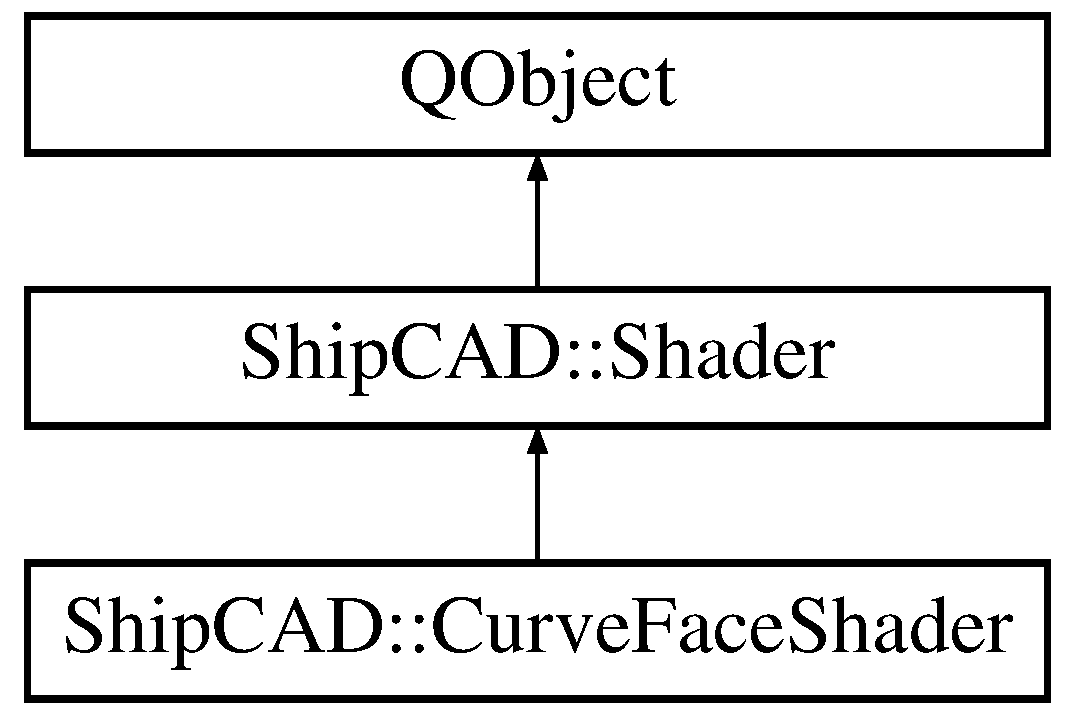
\includegraphics[height=3.000000cm]{classShipCAD_1_1CurveFaceShader}
\end{center}
\end{figure}
\subsection*{Public Member Functions}
\begin{DoxyCompactItemize}
\item 
\hyperlink{classShipCAD_1_1CurveFaceShader_acad5b622793dabf42d6be2a84bdc38dd}{Curve\+Face\+Shader} (\hyperlink{classShipCAD_1_1Viewport}{Viewport} $\ast$vp)
\item 
virtual \hyperlink{classShipCAD_1_1CurveFaceShader_af99773914de0758627d57aae99b5d44b}{$\sim$\+Curve\+Face\+Shader} ()
\item 
void \hyperlink{classShipCAD_1_1CurveFaceShader_aff6cca39c6e9c17c7dee2040724c5946}{set\+Matrices} (const Q\+Matrix4x4 \&proj, const Q\+Matrix4x4 \&view, const Q\+Matrix4x4 \&world)
\item 
virtual void \hyperlink{classShipCAD_1_1CurveFaceShader_ab817219da96b3dc744b19ee93f466a1f}{render\+Mesh} (Q\+Vector$<$ Q\+Vector3D $>$ \&vertices, Q\+Vector$<$ Q\+Vector3D $>$ \&colors, Q\+Vector$<$ Q\+Vector3D $>$ \&normals)
\end{DoxyCompactItemize}
\subsection*{Additional Inherited Members}


\subsection{Detailed Description}


Definition at line 152 of file shader.\+h.



\subsection{Constructor \& Destructor Documentation}
\index{Ship\+C\+A\+D\+::\+Curve\+Face\+Shader@{Ship\+C\+A\+D\+::\+Curve\+Face\+Shader}!Curve\+Face\+Shader@{Curve\+Face\+Shader}}
\index{Curve\+Face\+Shader@{Curve\+Face\+Shader}!Ship\+C\+A\+D\+::\+Curve\+Face\+Shader@{Ship\+C\+A\+D\+::\+Curve\+Face\+Shader}}
\subsubsection[{\texorpdfstring{Curve\+Face\+Shader(\+Viewport $\ast$vp)}{CurveFaceShader(Viewport *vp)}}]{\setlength{\rightskip}{0pt plus 5cm}Curve\+Face\+Shader\+::\+Curve\+Face\+Shader (
\begin{DoxyParamCaption}
\item[{{\bf Viewport} $\ast$}]{vp}
\end{DoxyParamCaption}
)\hspace{0.3cm}{\ttfamily [explicit]}}\hypertarget{classShipCAD_1_1CurveFaceShader_acad5b622793dabf42d6be2a84bdc38dd}{}\label{classShipCAD_1_1CurveFaceShader_acad5b622793dabf42d6be2a84bdc38dd}


Definition at line 366 of file shader.\+cpp.

\index{Ship\+C\+A\+D\+::\+Curve\+Face\+Shader@{Ship\+C\+A\+D\+::\+Curve\+Face\+Shader}!````~Curve\+Face\+Shader@{$\sim$\+Curve\+Face\+Shader}}
\index{````~Curve\+Face\+Shader@{$\sim$\+Curve\+Face\+Shader}!Ship\+C\+A\+D\+::\+Curve\+Face\+Shader@{Ship\+C\+A\+D\+::\+Curve\+Face\+Shader}}
\subsubsection[{\texorpdfstring{$\sim$\+Curve\+Face\+Shader()}{~CurveFaceShader()}}]{\setlength{\rightskip}{0pt plus 5cm}virtual Ship\+C\+A\+D\+::\+Curve\+Face\+Shader\+::$\sim$\+Curve\+Face\+Shader (
\begin{DoxyParamCaption}
{}
\end{DoxyParamCaption}
)\hspace{0.3cm}{\ttfamily [inline]}, {\ttfamily [virtual]}}\hypertarget{classShipCAD_1_1CurveFaceShader_af99773914de0758627d57aae99b5d44b}{}\label{classShipCAD_1_1CurveFaceShader_af99773914de0758627d57aae99b5d44b}


Definition at line 159 of file shader.\+h.



\subsection{Member Function Documentation}
\index{Ship\+C\+A\+D\+::\+Curve\+Face\+Shader@{Ship\+C\+A\+D\+::\+Curve\+Face\+Shader}!render\+Mesh@{render\+Mesh}}
\index{render\+Mesh@{render\+Mesh}!Ship\+C\+A\+D\+::\+Curve\+Face\+Shader@{Ship\+C\+A\+D\+::\+Curve\+Face\+Shader}}
\subsubsection[{\texorpdfstring{render\+Mesh(\+Q\+Vector$<$ Q\+Vector3\+D $>$ \&vertices, Q\+Vector$<$ Q\+Vector3\+D $>$ \&colors, Q\+Vector$<$ Q\+Vector3\+D $>$ \&normals)}{renderMesh(QVector< QVector3D > &vertices, QVector< QVector3D > &colors, QVector< QVector3D > &normals)}}]{\setlength{\rightskip}{0pt plus 5cm}void Curve\+Face\+Shader\+::render\+Mesh (
\begin{DoxyParamCaption}
\item[{Q\+Vector$<$ Q\+Vector3D $>$ \&}]{vertices, }
\item[{Q\+Vector$<$ Q\+Vector3D $>$ \&}]{colors, }
\item[{Q\+Vector$<$ Q\+Vector3D $>$ \&}]{normals}
\end{DoxyParamCaption}
)\hspace{0.3cm}{\ttfamily [virtual]}}\hypertarget{classShipCAD_1_1CurveFaceShader_ab817219da96b3dc744b19ee93f466a1f}{}\label{classShipCAD_1_1CurveFaceShader_ab817219da96b3dc744b19ee93f466a1f}


Definition at line 390 of file shader.\+cpp.

\index{Ship\+C\+A\+D\+::\+Curve\+Face\+Shader@{Ship\+C\+A\+D\+::\+Curve\+Face\+Shader}!set\+Matrices@{set\+Matrices}}
\index{set\+Matrices@{set\+Matrices}!Ship\+C\+A\+D\+::\+Curve\+Face\+Shader@{Ship\+C\+A\+D\+::\+Curve\+Face\+Shader}}
\subsubsection[{\texorpdfstring{set\+Matrices(const Q\+Matrix4x4 \&proj, const Q\+Matrix4x4 \&view, const Q\+Matrix4x4 \&world)}{setMatrices(const QMatrix4x4 &proj, const QMatrix4x4 &view, const QMatrix4x4 &world)}}]{\setlength{\rightskip}{0pt plus 5cm}void Curve\+Face\+Shader\+::set\+Matrices (
\begin{DoxyParamCaption}
\item[{const Q\+Matrix4x4 \&}]{proj, }
\item[{const Q\+Matrix4x4 \&}]{view, }
\item[{const Q\+Matrix4x4 \&}]{world}
\end{DoxyParamCaption}
)}\hypertarget{classShipCAD_1_1CurveFaceShader_aff6cca39c6e9c17c7dee2040724c5946}{}\label{classShipCAD_1_1CurveFaceShader_aff6cca39c6e9c17c7dee2040724c5946}


Definition at line 381 of file shader.\+cpp.



The documentation for this class was generated from the following files\+:\begin{DoxyCompactItemize}
\item 
Ship\+C\+A\+Dlib/\hyperlink{shader_8h}{shader.\+h}\item 
Ship\+C\+A\+Dlib/\hyperlink{shader_8cpp}{shader.\+cpp}\end{DoxyCompactItemize}

\hypertarget{classShipCAD_1_1DeleteElementsCollection}{}\section{Ship\+C\+AD\+:\+:Delete\+Elements\+Collection Class Reference}
\label{classShipCAD_1_1DeleteElementsCollection}\index{Ship\+C\+A\+D\+::\+Delete\+Elements\+Collection@{Ship\+C\+A\+D\+::\+Delete\+Elements\+Collection}}


{\ttfamily \#include $<$subdivsurface.\+h$>$}

\subsection*{Public Member Functions}
\begin{DoxyCompactItemize}
\item 
\hyperlink{classShipCAD_1_1DeleteElementsCollection_af90e27d3cab0018d689c1dfbbceeb8b9}{Delete\+Elements\+Collection} ()
\item 
void \hyperlink{classShipCAD_1_1DeleteElementsCollection_a42e99c010dff8fa9da3bccc6747b3b00}{clear} ()
\item 
bool \hyperlink{classShipCAD_1_1DeleteElementsCollection_a933c0b0679bf4b4d0017e7bb791001ef}{is\+Suppressed} () const 
\item 
void \hyperlink{classShipCAD_1_1DeleteElementsCollection_a6e6bd4397f891b9db53647ccc8444d0b}{suppress\+Delete} (bool on)
\end{DoxyCompactItemize}
\subsection*{Public Attributes}
\begin{DoxyCompactItemize}
\item 
std\+::set$<$ \hyperlink{classShipCAD_1_1SubdivisionControlPoint}{Subdivision\+Control\+Point} $\ast$ $>$ \hyperlink{classShipCAD_1_1DeleteElementsCollection_a7e5748f6463683b23a8b762ceadeb49a}{points}
\item 
std\+::set$<$ \hyperlink{classShipCAD_1_1SubdivisionControlEdge}{Subdivision\+Control\+Edge} $\ast$ $>$ \hyperlink{classShipCAD_1_1DeleteElementsCollection_a43038e1787626cde31dcb023366d886d}{edges}
\item 
std\+::set$<$ \hyperlink{classShipCAD_1_1SubdivisionControlFace}{Subdivision\+Control\+Face} $\ast$ $>$ \hyperlink{classShipCAD_1_1DeleteElementsCollection_ad032ba30c3ca251e710d0cb02abeb3d2}{faces}
\item 
std\+::set$<$ \hyperlink{classShipCAD_1_1SubdivisionControlCurve}{Subdivision\+Control\+Curve} $\ast$ $>$ \hyperlink{classShipCAD_1_1DeleteElementsCollection_a9d5c12e9ab17876c05a598419f79f5a4}{curves}
\item 
std\+::set$<$ \hyperlink{classShipCAD_1_1Spline}{Spline} $\ast$ $>$ \hyperlink{classShipCAD_1_1DeleteElementsCollection_a80150f5eea2654362d89f14105212c1c}{splines}
\end{DoxyCompactItemize}


\subsection{Detailed Description}


Definition at line 71 of file subdivsurface.\+h.



\subsection{Constructor \& Destructor Documentation}
\index{Ship\+C\+A\+D\+::\+Delete\+Elements\+Collection@{Ship\+C\+A\+D\+::\+Delete\+Elements\+Collection}!Delete\+Elements\+Collection@{Delete\+Elements\+Collection}}
\index{Delete\+Elements\+Collection@{Delete\+Elements\+Collection}!Ship\+C\+A\+D\+::\+Delete\+Elements\+Collection@{Ship\+C\+A\+D\+::\+Delete\+Elements\+Collection}}
\subsubsection[{\texorpdfstring{Delete\+Elements\+Collection()}{DeleteElementsCollection()}}]{\setlength{\rightskip}{0pt plus 5cm}Delete\+Elements\+Collection\+::\+Delete\+Elements\+Collection (
\begin{DoxyParamCaption}
{}
\end{DoxyParamCaption}
)\hspace{0.3cm}{\ttfamily [explicit]}}\hypertarget{classShipCAD_1_1DeleteElementsCollection_af90e27d3cab0018d689c1dfbbceeb8b9}{}\label{classShipCAD_1_1DeleteElementsCollection_af90e27d3cab0018d689c1dfbbceeb8b9}


Definition at line 61 of file subdivsurface.\+cpp.



\subsection{Member Function Documentation}
\index{Ship\+C\+A\+D\+::\+Delete\+Elements\+Collection@{Ship\+C\+A\+D\+::\+Delete\+Elements\+Collection}!clear@{clear}}
\index{clear@{clear}!Ship\+C\+A\+D\+::\+Delete\+Elements\+Collection@{Ship\+C\+A\+D\+::\+Delete\+Elements\+Collection}}
\subsubsection[{\texorpdfstring{clear()}{clear()}}]{\setlength{\rightskip}{0pt plus 5cm}void Delete\+Elements\+Collection\+::clear (
\begin{DoxyParamCaption}
{}
\end{DoxyParamCaption}
)}\hypertarget{classShipCAD_1_1DeleteElementsCollection_a42e99c010dff8fa9da3bccc6747b3b00}{}\label{classShipCAD_1_1DeleteElementsCollection_a42e99c010dff8fa9da3bccc6747b3b00}


Definition at line 67 of file subdivsurface.\+cpp.

\index{Ship\+C\+A\+D\+::\+Delete\+Elements\+Collection@{Ship\+C\+A\+D\+::\+Delete\+Elements\+Collection}!is\+Suppressed@{is\+Suppressed}}
\index{is\+Suppressed@{is\+Suppressed}!Ship\+C\+A\+D\+::\+Delete\+Elements\+Collection@{Ship\+C\+A\+D\+::\+Delete\+Elements\+Collection}}
\subsubsection[{\texorpdfstring{is\+Suppressed() const }{isSuppressed() const }}]{\setlength{\rightskip}{0pt plus 5cm}bool Ship\+C\+A\+D\+::\+Delete\+Elements\+Collection\+::is\+Suppressed (
\begin{DoxyParamCaption}
{}
\end{DoxyParamCaption}
) const\hspace{0.3cm}{\ttfamily [inline]}}\hypertarget{classShipCAD_1_1DeleteElementsCollection_a933c0b0679bf4b4d0017e7bb791001ef}{}\label{classShipCAD_1_1DeleteElementsCollection_a933c0b0679bf4b4d0017e7bb791001ef}


Definition at line 83 of file subdivsurface.\+h.

\index{Ship\+C\+A\+D\+::\+Delete\+Elements\+Collection@{Ship\+C\+A\+D\+::\+Delete\+Elements\+Collection}!suppress\+Delete@{suppress\+Delete}}
\index{suppress\+Delete@{suppress\+Delete}!Ship\+C\+A\+D\+::\+Delete\+Elements\+Collection@{Ship\+C\+A\+D\+::\+Delete\+Elements\+Collection}}
\subsubsection[{\texorpdfstring{suppress\+Delete(bool on)}{suppressDelete(bool on)}}]{\setlength{\rightskip}{0pt plus 5cm}void Ship\+C\+A\+D\+::\+Delete\+Elements\+Collection\+::suppress\+Delete (
\begin{DoxyParamCaption}
\item[{bool}]{on}
\end{DoxyParamCaption}
)\hspace{0.3cm}{\ttfamily [inline]}}\hypertarget{classShipCAD_1_1DeleteElementsCollection_a6e6bd4397f891b9db53647ccc8444d0b}{}\label{classShipCAD_1_1DeleteElementsCollection_a6e6bd4397f891b9db53647ccc8444d0b}


Definition at line 85 of file subdivsurface.\+h.



\subsection{Member Data Documentation}
\index{Ship\+C\+A\+D\+::\+Delete\+Elements\+Collection@{Ship\+C\+A\+D\+::\+Delete\+Elements\+Collection}!curves@{curves}}
\index{curves@{curves}!Ship\+C\+A\+D\+::\+Delete\+Elements\+Collection@{Ship\+C\+A\+D\+::\+Delete\+Elements\+Collection}}
\subsubsection[{\texorpdfstring{curves}{curves}}]{\setlength{\rightskip}{0pt plus 5cm}std\+::set$<${\bf Subdivision\+Control\+Curve}$\ast$$>$ Ship\+C\+A\+D\+::\+Delete\+Elements\+Collection\+::curves}\hypertarget{classShipCAD_1_1DeleteElementsCollection_a9d5c12e9ab17876c05a598419f79f5a4}{}\label{classShipCAD_1_1DeleteElementsCollection_a9d5c12e9ab17876c05a598419f79f5a4}


Definition at line 77 of file subdivsurface.\+h.

\index{Ship\+C\+A\+D\+::\+Delete\+Elements\+Collection@{Ship\+C\+A\+D\+::\+Delete\+Elements\+Collection}!edges@{edges}}
\index{edges@{edges}!Ship\+C\+A\+D\+::\+Delete\+Elements\+Collection@{Ship\+C\+A\+D\+::\+Delete\+Elements\+Collection}}
\subsubsection[{\texorpdfstring{edges}{edges}}]{\setlength{\rightskip}{0pt plus 5cm}std\+::set$<${\bf Subdivision\+Control\+Edge}$\ast$$>$ Ship\+C\+A\+D\+::\+Delete\+Elements\+Collection\+::edges}\hypertarget{classShipCAD_1_1DeleteElementsCollection_a43038e1787626cde31dcb023366d886d}{}\label{classShipCAD_1_1DeleteElementsCollection_a43038e1787626cde31dcb023366d886d}


Definition at line 75 of file subdivsurface.\+h.

\index{Ship\+C\+A\+D\+::\+Delete\+Elements\+Collection@{Ship\+C\+A\+D\+::\+Delete\+Elements\+Collection}!faces@{faces}}
\index{faces@{faces}!Ship\+C\+A\+D\+::\+Delete\+Elements\+Collection@{Ship\+C\+A\+D\+::\+Delete\+Elements\+Collection}}
\subsubsection[{\texorpdfstring{faces}{faces}}]{\setlength{\rightskip}{0pt plus 5cm}std\+::set$<${\bf Subdivision\+Control\+Face}$\ast$$>$ Ship\+C\+A\+D\+::\+Delete\+Elements\+Collection\+::faces}\hypertarget{classShipCAD_1_1DeleteElementsCollection_ad032ba30c3ca251e710d0cb02abeb3d2}{}\label{classShipCAD_1_1DeleteElementsCollection_ad032ba30c3ca251e710d0cb02abeb3d2}


Definition at line 76 of file subdivsurface.\+h.

\index{Ship\+C\+A\+D\+::\+Delete\+Elements\+Collection@{Ship\+C\+A\+D\+::\+Delete\+Elements\+Collection}!points@{points}}
\index{points@{points}!Ship\+C\+A\+D\+::\+Delete\+Elements\+Collection@{Ship\+C\+A\+D\+::\+Delete\+Elements\+Collection}}
\subsubsection[{\texorpdfstring{points}{points}}]{\setlength{\rightskip}{0pt plus 5cm}std\+::set$<${\bf Subdivision\+Control\+Point}$\ast$$>$ Ship\+C\+A\+D\+::\+Delete\+Elements\+Collection\+::points}\hypertarget{classShipCAD_1_1DeleteElementsCollection_a7e5748f6463683b23a8b762ceadeb49a}{}\label{classShipCAD_1_1DeleteElementsCollection_a7e5748f6463683b23a8b762ceadeb49a}


Definition at line 74 of file subdivsurface.\+h.

\index{Ship\+C\+A\+D\+::\+Delete\+Elements\+Collection@{Ship\+C\+A\+D\+::\+Delete\+Elements\+Collection}!splines@{splines}}
\index{splines@{splines}!Ship\+C\+A\+D\+::\+Delete\+Elements\+Collection@{Ship\+C\+A\+D\+::\+Delete\+Elements\+Collection}}
\subsubsection[{\texorpdfstring{splines}{splines}}]{\setlength{\rightskip}{0pt plus 5cm}std\+::set$<${\bf Spline}$\ast$$>$ Ship\+C\+A\+D\+::\+Delete\+Elements\+Collection\+::splines}\hypertarget{classShipCAD_1_1DeleteElementsCollection_a80150f5eea2654362d89f14105212c1c}{}\label{classShipCAD_1_1DeleteElementsCollection_a80150f5eea2654362d89f14105212c1c}


Definition at line 78 of file subdivsurface.\+h.



The documentation for this class was generated from the following files\+:\begin{DoxyCompactItemize}
\item 
Ship\+C\+A\+Dlib/\hyperlink{subdivsurface_8h}{subdivsurface.\+h}\item 
Ship\+C\+A\+Dlib/\hyperlink{subdivsurface_8cpp}{subdivsurface.\+cpp}\end{DoxyCompactItemize}

\hypertarget{structShipCAD_1_1DelftSeriesResistance}{}\section{Ship\+C\+AD\+:\+:Delft\+Series\+Resistance Struct Reference}
\label{structShipCAD_1_1DelftSeriesResistance}\index{Ship\+C\+A\+D\+::\+Delft\+Series\+Resistance@{Ship\+C\+A\+D\+::\+Delft\+Series\+Resistance}}


{\ttfamily \#include $<$resistance.\+h$>$}

\subsection*{Public Attributes}
\begin{DoxyCompactItemize}
\item 
float \hyperlink{structShipCAD_1_1DelftSeriesResistance_a040e0d678c7dbc24c29b7da618b4094d}{start\+\_\+speed}
\item 
float \hyperlink{structShipCAD_1_1DelftSeriesResistance_abd1672b905c07093735775ff455e5a98}{end\+\_\+speed}
\item 
float \hyperlink{structShipCAD_1_1DelftSeriesResistance_a0e3ee6d984afd4ddf1cf483261904574}{step\+\_\+speed}
\item 
float \hyperlink{structShipCAD_1_1DelftSeriesResistance_a160c7b99be523bcda5301231806af6b3}{bwl}
\item 
float \hyperlink{structShipCAD_1_1DelftSeriesResistance_ae489114ad6f1d03758420f77b58de519}{cp}
\item 
float \hyperlink{structShipCAD_1_1DelftSeriesResistance_a1c98fdc7b3c1b28f6f8029af2e009992}{displacement}
\item 
float \hyperlink{structShipCAD_1_1DelftSeriesResistance_a208e360c5ca0d029f9f433a7bc2cade2}{draft}
\item 
float \hyperlink{structShipCAD_1_1DelftSeriesResistance_a4db81049e448c381019f97dc630d51af}{draft\+\_\+total}
\item 
float \hyperlink{structShipCAD_1_1DelftSeriesResistance_a986244b5c6944f01dbdae5d54b895c84}{keel\+\_\+chord\+\_\+length}
\item 
float \hyperlink{structShipCAD_1_1DelftSeriesResistance_ab1bf49519c2ed054b7699898d7f5aead}{keel\+\_\+area}
\item 
float \hyperlink{structShipCAD_1_1DelftSeriesResistance_aca93b2c11316e29b2f98a3bdcdf65bc5}{lcb}
\item 
float \hyperlink{structShipCAD_1_1DelftSeriesResistance_a7232b8ea3003087a4772a650319ec8f2}{lwl}
\item 
float \hyperlink{structShipCAD_1_1DelftSeriesResistance_a5a348a92e0ba99368c50f72c81a9b0ff}{rudder\+\_\+chord\+\_\+length}
\item 
float \hyperlink{structShipCAD_1_1DelftSeriesResistance_a9737974d43a292c58a2e24f7c78c1ffb}{rudder\+\_\+area}
\item 
float \hyperlink{structShipCAD_1_1DelftSeriesResistance_a08ff900d51b56d7e1726cb4b5a6ffa9b}{viscosity}
\item 
float \hyperlink{structShipCAD_1_1DelftSeriesResistance_a7ee0a7e2d05634beb7fb9951d80c7557}{wetted\+\_\+surface}
\item 
float \hyperlink{structShipCAD_1_1DelftSeriesResistance_af51e72b70af1ce87cf7ac641df93c541}{wl\+\_\+area}
\item 
bool \hyperlink{structShipCAD_1_1DelftSeriesResistance_a0507b03a9329185d961cd97739237d91}{estimate\+\_\+wet\+\_\+surf}
\item 
bool \hyperlink{structShipCAD_1_1DelftSeriesResistance_a8276aa04952e727f1a310f10ceb72414}{extract}
\item 
quint8 \hyperlink{structShipCAD_1_1DelftSeriesResistance_acd08ff15cfab748bf4f54aa65b927950}{padding} \mbox{[}2\mbox{]}
\end{DoxyCompactItemize}


\subsection{Detailed Description}


Definition at line 38 of file resistance.\+h.



\subsection{Member Data Documentation}
\index{Ship\+C\+A\+D\+::\+Delft\+Series\+Resistance@{Ship\+C\+A\+D\+::\+Delft\+Series\+Resistance}!bwl@{bwl}}
\index{bwl@{bwl}!Ship\+C\+A\+D\+::\+Delft\+Series\+Resistance@{Ship\+C\+A\+D\+::\+Delft\+Series\+Resistance}}
\subsubsection[{\texorpdfstring{bwl}{bwl}}]{\setlength{\rightskip}{0pt plus 5cm}float Ship\+C\+A\+D\+::\+Delft\+Series\+Resistance\+::bwl}\hypertarget{structShipCAD_1_1DelftSeriesResistance_a160c7b99be523bcda5301231806af6b3}{}\label{structShipCAD_1_1DelftSeriesResistance_a160c7b99be523bcda5301231806af6b3}


Definition at line 43 of file resistance.\+h.

\index{Ship\+C\+A\+D\+::\+Delft\+Series\+Resistance@{Ship\+C\+A\+D\+::\+Delft\+Series\+Resistance}!cp@{cp}}
\index{cp@{cp}!Ship\+C\+A\+D\+::\+Delft\+Series\+Resistance@{Ship\+C\+A\+D\+::\+Delft\+Series\+Resistance}}
\subsubsection[{\texorpdfstring{cp}{cp}}]{\setlength{\rightskip}{0pt plus 5cm}float Ship\+C\+A\+D\+::\+Delft\+Series\+Resistance\+::cp}\hypertarget{structShipCAD_1_1DelftSeriesResistance_ae489114ad6f1d03758420f77b58de519}{}\label{structShipCAD_1_1DelftSeriesResistance_ae489114ad6f1d03758420f77b58de519}


Definition at line 44 of file resistance.\+h.

\index{Ship\+C\+A\+D\+::\+Delft\+Series\+Resistance@{Ship\+C\+A\+D\+::\+Delft\+Series\+Resistance}!displacement@{displacement}}
\index{displacement@{displacement}!Ship\+C\+A\+D\+::\+Delft\+Series\+Resistance@{Ship\+C\+A\+D\+::\+Delft\+Series\+Resistance}}
\subsubsection[{\texorpdfstring{displacement}{displacement}}]{\setlength{\rightskip}{0pt plus 5cm}float Ship\+C\+A\+D\+::\+Delft\+Series\+Resistance\+::displacement}\hypertarget{structShipCAD_1_1DelftSeriesResistance_a1c98fdc7b3c1b28f6f8029af2e009992}{}\label{structShipCAD_1_1DelftSeriesResistance_a1c98fdc7b3c1b28f6f8029af2e009992}


Definition at line 45 of file resistance.\+h.

\index{Ship\+C\+A\+D\+::\+Delft\+Series\+Resistance@{Ship\+C\+A\+D\+::\+Delft\+Series\+Resistance}!draft@{draft}}
\index{draft@{draft}!Ship\+C\+A\+D\+::\+Delft\+Series\+Resistance@{Ship\+C\+A\+D\+::\+Delft\+Series\+Resistance}}
\subsubsection[{\texorpdfstring{draft}{draft}}]{\setlength{\rightskip}{0pt plus 5cm}float Ship\+C\+A\+D\+::\+Delft\+Series\+Resistance\+::draft}\hypertarget{structShipCAD_1_1DelftSeriesResistance_a208e360c5ca0d029f9f433a7bc2cade2}{}\label{structShipCAD_1_1DelftSeriesResistance_a208e360c5ca0d029f9f433a7bc2cade2}


Definition at line 46 of file resistance.\+h.

\index{Ship\+C\+A\+D\+::\+Delft\+Series\+Resistance@{Ship\+C\+A\+D\+::\+Delft\+Series\+Resistance}!draft\+\_\+total@{draft\+\_\+total}}
\index{draft\+\_\+total@{draft\+\_\+total}!Ship\+C\+A\+D\+::\+Delft\+Series\+Resistance@{Ship\+C\+A\+D\+::\+Delft\+Series\+Resistance}}
\subsubsection[{\texorpdfstring{draft\+\_\+total}{draft_total}}]{\setlength{\rightskip}{0pt plus 5cm}float Ship\+C\+A\+D\+::\+Delft\+Series\+Resistance\+::draft\+\_\+total}\hypertarget{structShipCAD_1_1DelftSeriesResistance_a4db81049e448c381019f97dc630d51af}{}\label{structShipCAD_1_1DelftSeriesResistance_a4db81049e448c381019f97dc630d51af}


Definition at line 47 of file resistance.\+h.

\index{Ship\+C\+A\+D\+::\+Delft\+Series\+Resistance@{Ship\+C\+A\+D\+::\+Delft\+Series\+Resistance}!end\+\_\+speed@{end\+\_\+speed}}
\index{end\+\_\+speed@{end\+\_\+speed}!Ship\+C\+A\+D\+::\+Delft\+Series\+Resistance@{Ship\+C\+A\+D\+::\+Delft\+Series\+Resistance}}
\subsubsection[{\texorpdfstring{end\+\_\+speed}{end_speed}}]{\setlength{\rightskip}{0pt plus 5cm}float Ship\+C\+A\+D\+::\+Delft\+Series\+Resistance\+::end\+\_\+speed}\hypertarget{structShipCAD_1_1DelftSeriesResistance_abd1672b905c07093735775ff455e5a98}{}\label{structShipCAD_1_1DelftSeriesResistance_abd1672b905c07093735775ff455e5a98}


Definition at line 41 of file resistance.\+h.

\index{Ship\+C\+A\+D\+::\+Delft\+Series\+Resistance@{Ship\+C\+A\+D\+::\+Delft\+Series\+Resistance}!estimate\+\_\+wet\+\_\+surf@{estimate\+\_\+wet\+\_\+surf}}
\index{estimate\+\_\+wet\+\_\+surf@{estimate\+\_\+wet\+\_\+surf}!Ship\+C\+A\+D\+::\+Delft\+Series\+Resistance@{Ship\+C\+A\+D\+::\+Delft\+Series\+Resistance}}
\subsubsection[{\texorpdfstring{estimate\+\_\+wet\+\_\+surf}{estimate_wet_surf}}]{\setlength{\rightskip}{0pt plus 5cm}bool Ship\+C\+A\+D\+::\+Delft\+Series\+Resistance\+::estimate\+\_\+wet\+\_\+surf}\hypertarget{structShipCAD_1_1DelftSeriesResistance_a0507b03a9329185d961cd97739237d91}{}\label{structShipCAD_1_1DelftSeriesResistance_a0507b03a9329185d961cd97739237d91}


Definition at line 57 of file resistance.\+h.

\index{Ship\+C\+A\+D\+::\+Delft\+Series\+Resistance@{Ship\+C\+A\+D\+::\+Delft\+Series\+Resistance}!extract@{extract}}
\index{extract@{extract}!Ship\+C\+A\+D\+::\+Delft\+Series\+Resistance@{Ship\+C\+A\+D\+::\+Delft\+Series\+Resistance}}
\subsubsection[{\texorpdfstring{extract}{extract}}]{\setlength{\rightskip}{0pt plus 5cm}bool Ship\+C\+A\+D\+::\+Delft\+Series\+Resistance\+::extract}\hypertarget{structShipCAD_1_1DelftSeriesResistance_a8276aa04952e727f1a310f10ceb72414}{}\label{structShipCAD_1_1DelftSeriesResistance_a8276aa04952e727f1a310f10ceb72414}


Definition at line 58 of file resistance.\+h.

\index{Ship\+C\+A\+D\+::\+Delft\+Series\+Resistance@{Ship\+C\+A\+D\+::\+Delft\+Series\+Resistance}!keel\+\_\+area@{keel\+\_\+area}}
\index{keel\+\_\+area@{keel\+\_\+area}!Ship\+C\+A\+D\+::\+Delft\+Series\+Resistance@{Ship\+C\+A\+D\+::\+Delft\+Series\+Resistance}}
\subsubsection[{\texorpdfstring{keel\+\_\+area}{keel_area}}]{\setlength{\rightskip}{0pt plus 5cm}float Ship\+C\+A\+D\+::\+Delft\+Series\+Resistance\+::keel\+\_\+area}\hypertarget{structShipCAD_1_1DelftSeriesResistance_ab1bf49519c2ed054b7699898d7f5aead}{}\label{structShipCAD_1_1DelftSeriesResistance_ab1bf49519c2ed054b7699898d7f5aead}


Definition at line 49 of file resistance.\+h.

\index{Ship\+C\+A\+D\+::\+Delft\+Series\+Resistance@{Ship\+C\+A\+D\+::\+Delft\+Series\+Resistance}!keel\+\_\+chord\+\_\+length@{keel\+\_\+chord\+\_\+length}}
\index{keel\+\_\+chord\+\_\+length@{keel\+\_\+chord\+\_\+length}!Ship\+C\+A\+D\+::\+Delft\+Series\+Resistance@{Ship\+C\+A\+D\+::\+Delft\+Series\+Resistance}}
\subsubsection[{\texorpdfstring{keel\+\_\+chord\+\_\+length}{keel_chord_length}}]{\setlength{\rightskip}{0pt plus 5cm}float Ship\+C\+A\+D\+::\+Delft\+Series\+Resistance\+::keel\+\_\+chord\+\_\+length}\hypertarget{structShipCAD_1_1DelftSeriesResistance_a986244b5c6944f01dbdae5d54b895c84}{}\label{structShipCAD_1_1DelftSeriesResistance_a986244b5c6944f01dbdae5d54b895c84}


Definition at line 48 of file resistance.\+h.

\index{Ship\+C\+A\+D\+::\+Delft\+Series\+Resistance@{Ship\+C\+A\+D\+::\+Delft\+Series\+Resistance}!lcb@{lcb}}
\index{lcb@{lcb}!Ship\+C\+A\+D\+::\+Delft\+Series\+Resistance@{Ship\+C\+A\+D\+::\+Delft\+Series\+Resistance}}
\subsubsection[{\texorpdfstring{lcb}{lcb}}]{\setlength{\rightskip}{0pt plus 5cm}float Ship\+C\+A\+D\+::\+Delft\+Series\+Resistance\+::lcb}\hypertarget{structShipCAD_1_1DelftSeriesResistance_aca93b2c11316e29b2f98a3bdcdf65bc5}{}\label{structShipCAD_1_1DelftSeriesResistance_aca93b2c11316e29b2f98a3bdcdf65bc5}


Definition at line 50 of file resistance.\+h.

\index{Ship\+C\+A\+D\+::\+Delft\+Series\+Resistance@{Ship\+C\+A\+D\+::\+Delft\+Series\+Resistance}!lwl@{lwl}}
\index{lwl@{lwl}!Ship\+C\+A\+D\+::\+Delft\+Series\+Resistance@{Ship\+C\+A\+D\+::\+Delft\+Series\+Resistance}}
\subsubsection[{\texorpdfstring{lwl}{lwl}}]{\setlength{\rightskip}{0pt plus 5cm}float Ship\+C\+A\+D\+::\+Delft\+Series\+Resistance\+::lwl}\hypertarget{structShipCAD_1_1DelftSeriesResistance_a7232b8ea3003087a4772a650319ec8f2}{}\label{structShipCAD_1_1DelftSeriesResistance_a7232b8ea3003087a4772a650319ec8f2}


Definition at line 51 of file resistance.\+h.

\index{Ship\+C\+A\+D\+::\+Delft\+Series\+Resistance@{Ship\+C\+A\+D\+::\+Delft\+Series\+Resistance}!padding@{padding}}
\index{padding@{padding}!Ship\+C\+A\+D\+::\+Delft\+Series\+Resistance@{Ship\+C\+A\+D\+::\+Delft\+Series\+Resistance}}
\subsubsection[{\texorpdfstring{padding}{padding}}]{\setlength{\rightskip}{0pt plus 5cm}quint8 Ship\+C\+A\+D\+::\+Delft\+Series\+Resistance\+::padding\mbox{[}2\mbox{]}}\hypertarget{structShipCAD_1_1DelftSeriesResistance_acd08ff15cfab748bf4f54aa65b927950}{}\label{structShipCAD_1_1DelftSeriesResistance_acd08ff15cfab748bf4f54aa65b927950}


Definition at line 63 of file resistance.\+h.

\index{Ship\+C\+A\+D\+::\+Delft\+Series\+Resistance@{Ship\+C\+A\+D\+::\+Delft\+Series\+Resistance}!rudder\+\_\+area@{rudder\+\_\+area}}
\index{rudder\+\_\+area@{rudder\+\_\+area}!Ship\+C\+A\+D\+::\+Delft\+Series\+Resistance@{Ship\+C\+A\+D\+::\+Delft\+Series\+Resistance}}
\subsubsection[{\texorpdfstring{rudder\+\_\+area}{rudder_area}}]{\setlength{\rightskip}{0pt plus 5cm}float Ship\+C\+A\+D\+::\+Delft\+Series\+Resistance\+::rudder\+\_\+area}\hypertarget{structShipCAD_1_1DelftSeriesResistance_a9737974d43a292c58a2e24f7c78c1ffb}{}\label{structShipCAD_1_1DelftSeriesResistance_a9737974d43a292c58a2e24f7c78c1ffb}


Definition at line 53 of file resistance.\+h.

\index{Ship\+C\+A\+D\+::\+Delft\+Series\+Resistance@{Ship\+C\+A\+D\+::\+Delft\+Series\+Resistance}!rudder\+\_\+chord\+\_\+length@{rudder\+\_\+chord\+\_\+length}}
\index{rudder\+\_\+chord\+\_\+length@{rudder\+\_\+chord\+\_\+length}!Ship\+C\+A\+D\+::\+Delft\+Series\+Resistance@{Ship\+C\+A\+D\+::\+Delft\+Series\+Resistance}}
\subsubsection[{\texorpdfstring{rudder\+\_\+chord\+\_\+length}{rudder_chord_length}}]{\setlength{\rightskip}{0pt plus 5cm}float Ship\+C\+A\+D\+::\+Delft\+Series\+Resistance\+::rudder\+\_\+chord\+\_\+length}\hypertarget{structShipCAD_1_1DelftSeriesResistance_a5a348a92e0ba99368c50f72c81a9b0ff}{}\label{structShipCAD_1_1DelftSeriesResistance_a5a348a92e0ba99368c50f72c81a9b0ff}


Definition at line 52 of file resistance.\+h.

\index{Ship\+C\+A\+D\+::\+Delft\+Series\+Resistance@{Ship\+C\+A\+D\+::\+Delft\+Series\+Resistance}!start\+\_\+speed@{start\+\_\+speed}}
\index{start\+\_\+speed@{start\+\_\+speed}!Ship\+C\+A\+D\+::\+Delft\+Series\+Resistance@{Ship\+C\+A\+D\+::\+Delft\+Series\+Resistance}}
\subsubsection[{\texorpdfstring{start\+\_\+speed}{start_speed}}]{\setlength{\rightskip}{0pt plus 5cm}float Ship\+C\+A\+D\+::\+Delft\+Series\+Resistance\+::start\+\_\+speed}\hypertarget{structShipCAD_1_1DelftSeriesResistance_a040e0d678c7dbc24c29b7da618b4094d}{}\label{structShipCAD_1_1DelftSeriesResistance_a040e0d678c7dbc24c29b7da618b4094d}


Definition at line 40 of file resistance.\+h.

\index{Ship\+C\+A\+D\+::\+Delft\+Series\+Resistance@{Ship\+C\+A\+D\+::\+Delft\+Series\+Resistance}!step\+\_\+speed@{step\+\_\+speed}}
\index{step\+\_\+speed@{step\+\_\+speed}!Ship\+C\+A\+D\+::\+Delft\+Series\+Resistance@{Ship\+C\+A\+D\+::\+Delft\+Series\+Resistance}}
\subsubsection[{\texorpdfstring{step\+\_\+speed}{step_speed}}]{\setlength{\rightskip}{0pt plus 5cm}float Ship\+C\+A\+D\+::\+Delft\+Series\+Resistance\+::step\+\_\+speed}\hypertarget{structShipCAD_1_1DelftSeriesResistance_a0e3ee6d984afd4ddf1cf483261904574}{}\label{structShipCAD_1_1DelftSeriesResistance_a0e3ee6d984afd4ddf1cf483261904574}


Definition at line 42 of file resistance.\+h.

\index{Ship\+C\+A\+D\+::\+Delft\+Series\+Resistance@{Ship\+C\+A\+D\+::\+Delft\+Series\+Resistance}!viscosity@{viscosity}}
\index{viscosity@{viscosity}!Ship\+C\+A\+D\+::\+Delft\+Series\+Resistance@{Ship\+C\+A\+D\+::\+Delft\+Series\+Resistance}}
\subsubsection[{\texorpdfstring{viscosity}{viscosity}}]{\setlength{\rightskip}{0pt plus 5cm}float Ship\+C\+A\+D\+::\+Delft\+Series\+Resistance\+::viscosity}\hypertarget{structShipCAD_1_1DelftSeriesResistance_a08ff900d51b56d7e1726cb4b5a6ffa9b}{}\label{structShipCAD_1_1DelftSeriesResistance_a08ff900d51b56d7e1726cb4b5a6ffa9b}


Definition at line 54 of file resistance.\+h.

\index{Ship\+C\+A\+D\+::\+Delft\+Series\+Resistance@{Ship\+C\+A\+D\+::\+Delft\+Series\+Resistance}!wetted\+\_\+surface@{wetted\+\_\+surface}}
\index{wetted\+\_\+surface@{wetted\+\_\+surface}!Ship\+C\+A\+D\+::\+Delft\+Series\+Resistance@{Ship\+C\+A\+D\+::\+Delft\+Series\+Resistance}}
\subsubsection[{\texorpdfstring{wetted\+\_\+surface}{wetted_surface}}]{\setlength{\rightskip}{0pt plus 5cm}float Ship\+C\+A\+D\+::\+Delft\+Series\+Resistance\+::wetted\+\_\+surface}\hypertarget{structShipCAD_1_1DelftSeriesResistance_a7ee0a7e2d05634beb7fb9951d80c7557}{}\label{structShipCAD_1_1DelftSeriesResistance_a7ee0a7e2d05634beb7fb9951d80c7557}


Definition at line 55 of file resistance.\+h.

\index{Ship\+C\+A\+D\+::\+Delft\+Series\+Resistance@{Ship\+C\+A\+D\+::\+Delft\+Series\+Resistance}!wl\+\_\+area@{wl\+\_\+area}}
\index{wl\+\_\+area@{wl\+\_\+area}!Ship\+C\+A\+D\+::\+Delft\+Series\+Resistance@{Ship\+C\+A\+D\+::\+Delft\+Series\+Resistance}}
\subsubsection[{\texorpdfstring{wl\+\_\+area}{wl_area}}]{\setlength{\rightskip}{0pt plus 5cm}float Ship\+C\+A\+D\+::\+Delft\+Series\+Resistance\+::wl\+\_\+area}\hypertarget{structShipCAD_1_1DelftSeriesResistance_af51e72b70af1ce87cf7ac641df93c541}{}\label{structShipCAD_1_1DelftSeriesResistance_af51e72b70af1ce87cf7ac641df93c541}


Definition at line 56 of file resistance.\+h.



The documentation for this struct was generated from the following file\+:\begin{DoxyCompactItemize}
\item 
Ship\+C\+A\+Dlib/\hyperlink{resistance_8h}{resistance.\+h}\end{DoxyCompactItemize}

\hypertarget{classShipCAD_1_1DevelopedPatch}{}\section{Ship\+C\+AD\+:\+:Developed\+Patch Class Reference}
\label{classShipCAD_1_1DevelopedPatch}\index{Ship\+C\+A\+D\+::\+Developed\+Patch@{Ship\+C\+A\+D\+::\+Developed\+Patch}}


base class for all non-\/surface drawable elements  




{\ttfamily \#include $<$developedpatch.\+h$>$}

Inheritance diagram for Ship\+C\+AD\+:\+:Developed\+Patch\+:\begin{figure}[H]
\begin{center}
\leavevmode
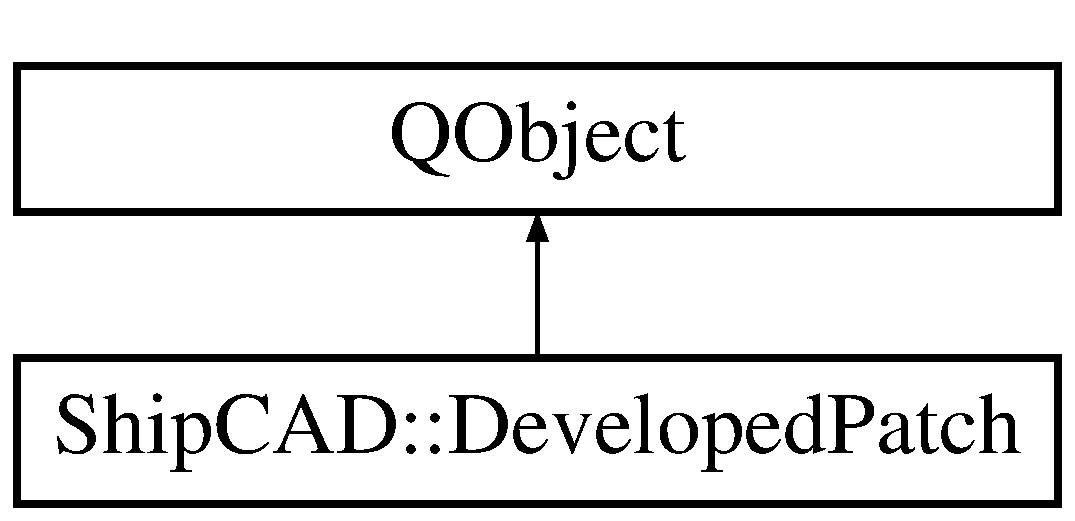
\includegraphics[height=2.000000cm]{classShipCAD_1_1DevelopedPatch}
\end{center}
\end{figure}
\subsection*{Public Member Functions}
\begin{DoxyCompactItemize}
\item 
\hyperlink{classShipCAD_1_1DevelopedPatch_ac204705b008b75aa3633a4025d14e518}{Developed\+Patch} (\hyperlink{classShipCAD_1_1SubdivisionLayer}{Subdivision\+Layer} $\ast$layer)
\item 
virtual \hyperlink{classShipCAD_1_1DevelopedPatch_a7e47417b03f9d91f891edb34441eb045}{$\sim$\+Developed\+Patch} ()
\item 
virtual void \hyperlink{classShipCAD_1_1DevelopedPatch_af3c4ba4cad20580cc8d5a4591b0bffd0}{clear} ()
\item 
virtual void \hyperlink{classShipCAD_1_1DevelopedPatch_a6d8a53701a952c0a6777e0b0c2ca6127}{extents} (Q\+Vector3D \&min, Q\+Vector3D \&max)
\item 
virtual void \hyperlink{classShipCAD_1_1DevelopedPatch_a7ba24420b1e8a1fb98acac3d38f8e37e}{draw} (\hyperlink{classShipCAD_1_1Viewport}{Viewport} \&vp, \hyperlink{classShipCAD_1_1LineShader}{Line\+Shader} $\ast$lineshader)
\item 
\hyperlink{classShipCAD_1_1SubdivisionLayer}{Subdivision\+Layer} $\ast$ \hyperlink{classShipCAD_1_1DevelopedPatch_a53dbb5c8582ded9fce56d81b3e79116d}{get\+Owner} ()
\item 
void \hyperlink{classShipCAD_1_1DevelopedPatch_a71eaddef96ee0edcefb7c15f07c65f7a}{intersect\+Plane} (\hyperlink{classShipCAD_1_1Plane}{Plane} \&plane, Q\+Color color)
\item 
Q\+Vector3D \hyperlink{classShipCAD_1_1DevelopedPatch_acd5b00b39301b249e3c019674dd67186}{convert\+To3D} (Q\+Vector2D p)
\item 
void \hyperlink{classShipCAD_1_1DevelopedPatch_a9ecc3812de9fd0999336c99a71774bbd}{save\+To\+D\+XF} (Q\+String\+List \&strings)
\item 
void \hyperlink{classShipCAD_1_1DevelopedPatch_a0528f08293c1ac8e53e3954c8c9e8585}{save\+To\+Text\+File} (Q\+String\+List \&strings)
\item 
void \hyperlink{classShipCAD_1_1DevelopedPatch_a55470422ecac9d544c811eddc8c3d1c1}{unroll} (std\+::vector$<$ \hyperlink{classShipCAD_1_1SubdivisionControlFace}{Subdivision\+Control\+Face} $\ast$ $>$ controlfaces)
\item 
double \hyperlink{classShipCAD_1_1DevelopedPatch_a4ddcf2a3bb1886d6210a89d5b524a2eb}{total\+Area\+Error} ()
\item 
double \hyperlink{classShipCAD_1_1DevelopedPatch_ae069aa101604151d0349805ffeb3902e}{max\+Area\+Error} ()
\item 
double \hyperlink{classShipCAD_1_1DevelopedPatch_a18ecaf8785655a33537ae155208b4c17}{max\+Error} ()
\item 
Q\+Vector2D \hyperlink{classShipCAD_1_1DevelopedPatch_a14dffbaa2c469eb825bb791c7c7cff42}{mid\+Point} ()
\item 
double \hyperlink{classShipCAD_1_1DevelopedPatch_a93c223c8eb2a39524cae8f71a863a15a}{min\+Error} ()
\item 
const Q\+String \& \hyperlink{classShipCAD_1_1DevelopedPatch_ab6918e553621440eef4efd9e4ae6fd2e}{name} ()
\item 
void \hyperlink{classShipCAD_1_1DevelopedPatch_a3ddb91773f49fa342f1fed811cd329f2}{set\+Name} (const Q\+String \&nm)
\item 
int \hyperlink{classShipCAD_1_1DevelopedPatch_a85be1d66371c43cedb1096bddf064e53}{number\+Of\+Iterations} ()
\item 
Q\+Vector3D \hyperlink{classShipCAD_1_1DevelopedPatch_a9cc5530b21f276b51279a2a46e261203}{get\+Point} (size\+\_\+t index)
\item 
Q\+Vector3D \hyperlink{classShipCAD_1_1DevelopedPatch_af7769b0032f7ca99b0790d1ae75d6d9f}{get\+Mirror\+Point} (size\+\_\+t index)
\item 
float \hyperlink{classShipCAD_1_1DevelopedPatch_a0a6aba001c536ddb4684d0c601ccc515}{rotation} ()
\item 
void \hyperlink{classShipCAD_1_1DevelopedPatch_ab91b09750cdae69f7f39b12980191f5e}{set\+Rotation} (float val)
\item 
Q\+Vector2D \hyperlink{classShipCAD_1_1DevelopedPatch_adce7adc7adf158ed0547a2dce708d8fe}{translation} ()
\item 
void \hyperlink{classShipCAD_1_1DevelopedPatch_a1c16b7311901ed24f90f5f99947438aa}{set\+Translation} (Q\+Vector2D val)
\item 
bool \hyperlink{classShipCAD_1_1DevelopedPatch_ae2a022f78ac1345f6ede335b32eadeb1}{is\+Mirror} ()
\item 
void \hyperlink{classShipCAD_1_1DevelopedPatch_a968873808a19604ecf04c9818f222fbb}{set\+Mirror} (bool set)
\item 
bool \hyperlink{classShipCAD_1_1DevelopedPatch_a58e6f298890172916af11e43ce9faedd}{mirror\+On\+Screen} ()
\item 
void \hyperlink{classShipCAD_1_1DevelopedPatch_a47e52017866102fdc68c2502dd56eb7f}{set\+Mirror\+On\+Screen} (bool set)
\item 
bool \hyperlink{classShipCAD_1_1DevelopedPatch_a3c9a16c7f2453d62b50e8ea40f9571e2}{is\+Shade\+Submerged} ()
\item 
void \hyperlink{classShipCAD_1_1DevelopedPatch_afd4cfdc14036055e13c1fcc2eaaaabda}{set\+Shade\+Submerged} (bool set)
\item 
bool \hyperlink{classShipCAD_1_1DevelopedPatch_a456f6b0ba40c8a6be86f81c45c9062c4}{show\+Bounding\+Box} ()
\item 
void \hyperlink{classShipCAD_1_1DevelopedPatch_a6adb505976cf4f01beba5774e2fa882b}{set\+Show\+Bounding\+Box} (bool set)
\item 
bool \hyperlink{classShipCAD_1_1DevelopedPatch_a3563a7434a34b0a46bb7ee0413851179}{show\+Buttocks} ()
\item 
void \hyperlink{classShipCAD_1_1DevelopedPatch_ab406b4350137fcf93cca71b2c05c44be}{set\+Show\+Buttocks} (bool set)
\item 
bool \hyperlink{classShipCAD_1_1DevelopedPatch_abb80ca80bb26c6d44995161517a34c2f}{show\+Diagonals} ()
\item 
void \hyperlink{classShipCAD_1_1DevelopedPatch_a9664cee0660a8e5d2ac41ff9056cc434}{set\+Show\+Diagonals} (bool set)
\item 
bool \hyperlink{classShipCAD_1_1DevelopedPatch_acab796afd80347da0b839511e0287fb1}{show\+Dimensions} ()
\item 
void \hyperlink{classShipCAD_1_1DevelopedPatch_abb6ef0e0db4819e5e70b6b1066f79736}{set\+Show\+Dimensions} (bool set)
\item 
bool \hyperlink{classShipCAD_1_1DevelopedPatch_aa6ab97dde9f6152f57b501b527cf9b34}{show\+Error\+Edges} ()
\item 
void \hyperlink{classShipCAD_1_1DevelopedPatch_a1e69c1d9755df1b77757bfd07b39f16a}{set\+Show\+Error\+Edges} (bool set)
\item 
bool \hyperlink{classShipCAD_1_1DevelopedPatch_adb0eefd6031d26224f17f7e8ce32b0a5}{show\+Interior\+Edges} ()
\item 
void \hyperlink{classShipCAD_1_1DevelopedPatch_ab580d449a859b81adfd2542ceea0464d}{set\+Show\+Interior\+Edges} (bool set)
\item 
bool \hyperlink{classShipCAD_1_1DevelopedPatch_a0ddb0069d07d2a27e709dc1f5c76275b}{show\+Part\+Name} ()
\item 
void \hyperlink{classShipCAD_1_1DevelopedPatch_a9ece9e74aa65a84117568b0f0c74ef0b}{set\+Show\+Part\+Name} (bool set)
\item 
bool \hyperlink{classShipCAD_1_1DevelopedPatch_a244492f9f03b465b7573fd7ee0556ad8}{show\+Solid} ()
\item 
void \hyperlink{classShipCAD_1_1DevelopedPatch_aba39dc6408881f90dc08c90779c7b1a6}{set\+Show\+Solid} (bool set)
\item 
bool \hyperlink{classShipCAD_1_1DevelopedPatch_a98e0c1b8c6302ce1beb475fb4590f483}{show\+Stations} ()
\item 
void \hyperlink{classShipCAD_1_1DevelopedPatch_a7780c1a8816517c8bccadc4a9fe64b29}{set\+Show\+Stations} (bool set)
\item 
bool \hyperlink{classShipCAD_1_1DevelopedPatch_adbab0c37bf68eff8e68c272051fa6a94}{show\+Waterlines} ()
\item 
void \hyperlink{classShipCAD_1_1DevelopedPatch_ac3daa557956f05c5ed4eb2da52706a85}{set\+Show\+Waterlines} (bool set)
\item 
void \hyperlink{classShipCAD_1_1DevelopedPatch_ae4f82982b3828b99f27c11ab20132516}{dump} (std\+::ostream \&os) const 
\end{DoxyCompactItemize}
\subsection*{Protected Member Functions}
\begin{DoxyCompactItemize}
\item 
void \hyperlink{classShipCAD_1_1DevelopedPatch_aba8c1bb34e8690b2192b3cc2c389bad9}{export\+Spline} (Q\+String\+List \&strings, \hyperlink{classShipCAD_1_1Spline}{Spline} $\ast$spline, const Q\+String \&layername)
\item 
\hyperlink{namespaceShipCAD_a22a4489ec7a6505c3c30fa7562175ca4}{Polygon\+Orientation} \hyperlink{classShipCAD_1_1DevelopedPatch_a3210c1289d04ec78d1a13217b5ea742a}{crossproduct} (const Q\+Vector2D \&p1, const Q\+Vector2D \&p2, const Q\+Vector2D \&p3)
\item 
Q\+Vector2D \hyperlink{classShipCAD_1_1DevelopedPatch_aaa57f091d14d72af632b838a1cfd39c0}{calculate\+Triangle} (double a, double b, double c, const Q\+Vector2D \&p1, const Q\+Vector2D \&p2)
\item 
Q\+Vector2D \hyperlink{classShipCAD_1_1DevelopedPatch_a3c4527d0a0fcafff2b506aabef67a43e}{calculate\+Triangle2} (double a, double b, double c, const Q\+Vector2D \&p1, const Q\+Vector2D \&p2)
\item 
void \hyperlink{classShipCAD_1_1DevelopedPatch_af5563e813910e11a78126223a6635faf}{unroll2D} (\hyperlink{classShipCAD_1_1SubdivisionFace}{Subdivision\+Face} $\ast$face, bool \&firstface, bool \&error, \hyperlink{namespaceShipCAD_a22a4489ec7a6505c3c30fa7562175ca4}{Polygon\+Orientation} \&orientation)
\item 
void \hyperlink{classShipCAD_1_1DevelopedPatch_ac9cab6969a888b9a1833271ce1fb3dde}{process\+Triangle} (\hyperlink{namespaceShipCAD_a69b081dd347722fb55da2f3958db5d08}{patchpt\+\_\+iter} ind1, \hyperlink{namespaceShipCAD_a69b081dd347722fb55da2f3958db5d08}{patchpt\+\_\+iter} ind2, \hyperlink{namespaceShipCAD_a69b081dd347722fb55da2f3958db5d08}{patchpt\+\_\+iter} ind3, bool \&first, bool \&error, \hyperlink{namespaceShipCAD_a22a4489ec7a6505c3c30fa7562175ca4}{Polygon\+Orientation} \&orientation)
\item 
double \hyperlink{classShipCAD_1_1DevelopedPatch_abd307ac53a6a3ab54b17c646d6f0bad5}{triangle\+Area} (const Q\+Vector2D \&p1, const Q\+Vector2D \&p2, const Q\+Vector2D \&p3)
\item 
void \hyperlink{classShipCAD_1_1DevelopedPatch_ad3a9b8115925272b974b003a27a7f4c7}{process\+Faces} (\hyperlink{classShipCAD_1_1SubdivisionFace}{Subdivision\+Face} $\ast$seedface, double \&maxerror, std\+::vector$<$ \hyperlink{classShipCAD_1_1SubdivisionFace}{Subdivision\+Face} $\ast$ $>$\+::iterator \&error\+\_\+index, std\+::vector$<$ \hyperlink{classShipCAD_1_1SubdivisionFace}{Subdivision\+Face} $\ast$ $>$ \&faces)
\end{DoxyCompactItemize}
\subsection*{Protected Attributes}
\begin{DoxyCompactItemize}
\item 
\hyperlink{classShipCAD_1_1SubdivisionLayer}{Subdivision\+Layer} $\ast$ \hyperlink{classShipCAD_1_1DevelopedPatch_a8ef2df371c3be810ceeabca4e0daf4b3}{\+\_\+owner}
\item 
Q\+String \hyperlink{classShipCAD_1_1DevelopedPatch_a0af8b4e9e1ee667c781fef6df56ca7d3}{\+\_\+name}
\item 
\hyperlink{classShipCAD_1_1DevelopedPatch}{Developed\+Patch} $\ast$ \hyperlink{classShipCAD_1_1DevelopedPatch_a425239fe90e8afd53ad126a1afdce42f}{\+\_\+connected\+Mirror}
\item 
std\+::vector$<$ \hyperlink{structShipCAD_1_1PatchPoints}{Patch\+Points} $>$ \hyperlink{classShipCAD_1_1DevelopedPatch_a0f6690447bc683f1ea4f4872e1309a3f}{\+\_\+points}
\item 
std\+::vector$<$ \hyperlink{classShipCAD_1_1SubdivisionEdge}{Subdivision\+Edge} $\ast$ $>$ \hyperlink{classShipCAD_1_1DevelopedPatch_a2c7e5cadc05bcf6a66992d7269a9971e}{\+\_\+edges}
\item 
std\+::vector$<$ \hyperlink{classShipCAD_1_1SubdivisionEdge}{Subdivision\+Edge} $\ast$ $>$ \hyperlink{classShipCAD_1_1DevelopedPatch_ae27386140a170f80afed4565202f522c}{\+\_\+boundary\+Edges}
\item 
std\+::vector$<$ double $>$ \hyperlink{classShipCAD_1_1DevelopedPatch_a997ac5cd92f3479d976f79a4da064d42}{\+\_\+edge\+Errors}
\item 
std\+::vector$<$ \hyperlink{classShipCAD_1_1SubdivisionFace}{Subdivision\+Face} $\ast$ $>$ \hyperlink{classShipCAD_1_1DevelopedPatch_a22be478eddc1140e6b800060c6ab513b}{\+\_\+donelist}
\item 
\hyperlink{namespaceShipCAD_a053b941b2c87049bb9380428d4d5a056}{Spline\+Vector} \hyperlink{classShipCAD_1_1DevelopedPatch_a61db759391d5f9d542dfe4551e2406ca}{\+\_\+stations}
\item 
\hyperlink{namespaceShipCAD_a053b941b2c87049bb9380428d4d5a056}{Spline\+Vector} \hyperlink{classShipCAD_1_1DevelopedPatch_a4708ff9dd3e334c0e774944d25b07947}{\+\_\+waterlines}
\item 
\hyperlink{namespaceShipCAD_a053b941b2c87049bb9380428d4d5a056}{Spline\+Vector} \hyperlink{classShipCAD_1_1DevelopedPatch_a22b335fdb32b04aab580fc1dd90e0481}{\+\_\+buttocks}
\item 
\hyperlink{namespaceShipCAD_a053b941b2c87049bb9380428d4d5a056}{Spline\+Vector} \hyperlink{classShipCAD_1_1DevelopedPatch_aff34f25567574603034ffbab8892ad21}{\+\_\+diagonals}
\item 
std\+::vector$<$ \hyperlink{classShipCAD_1_1SubdivisionPoint}{Subdivision\+Point} $\ast$ $>$ \hyperlink{classShipCAD_1_1DevelopedPatch_ae668e0bc0c43821a883881c752fd4725}{\+\_\+corners}
\item 
bool \hyperlink{classShipCAD_1_1DevelopedPatch_ab4f30ac4039457e394a106294150a5eb}{\+\_\+visible}
\item 
bool \hyperlink{classShipCAD_1_1DevelopedPatch_add1e0f68f33725c24a71bbd46e13820b}{\+\_\+mirror}
\item 
bool \hyperlink{classShipCAD_1_1DevelopedPatch_af60d915295602a7d973f4accfe6f1074}{\+\_\+show\+Solid}
\item 
bool \hyperlink{classShipCAD_1_1DevelopedPatch_a18bd449dd6e474499a1fb28f20140919}{\+\_\+show\+Part\+Name}
\item 
bool \hyperlink{classShipCAD_1_1DevelopedPatch_a9f3f6d98182ef33bf1bef3bdacd41ecc}{\+\_\+show\+Bounding\+Box}
\item 
bool \hyperlink{classShipCAD_1_1DevelopedPatch_a7ac65e1c08ede7d63c94b4da7bfe6443}{\+\_\+show\+Interior\+Edges}
\item 
bool \hyperlink{classShipCAD_1_1DevelopedPatch_ab970c1f908562c329577a568aa011268}{\+\_\+show\+Stations}
\item 
bool \hyperlink{classShipCAD_1_1DevelopedPatch_a647c43e415156bab3ecda6a849d4bb70}{\+\_\+show\+Buttocks}
\item 
bool \hyperlink{classShipCAD_1_1DevelopedPatch_aff3046ee214026327f4cfda2733c31c6}{\+\_\+show\+Diagonals}
\item 
bool \hyperlink{classShipCAD_1_1DevelopedPatch_a876f5a294f194b79112c224ed66db35d}{\+\_\+show\+Waterlines}
\item 
bool \hyperlink{classShipCAD_1_1DevelopedPatch_af20d320001ec91d649b59488bf08000e}{\+\_\+show\+Error\+Edges}
\item 
bool \hyperlink{classShipCAD_1_1DevelopedPatch_a349177098a4fcdbc6bf3812a79e3cb49}{\+\_\+show\+Dimensions}
\item 
bool \hyperlink{classShipCAD_1_1DevelopedPatch_a86574c4cb5748be1725e4a489270db1a}{\+\_\+mirror\+On\+Screen}
\item 
bool \hyperlink{classShipCAD_1_1DevelopedPatch_a85a8213cf1d96c9c1a959a67223971ea}{\+\_\+shade\+Submerged}
\item 
int \hyperlink{classShipCAD_1_1DevelopedPatch_ae3ef9cf6fd1e85f4739ea676b1a10aac}{\+\_\+num\+Iterations}
\item 
float \hyperlink{classShipCAD_1_1DevelopedPatch_a811b2655727eb8af2e15e9eb48b54e89}{\+\_\+rotation}
\item 
\hyperlink{classShipCAD_1_1Plane}{Plane} \hyperlink{classShipCAD_1_1DevelopedPatch_a88ff1deb88a87de3e54de5169edb542a}{\+\_\+mirror\+Plane}
\item 
Q\+Vector2D \hyperlink{classShipCAD_1_1DevelopedPatch_a7fe7981020e5078148b87c9b0bab9075}{\+\_\+min2D}
\item 
Q\+Vector2D \hyperlink{classShipCAD_1_1DevelopedPatch_a2d4528866ab65f5e92a808c21134003e}{\+\_\+max2D}
\item 
Q\+Vector2D \hyperlink{classShipCAD_1_1DevelopedPatch_a58a7a720496ce4fe60118e4e6e477fdd}{\+\_\+translation}
\item 
double \hyperlink{classShipCAD_1_1DevelopedPatch_af180b25af9b064398ad1c08747589d78}{\+\_\+max\+Area\+Error}
\item 
double \hyperlink{classShipCAD_1_1DevelopedPatch_ace1b56968ee580af5a6776bdc5d67d59}{\+\_\+total\+Area\+Error}
\item 
float \hyperlink{classShipCAD_1_1DevelopedPatch_a573e309a7022ad3b2eef7441b1f9f663}{\+\_\+xgrid}
\item 
float \hyperlink{classShipCAD_1_1DevelopedPatch_a501d803bd3252e9949a521cdd6ccff7b}{\+\_\+ygrid}
\item 
float \hyperlink{classShipCAD_1_1DevelopedPatch_a3b00c2638e7bf0d281914bb61d7d9717}{\+\_\+cos}
\item 
float \hyperlink{classShipCAD_1_1DevelopedPatch_aad8361f99a45d4fa04450828e0e177d0}{\+\_\+sin}
\end{DoxyCompactItemize}


\subsection{Detailed Description}
base class for all non-\/surface drawable elements 

Definition at line 70 of file developedpatch.\+h.



\subsection{Constructor \& Destructor Documentation}
\index{Ship\+C\+A\+D\+::\+Developed\+Patch@{Ship\+C\+A\+D\+::\+Developed\+Patch}!Developed\+Patch@{Developed\+Patch}}
\index{Developed\+Patch@{Developed\+Patch}!Ship\+C\+A\+D\+::\+Developed\+Patch@{Ship\+C\+A\+D\+::\+Developed\+Patch}}
\subsubsection[{\texorpdfstring{Developed\+Patch(\+Subdivision\+Layer $\ast$layer)}{DevelopedPatch(SubdivisionLayer *layer)}}]{\setlength{\rightskip}{0pt plus 5cm}Developed\+Patch\+::\+Developed\+Patch (
\begin{DoxyParamCaption}
\item[{{\bf Subdivision\+Layer} $\ast$}]{layer}
\end{DoxyParamCaption}
)\hspace{0.3cm}{\ttfamily [explicit]}}\hypertarget{classShipCAD_1_1DevelopedPatch_ac204705b008b75aa3633a4025d14e518}{}\label{classShipCAD_1_1DevelopedPatch_ac204705b008b75aa3633a4025d14e518}


Definition at line 49 of file developedpatch.\+cpp.

\index{Ship\+C\+A\+D\+::\+Developed\+Patch@{Ship\+C\+A\+D\+::\+Developed\+Patch}!````~Developed\+Patch@{$\sim$\+Developed\+Patch}}
\index{````~Developed\+Patch@{$\sim$\+Developed\+Patch}!Ship\+C\+A\+D\+::\+Developed\+Patch@{Ship\+C\+A\+D\+::\+Developed\+Patch}}
\subsubsection[{\texorpdfstring{$\sim$\+Developed\+Patch()}{~DevelopedPatch()}}]{\setlength{\rightskip}{0pt plus 5cm}virtual Ship\+C\+A\+D\+::\+Developed\+Patch\+::$\sim$\+Developed\+Patch (
\begin{DoxyParamCaption}
{}
\end{DoxyParamCaption}
)\hspace{0.3cm}{\ttfamily [inline]}, {\ttfamily [virtual]}}\hypertarget{classShipCAD_1_1DevelopedPatch_a7e47417b03f9d91f891edb34441eb045}{}\label{classShipCAD_1_1DevelopedPatch_a7e47417b03f9d91f891edb34441eb045}


Definition at line 77 of file developedpatch.\+h.



\subsection{Member Function Documentation}
\index{Ship\+C\+A\+D\+::\+Developed\+Patch@{Ship\+C\+A\+D\+::\+Developed\+Patch}!calculate\+Triangle@{calculate\+Triangle}}
\index{calculate\+Triangle@{calculate\+Triangle}!Ship\+C\+A\+D\+::\+Developed\+Patch@{Ship\+C\+A\+D\+::\+Developed\+Patch}}
\subsubsection[{\texorpdfstring{calculate\+Triangle(double a, double b, double c, const Q\+Vector2\+D \&p1, const Q\+Vector2\+D \&p2)}{calculateTriangle(double a, double b, double c, const QVector2D &p1, const QVector2D &p2)}}]{\setlength{\rightskip}{0pt plus 5cm}Q\+Vector2D Developed\+Patch\+::calculate\+Triangle (
\begin{DoxyParamCaption}
\item[{double}]{a, }
\item[{double}]{b, }
\item[{double}]{c, }
\item[{const Q\+Vector2D \&}]{p1, }
\item[{const Q\+Vector2D \&}]{p2}
\end{DoxyParamCaption}
)\hspace{0.3cm}{\ttfamily [protected]}}\hypertarget{classShipCAD_1_1DevelopedPatch_aaa57f091d14d72af632b838a1cfd39c0}{}\label{classShipCAD_1_1DevelopedPatch_aaa57f091d14d72af632b838a1cfd39c0}


Definition at line 770 of file developedpatch.\+cpp.

\index{Ship\+C\+A\+D\+::\+Developed\+Patch@{Ship\+C\+A\+D\+::\+Developed\+Patch}!calculate\+Triangle2@{calculate\+Triangle2}}
\index{calculate\+Triangle2@{calculate\+Triangle2}!Ship\+C\+A\+D\+::\+Developed\+Patch@{Ship\+C\+A\+D\+::\+Developed\+Patch}}
\subsubsection[{\texorpdfstring{calculate\+Triangle2(double a, double b, double c, const Q\+Vector2\+D \&p1, const Q\+Vector2\+D \&p2)}{calculateTriangle2(double a, double b, double c, const QVector2D &p1, const QVector2D &p2)}}]{\setlength{\rightskip}{0pt plus 5cm}Q\+Vector2D Developed\+Patch\+::calculate\+Triangle2 (
\begin{DoxyParamCaption}
\item[{double}]{a, }
\item[{double}]{b, }
\item[{double}]{c, }
\item[{const Q\+Vector2D \&}]{p1, }
\item[{const Q\+Vector2D \&}]{p2}
\end{DoxyParamCaption}
)\hspace{0.3cm}{\ttfamily [protected]}}\hypertarget{classShipCAD_1_1DevelopedPatch_a3c4527d0a0fcafff2b506aabef67a43e}{}\label{classShipCAD_1_1DevelopedPatch_a3c4527d0a0fcafff2b506aabef67a43e}


Definition at line 810 of file developedpatch.\+cpp.

\index{Ship\+C\+A\+D\+::\+Developed\+Patch@{Ship\+C\+A\+D\+::\+Developed\+Patch}!clear@{clear}}
\index{clear@{clear}!Ship\+C\+A\+D\+::\+Developed\+Patch@{Ship\+C\+A\+D\+::\+Developed\+Patch}}
\subsubsection[{\texorpdfstring{clear()}{clear()}}]{\setlength{\rightskip}{0pt plus 5cm}void Developed\+Patch\+::clear (
\begin{DoxyParamCaption}
{}
\end{DoxyParamCaption}
)\hspace{0.3cm}{\ttfamily [virtual]}}\hypertarget{classShipCAD_1_1DevelopedPatch_af3c4ba4cad20580cc8d5a4591b0bffd0}{}\label{classShipCAD_1_1DevelopedPatch_af3c4ba4cad20580cc8d5a4591b0bffd0}


Definition at line 56 of file developedpatch.\+cpp.

\index{Ship\+C\+A\+D\+::\+Developed\+Patch@{Ship\+C\+A\+D\+::\+Developed\+Patch}!convert\+To3D@{convert\+To3D}}
\index{convert\+To3D@{convert\+To3D}!Ship\+C\+A\+D\+::\+Developed\+Patch@{Ship\+C\+A\+D\+::\+Developed\+Patch}}
\subsubsection[{\texorpdfstring{convert\+To3\+D(\+Q\+Vector2\+D p)}{convertTo3D(QVector2D p)}}]{\setlength{\rightskip}{0pt plus 5cm}Q\+Vector3D Developed\+Patch\+::convert\+To3D (
\begin{DoxyParamCaption}
\item[{Q\+Vector2D}]{p}
\end{DoxyParamCaption}
)}\hypertarget{classShipCAD_1_1DevelopedPatch_acd5b00b39301b249e3c019674dd67186}{}\label{classShipCAD_1_1DevelopedPatch_acd5b00b39301b249e3c019674dd67186}


Definition at line 321 of file developedpatch.\+cpp.

\index{Ship\+C\+A\+D\+::\+Developed\+Patch@{Ship\+C\+A\+D\+::\+Developed\+Patch}!crossproduct@{crossproduct}}
\index{crossproduct@{crossproduct}!Ship\+C\+A\+D\+::\+Developed\+Patch@{Ship\+C\+A\+D\+::\+Developed\+Patch}}
\subsubsection[{\texorpdfstring{crossproduct(const Q\+Vector2\+D \&p1, const Q\+Vector2\+D \&p2, const Q\+Vector2\+D \&p3)}{crossproduct(const QVector2D &p1, const QVector2D &p2, const QVector2D &p3)}}]{\setlength{\rightskip}{0pt plus 5cm}{\bf Polygon\+Orientation} Developed\+Patch\+::crossproduct (
\begin{DoxyParamCaption}
\item[{const Q\+Vector2D \&}]{p1, }
\item[{const Q\+Vector2D \&}]{p2, }
\item[{const Q\+Vector2D \&}]{p3}
\end{DoxyParamCaption}
)\hspace{0.3cm}{\ttfamily [protected]}}\hypertarget{classShipCAD_1_1DevelopedPatch_a3210c1289d04ec78d1a13217b5ea742a}{}\label{classShipCAD_1_1DevelopedPatch_a3210c1289d04ec78d1a13217b5ea742a}


Definition at line 756 of file developedpatch.\+cpp.

\index{Ship\+C\+A\+D\+::\+Developed\+Patch@{Ship\+C\+A\+D\+::\+Developed\+Patch}!draw@{draw}}
\index{draw@{draw}!Ship\+C\+A\+D\+::\+Developed\+Patch@{Ship\+C\+A\+D\+::\+Developed\+Patch}}
\subsubsection[{\texorpdfstring{draw(\+Viewport \&vp, Line\+Shader $\ast$lineshader)}{draw(Viewport &vp, LineShader *lineshader)}}]{\setlength{\rightskip}{0pt plus 5cm}void Developed\+Patch\+::draw (
\begin{DoxyParamCaption}
\item[{{\bf Viewport} \&}]{vp, }
\item[{{\bf Line\+Shader} $\ast$}]{lineshader}
\end{DoxyParamCaption}
)\hspace{0.3cm}{\ttfamily [virtual]}}\hypertarget{classShipCAD_1_1DevelopedPatch_a7ba24420b1e8a1fb98acac3d38f8e37e}{}\label{classShipCAD_1_1DevelopedPatch_a7ba24420b1e8a1fb98acac3d38f8e37e}


Definition at line 190 of file developedpatch.\+cpp.

\index{Ship\+C\+A\+D\+::\+Developed\+Patch@{Ship\+C\+A\+D\+::\+Developed\+Patch}!dump@{dump}}
\index{dump@{dump}!Ship\+C\+A\+D\+::\+Developed\+Patch@{Ship\+C\+A\+D\+::\+Developed\+Patch}}
\subsubsection[{\texorpdfstring{dump(std\+::ostream \&os) const }{dump(std::ostream &os) const }}]{\setlength{\rightskip}{0pt plus 5cm}void Developed\+Patch\+::dump (
\begin{DoxyParamCaption}
\item[{std\+::ostream \&}]{os}
\end{DoxyParamCaption}
) const}\hypertarget{classShipCAD_1_1DevelopedPatch_ae4f82982b3828b99f27c11ab20132516}{}\label{classShipCAD_1_1DevelopedPatch_ae4f82982b3828b99f27c11ab20132516}


Definition at line 1061 of file developedpatch.\+cpp.

\index{Ship\+C\+A\+D\+::\+Developed\+Patch@{Ship\+C\+A\+D\+::\+Developed\+Patch}!export\+Spline@{export\+Spline}}
\index{export\+Spline@{export\+Spline}!Ship\+C\+A\+D\+::\+Developed\+Patch@{Ship\+C\+A\+D\+::\+Developed\+Patch}}
\subsubsection[{\texorpdfstring{export\+Spline(\+Q\+String\+List \&strings, Spline $\ast$spline, const Q\+String \&layername)}{exportSpline(QStringList &strings, Spline *spline, const QString &layername)}}]{\setlength{\rightskip}{0pt plus 5cm}void Developed\+Patch\+::export\+Spline (
\begin{DoxyParamCaption}
\item[{Q\+String\+List \&}]{strings, }
\item[{{\bf Spline} $\ast$}]{spline, }
\item[{const Q\+String \&}]{layername}
\end{DoxyParamCaption}
)\hspace{0.3cm}{\ttfamily [protected]}}\hypertarget{classShipCAD_1_1DevelopedPatch_aba8c1bb34e8690b2192b3cc2c389bad9}{}\label{classShipCAD_1_1DevelopedPatch_aba8c1bb34e8690b2192b3cc2c389bad9}


Definition at line 396 of file developedpatch.\+cpp.

\index{Ship\+C\+A\+D\+::\+Developed\+Patch@{Ship\+C\+A\+D\+::\+Developed\+Patch}!extents@{extents}}
\index{extents@{extents}!Ship\+C\+A\+D\+::\+Developed\+Patch@{Ship\+C\+A\+D\+::\+Developed\+Patch}}
\subsubsection[{\texorpdfstring{extents(\+Q\+Vector3\+D \&min, Q\+Vector3\+D \&max)}{extents(QVector3D &min, QVector3D &max)}}]{\setlength{\rightskip}{0pt plus 5cm}void Developed\+Patch\+::extents (
\begin{DoxyParamCaption}
\item[{Q\+Vector3D \&}]{min, }
\item[{Q\+Vector3D \&}]{max}
\end{DoxyParamCaption}
)\hspace{0.3cm}{\ttfamily [virtual]}}\hypertarget{classShipCAD_1_1DevelopedPatch_a6d8a53701a952c0a6777e0b0c2ca6127}{}\label{classShipCAD_1_1DevelopedPatch_a6d8a53701a952c0a6777e0b0c2ca6127}


Definition at line 102 of file developedpatch.\+cpp.

\index{Ship\+C\+A\+D\+::\+Developed\+Patch@{Ship\+C\+A\+D\+::\+Developed\+Patch}!get\+Mirror\+Point@{get\+Mirror\+Point}}
\index{get\+Mirror\+Point@{get\+Mirror\+Point}!Ship\+C\+A\+D\+::\+Developed\+Patch@{Ship\+C\+A\+D\+::\+Developed\+Patch}}
\subsubsection[{\texorpdfstring{get\+Mirror\+Point(size\+\_\+t index)}{getMirrorPoint(size_t index)}}]{\setlength{\rightskip}{0pt plus 5cm}Q\+Vector3D Developed\+Patch\+::get\+Mirror\+Point (
\begin{DoxyParamCaption}
\item[{size\+\_\+t}]{index}
\end{DoxyParamCaption}
)}\hypertarget{classShipCAD_1_1DevelopedPatch_af7769b0032f7ca99b0790d1ae75d6d9f}{}\label{classShipCAD_1_1DevelopedPatch_af7769b0032f7ca99b0790d1ae75d6d9f}


Definition at line 177 of file developedpatch.\+cpp.

\index{Ship\+C\+A\+D\+::\+Developed\+Patch@{Ship\+C\+A\+D\+::\+Developed\+Patch}!get\+Owner@{get\+Owner}}
\index{get\+Owner@{get\+Owner}!Ship\+C\+A\+D\+::\+Developed\+Patch@{Ship\+C\+A\+D\+::\+Developed\+Patch}}
\subsubsection[{\texorpdfstring{get\+Owner()}{getOwner()}}]{\setlength{\rightskip}{0pt plus 5cm}{\bf Subdivision\+Layer}$\ast$ Ship\+C\+A\+D\+::\+Developed\+Patch\+::get\+Owner (
\begin{DoxyParamCaption}
{}
\end{DoxyParamCaption}
)\hspace{0.3cm}{\ttfamily [inline]}}\hypertarget{classShipCAD_1_1DevelopedPatch_a53dbb5c8582ded9fce56d81b3e79116d}{}\label{classShipCAD_1_1DevelopedPatch_a53dbb5c8582ded9fce56d81b3e79116d}


Definition at line 83 of file developedpatch.\+h.

\index{Ship\+C\+A\+D\+::\+Developed\+Patch@{Ship\+C\+A\+D\+::\+Developed\+Patch}!get\+Point@{get\+Point}}
\index{get\+Point@{get\+Point}!Ship\+C\+A\+D\+::\+Developed\+Patch@{Ship\+C\+A\+D\+::\+Developed\+Patch}}
\subsubsection[{\texorpdfstring{get\+Point(size\+\_\+t index)}{getPoint(size_t index)}}]{\setlength{\rightskip}{0pt plus 5cm}Q\+Vector3D Developed\+Patch\+::get\+Point (
\begin{DoxyParamCaption}
\item[{size\+\_\+t}]{index}
\end{DoxyParamCaption}
)}\hypertarget{classShipCAD_1_1DevelopedPatch_a9cc5530b21f276b51279a2a46e261203}{}\label{classShipCAD_1_1DevelopedPatch_a9cc5530b21f276b51279a2a46e261203}


Definition at line 169 of file developedpatch.\+cpp.

\index{Ship\+C\+A\+D\+::\+Developed\+Patch@{Ship\+C\+A\+D\+::\+Developed\+Patch}!intersect\+Plane@{intersect\+Plane}}
\index{intersect\+Plane@{intersect\+Plane}!Ship\+C\+A\+D\+::\+Developed\+Patch@{Ship\+C\+A\+D\+::\+Developed\+Patch}}
\subsubsection[{\texorpdfstring{intersect\+Plane(\+Plane \&plane, Q\+Color color)}{intersectPlane(Plane &plane, QColor color)}}]{\setlength{\rightskip}{0pt plus 5cm}void Developed\+Patch\+::intersect\+Plane (
\begin{DoxyParamCaption}
\item[{{\bf Plane} \&}]{plane, }
\item[{Q\+Color}]{color}
\end{DoxyParamCaption}
)}\hypertarget{classShipCAD_1_1DevelopedPatch_a71eaddef96ee0edcefb7c15f07c65f7a}{}\label{classShipCAD_1_1DevelopedPatch_a71eaddef96ee0edcefb7c15f07c65f7a}


Definition at line 219 of file developedpatch.\+cpp.

\index{Ship\+C\+A\+D\+::\+Developed\+Patch@{Ship\+C\+A\+D\+::\+Developed\+Patch}!is\+Mirror@{is\+Mirror}}
\index{is\+Mirror@{is\+Mirror}!Ship\+C\+A\+D\+::\+Developed\+Patch@{Ship\+C\+A\+D\+::\+Developed\+Patch}}
\subsubsection[{\texorpdfstring{is\+Mirror()}{isMirror()}}]{\setlength{\rightskip}{0pt plus 5cm}bool Ship\+C\+A\+D\+::\+Developed\+Patch\+::is\+Mirror (
\begin{DoxyParamCaption}
{}
\end{DoxyParamCaption}
)\hspace{0.3cm}{\ttfamily [inline]}}\hypertarget{classShipCAD_1_1DevelopedPatch_ae2a022f78ac1345f6ede335b32eadeb1}{}\label{classShipCAD_1_1DevelopedPatch_ae2a022f78ac1345f6ede335b32eadeb1}


Definition at line 116 of file developedpatch.\+h.

\index{Ship\+C\+A\+D\+::\+Developed\+Patch@{Ship\+C\+A\+D\+::\+Developed\+Patch}!is\+Shade\+Submerged@{is\+Shade\+Submerged}}
\index{is\+Shade\+Submerged@{is\+Shade\+Submerged}!Ship\+C\+A\+D\+::\+Developed\+Patch@{Ship\+C\+A\+D\+::\+Developed\+Patch}}
\subsubsection[{\texorpdfstring{is\+Shade\+Submerged()}{isShadeSubmerged()}}]{\setlength{\rightskip}{0pt plus 5cm}bool Ship\+C\+A\+D\+::\+Developed\+Patch\+::is\+Shade\+Submerged (
\begin{DoxyParamCaption}
{}
\end{DoxyParamCaption}
)\hspace{0.3cm}{\ttfamily [inline]}}\hypertarget{classShipCAD_1_1DevelopedPatch_a3c9a16c7f2453d62b50e8ea40f9571e2}{}\label{classShipCAD_1_1DevelopedPatch_a3c9a16c7f2453d62b50e8ea40f9571e2}


Definition at line 123 of file developedpatch.\+h.

\index{Ship\+C\+A\+D\+::\+Developed\+Patch@{Ship\+C\+A\+D\+::\+Developed\+Patch}!max\+Area\+Error@{max\+Area\+Error}}
\index{max\+Area\+Error@{max\+Area\+Error}!Ship\+C\+A\+D\+::\+Developed\+Patch@{Ship\+C\+A\+D\+::\+Developed\+Patch}}
\subsubsection[{\texorpdfstring{max\+Area\+Error()}{maxAreaError()}}]{\setlength{\rightskip}{0pt plus 5cm}double Ship\+C\+A\+D\+::\+Developed\+Patch\+::max\+Area\+Error (
\begin{DoxyParamCaption}
{}
\end{DoxyParamCaption}
)\hspace{0.3cm}{\ttfamily [inline]}}\hypertarget{classShipCAD_1_1DevelopedPatch_ae069aa101604151d0349805ffeb3902e}{}\label{classShipCAD_1_1DevelopedPatch_ae069aa101604151d0349805ffeb3902e}


Definition at line 95 of file developedpatch.\+h.

\index{Ship\+C\+A\+D\+::\+Developed\+Patch@{Ship\+C\+A\+D\+::\+Developed\+Patch}!max\+Error@{max\+Error}}
\index{max\+Error@{max\+Error}!Ship\+C\+A\+D\+::\+Developed\+Patch@{Ship\+C\+A\+D\+::\+Developed\+Patch}}
\subsubsection[{\texorpdfstring{max\+Error()}{maxError()}}]{\setlength{\rightskip}{0pt plus 5cm}double Developed\+Patch\+::max\+Error (
\begin{DoxyParamCaption}
{}
\end{DoxyParamCaption}
)}\hypertarget{classShipCAD_1_1DevelopedPatch_a18ecaf8785655a33537ae155208b4c17}{}\label{classShipCAD_1_1DevelopedPatch_a18ecaf8785655a33537ae155208b4c17}


Definition at line 127 of file developedpatch.\+cpp.

\index{Ship\+C\+A\+D\+::\+Developed\+Patch@{Ship\+C\+A\+D\+::\+Developed\+Patch}!mid\+Point@{mid\+Point}}
\index{mid\+Point@{mid\+Point}!Ship\+C\+A\+D\+::\+Developed\+Patch@{Ship\+C\+A\+D\+::\+Developed\+Patch}}
\subsubsection[{\texorpdfstring{mid\+Point()}{midPoint()}}]{\setlength{\rightskip}{0pt plus 5cm}Q\+Vector2D Developed\+Patch\+::mid\+Point (
\begin{DoxyParamCaption}
{}
\end{DoxyParamCaption}
)}\hypertarget{classShipCAD_1_1DevelopedPatch_a14dffbaa2c469eb825bb791c7c7cff42}{}\label{classShipCAD_1_1DevelopedPatch_a14dffbaa2c469eb825bb791c7c7cff42}


Definition at line 163 of file developedpatch.\+cpp.

\index{Ship\+C\+A\+D\+::\+Developed\+Patch@{Ship\+C\+A\+D\+::\+Developed\+Patch}!min\+Error@{min\+Error}}
\index{min\+Error@{min\+Error}!Ship\+C\+A\+D\+::\+Developed\+Patch@{Ship\+C\+A\+D\+::\+Developed\+Patch}}
\subsubsection[{\texorpdfstring{min\+Error()}{minError()}}]{\setlength{\rightskip}{0pt plus 5cm}double Developed\+Patch\+::min\+Error (
\begin{DoxyParamCaption}
{}
\end{DoxyParamCaption}
)}\hypertarget{classShipCAD_1_1DevelopedPatch_a93c223c8eb2a39524cae8f71a863a15a}{}\label{classShipCAD_1_1DevelopedPatch_a93c223c8eb2a39524cae8f71a863a15a}


Definition at line 136 of file developedpatch.\+cpp.

\index{Ship\+C\+A\+D\+::\+Developed\+Patch@{Ship\+C\+A\+D\+::\+Developed\+Patch}!mirror\+On\+Screen@{mirror\+On\+Screen}}
\index{mirror\+On\+Screen@{mirror\+On\+Screen}!Ship\+C\+A\+D\+::\+Developed\+Patch@{Ship\+C\+A\+D\+::\+Developed\+Patch}}
\subsubsection[{\texorpdfstring{mirror\+On\+Screen()}{mirrorOnScreen()}}]{\setlength{\rightskip}{0pt plus 5cm}bool Ship\+C\+A\+D\+::\+Developed\+Patch\+::mirror\+On\+Screen (
\begin{DoxyParamCaption}
{}
\end{DoxyParamCaption}
)\hspace{0.3cm}{\ttfamily [inline]}}\hypertarget{classShipCAD_1_1DevelopedPatch_a58e6f298890172916af11e43ce9faedd}{}\label{classShipCAD_1_1DevelopedPatch_a58e6f298890172916af11e43ce9faedd}


Definition at line 120 of file developedpatch.\+h.

\index{Ship\+C\+A\+D\+::\+Developed\+Patch@{Ship\+C\+A\+D\+::\+Developed\+Patch}!name@{name}}
\index{name@{name}!Ship\+C\+A\+D\+::\+Developed\+Patch@{Ship\+C\+A\+D\+::\+Developed\+Patch}}
\subsubsection[{\texorpdfstring{name()}{name()}}]{\setlength{\rightskip}{0pt plus 5cm}const Q\+String\& Ship\+C\+A\+D\+::\+Developed\+Patch\+::name (
\begin{DoxyParamCaption}
{}
\end{DoxyParamCaption}
)\hspace{0.3cm}{\ttfamily [inline]}}\hypertarget{classShipCAD_1_1DevelopedPatch_ab6918e553621440eef4efd9e4ae6fd2e}{}\label{classShipCAD_1_1DevelopedPatch_ab6918e553621440eef4efd9e4ae6fd2e}


Definition at line 100 of file developedpatch.\+h.

\index{Ship\+C\+A\+D\+::\+Developed\+Patch@{Ship\+C\+A\+D\+::\+Developed\+Patch}!number\+Of\+Iterations@{number\+Of\+Iterations}}
\index{number\+Of\+Iterations@{number\+Of\+Iterations}!Ship\+C\+A\+D\+::\+Developed\+Patch@{Ship\+C\+A\+D\+::\+Developed\+Patch}}
\subsubsection[{\texorpdfstring{number\+Of\+Iterations()}{numberOfIterations()}}]{\setlength{\rightskip}{0pt plus 5cm}int Ship\+C\+A\+D\+::\+Developed\+Patch\+::number\+Of\+Iterations (
\begin{DoxyParamCaption}
{}
\end{DoxyParamCaption}
)\hspace{0.3cm}{\ttfamily [inline]}}\hypertarget{classShipCAD_1_1DevelopedPatch_a85be1d66371c43cedb1096bddf064e53}{}\label{classShipCAD_1_1DevelopedPatch_a85be1d66371c43cedb1096bddf064e53}


Definition at line 104 of file developedpatch.\+h.

\index{Ship\+C\+A\+D\+::\+Developed\+Patch@{Ship\+C\+A\+D\+::\+Developed\+Patch}!process\+Faces@{process\+Faces}}
\index{process\+Faces@{process\+Faces}!Ship\+C\+A\+D\+::\+Developed\+Patch@{Ship\+C\+A\+D\+::\+Developed\+Patch}}
\subsubsection[{\texorpdfstring{process\+Faces(\+Subdivision\+Face $\ast$seedface, double \&maxerror, std\+::vector$<$ Subdivision\+Face $\ast$ $>$\+::iterator \&error\+\_\+index, std\+::vector$<$ Subdivision\+Face $\ast$ $>$ \&faces)}{processFaces(SubdivisionFace *seedface, double &maxerror, std::vector< SubdivisionFace * >::iterator &error_index, std::vector< SubdivisionFace * > &faces)}}]{\setlength{\rightskip}{0pt plus 5cm}void Developed\+Patch\+::process\+Faces (
\begin{DoxyParamCaption}
\item[{{\bf Subdivision\+Face} $\ast$}]{seedface, }
\item[{double \&}]{maxerror, }
\item[{std\+::vector$<$ {\bf Subdivision\+Face} $\ast$ $>$\+::iterator \&}]{error\+\_\+index, }
\item[{std\+::vector$<$ {\bf Subdivision\+Face} $\ast$ $>$ \&}]{faces}
\end{DoxyParamCaption}
)\hspace{0.3cm}{\ttfamily [protected]}}\hypertarget{classShipCAD_1_1DevelopedPatch_ad3a9b8115925272b974b003a27a7f4c7}{}\label{classShipCAD_1_1DevelopedPatch_ad3a9b8115925272b974b003a27a7f4c7}


Definition at line 956 of file developedpatch.\+cpp.

\index{Ship\+C\+A\+D\+::\+Developed\+Patch@{Ship\+C\+A\+D\+::\+Developed\+Patch}!process\+Triangle@{process\+Triangle}}
\index{process\+Triangle@{process\+Triangle}!Ship\+C\+A\+D\+::\+Developed\+Patch@{Ship\+C\+A\+D\+::\+Developed\+Patch}}
\subsubsection[{\texorpdfstring{process\+Triangle(patchpt\+\_\+iter ind1, patchpt\+\_\+iter ind2, patchpt\+\_\+iter ind3, bool \&first, bool \&error, Polygon\+Orientation \&orientation)}{processTriangle(patchpt_iter ind1, patchpt_iter ind2, patchpt_iter ind3, bool &first, bool &error, PolygonOrientation &orientation)}}]{\setlength{\rightskip}{0pt plus 5cm}void Developed\+Patch\+::process\+Triangle (
\begin{DoxyParamCaption}
\item[{{\bf patchpt\+\_\+iter}}]{ind1, }
\item[{{\bf patchpt\+\_\+iter}}]{ind2, }
\item[{{\bf patchpt\+\_\+iter}}]{ind3, }
\item[{bool \&}]{first, }
\item[{bool \&}]{error, }
\item[{{\bf Polygon\+Orientation} \&}]{orientation}
\end{DoxyParamCaption}
)\hspace{0.3cm}{\ttfamily [protected]}}\hypertarget{classShipCAD_1_1DevelopedPatch_ac9cab6969a888b9a1833271ce1fb3dde}{}\label{classShipCAD_1_1DevelopedPatch_ac9cab6969a888b9a1833271ce1fb3dde}


Definition at line 901 of file developedpatch.\+cpp.

\index{Ship\+C\+A\+D\+::\+Developed\+Patch@{Ship\+C\+A\+D\+::\+Developed\+Patch}!rotation@{rotation}}
\index{rotation@{rotation}!Ship\+C\+A\+D\+::\+Developed\+Patch@{Ship\+C\+A\+D\+::\+Developed\+Patch}}
\subsubsection[{\texorpdfstring{rotation()}{rotation()}}]{\setlength{\rightskip}{0pt plus 5cm}float Ship\+C\+A\+D\+::\+Developed\+Patch\+::rotation (
\begin{DoxyParamCaption}
{}
\end{DoxyParamCaption}
)\hspace{0.3cm}{\ttfamily [inline]}}\hypertarget{classShipCAD_1_1DevelopedPatch_a0a6aba001c536ddb4684d0c601ccc515}{}\label{classShipCAD_1_1DevelopedPatch_a0a6aba001c536ddb4684d0c601ccc515}


Definition at line 109 of file developedpatch.\+h.

\index{Ship\+C\+A\+D\+::\+Developed\+Patch@{Ship\+C\+A\+D\+::\+Developed\+Patch}!save\+To\+D\+XF@{save\+To\+D\+XF}}
\index{save\+To\+D\+XF@{save\+To\+D\+XF}!Ship\+C\+A\+D\+::\+Developed\+Patch@{Ship\+C\+A\+D\+::\+Developed\+Patch}}
\subsubsection[{\texorpdfstring{save\+To\+D\+X\+F(\+Q\+String\+List \&strings)}{saveToDXF(QStringList &strings)}}]{\setlength{\rightskip}{0pt plus 5cm}void Developed\+Patch\+::save\+To\+D\+XF (
\begin{DoxyParamCaption}
\item[{Q\+String\+List \&}]{strings}
\end{DoxyParamCaption}
)}\hypertarget{classShipCAD_1_1DevelopedPatch_a9ecc3812de9fd0999336c99a71774bbd}{}\label{classShipCAD_1_1DevelopedPatch_a9ecc3812de9fd0999336c99a71774bbd}


Definition at line 337 of file developedpatch.\+cpp.

\index{Ship\+C\+A\+D\+::\+Developed\+Patch@{Ship\+C\+A\+D\+::\+Developed\+Patch}!save\+To\+Text\+File@{save\+To\+Text\+File}}
\index{save\+To\+Text\+File@{save\+To\+Text\+File}!Ship\+C\+A\+D\+::\+Developed\+Patch@{Ship\+C\+A\+D\+::\+Developed\+Patch}}
\subsubsection[{\texorpdfstring{save\+To\+Text\+File(\+Q\+String\+List \&strings)}{saveToTextFile(QStringList &strings)}}]{\setlength{\rightskip}{0pt plus 5cm}void Developed\+Patch\+::save\+To\+Text\+File (
\begin{DoxyParamCaption}
\item[{Q\+String\+List \&}]{strings}
\end{DoxyParamCaption}
)}\hypertarget{classShipCAD_1_1DevelopedPatch_a0528f08293c1ac8e53e3954c8c9e8585}{}\label{classShipCAD_1_1DevelopedPatch_a0528f08293c1ac8e53e3954c8c9e8585}


Definition at line 418 of file developedpatch.\+cpp.

\index{Ship\+C\+A\+D\+::\+Developed\+Patch@{Ship\+C\+A\+D\+::\+Developed\+Patch}!set\+Mirror@{set\+Mirror}}
\index{set\+Mirror@{set\+Mirror}!Ship\+C\+A\+D\+::\+Developed\+Patch@{Ship\+C\+A\+D\+::\+Developed\+Patch}}
\subsubsection[{\texorpdfstring{set\+Mirror(bool set)}{setMirror(bool set)}}]{\setlength{\rightskip}{0pt plus 5cm}void Ship\+C\+A\+D\+::\+Developed\+Patch\+::set\+Mirror (
\begin{DoxyParamCaption}
\item[{bool}]{set}
\end{DoxyParamCaption}
)\hspace{0.3cm}{\ttfamily [inline]}}\hypertarget{classShipCAD_1_1DevelopedPatch_a968873808a19604ecf04c9818f222fbb}{}\label{classShipCAD_1_1DevelopedPatch_a968873808a19604ecf04c9818f222fbb}


Definition at line 118 of file developedpatch.\+h.

\index{Ship\+C\+A\+D\+::\+Developed\+Patch@{Ship\+C\+A\+D\+::\+Developed\+Patch}!set\+Mirror\+On\+Screen@{set\+Mirror\+On\+Screen}}
\index{set\+Mirror\+On\+Screen@{set\+Mirror\+On\+Screen}!Ship\+C\+A\+D\+::\+Developed\+Patch@{Ship\+C\+A\+D\+::\+Developed\+Patch}}
\subsubsection[{\texorpdfstring{set\+Mirror\+On\+Screen(bool set)}{setMirrorOnScreen(bool set)}}]{\setlength{\rightskip}{0pt plus 5cm}void Developed\+Patch\+::set\+Mirror\+On\+Screen (
\begin{DoxyParamCaption}
\item[{bool}]{set}
\end{DoxyParamCaption}
)}\hypertarget{classShipCAD_1_1DevelopedPatch_a47e52017866102fdc68c2502dd56eb7f}{}\label{classShipCAD_1_1DevelopedPatch_a47e52017866102fdc68c2502dd56eb7f}


Definition at line 152 of file developedpatch.\+cpp.

\index{Ship\+C\+A\+D\+::\+Developed\+Patch@{Ship\+C\+A\+D\+::\+Developed\+Patch}!set\+Name@{set\+Name}}
\index{set\+Name@{set\+Name}!Ship\+C\+A\+D\+::\+Developed\+Patch@{Ship\+C\+A\+D\+::\+Developed\+Patch}}
\subsubsection[{\texorpdfstring{set\+Name(const Q\+String \&nm)}{setName(const QString &nm)}}]{\setlength{\rightskip}{0pt plus 5cm}void Ship\+C\+A\+D\+::\+Developed\+Patch\+::set\+Name (
\begin{DoxyParamCaption}
\item[{const Q\+String \&}]{nm}
\end{DoxyParamCaption}
)\hspace{0.3cm}{\ttfamily [inline]}}\hypertarget{classShipCAD_1_1DevelopedPatch_a3ddb91773f49fa342f1fed811cd329f2}{}\label{classShipCAD_1_1DevelopedPatch_a3ddb91773f49fa342f1fed811cd329f2}


Definition at line 102 of file developedpatch.\+h.

\index{Ship\+C\+A\+D\+::\+Developed\+Patch@{Ship\+C\+A\+D\+::\+Developed\+Patch}!set\+Rotation@{set\+Rotation}}
\index{set\+Rotation@{set\+Rotation}!Ship\+C\+A\+D\+::\+Developed\+Patch@{Ship\+C\+A\+D\+::\+Developed\+Patch}}
\subsubsection[{\texorpdfstring{set\+Rotation(float val)}{setRotation(float val)}}]{\setlength{\rightskip}{0pt plus 5cm}void Developed\+Patch\+::set\+Rotation (
\begin{DoxyParamCaption}
\item[{float}]{val}
\end{DoxyParamCaption}
)}\hypertarget{classShipCAD_1_1DevelopedPatch_ab91b09750cdae69f7f39b12980191f5e}{}\label{classShipCAD_1_1DevelopedPatch_ab91b09750cdae69f7f39b12980191f5e}


Definition at line 145 of file developedpatch.\+cpp.

\index{Ship\+C\+A\+D\+::\+Developed\+Patch@{Ship\+C\+A\+D\+::\+Developed\+Patch}!set\+Shade\+Submerged@{set\+Shade\+Submerged}}
\index{set\+Shade\+Submerged@{set\+Shade\+Submerged}!Ship\+C\+A\+D\+::\+Developed\+Patch@{Ship\+C\+A\+D\+::\+Developed\+Patch}}
\subsubsection[{\texorpdfstring{set\+Shade\+Submerged(bool set)}{setShadeSubmerged(bool set)}}]{\setlength{\rightskip}{0pt plus 5cm}void Ship\+C\+A\+D\+::\+Developed\+Patch\+::set\+Shade\+Submerged (
\begin{DoxyParamCaption}
\item[{bool}]{set}
\end{DoxyParamCaption}
)\hspace{0.3cm}{\ttfamily [inline]}}\hypertarget{classShipCAD_1_1DevelopedPatch_afd4cfdc14036055e13c1fcc2eaaaabda}{}\label{classShipCAD_1_1DevelopedPatch_afd4cfdc14036055e13c1fcc2eaaaabda}


Definition at line 125 of file developedpatch.\+h.

\index{Ship\+C\+A\+D\+::\+Developed\+Patch@{Ship\+C\+A\+D\+::\+Developed\+Patch}!set\+Show\+Bounding\+Box@{set\+Show\+Bounding\+Box}}
\index{set\+Show\+Bounding\+Box@{set\+Show\+Bounding\+Box}!Ship\+C\+A\+D\+::\+Developed\+Patch@{Ship\+C\+A\+D\+::\+Developed\+Patch}}
\subsubsection[{\texorpdfstring{set\+Show\+Bounding\+Box(bool set)}{setShowBoundingBox(bool set)}}]{\setlength{\rightskip}{0pt plus 5cm}void Ship\+C\+A\+D\+::\+Developed\+Patch\+::set\+Show\+Bounding\+Box (
\begin{DoxyParamCaption}
\item[{bool}]{set}
\end{DoxyParamCaption}
)\hspace{0.3cm}{\ttfamily [inline]}}\hypertarget{classShipCAD_1_1DevelopedPatch_a6adb505976cf4f01beba5774e2fa882b}{}\label{classShipCAD_1_1DevelopedPatch_a6adb505976cf4f01beba5774e2fa882b}


Definition at line 129 of file developedpatch.\+h.

\index{Ship\+C\+A\+D\+::\+Developed\+Patch@{Ship\+C\+A\+D\+::\+Developed\+Patch}!set\+Show\+Buttocks@{set\+Show\+Buttocks}}
\index{set\+Show\+Buttocks@{set\+Show\+Buttocks}!Ship\+C\+A\+D\+::\+Developed\+Patch@{Ship\+C\+A\+D\+::\+Developed\+Patch}}
\subsubsection[{\texorpdfstring{set\+Show\+Buttocks(bool set)}{setShowButtocks(bool set)}}]{\setlength{\rightskip}{0pt plus 5cm}void Ship\+C\+A\+D\+::\+Developed\+Patch\+::set\+Show\+Buttocks (
\begin{DoxyParamCaption}
\item[{bool}]{set}
\end{DoxyParamCaption}
)\hspace{0.3cm}{\ttfamily [inline]}}\hypertarget{classShipCAD_1_1DevelopedPatch_ab406b4350137fcf93cca71b2c05c44be}{}\label{classShipCAD_1_1DevelopedPatch_ab406b4350137fcf93cca71b2c05c44be}


Definition at line 133 of file developedpatch.\+h.

\index{Ship\+C\+A\+D\+::\+Developed\+Patch@{Ship\+C\+A\+D\+::\+Developed\+Patch}!set\+Show\+Diagonals@{set\+Show\+Diagonals}}
\index{set\+Show\+Diagonals@{set\+Show\+Diagonals}!Ship\+C\+A\+D\+::\+Developed\+Patch@{Ship\+C\+A\+D\+::\+Developed\+Patch}}
\subsubsection[{\texorpdfstring{set\+Show\+Diagonals(bool set)}{setShowDiagonals(bool set)}}]{\setlength{\rightskip}{0pt plus 5cm}void Ship\+C\+A\+D\+::\+Developed\+Patch\+::set\+Show\+Diagonals (
\begin{DoxyParamCaption}
\item[{bool}]{set}
\end{DoxyParamCaption}
)\hspace{0.3cm}{\ttfamily [inline]}}\hypertarget{classShipCAD_1_1DevelopedPatch_a9664cee0660a8e5d2ac41ff9056cc434}{}\label{classShipCAD_1_1DevelopedPatch_a9664cee0660a8e5d2ac41ff9056cc434}


Definition at line 137 of file developedpatch.\+h.

\index{Ship\+C\+A\+D\+::\+Developed\+Patch@{Ship\+C\+A\+D\+::\+Developed\+Patch}!set\+Show\+Dimensions@{set\+Show\+Dimensions}}
\index{set\+Show\+Dimensions@{set\+Show\+Dimensions}!Ship\+C\+A\+D\+::\+Developed\+Patch@{Ship\+C\+A\+D\+::\+Developed\+Patch}}
\subsubsection[{\texorpdfstring{set\+Show\+Dimensions(bool set)}{setShowDimensions(bool set)}}]{\setlength{\rightskip}{0pt plus 5cm}void Ship\+C\+A\+D\+::\+Developed\+Patch\+::set\+Show\+Dimensions (
\begin{DoxyParamCaption}
\item[{bool}]{set}
\end{DoxyParamCaption}
)\hspace{0.3cm}{\ttfamily [inline]}}\hypertarget{classShipCAD_1_1DevelopedPatch_abb6ef0e0db4819e5e70b6b1066f79736}{}\label{classShipCAD_1_1DevelopedPatch_abb6ef0e0db4819e5e70b6b1066f79736}


Definition at line 141 of file developedpatch.\+h.

\index{Ship\+C\+A\+D\+::\+Developed\+Patch@{Ship\+C\+A\+D\+::\+Developed\+Patch}!set\+Show\+Error\+Edges@{set\+Show\+Error\+Edges}}
\index{set\+Show\+Error\+Edges@{set\+Show\+Error\+Edges}!Ship\+C\+A\+D\+::\+Developed\+Patch@{Ship\+C\+A\+D\+::\+Developed\+Patch}}
\subsubsection[{\texorpdfstring{set\+Show\+Error\+Edges(bool set)}{setShowErrorEdges(bool set)}}]{\setlength{\rightskip}{0pt plus 5cm}void Ship\+C\+A\+D\+::\+Developed\+Patch\+::set\+Show\+Error\+Edges (
\begin{DoxyParamCaption}
\item[{bool}]{set}
\end{DoxyParamCaption}
)\hspace{0.3cm}{\ttfamily [inline]}}\hypertarget{classShipCAD_1_1DevelopedPatch_a1e69c1d9755df1b77757bfd07b39f16a}{}\label{classShipCAD_1_1DevelopedPatch_a1e69c1d9755df1b77757bfd07b39f16a}


Definition at line 145 of file developedpatch.\+h.

\index{Ship\+C\+A\+D\+::\+Developed\+Patch@{Ship\+C\+A\+D\+::\+Developed\+Patch}!set\+Show\+Interior\+Edges@{set\+Show\+Interior\+Edges}}
\index{set\+Show\+Interior\+Edges@{set\+Show\+Interior\+Edges}!Ship\+C\+A\+D\+::\+Developed\+Patch@{Ship\+C\+A\+D\+::\+Developed\+Patch}}
\subsubsection[{\texorpdfstring{set\+Show\+Interior\+Edges(bool set)}{setShowInteriorEdges(bool set)}}]{\setlength{\rightskip}{0pt plus 5cm}void Ship\+C\+A\+D\+::\+Developed\+Patch\+::set\+Show\+Interior\+Edges (
\begin{DoxyParamCaption}
\item[{bool}]{set}
\end{DoxyParamCaption}
)\hspace{0.3cm}{\ttfamily [inline]}}\hypertarget{classShipCAD_1_1DevelopedPatch_ab580d449a859b81adfd2542ceea0464d}{}\label{classShipCAD_1_1DevelopedPatch_ab580d449a859b81adfd2542ceea0464d}


Definition at line 149 of file developedpatch.\+h.

\index{Ship\+C\+A\+D\+::\+Developed\+Patch@{Ship\+C\+A\+D\+::\+Developed\+Patch}!set\+Show\+Part\+Name@{set\+Show\+Part\+Name}}
\index{set\+Show\+Part\+Name@{set\+Show\+Part\+Name}!Ship\+C\+A\+D\+::\+Developed\+Patch@{Ship\+C\+A\+D\+::\+Developed\+Patch}}
\subsubsection[{\texorpdfstring{set\+Show\+Part\+Name(bool set)}{setShowPartName(bool set)}}]{\setlength{\rightskip}{0pt plus 5cm}void Ship\+C\+A\+D\+::\+Developed\+Patch\+::set\+Show\+Part\+Name (
\begin{DoxyParamCaption}
\item[{bool}]{set}
\end{DoxyParamCaption}
)\hspace{0.3cm}{\ttfamily [inline]}}\hypertarget{classShipCAD_1_1DevelopedPatch_a9ece9e74aa65a84117568b0f0c74ef0b}{}\label{classShipCAD_1_1DevelopedPatch_a9ece9e74aa65a84117568b0f0c74ef0b}


Definition at line 153 of file developedpatch.\+h.

\index{Ship\+C\+A\+D\+::\+Developed\+Patch@{Ship\+C\+A\+D\+::\+Developed\+Patch}!set\+Show\+Solid@{set\+Show\+Solid}}
\index{set\+Show\+Solid@{set\+Show\+Solid}!Ship\+C\+A\+D\+::\+Developed\+Patch@{Ship\+C\+A\+D\+::\+Developed\+Patch}}
\subsubsection[{\texorpdfstring{set\+Show\+Solid(bool set)}{setShowSolid(bool set)}}]{\setlength{\rightskip}{0pt plus 5cm}void Ship\+C\+A\+D\+::\+Developed\+Patch\+::set\+Show\+Solid (
\begin{DoxyParamCaption}
\item[{bool}]{set}
\end{DoxyParamCaption}
)\hspace{0.3cm}{\ttfamily [inline]}}\hypertarget{classShipCAD_1_1DevelopedPatch_aba39dc6408881f90dc08c90779c7b1a6}{}\label{classShipCAD_1_1DevelopedPatch_aba39dc6408881f90dc08c90779c7b1a6}


Definition at line 157 of file developedpatch.\+h.

\index{Ship\+C\+A\+D\+::\+Developed\+Patch@{Ship\+C\+A\+D\+::\+Developed\+Patch}!set\+Show\+Stations@{set\+Show\+Stations}}
\index{set\+Show\+Stations@{set\+Show\+Stations}!Ship\+C\+A\+D\+::\+Developed\+Patch@{Ship\+C\+A\+D\+::\+Developed\+Patch}}
\subsubsection[{\texorpdfstring{set\+Show\+Stations(bool set)}{setShowStations(bool set)}}]{\setlength{\rightskip}{0pt plus 5cm}void Ship\+C\+A\+D\+::\+Developed\+Patch\+::set\+Show\+Stations (
\begin{DoxyParamCaption}
\item[{bool}]{set}
\end{DoxyParamCaption}
)\hspace{0.3cm}{\ttfamily [inline]}}\hypertarget{classShipCAD_1_1DevelopedPatch_a7780c1a8816517c8bccadc4a9fe64b29}{}\label{classShipCAD_1_1DevelopedPatch_a7780c1a8816517c8bccadc4a9fe64b29}


Definition at line 161 of file developedpatch.\+h.

\index{Ship\+C\+A\+D\+::\+Developed\+Patch@{Ship\+C\+A\+D\+::\+Developed\+Patch}!set\+Show\+Waterlines@{set\+Show\+Waterlines}}
\index{set\+Show\+Waterlines@{set\+Show\+Waterlines}!Ship\+C\+A\+D\+::\+Developed\+Patch@{Ship\+C\+A\+D\+::\+Developed\+Patch}}
\subsubsection[{\texorpdfstring{set\+Show\+Waterlines(bool set)}{setShowWaterlines(bool set)}}]{\setlength{\rightskip}{0pt plus 5cm}void Ship\+C\+A\+D\+::\+Developed\+Patch\+::set\+Show\+Waterlines (
\begin{DoxyParamCaption}
\item[{bool}]{set}
\end{DoxyParamCaption}
)\hspace{0.3cm}{\ttfamily [inline]}}\hypertarget{classShipCAD_1_1DevelopedPatch_ac3daa557956f05c5ed4eb2da52706a85}{}\label{classShipCAD_1_1DevelopedPatch_ac3daa557956f05c5ed4eb2da52706a85}


Definition at line 165 of file developedpatch.\+h.

\index{Ship\+C\+A\+D\+::\+Developed\+Patch@{Ship\+C\+A\+D\+::\+Developed\+Patch}!set\+Translation@{set\+Translation}}
\index{set\+Translation@{set\+Translation}!Ship\+C\+A\+D\+::\+Developed\+Patch@{Ship\+C\+A\+D\+::\+Developed\+Patch}}
\subsubsection[{\texorpdfstring{set\+Translation(\+Q\+Vector2\+D val)}{setTranslation(QVector2D val)}}]{\setlength{\rightskip}{0pt plus 5cm}void Ship\+C\+A\+D\+::\+Developed\+Patch\+::set\+Translation (
\begin{DoxyParamCaption}
\item[{Q\+Vector2D}]{val}
\end{DoxyParamCaption}
)\hspace{0.3cm}{\ttfamily [inline]}}\hypertarget{classShipCAD_1_1DevelopedPatch_a1c16b7311901ed24f90f5f99947438aa}{}\label{classShipCAD_1_1DevelopedPatch_a1c16b7311901ed24f90f5f99947438aa}


Definition at line 114 of file developedpatch.\+h.

\index{Ship\+C\+A\+D\+::\+Developed\+Patch@{Ship\+C\+A\+D\+::\+Developed\+Patch}!show\+Bounding\+Box@{show\+Bounding\+Box}}
\index{show\+Bounding\+Box@{show\+Bounding\+Box}!Ship\+C\+A\+D\+::\+Developed\+Patch@{Ship\+C\+A\+D\+::\+Developed\+Patch}}
\subsubsection[{\texorpdfstring{show\+Bounding\+Box()}{showBoundingBox()}}]{\setlength{\rightskip}{0pt plus 5cm}bool Ship\+C\+A\+D\+::\+Developed\+Patch\+::show\+Bounding\+Box (
\begin{DoxyParamCaption}
{}
\end{DoxyParamCaption}
)\hspace{0.3cm}{\ttfamily [inline]}}\hypertarget{classShipCAD_1_1DevelopedPatch_a456f6b0ba40c8a6be86f81c45c9062c4}{}\label{classShipCAD_1_1DevelopedPatch_a456f6b0ba40c8a6be86f81c45c9062c4}


Definition at line 127 of file developedpatch.\+h.

\index{Ship\+C\+A\+D\+::\+Developed\+Patch@{Ship\+C\+A\+D\+::\+Developed\+Patch}!show\+Buttocks@{show\+Buttocks}}
\index{show\+Buttocks@{show\+Buttocks}!Ship\+C\+A\+D\+::\+Developed\+Patch@{Ship\+C\+A\+D\+::\+Developed\+Patch}}
\subsubsection[{\texorpdfstring{show\+Buttocks()}{showButtocks()}}]{\setlength{\rightskip}{0pt plus 5cm}bool Ship\+C\+A\+D\+::\+Developed\+Patch\+::show\+Buttocks (
\begin{DoxyParamCaption}
{}
\end{DoxyParamCaption}
)\hspace{0.3cm}{\ttfamily [inline]}}\hypertarget{classShipCAD_1_1DevelopedPatch_a3563a7434a34b0a46bb7ee0413851179}{}\label{classShipCAD_1_1DevelopedPatch_a3563a7434a34b0a46bb7ee0413851179}


Definition at line 131 of file developedpatch.\+h.

\index{Ship\+C\+A\+D\+::\+Developed\+Patch@{Ship\+C\+A\+D\+::\+Developed\+Patch}!show\+Diagonals@{show\+Diagonals}}
\index{show\+Diagonals@{show\+Diagonals}!Ship\+C\+A\+D\+::\+Developed\+Patch@{Ship\+C\+A\+D\+::\+Developed\+Patch}}
\subsubsection[{\texorpdfstring{show\+Diagonals()}{showDiagonals()}}]{\setlength{\rightskip}{0pt plus 5cm}bool Ship\+C\+A\+D\+::\+Developed\+Patch\+::show\+Diagonals (
\begin{DoxyParamCaption}
{}
\end{DoxyParamCaption}
)\hspace{0.3cm}{\ttfamily [inline]}}\hypertarget{classShipCAD_1_1DevelopedPatch_abb80ca80bb26c6d44995161517a34c2f}{}\label{classShipCAD_1_1DevelopedPatch_abb80ca80bb26c6d44995161517a34c2f}


Definition at line 135 of file developedpatch.\+h.

\index{Ship\+C\+A\+D\+::\+Developed\+Patch@{Ship\+C\+A\+D\+::\+Developed\+Patch}!show\+Dimensions@{show\+Dimensions}}
\index{show\+Dimensions@{show\+Dimensions}!Ship\+C\+A\+D\+::\+Developed\+Patch@{Ship\+C\+A\+D\+::\+Developed\+Patch}}
\subsubsection[{\texorpdfstring{show\+Dimensions()}{showDimensions()}}]{\setlength{\rightskip}{0pt plus 5cm}bool Ship\+C\+A\+D\+::\+Developed\+Patch\+::show\+Dimensions (
\begin{DoxyParamCaption}
{}
\end{DoxyParamCaption}
)\hspace{0.3cm}{\ttfamily [inline]}}\hypertarget{classShipCAD_1_1DevelopedPatch_acab796afd80347da0b839511e0287fb1}{}\label{classShipCAD_1_1DevelopedPatch_acab796afd80347da0b839511e0287fb1}


Definition at line 139 of file developedpatch.\+h.

\index{Ship\+C\+A\+D\+::\+Developed\+Patch@{Ship\+C\+A\+D\+::\+Developed\+Patch}!show\+Error\+Edges@{show\+Error\+Edges}}
\index{show\+Error\+Edges@{show\+Error\+Edges}!Ship\+C\+A\+D\+::\+Developed\+Patch@{Ship\+C\+A\+D\+::\+Developed\+Patch}}
\subsubsection[{\texorpdfstring{show\+Error\+Edges()}{showErrorEdges()}}]{\setlength{\rightskip}{0pt plus 5cm}bool Ship\+C\+A\+D\+::\+Developed\+Patch\+::show\+Error\+Edges (
\begin{DoxyParamCaption}
{}
\end{DoxyParamCaption}
)\hspace{0.3cm}{\ttfamily [inline]}}\hypertarget{classShipCAD_1_1DevelopedPatch_aa6ab97dde9f6152f57b501b527cf9b34}{}\label{classShipCAD_1_1DevelopedPatch_aa6ab97dde9f6152f57b501b527cf9b34}


Definition at line 143 of file developedpatch.\+h.

\index{Ship\+C\+A\+D\+::\+Developed\+Patch@{Ship\+C\+A\+D\+::\+Developed\+Patch}!show\+Interior\+Edges@{show\+Interior\+Edges}}
\index{show\+Interior\+Edges@{show\+Interior\+Edges}!Ship\+C\+A\+D\+::\+Developed\+Patch@{Ship\+C\+A\+D\+::\+Developed\+Patch}}
\subsubsection[{\texorpdfstring{show\+Interior\+Edges()}{showInteriorEdges()}}]{\setlength{\rightskip}{0pt plus 5cm}bool Ship\+C\+A\+D\+::\+Developed\+Patch\+::show\+Interior\+Edges (
\begin{DoxyParamCaption}
{}
\end{DoxyParamCaption}
)\hspace{0.3cm}{\ttfamily [inline]}}\hypertarget{classShipCAD_1_1DevelopedPatch_adb0eefd6031d26224f17f7e8ce32b0a5}{}\label{classShipCAD_1_1DevelopedPatch_adb0eefd6031d26224f17f7e8ce32b0a5}


Definition at line 147 of file developedpatch.\+h.

\index{Ship\+C\+A\+D\+::\+Developed\+Patch@{Ship\+C\+A\+D\+::\+Developed\+Patch}!show\+Part\+Name@{show\+Part\+Name}}
\index{show\+Part\+Name@{show\+Part\+Name}!Ship\+C\+A\+D\+::\+Developed\+Patch@{Ship\+C\+A\+D\+::\+Developed\+Patch}}
\subsubsection[{\texorpdfstring{show\+Part\+Name()}{showPartName()}}]{\setlength{\rightskip}{0pt plus 5cm}bool Ship\+C\+A\+D\+::\+Developed\+Patch\+::show\+Part\+Name (
\begin{DoxyParamCaption}
{}
\end{DoxyParamCaption}
)\hspace{0.3cm}{\ttfamily [inline]}}\hypertarget{classShipCAD_1_1DevelopedPatch_a0ddb0069d07d2a27e709dc1f5c76275b}{}\label{classShipCAD_1_1DevelopedPatch_a0ddb0069d07d2a27e709dc1f5c76275b}


Definition at line 151 of file developedpatch.\+h.

\index{Ship\+C\+A\+D\+::\+Developed\+Patch@{Ship\+C\+A\+D\+::\+Developed\+Patch}!show\+Solid@{show\+Solid}}
\index{show\+Solid@{show\+Solid}!Ship\+C\+A\+D\+::\+Developed\+Patch@{Ship\+C\+A\+D\+::\+Developed\+Patch}}
\subsubsection[{\texorpdfstring{show\+Solid()}{showSolid()}}]{\setlength{\rightskip}{0pt plus 5cm}bool Ship\+C\+A\+D\+::\+Developed\+Patch\+::show\+Solid (
\begin{DoxyParamCaption}
{}
\end{DoxyParamCaption}
)\hspace{0.3cm}{\ttfamily [inline]}}\hypertarget{classShipCAD_1_1DevelopedPatch_a244492f9f03b465b7573fd7ee0556ad8}{}\label{classShipCAD_1_1DevelopedPatch_a244492f9f03b465b7573fd7ee0556ad8}


Definition at line 155 of file developedpatch.\+h.

\index{Ship\+C\+A\+D\+::\+Developed\+Patch@{Ship\+C\+A\+D\+::\+Developed\+Patch}!show\+Stations@{show\+Stations}}
\index{show\+Stations@{show\+Stations}!Ship\+C\+A\+D\+::\+Developed\+Patch@{Ship\+C\+A\+D\+::\+Developed\+Patch}}
\subsubsection[{\texorpdfstring{show\+Stations()}{showStations()}}]{\setlength{\rightskip}{0pt plus 5cm}bool Ship\+C\+A\+D\+::\+Developed\+Patch\+::show\+Stations (
\begin{DoxyParamCaption}
{}
\end{DoxyParamCaption}
)\hspace{0.3cm}{\ttfamily [inline]}}\hypertarget{classShipCAD_1_1DevelopedPatch_a98e0c1b8c6302ce1beb475fb4590f483}{}\label{classShipCAD_1_1DevelopedPatch_a98e0c1b8c6302ce1beb475fb4590f483}


Definition at line 159 of file developedpatch.\+h.

\index{Ship\+C\+A\+D\+::\+Developed\+Patch@{Ship\+C\+A\+D\+::\+Developed\+Patch}!show\+Waterlines@{show\+Waterlines}}
\index{show\+Waterlines@{show\+Waterlines}!Ship\+C\+A\+D\+::\+Developed\+Patch@{Ship\+C\+A\+D\+::\+Developed\+Patch}}
\subsubsection[{\texorpdfstring{show\+Waterlines()}{showWaterlines()}}]{\setlength{\rightskip}{0pt plus 5cm}bool Ship\+C\+A\+D\+::\+Developed\+Patch\+::show\+Waterlines (
\begin{DoxyParamCaption}
{}
\end{DoxyParamCaption}
)\hspace{0.3cm}{\ttfamily [inline]}}\hypertarget{classShipCAD_1_1DevelopedPatch_adbab0c37bf68eff8e68c272051fa6a94}{}\label{classShipCAD_1_1DevelopedPatch_adbab0c37bf68eff8e68c272051fa6a94}


Definition at line 163 of file developedpatch.\+h.

\index{Ship\+C\+A\+D\+::\+Developed\+Patch@{Ship\+C\+A\+D\+::\+Developed\+Patch}!total\+Area\+Error@{total\+Area\+Error}}
\index{total\+Area\+Error@{total\+Area\+Error}!Ship\+C\+A\+D\+::\+Developed\+Patch@{Ship\+C\+A\+D\+::\+Developed\+Patch}}
\subsubsection[{\texorpdfstring{total\+Area\+Error()}{totalAreaError()}}]{\setlength{\rightskip}{0pt plus 5cm}double Ship\+C\+A\+D\+::\+Developed\+Patch\+::total\+Area\+Error (
\begin{DoxyParamCaption}
{}
\end{DoxyParamCaption}
)\hspace{0.3cm}{\ttfamily [inline]}}\hypertarget{classShipCAD_1_1DevelopedPatch_a4ddcf2a3bb1886d6210a89d5b524a2eb}{}\label{classShipCAD_1_1DevelopedPatch_a4ddcf2a3bb1886d6210a89d5b524a2eb}


Definition at line 93 of file developedpatch.\+h.

\index{Ship\+C\+A\+D\+::\+Developed\+Patch@{Ship\+C\+A\+D\+::\+Developed\+Patch}!translation@{translation}}
\index{translation@{translation}!Ship\+C\+A\+D\+::\+Developed\+Patch@{Ship\+C\+A\+D\+::\+Developed\+Patch}}
\subsubsection[{\texorpdfstring{translation()}{translation()}}]{\setlength{\rightskip}{0pt plus 5cm}Q\+Vector2D Ship\+C\+A\+D\+::\+Developed\+Patch\+::translation (
\begin{DoxyParamCaption}
{}
\end{DoxyParamCaption}
)\hspace{0.3cm}{\ttfamily [inline]}}\hypertarget{classShipCAD_1_1DevelopedPatch_adce7adc7adf158ed0547a2dce708d8fe}{}\label{classShipCAD_1_1DevelopedPatch_adce7adc7adf158ed0547a2dce708d8fe}


Definition at line 112 of file developedpatch.\+h.

\index{Ship\+C\+A\+D\+::\+Developed\+Patch@{Ship\+C\+A\+D\+::\+Developed\+Patch}!triangle\+Area@{triangle\+Area}}
\index{triangle\+Area@{triangle\+Area}!Ship\+C\+A\+D\+::\+Developed\+Patch@{Ship\+C\+A\+D\+::\+Developed\+Patch}}
\subsubsection[{\texorpdfstring{triangle\+Area(const Q\+Vector2\+D \&p1, const Q\+Vector2\+D \&p2, const Q\+Vector2\+D \&p3)}{triangleArea(const QVector2D &p1, const QVector2D &p2, const QVector2D &p3)}}]{\setlength{\rightskip}{0pt plus 5cm}double Developed\+Patch\+::triangle\+Area (
\begin{DoxyParamCaption}
\item[{const Q\+Vector2D \&}]{p1, }
\item[{const Q\+Vector2D \&}]{p2, }
\item[{const Q\+Vector2D \&}]{p3}
\end{DoxyParamCaption}
)\hspace{0.3cm}{\ttfamily [protected]}}\hypertarget{classShipCAD_1_1DevelopedPatch_abd307ac53a6a3ab54b17c646d6f0bad5}{}\label{classShipCAD_1_1DevelopedPatch_abd307ac53a6a3ab54b17c646d6f0bad5}


Definition at line 946 of file developedpatch.\+cpp.

\index{Ship\+C\+A\+D\+::\+Developed\+Patch@{Ship\+C\+A\+D\+::\+Developed\+Patch}!unroll@{unroll}}
\index{unroll@{unroll}!Ship\+C\+A\+D\+::\+Developed\+Patch@{Ship\+C\+A\+D\+::\+Developed\+Patch}}
\subsubsection[{\texorpdfstring{unroll(std\+::vector$<$ Subdivision\+Control\+Face $\ast$ $>$ controlfaces)}{unroll(std::vector< SubdivisionControlFace * > controlfaces)}}]{\setlength{\rightskip}{0pt plus 5cm}void Developed\+Patch\+::unroll (
\begin{DoxyParamCaption}
\item[{std\+::vector$<$ {\bf Subdivision\+Control\+Face} $\ast$ $>$}]{controlfaces}
\end{DoxyParamCaption}
)}\hypertarget{classShipCAD_1_1DevelopedPatch_a55470422ecac9d544c811eddc8c3d1c1}{}\label{classShipCAD_1_1DevelopedPatch_a55470422ecac9d544c811eddc8c3d1c1}


Definition at line 473 of file developedpatch.\+cpp.

\index{Ship\+C\+A\+D\+::\+Developed\+Patch@{Ship\+C\+A\+D\+::\+Developed\+Patch}!unroll2D@{unroll2D}}
\index{unroll2D@{unroll2D}!Ship\+C\+A\+D\+::\+Developed\+Patch@{Ship\+C\+A\+D\+::\+Developed\+Patch}}
\subsubsection[{\texorpdfstring{unroll2\+D(\+Subdivision\+Face $\ast$face, bool \&firstface, bool \&error, Polygon\+Orientation \&orientation)}{unroll2D(SubdivisionFace *face, bool &firstface, bool &error, PolygonOrientation &orientation)}}]{\setlength{\rightskip}{0pt plus 5cm}void Developed\+Patch\+::unroll2D (
\begin{DoxyParamCaption}
\item[{{\bf Subdivision\+Face} $\ast$}]{face, }
\item[{bool \&}]{firstface, }
\item[{bool \&}]{error, }
\item[{{\bf Polygon\+Orientation} \&}]{orientation}
\end{DoxyParamCaption}
)\hspace{0.3cm}{\ttfamily [protected]}}\hypertarget{classShipCAD_1_1DevelopedPatch_af5563e813910e11a78126223a6635faf}{}\label{classShipCAD_1_1DevelopedPatch_af5563e813910e11a78126223a6635faf}


Definition at line 848 of file developedpatch.\+cpp.



\subsection{Member Data Documentation}
\index{Ship\+C\+A\+D\+::\+Developed\+Patch@{Ship\+C\+A\+D\+::\+Developed\+Patch}!\+\_\+boundary\+Edges@{\+\_\+boundary\+Edges}}
\index{\+\_\+boundary\+Edges@{\+\_\+boundary\+Edges}!Ship\+C\+A\+D\+::\+Developed\+Patch@{Ship\+C\+A\+D\+::\+Developed\+Patch}}
\subsubsection[{\texorpdfstring{\+\_\+boundary\+Edges}{_boundaryEdges}}]{\setlength{\rightskip}{0pt plus 5cm}std\+::vector$<${\bf Subdivision\+Edge}$\ast$$>$ Ship\+C\+A\+D\+::\+Developed\+Patch\+::\+\_\+boundary\+Edges\hspace{0.3cm}{\ttfamily [protected]}}\hypertarget{classShipCAD_1_1DevelopedPatch_ae27386140a170f80afed4565202f522c}{}\label{classShipCAD_1_1DevelopedPatch_ae27386140a170f80afed4565202f522c}


Definition at line 205 of file developedpatch.\+h.

\index{Ship\+C\+A\+D\+::\+Developed\+Patch@{Ship\+C\+A\+D\+::\+Developed\+Patch}!\+\_\+buttocks@{\+\_\+buttocks}}
\index{\+\_\+buttocks@{\+\_\+buttocks}!Ship\+C\+A\+D\+::\+Developed\+Patch@{Ship\+C\+A\+D\+::\+Developed\+Patch}}
\subsubsection[{\texorpdfstring{\+\_\+buttocks}{_buttocks}}]{\setlength{\rightskip}{0pt plus 5cm}{\bf Spline\+Vector} Ship\+C\+A\+D\+::\+Developed\+Patch\+::\+\_\+buttocks\hspace{0.3cm}{\ttfamily [protected]}}\hypertarget{classShipCAD_1_1DevelopedPatch_a22b335fdb32b04aab580fc1dd90e0481}{}\label{classShipCAD_1_1DevelopedPatch_a22b335fdb32b04aab580fc1dd90e0481}


Definition at line 210 of file developedpatch.\+h.

\index{Ship\+C\+A\+D\+::\+Developed\+Patch@{Ship\+C\+A\+D\+::\+Developed\+Patch}!\+\_\+connected\+Mirror@{\+\_\+connected\+Mirror}}
\index{\+\_\+connected\+Mirror@{\+\_\+connected\+Mirror}!Ship\+C\+A\+D\+::\+Developed\+Patch@{Ship\+C\+A\+D\+::\+Developed\+Patch}}
\subsubsection[{\texorpdfstring{\+\_\+connected\+Mirror}{_connectedMirror}}]{\setlength{\rightskip}{0pt plus 5cm}{\bf Developed\+Patch}$\ast$ Ship\+C\+A\+D\+::\+Developed\+Patch\+::\+\_\+connected\+Mirror\hspace{0.3cm}{\ttfamily [protected]}}\hypertarget{classShipCAD_1_1DevelopedPatch_a425239fe90e8afd53ad126a1afdce42f}{}\label{classShipCAD_1_1DevelopedPatch_a425239fe90e8afd53ad126a1afdce42f}


Definition at line 202 of file developedpatch.\+h.

\index{Ship\+C\+A\+D\+::\+Developed\+Patch@{Ship\+C\+A\+D\+::\+Developed\+Patch}!\+\_\+corners@{\+\_\+corners}}
\index{\+\_\+corners@{\+\_\+corners}!Ship\+C\+A\+D\+::\+Developed\+Patch@{Ship\+C\+A\+D\+::\+Developed\+Patch}}
\subsubsection[{\texorpdfstring{\+\_\+corners}{_corners}}]{\setlength{\rightskip}{0pt plus 5cm}std\+::vector$<${\bf Subdivision\+Point}$\ast$$>$ Ship\+C\+A\+D\+::\+Developed\+Patch\+::\+\_\+corners\hspace{0.3cm}{\ttfamily [protected]}}\hypertarget{classShipCAD_1_1DevelopedPatch_ae668e0bc0c43821a883881c752fd4725}{}\label{classShipCAD_1_1DevelopedPatch_ae668e0bc0c43821a883881c752fd4725}


Definition at line 212 of file developedpatch.\+h.

\index{Ship\+C\+A\+D\+::\+Developed\+Patch@{Ship\+C\+A\+D\+::\+Developed\+Patch}!\+\_\+cos@{\+\_\+cos}}
\index{\+\_\+cos@{\+\_\+cos}!Ship\+C\+A\+D\+::\+Developed\+Patch@{Ship\+C\+A\+D\+::\+Developed\+Patch}}
\subsubsection[{\texorpdfstring{\+\_\+cos}{_cos}}]{\setlength{\rightskip}{0pt plus 5cm}float Ship\+C\+A\+D\+::\+Developed\+Patch\+::\+\_\+cos\hspace{0.3cm}{\ttfamily [protected]}}\hypertarget{classShipCAD_1_1DevelopedPatch_a3b00c2638e7bf0d281914bb61d7d9717}{}\label{classShipCAD_1_1DevelopedPatch_a3b00c2638e7bf0d281914bb61d7d9717}


Definition at line 239 of file developedpatch.\+h.

\index{Ship\+C\+A\+D\+::\+Developed\+Patch@{Ship\+C\+A\+D\+::\+Developed\+Patch}!\+\_\+diagonals@{\+\_\+diagonals}}
\index{\+\_\+diagonals@{\+\_\+diagonals}!Ship\+C\+A\+D\+::\+Developed\+Patch@{Ship\+C\+A\+D\+::\+Developed\+Patch}}
\subsubsection[{\texorpdfstring{\+\_\+diagonals}{_diagonals}}]{\setlength{\rightskip}{0pt plus 5cm}{\bf Spline\+Vector} Ship\+C\+A\+D\+::\+Developed\+Patch\+::\+\_\+diagonals\hspace{0.3cm}{\ttfamily [protected]}}\hypertarget{classShipCAD_1_1DevelopedPatch_aff34f25567574603034ffbab8892ad21}{}\label{classShipCAD_1_1DevelopedPatch_aff34f25567574603034ffbab8892ad21}


Definition at line 211 of file developedpatch.\+h.

\index{Ship\+C\+A\+D\+::\+Developed\+Patch@{Ship\+C\+A\+D\+::\+Developed\+Patch}!\+\_\+donelist@{\+\_\+donelist}}
\index{\+\_\+donelist@{\+\_\+donelist}!Ship\+C\+A\+D\+::\+Developed\+Patch@{Ship\+C\+A\+D\+::\+Developed\+Patch}}
\subsubsection[{\texorpdfstring{\+\_\+donelist}{_donelist}}]{\setlength{\rightskip}{0pt plus 5cm}std\+::vector$<${\bf Subdivision\+Face}$\ast$$>$ Ship\+C\+A\+D\+::\+Developed\+Patch\+::\+\_\+donelist\hspace{0.3cm}{\ttfamily [protected]}}\hypertarget{classShipCAD_1_1DevelopedPatch_a22be478eddc1140e6b800060c6ab513b}{}\label{classShipCAD_1_1DevelopedPatch_a22be478eddc1140e6b800060c6ab513b}


Definition at line 207 of file developedpatch.\+h.

\index{Ship\+C\+A\+D\+::\+Developed\+Patch@{Ship\+C\+A\+D\+::\+Developed\+Patch}!\+\_\+edge\+Errors@{\+\_\+edge\+Errors}}
\index{\+\_\+edge\+Errors@{\+\_\+edge\+Errors}!Ship\+C\+A\+D\+::\+Developed\+Patch@{Ship\+C\+A\+D\+::\+Developed\+Patch}}
\subsubsection[{\texorpdfstring{\+\_\+edge\+Errors}{_edgeErrors}}]{\setlength{\rightskip}{0pt plus 5cm}std\+::vector$<$double$>$ Ship\+C\+A\+D\+::\+Developed\+Patch\+::\+\_\+edge\+Errors\hspace{0.3cm}{\ttfamily [protected]}}\hypertarget{classShipCAD_1_1DevelopedPatch_a997ac5cd92f3479d976f79a4da064d42}{}\label{classShipCAD_1_1DevelopedPatch_a997ac5cd92f3479d976f79a4da064d42}


Definition at line 206 of file developedpatch.\+h.

\index{Ship\+C\+A\+D\+::\+Developed\+Patch@{Ship\+C\+A\+D\+::\+Developed\+Patch}!\+\_\+edges@{\+\_\+edges}}
\index{\+\_\+edges@{\+\_\+edges}!Ship\+C\+A\+D\+::\+Developed\+Patch@{Ship\+C\+A\+D\+::\+Developed\+Patch}}
\subsubsection[{\texorpdfstring{\+\_\+edges}{_edges}}]{\setlength{\rightskip}{0pt plus 5cm}std\+::vector$<${\bf Subdivision\+Edge}$\ast$$>$ Ship\+C\+A\+D\+::\+Developed\+Patch\+::\+\_\+edges\hspace{0.3cm}{\ttfamily [protected]}}\hypertarget{classShipCAD_1_1DevelopedPatch_a2c7e5cadc05bcf6a66992d7269a9971e}{}\label{classShipCAD_1_1DevelopedPatch_a2c7e5cadc05bcf6a66992d7269a9971e}


Definition at line 204 of file developedpatch.\+h.

\index{Ship\+C\+A\+D\+::\+Developed\+Patch@{Ship\+C\+A\+D\+::\+Developed\+Patch}!\+\_\+max2D@{\+\_\+max2D}}
\index{\+\_\+max2D@{\+\_\+max2D}!Ship\+C\+A\+D\+::\+Developed\+Patch@{Ship\+C\+A\+D\+::\+Developed\+Patch}}
\subsubsection[{\texorpdfstring{\+\_\+max2D}{_max2D}}]{\setlength{\rightskip}{0pt plus 5cm}Q\+Vector2D Ship\+C\+A\+D\+::\+Developed\+Patch\+::\+\_\+max2D\hspace{0.3cm}{\ttfamily [protected]}}\hypertarget{classShipCAD_1_1DevelopedPatch_a2d4528866ab65f5e92a808c21134003e}{}\label{classShipCAD_1_1DevelopedPatch_a2d4528866ab65f5e92a808c21134003e}


Definition at line 233 of file developedpatch.\+h.

\index{Ship\+C\+A\+D\+::\+Developed\+Patch@{Ship\+C\+A\+D\+::\+Developed\+Patch}!\+\_\+max\+Area\+Error@{\+\_\+max\+Area\+Error}}
\index{\+\_\+max\+Area\+Error@{\+\_\+max\+Area\+Error}!Ship\+C\+A\+D\+::\+Developed\+Patch@{Ship\+C\+A\+D\+::\+Developed\+Patch}}
\subsubsection[{\texorpdfstring{\+\_\+max\+Area\+Error}{_maxAreaError}}]{\setlength{\rightskip}{0pt plus 5cm}double Ship\+C\+A\+D\+::\+Developed\+Patch\+::\+\_\+max\+Area\+Error\hspace{0.3cm}{\ttfamily [protected]}}\hypertarget{classShipCAD_1_1DevelopedPatch_af180b25af9b064398ad1c08747589d78}{}\label{classShipCAD_1_1DevelopedPatch_af180b25af9b064398ad1c08747589d78}


Definition at line 235 of file developedpatch.\+h.

\index{Ship\+C\+A\+D\+::\+Developed\+Patch@{Ship\+C\+A\+D\+::\+Developed\+Patch}!\+\_\+min2D@{\+\_\+min2D}}
\index{\+\_\+min2D@{\+\_\+min2D}!Ship\+C\+A\+D\+::\+Developed\+Patch@{Ship\+C\+A\+D\+::\+Developed\+Patch}}
\subsubsection[{\texorpdfstring{\+\_\+min2D}{_min2D}}]{\setlength{\rightskip}{0pt plus 5cm}Q\+Vector2D Ship\+C\+A\+D\+::\+Developed\+Patch\+::\+\_\+min2D\hspace{0.3cm}{\ttfamily [protected]}}\hypertarget{classShipCAD_1_1DevelopedPatch_a7fe7981020e5078148b87c9b0bab9075}{}\label{classShipCAD_1_1DevelopedPatch_a7fe7981020e5078148b87c9b0bab9075}


Definition at line 232 of file developedpatch.\+h.

\index{Ship\+C\+A\+D\+::\+Developed\+Patch@{Ship\+C\+A\+D\+::\+Developed\+Patch}!\+\_\+mirror@{\+\_\+mirror}}
\index{\+\_\+mirror@{\+\_\+mirror}!Ship\+C\+A\+D\+::\+Developed\+Patch@{Ship\+C\+A\+D\+::\+Developed\+Patch}}
\subsubsection[{\texorpdfstring{\+\_\+mirror}{_mirror}}]{\setlength{\rightskip}{0pt plus 5cm}bool Ship\+C\+A\+D\+::\+Developed\+Patch\+::\+\_\+mirror\hspace{0.3cm}{\ttfamily [protected]}}\hypertarget{classShipCAD_1_1DevelopedPatch_add1e0f68f33725c24a71bbd46e13820b}{}\label{classShipCAD_1_1DevelopedPatch_add1e0f68f33725c24a71bbd46e13820b}


Definition at line 215 of file developedpatch.\+h.

\index{Ship\+C\+A\+D\+::\+Developed\+Patch@{Ship\+C\+A\+D\+::\+Developed\+Patch}!\+\_\+mirror\+On\+Screen@{\+\_\+mirror\+On\+Screen}}
\index{\+\_\+mirror\+On\+Screen@{\+\_\+mirror\+On\+Screen}!Ship\+C\+A\+D\+::\+Developed\+Patch@{Ship\+C\+A\+D\+::\+Developed\+Patch}}
\subsubsection[{\texorpdfstring{\+\_\+mirror\+On\+Screen}{_mirrorOnScreen}}]{\setlength{\rightskip}{0pt plus 5cm}bool Ship\+C\+A\+D\+::\+Developed\+Patch\+::\+\_\+mirror\+On\+Screen\hspace{0.3cm}{\ttfamily [protected]}}\hypertarget{classShipCAD_1_1DevelopedPatch_a86574c4cb5748be1725e4a489270db1a}{}\label{classShipCAD_1_1DevelopedPatch_a86574c4cb5748be1725e4a489270db1a}


Definition at line 226 of file developedpatch.\+h.

\index{Ship\+C\+A\+D\+::\+Developed\+Patch@{Ship\+C\+A\+D\+::\+Developed\+Patch}!\+\_\+mirror\+Plane@{\+\_\+mirror\+Plane}}
\index{\+\_\+mirror\+Plane@{\+\_\+mirror\+Plane}!Ship\+C\+A\+D\+::\+Developed\+Patch@{Ship\+C\+A\+D\+::\+Developed\+Patch}}
\subsubsection[{\texorpdfstring{\+\_\+mirror\+Plane}{_mirrorPlane}}]{\setlength{\rightskip}{0pt plus 5cm}{\bf Plane} Ship\+C\+A\+D\+::\+Developed\+Patch\+::\+\_\+mirror\+Plane\hspace{0.3cm}{\ttfamily [protected]}}\hypertarget{classShipCAD_1_1DevelopedPatch_a88ff1deb88a87de3e54de5169edb542a}{}\label{classShipCAD_1_1DevelopedPatch_a88ff1deb88a87de3e54de5169edb542a}


Definition at line 231 of file developedpatch.\+h.

\index{Ship\+C\+A\+D\+::\+Developed\+Patch@{Ship\+C\+A\+D\+::\+Developed\+Patch}!\+\_\+name@{\+\_\+name}}
\index{\+\_\+name@{\+\_\+name}!Ship\+C\+A\+D\+::\+Developed\+Patch@{Ship\+C\+A\+D\+::\+Developed\+Patch}}
\subsubsection[{\texorpdfstring{\+\_\+name}{_name}}]{\setlength{\rightskip}{0pt plus 5cm}Q\+String Ship\+C\+A\+D\+::\+Developed\+Patch\+::\+\_\+name\hspace{0.3cm}{\ttfamily [protected]}}\hypertarget{classShipCAD_1_1DevelopedPatch_a0af8b4e9e1ee667c781fef6df56ca7d3}{}\label{classShipCAD_1_1DevelopedPatch_a0af8b4e9e1ee667c781fef6df56ca7d3}


Definition at line 201 of file developedpatch.\+h.

\index{Ship\+C\+A\+D\+::\+Developed\+Patch@{Ship\+C\+A\+D\+::\+Developed\+Patch}!\+\_\+num\+Iterations@{\+\_\+num\+Iterations}}
\index{\+\_\+num\+Iterations@{\+\_\+num\+Iterations}!Ship\+C\+A\+D\+::\+Developed\+Patch@{Ship\+C\+A\+D\+::\+Developed\+Patch}}
\subsubsection[{\texorpdfstring{\+\_\+num\+Iterations}{_numIterations}}]{\setlength{\rightskip}{0pt plus 5cm}int Ship\+C\+A\+D\+::\+Developed\+Patch\+::\+\_\+num\+Iterations\hspace{0.3cm}{\ttfamily [protected]}}\hypertarget{classShipCAD_1_1DevelopedPatch_ae3ef9cf6fd1e85f4739ea676b1a10aac}{}\label{classShipCAD_1_1DevelopedPatch_ae3ef9cf6fd1e85f4739ea676b1a10aac}


Definition at line 229 of file developedpatch.\+h.

\index{Ship\+C\+A\+D\+::\+Developed\+Patch@{Ship\+C\+A\+D\+::\+Developed\+Patch}!\+\_\+owner@{\+\_\+owner}}
\index{\+\_\+owner@{\+\_\+owner}!Ship\+C\+A\+D\+::\+Developed\+Patch@{Ship\+C\+A\+D\+::\+Developed\+Patch}}
\subsubsection[{\texorpdfstring{\+\_\+owner}{_owner}}]{\setlength{\rightskip}{0pt plus 5cm}{\bf Subdivision\+Layer}$\ast$ Ship\+C\+A\+D\+::\+Developed\+Patch\+::\+\_\+owner\hspace{0.3cm}{\ttfamily [protected]}}\hypertarget{classShipCAD_1_1DevelopedPatch_a8ef2df371c3be810ceeabca4e0daf4b3}{}\label{classShipCAD_1_1DevelopedPatch_a8ef2df371c3be810ceeabca4e0daf4b3}


Definition at line 200 of file developedpatch.\+h.

\index{Ship\+C\+A\+D\+::\+Developed\+Patch@{Ship\+C\+A\+D\+::\+Developed\+Patch}!\+\_\+points@{\+\_\+points}}
\index{\+\_\+points@{\+\_\+points}!Ship\+C\+A\+D\+::\+Developed\+Patch@{Ship\+C\+A\+D\+::\+Developed\+Patch}}
\subsubsection[{\texorpdfstring{\+\_\+points}{_points}}]{\setlength{\rightskip}{0pt plus 5cm}std\+::vector$<${\bf Patch\+Points}$>$ Ship\+C\+A\+D\+::\+Developed\+Patch\+::\+\_\+points\hspace{0.3cm}{\ttfamily [protected]}}\hypertarget{classShipCAD_1_1DevelopedPatch_a0f6690447bc683f1ea4f4872e1309a3f}{}\label{classShipCAD_1_1DevelopedPatch_a0f6690447bc683f1ea4f4872e1309a3f}


Definition at line 203 of file developedpatch.\+h.

\index{Ship\+C\+A\+D\+::\+Developed\+Patch@{Ship\+C\+A\+D\+::\+Developed\+Patch}!\+\_\+rotation@{\+\_\+rotation}}
\index{\+\_\+rotation@{\+\_\+rotation}!Ship\+C\+A\+D\+::\+Developed\+Patch@{Ship\+C\+A\+D\+::\+Developed\+Patch}}
\subsubsection[{\texorpdfstring{\+\_\+rotation}{_rotation}}]{\setlength{\rightskip}{0pt plus 5cm}float Ship\+C\+A\+D\+::\+Developed\+Patch\+::\+\_\+rotation\hspace{0.3cm}{\ttfamily [protected]}}\hypertarget{classShipCAD_1_1DevelopedPatch_a811b2655727eb8af2e15e9eb48b54e89}{}\label{classShipCAD_1_1DevelopedPatch_a811b2655727eb8af2e15e9eb48b54e89}


Definition at line 230 of file developedpatch.\+h.

\index{Ship\+C\+A\+D\+::\+Developed\+Patch@{Ship\+C\+A\+D\+::\+Developed\+Patch}!\+\_\+shade\+Submerged@{\+\_\+shade\+Submerged}}
\index{\+\_\+shade\+Submerged@{\+\_\+shade\+Submerged}!Ship\+C\+A\+D\+::\+Developed\+Patch@{Ship\+C\+A\+D\+::\+Developed\+Patch}}
\subsubsection[{\texorpdfstring{\+\_\+shade\+Submerged}{_shadeSubmerged}}]{\setlength{\rightskip}{0pt plus 5cm}bool Ship\+C\+A\+D\+::\+Developed\+Patch\+::\+\_\+shade\+Submerged\hspace{0.3cm}{\ttfamily [protected]}}\hypertarget{classShipCAD_1_1DevelopedPatch_a85a8213cf1d96c9c1a959a67223971ea}{}\label{classShipCAD_1_1DevelopedPatch_a85a8213cf1d96c9c1a959a67223971ea}


Definition at line 227 of file developedpatch.\+h.

\index{Ship\+C\+A\+D\+::\+Developed\+Patch@{Ship\+C\+A\+D\+::\+Developed\+Patch}!\+\_\+show\+Bounding\+Box@{\+\_\+show\+Bounding\+Box}}
\index{\+\_\+show\+Bounding\+Box@{\+\_\+show\+Bounding\+Box}!Ship\+C\+A\+D\+::\+Developed\+Patch@{Ship\+C\+A\+D\+::\+Developed\+Patch}}
\subsubsection[{\texorpdfstring{\+\_\+show\+Bounding\+Box}{_showBoundingBox}}]{\setlength{\rightskip}{0pt plus 5cm}bool Ship\+C\+A\+D\+::\+Developed\+Patch\+::\+\_\+show\+Bounding\+Box\hspace{0.3cm}{\ttfamily [protected]}}\hypertarget{classShipCAD_1_1DevelopedPatch_a9f3f6d98182ef33bf1bef3bdacd41ecc}{}\label{classShipCAD_1_1DevelopedPatch_a9f3f6d98182ef33bf1bef3bdacd41ecc}


Definition at line 218 of file developedpatch.\+h.

\index{Ship\+C\+A\+D\+::\+Developed\+Patch@{Ship\+C\+A\+D\+::\+Developed\+Patch}!\+\_\+show\+Buttocks@{\+\_\+show\+Buttocks}}
\index{\+\_\+show\+Buttocks@{\+\_\+show\+Buttocks}!Ship\+C\+A\+D\+::\+Developed\+Patch@{Ship\+C\+A\+D\+::\+Developed\+Patch}}
\subsubsection[{\texorpdfstring{\+\_\+show\+Buttocks}{_showButtocks}}]{\setlength{\rightskip}{0pt plus 5cm}bool Ship\+C\+A\+D\+::\+Developed\+Patch\+::\+\_\+show\+Buttocks\hspace{0.3cm}{\ttfamily [protected]}}\hypertarget{classShipCAD_1_1DevelopedPatch_a647c43e415156bab3ecda6a849d4bb70}{}\label{classShipCAD_1_1DevelopedPatch_a647c43e415156bab3ecda6a849d4bb70}


Definition at line 221 of file developedpatch.\+h.

\index{Ship\+C\+A\+D\+::\+Developed\+Patch@{Ship\+C\+A\+D\+::\+Developed\+Patch}!\+\_\+show\+Diagonals@{\+\_\+show\+Diagonals}}
\index{\+\_\+show\+Diagonals@{\+\_\+show\+Diagonals}!Ship\+C\+A\+D\+::\+Developed\+Patch@{Ship\+C\+A\+D\+::\+Developed\+Patch}}
\subsubsection[{\texorpdfstring{\+\_\+show\+Diagonals}{_showDiagonals}}]{\setlength{\rightskip}{0pt plus 5cm}bool Ship\+C\+A\+D\+::\+Developed\+Patch\+::\+\_\+show\+Diagonals\hspace{0.3cm}{\ttfamily [protected]}}\hypertarget{classShipCAD_1_1DevelopedPatch_aff3046ee214026327f4cfda2733c31c6}{}\label{classShipCAD_1_1DevelopedPatch_aff3046ee214026327f4cfda2733c31c6}


Definition at line 222 of file developedpatch.\+h.

\index{Ship\+C\+A\+D\+::\+Developed\+Patch@{Ship\+C\+A\+D\+::\+Developed\+Patch}!\+\_\+show\+Dimensions@{\+\_\+show\+Dimensions}}
\index{\+\_\+show\+Dimensions@{\+\_\+show\+Dimensions}!Ship\+C\+A\+D\+::\+Developed\+Patch@{Ship\+C\+A\+D\+::\+Developed\+Patch}}
\subsubsection[{\texorpdfstring{\+\_\+show\+Dimensions}{_showDimensions}}]{\setlength{\rightskip}{0pt plus 5cm}bool Ship\+C\+A\+D\+::\+Developed\+Patch\+::\+\_\+show\+Dimensions\hspace{0.3cm}{\ttfamily [protected]}}\hypertarget{classShipCAD_1_1DevelopedPatch_a349177098a4fcdbc6bf3812a79e3cb49}{}\label{classShipCAD_1_1DevelopedPatch_a349177098a4fcdbc6bf3812a79e3cb49}


Definition at line 225 of file developedpatch.\+h.

\index{Ship\+C\+A\+D\+::\+Developed\+Patch@{Ship\+C\+A\+D\+::\+Developed\+Patch}!\+\_\+show\+Error\+Edges@{\+\_\+show\+Error\+Edges}}
\index{\+\_\+show\+Error\+Edges@{\+\_\+show\+Error\+Edges}!Ship\+C\+A\+D\+::\+Developed\+Patch@{Ship\+C\+A\+D\+::\+Developed\+Patch}}
\subsubsection[{\texorpdfstring{\+\_\+show\+Error\+Edges}{_showErrorEdges}}]{\setlength{\rightskip}{0pt plus 5cm}bool Ship\+C\+A\+D\+::\+Developed\+Patch\+::\+\_\+show\+Error\+Edges\hspace{0.3cm}{\ttfamily [protected]}}\hypertarget{classShipCAD_1_1DevelopedPatch_af20d320001ec91d649b59488bf08000e}{}\label{classShipCAD_1_1DevelopedPatch_af20d320001ec91d649b59488bf08000e}


Definition at line 224 of file developedpatch.\+h.

\index{Ship\+C\+A\+D\+::\+Developed\+Patch@{Ship\+C\+A\+D\+::\+Developed\+Patch}!\+\_\+show\+Interior\+Edges@{\+\_\+show\+Interior\+Edges}}
\index{\+\_\+show\+Interior\+Edges@{\+\_\+show\+Interior\+Edges}!Ship\+C\+A\+D\+::\+Developed\+Patch@{Ship\+C\+A\+D\+::\+Developed\+Patch}}
\subsubsection[{\texorpdfstring{\+\_\+show\+Interior\+Edges}{_showInteriorEdges}}]{\setlength{\rightskip}{0pt plus 5cm}bool Ship\+C\+A\+D\+::\+Developed\+Patch\+::\+\_\+show\+Interior\+Edges\hspace{0.3cm}{\ttfamily [protected]}}\hypertarget{classShipCAD_1_1DevelopedPatch_a7ac65e1c08ede7d63c94b4da7bfe6443}{}\label{classShipCAD_1_1DevelopedPatch_a7ac65e1c08ede7d63c94b4da7bfe6443}


Definition at line 219 of file developedpatch.\+h.

\index{Ship\+C\+A\+D\+::\+Developed\+Patch@{Ship\+C\+A\+D\+::\+Developed\+Patch}!\+\_\+show\+Part\+Name@{\+\_\+show\+Part\+Name}}
\index{\+\_\+show\+Part\+Name@{\+\_\+show\+Part\+Name}!Ship\+C\+A\+D\+::\+Developed\+Patch@{Ship\+C\+A\+D\+::\+Developed\+Patch}}
\subsubsection[{\texorpdfstring{\+\_\+show\+Part\+Name}{_showPartName}}]{\setlength{\rightskip}{0pt plus 5cm}bool Ship\+C\+A\+D\+::\+Developed\+Patch\+::\+\_\+show\+Part\+Name\hspace{0.3cm}{\ttfamily [protected]}}\hypertarget{classShipCAD_1_1DevelopedPatch_a18bd449dd6e474499a1fb28f20140919}{}\label{classShipCAD_1_1DevelopedPatch_a18bd449dd6e474499a1fb28f20140919}


Definition at line 217 of file developedpatch.\+h.

\index{Ship\+C\+A\+D\+::\+Developed\+Patch@{Ship\+C\+A\+D\+::\+Developed\+Patch}!\+\_\+show\+Solid@{\+\_\+show\+Solid}}
\index{\+\_\+show\+Solid@{\+\_\+show\+Solid}!Ship\+C\+A\+D\+::\+Developed\+Patch@{Ship\+C\+A\+D\+::\+Developed\+Patch}}
\subsubsection[{\texorpdfstring{\+\_\+show\+Solid}{_showSolid}}]{\setlength{\rightskip}{0pt plus 5cm}bool Ship\+C\+A\+D\+::\+Developed\+Patch\+::\+\_\+show\+Solid\hspace{0.3cm}{\ttfamily [protected]}}\hypertarget{classShipCAD_1_1DevelopedPatch_af60d915295602a7d973f4accfe6f1074}{}\label{classShipCAD_1_1DevelopedPatch_af60d915295602a7d973f4accfe6f1074}


Definition at line 216 of file developedpatch.\+h.

\index{Ship\+C\+A\+D\+::\+Developed\+Patch@{Ship\+C\+A\+D\+::\+Developed\+Patch}!\+\_\+show\+Stations@{\+\_\+show\+Stations}}
\index{\+\_\+show\+Stations@{\+\_\+show\+Stations}!Ship\+C\+A\+D\+::\+Developed\+Patch@{Ship\+C\+A\+D\+::\+Developed\+Patch}}
\subsubsection[{\texorpdfstring{\+\_\+show\+Stations}{_showStations}}]{\setlength{\rightskip}{0pt plus 5cm}bool Ship\+C\+A\+D\+::\+Developed\+Patch\+::\+\_\+show\+Stations\hspace{0.3cm}{\ttfamily [protected]}}\hypertarget{classShipCAD_1_1DevelopedPatch_ab970c1f908562c329577a568aa011268}{}\label{classShipCAD_1_1DevelopedPatch_ab970c1f908562c329577a568aa011268}


Definition at line 220 of file developedpatch.\+h.

\index{Ship\+C\+A\+D\+::\+Developed\+Patch@{Ship\+C\+A\+D\+::\+Developed\+Patch}!\+\_\+show\+Waterlines@{\+\_\+show\+Waterlines}}
\index{\+\_\+show\+Waterlines@{\+\_\+show\+Waterlines}!Ship\+C\+A\+D\+::\+Developed\+Patch@{Ship\+C\+A\+D\+::\+Developed\+Patch}}
\subsubsection[{\texorpdfstring{\+\_\+show\+Waterlines}{_showWaterlines}}]{\setlength{\rightskip}{0pt plus 5cm}bool Ship\+C\+A\+D\+::\+Developed\+Patch\+::\+\_\+show\+Waterlines\hspace{0.3cm}{\ttfamily [protected]}}\hypertarget{classShipCAD_1_1DevelopedPatch_a876f5a294f194b79112c224ed66db35d}{}\label{classShipCAD_1_1DevelopedPatch_a876f5a294f194b79112c224ed66db35d}


Definition at line 223 of file developedpatch.\+h.

\index{Ship\+C\+A\+D\+::\+Developed\+Patch@{Ship\+C\+A\+D\+::\+Developed\+Patch}!\+\_\+sin@{\+\_\+sin}}
\index{\+\_\+sin@{\+\_\+sin}!Ship\+C\+A\+D\+::\+Developed\+Patch@{Ship\+C\+A\+D\+::\+Developed\+Patch}}
\subsubsection[{\texorpdfstring{\+\_\+sin}{_sin}}]{\setlength{\rightskip}{0pt plus 5cm}float Ship\+C\+A\+D\+::\+Developed\+Patch\+::\+\_\+sin\hspace{0.3cm}{\ttfamily [protected]}}\hypertarget{classShipCAD_1_1DevelopedPatch_aad8361f99a45d4fa04450828e0e177d0}{}\label{classShipCAD_1_1DevelopedPatch_aad8361f99a45d4fa04450828e0e177d0}


Definition at line 240 of file developedpatch.\+h.

\index{Ship\+C\+A\+D\+::\+Developed\+Patch@{Ship\+C\+A\+D\+::\+Developed\+Patch}!\+\_\+stations@{\+\_\+stations}}
\index{\+\_\+stations@{\+\_\+stations}!Ship\+C\+A\+D\+::\+Developed\+Patch@{Ship\+C\+A\+D\+::\+Developed\+Patch}}
\subsubsection[{\texorpdfstring{\+\_\+stations}{_stations}}]{\setlength{\rightskip}{0pt plus 5cm}{\bf Spline\+Vector} Ship\+C\+A\+D\+::\+Developed\+Patch\+::\+\_\+stations\hspace{0.3cm}{\ttfamily [protected]}}\hypertarget{classShipCAD_1_1DevelopedPatch_a61db759391d5f9d542dfe4551e2406ca}{}\label{classShipCAD_1_1DevelopedPatch_a61db759391d5f9d542dfe4551e2406ca}


Definition at line 208 of file developedpatch.\+h.

\index{Ship\+C\+A\+D\+::\+Developed\+Patch@{Ship\+C\+A\+D\+::\+Developed\+Patch}!\+\_\+total\+Area\+Error@{\+\_\+total\+Area\+Error}}
\index{\+\_\+total\+Area\+Error@{\+\_\+total\+Area\+Error}!Ship\+C\+A\+D\+::\+Developed\+Patch@{Ship\+C\+A\+D\+::\+Developed\+Patch}}
\subsubsection[{\texorpdfstring{\+\_\+total\+Area\+Error}{_totalAreaError}}]{\setlength{\rightskip}{0pt plus 5cm}double Ship\+C\+A\+D\+::\+Developed\+Patch\+::\+\_\+total\+Area\+Error\hspace{0.3cm}{\ttfamily [protected]}}\hypertarget{classShipCAD_1_1DevelopedPatch_ace1b56968ee580af5a6776bdc5d67d59}{}\label{classShipCAD_1_1DevelopedPatch_ace1b56968ee580af5a6776bdc5d67d59}


Definition at line 236 of file developedpatch.\+h.

\index{Ship\+C\+A\+D\+::\+Developed\+Patch@{Ship\+C\+A\+D\+::\+Developed\+Patch}!\+\_\+translation@{\+\_\+translation}}
\index{\+\_\+translation@{\+\_\+translation}!Ship\+C\+A\+D\+::\+Developed\+Patch@{Ship\+C\+A\+D\+::\+Developed\+Patch}}
\subsubsection[{\texorpdfstring{\+\_\+translation}{_translation}}]{\setlength{\rightskip}{0pt plus 5cm}Q\+Vector2D Ship\+C\+A\+D\+::\+Developed\+Patch\+::\+\_\+translation\hspace{0.3cm}{\ttfamily [protected]}}\hypertarget{classShipCAD_1_1DevelopedPatch_a58a7a720496ce4fe60118e4e6e477fdd}{}\label{classShipCAD_1_1DevelopedPatch_a58a7a720496ce4fe60118e4e6e477fdd}


Definition at line 234 of file developedpatch.\+h.

\index{Ship\+C\+A\+D\+::\+Developed\+Patch@{Ship\+C\+A\+D\+::\+Developed\+Patch}!\+\_\+visible@{\+\_\+visible}}
\index{\+\_\+visible@{\+\_\+visible}!Ship\+C\+A\+D\+::\+Developed\+Patch@{Ship\+C\+A\+D\+::\+Developed\+Patch}}
\subsubsection[{\texorpdfstring{\+\_\+visible}{_visible}}]{\setlength{\rightskip}{0pt plus 5cm}bool Ship\+C\+A\+D\+::\+Developed\+Patch\+::\+\_\+visible\hspace{0.3cm}{\ttfamily [protected]}}\hypertarget{classShipCAD_1_1DevelopedPatch_ab4f30ac4039457e394a106294150a5eb}{}\label{classShipCAD_1_1DevelopedPatch_ab4f30ac4039457e394a106294150a5eb}


Definition at line 214 of file developedpatch.\+h.

\index{Ship\+C\+A\+D\+::\+Developed\+Patch@{Ship\+C\+A\+D\+::\+Developed\+Patch}!\+\_\+waterlines@{\+\_\+waterlines}}
\index{\+\_\+waterlines@{\+\_\+waterlines}!Ship\+C\+A\+D\+::\+Developed\+Patch@{Ship\+C\+A\+D\+::\+Developed\+Patch}}
\subsubsection[{\texorpdfstring{\+\_\+waterlines}{_waterlines}}]{\setlength{\rightskip}{0pt plus 5cm}{\bf Spline\+Vector} Ship\+C\+A\+D\+::\+Developed\+Patch\+::\+\_\+waterlines\hspace{0.3cm}{\ttfamily [protected]}}\hypertarget{classShipCAD_1_1DevelopedPatch_a4708ff9dd3e334c0e774944d25b07947}{}\label{classShipCAD_1_1DevelopedPatch_a4708ff9dd3e334c0e774944d25b07947}


Definition at line 209 of file developedpatch.\+h.

\index{Ship\+C\+A\+D\+::\+Developed\+Patch@{Ship\+C\+A\+D\+::\+Developed\+Patch}!\+\_\+xgrid@{\+\_\+xgrid}}
\index{\+\_\+xgrid@{\+\_\+xgrid}!Ship\+C\+A\+D\+::\+Developed\+Patch@{Ship\+C\+A\+D\+::\+Developed\+Patch}}
\subsubsection[{\texorpdfstring{\+\_\+xgrid}{_xgrid}}]{\setlength{\rightskip}{0pt plus 5cm}float Ship\+C\+A\+D\+::\+Developed\+Patch\+::\+\_\+xgrid\hspace{0.3cm}{\ttfamily [protected]}}\hypertarget{classShipCAD_1_1DevelopedPatch_a573e309a7022ad3b2eef7441b1f9f663}{}\label{classShipCAD_1_1DevelopedPatch_a573e309a7022ad3b2eef7441b1f9f663}


Definition at line 237 of file developedpatch.\+h.

\index{Ship\+C\+A\+D\+::\+Developed\+Patch@{Ship\+C\+A\+D\+::\+Developed\+Patch}!\+\_\+ygrid@{\+\_\+ygrid}}
\index{\+\_\+ygrid@{\+\_\+ygrid}!Ship\+C\+A\+D\+::\+Developed\+Patch@{Ship\+C\+A\+D\+::\+Developed\+Patch}}
\subsubsection[{\texorpdfstring{\+\_\+ygrid}{_ygrid}}]{\setlength{\rightskip}{0pt plus 5cm}float Ship\+C\+A\+D\+::\+Developed\+Patch\+::\+\_\+ygrid\hspace{0.3cm}{\ttfamily [protected]}}\hypertarget{classShipCAD_1_1DevelopedPatch_a501d803bd3252e9949a521cdd6ccff7b}{}\label{classShipCAD_1_1DevelopedPatch_a501d803bd3252e9949a521cdd6ccff7b}


Definition at line 238 of file developedpatch.\+h.



The documentation for this class was generated from the following files\+:\begin{DoxyCompactItemize}
\item 
Ship\+C\+A\+Dlib/\hyperlink{developedpatch_8h}{developedpatch.\+h}\item 
Ship\+C\+A\+Dlib/\hyperlink{developedpatch_8cpp}{developedpatch.\+cpp}\end{DoxyCompactItemize}

\hypertarget{structDraftData}{}\section{Draft\+Data Struct Reference}
\label{structDraftData}\index{Draft\+Data@{Draft\+Data}}
\subsection*{Public Attributes}
\begin{DoxyCompactItemize}
\item 
float \hyperlink{structDraftData_a3f20aeee5cac97b57e9fc5c5315f3ad1}{draft}
\item 
float \hyperlink{structDraftData_ad911e175c740aa5e4e1bba6f5db3b448}{displ}
\end{DoxyCompactItemize}


\subsection{Detailed Description}


Definition at line 573 of file hydrostaticcalc.\+cpp.



\subsection{Member Data Documentation}
\index{Draft\+Data@{Draft\+Data}!displ@{displ}}
\index{displ@{displ}!Draft\+Data@{Draft\+Data}}
\subsubsection[{\texorpdfstring{displ}{displ}}]{\setlength{\rightskip}{0pt plus 5cm}float Draft\+Data\+::displ}\hypertarget{structDraftData_ad911e175c740aa5e4e1bba6f5db3b448}{}\label{structDraftData_ad911e175c740aa5e4e1bba6f5db3b448}


Definition at line 576 of file hydrostaticcalc.\+cpp.

\index{Draft\+Data@{Draft\+Data}!draft@{draft}}
\index{draft@{draft}!Draft\+Data@{Draft\+Data}}
\subsubsection[{\texorpdfstring{draft}{draft}}]{\setlength{\rightskip}{0pt plus 5cm}float Draft\+Data\+::draft}\hypertarget{structDraftData_a3f20aeee5cac97b57e9fc5c5315f3ad1}{}\label{structDraftData_a3f20aeee5cac97b57e9fc5c5315f3ad1}


Definition at line 575 of file hydrostaticcalc.\+cpp.



The documentation for this struct was generated from the following file\+:\begin{DoxyCompactItemize}
\item 
Ship\+C\+A\+Dlib/\hyperlink{hydrostaticcalc_8cpp}{hydrostaticcalc.\+cpp}\end{DoxyCompactItemize}

\hypertarget{structdraw__intersection}{}\section{draw\+\_\+intersection Struct Reference}
\label{structdraw__intersection}\index{draw\+\_\+intersection@{draw\+\_\+intersection}}
\subsection*{Public Member Functions}
\begin{DoxyCompactItemize}
\item 
\hyperlink{structdraw__intersection_a4471bc736f3a58dc15f577144772601b}{draw\+\_\+intersection} (\hyperlink{classShipCAD_1_1Viewport}{Viewport} \&vp, \hyperlink{classShipCAD_1_1LineShader}{Line\+Shader} $\ast$lineshader)
\item 
void \hyperlink{structdraw__intersection_a3515516eb4ac321e9a1323140b9f47b0}{operator()} (\hyperlink{classShipCAD_1_1Intersection}{Intersection} $\ast$itsection)
\end{DoxyCompactItemize}
\subsection*{Public Attributes}
\begin{DoxyCompactItemize}
\item 
\hyperlink{classShipCAD_1_1Viewport}{Viewport} \& \hyperlink{structdraw__intersection_a4550bf7c1203e48abdc041e4e248c5f7}{\+\_\+vp}
\item 
\hyperlink{classShipCAD_1_1LineShader}{Line\+Shader} $\ast$ \hyperlink{structdraw__intersection_a5f59d55f5e41a2585af4fea6a4d93374}{\+\_\+ls}
\end{DoxyCompactItemize}


\subsection{Detailed Description}


Definition at line 666 of file shipcadmodel.\+cpp.



\subsection{Constructor \& Destructor Documentation}
\index{draw\+\_\+intersection@{draw\+\_\+intersection}!draw\+\_\+intersection@{draw\+\_\+intersection}}
\index{draw\+\_\+intersection@{draw\+\_\+intersection}!draw\+\_\+intersection@{draw\+\_\+intersection}}
\subsubsection[{\texorpdfstring{draw\+\_\+intersection(\+Viewport \&vp, Line\+Shader $\ast$lineshader)}{draw_intersection(Viewport &vp, LineShader *lineshader)}}]{\setlength{\rightskip}{0pt plus 5cm}draw\+\_\+intersection\+::draw\+\_\+intersection (
\begin{DoxyParamCaption}
\item[{{\bf Viewport} \&}]{vp, }
\item[{{\bf Line\+Shader} $\ast$}]{lineshader}
\end{DoxyParamCaption}
)\hspace{0.3cm}{\ttfamily [inline]}}\hypertarget{structdraw__intersection_a4471bc736f3a58dc15f577144772601b}{}\label{structdraw__intersection_a4471bc736f3a58dc15f577144772601b}


Definition at line 670 of file shipcadmodel.\+cpp.



\subsection{Member Function Documentation}
\index{draw\+\_\+intersection@{draw\+\_\+intersection}!operator()@{operator()}}
\index{operator()@{operator()}!draw\+\_\+intersection@{draw\+\_\+intersection}}
\subsubsection[{\texorpdfstring{operator()(\+Intersection $\ast$itsection)}{operator()(Intersection *itsection)}}]{\setlength{\rightskip}{0pt plus 5cm}void draw\+\_\+intersection\+::operator() (
\begin{DoxyParamCaption}
\item[{{\bf Intersection} $\ast$}]{itsection}
\end{DoxyParamCaption}
)\hspace{0.3cm}{\ttfamily [inline]}}\hypertarget{structdraw__intersection_a3515516eb4ac321e9a1323140b9f47b0}{}\label{structdraw__intersection_a3515516eb4ac321e9a1323140b9f47b0}


Definition at line 673 of file shipcadmodel.\+cpp.



\subsection{Member Data Documentation}
\index{draw\+\_\+intersection@{draw\+\_\+intersection}!\+\_\+ls@{\+\_\+ls}}
\index{\+\_\+ls@{\+\_\+ls}!draw\+\_\+intersection@{draw\+\_\+intersection}}
\subsubsection[{\texorpdfstring{\+\_\+ls}{_ls}}]{\setlength{\rightskip}{0pt plus 5cm}{\bf Line\+Shader}$\ast$ draw\+\_\+intersection\+::\+\_\+ls}\hypertarget{structdraw__intersection_a5f59d55f5e41a2585af4fea6a4d93374}{}\label{structdraw__intersection_a5f59d55f5e41a2585af4fea6a4d93374}


Definition at line 669 of file shipcadmodel.\+cpp.

\index{draw\+\_\+intersection@{draw\+\_\+intersection}!\+\_\+vp@{\+\_\+vp}}
\index{\+\_\+vp@{\+\_\+vp}!draw\+\_\+intersection@{draw\+\_\+intersection}}
\subsubsection[{\texorpdfstring{\+\_\+vp}{_vp}}]{\setlength{\rightskip}{0pt plus 5cm}{\bf Viewport}\& draw\+\_\+intersection\+::\+\_\+vp}\hypertarget{structdraw__intersection_a4550bf7c1203e48abdc041e4e248c5f7}{}\label{structdraw__intersection_a4550bf7c1203e48abdc041e4e248c5f7}


Definition at line 668 of file shipcadmodel.\+cpp.



The documentation for this struct was generated from the following file\+:\begin{DoxyCompactItemize}
\item 
Ship\+C\+A\+Dlib/\hyperlink{shipcadmodel_8cpp}{shipcadmodel.\+cpp}\end{DoxyCompactItemize}

\hypertarget{classShipCAD_1_1Entity}{}\section{Ship\+C\+AD\+:\+:Entity Class Reference}
\label{classShipCAD_1_1Entity}\index{Ship\+C\+A\+D\+::\+Entity@{Ship\+C\+A\+D\+::\+Entity}}


base class for all non-\/surface drawable elements  




{\ttfamily \#include $<$entity.\+h$>$}

Inheritance diagram for Ship\+C\+AD\+:\+:Entity\+:\begin{figure}[H]
\begin{center}
\leavevmode
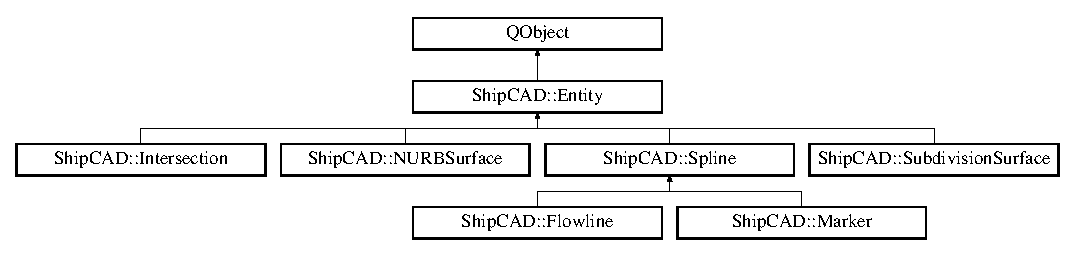
\includegraphics[height=2.978724cm]{classShipCAD_1_1Entity}
\end{center}
\end{figure}
\subsection*{Public Member Functions}
\begin{DoxyCompactItemize}
\item 
\hyperlink{classShipCAD_1_1Entity_a980f368aa07ce358583982821533a54a}{Entity} ()
\item 
virtual \hyperlink{classShipCAD_1_1Entity_a0fe3f9f7c8875a85afb214c8ebd75604}{$\sim$\+Entity} ()
\item 
virtual void \hyperlink{classShipCAD_1_1Entity_a998d0e5d360371046fd5835ba1e0877a}{clear} ()
\item 
virtual void \hyperlink{classShipCAD_1_1Entity_a08e8e53770c85002afa45f46e7bf10f8}{extents} (Q\+Vector3D \&min, Q\+Vector3D \&max)
\item 
virtual void \hyperlink{classShipCAD_1_1Entity_aa62e306d991140dcd564360f8f6e7539}{draw} (\hyperlink{classShipCAD_1_1Viewport}{Viewport} \&vp, \hyperlink{classShipCAD_1_1LineShader}{Line\+Shader} $\ast$lineshader)=0
\item 
virtual void \hyperlink{classShipCAD_1_1Entity_a2571654319df6ad6841a437be7a75395}{rebuild} ()=0
\item 
virtual Q\+Color \hyperlink{classShipCAD_1_1Entity_a747f437fa410f5b8b6251967fd3a90aa}{get\+Color} () const 
\item 
void \hyperlink{classShipCAD_1_1Entity_a5e0e5f174d287e807b5409b1aa5704bc}{set\+Color} (const Q\+Color \&col)
\item 
int \hyperlink{classShipCAD_1_1Entity_acf44d10747d8e1588030ef1e46155dfc}{get\+Pen\+Width} () const 
\item 
void \hyperlink{classShipCAD_1_1Entity_a1b8146f974735c90ea6a44a0cb5fba98}{set\+Pen\+Width} (int w)
\item 
Qt\+::\+Pen\+Style \hyperlink{classShipCAD_1_1Entity_a5912853854b82c79f47dd9117cc3d9bc}{get\+Pen\+Style} () const 
\item 
void \hyperlink{classShipCAD_1_1Entity_a50f556f934efd5517c984b09a2e17773}{set\+Pen\+Style} (Qt\+::\+Pen\+Style style)
\item 
Q\+Vector3D \hyperlink{classShipCAD_1_1Entity_a7c4227afa7a356a667224cfba69a24e5}{get\+Min} () const 
\item 
Q\+Vector3D \hyperlink{classShipCAD_1_1Entity_ad9e95df651ae01a48242604262b051b3}{get\+Max} () const 
\item 
bool \hyperlink{classShipCAD_1_1Entity_ab2f54a1745c95aa0871a8c57c114809e}{is\+Build} () const 
\item 
virtual void \hyperlink{classShipCAD_1_1Entity_a1889198398f42bb7f77a2334031c3f33}{set\+Build} (bool val)
\item 
void \hyperlink{classShipCAD_1_1Entity_a395d7573df06482d9deaecdc87d46944}{dump} (std\+::ostream \&os) const 
\end{DoxyCompactItemize}
\subsection*{Protected Attributes}
\begin{DoxyCompactItemize}
\item 
bool \hyperlink{classShipCAD_1_1Entity_a752e3eb309111a7457783e0fdab3d6fe}{\+\_\+build}
\item 
Q\+Vector3D \hyperlink{classShipCAD_1_1Entity_a414d4ff1ee308d47a5052910c3b34f7b}{\+\_\+min}
\item 
Q\+Vector3D \hyperlink{classShipCAD_1_1Entity_a30e4f9cb421987cebd07737a554275eb}{\+\_\+max}
\item 
int \hyperlink{classShipCAD_1_1Entity_a5a9892a0d84d2cfdcd3a5dabf662a595}{\+\_\+pen\+\_\+width}
\item 
Q\+Color \hyperlink{classShipCAD_1_1Entity_a150a19aa958886e9dcf7c4e0e51dcd98}{\+\_\+color}
\item 
Qt\+::\+Pen\+Style \hyperlink{classShipCAD_1_1Entity_ac53123be976cd9739ad1657573d67d97}{\+\_\+pen\+\_\+style}
\end{DoxyCompactItemize}


\subsection{Detailed Description}
base class for all non-\/surface drawable elements 

Definition at line 65 of file entity.\+h.



\subsection{Constructor \& Destructor Documentation}
\index{Ship\+C\+A\+D\+::\+Entity@{Ship\+C\+A\+D\+::\+Entity}!Entity@{Entity}}
\index{Entity@{Entity}!Ship\+C\+A\+D\+::\+Entity@{Ship\+C\+A\+D\+::\+Entity}}
\subsubsection[{\texorpdfstring{Entity()}{Entity()}}]{\setlength{\rightskip}{0pt plus 5cm}Entity\+::\+Entity (
\begin{DoxyParamCaption}
{}
\end{DoxyParamCaption}
)\hspace{0.3cm}{\ttfamily [explicit]}}\hypertarget{classShipCAD_1_1Entity_a980f368aa07ce358583982821533a54a}{}\label{classShipCAD_1_1Entity_a980f368aa07ce358583982821533a54a}


Definition at line 40 of file entity.\+cpp.

\index{Ship\+C\+A\+D\+::\+Entity@{Ship\+C\+A\+D\+::\+Entity}!````~Entity@{$\sim$\+Entity}}
\index{````~Entity@{$\sim$\+Entity}!Ship\+C\+A\+D\+::\+Entity@{Ship\+C\+A\+D\+::\+Entity}}
\subsubsection[{\texorpdfstring{$\sim$\+Entity()}{~Entity()}}]{\setlength{\rightskip}{0pt plus 5cm}virtual Ship\+C\+A\+D\+::\+Entity\+::$\sim$\+Entity (
\begin{DoxyParamCaption}
{}
\end{DoxyParamCaption}
)\hspace{0.3cm}{\ttfamily [inline]}, {\ttfamily [virtual]}}\hypertarget{classShipCAD_1_1Entity_a0fe3f9f7c8875a85afb214c8ebd75604}{}\label{classShipCAD_1_1Entity_a0fe3f9f7c8875a85afb214c8ebd75604}


Definition at line 72 of file entity.\+h.



\subsection{Member Function Documentation}
\index{Ship\+C\+A\+D\+::\+Entity@{Ship\+C\+A\+D\+::\+Entity}!clear@{clear}}
\index{clear@{clear}!Ship\+C\+A\+D\+::\+Entity@{Ship\+C\+A\+D\+::\+Entity}}
\subsubsection[{\texorpdfstring{clear()}{clear()}}]{\setlength{\rightskip}{0pt plus 5cm}void Entity\+::clear (
\begin{DoxyParamCaption}
{}
\end{DoxyParamCaption}
)\hspace{0.3cm}{\ttfamily [virtual]}}\hypertarget{classShipCAD_1_1Entity_a998d0e5d360371046fd5835ba1e0877a}{}\label{classShipCAD_1_1Entity_a998d0e5d360371046fd5835ba1e0877a}


Reimplemented in \hyperlink{classShipCAD_1_1SubdivisionSurface_a80ab3bd6372a8465d69f71034a353e06}{Ship\+C\+A\+D\+::\+Subdivision\+Surface}, \hyperlink{classShipCAD_1_1Spline_a02967f3eee8b1755eab0d7da55c3c621}{Ship\+C\+A\+D\+::\+Spline}, \hyperlink{classShipCAD_1_1Intersection_a2163245dc7153d1590811ab2902d6ee4}{Ship\+C\+A\+D\+::\+Intersection}, \hyperlink{classShipCAD_1_1Flowline_ac3bbbbd3d853214bb9c9feeb7a12314d}{Ship\+C\+A\+D\+::\+Flowline}, \hyperlink{classShipCAD_1_1Marker_ac7c7eea8648562f3fa00a9e10af6ec97}{Ship\+C\+A\+D\+::\+Marker}, and \hyperlink{classShipCAD_1_1NURBSurface_a5013b0c1e511ea68909eef5d0473d032}{Ship\+C\+A\+D\+::\+N\+U\+R\+B\+Surface}.



Definition at line 47 of file entity.\+cpp.

\index{Ship\+C\+A\+D\+::\+Entity@{Ship\+C\+A\+D\+::\+Entity}!draw@{draw}}
\index{draw@{draw}!Ship\+C\+A\+D\+::\+Entity@{Ship\+C\+A\+D\+::\+Entity}}
\subsubsection[{\texorpdfstring{draw(\+Viewport \&vp, Line\+Shader $\ast$lineshader)=0}{draw(Viewport &vp, LineShader *lineshader)=0}}]{\setlength{\rightskip}{0pt plus 5cm}virtual void Ship\+C\+A\+D\+::\+Entity\+::draw (
\begin{DoxyParamCaption}
\item[{{\bf Viewport} \&}]{vp, }
\item[{{\bf Line\+Shader} $\ast$}]{lineshader}
\end{DoxyParamCaption}
)\hspace{0.3cm}{\ttfamily [pure virtual]}}\hypertarget{classShipCAD_1_1Entity_aa62e306d991140dcd564360f8f6e7539}{}\label{classShipCAD_1_1Entity_aa62e306d991140dcd564360f8f6e7539}


Implemented in \hyperlink{classShipCAD_1_1SubdivisionSurface_ab1c250ff9fa7acae3ecdca4575f3e259}{Ship\+C\+A\+D\+::\+Subdivision\+Surface}, \hyperlink{classShipCAD_1_1Spline_a6424ed433d241f566c15891cc25a74dd}{Ship\+C\+A\+D\+::\+Spline}, \hyperlink{classShipCAD_1_1Intersection_a9e346019a52aa0540628b75994ea94a5}{Ship\+C\+A\+D\+::\+Intersection}, \hyperlink{classShipCAD_1_1Flowline_a8b43ac96514f62c6fb0db938eccd0d44}{Ship\+C\+A\+D\+::\+Flowline}, and \hyperlink{classShipCAD_1_1Marker_a0cca647d9b32dc69b03903b024dc3091}{Ship\+C\+A\+D\+::\+Marker}.

\index{Ship\+C\+A\+D\+::\+Entity@{Ship\+C\+A\+D\+::\+Entity}!dump@{dump}}
\index{dump@{dump}!Ship\+C\+A\+D\+::\+Entity@{Ship\+C\+A\+D\+::\+Entity}}
\subsubsection[{\texorpdfstring{dump(std\+::ostream \&os) const }{dump(std::ostream &os) const }}]{\setlength{\rightskip}{0pt plus 5cm}void Entity\+::dump (
\begin{DoxyParamCaption}
\item[{std\+::ostream \&}]{os}
\end{DoxyParamCaption}
) const}\hypertarget{classShipCAD_1_1Entity_a395d7573df06482d9deaecdc87d46944}{}\label{classShipCAD_1_1Entity_a395d7573df06482d9deaecdc87d46944}


Definition at line 90 of file entity.\+cpp.

\index{Ship\+C\+A\+D\+::\+Entity@{Ship\+C\+A\+D\+::\+Entity}!extents@{extents}}
\index{extents@{extents}!Ship\+C\+A\+D\+::\+Entity@{Ship\+C\+A\+D\+::\+Entity}}
\subsubsection[{\texorpdfstring{extents(\+Q\+Vector3\+D \&min, Q\+Vector3\+D \&max)}{extents(QVector3D &min, QVector3D &max)}}]{\setlength{\rightskip}{0pt plus 5cm}void Entity\+::extents (
\begin{DoxyParamCaption}
\item[{Q\+Vector3D \&}]{min, }
\item[{Q\+Vector3D \&}]{max}
\end{DoxyParamCaption}
)\hspace{0.3cm}{\ttfamily [virtual]}}\hypertarget{classShipCAD_1_1Entity_a08e8e53770c85002afa45f46e7bf10f8}{}\label{classShipCAD_1_1Entity_a08e8e53770c85002afa45f46e7bf10f8}


Reimplemented in \hyperlink{classShipCAD_1_1SubdivisionSurface_abc1cf0168290242dfbe5dd0d178fa7cb}{Ship\+C\+A\+D\+::\+Subdivision\+Surface}, and \hyperlink{classShipCAD_1_1Intersection_af751d515708531ca098321840a92c47b}{Ship\+C\+A\+D\+::\+Intersection}.



Definition at line 57 of file entity.\+cpp.

\index{Ship\+C\+A\+D\+::\+Entity@{Ship\+C\+A\+D\+::\+Entity}!get\+Color@{get\+Color}}
\index{get\+Color@{get\+Color}!Ship\+C\+A\+D\+::\+Entity@{Ship\+C\+A\+D\+::\+Entity}}
\subsubsection[{\texorpdfstring{get\+Color() const }{getColor() const }}]{\setlength{\rightskip}{0pt plus 5cm}virtual Q\+Color Ship\+C\+A\+D\+::\+Entity\+::get\+Color (
\begin{DoxyParamCaption}
{}
\end{DoxyParamCaption}
) const\hspace{0.3cm}{\ttfamily [inline]}, {\ttfamily [virtual]}}\hypertarget{classShipCAD_1_1Entity_a747f437fa410f5b8b6251967fd3a90aa}{}\label{classShipCAD_1_1Entity_a747f437fa410f5b8b6251967fd3a90aa}


Reimplemented in \hyperlink{classShipCAD_1_1Flowline_a546cee93d649cc3514bf2fcd19694ecf}{Ship\+C\+A\+D\+::\+Flowline}.



Definition at line 80 of file entity.\+h.

\index{Ship\+C\+A\+D\+::\+Entity@{Ship\+C\+A\+D\+::\+Entity}!get\+Max@{get\+Max}}
\index{get\+Max@{get\+Max}!Ship\+C\+A\+D\+::\+Entity@{Ship\+C\+A\+D\+::\+Entity}}
\subsubsection[{\texorpdfstring{get\+Max() const }{getMax() const }}]{\setlength{\rightskip}{0pt plus 5cm}Q\+Vector3D Entity\+::get\+Max (
\begin{DoxyParamCaption}
{}
\end{DoxyParamCaption}
) const}\hypertarget{classShipCAD_1_1Entity_ad9e95df651ae01a48242604262b051b3}{}\label{classShipCAD_1_1Entity_ad9e95df651ae01a48242604262b051b3}


Definition at line 83 of file entity.\+cpp.

\index{Ship\+C\+A\+D\+::\+Entity@{Ship\+C\+A\+D\+::\+Entity}!get\+Min@{get\+Min}}
\index{get\+Min@{get\+Min}!Ship\+C\+A\+D\+::\+Entity@{Ship\+C\+A\+D\+::\+Entity}}
\subsubsection[{\texorpdfstring{get\+Min() const }{getMin() const }}]{\setlength{\rightskip}{0pt plus 5cm}Q\+Vector3D Entity\+::get\+Min (
\begin{DoxyParamCaption}
{}
\end{DoxyParamCaption}
) const}\hypertarget{classShipCAD_1_1Entity_a7c4227afa7a356a667224cfba69a24e5}{}\label{classShipCAD_1_1Entity_a7c4227afa7a356a667224cfba69a24e5}


Definition at line 76 of file entity.\+cpp.

\index{Ship\+C\+A\+D\+::\+Entity@{Ship\+C\+A\+D\+::\+Entity}!get\+Pen\+Style@{get\+Pen\+Style}}
\index{get\+Pen\+Style@{get\+Pen\+Style}!Ship\+C\+A\+D\+::\+Entity@{Ship\+C\+A\+D\+::\+Entity}}
\subsubsection[{\texorpdfstring{get\+Pen\+Style() const }{getPenStyle() const }}]{\setlength{\rightskip}{0pt plus 5cm}Qt\+::\+Pen\+Style Ship\+C\+A\+D\+::\+Entity\+::get\+Pen\+Style (
\begin{DoxyParamCaption}
{}
\end{DoxyParamCaption}
) const\hspace{0.3cm}{\ttfamily [inline]}}\hypertarget{classShipCAD_1_1Entity_a5912853854b82c79f47dd9117cc3d9bc}{}\label{classShipCAD_1_1Entity_a5912853854b82c79f47dd9117cc3d9bc}


Definition at line 90 of file entity.\+h.

\index{Ship\+C\+A\+D\+::\+Entity@{Ship\+C\+A\+D\+::\+Entity}!get\+Pen\+Width@{get\+Pen\+Width}}
\index{get\+Pen\+Width@{get\+Pen\+Width}!Ship\+C\+A\+D\+::\+Entity@{Ship\+C\+A\+D\+::\+Entity}}
\subsubsection[{\texorpdfstring{get\+Pen\+Width() const }{getPenWidth() const }}]{\setlength{\rightskip}{0pt plus 5cm}int Ship\+C\+A\+D\+::\+Entity\+::get\+Pen\+Width (
\begin{DoxyParamCaption}
{}
\end{DoxyParamCaption}
) const\hspace{0.3cm}{\ttfamily [inline]}}\hypertarget{classShipCAD_1_1Entity_acf44d10747d8e1588030ef1e46155dfc}{}\label{classShipCAD_1_1Entity_acf44d10747d8e1588030ef1e46155dfc}


Definition at line 85 of file entity.\+h.

\index{Ship\+C\+A\+D\+::\+Entity@{Ship\+C\+A\+D\+::\+Entity}!is\+Build@{is\+Build}}
\index{is\+Build@{is\+Build}!Ship\+C\+A\+D\+::\+Entity@{Ship\+C\+A\+D\+::\+Entity}}
\subsubsection[{\texorpdfstring{is\+Build() const }{isBuild() const }}]{\setlength{\rightskip}{0pt plus 5cm}bool Ship\+C\+A\+D\+::\+Entity\+::is\+Build (
\begin{DoxyParamCaption}
{}
\end{DoxyParamCaption}
) const\hspace{0.3cm}{\ttfamily [inline]}}\hypertarget{classShipCAD_1_1Entity_ab2f54a1745c95aa0871a8c57c114809e}{}\label{classShipCAD_1_1Entity_ab2f54a1745c95aa0871a8c57c114809e}


Definition at line 97 of file entity.\+h.

\index{Ship\+C\+A\+D\+::\+Entity@{Ship\+C\+A\+D\+::\+Entity}!rebuild@{rebuild}}
\index{rebuild@{rebuild}!Ship\+C\+A\+D\+::\+Entity@{Ship\+C\+A\+D\+::\+Entity}}
\subsubsection[{\texorpdfstring{rebuild()=0}{rebuild()=0}}]{\setlength{\rightskip}{0pt plus 5cm}virtual void Ship\+C\+A\+D\+::\+Entity\+::rebuild (
\begin{DoxyParamCaption}
{}
\end{DoxyParamCaption}
)\hspace{0.3cm}{\ttfamily [pure virtual]}}\hypertarget{classShipCAD_1_1Entity_a2571654319df6ad6841a437be7a75395}{}\label{classShipCAD_1_1Entity_a2571654319df6ad6841a437be7a75395}


Implemented in \hyperlink{classShipCAD_1_1SubdivisionSurface_a259856fc21f2bc1eebbc52f10dd59469}{Ship\+C\+A\+D\+::\+Subdivision\+Surface}, \hyperlink{classShipCAD_1_1Spline_a9b466ad7510032dafb0421f2d834bde6}{Ship\+C\+A\+D\+::\+Spline}, \hyperlink{classShipCAD_1_1Intersection_aed30bdca43037f72b85c4d53e234fd6c}{Ship\+C\+A\+D\+::\+Intersection}, \hyperlink{classShipCAD_1_1Flowline_a28e5d73316c6d2c8005428669a9e9b97}{Ship\+C\+A\+D\+::\+Flowline}, and \hyperlink{classShipCAD_1_1NURBSurface_a643231ea9a8f26e528a1d9a0dccf4070}{Ship\+C\+A\+D\+::\+N\+U\+R\+B\+Surface}.

\index{Ship\+C\+A\+D\+::\+Entity@{Ship\+C\+A\+D\+::\+Entity}!set\+Build@{set\+Build}}
\index{set\+Build@{set\+Build}!Ship\+C\+A\+D\+::\+Entity@{Ship\+C\+A\+D\+::\+Entity}}
\subsubsection[{\texorpdfstring{set\+Build(bool val)}{setBuild(bool val)}}]{\setlength{\rightskip}{0pt plus 5cm}void Entity\+::set\+Build (
\begin{DoxyParamCaption}
\item[{bool}]{val}
\end{DoxyParamCaption}
)\hspace{0.3cm}{\ttfamily [virtual]}}\hypertarget{classShipCAD_1_1Entity_a1889198398f42bb7f77a2334031c3f33}{}\label{classShipCAD_1_1Entity_a1889198398f42bb7f77a2334031c3f33}


Reimplemented in \hyperlink{classShipCAD_1_1SubdivisionSurface_aec5073750762d1f8c3ab2107a742f4a5}{Ship\+C\+A\+D\+::\+Subdivision\+Surface}, \hyperlink{classShipCAD_1_1Spline_a6e932411f0f4463514f80011c58f5e6a}{Ship\+C\+A\+D\+::\+Spline}, \hyperlink{classShipCAD_1_1Intersection_a2b496f9ab21c5fc4a7b97a665b24f2b1}{Ship\+C\+A\+D\+::\+Intersection}, \hyperlink{classShipCAD_1_1NURBSurface_aa6fc3d060087593349ce1b5119419433}{Ship\+C\+A\+D\+::\+N\+U\+R\+B\+Surface}, and \hyperlink{classShipCAD_1_1Flowline_ad148400a3e53b2368b37c2c7f50ec1b7}{Ship\+C\+A\+D\+::\+Flowline}.



Definition at line 65 of file entity.\+cpp.

\index{Ship\+C\+A\+D\+::\+Entity@{Ship\+C\+A\+D\+::\+Entity}!set\+Color@{set\+Color}}
\index{set\+Color@{set\+Color}!Ship\+C\+A\+D\+::\+Entity@{Ship\+C\+A\+D\+::\+Entity}}
\subsubsection[{\texorpdfstring{set\+Color(const Q\+Color \&col)}{setColor(const QColor &col)}}]{\setlength{\rightskip}{0pt plus 5cm}void Ship\+C\+A\+D\+::\+Entity\+::set\+Color (
\begin{DoxyParamCaption}
\item[{const Q\+Color \&}]{col}
\end{DoxyParamCaption}
)\hspace{0.3cm}{\ttfamily [inline]}}\hypertarget{classShipCAD_1_1Entity_a5e0e5f174d287e807b5409b1aa5704bc}{}\label{classShipCAD_1_1Entity_a5e0e5f174d287e807b5409b1aa5704bc}


Definition at line 82 of file entity.\+h.

\index{Ship\+C\+A\+D\+::\+Entity@{Ship\+C\+A\+D\+::\+Entity}!set\+Pen\+Style@{set\+Pen\+Style}}
\index{set\+Pen\+Style@{set\+Pen\+Style}!Ship\+C\+A\+D\+::\+Entity@{Ship\+C\+A\+D\+::\+Entity}}
\subsubsection[{\texorpdfstring{set\+Pen\+Style(\+Qt\+::\+Pen\+Style style)}{setPenStyle(Qt::PenStyle style)}}]{\setlength{\rightskip}{0pt plus 5cm}void Ship\+C\+A\+D\+::\+Entity\+::set\+Pen\+Style (
\begin{DoxyParamCaption}
\item[{Qt\+::\+Pen\+Style}]{style}
\end{DoxyParamCaption}
)\hspace{0.3cm}{\ttfamily [inline]}}\hypertarget{classShipCAD_1_1Entity_a50f556f934efd5517c984b09a2e17773}{}\label{classShipCAD_1_1Entity_a50f556f934efd5517c984b09a2e17773}


Definition at line 92 of file entity.\+h.

\index{Ship\+C\+A\+D\+::\+Entity@{Ship\+C\+A\+D\+::\+Entity}!set\+Pen\+Width@{set\+Pen\+Width}}
\index{set\+Pen\+Width@{set\+Pen\+Width}!Ship\+C\+A\+D\+::\+Entity@{Ship\+C\+A\+D\+::\+Entity}}
\subsubsection[{\texorpdfstring{set\+Pen\+Width(int w)}{setPenWidth(int w)}}]{\setlength{\rightskip}{0pt plus 5cm}void Ship\+C\+A\+D\+::\+Entity\+::set\+Pen\+Width (
\begin{DoxyParamCaption}
\item[{int}]{w}
\end{DoxyParamCaption}
)\hspace{0.3cm}{\ttfamily [inline]}}\hypertarget{classShipCAD_1_1Entity_a1b8146f974735c90ea6a44a0cb5fba98}{}\label{classShipCAD_1_1Entity_a1b8146f974735c90ea6a44a0cb5fba98}


Definition at line 87 of file entity.\+h.



\subsection{Member Data Documentation}
\index{Ship\+C\+A\+D\+::\+Entity@{Ship\+C\+A\+D\+::\+Entity}!\+\_\+build@{\+\_\+build}}
\index{\+\_\+build@{\+\_\+build}!Ship\+C\+A\+D\+::\+Entity@{Ship\+C\+A\+D\+::\+Entity}}
\subsubsection[{\texorpdfstring{\+\_\+build}{_build}}]{\setlength{\rightskip}{0pt plus 5cm}bool Ship\+C\+A\+D\+::\+Entity\+::\+\_\+build\hspace{0.3cm}{\ttfamily [protected]}}\hypertarget{classShipCAD_1_1Entity_a752e3eb309111a7457783e0fdab3d6fe}{}\label{classShipCAD_1_1Entity_a752e3eb309111a7457783e0fdab3d6fe}


Definition at line 108 of file entity.\+h.

\index{Ship\+C\+A\+D\+::\+Entity@{Ship\+C\+A\+D\+::\+Entity}!\+\_\+color@{\+\_\+color}}
\index{\+\_\+color@{\+\_\+color}!Ship\+C\+A\+D\+::\+Entity@{Ship\+C\+A\+D\+::\+Entity}}
\subsubsection[{\texorpdfstring{\+\_\+color}{_color}}]{\setlength{\rightskip}{0pt plus 5cm}Q\+Color Ship\+C\+A\+D\+::\+Entity\+::\+\_\+color\hspace{0.3cm}{\ttfamily [protected]}}\hypertarget{classShipCAD_1_1Entity_a150a19aa958886e9dcf7c4e0e51dcd98}{}\label{classShipCAD_1_1Entity_a150a19aa958886e9dcf7c4e0e51dcd98}


Definition at line 112 of file entity.\+h.

\index{Ship\+C\+A\+D\+::\+Entity@{Ship\+C\+A\+D\+::\+Entity}!\+\_\+max@{\+\_\+max}}
\index{\+\_\+max@{\+\_\+max}!Ship\+C\+A\+D\+::\+Entity@{Ship\+C\+A\+D\+::\+Entity}}
\subsubsection[{\texorpdfstring{\+\_\+max}{_max}}]{\setlength{\rightskip}{0pt plus 5cm}Q\+Vector3D Ship\+C\+A\+D\+::\+Entity\+::\+\_\+max\hspace{0.3cm}{\ttfamily [protected]}}\hypertarget{classShipCAD_1_1Entity_a30e4f9cb421987cebd07737a554275eb}{}\label{classShipCAD_1_1Entity_a30e4f9cb421987cebd07737a554275eb}


Definition at line 110 of file entity.\+h.

\index{Ship\+C\+A\+D\+::\+Entity@{Ship\+C\+A\+D\+::\+Entity}!\+\_\+min@{\+\_\+min}}
\index{\+\_\+min@{\+\_\+min}!Ship\+C\+A\+D\+::\+Entity@{Ship\+C\+A\+D\+::\+Entity}}
\subsubsection[{\texorpdfstring{\+\_\+min}{_min}}]{\setlength{\rightskip}{0pt plus 5cm}Q\+Vector3D Ship\+C\+A\+D\+::\+Entity\+::\+\_\+min\hspace{0.3cm}{\ttfamily [protected]}}\hypertarget{classShipCAD_1_1Entity_a414d4ff1ee308d47a5052910c3b34f7b}{}\label{classShipCAD_1_1Entity_a414d4ff1ee308d47a5052910c3b34f7b}


Definition at line 109 of file entity.\+h.

\index{Ship\+C\+A\+D\+::\+Entity@{Ship\+C\+A\+D\+::\+Entity}!\+\_\+pen\+\_\+style@{\+\_\+pen\+\_\+style}}
\index{\+\_\+pen\+\_\+style@{\+\_\+pen\+\_\+style}!Ship\+C\+A\+D\+::\+Entity@{Ship\+C\+A\+D\+::\+Entity}}
\subsubsection[{\texorpdfstring{\+\_\+pen\+\_\+style}{_pen_style}}]{\setlength{\rightskip}{0pt plus 5cm}Qt\+::\+Pen\+Style Ship\+C\+A\+D\+::\+Entity\+::\+\_\+pen\+\_\+style\hspace{0.3cm}{\ttfamily [protected]}}\hypertarget{classShipCAD_1_1Entity_ac53123be976cd9739ad1657573d67d97}{}\label{classShipCAD_1_1Entity_ac53123be976cd9739ad1657573d67d97}


Definition at line 113 of file entity.\+h.

\index{Ship\+C\+A\+D\+::\+Entity@{Ship\+C\+A\+D\+::\+Entity}!\+\_\+pen\+\_\+width@{\+\_\+pen\+\_\+width}}
\index{\+\_\+pen\+\_\+width@{\+\_\+pen\+\_\+width}!Ship\+C\+A\+D\+::\+Entity@{Ship\+C\+A\+D\+::\+Entity}}
\subsubsection[{\texorpdfstring{\+\_\+pen\+\_\+width}{_pen_width}}]{\setlength{\rightskip}{0pt plus 5cm}int Ship\+C\+A\+D\+::\+Entity\+::\+\_\+pen\+\_\+width\hspace{0.3cm}{\ttfamily [protected]}}\hypertarget{classShipCAD_1_1Entity_a5a9892a0d84d2cfdcd3a5dabf662a595}{}\label{classShipCAD_1_1Entity_a5a9892a0d84d2cfdcd3a5dabf662a595}


Definition at line 111 of file entity.\+h.



The documentation for this class was generated from the following files\+:\begin{DoxyCompactItemize}
\item 
Ship\+C\+A\+Dlib/\hyperlink{entity_8h}{entity.\+h}\item 
Ship\+C\+A\+Dlib/\hyperlink{entity_8cpp}{entity.\+cpp}\end{DoxyCompactItemize}

\hypertarget{structShipCAD_1_1ExtrudeEdgeDialogData}{}\section{Ship\+C\+AD\+:\+:Extrude\+Edge\+Dialog\+Data Struct Reference}
\label{structShipCAD_1_1ExtrudeEdgeDialogData}\index{Ship\+C\+A\+D\+::\+Extrude\+Edge\+Dialog\+Data@{Ship\+C\+A\+D\+::\+Extrude\+Edge\+Dialog\+Data}}


extrude edge dialog exchange  




{\ttfamily \#include $<$dialogdata.\+h$>$}

\subsection*{Public Member Functions}
\begin{DoxyCompactItemize}
\item 
\hyperlink{structShipCAD_1_1ExtrudeEdgeDialogData_a412fc868ad680d1d418ea16d9dbbfed1}{Extrude\+Edge\+Dialog\+Data} ()
\end{DoxyCompactItemize}
\subsection*{Public Attributes}
\begin{DoxyCompactItemize}
\item 
bool \hyperlink{structShipCAD_1_1ExtrudeEdgeDialogData_acacc5c53abda4c79c30f52d96de6d1f9}{accepted}
\item 
Q\+Vector3D \hyperlink{structShipCAD_1_1ExtrudeEdgeDialogData_aa1841a8d73ac4887e46f3f2d0712770c}{vector}
\end{DoxyCompactItemize}


\subsection{Detailed Description}
extrude edge dialog exchange 

Definition at line 69 of file dialogdata.\+h.



\subsection{Constructor \& Destructor Documentation}
\index{Ship\+C\+A\+D\+::\+Extrude\+Edge\+Dialog\+Data@{Ship\+C\+A\+D\+::\+Extrude\+Edge\+Dialog\+Data}!Extrude\+Edge\+Dialog\+Data@{Extrude\+Edge\+Dialog\+Data}}
\index{Extrude\+Edge\+Dialog\+Data@{Extrude\+Edge\+Dialog\+Data}!Ship\+C\+A\+D\+::\+Extrude\+Edge\+Dialog\+Data@{Ship\+C\+A\+D\+::\+Extrude\+Edge\+Dialog\+Data}}
\subsubsection[{\texorpdfstring{Extrude\+Edge\+Dialog\+Data()}{ExtrudeEdgeDialogData()}}]{\setlength{\rightskip}{0pt plus 5cm}Extrude\+Edge\+Dialog\+Data\+::\+Extrude\+Edge\+Dialog\+Data (
\begin{DoxyParamCaption}
{}
\end{DoxyParamCaption}
)\hspace{0.3cm}{\ttfamily [explicit]}}\hypertarget{structShipCAD_1_1ExtrudeEdgeDialogData_a412fc868ad680d1d418ea16d9dbbfed1}{}\label{structShipCAD_1_1ExtrudeEdgeDialogData_a412fc868ad680d1d418ea16d9dbbfed1}


Definition at line 43 of file dialogdata.\+cpp.



\subsection{Member Data Documentation}
\index{Ship\+C\+A\+D\+::\+Extrude\+Edge\+Dialog\+Data@{Ship\+C\+A\+D\+::\+Extrude\+Edge\+Dialog\+Data}!accepted@{accepted}}
\index{accepted@{accepted}!Ship\+C\+A\+D\+::\+Extrude\+Edge\+Dialog\+Data@{Ship\+C\+A\+D\+::\+Extrude\+Edge\+Dialog\+Data}}
\subsubsection[{\texorpdfstring{accepted}{accepted}}]{\setlength{\rightskip}{0pt plus 5cm}bool Ship\+C\+A\+D\+::\+Extrude\+Edge\+Dialog\+Data\+::accepted}\hypertarget{structShipCAD_1_1ExtrudeEdgeDialogData_acacc5c53abda4c79c30f52d96de6d1f9}{}\label{structShipCAD_1_1ExtrudeEdgeDialogData_acacc5c53abda4c79c30f52d96de6d1f9}


Definition at line 71 of file dialogdata.\+h.

\index{Ship\+C\+A\+D\+::\+Extrude\+Edge\+Dialog\+Data@{Ship\+C\+A\+D\+::\+Extrude\+Edge\+Dialog\+Data}!vector@{vector}}
\index{vector@{vector}!Ship\+C\+A\+D\+::\+Extrude\+Edge\+Dialog\+Data@{Ship\+C\+A\+D\+::\+Extrude\+Edge\+Dialog\+Data}}
\subsubsection[{\texorpdfstring{vector}{vector}}]{\setlength{\rightskip}{0pt plus 5cm}Q\+Vector3D Ship\+C\+A\+D\+::\+Extrude\+Edge\+Dialog\+Data\+::vector}\hypertarget{structShipCAD_1_1ExtrudeEdgeDialogData_aa1841a8d73ac4887e46f3f2d0712770c}{}\label{structShipCAD_1_1ExtrudeEdgeDialogData_aa1841a8d73ac4887e46f3f2d0712770c}


Definition at line 72 of file dialogdata.\+h.



The documentation for this struct was generated from the following files\+:\begin{DoxyCompactItemize}
\item 
Ship\+C\+A\+Dlib/\hyperlink{dialogdata_8h}{dialogdata.\+h}\item 
Ship\+C\+A\+Dlib/\hyperlink{dialogdata_8cpp}{dialogdata.\+cpp}\end{DoxyCompactItemize}

\hypertarget{classShipCAD_1_1FaceShader}{}\section{Ship\+C\+AD\+:\+:Face\+Shader Class Reference}
\label{classShipCAD_1_1FaceShader}\index{Ship\+C\+A\+D\+::\+Face\+Shader@{Ship\+C\+A\+D\+::\+Face\+Shader}}


{\ttfamily \#include $<$shader.\+h$>$}

Inheritance diagram for Ship\+C\+AD\+:\+:Face\+Shader\+:\begin{figure}[H]
\begin{center}
\leavevmode
\includegraphics[height=4.000000cm]{classShipCAD_1_1FaceShader}
\end{center}
\end{figure}
\subsection*{Public Member Functions}
\begin{DoxyCompactItemize}
\item 
\hyperlink{classShipCAD_1_1FaceShader_a67bd0296f829456035a829b95f1befb7}{Face\+Shader} (\hyperlink{classShipCAD_1_1Viewport}{Viewport} $\ast$vp)
\item 
virtual \hyperlink{classShipCAD_1_1FaceShader_afbd21e69afb094aea484144be9ac1fbd}{$\sim$\+Face\+Shader} ()
\item 
virtual void \hyperlink{classShipCAD_1_1FaceShader_adb71f051d1481058fe905f985a7166c1}{render\+Mesh} (Q\+Color mesh\+Color, Q\+Vector$<$ Q\+Vector3D $>$ \&vertices, Q\+Vector$<$ Q\+Vector3D $>$ \&normals)=0
\end{DoxyCompactItemize}
\subsection*{Additional Inherited Members}


\subsection{Detailed Description}


Definition at line 97 of file shader.\+h.



\subsection{Constructor \& Destructor Documentation}
\index{Ship\+C\+A\+D\+::\+Face\+Shader@{Ship\+C\+A\+D\+::\+Face\+Shader}!Face\+Shader@{Face\+Shader}}
\index{Face\+Shader@{Face\+Shader}!Ship\+C\+A\+D\+::\+Face\+Shader@{Ship\+C\+A\+D\+::\+Face\+Shader}}
\subsubsection[{\texorpdfstring{Face\+Shader(\+Viewport $\ast$vp)}{FaceShader(Viewport *vp)}}]{\setlength{\rightskip}{0pt plus 5cm}Ship\+C\+A\+D\+::\+Face\+Shader\+::\+Face\+Shader (
\begin{DoxyParamCaption}
\item[{{\bf Viewport} $\ast$}]{vp}
\end{DoxyParamCaption}
)\hspace{0.3cm}{\ttfamily [inline]}, {\ttfamily [explicit]}}\hypertarget{classShipCAD_1_1FaceShader_a67bd0296f829456035a829b95f1befb7}{}\label{classShipCAD_1_1FaceShader_a67bd0296f829456035a829b95f1befb7}


Definition at line 103 of file shader.\+h.

\index{Ship\+C\+A\+D\+::\+Face\+Shader@{Ship\+C\+A\+D\+::\+Face\+Shader}!````~Face\+Shader@{$\sim$\+Face\+Shader}}
\index{````~Face\+Shader@{$\sim$\+Face\+Shader}!Ship\+C\+A\+D\+::\+Face\+Shader@{Ship\+C\+A\+D\+::\+Face\+Shader}}
\subsubsection[{\texorpdfstring{$\sim$\+Face\+Shader()}{~FaceShader()}}]{\setlength{\rightskip}{0pt plus 5cm}virtual Ship\+C\+A\+D\+::\+Face\+Shader\+::$\sim$\+Face\+Shader (
\begin{DoxyParamCaption}
{}
\end{DoxyParamCaption}
)\hspace{0.3cm}{\ttfamily [inline]}, {\ttfamily [virtual]}}\hypertarget{classShipCAD_1_1FaceShader_afbd21e69afb094aea484144be9ac1fbd}{}\label{classShipCAD_1_1FaceShader_afbd21e69afb094aea484144be9ac1fbd}


Definition at line 105 of file shader.\+h.



\subsection{Member Function Documentation}
\index{Ship\+C\+A\+D\+::\+Face\+Shader@{Ship\+C\+A\+D\+::\+Face\+Shader}!render\+Mesh@{render\+Mesh}}
\index{render\+Mesh@{render\+Mesh}!Ship\+C\+A\+D\+::\+Face\+Shader@{Ship\+C\+A\+D\+::\+Face\+Shader}}
\subsubsection[{\texorpdfstring{render\+Mesh(\+Q\+Color mesh\+Color, Q\+Vector$<$ Q\+Vector3\+D $>$ \&vertices, Q\+Vector$<$ Q\+Vector3\+D $>$ \&normals)=0}{renderMesh(QColor meshColor, QVector< QVector3D > &vertices, QVector< QVector3D > &normals)=0}}]{\setlength{\rightskip}{0pt plus 5cm}virtual void Ship\+C\+A\+D\+::\+Face\+Shader\+::render\+Mesh (
\begin{DoxyParamCaption}
\item[{Q\+Color}]{mesh\+Color, }
\item[{Q\+Vector$<$ Q\+Vector3D $>$ \&}]{vertices, }
\item[{Q\+Vector$<$ Q\+Vector3D $>$ \&}]{normals}
\end{DoxyParamCaption}
)\hspace{0.3cm}{\ttfamily [pure virtual]}}\hypertarget{classShipCAD_1_1FaceShader_adb71f051d1481058fe905f985a7166c1}{}\label{classShipCAD_1_1FaceShader_adb71f051d1481058fe905f985a7166c1}


Implemented in \hyperlink{classShipCAD_1_1LightedFaceShader_abd4fe9c01a7e09aa46f3017f014018a8}{Ship\+C\+A\+D\+::\+Lighted\+Face\+Shader}, and \hyperlink{classShipCAD_1_1MonoFaceShader_a9a358ec63af4b067449e772cbc735d5a}{Ship\+C\+A\+D\+::\+Mono\+Face\+Shader}.



The documentation for this class was generated from the following file\+:\begin{DoxyCompactItemize}
\item 
Ship\+C\+A\+Dlib/\hyperlink{shader_8h}{shader.\+h}\end{DoxyCompactItemize}

\hypertarget{classShipCAD_1_1FileBuffer}{}\section{Ship\+C\+AD\+:\+:File\+Buffer Class Reference}
\label{classShipCAD_1_1FileBuffer}\index{Ship\+C\+A\+D\+::\+File\+Buffer@{Ship\+C\+A\+D\+::\+File\+Buffer}}


in-\/memory buffer for a binary file (F\+R\+E\+E!\+Ship format)  




{\ttfamily \#include $<$filebuffer.\+h$>$}

Inheritance diagram for Ship\+C\+AD\+:\+:File\+Buffer\+:\begin{figure}[H]
\begin{center}
\leavevmode
\includegraphics[height=2.000000cm]{classShipCAD_1_1FileBuffer}
\end{center}
\end{figure}
\subsection*{Public Member Functions}
\begin{DoxyCompactItemize}
\item 
\hyperlink{classShipCAD_1_1FileBuffer_ab243cfcb8a68ce791103594e974ee9ba}{File\+Buffer} ()
\item 
\hyperlink{classShipCAD_1_1FileBuffer_a397c9a755598f9939eb30460b605d44c}{$\sim$\+File\+Buffer} ()
\item 
size\+\_\+t \hyperlink{classShipCAD_1_1FileBuffer_a51dc1007457d999ce374afd6a6ae29f8}{size} ()
\item 
size\+\_\+t \hyperlink{classShipCAD_1_1FileBuffer_a7feeac3f68df96065a3238cbca9a5151}{pos} ()
\item 
\hyperlink{namespaceShipCAD_af3a6fa23a7318acbda7b0066b53d694f}{version\+\_\+t} \hyperlink{classShipCAD_1_1FileBuffer_a06f87b30f5fd091cc5c270964ea16770}{get\+Version} ()
\item 
void \hyperlink{classShipCAD_1_1FileBuffer_a66c14f8f21b9f77febd154aee9565f0b}{set\+Version} (\hyperlink{namespaceShipCAD_af3a6fa23a7318acbda7b0066b53d694f}{version\+\_\+t} v)
\item 
void \hyperlink{classShipCAD_1_1FileBuffer_afe2a6e56770eed6bf9df894baa28c9fe}{load\+From\+File} (Q\+File \&file)
\item 
void \hyperlink{classShipCAD_1_1FileBuffer_adcc7e54a07f39ad930df82da9c3c70fd}{save\+To\+File} (Q\+File \&file)
\item 
void \hyperlink{classShipCAD_1_1FileBuffer_af59c26297994b38aabc4bc678d04c246}{reset} ()
\item 
void \hyperlink{classShipCAD_1_1FileBuffer_a86223c54bcf111ef205c9d651e0b9a66}{load} (\hyperlink{structShipCAD_1_1JPEGImage}{J\+P\+E\+G\+Image} \&img)
\item 
void \hyperlink{classShipCAD_1_1FileBuffer_a9a5d46b2c6d568ee2cdef110d4773e73}{add} (const \hyperlink{structShipCAD_1_1JPEGImage}{J\+P\+E\+G\+Image} \&img)
\item 
void \hyperlink{classShipCAD_1_1FileBuffer_ab196d459581b5c877ebea2f567e9bda8}{load} (quint8 \&val)
\item 
void \hyperlink{classShipCAD_1_1FileBuffer_afb11c583e5d3a7a580e5f88004d6c7e3}{add} (quint8 val)
\item 
void \hyperlink{classShipCAD_1_1FileBuffer_ad1aebcc97e364569934c66eec5a87485}{load} (bool \&val)
\item 
void \hyperlink{classShipCAD_1_1FileBuffer_a7cb4395eae7ffa405290c3bed9890bee}{add} (bool val)
\item 
void \hyperlink{classShipCAD_1_1FileBuffer_a525306d68a017ef67ec13c3e8901a8ff}{load} (float \&val)
\item 
void \hyperlink{classShipCAD_1_1FileBuffer_a7909794ac33ad5f695bb670940db99ba}{add} (float val)
\item 
void \hyperlink{classShipCAD_1_1FileBuffer_ad7fc82d31f73f0350715fb63db2fc271}{load} (qint32 \&val)
\item 
void \hyperlink{classShipCAD_1_1FileBuffer_ad5ff9b7299df09feb365250c69e6da9a}{add} (qint32 val)
\item 
void \hyperlink{classShipCAD_1_1FileBuffer_a19fcd1363671552150de3d6ee3297f2c}{load} (quint32 \&val)
\item 
void \hyperlink{classShipCAD_1_1FileBuffer_a1dd1963dd35caff15333f21cc2195b34}{add} (quint32 val)
\item 
void \hyperlink{classShipCAD_1_1FileBuffer_aa22983fa24559f6d0d119d89036100af}{add} (size\+\_\+t val)
\begin{DoxyCompactList}\small\item\em save value, (check that it fits in 32 bits) \end{DoxyCompactList}\item 
void \hyperlink{classShipCAD_1_1FileBuffer_a7255342a053689ebafda9317cc586c57}{load} (Q\+Vector3D \&val)
\item 
void \hyperlink{classShipCAD_1_1FileBuffer_a0642733d14682981c12f6aeaef9bb884}{add} (const Q\+Vector3D \&val)
\item 
void \hyperlink{classShipCAD_1_1FileBuffer_a3329cf81740c79967acc24bc0ac3c9a3}{load} (Q\+Color \&val)
\item 
void \hyperlink{classShipCAD_1_1FileBuffer_a3611327a77cc938e987ecda018d0d936}{add} (const Q\+Color \&val)
\item 
void \hyperlink{classShipCAD_1_1FileBuffer_a82c790d09c8e85c0f9d218efd9c93605}{load} (Q\+String \&val)
\item 
void \hyperlink{classShipCAD_1_1FileBuffer_aea305be34bc316cc5b849fb291499012}{add} (const Q\+String \&val)
\item 
void \hyperlink{classShipCAD_1_1FileBuffer_ab266512b0703e4e62a32cbbcc4dd7050}{add} (const char $\ast$str)
\item 
void \hyperlink{classShipCAD_1_1FileBuffer_a4ae77da0ea26a1ed6de262ff7f3d606f}{load} (\hyperlink{classShipCAD_1_1Plane}{Plane} \&val)
\item 
void \hyperlink{classShipCAD_1_1FileBuffer_ae947c5bac13749a8b0d833bfa7979d0d}{add} (const \hyperlink{classShipCAD_1_1Plane}{Plane} \&val)
\item 
void \hyperlink{classShipCAD_1_1FileBuffer_acfa1ad9b776baa948d1724bd56b4e18d}{load} (\hyperlink{structShipCAD_1_1DelftSeriesResistance}{Delft\+Series\+Resistance} $\ast$buf)
\item 
void \hyperlink{classShipCAD_1_1FileBuffer_a63b2793d04b55d67ef7a307e664b3416}{add} (const \hyperlink{structShipCAD_1_1DelftSeriesResistance}{Delft\+Series\+Resistance} $\ast$buf)
\item 
void \hyperlink{classShipCAD_1_1FileBuffer_aec2753a3f1fb3aab1303a8dfde26bb1c}{load} (\hyperlink{structShipCAD_1_1KAPERResistance}{K\+A\+P\+E\+R\+Resistance} $\ast$buf)
\item 
void \hyperlink{classShipCAD_1_1FileBuffer_a1189100c2022918351d730590d107c33}{add} (const \hyperlink{structShipCAD_1_1KAPERResistance}{K\+A\+P\+E\+R\+Resistance} $\ast$buf)
\end{DoxyCompactItemize}


\subsection{Detailed Description}
in-\/memory buffer for a binary file (F\+R\+E\+E!\+Ship format) 

Definition at line 52 of file filebuffer.\+h.



\subsection{Constructor \& Destructor Documentation}
\index{Ship\+C\+A\+D\+::\+File\+Buffer@{Ship\+C\+A\+D\+::\+File\+Buffer}!File\+Buffer@{File\+Buffer}}
\index{File\+Buffer@{File\+Buffer}!Ship\+C\+A\+D\+::\+File\+Buffer@{Ship\+C\+A\+D\+::\+File\+Buffer}}
\subsubsection[{\texorpdfstring{File\+Buffer()}{FileBuffer()}}]{\setlength{\rightskip}{0pt plus 5cm}File\+Buffer\+::\+File\+Buffer (
\begin{DoxyParamCaption}
{}
\end{DoxyParamCaption}
)\hspace{0.3cm}{\ttfamily [explicit]}}\hypertarget{classShipCAD_1_1FileBuffer_ab243cfcb8a68ce791103594e974ee9ba}{}\label{classShipCAD_1_1FileBuffer_ab243cfcb8a68ce791103594e974ee9ba}


Definition at line 52 of file filebuffer.\+cpp.

\index{Ship\+C\+A\+D\+::\+File\+Buffer@{Ship\+C\+A\+D\+::\+File\+Buffer}!````~File\+Buffer@{$\sim$\+File\+Buffer}}
\index{````~File\+Buffer@{$\sim$\+File\+Buffer}!Ship\+C\+A\+D\+::\+File\+Buffer@{Ship\+C\+A\+D\+::\+File\+Buffer}}
\subsubsection[{\texorpdfstring{$\sim$\+File\+Buffer()}{~FileBuffer()}}]{\setlength{\rightskip}{0pt plus 5cm}Ship\+C\+A\+D\+::\+File\+Buffer\+::$\sim$\+File\+Buffer (
\begin{DoxyParamCaption}
{}
\end{DoxyParamCaption}
)\hspace{0.3cm}{\ttfamily [inline]}}\hypertarget{classShipCAD_1_1FileBuffer_a397c9a755598f9939eb30460b605d44c}{}\label{classShipCAD_1_1FileBuffer_a397c9a755598f9939eb30460b605d44c}


Definition at line 58 of file filebuffer.\+h.



\subsection{Member Function Documentation}
\index{Ship\+C\+A\+D\+::\+File\+Buffer@{Ship\+C\+A\+D\+::\+File\+Buffer}!add@{add}}
\index{add@{add}!Ship\+C\+A\+D\+::\+File\+Buffer@{Ship\+C\+A\+D\+::\+File\+Buffer}}
\subsubsection[{\texorpdfstring{add(const J\+P\+E\+G\+Image \&img)}{add(const JPEGImage &img)}}]{\setlength{\rightskip}{0pt plus 5cm}void File\+Buffer\+::add (
\begin{DoxyParamCaption}
\item[{const {\bf J\+P\+E\+G\+Image} \&}]{img}
\end{DoxyParamCaption}
)}\hypertarget{classShipCAD_1_1FileBuffer_a9a5d46b2c6d568ee2cdef110d4773e73}{}\label{classShipCAD_1_1FileBuffer_a9a5d46b2c6d568ee2cdef110d4773e73}


Definition at line 108 of file filebuffer.\+cpp.

\index{Ship\+C\+A\+D\+::\+File\+Buffer@{Ship\+C\+A\+D\+::\+File\+Buffer}!add@{add}}
\index{add@{add}!Ship\+C\+A\+D\+::\+File\+Buffer@{Ship\+C\+A\+D\+::\+File\+Buffer}}
\subsubsection[{\texorpdfstring{add(quint8 val)}{add(quint8 val)}}]{\setlength{\rightskip}{0pt plus 5cm}void File\+Buffer\+::add (
\begin{DoxyParamCaption}
\item[{quint8}]{val}
\end{DoxyParamCaption}
)}\hypertarget{classShipCAD_1_1FileBuffer_afb11c583e5d3a7a580e5f88004d6c7e3}{}\label{classShipCAD_1_1FileBuffer_afb11c583e5d3a7a580e5f88004d6c7e3}


Definition at line 123 of file filebuffer.\+cpp.

\index{Ship\+C\+A\+D\+::\+File\+Buffer@{Ship\+C\+A\+D\+::\+File\+Buffer}!add@{add}}
\index{add@{add}!Ship\+C\+A\+D\+::\+File\+Buffer@{Ship\+C\+A\+D\+::\+File\+Buffer}}
\subsubsection[{\texorpdfstring{add(bool val)}{add(bool val)}}]{\setlength{\rightskip}{0pt plus 5cm}void File\+Buffer\+::add (
\begin{DoxyParamCaption}
\item[{bool}]{val}
\end{DoxyParamCaption}
)}\hypertarget{classShipCAD_1_1FileBuffer_a7cb4395eae7ffa405290c3bed9890bee}{}\label{classShipCAD_1_1FileBuffer_a7cb4395eae7ffa405290c3bed9890bee}


Definition at line 136 of file filebuffer.\+cpp.

\index{Ship\+C\+A\+D\+::\+File\+Buffer@{Ship\+C\+A\+D\+::\+File\+Buffer}!add@{add}}
\index{add@{add}!Ship\+C\+A\+D\+::\+File\+Buffer@{Ship\+C\+A\+D\+::\+File\+Buffer}}
\subsubsection[{\texorpdfstring{add(float val)}{add(float val)}}]{\setlength{\rightskip}{0pt plus 5cm}void File\+Buffer\+::add (
\begin{DoxyParamCaption}
\item[{float}]{val}
\end{DoxyParamCaption}
)}\hypertarget{classShipCAD_1_1FileBuffer_a7909794ac33ad5f695bb670940db99ba}{}\label{classShipCAD_1_1FileBuffer_a7909794ac33ad5f695bb670940db99ba}


Definition at line 150 of file filebuffer.\+cpp.

\index{Ship\+C\+A\+D\+::\+File\+Buffer@{Ship\+C\+A\+D\+::\+File\+Buffer}!add@{add}}
\index{add@{add}!Ship\+C\+A\+D\+::\+File\+Buffer@{Ship\+C\+A\+D\+::\+File\+Buffer}}
\subsubsection[{\texorpdfstring{add(qint32 val)}{add(qint32 val)}}]{\setlength{\rightskip}{0pt plus 5cm}void File\+Buffer\+::add (
\begin{DoxyParamCaption}
\item[{qint32}]{val}
\end{DoxyParamCaption}
)}\hypertarget{classShipCAD_1_1FileBuffer_ad5ff9b7299df09feb365250c69e6da9a}{}\label{classShipCAD_1_1FileBuffer_ad5ff9b7299df09feb365250c69e6da9a}


Definition at line 167 of file filebuffer.\+cpp.

\index{Ship\+C\+A\+D\+::\+File\+Buffer@{Ship\+C\+A\+D\+::\+File\+Buffer}!add@{add}}
\index{add@{add}!Ship\+C\+A\+D\+::\+File\+Buffer@{Ship\+C\+A\+D\+::\+File\+Buffer}}
\subsubsection[{\texorpdfstring{add(quint32 val)}{add(quint32 val)}}]{\setlength{\rightskip}{0pt plus 5cm}void File\+Buffer\+::add (
\begin{DoxyParamCaption}
\item[{quint32}]{val}
\end{DoxyParamCaption}
)}\hypertarget{classShipCAD_1_1FileBuffer_a1dd1963dd35caff15333f21cc2195b34}{}\label{classShipCAD_1_1FileBuffer_a1dd1963dd35caff15333f21cc2195b34}


Definition at line 184 of file filebuffer.\+cpp.

\index{Ship\+C\+A\+D\+::\+File\+Buffer@{Ship\+C\+A\+D\+::\+File\+Buffer}!add@{add}}
\index{add@{add}!Ship\+C\+A\+D\+::\+File\+Buffer@{Ship\+C\+A\+D\+::\+File\+Buffer}}
\subsubsection[{\texorpdfstring{add(size\+\_\+t val)}{add(size_t val)}}]{\setlength{\rightskip}{0pt plus 5cm}void File\+Buffer\+::add (
\begin{DoxyParamCaption}
\item[{size\+\_\+t}]{val}
\end{DoxyParamCaption}
)}\hypertarget{classShipCAD_1_1FileBuffer_aa22983fa24559f6d0d119d89036100af}{}\label{classShipCAD_1_1FileBuffer_aa22983fa24559f6d0d119d89036100af}


save value, (check that it fits in 32 bits) 


\begin{DoxyParams}{Parameters}
{\em val} & integer to save \\
\hline
\end{DoxyParams}

\begin{DoxyExceptions}{Exceptions}
{\em range\+\_\+error} & if val is greater than 32bit unsigned \\
\hline
\end{DoxyExceptions}


Definition at line 193 of file filebuffer.\+cpp.

\index{Ship\+C\+A\+D\+::\+File\+Buffer@{Ship\+C\+A\+D\+::\+File\+Buffer}!add@{add}}
\index{add@{add}!Ship\+C\+A\+D\+::\+File\+Buffer@{Ship\+C\+A\+D\+::\+File\+Buffer}}
\subsubsection[{\texorpdfstring{add(const Q\+Vector3\+D \&val)}{add(const QVector3D &val)}}]{\setlength{\rightskip}{0pt plus 5cm}void File\+Buffer\+::add (
\begin{DoxyParamCaption}
\item[{const Q\+Vector3D \&}]{val}
\end{DoxyParamCaption}
)}\hypertarget{classShipCAD_1_1FileBuffer_a0642733d14682981c12f6aeaef9bb884}{}\label{classShipCAD_1_1FileBuffer_a0642733d14682981c12f6aeaef9bb884}


Definition at line 237 of file filebuffer.\+cpp.

\index{Ship\+C\+A\+D\+::\+File\+Buffer@{Ship\+C\+A\+D\+::\+File\+Buffer}!add@{add}}
\index{add@{add}!Ship\+C\+A\+D\+::\+File\+Buffer@{Ship\+C\+A\+D\+::\+File\+Buffer}}
\subsubsection[{\texorpdfstring{add(const Q\+Color \&val)}{add(const QColor &val)}}]{\setlength{\rightskip}{0pt plus 5cm}void File\+Buffer\+::add (
\begin{DoxyParamCaption}
\item[{const Q\+Color \&}]{val}
\end{DoxyParamCaption}
)}\hypertarget{classShipCAD_1_1FileBuffer_a3611327a77cc938e987ecda018d0d936}{}\label{classShipCAD_1_1FileBuffer_a3611327a77cc938e987ecda018d0d936}


Definition at line 204 of file filebuffer.\+cpp.

\index{Ship\+C\+A\+D\+::\+File\+Buffer@{Ship\+C\+A\+D\+::\+File\+Buffer}!add@{add}}
\index{add@{add}!Ship\+C\+A\+D\+::\+File\+Buffer@{Ship\+C\+A\+D\+::\+File\+Buffer}}
\subsubsection[{\texorpdfstring{add(const Q\+String \&val)}{add(const QString &val)}}]{\setlength{\rightskip}{0pt plus 5cm}void File\+Buffer\+::add (
\begin{DoxyParamCaption}
\item[{const Q\+String \&}]{val}
\end{DoxyParamCaption}
)}\hypertarget{classShipCAD_1_1FileBuffer_aea305be34bc316cc5b849fb291499012}{}\label{classShipCAD_1_1FileBuffer_aea305be34bc316cc5b849fb291499012}


Definition at line 266 of file filebuffer.\+cpp.

\index{Ship\+C\+A\+D\+::\+File\+Buffer@{Ship\+C\+A\+D\+::\+File\+Buffer}!add@{add}}
\index{add@{add}!Ship\+C\+A\+D\+::\+File\+Buffer@{Ship\+C\+A\+D\+::\+File\+Buffer}}
\subsubsection[{\texorpdfstring{add(const char $\ast$str)}{add(const char *str)}}]{\setlength{\rightskip}{0pt plus 5cm}void File\+Buffer\+::add (
\begin{DoxyParamCaption}
\item[{const char $\ast$}]{str}
\end{DoxyParamCaption}
)}\hypertarget{classShipCAD_1_1FileBuffer_ab266512b0703e4e62a32cbbcc4dd7050}{}\label{classShipCAD_1_1FileBuffer_ab266512b0703e4e62a32cbbcc4dd7050}


Definition at line 278 of file filebuffer.\+cpp.

\index{Ship\+C\+A\+D\+::\+File\+Buffer@{Ship\+C\+A\+D\+::\+File\+Buffer}!add@{add}}
\index{add@{add}!Ship\+C\+A\+D\+::\+File\+Buffer@{Ship\+C\+A\+D\+::\+File\+Buffer}}
\subsubsection[{\texorpdfstring{add(const Plane \&val)}{add(const Plane &val)}}]{\setlength{\rightskip}{0pt plus 5cm}void File\+Buffer\+::add (
\begin{DoxyParamCaption}
\item[{const {\bf Plane} \&}]{val}
\end{DoxyParamCaption}
)}\hypertarget{classShipCAD_1_1FileBuffer_ae947c5bac13749a8b0d833bfa7979d0d}{}\label{classShipCAD_1_1FileBuffer_ae947c5bac13749a8b0d833bfa7979d0d}


Definition at line 309 of file filebuffer.\+cpp.

\index{Ship\+C\+A\+D\+::\+File\+Buffer@{Ship\+C\+A\+D\+::\+File\+Buffer}!add@{add}}
\index{add@{add}!Ship\+C\+A\+D\+::\+File\+Buffer@{Ship\+C\+A\+D\+::\+File\+Buffer}}
\subsubsection[{\texorpdfstring{add(const Delft\+Series\+Resistance $\ast$buf)}{add(const DelftSeriesResistance *buf)}}]{\setlength{\rightskip}{0pt plus 5cm}void File\+Buffer\+::add (
\begin{DoxyParamCaption}
\item[{const {\bf Delft\+Series\+Resistance} $\ast$}]{buf}
\end{DoxyParamCaption}
)}\hypertarget{classShipCAD_1_1FileBuffer_a63b2793d04b55d67ef7a307e664b3416}{}\label{classShipCAD_1_1FileBuffer_a63b2793d04b55d67ef7a307e664b3416}


Definition at line 334 of file filebuffer.\+cpp.

\index{Ship\+C\+A\+D\+::\+File\+Buffer@{Ship\+C\+A\+D\+::\+File\+Buffer}!add@{add}}
\index{add@{add}!Ship\+C\+A\+D\+::\+File\+Buffer@{Ship\+C\+A\+D\+::\+File\+Buffer}}
\subsubsection[{\texorpdfstring{add(const K\+A\+P\+E\+R\+Resistance $\ast$buf)}{add(const KAPERResistance *buf)}}]{\setlength{\rightskip}{0pt plus 5cm}void File\+Buffer\+::add (
\begin{DoxyParamCaption}
\item[{const {\bf K\+A\+P\+E\+R\+Resistance} $\ast$}]{buf}
\end{DoxyParamCaption}
)}\hypertarget{classShipCAD_1_1FileBuffer_a1189100c2022918351d730590d107c33}{}\label{classShipCAD_1_1FileBuffer_a1189100c2022918351d730590d107c33}


Definition at line 349 of file filebuffer.\+cpp.

\index{Ship\+C\+A\+D\+::\+File\+Buffer@{Ship\+C\+A\+D\+::\+File\+Buffer}!get\+Version@{get\+Version}}
\index{get\+Version@{get\+Version}!Ship\+C\+A\+D\+::\+File\+Buffer@{Ship\+C\+A\+D\+::\+File\+Buffer}}
\subsubsection[{\texorpdfstring{get\+Version()}{getVersion()}}]{\setlength{\rightskip}{0pt plus 5cm}{\bf version\+\_\+t} Ship\+C\+A\+D\+::\+File\+Buffer\+::get\+Version (
\begin{DoxyParamCaption}
{}
\end{DoxyParamCaption}
)\hspace{0.3cm}{\ttfamily [inline]}}\hypertarget{classShipCAD_1_1FileBuffer_a06f87b30f5fd091cc5c270964ea16770}{}\label{classShipCAD_1_1FileBuffer_a06f87b30f5fd091cc5c270964ea16770}


Definition at line 64 of file filebuffer.\+h.

\index{Ship\+C\+A\+D\+::\+File\+Buffer@{Ship\+C\+A\+D\+::\+File\+Buffer}!load@{load}}
\index{load@{load}!Ship\+C\+A\+D\+::\+File\+Buffer@{Ship\+C\+A\+D\+::\+File\+Buffer}}
\subsubsection[{\texorpdfstring{load(\+J\+P\+E\+G\+Image \&img)}{load(JPEGImage &img)}}]{\setlength{\rightskip}{0pt plus 5cm}void File\+Buffer\+::load (
\begin{DoxyParamCaption}
\item[{{\bf J\+P\+E\+G\+Image} \&}]{img}
\end{DoxyParamCaption}
)}\hypertarget{classShipCAD_1_1FileBuffer_a86223c54bcf111ef205c9d651e0b9a66}{}\label{classShipCAD_1_1FileBuffer_a86223c54bcf111ef205c9d651e0b9a66}


Definition at line 96 of file filebuffer.\+cpp.

\index{Ship\+C\+A\+D\+::\+File\+Buffer@{Ship\+C\+A\+D\+::\+File\+Buffer}!load@{load}}
\index{load@{load}!Ship\+C\+A\+D\+::\+File\+Buffer@{Ship\+C\+A\+D\+::\+File\+Buffer}}
\subsubsection[{\texorpdfstring{load(quint8 \&val)}{load(quint8 &val)}}]{\setlength{\rightskip}{0pt plus 5cm}void File\+Buffer\+::load (
\begin{DoxyParamCaption}
\item[{quint8 \&}]{val}
\end{DoxyParamCaption}
)}\hypertarget{classShipCAD_1_1FileBuffer_ab196d459581b5c877ebea2f567e9bda8}{}\label{classShipCAD_1_1FileBuffer_ab196d459581b5c877ebea2f567e9bda8}


Definition at line 117 of file filebuffer.\+cpp.

\index{Ship\+C\+A\+D\+::\+File\+Buffer@{Ship\+C\+A\+D\+::\+File\+Buffer}!load@{load}}
\index{load@{load}!Ship\+C\+A\+D\+::\+File\+Buffer@{Ship\+C\+A\+D\+::\+File\+Buffer}}
\subsubsection[{\texorpdfstring{load(bool \&val)}{load(bool &val)}}]{\setlength{\rightskip}{0pt plus 5cm}void File\+Buffer\+::load (
\begin{DoxyParamCaption}
\item[{bool \&}]{val}
\end{DoxyParamCaption}
)}\hypertarget{classShipCAD_1_1FileBuffer_ad1aebcc97e364569934c66eec5a87485}{}\label{classShipCAD_1_1FileBuffer_ad1aebcc97e364569934c66eec5a87485}


Definition at line 128 of file filebuffer.\+cpp.

\index{Ship\+C\+A\+D\+::\+File\+Buffer@{Ship\+C\+A\+D\+::\+File\+Buffer}!load@{load}}
\index{load@{load}!Ship\+C\+A\+D\+::\+File\+Buffer@{Ship\+C\+A\+D\+::\+File\+Buffer}}
\subsubsection[{\texorpdfstring{load(float \&val)}{load(float &val)}}]{\setlength{\rightskip}{0pt plus 5cm}void File\+Buffer\+::load (
\begin{DoxyParamCaption}
\item[{float \&}]{val}
\end{DoxyParamCaption}
)}\hypertarget{classShipCAD_1_1FileBuffer_a525306d68a017ef67ec13c3e8901a8ff}{}\label{classShipCAD_1_1FileBuffer_a525306d68a017ef67ec13c3e8901a8ff}


Definition at line 141 of file filebuffer.\+cpp.

\index{Ship\+C\+A\+D\+::\+File\+Buffer@{Ship\+C\+A\+D\+::\+File\+Buffer}!load@{load}}
\index{load@{load}!Ship\+C\+A\+D\+::\+File\+Buffer@{Ship\+C\+A\+D\+::\+File\+Buffer}}
\subsubsection[{\texorpdfstring{load(qint32 \&val)}{load(qint32 &val)}}]{\setlength{\rightskip}{0pt plus 5cm}void File\+Buffer\+::load (
\begin{DoxyParamCaption}
\item[{qint32 \&}]{val}
\end{DoxyParamCaption}
)}\hypertarget{classShipCAD_1_1FileBuffer_ad7fc82d31f73f0350715fb63db2fc271}{}\label{classShipCAD_1_1FileBuffer_ad7fc82d31f73f0350715fb63db2fc271}


Definition at line 158 of file filebuffer.\+cpp.

\index{Ship\+C\+A\+D\+::\+File\+Buffer@{Ship\+C\+A\+D\+::\+File\+Buffer}!load@{load}}
\index{load@{load}!Ship\+C\+A\+D\+::\+File\+Buffer@{Ship\+C\+A\+D\+::\+File\+Buffer}}
\subsubsection[{\texorpdfstring{load(quint32 \&val)}{load(quint32 &val)}}]{\setlength{\rightskip}{0pt plus 5cm}void File\+Buffer\+::load (
\begin{DoxyParamCaption}
\item[{quint32 \&}]{val}
\end{DoxyParamCaption}
)}\hypertarget{classShipCAD_1_1FileBuffer_a19fcd1363671552150de3d6ee3297f2c}{}\label{classShipCAD_1_1FileBuffer_a19fcd1363671552150de3d6ee3297f2c}


Definition at line 175 of file filebuffer.\+cpp.

\index{Ship\+C\+A\+D\+::\+File\+Buffer@{Ship\+C\+A\+D\+::\+File\+Buffer}!load@{load}}
\index{load@{load}!Ship\+C\+A\+D\+::\+File\+Buffer@{Ship\+C\+A\+D\+::\+File\+Buffer}}
\subsubsection[{\texorpdfstring{load(\+Q\+Vector3\+D \&val)}{load(QVector3D &val)}}]{\setlength{\rightskip}{0pt plus 5cm}void File\+Buffer\+::load (
\begin{DoxyParamCaption}
\item[{Q\+Vector3D \&}]{val}
\end{DoxyParamCaption}
)}\hypertarget{classShipCAD_1_1FileBuffer_a7255342a053689ebafda9317cc586c57}{}\label{classShipCAD_1_1FileBuffer_a7255342a053689ebafda9317cc586c57}


Definition at line 222 of file filebuffer.\+cpp.

\index{Ship\+C\+A\+D\+::\+File\+Buffer@{Ship\+C\+A\+D\+::\+File\+Buffer}!load@{load}}
\index{load@{load}!Ship\+C\+A\+D\+::\+File\+Buffer@{Ship\+C\+A\+D\+::\+File\+Buffer}}
\subsubsection[{\texorpdfstring{load(\+Q\+Color \&val)}{load(QColor &val)}}]{\setlength{\rightskip}{0pt plus 5cm}void File\+Buffer\+::load (
\begin{DoxyParamCaption}
\item[{Q\+Color \&}]{val}
\end{DoxyParamCaption}
)}\hypertarget{classShipCAD_1_1FileBuffer_a3329cf81740c79967acc24bc0ac3c9a3}{}\label{classShipCAD_1_1FileBuffer_a3329cf81740c79967acc24bc0ac3c9a3}


Definition at line 212 of file filebuffer.\+cpp.

\index{Ship\+C\+A\+D\+::\+File\+Buffer@{Ship\+C\+A\+D\+::\+File\+Buffer}!load@{load}}
\index{load@{load}!Ship\+C\+A\+D\+::\+File\+Buffer@{Ship\+C\+A\+D\+::\+File\+Buffer}}
\subsubsection[{\texorpdfstring{load(\+Q\+String \&val)}{load(QString &val)}}]{\setlength{\rightskip}{0pt plus 5cm}void File\+Buffer\+::load (
\begin{DoxyParamCaption}
\item[{Q\+String \&}]{val}
\end{DoxyParamCaption}
)}\hypertarget{classShipCAD_1_1FileBuffer_a82c790d09c8e85c0f9d218efd9c93605}{}\label{classShipCAD_1_1FileBuffer_a82c790d09c8e85c0f9d218efd9c93605}


Definition at line 251 of file filebuffer.\+cpp.

\index{Ship\+C\+A\+D\+::\+File\+Buffer@{Ship\+C\+A\+D\+::\+File\+Buffer}!load@{load}}
\index{load@{load}!Ship\+C\+A\+D\+::\+File\+Buffer@{Ship\+C\+A\+D\+::\+File\+Buffer}}
\subsubsection[{\texorpdfstring{load(\+Plane \&val)}{load(Plane &val)}}]{\setlength{\rightskip}{0pt plus 5cm}void File\+Buffer\+::load (
\begin{DoxyParamCaption}
\item[{{\bf Plane} \&}]{val}
\end{DoxyParamCaption}
)}\hypertarget{classShipCAD_1_1FileBuffer_a4ae77da0ea26a1ed6de262ff7f3d606f}{}\label{classShipCAD_1_1FileBuffer_a4ae77da0ea26a1ed6de262ff7f3d606f}


Definition at line 291 of file filebuffer.\+cpp.

\index{Ship\+C\+A\+D\+::\+File\+Buffer@{Ship\+C\+A\+D\+::\+File\+Buffer}!load@{load}}
\index{load@{load}!Ship\+C\+A\+D\+::\+File\+Buffer@{Ship\+C\+A\+D\+::\+File\+Buffer}}
\subsubsection[{\texorpdfstring{load(\+Delft\+Series\+Resistance $\ast$buf)}{load(DelftSeriesResistance *buf)}}]{\setlength{\rightskip}{0pt plus 5cm}void File\+Buffer\+::load (
\begin{DoxyParamCaption}
\item[{{\bf Delft\+Series\+Resistance} $\ast$}]{buf}
\end{DoxyParamCaption}
)}\hypertarget{classShipCAD_1_1FileBuffer_acfa1ad9b776baa948d1724bd56b4e18d}{}\label{classShipCAD_1_1FileBuffer_acfa1ad9b776baa948d1724bd56b4e18d}


Definition at line 326 of file filebuffer.\+cpp.

\index{Ship\+C\+A\+D\+::\+File\+Buffer@{Ship\+C\+A\+D\+::\+File\+Buffer}!load@{load}}
\index{load@{load}!Ship\+C\+A\+D\+::\+File\+Buffer@{Ship\+C\+A\+D\+::\+File\+Buffer}}
\subsubsection[{\texorpdfstring{load(\+K\+A\+P\+E\+R\+Resistance $\ast$buf)}{load(KAPERResistance *buf)}}]{\setlength{\rightskip}{0pt plus 5cm}void File\+Buffer\+::load (
\begin{DoxyParamCaption}
\item[{{\bf K\+A\+P\+E\+R\+Resistance} $\ast$}]{buf}
\end{DoxyParamCaption}
)}\hypertarget{classShipCAD_1_1FileBuffer_aec2753a3f1fb3aab1303a8dfde26bb1c}{}\label{classShipCAD_1_1FileBuffer_aec2753a3f1fb3aab1303a8dfde26bb1c}


Definition at line 341 of file filebuffer.\+cpp.

\index{Ship\+C\+A\+D\+::\+File\+Buffer@{Ship\+C\+A\+D\+::\+File\+Buffer}!load\+From\+File@{load\+From\+File}}
\index{load\+From\+File@{load\+From\+File}!Ship\+C\+A\+D\+::\+File\+Buffer@{Ship\+C\+A\+D\+::\+File\+Buffer}}
\subsubsection[{\texorpdfstring{load\+From\+File(\+Q\+File \&file)}{loadFromFile(QFile &file)}}]{\setlength{\rightskip}{0pt plus 5cm}void File\+Buffer\+::load\+From\+File (
\begin{DoxyParamCaption}
\item[{Q\+File \&}]{file}
\end{DoxyParamCaption}
)}\hypertarget{classShipCAD_1_1FileBuffer_afe2a6e56770eed6bf9df894baa28c9fe}{}\label{classShipCAD_1_1FileBuffer_afe2a6e56770eed6bf9df894baa28c9fe}


Definition at line 68 of file filebuffer.\+cpp.

\index{Ship\+C\+A\+D\+::\+File\+Buffer@{Ship\+C\+A\+D\+::\+File\+Buffer}!pos@{pos}}
\index{pos@{pos}!Ship\+C\+A\+D\+::\+File\+Buffer@{Ship\+C\+A\+D\+::\+File\+Buffer}}
\subsubsection[{\texorpdfstring{pos()}{pos()}}]{\setlength{\rightskip}{0pt plus 5cm}size\+\_\+t Ship\+C\+A\+D\+::\+File\+Buffer\+::pos (
\begin{DoxyParamCaption}
{}
\end{DoxyParamCaption}
)\hspace{0.3cm}{\ttfamily [inline]}}\hypertarget{classShipCAD_1_1FileBuffer_a7feeac3f68df96065a3238cbca9a5151}{}\label{classShipCAD_1_1FileBuffer_a7feeac3f68df96065a3238cbca9a5151}


Definition at line 61 of file filebuffer.\+h.

\index{Ship\+C\+A\+D\+::\+File\+Buffer@{Ship\+C\+A\+D\+::\+File\+Buffer}!reset@{reset}}
\index{reset@{reset}!Ship\+C\+A\+D\+::\+File\+Buffer@{Ship\+C\+A\+D\+::\+File\+Buffer}}
\subsubsection[{\texorpdfstring{reset()}{reset()}}]{\setlength{\rightskip}{0pt plus 5cm}void File\+Buffer\+::reset (
\begin{DoxyParamCaption}
{}
\end{DoxyParamCaption}
)}\hypertarget{classShipCAD_1_1FileBuffer_af59c26297994b38aabc4bc678d04c246}{}\label{classShipCAD_1_1FileBuffer_af59c26297994b38aabc4bc678d04c246}


Definition at line 58 of file filebuffer.\+cpp.

\index{Ship\+C\+A\+D\+::\+File\+Buffer@{Ship\+C\+A\+D\+::\+File\+Buffer}!save\+To\+File@{save\+To\+File}}
\index{save\+To\+File@{save\+To\+File}!Ship\+C\+A\+D\+::\+File\+Buffer@{Ship\+C\+A\+D\+::\+File\+Buffer}}
\subsubsection[{\texorpdfstring{save\+To\+File(\+Q\+File \&file)}{saveToFile(QFile &file)}}]{\setlength{\rightskip}{0pt plus 5cm}void File\+Buffer\+::save\+To\+File (
\begin{DoxyParamCaption}
\item[{Q\+File \&}]{file}
\end{DoxyParamCaption}
)}\hypertarget{classShipCAD_1_1FileBuffer_adcc7e54a07f39ad930df82da9c3c70fd}{}\label{classShipCAD_1_1FileBuffer_adcc7e54a07f39ad930df82da9c3c70fd}


Definition at line 85 of file filebuffer.\+cpp.

\index{Ship\+C\+A\+D\+::\+File\+Buffer@{Ship\+C\+A\+D\+::\+File\+Buffer}!set\+Version@{set\+Version}}
\index{set\+Version@{set\+Version}!Ship\+C\+A\+D\+::\+File\+Buffer@{Ship\+C\+A\+D\+::\+File\+Buffer}}
\subsubsection[{\texorpdfstring{set\+Version(version\+\_\+t v)}{setVersion(version_t v)}}]{\setlength{\rightskip}{0pt plus 5cm}void File\+Buffer\+::set\+Version (
\begin{DoxyParamCaption}
\item[{{\bf version\+\_\+t}}]{v}
\end{DoxyParamCaption}
)}\hypertarget{classShipCAD_1_1FileBuffer_a66c14f8f21b9f77febd154aee9565f0b}{}\label{classShipCAD_1_1FileBuffer_a66c14f8f21b9f77febd154aee9565f0b}


Definition at line 63 of file filebuffer.\+cpp.

\index{Ship\+C\+A\+D\+::\+File\+Buffer@{Ship\+C\+A\+D\+::\+File\+Buffer}!size@{size}}
\index{size@{size}!Ship\+C\+A\+D\+::\+File\+Buffer@{Ship\+C\+A\+D\+::\+File\+Buffer}}
\subsubsection[{\texorpdfstring{size()}{size()}}]{\setlength{\rightskip}{0pt plus 5cm}size\+\_\+t Ship\+C\+A\+D\+::\+File\+Buffer\+::size (
\begin{DoxyParamCaption}
{}
\end{DoxyParamCaption}
)\hspace{0.3cm}{\ttfamily [inline]}}\hypertarget{classShipCAD_1_1FileBuffer_a51dc1007457d999ce374afd6a6ae29f8}{}\label{classShipCAD_1_1FileBuffer_a51dc1007457d999ce374afd6a6ae29f8}


Definition at line 60 of file filebuffer.\+h.



The documentation for this class was generated from the following files\+:\begin{DoxyCompactItemize}
\item 
Ship\+C\+A\+Dlib/\hyperlink{filebuffer_8h}{filebuffer.\+h}\item 
Ship\+C\+A\+Dlib/\hyperlink{filebuffer_8cpp}{filebuffer.\+cpp}\end{DoxyCompactItemize}

\hypertarget{classShipCAD_1_1FileReadError}{}\section{Ship\+C\+AD\+:\+:File\+Read\+Error Class Reference}
\label{classShipCAD_1_1FileReadError}\index{Ship\+C\+A\+D\+::\+File\+Read\+Error@{Ship\+C\+A\+D\+::\+File\+Read\+Error}}


{\ttfamily \#include $<$exception.\+h$>$}

Inheritance diagram for Ship\+C\+AD\+:\+:File\+Read\+Error\+:\begin{figure}[H]
\begin{center}
\leavevmode
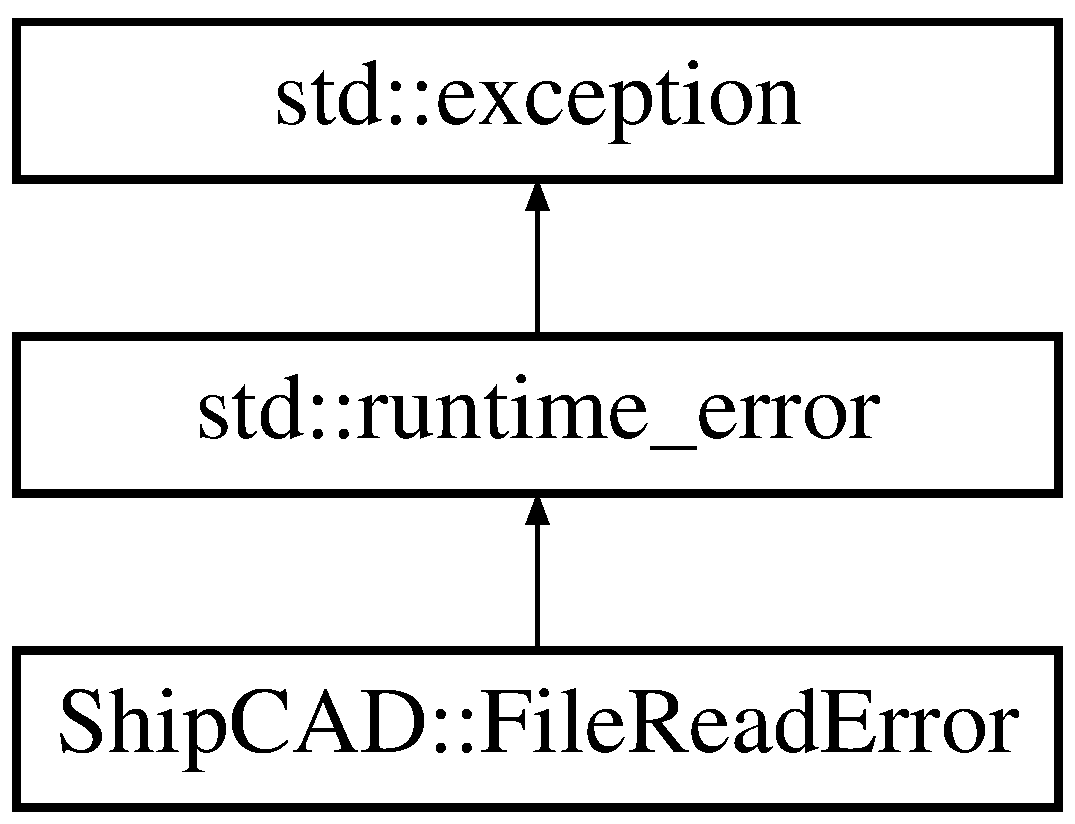
\includegraphics[height=3.000000cm]{classShipCAD_1_1FileReadError}
\end{center}
\end{figure}
\subsection*{Public Member Functions}
\begin{DoxyCompactItemize}
\item 
\hyperlink{classShipCAD_1_1FileReadError_af4660ee1297c946d3a3d62b83b0f9641}{File\+Read\+Error} (const Q\+String \&\hyperlink{classShipCAD_1_1FileReadError_a53b6474345c764fb85faa24eb9713a56}{info})
\item 
const Q\+String \& \hyperlink{classShipCAD_1_1FileReadError_a53b6474345c764fb85faa24eb9713a56}{info} () const 
\end{DoxyCompactItemize}


\subsection{Detailed Description}


Definition at line 65 of file exception.\+h.



\subsection{Constructor \& Destructor Documentation}
\index{Ship\+C\+A\+D\+::\+File\+Read\+Error@{Ship\+C\+A\+D\+::\+File\+Read\+Error}!File\+Read\+Error@{File\+Read\+Error}}
\index{File\+Read\+Error@{File\+Read\+Error}!Ship\+C\+A\+D\+::\+File\+Read\+Error@{Ship\+C\+A\+D\+::\+File\+Read\+Error}}
\subsubsection[{\texorpdfstring{File\+Read\+Error(const Q\+String \&info)}{FileReadError(const QString &info)}}]{\setlength{\rightskip}{0pt plus 5cm}Ship\+C\+A\+D\+::\+File\+Read\+Error\+::\+File\+Read\+Error (
\begin{DoxyParamCaption}
\item[{const Q\+String \&}]{info}
\end{DoxyParamCaption}
)\hspace{0.3cm}{\ttfamily [inline]}}\hypertarget{classShipCAD_1_1FileReadError_af4660ee1297c946d3a3d62b83b0f9641}{}\label{classShipCAD_1_1FileReadError_af4660ee1297c946d3a3d62b83b0f9641}


Definition at line 68 of file exception.\+h.



\subsection{Member Function Documentation}
\index{Ship\+C\+A\+D\+::\+File\+Read\+Error@{Ship\+C\+A\+D\+::\+File\+Read\+Error}!info@{info}}
\index{info@{info}!Ship\+C\+A\+D\+::\+File\+Read\+Error@{Ship\+C\+A\+D\+::\+File\+Read\+Error}}
\subsubsection[{\texorpdfstring{info() const }{info() const }}]{\setlength{\rightskip}{0pt plus 5cm}const Q\+String\& Ship\+C\+A\+D\+::\+File\+Read\+Error\+::info (
\begin{DoxyParamCaption}
{}
\end{DoxyParamCaption}
) const\hspace{0.3cm}{\ttfamily [inline]}}\hypertarget{classShipCAD_1_1FileReadError_a53b6474345c764fb85faa24eb9713a56}{}\label{classShipCAD_1_1FileReadError_a53b6474345c764fb85faa24eb9713a56}


Definition at line 71 of file exception.\+h.



The documentation for this class was generated from the following file\+:\begin{DoxyCompactItemize}
\item 
Ship\+C\+A\+Dlib/\hyperlink{exception_8h}{exception.\+h}\end{DoxyCompactItemize}

\hypertarget{classShipCAD_1_1FileSaveError}{}\section{Ship\+C\+AD\+:\+:File\+Save\+Error Class Reference}
\label{classShipCAD_1_1FileSaveError}\index{Ship\+C\+A\+D\+::\+File\+Save\+Error@{Ship\+C\+A\+D\+::\+File\+Save\+Error}}


{\ttfamily \#include $<$exception.\+h$>$}

Inheritance diagram for Ship\+C\+AD\+:\+:File\+Save\+Error\+:\begin{figure}[H]
\begin{center}
\leavevmode
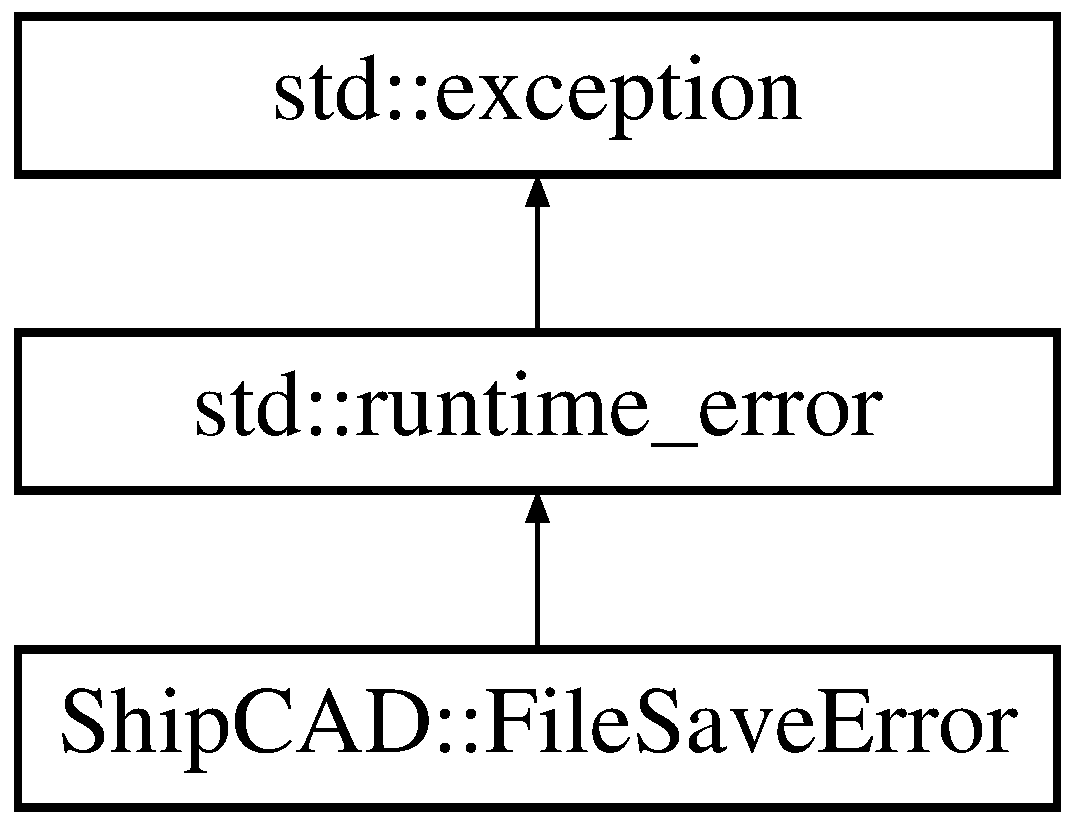
\includegraphics[height=3.000000cm]{classShipCAD_1_1FileSaveError}
\end{center}
\end{figure}
\subsection*{Public Member Functions}
\begin{DoxyCompactItemize}
\item 
\hyperlink{classShipCAD_1_1FileSaveError_a51c35081ae208d87c24e24d9e0b324bc}{File\+Save\+Error} (const Q\+String \&\hyperlink{classShipCAD_1_1FileSaveError_aeee26f085ed323103ce3c7f8efc7369d}{info})
\item 
const Q\+String \& \hyperlink{classShipCAD_1_1FileSaveError_aeee26f085ed323103ce3c7f8efc7369d}{info} () const 
\end{DoxyCompactItemize}


\subsection{Detailed Description}


Definition at line 53 of file exception.\+h.



\subsection{Constructor \& Destructor Documentation}
\index{Ship\+C\+A\+D\+::\+File\+Save\+Error@{Ship\+C\+A\+D\+::\+File\+Save\+Error}!File\+Save\+Error@{File\+Save\+Error}}
\index{File\+Save\+Error@{File\+Save\+Error}!Ship\+C\+A\+D\+::\+File\+Save\+Error@{Ship\+C\+A\+D\+::\+File\+Save\+Error}}
\subsubsection[{\texorpdfstring{File\+Save\+Error(const Q\+String \&info)}{FileSaveError(const QString &info)}}]{\setlength{\rightskip}{0pt plus 5cm}Ship\+C\+A\+D\+::\+File\+Save\+Error\+::\+File\+Save\+Error (
\begin{DoxyParamCaption}
\item[{const Q\+String \&}]{info}
\end{DoxyParamCaption}
)\hspace{0.3cm}{\ttfamily [inline]}}\hypertarget{classShipCAD_1_1FileSaveError_a51c35081ae208d87c24e24d9e0b324bc}{}\label{classShipCAD_1_1FileSaveError_a51c35081ae208d87c24e24d9e0b324bc}


Definition at line 56 of file exception.\+h.



\subsection{Member Function Documentation}
\index{Ship\+C\+A\+D\+::\+File\+Save\+Error@{Ship\+C\+A\+D\+::\+File\+Save\+Error}!info@{info}}
\index{info@{info}!Ship\+C\+A\+D\+::\+File\+Save\+Error@{Ship\+C\+A\+D\+::\+File\+Save\+Error}}
\subsubsection[{\texorpdfstring{info() const }{info() const }}]{\setlength{\rightskip}{0pt plus 5cm}const Q\+String\& Ship\+C\+A\+D\+::\+File\+Save\+Error\+::info (
\begin{DoxyParamCaption}
{}
\end{DoxyParamCaption}
) const\hspace{0.3cm}{\ttfamily [inline]}}\hypertarget{classShipCAD_1_1FileSaveError_aeee26f085ed323103ce3c7f8efc7369d}{}\label{classShipCAD_1_1FileSaveError_aeee26f085ed323103ce3c7f8efc7369d}


Definition at line 59 of file exception.\+h.



The documentation for this class was generated from the following file\+:\begin{DoxyCompactItemize}
\item 
Ship\+C\+A\+Dlib/\hyperlink{exception_8h}{exception.\+h}\end{DoxyCompactItemize}

\hypertarget{structShipCAD_1_1FirstCPointPairPredicate}{}\section{Ship\+C\+AD\+:\+:First\+C\+Point\+Pair\+Predicate Struct Reference}
\label{structShipCAD_1_1FirstCPointPairPredicate}\index{Ship\+C\+A\+D\+::\+First\+C\+Point\+Pair\+Predicate@{Ship\+C\+A\+D\+::\+First\+C\+Point\+Pair\+Predicate}}


{\ttfamily \#include $<$predicate.\+h$>$}

\subsection*{Public Member Functions}
\begin{DoxyCompactItemize}
\item 
bool \hyperlink{structShipCAD_1_1FirstCPointPairPredicate_a294ff0c7585171a6e336c78901d5cc09}{operator()} (const std\+::pair$<$ \hyperlink{classShipCAD_1_1SubdivisionControlPoint}{Ship\+C\+A\+D\+::\+Subdivision\+Control\+Point} $\ast$, \hyperlink{classShipCAD_1_1SubdivisionControlPoint}{Ship\+C\+A\+D\+::\+Subdivision\+Control\+Point} $\ast$ $>$ \&val)
\item 
\hyperlink{structShipCAD_1_1FirstCPointPairPredicate_a2c8307c90bcf0f16bf3ac3b7b8a92264}{First\+C\+Point\+Pair\+Predicate} (\hyperlink{classShipCAD_1_1SubdivisionControlPoint}{Ship\+C\+A\+D\+::\+Subdivision\+Control\+Point} $\ast$querypt)
\item 
\hyperlink{structShipCAD_1_1FirstCPointPairPredicate_a64d5b1521a10585bede992002bc0c19f}{First\+C\+Point\+Pair\+Predicate} (\hyperlink{classShipCAD_1_1SubdivisionPoint}{Ship\+C\+A\+D\+::\+Subdivision\+Point} $\ast$querypt)
\end{DoxyCompactItemize}
\subsection*{Public Attributes}
\begin{DoxyCompactItemize}
\item 
\hyperlink{classShipCAD_1_1SubdivisionControlPoint}{Ship\+C\+A\+D\+::\+Subdivision\+Control\+Point} $\ast$ \hyperlink{structShipCAD_1_1FirstCPointPairPredicate_a90bf572fb8074e88e02ecfe218515129}{\+\_\+querypt}
\end{DoxyCompactItemize}


\subsection{Detailed Description}


Definition at line 71 of file predicate.\+h.



\subsection{Constructor \& Destructor Documentation}
\index{Ship\+C\+A\+D\+::\+First\+C\+Point\+Pair\+Predicate@{Ship\+C\+A\+D\+::\+First\+C\+Point\+Pair\+Predicate}!First\+C\+Point\+Pair\+Predicate@{First\+C\+Point\+Pair\+Predicate}}
\index{First\+C\+Point\+Pair\+Predicate@{First\+C\+Point\+Pair\+Predicate}!Ship\+C\+A\+D\+::\+First\+C\+Point\+Pair\+Predicate@{Ship\+C\+A\+D\+::\+First\+C\+Point\+Pair\+Predicate}}
\subsubsection[{\texorpdfstring{First\+C\+Point\+Pair\+Predicate(\+Ship\+C\+A\+D\+::\+Subdivision\+Control\+Point $\ast$querypt)}{FirstCPointPairPredicate(ShipCAD::SubdivisionControlPoint *querypt)}}]{\setlength{\rightskip}{0pt plus 5cm}Ship\+C\+A\+D\+::\+First\+C\+Point\+Pair\+Predicate\+::\+First\+C\+Point\+Pair\+Predicate (
\begin{DoxyParamCaption}
\item[{{\bf Ship\+C\+A\+D\+::\+Subdivision\+Control\+Point} $\ast$}]{querypt}
\end{DoxyParamCaption}
)\hspace{0.3cm}{\ttfamily [inline]}, {\ttfamily [explicit]}}\hypertarget{structShipCAD_1_1FirstCPointPairPredicate_a2c8307c90bcf0f16bf3ac3b7b8a92264}{}\label{structShipCAD_1_1FirstCPointPairPredicate_a2c8307c90bcf0f16bf3ac3b7b8a92264}


Definition at line 78 of file predicate.\+h.

\index{Ship\+C\+A\+D\+::\+First\+C\+Point\+Pair\+Predicate@{Ship\+C\+A\+D\+::\+First\+C\+Point\+Pair\+Predicate}!First\+C\+Point\+Pair\+Predicate@{First\+C\+Point\+Pair\+Predicate}}
\index{First\+C\+Point\+Pair\+Predicate@{First\+C\+Point\+Pair\+Predicate}!Ship\+C\+A\+D\+::\+First\+C\+Point\+Pair\+Predicate@{Ship\+C\+A\+D\+::\+First\+C\+Point\+Pair\+Predicate}}
\subsubsection[{\texorpdfstring{First\+C\+Point\+Pair\+Predicate(\+Ship\+C\+A\+D\+::\+Subdivision\+Point $\ast$querypt)}{FirstCPointPairPredicate(ShipCAD::SubdivisionPoint *querypt)}}]{\setlength{\rightskip}{0pt plus 5cm}Ship\+C\+A\+D\+::\+First\+C\+Point\+Pair\+Predicate\+::\+First\+C\+Point\+Pair\+Predicate (
\begin{DoxyParamCaption}
\item[{{\bf Ship\+C\+A\+D\+::\+Subdivision\+Point} $\ast$}]{querypt}
\end{DoxyParamCaption}
)\hspace{0.3cm}{\ttfamily [inline]}, {\ttfamily [explicit]}}\hypertarget{structShipCAD_1_1FirstCPointPairPredicate_a64d5b1521a10585bede992002bc0c19f}{}\label{structShipCAD_1_1FirstCPointPairPredicate_a64d5b1521a10585bede992002bc0c19f}


Definition at line 80 of file predicate.\+h.



\subsection{Member Function Documentation}
\index{Ship\+C\+A\+D\+::\+First\+C\+Point\+Pair\+Predicate@{Ship\+C\+A\+D\+::\+First\+C\+Point\+Pair\+Predicate}!operator()@{operator()}}
\index{operator()@{operator()}!Ship\+C\+A\+D\+::\+First\+C\+Point\+Pair\+Predicate@{Ship\+C\+A\+D\+::\+First\+C\+Point\+Pair\+Predicate}}
\subsubsection[{\texorpdfstring{operator()(const std\+::pair$<$ Ship\+C\+A\+D\+::\+Subdivision\+Control\+Point $\ast$, Ship\+C\+A\+D\+::\+Subdivision\+Control\+Point $\ast$ $>$ \&val)}{operator()(const std::pair< ShipCAD::SubdivisionControlPoint *, ShipCAD::SubdivisionControlPoint * > &val)}}]{\setlength{\rightskip}{0pt plus 5cm}bool Ship\+C\+A\+D\+::\+First\+C\+Point\+Pair\+Predicate\+::operator() (
\begin{DoxyParamCaption}
\item[{const std\+::pair$<$ {\bf Ship\+C\+A\+D\+::\+Subdivision\+Control\+Point} $\ast$, {\bf Ship\+C\+A\+D\+::\+Subdivision\+Control\+Point} $\ast$ $>$ \&}]{val}
\end{DoxyParamCaption}
)\hspace{0.3cm}{\ttfamily [inline]}}\hypertarget{structShipCAD_1_1FirstCPointPairPredicate_a294ff0c7585171a6e336c78901d5cc09}{}\label{structShipCAD_1_1FirstCPointPairPredicate_a294ff0c7585171a6e336c78901d5cc09}


Definition at line 73 of file predicate.\+h.



\subsection{Member Data Documentation}
\index{Ship\+C\+A\+D\+::\+First\+C\+Point\+Pair\+Predicate@{Ship\+C\+A\+D\+::\+First\+C\+Point\+Pair\+Predicate}!\+\_\+querypt@{\+\_\+querypt}}
\index{\+\_\+querypt@{\+\_\+querypt}!Ship\+C\+A\+D\+::\+First\+C\+Point\+Pair\+Predicate@{Ship\+C\+A\+D\+::\+First\+C\+Point\+Pair\+Predicate}}
\subsubsection[{\texorpdfstring{\+\_\+querypt}{_querypt}}]{\setlength{\rightskip}{0pt plus 5cm}{\bf Ship\+C\+A\+D\+::\+Subdivision\+Control\+Point}$\ast$ Ship\+C\+A\+D\+::\+First\+C\+Point\+Pair\+Predicate\+::\+\_\+querypt}\hypertarget{structShipCAD_1_1FirstCPointPairPredicate_a90bf572fb8074e88e02ecfe218515129}{}\label{structShipCAD_1_1FirstCPointPairPredicate_a90bf572fb8074e88e02ecfe218515129}


Definition at line 72 of file predicate.\+h.



The documentation for this struct was generated from the following file\+:\begin{DoxyCompactItemize}
\item 
Ship\+C\+A\+Dlib/\hyperlink{predicate_8h}{predicate.\+h}\end{DoxyCompactItemize}

\hypertarget{structShipCAD_1_1FirstEdgePointPredicate}{}\section{Ship\+C\+AD\+:\+:First\+Edge\+Point\+Predicate Struct Reference}
\label{structShipCAD_1_1FirstEdgePointPredicate}\index{Ship\+C\+A\+D\+::\+First\+Edge\+Point\+Predicate@{Ship\+C\+A\+D\+::\+First\+Edge\+Point\+Predicate}}


{\ttfamily \#include $<$predicate.\+h$>$}

\subsection*{Public Member Functions}
\begin{DoxyCompactItemize}
\item 
bool \hyperlink{structShipCAD_1_1FirstEdgePointPredicate_af500f152d681fdb26f88f43ea2c15e58}{operator()} (const std\+::pair$<$ \hyperlink{classShipCAD_1_1SubdivisionEdge}{Ship\+C\+A\+D\+::\+Subdivision\+Edge} $\ast$, \hyperlink{classShipCAD_1_1SubdivisionPoint}{Ship\+C\+A\+D\+::\+Subdivision\+Point} $\ast$ $>$ \&val)
\item 
\hyperlink{structShipCAD_1_1FirstEdgePointPredicate_af7344b1253f796802c83bd24c6e34d12}{First\+Edge\+Point\+Predicate} (\hyperlink{classShipCAD_1_1SubdivisionEdge}{Ship\+C\+A\+D\+::\+Subdivision\+Edge} $\ast$queryedge)
\end{DoxyCompactItemize}
\subsection*{Public Attributes}
\begin{DoxyCompactItemize}
\item 
\hyperlink{classShipCAD_1_1SubdivisionEdge}{Ship\+C\+A\+D\+::\+Subdivision\+Edge} $\ast$ \hyperlink{structShipCAD_1_1FirstEdgePointPredicate_a742e86c0109e10e3fe5482066fc31dc5}{\+\_\+queryedge}
\end{DoxyCompactItemize}


\subsection{Detailed Description}


Definition at line 59 of file predicate.\+h.



\subsection{Constructor \& Destructor Documentation}
\index{Ship\+C\+A\+D\+::\+First\+Edge\+Point\+Predicate@{Ship\+C\+A\+D\+::\+First\+Edge\+Point\+Predicate}!First\+Edge\+Point\+Predicate@{First\+Edge\+Point\+Predicate}}
\index{First\+Edge\+Point\+Predicate@{First\+Edge\+Point\+Predicate}!Ship\+C\+A\+D\+::\+First\+Edge\+Point\+Predicate@{Ship\+C\+A\+D\+::\+First\+Edge\+Point\+Predicate}}
\subsubsection[{\texorpdfstring{First\+Edge\+Point\+Predicate(\+Ship\+C\+A\+D\+::\+Subdivision\+Edge $\ast$queryedge)}{FirstEdgePointPredicate(ShipCAD::SubdivisionEdge *queryedge)}}]{\setlength{\rightskip}{0pt plus 5cm}Ship\+C\+A\+D\+::\+First\+Edge\+Point\+Predicate\+::\+First\+Edge\+Point\+Predicate (
\begin{DoxyParamCaption}
\item[{{\bf Ship\+C\+A\+D\+::\+Subdivision\+Edge} $\ast$}]{queryedge}
\end{DoxyParamCaption}
)\hspace{0.3cm}{\ttfamily [inline]}}\hypertarget{structShipCAD_1_1FirstEdgePointPredicate_af7344b1253f796802c83bd24c6e34d12}{}\label{structShipCAD_1_1FirstEdgePointPredicate_af7344b1253f796802c83bd24c6e34d12}


Definition at line 66 of file predicate.\+h.



\subsection{Member Function Documentation}
\index{Ship\+C\+A\+D\+::\+First\+Edge\+Point\+Predicate@{Ship\+C\+A\+D\+::\+First\+Edge\+Point\+Predicate}!operator()@{operator()}}
\index{operator()@{operator()}!Ship\+C\+A\+D\+::\+First\+Edge\+Point\+Predicate@{Ship\+C\+A\+D\+::\+First\+Edge\+Point\+Predicate}}
\subsubsection[{\texorpdfstring{operator()(const std\+::pair$<$ Ship\+C\+A\+D\+::\+Subdivision\+Edge $\ast$, Ship\+C\+A\+D\+::\+Subdivision\+Point $\ast$ $>$ \&val)}{operator()(const std::pair< ShipCAD::SubdivisionEdge *, ShipCAD::SubdivisionPoint * > &val)}}]{\setlength{\rightskip}{0pt plus 5cm}bool Ship\+C\+A\+D\+::\+First\+Edge\+Point\+Predicate\+::operator() (
\begin{DoxyParamCaption}
\item[{const std\+::pair$<$ {\bf Ship\+C\+A\+D\+::\+Subdivision\+Edge} $\ast$, {\bf Ship\+C\+A\+D\+::\+Subdivision\+Point} $\ast$ $>$ \&}]{val}
\end{DoxyParamCaption}
)\hspace{0.3cm}{\ttfamily [inline]}}\hypertarget{structShipCAD_1_1FirstEdgePointPredicate_af500f152d681fdb26f88f43ea2c15e58}{}\label{structShipCAD_1_1FirstEdgePointPredicate_af500f152d681fdb26f88f43ea2c15e58}


Definition at line 61 of file predicate.\+h.



\subsection{Member Data Documentation}
\index{Ship\+C\+A\+D\+::\+First\+Edge\+Point\+Predicate@{Ship\+C\+A\+D\+::\+First\+Edge\+Point\+Predicate}!\+\_\+queryedge@{\+\_\+queryedge}}
\index{\+\_\+queryedge@{\+\_\+queryedge}!Ship\+C\+A\+D\+::\+First\+Edge\+Point\+Predicate@{Ship\+C\+A\+D\+::\+First\+Edge\+Point\+Predicate}}
\subsubsection[{\texorpdfstring{\+\_\+queryedge}{_queryedge}}]{\setlength{\rightskip}{0pt plus 5cm}{\bf Ship\+C\+A\+D\+::\+Subdivision\+Edge}$\ast$ Ship\+C\+A\+D\+::\+First\+Edge\+Point\+Predicate\+::\+\_\+queryedge}\hypertarget{structShipCAD_1_1FirstEdgePointPredicate_a742e86c0109e10e3fe5482066fc31dc5}{}\label{structShipCAD_1_1FirstEdgePointPredicate_a742e86c0109e10e3fe5482066fc31dc5}


Definition at line 60 of file predicate.\+h.



The documentation for this struct was generated from the following file\+:\begin{DoxyCompactItemize}
\item 
Ship\+C\+A\+Dlib/\hyperlink{predicate_8h}{predicate.\+h}\end{DoxyCompactItemize}

\hypertarget{structShipCAD_1_1FirstFacePointPredicate}{}\section{Ship\+C\+AD\+:\+:First\+Face\+Point\+Predicate Struct Reference}
\label{structShipCAD_1_1FirstFacePointPredicate}\index{Ship\+C\+A\+D\+::\+First\+Face\+Point\+Predicate@{Ship\+C\+A\+D\+::\+First\+Face\+Point\+Predicate}}


{\ttfamily \#include $<$predicate.\+h$>$}

\subsection*{Public Member Functions}
\begin{DoxyCompactItemize}
\item 
bool \hyperlink{structShipCAD_1_1FirstFacePointPredicate_a73457d4c893ed3a5881178ffc1802a89}{operator()} (const std\+::pair$<$ \hyperlink{classShipCAD_1_1SubdivisionFace}{Ship\+C\+A\+D\+::\+Subdivision\+Face} $\ast$, \hyperlink{classShipCAD_1_1SubdivisionPoint}{Ship\+C\+A\+D\+::\+Subdivision\+Point} $\ast$ $>$ \&val)
\item 
\hyperlink{structShipCAD_1_1FirstFacePointPredicate_ad4c0128aa7bdd63f0674b6ee6d24819a}{First\+Face\+Point\+Predicate} (\hyperlink{classShipCAD_1_1SubdivisionFace}{Ship\+C\+A\+D\+::\+Subdivision\+Face} $\ast$queryface)
\end{DoxyCompactItemize}
\subsection*{Public Attributes}
\begin{DoxyCompactItemize}
\item 
\hyperlink{classShipCAD_1_1SubdivisionFace}{Ship\+C\+A\+D\+::\+Subdivision\+Face} $\ast$ \hyperlink{structShipCAD_1_1FirstFacePointPredicate_a29ecdce23916a74f8378a893e1b0cdac}{\+\_\+queryface}
\end{DoxyCompactItemize}


\subsection{Detailed Description}


Definition at line 47 of file predicate.\+h.



\subsection{Constructor \& Destructor Documentation}
\index{Ship\+C\+A\+D\+::\+First\+Face\+Point\+Predicate@{Ship\+C\+A\+D\+::\+First\+Face\+Point\+Predicate}!First\+Face\+Point\+Predicate@{First\+Face\+Point\+Predicate}}
\index{First\+Face\+Point\+Predicate@{First\+Face\+Point\+Predicate}!Ship\+C\+A\+D\+::\+First\+Face\+Point\+Predicate@{Ship\+C\+A\+D\+::\+First\+Face\+Point\+Predicate}}
\subsubsection[{\texorpdfstring{First\+Face\+Point\+Predicate(\+Ship\+C\+A\+D\+::\+Subdivision\+Face $\ast$queryface)}{FirstFacePointPredicate(ShipCAD::SubdivisionFace *queryface)}}]{\setlength{\rightskip}{0pt plus 5cm}Ship\+C\+A\+D\+::\+First\+Face\+Point\+Predicate\+::\+First\+Face\+Point\+Predicate (
\begin{DoxyParamCaption}
\item[{{\bf Ship\+C\+A\+D\+::\+Subdivision\+Face} $\ast$}]{queryface}
\end{DoxyParamCaption}
)\hspace{0.3cm}{\ttfamily [inline]}}\hypertarget{structShipCAD_1_1FirstFacePointPredicate_ad4c0128aa7bdd63f0674b6ee6d24819a}{}\label{structShipCAD_1_1FirstFacePointPredicate_ad4c0128aa7bdd63f0674b6ee6d24819a}


Definition at line 54 of file predicate.\+h.



\subsection{Member Function Documentation}
\index{Ship\+C\+A\+D\+::\+First\+Face\+Point\+Predicate@{Ship\+C\+A\+D\+::\+First\+Face\+Point\+Predicate}!operator()@{operator()}}
\index{operator()@{operator()}!Ship\+C\+A\+D\+::\+First\+Face\+Point\+Predicate@{Ship\+C\+A\+D\+::\+First\+Face\+Point\+Predicate}}
\subsubsection[{\texorpdfstring{operator()(const std\+::pair$<$ Ship\+C\+A\+D\+::\+Subdivision\+Face $\ast$, Ship\+C\+A\+D\+::\+Subdivision\+Point $\ast$ $>$ \&val)}{operator()(const std::pair< ShipCAD::SubdivisionFace *, ShipCAD::SubdivisionPoint * > &val)}}]{\setlength{\rightskip}{0pt plus 5cm}bool Ship\+C\+A\+D\+::\+First\+Face\+Point\+Predicate\+::operator() (
\begin{DoxyParamCaption}
\item[{const std\+::pair$<$ {\bf Ship\+C\+A\+D\+::\+Subdivision\+Face} $\ast$, {\bf Ship\+C\+A\+D\+::\+Subdivision\+Point} $\ast$ $>$ \&}]{val}
\end{DoxyParamCaption}
)\hspace{0.3cm}{\ttfamily [inline]}}\hypertarget{structShipCAD_1_1FirstFacePointPredicate_a73457d4c893ed3a5881178ffc1802a89}{}\label{structShipCAD_1_1FirstFacePointPredicate_a73457d4c893ed3a5881178ffc1802a89}


Definition at line 49 of file predicate.\+h.



\subsection{Member Data Documentation}
\index{Ship\+C\+A\+D\+::\+First\+Face\+Point\+Predicate@{Ship\+C\+A\+D\+::\+First\+Face\+Point\+Predicate}!\+\_\+queryface@{\+\_\+queryface}}
\index{\+\_\+queryface@{\+\_\+queryface}!Ship\+C\+A\+D\+::\+First\+Face\+Point\+Predicate@{Ship\+C\+A\+D\+::\+First\+Face\+Point\+Predicate}}
\subsubsection[{\texorpdfstring{\+\_\+queryface}{_queryface}}]{\setlength{\rightskip}{0pt plus 5cm}{\bf Ship\+C\+A\+D\+::\+Subdivision\+Face}$\ast$ Ship\+C\+A\+D\+::\+First\+Face\+Point\+Predicate\+::\+\_\+queryface}\hypertarget{structShipCAD_1_1FirstFacePointPredicate_a29ecdce23916a74f8378a893e1b0cdac}{}\label{structShipCAD_1_1FirstFacePointPredicate_a29ecdce23916a74f8378a893e1b0cdac}


Definition at line 48 of file predicate.\+h.



The documentation for this struct was generated from the following file\+:\begin{DoxyCompactItemize}
\item 
Ship\+C\+A\+Dlib/\hyperlink{predicate_8h}{predicate.\+h}\end{DoxyCompactItemize}

\hypertarget{structShipCAD_1_1FirstPointPairPredicate}{}\section{Ship\+C\+AD\+:\+:First\+Point\+Pair\+Predicate Struct Reference}
\label{structShipCAD_1_1FirstPointPairPredicate}\index{Ship\+C\+A\+D\+::\+First\+Point\+Pair\+Predicate@{Ship\+C\+A\+D\+::\+First\+Point\+Pair\+Predicate}}


{\ttfamily \#include $<$predicate.\+h$>$}

\subsection*{Public Member Functions}
\begin{DoxyCompactItemize}
\item 
bool \hyperlink{structShipCAD_1_1FirstPointPairPredicate_ab70aa6aaae8fe84bc3c6ea026d89480d}{operator()} (const std\+::pair$<$ \hyperlink{classShipCAD_1_1SubdivisionPoint}{Ship\+C\+A\+D\+::\+Subdivision\+Point} $\ast$, \hyperlink{classShipCAD_1_1SubdivisionPoint}{Ship\+C\+A\+D\+::\+Subdivision\+Point} $\ast$ $>$ \&val)
\item 
\hyperlink{structShipCAD_1_1FirstPointPairPredicate_a9b09d320bf5ebbe9fef5ec6df1da0e45}{First\+Point\+Pair\+Predicate} (\hyperlink{classShipCAD_1_1SubdivisionPoint}{Ship\+C\+A\+D\+::\+Subdivision\+Point} $\ast$querypt)
\end{DoxyCompactItemize}
\subsection*{Public Attributes}
\begin{DoxyCompactItemize}
\item 
\hyperlink{classShipCAD_1_1SubdivisionPoint}{Ship\+C\+A\+D\+::\+Subdivision\+Point} $\ast$ \hyperlink{structShipCAD_1_1FirstPointPairPredicate_ad0ddbf84638ac51733b015bffca85e5f}{\+\_\+querypt}
\end{DoxyCompactItemize}


\subsection{Detailed Description}


Definition at line 35 of file predicate.\+h.



\subsection{Constructor \& Destructor Documentation}
\index{Ship\+C\+A\+D\+::\+First\+Point\+Pair\+Predicate@{Ship\+C\+A\+D\+::\+First\+Point\+Pair\+Predicate}!First\+Point\+Pair\+Predicate@{First\+Point\+Pair\+Predicate}}
\index{First\+Point\+Pair\+Predicate@{First\+Point\+Pair\+Predicate}!Ship\+C\+A\+D\+::\+First\+Point\+Pair\+Predicate@{Ship\+C\+A\+D\+::\+First\+Point\+Pair\+Predicate}}
\subsubsection[{\texorpdfstring{First\+Point\+Pair\+Predicate(\+Ship\+C\+A\+D\+::\+Subdivision\+Point $\ast$querypt)}{FirstPointPairPredicate(ShipCAD::SubdivisionPoint *querypt)}}]{\setlength{\rightskip}{0pt plus 5cm}Ship\+C\+A\+D\+::\+First\+Point\+Pair\+Predicate\+::\+First\+Point\+Pair\+Predicate (
\begin{DoxyParamCaption}
\item[{{\bf Ship\+C\+A\+D\+::\+Subdivision\+Point} $\ast$}]{querypt}
\end{DoxyParamCaption}
)\hspace{0.3cm}{\ttfamily [inline]}}\hypertarget{structShipCAD_1_1FirstPointPairPredicate_a9b09d320bf5ebbe9fef5ec6df1da0e45}{}\label{structShipCAD_1_1FirstPointPairPredicate_a9b09d320bf5ebbe9fef5ec6df1da0e45}


Definition at line 42 of file predicate.\+h.



\subsection{Member Function Documentation}
\index{Ship\+C\+A\+D\+::\+First\+Point\+Pair\+Predicate@{Ship\+C\+A\+D\+::\+First\+Point\+Pair\+Predicate}!operator()@{operator()}}
\index{operator()@{operator()}!Ship\+C\+A\+D\+::\+First\+Point\+Pair\+Predicate@{Ship\+C\+A\+D\+::\+First\+Point\+Pair\+Predicate}}
\subsubsection[{\texorpdfstring{operator()(const std\+::pair$<$ Ship\+C\+A\+D\+::\+Subdivision\+Point $\ast$, Ship\+C\+A\+D\+::\+Subdivision\+Point $\ast$ $>$ \&val)}{operator()(const std::pair< ShipCAD::SubdivisionPoint *, ShipCAD::SubdivisionPoint * > &val)}}]{\setlength{\rightskip}{0pt plus 5cm}bool Ship\+C\+A\+D\+::\+First\+Point\+Pair\+Predicate\+::operator() (
\begin{DoxyParamCaption}
\item[{const std\+::pair$<$ {\bf Ship\+C\+A\+D\+::\+Subdivision\+Point} $\ast$, {\bf Ship\+C\+A\+D\+::\+Subdivision\+Point} $\ast$ $>$ \&}]{val}
\end{DoxyParamCaption}
)\hspace{0.3cm}{\ttfamily [inline]}}\hypertarget{structShipCAD_1_1FirstPointPairPredicate_ab70aa6aaae8fe84bc3c6ea026d89480d}{}\label{structShipCAD_1_1FirstPointPairPredicate_ab70aa6aaae8fe84bc3c6ea026d89480d}


Definition at line 37 of file predicate.\+h.



\subsection{Member Data Documentation}
\index{Ship\+C\+A\+D\+::\+First\+Point\+Pair\+Predicate@{Ship\+C\+A\+D\+::\+First\+Point\+Pair\+Predicate}!\+\_\+querypt@{\+\_\+querypt}}
\index{\+\_\+querypt@{\+\_\+querypt}!Ship\+C\+A\+D\+::\+First\+Point\+Pair\+Predicate@{Ship\+C\+A\+D\+::\+First\+Point\+Pair\+Predicate}}
\subsubsection[{\texorpdfstring{\+\_\+querypt}{_querypt}}]{\setlength{\rightskip}{0pt plus 5cm}{\bf Ship\+C\+A\+D\+::\+Subdivision\+Point}$\ast$ Ship\+C\+A\+D\+::\+First\+Point\+Pair\+Predicate\+::\+\_\+querypt}\hypertarget{structShipCAD_1_1FirstPointPairPredicate_ad0ddbf84638ac51733b015bffca85e5f}{}\label{structShipCAD_1_1FirstPointPairPredicate_ad0ddbf84638ac51733b015bffca85e5f}


Definition at line 36 of file predicate.\+h.



The documentation for this struct was generated from the following file\+:\begin{DoxyCompactItemize}
\item 
Ship\+C\+A\+Dlib/\hyperlink{predicate_8h}{predicate.\+h}\end{DoxyCompactItemize}

\hypertarget{classShipCAD_1_1Flowline}{}\section{Ship\+C\+AD\+:\+:Flowline Class Reference}
\label{classShipCAD_1_1Flowline}\index{Ship\+C\+A\+D\+::\+Flowline@{Ship\+C\+A\+D\+::\+Flowline}}


{\ttfamily \#include $<$flowline.\+h$>$}

Inheritance diagram for Ship\+C\+AD\+:\+:Flowline\+:\begin{figure}[H]
\begin{center}
\leavevmode
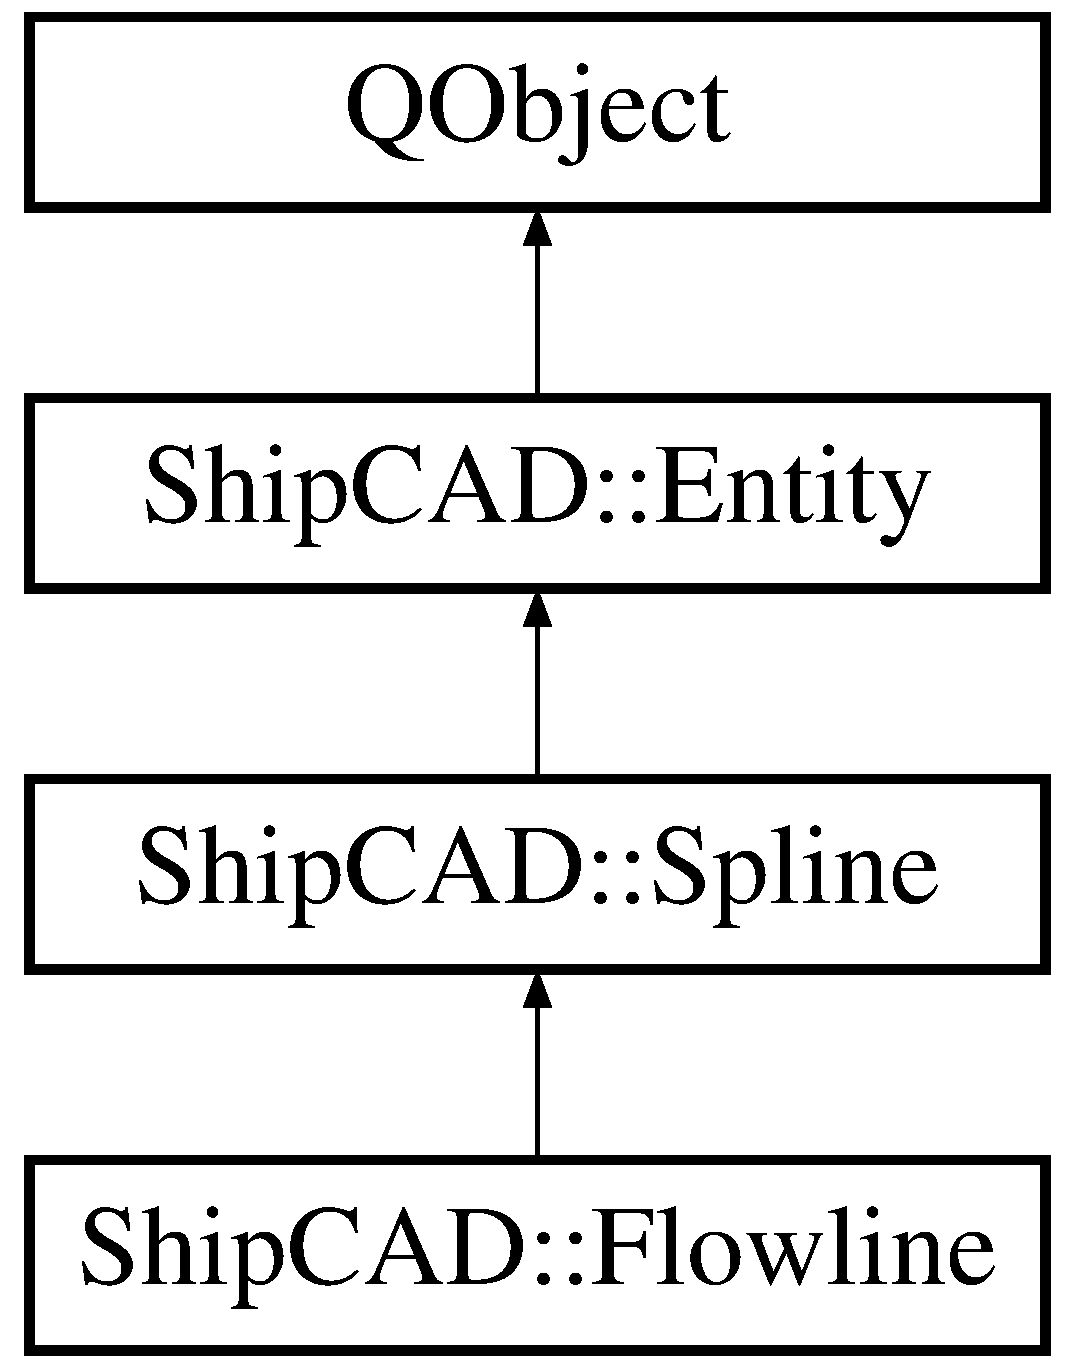
\includegraphics[height=4.000000cm]{classShipCAD_1_1Flowline}
\end{center}
\end{figure}
\subsection*{Public Member Functions}
\begin{DoxyCompactItemize}
\item 
\hyperlink{classShipCAD_1_1Flowline_aee316a748229f5abafac72ebe3af1e41}{Flowline} (\hyperlink{classShipCAD_1_1ShipCADModel}{Ship\+C\+A\+D\+Model} $\ast$owner)
\item 
virtual \hyperlink{classShipCAD_1_1Flowline_a77555e4dc8db9f99b684ea60e2a1a88e}{$\sim$\+Flowline} ()
\item 
void \hyperlink{classShipCAD_1_1Flowline_a58832002dec0b6ee8cb59e2fcc33f056}{initialize} (Q\+Vector2D pt, \hyperlink{namespaceShipCAD_aeeeb05810f2e31ef89fd4ac6b6ba9c0a}{viewport\+\_\+type\+\_\+t} ty)
\item 
virtual void \hyperlink{classShipCAD_1_1Flowline_ac3bbbbd3d853214bb9c9feeb7a12314d}{clear} ()
\item 
virtual void \hyperlink{classShipCAD_1_1Flowline_a8b43ac96514f62c6fb0db938eccd0d44}{draw} (\hyperlink{classShipCAD_1_1Viewport}{Viewport} \&vp, \hyperlink{classShipCAD_1_1LineShader}{Line\+Shader} $\ast$lineshader)
\item 
virtual void \hyperlink{classShipCAD_1_1Flowline_a28e5d73316c6d2c8005428669a9e9b97}{rebuild} ()
\item 
virtual void \hyperlink{classShipCAD_1_1Flowline_ad148400a3e53b2368b37c2c7f50ec1b7}{set\+Build} (bool val)
\item 
bool \hyperlink{classShipCAD_1_1Flowline_a86839bd40eccaef22050ba6f15aec361}{is\+Visible} () const 
\item 
bool \hyperlink{classShipCAD_1_1Flowline_a17a5a1693579fab85df64dac8f7a5fa8}{is\+Selected} () const 
\item 
void \hyperlink{classShipCAD_1_1Flowline_a4ade2663ee4102e0eff8920eeeaf8b37}{set\+Selected} (bool set)
\item 
virtual Q\+Color \hyperlink{classShipCAD_1_1Flowline_a546cee93d649cc3514bf2fcd19694ecf}{get\+Color} () const 
\item 
void \hyperlink{classShipCAD_1_1Flowline_a2910767b8fc3beb218d84bbb9d35fd7d}{load\+Binary} (\hyperlink{classShipCAD_1_1FileBuffer}{File\+Buffer} \&source)
\item 
void \hyperlink{classShipCAD_1_1Flowline_aeb29f59014b7df1e44dd6bda92dbc95d}{save\+Binary} (\hyperlink{classShipCAD_1_1FileBuffer}{File\+Buffer} \&dest)
\end{DoxyCompactItemize}
\subsection*{Static Public Member Functions}
\begin{DoxyCompactItemize}
\item 
static \hyperlink{classShipCAD_1_1Flowline}{Flowline} $\ast$ \hyperlink{classShipCAD_1_1Flowline_a9a07b50a90e9d96d347583dc15b5d07e}{construct} (\hyperlink{classShipCAD_1_1ShipCADModel}{Ship\+C\+A\+D\+Model} $\ast$owner)
\end{DoxyCompactItemize}
\subsection*{Additional Inherited Members}


\subsection{Detailed Description}


Definition at line 49 of file flowline.\+h.



\subsection{Constructor \& Destructor Documentation}
\index{Ship\+C\+A\+D\+::\+Flowline@{Ship\+C\+A\+D\+::\+Flowline}!Flowline@{Flowline}}
\index{Flowline@{Flowline}!Ship\+C\+A\+D\+::\+Flowline@{Ship\+C\+A\+D\+::\+Flowline}}
\subsubsection[{\texorpdfstring{Flowline(\+Ship\+C\+A\+D\+Model $\ast$owner)}{Flowline(ShipCADModel *owner)}}]{\setlength{\rightskip}{0pt plus 5cm}Flowline\+::\+Flowline (
\begin{DoxyParamCaption}
\item[{{\bf Ship\+C\+A\+D\+Model} $\ast$}]{owner}
\end{DoxyParamCaption}
)\hspace{0.3cm}{\ttfamily [explicit]}}\hypertarget{classShipCAD_1_1Flowline_aee316a748229f5abafac72ebe3af1e41}{}\label{classShipCAD_1_1Flowline_aee316a748229f5abafac72ebe3af1e41}


Definition at line 44 of file flowline.\+cpp.

\index{Ship\+C\+A\+D\+::\+Flowline@{Ship\+C\+A\+D\+::\+Flowline}!````~Flowline@{$\sim$\+Flowline}}
\index{````~Flowline@{$\sim$\+Flowline}!Ship\+C\+A\+D\+::\+Flowline@{Ship\+C\+A\+D\+::\+Flowline}}
\subsubsection[{\texorpdfstring{$\sim$\+Flowline()}{~Flowline()}}]{\setlength{\rightskip}{0pt plus 5cm}virtual Ship\+C\+A\+D\+::\+Flowline\+::$\sim$\+Flowline (
\begin{DoxyParamCaption}
{}
\end{DoxyParamCaption}
)\hspace{0.3cm}{\ttfamily [inline]}, {\ttfamily [virtual]}}\hypertarget{classShipCAD_1_1Flowline_a77555e4dc8db9f99b684ea60e2a1a88e}{}\label{classShipCAD_1_1Flowline_a77555e4dc8db9f99b684ea60e2a1a88e}


Definition at line 56 of file flowline.\+h.



\subsection{Member Function Documentation}
\index{Ship\+C\+A\+D\+::\+Flowline@{Ship\+C\+A\+D\+::\+Flowline}!clear@{clear}}
\index{clear@{clear}!Ship\+C\+A\+D\+::\+Flowline@{Ship\+C\+A\+D\+::\+Flowline}}
\subsubsection[{\texorpdfstring{clear()}{clear()}}]{\setlength{\rightskip}{0pt plus 5cm}void Flowline\+::clear (
\begin{DoxyParamCaption}
{}
\end{DoxyParamCaption}
)\hspace{0.3cm}{\ttfamily [virtual]}}\hypertarget{classShipCAD_1_1Flowline_ac3bbbbd3d853214bb9c9feeb7a12314d}{}\label{classShipCAD_1_1Flowline_ac3bbbbd3d853214bb9c9feeb7a12314d}


Reimplemented from \hyperlink{classShipCAD_1_1Spline_a02967f3eee8b1755eab0d7da55c3c621}{Ship\+C\+A\+D\+::\+Spline}.



Definition at line 56 of file flowline.\+cpp.

\index{Ship\+C\+A\+D\+::\+Flowline@{Ship\+C\+A\+D\+::\+Flowline}!construct@{construct}}
\index{construct@{construct}!Ship\+C\+A\+D\+::\+Flowline@{Ship\+C\+A\+D\+::\+Flowline}}
\subsubsection[{\texorpdfstring{construct(\+Ship\+C\+A\+D\+Model $\ast$owner)}{construct(ShipCADModel *owner)}}]{\setlength{\rightskip}{0pt plus 5cm}{\bf Flowline} $\ast$ Flowline\+::construct (
\begin{DoxyParamCaption}
\item[{{\bf Ship\+C\+A\+D\+Model} $\ast$}]{owner}
\end{DoxyParamCaption}
)\hspace{0.3cm}{\ttfamily [static]}}\hypertarget{classShipCAD_1_1Flowline_a9a07b50a90e9d96d347583dc15b5d07e}{}\label{classShipCAD_1_1Flowline_a9a07b50a90e9d96d347583dc15b5d07e}


Definition at line 50 of file flowline.\+cpp.

\index{Ship\+C\+A\+D\+::\+Flowline@{Ship\+C\+A\+D\+::\+Flowline}!draw@{draw}}
\index{draw@{draw}!Ship\+C\+A\+D\+::\+Flowline@{Ship\+C\+A\+D\+::\+Flowline}}
\subsubsection[{\texorpdfstring{draw(\+Viewport \&vp, Line\+Shader $\ast$lineshader)}{draw(Viewport &vp, LineShader *lineshader)}}]{\setlength{\rightskip}{0pt plus 5cm}void Flowline\+::draw (
\begin{DoxyParamCaption}
\item[{{\bf Viewport} \&}]{vp, }
\item[{{\bf Line\+Shader} $\ast$}]{lineshader}
\end{DoxyParamCaption}
)\hspace{0.3cm}{\ttfamily [virtual]}}\hypertarget{classShipCAD_1_1Flowline_a8b43ac96514f62c6fb0db938eccd0d44}{}\label{classShipCAD_1_1Flowline_a8b43ac96514f62c6fb0db938eccd0d44}


Reimplemented from \hyperlink{classShipCAD_1_1Spline_a6424ed433d241f566c15891cc25a74dd}{Ship\+C\+A\+D\+::\+Spline}.



Definition at line 72 of file flowline.\+cpp.

\index{Ship\+C\+A\+D\+::\+Flowline@{Ship\+C\+A\+D\+::\+Flowline}!get\+Color@{get\+Color}}
\index{get\+Color@{get\+Color}!Ship\+C\+A\+D\+::\+Flowline@{Ship\+C\+A\+D\+::\+Flowline}}
\subsubsection[{\texorpdfstring{get\+Color() const }{getColor() const }}]{\setlength{\rightskip}{0pt plus 5cm}Q\+Color Flowline\+::get\+Color (
\begin{DoxyParamCaption}
{}
\end{DoxyParamCaption}
) const\hspace{0.3cm}{\ttfamily [virtual]}}\hypertarget{classShipCAD_1_1Flowline_a546cee93d649cc3514bf2fcd19694ecf}{}\label{classShipCAD_1_1Flowline_a546cee93d649cc3514bf2fcd19694ecf}


Reimplemented from \hyperlink{classShipCAD_1_1Entity_a747f437fa410f5b8b6251967fd3a90aa}{Ship\+C\+A\+D\+::\+Entity}.



Definition at line 522 of file flowline.\+cpp.

\index{Ship\+C\+A\+D\+::\+Flowline@{Ship\+C\+A\+D\+::\+Flowline}!initialize@{initialize}}
\index{initialize@{initialize}!Ship\+C\+A\+D\+::\+Flowline@{Ship\+C\+A\+D\+::\+Flowline}}
\subsubsection[{\texorpdfstring{initialize(\+Q\+Vector2\+D pt, viewport\+\_\+type\+\_\+t ty)}{initialize(QVector2D pt, viewport_type_t ty)}}]{\setlength{\rightskip}{0pt plus 5cm}void Flowline\+::initialize (
\begin{DoxyParamCaption}
\item[{Q\+Vector2D}]{pt, }
\item[{{\bf viewport\+\_\+type\+\_\+t}}]{ty}
\end{DoxyParamCaption}
)}\hypertarget{classShipCAD_1_1Flowline_a58832002dec0b6ee8cb59e2fcc33f056}{}\label{classShipCAD_1_1Flowline_a58832002dec0b6ee8cb59e2fcc33f056}


Definition at line 64 of file flowline.\+cpp.

\index{Ship\+C\+A\+D\+::\+Flowline@{Ship\+C\+A\+D\+::\+Flowline}!is\+Selected@{is\+Selected}}
\index{is\+Selected@{is\+Selected}!Ship\+C\+A\+D\+::\+Flowline@{Ship\+C\+A\+D\+::\+Flowline}}
\subsubsection[{\texorpdfstring{is\+Selected() const }{isSelected() const }}]{\setlength{\rightskip}{0pt plus 5cm}bool Flowline\+::is\+Selected (
\begin{DoxyParamCaption}
{}
\end{DoxyParamCaption}
) const}\hypertarget{classShipCAD_1_1Flowline_a17a5a1693579fab85df64dac8f7a5fa8}{}\label{classShipCAD_1_1Flowline_a17a5a1693579fab85df64dac8f7a5fa8}


Definition at line 509 of file flowline.\+cpp.

\index{Ship\+C\+A\+D\+::\+Flowline@{Ship\+C\+A\+D\+::\+Flowline}!is\+Visible@{is\+Visible}}
\index{is\+Visible@{is\+Visible}!Ship\+C\+A\+D\+::\+Flowline@{Ship\+C\+A\+D\+::\+Flowline}}
\subsubsection[{\texorpdfstring{is\+Visible() const }{isVisible() const }}]{\setlength{\rightskip}{0pt plus 5cm}bool Flowline\+::is\+Visible (
\begin{DoxyParamCaption}
{}
\end{DoxyParamCaption}
) const}\hypertarget{classShipCAD_1_1Flowline_a86839bd40eccaef22050ba6f15aec361}{}\label{classShipCAD_1_1Flowline_a86839bd40eccaef22050ba6f15aec361}


Definition at line 504 of file flowline.\+cpp.

\index{Ship\+C\+A\+D\+::\+Flowline@{Ship\+C\+A\+D\+::\+Flowline}!load\+Binary@{load\+Binary}}
\index{load\+Binary@{load\+Binary}!Ship\+C\+A\+D\+::\+Flowline@{Ship\+C\+A\+D\+::\+Flowline}}
\subsubsection[{\texorpdfstring{load\+Binary(\+File\+Buffer \&source)}{loadBinary(FileBuffer &source)}}]{\setlength{\rightskip}{0pt plus 5cm}void Flowline\+::load\+Binary (
\begin{DoxyParamCaption}
\item[{{\bf File\+Buffer} \&}]{source}
\end{DoxyParamCaption}
)}\hypertarget{classShipCAD_1_1Flowline_a2910767b8fc3beb218d84bbb9d35fd7d}{}\label{classShipCAD_1_1Flowline_a2910767b8fc3beb218d84bbb9d35fd7d}


Definition at line 531 of file flowline.\+cpp.

\index{Ship\+C\+A\+D\+::\+Flowline@{Ship\+C\+A\+D\+::\+Flowline}!rebuild@{rebuild}}
\index{rebuild@{rebuild}!Ship\+C\+A\+D\+::\+Flowline@{Ship\+C\+A\+D\+::\+Flowline}}
\subsubsection[{\texorpdfstring{rebuild()}{rebuild()}}]{\setlength{\rightskip}{0pt plus 5cm}void Flowline\+::rebuild (
\begin{DoxyParamCaption}
{}
\end{DoxyParamCaption}
)\hspace{0.3cm}{\ttfamily [virtual]}}\hypertarget{classShipCAD_1_1Flowline_a28e5d73316c6d2c8005428669a9e9b97}{}\label{classShipCAD_1_1Flowline_a28e5d73316c6d2c8005428669a9e9b97}


Reimplemented from \hyperlink{classShipCAD_1_1Spline_a9b466ad7510032dafb0421f2d834bde6}{Ship\+C\+A\+D\+::\+Spline}.



Definition at line 364 of file flowline.\+cpp.

\index{Ship\+C\+A\+D\+::\+Flowline@{Ship\+C\+A\+D\+::\+Flowline}!save\+Binary@{save\+Binary}}
\index{save\+Binary@{save\+Binary}!Ship\+C\+A\+D\+::\+Flowline@{Ship\+C\+A\+D\+::\+Flowline}}
\subsubsection[{\texorpdfstring{save\+Binary(\+File\+Buffer \&dest)}{saveBinary(FileBuffer &dest)}}]{\setlength{\rightskip}{0pt plus 5cm}void Flowline\+::save\+Binary (
\begin{DoxyParamCaption}
\item[{{\bf File\+Buffer} \&}]{dest}
\end{DoxyParamCaption}
)}\hypertarget{classShipCAD_1_1Flowline_aeb29f59014b7df1e44dd6bda92dbc95d}{}\label{classShipCAD_1_1Flowline_aeb29f59014b7df1e44dd6bda92dbc95d}


Definition at line 556 of file flowline.\+cpp.

\index{Ship\+C\+A\+D\+::\+Flowline@{Ship\+C\+A\+D\+::\+Flowline}!set\+Build@{set\+Build}}
\index{set\+Build@{set\+Build}!Ship\+C\+A\+D\+::\+Flowline@{Ship\+C\+A\+D\+::\+Flowline}}
\subsubsection[{\texorpdfstring{set\+Build(bool val)}{setBuild(bool val)}}]{\setlength{\rightskip}{0pt plus 5cm}void Flowline\+::set\+Build (
\begin{DoxyParamCaption}
\item[{bool}]{val}
\end{DoxyParamCaption}
)\hspace{0.3cm}{\ttfamily [virtual]}}\hypertarget{classShipCAD_1_1Flowline_ad148400a3e53b2368b37c2c7f50ec1b7}{}\label{classShipCAD_1_1Flowline_ad148400a3e53b2368b37c2c7f50ec1b7}


Reimplemented from \hyperlink{classShipCAD_1_1Entity_a1889198398f42bb7f77a2334031c3f33}{Ship\+C\+A\+D\+::\+Entity}.



Definition at line 136 of file flowline.\+cpp.

\index{Ship\+C\+A\+D\+::\+Flowline@{Ship\+C\+A\+D\+::\+Flowline}!set\+Selected@{set\+Selected}}
\index{set\+Selected@{set\+Selected}!Ship\+C\+A\+D\+::\+Flowline@{Ship\+C\+A\+D\+::\+Flowline}}
\subsubsection[{\texorpdfstring{set\+Selected(bool set)}{setSelected(bool set)}}]{\setlength{\rightskip}{0pt plus 5cm}void Flowline\+::set\+Selected (
\begin{DoxyParamCaption}
\item[{bool}]{set}
\end{DoxyParamCaption}
)}\hypertarget{classShipCAD_1_1Flowline_a4ade2663ee4102e0eff8920eeeaf8b37}{}\label{classShipCAD_1_1Flowline_a4ade2663ee4102e0eff8920eeeaf8b37}


Definition at line 514 of file flowline.\+cpp.



The documentation for this class was generated from the following files\+:\begin{DoxyCompactItemize}
\item 
Ship\+C\+A\+Dlib/\hyperlink{flowline_8h}{flowline.\+h}\item 
Ship\+C\+A\+Dlib/\hyperlink{flowline_8cpp}{flowline.\+cpp}\end{DoxyCompactItemize}

\hypertarget{classShipCAD_1_1HydrostaticCalc}{}\section{Ship\+C\+AD\+:\+:Hydrostatic\+Calc Class Reference}
\label{classShipCAD_1_1HydrostaticCalc}\index{Ship\+C\+A\+D\+::\+Hydrostatic\+Calc@{Ship\+C\+A\+D\+::\+Hydrostatic\+Calc}}


Initialize and execute Hydrostatics Data calculation for a waterplane.  




{\ttfamily \#include $<$hydrostaticcalc.\+h$>$}

Inheritance diagram for Ship\+C\+AD\+:\+:Hydrostatic\+Calc\+:\begin{figure}[H]
\begin{center}
\leavevmode
\includegraphics[height=2.000000cm]{classShipCAD_1_1HydrostaticCalc}
\end{center}
\end{figure}
\subsection*{Public Member Functions}
\begin{DoxyCompactItemize}
\item 
\hyperlink{classShipCAD_1_1HydrostaticCalc_a56877acf4c33b3cab96ce381217c7a3b}{Hydrostatic\+Calc} (\hyperlink{classShipCAD_1_1ShipCADModel}{Ship\+C\+A\+D\+Model} $\ast$owner)
\item 
\hyperlink{classShipCAD_1_1HydrostaticCalc_a382835ae6396b82371b605d662fd1696}{$\sim$\+Hydrostatic\+Calc} ()
\item 
void \hyperlink{classShipCAD_1_1HydrostaticCalc_a09403d93ebe095a41b6a29ba9b740b65}{clear} ()
\item 
\hyperlink{classShipCAD_1_1ShipCADModel}{Ship\+C\+A\+D\+Model} $\ast$ \hyperlink{classShipCAD_1_1HydrostaticCalc_ac1dc0e446e711461bb3747326efd8df6}{get\+Owner} () const 
\item 
Q\+String \hyperlink{classShipCAD_1_1HydrostaticCalc_abfc3e3da906e630cf6b763bd3559c630}{get\+Error\+String} () const 
\begin{DoxyCompactList}\small\item\em get the errors with current calculation \end{DoxyCompactList}\item 
\hyperlink{classShipCAD_1_1Plane}{Plane} \hyperlink{classShipCAD_1_1HydrostaticCalc_a157563b0f0258d21a9be615e092d5b21}{get\+Wl\+Plane} () const 
\begin{DoxyCompactList}\small\item\em get the waterline plane (from draft, trim, and heeling angle) \end{DoxyCompactList}\item 
bool \hyperlink{classShipCAD_1_1HydrostaticCalc_a875b9708e91db4a8f06ddbcc8a22d830}{is\+Calculated} ()
\item 
void \hyperlink{classShipCAD_1_1HydrostaticCalc_a0deeafff07f3bb77184df959bbd91266}{set\+Calculated} (bool calc)
\item 
float \hyperlink{classShipCAD_1_1HydrostaticCalc_a3e1579cbcaddec517cfa95faa2228f2c}{get\+Draft} () const 
\item 
void \hyperlink{classShipCAD_1_1HydrostaticCalc_a6528fe532bbb1121c73972906d108835}{set\+Draft} (float draft)
\item 
\hyperlink{structShipCAD_1_1HydrostaticsData}{Hydrostatics\+Data} \& \hyperlink{classShipCAD_1_1HydrostaticCalc_aabcae04d59358b87b9d5fb4ffda83f1a}{get\+Data} ()
\item 
bool \hyperlink{classShipCAD_1_1HydrostaticCalc_a8ae6f41fd9799cb17a855a9b4f89c5fb}{has\+Error} (\hyperlink{namespaceShipCAD_a1d801b982c24bce0cf10ffd4b995dda0}{hydrostatics\+\_\+error\+\_\+t} error) const 
\begin{DoxyCompactList}\small\item\em does this calculation have this type of error \end{DoxyCompactList}\item 
void \hyperlink{classShipCAD_1_1HydrostaticCalc_ad6415cb7c8e13ded4537292dd3a06688}{add\+Error} (\hyperlink{namespaceShipCAD_a1d801b982c24bce0cf10ffd4b995dda0}{hydrostatics\+\_\+error\+\_\+t} error)
\begin{DoxyCompactList}\small\item\em add this error type to the calculation \end{DoxyCompactList}\item 
bool \hyperlink{classShipCAD_1_1HydrostaticCalc_adb8e8e29d28e2da0e75e30c0636f034b}{has\+Calculation} (\hyperlink{namespaceShipCAD_ac9ff7fc96a52fceafa83edc0d5d06fce}{hydrostatics\+\_\+calc\+\_\+t} ty) const 
\begin{DoxyCompactList}\small\item\em is this type of calculation set \end{DoxyCompactList}\item 
void \hyperlink{classShipCAD_1_1HydrostaticCalc_a32379831790fd88d422c6783b1b70ef7}{add\+Calculation\+Type} (\hyperlink{namespaceShipCAD_ac9ff7fc96a52fceafa83edc0d5d06fce}{hydrostatics\+\_\+calc\+\_\+t} ty)
\begin{DoxyCompactList}\small\item\em set a type of calculation \end{DoxyCompactList}\item 
float \hyperlink{classShipCAD_1_1HydrostaticCalc_a7b27fef68486f663fd325ef316032a03}{get\+Heeling\+Angle} () const 
\begin{DoxyCompactList}\small\item\em get the heeling angle for this calculation \end{DoxyCompactList}\item 
void \hyperlink{classShipCAD_1_1HydrostaticCalc_ae6bf118e2e5e89a8e8d7ea7675fdee22}{set\+Heeling\+Angle} (float angle)
\item 
void \hyperlink{classShipCAD_1_1HydrostaticCalc_a61df8d7421f2900cbc18a6565963c66e}{set\+Hydrostatic\+Type} (\hyperlink{namespaceShipCAD_afea51c7ee52940acebde29bf44206fe2}{hydrostatic\+\_\+type\+\_\+t} ty)
\item 
float \hyperlink{classShipCAD_1_1HydrostaticCalc_aecd19708f7ebadb4321af93565ffc184}{get\+Trim\+Angle} () const 
\begin{DoxyCompactList}\small\item\em get the trim angle for this calculation \end{DoxyCompactList}\item 
float \hyperlink{classShipCAD_1_1HydrostaticCalc_a90ae18aaf3a9836d01594cda165f35bb}{get\+Trim} () const 
\begin{DoxyCompactList}\small\item\em get the trim for this calculation (distance, not angle) \end{DoxyCompactList}\item 
void \hyperlink{classShipCAD_1_1HydrostaticCalc_ace579596fa77d8e3ea4f854ca033ed83}{set\+Trim} (float trim)
\begin{DoxyCompactList}\small\item\em set the trim for this calculation (distance, not angle) \end{DoxyCompactList}\item 
void \hyperlink{classShipCAD_1_1HydrostaticCalc_a919bce0b984cbef1c59534d6e9fec46f}{add\+Data} (Q\+String\+List \&strings, \hyperlink{namespaceShipCAD_a2c84d37615dd30be37ed0253501fb9a3}{hydrostatics\+\_\+mode\+\_\+t} mode, Q\+Char separator)
\begin{DoxyCompactList}\small\item\em get all Hydrostatics data in a list of strings \end{DoxyCompactList}\item 
bool \hyperlink{classShipCAD_1_1HydrostaticCalc_a7573a510a6b53e56a79f4042e41ee89e}{balance} (float displacement, bool freetotrim, \hyperlink{structShipCAD_1_1CrosscurvesData}{Crosscurves\+Data} \&output)
\item 
void \hyperlink{classShipCAD_1_1HydrostaticCalc_ab0c8f5dc5c576e6e9eae5fb27fd5bdd0}{calculate} ()
\begin{DoxyCompactList}\small\item\em make all calculations specified \end{DoxyCompactList}\item 
void \hyperlink{classShipCAD_1_1HydrostaticCalc_ad37fd32bf358c96b6653c6c92fd92c20}{calculate\+Volume} (const \hyperlink{classShipCAD_1_1Plane}{Plane} \&waterline\+\_\+plane)
\begin{DoxyCompactList}\small\item\em calculate the volume of the ship below plane \end{DoxyCompactList}\end{DoxyCompactItemize}
\subsection*{Static Public Member Functions}
\begin{DoxyCompactItemize}
\item 
static \hyperlink{classShipCAD_1_1HydrostaticCalc}{Hydrostatic\+Calc} $\ast$ \hyperlink{classShipCAD_1_1HydrostaticCalc_a527c0f0526a159e3d7cb7ddd4925c295}{construct} (\hyperlink{classShipCAD_1_1ShipCADModel}{Ship\+C\+A\+D\+Model} $\ast$owner)
\end{DoxyCompactItemize}
\subsection*{Protected Member Functions}
\begin{DoxyCompactItemize}
\item 
void \hyperlink{classShipCAD_1_1HydrostaticCalc_a95e0e1aa5d11f49cb0f0553ba45af085}{add\+Header} (Q\+String\+List \&strings)
\item 
void \hyperlink{classShipCAD_1_1HydrostaticCalc_aa4077ad7205ef509d3a54edb8e04b8b7}{add\+Footer} (Q\+String\+List \&strings, \hyperlink{namespaceShipCAD_a2c84d37615dd30be37ed0253501fb9a3}{hydrostatics\+\_\+mode\+\_\+t} mode)
\end{DoxyCompactItemize}


\subsection{Detailed Description}
Initialize and execute Hydrostatics Data calculation for a waterplane. 

Definition at line 106 of file hydrostaticcalc.\+h.



\subsection{Constructor \& Destructor Documentation}
\index{Ship\+C\+A\+D\+::\+Hydrostatic\+Calc@{Ship\+C\+A\+D\+::\+Hydrostatic\+Calc}!Hydrostatic\+Calc@{Hydrostatic\+Calc}}
\index{Hydrostatic\+Calc@{Hydrostatic\+Calc}!Ship\+C\+A\+D\+::\+Hydrostatic\+Calc@{Ship\+C\+A\+D\+::\+Hydrostatic\+Calc}}
\subsubsection[{\texorpdfstring{Hydrostatic\+Calc(\+Ship\+C\+A\+D\+Model $\ast$owner)}{HydrostaticCalc(ShipCADModel *owner)}}]{\setlength{\rightskip}{0pt plus 5cm}Hydrostatic\+Calc\+::\+Hydrostatic\+Calc (
\begin{DoxyParamCaption}
\item[{{\bf Ship\+C\+A\+D\+Model} $\ast$}]{owner}
\end{DoxyParamCaption}
)\hspace{0.3cm}{\ttfamily [explicit]}}\hypertarget{classShipCAD_1_1HydrostaticCalc_a56877acf4c33b3cab96ce381217c7a3b}{}\label{classShipCAD_1_1HydrostaticCalc_a56877acf4c33b3cab96ce381217c7a3b}


Definition at line 73 of file hydrostaticcalc.\+cpp.

\index{Ship\+C\+A\+D\+::\+Hydrostatic\+Calc@{Ship\+C\+A\+D\+::\+Hydrostatic\+Calc}!````~Hydrostatic\+Calc@{$\sim$\+Hydrostatic\+Calc}}
\index{````~Hydrostatic\+Calc@{$\sim$\+Hydrostatic\+Calc}!Ship\+C\+A\+D\+::\+Hydrostatic\+Calc@{Ship\+C\+A\+D\+::\+Hydrostatic\+Calc}}
\subsubsection[{\texorpdfstring{$\sim$\+Hydrostatic\+Calc()}{~HydrostaticCalc()}}]{\setlength{\rightskip}{0pt plus 5cm}Hydrostatic\+Calc\+::$\sim$\+Hydrostatic\+Calc (
\begin{DoxyParamCaption}
{}
\end{DoxyParamCaption}
)}\hypertarget{classShipCAD_1_1HydrostaticCalc_a382835ae6396b82371b605d662fd1696}{}\label{classShipCAD_1_1HydrostaticCalc_a382835ae6396b82371b605d662fd1696}


Definition at line 81 of file hydrostaticcalc.\+cpp.



\subsection{Member Function Documentation}
\index{Ship\+C\+A\+D\+::\+Hydrostatic\+Calc@{Ship\+C\+A\+D\+::\+Hydrostatic\+Calc}!add\+Calculation\+Type@{add\+Calculation\+Type}}
\index{add\+Calculation\+Type@{add\+Calculation\+Type}!Ship\+C\+A\+D\+::\+Hydrostatic\+Calc@{Ship\+C\+A\+D\+::\+Hydrostatic\+Calc}}
\subsubsection[{\texorpdfstring{add\+Calculation\+Type(hydrostatics\+\_\+calc\+\_\+t ty)}{addCalculationType(hydrostatics_calc_t ty)}}]{\setlength{\rightskip}{0pt plus 5cm}void Ship\+C\+A\+D\+::\+Hydrostatic\+Calc\+::add\+Calculation\+Type (
\begin{DoxyParamCaption}
\item[{{\bf hydrostatics\+\_\+calc\+\_\+t}}]{ty}
\end{DoxyParamCaption}
)\hspace{0.3cm}{\ttfamily [inline]}}\hypertarget{classShipCAD_1_1HydrostaticCalc_a32379831790fd88d422c6783b1b70ef7}{}\label{classShipCAD_1_1HydrostaticCalc_a32379831790fd88d422c6783b1b70ef7}


set a type of calculation 


\begin{DoxyParams}{Parameters}
{\em ty} & type of calculation to add to set \\
\hline
\end{DoxyParams}


Definition at line 156 of file hydrostaticcalc.\+h.

\index{Ship\+C\+A\+D\+::\+Hydrostatic\+Calc@{Ship\+C\+A\+D\+::\+Hydrostatic\+Calc}!add\+Data@{add\+Data}}
\index{add\+Data@{add\+Data}!Ship\+C\+A\+D\+::\+Hydrostatic\+Calc@{Ship\+C\+A\+D\+::\+Hydrostatic\+Calc}}
\subsubsection[{\texorpdfstring{add\+Data(\+Q\+String\+List \&strings, hydrostatics\+\_\+mode\+\_\+t mode, Q\+Char separator)}{addData(QStringList &strings, hydrostatics_mode_t mode, QChar separator)}}]{\setlength{\rightskip}{0pt plus 5cm}void Hydrostatic\+Calc\+::add\+Data (
\begin{DoxyParamCaption}
\item[{Q\+String\+List \&}]{strings, }
\item[{{\bf hydrostatics\+\_\+mode\+\_\+t}}]{mode, }
\item[{Q\+Char}]{separator}
\end{DoxyParamCaption}
)}\hypertarget{classShipCAD_1_1HydrostaticCalc_a919bce0b984cbef1c59534d6e9fec46f}{}\label{classShipCAD_1_1HydrostaticCalc_a919bce0b984cbef1c59534d6e9fec46f}


get all Hydrostatics data in a list of strings 


\begin{DoxyParams}{Parameters}
{\em strings} & target string list for data \\
\hline
{\em mode} & how to display the data \\
\hline
{\em separator} & character to separate the data \\
\hline
\end{DoxyParams}


Definition at line 189 of file hydrostaticcalc.\+cpp.

\index{Ship\+C\+A\+D\+::\+Hydrostatic\+Calc@{Ship\+C\+A\+D\+::\+Hydrostatic\+Calc}!add\+Error@{add\+Error}}
\index{add\+Error@{add\+Error}!Ship\+C\+A\+D\+::\+Hydrostatic\+Calc@{Ship\+C\+A\+D\+::\+Hydrostatic\+Calc}}
\subsubsection[{\texorpdfstring{add\+Error(hydrostatics\+\_\+error\+\_\+t error)}{addError(hydrostatics_error_t error)}}]{\setlength{\rightskip}{0pt plus 5cm}void Ship\+C\+A\+D\+::\+Hydrostatic\+Calc\+::add\+Error (
\begin{DoxyParamCaption}
\item[{{\bf hydrostatics\+\_\+error\+\_\+t}}]{error}
\end{DoxyParamCaption}
)\hspace{0.3cm}{\ttfamily [inline]}}\hypertarget{classShipCAD_1_1HydrostaticCalc_ad6415cb7c8e13ded4537292dd3a06688}{}\label{classShipCAD_1_1HydrostaticCalc_ad6415cb7c8e13ded4537292dd3a06688}


add this error type to the calculation 


\begin{DoxyParams}{Parameters}
{\em error} & the error to add \\
\hline
\end{DoxyParams}


Definition at line 145 of file hydrostaticcalc.\+h.

\index{Ship\+C\+A\+D\+::\+Hydrostatic\+Calc@{Ship\+C\+A\+D\+::\+Hydrostatic\+Calc}!add\+Footer@{add\+Footer}}
\index{add\+Footer@{add\+Footer}!Ship\+C\+A\+D\+::\+Hydrostatic\+Calc@{Ship\+C\+A\+D\+::\+Hydrostatic\+Calc}}
\subsubsection[{\texorpdfstring{add\+Footer(\+Q\+String\+List \&strings, hydrostatics\+\_\+mode\+\_\+t mode)}{addFooter(QStringList &strings, hydrostatics_mode_t mode)}}]{\setlength{\rightskip}{0pt plus 5cm}void Hydrostatic\+Calc\+::add\+Footer (
\begin{DoxyParamCaption}
\item[{Q\+String\+List \&}]{strings, }
\item[{{\bf hydrostatics\+\_\+mode\+\_\+t}}]{mode}
\end{DoxyParamCaption}
)\hspace{0.3cm}{\ttfamily [protected]}}\hypertarget{classShipCAD_1_1HydrostaticCalc_aa4077ad7205ef509d3a54edb8e04b8b7}{}\label{classShipCAD_1_1HydrostaticCalc_aa4077ad7205ef509d3a54edb8e04b8b7}


Definition at line 391 of file hydrostaticcalc.\+cpp.

\index{Ship\+C\+A\+D\+::\+Hydrostatic\+Calc@{Ship\+C\+A\+D\+::\+Hydrostatic\+Calc}!add\+Header@{add\+Header}}
\index{add\+Header@{add\+Header}!Ship\+C\+A\+D\+::\+Hydrostatic\+Calc@{Ship\+C\+A\+D\+::\+Hydrostatic\+Calc}}
\subsubsection[{\texorpdfstring{add\+Header(\+Q\+String\+List \&strings)}{addHeader(QStringList &strings)}}]{\setlength{\rightskip}{0pt plus 5cm}void Hydrostatic\+Calc\+::add\+Header (
\begin{DoxyParamCaption}
\item[{Q\+String\+List \&}]{strings}
\end{DoxyParamCaption}
)\hspace{0.3cm}{\ttfamily [protected]}}\hypertarget{classShipCAD_1_1HydrostaticCalc_a95e0e1aa5d11f49cb0f0553ba45af085}{}\label{classShipCAD_1_1HydrostaticCalc_a95e0e1aa5d11f49cb0f0553ba45af085}


Definition at line 350 of file hydrostaticcalc.\+cpp.

\index{Ship\+C\+A\+D\+::\+Hydrostatic\+Calc@{Ship\+C\+A\+D\+::\+Hydrostatic\+Calc}!balance@{balance}}
\index{balance@{balance}!Ship\+C\+A\+D\+::\+Hydrostatic\+Calc@{Ship\+C\+A\+D\+::\+Hydrostatic\+Calc}}
\subsubsection[{\texorpdfstring{balance(float displacement, bool freetotrim, Crosscurves\+Data \&output)}{balance(float displacement, bool freetotrim, CrosscurvesData &output)}}]{\setlength{\rightskip}{0pt plus 5cm}bool Hydrostatic\+Calc\+::balance (
\begin{DoxyParamCaption}
\item[{float}]{displacement, }
\item[{bool}]{freetotrim, }
\item[{{\bf Crosscurves\+Data} \&}]{output}
\end{DoxyParamCaption}
)}\hypertarget{classShipCAD_1_1HydrostaticCalc_a7573a510a6b53e56a79f4042e41ee89e}{}\label{classShipCAD_1_1HydrostaticCalc_a7573a510a6b53e56a79f4042e41ee89e}


Definition at line 579 of file hydrostaticcalc.\+cpp.

\index{Ship\+C\+A\+D\+::\+Hydrostatic\+Calc@{Ship\+C\+A\+D\+::\+Hydrostatic\+Calc}!calculate@{calculate}}
\index{calculate@{calculate}!Ship\+C\+A\+D\+::\+Hydrostatic\+Calc@{Ship\+C\+A\+D\+::\+Hydrostatic\+Calc}}
\subsubsection[{\texorpdfstring{calculate()}{calculate()}}]{\setlength{\rightskip}{0pt plus 5cm}void Hydrostatic\+Calc\+::calculate (
\begin{DoxyParamCaption}
{}
\end{DoxyParamCaption}
)}\hypertarget{classShipCAD_1_1HydrostaticCalc_ab0c8f5dc5c576e6e9eae5fb27fd5bdd0}{}\label{classShipCAD_1_1HydrostaticCalc_ab0c8f5dc5c576e6e9eae5fb27fd5bdd0}


make all calculations specified 

For each type of calculation specified, this method will fill out \+\_\+data with the results of that calculation The calculated flag will also be set 

Definition at line 920 of file hydrostaticcalc.\+cpp.

\index{Ship\+C\+A\+D\+::\+Hydrostatic\+Calc@{Ship\+C\+A\+D\+::\+Hydrostatic\+Calc}!calculate\+Volume@{calculate\+Volume}}
\index{calculate\+Volume@{calculate\+Volume}!Ship\+C\+A\+D\+::\+Hydrostatic\+Calc@{Ship\+C\+A\+D\+::\+Hydrostatic\+Calc}}
\subsubsection[{\texorpdfstring{calculate\+Volume(const Plane \&waterline\+\_\+plane)}{calculateVolume(const Plane &waterline_plane)}}]{\setlength{\rightskip}{0pt plus 5cm}void Hydrostatic\+Calc\+::calculate\+Volume (
\begin{DoxyParamCaption}
\item[{const {\bf Plane} \&}]{waterline\+\_\+plane}
\end{DoxyParamCaption}
)}\hypertarget{classShipCAD_1_1HydrostaticCalc_ad37fd32bf358c96b6653c6c92fd92c20}{}\label{classShipCAD_1_1HydrostaticCalc_ad37fd32bf358c96b6653c6c92fd92c20}


calculate the volume of the ship below plane 

When this method is completed, then \+\_\+data will have absolute\+\_\+draft, errors, leak point, center\+\_\+of\+\_\+buoyancy, lcb\+\_\+perc, length\+\_\+waterline, width\+\_\+waterline, displacement, volume calculated The calculated flag will also be set


\begin{DoxyParams}{Parameters}
{\em waterline\+\_\+plane} & the plane of the waterline \\
\hline
\end{DoxyParams}


Definition at line 1058 of file hydrostaticcalc.\+cpp.

\index{Ship\+C\+A\+D\+::\+Hydrostatic\+Calc@{Ship\+C\+A\+D\+::\+Hydrostatic\+Calc}!clear@{clear}}
\index{clear@{clear}!Ship\+C\+A\+D\+::\+Hydrostatic\+Calc@{Ship\+C\+A\+D\+::\+Hydrostatic\+Calc}}
\subsubsection[{\texorpdfstring{clear()}{clear()}}]{\setlength{\rightskip}{0pt plus 5cm}void Hydrostatic\+Calc\+::clear (
\begin{DoxyParamCaption}
{}
\end{DoxyParamCaption}
)}\hypertarget{classShipCAD_1_1HydrostaticCalc_a09403d93ebe095a41b6a29ba9b740b65}{}\label{classShipCAD_1_1HydrostaticCalc_a09403d93ebe095a41b6a29ba9b740b65}


Definition at line 92 of file hydrostaticcalc.\+cpp.

\index{Ship\+C\+A\+D\+::\+Hydrostatic\+Calc@{Ship\+C\+A\+D\+::\+Hydrostatic\+Calc}!construct@{construct}}
\index{construct@{construct}!Ship\+C\+A\+D\+::\+Hydrostatic\+Calc@{Ship\+C\+A\+D\+::\+Hydrostatic\+Calc}}
\subsubsection[{\texorpdfstring{construct(\+Ship\+C\+A\+D\+Model $\ast$owner)}{construct(ShipCADModel *owner)}}]{\setlength{\rightskip}{0pt plus 5cm}{\bf Hydrostatic\+Calc} $\ast$ Hydrostatic\+Calc\+::construct (
\begin{DoxyParamCaption}
\item[{{\bf Ship\+C\+A\+D\+Model} $\ast$}]{owner}
\end{DoxyParamCaption}
)\hspace{0.3cm}{\ttfamily [static]}}\hypertarget{classShipCAD_1_1HydrostaticCalc_a527c0f0526a159e3d7cb7ddd4925c295}{}\label{classShipCAD_1_1HydrostaticCalc_a527c0f0526a159e3d7cb7ddd4925c295}


Definition at line 86 of file hydrostaticcalc.\+cpp.

\index{Ship\+C\+A\+D\+::\+Hydrostatic\+Calc@{Ship\+C\+A\+D\+::\+Hydrostatic\+Calc}!get\+Data@{get\+Data}}
\index{get\+Data@{get\+Data}!Ship\+C\+A\+D\+::\+Hydrostatic\+Calc@{Ship\+C\+A\+D\+::\+Hydrostatic\+Calc}}
\subsubsection[{\texorpdfstring{get\+Data()}{getData()}}]{\setlength{\rightskip}{0pt plus 5cm}{\bf Hydrostatics\+Data}\& Ship\+C\+A\+D\+::\+Hydrostatic\+Calc\+::get\+Data (
\begin{DoxyParamCaption}
{}
\end{DoxyParamCaption}
)\hspace{0.3cm}{\ttfamily [inline]}}\hypertarget{classShipCAD_1_1HydrostaticCalc_aabcae04d59358b87b9d5fb4ffda83f1a}{}\label{classShipCAD_1_1HydrostaticCalc_aabcae04d59358b87b9d5fb4ffda83f1a}


Definition at line 134 of file hydrostaticcalc.\+h.

\index{Ship\+C\+A\+D\+::\+Hydrostatic\+Calc@{Ship\+C\+A\+D\+::\+Hydrostatic\+Calc}!get\+Draft@{get\+Draft}}
\index{get\+Draft@{get\+Draft}!Ship\+C\+A\+D\+::\+Hydrostatic\+Calc@{Ship\+C\+A\+D\+::\+Hydrostatic\+Calc}}
\subsubsection[{\texorpdfstring{get\+Draft() const }{getDraft() const }}]{\setlength{\rightskip}{0pt plus 5cm}float Ship\+C\+A\+D\+::\+Hydrostatic\+Calc\+::get\+Draft (
\begin{DoxyParamCaption}
{}
\end{DoxyParamCaption}
) const\hspace{0.3cm}{\ttfamily [inline]}}\hypertarget{classShipCAD_1_1HydrostaticCalc_a3e1579cbcaddec517cfa95faa2228f2c}{}\label{classShipCAD_1_1HydrostaticCalc_a3e1579cbcaddec517cfa95faa2228f2c}


Definition at line 132 of file hydrostaticcalc.\+h.

\index{Ship\+C\+A\+D\+::\+Hydrostatic\+Calc@{Ship\+C\+A\+D\+::\+Hydrostatic\+Calc}!get\+Error\+String@{get\+Error\+String}}
\index{get\+Error\+String@{get\+Error\+String}!Ship\+C\+A\+D\+::\+Hydrostatic\+Calc@{Ship\+C\+A\+D\+::\+Hydrostatic\+Calc}}
\subsubsection[{\texorpdfstring{get\+Error\+String() const }{getErrorString() const }}]{\setlength{\rightskip}{0pt plus 5cm}Q\+String Hydrostatic\+Calc\+::get\+Error\+String (
\begin{DoxyParamCaption}
{}
\end{DoxyParamCaption}
) const}\hypertarget{classShipCAD_1_1HydrostaticCalc_abfc3e3da906e630cf6b763bd3559c630}{}\label{classShipCAD_1_1HydrostaticCalc_abfc3e3da906e630cf6b763bd3559c630}


get the errors with current calculation 

\begin{DoxyReturn}{Returns}
string with current errors 
\end{DoxyReturn}


Definition at line 104 of file hydrostaticcalc.\+cpp.

\index{Ship\+C\+A\+D\+::\+Hydrostatic\+Calc@{Ship\+C\+A\+D\+::\+Hydrostatic\+Calc}!get\+Heeling\+Angle@{get\+Heeling\+Angle}}
\index{get\+Heeling\+Angle@{get\+Heeling\+Angle}!Ship\+C\+A\+D\+::\+Hydrostatic\+Calc@{Ship\+C\+A\+D\+::\+Hydrostatic\+Calc}}
\subsubsection[{\texorpdfstring{get\+Heeling\+Angle() const }{getHeelingAngle() const }}]{\setlength{\rightskip}{0pt plus 5cm}float Ship\+C\+A\+D\+::\+Hydrostatic\+Calc\+::get\+Heeling\+Angle (
\begin{DoxyParamCaption}
{}
\end{DoxyParamCaption}
) const\hspace{0.3cm}{\ttfamily [inline]}}\hypertarget{classShipCAD_1_1HydrostaticCalc_a7b27fef68486f663fd325ef316032a03}{}\label{classShipCAD_1_1HydrostaticCalc_a7b27fef68486f663fd325ef316032a03}


get the heeling angle for this calculation 

\begin{DoxyReturn}{Returns}
the heeling angle in degrees 
\end{DoxyReturn}


Definition at line 162 of file hydrostaticcalc.\+h.

\index{Ship\+C\+A\+D\+::\+Hydrostatic\+Calc@{Ship\+C\+A\+D\+::\+Hydrostatic\+Calc}!get\+Owner@{get\+Owner}}
\index{get\+Owner@{get\+Owner}!Ship\+C\+A\+D\+::\+Hydrostatic\+Calc@{Ship\+C\+A\+D\+::\+Hydrostatic\+Calc}}
\subsubsection[{\texorpdfstring{get\+Owner() const }{getOwner() const }}]{\setlength{\rightskip}{0pt plus 5cm}{\bf Ship\+C\+A\+D\+Model}$\ast$ Ship\+C\+A\+D\+::\+Hydrostatic\+Calc\+::get\+Owner (
\begin{DoxyParamCaption}
{}
\end{DoxyParamCaption}
) const\hspace{0.3cm}{\ttfamily [inline]}}\hypertarget{classShipCAD_1_1HydrostaticCalc_ac1dc0e446e711461bb3747326efd8df6}{}\label{classShipCAD_1_1HydrostaticCalc_ac1dc0e446e711461bb3747326efd8df6}


Definition at line 118 of file hydrostaticcalc.\+h.

\index{Ship\+C\+A\+D\+::\+Hydrostatic\+Calc@{Ship\+C\+A\+D\+::\+Hydrostatic\+Calc}!get\+Trim@{get\+Trim}}
\index{get\+Trim@{get\+Trim}!Ship\+C\+A\+D\+::\+Hydrostatic\+Calc@{Ship\+C\+A\+D\+::\+Hydrostatic\+Calc}}
\subsubsection[{\texorpdfstring{get\+Trim() const }{getTrim() const }}]{\setlength{\rightskip}{0pt plus 5cm}float Ship\+C\+A\+D\+::\+Hydrostatic\+Calc\+::get\+Trim (
\begin{DoxyParamCaption}
{}
\end{DoxyParamCaption}
) const\hspace{0.3cm}{\ttfamily [inline]}}\hypertarget{classShipCAD_1_1HydrostaticCalc_a90ae18aaf3a9836d01594cda165f35bb}{}\label{classShipCAD_1_1HydrostaticCalc_a90ae18aaf3a9836d01594cda165f35bb}


get the trim for this calculation (distance, not angle) 

\begin{DoxyReturn}{Returns}
the trim 
\end{DoxyReturn}


Definition at line 178 of file hydrostaticcalc.\+h.

\index{Ship\+C\+A\+D\+::\+Hydrostatic\+Calc@{Ship\+C\+A\+D\+::\+Hydrostatic\+Calc}!get\+Trim\+Angle@{get\+Trim\+Angle}}
\index{get\+Trim\+Angle@{get\+Trim\+Angle}!Ship\+C\+A\+D\+::\+Hydrostatic\+Calc@{Ship\+C\+A\+D\+::\+Hydrostatic\+Calc}}
\subsubsection[{\texorpdfstring{get\+Trim\+Angle() const }{getTrimAngle() const }}]{\setlength{\rightskip}{0pt plus 5cm}float Hydrostatic\+Calc\+::get\+Trim\+Angle (
\begin{DoxyParamCaption}
{}
\end{DoxyParamCaption}
) const}\hypertarget{classShipCAD_1_1HydrostaticCalc_aecd19708f7ebadb4321af93565ffc184}{}\label{classShipCAD_1_1HydrostaticCalc_aecd19708f7ebadb4321af93565ffc184}


get the trim angle for this calculation 

The trim angle is calculated from the given trim and waterline plane.

\begin{DoxyReturn}{Returns}
the angle of trim in degrees 
\end{DoxyReturn}


Definition at line 118 of file hydrostaticcalc.\+cpp.

\index{Ship\+C\+A\+D\+::\+Hydrostatic\+Calc@{Ship\+C\+A\+D\+::\+Hydrostatic\+Calc}!get\+Wl\+Plane@{get\+Wl\+Plane}}
\index{get\+Wl\+Plane@{get\+Wl\+Plane}!Ship\+C\+A\+D\+::\+Hydrostatic\+Calc@{Ship\+C\+A\+D\+::\+Hydrostatic\+Calc}}
\subsubsection[{\texorpdfstring{get\+Wl\+Plane() const }{getWlPlane() const }}]{\setlength{\rightskip}{0pt plus 5cm}{\bf Plane} Hydrostatic\+Calc\+::get\+Wl\+Plane (
\begin{DoxyParamCaption}
{}
\end{DoxyParamCaption}
) const}\hypertarget{classShipCAD_1_1HydrostaticCalc_a157563b0f0258d21a9be615e092d5b21}{}\label{classShipCAD_1_1HydrostaticCalc_a157563b0f0258d21a9be615e092d5b21}


get the waterline plane (from draft, trim, and heeling angle) 

\begin{DoxyReturn}{Returns}
the waterline plane 
\end{DoxyReturn}


Definition at line 125 of file hydrostaticcalc.\+cpp.

\index{Ship\+C\+A\+D\+::\+Hydrostatic\+Calc@{Ship\+C\+A\+D\+::\+Hydrostatic\+Calc}!has\+Calculation@{has\+Calculation}}
\index{has\+Calculation@{has\+Calculation}!Ship\+C\+A\+D\+::\+Hydrostatic\+Calc@{Ship\+C\+A\+D\+::\+Hydrostatic\+Calc}}
\subsubsection[{\texorpdfstring{has\+Calculation(hydrostatics\+\_\+calc\+\_\+t ty) const }{hasCalculation(hydrostatics_calc_t ty) const }}]{\setlength{\rightskip}{0pt plus 5cm}bool Hydrostatic\+Calc\+::has\+Calculation (
\begin{DoxyParamCaption}
\item[{{\bf hydrostatics\+\_\+calc\+\_\+t}}]{ty}
\end{DoxyParamCaption}
) const}\hypertarget{classShipCAD_1_1HydrostaticCalc_adb8e8e29d28e2da0e75e30c0636f034b}{}\label{classShipCAD_1_1HydrostaticCalc_adb8e8e29d28e2da0e75e30c0636f034b}


is this type of calculation set 


\begin{DoxyParams}{Parameters}
{\em ty} & type of calculation to check for \\
\hline
\end{DoxyParams}
\begin{DoxyReturn}{Returns}
true if type is part of set 
\end{DoxyReturn}


Definition at line 184 of file hydrostaticcalc.\+cpp.

\index{Ship\+C\+A\+D\+::\+Hydrostatic\+Calc@{Ship\+C\+A\+D\+::\+Hydrostatic\+Calc}!has\+Error@{has\+Error}}
\index{has\+Error@{has\+Error}!Ship\+C\+A\+D\+::\+Hydrostatic\+Calc@{Ship\+C\+A\+D\+::\+Hydrostatic\+Calc}}
\subsubsection[{\texorpdfstring{has\+Error(hydrostatics\+\_\+error\+\_\+t error) const }{hasError(hydrostatics_error_t error) const }}]{\setlength{\rightskip}{0pt plus 5cm}bool Hydrostatic\+Calc\+::has\+Error (
\begin{DoxyParamCaption}
\item[{{\bf hydrostatics\+\_\+error\+\_\+t}}]{error}
\end{DoxyParamCaption}
) const}\hypertarget{classShipCAD_1_1HydrostaticCalc_a8ae6f41fd9799cb17a855a9b4f89c5fb}{}\label{classShipCAD_1_1HydrostaticCalc_a8ae6f41fd9799cb17a855a9b4f89c5fb}


does this calculation have this type of error 


\begin{DoxyParams}{Parameters}
{\em error} & the error to check for \\
\hline
\end{DoxyParams}
\begin{DoxyReturn}{Returns}
true if calculation has this error 
\end{DoxyReturn}


Definition at line 179 of file hydrostaticcalc.\+cpp.

\index{Ship\+C\+A\+D\+::\+Hydrostatic\+Calc@{Ship\+C\+A\+D\+::\+Hydrostatic\+Calc}!is\+Calculated@{is\+Calculated}}
\index{is\+Calculated@{is\+Calculated}!Ship\+C\+A\+D\+::\+Hydrostatic\+Calc@{Ship\+C\+A\+D\+::\+Hydrostatic\+Calc}}
\subsubsection[{\texorpdfstring{is\+Calculated()}{isCalculated()}}]{\setlength{\rightskip}{0pt plus 5cm}bool Ship\+C\+A\+D\+::\+Hydrostatic\+Calc\+::is\+Calculated (
\begin{DoxyParamCaption}
{}
\end{DoxyParamCaption}
)\hspace{0.3cm}{\ttfamily [inline]}}\hypertarget{classShipCAD_1_1HydrostaticCalc_a875b9708e91db4a8f06ddbcc8a22d830}{}\label{classShipCAD_1_1HydrostaticCalc_a875b9708e91db4a8f06ddbcc8a22d830}


Definition at line 130 of file hydrostaticcalc.\+h.

\index{Ship\+C\+A\+D\+::\+Hydrostatic\+Calc@{Ship\+C\+A\+D\+::\+Hydrostatic\+Calc}!set\+Calculated@{set\+Calculated}}
\index{set\+Calculated@{set\+Calculated}!Ship\+C\+A\+D\+::\+Hydrostatic\+Calc@{Ship\+C\+A\+D\+::\+Hydrostatic\+Calc}}
\subsubsection[{\texorpdfstring{set\+Calculated(bool calc)}{setCalculated(bool calc)}}]{\setlength{\rightskip}{0pt plus 5cm}void Hydrostatic\+Calc\+::set\+Calculated (
\begin{DoxyParamCaption}
\item[{bool}]{calc}
\end{DoxyParamCaption}
)}\hypertarget{classShipCAD_1_1HydrostaticCalc_a0deeafff07f3bb77184df959bbd91266}{}\label{classShipCAD_1_1HydrostaticCalc_a0deeafff07f3bb77184df959bbd91266}


Definition at line 137 of file hydrostaticcalc.\+cpp.

\index{Ship\+C\+A\+D\+::\+Hydrostatic\+Calc@{Ship\+C\+A\+D\+::\+Hydrostatic\+Calc}!set\+Draft@{set\+Draft}}
\index{set\+Draft@{set\+Draft}!Ship\+C\+A\+D\+::\+Hydrostatic\+Calc@{Ship\+C\+A\+D\+::\+Hydrostatic\+Calc}}
\subsubsection[{\texorpdfstring{set\+Draft(float draft)}{setDraft(float draft)}}]{\setlength{\rightskip}{0pt plus 5cm}void Hydrostatic\+Calc\+::set\+Draft (
\begin{DoxyParamCaption}
\item[{float}]{draft}
\end{DoxyParamCaption}
)}\hypertarget{classShipCAD_1_1HydrostaticCalc_a6528fe532bbb1121c73972906d108835}{}\label{classShipCAD_1_1HydrostaticCalc_a6528fe532bbb1121c73972906d108835}


Definition at line 147 of file hydrostaticcalc.\+cpp.

\index{Ship\+C\+A\+D\+::\+Hydrostatic\+Calc@{Ship\+C\+A\+D\+::\+Hydrostatic\+Calc}!set\+Heeling\+Angle@{set\+Heeling\+Angle}}
\index{set\+Heeling\+Angle@{set\+Heeling\+Angle}!Ship\+C\+A\+D\+::\+Hydrostatic\+Calc@{Ship\+C\+A\+D\+::\+Hydrostatic\+Calc}}
\subsubsection[{\texorpdfstring{set\+Heeling\+Angle(float angle)}{setHeelingAngle(float angle)}}]{\setlength{\rightskip}{0pt plus 5cm}void Hydrostatic\+Calc\+::set\+Heeling\+Angle (
\begin{DoxyParamCaption}
\item[{float}]{angle}
\end{DoxyParamCaption}
)}\hypertarget{classShipCAD_1_1HydrostaticCalc_ae6bf118e2e5e89a8e8d7ea7675fdee22}{}\label{classShipCAD_1_1HydrostaticCalc_ae6bf118e2e5e89a8e8d7ea7675fdee22}


Definition at line 155 of file hydrostaticcalc.\+cpp.

\index{Ship\+C\+A\+D\+::\+Hydrostatic\+Calc@{Ship\+C\+A\+D\+::\+Hydrostatic\+Calc}!set\+Hydrostatic\+Type@{set\+Hydrostatic\+Type}}
\index{set\+Hydrostatic\+Type@{set\+Hydrostatic\+Type}!Ship\+C\+A\+D\+::\+Hydrostatic\+Calc@{Ship\+C\+A\+D\+::\+Hydrostatic\+Calc}}
\subsubsection[{\texorpdfstring{set\+Hydrostatic\+Type(hydrostatic\+\_\+type\+\_\+t ty)}{setHydrostaticType(hydrostatic_type_t ty)}}]{\setlength{\rightskip}{0pt plus 5cm}void Hydrostatic\+Calc\+::set\+Hydrostatic\+Type (
\begin{DoxyParamCaption}
\item[{{\bf hydrostatic\+\_\+type\+\_\+t}}]{ty}
\end{DoxyParamCaption}
)}\hypertarget{classShipCAD_1_1HydrostaticCalc_a61df8d7421f2900cbc18a6565963c66e}{}\label{classShipCAD_1_1HydrostaticCalc_a61df8d7421f2900cbc18a6565963c66e}


Definition at line 163 of file hydrostaticcalc.\+cpp.

\index{Ship\+C\+A\+D\+::\+Hydrostatic\+Calc@{Ship\+C\+A\+D\+::\+Hydrostatic\+Calc}!set\+Trim@{set\+Trim}}
\index{set\+Trim@{set\+Trim}!Ship\+C\+A\+D\+::\+Hydrostatic\+Calc@{Ship\+C\+A\+D\+::\+Hydrostatic\+Calc}}
\subsubsection[{\texorpdfstring{set\+Trim(float trim)}{setTrim(float trim)}}]{\setlength{\rightskip}{0pt plus 5cm}void Hydrostatic\+Calc\+::set\+Trim (
\begin{DoxyParamCaption}
\item[{float}]{trim}
\end{DoxyParamCaption}
)}\hypertarget{classShipCAD_1_1HydrostaticCalc_ace579596fa77d8e3ea4f854ca033ed83}{}\label{classShipCAD_1_1HydrostaticCalc_ace579596fa77d8e3ea4f854ca033ed83}


set the trim for this calculation (distance, not angle) 


\begin{DoxyParams}{Parameters}
{\em trim} & the trim of the hull \\
\hline
\end{DoxyParams}


Definition at line 171 of file hydrostaticcalc.\+cpp.



The documentation for this class was generated from the following files\+:\begin{DoxyCompactItemize}
\item 
Ship\+C\+A\+Dlib/\hyperlink{hydrostaticcalc_8h}{hydrostaticcalc.\+h}\item 
Ship\+C\+A\+Dlib/\hyperlink{hydrostaticcalc_8cpp}{hydrostaticcalc.\+cpp}\end{DoxyCompactItemize}

\hypertarget{structShipCAD_1_1HydrostaticsData}{}\section{Ship\+C\+AD\+:\+:Hydrostatics\+Data Struct Reference}
\label{structShipCAD_1_1HydrostaticsData}\index{Ship\+C\+A\+D\+::\+Hydrostatics\+Data@{Ship\+C\+A\+D\+::\+Hydrostatics\+Data}}


Hydrostatics Calculation results.  




{\ttfamily \#include $<$hydrostaticcalc.\+h$>$}

\subsection*{Public Member Functions}
\begin{DoxyCompactItemize}
\item 
void \hyperlink{structShipCAD_1_1HydrostaticsData_a7ea81ac589a3b24424b4176c734c7a37}{clear} ()
\begin{DoxyCompactList}\small\item\em reset all data to default values \end{DoxyCompactList}\end{DoxyCompactItemize}
\subsection*{Public Attributes}
\begin{DoxyCompactItemize}
\item 
Q\+Vector3D \hyperlink{structShipCAD_1_1HydrostaticsData_acd93669bc08fa097974d41fbaf4dc81f}{model\+\_\+min}
\item 
Q\+Vector3D \hyperlink{structShipCAD_1_1HydrostaticsData_a9319fb2ad054a595b6e3b3fd4059a3ae}{model\+\_\+max}
\item 
Q\+Vector3D \hyperlink{structShipCAD_1_1HydrostaticsData_a3bb2750b6306d9e8ae09bb4eebb1ed0c}{wl\+\_\+min}
\item 
Q\+Vector3D \hyperlink{structShipCAD_1_1HydrostaticsData_a332be807e8373521c238d82b9dcedc38}{wl\+\_\+max}
\item 
Q\+Vector3D \hyperlink{structShipCAD_1_1HydrostaticsData_a2d0a1e5f6bf98f8eceb958e5f7e7c73e}{sub\+\_\+min}
\item 
Q\+Vector3D \hyperlink{structShipCAD_1_1HydrostaticsData_ab3a6e316a991426c74673025439f123c}{sub\+\_\+max}
\item 
\hyperlink{classShipCAD_1_1Plane}{Plane} \hyperlink{structShipCAD_1_1HydrostaticsData_af93141f846f6622bb146cda042962303}{waterline\+\_\+plane}
\item 
float \hyperlink{structShipCAD_1_1HydrostaticsData_a6857139c04212164c5557cc816f80345}{absolute\+\_\+draft}
\item 
float \hyperlink{structShipCAD_1_1HydrostaticsData_acfbee81bded1b067a23cfc8cc9c00855}{volume}
\item 
float \hyperlink{structShipCAD_1_1HydrostaticsData_a92d1a8a97eb9b21bad485e40ac4461a0}{displacement}
\item 
Q\+Vector3D \hyperlink{structShipCAD_1_1HydrostaticsData_a316b31598f53f036c7008cc4910293f8}{center\+\_\+of\+\_\+buoyancy}
\item 
float \hyperlink{structShipCAD_1_1HydrostaticsData_a783b71d811732bbc002b52f21d63c83a}{lcb\+\_\+perc}
\item 
float \hyperlink{structShipCAD_1_1HydrostaticsData_ae65aa54bcbfb059f11aa174cfaa0447b}{length\+\_\+waterline}
\item 
float \hyperlink{structShipCAD_1_1HydrostaticsData_ab79755f5814572be0dfd3ae3ba214fca}{beam\+\_\+waterline}
\item 
float \hyperlink{structShipCAD_1_1HydrostaticsData_ac59c717b9869f0aacca4305fd81d4882}{block\+\_\+coefficient}
\item 
float \hyperlink{structShipCAD_1_1HydrostaticsData_ad4b78176732ea80000adb94b5b5669f3}{wetted\+\_\+surface}
\item 
Q\+Vector3D \hyperlink{structShipCAD_1_1HydrostaticsData_a1132babc4274499418c2dc8ea6f86314}{leak}
\item 
float \hyperlink{structShipCAD_1_1HydrostaticsData_ab2b49d5dea89ae998116c8ff4cac2b53}{mainframe\+\_\+area}
\item 
Q\+Vector3D \hyperlink{structShipCAD_1_1HydrostaticsData_ab726ebe5c185d197a25e4477576266a4}{mainframe\+\_\+cog}
\item 
float \hyperlink{structShipCAD_1_1HydrostaticsData_a4208b97fe6110516d71e67708186897a}{mainframe\+\_\+coeff}
\item 
float \hyperlink{structShipCAD_1_1HydrostaticsData_a5f3432f4d790bbb9c4d75502cb15b7f0}{waterplane\+\_\+area}
\item 
Q\+Vector3D \hyperlink{structShipCAD_1_1HydrostaticsData_ac100876d13ae75147585c5c0f80801fe}{waterplane\+\_\+cog}
\item 
float \hyperlink{structShipCAD_1_1HydrostaticsData_a3e22cf4f03f02a3c0d14e7f66610fd80}{waterplane\+\_\+entrance\+\_\+angle}
\item 
float \hyperlink{structShipCAD_1_1HydrostaticsData_a4d5eb630367999a611b95dd0d2c2242c}{waterplane\+\_\+coeff}
\item 
Q\+Vector2D \hyperlink{structShipCAD_1_1HydrostaticsData_a2a662521564e9c0160c15acf9d3121f9}{waterplane\+\_\+mom\+\_\+inertia}
\item 
float \hyperlink{structShipCAD_1_1HydrostaticsData_adbadaf4eafa63f1f10778f4c3e1f61a4}{km\+\_\+transverse}
\item 
float \hyperlink{structShipCAD_1_1HydrostaticsData_a0a51e62f7d169fa892eaabc6a1937256}{km\+\_\+longitudinal}
\item 
float \hyperlink{structShipCAD_1_1HydrostaticsData_a1ba65b28e4351a4d97bc64cd11ddab90}{lateral\+\_\+area}
\item 
Q\+Vector3D \hyperlink{structShipCAD_1_1HydrostaticsData_adc0c4f2f0c5b110a968e45642dc5eeeb}{lateral\+\_\+cog}
\item 
float \hyperlink{structShipCAD_1_1HydrostaticsData_acabee310fcde293fcb0d9a5fd5effe27}{prism\+\_\+coefficient}
\item 
float \hyperlink{structShipCAD_1_1HydrostaticsData_a2a7fc6a194bc1e78ecce8ab16512d1eb}{vert\+\_\+prism\+\_\+coefficient}
\item 
std\+::vector$<$ Q\+Vector2D $>$ \hyperlink{structShipCAD_1_1HydrostaticsData_a503a1f2299db9d5ae923e598b8ee31ba}{sac}
\end{DoxyCompactItemize}


\subsection{Detailed Description}
Hydrostatics Calculation results. 

Definition at line 50 of file hydrostaticcalc.\+h.



\subsection{Member Function Documentation}
\index{Ship\+C\+A\+D\+::\+Hydrostatics\+Data@{Ship\+C\+A\+D\+::\+Hydrostatics\+Data}!clear@{clear}}
\index{clear@{clear}!Ship\+C\+A\+D\+::\+Hydrostatics\+Data@{Ship\+C\+A\+D\+::\+Hydrostatics\+Data}}
\subsubsection[{\texorpdfstring{clear()}{clear()}}]{\setlength{\rightskip}{0pt plus 5cm}void Hydrostatics\+Data\+::clear (
\begin{DoxyParamCaption}
{}
\end{DoxyParamCaption}
)}\hypertarget{structShipCAD_1_1HydrostaticsData_a7ea81ac589a3b24424b4176c734c7a37}{}\label{structShipCAD_1_1HydrostaticsData_a7ea81ac589a3b24424b4176c734c7a37}


reset all data to default values 



Definition at line 45 of file hydrostaticcalc.\+cpp.



\subsection{Member Data Documentation}
\index{Ship\+C\+A\+D\+::\+Hydrostatics\+Data@{Ship\+C\+A\+D\+::\+Hydrostatics\+Data}!absolute\+\_\+draft@{absolute\+\_\+draft}}
\index{absolute\+\_\+draft@{absolute\+\_\+draft}!Ship\+C\+A\+D\+::\+Hydrostatics\+Data@{Ship\+C\+A\+D\+::\+Hydrostatics\+Data}}
\subsubsection[{\texorpdfstring{absolute\+\_\+draft}{absolute_draft}}]{\setlength{\rightskip}{0pt plus 5cm}float Ship\+C\+A\+D\+::\+Hydrostatics\+Data\+::absolute\+\_\+draft}\hypertarget{structShipCAD_1_1HydrostaticsData_a6857139c04212164c5557cc816f80345}{}\label{structShipCAD_1_1HydrostaticsData_a6857139c04212164c5557cc816f80345}


Definition at line 59 of file hydrostaticcalc.\+h.

\index{Ship\+C\+A\+D\+::\+Hydrostatics\+Data@{Ship\+C\+A\+D\+::\+Hydrostatics\+Data}!beam\+\_\+waterline@{beam\+\_\+waterline}}
\index{beam\+\_\+waterline@{beam\+\_\+waterline}!Ship\+C\+A\+D\+::\+Hydrostatics\+Data@{Ship\+C\+A\+D\+::\+Hydrostatics\+Data}}
\subsubsection[{\texorpdfstring{beam\+\_\+waterline}{beam_waterline}}]{\setlength{\rightskip}{0pt plus 5cm}float Ship\+C\+A\+D\+::\+Hydrostatics\+Data\+::beam\+\_\+waterline}\hypertarget{structShipCAD_1_1HydrostaticsData_ab79755f5814572be0dfd3ae3ba214fca}{}\label{structShipCAD_1_1HydrostaticsData_ab79755f5814572be0dfd3ae3ba214fca}


Definition at line 65 of file hydrostaticcalc.\+h.

\index{Ship\+C\+A\+D\+::\+Hydrostatics\+Data@{Ship\+C\+A\+D\+::\+Hydrostatics\+Data}!block\+\_\+coefficient@{block\+\_\+coefficient}}
\index{block\+\_\+coefficient@{block\+\_\+coefficient}!Ship\+C\+A\+D\+::\+Hydrostatics\+Data@{Ship\+C\+A\+D\+::\+Hydrostatics\+Data}}
\subsubsection[{\texorpdfstring{block\+\_\+coefficient}{block_coefficient}}]{\setlength{\rightskip}{0pt plus 5cm}float Ship\+C\+A\+D\+::\+Hydrostatics\+Data\+::block\+\_\+coefficient}\hypertarget{structShipCAD_1_1HydrostaticsData_ac59c717b9869f0aacca4305fd81d4882}{}\label{structShipCAD_1_1HydrostaticsData_ac59c717b9869f0aacca4305fd81d4882}


Definition at line 66 of file hydrostaticcalc.\+h.

\index{Ship\+C\+A\+D\+::\+Hydrostatics\+Data@{Ship\+C\+A\+D\+::\+Hydrostatics\+Data}!center\+\_\+of\+\_\+buoyancy@{center\+\_\+of\+\_\+buoyancy}}
\index{center\+\_\+of\+\_\+buoyancy@{center\+\_\+of\+\_\+buoyancy}!Ship\+C\+A\+D\+::\+Hydrostatics\+Data@{Ship\+C\+A\+D\+::\+Hydrostatics\+Data}}
\subsubsection[{\texorpdfstring{center\+\_\+of\+\_\+buoyancy}{center_of_buoyancy}}]{\setlength{\rightskip}{0pt plus 5cm}Q\+Vector3D Ship\+C\+A\+D\+::\+Hydrostatics\+Data\+::center\+\_\+of\+\_\+buoyancy}\hypertarget{structShipCAD_1_1HydrostaticsData_a316b31598f53f036c7008cc4910293f8}{}\label{structShipCAD_1_1HydrostaticsData_a316b31598f53f036c7008cc4910293f8}


Definition at line 62 of file hydrostaticcalc.\+h.

\index{Ship\+C\+A\+D\+::\+Hydrostatics\+Data@{Ship\+C\+A\+D\+::\+Hydrostatics\+Data}!displacement@{displacement}}
\index{displacement@{displacement}!Ship\+C\+A\+D\+::\+Hydrostatics\+Data@{Ship\+C\+A\+D\+::\+Hydrostatics\+Data}}
\subsubsection[{\texorpdfstring{displacement}{displacement}}]{\setlength{\rightskip}{0pt plus 5cm}float Ship\+C\+A\+D\+::\+Hydrostatics\+Data\+::displacement}\hypertarget{structShipCAD_1_1HydrostaticsData_a92d1a8a97eb9b21bad485e40ac4461a0}{}\label{structShipCAD_1_1HydrostaticsData_a92d1a8a97eb9b21bad485e40ac4461a0}


Definition at line 61 of file hydrostaticcalc.\+h.

\index{Ship\+C\+A\+D\+::\+Hydrostatics\+Data@{Ship\+C\+A\+D\+::\+Hydrostatics\+Data}!km\+\_\+longitudinal@{km\+\_\+longitudinal}}
\index{km\+\_\+longitudinal@{km\+\_\+longitudinal}!Ship\+C\+A\+D\+::\+Hydrostatics\+Data@{Ship\+C\+A\+D\+::\+Hydrostatics\+Data}}
\subsubsection[{\texorpdfstring{km\+\_\+longitudinal}{km_longitudinal}}]{\setlength{\rightskip}{0pt plus 5cm}float Ship\+C\+A\+D\+::\+Hydrostatics\+Data\+::km\+\_\+longitudinal}\hypertarget{structShipCAD_1_1HydrostaticsData_a0a51e62f7d169fa892eaabc6a1937256}{}\label{structShipCAD_1_1HydrostaticsData_a0a51e62f7d169fa892eaabc6a1937256}


Definition at line 78 of file hydrostaticcalc.\+h.

\index{Ship\+C\+A\+D\+::\+Hydrostatics\+Data@{Ship\+C\+A\+D\+::\+Hydrostatics\+Data}!km\+\_\+transverse@{km\+\_\+transverse}}
\index{km\+\_\+transverse@{km\+\_\+transverse}!Ship\+C\+A\+D\+::\+Hydrostatics\+Data@{Ship\+C\+A\+D\+::\+Hydrostatics\+Data}}
\subsubsection[{\texorpdfstring{km\+\_\+transverse}{km_transverse}}]{\setlength{\rightskip}{0pt plus 5cm}float Ship\+C\+A\+D\+::\+Hydrostatics\+Data\+::km\+\_\+transverse}\hypertarget{structShipCAD_1_1HydrostaticsData_adbadaf4eafa63f1f10778f4c3e1f61a4}{}\label{structShipCAD_1_1HydrostaticsData_adbadaf4eafa63f1f10778f4c3e1f61a4}


Definition at line 77 of file hydrostaticcalc.\+h.

\index{Ship\+C\+A\+D\+::\+Hydrostatics\+Data@{Ship\+C\+A\+D\+::\+Hydrostatics\+Data}!lateral\+\_\+area@{lateral\+\_\+area}}
\index{lateral\+\_\+area@{lateral\+\_\+area}!Ship\+C\+A\+D\+::\+Hydrostatics\+Data@{Ship\+C\+A\+D\+::\+Hydrostatics\+Data}}
\subsubsection[{\texorpdfstring{lateral\+\_\+area}{lateral_area}}]{\setlength{\rightskip}{0pt plus 5cm}float Ship\+C\+A\+D\+::\+Hydrostatics\+Data\+::lateral\+\_\+area}\hypertarget{structShipCAD_1_1HydrostaticsData_a1ba65b28e4351a4d97bc64cd11ddab90}{}\label{structShipCAD_1_1HydrostaticsData_a1ba65b28e4351a4d97bc64cd11ddab90}


Definition at line 79 of file hydrostaticcalc.\+h.

\index{Ship\+C\+A\+D\+::\+Hydrostatics\+Data@{Ship\+C\+A\+D\+::\+Hydrostatics\+Data}!lateral\+\_\+cog@{lateral\+\_\+cog}}
\index{lateral\+\_\+cog@{lateral\+\_\+cog}!Ship\+C\+A\+D\+::\+Hydrostatics\+Data@{Ship\+C\+A\+D\+::\+Hydrostatics\+Data}}
\subsubsection[{\texorpdfstring{lateral\+\_\+cog}{lateral_cog}}]{\setlength{\rightskip}{0pt plus 5cm}Q\+Vector3D Ship\+C\+A\+D\+::\+Hydrostatics\+Data\+::lateral\+\_\+cog}\hypertarget{structShipCAD_1_1HydrostaticsData_adc0c4f2f0c5b110a968e45642dc5eeeb}{}\label{structShipCAD_1_1HydrostaticsData_adc0c4f2f0c5b110a968e45642dc5eeeb}


Definition at line 80 of file hydrostaticcalc.\+h.

\index{Ship\+C\+A\+D\+::\+Hydrostatics\+Data@{Ship\+C\+A\+D\+::\+Hydrostatics\+Data}!lcb\+\_\+perc@{lcb\+\_\+perc}}
\index{lcb\+\_\+perc@{lcb\+\_\+perc}!Ship\+C\+A\+D\+::\+Hydrostatics\+Data@{Ship\+C\+A\+D\+::\+Hydrostatics\+Data}}
\subsubsection[{\texorpdfstring{lcb\+\_\+perc}{lcb_perc}}]{\setlength{\rightskip}{0pt plus 5cm}float Ship\+C\+A\+D\+::\+Hydrostatics\+Data\+::lcb\+\_\+perc}\hypertarget{structShipCAD_1_1HydrostaticsData_a783b71d811732bbc002b52f21d63c83a}{}\label{structShipCAD_1_1HydrostaticsData_a783b71d811732bbc002b52f21d63c83a}


Definition at line 63 of file hydrostaticcalc.\+h.

\index{Ship\+C\+A\+D\+::\+Hydrostatics\+Data@{Ship\+C\+A\+D\+::\+Hydrostatics\+Data}!leak@{leak}}
\index{leak@{leak}!Ship\+C\+A\+D\+::\+Hydrostatics\+Data@{Ship\+C\+A\+D\+::\+Hydrostatics\+Data}}
\subsubsection[{\texorpdfstring{leak}{leak}}]{\setlength{\rightskip}{0pt plus 5cm}Q\+Vector3D Ship\+C\+A\+D\+::\+Hydrostatics\+Data\+::leak}\hypertarget{structShipCAD_1_1HydrostaticsData_a1132babc4274499418c2dc8ea6f86314}{}\label{structShipCAD_1_1HydrostaticsData_a1132babc4274499418c2dc8ea6f86314}


Definition at line 68 of file hydrostaticcalc.\+h.

\index{Ship\+C\+A\+D\+::\+Hydrostatics\+Data@{Ship\+C\+A\+D\+::\+Hydrostatics\+Data}!length\+\_\+waterline@{length\+\_\+waterline}}
\index{length\+\_\+waterline@{length\+\_\+waterline}!Ship\+C\+A\+D\+::\+Hydrostatics\+Data@{Ship\+C\+A\+D\+::\+Hydrostatics\+Data}}
\subsubsection[{\texorpdfstring{length\+\_\+waterline}{length_waterline}}]{\setlength{\rightskip}{0pt plus 5cm}float Ship\+C\+A\+D\+::\+Hydrostatics\+Data\+::length\+\_\+waterline}\hypertarget{structShipCAD_1_1HydrostaticsData_ae65aa54bcbfb059f11aa174cfaa0447b}{}\label{structShipCAD_1_1HydrostaticsData_ae65aa54bcbfb059f11aa174cfaa0447b}


Definition at line 64 of file hydrostaticcalc.\+h.

\index{Ship\+C\+A\+D\+::\+Hydrostatics\+Data@{Ship\+C\+A\+D\+::\+Hydrostatics\+Data}!mainframe\+\_\+area@{mainframe\+\_\+area}}
\index{mainframe\+\_\+area@{mainframe\+\_\+area}!Ship\+C\+A\+D\+::\+Hydrostatics\+Data@{Ship\+C\+A\+D\+::\+Hydrostatics\+Data}}
\subsubsection[{\texorpdfstring{mainframe\+\_\+area}{mainframe_area}}]{\setlength{\rightskip}{0pt plus 5cm}float Ship\+C\+A\+D\+::\+Hydrostatics\+Data\+::mainframe\+\_\+area}\hypertarget{structShipCAD_1_1HydrostaticsData_ab2b49d5dea89ae998116c8ff4cac2b53}{}\label{structShipCAD_1_1HydrostaticsData_ab2b49d5dea89ae998116c8ff4cac2b53}


Definition at line 69 of file hydrostaticcalc.\+h.

\index{Ship\+C\+A\+D\+::\+Hydrostatics\+Data@{Ship\+C\+A\+D\+::\+Hydrostatics\+Data}!mainframe\+\_\+coeff@{mainframe\+\_\+coeff}}
\index{mainframe\+\_\+coeff@{mainframe\+\_\+coeff}!Ship\+C\+A\+D\+::\+Hydrostatics\+Data@{Ship\+C\+A\+D\+::\+Hydrostatics\+Data}}
\subsubsection[{\texorpdfstring{mainframe\+\_\+coeff}{mainframe_coeff}}]{\setlength{\rightskip}{0pt plus 5cm}float Ship\+C\+A\+D\+::\+Hydrostatics\+Data\+::mainframe\+\_\+coeff}\hypertarget{structShipCAD_1_1HydrostaticsData_a4208b97fe6110516d71e67708186897a}{}\label{structShipCAD_1_1HydrostaticsData_a4208b97fe6110516d71e67708186897a}


Definition at line 71 of file hydrostaticcalc.\+h.

\index{Ship\+C\+A\+D\+::\+Hydrostatics\+Data@{Ship\+C\+A\+D\+::\+Hydrostatics\+Data}!mainframe\+\_\+cog@{mainframe\+\_\+cog}}
\index{mainframe\+\_\+cog@{mainframe\+\_\+cog}!Ship\+C\+A\+D\+::\+Hydrostatics\+Data@{Ship\+C\+A\+D\+::\+Hydrostatics\+Data}}
\subsubsection[{\texorpdfstring{mainframe\+\_\+cog}{mainframe_cog}}]{\setlength{\rightskip}{0pt plus 5cm}Q\+Vector3D Ship\+C\+A\+D\+::\+Hydrostatics\+Data\+::mainframe\+\_\+cog}\hypertarget{structShipCAD_1_1HydrostaticsData_ab726ebe5c185d197a25e4477576266a4}{}\label{structShipCAD_1_1HydrostaticsData_ab726ebe5c185d197a25e4477576266a4}


Definition at line 70 of file hydrostaticcalc.\+h.

\index{Ship\+C\+A\+D\+::\+Hydrostatics\+Data@{Ship\+C\+A\+D\+::\+Hydrostatics\+Data}!model\+\_\+max@{model\+\_\+max}}
\index{model\+\_\+max@{model\+\_\+max}!Ship\+C\+A\+D\+::\+Hydrostatics\+Data@{Ship\+C\+A\+D\+::\+Hydrostatics\+Data}}
\subsubsection[{\texorpdfstring{model\+\_\+max}{model_max}}]{\setlength{\rightskip}{0pt plus 5cm}Q\+Vector3D Ship\+C\+A\+D\+::\+Hydrostatics\+Data\+::model\+\_\+max}\hypertarget{structShipCAD_1_1HydrostaticsData_a9319fb2ad054a595b6e3b3fd4059a3ae}{}\label{structShipCAD_1_1HydrostaticsData_a9319fb2ad054a595b6e3b3fd4059a3ae}


Definition at line 53 of file hydrostaticcalc.\+h.

\index{Ship\+C\+A\+D\+::\+Hydrostatics\+Data@{Ship\+C\+A\+D\+::\+Hydrostatics\+Data}!model\+\_\+min@{model\+\_\+min}}
\index{model\+\_\+min@{model\+\_\+min}!Ship\+C\+A\+D\+::\+Hydrostatics\+Data@{Ship\+C\+A\+D\+::\+Hydrostatics\+Data}}
\subsubsection[{\texorpdfstring{model\+\_\+min}{model_min}}]{\setlength{\rightskip}{0pt plus 5cm}Q\+Vector3D Ship\+C\+A\+D\+::\+Hydrostatics\+Data\+::model\+\_\+min}\hypertarget{structShipCAD_1_1HydrostaticsData_acd93669bc08fa097974d41fbaf4dc81f}{}\label{structShipCAD_1_1HydrostaticsData_acd93669bc08fa097974d41fbaf4dc81f}


Definition at line 52 of file hydrostaticcalc.\+h.

\index{Ship\+C\+A\+D\+::\+Hydrostatics\+Data@{Ship\+C\+A\+D\+::\+Hydrostatics\+Data}!prism\+\_\+coefficient@{prism\+\_\+coefficient}}
\index{prism\+\_\+coefficient@{prism\+\_\+coefficient}!Ship\+C\+A\+D\+::\+Hydrostatics\+Data@{Ship\+C\+A\+D\+::\+Hydrostatics\+Data}}
\subsubsection[{\texorpdfstring{prism\+\_\+coefficient}{prism_coefficient}}]{\setlength{\rightskip}{0pt plus 5cm}float Ship\+C\+A\+D\+::\+Hydrostatics\+Data\+::prism\+\_\+coefficient}\hypertarget{structShipCAD_1_1HydrostaticsData_acabee310fcde293fcb0d9a5fd5effe27}{}\label{structShipCAD_1_1HydrostaticsData_acabee310fcde293fcb0d9a5fd5effe27}


Definition at line 81 of file hydrostaticcalc.\+h.

\index{Ship\+C\+A\+D\+::\+Hydrostatics\+Data@{Ship\+C\+A\+D\+::\+Hydrostatics\+Data}!sac@{sac}}
\index{sac@{sac}!Ship\+C\+A\+D\+::\+Hydrostatics\+Data@{Ship\+C\+A\+D\+::\+Hydrostatics\+Data}}
\subsubsection[{\texorpdfstring{sac}{sac}}]{\setlength{\rightskip}{0pt plus 5cm}std\+::vector$<$Q\+Vector2D$>$ Ship\+C\+A\+D\+::\+Hydrostatics\+Data\+::sac}\hypertarget{structShipCAD_1_1HydrostaticsData_a503a1f2299db9d5ae923e598b8ee31ba}{}\label{structShipCAD_1_1HydrostaticsData_a503a1f2299db9d5ae923e598b8ee31ba}


Definition at line 83 of file hydrostaticcalc.\+h.

\index{Ship\+C\+A\+D\+::\+Hydrostatics\+Data@{Ship\+C\+A\+D\+::\+Hydrostatics\+Data}!sub\+\_\+max@{sub\+\_\+max}}
\index{sub\+\_\+max@{sub\+\_\+max}!Ship\+C\+A\+D\+::\+Hydrostatics\+Data@{Ship\+C\+A\+D\+::\+Hydrostatics\+Data}}
\subsubsection[{\texorpdfstring{sub\+\_\+max}{sub_max}}]{\setlength{\rightskip}{0pt plus 5cm}Q\+Vector3D Ship\+C\+A\+D\+::\+Hydrostatics\+Data\+::sub\+\_\+max}\hypertarget{structShipCAD_1_1HydrostaticsData_ab3a6e316a991426c74673025439f123c}{}\label{structShipCAD_1_1HydrostaticsData_ab3a6e316a991426c74673025439f123c}


Definition at line 57 of file hydrostaticcalc.\+h.

\index{Ship\+C\+A\+D\+::\+Hydrostatics\+Data@{Ship\+C\+A\+D\+::\+Hydrostatics\+Data}!sub\+\_\+min@{sub\+\_\+min}}
\index{sub\+\_\+min@{sub\+\_\+min}!Ship\+C\+A\+D\+::\+Hydrostatics\+Data@{Ship\+C\+A\+D\+::\+Hydrostatics\+Data}}
\subsubsection[{\texorpdfstring{sub\+\_\+min}{sub_min}}]{\setlength{\rightskip}{0pt plus 5cm}Q\+Vector3D Ship\+C\+A\+D\+::\+Hydrostatics\+Data\+::sub\+\_\+min}\hypertarget{structShipCAD_1_1HydrostaticsData_a2d0a1e5f6bf98f8eceb958e5f7e7c73e}{}\label{structShipCAD_1_1HydrostaticsData_a2d0a1e5f6bf98f8eceb958e5f7e7c73e}


Definition at line 56 of file hydrostaticcalc.\+h.

\index{Ship\+C\+A\+D\+::\+Hydrostatics\+Data@{Ship\+C\+A\+D\+::\+Hydrostatics\+Data}!vert\+\_\+prism\+\_\+coefficient@{vert\+\_\+prism\+\_\+coefficient}}
\index{vert\+\_\+prism\+\_\+coefficient@{vert\+\_\+prism\+\_\+coefficient}!Ship\+C\+A\+D\+::\+Hydrostatics\+Data@{Ship\+C\+A\+D\+::\+Hydrostatics\+Data}}
\subsubsection[{\texorpdfstring{vert\+\_\+prism\+\_\+coefficient}{vert_prism_coefficient}}]{\setlength{\rightskip}{0pt plus 5cm}float Ship\+C\+A\+D\+::\+Hydrostatics\+Data\+::vert\+\_\+prism\+\_\+coefficient}\hypertarget{structShipCAD_1_1HydrostaticsData_a2a7fc6a194bc1e78ecce8ab16512d1eb}{}\label{structShipCAD_1_1HydrostaticsData_a2a7fc6a194bc1e78ecce8ab16512d1eb}


Definition at line 82 of file hydrostaticcalc.\+h.

\index{Ship\+C\+A\+D\+::\+Hydrostatics\+Data@{Ship\+C\+A\+D\+::\+Hydrostatics\+Data}!volume@{volume}}
\index{volume@{volume}!Ship\+C\+A\+D\+::\+Hydrostatics\+Data@{Ship\+C\+A\+D\+::\+Hydrostatics\+Data}}
\subsubsection[{\texorpdfstring{volume}{volume}}]{\setlength{\rightskip}{0pt plus 5cm}float Ship\+C\+A\+D\+::\+Hydrostatics\+Data\+::volume}\hypertarget{structShipCAD_1_1HydrostaticsData_acfbee81bded1b067a23cfc8cc9c00855}{}\label{structShipCAD_1_1HydrostaticsData_acfbee81bded1b067a23cfc8cc9c00855}


Definition at line 60 of file hydrostaticcalc.\+h.

\index{Ship\+C\+A\+D\+::\+Hydrostatics\+Data@{Ship\+C\+A\+D\+::\+Hydrostatics\+Data}!waterline\+\_\+plane@{waterline\+\_\+plane}}
\index{waterline\+\_\+plane@{waterline\+\_\+plane}!Ship\+C\+A\+D\+::\+Hydrostatics\+Data@{Ship\+C\+A\+D\+::\+Hydrostatics\+Data}}
\subsubsection[{\texorpdfstring{waterline\+\_\+plane}{waterline_plane}}]{\setlength{\rightskip}{0pt plus 5cm}{\bf Plane} Ship\+C\+A\+D\+::\+Hydrostatics\+Data\+::waterline\+\_\+plane}\hypertarget{structShipCAD_1_1HydrostaticsData_af93141f846f6622bb146cda042962303}{}\label{structShipCAD_1_1HydrostaticsData_af93141f846f6622bb146cda042962303}


Definition at line 58 of file hydrostaticcalc.\+h.

\index{Ship\+C\+A\+D\+::\+Hydrostatics\+Data@{Ship\+C\+A\+D\+::\+Hydrostatics\+Data}!waterplane\+\_\+area@{waterplane\+\_\+area}}
\index{waterplane\+\_\+area@{waterplane\+\_\+area}!Ship\+C\+A\+D\+::\+Hydrostatics\+Data@{Ship\+C\+A\+D\+::\+Hydrostatics\+Data}}
\subsubsection[{\texorpdfstring{waterplane\+\_\+area}{waterplane_area}}]{\setlength{\rightskip}{0pt plus 5cm}float Ship\+C\+A\+D\+::\+Hydrostatics\+Data\+::waterplane\+\_\+area}\hypertarget{structShipCAD_1_1HydrostaticsData_a5f3432f4d790bbb9c4d75502cb15b7f0}{}\label{structShipCAD_1_1HydrostaticsData_a5f3432f4d790bbb9c4d75502cb15b7f0}


Definition at line 72 of file hydrostaticcalc.\+h.

\index{Ship\+C\+A\+D\+::\+Hydrostatics\+Data@{Ship\+C\+A\+D\+::\+Hydrostatics\+Data}!waterplane\+\_\+coeff@{waterplane\+\_\+coeff}}
\index{waterplane\+\_\+coeff@{waterplane\+\_\+coeff}!Ship\+C\+A\+D\+::\+Hydrostatics\+Data@{Ship\+C\+A\+D\+::\+Hydrostatics\+Data}}
\subsubsection[{\texorpdfstring{waterplane\+\_\+coeff}{waterplane_coeff}}]{\setlength{\rightskip}{0pt plus 5cm}float Ship\+C\+A\+D\+::\+Hydrostatics\+Data\+::waterplane\+\_\+coeff}\hypertarget{structShipCAD_1_1HydrostaticsData_a4d5eb630367999a611b95dd0d2c2242c}{}\label{structShipCAD_1_1HydrostaticsData_a4d5eb630367999a611b95dd0d2c2242c}


Definition at line 75 of file hydrostaticcalc.\+h.

\index{Ship\+C\+A\+D\+::\+Hydrostatics\+Data@{Ship\+C\+A\+D\+::\+Hydrostatics\+Data}!waterplane\+\_\+cog@{waterplane\+\_\+cog}}
\index{waterplane\+\_\+cog@{waterplane\+\_\+cog}!Ship\+C\+A\+D\+::\+Hydrostatics\+Data@{Ship\+C\+A\+D\+::\+Hydrostatics\+Data}}
\subsubsection[{\texorpdfstring{waterplane\+\_\+cog}{waterplane_cog}}]{\setlength{\rightskip}{0pt plus 5cm}Q\+Vector3D Ship\+C\+A\+D\+::\+Hydrostatics\+Data\+::waterplane\+\_\+cog}\hypertarget{structShipCAD_1_1HydrostaticsData_ac100876d13ae75147585c5c0f80801fe}{}\label{structShipCAD_1_1HydrostaticsData_ac100876d13ae75147585c5c0f80801fe}


Definition at line 73 of file hydrostaticcalc.\+h.

\index{Ship\+C\+A\+D\+::\+Hydrostatics\+Data@{Ship\+C\+A\+D\+::\+Hydrostatics\+Data}!waterplane\+\_\+entrance\+\_\+angle@{waterplane\+\_\+entrance\+\_\+angle}}
\index{waterplane\+\_\+entrance\+\_\+angle@{waterplane\+\_\+entrance\+\_\+angle}!Ship\+C\+A\+D\+::\+Hydrostatics\+Data@{Ship\+C\+A\+D\+::\+Hydrostatics\+Data}}
\subsubsection[{\texorpdfstring{waterplane\+\_\+entrance\+\_\+angle}{waterplane_entrance_angle}}]{\setlength{\rightskip}{0pt plus 5cm}float Ship\+C\+A\+D\+::\+Hydrostatics\+Data\+::waterplane\+\_\+entrance\+\_\+angle}\hypertarget{structShipCAD_1_1HydrostaticsData_a3e22cf4f03f02a3c0d14e7f66610fd80}{}\label{structShipCAD_1_1HydrostaticsData_a3e22cf4f03f02a3c0d14e7f66610fd80}


Definition at line 74 of file hydrostaticcalc.\+h.

\index{Ship\+C\+A\+D\+::\+Hydrostatics\+Data@{Ship\+C\+A\+D\+::\+Hydrostatics\+Data}!waterplane\+\_\+mom\+\_\+inertia@{waterplane\+\_\+mom\+\_\+inertia}}
\index{waterplane\+\_\+mom\+\_\+inertia@{waterplane\+\_\+mom\+\_\+inertia}!Ship\+C\+A\+D\+::\+Hydrostatics\+Data@{Ship\+C\+A\+D\+::\+Hydrostatics\+Data}}
\subsubsection[{\texorpdfstring{waterplane\+\_\+mom\+\_\+inertia}{waterplane_mom_inertia}}]{\setlength{\rightskip}{0pt plus 5cm}Q\+Vector2D Ship\+C\+A\+D\+::\+Hydrostatics\+Data\+::waterplane\+\_\+mom\+\_\+inertia}\hypertarget{structShipCAD_1_1HydrostaticsData_a2a662521564e9c0160c15acf9d3121f9}{}\label{structShipCAD_1_1HydrostaticsData_a2a662521564e9c0160c15acf9d3121f9}


Definition at line 76 of file hydrostaticcalc.\+h.

\index{Ship\+C\+A\+D\+::\+Hydrostatics\+Data@{Ship\+C\+A\+D\+::\+Hydrostatics\+Data}!wetted\+\_\+surface@{wetted\+\_\+surface}}
\index{wetted\+\_\+surface@{wetted\+\_\+surface}!Ship\+C\+A\+D\+::\+Hydrostatics\+Data@{Ship\+C\+A\+D\+::\+Hydrostatics\+Data}}
\subsubsection[{\texorpdfstring{wetted\+\_\+surface}{wetted_surface}}]{\setlength{\rightskip}{0pt plus 5cm}float Ship\+C\+A\+D\+::\+Hydrostatics\+Data\+::wetted\+\_\+surface}\hypertarget{structShipCAD_1_1HydrostaticsData_ad4b78176732ea80000adb94b5b5669f3}{}\label{structShipCAD_1_1HydrostaticsData_ad4b78176732ea80000adb94b5b5669f3}


Definition at line 67 of file hydrostaticcalc.\+h.

\index{Ship\+C\+A\+D\+::\+Hydrostatics\+Data@{Ship\+C\+A\+D\+::\+Hydrostatics\+Data}!wl\+\_\+max@{wl\+\_\+max}}
\index{wl\+\_\+max@{wl\+\_\+max}!Ship\+C\+A\+D\+::\+Hydrostatics\+Data@{Ship\+C\+A\+D\+::\+Hydrostatics\+Data}}
\subsubsection[{\texorpdfstring{wl\+\_\+max}{wl_max}}]{\setlength{\rightskip}{0pt plus 5cm}Q\+Vector3D Ship\+C\+A\+D\+::\+Hydrostatics\+Data\+::wl\+\_\+max}\hypertarget{structShipCAD_1_1HydrostaticsData_a332be807e8373521c238d82b9dcedc38}{}\label{structShipCAD_1_1HydrostaticsData_a332be807e8373521c238d82b9dcedc38}


Definition at line 55 of file hydrostaticcalc.\+h.

\index{Ship\+C\+A\+D\+::\+Hydrostatics\+Data@{Ship\+C\+A\+D\+::\+Hydrostatics\+Data}!wl\+\_\+min@{wl\+\_\+min}}
\index{wl\+\_\+min@{wl\+\_\+min}!Ship\+C\+A\+D\+::\+Hydrostatics\+Data@{Ship\+C\+A\+D\+::\+Hydrostatics\+Data}}
\subsubsection[{\texorpdfstring{wl\+\_\+min}{wl_min}}]{\setlength{\rightskip}{0pt plus 5cm}Q\+Vector3D Ship\+C\+A\+D\+::\+Hydrostatics\+Data\+::wl\+\_\+min}\hypertarget{structShipCAD_1_1HydrostaticsData_a3bb2750b6306d9e8ae09bb4eebb1ed0c}{}\label{structShipCAD_1_1HydrostaticsData_a3bb2750b6306d9e8ae09bb4eebb1ed0c}


Definition at line 54 of file hydrostaticcalc.\+h.



The documentation for this struct was generated from the following files\+:\begin{DoxyCompactItemize}
\item 
Ship\+C\+A\+Dlib/\hyperlink{hydrostaticcalc_8h}{hydrostaticcalc.\+h}\item 
Ship\+C\+A\+Dlib/\hyperlink{hydrostaticcalc_8cpp}{hydrostaticcalc.\+cpp}\end{DoxyCompactItemize}

\hypertarget{structShipCAD_1_1InsertPlaneDialogData}{}\section{Ship\+C\+AD\+:\+:Insert\+Plane\+Dialog\+Data Struct Reference}
\label{structShipCAD_1_1InsertPlaneDialogData}\index{Ship\+C\+A\+D\+::\+Insert\+Plane\+Dialog\+Data@{Ship\+C\+A\+D\+::\+Insert\+Plane\+Dialog\+Data}}


insert plane dialog exchange  




{\ttfamily \#include $<$dialogdata.\+h$>$}

\subsection*{Public Member Functions}
\begin{DoxyCompactItemize}
\item 
\hyperlink{structShipCAD_1_1InsertPlaneDialogData_a413dd4a96e91adc9154a889cdad7c7fe}{Insert\+Plane\+Dialog\+Data} ()
\end{DoxyCompactItemize}
\subsection*{Public Attributes}
\begin{DoxyCompactItemize}
\item 
bool \hyperlink{structShipCAD_1_1InsertPlaneDialogData_a5b818074e9cca09e900e627fc9fc6e5c}{accepted}
\item 
bool \hyperlink{structShipCAD_1_1InsertPlaneDialogData_a930de438c156597564b6ae33dcea03c3}{add\+Control\+Curve\+Selected}
\item 
\hyperlink{namespaceShipCAD_aa0f3f220e102a298d2e698af90f5e1fc}{plane\+\_\+selected\+\_\+t} \hyperlink{structShipCAD_1_1InsertPlaneDialogData_aa028c61547384932261d4a8b647f9eeb}{plane\+Selected}
\item 
float \hyperlink{structShipCAD_1_1InsertPlaneDialogData_a73456e4622597dce48d16c05be358593}{distance}
\item 
Q\+Vector3D \hyperlink{structShipCAD_1_1InsertPlaneDialogData_a27431ce232112ee8c3c01cdc5eaba7fd}{min}
\item 
Q\+Vector3D \hyperlink{structShipCAD_1_1InsertPlaneDialogData_acef8dafcdd66649d8d0fa6fe6f8a7ea6}{max}
\end{DoxyCompactItemize}


\subsection{Detailed Description}
insert plane dialog exchange 

Definition at line 41 of file dialogdata.\+h.



\subsection{Constructor \& Destructor Documentation}
\index{Ship\+C\+A\+D\+::\+Insert\+Plane\+Dialog\+Data@{Ship\+C\+A\+D\+::\+Insert\+Plane\+Dialog\+Data}!Insert\+Plane\+Dialog\+Data@{Insert\+Plane\+Dialog\+Data}}
\index{Insert\+Plane\+Dialog\+Data@{Insert\+Plane\+Dialog\+Data}!Ship\+C\+A\+D\+::\+Insert\+Plane\+Dialog\+Data@{Ship\+C\+A\+D\+::\+Insert\+Plane\+Dialog\+Data}}
\subsubsection[{\texorpdfstring{Insert\+Plane\+Dialog\+Data()}{InsertPlaneDialogData()}}]{\setlength{\rightskip}{0pt plus 5cm}Insert\+Plane\+Dialog\+Data\+::\+Insert\+Plane\+Dialog\+Data (
\begin{DoxyParamCaption}
{}
\end{DoxyParamCaption}
)\hspace{0.3cm}{\ttfamily [explicit]}}\hypertarget{structShipCAD_1_1InsertPlaneDialogData_a413dd4a96e91adc9154a889cdad7c7fe}{}\label{structShipCAD_1_1InsertPlaneDialogData_a413dd4a96e91adc9154a889cdad7c7fe}


Definition at line 28 of file dialogdata.\+cpp.



\subsection{Member Data Documentation}
\index{Ship\+C\+A\+D\+::\+Insert\+Plane\+Dialog\+Data@{Ship\+C\+A\+D\+::\+Insert\+Plane\+Dialog\+Data}!accepted@{accepted}}
\index{accepted@{accepted}!Ship\+C\+A\+D\+::\+Insert\+Plane\+Dialog\+Data@{Ship\+C\+A\+D\+::\+Insert\+Plane\+Dialog\+Data}}
\subsubsection[{\texorpdfstring{accepted}{accepted}}]{\setlength{\rightskip}{0pt plus 5cm}bool Ship\+C\+A\+D\+::\+Insert\+Plane\+Dialog\+Data\+::accepted}\hypertarget{structShipCAD_1_1InsertPlaneDialogData_a5b818074e9cca09e900e627fc9fc6e5c}{}\label{structShipCAD_1_1InsertPlaneDialogData_a5b818074e9cca09e900e627fc9fc6e5c}


Definition at line 43 of file dialogdata.\+h.

\index{Ship\+C\+A\+D\+::\+Insert\+Plane\+Dialog\+Data@{Ship\+C\+A\+D\+::\+Insert\+Plane\+Dialog\+Data}!add\+Control\+Curve\+Selected@{add\+Control\+Curve\+Selected}}
\index{add\+Control\+Curve\+Selected@{add\+Control\+Curve\+Selected}!Ship\+C\+A\+D\+::\+Insert\+Plane\+Dialog\+Data@{Ship\+C\+A\+D\+::\+Insert\+Plane\+Dialog\+Data}}
\subsubsection[{\texorpdfstring{add\+Control\+Curve\+Selected}{addControlCurveSelected}}]{\setlength{\rightskip}{0pt plus 5cm}bool Ship\+C\+A\+D\+::\+Insert\+Plane\+Dialog\+Data\+::add\+Control\+Curve\+Selected}\hypertarget{structShipCAD_1_1InsertPlaneDialogData_a930de438c156597564b6ae33dcea03c3}{}\label{structShipCAD_1_1InsertPlaneDialogData_a930de438c156597564b6ae33dcea03c3}


Definition at line 44 of file dialogdata.\+h.

\index{Ship\+C\+A\+D\+::\+Insert\+Plane\+Dialog\+Data@{Ship\+C\+A\+D\+::\+Insert\+Plane\+Dialog\+Data}!distance@{distance}}
\index{distance@{distance}!Ship\+C\+A\+D\+::\+Insert\+Plane\+Dialog\+Data@{Ship\+C\+A\+D\+::\+Insert\+Plane\+Dialog\+Data}}
\subsubsection[{\texorpdfstring{distance}{distance}}]{\setlength{\rightskip}{0pt plus 5cm}float Ship\+C\+A\+D\+::\+Insert\+Plane\+Dialog\+Data\+::distance}\hypertarget{structShipCAD_1_1InsertPlaneDialogData_a73456e4622597dce48d16c05be358593}{}\label{structShipCAD_1_1InsertPlaneDialogData_a73456e4622597dce48d16c05be358593}


Definition at line 46 of file dialogdata.\+h.

\index{Ship\+C\+A\+D\+::\+Insert\+Plane\+Dialog\+Data@{Ship\+C\+A\+D\+::\+Insert\+Plane\+Dialog\+Data}!max@{max}}
\index{max@{max}!Ship\+C\+A\+D\+::\+Insert\+Plane\+Dialog\+Data@{Ship\+C\+A\+D\+::\+Insert\+Plane\+Dialog\+Data}}
\subsubsection[{\texorpdfstring{max}{max}}]{\setlength{\rightskip}{0pt plus 5cm}Q\+Vector3D Ship\+C\+A\+D\+::\+Insert\+Plane\+Dialog\+Data\+::max}\hypertarget{structShipCAD_1_1InsertPlaneDialogData_acef8dafcdd66649d8d0fa6fe6f8a7ea6}{}\label{structShipCAD_1_1InsertPlaneDialogData_acef8dafcdd66649d8d0fa6fe6f8a7ea6}


Definition at line 48 of file dialogdata.\+h.

\index{Ship\+C\+A\+D\+::\+Insert\+Plane\+Dialog\+Data@{Ship\+C\+A\+D\+::\+Insert\+Plane\+Dialog\+Data}!min@{min}}
\index{min@{min}!Ship\+C\+A\+D\+::\+Insert\+Plane\+Dialog\+Data@{Ship\+C\+A\+D\+::\+Insert\+Plane\+Dialog\+Data}}
\subsubsection[{\texorpdfstring{min}{min}}]{\setlength{\rightskip}{0pt plus 5cm}Q\+Vector3D Ship\+C\+A\+D\+::\+Insert\+Plane\+Dialog\+Data\+::min}\hypertarget{structShipCAD_1_1InsertPlaneDialogData_a27431ce232112ee8c3c01cdc5eaba7fd}{}\label{structShipCAD_1_1InsertPlaneDialogData_a27431ce232112ee8c3c01cdc5eaba7fd}


Definition at line 47 of file dialogdata.\+h.

\index{Ship\+C\+A\+D\+::\+Insert\+Plane\+Dialog\+Data@{Ship\+C\+A\+D\+::\+Insert\+Plane\+Dialog\+Data}!plane\+Selected@{plane\+Selected}}
\index{plane\+Selected@{plane\+Selected}!Ship\+C\+A\+D\+::\+Insert\+Plane\+Dialog\+Data@{Ship\+C\+A\+D\+::\+Insert\+Plane\+Dialog\+Data}}
\subsubsection[{\texorpdfstring{plane\+Selected}{planeSelected}}]{\setlength{\rightskip}{0pt plus 5cm}{\bf plane\+\_\+selected\+\_\+t} Ship\+C\+A\+D\+::\+Insert\+Plane\+Dialog\+Data\+::plane\+Selected}\hypertarget{structShipCAD_1_1InsertPlaneDialogData_aa028c61547384932261d4a8b647f9eeb}{}\label{structShipCAD_1_1InsertPlaneDialogData_aa028c61547384932261d4a8b647f9eeb}


Definition at line 45 of file dialogdata.\+h.



The documentation for this struct was generated from the following files\+:\begin{DoxyCompactItemize}
\item 
Ship\+C\+A\+Dlib/\hyperlink{dialogdata_8h}{dialogdata.\+h}\item 
Ship\+C\+A\+Dlib/\hyperlink{dialogdata_8cpp}{dialogdata.\+cpp}\end{DoxyCompactItemize}

\hypertarget{classShipCAD_1_1Intersection}{}\section{Ship\+C\+AD\+:\+:Intersection Class Reference}
\label{classShipCAD_1_1Intersection}\index{Ship\+C\+A\+D\+::\+Intersection@{Ship\+C\+A\+D\+::\+Intersection}}


List of curves intersecting hull.  




{\ttfamily \#include $<$intersection.\+h$>$}

Inheritance diagram for Ship\+C\+AD\+:\+:Intersection\+:\begin{figure}[H]
\begin{center}
\leavevmode
\includegraphics[height=3.000000cm]{classShipCAD_1_1Intersection}
\end{center}
\end{figure}
\subsection*{Public Member Functions}
\begin{DoxyCompactItemize}
\item 
\hyperlink{classShipCAD_1_1Intersection_acde7d35483e1e4ee56ecf75eb7a70f66}{Intersection} (\hyperlink{classShipCAD_1_1ShipCADModel}{Ship\+C\+A\+D\+Model} $\ast$owner)
\item 
\hyperlink{classShipCAD_1_1Intersection_a3a4f17fe81289d26d2ec329dd9db5c69}{Intersection} (\hyperlink{classShipCAD_1_1ShipCADModel}{Ship\+C\+A\+D\+Model} $\ast$owner, \hyperlink{namespaceShipCAD_aa56834b730aafdf2786ddc9a60a046fd}{intersection\+\_\+type\+\_\+t} ty, const \hyperlink{classShipCAD_1_1Plane}{Plane} \&pln, bool use\+\_\+hydrostatics\+\_\+only)
\item 
virtual \hyperlink{classShipCAD_1_1Intersection_a017d0a1000ca2e9eca3537def58b3988}{$\sim$\+Intersection} ()
\item 
virtual void \hyperlink{classShipCAD_1_1Intersection_a2163245dc7153d1590811ab2902d6ee4}{clear} ()
\item 
virtual void \hyperlink{classShipCAD_1_1Intersection_af751d515708531ca098321840a92c47b}{extents} (Q\+Vector3D \&min, Q\+Vector3D \&max)
\item 
virtual void \hyperlink{classShipCAD_1_1Intersection_a9e346019a52aa0540628b75994ea94a5}{draw} (\hyperlink{classShipCAD_1_1Viewport}{Viewport} \&vp, \hyperlink{classShipCAD_1_1LineShader}{Line\+Shader} $\ast$lineshader)
\item 
virtual void \hyperlink{classShipCAD_1_1Intersection_aed30bdca43037f72b85c4d53e234fd6c}{rebuild} ()
\item 
virtual void \hyperlink{classShipCAD_1_1Intersection_a2b496f9ab21c5fc4a7b97a665b24f2b1}{set\+Build} (bool val)
\item 
virtual Q\+Color \hyperlink{classShipCAD_1_1Intersection_acae07360e9ccef12a498332ac6dbedd9}{get\+Color} ()
\item 
\hyperlink{classShipCAD_1_1Plane}{Plane} \hyperlink{classShipCAD_1_1Intersection_ac0b838a811f8df5c2fa0b0ea44ba4bb7}{get\+Plane} ()
\begin{DoxyCompactList}\small\item\em get the intersection plane \end{DoxyCompactList}\item 
void \hyperlink{classShipCAD_1_1Intersection_a72f2a58ec72cd3a38cf0d59a84650fb5}{set\+Plane} (const \hyperlink{classShipCAD_1_1Plane}{Plane} \&pln)
\begin{DoxyCompactList}\small\item\em set the intersection plane \end{DoxyCompactList}\item 
bool \hyperlink{classShipCAD_1_1Intersection_a03df44a32b35481bf362af342f8b1aef}{is\+Show\+Curvature} () const 
\begin{DoxyCompactList}\small\item\em show intersection curvature \end{DoxyCompactList}\item 
void \hyperlink{classShipCAD_1_1Intersection_a492009095b78e7ce52c62e17eab38469}{set\+Show\+Curvature} (bool set)
\begin{DoxyCompactList}\small\item\em set show intersection curvature \end{DoxyCompactList}\item 
Q\+String \hyperlink{classShipCAD_1_1Intersection_ab0434113cfd34c8a3ab11f75976dbf5b}{get\+Description} ()
\item 
\hyperlink{namespaceShipCAD_aa56834b730aafdf2786ddc9a60a046fd}{intersection\+\_\+type\+\_\+t} \hyperlink{classShipCAD_1_1Intersection_a1b93db56e5877226b30871754bba9838}{get\+Intersection\+Type} ()
\item 
void \hyperlink{classShipCAD_1_1Intersection_af7b14b73d2fa77157fe7a46fce5490dd}{set\+Intersection\+Type} (\hyperlink{namespaceShipCAD_aa56834b730aafdf2786ddc9a60a046fd}{intersection\+\_\+type\+\_\+t} set)
\item 
bool \hyperlink{classShipCAD_1_1Intersection_a5ac5f3018d8b95b57ab40ccafe782bf4}{use\+Hydrostatics\+Surfaces\+Only} ()
\item 
void \hyperlink{classShipCAD_1_1Intersection_a7dccd8a9562004bb88edd94588395600}{set\+Use\+Hydrostatics\+Surfaces\+Only} (bool set)
\item 
\hyperlink{namespaceShipCAD_a053b941b2c87049bb9380428d4d5a056}{Spline\+Vector} \& \hyperlink{classShipCAD_1_1Intersection_a0092acbb149bb6a5c2e1f9a4b300c2da}{get\+Splines} ()
\item 
void \hyperlink{classShipCAD_1_1Intersection_a9e5c13aed9e318f7a5edf02214cfc6f9}{calculate\+Area} (const \hyperlink{classShipCAD_1_1Plane}{Plane} \&wlplane, float $\ast$area, Q\+Vector3D $\ast$cog, Q\+Vector2D $\ast$moment\+\_\+of\+\_\+inertia)
\begin{DoxyCompactList}\small\item\em calculate area, center of gravity, moment of inertia of intersection \end{DoxyCompactList}\item 
void \hyperlink{classShipCAD_1_1Intersection_a0af2af543403b3c69d1d3c786a1c6575}{create\+Starboard\+Part} ()
\item 
void \hyperlink{classShipCAD_1_1Intersection_ada420a69dc8141794aa617f966cbe2b2}{delete\+Item} (\hyperlink{classShipCAD_1_1Spline}{Spline} $\ast$item)
\item 
void \hyperlink{classShipCAD_1_1Intersection_a3e87aa28a1e1d721fe657a73d5466f3b}{load\+Binary} (\hyperlink{classShipCAD_1_1FileBuffer}{File\+Buffer} \&source)
\item 
void \hyperlink{classShipCAD_1_1Intersection_a41ce3a17845a7808d052713ae57dbe63}{save\+Binary} (\hyperlink{classShipCAD_1_1FileBuffer}{File\+Buffer} \&dest)
\item 
void \hyperlink{classShipCAD_1_1Intersection_a00a6d7ad7e82e43bd0287fa88dd87cf3}{save\+To\+D\+XF} (Q\+String\+List \&strings)
\end{DoxyCompactItemize}
\subsection*{Additional Inherited Members}


\subsection{Detailed Description}
List of curves intersecting hull. 

A list of curves from the intersection of the ships hull (represented by a subdivision surface) and a plane This plane can be a orthogonal plane (eg stations, waterlines, buttocks) or a freely oriented 3D plane 

Definition at line 58 of file intersection.\+h.



\subsection{Constructor \& Destructor Documentation}
\index{Ship\+C\+A\+D\+::\+Intersection@{Ship\+C\+A\+D\+::\+Intersection}!Intersection@{Intersection}}
\index{Intersection@{Intersection}!Ship\+C\+A\+D\+::\+Intersection@{Ship\+C\+A\+D\+::\+Intersection}}
\subsubsection[{\texorpdfstring{Intersection(\+Ship\+C\+A\+D\+Model $\ast$owner)}{Intersection(ShipCADModel *owner)}}]{\setlength{\rightskip}{0pt plus 5cm}Intersection\+::\+Intersection (
\begin{DoxyParamCaption}
\item[{{\bf Ship\+C\+A\+D\+Model} $\ast$}]{owner}
\end{DoxyParamCaption}
)\hspace{0.3cm}{\ttfamily [explicit]}}\hypertarget{classShipCAD_1_1Intersection_acde7d35483e1e4ee56ecf75eb7a70f66}{}\label{classShipCAD_1_1Intersection_acde7d35483e1e4ee56ecf75eb7a70f66}


Definition at line 50 of file intersection.\+cpp.

\index{Ship\+C\+A\+D\+::\+Intersection@{Ship\+C\+A\+D\+::\+Intersection}!Intersection@{Intersection}}
\index{Intersection@{Intersection}!Ship\+C\+A\+D\+::\+Intersection@{Ship\+C\+A\+D\+::\+Intersection}}
\subsubsection[{\texorpdfstring{Intersection(\+Ship\+C\+A\+D\+Model $\ast$owner, intersection\+\_\+type\+\_\+t ty, const Plane \&pln, bool use\+\_\+hydrostatics\+\_\+only)}{Intersection(ShipCADModel *owner, intersection_type_t ty, const Plane &pln, bool use_hydrostatics_only)}}]{\setlength{\rightskip}{0pt plus 5cm}Intersection\+::\+Intersection (
\begin{DoxyParamCaption}
\item[{{\bf Ship\+C\+A\+D\+Model} $\ast$}]{owner, }
\item[{{\bf intersection\+\_\+type\+\_\+t}}]{ty, }
\item[{const {\bf Plane} \&}]{pln, }
\item[{bool}]{use\+\_\+hydrostatics\+\_\+only}
\end{DoxyParamCaption}
)\hspace{0.3cm}{\ttfamily [explicit]}}\hypertarget{classShipCAD_1_1Intersection_a3a4f17fe81289d26d2ec329dd9db5c69}{}\label{classShipCAD_1_1Intersection_a3a4f17fe81289d26d2ec329dd9db5c69}


Definition at line 57 of file intersection.\+cpp.

\index{Ship\+C\+A\+D\+::\+Intersection@{Ship\+C\+A\+D\+::\+Intersection}!````~Intersection@{$\sim$\+Intersection}}
\index{````~Intersection@{$\sim$\+Intersection}!Ship\+C\+A\+D\+::\+Intersection@{Ship\+C\+A\+D\+::\+Intersection}}
\subsubsection[{\texorpdfstring{$\sim$\+Intersection()}{~Intersection()}}]{\setlength{\rightskip}{0pt plus 5cm}virtual Ship\+C\+A\+D\+::\+Intersection\+::$\sim$\+Intersection (
\begin{DoxyParamCaption}
{}
\end{DoxyParamCaption}
)\hspace{0.3cm}{\ttfamily [inline]}, {\ttfamily [virtual]}}\hypertarget{classShipCAD_1_1Intersection_a017d0a1000ca2e9eca3537def58b3988}{}\label{classShipCAD_1_1Intersection_a017d0a1000ca2e9eca3537def58b3988}


Definition at line 67 of file intersection.\+h.



\subsection{Member Function Documentation}
\index{Ship\+C\+A\+D\+::\+Intersection@{Ship\+C\+A\+D\+::\+Intersection}!calculate\+Area@{calculate\+Area}}
\index{calculate\+Area@{calculate\+Area}!Ship\+C\+A\+D\+::\+Intersection@{Ship\+C\+A\+D\+::\+Intersection}}
\subsubsection[{\texorpdfstring{calculate\+Area(const Plane \&wlplane, float $\ast$area, Q\+Vector3\+D $\ast$cog, Q\+Vector2\+D $\ast$moment\+\_\+of\+\_\+inertia)}{calculateArea(const Plane &wlplane, float *area, QVector3D *cog, QVector2D *moment_of_inertia)}}]{\setlength{\rightskip}{0pt plus 5cm}void Intersection\+::calculate\+Area (
\begin{DoxyParamCaption}
\item[{const {\bf Plane} \&}]{wlplane, }
\item[{float $\ast$}]{area, }
\item[{Q\+Vector3D $\ast$}]{cog, }
\item[{Q\+Vector2D $\ast$}]{moment\+\_\+of\+\_\+inertia}
\end{DoxyParamCaption}
)}\hypertarget{classShipCAD_1_1Intersection_a9e5c13aed9e318f7a5edf02214cfc6f9}{}\label{classShipCAD_1_1Intersection_a9e5c13aed9e318f7a5edf02214cfc6f9}


calculate area, center of gravity, moment of inertia of intersection 


\begin{DoxyParams}{Parameters}
{\em wlplane} & the waterline plane to use for hydrostatic area \\
\hline
{\em area} & calculated area \\
\hline
{\em cog} & calculated center of gravity \\
\hline
{\em moment\+\_\+of\+\_\+inertia} & calculated moment of inertia \\
\hline
\end{DoxyParams}


Definition at line 357 of file intersection.\+cpp.

\index{Ship\+C\+A\+D\+::\+Intersection@{Ship\+C\+A\+D\+::\+Intersection}!clear@{clear}}
\index{clear@{clear}!Ship\+C\+A\+D\+::\+Intersection@{Ship\+C\+A\+D\+::\+Intersection}}
\subsubsection[{\texorpdfstring{clear()}{clear()}}]{\setlength{\rightskip}{0pt plus 5cm}void Intersection\+::clear (
\begin{DoxyParamCaption}
{}
\end{DoxyParamCaption}
)\hspace{0.3cm}{\ttfamily [virtual]}}\hypertarget{classShipCAD_1_1Intersection_a2163245dc7153d1590811ab2902d6ee4}{}\label{classShipCAD_1_1Intersection_a2163245dc7153d1590811ab2902d6ee4}


Reimplemented from \hyperlink{classShipCAD_1_1Entity_a998d0e5d360371046fd5835ba1e0877a}{Ship\+C\+A\+D\+::\+Entity}.



Definition at line 64 of file intersection.\+cpp.

\index{Ship\+C\+A\+D\+::\+Intersection@{Ship\+C\+A\+D\+::\+Intersection}!create\+Starboard\+Part@{create\+Starboard\+Part}}
\index{create\+Starboard\+Part@{create\+Starboard\+Part}!Ship\+C\+A\+D\+::\+Intersection@{Ship\+C\+A\+D\+::\+Intersection}}
\subsubsection[{\texorpdfstring{create\+Starboard\+Part()}{createStarboardPart()}}]{\setlength{\rightskip}{0pt plus 5cm}void Intersection\+::create\+Starboard\+Part (
\begin{DoxyParamCaption}
{}
\end{DoxyParamCaption}
)}\hypertarget{classShipCAD_1_1Intersection_a0af2af543403b3c69d1d3c786a1c6575}{}\label{classShipCAD_1_1Intersection_a0af2af543403b3c69d1d3c786a1c6575}


Definition at line 395 of file intersection.\+cpp.

\index{Ship\+C\+A\+D\+::\+Intersection@{Ship\+C\+A\+D\+::\+Intersection}!delete\+Item@{delete\+Item}}
\index{delete\+Item@{delete\+Item}!Ship\+C\+A\+D\+::\+Intersection@{Ship\+C\+A\+D\+::\+Intersection}}
\subsubsection[{\texorpdfstring{delete\+Item(\+Spline $\ast$item)}{deleteItem(Spline *item)}}]{\setlength{\rightskip}{0pt plus 5cm}void Intersection\+::delete\+Item (
\begin{DoxyParamCaption}
\item[{{\bf Spline} $\ast$}]{item}
\end{DoxyParamCaption}
)}\hypertarget{classShipCAD_1_1Intersection_ada420a69dc8141794aa617f966cbe2b2}{}\label{classShipCAD_1_1Intersection_ada420a69dc8141794aa617f966cbe2b2}


Definition at line 448 of file intersection.\+cpp.

\index{Ship\+C\+A\+D\+::\+Intersection@{Ship\+C\+A\+D\+::\+Intersection}!draw@{draw}}
\index{draw@{draw}!Ship\+C\+A\+D\+::\+Intersection@{Ship\+C\+A\+D\+::\+Intersection}}
\subsubsection[{\texorpdfstring{draw(\+Viewport \&vp, Line\+Shader $\ast$lineshader)}{draw(Viewport &vp, LineShader *lineshader)}}]{\setlength{\rightskip}{0pt plus 5cm}void Intersection\+::draw (
\begin{DoxyParamCaption}
\item[{{\bf Viewport} \&}]{vp, }
\item[{{\bf Line\+Shader} $\ast$}]{lineshader}
\end{DoxyParamCaption}
)\hspace{0.3cm}{\ttfamily [virtual]}}\hypertarget{classShipCAD_1_1Intersection_a9e346019a52aa0540628b75994ea94a5}{}\label{classShipCAD_1_1Intersection_a9e346019a52aa0540628b75994ea94a5}


Implements \hyperlink{classShipCAD_1_1Entity_aa62e306d991140dcd564360f8f6e7539}{Ship\+C\+A\+D\+::\+Entity}.



Definition at line 172 of file intersection.\+cpp.

\index{Ship\+C\+A\+D\+::\+Intersection@{Ship\+C\+A\+D\+::\+Intersection}!extents@{extents}}
\index{extents@{extents}!Ship\+C\+A\+D\+::\+Intersection@{Ship\+C\+A\+D\+::\+Intersection}}
\subsubsection[{\texorpdfstring{extents(\+Q\+Vector3\+D \&min, Q\+Vector3\+D \&max)}{extents(QVector3D &min, QVector3D &max)}}]{\setlength{\rightskip}{0pt plus 5cm}void Intersection\+::extents (
\begin{DoxyParamCaption}
\item[{Q\+Vector3D \&}]{min, }
\item[{Q\+Vector3D \&}]{max}
\end{DoxyParamCaption}
)\hspace{0.3cm}{\ttfamily [virtual]}}\hypertarget{classShipCAD_1_1Intersection_af751d515708531ca098321840a92c47b}{}\label{classShipCAD_1_1Intersection_af751d515708531ca098321840a92c47b}


Reimplemented from \hyperlink{classShipCAD_1_1Entity_a08e8e53770c85002afa45f46e7bf10f8}{Ship\+C\+A\+D\+::\+Entity}.



Definition at line 137 of file intersection.\+cpp.

\index{Ship\+C\+A\+D\+::\+Intersection@{Ship\+C\+A\+D\+::\+Intersection}!get\+Color@{get\+Color}}
\index{get\+Color@{get\+Color}!Ship\+C\+A\+D\+::\+Intersection@{Ship\+C\+A\+D\+::\+Intersection}}
\subsubsection[{\texorpdfstring{get\+Color()}{getColor()}}]{\setlength{\rightskip}{0pt plus 5cm}Q\+Color Intersection\+::get\+Color (
\begin{DoxyParamCaption}
{}
\end{DoxyParamCaption}
)\hspace{0.3cm}{\ttfamily [virtual]}}\hypertarget{classShipCAD_1_1Intersection_acae07360e9ccef12a498332ac6dbedd9}{}\label{classShipCAD_1_1Intersection_acae07360e9ccef12a498332ac6dbedd9}


Definition at line 82 of file intersection.\+cpp.

\index{Ship\+C\+A\+D\+::\+Intersection@{Ship\+C\+A\+D\+::\+Intersection}!get\+Description@{get\+Description}}
\index{get\+Description@{get\+Description}!Ship\+C\+A\+D\+::\+Intersection@{Ship\+C\+A\+D\+::\+Intersection}}
\subsubsection[{\texorpdfstring{get\+Description()}{getDescription()}}]{\setlength{\rightskip}{0pt plus 5cm}Q\+String Intersection\+::get\+Description (
\begin{DoxyParamCaption}
{}
\end{DoxyParamCaption}
)}\hypertarget{classShipCAD_1_1Intersection_ab0434113cfd34c8a3ab11f75976dbf5b}{}\label{classShipCAD_1_1Intersection_ab0434113cfd34c8a3ab11f75976dbf5b}


Definition at line 145 of file intersection.\+cpp.

\index{Ship\+C\+A\+D\+::\+Intersection@{Ship\+C\+A\+D\+::\+Intersection}!get\+Intersection\+Type@{get\+Intersection\+Type}}
\index{get\+Intersection\+Type@{get\+Intersection\+Type}!Ship\+C\+A\+D\+::\+Intersection@{Ship\+C\+A\+D\+::\+Intersection}}
\subsubsection[{\texorpdfstring{get\+Intersection\+Type()}{getIntersectionType()}}]{\setlength{\rightskip}{0pt plus 5cm}{\bf intersection\+\_\+type\+\_\+t} Ship\+C\+A\+D\+::\+Intersection\+::get\+Intersection\+Type (
\begin{DoxyParamCaption}
{}
\end{DoxyParamCaption}
)\hspace{0.3cm}{\ttfamily [inline]}}\hypertarget{classShipCAD_1_1Intersection_a1b93db56e5877226b30871754bba9838}{}\label{classShipCAD_1_1Intersection_a1b93db56e5877226b30871754bba9838}


Definition at line 106 of file intersection.\+h.

\index{Ship\+C\+A\+D\+::\+Intersection@{Ship\+C\+A\+D\+::\+Intersection}!get\+Plane@{get\+Plane}}
\index{get\+Plane@{get\+Plane}!Ship\+C\+A\+D\+::\+Intersection@{Ship\+C\+A\+D\+::\+Intersection}}
\subsubsection[{\texorpdfstring{get\+Plane()}{getPlane()}}]{\setlength{\rightskip}{0pt plus 5cm}{\bf Plane} Ship\+C\+A\+D\+::\+Intersection\+::get\+Plane (
\begin{DoxyParamCaption}
{}
\end{DoxyParamCaption}
)\hspace{0.3cm}{\ttfamily [inline]}}\hypertarget{classShipCAD_1_1Intersection_ac0b838a811f8df5c2fa0b0ea44ba4bb7}{}\label{classShipCAD_1_1Intersection_ac0b838a811f8df5c2fa0b0ea44ba4bb7}


get the intersection plane 

\begin{DoxyReturn}{Returns}
the intersection plane 
\end{DoxyReturn}


Definition at line 84 of file intersection.\+h.

\index{Ship\+C\+A\+D\+::\+Intersection@{Ship\+C\+A\+D\+::\+Intersection}!get\+Splines@{get\+Splines}}
\index{get\+Splines@{get\+Splines}!Ship\+C\+A\+D\+::\+Intersection@{Ship\+C\+A\+D\+::\+Intersection}}
\subsubsection[{\texorpdfstring{get\+Splines()}{getSplines()}}]{\setlength{\rightskip}{0pt plus 5cm}{\bf Spline\+Vector}\& Ship\+C\+A\+D\+::\+Intersection\+::get\+Splines (
\begin{DoxyParamCaption}
{}
\end{DoxyParamCaption}
)\hspace{0.3cm}{\ttfamily [inline]}}\hypertarget{classShipCAD_1_1Intersection_a0092acbb149bb6a5c2e1f9a4b300c2da}{}\label{classShipCAD_1_1Intersection_a0092acbb149bb6a5c2e1f9a4b300c2da}


Definition at line 113 of file intersection.\+h.

\index{Ship\+C\+A\+D\+::\+Intersection@{Ship\+C\+A\+D\+::\+Intersection}!is\+Show\+Curvature@{is\+Show\+Curvature}}
\index{is\+Show\+Curvature@{is\+Show\+Curvature}!Ship\+C\+A\+D\+::\+Intersection@{Ship\+C\+A\+D\+::\+Intersection}}
\subsubsection[{\texorpdfstring{is\+Show\+Curvature() const }{isShowCurvature() const }}]{\setlength{\rightskip}{0pt plus 5cm}bool Ship\+C\+A\+D\+::\+Intersection\+::is\+Show\+Curvature (
\begin{DoxyParamCaption}
{}
\end{DoxyParamCaption}
) const\hspace{0.3cm}{\ttfamily [inline]}}\hypertarget{classShipCAD_1_1Intersection_a03df44a32b35481bf362af342f8b1aef}{}\label{classShipCAD_1_1Intersection_a03df44a32b35481bf362af342f8b1aef}


show intersection curvature 

\begin{DoxyReturn}{Returns}
true if intersection curvature shown 
\end{DoxyReturn}


Definition at line 96 of file intersection.\+h.

\index{Ship\+C\+A\+D\+::\+Intersection@{Ship\+C\+A\+D\+::\+Intersection}!load\+Binary@{load\+Binary}}
\index{load\+Binary@{load\+Binary}!Ship\+C\+A\+D\+::\+Intersection@{Ship\+C\+A\+D\+::\+Intersection}}
\subsubsection[{\texorpdfstring{load\+Binary(\+File\+Buffer \&source)}{loadBinary(FileBuffer &source)}}]{\setlength{\rightskip}{0pt plus 5cm}void Intersection\+::load\+Binary (
\begin{DoxyParamCaption}
\item[{{\bf File\+Buffer} \&}]{source}
\end{DoxyParamCaption}
)}\hypertarget{classShipCAD_1_1Intersection_a3e87aa28a1e1d721fe657a73d5466f3b}{}\label{classShipCAD_1_1Intersection_a3e87aa28a1e1d721fe657a73d5466f3b}


Definition at line 453 of file intersection.\+cpp.

\index{Ship\+C\+A\+D\+::\+Intersection@{Ship\+C\+A\+D\+::\+Intersection}!rebuild@{rebuild}}
\index{rebuild@{rebuild}!Ship\+C\+A\+D\+::\+Intersection@{Ship\+C\+A\+D\+::\+Intersection}}
\subsubsection[{\texorpdfstring{rebuild()}{rebuild()}}]{\setlength{\rightskip}{0pt plus 5cm}void Intersection\+::rebuild (
\begin{DoxyParamCaption}
{}
\end{DoxyParamCaption}
)\hspace{0.3cm}{\ttfamily [virtual]}}\hypertarget{classShipCAD_1_1Intersection_aed30bdca43037f72b85c4d53e234fd6c}{}\label{classShipCAD_1_1Intersection_aed30bdca43037f72b85c4d53e234fd6c}


Implements \hyperlink{classShipCAD_1_1Entity_a2571654319df6ad6841a437be7a75395}{Ship\+C\+A\+D\+::\+Entity}.



Definition at line 218 of file intersection.\+cpp.

\index{Ship\+C\+A\+D\+::\+Intersection@{Ship\+C\+A\+D\+::\+Intersection}!save\+Binary@{save\+Binary}}
\index{save\+Binary@{save\+Binary}!Ship\+C\+A\+D\+::\+Intersection@{Ship\+C\+A\+D\+::\+Intersection}}
\subsubsection[{\texorpdfstring{save\+Binary(\+File\+Buffer \&dest)}{saveBinary(FileBuffer &dest)}}]{\setlength{\rightskip}{0pt plus 5cm}void Intersection\+::save\+Binary (
\begin{DoxyParamCaption}
\item[{{\bf File\+Buffer} \&}]{dest}
\end{DoxyParamCaption}
)}\hypertarget{classShipCAD_1_1Intersection_a41ce3a17845a7808d052713ae57dbe63}{}\label{classShipCAD_1_1Intersection_a41ce3a17845a7808d052713ae57dbe63}


Definition at line 507 of file intersection.\+cpp.

\index{Ship\+C\+A\+D\+::\+Intersection@{Ship\+C\+A\+D\+::\+Intersection}!save\+To\+D\+XF@{save\+To\+D\+XF}}
\index{save\+To\+D\+XF@{save\+To\+D\+XF}!Ship\+C\+A\+D\+::\+Intersection@{Ship\+C\+A\+D\+::\+Intersection}}
\subsubsection[{\texorpdfstring{save\+To\+D\+X\+F(\+Q\+String\+List \&strings)}{saveToDXF(QStringList &strings)}}]{\setlength{\rightskip}{0pt plus 5cm}void Intersection\+::save\+To\+D\+XF (
\begin{DoxyParamCaption}
\item[{Q\+String\+List \&}]{strings}
\end{DoxyParamCaption}
)}\hypertarget{classShipCAD_1_1Intersection_a00a6d7ad7e82e43bd0287fa88dd87cf3}{}\label{classShipCAD_1_1Intersection_a00a6d7ad7e82e43bd0287fa88dd87cf3}


Definition at line 552 of file intersection.\+cpp.

\index{Ship\+C\+A\+D\+::\+Intersection@{Ship\+C\+A\+D\+::\+Intersection}!set\+Build@{set\+Build}}
\index{set\+Build@{set\+Build}!Ship\+C\+A\+D\+::\+Intersection@{Ship\+C\+A\+D\+::\+Intersection}}
\subsubsection[{\texorpdfstring{set\+Build(bool val)}{setBuild(bool val)}}]{\setlength{\rightskip}{0pt plus 5cm}void Intersection\+::set\+Build (
\begin{DoxyParamCaption}
\item[{bool}]{val}
\end{DoxyParamCaption}
)\hspace{0.3cm}{\ttfamily [virtual]}}\hypertarget{classShipCAD_1_1Intersection_a2b496f9ab21c5fc4a7b97a665b24f2b1}{}\label{classShipCAD_1_1Intersection_a2b496f9ab21c5fc4a7b97a665b24f2b1}


Reimplemented from \hyperlink{classShipCAD_1_1Entity_a1889198398f42bb7f77a2334031c3f33}{Ship\+C\+A\+D\+::\+Entity}.



Definition at line 73 of file intersection.\+cpp.

\index{Ship\+C\+A\+D\+::\+Intersection@{Ship\+C\+A\+D\+::\+Intersection}!set\+Intersection\+Type@{set\+Intersection\+Type}}
\index{set\+Intersection\+Type@{set\+Intersection\+Type}!Ship\+C\+A\+D\+::\+Intersection@{Ship\+C\+A\+D\+::\+Intersection}}
\subsubsection[{\texorpdfstring{set\+Intersection\+Type(intersection\+\_\+type\+\_\+t set)}{setIntersectionType(intersection_type_t set)}}]{\setlength{\rightskip}{0pt plus 5cm}void Intersection\+::set\+Intersection\+Type (
\begin{DoxyParamCaption}
\item[{{\bf intersection\+\_\+type\+\_\+t}}]{set}
\end{DoxyParamCaption}
)}\hypertarget{classShipCAD_1_1Intersection_af7b14b73d2fa77157fe7a46fce5490dd}{}\label{classShipCAD_1_1Intersection_af7b14b73d2fa77157fe7a46fce5490dd}


Definition at line 114 of file intersection.\+cpp.

\index{Ship\+C\+A\+D\+::\+Intersection@{Ship\+C\+A\+D\+::\+Intersection}!set\+Plane@{set\+Plane}}
\index{set\+Plane@{set\+Plane}!Ship\+C\+A\+D\+::\+Intersection@{Ship\+C\+A\+D\+::\+Intersection}}
\subsubsection[{\texorpdfstring{set\+Plane(const Plane \&pln)}{setPlane(const Plane &pln)}}]{\setlength{\rightskip}{0pt plus 5cm}void Intersection\+::set\+Plane (
\begin{DoxyParamCaption}
\item[{const {\bf Plane} \&}]{pln}
\end{DoxyParamCaption}
)}\hypertarget{classShipCAD_1_1Intersection_a72f2a58ec72cd3a38cf0d59a84650fb5}{}\label{classShipCAD_1_1Intersection_a72f2a58ec72cd3a38cf0d59a84650fb5}


set the intersection plane 


\begin{DoxyParams}{Parameters}
{\em pln} & the new intersection plane \\
\hline
\end{DoxyParams}


Definition at line 108 of file intersection.\+cpp.

\index{Ship\+C\+A\+D\+::\+Intersection@{Ship\+C\+A\+D\+::\+Intersection}!set\+Show\+Curvature@{set\+Show\+Curvature}}
\index{set\+Show\+Curvature@{set\+Show\+Curvature}!Ship\+C\+A\+D\+::\+Intersection@{Ship\+C\+A\+D\+::\+Intersection}}
\subsubsection[{\texorpdfstring{set\+Show\+Curvature(bool set)}{setShowCurvature(bool set)}}]{\setlength{\rightskip}{0pt plus 5cm}void Intersection\+::set\+Show\+Curvature (
\begin{DoxyParamCaption}
\item[{bool}]{set}
\end{DoxyParamCaption}
)}\hypertarget{classShipCAD_1_1Intersection_a492009095b78e7ce52c62e17eab38469}{}\label{classShipCAD_1_1Intersection_a492009095b78e7ce52c62e17eab38469}


set show intersection curvature 


\begin{DoxyParams}{Parameters}
{\em set} & whether to show or not \\
\hline
\end{DoxyParams}


Definition at line 98 of file intersection.\+cpp.

\index{Ship\+C\+A\+D\+::\+Intersection@{Ship\+C\+A\+D\+::\+Intersection}!set\+Use\+Hydrostatics\+Surfaces\+Only@{set\+Use\+Hydrostatics\+Surfaces\+Only}}
\index{set\+Use\+Hydrostatics\+Surfaces\+Only@{set\+Use\+Hydrostatics\+Surfaces\+Only}!Ship\+C\+A\+D\+::\+Intersection@{Ship\+C\+A\+D\+::\+Intersection}}
\subsubsection[{\texorpdfstring{set\+Use\+Hydrostatics\+Surfaces\+Only(bool set)}{setUseHydrostaticsSurfacesOnly(bool set)}}]{\setlength{\rightskip}{0pt plus 5cm}void Intersection\+::set\+Use\+Hydrostatics\+Surfaces\+Only (
\begin{DoxyParamCaption}
\item[{bool}]{set}
\end{DoxyParamCaption}
)}\hypertarget{classShipCAD_1_1Intersection_a7dccd8a9562004bb88edd94588395600}{}\label{classShipCAD_1_1Intersection_a7dccd8a9562004bb88edd94588395600}


Definition at line 120 of file intersection.\+cpp.

\index{Ship\+C\+A\+D\+::\+Intersection@{Ship\+C\+A\+D\+::\+Intersection}!use\+Hydrostatics\+Surfaces\+Only@{use\+Hydrostatics\+Surfaces\+Only}}
\index{use\+Hydrostatics\+Surfaces\+Only@{use\+Hydrostatics\+Surfaces\+Only}!Ship\+C\+A\+D\+::\+Intersection@{Ship\+C\+A\+D\+::\+Intersection}}
\subsubsection[{\texorpdfstring{use\+Hydrostatics\+Surfaces\+Only()}{useHydrostaticsSurfacesOnly()}}]{\setlength{\rightskip}{0pt plus 5cm}bool Ship\+C\+A\+D\+::\+Intersection\+::use\+Hydrostatics\+Surfaces\+Only (
\begin{DoxyParamCaption}
{}
\end{DoxyParamCaption}
)\hspace{0.3cm}{\ttfamily [inline]}}\hypertarget{classShipCAD_1_1Intersection_a5ac5f3018d8b95b57ab40ccafe782bf4}{}\label{classShipCAD_1_1Intersection_a5ac5f3018d8b95b57ab40ccafe782bf4}


Definition at line 109 of file intersection.\+h.



The documentation for this class was generated from the following files\+:\begin{DoxyCompactItemize}
\item 
Ship\+C\+A\+Dlib/\hyperlink{intersection_8h}{intersection.\+h}\item 
Ship\+C\+A\+Dlib/\hyperlink{intersection_8cpp}{intersection.\+cpp}\end{DoxyCompactItemize}

\hypertarget{classShipCAD_1_1IntersectionData}{}\section{Ship\+C\+AD\+:\+:Intersection\+Data Class Reference}
\label{classShipCAD_1_1IntersectionData}\index{Ship\+C\+A\+D\+::\+Intersection\+Data@{Ship\+C\+A\+D\+::\+Intersection\+Data}}


Structure to record geometry intersections.  




{\ttfamily \#include $<$entity.\+h$>$}

\subsection*{Public Member Functions}
\begin{DoxyCompactItemize}
\item 
\hyperlink{classShipCAD_1_1IntersectionData_acc582d8820d6e60117e0bf5fe686ab76}{Intersection\+Data} ()
\item 
\hyperlink{classShipCAD_1_1IntersectionData_a80ee22151368715711e3713eae61d401}{$\sim$\+Intersection\+Data} ()
\end{DoxyCompactItemize}
\subsection*{Public Attributes}
\begin{DoxyCompactItemize}
\item 
size\+\_\+t \hyperlink{classShipCAD_1_1IntersectionData_a5b42e3b8b81d18963f9a07609b402628}{number\+\_\+of\+\_\+intersections}
\item 
std\+::vector$<$ Q\+Vector3D $>$ \hyperlink{classShipCAD_1_1IntersectionData_a926e126e42d95e01b39e2750a0e1fb95}{points}
\item 
std\+::vector$<$ float $>$ \hyperlink{classShipCAD_1_1IntersectionData_a06fcbb71243644bdea0e5b86da3b191c}{parameters}
\end{DoxyCompactItemize}


\subsection{Detailed Description}
Structure to record geometry intersections. 

Definition at line 49 of file entity.\+h.



\subsection{Constructor \& Destructor Documentation}
\index{Ship\+C\+A\+D\+::\+Intersection\+Data@{Ship\+C\+A\+D\+::\+Intersection\+Data}!Intersection\+Data@{Intersection\+Data}}
\index{Intersection\+Data@{Intersection\+Data}!Ship\+C\+A\+D\+::\+Intersection\+Data@{Ship\+C\+A\+D\+::\+Intersection\+Data}}
\subsubsection[{\texorpdfstring{Intersection\+Data()}{IntersectionData()}}]{\setlength{\rightskip}{0pt plus 5cm}Ship\+C\+A\+D\+::\+Intersection\+Data\+::\+Intersection\+Data (
\begin{DoxyParamCaption}
{}
\end{DoxyParamCaption}
)\hspace{0.3cm}{\ttfamily [inline]}, {\ttfamily [explicit]}}\hypertarget{classShipCAD_1_1IntersectionData_acc582d8820d6e60117e0bf5fe686ab76}{}\label{classShipCAD_1_1IntersectionData_acc582d8820d6e60117e0bf5fe686ab76}


Definition at line 53 of file entity.\+h.

\index{Ship\+C\+A\+D\+::\+Intersection\+Data@{Ship\+C\+A\+D\+::\+Intersection\+Data}!````~Intersection\+Data@{$\sim$\+Intersection\+Data}}
\index{````~Intersection\+Data@{$\sim$\+Intersection\+Data}!Ship\+C\+A\+D\+::\+Intersection\+Data@{Ship\+C\+A\+D\+::\+Intersection\+Data}}
\subsubsection[{\texorpdfstring{$\sim$\+Intersection\+Data()}{~IntersectionData()}}]{\setlength{\rightskip}{0pt plus 5cm}Ship\+C\+A\+D\+::\+Intersection\+Data\+::$\sim$\+Intersection\+Data (
\begin{DoxyParamCaption}
{}
\end{DoxyParamCaption}
)\hspace{0.3cm}{\ttfamily [inline]}}\hypertarget{classShipCAD_1_1IntersectionData_a80ee22151368715711e3713eae61d401}{}\label{classShipCAD_1_1IntersectionData_a80ee22151368715711e3713eae61d401}


Definition at line 54 of file entity.\+h.



\subsection{Member Data Documentation}
\index{Ship\+C\+A\+D\+::\+Intersection\+Data@{Ship\+C\+A\+D\+::\+Intersection\+Data}!number\+\_\+of\+\_\+intersections@{number\+\_\+of\+\_\+intersections}}
\index{number\+\_\+of\+\_\+intersections@{number\+\_\+of\+\_\+intersections}!Ship\+C\+A\+D\+::\+Intersection\+Data@{Ship\+C\+A\+D\+::\+Intersection\+Data}}
\subsubsection[{\texorpdfstring{number\+\_\+of\+\_\+intersections}{number_of_intersections}}]{\setlength{\rightskip}{0pt plus 5cm}size\+\_\+t Ship\+C\+A\+D\+::\+Intersection\+Data\+::number\+\_\+of\+\_\+intersections}\hypertarget{classShipCAD_1_1IntersectionData_a5b42e3b8b81d18963f9a07609b402628}{}\label{classShipCAD_1_1IntersectionData_a5b42e3b8b81d18963f9a07609b402628}


Definition at line 56 of file entity.\+h.

\index{Ship\+C\+A\+D\+::\+Intersection\+Data@{Ship\+C\+A\+D\+::\+Intersection\+Data}!parameters@{parameters}}
\index{parameters@{parameters}!Ship\+C\+A\+D\+::\+Intersection\+Data@{Ship\+C\+A\+D\+::\+Intersection\+Data}}
\subsubsection[{\texorpdfstring{parameters}{parameters}}]{\setlength{\rightskip}{0pt plus 5cm}std\+::vector$<$float$>$ Ship\+C\+A\+D\+::\+Intersection\+Data\+::parameters}\hypertarget{classShipCAD_1_1IntersectionData_a06fcbb71243644bdea0e5b86da3b191c}{}\label{classShipCAD_1_1IntersectionData_a06fcbb71243644bdea0e5b86da3b191c}


Definition at line 58 of file entity.\+h.

\index{Ship\+C\+A\+D\+::\+Intersection\+Data@{Ship\+C\+A\+D\+::\+Intersection\+Data}!points@{points}}
\index{points@{points}!Ship\+C\+A\+D\+::\+Intersection\+Data@{Ship\+C\+A\+D\+::\+Intersection\+Data}}
\subsubsection[{\texorpdfstring{points}{points}}]{\setlength{\rightskip}{0pt plus 5cm}std\+::vector$<$Q\+Vector3D$>$ Ship\+C\+A\+D\+::\+Intersection\+Data\+::points}\hypertarget{classShipCAD_1_1IntersectionData_a926e126e42d95e01b39e2750a0e1fb95}{}\label{classShipCAD_1_1IntersectionData_a926e126e42d95e01b39e2750a0e1fb95}


Definition at line 57 of file entity.\+h.



The documentation for this class was generated from the following file\+:\begin{DoxyCompactItemize}
\item 
Ship\+C\+A\+Dlib/\hyperlink{entity_8h}{entity.\+h}\end{DoxyCompactItemize}

\hypertarget{structShipCAD_1_1IntersectionFinder}{}\section{Ship\+C\+AD\+:\+:Intersection\+Finder Struct Reference}
\label{structShipCAD_1_1IntersectionFinder}\index{Ship\+C\+A\+D\+::\+Intersection\+Finder@{Ship\+C\+A\+D\+::\+Intersection\+Finder}}


find intersections in an Intersection\+Vector  




{\ttfamily \#include $<$intersection.\+h$>$}

\subsection*{Public Member Functions}
\begin{DoxyCompactItemize}
\item 
bool \hyperlink{structShipCAD_1_1IntersectionFinder_a7b3611a20a76f5c32169aa35350549a7}{operator()} (\hyperlink{classShipCAD_1_1Intersection}{Intersection} $\ast$i)
\item 
\hyperlink{structShipCAD_1_1IntersectionFinder_a9208cde01b362db91b0860b17dae4dd4}{Intersection\+Finder} (float d)
\end{DoxyCompactItemize}
\subsection*{Public Attributes}
\begin{DoxyCompactItemize}
\item 
float \hyperlink{structShipCAD_1_1IntersectionFinder_a3155359937831f04d1f44ad660463f30}{\+\_\+d}
\end{DoxyCompactItemize}


\subsection{Detailed Description}
find intersections in an Intersection\+Vector 

Definition at line 156 of file intersection.\+h.



\subsection{Constructor \& Destructor Documentation}
\index{Ship\+C\+A\+D\+::\+Intersection\+Finder@{Ship\+C\+A\+D\+::\+Intersection\+Finder}!Intersection\+Finder@{Intersection\+Finder}}
\index{Intersection\+Finder@{Intersection\+Finder}!Ship\+C\+A\+D\+::\+Intersection\+Finder@{Ship\+C\+A\+D\+::\+Intersection\+Finder}}
\subsubsection[{\texorpdfstring{Intersection\+Finder(float d)}{IntersectionFinder(float d)}}]{\setlength{\rightskip}{0pt plus 5cm}Ship\+C\+A\+D\+::\+Intersection\+Finder\+::\+Intersection\+Finder (
\begin{DoxyParamCaption}
\item[{float}]{d}
\end{DoxyParamCaption}
)\hspace{0.3cm}{\ttfamily [inline]}}\hypertarget{structShipCAD_1_1IntersectionFinder_a9208cde01b362db91b0860b17dae4dd4}{}\label{structShipCAD_1_1IntersectionFinder_a9208cde01b362db91b0860b17dae4dd4}


Definition at line 160 of file intersection.\+h.



\subsection{Member Function Documentation}
\index{Ship\+C\+A\+D\+::\+Intersection\+Finder@{Ship\+C\+A\+D\+::\+Intersection\+Finder}!operator()@{operator()}}
\index{operator()@{operator()}!Ship\+C\+A\+D\+::\+Intersection\+Finder@{Ship\+C\+A\+D\+::\+Intersection\+Finder}}
\subsubsection[{\texorpdfstring{operator()(\+Intersection $\ast$i)}{operator()(Intersection *i)}}]{\setlength{\rightskip}{0pt plus 5cm}bool Ship\+C\+A\+D\+::\+Intersection\+Finder\+::operator() (
\begin{DoxyParamCaption}
\item[{{\bf Intersection} $\ast$}]{i}
\end{DoxyParamCaption}
)\hspace{0.3cm}{\ttfamily [inline]}}\hypertarget{structShipCAD_1_1IntersectionFinder_a7b3611a20a76f5c32169aa35350549a7}{}\label{structShipCAD_1_1IntersectionFinder_a7b3611a20a76f5c32169aa35350549a7}


Definition at line 157 of file intersection.\+h.



\subsection{Member Data Documentation}
\index{Ship\+C\+A\+D\+::\+Intersection\+Finder@{Ship\+C\+A\+D\+::\+Intersection\+Finder}!\+\_\+d@{\+\_\+d}}
\index{\+\_\+d@{\+\_\+d}!Ship\+C\+A\+D\+::\+Intersection\+Finder@{Ship\+C\+A\+D\+::\+Intersection\+Finder}}
\subsubsection[{\texorpdfstring{\+\_\+d}{_d}}]{\setlength{\rightskip}{0pt plus 5cm}float Ship\+C\+A\+D\+::\+Intersection\+Finder\+::\+\_\+d}\hypertarget{structShipCAD_1_1IntersectionFinder_a3155359937831f04d1f44ad660463f30}{}\label{structShipCAD_1_1IntersectionFinder_a3155359937831f04d1f44ad660463f30}


Definition at line 161 of file intersection.\+h.



The documentation for this struct was generated from the following file\+:\begin{DoxyCompactItemize}
\item 
Ship\+C\+A\+Dlib/\hyperlink{intersection_8h}{intersection.\+h}\end{DoxyCompactItemize}

\hypertarget{structShipCAD_1_1IntersectionsDialogData}{}\section{Ship\+C\+AD\+:\+:Intersections\+Dialog\+Data Struct Reference}
\label{structShipCAD_1_1IntersectionsDialogData}\index{Ship\+C\+A\+D\+::\+Intersections\+Dialog\+Data@{Ship\+C\+A\+D\+::\+Intersections\+Dialog\+Data}}


data structure for intersections dialog exchange  




{\ttfamily \#include $<$dialogdata.\+h$>$}

\subsection*{Public Member Functions}
\begin{DoxyCompactItemize}
\item 
\hyperlink{structShipCAD_1_1IntersectionsDialogData_a7590ecffa4f48488a42135b41ad6eb51}{Intersections\+Dialog\+Data} (\hyperlink{classShipCAD_1_1ShipCADModel}{Ship\+C\+A\+D\+::\+Ship\+C\+A\+D\+Model} $\ast$model)
\end{DoxyCompactItemize}
\subsection*{Public Attributes}
\begin{DoxyCompactItemize}
\item 
\hyperlink{namespaceShipCAD_aa56834b730aafdf2786ddc9a60a046fd}{intersection\+\_\+type\+\_\+t} \hyperlink{structShipCAD_1_1IntersectionsDialogData_a45fdbb695bb58187c24037aba1eabca6}{intersection\+\_\+type}
\item 
std\+::vector$<$ float $>$ \hyperlink{structShipCAD_1_1IntersectionsDialogData_ac2a5677d64845ff41b99f05f590170f8}{intersection\+\_\+offsets}
\item 
bool \hyperlink{structShipCAD_1_1IntersectionsDialogData_a07f300ae3f6ec124a932ac88d7380194}{add\+\_\+range}
\item 
bool \hyperlink{structShipCAD_1_1IntersectionsDialogData_ae423b73a2c8644594ac4c7f56125af9f}{delete\+\_\+all\+\_\+intersections}
\item 
bool \hyperlink{structShipCAD_1_1IntersectionsDialogData_a0b612a856d1875fb0062907fb1cc77a7}{delete\+\_\+intersections}
\item 
bool \hyperlink{structShipCAD_1_1IntersectionsDialogData_a3f9b8b74cdacaed5cfdf2026dfaf2d75}{changed}
\item 
\hyperlink{namespaceShipCAD_a9910f0963197f9df6125398efd4fa139}{Intersection\+Vector} \hyperlink{structShipCAD_1_1IntersectionsDialogData_a15b25bd4167a7eb4bc24240f98ec83ad}{stations}
\item 
\hyperlink{namespaceShipCAD_a9910f0963197f9df6125398efd4fa139}{Intersection\+Vector} \hyperlink{structShipCAD_1_1IntersectionsDialogData_a239c93bd2e10930a0b73fa4a491b3332}{waterlines}
\item 
\hyperlink{namespaceShipCAD_a9910f0963197f9df6125398efd4fa139}{Intersection\+Vector} \hyperlink{structShipCAD_1_1IntersectionsDialogData_a42e8714909a6cb3f20d4508e3ed3d7cd}{buttocks}
\item 
\hyperlink{namespaceShipCAD_a9910f0963197f9df6125398efd4fa139}{Intersection\+Vector} \hyperlink{structShipCAD_1_1IntersectionsDialogData_aa646939995a2b52262724964a6e1fd47}{diagonals}
\end{DoxyCompactItemize}


\subsection{Detailed Description}
data structure for intersections dialog exchange 

Definition at line 164 of file dialogdata.\+h.



\subsection{Constructor \& Destructor Documentation}
\index{Ship\+C\+A\+D\+::\+Intersections\+Dialog\+Data@{Ship\+C\+A\+D\+::\+Intersections\+Dialog\+Data}!Intersections\+Dialog\+Data@{Intersections\+Dialog\+Data}}
\index{Intersections\+Dialog\+Data@{Intersections\+Dialog\+Data}!Ship\+C\+A\+D\+::\+Intersections\+Dialog\+Data@{Ship\+C\+A\+D\+::\+Intersections\+Dialog\+Data}}
\subsubsection[{\texorpdfstring{Intersections\+Dialog\+Data(\+Ship\+C\+A\+D\+::\+Ship\+C\+A\+D\+Model $\ast$model)}{IntersectionsDialogData(ShipCAD::ShipCADModel *model)}}]{\setlength{\rightskip}{0pt plus 5cm}Intersections\+Dialog\+Data\+::\+Intersections\+Dialog\+Data (
\begin{DoxyParamCaption}
\item[{{\bf Ship\+C\+A\+D\+::\+Ship\+C\+A\+D\+Model} $\ast$}]{model}
\end{DoxyParamCaption}
)\hspace{0.3cm}{\ttfamily [explicit]}}\hypertarget{structShipCAD_1_1IntersectionsDialogData_a7590ecffa4f48488a42135b41ad6eb51}{}\label{structShipCAD_1_1IntersectionsDialogData_a7590ecffa4f48488a42135b41ad6eb51}


Definition at line 83 of file dialogdata.\+cpp.



\subsection{Member Data Documentation}
\index{Ship\+C\+A\+D\+::\+Intersections\+Dialog\+Data@{Ship\+C\+A\+D\+::\+Intersections\+Dialog\+Data}!add\+\_\+range@{add\+\_\+range}}
\index{add\+\_\+range@{add\+\_\+range}!Ship\+C\+A\+D\+::\+Intersections\+Dialog\+Data@{Ship\+C\+A\+D\+::\+Intersections\+Dialog\+Data}}
\subsubsection[{\texorpdfstring{add\+\_\+range}{add_range}}]{\setlength{\rightskip}{0pt plus 5cm}bool Ship\+C\+A\+D\+::\+Intersections\+Dialog\+Data\+::add\+\_\+range}\hypertarget{structShipCAD_1_1IntersectionsDialogData_a07f300ae3f6ec124a932ac88d7380194}{}\label{structShipCAD_1_1IntersectionsDialogData_a07f300ae3f6ec124a932ac88d7380194}


Definition at line 168 of file dialogdata.\+h.

\index{Ship\+C\+A\+D\+::\+Intersections\+Dialog\+Data@{Ship\+C\+A\+D\+::\+Intersections\+Dialog\+Data}!buttocks@{buttocks}}
\index{buttocks@{buttocks}!Ship\+C\+A\+D\+::\+Intersections\+Dialog\+Data@{Ship\+C\+A\+D\+::\+Intersections\+Dialog\+Data}}
\subsubsection[{\texorpdfstring{buttocks}{buttocks}}]{\setlength{\rightskip}{0pt plus 5cm}{\bf Intersection\+Vector} Ship\+C\+A\+D\+::\+Intersections\+Dialog\+Data\+::buttocks}\hypertarget{structShipCAD_1_1IntersectionsDialogData_a42e8714909a6cb3f20d4508e3ed3d7cd}{}\label{structShipCAD_1_1IntersectionsDialogData_a42e8714909a6cb3f20d4508e3ed3d7cd}


Definition at line 175 of file dialogdata.\+h.

\index{Ship\+C\+A\+D\+::\+Intersections\+Dialog\+Data@{Ship\+C\+A\+D\+::\+Intersections\+Dialog\+Data}!changed@{changed}}
\index{changed@{changed}!Ship\+C\+A\+D\+::\+Intersections\+Dialog\+Data@{Ship\+C\+A\+D\+::\+Intersections\+Dialog\+Data}}
\subsubsection[{\texorpdfstring{changed}{changed}}]{\setlength{\rightskip}{0pt plus 5cm}bool Ship\+C\+A\+D\+::\+Intersections\+Dialog\+Data\+::changed}\hypertarget{structShipCAD_1_1IntersectionsDialogData_a3f9b8b74cdacaed5cfdf2026dfaf2d75}{}\label{structShipCAD_1_1IntersectionsDialogData_a3f9b8b74cdacaed5cfdf2026dfaf2d75}


Definition at line 171 of file dialogdata.\+h.

\index{Ship\+C\+A\+D\+::\+Intersections\+Dialog\+Data@{Ship\+C\+A\+D\+::\+Intersections\+Dialog\+Data}!delete\+\_\+all\+\_\+intersections@{delete\+\_\+all\+\_\+intersections}}
\index{delete\+\_\+all\+\_\+intersections@{delete\+\_\+all\+\_\+intersections}!Ship\+C\+A\+D\+::\+Intersections\+Dialog\+Data@{Ship\+C\+A\+D\+::\+Intersections\+Dialog\+Data}}
\subsubsection[{\texorpdfstring{delete\+\_\+all\+\_\+intersections}{delete_all_intersections}}]{\setlength{\rightskip}{0pt plus 5cm}bool Ship\+C\+A\+D\+::\+Intersections\+Dialog\+Data\+::delete\+\_\+all\+\_\+intersections}\hypertarget{structShipCAD_1_1IntersectionsDialogData_ae423b73a2c8644594ac4c7f56125af9f}{}\label{structShipCAD_1_1IntersectionsDialogData_ae423b73a2c8644594ac4c7f56125af9f}


Definition at line 169 of file dialogdata.\+h.

\index{Ship\+C\+A\+D\+::\+Intersections\+Dialog\+Data@{Ship\+C\+A\+D\+::\+Intersections\+Dialog\+Data}!delete\+\_\+intersections@{delete\+\_\+intersections}}
\index{delete\+\_\+intersections@{delete\+\_\+intersections}!Ship\+C\+A\+D\+::\+Intersections\+Dialog\+Data@{Ship\+C\+A\+D\+::\+Intersections\+Dialog\+Data}}
\subsubsection[{\texorpdfstring{delete\+\_\+intersections}{delete_intersections}}]{\setlength{\rightskip}{0pt plus 5cm}bool Ship\+C\+A\+D\+::\+Intersections\+Dialog\+Data\+::delete\+\_\+intersections}\hypertarget{structShipCAD_1_1IntersectionsDialogData_a0b612a856d1875fb0062907fb1cc77a7}{}\label{structShipCAD_1_1IntersectionsDialogData_a0b612a856d1875fb0062907fb1cc77a7}


Definition at line 170 of file dialogdata.\+h.

\index{Ship\+C\+A\+D\+::\+Intersections\+Dialog\+Data@{Ship\+C\+A\+D\+::\+Intersections\+Dialog\+Data}!diagonals@{diagonals}}
\index{diagonals@{diagonals}!Ship\+C\+A\+D\+::\+Intersections\+Dialog\+Data@{Ship\+C\+A\+D\+::\+Intersections\+Dialog\+Data}}
\subsubsection[{\texorpdfstring{diagonals}{diagonals}}]{\setlength{\rightskip}{0pt plus 5cm}{\bf Intersection\+Vector} Ship\+C\+A\+D\+::\+Intersections\+Dialog\+Data\+::diagonals}\hypertarget{structShipCAD_1_1IntersectionsDialogData_aa646939995a2b52262724964a6e1fd47}{}\label{structShipCAD_1_1IntersectionsDialogData_aa646939995a2b52262724964a6e1fd47}


Definition at line 176 of file dialogdata.\+h.

\index{Ship\+C\+A\+D\+::\+Intersections\+Dialog\+Data@{Ship\+C\+A\+D\+::\+Intersections\+Dialog\+Data}!intersection\+\_\+offsets@{intersection\+\_\+offsets}}
\index{intersection\+\_\+offsets@{intersection\+\_\+offsets}!Ship\+C\+A\+D\+::\+Intersections\+Dialog\+Data@{Ship\+C\+A\+D\+::\+Intersections\+Dialog\+Data}}
\subsubsection[{\texorpdfstring{intersection\+\_\+offsets}{intersection_offsets}}]{\setlength{\rightskip}{0pt plus 5cm}std\+::vector$<$float$>$ Ship\+C\+A\+D\+::\+Intersections\+Dialog\+Data\+::intersection\+\_\+offsets}\hypertarget{structShipCAD_1_1IntersectionsDialogData_ac2a5677d64845ff41b99f05f590170f8}{}\label{structShipCAD_1_1IntersectionsDialogData_ac2a5677d64845ff41b99f05f590170f8}


Definition at line 167 of file dialogdata.\+h.

\index{Ship\+C\+A\+D\+::\+Intersections\+Dialog\+Data@{Ship\+C\+A\+D\+::\+Intersections\+Dialog\+Data}!intersection\+\_\+type@{intersection\+\_\+type}}
\index{intersection\+\_\+type@{intersection\+\_\+type}!Ship\+C\+A\+D\+::\+Intersections\+Dialog\+Data@{Ship\+C\+A\+D\+::\+Intersections\+Dialog\+Data}}
\subsubsection[{\texorpdfstring{intersection\+\_\+type}{intersection_type}}]{\setlength{\rightskip}{0pt plus 5cm}{\bf intersection\+\_\+type\+\_\+t} Ship\+C\+A\+D\+::\+Intersections\+Dialog\+Data\+::intersection\+\_\+type}\hypertarget{structShipCAD_1_1IntersectionsDialogData_a45fdbb695bb58187c24037aba1eabca6}{}\label{structShipCAD_1_1IntersectionsDialogData_a45fdbb695bb58187c24037aba1eabca6}


Definition at line 166 of file dialogdata.\+h.

\index{Ship\+C\+A\+D\+::\+Intersections\+Dialog\+Data@{Ship\+C\+A\+D\+::\+Intersections\+Dialog\+Data}!stations@{stations}}
\index{stations@{stations}!Ship\+C\+A\+D\+::\+Intersections\+Dialog\+Data@{Ship\+C\+A\+D\+::\+Intersections\+Dialog\+Data}}
\subsubsection[{\texorpdfstring{stations}{stations}}]{\setlength{\rightskip}{0pt plus 5cm}{\bf Intersection\+Vector} Ship\+C\+A\+D\+::\+Intersections\+Dialog\+Data\+::stations}\hypertarget{structShipCAD_1_1IntersectionsDialogData_a15b25bd4167a7eb4bc24240f98ec83ad}{}\label{structShipCAD_1_1IntersectionsDialogData_a15b25bd4167a7eb4bc24240f98ec83ad}


Definition at line 173 of file dialogdata.\+h.

\index{Ship\+C\+A\+D\+::\+Intersections\+Dialog\+Data@{Ship\+C\+A\+D\+::\+Intersections\+Dialog\+Data}!waterlines@{waterlines}}
\index{waterlines@{waterlines}!Ship\+C\+A\+D\+::\+Intersections\+Dialog\+Data@{Ship\+C\+A\+D\+::\+Intersections\+Dialog\+Data}}
\subsubsection[{\texorpdfstring{waterlines}{waterlines}}]{\setlength{\rightskip}{0pt plus 5cm}{\bf Intersection\+Vector} Ship\+C\+A\+D\+::\+Intersections\+Dialog\+Data\+::waterlines}\hypertarget{structShipCAD_1_1IntersectionsDialogData_a239c93bd2e10930a0b73fa4a491b3332}{}\label{structShipCAD_1_1IntersectionsDialogData_a239c93bd2e10930a0b73fa4a491b3332}


Definition at line 174 of file dialogdata.\+h.



The documentation for this struct was generated from the following files\+:\begin{DoxyCompactItemize}
\item 
Ship\+C\+A\+Dlib/\hyperlink{dialogdata_8h}{dialogdata.\+h}\item 
Ship\+C\+A\+Dlib/\hyperlink{dialogdata_8cpp}{dialogdata.\+cpp}\end{DoxyCompactItemize}

\hypertarget{structShipCAD_1_1IntersectionSorter}{}\section{Ship\+C\+AD\+:\+:Intersection\+Sorter Struct Reference}
\label{structShipCAD_1_1IntersectionSorter}\index{Ship\+C\+A\+D\+::\+Intersection\+Sorter@{Ship\+C\+A\+D\+::\+Intersection\+Sorter}}


comparison class for sorting intersections in an Intersection\+Vector  




{\ttfamily \#include $<$intersection.\+h$>$}

\subsection*{Public Member Functions}
\begin{DoxyCompactItemize}
\item 
bool \hyperlink{structShipCAD_1_1IntersectionSorter_a0998fbfe2b127a4d01b022126c091d2e}{operator()} (\hyperlink{classShipCAD_1_1Intersection}{Intersection} $\ast$i, \hyperlink{classShipCAD_1_1Intersection}{Intersection} $\ast$j)
\end{DoxyCompactItemize}


\subsection{Detailed Description}
comparison class for sorting intersections in an Intersection\+Vector 

Definition at line 147 of file intersection.\+h.



\subsection{Member Function Documentation}
\index{Ship\+C\+A\+D\+::\+Intersection\+Sorter@{Ship\+C\+A\+D\+::\+Intersection\+Sorter}!operator()@{operator()}}
\index{operator()@{operator()}!Ship\+C\+A\+D\+::\+Intersection\+Sorter@{Ship\+C\+A\+D\+::\+Intersection\+Sorter}}
\subsubsection[{\texorpdfstring{operator()(\+Intersection $\ast$i, Intersection $\ast$j)}{operator()(Intersection *i, Intersection *j)}}]{\setlength{\rightskip}{0pt plus 5cm}bool Ship\+C\+A\+D\+::\+Intersection\+Sorter\+::operator() (
\begin{DoxyParamCaption}
\item[{{\bf Intersection} $\ast$}]{i, }
\item[{{\bf Intersection} $\ast$}]{j}
\end{DoxyParamCaption}
)\hspace{0.3cm}{\ttfamily [inline]}}\hypertarget{structShipCAD_1_1IntersectionSorter_a0998fbfe2b127a4d01b022126c091d2e}{}\label{structShipCAD_1_1IntersectionSorter_a0998fbfe2b127a4d01b022126c091d2e}


Definition at line 148 of file intersection.\+h.



The documentation for this struct was generated from the following file\+:\begin{DoxyCompactItemize}
\item 
Ship\+C\+A\+Dlib/\hyperlink{intersection_8h}{intersection.\+h}\end{DoxyCompactItemize}

\hypertarget{structShipCAD_1_1IntersectLayersDialogData}{}\section{Ship\+C\+AD\+:\+:Intersect\+Layers\+Dialog\+Data Struct Reference}
\label{structShipCAD_1_1IntersectLayersDialogData}\index{Ship\+C\+A\+D\+::\+Intersect\+Layers\+Dialog\+Data@{Ship\+C\+A\+D\+::\+Intersect\+Layers\+Dialog\+Data}}


data structure for intersect layer dialog exchange  




{\ttfamily \#include $<$dialogdata.\+h$>$}

\subsection*{Public Member Functions}
\begin{DoxyCompactItemize}
\item 
\hyperlink{structShipCAD_1_1IntersectLayersDialogData_a0409b79676069fc5f8e7024c6558b400}{Intersect\+Layers\+Dialog\+Data} ()
\end{DoxyCompactItemize}
\subsection*{Public Attributes}
\begin{DoxyCompactItemize}
\item 
bool \hyperlink{structShipCAD_1_1IntersectLayersDialogData_a7e7e7ce1ce0b9f4febc9fa82b1c9a2f8}{accepted}
\item 
std\+::vector$<$ \hyperlink{classShipCAD_1_1SubdivisionLayer}{Subdivision\+Layer} $\ast$ $>$ \hyperlink{structShipCAD_1_1IntersectLayersDialogData_a4eaea862a9ce61c04b6a1d0b972ca9c1}{layers}
\item 
size\+\_\+t \hyperlink{structShipCAD_1_1IntersectLayersDialogData_a2a06240ead3bc2d61dbc5bb3eb21ea99}{layer1}
\item 
size\+\_\+t \hyperlink{structShipCAD_1_1IntersectLayersDialogData_ad138f2eea90f7bac0a9c331375b1704a}{layer2}
\end{DoxyCompactItemize}


\subsection{Detailed Description}
data structure for intersect layer dialog exchange 

Definition at line 54 of file dialogdata.\+h.



\subsection{Constructor \& Destructor Documentation}
\index{Ship\+C\+A\+D\+::\+Intersect\+Layers\+Dialog\+Data@{Ship\+C\+A\+D\+::\+Intersect\+Layers\+Dialog\+Data}!Intersect\+Layers\+Dialog\+Data@{Intersect\+Layers\+Dialog\+Data}}
\index{Intersect\+Layers\+Dialog\+Data@{Intersect\+Layers\+Dialog\+Data}!Ship\+C\+A\+D\+::\+Intersect\+Layers\+Dialog\+Data@{Ship\+C\+A\+D\+::\+Intersect\+Layers\+Dialog\+Data}}
\subsubsection[{\texorpdfstring{Intersect\+Layers\+Dialog\+Data()}{IntersectLayersDialogData()}}]{\setlength{\rightskip}{0pt plus 5cm}Intersect\+Layers\+Dialog\+Data\+::\+Intersect\+Layers\+Dialog\+Data (
\begin{DoxyParamCaption}
{}
\end{DoxyParamCaption}
)\hspace{0.3cm}{\ttfamily [explicit]}}\hypertarget{structShipCAD_1_1IntersectLayersDialogData_a0409b79676069fc5f8e7024c6558b400}{}\label{structShipCAD_1_1IntersectLayersDialogData_a0409b79676069fc5f8e7024c6558b400}


Definition at line 37 of file dialogdata.\+cpp.



\subsection{Member Data Documentation}
\index{Ship\+C\+A\+D\+::\+Intersect\+Layers\+Dialog\+Data@{Ship\+C\+A\+D\+::\+Intersect\+Layers\+Dialog\+Data}!accepted@{accepted}}
\index{accepted@{accepted}!Ship\+C\+A\+D\+::\+Intersect\+Layers\+Dialog\+Data@{Ship\+C\+A\+D\+::\+Intersect\+Layers\+Dialog\+Data}}
\subsubsection[{\texorpdfstring{accepted}{accepted}}]{\setlength{\rightskip}{0pt plus 5cm}bool Ship\+C\+A\+D\+::\+Intersect\+Layers\+Dialog\+Data\+::accepted}\hypertarget{structShipCAD_1_1IntersectLayersDialogData_a7e7e7ce1ce0b9f4febc9fa82b1c9a2f8}{}\label{structShipCAD_1_1IntersectLayersDialogData_a7e7e7ce1ce0b9f4febc9fa82b1c9a2f8}


Definition at line 56 of file dialogdata.\+h.

\index{Ship\+C\+A\+D\+::\+Intersect\+Layers\+Dialog\+Data@{Ship\+C\+A\+D\+::\+Intersect\+Layers\+Dialog\+Data}!layer1@{layer1}}
\index{layer1@{layer1}!Ship\+C\+A\+D\+::\+Intersect\+Layers\+Dialog\+Data@{Ship\+C\+A\+D\+::\+Intersect\+Layers\+Dialog\+Data}}
\subsubsection[{\texorpdfstring{layer1}{layer1}}]{\setlength{\rightskip}{0pt plus 5cm}size\+\_\+t Ship\+C\+A\+D\+::\+Intersect\+Layers\+Dialog\+Data\+::layer1}\hypertarget{structShipCAD_1_1IntersectLayersDialogData_a2a06240ead3bc2d61dbc5bb3eb21ea99}{}\label{structShipCAD_1_1IntersectLayersDialogData_a2a06240ead3bc2d61dbc5bb3eb21ea99}


Definition at line 58 of file dialogdata.\+h.

\index{Ship\+C\+A\+D\+::\+Intersect\+Layers\+Dialog\+Data@{Ship\+C\+A\+D\+::\+Intersect\+Layers\+Dialog\+Data}!layer2@{layer2}}
\index{layer2@{layer2}!Ship\+C\+A\+D\+::\+Intersect\+Layers\+Dialog\+Data@{Ship\+C\+A\+D\+::\+Intersect\+Layers\+Dialog\+Data}}
\subsubsection[{\texorpdfstring{layer2}{layer2}}]{\setlength{\rightskip}{0pt plus 5cm}size\+\_\+t Ship\+C\+A\+D\+::\+Intersect\+Layers\+Dialog\+Data\+::layer2}\hypertarget{structShipCAD_1_1IntersectLayersDialogData_ad138f2eea90f7bac0a9c331375b1704a}{}\label{structShipCAD_1_1IntersectLayersDialogData_ad138f2eea90f7bac0a9c331375b1704a}


Definition at line 59 of file dialogdata.\+h.

\index{Ship\+C\+A\+D\+::\+Intersect\+Layers\+Dialog\+Data@{Ship\+C\+A\+D\+::\+Intersect\+Layers\+Dialog\+Data}!layers@{layers}}
\index{layers@{layers}!Ship\+C\+A\+D\+::\+Intersect\+Layers\+Dialog\+Data@{Ship\+C\+A\+D\+::\+Intersect\+Layers\+Dialog\+Data}}
\subsubsection[{\texorpdfstring{layers}{layers}}]{\setlength{\rightskip}{0pt plus 5cm}std\+::vector$<${\bf Subdivision\+Layer}$\ast$$>$ Ship\+C\+A\+D\+::\+Intersect\+Layers\+Dialog\+Data\+::layers}\hypertarget{structShipCAD_1_1IntersectLayersDialogData_a4eaea862a9ce61c04b6a1d0b972ca9c1}{}\label{structShipCAD_1_1IntersectLayersDialogData_a4eaea862a9ce61c04b6a1d0b972ca9c1}


Definition at line 57 of file dialogdata.\+h.



The documentation for this struct was generated from the following files\+:\begin{DoxyCompactItemize}
\item 
Ship\+C\+A\+Dlib/\hyperlink{dialogdata_8h}{dialogdata.\+h}\item 
Ship\+C\+A\+Dlib/\hyperlink{dialogdata_8cpp}{dialogdata.\+cpp}\end{DoxyCompactItemize}

\hypertarget{structShipCAD_1_1JPEGImage}{}\section{Ship\+C\+AD\+:\+:J\+P\+E\+G\+Image Struct Reference}
\label{structShipCAD_1_1JPEGImage}\index{Ship\+C\+A\+D\+::\+J\+P\+E\+G\+Image@{Ship\+C\+A\+D\+::\+J\+P\+E\+G\+Image}}


struct to hold jpeg image as stored in Free!\+Ship  




{\ttfamily \#include $<$shipcadlib.\+h$>$}

\subsection*{Public Attributes}
\begin{DoxyCompactItemize}
\item 
quint32 \hyperlink{structShipCAD_1_1JPEGImage_aef2620e748540276be24c0275620870b}{width}
\item 
quint32 \hyperlink{structShipCAD_1_1JPEGImage_a35650ffa91785a63ba6f31cd87e208a2}{height}
\item 
quint32 \hyperlink{structShipCAD_1_1JPEGImage_a7e28010a6fb1d0c2926f8381b2e29931}{size}
\item 
std\+::vector$<$ quint8 $>$ \hyperlink{structShipCAD_1_1JPEGImage_aa1ec94e32147a6e39de7809b45604e21}{data}
\end{DoxyCompactItemize}


\subsection{Detailed Description}
struct to hold jpeg image as stored in Free!\+Ship 

Definition at line 212 of file shipcadlib.\+h.



\subsection{Member Data Documentation}
\index{Ship\+C\+A\+D\+::\+J\+P\+E\+G\+Image@{Ship\+C\+A\+D\+::\+J\+P\+E\+G\+Image}!data@{data}}
\index{data@{data}!Ship\+C\+A\+D\+::\+J\+P\+E\+G\+Image@{Ship\+C\+A\+D\+::\+J\+P\+E\+G\+Image}}
\subsubsection[{\texorpdfstring{data}{data}}]{\setlength{\rightskip}{0pt plus 5cm}std\+::vector$<$quint8$>$ Ship\+C\+A\+D\+::\+J\+P\+E\+G\+Image\+::data}\hypertarget{structShipCAD_1_1JPEGImage_aa1ec94e32147a6e39de7809b45604e21}{}\label{structShipCAD_1_1JPEGImage_aa1ec94e32147a6e39de7809b45604e21}


Definition at line 217 of file shipcadlib.\+h.

\index{Ship\+C\+A\+D\+::\+J\+P\+E\+G\+Image@{Ship\+C\+A\+D\+::\+J\+P\+E\+G\+Image}!height@{height}}
\index{height@{height}!Ship\+C\+A\+D\+::\+J\+P\+E\+G\+Image@{Ship\+C\+A\+D\+::\+J\+P\+E\+G\+Image}}
\subsubsection[{\texorpdfstring{height}{height}}]{\setlength{\rightskip}{0pt plus 5cm}quint32 Ship\+C\+A\+D\+::\+J\+P\+E\+G\+Image\+::height}\hypertarget{structShipCAD_1_1JPEGImage_a35650ffa91785a63ba6f31cd87e208a2}{}\label{structShipCAD_1_1JPEGImage_a35650ffa91785a63ba6f31cd87e208a2}


Definition at line 215 of file shipcadlib.\+h.

\index{Ship\+C\+A\+D\+::\+J\+P\+E\+G\+Image@{Ship\+C\+A\+D\+::\+J\+P\+E\+G\+Image}!size@{size}}
\index{size@{size}!Ship\+C\+A\+D\+::\+J\+P\+E\+G\+Image@{Ship\+C\+A\+D\+::\+J\+P\+E\+G\+Image}}
\subsubsection[{\texorpdfstring{size}{size}}]{\setlength{\rightskip}{0pt plus 5cm}quint32 Ship\+C\+A\+D\+::\+J\+P\+E\+G\+Image\+::size}\hypertarget{structShipCAD_1_1JPEGImage_a7e28010a6fb1d0c2926f8381b2e29931}{}\label{structShipCAD_1_1JPEGImage_a7e28010a6fb1d0c2926f8381b2e29931}


Definition at line 216 of file shipcadlib.\+h.

\index{Ship\+C\+A\+D\+::\+J\+P\+E\+G\+Image@{Ship\+C\+A\+D\+::\+J\+P\+E\+G\+Image}!width@{width}}
\index{width@{width}!Ship\+C\+A\+D\+::\+J\+P\+E\+G\+Image@{Ship\+C\+A\+D\+::\+J\+P\+E\+G\+Image}}
\subsubsection[{\texorpdfstring{width}{width}}]{\setlength{\rightskip}{0pt plus 5cm}quint32 Ship\+C\+A\+D\+::\+J\+P\+E\+G\+Image\+::width}\hypertarget{structShipCAD_1_1JPEGImage_aef2620e748540276be24c0275620870b}{}\label{structShipCAD_1_1JPEGImage_aef2620e748540276be24c0275620870b}


Definition at line 214 of file shipcadlib.\+h.



The documentation for this struct was generated from the following file\+:\begin{DoxyCompactItemize}
\item 
Ship\+C\+A\+Dlib/\hyperlink{shipcadlib_8h}{shipcadlib.\+h}\end{DoxyCompactItemize}

\hypertarget{structShipCAD_1_1KAPERResistance}{}\section{Ship\+C\+AD\+:\+:K\+A\+P\+E\+R\+Resistance Struct Reference}
\label{structShipCAD_1_1KAPERResistance}\index{Ship\+C\+A\+D\+::\+K\+A\+P\+E\+R\+Resistance@{Ship\+C\+A\+D\+::\+K\+A\+P\+E\+R\+Resistance}}


{\ttfamily \#include $<$resistance.\+h$>$}

\subsection*{Public Attributes}
\begin{DoxyCompactItemize}
\item 
float \hyperlink{structShipCAD_1_1KAPERResistance_a0be8d3ba3d4e485abe71c462575b478a}{draft}
\item 
float \hyperlink{structShipCAD_1_1KAPERResistance_a1c2aa0aa33bf7770cd531f1d1ea8b809}{lwl}
\item 
float \hyperlink{structShipCAD_1_1KAPERResistance_ab1cc995ebce998cfc19ef8b1501f328e}{bwl}
\item 
float \hyperlink{structShipCAD_1_1KAPERResistance_a07797d6eb31e9a5506f7fca4b92d3f3a}{cp}
\item 
float \hyperlink{structShipCAD_1_1KAPERResistance_a5227818b90eab4991e339bbdf2e382ca}{displacement}
\item 
float \hyperlink{structShipCAD_1_1KAPERResistance_a3b351285dc50665147ce987e0744b314}{lcb}
\item 
float \hyperlink{structShipCAD_1_1KAPERResistance_a912090d77ad755a5b1506372c24540bc}{wetted\+\_\+surface}
\item 
float \hyperlink{structShipCAD_1_1KAPERResistance_a803e780e97a79538c29af4a28c0afd51}{at\+\_\+ax}
\item 
float \hyperlink{structShipCAD_1_1KAPERResistance_a941bc6efce4bc30f542cae5c68218aee}{entrance\+\_\+angle}
\item 
bool \hyperlink{structShipCAD_1_1KAPERResistance_a61ce222b79ad3964b278f5239dd2618f}{extract}
\item 
quint8 \hyperlink{structShipCAD_1_1KAPERResistance_a6ff5b219f299159cf66bc450d2ac2a73}{padding} \mbox{[}3\mbox{]}
\end{DoxyCompactItemize}


\subsection{Detailed Description}


Definition at line 70 of file resistance.\+h.



\subsection{Member Data Documentation}
\index{Ship\+C\+A\+D\+::\+K\+A\+P\+E\+R\+Resistance@{Ship\+C\+A\+D\+::\+K\+A\+P\+E\+R\+Resistance}!at\+\_\+ax@{at\+\_\+ax}}
\index{at\+\_\+ax@{at\+\_\+ax}!Ship\+C\+A\+D\+::\+K\+A\+P\+E\+R\+Resistance@{Ship\+C\+A\+D\+::\+K\+A\+P\+E\+R\+Resistance}}
\subsubsection[{\texorpdfstring{at\+\_\+ax}{at_ax}}]{\setlength{\rightskip}{0pt plus 5cm}float Ship\+C\+A\+D\+::\+K\+A\+P\+E\+R\+Resistance\+::at\+\_\+ax}\hypertarget{structShipCAD_1_1KAPERResistance_a803e780e97a79538c29af4a28c0afd51}{}\label{structShipCAD_1_1KAPERResistance_a803e780e97a79538c29af4a28c0afd51}


Definition at line 79 of file resistance.\+h.

\index{Ship\+C\+A\+D\+::\+K\+A\+P\+E\+R\+Resistance@{Ship\+C\+A\+D\+::\+K\+A\+P\+E\+R\+Resistance}!bwl@{bwl}}
\index{bwl@{bwl}!Ship\+C\+A\+D\+::\+K\+A\+P\+E\+R\+Resistance@{Ship\+C\+A\+D\+::\+K\+A\+P\+E\+R\+Resistance}}
\subsubsection[{\texorpdfstring{bwl}{bwl}}]{\setlength{\rightskip}{0pt plus 5cm}float Ship\+C\+A\+D\+::\+K\+A\+P\+E\+R\+Resistance\+::bwl}\hypertarget{structShipCAD_1_1KAPERResistance_ab1cc995ebce998cfc19ef8b1501f328e}{}\label{structShipCAD_1_1KAPERResistance_ab1cc995ebce998cfc19ef8b1501f328e}


Definition at line 74 of file resistance.\+h.

\index{Ship\+C\+A\+D\+::\+K\+A\+P\+E\+R\+Resistance@{Ship\+C\+A\+D\+::\+K\+A\+P\+E\+R\+Resistance}!cp@{cp}}
\index{cp@{cp}!Ship\+C\+A\+D\+::\+K\+A\+P\+E\+R\+Resistance@{Ship\+C\+A\+D\+::\+K\+A\+P\+E\+R\+Resistance}}
\subsubsection[{\texorpdfstring{cp}{cp}}]{\setlength{\rightskip}{0pt plus 5cm}float Ship\+C\+A\+D\+::\+K\+A\+P\+E\+R\+Resistance\+::cp}\hypertarget{structShipCAD_1_1KAPERResistance_a07797d6eb31e9a5506f7fca4b92d3f3a}{}\label{structShipCAD_1_1KAPERResistance_a07797d6eb31e9a5506f7fca4b92d3f3a}


Definition at line 75 of file resistance.\+h.

\index{Ship\+C\+A\+D\+::\+K\+A\+P\+E\+R\+Resistance@{Ship\+C\+A\+D\+::\+K\+A\+P\+E\+R\+Resistance}!displacement@{displacement}}
\index{displacement@{displacement}!Ship\+C\+A\+D\+::\+K\+A\+P\+E\+R\+Resistance@{Ship\+C\+A\+D\+::\+K\+A\+P\+E\+R\+Resistance}}
\subsubsection[{\texorpdfstring{displacement}{displacement}}]{\setlength{\rightskip}{0pt plus 5cm}float Ship\+C\+A\+D\+::\+K\+A\+P\+E\+R\+Resistance\+::displacement}\hypertarget{structShipCAD_1_1KAPERResistance_a5227818b90eab4991e339bbdf2e382ca}{}\label{structShipCAD_1_1KAPERResistance_a5227818b90eab4991e339bbdf2e382ca}


Definition at line 76 of file resistance.\+h.

\index{Ship\+C\+A\+D\+::\+K\+A\+P\+E\+R\+Resistance@{Ship\+C\+A\+D\+::\+K\+A\+P\+E\+R\+Resistance}!draft@{draft}}
\index{draft@{draft}!Ship\+C\+A\+D\+::\+K\+A\+P\+E\+R\+Resistance@{Ship\+C\+A\+D\+::\+K\+A\+P\+E\+R\+Resistance}}
\subsubsection[{\texorpdfstring{draft}{draft}}]{\setlength{\rightskip}{0pt plus 5cm}float Ship\+C\+A\+D\+::\+K\+A\+P\+E\+R\+Resistance\+::draft}\hypertarget{structShipCAD_1_1KAPERResistance_a0be8d3ba3d4e485abe71c462575b478a}{}\label{structShipCAD_1_1KAPERResistance_a0be8d3ba3d4e485abe71c462575b478a}


Definition at line 72 of file resistance.\+h.

\index{Ship\+C\+A\+D\+::\+K\+A\+P\+E\+R\+Resistance@{Ship\+C\+A\+D\+::\+K\+A\+P\+E\+R\+Resistance}!entrance\+\_\+angle@{entrance\+\_\+angle}}
\index{entrance\+\_\+angle@{entrance\+\_\+angle}!Ship\+C\+A\+D\+::\+K\+A\+P\+E\+R\+Resistance@{Ship\+C\+A\+D\+::\+K\+A\+P\+E\+R\+Resistance}}
\subsubsection[{\texorpdfstring{entrance\+\_\+angle}{entrance_angle}}]{\setlength{\rightskip}{0pt plus 5cm}float Ship\+C\+A\+D\+::\+K\+A\+P\+E\+R\+Resistance\+::entrance\+\_\+angle}\hypertarget{structShipCAD_1_1KAPERResistance_a941bc6efce4bc30f542cae5c68218aee}{}\label{structShipCAD_1_1KAPERResistance_a941bc6efce4bc30f542cae5c68218aee}


Definition at line 80 of file resistance.\+h.

\index{Ship\+C\+A\+D\+::\+K\+A\+P\+E\+R\+Resistance@{Ship\+C\+A\+D\+::\+K\+A\+P\+E\+R\+Resistance}!extract@{extract}}
\index{extract@{extract}!Ship\+C\+A\+D\+::\+K\+A\+P\+E\+R\+Resistance@{Ship\+C\+A\+D\+::\+K\+A\+P\+E\+R\+Resistance}}
\subsubsection[{\texorpdfstring{extract}{extract}}]{\setlength{\rightskip}{0pt plus 5cm}bool Ship\+C\+A\+D\+::\+K\+A\+P\+E\+R\+Resistance\+::extract}\hypertarget{structShipCAD_1_1KAPERResistance_a61ce222b79ad3964b278f5239dd2618f}{}\label{structShipCAD_1_1KAPERResistance_a61ce222b79ad3964b278f5239dd2618f}


Definition at line 81 of file resistance.\+h.

\index{Ship\+C\+A\+D\+::\+K\+A\+P\+E\+R\+Resistance@{Ship\+C\+A\+D\+::\+K\+A\+P\+E\+R\+Resistance}!lcb@{lcb}}
\index{lcb@{lcb}!Ship\+C\+A\+D\+::\+K\+A\+P\+E\+R\+Resistance@{Ship\+C\+A\+D\+::\+K\+A\+P\+E\+R\+Resistance}}
\subsubsection[{\texorpdfstring{lcb}{lcb}}]{\setlength{\rightskip}{0pt plus 5cm}float Ship\+C\+A\+D\+::\+K\+A\+P\+E\+R\+Resistance\+::lcb}\hypertarget{structShipCAD_1_1KAPERResistance_a3b351285dc50665147ce987e0744b314}{}\label{structShipCAD_1_1KAPERResistance_a3b351285dc50665147ce987e0744b314}


Definition at line 77 of file resistance.\+h.

\index{Ship\+C\+A\+D\+::\+K\+A\+P\+E\+R\+Resistance@{Ship\+C\+A\+D\+::\+K\+A\+P\+E\+R\+Resistance}!lwl@{lwl}}
\index{lwl@{lwl}!Ship\+C\+A\+D\+::\+K\+A\+P\+E\+R\+Resistance@{Ship\+C\+A\+D\+::\+K\+A\+P\+E\+R\+Resistance}}
\subsubsection[{\texorpdfstring{lwl}{lwl}}]{\setlength{\rightskip}{0pt plus 5cm}float Ship\+C\+A\+D\+::\+K\+A\+P\+E\+R\+Resistance\+::lwl}\hypertarget{structShipCAD_1_1KAPERResistance_a1c2aa0aa33bf7770cd531f1d1ea8b809}{}\label{structShipCAD_1_1KAPERResistance_a1c2aa0aa33bf7770cd531f1d1ea8b809}


Definition at line 73 of file resistance.\+h.

\index{Ship\+C\+A\+D\+::\+K\+A\+P\+E\+R\+Resistance@{Ship\+C\+A\+D\+::\+K\+A\+P\+E\+R\+Resistance}!padding@{padding}}
\index{padding@{padding}!Ship\+C\+A\+D\+::\+K\+A\+P\+E\+R\+Resistance@{Ship\+C\+A\+D\+::\+K\+A\+P\+E\+R\+Resistance}}
\subsubsection[{\texorpdfstring{padding}{padding}}]{\setlength{\rightskip}{0pt plus 5cm}quint8 Ship\+C\+A\+D\+::\+K\+A\+P\+E\+R\+Resistance\+::padding\mbox{[}3\mbox{]}}\hypertarget{structShipCAD_1_1KAPERResistance_a6ff5b219f299159cf66bc450d2ac2a73}{}\label{structShipCAD_1_1KAPERResistance_a6ff5b219f299159cf66bc450d2ac2a73}


Definition at line 86 of file resistance.\+h.

\index{Ship\+C\+A\+D\+::\+K\+A\+P\+E\+R\+Resistance@{Ship\+C\+A\+D\+::\+K\+A\+P\+E\+R\+Resistance}!wetted\+\_\+surface@{wetted\+\_\+surface}}
\index{wetted\+\_\+surface@{wetted\+\_\+surface}!Ship\+C\+A\+D\+::\+K\+A\+P\+E\+R\+Resistance@{Ship\+C\+A\+D\+::\+K\+A\+P\+E\+R\+Resistance}}
\subsubsection[{\texorpdfstring{wetted\+\_\+surface}{wetted_surface}}]{\setlength{\rightskip}{0pt plus 5cm}float Ship\+C\+A\+D\+::\+K\+A\+P\+E\+R\+Resistance\+::wetted\+\_\+surface}\hypertarget{structShipCAD_1_1KAPERResistance_a912090d77ad755a5b1506372c24540bc}{}\label{structShipCAD_1_1KAPERResistance_a912090d77ad755a5b1506372c24540bc}


Definition at line 78 of file resistance.\+h.



The documentation for this struct was generated from the following file\+:\begin{DoxyCompactItemize}
\item 
Ship\+C\+A\+Dlib/\hyperlink{resistance_8h}{resistance.\+h}\end{DoxyCompactItemize}

\hypertarget{structShipCAD_1_1LayerDialogData}{}\section{Ship\+C\+AD\+:\+:Layer\+Dialog\+Data Struct Reference}
\label{structShipCAD_1_1LayerDialogData}\index{Ship\+C\+A\+D\+::\+Layer\+Dialog\+Data@{Ship\+C\+A\+D\+::\+Layer\+Dialog\+Data}}


layer properties dialog exchange  




{\ttfamily \#include $<$dialogdata.\+h$>$}

\subsection*{Public Member Functions}
\begin{DoxyCompactItemize}
\item 
\hyperlink{structShipCAD_1_1LayerDialogData_a103bbd6fea98f88c5e2d150b950eb4dc}{Layer\+Dialog\+Data} (std\+::vector$<$ \hyperlink{classShipCAD_1_1SubdivisionLayer}{Ship\+C\+A\+D\+::\+Subdivision\+Layer} $\ast$ $>$ list\+\_\+of\+\_\+layers, \hyperlink{classShipCAD_1_1SubdivisionLayer}{Subdivision\+Layer} $\ast$active\+\_\+layer)
\end{DoxyCompactItemize}
\subsection*{Public Attributes}
\begin{DoxyCompactItemize}
\item 
const \hyperlink{classShipCAD_1_1SubdivisionLayer}{Subdivision\+Layer} $\ast$ \hyperlink{structShipCAD_1_1LayerDialogData_a1afb0b48ae0398225fc6b8f3207fb6fb}{active}
\item 
std\+::vector$<$ \hyperlink{structShipCAD_1_1LayerPropertiesForDialog}{Layer\+Properties\+For\+Dialog} $>$ \hyperlink{structShipCAD_1_1LayerDialogData_a9ba6f5373c88460d880811ad835d74f1}{layers}
\end{DoxyCompactItemize}


\subsection{Detailed Description}
layer properties dialog exchange 

Definition at line 112 of file dialogdata.\+h.



\subsection{Constructor \& Destructor Documentation}
\index{Ship\+C\+A\+D\+::\+Layer\+Dialog\+Data@{Ship\+C\+A\+D\+::\+Layer\+Dialog\+Data}!Layer\+Dialog\+Data@{Layer\+Dialog\+Data}}
\index{Layer\+Dialog\+Data@{Layer\+Dialog\+Data}!Ship\+C\+A\+D\+::\+Layer\+Dialog\+Data@{Ship\+C\+A\+D\+::\+Layer\+Dialog\+Data}}
\subsubsection[{\texorpdfstring{Layer\+Dialog\+Data(std\+::vector$<$ Ship\+C\+A\+D\+::\+Subdivision\+Layer $\ast$ $>$ list\+\_\+of\+\_\+layers, Subdivision\+Layer $\ast$active\+\_\+layer)}{LayerDialogData(std::vector< ShipCAD::SubdivisionLayer * > list_of_layers, SubdivisionLayer *active_layer)}}]{\setlength{\rightskip}{0pt plus 5cm}Layer\+Dialog\+Data\+::\+Layer\+Dialog\+Data (
\begin{DoxyParamCaption}
\item[{std\+::vector$<$ {\bf Ship\+C\+A\+D\+::\+Subdivision\+Layer} $\ast$ $>$}]{list\+\_\+of\+\_\+layers, }
\item[{{\bf Subdivision\+Layer} $\ast$}]{active\+\_\+layer}
\end{DoxyParamCaption}
)\hspace{0.3cm}{\ttfamily [explicit]}}\hypertarget{structShipCAD_1_1LayerDialogData_a103bbd6fea98f88c5e2d150b950eb4dc}{}\label{structShipCAD_1_1LayerDialogData_a103bbd6fea98f88c5e2d150b950eb4dc}


Definition at line 75 of file dialogdata.\+cpp.



\subsection{Member Data Documentation}
\index{Ship\+C\+A\+D\+::\+Layer\+Dialog\+Data@{Ship\+C\+A\+D\+::\+Layer\+Dialog\+Data}!active@{active}}
\index{active@{active}!Ship\+C\+A\+D\+::\+Layer\+Dialog\+Data@{Ship\+C\+A\+D\+::\+Layer\+Dialog\+Data}}
\subsubsection[{\texorpdfstring{active}{active}}]{\setlength{\rightskip}{0pt plus 5cm}const {\bf Subdivision\+Layer}$\ast$ Ship\+C\+A\+D\+::\+Layer\+Dialog\+Data\+::active}\hypertarget{structShipCAD_1_1LayerDialogData_a1afb0b48ae0398225fc6b8f3207fb6fb}{}\label{structShipCAD_1_1LayerDialogData_a1afb0b48ae0398225fc6b8f3207fb6fb}


Definition at line 114 of file dialogdata.\+h.

\index{Ship\+C\+A\+D\+::\+Layer\+Dialog\+Data@{Ship\+C\+A\+D\+::\+Layer\+Dialog\+Data}!layers@{layers}}
\index{layers@{layers}!Ship\+C\+A\+D\+::\+Layer\+Dialog\+Data@{Ship\+C\+A\+D\+::\+Layer\+Dialog\+Data}}
\subsubsection[{\texorpdfstring{layers}{layers}}]{\setlength{\rightskip}{0pt plus 5cm}std\+::vector$<${\bf Layer\+Properties\+For\+Dialog}$>$ Ship\+C\+A\+D\+::\+Layer\+Dialog\+Data\+::layers}\hypertarget{structShipCAD_1_1LayerDialogData_a9ba6f5373c88460d880811ad835d74f1}{}\label{structShipCAD_1_1LayerDialogData_a9ba6f5373c88460d880811ad835d74f1}


Definition at line 115 of file dialogdata.\+h.



The documentation for this struct was generated from the following files\+:\begin{DoxyCompactItemize}
\item 
Ship\+C\+A\+Dlib/\hyperlink{dialogdata_8h}{dialogdata.\+h}\item 
Ship\+C\+A\+Dlib/\hyperlink{dialogdata_8cpp}{dialogdata.\+cpp}\end{DoxyCompactItemize}

\hypertarget{structShipCAD_1_1LayerProperties}{}\section{Ship\+C\+AD\+:\+:Layer\+Properties Struct Reference}
\label{structShipCAD_1_1LayerProperties}\index{Ship\+C\+A\+D\+::\+Layer\+Properties@{Ship\+C\+A\+D\+::\+Layer\+Properties}}


{\ttfamily \#include $<$shipcadlib.\+h$>$}

\subsection*{Public Member Functions}
\begin{DoxyCompactItemize}
\item 
\hyperlink{structShipCAD_1_1LayerProperties_ad48a1f9351ff4270868f56bd1211af09}{Layer\+Properties} ()
\end{DoxyCompactItemize}
\subsection*{Public Attributes}
\begin{DoxyCompactItemize}
\item 
float \hyperlink{structShipCAD_1_1LayerProperties_aff6dab68937efc1abd7bb5066373f514}{surface\+\_\+area}
\item 
float \hyperlink{structShipCAD_1_1LayerProperties_a4e9844dd95994725401ad93c5c3a00e9}{weight}
\item 
Q\+Vector3D \hyperlink{structShipCAD_1_1LayerProperties_a1b4bc8254c8cb90df594bc7905ce3e22}{surface\+\_\+center\+\_\+of\+\_\+gravity}
\end{DoxyCompactItemize}


\subsection{Detailed Description}


Definition at line 186 of file shipcadlib.\+h.



\subsection{Constructor \& Destructor Documentation}
\index{Ship\+C\+A\+D\+::\+Layer\+Properties@{Ship\+C\+A\+D\+::\+Layer\+Properties}!Layer\+Properties@{Layer\+Properties}}
\index{Layer\+Properties@{Layer\+Properties}!Ship\+C\+A\+D\+::\+Layer\+Properties@{Ship\+C\+A\+D\+::\+Layer\+Properties}}
\subsubsection[{\texorpdfstring{Layer\+Properties()}{LayerProperties()}}]{\setlength{\rightskip}{0pt plus 5cm}Ship\+C\+A\+D\+::\+Layer\+Properties\+::\+Layer\+Properties (
\begin{DoxyParamCaption}
{}
\end{DoxyParamCaption}
)\hspace{0.3cm}{\ttfamily [inline]}}\hypertarget{structShipCAD_1_1LayerProperties_ad48a1f9351ff4270868f56bd1211af09}{}\label{structShipCAD_1_1LayerProperties_ad48a1f9351ff4270868f56bd1211af09}


Definition at line 191 of file shipcadlib.\+h.



\subsection{Member Data Documentation}
\index{Ship\+C\+A\+D\+::\+Layer\+Properties@{Ship\+C\+A\+D\+::\+Layer\+Properties}!surface\+\_\+area@{surface\+\_\+area}}
\index{surface\+\_\+area@{surface\+\_\+area}!Ship\+C\+A\+D\+::\+Layer\+Properties@{Ship\+C\+A\+D\+::\+Layer\+Properties}}
\subsubsection[{\texorpdfstring{surface\+\_\+area}{surface_area}}]{\setlength{\rightskip}{0pt plus 5cm}float Ship\+C\+A\+D\+::\+Layer\+Properties\+::surface\+\_\+area}\hypertarget{structShipCAD_1_1LayerProperties_aff6dab68937efc1abd7bb5066373f514}{}\label{structShipCAD_1_1LayerProperties_aff6dab68937efc1abd7bb5066373f514}


Definition at line 188 of file shipcadlib.\+h.

\index{Ship\+C\+A\+D\+::\+Layer\+Properties@{Ship\+C\+A\+D\+::\+Layer\+Properties}!surface\+\_\+center\+\_\+of\+\_\+gravity@{surface\+\_\+center\+\_\+of\+\_\+gravity}}
\index{surface\+\_\+center\+\_\+of\+\_\+gravity@{surface\+\_\+center\+\_\+of\+\_\+gravity}!Ship\+C\+A\+D\+::\+Layer\+Properties@{Ship\+C\+A\+D\+::\+Layer\+Properties}}
\subsubsection[{\texorpdfstring{surface\+\_\+center\+\_\+of\+\_\+gravity}{surface_center_of_gravity}}]{\setlength{\rightskip}{0pt plus 5cm}Q\+Vector3D Ship\+C\+A\+D\+::\+Layer\+Properties\+::surface\+\_\+center\+\_\+of\+\_\+gravity}\hypertarget{structShipCAD_1_1LayerProperties_a1b4bc8254c8cb90df594bc7905ce3e22}{}\label{structShipCAD_1_1LayerProperties_a1b4bc8254c8cb90df594bc7905ce3e22}


Definition at line 190 of file shipcadlib.\+h.

\index{Ship\+C\+A\+D\+::\+Layer\+Properties@{Ship\+C\+A\+D\+::\+Layer\+Properties}!weight@{weight}}
\index{weight@{weight}!Ship\+C\+A\+D\+::\+Layer\+Properties@{Ship\+C\+A\+D\+::\+Layer\+Properties}}
\subsubsection[{\texorpdfstring{weight}{weight}}]{\setlength{\rightskip}{0pt plus 5cm}float Ship\+C\+A\+D\+::\+Layer\+Properties\+::weight}\hypertarget{structShipCAD_1_1LayerProperties_a4e9844dd95994725401ad93c5c3a00e9}{}\label{structShipCAD_1_1LayerProperties_a4e9844dd95994725401ad93c5c3a00e9}


Definition at line 189 of file shipcadlib.\+h.



The documentation for this struct was generated from the following file\+:\begin{DoxyCompactItemize}
\item 
Ship\+C\+A\+Dlib/\hyperlink{shipcadlib_8h}{shipcadlib.\+h}\end{DoxyCompactItemize}

\hypertarget{structShipCAD_1_1LayerPropertiesForDialog}{}\section{Ship\+C\+AD\+:\+:Layer\+Properties\+For\+Dialog Struct Reference}
\label{structShipCAD_1_1LayerPropertiesForDialog}\index{Ship\+C\+A\+D\+::\+Layer\+Properties\+For\+Dialog@{Ship\+C\+A\+D\+::\+Layer\+Properties\+For\+Dialog}}


data structure for layer properties dialog exchange  




{\ttfamily \#include $<$dialogdata.\+h$>$}

\subsection*{Public Attributes}
\begin{DoxyCompactItemize}
\item 
Q\+String \hyperlink{structShipCAD_1_1LayerPropertiesForDialog_a09578942af620f75d1599887672ec8da}{name}
\item 
Q\+Color \hyperlink{structShipCAD_1_1LayerPropertiesForDialog_a20a555fd2c477f691cc04a4fe9b7f6b0}{color}
\item 
float \hyperlink{structShipCAD_1_1LayerPropertiesForDialog_a8ecd6d4c933122d9f3c8f3c8fcf54781}{alpha}
\item 
bool \hyperlink{structShipCAD_1_1LayerPropertiesForDialog_a2ac6ce1339e9dfc028016c5bacea3cae}{hydrostatics}
\item 
bool \hyperlink{structShipCAD_1_1LayerPropertiesForDialog_a3acf39b44721d89ea8906052cc0bedde}{symmetric}
\item 
bool \hyperlink{structShipCAD_1_1LayerPropertiesForDialog_a6003cb18c39e66df709658c14203d066}{intersection\+\_\+curves}
\item 
bool \hyperlink{structShipCAD_1_1LayerPropertiesForDialog_ab2610addf8f227b9b9f00e9f275f6342}{developable}
\item 
bool \hyperlink{structShipCAD_1_1LayerPropertiesForDialog_a7df2aaba3b7824534100f46546d9479e}{show\+\_\+linesplan}
\item 
float \hyperlink{structShipCAD_1_1LayerPropertiesForDialog_a1d0c75ad5128b805bf99aab57212127f}{material\+\_\+density}
\item 
float \hyperlink{structShipCAD_1_1LayerPropertiesForDialog_aeeae5cf44e195fe6f70d4f09a4fa3fef}{thickness}
\item 
const \hyperlink{classShipCAD_1_1SubdivisionLayer}{Subdivision\+Layer} $\ast$ \hyperlink{structShipCAD_1_1LayerPropertiesForDialog_a0bcd4eb69a1b82c26e9dfcf1707cf850}{data}
\item 
\hyperlink{structShipCAD_1_1LayerProperties}{Ship\+C\+A\+D\+::\+Layer\+Properties} \hyperlink{structShipCAD_1_1LayerPropertiesForDialog_a3175b253fd29d654cafe5b359f34a2b4}{layer\+\_\+properties}
\end{DoxyCompactItemize}


\subsection{Detailed Description}
data structure for layer properties dialog exchange 

Definition at line 89 of file dialogdata.\+h.



\subsection{Member Data Documentation}
\index{Ship\+C\+A\+D\+::\+Layer\+Properties\+For\+Dialog@{Ship\+C\+A\+D\+::\+Layer\+Properties\+For\+Dialog}!alpha@{alpha}}
\index{alpha@{alpha}!Ship\+C\+A\+D\+::\+Layer\+Properties\+For\+Dialog@{Ship\+C\+A\+D\+::\+Layer\+Properties\+For\+Dialog}}
\subsubsection[{\texorpdfstring{alpha}{alpha}}]{\setlength{\rightskip}{0pt plus 5cm}float Ship\+C\+A\+D\+::\+Layer\+Properties\+For\+Dialog\+::alpha}\hypertarget{structShipCAD_1_1LayerPropertiesForDialog_a8ecd6d4c933122d9f3c8f3c8fcf54781}{}\label{structShipCAD_1_1LayerPropertiesForDialog_a8ecd6d4c933122d9f3c8f3c8fcf54781}


Definition at line 93 of file dialogdata.\+h.

\index{Ship\+C\+A\+D\+::\+Layer\+Properties\+For\+Dialog@{Ship\+C\+A\+D\+::\+Layer\+Properties\+For\+Dialog}!color@{color}}
\index{color@{color}!Ship\+C\+A\+D\+::\+Layer\+Properties\+For\+Dialog@{Ship\+C\+A\+D\+::\+Layer\+Properties\+For\+Dialog}}
\subsubsection[{\texorpdfstring{color}{color}}]{\setlength{\rightskip}{0pt plus 5cm}Q\+Color Ship\+C\+A\+D\+::\+Layer\+Properties\+For\+Dialog\+::color}\hypertarget{structShipCAD_1_1LayerPropertiesForDialog_a20a555fd2c477f691cc04a4fe9b7f6b0}{}\label{structShipCAD_1_1LayerPropertiesForDialog_a20a555fd2c477f691cc04a4fe9b7f6b0}


Definition at line 92 of file dialogdata.\+h.

\index{Ship\+C\+A\+D\+::\+Layer\+Properties\+For\+Dialog@{Ship\+C\+A\+D\+::\+Layer\+Properties\+For\+Dialog}!data@{data}}
\index{data@{data}!Ship\+C\+A\+D\+::\+Layer\+Properties\+For\+Dialog@{Ship\+C\+A\+D\+::\+Layer\+Properties\+For\+Dialog}}
\subsubsection[{\texorpdfstring{data}{data}}]{\setlength{\rightskip}{0pt plus 5cm}const {\bf Subdivision\+Layer}$\ast$ Ship\+C\+A\+D\+::\+Layer\+Properties\+For\+Dialog\+::data}\hypertarget{structShipCAD_1_1LayerPropertiesForDialog_a0bcd4eb69a1b82c26e9dfcf1707cf850}{}\label{structShipCAD_1_1LayerPropertiesForDialog_a0bcd4eb69a1b82c26e9dfcf1707cf850}


Definition at line 101 of file dialogdata.\+h.

\index{Ship\+C\+A\+D\+::\+Layer\+Properties\+For\+Dialog@{Ship\+C\+A\+D\+::\+Layer\+Properties\+For\+Dialog}!developable@{developable}}
\index{developable@{developable}!Ship\+C\+A\+D\+::\+Layer\+Properties\+For\+Dialog@{Ship\+C\+A\+D\+::\+Layer\+Properties\+For\+Dialog}}
\subsubsection[{\texorpdfstring{developable}{developable}}]{\setlength{\rightskip}{0pt plus 5cm}bool Ship\+C\+A\+D\+::\+Layer\+Properties\+For\+Dialog\+::developable}\hypertarget{structShipCAD_1_1LayerPropertiesForDialog_ab2610addf8f227b9b9f00e9f275f6342}{}\label{structShipCAD_1_1LayerPropertiesForDialog_ab2610addf8f227b9b9f00e9f275f6342}


Definition at line 97 of file dialogdata.\+h.

\index{Ship\+C\+A\+D\+::\+Layer\+Properties\+For\+Dialog@{Ship\+C\+A\+D\+::\+Layer\+Properties\+For\+Dialog}!hydrostatics@{hydrostatics}}
\index{hydrostatics@{hydrostatics}!Ship\+C\+A\+D\+::\+Layer\+Properties\+For\+Dialog@{Ship\+C\+A\+D\+::\+Layer\+Properties\+For\+Dialog}}
\subsubsection[{\texorpdfstring{hydrostatics}{hydrostatics}}]{\setlength{\rightskip}{0pt plus 5cm}bool Ship\+C\+A\+D\+::\+Layer\+Properties\+For\+Dialog\+::hydrostatics}\hypertarget{structShipCAD_1_1LayerPropertiesForDialog_a2ac6ce1339e9dfc028016c5bacea3cae}{}\label{structShipCAD_1_1LayerPropertiesForDialog_a2ac6ce1339e9dfc028016c5bacea3cae}


Definition at line 94 of file dialogdata.\+h.

\index{Ship\+C\+A\+D\+::\+Layer\+Properties\+For\+Dialog@{Ship\+C\+A\+D\+::\+Layer\+Properties\+For\+Dialog}!intersection\+\_\+curves@{intersection\+\_\+curves}}
\index{intersection\+\_\+curves@{intersection\+\_\+curves}!Ship\+C\+A\+D\+::\+Layer\+Properties\+For\+Dialog@{Ship\+C\+A\+D\+::\+Layer\+Properties\+For\+Dialog}}
\subsubsection[{\texorpdfstring{intersection\+\_\+curves}{intersection_curves}}]{\setlength{\rightskip}{0pt plus 5cm}bool Ship\+C\+A\+D\+::\+Layer\+Properties\+For\+Dialog\+::intersection\+\_\+curves}\hypertarget{structShipCAD_1_1LayerPropertiesForDialog_a6003cb18c39e66df709658c14203d066}{}\label{structShipCAD_1_1LayerPropertiesForDialog_a6003cb18c39e66df709658c14203d066}


Definition at line 96 of file dialogdata.\+h.

\index{Ship\+C\+A\+D\+::\+Layer\+Properties\+For\+Dialog@{Ship\+C\+A\+D\+::\+Layer\+Properties\+For\+Dialog}!layer\+\_\+properties@{layer\+\_\+properties}}
\index{layer\+\_\+properties@{layer\+\_\+properties}!Ship\+C\+A\+D\+::\+Layer\+Properties\+For\+Dialog@{Ship\+C\+A\+D\+::\+Layer\+Properties\+For\+Dialog}}
\subsubsection[{\texorpdfstring{layer\+\_\+properties}{layer_properties}}]{\setlength{\rightskip}{0pt plus 5cm}{\bf Ship\+C\+A\+D\+::\+Layer\+Properties} Ship\+C\+A\+D\+::\+Layer\+Properties\+For\+Dialog\+::layer\+\_\+properties}\hypertarget{structShipCAD_1_1LayerPropertiesForDialog_a3175b253fd29d654cafe5b359f34a2b4}{}\label{structShipCAD_1_1LayerPropertiesForDialog_a3175b253fd29d654cafe5b359f34a2b4}


Definition at line 102 of file dialogdata.\+h.

\index{Ship\+C\+A\+D\+::\+Layer\+Properties\+For\+Dialog@{Ship\+C\+A\+D\+::\+Layer\+Properties\+For\+Dialog}!material\+\_\+density@{material\+\_\+density}}
\index{material\+\_\+density@{material\+\_\+density}!Ship\+C\+A\+D\+::\+Layer\+Properties\+For\+Dialog@{Ship\+C\+A\+D\+::\+Layer\+Properties\+For\+Dialog}}
\subsubsection[{\texorpdfstring{material\+\_\+density}{material_density}}]{\setlength{\rightskip}{0pt plus 5cm}float Ship\+C\+A\+D\+::\+Layer\+Properties\+For\+Dialog\+::material\+\_\+density}\hypertarget{structShipCAD_1_1LayerPropertiesForDialog_a1d0c75ad5128b805bf99aab57212127f}{}\label{structShipCAD_1_1LayerPropertiesForDialog_a1d0c75ad5128b805bf99aab57212127f}


Definition at line 99 of file dialogdata.\+h.

\index{Ship\+C\+A\+D\+::\+Layer\+Properties\+For\+Dialog@{Ship\+C\+A\+D\+::\+Layer\+Properties\+For\+Dialog}!name@{name}}
\index{name@{name}!Ship\+C\+A\+D\+::\+Layer\+Properties\+For\+Dialog@{Ship\+C\+A\+D\+::\+Layer\+Properties\+For\+Dialog}}
\subsubsection[{\texorpdfstring{name}{name}}]{\setlength{\rightskip}{0pt plus 5cm}Q\+String Ship\+C\+A\+D\+::\+Layer\+Properties\+For\+Dialog\+::name}\hypertarget{structShipCAD_1_1LayerPropertiesForDialog_a09578942af620f75d1599887672ec8da}{}\label{structShipCAD_1_1LayerPropertiesForDialog_a09578942af620f75d1599887672ec8da}


Definition at line 91 of file dialogdata.\+h.

\index{Ship\+C\+A\+D\+::\+Layer\+Properties\+For\+Dialog@{Ship\+C\+A\+D\+::\+Layer\+Properties\+For\+Dialog}!show\+\_\+linesplan@{show\+\_\+linesplan}}
\index{show\+\_\+linesplan@{show\+\_\+linesplan}!Ship\+C\+A\+D\+::\+Layer\+Properties\+For\+Dialog@{Ship\+C\+A\+D\+::\+Layer\+Properties\+For\+Dialog}}
\subsubsection[{\texorpdfstring{show\+\_\+linesplan}{show_linesplan}}]{\setlength{\rightskip}{0pt plus 5cm}bool Ship\+C\+A\+D\+::\+Layer\+Properties\+For\+Dialog\+::show\+\_\+linesplan}\hypertarget{structShipCAD_1_1LayerPropertiesForDialog_a7df2aaba3b7824534100f46546d9479e}{}\label{structShipCAD_1_1LayerPropertiesForDialog_a7df2aaba3b7824534100f46546d9479e}


Definition at line 98 of file dialogdata.\+h.

\index{Ship\+C\+A\+D\+::\+Layer\+Properties\+For\+Dialog@{Ship\+C\+A\+D\+::\+Layer\+Properties\+For\+Dialog}!symmetric@{symmetric}}
\index{symmetric@{symmetric}!Ship\+C\+A\+D\+::\+Layer\+Properties\+For\+Dialog@{Ship\+C\+A\+D\+::\+Layer\+Properties\+For\+Dialog}}
\subsubsection[{\texorpdfstring{symmetric}{symmetric}}]{\setlength{\rightskip}{0pt plus 5cm}bool Ship\+C\+A\+D\+::\+Layer\+Properties\+For\+Dialog\+::symmetric}\hypertarget{structShipCAD_1_1LayerPropertiesForDialog_a3acf39b44721d89ea8906052cc0bedde}{}\label{structShipCAD_1_1LayerPropertiesForDialog_a3acf39b44721d89ea8906052cc0bedde}


Definition at line 95 of file dialogdata.\+h.

\index{Ship\+C\+A\+D\+::\+Layer\+Properties\+For\+Dialog@{Ship\+C\+A\+D\+::\+Layer\+Properties\+For\+Dialog}!thickness@{thickness}}
\index{thickness@{thickness}!Ship\+C\+A\+D\+::\+Layer\+Properties\+For\+Dialog@{Ship\+C\+A\+D\+::\+Layer\+Properties\+For\+Dialog}}
\subsubsection[{\texorpdfstring{thickness}{thickness}}]{\setlength{\rightskip}{0pt plus 5cm}float Ship\+C\+A\+D\+::\+Layer\+Properties\+For\+Dialog\+::thickness}\hypertarget{structShipCAD_1_1LayerPropertiesForDialog_aeeae5cf44e195fe6f70d4f09a4fa3fef}{}\label{structShipCAD_1_1LayerPropertiesForDialog_aeeae5cf44e195fe6f70d4f09a4fa3fef}


Definition at line 100 of file dialogdata.\+h.



The documentation for this struct was generated from the following file\+:\begin{DoxyCompactItemize}
\item 
Ship\+C\+A\+Dlib/\hyperlink{dialogdata_8h}{dialogdata.\+h}\end{DoxyCompactItemize}

\hypertarget{classShipCAD_1_1LightedFaceShader}{}\section{Ship\+C\+AD\+:\+:Lighted\+Face\+Shader Class Reference}
\label{classShipCAD_1_1LightedFaceShader}\index{Ship\+C\+A\+D\+::\+Lighted\+Face\+Shader@{Ship\+C\+A\+D\+::\+Lighted\+Face\+Shader}}


{\ttfamily \#include $<$shader.\+h$>$}

Inheritance diagram for Ship\+C\+AD\+:\+:Lighted\+Face\+Shader\+:\begin{figure}[H]
\begin{center}
\leavevmode
\includegraphics[height=4.000000cm]{classShipCAD_1_1LightedFaceShader}
\end{center}
\end{figure}
\subsection*{Public Member Functions}
\begin{DoxyCompactItemize}
\item 
\hyperlink{classShipCAD_1_1LightedFaceShader_a2af0e951890116c518c54c8afe978a3a}{Lighted\+Face\+Shader} (\hyperlink{classShipCAD_1_1Viewport}{Viewport} $\ast$vp)
\item 
virtual \hyperlink{classShipCAD_1_1LightedFaceShader_a6ce7e752639fd1c8dd12b721279ac814}{$\sim$\+Lighted\+Face\+Shader} ()
\item 
void \hyperlink{classShipCAD_1_1LightedFaceShader_a0a5515fd6bcaf380de2ff15b42261f83}{set\+Matrices} (const Q\+Matrix4x4 \&proj, const Q\+Matrix4x4 \&view, const Q\+Matrix4x4 \&world)
\item 
virtual void \hyperlink{classShipCAD_1_1LightedFaceShader_abd4fe9c01a7e09aa46f3017f014018a8}{render\+Mesh} (Q\+Color mesh\+Color, Q\+Vector$<$ Q\+Vector3D $>$ \&vertices, Q\+Vector$<$ Q\+Vector3D $>$ \&normals)
\end{DoxyCompactItemize}
\subsection*{Additional Inherited Members}


\subsection{Detailed Description}


Definition at line 133 of file shader.\+h.



\subsection{Constructor \& Destructor Documentation}
\index{Ship\+C\+A\+D\+::\+Lighted\+Face\+Shader@{Ship\+C\+A\+D\+::\+Lighted\+Face\+Shader}!Lighted\+Face\+Shader@{Lighted\+Face\+Shader}}
\index{Lighted\+Face\+Shader@{Lighted\+Face\+Shader}!Ship\+C\+A\+D\+::\+Lighted\+Face\+Shader@{Ship\+C\+A\+D\+::\+Lighted\+Face\+Shader}}
\subsubsection[{\texorpdfstring{Lighted\+Face\+Shader(\+Viewport $\ast$vp)}{LightedFaceShader(Viewport *vp)}}]{\setlength{\rightskip}{0pt plus 5cm}Lighted\+Face\+Shader\+::\+Lighted\+Face\+Shader (
\begin{DoxyParamCaption}
\item[{{\bf Viewport} $\ast$}]{vp}
\end{DoxyParamCaption}
)\hspace{0.3cm}{\ttfamily [explicit]}}\hypertarget{classShipCAD_1_1LightedFaceShader_a2af0e951890116c518c54c8afe978a3a}{}\label{classShipCAD_1_1LightedFaceShader_a2af0e951890116c518c54c8afe978a3a}


Definition at line 291 of file shader.\+cpp.

\index{Ship\+C\+A\+D\+::\+Lighted\+Face\+Shader@{Ship\+C\+A\+D\+::\+Lighted\+Face\+Shader}!````~Lighted\+Face\+Shader@{$\sim$\+Lighted\+Face\+Shader}}
\index{````~Lighted\+Face\+Shader@{$\sim$\+Lighted\+Face\+Shader}!Ship\+C\+A\+D\+::\+Lighted\+Face\+Shader@{Ship\+C\+A\+D\+::\+Lighted\+Face\+Shader}}
\subsubsection[{\texorpdfstring{$\sim$\+Lighted\+Face\+Shader()}{~LightedFaceShader()}}]{\setlength{\rightskip}{0pt plus 5cm}virtual Ship\+C\+A\+D\+::\+Lighted\+Face\+Shader\+::$\sim$\+Lighted\+Face\+Shader (
\begin{DoxyParamCaption}
{}
\end{DoxyParamCaption}
)\hspace{0.3cm}{\ttfamily [inline]}, {\ttfamily [virtual]}}\hypertarget{classShipCAD_1_1LightedFaceShader_a6ce7e752639fd1c8dd12b721279ac814}{}\label{classShipCAD_1_1LightedFaceShader_a6ce7e752639fd1c8dd12b721279ac814}


Definition at line 140 of file shader.\+h.



\subsection{Member Function Documentation}
\index{Ship\+C\+A\+D\+::\+Lighted\+Face\+Shader@{Ship\+C\+A\+D\+::\+Lighted\+Face\+Shader}!render\+Mesh@{render\+Mesh}}
\index{render\+Mesh@{render\+Mesh}!Ship\+C\+A\+D\+::\+Lighted\+Face\+Shader@{Ship\+C\+A\+D\+::\+Lighted\+Face\+Shader}}
\subsubsection[{\texorpdfstring{render\+Mesh(\+Q\+Color mesh\+Color, Q\+Vector$<$ Q\+Vector3\+D $>$ \&vertices, Q\+Vector$<$ Q\+Vector3\+D $>$ \&normals)}{renderMesh(QColor meshColor, QVector< QVector3D > &vertices, QVector< QVector3D > &normals)}}]{\setlength{\rightskip}{0pt plus 5cm}void Lighted\+Face\+Shader\+::render\+Mesh (
\begin{DoxyParamCaption}
\item[{Q\+Color}]{mesh\+Color, }
\item[{Q\+Vector$<$ Q\+Vector3D $>$ \&}]{vertices, }
\item[{Q\+Vector$<$ Q\+Vector3D $>$ \&}]{normals}
\end{DoxyParamCaption}
)\hspace{0.3cm}{\ttfamily [virtual]}}\hypertarget{classShipCAD_1_1LightedFaceShader_abd4fe9c01a7e09aa46f3017f014018a8}{}\label{classShipCAD_1_1LightedFaceShader_abd4fe9c01a7e09aa46f3017f014018a8}


Implements \hyperlink{classShipCAD_1_1FaceShader_adb71f051d1481058fe905f985a7166c1}{Ship\+C\+A\+D\+::\+Face\+Shader}.



Definition at line 314 of file shader.\+cpp.

\index{Ship\+C\+A\+D\+::\+Lighted\+Face\+Shader@{Ship\+C\+A\+D\+::\+Lighted\+Face\+Shader}!set\+Matrices@{set\+Matrices}}
\index{set\+Matrices@{set\+Matrices}!Ship\+C\+A\+D\+::\+Lighted\+Face\+Shader@{Ship\+C\+A\+D\+::\+Lighted\+Face\+Shader}}
\subsubsection[{\texorpdfstring{set\+Matrices(const Q\+Matrix4x4 \&proj, const Q\+Matrix4x4 \&view, const Q\+Matrix4x4 \&world)}{setMatrices(const QMatrix4x4 &proj, const QMatrix4x4 &view, const QMatrix4x4 &world)}}]{\setlength{\rightskip}{0pt plus 5cm}void Lighted\+Face\+Shader\+::set\+Matrices (
\begin{DoxyParamCaption}
\item[{const Q\+Matrix4x4 \&}]{proj, }
\item[{const Q\+Matrix4x4 \&}]{view, }
\item[{const Q\+Matrix4x4 \&}]{world}
\end{DoxyParamCaption}
)}\hypertarget{classShipCAD_1_1LightedFaceShader_a0a5515fd6bcaf380de2ff15b42261f83}{}\label{classShipCAD_1_1LightedFaceShader_a0a5515fd6bcaf380de2ff15b42261f83}


Definition at line 306 of file shader.\+cpp.



The documentation for this class was generated from the following files\+:\begin{DoxyCompactItemize}
\item 
Ship\+C\+A\+Dlib/\hyperlink{shader_8h}{shader.\+h}\item 
Ship\+C\+A\+Dlib/\hyperlink{shader_8cpp}{shader.\+cpp}\end{DoxyCompactItemize}

\hypertarget{classShipCAD_1_1LineShader}{}\section{Ship\+C\+AD\+:\+:Line\+Shader Class Reference}
\label{classShipCAD_1_1LineShader}\index{Ship\+C\+A\+D\+::\+Line\+Shader@{Ship\+C\+A\+D\+::\+Line\+Shader}}


{\ttfamily \#include $<$shader.\+h$>$}

Inheritance diagram for Ship\+C\+AD\+:\+:Line\+Shader\+:\begin{figure}[H]
\begin{center}
\leavevmode
\includegraphics[height=3.000000cm]{classShipCAD_1_1LineShader}
\end{center}
\end{figure}
\subsection*{Public Member Functions}
\begin{DoxyCompactItemize}
\item 
\hyperlink{classShipCAD_1_1LineShader_ae06ecf68dfc054511db3937893850d2f}{Line\+Shader} (\hyperlink{classShipCAD_1_1Viewport}{Viewport} $\ast$vp)
\item 
virtual \hyperlink{classShipCAD_1_1LineShader_ae5c2761813aac4839a5b31648e37d343}{$\sim$\+Line\+Shader} ()
\item 
void \hyperlink{classShipCAD_1_1LineShader_ac0ee7d9d9f4fa7e4d233c2426c756a68}{set\+Matrix} (const Q\+Matrix4x4 \&matrix)
\item 
void \hyperlink{classShipCAD_1_1LineShader_aaa105117e559ec413a733e14dc638b5a}{render\+Points} (Q\+Vector$<$ Q\+Vector3D $>$ \&points, Q\+Color color)
\item 
void \hyperlink{classShipCAD_1_1LineShader_a3d30bda1883e0eda65ea23c4da76f610}{render\+Lines} (Q\+Vector$<$ Q\+Vector3D $>$ \&vertices, Q\+Color line\+Color)
\item 
Q\+Vector$<$ Q\+Vector3D $>$ \& \hyperlink{classShipCAD_1_1LineShader_a68f7433ac957df5b454eb1440ad1c7d9}{get\+Vertex\+Buffer} ()
\end{DoxyCompactItemize}
\subsection*{Additional Inherited Members}


\subsection{Detailed Description}


Definition at line 75 of file shader.\+h.



\subsection{Constructor \& Destructor Documentation}
\index{Ship\+C\+A\+D\+::\+Line\+Shader@{Ship\+C\+A\+D\+::\+Line\+Shader}!Line\+Shader@{Line\+Shader}}
\index{Line\+Shader@{Line\+Shader}!Ship\+C\+A\+D\+::\+Line\+Shader@{Ship\+C\+A\+D\+::\+Line\+Shader}}
\subsubsection[{\texorpdfstring{Line\+Shader(\+Viewport $\ast$vp)}{LineShader(Viewport *vp)}}]{\setlength{\rightskip}{0pt plus 5cm}Line\+Shader\+::\+Line\+Shader (
\begin{DoxyParamCaption}
\item[{{\bf Viewport} $\ast$}]{vp}
\end{DoxyParamCaption}
)\hspace{0.3cm}{\ttfamily [explicit]}}\hypertarget{classShipCAD_1_1LineShader_ae06ecf68dfc054511db3937893850d2f}{}\label{classShipCAD_1_1LineShader_ae06ecf68dfc054511db3937893850d2f}


Definition at line 111 of file shader.\+cpp.

\index{Ship\+C\+A\+D\+::\+Line\+Shader@{Ship\+C\+A\+D\+::\+Line\+Shader}!````~Line\+Shader@{$\sim$\+Line\+Shader}}
\index{````~Line\+Shader@{$\sim$\+Line\+Shader}!Ship\+C\+A\+D\+::\+Line\+Shader@{Ship\+C\+A\+D\+::\+Line\+Shader}}
\subsubsection[{\texorpdfstring{$\sim$\+Line\+Shader()}{~LineShader()}}]{\setlength{\rightskip}{0pt plus 5cm}virtual Ship\+C\+A\+D\+::\+Line\+Shader\+::$\sim$\+Line\+Shader (
\begin{DoxyParamCaption}
{}
\end{DoxyParamCaption}
)\hspace{0.3cm}{\ttfamily [inline]}, {\ttfamily [virtual]}}\hypertarget{classShipCAD_1_1LineShader_ae5c2761813aac4839a5b31648e37d343}{}\label{classShipCAD_1_1LineShader_ae5c2761813aac4839a5b31648e37d343}


Definition at line 82 of file shader.\+h.



\subsection{Member Function Documentation}
\index{Ship\+C\+A\+D\+::\+Line\+Shader@{Ship\+C\+A\+D\+::\+Line\+Shader}!get\+Vertex\+Buffer@{get\+Vertex\+Buffer}}
\index{get\+Vertex\+Buffer@{get\+Vertex\+Buffer}!Ship\+C\+A\+D\+::\+Line\+Shader@{Ship\+C\+A\+D\+::\+Line\+Shader}}
\subsubsection[{\texorpdfstring{get\+Vertex\+Buffer()}{getVertexBuffer()}}]{\setlength{\rightskip}{0pt plus 5cm}Q\+Vector$<$ Q\+Vector3D $>$ \& Line\+Shader\+::get\+Vertex\+Buffer (
\begin{DoxyParamCaption}
{}
\end{DoxyParamCaption}
)}\hypertarget{classShipCAD_1_1LineShader_a68f7433ac957df5b454eb1440ad1c7d9}{}\label{classShipCAD_1_1LineShader_a68f7433ac957df5b454eb1440ad1c7d9}


Definition at line 159 of file shader.\+cpp.

\index{Ship\+C\+A\+D\+::\+Line\+Shader@{Ship\+C\+A\+D\+::\+Line\+Shader}!render\+Lines@{render\+Lines}}
\index{render\+Lines@{render\+Lines}!Ship\+C\+A\+D\+::\+Line\+Shader@{Ship\+C\+A\+D\+::\+Line\+Shader}}
\subsubsection[{\texorpdfstring{render\+Lines(\+Q\+Vector$<$ Q\+Vector3\+D $>$ \&vertices, Q\+Color line\+Color)}{renderLines(QVector< QVector3D > &vertices, QColor lineColor)}}]{\setlength{\rightskip}{0pt plus 5cm}void Line\+Shader\+::render\+Lines (
\begin{DoxyParamCaption}
\item[{Q\+Vector$<$ Q\+Vector3D $>$ \&}]{vertices, }
\item[{Q\+Color}]{line\+Color}
\end{DoxyParamCaption}
)}\hypertarget{classShipCAD_1_1LineShader_a3d30bda1883e0eda65ea23c4da76f610}{}\label{classShipCAD_1_1LineShader_a3d30bda1883e0eda65ea23c4da76f610}


Definition at line 143 of file shader.\+cpp.

\index{Ship\+C\+A\+D\+::\+Line\+Shader@{Ship\+C\+A\+D\+::\+Line\+Shader}!render\+Points@{render\+Points}}
\index{render\+Points@{render\+Points}!Ship\+C\+A\+D\+::\+Line\+Shader@{Ship\+C\+A\+D\+::\+Line\+Shader}}
\subsubsection[{\texorpdfstring{render\+Points(\+Q\+Vector$<$ Q\+Vector3\+D $>$ \&points, Q\+Color color)}{renderPoints(QVector< QVector3D > &points, QColor color)}}]{\setlength{\rightskip}{0pt plus 5cm}void Line\+Shader\+::render\+Points (
\begin{DoxyParamCaption}
\item[{Q\+Vector$<$ Q\+Vector3D $>$ \&}]{points, }
\item[{Q\+Color}]{color}
\end{DoxyParamCaption}
)}\hypertarget{classShipCAD_1_1LineShader_aaa105117e559ec413a733e14dc638b5a}{}\label{classShipCAD_1_1LineShader_aaa105117e559ec413a733e14dc638b5a}


Definition at line 127 of file shader.\+cpp.

\index{Ship\+C\+A\+D\+::\+Line\+Shader@{Ship\+C\+A\+D\+::\+Line\+Shader}!set\+Matrix@{set\+Matrix}}
\index{set\+Matrix@{set\+Matrix}!Ship\+C\+A\+D\+::\+Line\+Shader@{Ship\+C\+A\+D\+::\+Line\+Shader}}
\subsubsection[{\texorpdfstring{set\+Matrix(const Q\+Matrix4x4 \&matrix)}{setMatrix(const QMatrix4x4 &matrix)}}]{\setlength{\rightskip}{0pt plus 5cm}void Line\+Shader\+::set\+Matrix (
\begin{DoxyParamCaption}
\item[{const Q\+Matrix4x4 \&}]{matrix}
\end{DoxyParamCaption}
)}\hypertarget{classShipCAD_1_1LineShader_ac0ee7d9d9f4fa7e4d233c2426c756a68}{}\label{classShipCAD_1_1LineShader_ac0ee7d9d9f4fa7e4d233c2426c756a68}


Definition at line 122 of file shader.\+cpp.



The documentation for this class was generated from the following files\+:\begin{DoxyCompactItemize}
\item 
Ship\+C\+A\+Dlib/\hyperlink{shader_8h}{shader.\+h}\item 
Ship\+C\+A\+Dlib/\hyperlink{shader_8cpp}{shader.\+cpp}\end{DoxyCompactItemize}

\hypertarget{classShipCAD_1_1Marker}{}\section{Ship\+C\+AD\+:\+:Marker Class Reference}
\label{classShipCAD_1_1Marker}\index{Ship\+C\+A\+D\+::\+Marker@{Ship\+C\+A\+D\+::\+Marker}}


{\ttfamily \#include $<$marker.\+h$>$}

Inheritance diagram for Ship\+C\+AD\+:\+:Marker\+:\begin{figure}[H]
\begin{center}
\leavevmode
\includegraphics[height=4.000000cm]{classShipCAD_1_1Marker}
\end{center}
\end{figure}
\subsection*{Public Member Functions}
\begin{DoxyCompactItemize}
\item 
\hyperlink{classShipCAD_1_1Marker_a216cf592a0945f6b6923a00c9625e3bf}{Marker} (\hyperlink{classShipCAD_1_1ShipCADModel}{Ship\+C\+A\+D\+Model} $\ast$owner)
\item 
virtual \hyperlink{classShipCAD_1_1Marker_a2f3196a90d442386b0d50f54b69e6116}{$\sim$\+Marker} ()
\item 
virtual void \hyperlink{classShipCAD_1_1Marker_ac7c7eea8648562f3fa00a9e10af6ec97}{clear} ()
\item 
virtual void \hyperlink{classShipCAD_1_1Marker_a0cca647d9b32dc69b03903b024dc3091}{draw} (\hyperlink{classShipCAD_1_1Viewport}{Viewport} \&vp, \hyperlink{classShipCAD_1_1LineShader}{Line\+Shader} $\ast$lineshader)
\item 
bool \hyperlink{classShipCAD_1_1Marker_a505a790bb39356858ecf59513a76ec95}{is\+Visible} () const 
\item 
void \hyperlink{classShipCAD_1_1Marker_af21b0bac028e01ce02ea97bf6f83cccc}{set\+Visible} (bool set)
\item 
bool \hyperlink{classShipCAD_1_1Marker_ab7beb66cda8917ec7bfbc833f9b71071}{is\+Selected} () const 
\item 
void \hyperlink{classShipCAD_1_1Marker_ad3bbb4a01e11e3d2885f56599a77a3d1}{set\+Selected} (bool set)
\item 
void \hyperlink{classShipCAD_1_1Marker_a0f2aa7cd6bae40784c077b89d5ebdb50}{load\+Binary} (\hyperlink{classShipCAD_1_1FileBuffer}{File\+Buffer} \&source)
\item 
void \hyperlink{classShipCAD_1_1Marker_abceb4cbb5b038eb88d0f7f26507be15c}{save\+Binary} (\hyperlink{classShipCAD_1_1FileBuffer}{File\+Buffer} \&dest)
\end{DoxyCompactItemize}
\subsection*{Static Public Member Functions}
\begin{DoxyCompactItemize}
\item 
static \hyperlink{classShipCAD_1_1Marker}{Marker} $\ast$ \hyperlink{classShipCAD_1_1Marker_af505b0f8f0aa9049fd65a7f9b675abbc}{construct} (\hyperlink{classShipCAD_1_1ShipCADModel}{Ship\+C\+A\+D\+Model} $\ast$owner)
\item 
static void \hyperlink{classShipCAD_1_1Marker_a65736e4307c4a0f0ca6b1a2e1f51b556}{load\+From\+Text} (\hyperlink{classShipCAD_1_1ShipCADModel}{Ship\+C\+A\+D\+Model} $\ast$model, Q\+Text\+Stream \&file, \hyperlink{classPointerVector}{Pointer\+Vector}$<$ \hyperlink{classShipCAD_1_1Marker}{Marker} $>$ \&markers)
\end{DoxyCompactItemize}
\subsection*{Additional Inherited Members}


\subsection{Detailed Description}


Definition at line 48 of file marker.\+h.



\subsection{Constructor \& Destructor Documentation}
\index{Ship\+C\+A\+D\+::\+Marker@{Ship\+C\+A\+D\+::\+Marker}!Marker@{Marker}}
\index{Marker@{Marker}!Ship\+C\+A\+D\+::\+Marker@{Ship\+C\+A\+D\+::\+Marker}}
\subsubsection[{\texorpdfstring{Marker(\+Ship\+C\+A\+D\+Model $\ast$owner)}{Marker(ShipCADModel *owner)}}]{\setlength{\rightskip}{0pt plus 5cm}Marker\+::\+Marker (
\begin{DoxyParamCaption}
\item[{{\bf Ship\+C\+A\+D\+Model} $\ast$}]{owner}
\end{DoxyParamCaption}
)\hspace{0.3cm}{\ttfamily [explicit]}}\hypertarget{classShipCAD_1_1Marker_a216cf592a0945f6b6923a00c9625e3bf}{}\label{classShipCAD_1_1Marker_a216cf592a0945f6b6923a00c9625e3bf}


Definition at line 45 of file marker.\+cpp.

\index{Ship\+C\+A\+D\+::\+Marker@{Ship\+C\+A\+D\+::\+Marker}!````~Marker@{$\sim$\+Marker}}
\index{````~Marker@{$\sim$\+Marker}!Ship\+C\+A\+D\+::\+Marker@{Ship\+C\+A\+D\+::\+Marker}}
\subsubsection[{\texorpdfstring{$\sim$\+Marker()}{~Marker()}}]{\setlength{\rightskip}{0pt plus 5cm}virtual Ship\+C\+A\+D\+::\+Marker\+::$\sim$\+Marker (
\begin{DoxyParamCaption}
{}
\end{DoxyParamCaption}
)\hspace{0.3cm}{\ttfamily [inline]}, {\ttfamily [virtual]}}\hypertarget{classShipCAD_1_1Marker_a2f3196a90d442386b0d50f54b69e6116}{}\label{classShipCAD_1_1Marker_a2f3196a90d442386b0d50f54b69e6116}


Definition at line 55 of file marker.\+h.



\subsection{Member Function Documentation}
\index{Ship\+C\+A\+D\+::\+Marker@{Ship\+C\+A\+D\+::\+Marker}!clear@{clear}}
\index{clear@{clear}!Ship\+C\+A\+D\+::\+Marker@{Ship\+C\+A\+D\+::\+Marker}}
\subsubsection[{\texorpdfstring{clear()}{clear()}}]{\setlength{\rightskip}{0pt plus 5cm}void Marker\+::clear (
\begin{DoxyParamCaption}
{}
\end{DoxyParamCaption}
)\hspace{0.3cm}{\ttfamily [virtual]}}\hypertarget{classShipCAD_1_1Marker_ac7c7eea8648562f3fa00a9e10af6ec97}{}\label{classShipCAD_1_1Marker_ac7c7eea8648562f3fa00a9e10af6ec97}


Reimplemented from \hyperlink{classShipCAD_1_1Spline_a02967f3eee8b1755eab0d7da55c3c621}{Ship\+C\+A\+D\+::\+Spline}.



Definition at line 57 of file marker.\+cpp.

\index{Ship\+C\+A\+D\+::\+Marker@{Ship\+C\+A\+D\+::\+Marker}!construct@{construct}}
\index{construct@{construct}!Ship\+C\+A\+D\+::\+Marker@{Ship\+C\+A\+D\+::\+Marker}}
\subsubsection[{\texorpdfstring{construct(\+Ship\+C\+A\+D\+Model $\ast$owner)}{construct(ShipCADModel *owner)}}]{\setlength{\rightskip}{0pt plus 5cm}{\bf Marker} $\ast$ Marker\+::construct (
\begin{DoxyParamCaption}
\item[{{\bf Ship\+C\+A\+D\+Model} $\ast$}]{owner}
\end{DoxyParamCaption}
)\hspace{0.3cm}{\ttfamily [static]}}\hypertarget{classShipCAD_1_1Marker_af505b0f8f0aa9049fd65a7f9b675abbc}{}\label{classShipCAD_1_1Marker_af505b0f8f0aa9049fd65a7f9b675abbc}


Definition at line 51 of file marker.\+cpp.

\index{Ship\+C\+A\+D\+::\+Marker@{Ship\+C\+A\+D\+::\+Marker}!draw@{draw}}
\index{draw@{draw}!Ship\+C\+A\+D\+::\+Marker@{Ship\+C\+A\+D\+::\+Marker}}
\subsubsection[{\texorpdfstring{draw(\+Viewport \&vp, Line\+Shader $\ast$lineshader)}{draw(Viewport &vp, LineShader *lineshader)}}]{\setlength{\rightskip}{0pt plus 5cm}void Marker\+::draw (
\begin{DoxyParamCaption}
\item[{{\bf Viewport} \&}]{vp, }
\item[{{\bf Line\+Shader} $\ast$}]{lineshader}
\end{DoxyParamCaption}
)\hspace{0.3cm}{\ttfamily [virtual]}}\hypertarget{classShipCAD_1_1Marker_a0cca647d9b32dc69b03903b024dc3091}{}\label{classShipCAD_1_1Marker_a0cca647d9b32dc69b03903b024dc3091}


Reimplemented from \hyperlink{classShipCAD_1_1Spline_a6424ed433d241f566c15891cc25a74dd}{Ship\+C\+A\+D\+::\+Spline}.



Definition at line 63 of file marker.\+cpp.

\index{Ship\+C\+A\+D\+::\+Marker@{Ship\+C\+A\+D\+::\+Marker}!is\+Selected@{is\+Selected}}
\index{is\+Selected@{is\+Selected}!Ship\+C\+A\+D\+::\+Marker@{Ship\+C\+A\+D\+::\+Marker}}
\subsubsection[{\texorpdfstring{is\+Selected() const }{isSelected() const }}]{\setlength{\rightskip}{0pt plus 5cm}bool Marker\+::is\+Selected (
\begin{DoxyParamCaption}
{}
\end{DoxyParamCaption}
) const}\hypertarget{classShipCAD_1_1Marker_ab7beb66cda8917ec7bfbc833f9b71071}{}\label{classShipCAD_1_1Marker_ab7beb66cda8917ec7bfbc833f9b71071}


Definition at line 155 of file marker.\+cpp.

\index{Ship\+C\+A\+D\+::\+Marker@{Ship\+C\+A\+D\+::\+Marker}!is\+Visible@{is\+Visible}}
\index{is\+Visible@{is\+Visible}!Ship\+C\+A\+D\+::\+Marker@{Ship\+C\+A\+D\+::\+Marker}}
\subsubsection[{\texorpdfstring{is\+Visible() const }{isVisible() const }}]{\setlength{\rightskip}{0pt plus 5cm}bool Ship\+C\+A\+D\+::\+Marker\+::is\+Visible (
\begin{DoxyParamCaption}
{}
\end{DoxyParamCaption}
) const\hspace{0.3cm}{\ttfamily [inline]}}\hypertarget{classShipCAD_1_1Marker_a505a790bb39356858ecf59513a76ec95}{}\label{classShipCAD_1_1Marker_a505a790bb39356858ecf59513a76ec95}


Definition at line 62 of file marker.\+h.

\index{Ship\+C\+A\+D\+::\+Marker@{Ship\+C\+A\+D\+::\+Marker}!load\+Binary@{load\+Binary}}
\index{load\+Binary@{load\+Binary}!Ship\+C\+A\+D\+::\+Marker@{Ship\+C\+A\+D\+::\+Marker}}
\subsubsection[{\texorpdfstring{load\+Binary(\+File\+Buffer \&source)}{loadBinary(FileBuffer &source)}}]{\setlength{\rightskip}{0pt plus 5cm}void Marker\+::load\+Binary (
\begin{DoxyParamCaption}
\item[{{\bf File\+Buffer} \&}]{source}
\end{DoxyParamCaption}
)}\hypertarget{classShipCAD_1_1Marker_a0f2aa7cd6bae40784c077b89d5ebdb50}{}\label{classShipCAD_1_1Marker_a0f2aa7cd6bae40784c077b89d5ebdb50}


Definition at line 168 of file marker.\+cpp.

\index{Ship\+C\+A\+D\+::\+Marker@{Ship\+C\+A\+D\+::\+Marker}!load\+From\+Text@{load\+From\+Text}}
\index{load\+From\+Text@{load\+From\+Text}!Ship\+C\+A\+D\+::\+Marker@{Ship\+C\+A\+D\+::\+Marker}}
\subsubsection[{\texorpdfstring{load\+From\+Text(\+Ship\+C\+A\+D\+Model $\ast$model, Q\+Text\+Stream \&file, Pointer\+Vector$<$ Marker $>$ \&markers)}{loadFromText(ShipCADModel *model, QTextStream &file, PointerVector< Marker > &markers)}}]{\setlength{\rightskip}{0pt plus 5cm}void Marker\+::load\+From\+Text (
\begin{DoxyParamCaption}
\item[{{\bf Ship\+C\+A\+D\+Model} $\ast$}]{model, }
\item[{Q\+Text\+Stream \&}]{file, }
\item[{{\bf Pointer\+Vector}$<$ {\bf Marker} $>$ \&}]{markers}
\end{DoxyParamCaption}
)\hspace{0.3cm}{\ttfamily [static]}}\hypertarget{classShipCAD_1_1Marker_a65736e4307c4a0f0ca6b1a2e1f51b556}{}\label{classShipCAD_1_1Marker_a65736e4307c4a0f0ca6b1a2e1f51b556}


Definition at line 189 of file marker.\+cpp.

\index{Ship\+C\+A\+D\+::\+Marker@{Ship\+C\+A\+D\+::\+Marker}!save\+Binary@{save\+Binary}}
\index{save\+Binary@{save\+Binary}!Ship\+C\+A\+D\+::\+Marker@{Ship\+C\+A\+D\+::\+Marker}}
\subsubsection[{\texorpdfstring{save\+Binary(\+File\+Buffer \&dest)}{saveBinary(FileBuffer &dest)}}]{\setlength{\rightskip}{0pt plus 5cm}void Marker\+::save\+Binary (
\begin{DoxyParamCaption}
\item[{{\bf File\+Buffer} \&}]{dest}
\end{DoxyParamCaption}
)}\hypertarget{classShipCAD_1_1Marker_abceb4cbb5b038eb88d0f7f26507be15c}{}\label{classShipCAD_1_1Marker_abceb4cbb5b038eb88d0f7f26507be15c}


Definition at line 180 of file marker.\+cpp.

\index{Ship\+C\+A\+D\+::\+Marker@{Ship\+C\+A\+D\+::\+Marker}!set\+Selected@{set\+Selected}}
\index{set\+Selected@{set\+Selected}!Ship\+C\+A\+D\+::\+Marker@{Ship\+C\+A\+D\+::\+Marker}}
\subsubsection[{\texorpdfstring{set\+Selected(bool set)}{setSelected(bool set)}}]{\setlength{\rightskip}{0pt plus 5cm}void Marker\+::set\+Selected (
\begin{DoxyParamCaption}
\item[{bool}]{set}
\end{DoxyParamCaption}
)}\hypertarget{classShipCAD_1_1Marker_ad3bbb4a01e11e3d2885f56599a77a3d1}{}\label{classShipCAD_1_1Marker_ad3bbb4a01e11e3d2885f56599a77a3d1}


Definition at line 160 of file marker.\+cpp.

\index{Ship\+C\+A\+D\+::\+Marker@{Ship\+C\+A\+D\+::\+Marker}!set\+Visible@{set\+Visible}}
\index{set\+Visible@{set\+Visible}!Ship\+C\+A\+D\+::\+Marker@{Ship\+C\+A\+D\+::\+Marker}}
\subsubsection[{\texorpdfstring{set\+Visible(bool set)}{setVisible(bool set)}}]{\setlength{\rightskip}{0pt plus 5cm}void Ship\+C\+A\+D\+::\+Marker\+::set\+Visible (
\begin{DoxyParamCaption}
\item[{bool}]{set}
\end{DoxyParamCaption}
)\hspace{0.3cm}{\ttfamily [inline]}}\hypertarget{classShipCAD_1_1Marker_af21b0bac028e01ce02ea97bf6f83cccc}{}\label{classShipCAD_1_1Marker_af21b0bac028e01ce02ea97bf6f83cccc}


Definition at line 63 of file marker.\+h.



The documentation for this class was generated from the following files\+:\begin{DoxyCompactItemize}
\item 
Ship\+C\+A\+Dlib/\hyperlink{marker_8h}{marker.\+h}\item 
Ship\+C\+A\+Dlib/\hyperlink{marker_8cpp}{marker.\+cpp}\end{DoxyCompactItemize}

\hypertarget{structMinMaxData}{}\section{Min\+Max\+Data Struct Reference}
\label{structMinMaxData}\index{Min\+Max\+Data@{Min\+Max\+Data}}
\subsection*{Public Attributes}
\begin{DoxyCompactItemize}
\item 
Q\+Vector3D \hyperlink{structMinMaxData_a3d27ad5adf37db4728e700f914bc2ab3}{lowest\+\_\+point}
\item 
Q\+Vector3D \hyperlink{structMinMaxData_ab422a9e59c6bb2bc9a28bbb002d5b09f}{lowest\+\_\+leak}
\item 
Q\+Vector3D \hyperlink{structMinMaxData_a62b4b4d97aba034731cdb0f11b23d856}{plane\+\_\+normal}
\item 
float \hyperlink{structMinMaxData_a10cf6d95b5b6d24b6b2e874e9fb05362}{max\+\_\+draft}
\item 
float \hyperlink{structMinMaxData_abe1d706394e9836f49ef8cb5dff7bd99}{lowest\+\_\+z}
\item 
bool \hyperlink{structMinMaxData_aafb5f4af5f4cbcce8f2473b85abf511c}{calculated}
\end{DoxyCompactItemize}


\subsection{Detailed Description}


Definition at line 449 of file hydrostaticcalc.\+cpp.



\subsection{Member Data Documentation}
\index{Min\+Max\+Data@{Min\+Max\+Data}!calculated@{calculated}}
\index{calculated@{calculated}!Min\+Max\+Data@{Min\+Max\+Data}}
\subsubsection[{\texorpdfstring{calculated}{calculated}}]{\setlength{\rightskip}{0pt plus 5cm}bool Min\+Max\+Data\+::calculated}\hypertarget{structMinMaxData_aafb5f4af5f4cbcce8f2473b85abf511c}{}\label{structMinMaxData_aafb5f4af5f4cbcce8f2473b85abf511c}


Definition at line 456 of file hydrostaticcalc.\+cpp.

\index{Min\+Max\+Data@{Min\+Max\+Data}!lowest\+\_\+leak@{lowest\+\_\+leak}}
\index{lowest\+\_\+leak@{lowest\+\_\+leak}!Min\+Max\+Data@{Min\+Max\+Data}}
\subsubsection[{\texorpdfstring{lowest\+\_\+leak}{lowest_leak}}]{\setlength{\rightskip}{0pt plus 5cm}Q\+Vector3D Min\+Max\+Data\+::lowest\+\_\+leak}\hypertarget{structMinMaxData_ab422a9e59c6bb2bc9a28bbb002d5b09f}{}\label{structMinMaxData_ab422a9e59c6bb2bc9a28bbb002d5b09f}


Definition at line 452 of file hydrostaticcalc.\+cpp.

\index{Min\+Max\+Data@{Min\+Max\+Data}!lowest\+\_\+point@{lowest\+\_\+point}}
\index{lowest\+\_\+point@{lowest\+\_\+point}!Min\+Max\+Data@{Min\+Max\+Data}}
\subsubsection[{\texorpdfstring{lowest\+\_\+point}{lowest_point}}]{\setlength{\rightskip}{0pt plus 5cm}Q\+Vector3D Min\+Max\+Data\+::lowest\+\_\+point}\hypertarget{structMinMaxData_a3d27ad5adf37db4728e700f914bc2ab3}{}\label{structMinMaxData_a3d27ad5adf37db4728e700f914bc2ab3}


Definition at line 451 of file hydrostaticcalc.\+cpp.

\index{Min\+Max\+Data@{Min\+Max\+Data}!lowest\+\_\+z@{lowest\+\_\+z}}
\index{lowest\+\_\+z@{lowest\+\_\+z}!Min\+Max\+Data@{Min\+Max\+Data}}
\subsubsection[{\texorpdfstring{lowest\+\_\+z}{lowest_z}}]{\setlength{\rightskip}{0pt plus 5cm}float Min\+Max\+Data\+::lowest\+\_\+z}\hypertarget{structMinMaxData_abe1d706394e9836f49ef8cb5dff7bd99}{}\label{structMinMaxData_abe1d706394e9836f49ef8cb5dff7bd99}


Definition at line 455 of file hydrostaticcalc.\+cpp.

\index{Min\+Max\+Data@{Min\+Max\+Data}!max\+\_\+draft@{max\+\_\+draft}}
\index{max\+\_\+draft@{max\+\_\+draft}!Min\+Max\+Data@{Min\+Max\+Data}}
\subsubsection[{\texorpdfstring{max\+\_\+draft}{max_draft}}]{\setlength{\rightskip}{0pt plus 5cm}float Min\+Max\+Data\+::max\+\_\+draft}\hypertarget{structMinMaxData_a10cf6d95b5b6d24b6b2e874e9fb05362}{}\label{structMinMaxData_a10cf6d95b5b6d24b6b2e874e9fb05362}


Definition at line 454 of file hydrostaticcalc.\+cpp.

\index{Min\+Max\+Data@{Min\+Max\+Data}!plane\+\_\+normal@{plane\+\_\+normal}}
\index{plane\+\_\+normal@{plane\+\_\+normal}!Min\+Max\+Data@{Min\+Max\+Data}}
\subsubsection[{\texorpdfstring{plane\+\_\+normal}{plane_normal}}]{\setlength{\rightskip}{0pt plus 5cm}Q\+Vector3D Min\+Max\+Data\+::plane\+\_\+normal}\hypertarget{structMinMaxData_a62b4b4d97aba034731cdb0f11b23d856}{}\label{structMinMaxData_a62b4b4d97aba034731cdb0f11b23d856}


Definition at line 453 of file hydrostaticcalc.\+cpp.



The documentation for this struct was generated from the following file\+:\begin{DoxyCompactItemize}
\item 
Ship\+C\+A\+Dlib/\hyperlink{hydrostaticcalc_8cpp}{hydrostaticcalc.\+cpp}\end{DoxyCompactItemize}

\hypertarget{structShipCAD_1_1MirrorDialogData}{}\section{Ship\+C\+AD\+:\+:Mirror\+Dialog\+Data Struct Reference}
\label{structShipCAD_1_1MirrorDialogData}\index{Ship\+C\+A\+D\+::\+Mirror\+Dialog\+Data@{Ship\+C\+A\+D\+::\+Mirror\+Dialog\+Data}}


mirror dialog exchange  




{\ttfamily \#include $<$dialogdata.\+h$>$}

\subsection*{Public Member Functions}
\begin{DoxyCompactItemize}
\item 
\hyperlink{structShipCAD_1_1MirrorDialogData_acda8c01f77958f1f073d496f07cd9af6}{Mirror\+Dialog\+Data} (bool connect, \hyperlink{namespaceShipCAD_aa0f3f220e102a298d2e698af90f5e1fc}{plane\+\_\+selected\+\_\+t} init, float d)
\end{DoxyCompactItemize}
\subsection*{Public Attributes}
\begin{DoxyCompactItemize}
\item 
bool \hyperlink{structShipCAD_1_1MirrorDialogData_afcb200cc96d661381d54e6ca4919a216}{accepted}
\item 
bool \hyperlink{structShipCAD_1_1MirrorDialogData_a6e3cdbe59eeedec71b5d3b56e5414516}{connect\+\_\+points}
\item 
\hyperlink{namespaceShipCAD_aa0f3f220e102a298d2e698af90f5e1fc}{plane\+\_\+selected\+\_\+t} \hyperlink{structShipCAD_1_1MirrorDialogData_a4e17198aa242bba6426a2b28840ceca5}{which\+\_\+plane}
\item 
float \hyperlink{structShipCAD_1_1MirrorDialogData_ab692a899cc809b67fd65fee10848e863}{distance}
\end{DoxyCompactItemize}


\subsection{Detailed Description}
mirror dialog exchange 

Definition at line 146 of file dialogdata.\+h.



\subsection{Constructor \& Destructor Documentation}
\index{Ship\+C\+A\+D\+::\+Mirror\+Dialog\+Data@{Ship\+C\+A\+D\+::\+Mirror\+Dialog\+Data}!Mirror\+Dialog\+Data@{Mirror\+Dialog\+Data}}
\index{Mirror\+Dialog\+Data@{Mirror\+Dialog\+Data}!Ship\+C\+A\+D\+::\+Mirror\+Dialog\+Data@{Ship\+C\+A\+D\+::\+Mirror\+Dialog\+Data}}
\subsubsection[{\texorpdfstring{Mirror\+Dialog\+Data(bool connect, plane\+\_\+selected\+\_\+t init, float d)}{MirrorDialogData(bool connect, plane_selected_t init, float d)}}]{\setlength{\rightskip}{0pt plus 5cm}Mirror\+Dialog\+Data\+::\+Mirror\+Dialog\+Data (
\begin{DoxyParamCaption}
\item[{bool}]{connect, }
\item[{{\bf plane\+\_\+selected\+\_\+t}}]{init, }
\item[{float}]{d}
\end{DoxyParamCaption}
)\hspace{0.3cm}{\ttfamily [explicit]}}\hypertarget{structShipCAD_1_1MirrorDialogData_acda8c01f77958f1f073d496f07cd9af6}{}\label{structShipCAD_1_1MirrorDialogData_acda8c01f77958f1f073d496f07cd9af6}


Definition at line 63 of file dialogdata.\+cpp.



\subsection{Member Data Documentation}
\index{Ship\+C\+A\+D\+::\+Mirror\+Dialog\+Data@{Ship\+C\+A\+D\+::\+Mirror\+Dialog\+Data}!accepted@{accepted}}
\index{accepted@{accepted}!Ship\+C\+A\+D\+::\+Mirror\+Dialog\+Data@{Ship\+C\+A\+D\+::\+Mirror\+Dialog\+Data}}
\subsubsection[{\texorpdfstring{accepted}{accepted}}]{\setlength{\rightskip}{0pt plus 5cm}bool Ship\+C\+A\+D\+::\+Mirror\+Dialog\+Data\+::accepted}\hypertarget{structShipCAD_1_1MirrorDialogData_afcb200cc96d661381d54e6ca4919a216}{}\label{structShipCAD_1_1MirrorDialogData_afcb200cc96d661381d54e6ca4919a216}


Definition at line 148 of file dialogdata.\+h.

\index{Ship\+C\+A\+D\+::\+Mirror\+Dialog\+Data@{Ship\+C\+A\+D\+::\+Mirror\+Dialog\+Data}!connect\+\_\+points@{connect\+\_\+points}}
\index{connect\+\_\+points@{connect\+\_\+points}!Ship\+C\+A\+D\+::\+Mirror\+Dialog\+Data@{Ship\+C\+A\+D\+::\+Mirror\+Dialog\+Data}}
\subsubsection[{\texorpdfstring{connect\+\_\+points}{connect_points}}]{\setlength{\rightskip}{0pt plus 5cm}bool Ship\+C\+A\+D\+::\+Mirror\+Dialog\+Data\+::connect\+\_\+points}\hypertarget{structShipCAD_1_1MirrorDialogData_a6e3cdbe59eeedec71b5d3b56e5414516}{}\label{structShipCAD_1_1MirrorDialogData_a6e3cdbe59eeedec71b5d3b56e5414516}


Definition at line 149 of file dialogdata.\+h.

\index{Ship\+C\+A\+D\+::\+Mirror\+Dialog\+Data@{Ship\+C\+A\+D\+::\+Mirror\+Dialog\+Data}!distance@{distance}}
\index{distance@{distance}!Ship\+C\+A\+D\+::\+Mirror\+Dialog\+Data@{Ship\+C\+A\+D\+::\+Mirror\+Dialog\+Data}}
\subsubsection[{\texorpdfstring{distance}{distance}}]{\setlength{\rightskip}{0pt plus 5cm}float Ship\+C\+A\+D\+::\+Mirror\+Dialog\+Data\+::distance}\hypertarget{structShipCAD_1_1MirrorDialogData_ab692a899cc809b67fd65fee10848e863}{}\label{structShipCAD_1_1MirrorDialogData_ab692a899cc809b67fd65fee10848e863}


Definition at line 151 of file dialogdata.\+h.

\index{Ship\+C\+A\+D\+::\+Mirror\+Dialog\+Data@{Ship\+C\+A\+D\+::\+Mirror\+Dialog\+Data}!which\+\_\+plane@{which\+\_\+plane}}
\index{which\+\_\+plane@{which\+\_\+plane}!Ship\+C\+A\+D\+::\+Mirror\+Dialog\+Data@{Ship\+C\+A\+D\+::\+Mirror\+Dialog\+Data}}
\subsubsection[{\texorpdfstring{which\+\_\+plane}{which_plane}}]{\setlength{\rightskip}{0pt plus 5cm}{\bf plane\+\_\+selected\+\_\+t} Ship\+C\+A\+D\+::\+Mirror\+Dialog\+Data\+::which\+\_\+plane}\hypertarget{structShipCAD_1_1MirrorDialogData_a4e17198aa242bba6426a2b28840ceca5}{}\label{structShipCAD_1_1MirrorDialogData_a4e17198aa242bba6426a2b28840ceca5}


Definition at line 150 of file dialogdata.\+h.



The documentation for this struct was generated from the following files\+:\begin{DoxyCompactItemize}
\item 
Ship\+C\+A\+Dlib/\hyperlink{dialogdata_8h}{dialogdata.\+h}\item 
Ship\+C\+A\+Dlib/\hyperlink{dialogdata_8cpp}{dialogdata.\+cpp}\end{DoxyCompactItemize}

\hypertarget{classShipCAD_1_1MonoFaceShader}{}\section{Ship\+C\+AD\+:\+:Mono\+Face\+Shader Class Reference}
\label{classShipCAD_1_1MonoFaceShader}\index{Ship\+C\+A\+D\+::\+Mono\+Face\+Shader@{Ship\+C\+A\+D\+::\+Mono\+Face\+Shader}}


{\ttfamily \#include $<$shader.\+h$>$}

Inheritance diagram for Ship\+C\+AD\+:\+:Mono\+Face\+Shader\+:\begin{figure}[H]
\begin{center}
\leavevmode
\includegraphics[height=4.000000cm]{classShipCAD_1_1MonoFaceShader}
\end{center}
\end{figure}
\subsection*{Public Member Functions}
\begin{DoxyCompactItemize}
\item 
\hyperlink{classShipCAD_1_1MonoFaceShader_a963aa389c930d6482a58f49b2ccb4473}{Mono\+Face\+Shader} (\hyperlink{classShipCAD_1_1Viewport}{Viewport} $\ast$vp)
\item 
virtual \hyperlink{classShipCAD_1_1MonoFaceShader_ab1f3cb853a5a2b04f9c4944d9eca30b4}{$\sim$\+Mono\+Face\+Shader} ()
\item 
void \hyperlink{classShipCAD_1_1MonoFaceShader_a9fee4d776ac7604b35b868c2a4421d92}{set\+Matrix} (const Q\+Matrix4x4 \&matrix)
\item 
virtual void \hyperlink{classShipCAD_1_1MonoFaceShader_a9a358ec63af4b067449e772cbc735d5a}{render\+Mesh} (Q\+Color mesh\+Color, Q\+Vector$<$ Q\+Vector3D $>$ \&vertices, Q\+Vector$<$ Q\+Vector3D $>$ \&normals)
\end{DoxyCompactItemize}
\subsection*{Additional Inherited Members}


\subsection{Detailed Description}


Definition at line 114 of file shader.\+h.



\subsection{Constructor \& Destructor Documentation}
\index{Ship\+C\+A\+D\+::\+Mono\+Face\+Shader@{Ship\+C\+A\+D\+::\+Mono\+Face\+Shader}!Mono\+Face\+Shader@{Mono\+Face\+Shader}}
\index{Mono\+Face\+Shader@{Mono\+Face\+Shader}!Ship\+C\+A\+D\+::\+Mono\+Face\+Shader@{Ship\+C\+A\+D\+::\+Mono\+Face\+Shader}}
\subsubsection[{\texorpdfstring{Mono\+Face\+Shader(\+Viewport $\ast$vp)}{MonoFaceShader(Viewport *vp)}}]{\setlength{\rightskip}{0pt plus 5cm}Mono\+Face\+Shader\+::\+Mono\+Face\+Shader (
\begin{DoxyParamCaption}
\item[{{\bf Viewport} $\ast$}]{vp}
\end{DoxyParamCaption}
)\hspace{0.3cm}{\ttfamily [explicit]}}\hypertarget{classShipCAD_1_1MonoFaceShader_a963aa389c930d6482a58f49b2ccb4473}{}\label{classShipCAD_1_1MonoFaceShader_a963aa389c930d6482a58f49b2ccb4473}


Definition at line 190 of file shader.\+cpp.

\index{Ship\+C\+A\+D\+::\+Mono\+Face\+Shader@{Ship\+C\+A\+D\+::\+Mono\+Face\+Shader}!````~Mono\+Face\+Shader@{$\sim$\+Mono\+Face\+Shader}}
\index{````~Mono\+Face\+Shader@{$\sim$\+Mono\+Face\+Shader}!Ship\+C\+A\+D\+::\+Mono\+Face\+Shader@{Ship\+C\+A\+D\+::\+Mono\+Face\+Shader}}
\subsubsection[{\texorpdfstring{$\sim$\+Mono\+Face\+Shader()}{~MonoFaceShader()}}]{\setlength{\rightskip}{0pt plus 5cm}virtual Ship\+C\+A\+D\+::\+Mono\+Face\+Shader\+::$\sim$\+Mono\+Face\+Shader (
\begin{DoxyParamCaption}
{}
\end{DoxyParamCaption}
)\hspace{0.3cm}{\ttfamily [inline]}, {\ttfamily [virtual]}}\hypertarget{classShipCAD_1_1MonoFaceShader_ab1f3cb853a5a2b04f9c4944d9eca30b4}{}\label{classShipCAD_1_1MonoFaceShader_ab1f3cb853a5a2b04f9c4944d9eca30b4}


Definition at line 121 of file shader.\+h.



\subsection{Member Function Documentation}
\index{Ship\+C\+A\+D\+::\+Mono\+Face\+Shader@{Ship\+C\+A\+D\+::\+Mono\+Face\+Shader}!render\+Mesh@{render\+Mesh}}
\index{render\+Mesh@{render\+Mesh}!Ship\+C\+A\+D\+::\+Mono\+Face\+Shader@{Ship\+C\+A\+D\+::\+Mono\+Face\+Shader}}
\subsubsection[{\texorpdfstring{render\+Mesh(\+Q\+Color mesh\+Color, Q\+Vector$<$ Q\+Vector3\+D $>$ \&vertices, Q\+Vector$<$ Q\+Vector3\+D $>$ \&normals)}{renderMesh(QColor meshColor, QVector< QVector3D > &vertices, QVector< QVector3D > &normals)}}]{\setlength{\rightskip}{0pt plus 5cm}void Mono\+Face\+Shader\+::render\+Mesh (
\begin{DoxyParamCaption}
\item[{Q\+Color}]{mesh\+Color, }
\item[{Q\+Vector$<$ Q\+Vector3D $>$ \&}]{vertices, }
\item[{Q\+Vector$<$ Q\+Vector3D $>$ \&}]{normals}
\end{DoxyParamCaption}
)\hspace{0.3cm}{\ttfamily [virtual]}}\hypertarget{classShipCAD_1_1MonoFaceShader_a9a358ec63af4b067449e772cbc735d5a}{}\label{classShipCAD_1_1MonoFaceShader_a9a358ec63af4b067449e772cbc735d5a}


Implements \hyperlink{classShipCAD_1_1FaceShader_adb71f051d1481058fe905f985a7166c1}{Ship\+C\+A\+D\+::\+Face\+Shader}.



Definition at line 207 of file shader.\+cpp.

\index{Ship\+C\+A\+D\+::\+Mono\+Face\+Shader@{Ship\+C\+A\+D\+::\+Mono\+Face\+Shader}!set\+Matrix@{set\+Matrix}}
\index{set\+Matrix@{set\+Matrix}!Ship\+C\+A\+D\+::\+Mono\+Face\+Shader@{Ship\+C\+A\+D\+::\+Mono\+Face\+Shader}}
\subsubsection[{\texorpdfstring{set\+Matrix(const Q\+Matrix4x4 \&matrix)}{setMatrix(const QMatrix4x4 &matrix)}}]{\setlength{\rightskip}{0pt plus 5cm}void Mono\+Face\+Shader\+::set\+Matrix (
\begin{DoxyParamCaption}
\item[{const Q\+Matrix4x4 \&}]{matrix}
\end{DoxyParamCaption}
)}\hypertarget{classShipCAD_1_1MonoFaceShader_a9fee4d776ac7604b35b868c2a4421d92}{}\label{classShipCAD_1_1MonoFaceShader_a9fee4d776ac7604b35b868c2a4421d92}


Definition at line 202 of file shader.\+cpp.



The documentation for this class was generated from the following files\+:\begin{DoxyCompactItemize}
\item 
Ship\+C\+A\+Dlib/\hyperlink{shader_8h}{shader.\+h}\item 
Ship\+C\+A\+Dlib/\hyperlink{shader_8cpp}{shader.\+cpp}\end{DoxyCompactItemize}

\hypertarget{structShipCAD_1_1NewModelDialogData}{}\section{Ship\+C\+AD\+:\+:New\+Model\+Dialog\+Data Struct Reference}
\label{structShipCAD_1_1NewModelDialogData}\index{Ship\+C\+A\+D\+::\+New\+Model\+Dialog\+Data@{Ship\+C\+A\+D\+::\+New\+Model\+Dialog\+Data}}


new model dialog exchange  




{\ttfamily \#include $<$dialogdata.\+h$>$}

\subsection*{Public Member Functions}
\begin{DoxyCompactItemize}
\item 
\hyperlink{structShipCAD_1_1NewModelDialogData_ad7e8e3516c7e2bdd77174785e13e560f}{New\+Model\+Dialog\+Data} ()
\end{DoxyCompactItemize}
\subsection*{Public Attributes}
\begin{DoxyCompactItemize}
\item 
bool \hyperlink{structShipCAD_1_1NewModelDialogData_aff4f1f738dfe7457456bd1e2d0e4f37e}{accepted}
\item 
float \hyperlink{structShipCAD_1_1NewModelDialogData_ad81a20ab469df5a0f65149f967415d31}{length}
\item 
float \hyperlink{structShipCAD_1_1NewModelDialogData_af2d41edf92aa7fa317cc956801aeab50}{breadth}
\item 
float \hyperlink{structShipCAD_1_1NewModelDialogData_a6941e9fd4fd42257c0b05c6076aadc2a}{depth}
\item 
size\+\_\+t \hyperlink{structShipCAD_1_1NewModelDialogData_aa1624f2018fd39dbbe80bc10e70efa8b}{rows}
\item 
size\+\_\+t \hyperlink{structShipCAD_1_1NewModelDialogData_ad0fc3e908a10e878c747fac2fe71b67b}{cols}
\item 
\hyperlink{namespaceShipCAD_ac6a7a28b4b063771afae92decb602da5}{unit\+\_\+type\+\_\+t} \hyperlink{structShipCAD_1_1NewModelDialogData_a8ff4b02ff5c3ce20c0b0d3bdade551a7}{units}
\end{DoxyCompactItemize}


\subsection{Detailed Description}
new model dialog exchange 

Definition at line 195 of file dialogdata.\+h.



\subsection{Constructor \& Destructor Documentation}
\index{Ship\+C\+A\+D\+::\+New\+Model\+Dialog\+Data@{Ship\+C\+A\+D\+::\+New\+Model\+Dialog\+Data}!New\+Model\+Dialog\+Data@{New\+Model\+Dialog\+Data}}
\index{New\+Model\+Dialog\+Data@{New\+Model\+Dialog\+Data}!Ship\+C\+A\+D\+::\+New\+Model\+Dialog\+Data@{Ship\+C\+A\+D\+::\+New\+Model\+Dialog\+Data}}
\subsubsection[{\texorpdfstring{New\+Model\+Dialog\+Data()}{NewModelDialogData()}}]{\setlength{\rightskip}{0pt plus 5cm}New\+Model\+Dialog\+Data\+::\+New\+Model\+Dialog\+Data (
\begin{DoxyParamCaption}
{}
\end{DoxyParamCaption}
)\hspace{0.3cm}{\ttfamily [explicit]}}\hypertarget{structShipCAD_1_1NewModelDialogData_ad7e8e3516c7e2bdd77174785e13e560f}{}\label{structShipCAD_1_1NewModelDialogData_ad7e8e3516c7e2bdd77174785e13e560f}


Definition at line 94 of file dialogdata.\+cpp.



\subsection{Member Data Documentation}
\index{Ship\+C\+A\+D\+::\+New\+Model\+Dialog\+Data@{Ship\+C\+A\+D\+::\+New\+Model\+Dialog\+Data}!accepted@{accepted}}
\index{accepted@{accepted}!Ship\+C\+A\+D\+::\+New\+Model\+Dialog\+Data@{Ship\+C\+A\+D\+::\+New\+Model\+Dialog\+Data}}
\subsubsection[{\texorpdfstring{accepted}{accepted}}]{\setlength{\rightskip}{0pt plus 5cm}bool Ship\+C\+A\+D\+::\+New\+Model\+Dialog\+Data\+::accepted}\hypertarget{structShipCAD_1_1NewModelDialogData_aff4f1f738dfe7457456bd1e2d0e4f37e}{}\label{structShipCAD_1_1NewModelDialogData_aff4f1f738dfe7457456bd1e2d0e4f37e}


Definition at line 197 of file dialogdata.\+h.

\index{Ship\+C\+A\+D\+::\+New\+Model\+Dialog\+Data@{Ship\+C\+A\+D\+::\+New\+Model\+Dialog\+Data}!breadth@{breadth}}
\index{breadth@{breadth}!Ship\+C\+A\+D\+::\+New\+Model\+Dialog\+Data@{Ship\+C\+A\+D\+::\+New\+Model\+Dialog\+Data}}
\subsubsection[{\texorpdfstring{breadth}{breadth}}]{\setlength{\rightskip}{0pt plus 5cm}float Ship\+C\+A\+D\+::\+New\+Model\+Dialog\+Data\+::breadth}\hypertarget{structShipCAD_1_1NewModelDialogData_af2d41edf92aa7fa317cc956801aeab50}{}\label{structShipCAD_1_1NewModelDialogData_af2d41edf92aa7fa317cc956801aeab50}


Definition at line 199 of file dialogdata.\+h.

\index{Ship\+C\+A\+D\+::\+New\+Model\+Dialog\+Data@{Ship\+C\+A\+D\+::\+New\+Model\+Dialog\+Data}!cols@{cols}}
\index{cols@{cols}!Ship\+C\+A\+D\+::\+New\+Model\+Dialog\+Data@{Ship\+C\+A\+D\+::\+New\+Model\+Dialog\+Data}}
\subsubsection[{\texorpdfstring{cols}{cols}}]{\setlength{\rightskip}{0pt plus 5cm}size\+\_\+t Ship\+C\+A\+D\+::\+New\+Model\+Dialog\+Data\+::cols}\hypertarget{structShipCAD_1_1NewModelDialogData_ad0fc3e908a10e878c747fac2fe71b67b}{}\label{structShipCAD_1_1NewModelDialogData_ad0fc3e908a10e878c747fac2fe71b67b}


Definition at line 202 of file dialogdata.\+h.

\index{Ship\+C\+A\+D\+::\+New\+Model\+Dialog\+Data@{Ship\+C\+A\+D\+::\+New\+Model\+Dialog\+Data}!depth@{depth}}
\index{depth@{depth}!Ship\+C\+A\+D\+::\+New\+Model\+Dialog\+Data@{Ship\+C\+A\+D\+::\+New\+Model\+Dialog\+Data}}
\subsubsection[{\texorpdfstring{depth}{depth}}]{\setlength{\rightskip}{0pt plus 5cm}float Ship\+C\+A\+D\+::\+New\+Model\+Dialog\+Data\+::depth}\hypertarget{structShipCAD_1_1NewModelDialogData_a6941e9fd4fd42257c0b05c6076aadc2a}{}\label{structShipCAD_1_1NewModelDialogData_a6941e9fd4fd42257c0b05c6076aadc2a}


Definition at line 200 of file dialogdata.\+h.

\index{Ship\+C\+A\+D\+::\+New\+Model\+Dialog\+Data@{Ship\+C\+A\+D\+::\+New\+Model\+Dialog\+Data}!length@{length}}
\index{length@{length}!Ship\+C\+A\+D\+::\+New\+Model\+Dialog\+Data@{Ship\+C\+A\+D\+::\+New\+Model\+Dialog\+Data}}
\subsubsection[{\texorpdfstring{length}{length}}]{\setlength{\rightskip}{0pt plus 5cm}float Ship\+C\+A\+D\+::\+New\+Model\+Dialog\+Data\+::length}\hypertarget{structShipCAD_1_1NewModelDialogData_ad81a20ab469df5a0f65149f967415d31}{}\label{structShipCAD_1_1NewModelDialogData_ad81a20ab469df5a0f65149f967415d31}


Definition at line 198 of file dialogdata.\+h.

\index{Ship\+C\+A\+D\+::\+New\+Model\+Dialog\+Data@{Ship\+C\+A\+D\+::\+New\+Model\+Dialog\+Data}!rows@{rows}}
\index{rows@{rows}!Ship\+C\+A\+D\+::\+New\+Model\+Dialog\+Data@{Ship\+C\+A\+D\+::\+New\+Model\+Dialog\+Data}}
\subsubsection[{\texorpdfstring{rows}{rows}}]{\setlength{\rightskip}{0pt plus 5cm}size\+\_\+t Ship\+C\+A\+D\+::\+New\+Model\+Dialog\+Data\+::rows}\hypertarget{structShipCAD_1_1NewModelDialogData_aa1624f2018fd39dbbe80bc10e70efa8b}{}\label{structShipCAD_1_1NewModelDialogData_aa1624f2018fd39dbbe80bc10e70efa8b}


Definition at line 201 of file dialogdata.\+h.

\index{Ship\+C\+A\+D\+::\+New\+Model\+Dialog\+Data@{Ship\+C\+A\+D\+::\+New\+Model\+Dialog\+Data}!units@{units}}
\index{units@{units}!Ship\+C\+A\+D\+::\+New\+Model\+Dialog\+Data@{Ship\+C\+A\+D\+::\+New\+Model\+Dialog\+Data}}
\subsubsection[{\texorpdfstring{units}{units}}]{\setlength{\rightskip}{0pt plus 5cm}{\bf unit\+\_\+type\+\_\+t} Ship\+C\+A\+D\+::\+New\+Model\+Dialog\+Data\+::units}\hypertarget{structShipCAD_1_1NewModelDialogData_a8ff4b02ff5c3ce20c0b0d3bdade551a7}{}\label{structShipCAD_1_1NewModelDialogData_a8ff4b02ff5c3ce20c0b0d3bdade551a7}


Definition at line 203 of file dialogdata.\+h.



The documentation for this struct was generated from the following files\+:\begin{DoxyCompactItemize}
\item 
Ship\+C\+A\+Dlib/\hyperlink{dialogdata_8h}{dialogdata.\+h}\item 
Ship\+C\+A\+Dlib/\hyperlink{dialogdata_8cpp}{dialogdata.\+cpp}\end{DoxyCompactItemize}

\hypertarget{classShipCAD_1_1NURBSurface}{}\section{Ship\+C\+AD\+:\+:N\+U\+R\+B\+Surface Class Reference}
\label{classShipCAD_1_1NURBSurface}\index{Ship\+C\+A\+D\+::\+N\+U\+R\+B\+Surface@{Ship\+C\+A\+D\+::\+N\+U\+R\+B\+Surface}}


{\ttfamily \#include $<$nurbsurface.\+h$>$}

Inheritance diagram for Ship\+C\+AD\+:\+:N\+U\+R\+B\+Surface\+:\begin{figure}[H]
\begin{center}
\leavevmode
\includegraphics[height=3.000000cm]{classShipCAD_1_1NURBSurface}
\end{center}
\end{figure}
\subsection*{Public Member Functions}
\begin{DoxyCompactItemize}
\item 
\hyperlink{classShipCAD_1_1NURBSurface_ac01a08234a1d2a5e44d68a7393ef131c}{N\+U\+R\+B\+Surface} ()
\item 
virtual \hyperlink{classShipCAD_1_1NURBSurface_a333394fe5adc78a853d8784f4d2e87c6}{$\sim$\+N\+U\+R\+B\+Surface} ()
\item 
virtual void \hyperlink{classShipCAD_1_1NURBSurface_a5013b0c1e511ea68909eef5d0473d032}{clear} ()
\item 
virtual void \hyperlink{classShipCAD_1_1NURBSurface_a643231ea9a8f26e528a1d9a0dccf4070}{rebuild} ()
\item 
virtual void \hyperlink{classShipCAD_1_1NURBSurface_a9ee8f8aea431fe9f465080ec9f5624f9}{draw} (\hyperlink{classShipCAD_1_1Viewport}{Viewport} \&vp)
\item 
Q\+Vector3D \hyperlink{classShipCAD_1_1NURBSurface_a30435ae8689f09400b7754e4d7b3242a}{get\+Point} (size\+\_\+t row, size\+\_\+t col)
\item 
void \hyperlink{classShipCAD_1_1NURBSurface_a12217816f19b7de790ae9ed5cc784887}{set\+Col\+Degree} (size\+\_\+t val)
\item 
void \hyperlink{classShipCAD_1_1NURBSurface_a1f71f4cdf57f3f93aeaba0e7705d18f4}{set\+Row\+Degree} (size\+\_\+t val)
\item 
void \hyperlink{classShipCAD_1_1NURBSurface_aca43db0a1f829e101c4df124a4490031}{set\+Point} (size\+\_\+t row, size\+\_\+t col, const Q\+Vector3D \&val)
\item 
virtual void \hyperlink{classShipCAD_1_1NURBSurface_aa6fc3d060087593349ce1b5119419433}{set\+Build} (bool val)
\item 
void \hyperlink{classShipCAD_1_1NURBSurface_ad94a4350cda13ed3971ccf7bedaa1f10}{dump} (std\+::ostream \&os) const 
\end{DoxyCompactItemize}
\subsection*{Protected Attributes}
\begin{DoxyCompactItemize}
\item 
int \hyperlink{classShipCAD_1_1NURBSurface_aac0a2d528cec007b0fb6a154f3a67672}{\+\_\+col\+\_\+count}
\item 
int \hyperlink{classShipCAD_1_1NURBSurface_a251739da98a877b8d68722db5aa59371}{\+\_\+row\+\_\+count}
\item 
int \hyperlink{classShipCAD_1_1NURBSurface_a0192ed41981e4a3525f52be71ceb0e7c}{\+\_\+col\+\_\+degree}
\item 
int \hyperlink{classShipCAD_1_1NURBSurface_a0c53705ad7cc3004e60398f38909f59e}{\+\_\+row\+\_\+degree}
\item 
int \hyperlink{classShipCAD_1_1NURBSurface_a2b0e2649a54a57a9ae6fbeed031b04d0}{\+\_\+col\+\_\+knots}
\item 
int \hyperlink{classShipCAD_1_1NURBSurface_a3799680ea0e67d5d6c1a694f378e70ed}{\+\_\+row\+\_\+knots}
\item 
std\+::vector$<$ Q\+Vector3D $>$ \hyperlink{classShipCAD_1_1NURBSurface_a371421f0aec85ad3cffc3dbeeb0b26e4}{\+\_\+points}
\item 
std\+::vector$<$ bool $>$ \hyperlink{classShipCAD_1_1NURBSurface_a6f1765a2698b4ed79f0d110409129c28}{\+\_\+knuckles}
\item 
std\+::vector$<$ float $>$ \hyperlink{classShipCAD_1_1NURBSurface_a6de7536d23d408368f2df4470c1514af}{\+\_\+parameters}
\item 
std\+::vector$<$ Q\+Vector3D $>$ \hyperlink{classShipCAD_1_1NURBSurface_a6fa7cce7b1c78fc8fc89be24cba4d9b0}{\+\_\+derivatives}
\end{DoxyCompactItemize}


\subsection{Detailed Description}


Definition at line 43 of file nurbsurface.\+h.



\subsection{Constructor \& Destructor Documentation}
\index{Ship\+C\+A\+D\+::\+N\+U\+R\+B\+Surface@{Ship\+C\+A\+D\+::\+N\+U\+R\+B\+Surface}!N\+U\+R\+B\+Surface@{N\+U\+R\+B\+Surface}}
\index{N\+U\+R\+B\+Surface@{N\+U\+R\+B\+Surface}!Ship\+C\+A\+D\+::\+N\+U\+R\+B\+Surface@{Ship\+C\+A\+D\+::\+N\+U\+R\+B\+Surface}}
\subsubsection[{\texorpdfstring{N\+U\+R\+B\+Surface()}{NURBSurface()}}]{\setlength{\rightskip}{0pt plus 5cm}N\+U\+R\+B\+Surface\+::\+N\+U\+R\+B\+Surface (
\begin{DoxyParamCaption}
{}
\end{DoxyParamCaption}
)\hspace{0.3cm}{\ttfamily [explicit]}}\hypertarget{classShipCAD_1_1NURBSurface_ac01a08234a1d2a5e44d68a7393ef131c}{}\label{classShipCAD_1_1NURBSurface_ac01a08234a1d2a5e44d68a7393ef131c}


Definition at line 40 of file nurbsurface.\+cpp.

\index{Ship\+C\+A\+D\+::\+N\+U\+R\+B\+Surface@{Ship\+C\+A\+D\+::\+N\+U\+R\+B\+Surface}!````~N\+U\+R\+B\+Surface@{$\sim$\+N\+U\+R\+B\+Surface}}
\index{````~N\+U\+R\+B\+Surface@{$\sim$\+N\+U\+R\+B\+Surface}!Ship\+C\+A\+D\+::\+N\+U\+R\+B\+Surface@{Ship\+C\+A\+D\+::\+N\+U\+R\+B\+Surface}}
\subsubsection[{\texorpdfstring{$\sim$\+N\+U\+R\+B\+Surface()}{~NURBSurface()}}]{\setlength{\rightskip}{0pt plus 5cm}virtual Ship\+C\+A\+D\+::\+N\+U\+R\+B\+Surface\+::$\sim$\+N\+U\+R\+B\+Surface (
\begin{DoxyParamCaption}
{}
\end{DoxyParamCaption}
)\hspace{0.3cm}{\ttfamily [inline]}, {\ttfamily [virtual]}}\hypertarget{classShipCAD_1_1NURBSurface_a333394fe5adc78a853d8784f4d2e87c6}{}\label{classShipCAD_1_1NURBSurface_a333394fe5adc78a853d8784f4d2e87c6}


Definition at line 50 of file nurbsurface.\+h.



\subsection{Member Function Documentation}
\index{Ship\+C\+A\+D\+::\+N\+U\+R\+B\+Surface@{Ship\+C\+A\+D\+::\+N\+U\+R\+B\+Surface}!clear@{clear}}
\index{clear@{clear}!Ship\+C\+A\+D\+::\+N\+U\+R\+B\+Surface@{Ship\+C\+A\+D\+::\+N\+U\+R\+B\+Surface}}
\subsubsection[{\texorpdfstring{clear()}{clear()}}]{\setlength{\rightskip}{0pt plus 5cm}void N\+U\+R\+B\+Surface\+::clear (
\begin{DoxyParamCaption}
{}
\end{DoxyParamCaption}
)\hspace{0.3cm}{\ttfamily [virtual]}}\hypertarget{classShipCAD_1_1NURBSurface_a5013b0c1e511ea68909eef5d0473d032}{}\label{classShipCAD_1_1NURBSurface_a5013b0c1e511ea68909eef5d0473d032}


Reimplemented from \hyperlink{classShipCAD_1_1Entity_a998d0e5d360371046fd5835ba1e0877a}{Ship\+C\+A\+D\+::\+Entity}.



Definition at line 72 of file nurbsurface.\+cpp.

\index{Ship\+C\+A\+D\+::\+N\+U\+R\+B\+Surface@{Ship\+C\+A\+D\+::\+N\+U\+R\+B\+Surface}!draw@{draw}}
\index{draw@{draw}!Ship\+C\+A\+D\+::\+N\+U\+R\+B\+Surface@{Ship\+C\+A\+D\+::\+N\+U\+R\+B\+Surface}}
\subsubsection[{\texorpdfstring{draw(\+Viewport \&vp)}{draw(Viewport &vp)}}]{\setlength{\rightskip}{0pt plus 5cm}void N\+U\+R\+B\+Surface\+::draw (
\begin{DoxyParamCaption}
\item[{{\bf Viewport} \&}]{vp}
\end{DoxyParamCaption}
)\hspace{0.3cm}{\ttfamily [virtual]}}\hypertarget{classShipCAD_1_1NURBSurface_a9ee8f8aea431fe9f465080ec9f5624f9}{}\label{classShipCAD_1_1NURBSurface_a9ee8f8aea431fe9f465080ec9f5624f9}


Definition at line 68 of file nurbsurface.\+cpp.

\index{Ship\+C\+A\+D\+::\+N\+U\+R\+B\+Surface@{Ship\+C\+A\+D\+::\+N\+U\+R\+B\+Surface}!dump@{dump}}
\index{dump@{dump}!Ship\+C\+A\+D\+::\+N\+U\+R\+B\+Surface@{Ship\+C\+A\+D\+::\+N\+U\+R\+B\+Surface}}
\subsubsection[{\texorpdfstring{dump(std\+::ostream \&os) const }{dump(std::ostream &os) const }}]{\setlength{\rightskip}{0pt plus 5cm}void N\+U\+R\+B\+Surface\+::dump (
\begin{DoxyParamCaption}
\item[{std\+::ostream \&}]{os}
\end{DoxyParamCaption}
) const}\hypertarget{classShipCAD_1_1NURBSurface_ad94a4350cda13ed3971ccf7bedaa1f10}{}\label{classShipCAD_1_1NURBSurface_ad94a4350cda13ed3971ccf7bedaa1f10}


Definition at line 76 of file nurbsurface.\+cpp.

\index{Ship\+C\+A\+D\+::\+N\+U\+R\+B\+Surface@{Ship\+C\+A\+D\+::\+N\+U\+R\+B\+Surface}!get\+Point@{get\+Point}}
\index{get\+Point@{get\+Point}!Ship\+C\+A\+D\+::\+N\+U\+R\+B\+Surface@{Ship\+C\+A\+D\+::\+N\+U\+R\+B\+Surface}}
\subsubsection[{\texorpdfstring{get\+Point(size\+\_\+t row, size\+\_\+t col)}{getPoint(size_t row, size_t col)}}]{\setlength{\rightskip}{0pt plus 5cm}Q\+Vector3D N\+U\+R\+B\+Surface\+::get\+Point (
\begin{DoxyParamCaption}
\item[{size\+\_\+t}]{row, }
\item[{size\+\_\+t}]{col}
\end{DoxyParamCaption}
)}\hypertarget{classShipCAD_1_1NURBSurface_a30435ae8689f09400b7754e4d7b3242a}{}\label{classShipCAD_1_1NURBSurface_a30435ae8689f09400b7754e4d7b3242a}


Definition at line 57 of file nurbsurface.\+cpp.

\index{Ship\+C\+A\+D\+::\+N\+U\+R\+B\+Surface@{Ship\+C\+A\+D\+::\+N\+U\+R\+B\+Surface}!rebuild@{rebuild}}
\index{rebuild@{rebuild}!Ship\+C\+A\+D\+::\+N\+U\+R\+B\+Surface@{Ship\+C\+A\+D\+::\+N\+U\+R\+B\+Surface}}
\subsubsection[{\texorpdfstring{rebuild()}{rebuild()}}]{\setlength{\rightskip}{0pt plus 5cm}void N\+U\+R\+B\+Surface\+::rebuild (
\begin{DoxyParamCaption}
{}
\end{DoxyParamCaption}
)\hspace{0.3cm}{\ttfamily [virtual]}}\hypertarget{classShipCAD_1_1NURBSurface_a643231ea9a8f26e528a1d9a0dccf4070}{}\label{classShipCAD_1_1NURBSurface_a643231ea9a8f26e528a1d9a0dccf4070}


Implements \hyperlink{classShipCAD_1_1Entity_a2571654319df6ad6841a437be7a75395}{Ship\+C\+A\+D\+::\+Entity}.



Definition at line 62 of file nurbsurface.\+cpp.

\index{Ship\+C\+A\+D\+::\+N\+U\+R\+B\+Surface@{Ship\+C\+A\+D\+::\+N\+U\+R\+B\+Surface}!set\+Build@{set\+Build}}
\index{set\+Build@{set\+Build}!Ship\+C\+A\+D\+::\+N\+U\+R\+B\+Surface@{Ship\+C\+A\+D\+::\+N\+U\+R\+B\+Surface}}
\subsubsection[{\texorpdfstring{set\+Build(bool val)}{setBuild(bool val)}}]{\setlength{\rightskip}{0pt plus 5cm}void N\+U\+R\+B\+Surface\+::set\+Build (
\begin{DoxyParamCaption}
\item[{bool}]{val}
\end{DoxyParamCaption}
)\hspace{0.3cm}{\ttfamily [virtual]}}\hypertarget{classShipCAD_1_1NURBSurface_aa6fc3d060087593349ce1b5119419433}{}\label{classShipCAD_1_1NURBSurface_aa6fc3d060087593349ce1b5119419433}


Reimplemented from \hyperlink{classShipCAD_1_1Entity_a1889198398f42bb7f77a2334031c3f33}{Ship\+C\+A\+D\+::\+Entity}.



Definition at line 46 of file nurbsurface.\+cpp.

\index{Ship\+C\+A\+D\+::\+N\+U\+R\+B\+Surface@{Ship\+C\+A\+D\+::\+N\+U\+R\+B\+Surface}!set\+Col\+Degree@{set\+Col\+Degree}}
\index{set\+Col\+Degree@{set\+Col\+Degree}!Ship\+C\+A\+D\+::\+N\+U\+R\+B\+Surface@{Ship\+C\+A\+D\+::\+N\+U\+R\+B\+Surface}}
\subsubsection[{\texorpdfstring{set\+Col\+Degree(size\+\_\+t val)}{setColDegree(size_t val)}}]{\setlength{\rightskip}{0pt plus 5cm}void Ship\+C\+A\+D\+::\+N\+U\+R\+B\+Surface\+::set\+Col\+Degree (
\begin{DoxyParamCaption}
\item[{size\+\_\+t}]{val}
\end{DoxyParamCaption}
)}\hypertarget{classShipCAD_1_1NURBSurface_a12217816f19b7de790ae9ed5cc784887}{}\label{classShipCAD_1_1NURBSurface_a12217816f19b7de790ae9ed5cc784887}
\index{Ship\+C\+A\+D\+::\+N\+U\+R\+B\+Surface@{Ship\+C\+A\+D\+::\+N\+U\+R\+B\+Surface}!set\+Point@{set\+Point}}
\index{set\+Point@{set\+Point}!Ship\+C\+A\+D\+::\+N\+U\+R\+B\+Surface@{Ship\+C\+A\+D\+::\+N\+U\+R\+B\+Surface}}
\subsubsection[{\texorpdfstring{set\+Point(size\+\_\+t row, size\+\_\+t col, const Q\+Vector3\+D \&val)}{setPoint(size_t row, size_t col, const QVector3D &val)}}]{\setlength{\rightskip}{0pt plus 5cm}void N\+U\+R\+B\+Surface\+::set\+Point (
\begin{DoxyParamCaption}
\item[{size\+\_\+t}]{row, }
\item[{size\+\_\+t}]{col, }
\item[{const Q\+Vector3D \&}]{val}
\end{DoxyParamCaption}
)}\hypertarget{classShipCAD_1_1NURBSurface_aca43db0a1f829e101c4df124a4490031}{}\label{classShipCAD_1_1NURBSurface_aca43db0a1f829e101c4df124a4490031}


Definition at line 53 of file nurbsurface.\+cpp.

\index{Ship\+C\+A\+D\+::\+N\+U\+R\+B\+Surface@{Ship\+C\+A\+D\+::\+N\+U\+R\+B\+Surface}!set\+Row\+Degree@{set\+Row\+Degree}}
\index{set\+Row\+Degree@{set\+Row\+Degree}!Ship\+C\+A\+D\+::\+N\+U\+R\+B\+Surface@{Ship\+C\+A\+D\+::\+N\+U\+R\+B\+Surface}}
\subsubsection[{\texorpdfstring{set\+Row\+Degree(size\+\_\+t val)}{setRowDegree(size_t val)}}]{\setlength{\rightskip}{0pt plus 5cm}void Ship\+C\+A\+D\+::\+N\+U\+R\+B\+Surface\+::set\+Row\+Degree (
\begin{DoxyParamCaption}
\item[{size\+\_\+t}]{val}
\end{DoxyParamCaption}
)}\hypertarget{classShipCAD_1_1NURBSurface_a1f71f4cdf57f3f93aeaba0e7705d18f4}{}\label{classShipCAD_1_1NURBSurface_a1f71f4cdf57f3f93aeaba0e7705d18f4}


\subsection{Member Data Documentation}
\index{Ship\+C\+A\+D\+::\+N\+U\+R\+B\+Surface@{Ship\+C\+A\+D\+::\+N\+U\+R\+B\+Surface}!\+\_\+col\+\_\+count@{\+\_\+col\+\_\+count}}
\index{\+\_\+col\+\_\+count@{\+\_\+col\+\_\+count}!Ship\+C\+A\+D\+::\+N\+U\+R\+B\+Surface@{Ship\+C\+A\+D\+::\+N\+U\+R\+B\+Surface}}
\subsubsection[{\texorpdfstring{\+\_\+col\+\_\+count}{_col_count}}]{\setlength{\rightskip}{0pt plus 5cm}int Ship\+C\+A\+D\+::\+N\+U\+R\+B\+Surface\+::\+\_\+col\+\_\+count\hspace{0.3cm}{\ttfamily [protected]}}\hypertarget{classShipCAD_1_1NURBSurface_aac0a2d528cec007b0fb6a154f3a67672}{}\label{classShipCAD_1_1NURBSurface_aac0a2d528cec007b0fb6a154f3a67672}


Definition at line 78 of file nurbsurface.\+h.

\index{Ship\+C\+A\+D\+::\+N\+U\+R\+B\+Surface@{Ship\+C\+A\+D\+::\+N\+U\+R\+B\+Surface}!\+\_\+col\+\_\+degree@{\+\_\+col\+\_\+degree}}
\index{\+\_\+col\+\_\+degree@{\+\_\+col\+\_\+degree}!Ship\+C\+A\+D\+::\+N\+U\+R\+B\+Surface@{Ship\+C\+A\+D\+::\+N\+U\+R\+B\+Surface}}
\subsubsection[{\texorpdfstring{\+\_\+col\+\_\+degree}{_col_degree}}]{\setlength{\rightskip}{0pt plus 5cm}int Ship\+C\+A\+D\+::\+N\+U\+R\+B\+Surface\+::\+\_\+col\+\_\+degree\hspace{0.3cm}{\ttfamily [protected]}}\hypertarget{classShipCAD_1_1NURBSurface_a0192ed41981e4a3525f52be71ceb0e7c}{}\label{classShipCAD_1_1NURBSurface_a0192ed41981e4a3525f52be71ceb0e7c}


Definition at line 80 of file nurbsurface.\+h.

\index{Ship\+C\+A\+D\+::\+N\+U\+R\+B\+Surface@{Ship\+C\+A\+D\+::\+N\+U\+R\+B\+Surface}!\+\_\+col\+\_\+knots@{\+\_\+col\+\_\+knots}}
\index{\+\_\+col\+\_\+knots@{\+\_\+col\+\_\+knots}!Ship\+C\+A\+D\+::\+N\+U\+R\+B\+Surface@{Ship\+C\+A\+D\+::\+N\+U\+R\+B\+Surface}}
\subsubsection[{\texorpdfstring{\+\_\+col\+\_\+knots}{_col_knots}}]{\setlength{\rightskip}{0pt plus 5cm}int Ship\+C\+A\+D\+::\+N\+U\+R\+B\+Surface\+::\+\_\+col\+\_\+knots\hspace{0.3cm}{\ttfamily [protected]}}\hypertarget{classShipCAD_1_1NURBSurface_a2b0e2649a54a57a9ae6fbeed031b04d0}{}\label{classShipCAD_1_1NURBSurface_a2b0e2649a54a57a9ae6fbeed031b04d0}


Definition at line 82 of file nurbsurface.\+h.

\index{Ship\+C\+A\+D\+::\+N\+U\+R\+B\+Surface@{Ship\+C\+A\+D\+::\+N\+U\+R\+B\+Surface}!\+\_\+derivatives@{\+\_\+derivatives}}
\index{\+\_\+derivatives@{\+\_\+derivatives}!Ship\+C\+A\+D\+::\+N\+U\+R\+B\+Surface@{Ship\+C\+A\+D\+::\+N\+U\+R\+B\+Surface}}
\subsubsection[{\texorpdfstring{\+\_\+derivatives}{_derivatives}}]{\setlength{\rightskip}{0pt plus 5cm}std\+::vector$<$Q\+Vector3D$>$ Ship\+C\+A\+D\+::\+N\+U\+R\+B\+Surface\+::\+\_\+derivatives\hspace{0.3cm}{\ttfamily [protected]}}\hypertarget{classShipCAD_1_1NURBSurface_a6fa7cce7b1c78fc8fc89be24cba4d9b0}{}\label{classShipCAD_1_1NURBSurface_a6fa7cce7b1c78fc8fc89be24cba4d9b0}


Definition at line 88 of file nurbsurface.\+h.

\index{Ship\+C\+A\+D\+::\+N\+U\+R\+B\+Surface@{Ship\+C\+A\+D\+::\+N\+U\+R\+B\+Surface}!\+\_\+knuckles@{\+\_\+knuckles}}
\index{\+\_\+knuckles@{\+\_\+knuckles}!Ship\+C\+A\+D\+::\+N\+U\+R\+B\+Surface@{Ship\+C\+A\+D\+::\+N\+U\+R\+B\+Surface}}
\subsubsection[{\texorpdfstring{\+\_\+knuckles}{_knuckles}}]{\setlength{\rightskip}{0pt plus 5cm}std\+::vector$<$bool$>$ Ship\+C\+A\+D\+::\+N\+U\+R\+B\+Surface\+::\+\_\+knuckles\hspace{0.3cm}{\ttfamily [protected]}}\hypertarget{classShipCAD_1_1NURBSurface_a6f1765a2698b4ed79f0d110409129c28}{}\label{classShipCAD_1_1NURBSurface_a6f1765a2698b4ed79f0d110409129c28}


Definition at line 86 of file nurbsurface.\+h.

\index{Ship\+C\+A\+D\+::\+N\+U\+R\+B\+Surface@{Ship\+C\+A\+D\+::\+N\+U\+R\+B\+Surface}!\+\_\+parameters@{\+\_\+parameters}}
\index{\+\_\+parameters@{\+\_\+parameters}!Ship\+C\+A\+D\+::\+N\+U\+R\+B\+Surface@{Ship\+C\+A\+D\+::\+N\+U\+R\+B\+Surface}}
\subsubsection[{\texorpdfstring{\+\_\+parameters}{_parameters}}]{\setlength{\rightskip}{0pt plus 5cm}std\+::vector$<$float$>$ Ship\+C\+A\+D\+::\+N\+U\+R\+B\+Surface\+::\+\_\+parameters\hspace{0.3cm}{\ttfamily [protected]}}\hypertarget{classShipCAD_1_1NURBSurface_a6de7536d23d408368f2df4470c1514af}{}\label{classShipCAD_1_1NURBSurface_a6de7536d23d408368f2df4470c1514af}


Definition at line 87 of file nurbsurface.\+h.

\index{Ship\+C\+A\+D\+::\+N\+U\+R\+B\+Surface@{Ship\+C\+A\+D\+::\+N\+U\+R\+B\+Surface}!\+\_\+points@{\+\_\+points}}
\index{\+\_\+points@{\+\_\+points}!Ship\+C\+A\+D\+::\+N\+U\+R\+B\+Surface@{Ship\+C\+A\+D\+::\+N\+U\+R\+B\+Surface}}
\subsubsection[{\texorpdfstring{\+\_\+points}{_points}}]{\setlength{\rightskip}{0pt plus 5cm}std\+::vector$<$Q\+Vector3D$>$ Ship\+C\+A\+D\+::\+N\+U\+R\+B\+Surface\+::\+\_\+points\hspace{0.3cm}{\ttfamily [protected]}}\hypertarget{classShipCAD_1_1NURBSurface_a371421f0aec85ad3cffc3dbeeb0b26e4}{}\label{classShipCAD_1_1NURBSurface_a371421f0aec85ad3cffc3dbeeb0b26e4}


Definition at line 85 of file nurbsurface.\+h.

\index{Ship\+C\+A\+D\+::\+N\+U\+R\+B\+Surface@{Ship\+C\+A\+D\+::\+N\+U\+R\+B\+Surface}!\+\_\+row\+\_\+count@{\+\_\+row\+\_\+count}}
\index{\+\_\+row\+\_\+count@{\+\_\+row\+\_\+count}!Ship\+C\+A\+D\+::\+N\+U\+R\+B\+Surface@{Ship\+C\+A\+D\+::\+N\+U\+R\+B\+Surface}}
\subsubsection[{\texorpdfstring{\+\_\+row\+\_\+count}{_row_count}}]{\setlength{\rightskip}{0pt plus 5cm}int Ship\+C\+A\+D\+::\+N\+U\+R\+B\+Surface\+::\+\_\+row\+\_\+count\hspace{0.3cm}{\ttfamily [protected]}}\hypertarget{classShipCAD_1_1NURBSurface_a251739da98a877b8d68722db5aa59371}{}\label{classShipCAD_1_1NURBSurface_a251739da98a877b8d68722db5aa59371}


Definition at line 79 of file nurbsurface.\+h.

\index{Ship\+C\+A\+D\+::\+N\+U\+R\+B\+Surface@{Ship\+C\+A\+D\+::\+N\+U\+R\+B\+Surface}!\+\_\+row\+\_\+degree@{\+\_\+row\+\_\+degree}}
\index{\+\_\+row\+\_\+degree@{\+\_\+row\+\_\+degree}!Ship\+C\+A\+D\+::\+N\+U\+R\+B\+Surface@{Ship\+C\+A\+D\+::\+N\+U\+R\+B\+Surface}}
\subsubsection[{\texorpdfstring{\+\_\+row\+\_\+degree}{_row_degree}}]{\setlength{\rightskip}{0pt plus 5cm}int Ship\+C\+A\+D\+::\+N\+U\+R\+B\+Surface\+::\+\_\+row\+\_\+degree\hspace{0.3cm}{\ttfamily [protected]}}\hypertarget{classShipCAD_1_1NURBSurface_a0c53705ad7cc3004e60398f38909f59e}{}\label{classShipCAD_1_1NURBSurface_a0c53705ad7cc3004e60398f38909f59e}


Definition at line 81 of file nurbsurface.\+h.

\index{Ship\+C\+A\+D\+::\+N\+U\+R\+B\+Surface@{Ship\+C\+A\+D\+::\+N\+U\+R\+B\+Surface}!\+\_\+row\+\_\+knots@{\+\_\+row\+\_\+knots}}
\index{\+\_\+row\+\_\+knots@{\+\_\+row\+\_\+knots}!Ship\+C\+A\+D\+::\+N\+U\+R\+B\+Surface@{Ship\+C\+A\+D\+::\+N\+U\+R\+B\+Surface}}
\subsubsection[{\texorpdfstring{\+\_\+row\+\_\+knots}{_row_knots}}]{\setlength{\rightskip}{0pt plus 5cm}int Ship\+C\+A\+D\+::\+N\+U\+R\+B\+Surface\+::\+\_\+row\+\_\+knots\hspace{0.3cm}{\ttfamily [protected]}}\hypertarget{classShipCAD_1_1NURBSurface_a3799680ea0e67d5d6c1a694f378e70ed}{}\label{classShipCAD_1_1NURBSurface_a3799680ea0e67d5d6c1a694f378e70ed}


Definition at line 83 of file nurbsurface.\+h.



The documentation for this class was generated from the following files\+:\begin{DoxyCompactItemize}
\item 
Ship\+C\+A\+Dlib/\hyperlink{nurbsurface_8h}{nurbsurface.\+h}\item 
Ship\+C\+A\+Dlib/\hyperlink{nurbsurface_8cpp}{nurbsurface.\+cpp}\end{DoxyCompactItemize}

\hypertarget{classOpenGLWindow}{}\section{Open\+G\+L\+Window Class Reference}
\label{classOpenGLWindow}\index{Open\+G\+L\+Window@{Open\+G\+L\+Window}}


{\ttfamily \#include $<$openglwindow.\+h$>$}

Inheritance diagram for Open\+G\+L\+Window\+:\begin{figure}[H]
\begin{center}
\leavevmode
\includegraphics[height=3.000000cm]{classOpenGLWindow}
\end{center}
\end{figure}
\subsection*{Public Slots}
\begin{DoxyCompactItemize}
\item 
void \hyperlink{classOpenGLWindow_abea9e50147496e5110b86f03122fbece}{render\+Later} ()
\item 
void \hyperlink{classOpenGLWindow_a8398ed62d646739fe54fae94c477ad1d}{render\+Now} ()
\end{DoxyCompactItemize}
\subsection*{Public Member Functions}
\begin{DoxyCompactItemize}
\item 
\hyperlink{classOpenGLWindow_a90bb7dbb2dcb27b1fdc56ef4ef3f25fc}{Open\+G\+L\+Window} (Q\+Window $\ast$parent=0)
\item 
\hyperlink{classOpenGLWindow_aa220b192c71871aab9100f4058a8d62d}{$\sim$\+Open\+G\+L\+Window} ()
\item 
virtual void \hyperlink{classOpenGLWindow_add04ac504dabc486b3847b107e8f1384}{clear\+Background} ()=0
\item 
virtual void \hyperlink{classOpenGLWindow_a0a15a4a8fc68d4318f3a59e884db1497}{render\+With\+Painter} (Q\+Painter $\ast$painter)=0
\item 
virtual void \hyperlink{classOpenGLWindow_aa0cf1ae550a2827b513bfde10f7e97b6}{render\+Open\+GL} ()=0
\item 
virtual void \hyperlink{classOpenGLWindow_aed4e2ee22e113b2f7e7d1eba4ef1b965}{initialize} ()
\item 
void \hyperlink{classOpenGLWindow_a68317e3284d7b0ffba262eac059b6b9e}{set\+Animating} (bool animating)
\end{DoxyCompactItemize}
\subsection*{Protected Member Functions}
\begin{DoxyCompactItemize}
\item 
bool \hyperlink{classOpenGLWindow_a1e3045cffb900de55b7384f5091c9d94}{event} (Q\+Event $\ast$event)
\item 
void \hyperlink{classOpenGLWindow_a991121ba7a4bbfa208fa74e5c86004c3}{expose\+Event} (Q\+Expose\+Event $\ast$\hyperlink{classOpenGLWindow_a1e3045cffb900de55b7384f5091c9d94}{event})
\item 
void \hyperlink{classOpenGLWindow_ae0e1d4dc039ce114ac615ce1dee38e51}{resize\+Event} (Q\+Resize\+Event $\ast$\hyperlink{classOpenGLWindow_a1e3045cffb900de55b7384f5091c9d94}{event})
\end{DoxyCompactItemize}


\subsection{Detailed Description}


Definition at line 75 of file openglwindow.\+h.



\subsection{Constructor \& Destructor Documentation}
\index{Open\+G\+L\+Window@{Open\+G\+L\+Window}!Open\+G\+L\+Window@{Open\+G\+L\+Window}}
\index{Open\+G\+L\+Window@{Open\+G\+L\+Window}!Open\+G\+L\+Window@{Open\+G\+L\+Window}}
\subsubsection[{\texorpdfstring{Open\+G\+L\+Window(\+Q\+Window $\ast$parent=0)}{OpenGLWindow(QWindow *parent=0)}}]{\setlength{\rightskip}{0pt plus 5cm}Open\+G\+L\+Window\+::\+Open\+G\+L\+Window (
\begin{DoxyParamCaption}
\item[{Q\+Window $\ast$}]{parent = {\ttfamily 0}}
\end{DoxyParamCaption}
)\hspace{0.3cm}{\ttfamily [explicit]}}\hypertarget{classOpenGLWindow_a90bb7dbb2dcb27b1fdc56ef4ef3f25fc}{}\label{classOpenGLWindow_a90bb7dbb2dcb27b1fdc56ef4ef3f25fc}


Definition at line 76 of file openglwindow.\+cpp.

\index{Open\+G\+L\+Window@{Open\+G\+L\+Window}!````~Open\+G\+L\+Window@{$\sim$\+Open\+G\+L\+Window}}
\index{````~Open\+G\+L\+Window@{$\sim$\+Open\+G\+L\+Window}!Open\+G\+L\+Window@{Open\+G\+L\+Window}}
\subsubsection[{\texorpdfstring{$\sim$\+Open\+G\+L\+Window()}{~OpenGLWindow()}}]{\setlength{\rightskip}{0pt plus 5cm}Open\+G\+L\+Window\+::$\sim$\+Open\+G\+L\+Window (
\begin{DoxyParamCaption}
{}
\end{DoxyParamCaption}
)}\hypertarget{classOpenGLWindow_aa220b192c71871aab9100f4058a8d62d}{}\label{classOpenGLWindow_aa220b192c71871aab9100f4058a8d62d}


Definition at line 86 of file openglwindow.\+cpp.



\subsection{Member Function Documentation}
\index{Open\+G\+L\+Window@{Open\+G\+L\+Window}!clear\+Background@{clear\+Background}}
\index{clear\+Background@{clear\+Background}!Open\+G\+L\+Window@{Open\+G\+L\+Window}}
\subsubsection[{\texorpdfstring{clear\+Background()=0}{clearBackground()=0}}]{\setlength{\rightskip}{0pt plus 5cm}virtual void Open\+G\+L\+Window\+::clear\+Background (
\begin{DoxyParamCaption}
{}
\end{DoxyParamCaption}
)\hspace{0.3cm}{\ttfamily [pure virtual]}}\hypertarget{classOpenGLWindow_add04ac504dabc486b3847b107e8f1384}{}\label{classOpenGLWindow_add04ac504dabc486b3847b107e8f1384}


Implemented in \hyperlink{classShipCAD_1_1Viewport_ac0c02d6e3a0933669de2292f041c69e6}{Ship\+C\+A\+D\+::\+Viewport}.

\index{Open\+G\+L\+Window@{Open\+G\+L\+Window}!event@{event}}
\index{event@{event}!Open\+G\+L\+Window@{Open\+G\+L\+Window}}
\subsubsection[{\texorpdfstring{event(\+Q\+Event $\ast$event)}{event(QEvent *event)}}]{\setlength{\rightskip}{0pt plus 5cm}bool Open\+G\+L\+Window\+::event (
\begin{DoxyParamCaption}
\item[{Q\+Event $\ast$}]{event}
\end{DoxyParamCaption}
)\hspace{0.3cm}{\ttfamily [protected]}}\hypertarget{classOpenGLWindow_a1e3045cffb900de55b7384f5091c9d94}{}\label{classOpenGLWindow_a1e3045cffb900de55b7384f5091c9d94}


Definition at line 105 of file openglwindow.\+cpp.

\index{Open\+G\+L\+Window@{Open\+G\+L\+Window}!expose\+Event@{expose\+Event}}
\index{expose\+Event@{expose\+Event}!Open\+G\+L\+Window@{Open\+G\+L\+Window}}
\subsubsection[{\texorpdfstring{expose\+Event(\+Q\+Expose\+Event $\ast$event)}{exposeEvent(QExposeEvent *event)}}]{\setlength{\rightskip}{0pt plus 5cm}void Open\+G\+L\+Window\+::expose\+Event (
\begin{DoxyParamCaption}
\item[{Q\+Expose\+Event $\ast$}]{event}
\end{DoxyParamCaption}
)\hspace{0.3cm}{\ttfamily [protected]}}\hypertarget{classOpenGLWindow_a991121ba7a4bbfa208fa74e5c86004c3}{}\label{classOpenGLWindow_a991121ba7a4bbfa208fa74e5c86004c3}


Definition at line 116 of file openglwindow.\+cpp.

\index{Open\+G\+L\+Window@{Open\+G\+L\+Window}!initialize@{initialize}}
\index{initialize@{initialize}!Open\+G\+L\+Window@{Open\+G\+L\+Window}}
\subsubsection[{\texorpdfstring{initialize()}{initialize()}}]{\setlength{\rightskip}{0pt plus 5cm}void Open\+G\+L\+Window\+::initialize (
\begin{DoxyParamCaption}
{}
\end{DoxyParamCaption}
)\hspace{0.3cm}{\ttfamily [virtual]}}\hypertarget{classOpenGLWindow_aed4e2ee22e113b2f7e7d1eba4ef1b965}{}\label{classOpenGLWindow_aed4e2ee22e113b2f7e7d1eba4ef1b965}


Reimplemented in \hyperlink{classShipCAD_1_1Viewport_a9c35de3f7c9d7c860c494081b48309b3}{Ship\+C\+A\+D\+::\+Viewport}.



Definition at line 91 of file openglwindow.\+cpp.

\index{Open\+G\+L\+Window@{Open\+G\+L\+Window}!render\+Later@{render\+Later}}
\index{render\+Later@{render\+Later}!Open\+G\+L\+Window@{Open\+G\+L\+Window}}
\subsubsection[{\texorpdfstring{render\+Later}{renderLater}}]{\setlength{\rightskip}{0pt plus 5cm}void Open\+G\+L\+Window\+::render\+Later (
\begin{DoxyParamCaption}
{}
\end{DoxyParamCaption}
)\hspace{0.3cm}{\ttfamily [slot]}}\hypertarget{classOpenGLWindow_abea9e50147496e5110b86f03122fbece}{}\label{classOpenGLWindow_abea9e50147496e5110b86f03122fbece}


Definition at line 97 of file openglwindow.\+cpp.

\index{Open\+G\+L\+Window@{Open\+G\+L\+Window}!render\+Now@{render\+Now}}
\index{render\+Now@{render\+Now}!Open\+G\+L\+Window@{Open\+G\+L\+Window}}
\subsubsection[{\texorpdfstring{render\+Now}{renderNow}}]{\setlength{\rightskip}{0pt plus 5cm}void Open\+G\+L\+Window\+::render\+Now (
\begin{DoxyParamCaption}
{}
\end{DoxyParamCaption}
)\hspace{0.3cm}{\ttfamily [slot]}}\hypertarget{classOpenGLWindow_a8398ed62d646739fe54fae94c477ad1d}{}\label{classOpenGLWindow_a8398ed62d646739fe54fae94c477ad1d}


Definition at line 132 of file openglwindow.\+cpp.

\index{Open\+G\+L\+Window@{Open\+G\+L\+Window}!render\+Open\+GL@{render\+Open\+GL}}
\index{render\+Open\+GL@{render\+Open\+GL}!Open\+G\+L\+Window@{Open\+G\+L\+Window}}
\subsubsection[{\texorpdfstring{render\+Open\+G\+L()=0}{renderOpenGL()=0}}]{\setlength{\rightskip}{0pt plus 5cm}virtual void Open\+G\+L\+Window\+::render\+Open\+GL (
\begin{DoxyParamCaption}
{}
\end{DoxyParamCaption}
)\hspace{0.3cm}{\ttfamily [pure virtual]}}\hypertarget{classOpenGLWindow_aa0cf1ae550a2827b513bfde10f7e97b6}{}\label{classOpenGLWindow_aa0cf1ae550a2827b513bfde10f7e97b6}


Implemented in \hyperlink{classShipCAD_1_1Viewport_ae1a93920fcaf1b6eaa46d390bbd15ce4}{Ship\+C\+A\+D\+::\+Viewport}.

\index{Open\+G\+L\+Window@{Open\+G\+L\+Window}!render\+With\+Painter@{render\+With\+Painter}}
\index{render\+With\+Painter@{render\+With\+Painter}!Open\+G\+L\+Window@{Open\+G\+L\+Window}}
\subsubsection[{\texorpdfstring{render\+With\+Painter(\+Q\+Painter $\ast$painter)=0}{renderWithPainter(QPainter *painter)=0}}]{\setlength{\rightskip}{0pt plus 5cm}virtual void Open\+G\+L\+Window\+::render\+With\+Painter (
\begin{DoxyParamCaption}
\item[{Q\+Painter $\ast$}]{painter}
\end{DoxyParamCaption}
)\hspace{0.3cm}{\ttfamily [pure virtual]}}\hypertarget{classOpenGLWindow_a0a15a4a8fc68d4318f3a59e884db1497}{}\label{classOpenGLWindow_a0a15a4a8fc68d4318f3a59e884db1497}


Implemented in \hyperlink{classShipCAD_1_1Viewport_ad48bfa81c7034792f290ed47bac203c5}{Ship\+C\+A\+D\+::\+Viewport}.

\index{Open\+G\+L\+Window@{Open\+G\+L\+Window}!resize\+Event@{resize\+Event}}
\index{resize\+Event@{resize\+Event}!Open\+G\+L\+Window@{Open\+G\+L\+Window}}
\subsubsection[{\texorpdfstring{resize\+Event(\+Q\+Resize\+Event $\ast$event)}{resizeEvent(QResizeEvent *event)}}]{\setlength{\rightskip}{0pt plus 5cm}void Open\+G\+L\+Window\+::resize\+Event (
\begin{DoxyParamCaption}
\item[{Q\+Resize\+Event $\ast$}]{event}
\end{DoxyParamCaption}
)\hspace{0.3cm}{\ttfamily [protected]}}\hypertarget{classOpenGLWindow_ae0e1d4dc039ce114ac615ce1dee38e51}{}\label{classOpenGLWindow_ae0e1d4dc039ce114ac615ce1dee38e51}


Definition at line 124 of file openglwindow.\+cpp.

\index{Open\+G\+L\+Window@{Open\+G\+L\+Window}!set\+Animating@{set\+Animating}}
\index{set\+Animating@{set\+Animating}!Open\+G\+L\+Window@{Open\+G\+L\+Window}}
\subsubsection[{\texorpdfstring{set\+Animating(bool animating)}{setAnimating(bool animating)}}]{\setlength{\rightskip}{0pt plus 5cm}void Open\+G\+L\+Window\+::set\+Animating (
\begin{DoxyParamCaption}
\item[{bool}]{animating}
\end{DoxyParamCaption}
)}\hypertarget{classOpenGLWindow_a68317e3284d7b0ffba262eac059b6b9e}{}\label{classOpenGLWindow_a68317e3284d7b0ffba262eac059b6b9e}


Definition at line 173 of file openglwindow.\+cpp.



The documentation for this class was generated from the following files\+:\begin{DoxyCompactItemize}
\item 
Ship\+C\+A\+Dlib/\hyperlink{openglwindow_8h}{openglwindow.\+h}\item 
Ship\+C\+A\+Dlib/\hyperlink{openglwindow_8cpp}{openglwindow.\+cpp}\end{DoxyCompactItemize}

\hypertarget{classOrderedPointMap}{}\section{Ordered\+Point\+Map Class Reference}
\label{classOrderedPointMap}\index{Ordered\+Point\+Map@{Ordered\+Point\+Map}}


class to keep collection of Subdivision\+Control\+Points and associated index  




{\ttfamily \#include $<$orderedmap.\+h$>$}

\subsection*{Public Types}
\begin{DoxyCompactItemize}
\item 
typedef \hyperlink{classOrderedPointMapIterator}{Ordered\+Point\+Map\+Iterator} \hyperlink{classOrderedPointMap_ae58ae7176ea9345af14a8f53bbe57d69}{iterator}
\end{DoxyCompactItemize}
\subsection*{Public Member Functions}
\begin{DoxyCompactItemize}
\item 
\hyperlink{classOrderedPointMap_a5e74979296c587cfa9153358f286c4bb}{Ordered\+Point\+Map} ()
\item 
\hyperlink{classOrderedPointMap_ab7a8f5d61169c6ac0422de451ac155d1}{$\sim$\+Ordered\+Point\+Map} ()
\item 
size\+\_\+t \hyperlink{classOrderedPointMap_a17d63e3732a91baa412fd265d18ac7c1}{size} () const 
\item 
void \hyperlink{classOrderedPointMap_afc97596deeaa4241ab8533aa2df0f8cf}{clear} ()
\item 
void \hyperlink{classOrderedPointMap_a0d5a8aa95c1f0b1646ea79f18a26f5fb}{add} (\hyperlink{classShipCAD_1_1SubdivisionControlPoint}{Ship\+C\+A\+D\+::\+Subdivision\+Control\+Point} $\ast$point)
\item 
bool \hyperlink{classOrderedPointMap_aeeee3160dd7ee2ee0fb1f35fa424e676}{has} (const \hyperlink{classShipCAD_1_1SubdivisionControlPoint}{Ship\+C\+A\+D\+::\+Subdivision\+Control\+Point} $\ast$point) const 
\item 
\hyperlink{classShipCAD_1_1SubdivisionControlPoint}{Ship\+C\+A\+D\+::\+Subdivision\+Control\+Point} $\ast$ \hyperlink{classOrderedPointMap_ae87e03500550c05c9b5fe8bd5554a88a}{get} (size\+\_\+t index) const 
\item 
size\+\_\+t \hyperlink{classOrderedPointMap_a34672c121eb0c4ca4229735fd62ee86a}{get} (const \hyperlink{classShipCAD_1_1SubdivisionControlPoint}{Ship\+C\+A\+D\+::\+Subdivision\+Control\+Point} $\ast$point) const 
\item 
void \hyperlink{classOrderedPointMap_a4625fae33a120853edad2ff7bf28e63b}{remove} (\hyperlink{classShipCAD_1_1SubdivisionControlPoint}{Ship\+C\+A\+D\+::\+Subdivision\+Control\+Point} $\ast$point)
\item 
\hyperlink{classOrderedPointMap_ae58ae7176ea9345af14a8f53bbe57d69}{iterator} \hyperlink{classOrderedPointMap_a4e4a269c790a35950901207c0d9ff4fb}{begin} ()
\item 
\hyperlink{classOrderedPointMap_ae58ae7176ea9345af14a8f53bbe57d69}{iterator} \hyperlink{classOrderedPointMap_a2b4e1630f6b13dba32a7200c670331cf}{end} ()
\end{DoxyCompactItemize}
\subsection*{Protected Member Functions}
\begin{DoxyCompactItemize}
\item 
void \hyperlink{classOrderedPointMap_a23b5b6222b656298ba9d9a245ea382b5}{reorder} ()
\end{DoxyCompactItemize}
\subsection*{Friends}
\begin{DoxyCompactItemize}
\item 
class \hyperlink{classOrderedPointMap_a7bb53502d3b4a6a62a846b20b2192e6b}{Ordered\+Point\+Map\+Iterator}
\end{DoxyCompactItemize}


\subsection{Detailed Description}
class to keep collection of Subdivision\+Control\+Points and associated index 

When selecting points, we need to keep track of the order they are selected. If we just use a vector though, we have linear lookup to see if it belongs to the selected set. This class primarily stores the points in a set, so we get O(1) lookup of point membership, and O(n) lookup by order. Since we only check for order when doing a user operation, this is the desired behaviour

If a point is already in the set, the currently selected order of the points is not changed nor is the point in the set more than once. 

Definition at line 120 of file orderedmap.\+h.



\subsection{Member Typedef Documentation}
\index{Ordered\+Point\+Map@{Ordered\+Point\+Map}!iterator@{iterator}}
\index{iterator@{iterator}!Ordered\+Point\+Map@{Ordered\+Point\+Map}}
\subsubsection[{\texorpdfstring{iterator}{iterator}}]{\setlength{\rightskip}{0pt plus 5cm}typedef {\bf Ordered\+Point\+Map\+Iterator} {\bf Ordered\+Point\+Map\+::iterator}}\hypertarget{classOrderedPointMap_ae58ae7176ea9345af14a8f53bbe57d69}{}\label{classOrderedPointMap_ae58ae7176ea9345af14a8f53bbe57d69}


Definition at line 124 of file orderedmap.\+h.



\subsection{Constructor \& Destructor Documentation}
\index{Ordered\+Point\+Map@{Ordered\+Point\+Map}!Ordered\+Point\+Map@{Ordered\+Point\+Map}}
\index{Ordered\+Point\+Map@{Ordered\+Point\+Map}!Ordered\+Point\+Map@{Ordered\+Point\+Map}}
\subsubsection[{\texorpdfstring{Ordered\+Point\+Map()}{OrderedPointMap()}}]{\setlength{\rightskip}{0pt plus 5cm}Ordered\+Point\+Map\+::\+Ordered\+Point\+Map (
\begin{DoxyParamCaption}
{}
\end{DoxyParamCaption}
)\hspace{0.3cm}{\ttfamily [inline]}, {\ttfamily [explicit]}}\hypertarget{classOrderedPointMap_a5e74979296c587cfa9153358f286c4bb}{}\label{classOrderedPointMap_a5e74979296c587cfa9153358f286c4bb}


Definition at line 127 of file orderedmap.\+h.

\index{Ordered\+Point\+Map@{Ordered\+Point\+Map}!````~Ordered\+Point\+Map@{$\sim$\+Ordered\+Point\+Map}}
\index{````~Ordered\+Point\+Map@{$\sim$\+Ordered\+Point\+Map}!Ordered\+Point\+Map@{Ordered\+Point\+Map}}
\subsubsection[{\texorpdfstring{$\sim$\+Ordered\+Point\+Map()}{~OrderedPointMap()}}]{\setlength{\rightskip}{0pt plus 5cm}Ordered\+Point\+Map\+::$\sim$\+Ordered\+Point\+Map (
\begin{DoxyParamCaption}
{}
\end{DoxyParamCaption}
)\hspace{0.3cm}{\ttfamily [inline]}}\hypertarget{classOrderedPointMap_ab7a8f5d61169c6ac0422de451ac155d1}{}\label{classOrderedPointMap_ab7a8f5d61169c6ac0422de451ac155d1}


Definition at line 129 of file orderedmap.\+h.



\subsection{Member Function Documentation}
\index{Ordered\+Point\+Map@{Ordered\+Point\+Map}!add@{add}}
\index{add@{add}!Ordered\+Point\+Map@{Ordered\+Point\+Map}}
\subsubsection[{\texorpdfstring{add(\+Ship\+C\+A\+D\+::\+Subdivision\+Control\+Point $\ast$point)}{add(ShipCAD::SubdivisionControlPoint *point)}}]{\setlength{\rightskip}{0pt plus 5cm}void Ordered\+Point\+Map\+::add (
\begin{DoxyParamCaption}
\item[{{\bf Ship\+C\+A\+D\+::\+Subdivision\+Control\+Point} $\ast$}]{point}
\end{DoxyParamCaption}
)\hspace{0.3cm}{\ttfamily [inline]}}\hypertarget{classOrderedPointMap_a0d5a8aa95c1f0b1646ea79f18a26f5fb}{}\label{classOrderedPointMap_a0d5a8aa95c1f0b1646ea79f18a26f5fb}


Definition at line 141 of file orderedmap.\+h.

\index{Ordered\+Point\+Map@{Ordered\+Point\+Map}!begin@{begin}}
\index{begin@{begin}!Ordered\+Point\+Map@{Ordered\+Point\+Map}}
\subsubsection[{\texorpdfstring{begin()}{begin()}}]{\setlength{\rightskip}{0pt plus 5cm}{\bf iterator} Ordered\+Point\+Map\+::begin (
\begin{DoxyParamCaption}
{}
\end{DoxyParamCaption}
)\hspace{0.3cm}{\ttfamily [inline]}}\hypertarget{classOrderedPointMap_a4e4a269c790a35950901207c0d9ff4fb}{}\label{classOrderedPointMap_a4e4a269c790a35950901207c0d9ff4fb}


Definition at line 186 of file orderedmap.\+h.

\index{Ordered\+Point\+Map@{Ordered\+Point\+Map}!clear@{clear}}
\index{clear@{clear}!Ordered\+Point\+Map@{Ordered\+Point\+Map}}
\subsubsection[{\texorpdfstring{clear()}{clear()}}]{\setlength{\rightskip}{0pt plus 5cm}void Ordered\+Point\+Map\+::clear (
\begin{DoxyParamCaption}
{}
\end{DoxyParamCaption}
)\hspace{0.3cm}{\ttfamily [inline]}}\hypertarget{classOrderedPointMap_afc97596deeaa4241ab8533aa2df0f8cf}{}\label{classOrderedPointMap_afc97596deeaa4241ab8533aa2df0f8cf}


Definition at line 136 of file orderedmap.\+h.

\index{Ordered\+Point\+Map@{Ordered\+Point\+Map}!end@{end}}
\index{end@{end}!Ordered\+Point\+Map@{Ordered\+Point\+Map}}
\subsubsection[{\texorpdfstring{end()}{end()}}]{\setlength{\rightskip}{0pt plus 5cm}{\bf iterator} Ordered\+Point\+Map\+::end (
\begin{DoxyParamCaption}
{}
\end{DoxyParamCaption}
)\hspace{0.3cm}{\ttfamily [inline]}}\hypertarget{classOrderedPointMap_a2b4e1630f6b13dba32a7200c670331cf}{}\label{classOrderedPointMap_a2b4e1630f6b13dba32a7200c670331cf}


Definition at line 187 of file orderedmap.\+h.

\index{Ordered\+Point\+Map@{Ordered\+Point\+Map}!get@{get}}
\index{get@{get}!Ordered\+Point\+Map@{Ordered\+Point\+Map}}
\subsubsection[{\texorpdfstring{get(size\+\_\+t index) const }{get(size_t index) const }}]{\setlength{\rightskip}{0pt plus 5cm}{\bf Ship\+C\+A\+D\+::\+Subdivision\+Control\+Point}$\ast$ Ordered\+Point\+Map\+::get (
\begin{DoxyParamCaption}
\item[{size\+\_\+t}]{index}
\end{DoxyParamCaption}
) const\hspace{0.3cm}{\ttfamily [inline]}}\hypertarget{classOrderedPointMap_ae87e03500550c05c9b5fe8bd5554a88a}{}\label{classOrderedPointMap_ae87e03500550c05c9b5fe8bd5554a88a}


Definition at line 157 of file orderedmap.\+h.

\index{Ordered\+Point\+Map@{Ordered\+Point\+Map}!get@{get}}
\index{get@{get}!Ordered\+Point\+Map@{Ordered\+Point\+Map}}
\subsubsection[{\texorpdfstring{get(const Ship\+C\+A\+D\+::\+Subdivision\+Control\+Point $\ast$point) const }{get(const ShipCAD::SubdivisionControlPoint *point) const }}]{\setlength{\rightskip}{0pt plus 5cm}size\+\_\+t Ordered\+Point\+Map\+::get (
\begin{DoxyParamCaption}
\item[{const {\bf Ship\+C\+A\+D\+::\+Subdivision\+Control\+Point} $\ast$}]{point}
\end{DoxyParamCaption}
) const\hspace{0.3cm}{\ttfamily [inline]}}\hypertarget{classOrderedPointMap_a34672c121eb0c4ca4229735fd62ee86a}{}\label{classOrderedPointMap_a34672c121eb0c4ca4229735fd62ee86a}


Definition at line 167 of file orderedmap.\+h.

\index{Ordered\+Point\+Map@{Ordered\+Point\+Map}!has@{has}}
\index{has@{has}!Ordered\+Point\+Map@{Ordered\+Point\+Map}}
\subsubsection[{\texorpdfstring{has(const Ship\+C\+A\+D\+::\+Subdivision\+Control\+Point $\ast$point) const }{has(const ShipCAD::SubdivisionControlPoint *point) const }}]{\setlength{\rightskip}{0pt plus 5cm}bool Ordered\+Point\+Map\+::has (
\begin{DoxyParamCaption}
\item[{const {\bf Ship\+C\+A\+D\+::\+Subdivision\+Control\+Point} $\ast$}]{point}
\end{DoxyParamCaption}
) const\hspace{0.3cm}{\ttfamily [inline]}}\hypertarget{classOrderedPointMap_aeeee3160dd7ee2ee0fb1f35fa424e676}{}\label{classOrderedPointMap_aeeee3160dd7ee2ee0fb1f35fa424e676}


Definition at line 149 of file orderedmap.\+h.

\index{Ordered\+Point\+Map@{Ordered\+Point\+Map}!remove@{remove}}
\index{remove@{remove}!Ordered\+Point\+Map@{Ordered\+Point\+Map}}
\subsubsection[{\texorpdfstring{remove(\+Ship\+C\+A\+D\+::\+Subdivision\+Control\+Point $\ast$point)}{remove(ShipCAD::SubdivisionControlPoint *point)}}]{\setlength{\rightskip}{0pt plus 5cm}void Ordered\+Point\+Map\+::remove (
\begin{DoxyParamCaption}
\item[{{\bf Ship\+C\+A\+D\+::\+Subdivision\+Control\+Point} $\ast$}]{point}
\end{DoxyParamCaption}
)\hspace{0.3cm}{\ttfamily [inline]}}\hypertarget{classOrderedPointMap_a4625fae33a120853edad2ff7bf28e63b}{}\label{classOrderedPointMap_a4625fae33a120853edad2ff7bf28e63b}


Definition at line 177 of file orderedmap.\+h.

\index{Ordered\+Point\+Map@{Ordered\+Point\+Map}!reorder@{reorder}}
\index{reorder@{reorder}!Ordered\+Point\+Map@{Ordered\+Point\+Map}}
\subsubsection[{\texorpdfstring{reorder()}{reorder()}}]{\setlength{\rightskip}{0pt plus 5cm}void Ordered\+Point\+Map\+::reorder (
\begin{DoxyParamCaption}
{}
\end{DoxyParamCaption}
)\hspace{0.3cm}{\ttfamily [inline]}, {\ttfamily [protected]}}\hypertarget{classOrderedPointMap_a23b5b6222b656298ba9d9a245ea382b5}{}\label{classOrderedPointMap_a23b5b6222b656298ba9d9a245ea382b5}


Definition at line 193 of file orderedmap.\+h.

\index{Ordered\+Point\+Map@{Ordered\+Point\+Map}!size@{size}}
\index{size@{size}!Ordered\+Point\+Map@{Ordered\+Point\+Map}}
\subsubsection[{\texorpdfstring{size() const }{size() const }}]{\setlength{\rightskip}{0pt plus 5cm}size\+\_\+t Ordered\+Point\+Map\+::size (
\begin{DoxyParamCaption}
{}
\end{DoxyParamCaption}
) const\hspace{0.3cm}{\ttfamily [inline]}}\hypertarget{classOrderedPointMap_a17d63e3732a91baa412fd265d18ac7c1}{}\label{classOrderedPointMap_a17d63e3732a91baa412fd265d18ac7c1}


Definition at line 131 of file orderedmap.\+h.



\subsection{Friends And Related Function Documentation}
\index{Ordered\+Point\+Map@{Ordered\+Point\+Map}!Ordered\+Point\+Map\+Iterator@{Ordered\+Point\+Map\+Iterator}}
\index{Ordered\+Point\+Map\+Iterator@{Ordered\+Point\+Map\+Iterator}!Ordered\+Point\+Map@{Ordered\+Point\+Map}}
\subsubsection[{\texorpdfstring{Ordered\+Point\+Map\+Iterator}{OrderedPointMapIterator}}]{\setlength{\rightskip}{0pt plus 5cm}friend class {\bf Ordered\+Point\+Map\+Iterator}\hspace{0.3cm}{\ttfamily [friend]}}\hypertarget{classOrderedPointMap_a7bb53502d3b4a6a62a846b20b2192e6b}{}\label{classOrderedPointMap_a7bb53502d3b4a6a62a846b20b2192e6b}


Definition at line 228 of file orderedmap.\+h.



The documentation for this class was generated from the following file\+:\begin{DoxyCompactItemize}
\item 
Ship\+C\+A\+Dlib/\hyperlink{orderedmap_8h}{orderedmap.\+h}\end{DoxyCompactItemize}

\hypertarget{classOrderedPointMapIterator}{}\section{Ordered\+Point\+Map\+Iterator Class Reference}
\label{classOrderedPointMapIterator}\index{Ordered\+Point\+Map\+Iterator@{Ordered\+Point\+Map\+Iterator}}


Iterator class for \hyperlink{classOrderedPointMap}{Ordered\+Point\+Map}.  




{\ttfamily \#include $<$orderedmap.\+h$>$}

\subsection*{Public Member Functions}
\begin{DoxyCompactItemize}
\item 
\hyperlink{classOrderedPointMapIterator_acac924de32a36c7763d05f1fb197f77f}{Ordered\+Point\+Map\+Iterator} (const std\+::map$<$ \hyperlink{classShipCAD_1_1SubdivisionControlPoint}{Ship\+C\+A\+D\+::\+Subdivision\+Control\+Point} $\ast$, size\+\_\+t $>$\+::iterator \&iter)
\item 
\hyperlink{classOrderedPointMapIterator_a3bfaa63180e91597177dbd90c4463a9f}{$\sim$\+Ordered\+Point\+Map\+Iterator} ()
\item 
\hyperlink{classOrderedPointMapIterator_ad60424e1ca4bb814f69bb0b5c2c455e6}{Ordered\+Point\+Map\+Iterator} (const \hyperlink{classOrderedPointMapIterator}{Ordered\+Point\+Map\+Iterator} \&other)
\item 
\hyperlink{classOrderedPointMapIterator}{Ordered\+Point\+Map\+Iterator} \& \hyperlink{classOrderedPointMapIterator_a6c8d7a8455ad7c14117eb4ed15be341b}{operator=} (const \hyperlink{classOrderedPointMapIterator}{Ordered\+Point\+Map\+Iterator} \&other)
\item 
\hyperlink{classOrderedPointMapIterator}{Ordered\+Point\+Map\+Iterator} \& \hyperlink{classOrderedPointMapIterator_a4afb8fa2199d493a3f262e0cc0fbd9d5}{operator++} ()
\item 
bool \hyperlink{classOrderedPointMapIterator_a95913ce995a2778fb0a777ba1e4515f5}{operator==} (const \hyperlink{classOrderedPointMapIterator}{Ordered\+Point\+Map\+Iterator} \&other) const 
\item 
bool \hyperlink{classOrderedPointMapIterator_ab01092ab7421731c2207709849cc9269}{operator!=} (const \hyperlink{classOrderedPointMapIterator}{Ordered\+Point\+Map\+Iterator} \&other) const 
\item 
\hyperlink{classShipCAD_1_1SubdivisionControlPoint}{Ship\+C\+A\+D\+::\+Subdivision\+Control\+Point} $\ast$ \hyperlink{classOrderedPointMapIterator_a4b475c1342c415674fe9411f1debcb91}{operator$\ast$} ()
\item 
size\+\_\+t \hyperlink{classOrderedPointMapIterator_a86ab7660a91176915ce8a4237bdc4213}{get\+Index} () const 
\end{DoxyCompactItemize}


\subsection{Detailed Description}
Iterator class for \hyperlink{classOrderedPointMap}{Ordered\+Point\+Map}. 

Definition at line 49 of file orderedmap.\+h.



\subsection{Constructor \& Destructor Documentation}
\index{Ordered\+Point\+Map\+Iterator@{Ordered\+Point\+Map\+Iterator}!Ordered\+Point\+Map\+Iterator@{Ordered\+Point\+Map\+Iterator}}
\index{Ordered\+Point\+Map\+Iterator@{Ordered\+Point\+Map\+Iterator}!Ordered\+Point\+Map\+Iterator@{Ordered\+Point\+Map\+Iterator}}
\subsubsection[{\texorpdfstring{Ordered\+Point\+Map\+Iterator(const std\+::map$<$ Ship\+C\+A\+D\+::\+Subdivision\+Control\+Point $\ast$, size\+\_\+t $>$\+::iterator \&iter)}{OrderedPointMapIterator(const std::map< ShipCAD::SubdivisionControlPoint *, size_t >::iterator &iter)}}]{\setlength{\rightskip}{0pt plus 5cm}Ordered\+Point\+Map\+Iterator\+::\+Ordered\+Point\+Map\+Iterator (
\begin{DoxyParamCaption}
\item[{const std\+::map$<$ {\bf Ship\+C\+A\+D\+::\+Subdivision\+Control\+Point} $\ast$, size\+\_\+t $>$\+::iterator \&}]{iter}
\end{DoxyParamCaption}
)\hspace{0.3cm}{\ttfamily [inline]}, {\ttfamily [explicit]}}\hypertarget{classOrderedPointMapIterator_acac924de32a36c7763d05f1fb197f77f}{}\label{classOrderedPointMapIterator_acac924de32a36c7763d05f1fb197f77f}


Definition at line 53 of file orderedmap.\+h.

\index{Ordered\+Point\+Map\+Iterator@{Ordered\+Point\+Map\+Iterator}!````~Ordered\+Point\+Map\+Iterator@{$\sim$\+Ordered\+Point\+Map\+Iterator}}
\index{````~Ordered\+Point\+Map\+Iterator@{$\sim$\+Ordered\+Point\+Map\+Iterator}!Ordered\+Point\+Map\+Iterator@{Ordered\+Point\+Map\+Iterator}}
\subsubsection[{\texorpdfstring{$\sim$\+Ordered\+Point\+Map\+Iterator()}{~OrderedPointMapIterator()}}]{\setlength{\rightskip}{0pt plus 5cm}Ordered\+Point\+Map\+Iterator\+::$\sim$\+Ordered\+Point\+Map\+Iterator (
\begin{DoxyParamCaption}
{}
\end{DoxyParamCaption}
)\hspace{0.3cm}{\ttfamily [inline]}}\hypertarget{classOrderedPointMapIterator_a3bfaa63180e91597177dbd90c4463a9f}{}\label{classOrderedPointMapIterator_a3bfaa63180e91597177dbd90c4463a9f}


Definition at line 56 of file orderedmap.\+h.

\index{Ordered\+Point\+Map\+Iterator@{Ordered\+Point\+Map\+Iterator}!Ordered\+Point\+Map\+Iterator@{Ordered\+Point\+Map\+Iterator}}
\index{Ordered\+Point\+Map\+Iterator@{Ordered\+Point\+Map\+Iterator}!Ordered\+Point\+Map\+Iterator@{Ordered\+Point\+Map\+Iterator}}
\subsubsection[{\texorpdfstring{Ordered\+Point\+Map\+Iterator(const Ordered\+Point\+Map\+Iterator \&other)}{OrderedPointMapIterator(const OrderedPointMapIterator &other)}}]{\setlength{\rightskip}{0pt plus 5cm}Ordered\+Point\+Map\+Iterator\+::\+Ordered\+Point\+Map\+Iterator (
\begin{DoxyParamCaption}
\item[{const {\bf Ordered\+Point\+Map\+Iterator} \&}]{other}
\end{DoxyParamCaption}
)\hspace{0.3cm}{\ttfamily [inline]}}\hypertarget{classOrderedPointMapIterator_ad60424e1ca4bb814f69bb0b5c2c455e6}{}\label{classOrderedPointMapIterator_ad60424e1ca4bb814f69bb0b5c2c455e6}


Definition at line 59 of file orderedmap.\+h.



\subsection{Member Function Documentation}
\index{Ordered\+Point\+Map\+Iterator@{Ordered\+Point\+Map\+Iterator}!get\+Index@{get\+Index}}
\index{get\+Index@{get\+Index}!Ordered\+Point\+Map\+Iterator@{Ordered\+Point\+Map\+Iterator}}
\subsubsection[{\texorpdfstring{get\+Index() const }{getIndex() const }}]{\setlength{\rightskip}{0pt plus 5cm}size\+\_\+t Ordered\+Point\+Map\+Iterator\+::get\+Index (
\begin{DoxyParamCaption}
{}
\end{DoxyParamCaption}
) const\hspace{0.3cm}{\ttfamily [inline]}}\hypertarget{classOrderedPointMapIterator_a86ab7660a91176915ce8a4237bdc4213}{}\label{classOrderedPointMapIterator_a86ab7660a91176915ce8a4237bdc4213}


Definition at line 97 of file orderedmap.\+h.

\index{Ordered\+Point\+Map\+Iterator@{Ordered\+Point\+Map\+Iterator}!operator"!=@{operator"!=}}
\index{operator"!=@{operator"!=}!Ordered\+Point\+Map\+Iterator@{Ordered\+Point\+Map\+Iterator}}
\subsubsection[{\texorpdfstring{operator"!=(const Ordered\+Point\+Map\+Iterator \&other) const }{operator!=(const OrderedPointMapIterator &other) const }}]{\setlength{\rightskip}{0pt plus 5cm}bool Ordered\+Point\+Map\+Iterator\+::operator!= (
\begin{DoxyParamCaption}
\item[{const {\bf Ordered\+Point\+Map\+Iterator} \&}]{other}
\end{DoxyParamCaption}
) const\hspace{0.3cm}{\ttfamily [inline]}}\hypertarget{classOrderedPointMapIterator_ab01092ab7421731c2207709849cc9269}{}\label{classOrderedPointMapIterator_ab01092ab7421731c2207709849cc9269}


Definition at line 85 of file orderedmap.\+h.

\index{Ordered\+Point\+Map\+Iterator@{Ordered\+Point\+Map\+Iterator}!operator$\ast$@{operator$\ast$}}
\index{operator$\ast$@{operator$\ast$}!Ordered\+Point\+Map\+Iterator@{Ordered\+Point\+Map\+Iterator}}
\subsubsection[{\texorpdfstring{operator$\ast$()}{operator*()}}]{\setlength{\rightskip}{0pt plus 5cm}{\bf Ship\+C\+A\+D\+::\+Subdivision\+Control\+Point}$\ast$ Ordered\+Point\+Map\+Iterator\+::operator$\ast$ (
\begin{DoxyParamCaption}
{}
\end{DoxyParamCaption}
)\hspace{0.3cm}{\ttfamily [inline]}}\hypertarget{classOrderedPointMapIterator_a4b475c1342c415674fe9411f1debcb91}{}\label{classOrderedPointMapIterator_a4b475c1342c415674fe9411f1debcb91}


Definition at line 91 of file orderedmap.\+h.

\index{Ordered\+Point\+Map\+Iterator@{Ordered\+Point\+Map\+Iterator}!operator++@{operator++}}
\index{operator++@{operator++}!Ordered\+Point\+Map\+Iterator@{Ordered\+Point\+Map\+Iterator}}
\subsubsection[{\texorpdfstring{operator++()}{operator++()}}]{\setlength{\rightskip}{0pt plus 5cm}{\bf Ordered\+Point\+Map\+Iterator}\& Ordered\+Point\+Map\+Iterator\+::operator++ (
\begin{DoxyParamCaption}
{}
\end{DoxyParamCaption}
)\hspace{0.3cm}{\ttfamily [inline]}}\hypertarget{classOrderedPointMapIterator_a4afb8fa2199d493a3f262e0cc0fbd9d5}{}\label{classOrderedPointMapIterator_a4afb8fa2199d493a3f262e0cc0fbd9d5}


Definition at line 72 of file orderedmap.\+h.

\index{Ordered\+Point\+Map\+Iterator@{Ordered\+Point\+Map\+Iterator}!operator=@{operator=}}
\index{operator=@{operator=}!Ordered\+Point\+Map\+Iterator@{Ordered\+Point\+Map\+Iterator}}
\subsubsection[{\texorpdfstring{operator=(const Ordered\+Point\+Map\+Iterator \&other)}{operator=(const OrderedPointMapIterator &other)}}]{\setlength{\rightskip}{0pt plus 5cm}{\bf Ordered\+Point\+Map\+Iterator}\& Ordered\+Point\+Map\+Iterator\+::operator= (
\begin{DoxyParamCaption}
\item[{const {\bf Ordered\+Point\+Map\+Iterator} \&}]{other}
\end{DoxyParamCaption}
)\hspace{0.3cm}{\ttfamily [inline]}}\hypertarget{classOrderedPointMapIterator_a6c8d7a8455ad7c14117eb4ed15be341b}{}\label{classOrderedPointMapIterator_a6c8d7a8455ad7c14117eb4ed15be341b}


Definition at line 63 of file orderedmap.\+h.

\index{Ordered\+Point\+Map\+Iterator@{Ordered\+Point\+Map\+Iterator}!operator==@{operator==}}
\index{operator==@{operator==}!Ordered\+Point\+Map\+Iterator@{Ordered\+Point\+Map\+Iterator}}
\subsubsection[{\texorpdfstring{operator==(const Ordered\+Point\+Map\+Iterator \&other) const }{operator==(const OrderedPointMapIterator &other) const }}]{\setlength{\rightskip}{0pt plus 5cm}bool Ordered\+Point\+Map\+Iterator\+::operator== (
\begin{DoxyParamCaption}
\item[{const {\bf Ordered\+Point\+Map\+Iterator} \&}]{other}
\end{DoxyParamCaption}
) const\hspace{0.3cm}{\ttfamily [inline]}}\hypertarget{classOrderedPointMapIterator_a95913ce995a2778fb0a777ba1e4515f5}{}\label{classOrderedPointMapIterator_a95913ce995a2778fb0a777ba1e4515f5}


Definition at line 79 of file orderedmap.\+h.



The documentation for this class was generated from the following file\+:\begin{DoxyCompactItemize}
\item 
Ship\+C\+A\+Dlib/\hyperlink{orderedmap_8h}{orderedmap.\+h}\end{DoxyCompactItemize}

\hypertarget{classShipCAD_1_1ParseError}{}\section{Ship\+C\+AD\+:\+:Parse\+Error Class Reference}
\label{classShipCAD_1_1ParseError}\index{Ship\+C\+A\+D\+::\+Parse\+Error@{Ship\+C\+A\+D\+::\+Parse\+Error}}


{\ttfamily \#include $<$exception.\+h$>$}

Inheritance diagram for Ship\+C\+AD\+:\+:Parse\+Error\+:\begin{figure}[H]
\begin{center}
\leavevmode
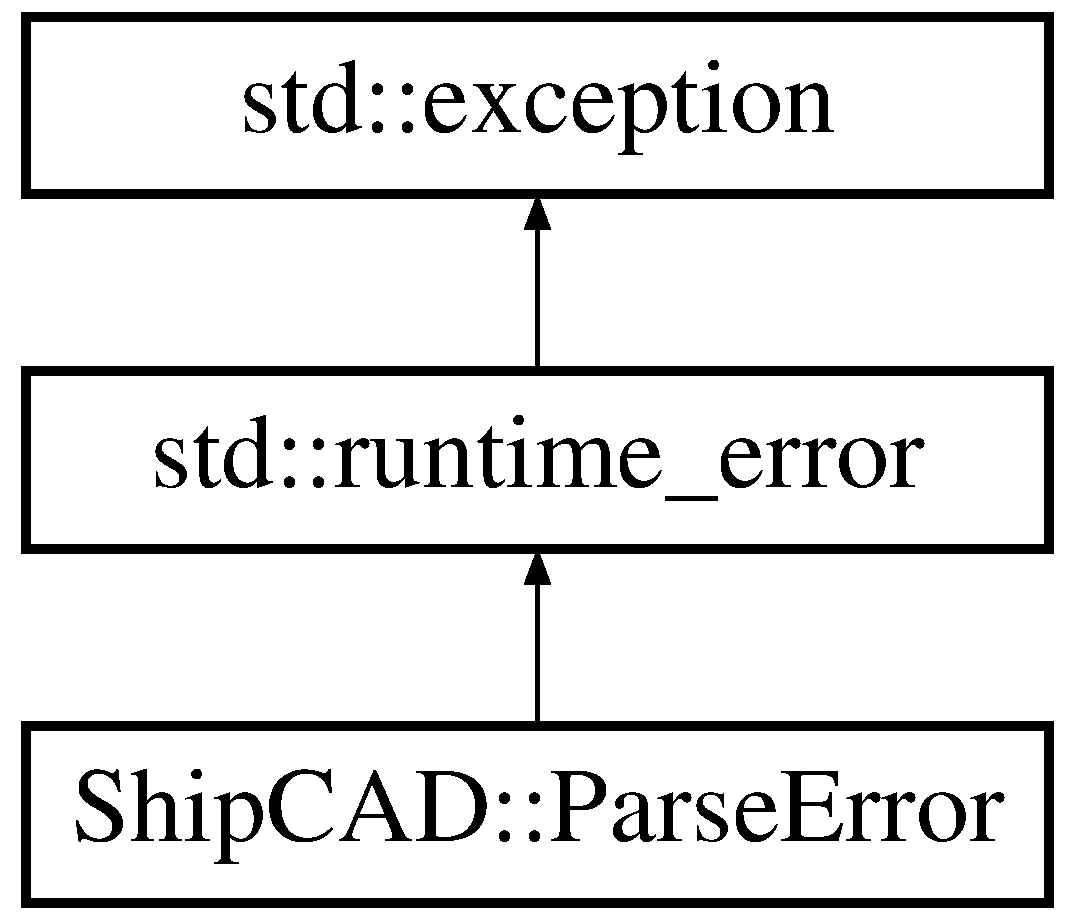
\includegraphics[height=3.000000cm]{classShipCAD_1_1ParseError}
\end{center}
\end{figure}
\subsection*{Public Member Functions}
\begin{DoxyCompactItemize}
\item 
\hyperlink{classShipCAD_1_1ParseError_aa4bb0213988602df68319e7dae54dfe6}{Parse\+Error} (size\+\_\+t linenum, const Q\+String \&\hyperlink{classShipCAD_1_1ParseError_adddab14352397af6868f8ab973108efa}{info})
\item 
const Q\+String \& \hyperlink{classShipCAD_1_1ParseError_adddab14352397af6868f8ab973108efa}{info} () const 
\item 
size\+\_\+t \hyperlink{classShipCAD_1_1ParseError_a572bd9bbbf1d7b6683c8a758a37be7a3}{lineno} () const 
\end{DoxyCompactItemize}


\subsection{Detailed Description}


Definition at line 39 of file exception.\+h.



\subsection{Constructor \& Destructor Documentation}
\index{Ship\+C\+A\+D\+::\+Parse\+Error@{Ship\+C\+A\+D\+::\+Parse\+Error}!Parse\+Error@{Parse\+Error}}
\index{Parse\+Error@{Parse\+Error}!Ship\+C\+A\+D\+::\+Parse\+Error@{Ship\+C\+A\+D\+::\+Parse\+Error}}
\subsubsection[{\texorpdfstring{Parse\+Error(size\+\_\+t linenum, const Q\+String \&info)}{ParseError(size_t linenum, const QString &info)}}]{\setlength{\rightskip}{0pt plus 5cm}Ship\+C\+A\+D\+::\+Parse\+Error\+::\+Parse\+Error (
\begin{DoxyParamCaption}
\item[{size\+\_\+t}]{linenum, }
\item[{const Q\+String \&}]{info}
\end{DoxyParamCaption}
)\hspace{0.3cm}{\ttfamily [inline]}}\hypertarget{classShipCAD_1_1ParseError_aa4bb0213988602df68319e7dae54dfe6}{}\label{classShipCAD_1_1ParseError_aa4bb0213988602df68319e7dae54dfe6}


Definition at line 42 of file exception.\+h.



\subsection{Member Function Documentation}
\index{Ship\+C\+A\+D\+::\+Parse\+Error@{Ship\+C\+A\+D\+::\+Parse\+Error}!info@{info}}
\index{info@{info}!Ship\+C\+A\+D\+::\+Parse\+Error@{Ship\+C\+A\+D\+::\+Parse\+Error}}
\subsubsection[{\texorpdfstring{info() const }{info() const }}]{\setlength{\rightskip}{0pt plus 5cm}const Q\+String\& Ship\+C\+A\+D\+::\+Parse\+Error\+::info (
\begin{DoxyParamCaption}
{}
\end{DoxyParamCaption}
) const\hspace{0.3cm}{\ttfamily [inline]}}\hypertarget{classShipCAD_1_1ParseError_adddab14352397af6868f8ab973108efa}{}\label{classShipCAD_1_1ParseError_adddab14352397af6868f8ab973108efa}


Definition at line 45 of file exception.\+h.

\index{Ship\+C\+A\+D\+::\+Parse\+Error@{Ship\+C\+A\+D\+::\+Parse\+Error}!lineno@{lineno}}
\index{lineno@{lineno}!Ship\+C\+A\+D\+::\+Parse\+Error@{Ship\+C\+A\+D\+::\+Parse\+Error}}
\subsubsection[{\texorpdfstring{lineno() const }{lineno() const }}]{\setlength{\rightskip}{0pt plus 5cm}size\+\_\+t Ship\+C\+A\+D\+::\+Parse\+Error\+::lineno (
\begin{DoxyParamCaption}
{}
\end{DoxyParamCaption}
) const\hspace{0.3cm}{\ttfamily [inline]}}\hypertarget{classShipCAD_1_1ParseError_a572bd9bbbf1d7b6683c8a758a37be7a3}{}\label{classShipCAD_1_1ParseError_a572bd9bbbf1d7b6683c8a758a37be7a3}


Definition at line 46 of file exception.\+h.



The documentation for this class was generated from the following file\+:\begin{DoxyCompactItemize}
\item 
Ship\+C\+A\+Dlib/\hyperlink{exception_8h}{exception.\+h}\end{DoxyCompactItemize}

\hypertarget{structPatchIntersection}{}\section{Patch\+Intersection Struct Reference}
\label{structPatchIntersection}\index{Patch\+Intersection@{Patch\+Intersection}}
\subsection*{Public Attributes}
\begin{DoxyCompactItemize}
\item 
Q\+Vector3D \hyperlink{structPatchIntersection_ada1d0adcd4dbc07d37a1676ac3c89cf0}{point}
\item 
bool \hyperlink{structPatchIntersection_a328e33e74b1d1904db5d69fd512b7d5c}{knuckle}
\end{DoxyCompactItemize}


\subsection{Detailed Description}


Definition at line 195 of file developedpatch.\+cpp.



\subsection{Member Data Documentation}
\index{Patch\+Intersection@{Patch\+Intersection}!knuckle@{knuckle}}
\index{knuckle@{knuckle}!Patch\+Intersection@{Patch\+Intersection}}
\subsubsection[{\texorpdfstring{knuckle}{knuckle}}]{\setlength{\rightskip}{0pt plus 5cm}bool Patch\+Intersection\+::knuckle}\hypertarget{structPatchIntersection_a328e33e74b1d1904db5d69fd512b7d5c}{}\label{structPatchIntersection_a328e33e74b1d1904db5d69fd512b7d5c}


Definition at line 198 of file developedpatch.\+cpp.

\index{Patch\+Intersection@{Patch\+Intersection}!point@{point}}
\index{point@{point}!Patch\+Intersection@{Patch\+Intersection}}
\subsubsection[{\texorpdfstring{point}{point}}]{\setlength{\rightskip}{0pt plus 5cm}Q\+Vector3D Patch\+Intersection\+::point}\hypertarget{structPatchIntersection_ada1d0adcd4dbc07d37a1676ac3c89cf0}{}\label{structPatchIntersection_ada1d0adcd4dbc07d37a1676ac3c89cf0}


Definition at line 197 of file developedpatch.\+cpp.



The documentation for this struct was generated from the following file\+:\begin{DoxyCompactItemize}
\item 
Ship\+C\+A\+Dlib/\hyperlink{developedpatch_8cpp}{developedpatch.\+cpp}\end{DoxyCompactItemize}

\hypertarget{structPatchPointPred}{}\section{Patch\+Point\+Pred Struct Reference}
\label{structPatchPointPred}\index{Patch\+Point\+Pred@{Patch\+Point\+Pred}}
\subsection*{Public Member Functions}
\begin{DoxyCompactItemize}
\item 
bool \hyperlink{structPatchPointPred_a5c23625bf138fee4f16dadcb172eece5}{operator()} (const \hyperlink{structShipCAD_1_1PatchPoints}{Ship\+C\+A\+D\+::\+Patch\+Points} \&val)
\item 
\hyperlink{structPatchPointPred_a981ff7bab687bc4c7b7342bb911e0858}{Patch\+Point\+Pred} (\hyperlink{classShipCAD_1_1SubdivisionPoint}{Ship\+C\+A\+D\+::\+Subdivision\+Point} $\ast$pt)
\end{DoxyCompactItemize}
\subsection*{Public Attributes}
\begin{DoxyCompactItemize}
\item 
\hyperlink{classShipCAD_1_1SubdivisionPoint}{Ship\+C\+A\+D\+::\+Subdivision\+Point} $\ast$ \hyperlink{structPatchPointPred_a79fcffc92b3f4411cc5f037a87cbaf2e}{querypt}
\end{DoxyCompactItemize}


\subsection{Detailed Description}


Definition at line 202 of file developedpatch.\+cpp.



\subsection{Constructor \& Destructor Documentation}
\index{Patch\+Point\+Pred@{Patch\+Point\+Pred}!Patch\+Point\+Pred@{Patch\+Point\+Pred}}
\index{Patch\+Point\+Pred@{Patch\+Point\+Pred}!Patch\+Point\+Pred@{Patch\+Point\+Pred}}
\subsubsection[{\texorpdfstring{Patch\+Point\+Pred(\+Ship\+C\+A\+D\+::\+Subdivision\+Point $\ast$pt)}{PatchPointPred(ShipCAD::SubdivisionPoint *pt)}}]{\setlength{\rightskip}{0pt plus 5cm}Patch\+Point\+Pred\+::\+Patch\+Point\+Pred (
\begin{DoxyParamCaption}
\item[{{\bf Ship\+C\+A\+D\+::\+Subdivision\+Point} $\ast$}]{pt}
\end{DoxyParamCaption}
)\hspace{0.3cm}{\ttfamily [inline]}, {\ttfamily [explicit]}}\hypertarget{structPatchPointPred_a981ff7bab687bc4c7b7342bb911e0858}{}\label{structPatchPointPred_a981ff7bab687bc4c7b7342bb911e0858}


Definition at line 208 of file developedpatch.\+cpp.



\subsection{Member Function Documentation}
\index{Patch\+Point\+Pred@{Patch\+Point\+Pred}!operator()@{operator()}}
\index{operator()@{operator()}!Patch\+Point\+Pred@{Patch\+Point\+Pred}}
\subsubsection[{\texorpdfstring{operator()(const Ship\+C\+A\+D\+::\+Patch\+Points \&val)}{operator()(const ShipCAD::PatchPoints &val)}}]{\setlength{\rightskip}{0pt plus 5cm}bool Patch\+Point\+Pred\+::operator() (
\begin{DoxyParamCaption}
\item[{const {\bf Ship\+C\+A\+D\+::\+Patch\+Points} \&}]{val}
\end{DoxyParamCaption}
)\hspace{0.3cm}{\ttfamily [inline]}}\hypertarget{structPatchPointPred_a5c23625bf138fee4f16dadcb172eece5}{}\label{structPatchPointPred_a5c23625bf138fee4f16dadcb172eece5}


Definition at line 205 of file developedpatch.\+cpp.



\subsection{Member Data Documentation}
\index{Patch\+Point\+Pred@{Patch\+Point\+Pred}!querypt@{querypt}}
\index{querypt@{querypt}!Patch\+Point\+Pred@{Patch\+Point\+Pred}}
\subsubsection[{\texorpdfstring{querypt}{querypt}}]{\setlength{\rightskip}{0pt plus 5cm}{\bf Ship\+C\+A\+D\+::\+Subdivision\+Point}$\ast$ Patch\+Point\+Pred\+::querypt}\hypertarget{structPatchPointPred_a79fcffc92b3f4411cc5f037a87cbaf2e}{}\label{structPatchPointPred_a79fcffc92b3f4411cc5f037a87cbaf2e}


Definition at line 204 of file developedpatch.\+cpp.



The documentation for this struct was generated from the following file\+:\begin{DoxyCompactItemize}
\item 
Ship\+C\+A\+Dlib/\hyperlink{developedpatch_8cpp}{developedpatch.\+cpp}\end{DoxyCompactItemize}

\hypertarget{structShipCAD_1_1PatchPoints}{}\section{Ship\+C\+AD\+:\+:Patch\+Points Struct Reference}
\label{structShipCAD_1_1PatchPoints}\index{Ship\+C\+A\+D\+::\+Patch\+Points@{Ship\+C\+A\+D\+::\+Patch\+Points}}


Store \hyperlink{classShipCAD_1_1SubdivisionPoint}{Subdivision\+Point} to unrolled point mapping.  




{\ttfamily \#include $<$developedpatch.\+h$>$}

\subsection*{Public Attributes}
\begin{DoxyCompactItemize}
\item 
Q\+Vector2D \hyperlink{structShipCAD_1_1PatchPoints_abce4e4187927ae79ecd5aafd604c1785}{pt2D}
\item 
\hyperlink{classShipCAD_1_1SubdivisionPoint}{Subdivision\+Point} $\ast$ \hyperlink{structShipCAD_1_1PatchPoints_ac69ca0b5e51939979f4654afa3b210a9}{pt}
\item 
bool \hyperlink{structShipCAD_1_1PatchPoints_a2f52ed0dc9945823b211f9e067164dce}{processed}
\end{DoxyCompactItemize}


\subsection{Detailed Description}
Store \hyperlink{classShipCAD_1_1SubdivisionPoint}{Subdivision\+Point} to unrolled point mapping. 

Definition at line 56 of file developedpatch.\+h.



\subsection{Member Data Documentation}
\index{Ship\+C\+A\+D\+::\+Patch\+Points@{Ship\+C\+A\+D\+::\+Patch\+Points}!processed@{processed}}
\index{processed@{processed}!Ship\+C\+A\+D\+::\+Patch\+Points@{Ship\+C\+A\+D\+::\+Patch\+Points}}
\subsubsection[{\texorpdfstring{processed}{processed}}]{\setlength{\rightskip}{0pt plus 5cm}bool Ship\+C\+A\+D\+::\+Patch\+Points\+::processed}\hypertarget{structShipCAD_1_1PatchPoints_a2f52ed0dc9945823b211f9e067164dce}{}\label{structShipCAD_1_1PatchPoints_a2f52ed0dc9945823b211f9e067164dce}


Definition at line 60 of file developedpatch.\+h.

\index{Ship\+C\+A\+D\+::\+Patch\+Points@{Ship\+C\+A\+D\+::\+Patch\+Points}!pt@{pt}}
\index{pt@{pt}!Ship\+C\+A\+D\+::\+Patch\+Points@{Ship\+C\+A\+D\+::\+Patch\+Points}}
\subsubsection[{\texorpdfstring{pt}{pt}}]{\setlength{\rightskip}{0pt plus 5cm}{\bf Subdivision\+Point}$\ast$ Ship\+C\+A\+D\+::\+Patch\+Points\+::pt}\hypertarget{structShipCAD_1_1PatchPoints_ac69ca0b5e51939979f4654afa3b210a9}{}\label{structShipCAD_1_1PatchPoints_ac69ca0b5e51939979f4654afa3b210a9}


Definition at line 59 of file developedpatch.\+h.

\index{Ship\+C\+A\+D\+::\+Patch\+Points@{Ship\+C\+A\+D\+::\+Patch\+Points}!pt2D@{pt2D}}
\index{pt2D@{pt2D}!Ship\+C\+A\+D\+::\+Patch\+Points@{Ship\+C\+A\+D\+::\+Patch\+Points}}
\subsubsection[{\texorpdfstring{pt2D}{pt2D}}]{\setlength{\rightskip}{0pt plus 5cm}Q\+Vector2D Ship\+C\+A\+D\+::\+Patch\+Points\+::pt2D}\hypertarget{structShipCAD_1_1PatchPoints_abce4e4187927ae79ecd5aafd604c1785}{}\label{structShipCAD_1_1PatchPoints_abce4e4187927ae79ecd5aafd604c1785}


Definition at line 58 of file developedpatch.\+h.



The documentation for this struct was generated from the following file\+:\begin{DoxyCompactItemize}
\item 
Ship\+C\+A\+Dlib/\hyperlink{developedpatch_8h}{developedpatch.\+h}\end{DoxyCompactItemize}

\hypertarget{structShipCAD_1_1PickRay}{}\section{Ship\+C\+AD\+:\+:Pick\+Ray Struct Reference}
\label{structShipCAD_1_1PickRay}\index{Ship\+C\+A\+D\+::\+Pick\+Ray@{Ship\+C\+A\+D\+::\+Pick\+Ray}}


a pick ray (line)  




{\ttfamily \#include $<$shipcadlib.\+h$>$}

\subsection*{Public Member Functions}
\begin{DoxyCompactItemize}
\item 
\hyperlink{structShipCAD_1_1PickRay_a423b609ea367f578f4c8abc6638daec4}{Pick\+Ray} (bool multi, bool p, bool e, bool f)
\end{DoxyCompactItemize}
\subsection*{Public Attributes}
\begin{DoxyCompactItemize}
\item 
Q\+Vector3D \hyperlink{structShipCAD_1_1PickRay_a2a9ed44a643481ceefcdec276ce7425a}{pt}
\item 
Q\+Vector3D \hyperlink{structShipCAD_1_1PickRay_a9e277629b120f405d2780f1235e8dcb1}{dir}
\item 
float \hyperlink{structShipCAD_1_1PickRay_aea6c9d67dc7245b1edf930dfe019d4db}{pick\+Dist}
\item 
bool \hyperlink{structShipCAD_1_1PickRay_a5b5dbf3de2afc804978a5e35ac582028}{multi\+\_\+sel}
\item 
bool \hyperlink{structShipCAD_1_1PickRay_a6576863fe4c5cb5eaa5ebcaa474104c8}{point}
\item 
bool \hyperlink{structShipCAD_1_1PickRay_a9882c4e0e43e2141cbaa196fe109cf19}{edge}
\item 
bool \hyperlink{structShipCAD_1_1PickRay_a76218677660d84089b3db5a137410cec}{face}
\end{DoxyCompactItemize}


\subsection{Detailed Description}
a pick ray (line) 

Definition at line 171 of file shipcadlib.\+h.



\subsection{Constructor \& Destructor Documentation}
\index{Ship\+C\+A\+D\+::\+Pick\+Ray@{Ship\+C\+A\+D\+::\+Pick\+Ray}!Pick\+Ray@{Pick\+Ray}}
\index{Pick\+Ray@{Pick\+Ray}!Ship\+C\+A\+D\+::\+Pick\+Ray@{Ship\+C\+A\+D\+::\+Pick\+Ray}}
\subsubsection[{\texorpdfstring{Pick\+Ray(bool multi, bool p, bool e, bool f)}{PickRay(bool multi, bool p, bool e, bool f)}}]{\setlength{\rightskip}{0pt plus 5cm}Ship\+C\+A\+D\+::\+Pick\+Ray\+::\+Pick\+Ray (
\begin{DoxyParamCaption}
\item[{bool}]{multi, }
\item[{bool}]{p, }
\item[{bool}]{e, }
\item[{bool}]{f}
\end{DoxyParamCaption}
)\hspace{0.3cm}{\ttfamily [inline]}}\hypertarget{structShipCAD_1_1PickRay_a423b609ea367f578f4c8abc6638daec4}{}\label{structShipCAD_1_1PickRay_a423b609ea367f578f4c8abc6638daec4}


Definition at line 180 of file shipcadlib.\+h.



\subsection{Member Data Documentation}
\index{Ship\+C\+A\+D\+::\+Pick\+Ray@{Ship\+C\+A\+D\+::\+Pick\+Ray}!dir@{dir}}
\index{dir@{dir}!Ship\+C\+A\+D\+::\+Pick\+Ray@{Ship\+C\+A\+D\+::\+Pick\+Ray}}
\subsubsection[{\texorpdfstring{dir}{dir}}]{\setlength{\rightskip}{0pt plus 5cm}Q\+Vector3D Ship\+C\+A\+D\+::\+Pick\+Ray\+::dir}\hypertarget{structShipCAD_1_1PickRay_a9e277629b120f405d2780f1235e8dcb1}{}\label{structShipCAD_1_1PickRay_a9e277629b120f405d2780f1235e8dcb1}


Definition at line 174 of file shipcadlib.\+h.

\index{Ship\+C\+A\+D\+::\+Pick\+Ray@{Ship\+C\+A\+D\+::\+Pick\+Ray}!edge@{edge}}
\index{edge@{edge}!Ship\+C\+A\+D\+::\+Pick\+Ray@{Ship\+C\+A\+D\+::\+Pick\+Ray}}
\subsubsection[{\texorpdfstring{edge}{edge}}]{\setlength{\rightskip}{0pt plus 5cm}bool Ship\+C\+A\+D\+::\+Pick\+Ray\+::edge}\hypertarget{structShipCAD_1_1PickRay_a9882c4e0e43e2141cbaa196fe109cf19}{}\label{structShipCAD_1_1PickRay_a9882c4e0e43e2141cbaa196fe109cf19}


Definition at line 178 of file shipcadlib.\+h.

\index{Ship\+C\+A\+D\+::\+Pick\+Ray@{Ship\+C\+A\+D\+::\+Pick\+Ray}!face@{face}}
\index{face@{face}!Ship\+C\+A\+D\+::\+Pick\+Ray@{Ship\+C\+A\+D\+::\+Pick\+Ray}}
\subsubsection[{\texorpdfstring{face}{face}}]{\setlength{\rightskip}{0pt plus 5cm}bool Ship\+C\+A\+D\+::\+Pick\+Ray\+::face}\hypertarget{structShipCAD_1_1PickRay_a76218677660d84089b3db5a137410cec}{}\label{structShipCAD_1_1PickRay_a76218677660d84089b3db5a137410cec}


Definition at line 179 of file shipcadlib.\+h.

\index{Ship\+C\+A\+D\+::\+Pick\+Ray@{Ship\+C\+A\+D\+::\+Pick\+Ray}!multi\+\_\+sel@{multi\+\_\+sel}}
\index{multi\+\_\+sel@{multi\+\_\+sel}!Ship\+C\+A\+D\+::\+Pick\+Ray@{Ship\+C\+A\+D\+::\+Pick\+Ray}}
\subsubsection[{\texorpdfstring{multi\+\_\+sel}{multi_sel}}]{\setlength{\rightskip}{0pt plus 5cm}bool Ship\+C\+A\+D\+::\+Pick\+Ray\+::multi\+\_\+sel}\hypertarget{structShipCAD_1_1PickRay_a5b5dbf3de2afc804978a5e35ac582028}{}\label{structShipCAD_1_1PickRay_a5b5dbf3de2afc804978a5e35ac582028}


Definition at line 176 of file shipcadlib.\+h.

\index{Ship\+C\+A\+D\+::\+Pick\+Ray@{Ship\+C\+A\+D\+::\+Pick\+Ray}!pick\+Dist@{pick\+Dist}}
\index{pick\+Dist@{pick\+Dist}!Ship\+C\+A\+D\+::\+Pick\+Ray@{Ship\+C\+A\+D\+::\+Pick\+Ray}}
\subsubsection[{\texorpdfstring{pick\+Dist}{pickDist}}]{\setlength{\rightskip}{0pt plus 5cm}float Ship\+C\+A\+D\+::\+Pick\+Ray\+::pick\+Dist}\hypertarget{structShipCAD_1_1PickRay_aea6c9d67dc7245b1edf930dfe019d4db}{}\label{structShipCAD_1_1PickRay_aea6c9d67dc7245b1edf930dfe019d4db}


Definition at line 175 of file shipcadlib.\+h.

\index{Ship\+C\+A\+D\+::\+Pick\+Ray@{Ship\+C\+A\+D\+::\+Pick\+Ray}!point@{point}}
\index{point@{point}!Ship\+C\+A\+D\+::\+Pick\+Ray@{Ship\+C\+A\+D\+::\+Pick\+Ray}}
\subsubsection[{\texorpdfstring{point}{point}}]{\setlength{\rightskip}{0pt plus 5cm}bool Ship\+C\+A\+D\+::\+Pick\+Ray\+::point}\hypertarget{structShipCAD_1_1PickRay_a6576863fe4c5cb5eaa5ebcaa474104c8}{}\label{structShipCAD_1_1PickRay_a6576863fe4c5cb5eaa5ebcaa474104c8}


Definition at line 177 of file shipcadlib.\+h.

\index{Ship\+C\+A\+D\+::\+Pick\+Ray@{Ship\+C\+A\+D\+::\+Pick\+Ray}!pt@{pt}}
\index{pt@{pt}!Ship\+C\+A\+D\+::\+Pick\+Ray@{Ship\+C\+A\+D\+::\+Pick\+Ray}}
\subsubsection[{\texorpdfstring{pt}{pt}}]{\setlength{\rightskip}{0pt plus 5cm}Q\+Vector3D Ship\+C\+A\+D\+::\+Pick\+Ray\+::pt}\hypertarget{structShipCAD_1_1PickRay_a2a9ed44a643481ceefcdec276ce7425a}{}\label{structShipCAD_1_1PickRay_a2a9ed44a643481ceefcdec276ce7425a}


Definition at line 173 of file shipcadlib.\+h.



The documentation for this struct was generated from the following file\+:\begin{DoxyCompactItemize}
\item 
Ship\+C\+A\+Dlib/\hyperlink{shipcadlib_8h}{shipcadlib.\+h}\end{DoxyCompactItemize}

\hypertarget{classShipCAD_1_1Plane}{}\section{Ship\+C\+AD\+:\+:Plane Class Reference}
\label{classShipCAD_1_1Plane}\index{Ship\+C\+A\+D\+::\+Plane@{Ship\+C\+A\+D\+::\+Plane}}


{\ttfamily \#include $<$plane.\+h$>$}

\subsection*{Public Member Functions}
\begin{DoxyCompactItemize}
\item 
\hyperlink{classShipCAD_1_1Plane_acac0d9c003e0ab10d07b146c3566a0c7}{Plane} ()
\item 
\hyperlink{classShipCAD_1_1Plane_a9a1420228e8baa632c7e8ba66f27772f}{Plane} (float \hyperlink{classShipCAD_1_1Plane_a1105f3715d9593c0971e0b0959859a84}{a}, float \hyperlink{classShipCAD_1_1Plane_adf79c9ba86dd3112fc098141195fcac5}{b}, float \hyperlink{classShipCAD_1_1Plane_a01b0067ca1a669aef5a8ab85bfce41cc}{c}, float \hyperlink{classShipCAD_1_1Plane_a7755d7967aae2e083c5d08fed49d9eef}{d})
\item 
\hyperlink{classShipCAD_1_1Plane_a254ddea0d760646007a19512e502e6fc}{Plane} (const Q\+Vector3D \&p, const Q\+Vector3D \&normal)
\item 
\hyperlink{classShipCAD_1_1Plane_adbaa1f5c7100e5592312359cb8eede37}{Plane} (const Q\+Vector3D \&p1, const Q\+Vector3D \&p2, const Q\+Vector3D \&p3)
\item 
\hyperlink{classShipCAD_1_1Plane_aff2204f8b2b25c201d172d4ec2518c77}{$\sim$\+Plane} ()
\item 
float \hyperlink{classShipCAD_1_1Plane_a1105f3715d9593c0971e0b0959859a84}{a} () const 
\item 
float \hyperlink{classShipCAD_1_1Plane_adf79c9ba86dd3112fc098141195fcac5}{b} () const 
\item 
float \hyperlink{classShipCAD_1_1Plane_a01b0067ca1a669aef5a8ab85bfce41cc}{c} () const 
\item 
float \hyperlink{classShipCAD_1_1Plane_a7755d7967aae2e083c5d08fed49d9eef}{d} () const 
\item 
void \hyperlink{classShipCAD_1_1Plane_a383a2f49031b8bcfa04be06035836a05}{setA} (float val)
\item 
void \hyperlink{classShipCAD_1_1Plane_aab7d46cba75a32089644b183e0a82dff}{setB} (float val)
\item 
void \hyperlink{classShipCAD_1_1Plane_affed6efd889f4725ae764b243763fb3e}{setC} (float val)
\item 
void \hyperlink{classShipCAD_1_1Plane_a5c3e18bcb1bb77563fd994866ba823df}{setD} (float val)
\item 
float \hyperlink{classShipCAD_1_1Plane_a6851b997a300848fcb37b33407165c44}{distance} (const Q\+Vector3D \&point) const 
\item 
bool \hyperlink{classShipCAD_1_1Plane_a76d5f22d213962e8ab0880fae3e919df}{intersects\+Box} (const Q\+Vector3D \&p1, const Q\+Vector3D \&p2) const 
\item 
Q\+Vector3D \hyperlink{classShipCAD_1_1Plane_a2ef81e9310257ad80b087181f3191b4a}{project\+Point\+On\+Plane} (const Q\+Vector3D \&p) const 
\begin{DoxyCompactList}\small\item\em project a point onto a plane \end{DoxyCompactList}\item 
bool \hyperlink{classShipCAD_1_1Plane_a8f6c0ea64a798798ee098658cd38935b}{intersect\+Line} (const Q\+Vector3D \&pt, const Q\+Vector3D \&n, bool \&coplanar, Q\+Vector3D \&intpt) const 
\begin{DoxyCompactList}\small\item\em intersect a line with this plane \end{DoxyCompactList}\item 
Q\+Vector3D \hyperlink{classShipCAD_1_1Plane_a77073798d61488aeac1ebe95358e3b98}{mirror} (const Q\+Vector3D \&pt) const 
\begin{DoxyCompactList}\small\item\em get the mirror of a point about the plane \end{DoxyCompactList}\end{DoxyCompactItemize}


\subsection{Detailed Description}


Definition at line 39 of file plane.\+h.



\subsection{Constructor \& Destructor Documentation}
\index{Ship\+C\+A\+D\+::\+Plane@{Ship\+C\+A\+D\+::\+Plane}!Plane@{Plane}}
\index{Plane@{Plane}!Ship\+C\+A\+D\+::\+Plane@{Ship\+C\+A\+D\+::\+Plane}}
\subsubsection[{\texorpdfstring{Plane()}{Plane()}}]{\setlength{\rightskip}{0pt plus 5cm}Plane\+::\+Plane (
\begin{DoxyParamCaption}
{}
\end{DoxyParamCaption}
)\hspace{0.3cm}{\ttfamily [explicit]}}\hypertarget{classShipCAD_1_1Plane_acac0d9c003e0ab10d07b146c3566a0c7}{}\label{classShipCAD_1_1Plane_acac0d9c003e0ab10d07b146c3566a0c7}


Definition at line 37 of file plane.\+cpp.

\index{Ship\+C\+A\+D\+::\+Plane@{Ship\+C\+A\+D\+::\+Plane}!Plane@{Plane}}
\index{Plane@{Plane}!Ship\+C\+A\+D\+::\+Plane@{Ship\+C\+A\+D\+::\+Plane}}
\subsubsection[{\texorpdfstring{Plane(float a, float b, float c, float d)}{Plane(float a, float b, float c, float d)}}]{\setlength{\rightskip}{0pt plus 5cm}Plane\+::\+Plane (
\begin{DoxyParamCaption}
\item[{float}]{a, }
\item[{float}]{b, }
\item[{float}]{c, }
\item[{float}]{d}
\end{DoxyParamCaption}
)\hspace{0.3cm}{\ttfamily [explicit]}}\hypertarget{classShipCAD_1_1Plane_a9a1420228e8baa632c7e8ba66f27772f}{}\label{classShipCAD_1_1Plane_a9a1420228e8baa632c7e8ba66f27772f}


Definition at line 42 of file plane.\+cpp.

\index{Ship\+C\+A\+D\+::\+Plane@{Ship\+C\+A\+D\+::\+Plane}!Plane@{Plane}}
\index{Plane@{Plane}!Ship\+C\+A\+D\+::\+Plane@{Ship\+C\+A\+D\+::\+Plane}}
\subsubsection[{\texorpdfstring{Plane(const Q\+Vector3\+D \&p, const Q\+Vector3\+D \&normal)}{Plane(const QVector3D &p, const QVector3D &normal)}}]{\setlength{\rightskip}{0pt plus 5cm}Plane\+::\+Plane (
\begin{DoxyParamCaption}
\item[{const Q\+Vector3D \&}]{p, }
\item[{const Q\+Vector3D \&}]{normal}
\end{DoxyParamCaption}
)\hspace{0.3cm}{\ttfamily [explicit]}}\hypertarget{classShipCAD_1_1Plane_a254ddea0d760646007a19512e502e6fc}{}\label{classShipCAD_1_1Plane_a254ddea0d760646007a19512e502e6fc}


Definition at line 50 of file plane.\+cpp.

\index{Ship\+C\+A\+D\+::\+Plane@{Ship\+C\+A\+D\+::\+Plane}!Plane@{Plane}}
\index{Plane@{Plane}!Ship\+C\+A\+D\+::\+Plane@{Ship\+C\+A\+D\+::\+Plane}}
\subsubsection[{\texorpdfstring{Plane(const Q\+Vector3\+D \&p1, const Q\+Vector3\+D \&p2, const Q\+Vector3\+D \&p3)}{Plane(const QVector3D &p1, const QVector3D &p2, const QVector3D &p3)}}]{\setlength{\rightskip}{0pt plus 5cm}Plane\+::\+Plane (
\begin{DoxyParamCaption}
\item[{const Q\+Vector3D \&}]{p1, }
\item[{const Q\+Vector3D \&}]{p2, }
\item[{const Q\+Vector3D \&}]{p3}
\end{DoxyParamCaption}
)\hspace{0.3cm}{\ttfamily [explicit]}}\hypertarget{classShipCAD_1_1Plane_adbaa1f5c7100e5592312359cb8eede37}{}\label{classShipCAD_1_1Plane_adbaa1f5c7100e5592312359cb8eede37}


Definition at line 58 of file plane.\+cpp.

\index{Ship\+C\+A\+D\+::\+Plane@{Ship\+C\+A\+D\+::\+Plane}!````~Plane@{$\sim$\+Plane}}
\index{````~Plane@{$\sim$\+Plane}!Ship\+C\+A\+D\+::\+Plane@{Ship\+C\+A\+D\+::\+Plane}}
\subsubsection[{\texorpdfstring{$\sim$\+Plane()}{~Plane()}}]{\setlength{\rightskip}{0pt plus 5cm}Ship\+C\+A\+D\+::\+Plane\+::$\sim$\+Plane (
\begin{DoxyParamCaption}
{}
\end{DoxyParamCaption}
)\hspace{0.3cm}{\ttfamily [inline]}}\hypertarget{classShipCAD_1_1Plane_aff2204f8b2b25c201d172d4ec2518c77}{}\label{classShipCAD_1_1Plane_aff2204f8b2b25c201d172d4ec2518c77}


Definition at line 48 of file plane.\+h.



\subsection{Member Function Documentation}
\index{Ship\+C\+A\+D\+::\+Plane@{Ship\+C\+A\+D\+::\+Plane}!a@{a}}
\index{a@{a}!Ship\+C\+A\+D\+::\+Plane@{Ship\+C\+A\+D\+::\+Plane}}
\subsubsection[{\texorpdfstring{a() const }{a() const }}]{\setlength{\rightskip}{0pt plus 5cm}float Ship\+C\+A\+D\+::\+Plane\+::a (
\begin{DoxyParamCaption}
{}
\end{DoxyParamCaption}
) const\hspace{0.3cm}{\ttfamily [inline]}}\hypertarget{classShipCAD_1_1Plane_a1105f3715d9593c0971e0b0959859a84}{}\label{classShipCAD_1_1Plane_a1105f3715d9593c0971e0b0959859a84}


Definition at line 50 of file plane.\+h.

\index{Ship\+C\+A\+D\+::\+Plane@{Ship\+C\+A\+D\+::\+Plane}!b@{b}}
\index{b@{b}!Ship\+C\+A\+D\+::\+Plane@{Ship\+C\+A\+D\+::\+Plane}}
\subsubsection[{\texorpdfstring{b() const }{b() const }}]{\setlength{\rightskip}{0pt plus 5cm}float Ship\+C\+A\+D\+::\+Plane\+::b (
\begin{DoxyParamCaption}
{}
\end{DoxyParamCaption}
) const\hspace{0.3cm}{\ttfamily [inline]}}\hypertarget{classShipCAD_1_1Plane_adf79c9ba86dd3112fc098141195fcac5}{}\label{classShipCAD_1_1Plane_adf79c9ba86dd3112fc098141195fcac5}


Definition at line 52 of file plane.\+h.

\index{Ship\+C\+A\+D\+::\+Plane@{Ship\+C\+A\+D\+::\+Plane}!c@{c}}
\index{c@{c}!Ship\+C\+A\+D\+::\+Plane@{Ship\+C\+A\+D\+::\+Plane}}
\subsubsection[{\texorpdfstring{c() const }{c() const }}]{\setlength{\rightskip}{0pt plus 5cm}float Ship\+C\+A\+D\+::\+Plane\+::c (
\begin{DoxyParamCaption}
{}
\end{DoxyParamCaption}
) const\hspace{0.3cm}{\ttfamily [inline]}}\hypertarget{classShipCAD_1_1Plane_a01b0067ca1a669aef5a8ab85bfce41cc}{}\label{classShipCAD_1_1Plane_a01b0067ca1a669aef5a8ab85bfce41cc}


Definition at line 54 of file plane.\+h.

\index{Ship\+C\+A\+D\+::\+Plane@{Ship\+C\+A\+D\+::\+Plane}!d@{d}}
\index{d@{d}!Ship\+C\+A\+D\+::\+Plane@{Ship\+C\+A\+D\+::\+Plane}}
\subsubsection[{\texorpdfstring{d() const }{d() const }}]{\setlength{\rightskip}{0pt plus 5cm}float Ship\+C\+A\+D\+::\+Plane\+::d (
\begin{DoxyParamCaption}
{}
\end{DoxyParamCaption}
) const\hspace{0.3cm}{\ttfamily [inline]}}\hypertarget{classShipCAD_1_1Plane_a7755d7967aae2e083c5d08fed49d9eef}{}\label{classShipCAD_1_1Plane_a7755d7967aae2e083c5d08fed49d9eef}


Definition at line 56 of file plane.\+h.

\index{Ship\+C\+A\+D\+::\+Plane@{Ship\+C\+A\+D\+::\+Plane}!distance@{distance}}
\index{distance@{distance}!Ship\+C\+A\+D\+::\+Plane@{Ship\+C\+A\+D\+::\+Plane}}
\subsubsection[{\texorpdfstring{distance(const Q\+Vector3\+D \&point) const }{distance(const QVector3D &point) const }}]{\setlength{\rightskip}{0pt plus 5cm}float Plane\+::distance (
\begin{DoxyParamCaption}
\item[{const Q\+Vector3D \&}]{point}
\end{DoxyParamCaption}
) const}\hypertarget{classShipCAD_1_1Plane_a6851b997a300848fcb37b33407165c44}{}\label{classShipCAD_1_1Plane_a6851b997a300848fcb37b33407165c44}


Definition at line 72 of file plane.\+cpp.

\index{Ship\+C\+A\+D\+::\+Plane@{Ship\+C\+A\+D\+::\+Plane}!intersect\+Line@{intersect\+Line}}
\index{intersect\+Line@{intersect\+Line}!Ship\+C\+A\+D\+::\+Plane@{Ship\+C\+A\+D\+::\+Plane}}
\subsubsection[{\texorpdfstring{intersect\+Line(const Q\+Vector3\+D \&pt, const Q\+Vector3\+D \&n, bool \&coplanar, Q\+Vector3\+D \&intpt) const }{intersectLine(const QVector3D &pt, const QVector3D &n, bool &coplanar, QVector3D &intpt) const }}]{\setlength{\rightskip}{0pt plus 5cm}bool Plane\+::intersect\+Line (
\begin{DoxyParamCaption}
\item[{const Q\+Vector3D \&}]{pt, }
\item[{const Q\+Vector3D \&}]{n, }
\item[{bool \&}]{coplanar, }
\item[{Q\+Vector3D \&}]{intpt}
\end{DoxyParamCaption}
) const}\hypertarget{classShipCAD_1_1Plane_a8f6c0ea64a798798ee098658cd38935b}{}\label{classShipCAD_1_1Plane_a8f6c0ea64a798798ee098658cd38935b}


intersect a line with this plane 


\begin{DoxyParams}{Parameters}
{\em pt} & point on line \\
\hline
{\em n} & direction of line \\
\hline
{\em coplanar} & will be true if line lies in the plane \\
\hline
{\em intpt} & intersection point \\
\hline
\end{DoxyParams}
\begin{DoxyReturn}{Returns}
true if line and plane are parallel 
\end{DoxyReturn}


Definition at line 136 of file plane.\+cpp.

\index{Ship\+C\+A\+D\+::\+Plane@{Ship\+C\+A\+D\+::\+Plane}!intersects\+Box@{intersects\+Box}}
\index{intersects\+Box@{intersects\+Box}!Ship\+C\+A\+D\+::\+Plane@{Ship\+C\+A\+D\+::\+Plane}}
\subsubsection[{\texorpdfstring{intersects\+Box(const Q\+Vector3\+D \&p1, const Q\+Vector3\+D \&p2) const }{intersectsBox(const QVector3D &p1, const QVector3D &p2) const }}]{\setlength{\rightskip}{0pt plus 5cm}bool Plane\+::intersects\+Box (
\begin{DoxyParamCaption}
\item[{const Q\+Vector3D \&}]{p1, }
\item[{const Q\+Vector3D \&}]{p2}
\end{DoxyParamCaption}
) const}\hypertarget{classShipCAD_1_1Plane_a76d5f22d213962e8ab0880fae3e919df}{}\label{classShipCAD_1_1Plane_a76d5f22d213962e8ab0880fae3e919df}


Definition at line 78 of file plane.\+cpp.

\index{Ship\+C\+A\+D\+::\+Plane@{Ship\+C\+A\+D\+::\+Plane}!mirror@{mirror}}
\index{mirror@{mirror}!Ship\+C\+A\+D\+::\+Plane@{Ship\+C\+A\+D\+::\+Plane}}
\subsubsection[{\texorpdfstring{mirror(const Q\+Vector3\+D \&pt) const }{mirror(const QVector3D &pt) const }}]{\setlength{\rightskip}{0pt plus 5cm}Q\+Vector3D Plane\+::mirror (
\begin{DoxyParamCaption}
\item[{const Q\+Vector3D \&}]{pt}
\end{DoxyParamCaption}
) const}\hypertarget{classShipCAD_1_1Plane_a77073798d61488aeac1ebe95358e3b98}{}\label{classShipCAD_1_1Plane_a77073798d61488aeac1ebe95358e3b98}


get the mirror of a point about the plane 


\begin{DoxyParams}{Parameters}
{\em pt} & point to mirror \\
\hline
\end{DoxyParams}
\begin{DoxyReturn}{Returns}
the mirrored point 
\end{DoxyReturn}


Definition at line 153 of file plane.\+cpp.

\index{Ship\+C\+A\+D\+::\+Plane@{Ship\+C\+A\+D\+::\+Plane}!project\+Point\+On\+Plane@{project\+Point\+On\+Plane}}
\index{project\+Point\+On\+Plane@{project\+Point\+On\+Plane}!Ship\+C\+A\+D\+::\+Plane@{Ship\+C\+A\+D\+::\+Plane}}
\subsubsection[{\texorpdfstring{project\+Point\+On\+Plane(const Q\+Vector3\+D \&p) const }{projectPointOnPlane(const QVector3D &p) const }}]{\setlength{\rightskip}{0pt plus 5cm}Q\+Vector3D Plane\+::project\+Point\+On\+Plane (
\begin{DoxyParamCaption}
\item[{const Q\+Vector3D \&}]{p}
\end{DoxyParamCaption}
) const}\hypertarget{classShipCAD_1_1Plane_a2ef81e9310257ad80b087181f3191b4a}{}\label{classShipCAD_1_1Plane_a2ef81e9310257ad80b087181f3191b4a}


project a point onto a plane 


\begin{DoxyParams}{Parameters}
{\em p} & the point to project onto this plane \\
\hline
\end{DoxyParams}
\begin{DoxyReturn}{Returns}
the projected point 
\end{DoxyReturn}


Definition at line 124 of file plane.\+cpp.

\index{Ship\+C\+A\+D\+::\+Plane@{Ship\+C\+A\+D\+::\+Plane}!setA@{setA}}
\index{setA@{setA}!Ship\+C\+A\+D\+::\+Plane@{Ship\+C\+A\+D\+::\+Plane}}
\subsubsection[{\texorpdfstring{set\+A(float val)}{setA(float val)}}]{\setlength{\rightskip}{0pt plus 5cm}void Ship\+C\+A\+D\+::\+Plane\+::setA (
\begin{DoxyParamCaption}
\item[{float}]{val}
\end{DoxyParamCaption}
)\hspace{0.3cm}{\ttfamily [inline]}}\hypertarget{classShipCAD_1_1Plane_a383a2f49031b8bcfa04be06035836a05}{}\label{classShipCAD_1_1Plane_a383a2f49031b8bcfa04be06035836a05}


Definition at line 59 of file plane.\+h.

\index{Ship\+C\+A\+D\+::\+Plane@{Ship\+C\+A\+D\+::\+Plane}!setB@{setB}}
\index{setB@{setB}!Ship\+C\+A\+D\+::\+Plane@{Ship\+C\+A\+D\+::\+Plane}}
\subsubsection[{\texorpdfstring{set\+B(float val)}{setB(float val)}}]{\setlength{\rightskip}{0pt plus 5cm}void Ship\+C\+A\+D\+::\+Plane\+::setB (
\begin{DoxyParamCaption}
\item[{float}]{val}
\end{DoxyParamCaption}
)\hspace{0.3cm}{\ttfamily [inline]}}\hypertarget{classShipCAD_1_1Plane_aab7d46cba75a32089644b183e0a82dff}{}\label{classShipCAD_1_1Plane_aab7d46cba75a32089644b183e0a82dff}


Definition at line 62 of file plane.\+h.

\index{Ship\+C\+A\+D\+::\+Plane@{Ship\+C\+A\+D\+::\+Plane}!setC@{setC}}
\index{setC@{setC}!Ship\+C\+A\+D\+::\+Plane@{Ship\+C\+A\+D\+::\+Plane}}
\subsubsection[{\texorpdfstring{set\+C(float val)}{setC(float val)}}]{\setlength{\rightskip}{0pt plus 5cm}void Ship\+C\+A\+D\+::\+Plane\+::setC (
\begin{DoxyParamCaption}
\item[{float}]{val}
\end{DoxyParamCaption}
)\hspace{0.3cm}{\ttfamily [inline]}}\hypertarget{classShipCAD_1_1Plane_affed6efd889f4725ae764b243763fb3e}{}\label{classShipCAD_1_1Plane_affed6efd889f4725ae764b243763fb3e}


Definition at line 65 of file plane.\+h.

\index{Ship\+C\+A\+D\+::\+Plane@{Ship\+C\+A\+D\+::\+Plane}!setD@{setD}}
\index{setD@{setD}!Ship\+C\+A\+D\+::\+Plane@{Ship\+C\+A\+D\+::\+Plane}}
\subsubsection[{\texorpdfstring{set\+D(float val)}{setD(float val)}}]{\setlength{\rightskip}{0pt plus 5cm}void Ship\+C\+A\+D\+::\+Plane\+::setD (
\begin{DoxyParamCaption}
\item[{float}]{val}
\end{DoxyParamCaption}
)\hspace{0.3cm}{\ttfamily [inline]}}\hypertarget{classShipCAD_1_1Plane_a5c3e18bcb1bb77563fd994866ba823df}{}\label{classShipCAD_1_1Plane_a5c3e18bcb1bb77563fd994866ba823df}


Definition at line 68 of file plane.\+h.



The documentation for this class was generated from the following files\+:\begin{DoxyCompactItemize}
\item 
Ship\+C\+A\+Dlib/\hyperlink{plane_8h}{plane.\+h}\item 
Ship\+C\+A\+Dlib/\hyperlink{plane_8cpp}{plane.\+cpp}\end{DoxyCompactItemize}

\hypertarget{structPointData}{}\section{Point\+Data Struct Reference}
\label{structPointData}\index{Point\+Data@{Point\+Data}}
\subsection*{Public Attributes}
\begin{DoxyCompactItemize}
\item 
Q\+Vector3D \hyperlink{structPointData_a36b2f6a6c661e48f0ca5fade9d01372c}{coord}
\item 
Q\+Vector3D \hyperlink{structPointData_a605965356cbc5e71fea58fd30605bba8}{flowdir}
\item 
vector$<$ size\+\_\+t $>$ \hyperlink{structPointData_a7de97589578b881bc7850ac0053c8613}{triangles}
\end{DoxyCompactItemize}


\subsection{Detailed Description}


Definition at line 166 of file flowline.\+cpp.



\subsection{Member Data Documentation}
\index{Point\+Data@{Point\+Data}!coord@{coord}}
\index{coord@{coord}!Point\+Data@{Point\+Data}}
\subsubsection[{\texorpdfstring{coord}{coord}}]{\setlength{\rightskip}{0pt plus 5cm}Q\+Vector3D Point\+Data\+::coord}\hypertarget{structPointData_a36b2f6a6c661e48f0ca5fade9d01372c}{}\label{structPointData_a36b2f6a6c661e48f0ca5fade9d01372c}


Definition at line 168 of file flowline.\+cpp.

\index{Point\+Data@{Point\+Data}!flowdir@{flowdir}}
\index{flowdir@{flowdir}!Point\+Data@{Point\+Data}}
\subsubsection[{\texorpdfstring{flowdir}{flowdir}}]{\setlength{\rightskip}{0pt plus 5cm}Q\+Vector3D Point\+Data\+::flowdir}\hypertarget{structPointData_a605965356cbc5e71fea58fd30605bba8}{}\label{structPointData_a605965356cbc5e71fea58fd30605bba8}


Definition at line 169 of file flowline.\+cpp.

\index{Point\+Data@{Point\+Data}!triangles@{triangles}}
\index{triangles@{triangles}!Point\+Data@{Point\+Data}}
\subsubsection[{\texorpdfstring{triangles}{triangles}}]{\setlength{\rightskip}{0pt plus 5cm}vector$<$size\+\_\+t$>$ Point\+Data\+::triangles}\hypertarget{structPointData_a7de97589578b881bc7850ac0053c8613}{}\label{structPointData_a7de97589578b881bc7850ac0053c8613}


Definition at line 170 of file flowline.\+cpp.



The documentation for this struct was generated from the following file\+:\begin{DoxyCompactItemize}
\item 
Ship\+C\+A\+Dlib/\hyperlink{flowline_8cpp}{flowline.\+cpp}\end{DoxyCompactItemize}

\hypertarget{classPointerVector}{}\section{Pointer\+Vector$<$ T $>$ Class Template Reference}
\label{classPointerVector}\index{Pointer\+Vector$<$ T $>$@{Pointer\+Vector$<$ T $>$}}


{\ttfamily \#include $<$pointervec.\+h$>$}

\subsection*{Public Types}
\begin{DoxyCompactItemize}
\item 
typedef void \hyperlink{classPointerVector_a578da527d71168684229a721b16e823f}{apply\+\_\+fn}(T $\ast$elem)
\end{DoxyCompactItemize}
\subsection*{Public Member Functions}
\begin{DoxyCompactItemize}
\item 
\hyperlink{classPointerVector_a44ef76bb36f22d17606d8af8ef12d499}{Pointer\+Vector} ()
\item 
\hyperlink{classPointerVector_ac1c5b843d7862e9db7189d459324e246}{Pointer\+Vector} (bool owned)
\item 
\hyperlink{classPointerVector_a5fd5c0d94cdb693be9a8bb5c2b3e305c}{$\sim$\+Pointer\+Vector} ()
\item 
void \hyperlink{classPointerVector_a9f708acfaa3ce26d14b02d8e285c8729}{clear} ()
\item 
size\+\_\+t \hyperlink{classPointerVector_a65263559ccd6a9eac2904c691453867b}{size} () const 
\item 
T $\ast$ \hyperlink{classPointerVector_af28c2517157ddacfb4d92a4fc73c5a92}{get} (size\+\_\+t index)
\item 
const T $\ast$ \hyperlink{classPointerVector_a298c14996c9995cc56efc2deadd01fe5}{get} (size\+\_\+t index) const 
\item 
void \hyperlink{classPointerVector_abaee9f77dee6ea2523dff64b184c9f54}{add} (T $\ast$elem)
\item 
bool \hyperlink{classPointerVector_acb88f3cb0aa36baaebabc0900bb304e6}{del} (T $\ast$elem)
\item 
void \hyperlink{classPointerVector_a5e9ccf28859f06f13ad3e2dad9ae1cb6}{apply} (\hyperlink{classPointerVector_a578da527d71168684229a721b16e823f}{apply\+\_\+fn} $\ast$fn)
\item 
std\+::vector$<$ T $\ast$ $>$\+::iterator \hyperlink{classPointerVector_a594866129f2e9a3701c1f414ca3299e3}{begin} ()
\item 
std\+::vector$<$ T $\ast$ $>$\+::iterator \hyperlink{classPointerVector_a6182f5429c4c98ba2556d40484aab2f9}{end} ()
\item 
std\+::vector$<$ T $\ast$ $>$\+::const\+\_\+iterator \hyperlink{classPointerVector_a97ee9f133fa9e61341f33feb3f36f45b}{begin} () const 
\item 
std\+::vector$<$ T $\ast$ $>$\+::const\+\_\+iterator \hyperlink{classPointerVector_a62f1573b2bdffb20efaad8fbff6d7676}{end} () const 
\item 
void \hyperlink{classPointerVector_a1107df98d34db68e3153e67196a16a11}{erase} (typename std\+::vector$<$ T $\ast$ $>$\+::iterator i)
\item 
void \hyperlink{classPointerVector_a0a7659a1819768998582533c65825501}{insert} (typename std\+::vector$<$ T $\ast$ $>$\+::iterator position, typename std\+::vector$<$ T $\ast$ $>$\+::iterator first, typename std\+::vector$<$ T $\ast$ $>$\+::iterator last)
\end{DoxyCompactItemize}


\subsection{Detailed Description}
\subsubsection*{template$<$class T$>$\\*
class Pointer\+Vector$<$ T $>$}



Definition at line 37 of file pointervec.\+h.



\subsection{Member Typedef Documentation}
\index{Pointer\+Vector@{Pointer\+Vector}!apply\+\_\+fn@{apply\+\_\+fn}}
\index{apply\+\_\+fn@{apply\+\_\+fn}!Pointer\+Vector@{Pointer\+Vector}}
\subsubsection[{\texorpdfstring{apply\+\_\+fn}{apply_fn}}]{\setlength{\rightskip}{0pt plus 5cm}template$<$class T$>$ typedef void {\bf Pointer\+Vector}$<$ T $>$\+::apply\+\_\+fn(T $\ast$elem)}\hypertarget{classPointerVector_a578da527d71168684229a721b16e823f}{}\label{classPointerVector_a578da527d71168684229a721b16e823f}


Definition at line 41 of file pointervec.\+h.



\subsection{Constructor \& Destructor Documentation}
\index{Pointer\+Vector@{Pointer\+Vector}!Pointer\+Vector@{Pointer\+Vector}}
\index{Pointer\+Vector@{Pointer\+Vector}!Pointer\+Vector@{Pointer\+Vector}}
\subsubsection[{\texorpdfstring{Pointer\+Vector()}{PointerVector()}}]{\setlength{\rightskip}{0pt plus 5cm}template$<$class T$>$ {\bf Pointer\+Vector}$<$ T $>$\+::{\bf Pointer\+Vector} (
\begin{DoxyParamCaption}
{}
\end{DoxyParamCaption}
)\hspace{0.3cm}{\ttfamily [inline]}}\hypertarget{classPointerVector_a44ef76bb36f22d17606d8af8ef12d499}{}\label{classPointerVector_a44ef76bb36f22d17606d8af8ef12d499}


Definition at line 43 of file pointervec.\+h.

\index{Pointer\+Vector@{Pointer\+Vector}!Pointer\+Vector@{Pointer\+Vector}}
\index{Pointer\+Vector@{Pointer\+Vector}!Pointer\+Vector@{Pointer\+Vector}}
\subsubsection[{\texorpdfstring{Pointer\+Vector(bool owned)}{PointerVector(bool owned)}}]{\setlength{\rightskip}{0pt plus 5cm}template$<$class T$>$ {\bf Pointer\+Vector}$<$ T $>$\+::{\bf Pointer\+Vector} (
\begin{DoxyParamCaption}
\item[{bool}]{owned}
\end{DoxyParamCaption}
)\hspace{0.3cm}{\ttfamily [inline]}}\hypertarget{classPointerVector_ac1c5b843d7862e9db7189d459324e246}{}\label{classPointerVector_ac1c5b843d7862e9db7189d459324e246}


Definition at line 47 of file pointervec.\+h.

\index{Pointer\+Vector@{Pointer\+Vector}!````~Pointer\+Vector@{$\sim$\+Pointer\+Vector}}
\index{````~Pointer\+Vector@{$\sim$\+Pointer\+Vector}!Pointer\+Vector@{Pointer\+Vector}}
\subsubsection[{\texorpdfstring{$\sim$\+Pointer\+Vector()}{~PointerVector()}}]{\setlength{\rightskip}{0pt plus 5cm}template$<$class T$>$ {\bf Pointer\+Vector}$<$ T $>$\+::$\sim${\bf Pointer\+Vector} (
\begin{DoxyParamCaption}
{}
\end{DoxyParamCaption}
)\hspace{0.3cm}{\ttfamily [inline]}}\hypertarget{classPointerVector_a5fd5c0d94cdb693be9a8bb5c2b3e305c}{}\label{classPointerVector_a5fd5c0d94cdb693be9a8bb5c2b3e305c}


Definition at line 51 of file pointervec.\+h.



\subsection{Member Function Documentation}
\index{Pointer\+Vector@{Pointer\+Vector}!add@{add}}
\index{add@{add}!Pointer\+Vector@{Pointer\+Vector}}
\subsubsection[{\texorpdfstring{add(\+T $\ast$elem)}{add(T *elem)}}]{\setlength{\rightskip}{0pt plus 5cm}template$<$class T$>$ void {\bf Pointer\+Vector}$<$ T $>$\+::add (
\begin{DoxyParamCaption}
\item[{T $\ast$}]{elem}
\end{DoxyParamCaption}
)\hspace{0.3cm}{\ttfamily [inline]}}\hypertarget{classPointerVector_abaee9f77dee6ea2523dff64b184c9f54}{}\label{classPointerVector_abaee9f77dee6ea2523dff64b184c9f54}


Definition at line 72 of file pointervec.\+h.

\index{Pointer\+Vector@{Pointer\+Vector}!apply@{apply}}
\index{apply@{apply}!Pointer\+Vector@{Pointer\+Vector}}
\subsubsection[{\texorpdfstring{apply(apply\+\_\+fn $\ast$fn)}{apply(apply_fn *fn)}}]{\setlength{\rightskip}{0pt plus 5cm}template$<$class T$>$ void {\bf Pointer\+Vector}$<$ T $>$\+::apply (
\begin{DoxyParamCaption}
\item[{{\bf apply\+\_\+fn} $\ast$}]{fn}
\end{DoxyParamCaption}
)\hspace{0.3cm}{\ttfamily [inline]}}\hypertarget{classPointerVector_a5e9ccf28859f06f13ad3e2dad9ae1cb6}{}\label{classPointerVector_a5e9ccf28859f06f13ad3e2dad9ae1cb6}


Definition at line 80 of file pointervec.\+h.

\index{Pointer\+Vector@{Pointer\+Vector}!begin@{begin}}
\index{begin@{begin}!Pointer\+Vector@{Pointer\+Vector}}
\subsubsection[{\texorpdfstring{begin()}{begin()}}]{\setlength{\rightskip}{0pt plus 5cm}template$<$class T$>$ std\+::vector$<$T$\ast$$>$\+::iterator {\bf Pointer\+Vector}$<$ T $>$\+::begin (
\begin{DoxyParamCaption}
{}
\end{DoxyParamCaption}
)\hspace{0.3cm}{\ttfamily [inline]}}\hypertarget{classPointerVector_a594866129f2e9a3701c1f414ca3299e3}{}\label{classPointerVector_a594866129f2e9a3701c1f414ca3299e3}


Definition at line 83 of file pointervec.\+h.

\index{Pointer\+Vector@{Pointer\+Vector}!begin@{begin}}
\index{begin@{begin}!Pointer\+Vector@{Pointer\+Vector}}
\subsubsection[{\texorpdfstring{begin() const }{begin() const }}]{\setlength{\rightskip}{0pt plus 5cm}template$<$class T$>$ std\+::vector$<$T$\ast$$>$\+::const\+\_\+iterator {\bf Pointer\+Vector}$<$ T $>$\+::begin (
\begin{DoxyParamCaption}
{}
\end{DoxyParamCaption}
) const\hspace{0.3cm}{\ttfamily [inline]}}\hypertarget{classPointerVector_a97ee9f133fa9e61341f33feb3f36f45b}{}\label{classPointerVector_a97ee9f133fa9e61341f33feb3f36f45b}


Definition at line 89 of file pointervec.\+h.

\index{Pointer\+Vector@{Pointer\+Vector}!clear@{clear}}
\index{clear@{clear}!Pointer\+Vector@{Pointer\+Vector}}
\subsubsection[{\texorpdfstring{clear()}{clear()}}]{\setlength{\rightskip}{0pt plus 5cm}template$<$class T$>$ void {\bf Pointer\+Vector}$<$ T $>$\+::clear (
\begin{DoxyParamCaption}
{}
\end{DoxyParamCaption}
)\hspace{0.3cm}{\ttfamily [inline]}}\hypertarget{classPointerVector_a9f708acfaa3ce26d14b02d8e285c8729}{}\label{classPointerVector_a9f708acfaa3ce26d14b02d8e285c8729}


Definition at line 54 of file pointervec.\+h.

\index{Pointer\+Vector@{Pointer\+Vector}!del@{del}}
\index{del@{del}!Pointer\+Vector@{Pointer\+Vector}}
\subsubsection[{\texorpdfstring{del(\+T $\ast$elem)}{del(T *elem)}}]{\setlength{\rightskip}{0pt plus 5cm}template$<$class T$>$ bool {\bf Pointer\+Vector}$<$ T $>$\+::del (
\begin{DoxyParamCaption}
\item[{T $\ast$}]{elem}
\end{DoxyParamCaption}
)\hspace{0.3cm}{\ttfamily [inline]}}\hypertarget{classPointerVector_acb88f3cb0aa36baaebabc0900bb304e6}{}\label{classPointerVector_acb88f3cb0aa36baaebabc0900bb304e6}


Definition at line 74 of file pointervec.\+h.

\index{Pointer\+Vector@{Pointer\+Vector}!end@{end}}
\index{end@{end}!Pointer\+Vector@{Pointer\+Vector}}
\subsubsection[{\texorpdfstring{end()}{end()}}]{\setlength{\rightskip}{0pt plus 5cm}template$<$class T$>$ std\+::vector$<$T$\ast$$>$\+::iterator {\bf Pointer\+Vector}$<$ T $>$\+::end (
\begin{DoxyParamCaption}
{}
\end{DoxyParamCaption}
)\hspace{0.3cm}{\ttfamily [inline]}}\hypertarget{classPointerVector_a6182f5429c4c98ba2556d40484aab2f9}{}\label{classPointerVector_a6182f5429c4c98ba2556d40484aab2f9}


Definition at line 86 of file pointervec.\+h.

\index{Pointer\+Vector@{Pointer\+Vector}!end@{end}}
\index{end@{end}!Pointer\+Vector@{Pointer\+Vector}}
\subsubsection[{\texorpdfstring{end() const }{end() const }}]{\setlength{\rightskip}{0pt plus 5cm}template$<$class T$>$ std\+::vector$<$T$\ast$$>$\+::const\+\_\+iterator {\bf Pointer\+Vector}$<$ T $>$\+::end (
\begin{DoxyParamCaption}
{}
\end{DoxyParamCaption}
) const\hspace{0.3cm}{\ttfamily [inline]}}\hypertarget{classPointerVector_a62f1573b2bdffb20efaad8fbff6d7676}{}\label{classPointerVector_a62f1573b2bdffb20efaad8fbff6d7676}


Definition at line 92 of file pointervec.\+h.

\index{Pointer\+Vector@{Pointer\+Vector}!erase@{erase}}
\index{erase@{erase}!Pointer\+Vector@{Pointer\+Vector}}
\subsubsection[{\texorpdfstring{erase(typename std\+::vector$<$ T $\ast$ $>$\+::iterator i)}{erase(typename std::vector< T * >::iterator i)}}]{\setlength{\rightskip}{0pt plus 5cm}template$<$class T$>$ void {\bf Pointer\+Vector}$<$ T $>$\+::erase (
\begin{DoxyParamCaption}
\item[{typename std\+::vector$<$ T $\ast$ $>$\+::iterator}]{i}
\end{DoxyParamCaption}
)\hspace{0.3cm}{\ttfamily [inline]}}\hypertarget{classPointerVector_a1107df98d34db68e3153e67196a16a11}{}\label{classPointerVector_a1107df98d34db68e3153e67196a16a11}


Definition at line 95 of file pointervec.\+h.

\index{Pointer\+Vector@{Pointer\+Vector}!get@{get}}
\index{get@{get}!Pointer\+Vector@{Pointer\+Vector}}
\subsubsection[{\texorpdfstring{get(size\+\_\+t index)}{get(size_t index)}}]{\setlength{\rightskip}{0pt plus 5cm}template$<$class T$>$ T$\ast$ {\bf Pointer\+Vector}$<$ T $>$\+::get (
\begin{DoxyParamCaption}
\item[{size\+\_\+t}]{index}
\end{DoxyParamCaption}
)\hspace{0.3cm}{\ttfamily [inline]}}\hypertarget{classPointerVector_af28c2517157ddacfb4d92a4fc73c5a92}{}\label{classPointerVector_af28c2517157ddacfb4d92a4fc73c5a92}


Definition at line 66 of file pointervec.\+h.

\index{Pointer\+Vector@{Pointer\+Vector}!get@{get}}
\index{get@{get}!Pointer\+Vector@{Pointer\+Vector}}
\subsubsection[{\texorpdfstring{get(size\+\_\+t index) const }{get(size_t index) const }}]{\setlength{\rightskip}{0pt plus 5cm}template$<$class T$>$ const T$\ast$ {\bf Pointer\+Vector}$<$ T $>$\+::get (
\begin{DoxyParamCaption}
\item[{size\+\_\+t}]{index}
\end{DoxyParamCaption}
) const\hspace{0.3cm}{\ttfamily [inline]}}\hypertarget{classPointerVector_a298c14996c9995cc56efc2deadd01fe5}{}\label{classPointerVector_a298c14996c9995cc56efc2deadd01fe5}


Definition at line 69 of file pointervec.\+h.

\index{Pointer\+Vector@{Pointer\+Vector}!insert@{insert}}
\index{insert@{insert}!Pointer\+Vector@{Pointer\+Vector}}
\subsubsection[{\texorpdfstring{insert(typename std\+::vector$<$ T $\ast$ $>$\+::iterator position, typename std\+::vector$<$ T $\ast$ $>$\+::iterator first, typename std\+::vector$<$ T $\ast$ $>$\+::iterator last)}{insert(typename std::vector< T * >::iterator position, typename std::vector< T * >::iterator first, typename std::vector< T * >::iterator last)}}]{\setlength{\rightskip}{0pt plus 5cm}template$<$class T$>$ void {\bf Pointer\+Vector}$<$ T $>$\+::insert (
\begin{DoxyParamCaption}
\item[{typename std\+::vector$<$ T $\ast$ $>$\+::iterator}]{position, }
\item[{typename std\+::vector$<$ T $\ast$ $>$\+::iterator}]{first, }
\item[{typename std\+::vector$<$ T $\ast$ $>$\+::iterator}]{last}
\end{DoxyParamCaption}
)\hspace{0.3cm}{\ttfamily [inline]}}\hypertarget{classPointerVector_a0a7659a1819768998582533c65825501}{}\label{classPointerVector_a0a7659a1819768998582533c65825501}


Definition at line 98 of file pointervec.\+h.

\index{Pointer\+Vector@{Pointer\+Vector}!size@{size}}
\index{size@{size}!Pointer\+Vector@{Pointer\+Vector}}
\subsubsection[{\texorpdfstring{size() const }{size() const }}]{\setlength{\rightskip}{0pt plus 5cm}template$<$class T$>$ size\+\_\+t {\bf Pointer\+Vector}$<$ T $>$\+::size (
\begin{DoxyParamCaption}
{}
\end{DoxyParamCaption}
) const\hspace{0.3cm}{\ttfamily [inline]}}\hypertarget{classPointerVector_a65263559ccd6a9eac2904c691453867b}{}\label{classPointerVector_a65263559ccd6a9eac2904c691453867b}


Definition at line 63 of file pointervec.\+h.



The documentation for this class was generated from the following file\+:\begin{DoxyCompactItemize}
\item 
Ship\+C\+A\+Dlib/\hyperlink{pointervec_8h}{pointervec.\+h}\end{DoxyCompactItemize}

\hypertarget{structShipCAD_1_1PointGrid}{}\section{Ship\+C\+AD\+:\+:Point\+Grid Struct Reference}
\label{structShipCAD_1_1PointGrid}\index{Ship\+C\+A\+D\+::\+Point\+Grid@{Ship\+C\+A\+D\+::\+Point\+Grid}}


{\ttfamily \#include $<$pointgrid.\+h$>$}

\subsection*{Public Member Functions}
\begin{DoxyCompactItemize}
\item 
size\+\_\+t \hyperlink{structShipCAD_1_1PointGrid_a7c4b8397c5a6dfcb88f91412bc1ea5e2}{cols} ()
\item 
size\+\_\+t \hyperlink{structShipCAD_1_1PointGrid_a2bd6eecd15643afb29bd7de2f891b614}{rows} ()
\item 
void \hyperlink{structShipCAD_1_1PointGrid_a6f0b92dc55d7df73c25fbf10552c8f4a}{set\+Rows} (size\+\_\+t \hyperlink{structShipCAD_1_1PointGrid_a2bd6eecd15643afb29bd7de2f891b614}{rows})
\item 
void \hyperlink{structShipCAD_1_1PointGrid_a3f8dccba61161a2baf323e2a2961e132}{set\+Cols} (size\+\_\+t \hyperlink{structShipCAD_1_1PointGrid_a7c4b8397c5a6dfcb88f91412bc1ea5e2}{cols})
\item 
\hyperlink{classShipCAD_1_1SubdivisionPoint}{Subdivision\+Point} $\ast$ \hyperlink{structShipCAD_1_1PointGrid_ac550e1688340f55d1dae9ec8c370ee31}{get\+Point} (size\+\_\+t row, size\+\_\+t col)
\item 
void \hyperlink{structShipCAD_1_1PointGrid_aa2c44687569cebc64f33a7840ea5c1b0}{set\+Point} (size\+\_\+t row, size\+\_\+t col, \hyperlink{classShipCAD_1_1SubdivisionPoint}{Subdivision\+Point} $\ast$pt)
\end{DoxyCompactItemize}
\subsection*{Public Attributes}
\begin{DoxyCompactItemize}
\item 
std\+::vector$<$ std\+::vector$<$ \hyperlink{classShipCAD_1_1SubdivisionPoint}{Subdivision\+Point} $\ast$ $>$ $>$ \hyperlink{structShipCAD_1_1PointGrid_acb874cfa2bdda20e8a996e0e1a153feb}{points}
\end{DoxyCompactItemize}


\subsection{Detailed Description}


Definition at line 43 of file pointgrid.\+h.



\subsection{Member Function Documentation}
\index{Ship\+C\+A\+D\+::\+Point\+Grid@{Ship\+C\+A\+D\+::\+Point\+Grid}!cols@{cols}}
\index{cols@{cols}!Ship\+C\+A\+D\+::\+Point\+Grid@{Ship\+C\+A\+D\+::\+Point\+Grid}}
\subsubsection[{\texorpdfstring{cols()}{cols()}}]{\setlength{\rightskip}{0pt plus 5cm}size\+\_\+t Ship\+C\+A\+D\+::\+Point\+Grid\+::cols (
\begin{DoxyParamCaption}
{}
\end{DoxyParamCaption}
)\hspace{0.3cm}{\ttfamily [inline]}}\hypertarget{structShipCAD_1_1PointGrid_a7c4b8397c5a6dfcb88f91412bc1ea5e2}{}\label{structShipCAD_1_1PointGrid_a7c4b8397c5a6dfcb88f91412bc1ea5e2}


Definition at line 46 of file pointgrid.\+h.

\index{Ship\+C\+A\+D\+::\+Point\+Grid@{Ship\+C\+A\+D\+::\+Point\+Grid}!get\+Point@{get\+Point}}
\index{get\+Point@{get\+Point}!Ship\+C\+A\+D\+::\+Point\+Grid@{Ship\+C\+A\+D\+::\+Point\+Grid}}
\subsubsection[{\texorpdfstring{get\+Point(size\+\_\+t row, size\+\_\+t col)}{getPoint(size_t row, size_t col)}}]{\setlength{\rightskip}{0pt plus 5cm}{\bf Subdivision\+Point}$\ast$ Ship\+C\+A\+D\+::\+Point\+Grid\+::get\+Point (
\begin{DoxyParamCaption}
\item[{size\+\_\+t}]{row, }
\item[{size\+\_\+t}]{col}
\end{DoxyParamCaption}
)\hspace{0.3cm}{\ttfamily [inline]}}\hypertarget{structShipCAD_1_1PointGrid_ac550e1688340f55d1dae9ec8c370ee31}{}\label{structShipCAD_1_1PointGrid_ac550e1688340f55d1dae9ec8c370ee31}


Definition at line 60 of file pointgrid.\+h.

\index{Ship\+C\+A\+D\+::\+Point\+Grid@{Ship\+C\+A\+D\+::\+Point\+Grid}!rows@{rows}}
\index{rows@{rows}!Ship\+C\+A\+D\+::\+Point\+Grid@{Ship\+C\+A\+D\+::\+Point\+Grid}}
\subsubsection[{\texorpdfstring{rows()}{rows()}}]{\setlength{\rightskip}{0pt plus 5cm}size\+\_\+t Ship\+C\+A\+D\+::\+Point\+Grid\+::rows (
\begin{DoxyParamCaption}
{}
\end{DoxyParamCaption}
)\hspace{0.3cm}{\ttfamily [inline]}}\hypertarget{structShipCAD_1_1PointGrid_a2bd6eecd15643afb29bd7de2f891b614}{}\label{structShipCAD_1_1PointGrid_a2bd6eecd15643afb29bd7de2f891b614}


Definition at line 47 of file pointgrid.\+h.

\index{Ship\+C\+A\+D\+::\+Point\+Grid@{Ship\+C\+A\+D\+::\+Point\+Grid}!set\+Cols@{set\+Cols}}
\index{set\+Cols@{set\+Cols}!Ship\+C\+A\+D\+::\+Point\+Grid@{Ship\+C\+A\+D\+::\+Point\+Grid}}
\subsubsection[{\texorpdfstring{set\+Cols(size\+\_\+t cols)}{setCols(size_t cols)}}]{\setlength{\rightskip}{0pt plus 5cm}void Ship\+C\+A\+D\+::\+Point\+Grid\+::set\+Cols (
\begin{DoxyParamCaption}
\item[{size\+\_\+t}]{cols}
\end{DoxyParamCaption}
)\hspace{0.3cm}{\ttfamily [inline]}}\hypertarget{structShipCAD_1_1PointGrid_a3f8dccba61161a2baf323e2a2961e132}{}\label{structShipCAD_1_1PointGrid_a3f8dccba61161a2baf323e2a2961e132}


Definition at line 54 of file pointgrid.\+h.

\index{Ship\+C\+A\+D\+::\+Point\+Grid@{Ship\+C\+A\+D\+::\+Point\+Grid}!set\+Point@{set\+Point}}
\index{set\+Point@{set\+Point}!Ship\+C\+A\+D\+::\+Point\+Grid@{Ship\+C\+A\+D\+::\+Point\+Grid}}
\subsubsection[{\texorpdfstring{set\+Point(size\+\_\+t row, size\+\_\+t col, Subdivision\+Point $\ast$pt)}{setPoint(size_t row, size_t col, SubdivisionPoint *pt)}}]{\setlength{\rightskip}{0pt plus 5cm}void Ship\+C\+A\+D\+::\+Point\+Grid\+::set\+Point (
\begin{DoxyParamCaption}
\item[{size\+\_\+t}]{row, }
\item[{size\+\_\+t}]{col, }
\item[{{\bf Subdivision\+Point} $\ast$}]{pt}
\end{DoxyParamCaption}
)\hspace{0.3cm}{\ttfamily [inline]}}\hypertarget{structShipCAD_1_1PointGrid_aa2c44687569cebc64f33a7840ea5c1b0}{}\label{structShipCAD_1_1PointGrid_aa2c44687569cebc64f33a7840ea5c1b0}


Definition at line 64 of file pointgrid.\+h.

\index{Ship\+C\+A\+D\+::\+Point\+Grid@{Ship\+C\+A\+D\+::\+Point\+Grid}!set\+Rows@{set\+Rows}}
\index{set\+Rows@{set\+Rows}!Ship\+C\+A\+D\+::\+Point\+Grid@{Ship\+C\+A\+D\+::\+Point\+Grid}}
\subsubsection[{\texorpdfstring{set\+Rows(size\+\_\+t rows)}{setRows(size_t rows)}}]{\setlength{\rightskip}{0pt plus 5cm}void Ship\+C\+A\+D\+::\+Point\+Grid\+::set\+Rows (
\begin{DoxyParamCaption}
\item[{size\+\_\+t}]{rows}
\end{DoxyParamCaption}
)\hspace{0.3cm}{\ttfamily [inline]}}\hypertarget{structShipCAD_1_1PointGrid_a6f0b92dc55d7df73c25fbf10552c8f4a}{}\label{structShipCAD_1_1PointGrid_a6f0b92dc55d7df73c25fbf10552c8f4a}


Definition at line 49 of file pointgrid.\+h.



\subsection{Member Data Documentation}
\index{Ship\+C\+A\+D\+::\+Point\+Grid@{Ship\+C\+A\+D\+::\+Point\+Grid}!points@{points}}
\index{points@{points}!Ship\+C\+A\+D\+::\+Point\+Grid@{Ship\+C\+A\+D\+::\+Point\+Grid}}
\subsubsection[{\texorpdfstring{points}{points}}]{\setlength{\rightskip}{0pt plus 5cm}std\+::vector$<$std\+::vector$<${\bf Subdivision\+Point}$\ast$$>$ $>$ Ship\+C\+A\+D\+::\+Point\+Grid\+::points}\hypertarget{structShipCAD_1_1PointGrid_acb874cfa2bdda20e8a996e0e1a153feb}{}\label{structShipCAD_1_1PointGrid_acb874cfa2bdda20e8a996e0e1a153feb}


Definition at line 45 of file pointgrid.\+h.



The documentation for this struct was generated from the following file\+:\begin{DoxyCompactItemize}
\item 
Ship\+C\+A\+Dlib/\hyperlink{pointgrid_8h}{pointgrid.\+h}\end{DoxyCompactItemize}

\hypertarget{classPool}{}\section{Pool$<$ T $>$ Class Template Reference}
\label{classPool}\index{Pool$<$ T $>$@{Pool$<$ T $>$}}


{\ttfamily \#include $<$mempool.\+h$>$}

\subsection*{Public Member Functions}
\begin{DoxyCompactItemize}
\item 
\hyperlink{classPool_a888aa5ad1715a1e4b7c77b3feb1eabbe}{Pool} (size\+\_\+t chunk\+\_\+size=\hyperlink{mempool_8h_a86261d934fc0037fd4222a4bbe607fdc}{D\+E\+F\+A\+U\+L\+T\+\_\+\+C\+H\+U\+N\+K\+\_\+\+S\+I\+ZE})
\item 
\hyperlink{classPool_ab528bd55fc8b6dde0c9001d710ac7b9f}{$\sim$\+Pool} ()
\item 
T $\ast$ \hyperlink{classPool_a2f4c2e7c9bff98ca50378c65bc173df1}{add} ()
\item 
void \hyperlink{classPool_a45c1e227ab658b1e9a40eafb6d211aff}{del} (T $\ast$obj)
\item 
void \hyperlink{classPool_a96b382bc6687855efde20601ed80f5e4}{clear} (bool force=\hyperlink{mempool_8h_a897472b9024f01f2c26aa6d6805e259f}{D\+E\+F\+A\+U\+L\+T\+\_\+\+F\+O\+R\+C\+E\+\_\+\+C\+L\+E\+AR})
\end{DoxyCompactItemize}


\subsection{Detailed Description}
\subsubsection*{template$<$typename T$>$\\*
class Pool$<$ T $>$}



Definition at line 7 of file mempool.\+h.



\subsection{Constructor \& Destructor Documentation}
\index{Pool@{Pool}!Pool@{Pool}}
\index{Pool@{Pool}!Pool@{Pool}}
\subsubsection[{\texorpdfstring{Pool(size\+\_\+t chunk\+\_\+size=\+D\+E\+F\+A\+U\+L\+T\+\_\+\+C\+H\+U\+N\+K\+\_\+\+S\+I\+Z\+E)}{Pool(size_t chunk_size=DEFAULT_CHUNK_SIZE)}}]{\setlength{\rightskip}{0pt plus 5cm}template$<$typename T$>$ {\bf Pool}$<$ T $>$\+::{\bf Pool} (
\begin{DoxyParamCaption}
\item[{size\+\_\+t}]{chunk\+\_\+size = {\ttfamily {\bf D\+E\+F\+A\+U\+L\+T\+\_\+\+C\+H\+U\+N\+K\+\_\+\+S\+I\+ZE}}}
\end{DoxyParamCaption}
)\hspace{0.3cm}{\ttfamily [inline]}}\hypertarget{classPool_a888aa5ad1715a1e4b7c77b3feb1eabbe}{}\label{classPool_a888aa5ad1715a1e4b7c77b3feb1eabbe}


Definition at line 33 of file mempool.\+h.

\index{Pool@{Pool}!````~Pool@{$\sim$\+Pool}}
\index{````~Pool@{$\sim$\+Pool}!Pool@{Pool}}
\subsubsection[{\texorpdfstring{$\sim$\+Pool()}{~Pool()}}]{\setlength{\rightskip}{0pt plus 5cm}template$<$typename T$>$ {\bf Pool}$<$ T $>$\+::$\sim${\bf Pool} (
\begin{DoxyParamCaption}
{}
\end{DoxyParamCaption}
)\hspace{0.3cm}{\ttfamily [inline]}}\hypertarget{classPool_ab528bd55fc8b6dde0c9001d710ac7b9f}{}\label{classPool_ab528bd55fc8b6dde0c9001d710ac7b9f}


Definition at line 37 of file mempool.\+h.



\subsection{Member Function Documentation}
\index{Pool@{Pool}!add@{add}}
\index{add@{add}!Pool@{Pool}}
\subsubsection[{\texorpdfstring{add()}{add()}}]{\setlength{\rightskip}{0pt plus 5cm}template$<$typename T$>$ T$\ast$ {\bf Pool}$<$ T $>$\+::add (
\begin{DoxyParamCaption}
{}
\end{DoxyParamCaption}
)\hspace{0.3cm}{\ttfamily [inline]}}\hypertarget{classPool_a2f4c2e7c9bff98ca50378c65bc173df1}{}\label{classPool_a2f4c2e7c9bff98ca50378c65bc173df1}


Definition at line 48 of file mempool.\+h.

\index{Pool@{Pool}!clear@{clear}}
\index{clear@{clear}!Pool@{Pool}}
\subsubsection[{\texorpdfstring{clear(bool force=\+D\+E\+F\+A\+U\+L\+T\+\_\+\+F\+O\+R\+C\+E\+\_\+\+C\+L\+E\+A\+R)}{clear(bool force=DEFAULT_FORCE_CLEAR)}}]{\setlength{\rightskip}{0pt plus 5cm}template$<$typename T$>$ void {\bf Pool}$<$ T $>$\+::clear (
\begin{DoxyParamCaption}
\item[{bool}]{force = {\ttfamily {\bf D\+E\+F\+A\+U\+L\+T\+\_\+\+F\+O\+R\+C\+E\+\_\+\+C\+L\+E\+AR}}}
\end{DoxyParamCaption}
)\hspace{0.3cm}{\ttfamily [inline]}}\hypertarget{classPool_a96b382bc6687855efde20601ed80f5e4}{}\label{classPool_a96b382bc6687855efde20601ed80f5e4}


Definition at line 64 of file mempool.\+h.

\index{Pool@{Pool}!del@{del}}
\index{del@{del}!Pool@{Pool}}
\subsubsection[{\texorpdfstring{del(\+T $\ast$obj)}{del(T *obj)}}]{\setlength{\rightskip}{0pt plus 5cm}template$<$typename T$>$ void {\bf Pool}$<$ T $>$\+::del (
\begin{DoxyParamCaption}
\item[{T $\ast$}]{obj}
\end{DoxyParamCaption}
)\hspace{0.3cm}{\ttfamily [inline]}}\hypertarget{classPool_a45c1e227ab658b1e9a40eafb6d211aff}{}\label{classPool_a45c1e227ab658b1e9a40eafb6d211aff}


Definition at line 59 of file mempool.\+h.



The documentation for this class was generated from the following file\+:\begin{DoxyCompactItemize}
\item 
Ship\+C\+A\+Dlib/\hyperlink{mempool_8h}{mempool.\+h}\end{DoxyCompactItemize}

\hypertarget{classShipCAD_1_1Preferences}{}\section{Ship\+C\+AD\+:\+:Preferences Class Reference}
\label{classShipCAD_1_1Preferences}\index{Ship\+C\+A\+D\+::\+Preferences@{Ship\+C\+A\+D\+::\+Preferences}}


{\ttfamily \#include $<$preferences.\+h$>$}

Inheritance diagram for Ship\+C\+AD\+:\+:Preferences\+:\begin{figure}[H]
\begin{center}
\leavevmode
\includegraphics[height=2.000000cm]{classShipCAD_1_1Preferences}
\end{center}
\end{figure}
\subsection*{Public Member Functions}
\begin{DoxyCompactItemize}
\item 
\hyperlink{classShipCAD_1_1Preferences_afd469134e34b7e1982efeb1e402fce3b}{Preferences} (\hyperlink{classShipCAD_1_1ShipCADModel}{Ship\+C\+A\+D\+Model} $\ast$owner)
\item 
\hyperlink{classShipCAD_1_1Preferences_ab38e15f8965b1cd69b80369bb16a0995}{$\sim$\+Preferences} ()
\item 
Q\+String \hyperlink{classShipCAD_1_1Preferences_a9673a7bf93112ff78b6c8ca5d7cc3a4b}{get\+Export\+Directory} () const 
\item 
Q\+String \hyperlink{classShipCAD_1_1Preferences_a275aac8dc6e72c021ad00ff68f2fba54}{get\+Import\+Directory} () const 
\item 
Q\+String \hyperlink{classShipCAD_1_1Preferences_ab1ac99acb5ceb37b5cf7f6b21f376f27}{get\+Open\+Directory} () const 
\item 
Q\+String \hyperlink{classShipCAD_1_1Preferences_a5ee1cbf3c572b9253cfe958055e0eb43}{get\+Save\+Directory} () const 
\item 
void \hyperlink{classShipCAD_1_1Preferences_ad120b46e68a08d7682aaeb351b4c179d}{set\+Viewport\+Color} (Q\+Color col)
\item 
void \hyperlink{classShipCAD_1_1Preferences_a02f80a902cb9d1887820fbd2cc116407}{get\+Color\+Dialog\+Map} (std\+::map$<$ int, \hyperlink{structShipCAD_1_1ColorChanger}{Color\+Changer} $>$ \&colors)
\item 
void \hyperlink{classShipCAD_1_1Preferences_a326180a1551596a3a9f2709d31c9fb10}{edit} ()
\item 
void \hyperlink{classShipCAD_1_1Preferences_a70c1b8f3b9e117d67c3cd50c33f66f3a}{load} ()
\item 
void \hyperlink{classShipCAD_1_1Preferences_a2e7e496b3417148240994e51281b0858}{reset\+Colors} ()
\item 
void \hyperlink{classShipCAD_1_1Preferences_ab3f40207c39fe262a7ae16ca22b297b2}{save} ()
\item 
void \hyperlink{classShipCAD_1_1Preferences_a9c1e6e137131d41b962ae1cb4a943bd0}{set\+Surface\+Colors} (\hyperlink{classShipCAD_1_1SubdivisionSurface}{Subdivision\+Surface} \&surface)
\item 
int \hyperlink{classShipCAD_1_1Preferences_af474c1924b33adccb7299a95a768d610}{get\+Point\+Size} () const 
\begin{DoxyCompactList}\small\item\em get point size \end{DoxyCompactList}\item 
size\+\_\+t \hyperlink{classShipCAD_1_1Preferences_a8ddfbabd8be21f6390f3750600047a87}{get\+Max\+Undo\+Memory} () const 
\begin{DoxyCompactList}\small\item\em get maximum amount of undo memory \end{DoxyCompactList}\item 
Q\+Color \hyperlink{classShipCAD_1_1Preferences_aa34f502af478c340ff359c76b90620c0}{get\+Buttock\+Color} () const 
\item 
Q\+Color \hyperlink{classShipCAD_1_1Preferences_a518043b34395026be6ebcf8f4e6e6591}{get\+Waterline\+Color} () const 
\item 
Q\+Color \hyperlink{classShipCAD_1_1Preferences_a39e4abd32055512f8009f4c8ab5cd379}{get\+Station\+Color} () const 
\item 
Q\+Color \hyperlink{classShipCAD_1_1Preferences_a238b56f29c89be9c2d9533cb9db21552}{get\+Diagonal\+Color} () const 
\item 
Q\+Color \hyperlink{classShipCAD_1_1Preferences_a45b78b4d109d2060ae7dd2c6da4e91df}{get\+Edge\+Color} () const 
\item 
Q\+Color \hyperlink{classShipCAD_1_1Preferences_a2d894224f95d2eff87f3086e23ae95a4}{get\+Crease\+Color} () const 
\item 
Q\+Color \hyperlink{classShipCAD_1_1Preferences_a98a2931bbf4565d110243b5c4bdca0ca}{get\+Crease\+Edge\+Color} () const 
\item 
Q\+Color \hyperlink{classShipCAD_1_1Preferences_a02a4e2aeef1d1cc16bc4a22525737866}{get\+Grid\+Color} () const 
\item 
Q\+Color \hyperlink{classShipCAD_1_1Preferences_a97b3c3d9765e4b726f20f9853d4843dd}{get\+Grid\+Font\+Color} () const 
\item 
Q\+Color \hyperlink{classShipCAD_1_1Preferences_a840bb1cce012154934fbc0996c962d45}{get\+Crease\+Point\+Color} () const 
\item 
Q\+Color \hyperlink{classShipCAD_1_1Preferences_ab4d0669d6b1a05d186b0556026e418f4}{get\+Regular\+Point\+Color} () const 
\item 
Q\+Color \hyperlink{classShipCAD_1_1Preferences_a69824380ffc1ee52bcf534604a904a96}{get\+Corner\+Point\+Color} () const 
\item 
Q\+Color \hyperlink{classShipCAD_1_1Preferences_a9b691361f319df40380305752d18af45}{get\+Dart\+Point\+Color} () const 
\item 
Q\+Color \hyperlink{classShipCAD_1_1Preferences_af54f177e516849e7f8212841db9b1ed8}{get\+Select\+Color} () const 
\item 
Q\+Color \hyperlink{classShipCAD_1_1Preferences_abdf6967f51626cb6a7cc8596ae521643}{get\+Layer\+Color} () const 
\item 
Q\+Color \hyperlink{classShipCAD_1_1Preferences_a12e9c01bf1f039b9dc03caaf489e0947}{get\+Normal\+Color} () const 
\item 
Q\+Color \hyperlink{classShipCAD_1_1Preferences_a9ab8c8772d6986472eb0e7d1d1f23d32}{get\+Underwater\+Color} () const 
\item 
void \hyperlink{classShipCAD_1_1Preferences_a544aca3f76da5385a9c244583c2fc874}{set\+Underwater\+Color} (Q\+Color c)
\item 
Q\+Color \hyperlink{classShipCAD_1_1Preferences_ab511ccb47da78b8fb580c16aa027b4fa}{get\+Viewport\+Color} () const 
\item 
Q\+Color \hyperlink{classShipCAD_1_1Preferences_a18e8560b2d3bf1a3889fe682220e0421}{get\+Leak\+Point\+Color} () const 
\item 
Q\+Color \hyperlink{classShipCAD_1_1Preferences_a79f08737b96acb62b538feb347e2addf}{get\+Marker\+Color} () const 
\item 
Q\+Color \hyperlink{classShipCAD_1_1Preferences_a8d8d3a62ccea95c7e538006dadd54d7d}{get\+Curvature\+Plot\+Color} () const 
\item 
Q\+Color \hyperlink{classShipCAD_1_1Preferences_a7cbff90dbc01fad7f282287ead8b9a24}{get\+Control\+Curve\+Color} () const 
\item 
Q\+Color \hyperlink{classShipCAD_1_1Preferences_a59c0004d3c77b485a6eece47b42a0d58}{get\+Hydrostatics\+Font\+Color} () const 
\item 
Q\+Color \hyperlink{classShipCAD_1_1Preferences_a7a35fe9a7fbff2b8175424317964d6c5}{get\+Zebra\+Stripe\+Color} () const 
\item 
void \hyperlink{classShipCAD_1_1Preferences_ae2139f76ba4038b4e713ca75dcb8157e}{clear} ()
\item 
void \hyperlink{classShipCAD_1_1Preferences_abc05184c6497085eec42a9c89d639fe0}{read\+Settings} ()
\item 
void \hyperlink{classShipCAD_1_1Preferences_aab29ea10ab3248d163dbc97e2c6b4585}{save\+Settings} () const 
\end{DoxyCompactItemize}


\subsection{Detailed Description}


Definition at line 45 of file preferences.\+h.



\subsection{Constructor \& Destructor Documentation}
\index{Ship\+C\+A\+D\+::\+Preferences@{Ship\+C\+A\+D\+::\+Preferences}!Preferences@{Preferences}}
\index{Preferences@{Preferences}!Ship\+C\+A\+D\+::\+Preferences@{Ship\+C\+A\+D\+::\+Preferences}}
\subsubsection[{\texorpdfstring{Preferences(\+Ship\+C\+A\+D\+Model $\ast$owner)}{Preferences(ShipCADModel *owner)}}]{\setlength{\rightskip}{0pt plus 5cm}Preferences\+::\+Preferences (
\begin{DoxyParamCaption}
\item[{{\bf Ship\+C\+A\+D\+Model} $\ast$}]{owner}
\end{DoxyParamCaption}
)\hspace{0.3cm}{\ttfamily [explicit]}}\hypertarget{classShipCAD_1_1Preferences_afd469134e34b7e1982efeb1e402fce3b}{}\label{classShipCAD_1_1Preferences_afd469134e34b7e1982efeb1e402fce3b}


Definition at line 38 of file preferences.\+cpp.

\index{Ship\+C\+A\+D\+::\+Preferences@{Ship\+C\+A\+D\+::\+Preferences}!````~Preferences@{$\sim$\+Preferences}}
\index{````~Preferences@{$\sim$\+Preferences}!Ship\+C\+A\+D\+::\+Preferences@{Ship\+C\+A\+D\+::\+Preferences}}
\subsubsection[{\texorpdfstring{$\sim$\+Preferences()}{~Preferences()}}]{\setlength{\rightskip}{0pt plus 5cm}Ship\+C\+A\+D\+::\+Preferences\+::$\sim$\+Preferences (
\begin{DoxyParamCaption}
{}
\end{DoxyParamCaption}
)\hspace{0.3cm}{\ttfamily [inline]}}\hypertarget{classShipCAD_1_1Preferences_ab38e15f8965b1cd69b80369bb16a0995}{}\label{classShipCAD_1_1Preferences_ab38e15f8965b1cd69b80369bb16a0995}


Definition at line 51 of file preferences.\+h.



\subsection{Member Function Documentation}
\index{Ship\+C\+A\+D\+::\+Preferences@{Ship\+C\+A\+D\+::\+Preferences}!clear@{clear}}
\index{clear@{clear}!Ship\+C\+A\+D\+::\+Preferences@{Ship\+C\+A\+D\+::\+Preferences}}
\subsubsection[{\texorpdfstring{clear()}{clear()}}]{\setlength{\rightskip}{0pt plus 5cm}void Preferences\+::clear (
\begin{DoxyParamCaption}
{}
\end{DoxyParamCaption}
)}\hypertarget{classShipCAD_1_1Preferences_ae2139f76ba4038b4e713ca75dcb8157e}{}\label{classShipCAD_1_1Preferences_ae2139f76ba4038b4e713ca75dcb8157e}


Definition at line 45 of file preferences.\+cpp.

\index{Ship\+C\+A\+D\+::\+Preferences@{Ship\+C\+A\+D\+::\+Preferences}!edit@{edit}}
\index{edit@{edit}!Ship\+C\+A\+D\+::\+Preferences@{Ship\+C\+A\+D\+::\+Preferences}}
\subsubsection[{\texorpdfstring{edit()}{edit()}}]{\setlength{\rightskip}{0pt plus 5cm}void Ship\+C\+A\+D\+::\+Preferences\+::edit (
\begin{DoxyParamCaption}
{}
\end{DoxyParamCaption}
)}\hypertarget{classShipCAD_1_1Preferences_a326180a1551596a3a9f2709d31c9fb10}{}\label{classShipCAD_1_1Preferences_a326180a1551596a3a9f2709d31c9fb10}
\index{Ship\+C\+A\+D\+::\+Preferences@{Ship\+C\+A\+D\+::\+Preferences}!get\+Buttock\+Color@{get\+Buttock\+Color}}
\index{get\+Buttock\+Color@{get\+Buttock\+Color}!Ship\+C\+A\+D\+::\+Preferences@{Ship\+C\+A\+D\+::\+Preferences}}
\subsubsection[{\texorpdfstring{get\+Buttock\+Color() const }{getButtockColor() const }}]{\setlength{\rightskip}{0pt plus 5cm}Q\+Color Ship\+C\+A\+D\+::\+Preferences\+::get\+Buttock\+Color (
\begin{DoxyParamCaption}
{}
\end{DoxyParamCaption}
) const\hspace{0.3cm}{\ttfamily [inline]}}\hypertarget{classShipCAD_1_1Preferences_aa34f502af478c340ff359c76b90620c0}{}\label{classShipCAD_1_1Preferences_aa34f502af478c340ff359c76b90620c0}


Definition at line 83 of file preferences.\+h.

\index{Ship\+C\+A\+D\+::\+Preferences@{Ship\+C\+A\+D\+::\+Preferences}!get\+Color\+Dialog\+Map@{get\+Color\+Dialog\+Map}}
\index{get\+Color\+Dialog\+Map@{get\+Color\+Dialog\+Map}!Ship\+C\+A\+D\+::\+Preferences@{Ship\+C\+A\+D\+::\+Preferences}}
\subsubsection[{\texorpdfstring{get\+Color\+Dialog\+Map(std\+::map$<$ int, Color\+Changer $>$ \&colors)}{getColorDialogMap(std::map< int, ColorChanger > &colors)}}]{\setlength{\rightskip}{0pt plus 5cm}void Preferences\+::get\+Color\+Dialog\+Map (
\begin{DoxyParamCaption}
\item[{std\+::map$<$ int, {\bf Color\+Changer} $>$ \&}]{colors}
\end{DoxyParamCaption}
)}\hypertarget{classShipCAD_1_1Preferences_a02f80a902cb9d1887820fbd2cc116407}{}\label{classShipCAD_1_1Preferences_a02f80a902cb9d1887820fbd2cc116407}


Definition at line 101 of file preferences.\+cpp.

\index{Ship\+C\+A\+D\+::\+Preferences@{Ship\+C\+A\+D\+::\+Preferences}!get\+Control\+Curve\+Color@{get\+Control\+Curve\+Color}}
\index{get\+Control\+Curve\+Color@{get\+Control\+Curve\+Color}!Ship\+C\+A\+D\+::\+Preferences@{Ship\+C\+A\+D\+::\+Preferences}}
\subsubsection[{\texorpdfstring{get\+Control\+Curve\+Color() const }{getControlCurveColor() const }}]{\setlength{\rightskip}{0pt plus 5cm}Q\+Color Ship\+C\+A\+D\+::\+Preferences\+::get\+Control\+Curve\+Color (
\begin{DoxyParamCaption}
{}
\end{DoxyParamCaption}
) const\hspace{0.3cm}{\ttfamily [inline]}}\hypertarget{classShipCAD_1_1Preferences_a7cbff90dbc01fad7f282287ead8b9a24}{}\label{classShipCAD_1_1Preferences_a7cbff90dbc01fad7f282287ead8b9a24}


Definition at line 127 of file preferences.\+h.

\index{Ship\+C\+A\+D\+::\+Preferences@{Ship\+C\+A\+D\+::\+Preferences}!get\+Corner\+Point\+Color@{get\+Corner\+Point\+Color}}
\index{get\+Corner\+Point\+Color@{get\+Corner\+Point\+Color}!Ship\+C\+A\+D\+::\+Preferences@{Ship\+C\+A\+D\+::\+Preferences}}
\subsubsection[{\texorpdfstring{get\+Corner\+Point\+Color() const }{getCornerPointColor() const }}]{\setlength{\rightskip}{0pt plus 5cm}Q\+Color Ship\+C\+A\+D\+::\+Preferences\+::get\+Corner\+Point\+Color (
\begin{DoxyParamCaption}
{}
\end{DoxyParamCaption}
) const\hspace{0.3cm}{\ttfamily [inline]}}\hypertarget{classShipCAD_1_1Preferences_a69824380ffc1ee52bcf534604a904a96}{}\label{classShipCAD_1_1Preferences_a69824380ffc1ee52bcf534604a904a96}


Definition at line 105 of file preferences.\+h.

\index{Ship\+C\+A\+D\+::\+Preferences@{Ship\+C\+A\+D\+::\+Preferences}!get\+Crease\+Color@{get\+Crease\+Color}}
\index{get\+Crease\+Color@{get\+Crease\+Color}!Ship\+C\+A\+D\+::\+Preferences@{Ship\+C\+A\+D\+::\+Preferences}}
\subsubsection[{\texorpdfstring{get\+Crease\+Color() const }{getCreaseColor() const }}]{\setlength{\rightskip}{0pt plus 5cm}Q\+Color Ship\+C\+A\+D\+::\+Preferences\+::get\+Crease\+Color (
\begin{DoxyParamCaption}
{}
\end{DoxyParamCaption}
) const\hspace{0.3cm}{\ttfamily [inline]}}\hypertarget{classShipCAD_1_1Preferences_a2d894224f95d2eff87f3086e23ae95a4}{}\label{classShipCAD_1_1Preferences_a2d894224f95d2eff87f3086e23ae95a4}


Definition at line 93 of file preferences.\+h.

\index{Ship\+C\+A\+D\+::\+Preferences@{Ship\+C\+A\+D\+::\+Preferences}!get\+Crease\+Edge\+Color@{get\+Crease\+Edge\+Color}}
\index{get\+Crease\+Edge\+Color@{get\+Crease\+Edge\+Color}!Ship\+C\+A\+D\+::\+Preferences@{Ship\+C\+A\+D\+::\+Preferences}}
\subsubsection[{\texorpdfstring{get\+Crease\+Edge\+Color() const }{getCreaseEdgeColor() const }}]{\setlength{\rightskip}{0pt plus 5cm}Q\+Color Ship\+C\+A\+D\+::\+Preferences\+::get\+Crease\+Edge\+Color (
\begin{DoxyParamCaption}
{}
\end{DoxyParamCaption}
) const\hspace{0.3cm}{\ttfamily [inline]}}\hypertarget{classShipCAD_1_1Preferences_a98a2931bbf4565d110243b5c4bdca0ca}{}\label{classShipCAD_1_1Preferences_a98a2931bbf4565d110243b5c4bdca0ca}


Definition at line 95 of file preferences.\+h.

\index{Ship\+C\+A\+D\+::\+Preferences@{Ship\+C\+A\+D\+::\+Preferences}!get\+Crease\+Point\+Color@{get\+Crease\+Point\+Color}}
\index{get\+Crease\+Point\+Color@{get\+Crease\+Point\+Color}!Ship\+C\+A\+D\+::\+Preferences@{Ship\+C\+A\+D\+::\+Preferences}}
\subsubsection[{\texorpdfstring{get\+Crease\+Point\+Color() const }{getCreasePointColor() const }}]{\setlength{\rightskip}{0pt plus 5cm}Q\+Color Ship\+C\+A\+D\+::\+Preferences\+::get\+Crease\+Point\+Color (
\begin{DoxyParamCaption}
{}
\end{DoxyParamCaption}
) const\hspace{0.3cm}{\ttfamily [inline]}}\hypertarget{classShipCAD_1_1Preferences_a840bb1cce012154934fbc0996c962d45}{}\label{classShipCAD_1_1Preferences_a840bb1cce012154934fbc0996c962d45}


Definition at line 101 of file preferences.\+h.

\index{Ship\+C\+A\+D\+::\+Preferences@{Ship\+C\+A\+D\+::\+Preferences}!get\+Curvature\+Plot\+Color@{get\+Curvature\+Plot\+Color}}
\index{get\+Curvature\+Plot\+Color@{get\+Curvature\+Plot\+Color}!Ship\+C\+A\+D\+::\+Preferences@{Ship\+C\+A\+D\+::\+Preferences}}
\subsubsection[{\texorpdfstring{get\+Curvature\+Plot\+Color() const }{getCurvaturePlotColor() const }}]{\setlength{\rightskip}{0pt plus 5cm}Q\+Color Ship\+C\+A\+D\+::\+Preferences\+::get\+Curvature\+Plot\+Color (
\begin{DoxyParamCaption}
{}
\end{DoxyParamCaption}
) const\hspace{0.3cm}{\ttfamily [inline]}}\hypertarget{classShipCAD_1_1Preferences_a8d8d3a62ccea95c7e538006dadd54d7d}{}\label{classShipCAD_1_1Preferences_a8d8d3a62ccea95c7e538006dadd54d7d}


Definition at line 125 of file preferences.\+h.

\index{Ship\+C\+A\+D\+::\+Preferences@{Ship\+C\+A\+D\+::\+Preferences}!get\+Dart\+Point\+Color@{get\+Dart\+Point\+Color}}
\index{get\+Dart\+Point\+Color@{get\+Dart\+Point\+Color}!Ship\+C\+A\+D\+::\+Preferences@{Ship\+C\+A\+D\+::\+Preferences}}
\subsubsection[{\texorpdfstring{get\+Dart\+Point\+Color() const }{getDartPointColor() const }}]{\setlength{\rightskip}{0pt plus 5cm}Q\+Color Ship\+C\+A\+D\+::\+Preferences\+::get\+Dart\+Point\+Color (
\begin{DoxyParamCaption}
{}
\end{DoxyParamCaption}
) const\hspace{0.3cm}{\ttfamily [inline]}}\hypertarget{classShipCAD_1_1Preferences_a9b691361f319df40380305752d18af45}{}\label{classShipCAD_1_1Preferences_a9b691361f319df40380305752d18af45}


Definition at line 107 of file preferences.\+h.

\index{Ship\+C\+A\+D\+::\+Preferences@{Ship\+C\+A\+D\+::\+Preferences}!get\+Diagonal\+Color@{get\+Diagonal\+Color}}
\index{get\+Diagonal\+Color@{get\+Diagonal\+Color}!Ship\+C\+A\+D\+::\+Preferences@{Ship\+C\+A\+D\+::\+Preferences}}
\subsubsection[{\texorpdfstring{get\+Diagonal\+Color() const }{getDiagonalColor() const }}]{\setlength{\rightskip}{0pt plus 5cm}Q\+Color Ship\+C\+A\+D\+::\+Preferences\+::get\+Diagonal\+Color (
\begin{DoxyParamCaption}
{}
\end{DoxyParamCaption}
) const\hspace{0.3cm}{\ttfamily [inline]}}\hypertarget{classShipCAD_1_1Preferences_a238b56f29c89be9c2d9533cb9db21552}{}\label{classShipCAD_1_1Preferences_a238b56f29c89be9c2d9533cb9db21552}


Definition at line 89 of file preferences.\+h.

\index{Ship\+C\+A\+D\+::\+Preferences@{Ship\+C\+A\+D\+::\+Preferences}!get\+Edge\+Color@{get\+Edge\+Color}}
\index{get\+Edge\+Color@{get\+Edge\+Color}!Ship\+C\+A\+D\+::\+Preferences@{Ship\+C\+A\+D\+::\+Preferences}}
\subsubsection[{\texorpdfstring{get\+Edge\+Color() const }{getEdgeColor() const }}]{\setlength{\rightskip}{0pt plus 5cm}Q\+Color Ship\+C\+A\+D\+::\+Preferences\+::get\+Edge\+Color (
\begin{DoxyParamCaption}
{}
\end{DoxyParamCaption}
) const\hspace{0.3cm}{\ttfamily [inline]}}\hypertarget{classShipCAD_1_1Preferences_a45b78b4d109d2060ae7dd2c6da4e91df}{}\label{classShipCAD_1_1Preferences_a45b78b4d109d2060ae7dd2c6da4e91df}


Definition at line 91 of file preferences.\+h.

\index{Ship\+C\+A\+D\+::\+Preferences@{Ship\+C\+A\+D\+::\+Preferences}!get\+Export\+Directory@{get\+Export\+Directory}}
\index{get\+Export\+Directory@{get\+Export\+Directory}!Ship\+C\+A\+D\+::\+Preferences@{Ship\+C\+A\+D\+::\+Preferences}}
\subsubsection[{\texorpdfstring{get\+Export\+Directory() const }{getExportDirectory() const }}]{\setlength{\rightskip}{0pt plus 5cm}Q\+String Ship\+C\+A\+D\+::\+Preferences\+::get\+Export\+Directory (
\begin{DoxyParamCaption}
{}
\end{DoxyParamCaption}
) const}\hypertarget{classShipCAD_1_1Preferences_a9673a7bf93112ff78b6c8ca5d7cc3a4b}{}\label{classShipCAD_1_1Preferences_a9673a7bf93112ff78b6c8ca5d7cc3a4b}
\index{Ship\+C\+A\+D\+::\+Preferences@{Ship\+C\+A\+D\+::\+Preferences}!get\+Grid\+Color@{get\+Grid\+Color}}
\index{get\+Grid\+Color@{get\+Grid\+Color}!Ship\+C\+A\+D\+::\+Preferences@{Ship\+C\+A\+D\+::\+Preferences}}
\subsubsection[{\texorpdfstring{get\+Grid\+Color() const }{getGridColor() const }}]{\setlength{\rightskip}{0pt plus 5cm}Q\+Color Ship\+C\+A\+D\+::\+Preferences\+::get\+Grid\+Color (
\begin{DoxyParamCaption}
{}
\end{DoxyParamCaption}
) const\hspace{0.3cm}{\ttfamily [inline]}}\hypertarget{classShipCAD_1_1Preferences_a02a4e2aeef1d1cc16bc4a22525737866}{}\label{classShipCAD_1_1Preferences_a02a4e2aeef1d1cc16bc4a22525737866}


Definition at line 97 of file preferences.\+h.

\index{Ship\+C\+A\+D\+::\+Preferences@{Ship\+C\+A\+D\+::\+Preferences}!get\+Grid\+Font\+Color@{get\+Grid\+Font\+Color}}
\index{get\+Grid\+Font\+Color@{get\+Grid\+Font\+Color}!Ship\+C\+A\+D\+::\+Preferences@{Ship\+C\+A\+D\+::\+Preferences}}
\subsubsection[{\texorpdfstring{get\+Grid\+Font\+Color() const }{getGridFontColor() const }}]{\setlength{\rightskip}{0pt plus 5cm}Q\+Color Ship\+C\+A\+D\+::\+Preferences\+::get\+Grid\+Font\+Color (
\begin{DoxyParamCaption}
{}
\end{DoxyParamCaption}
) const\hspace{0.3cm}{\ttfamily [inline]}}\hypertarget{classShipCAD_1_1Preferences_a97b3c3d9765e4b726f20f9853d4843dd}{}\label{classShipCAD_1_1Preferences_a97b3c3d9765e4b726f20f9853d4843dd}


Definition at line 99 of file preferences.\+h.

\index{Ship\+C\+A\+D\+::\+Preferences@{Ship\+C\+A\+D\+::\+Preferences}!get\+Hydrostatics\+Font\+Color@{get\+Hydrostatics\+Font\+Color}}
\index{get\+Hydrostatics\+Font\+Color@{get\+Hydrostatics\+Font\+Color}!Ship\+C\+A\+D\+::\+Preferences@{Ship\+C\+A\+D\+::\+Preferences}}
\subsubsection[{\texorpdfstring{get\+Hydrostatics\+Font\+Color() const }{getHydrostaticsFontColor() const }}]{\setlength{\rightskip}{0pt plus 5cm}Q\+Color Ship\+C\+A\+D\+::\+Preferences\+::get\+Hydrostatics\+Font\+Color (
\begin{DoxyParamCaption}
{}
\end{DoxyParamCaption}
) const\hspace{0.3cm}{\ttfamily [inline]}}\hypertarget{classShipCAD_1_1Preferences_a59c0004d3c77b485a6eece47b42a0d58}{}\label{classShipCAD_1_1Preferences_a59c0004d3c77b485a6eece47b42a0d58}


Definition at line 129 of file preferences.\+h.

\index{Ship\+C\+A\+D\+::\+Preferences@{Ship\+C\+A\+D\+::\+Preferences}!get\+Import\+Directory@{get\+Import\+Directory}}
\index{get\+Import\+Directory@{get\+Import\+Directory}!Ship\+C\+A\+D\+::\+Preferences@{Ship\+C\+A\+D\+::\+Preferences}}
\subsubsection[{\texorpdfstring{get\+Import\+Directory() const }{getImportDirectory() const }}]{\setlength{\rightskip}{0pt plus 5cm}Q\+String Ship\+C\+A\+D\+::\+Preferences\+::get\+Import\+Directory (
\begin{DoxyParamCaption}
{}
\end{DoxyParamCaption}
) const}\hypertarget{classShipCAD_1_1Preferences_a275aac8dc6e72c021ad00ff68f2fba54}{}\label{classShipCAD_1_1Preferences_a275aac8dc6e72c021ad00ff68f2fba54}
\index{Ship\+C\+A\+D\+::\+Preferences@{Ship\+C\+A\+D\+::\+Preferences}!get\+Layer\+Color@{get\+Layer\+Color}}
\index{get\+Layer\+Color@{get\+Layer\+Color}!Ship\+C\+A\+D\+::\+Preferences@{Ship\+C\+A\+D\+::\+Preferences}}
\subsubsection[{\texorpdfstring{get\+Layer\+Color() const }{getLayerColor() const }}]{\setlength{\rightskip}{0pt plus 5cm}Q\+Color Ship\+C\+A\+D\+::\+Preferences\+::get\+Layer\+Color (
\begin{DoxyParamCaption}
{}
\end{DoxyParamCaption}
) const\hspace{0.3cm}{\ttfamily [inline]}}\hypertarget{classShipCAD_1_1Preferences_abdf6967f51626cb6a7cc8596ae521643}{}\label{classShipCAD_1_1Preferences_abdf6967f51626cb6a7cc8596ae521643}


Definition at line 111 of file preferences.\+h.

\index{Ship\+C\+A\+D\+::\+Preferences@{Ship\+C\+A\+D\+::\+Preferences}!get\+Leak\+Point\+Color@{get\+Leak\+Point\+Color}}
\index{get\+Leak\+Point\+Color@{get\+Leak\+Point\+Color}!Ship\+C\+A\+D\+::\+Preferences@{Ship\+C\+A\+D\+::\+Preferences}}
\subsubsection[{\texorpdfstring{get\+Leak\+Point\+Color() const }{getLeakPointColor() const }}]{\setlength{\rightskip}{0pt plus 5cm}Q\+Color Ship\+C\+A\+D\+::\+Preferences\+::get\+Leak\+Point\+Color (
\begin{DoxyParamCaption}
{}
\end{DoxyParamCaption}
) const\hspace{0.3cm}{\ttfamily [inline]}}\hypertarget{classShipCAD_1_1Preferences_a18e8560b2d3bf1a3889fe682220e0421}{}\label{classShipCAD_1_1Preferences_a18e8560b2d3bf1a3889fe682220e0421}


Definition at line 121 of file preferences.\+h.

\index{Ship\+C\+A\+D\+::\+Preferences@{Ship\+C\+A\+D\+::\+Preferences}!get\+Marker\+Color@{get\+Marker\+Color}}
\index{get\+Marker\+Color@{get\+Marker\+Color}!Ship\+C\+A\+D\+::\+Preferences@{Ship\+C\+A\+D\+::\+Preferences}}
\subsubsection[{\texorpdfstring{get\+Marker\+Color() const }{getMarkerColor() const }}]{\setlength{\rightskip}{0pt plus 5cm}Q\+Color Ship\+C\+A\+D\+::\+Preferences\+::get\+Marker\+Color (
\begin{DoxyParamCaption}
{}
\end{DoxyParamCaption}
) const\hspace{0.3cm}{\ttfamily [inline]}}\hypertarget{classShipCAD_1_1Preferences_a79f08737b96acb62b538feb347e2addf}{}\label{classShipCAD_1_1Preferences_a79f08737b96acb62b538feb347e2addf}


Definition at line 123 of file preferences.\+h.

\index{Ship\+C\+A\+D\+::\+Preferences@{Ship\+C\+A\+D\+::\+Preferences}!get\+Max\+Undo\+Memory@{get\+Max\+Undo\+Memory}}
\index{get\+Max\+Undo\+Memory@{get\+Max\+Undo\+Memory}!Ship\+C\+A\+D\+::\+Preferences@{Ship\+C\+A\+D\+::\+Preferences}}
\subsubsection[{\texorpdfstring{get\+Max\+Undo\+Memory() const }{getMaxUndoMemory() const }}]{\setlength{\rightskip}{0pt plus 5cm}size\+\_\+t Ship\+C\+A\+D\+::\+Preferences\+::get\+Max\+Undo\+Memory (
\begin{DoxyParamCaption}
{}
\end{DoxyParamCaption}
) const\hspace{0.3cm}{\ttfamily [inline]}}\hypertarget{classShipCAD_1_1Preferences_a8ddfbabd8be21f6390f3750600047a87}{}\label{classShipCAD_1_1Preferences_a8ddfbabd8be21f6390f3750600047a87}


get maximum amount of undo memory 

\begin{DoxyReturn}{Returns}
max amount of undo memory in mb 
\end{DoxyReturn}


Definition at line 80 of file preferences.\+h.

\index{Ship\+C\+A\+D\+::\+Preferences@{Ship\+C\+A\+D\+::\+Preferences}!get\+Normal\+Color@{get\+Normal\+Color}}
\index{get\+Normal\+Color@{get\+Normal\+Color}!Ship\+C\+A\+D\+::\+Preferences@{Ship\+C\+A\+D\+::\+Preferences}}
\subsubsection[{\texorpdfstring{get\+Normal\+Color() const }{getNormalColor() const }}]{\setlength{\rightskip}{0pt plus 5cm}Q\+Color Ship\+C\+A\+D\+::\+Preferences\+::get\+Normal\+Color (
\begin{DoxyParamCaption}
{}
\end{DoxyParamCaption}
) const\hspace{0.3cm}{\ttfamily [inline]}}\hypertarget{classShipCAD_1_1Preferences_a12e9c01bf1f039b9dc03caaf489e0947}{}\label{classShipCAD_1_1Preferences_a12e9c01bf1f039b9dc03caaf489e0947}


Definition at line 113 of file preferences.\+h.

\index{Ship\+C\+A\+D\+::\+Preferences@{Ship\+C\+A\+D\+::\+Preferences}!get\+Open\+Directory@{get\+Open\+Directory}}
\index{get\+Open\+Directory@{get\+Open\+Directory}!Ship\+C\+A\+D\+::\+Preferences@{Ship\+C\+A\+D\+::\+Preferences}}
\subsubsection[{\texorpdfstring{get\+Open\+Directory() const }{getOpenDirectory() const }}]{\setlength{\rightskip}{0pt plus 5cm}Q\+String Ship\+C\+A\+D\+::\+Preferences\+::get\+Open\+Directory (
\begin{DoxyParamCaption}
{}
\end{DoxyParamCaption}
) const}\hypertarget{classShipCAD_1_1Preferences_ab1ac99acb5ceb37b5cf7f6b21f376f27}{}\label{classShipCAD_1_1Preferences_ab1ac99acb5ceb37b5cf7f6b21f376f27}
\index{Ship\+C\+A\+D\+::\+Preferences@{Ship\+C\+A\+D\+::\+Preferences}!get\+Point\+Size@{get\+Point\+Size}}
\index{get\+Point\+Size@{get\+Point\+Size}!Ship\+C\+A\+D\+::\+Preferences@{Ship\+C\+A\+D\+::\+Preferences}}
\subsubsection[{\texorpdfstring{get\+Point\+Size() const }{getPointSize() const }}]{\setlength{\rightskip}{0pt plus 5cm}int Ship\+C\+A\+D\+::\+Preferences\+::get\+Point\+Size (
\begin{DoxyParamCaption}
{}
\end{DoxyParamCaption}
) const\hspace{0.3cm}{\ttfamily [inline]}}\hypertarget{classShipCAD_1_1Preferences_af474c1924b33adccb7299a95a768d610}{}\label{classShipCAD_1_1Preferences_af474c1924b33adccb7299a95a768d610}


get point size 

\begin{DoxyReturn}{Returns}
size of points 
\end{DoxyReturn}


Definition at line 73 of file preferences.\+h.

\index{Ship\+C\+A\+D\+::\+Preferences@{Ship\+C\+A\+D\+::\+Preferences}!get\+Regular\+Point\+Color@{get\+Regular\+Point\+Color}}
\index{get\+Regular\+Point\+Color@{get\+Regular\+Point\+Color}!Ship\+C\+A\+D\+::\+Preferences@{Ship\+C\+A\+D\+::\+Preferences}}
\subsubsection[{\texorpdfstring{get\+Regular\+Point\+Color() const }{getRegularPointColor() const }}]{\setlength{\rightskip}{0pt plus 5cm}Q\+Color Ship\+C\+A\+D\+::\+Preferences\+::get\+Regular\+Point\+Color (
\begin{DoxyParamCaption}
{}
\end{DoxyParamCaption}
) const\hspace{0.3cm}{\ttfamily [inline]}}\hypertarget{classShipCAD_1_1Preferences_ab4d0669d6b1a05d186b0556026e418f4}{}\label{classShipCAD_1_1Preferences_ab4d0669d6b1a05d186b0556026e418f4}


Definition at line 103 of file preferences.\+h.

\index{Ship\+C\+A\+D\+::\+Preferences@{Ship\+C\+A\+D\+::\+Preferences}!get\+Save\+Directory@{get\+Save\+Directory}}
\index{get\+Save\+Directory@{get\+Save\+Directory}!Ship\+C\+A\+D\+::\+Preferences@{Ship\+C\+A\+D\+::\+Preferences}}
\subsubsection[{\texorpdfstring{get\+Save\+Directory() const }{getSaveDirectory() const }}]{\setlength{\rightskip}{0pt plus 5cm}Q\+String Ship\+C\+A\+D\+::\+Preferences\+::get\+Save\+Directory (
\begin{DoxyParamCaption}
{}
\end{DoxyParamCaption}
) const}\hypertarget{classShipCAD_1_1Preferences_a5ee1cbf3c572b9253cfe958055e0eb43}{}\label{classShipCAD_1_1Preferences_a5ee1cbf3c572b9253cfe958055e0eb43}
\index{Ship\+C\+A\+D\+::\+Preferences@{Ship\+C\+A\+D\+::\+Preferences}!get\+Select\+Color@{get\+Select\+Color}}
\index{get\+Select\+Color@{get\+Select\+Color}!Ship\+C\+A\+D\+::\+Preferences@{Ship\+C\+A\+D\+::\+Preferences}}
\subsubsection[{\texorpdfstring{get\+Select\+Color() const }{getSelectColor() const }}]{\setlength{\rightskip}{0pt plus 5cm}Q\+Color Ship\+C\+A\+D\+::\+Preferences\+::get\+Select\+Color (
\begin{DoxyParamCaption}
{}
\end{DoxyParamCaption}
) const\hspace{0.3cm}{\ttfamily [inline]}}\hypertarget{classShipCAD_1_1Preferences_af54f177e516849e7f8212841db9b1ed8}{}\label{classShipCAD_1_1Preferences_af54f177e516849e7f8212841db9b1ed8}


Definition at line 109 of file preferences.\+h.

\index{Ship\+C\+A\+D\+::\+Preferences@{Ship\+C\+A\+D\+::\+Preferences}!get\+Station\+Color@{get\+Station\+Color}}
\index{get\+Station\+Color@{get\+Station\+Color}!Ship\+C\+A\+D\+::\+Preferences@{Ship\+C\+A\+D\+::\+Preferences}}
\subsubsection[{\texorpdfstring{get\+Station\+Color() const }{getStationColor() const }}]{\setlength{\rightskip}{0pt plus 5cm}Q\+Color Ship\+C\+A\+D\+::\+Preferences\+::get\+Station\+Color (
\begin{DoxyParamCaption}
{}
\end{DoxyParamCaption}
) const\hspace{0.3cm}{\ttfamily [inline]}}\hypertarget{classShipCAD_1_1Preferences_a39e4abd32055512f8009f4c8ab5cd379}{}\label{classShipCAD_1_1Preferences_a39e4abd32055512f8009f4c8ab5cd379}


Definition at line 87 of file preferences.\+h.

\index{Ship\+C\+A\+D\+::\+Preferences@{Ship\+C\+A\+D\+::\+Preferences}!get\+Underwater\+Color@{get\+Underwater\+Color}}
\index{get\+Underwater\+Color@{get\+Underwater\+Color}!Ship\+C\+A\+D\+::\+Preferences@{Ship\+C\+A\+D\+::\+Preferences}}
\subsubsection[{\texorpdfstring{get\+Underwater\+Color() const }{getUnderwaterColor() const }}]{\setlength{\rightskip}{0pt plus 5cm}Q\+Color Ship\+C\+A\+D\+::\+Preferences\+::get\+Underwater\+Color (
\begin{DoxyParamCaption}
{}
\end{DoxyParamCaption}
) const\hspace{0.3cm}{\ttfamily [inline]}}\hypertarget{classShipCAD_1_1Preferences_a9ab8c8772d6986472eb0e7d1d1f23d32}{}\label{classShipCAD_1_1Preferences_a9ab8c8772d6986472eb0e7d1d1f23d32}


Definition at line 115 of file preferences.\+h.

\index{Ship\+C\+A\+D\+::\+Preferences@{Ship\+C\+A\+D\+::\+Preferences}!get\+Viewport\+Color@{get\+Viewport\+Color}}
\index{get\+Viewport\+Color@{get\+Viewport\+Color}!Ship\+C\+A\+D\+::\+Preferences@{Ship\+C\+A\+D\+::\+Preferences}}
\subsubsection[{\texorpdfstring{get\+Viewport\+Color() const }{getViewportColor() const }}]{\setlength{\rightskip}{0pt plus 5cm}Q\+Color Ship\+C\+A\+D\+::\+Preferences\+::get\+Viewport\+Color (
\begin{DoxyParamCaption}
{}
\end{DoxyParamCaption}
) const\hspace{0.3cm}{\ttfamily [inline]}}\hypertarget{classShipCAD_1_1Preferences_ab511ccb47da78b8fb580c16aa027b4fa}{}\label{classShipCAD_1_1Preferences_ab511ccb47da78b8fb580c16aa027b4fa}


Definition at line 119 of file preferences.\+h.

\index{Ship\+C\+A\+D\+::\+Preferences@{Ship\+C\+A\+D\+::\+Preferences}!get\+Waterline\+Color@{get\+Waterline\+Color}}
\index{get\+Waterline\+Color@{get\+Waterline\+Color}!Ship\+C\+A\+D\+::\+Preferences@{Ship\+C\+A\+D\+::\+Preferences}}
\subsubsection[{\texorpdfstring{get\+Waterline\+Color() const }{getWaterlineColor() const }}]{\setlength{\rightskip}{0pt plus 5cm}Q\+Color Ship\+C\+A\+D\+::\+Preferences\+::get\+Waterline\+Color (
\begin{DoxyParamCaption}
{}
\end{DoxyParamCaption}
) const\hspace{0.3cm}{\ttfamily [inline]}}\hypertarget{classShipCAD_1_1Preferences_a518043b34395026be6ebcf8f4e6e6591}{}\label{classShipCAD_1_1Preferences_a518043b34395026be6ebcf8f4e6e6591}


Definition at line 85 of file preferences.\+h.

\index{Ship\+C\+A\+D\+::\+Preferences@{Ship\+C\+A\+D\+::\+Preferences}!get\+Zebra\+Stripe\+Color@{get\+Zebra\+Stripe\+Color}}
\index{get\+Zebra\+Stripe\+Color@{get\+Zebra\+Stripe\+Color}!Ship\+C\+A\+D\+::\+Preferences@{Ship\+C\+A\+D\+::\+Preferences}}
\subsubsection[{\texorpdfstring{get\+Zebra\+Stripe\+Color() const }{getZebraStripeColor() const }}]{\setlength{\rightskip}{0pt plus 5cm}Q\+Color Ship\+C\+A\+D\+::\+Preferences\+::get\+Zebra\+Stripe\+Color (
\begin{DoxyParamCaption}
{}
\end{DoxyParamCaption}
) const\hspace{0.3cm}{\ttfamily [inline]}}\hypertarget{classShipCAD_1_1Preferences_a7a35fe9a7fbff2b8175424317964d6c5}{}\label{classShipCAD_1_1Preferences_a7a35fe9a7fbff2b8175424317964d6c5}


Definition at line 131 of file preferences.\+h.

\index{Ship\+C\+A\+D\+::\+Preferences@{Ship\+C\+A\+D\+::\+Preferences}!load@{load}}
\index{load@{load}!Ship\+C\+A\+D\+::\+Preferences@{Ship\+C\+A\+D\+::\+Preferences}}
\subsubsection[{\texorpdfstring{load()}{load()}}]{\setlength{\rightskip}{0pt plus 5cm}void Ship\+C\+A\+D\+::\+Preferences\+::load (
\begin{DoxyParamCaption}
{}
\end{DoxyParamCaption}
)}\hypertarget{classShipCAD_1_1Preferences_a70c1b8f3b9e117d67c3cd50c33f66f3a}{}\label{classShipCAD_1_1Preferences_a70c1b8f3b9e117d67c3cd50c33f66f3a}
\index{Ship\+C\+A\+D\+::\+Preferences@{Ship\+C\+A\+D\+::\+Preferences}!read\+Settings@{read\+Settings}}
\index{read\+Settings@{read\+Settings}!Ship\+C\+A\+D\+::\+Preferences@{Ship\+C\+A\+D\+::\+Preferences}}
\subsubsection[{\texorpdfstring{read\+Settings()}{readSettings()}}]{\setlength{\rightskip}{0pt plus 5cm}void Preferences\+::read\+Settings (
\begin{DoxyParamCaption}
{}
\end{DoxyParamCaption}
)}\hypertarget{classShipCAD_1_1Preferences_abc05184c6497085eec42a9c89d639fe0}{}\label{classShipCAD_1_1Preferences_abc05184c6497085eec42a9c89d639fe0}


Definition at line 129 of file preferences.\+cpp.

\index{Ship\+C\+A\+D\+::\+Preferences@{Ship\+C\+A\+D\+::\+Preferences}!reset\+Colors@{reset\+Colors}}
\index{reset\+Colors@{reset\+Colors}!Ship\+C\+A\+D\+::\+Preferences@{Ship\+C\+A\+D\+::\+Preferences}}
\subsubsection[{\texorpdfstring{reset\+Colors()}{resetColors()}}]{\setlength{\rightskip}{0pt plus 5cm}void Preferences\+::reset\+Colors (
\begin{DoxyParamCaption}
{}
\end{DoxyParamCaption}
)}\hypertarget{classShipCAD_1_1Preferences_a2e7e496b3417148240994e51281b0858}{}\label{classShipCAD_1_1Preferences_a2e7e496b3417148240994e51281b0858}


Definition at line 52 of file preferences.\+cpp.

\index{Ship\+C\+A\+D\+::\+Preferences@{Ship\+C\+A\+D\+::\+Preferences}!save@{save}}
\index{save@{save}!Ship\+C\+A\+D\+::\+Preferences@{Ship\+C\+A\+D\+::\+Preferences}}
\subsubsection[{\texorpdfstring{save()}{save()}}]{\setlength{\rightskip}{0pt plus 5cm}void Ship\+C\+A\+D\+::\+Preferences\+::save (
\begin{DoxyParamCaption}
{}
\end{DoxyParamCaption}
)}\hypertarget{classShipCAD_1_1Preferences_ab3f40207c39fe262a7ae16ca22b297b2}{}\label{classShipCAD_1_1Preferences_ab3f40207c39fe262a7ae16ca22b297b2}
\index{Ship\+C\+A\+D\+::\+Preferences@{Ship\+C\+A\+D\+::\+Preferences}!save\+Settings@{save\+Settings}}
\index{save\+Settings@{save\+Settings}!Ship\+C\+A\+D\+::\+Preferences@{Ship\+C\+A\+D\+::\+Preferences}}
\subsubsection[{\texorpdfstring{save\+Settings() const }{saveSettings() const }}]{\setlength{\rightskip}{0pt plus 5cm}void Preferences\+::save\+Settings (
\begin{DoxyParamCaption}
{}
\end{DoxyParamCaption}
) const}\hypertarget{classShipCAD_1_1Preferences_aab29ea10ab3248d163dbc97e2c6b4585}{}\label{classShipCAD_1_1Preferences_aab29ea10ab3248d163dbc97e2c6b4585}


Definition at line 158 of file preferences.\+cpp.

\index{Ship\+C\+A\+D\+::\+Preferences@{Ship\+C\+A\+D\+::\+Preferences}!set\+Surface\+Colors@{set\+Surface\+Colors}}
\index{set\+Surface\+Colors@{set\+Surface\+Colors}!Ship\+C\+A\+D\+::\+Preferences@{Ship\+C\+A\+D\+::\+Preferences}}
\subsubsection[{\texorpdfstring{set\+Surface\+Colors(\+Subdivision\+Surface \&surface)}{setSurfaceColors(SubdivisionSurface &surface)}}]{\setlength{\rightskip}{0pt plus 5cm}void Preferences\+::set\+Surface\+Colors (
\begin{DoxyParamCaption}
\item[{{\bf Subdivision\+Surface} \&}]{surface}
\end{DoxyParamCaption}
)}\hypertarget{classShipCAD_1_1Preferences_a9c1e6e137131d41b962ae1cb4a943bd0}{}\label{classShipCAD_1_1Preferences_a9c1e6e137131d41b962ae1cb4a943bd0}


Definition at line 80 of file preferences.\+cpp.

\index{Ship\+C\+A\+D\+::\+Preferences@{Ship\+C\+A\+D\+::\+Preferences}!set\+Underwater\+Color@{set\+Underwater\+Color}}
\index{set\+Underwater\+Color@{set\+Underwater\+Color}!Ship\+C\+A\+D\+::\+Preferences@{Ship\+C\+A\+D\+::\+Preferences}}
\subsubsection[{\texorpdfstring{set\+Underwater\+Color(\+Q\+Color c)}{setUnderwaterColor(QColor c)}}]{\setlength{\rightskip}{0pt plus 5cm}void Ship\+C\+A\+D\+::\+Preferences\+::set\+Underwater\+Color (
\begin{DoxyParamCaption}
\item[{Q\+Color}]{c}
\end{DoxyParamCaption}
)\hspace{0.3cm}{\ttfamily [inline]}}\hypertarget{classShipCAD_1_1Preferences_a544aca3f76da5385a9c244583c2fc874}{}\label{classShipCAD_1_1Preferences_a544aca3f76da5385a9c244583c2fc874}


Definition at line 117 of file preferences.\+h.

\index{Ship\+C\+A\+D\+::\+Preferences@{Ship\+C\+A\+D\+::\+Preferences}!set\+Viewport\+Color@{set\+Viewport\+Color}}
\index{set\+Viewport\+Color@{set\+Viewport\+Color}!Ship\+C\+A\+D\+::\+Preferences@{Ship\+C\+A\+D\+::\+Preferences}}
\subsubsection[{\texorpdfstring{set\+Viewport\+Color(\+Q\+Color col)}{setViewportColor(QColor col)}}]{\setlength{\rightskip}{0pt plus 5cm}void Ship\+C\+A\+D\+::\+Preferences\+::set\+Viewport\+Color (
\begin{DoxyParamCaption}
\item[{Q\+Color}]{col}
\end{DoxyParamCaption}
)}\hypertarget{classShipCAD_1_1Preferences_ad120b46e68a08d7682aaeb351b4c179d}{}\label{classShipCAD_1_1Preferences_ad120b46e68a08d7682aaeb351b4c179d}


The documentation for this class was generated from the following files\+:\begin{DoxyCompactItemize}
\item 
Ship\+C\+A\+Dlib/\hyperlink{preferences_8h}{preferences.\+h}\item 
Ship\+C\+A\+Dlib/\hyperlink{preferences_8cpp}{preferences.\+cpp}\end{DoxyCompactItemize}

\hypertarget{structShipCAD_1_1PreferencesDialogData}{}\section{Ship\+C\+AD\+:\+:Preferences\+Dialog\+Data Struct Reference}
\label{structShipCAD_1_1PreferencesDialogData}\index{Ship\+C\+A\+D\+::\+Preferences\+Dialog\+Data@{Ship\+C\+A\+D\+::\+Preferences\+Dialog\+Data}}


{\ttfamily \#include $<$dialogdata.\+h$>$}

\subsection*{Public Member Functions}
\begin{DoxyCompactItemize}
\item 
\hyperlink{structShipCAD_1_1PreferencesDialogData_ab08567115eb9f92d24da143ab87db224}{Preferences\+Dialog\+Data} (\hyperlink{classShipCAD_1_1Preferences}{Preferences} \&p)
\end{DoxyCompactItemize}
\subsection*{Public Attributes}
\begin{DoxyCompactItemize}
\item 
bool \hyperlink{structShipCAD_1_1PreferencesDialogData_a273da4c8a491252b81a8135888fd09b7}{accepted}
\item 
size\+\_\+t \hyperlink{structShipCAD_1_1PreferencesDialogData_a221dfa5e704ab65d7ea8552736738da2}{undo\+\_\+memory}
\item 
size\+\_\+t \hyperlink{structShipCAD_1_1PreferencesDialogData_a53ba0a8f8b1cf70ea78d1162703abc6c}{control\+\_\+point\+\_\+size}
\item 
std\+::map$<$ int, \hyperlink{structShipCAD_1_1ColorChanger}{Color\+Changer} $>$ \hyperlink{structShipCAD_1_1PreferencesDialogData_aefc358c8c80389053e1a3b2f333d6da9}{colors}
\end{DoxyCompactItemize}


\subsection{Detailed Description}


Definition at line 211 of file dialogdata.\+h.



\subsection{Constructor \& Destructor Documentation}
\index{Ship\+C\+A\+D\+::\+Preferences\+Dialog\+Data@{Ship\+C\+A\+D\+::\+Preferences\+Dialog\+Data}!Preferences\+Dialog\+Data@{Preferences\+Dialog\+Data}}
\index{Preferences\+Dialog\+Data@{Preferences\+Dialog\+Data}!Ship\+C\+A\+D\+::\+Preferences\+Dialog\+Data@{Ship\+C\+A\+D\+::\+Preferences\+Dialog\+Data}}
\subsubsection[{\texorpdfstring{Preferences\+Dialog\+Data(\+Preferences \&p)}{PreferencesDialogData(Preferences &p)}}]{\setlength{\rightskip}{0pt plus 5cm}Preferences\+Dialog\+Data\+::\+Preferences\+Dialog\+Data (
\begin{DoxyParamCaption}
\item[{{\bf Preferences} \&}]{p}
\end{DoxyParamCaption}
)\hspace{0.3cm}{\ttfamily [explicit]}}\hypertarget{structShipCAD_1_1PreferencesDialogData_ab08567115eb9f92d24da143ab87db224}{}\label{structShipCAD_1_1PreferencesDialogData_ab08567115eb9f92d24da143ab87db224}


Definition at line 106 of file dialogdata.\+cpp.



\subsection{Member Data Documentation}
\index{Ship\+C\+A\+D\+::\+Preferences\+Dialog\+Data@{Ship\+C\+A\+D\+::\+Preferences\+Dialog\+Data}!accepted@{accepted}}
\index{accepted@{accepted}!Ship\+C\+A\+D\+::\+Preferences\+Dialog\+Data@{Ship\+C\+A\+D\+::\+Preferences\+Dialog\+Data}}
\subsubsection[{\texorpdfstring{accepted}{accepted}}]{\setlength{\rightskip}{0pt plus 5cm}bool Ship\+C\+A\+D\+::\+Preferences\+Dialog\+Data\+::accepted}\hypertarget{structShipCAD_1_1PreferencesDialogData_a273da4c8a491252b81a8135888fd09b7}{}\label{structShipCAD_1_1PreferencesDialogData_a273da4c8a491252b81a8135888fd09b7}


Definition at line 213 of file dialogdata.\+h.

\index{Ship\+C\+A\+D\+::\+Preferences\+Dialog\+Data@{Ship\+C\+A\+D\+::\+Preferences\+Dialog\+Data}!colors@{colors}}
\index{colors@{colors}!Ship\+C\+A\+D\+::\+Preferences\+Dialog\+Data@{Ship\+C\+A\+D\+::\+Preferences\+Dialog\+Data}}
\subsubsection[{\texorpdfstring{colors}{colors}}]{\setlength{\rightskip}{0pt plus 5cm}std\+::map$<$int, {\bf Color\+Changer}$>$ Ship\+C\+A\+D\+::\+Preferences\+Dialog\+Data\+::colors}\hypertarget{structShipCAD_1_1PreferencesDialogData_aefc358c8c80389053e1a3b2f333d6da9}{}\label{structShipCAD_1_1PreferencesDialogData_aefc358c8c80389053e1a3b2f333d6da9}


Definition at line 216 of file dialogdata.\+h.

\index{Ship\+C\+A\+D\+::\+Preferences\+Dialog\+Data@{Ship\+C\+A\+D\+::\+Preferences\+Dialog\+Data}!control\+\_\+point\+\_\+size@{control\+\_\+point\+\_\+size}}
\index{control\+\_\+point\+\_\+size@{control\+\_\+point\+\_\+size}!Ship\+C\+A\+D\+::\+Preferences\+Dialog\+Data@{Ship\+C\+A\+D\+::\+Preferences\+Dialog\+Data}}
\subsubsection[{\texorpdfstring{control\+\_\+point\+\_\+size}{control_point_size}}]{\setlength{\rightskip}{0pt plus 5cm}size\+\_\+t Ship\+C\+A\+D\+::\+Preferences\+Dialog\+Data\+::control\+\_\+point\+\_\+size}\hypertarget{structShipCAD_1_1PreferencesDialogData_a53ba0a8f8b1cf70ea78d1162703abc6c}{}\label{structShipCAD_1_1PreferencesDialogData_a53ba0a8f8b1cf70ea78d1162703abc6c}


Definition at line 215 of file dialogdata.\+h.

\index{Ship\+C\+A\+D\+::\+Preferences\+Dialog\+Data@{Ship\+C\+A\+D\+::\+Preferences\+Dialog\+Data}!undo\+\_\+memory@{undo\+\_\+memory}}
\index{undo\+\_\+memory@{undo\+\_\+memory}!Ship\+C\+A\+D\+::\+Preferences\+Dialog\+Data@{Ship\+C\+A\+D\+::\+Preferences\+Dialog\+Data}}
\subsubsection[{\texorpdfstring{undo\+\_\+memory}{undo_memory}}]{\setlength{\rightskip}{0pt plus 5cm}size\+\_\+t Ship\+C\+A\+D\+::\+Preferences\+Dialog\+Data\+::undo\+\_\+memory}\hypertarget{structShipCAD_1_1PreferencesDialogData_a221dfa5e704ab65d7ea8552736738da2}{}\label{structShipCAD_1_1PreferencesDialogData_a221dfa5e704ab65d7ea8552736738da2}


Definition at line 214 of file dialogdata.\+h.



The documentation for this struct was generated from the following files\+:\begin{DoxyCompactItemize}
\item 
Ship\+C\+A\+Dlib/\hyperlink{dialogdata_8h}{dialogdata.\+h}\item 
Ship\+C\+A\+Dlib/\hyperlink{dialogdata_8cpp}{dialogdata.\+cpp}\end{DoxyCompactItemize}

\hypertarget{classShipCAD_1_1ProjectSettings}{}\section{Ship\+C\+AD\+:\+:Project\+Settings Class Reference}
\label{classShipCAD_1_1ProjectSettings}\index{Ship\+C\+A\+D\+::\+Project\+Settings@{Ship\+C\+A\+D\+::\+Project\+Settings}}


{\ttfamily \#include $<$projsettings.\+h$>$}

Inheritance diagram for Ship\+C\+AD\+:\+:Project\+Settings\+:\begin{figure}[H]
\begin{center}
\leavevmode
\includegraphics[height=2.000000cm]{classShipCAD_1_1ProjectSettings}
\end{center}
\end{figure}
\subsection*{Public Member Functions}
\begin{DoxyCompactItemize}
\item 
\hyperlink{classShipCAD_1_1ProjectSettings_a55001252531c21f4ccc89d8df9c6b184}{Project\+Settings} (\hyperlink{classShipCAD_1_1ShipCADModel}{Ship\+C\+A\+D\+Model} $\ast$owner)
\item 
virtual \hyperlink{classShipCAD_1_1ProjectSettings_a4c74ba587e58e538083072285937aa4c}{$\sim$\+Project\+Settings} ()
\item 
\hyperlink{namespaceShipCAD_a9cf77f0900561de9efc572dcbad4dbbd}{hydrostatic\+\_\+coeff\+\_\+t} \hyperlink{classShipCAD_1_1ProjectSettings_aef0458c7bfa6e484a155e78eca0d0202}{get\+Hydrostatic\+Coefficients} ()
\item 
void \hyperlink{classShipCAD_1_1ProjectSettings_ab729e778076b560d876f09955212256d}{set\+Hydrostatic\+Coefficients} (\hyperlink{namespaceShipCAD_a9cf77f0900561de9efc572dcbad4dbbd}{hydrostatic\+\_\+coeff\+\_\+t} coeff)
\item 
bool \hyperlink{classShipCAD_1_1ProjectSettings_abd8eb7eceeb01aa9ce69e1b0bf69fd23}{is\+Disable\+Model\+Check} () const 
\item 
void \hyperlink{classShipCAD_1_1ProjectSettings_ab9f9f88bba11a2093204affd18df17ab}{set\+Disable\+Model\+Check} (bool val)
\item 
float \hyperlink{classShipCAD_1_1ProjectSettings_a13b2f490e08d61b09a59d2d5008dba47}{get\+Appendage\+Coefficient} () const 
\item 
void \hyperlink{classShipCAD_1_1ProjectSettings_a31fdcc5990fb3c61161fe783b5ed4939}{set\+Appendage\+Coefficient} (float coeff)
\item 
bool \hyperlink{classShipCAD_1_1ProjectSettings_a023b0fc90ce3b5befdcbf01485f04bc6}{is\+Main\+Particulars\+Set} () const 
\item 
float \hyperlink{classShipCAD_1_1ProjectSettings_ad96c7b5dca9156a767dde327cf5b55c1}{get\+Beam} () const 
\item 
void \hyperlink{classShipCAD_1_1ProjectSettings_ac90d2a093ae0af951fd117d7f6981e92}{set\+Beam} (float beam)
\item 
float \hyperlink{classShipCAD_1_1ProjectSettings_a0fe6c2dde04c7172c334736516950b51}{get\+Draft} () const 
\item 
void \hyperlink{classShipCAD_1_1ProjectSettings_a16a64f2a4a9b6359ac46b0a85f90a4ae}{set\+Draft} (float draft)
\item 
float \hyperlink{classShipCAD_1_1ProjectSettings_a989e357d35af68ac2da9b0e760926308}{get\+Length} ()
\item 
void \hyperlink{classShipCAD_1_1ProjectSettings_aad72cb11575e7a1ae0cda2c50f8de2ad}{set\+Length} (float length)
\item 
bool \hyperlink{classShipCAD_1_1ProjectSettings_adddd4471a30e16aa3aca62bb8bee3b02}{use\+Default\+Mainframe\+Location} () const 
\item 
float \hyperlink{classShipCAD_1_1ProjectSettings_a194fe12f81ed80e691e8a89c88d91a0b}{get\+Mainframe\+Location} () const 
\item 
void \hyperlink{classShipCAD_1_1ProjectSettings_acac72dbc1dc2f68c1d32981ac9a27603}{set\+Mainframe\+Location} (float loc)
\item 
void \hyperlink{classShipCAD_1_1ProjectSettings_a938807868114997fb8f1fadadd026c9b}{set\+Default\+Mainframe\+Location} (bool use)
\item 
float \hyperlink{classShipCAD_1_1ProjectSettings_ad6289f32228b3a33c2c30db45339c438}{get\+Water\+Density} () const 
\item 
void \hyperlink{classShipCAD_1_1ProjectSettings_af4de74cc452581cf8f7e02431ba3e45a}{set\+Water\+Density} (float val)
\item 
bool \hyperlink{classShipCAD_1_1ProjectSettings_a8dc00d3f4528d369dbe5810382a98186}{is\+Save\+Preview} () const 
\begin{DoxyCompactList}\small\item\em get the Save Preview setting \end{DoxyCompactList}\item 
void \hyperlink{classShipCAD_1_1ProjectSettings_a3590a9b52236a4aeb9991ea03c518871}{set\+Save\+Preview} (bool val)
\begin{DoxyCompactList}\small\item\em set the Save Preview setting \end{DoxyCompactList}\item 
bool \hyperlink{classShipCAD_1_1ProjectSettings_a1741d5adba05a97a646849571dc191c2}{use\+Displacement\+Increments} () const 
\item 
void \hyperlink{classShipCAD_1_1ProjectSettings_a42d78c8be073b783cfd953f860cb075b}{set\+Use\+Displacement\+Increments} (bool set)
\item 
float \hyperlink{classShipCAD_1_1ProjectSettings_a9dd72d481ea53fc1a40f74e69ddf364c}{get\+Start\+Draft} () const 
\item 
void \hyperlink{classShipCAD_1_1ProjectSettings_a9e389573e2266b099f49452d68edf24f}{set\+Start\+Draft} (float val)
\item 
float \hyperlink{classShipCAD_1_1ProjectSettings_ae33d385390ea594e9bb68527048d5c07}{get\+Trim} () const 
\item 
void \hyperlink{classShipCAD_1_1ProjectSettings_afdab155f3ca324b3c200a97c9ade1ff6}{set\+Trim} (float val)
\item 
float \hyperlink{classShipCAD_1_1ProjectSettings_a954340a0f5e756c3aff81868249a222d}{get\+End\+Draft} () const 
\item 
void \hyperlink{classShipCAD_1_1ProjectSettings_a45e70a08ac47cdf30971a7386af702a9}{set\+End\+Draft} (float val)
\item 
float \hyperlink{classShipCAD_1_1ProjectSettings_a3f46eaa983b4c1ae7407ba86da7f3790}{get\+Draft\+Step} () const 
\item 
void \hyperlink{classShipCAD_1_1ProjectSettings_a45081194c5e105780429b0f214bab186}{set\+Draft\+Step} (float val)
\item 
float \hyperlink{classShipCAD_1_1ProjectSettings_ab0d5ec3189effe4853276ec7efe95d8d}{get\+Min\+Displacement} () const 
\item 
void \hyperlink{classShipCAD_1_1ProjectSettings_a0373ae36b33e407411374380467681c3}{set\+Min\+Displacement} (float val)
\item 
float \hyperlink{classShipCAD_1_1ProjectSettings_a1c21c304fef2cacea560a746d30f60f1}{get\+Max\+Displacement} () const 
\item 
void \hyperlink{classShipCAD_1_1ProjectSettings_ae2dd65c477d50ffa78f06e12870ddf29}{set\+Max\+Displacement} (float val)
\item 
float \hyperlink{classShipCAD_1_1ProjectSettings_afcd0637afccc5b76e12b7a5617eefa47}{get\+Displacement\+Inc} () const 
\item 
void \hyperlink{classShipCAD_1_1ProjectSettings_ad9bc7e466fd0605491322e12164dd70a}{set\+Displacement\+Inc} (float val)
\item 
bool \hyperlink{classShipCAD_1_1ProjectSettings_a7960059048eb46b102eab8bbc16720f4}{is\+Free\+Trim} () const 
\item 
void \hyperlink{classShipCAD_1_1ProjectSettings_a2eb888ab8a0a4d638c6454779203ac7b}{set\+Free\+Trim} (bool set)
\item 
float \hyperlink{classShipCAD_1_1ProjectSettings_aa514774176827961d2bde76c53d7b01a}{get\+F\+V\+CG} () const 
\item 
void \hyperlink{classShipCAD_1_1ProjectSettings_a2c784a62e8b44d0f8ceb292ca2480a02}{set\+F\+V\+CG} (float val)
\item 
Q\+String \hyperlink{classShipCAD_1_1ProjectSettings_adeadfbedd4733c4c242dafbe55935397}{get\+Name} () const 
\item 
void \hyperlink{classShipCAD_1_1ProjectSettings_acaa6149ff4c93c829a72a3a3d2ff5239}{set\+Name} (const Q\+String \&name)
\item 
Q\+String \hyperlink{classShipCAD_1_1ProjectSettings_a03844b7fff96e8ade21a0dc5ff72a1b6}{get\+Designer} () const 
\item 
void \hyperlink{classShipCAD_1_1ProjectSettings_abde123a71eba642ff1dbd62d547aa684}{set\+Designer} (const Q\+String \&designer)
\item 
Q\+String \hyperlink{classShipCAD_1_1ProjectSettings_a7687e8e358e8deb57e363ad8e5cfef17}{get\+Comment} () const 
\item 
void \hyperlink{classShipCAD_1_1ProjectSettings_a64e942847dd0838f04dc4ec32e9bc30e}{set\+Comment} (const Q\+String \&comment)
\item 
Q\+String \hyperlink{classShipCAD_1_1ProjectSettings_a8db64934b729181fbf65b767f6260bff}{get\+File\+Created\+By} () const 
\item 
void \hyperlink{classShipCAD_1_1ProjectSettings_a326e18ff53ba0f916d4d8cfab5a2d17f}{set\+File\+Created\+By} (const Q\+String \&createdby)
\item 
bool \hyperlink{classShipCAD_1_1ProjectSettings_a7b7fca3caf6e2dff52b96c818a87d13c}{is\+Shade\+Underwater\+Ship} () const 
\item 
void \hyperlink{classShipCAD_1_1ProjectSettings_a0f40362f42e6dfd4147d69573c00988f}{set\+Shade\+Underwater\+Ship} (bool set)
\item 
bool \hyperlink{classShipCAD_1_1ProjectSettings_afa26013859f923b3609221e6654fcbe9}{is\+Simplify\+Intersections} () const 
\item 
void \hyperlink{classShipCAD_1_1ProjectSettings_a138264f53da99f6a1765ea7aec95096a}{set\+Simplify\+Intersections} (bool set)
\item 
\hyperlink{namespaceShipCAD_ac6a7a28b4b063771afae92decb602da5}{unit\+\_\+type\+\_\+t} \hyperlink{classShipCAD_1_1ProjectSettings_af9e707de58afaa87f639c2426dbb1161}{get\+Units} () const 
\item 
bool \hyperlink{classShipCAD_1_1ProjectSettings_a4a994158dfec339efba2186d06467ff8}{set\+Units} (\hyperlink{namespaceShipCAD_ac6a7a28b4b063771afae92decb602da5}{unit\+\_\+type\+\_\+t} unit)
\begin{DoxyCompactList}\small\item\em set the units in the model. Scales the entire model appropriately \end{DoxyCompactList}\item 
void \hyperlink{classShipCAD_1_1ProjectSettings_a08c94e7b110dd89d846e509bc44f8de9}{change\+Units\+In\+Settings\+Only} (\hyperlink{namespaceShipCAD_ac6a7a28b4b063771afae92decb602da5}{unit\+\_\+type\+\_\+t} unit)
\begin{DoxyCompactList}\small\item\em change the units settings, but only affect data in this object this is used in the project settings dialog to change the other data that depends on units, but not the entire model like set\+Units does \end{DoxyCompactList}\item 
void \hyperlink{classShipCAD_1_1ProjectSettings_af6012d62299292d0757955b14c6bd854}{load\+Binary} (\hyperlink{classShipCAD_1_1FileBuffer}{File\+Buffer} \&source, Q\+Image $\ast$img)
\item 
void \hyperlink{classShipCAD_1_1ProjectSettings_aebda4677da789819020d1ea1623ec035}{save\+Binary} (\hyperlink{classShipCAD_1_1FileBuffer}{File\+Buffer} \&dest)
\item 
void \hyperlink{classShipCAD_1_1ProjectSettings_a9e0ce44e6aea8e57608baee2a3b05827}{clear} ()
\item 
void \hyperlink{classShipCAD_1_1ProjectSettings_ab9197d79f0b8bd2657d55507a541b154}{copy\+\_\+from\+\_\+dialog} (\hyperlink{classShipCAD_1_1ProjectSettings}{Project\+Settings} \&dialog\+\_\+state)
\item 
void \hyperlink{classShipCAD_1_1ProjectSettings_a64feb4971bc82abfe783a92c15da57db}{copy\+\_\+to\+\_\+dialog} (\hyperlink{classShipCAD_1_1ProjectSettings}{Project\+Settings} \&original)
\item 
void \hyperlink{classShipCAD_1_1ProjectSettings_a9caa9e15bc03de5b6092c419a58a87e8}{dump} (std\+::ostream \&os) const 
\end{DoxyCompactItemize}


\subsection{Detailed Description}


Definition at line 47 of file projsettings.\+h.



\subsection{Constructor \& Destructor Documentation}
\index{Ship\+C\+A\+D\+::\+Project\+Settings@{Ship\+C\+A\+D\+::\+Project\+Settings}!Project\+Settings@{Project\+Settings}}
\index{Project\+Settings@{Project\+Settings}!Ship\+C\+A\+D\+::\+Project\+Settings@{Ship\+C\+A\+D\+::\+Project\+Settings}}
\subsubsection[{\texorpdfstring{Project\+Settings(\+Ship\+C\+A\+D\+Model $\ast$owner)}{ProjectSettings(ShipCADModel *owner)}}]{\setlength{\rightskip}{0pt plus 5cm}Project\+Settings\+::\+Project\+Settings (
\begin{DoxyParamCaption}
\item[{{\bf Ship\+C\+A\+D\+Model} $\ast$}]{owner}
\end{DoxyParamCaption}
)\hspace{0.3cm}{\ttfamily [explicit]}}\hypertarget{classShipCAD_1_1ProjectSettings_a55001252531c21f4ccc89d8df9c6b184}{}\label{classShipCAD_1_1ProjectSettings_a55001252531c21f4ccc89d8df9c6b184}


Definition at line 46 of file projsettings.\+cpp.

\index{Ship\+C\+A\+D\+::\+Project\+Settings@{Ship\+C\+A\+D\+::\+Project\+Settings}!````~Project\+Settings@{$\sim$\+Project\+Settings}}
\index{````~Project\+Settings@{$\sim$\+Project\+Settings}!Ship\+C\+A\+D\+::\+Project\+Settings@{Ship\+C\+A\+D\+::\+Project\+Settings}}
\subsubsection[{\texorpdfstring{$\sim$\+Project\+Settings()}{~ProjectSettings()}}]{\setlength{\rightskip}{0pt plus 5cm}Project\+Settings\+::$\sim$\+Project\+Settings (
\begin{DoxyParamCaption}
{}
\end{DoxyParamCaption}
)\hspace{0.3cm}{\ttfamily [virtual]}}\hypertarget{classShipCAD_1_1ProjectSettings_a4c74ba587e58e538083072285937aa4c}{}\label{classShipCAD_1_1ProjectSettings_a4c74ba587e58e538083072285937aa4c}


Definition at line 52 of file projsettings.\+cpp.



\subsection{Member Function Documentation}
\index{Ship\+C\+A\+D\+::\+Project\+Settings@{Ship\+C\+A\+D\+::\+Project\+Settings}!change\+Units\+In\+Settings\+Only@{change\+Units\+In\+Settings\+Only}}
\index{change\+Units\+In\+Settings\+Only@{change\+Units\+In\+Settings\+Only}!Ship\+C\+A\+D\+::\+Project\+Settings@{Ship\+C\+A\+D\+::\+Project\+Settings}}
\subsubsection[{\texorpdfstring{change\+Units\+In\+Settings\+Only(unit\+\_\+type\+\_\+t unit)}{changeUnitsInSettingsOnly(unit_type_t unit)}}]{\setlength{\rightskip}{0pt plus 5cm}void Project\+Settings\+::change\+Units\+In\+Settings\+Only (
\begin{DoxyParamCaption}
\item[{{\bf unit\+\_\+type\+\_\+t}}]{unit}
\end{DoxyParamCaption}
)}\hypertarget{classShipCAD_1_1ProjectSettings_a08c94e7b110dd89d846e509bc44f8de9}{}\label{classShipCAD_1_1ProjectSettings_a08c94e7b110dd89d846e509bc44f8de9}


change the units settings, but only affect data in this object this is used in the project settings dialog to change the other data that depends on units, but not the entire model like set\+Units does 



Definition at line 301 of file projsettings.\+cpp.

\index{Ship\+C\+A\+D\+::\+Project\+Settings@{Ship\+C\+A\+D\+::\+Project\+Settings}!clear@{clear}}
\index{clear@{clear}!Ship\+C\+A\+D\+::\+Project\+Settings@{Ship\+C\+A\+D\+::\+Project\+Settings}}
\subsubsection[{\texorpdfstring{clear()}{clear()}}]{\setlength{\rightskip}{0pt plus 5cm}void Project\+Settings\+::clear (
\begin{DoxyParamCaption}
{}
\end{DoxyParamCaption}
)}\hypertarget{classShipCAD_1_1ProjectSettings_a9e0ce44e6aea8e57608baee2a3b05827}{}\label{classShipCAD_1_1ProjectSettings_a9e0ce44e6aea8e57608baee2a3b05827}


Definition at line 355 of file projsettings.\+cpp.

\index{Ship\+C\+A\+D\+::\+Project\+Settings@{Ship\+C\+A\+D\+::\+Project\+Settings}!copy\+\_\+from\+\_\+dialog@{copy\+\_\+from\+\_\+dialog}}
\index{copy\+\_\+from\+\_\+dialog@{copy\+\_\+from\+\_\+dialog}!Ship\+C\+A\+D\+::\+Project\+Settings@{Ship\+C\+A\+D\+::\+Project\+Settings}}
\subsubsection[{\texorpdfstring{copy\+\_\+from\+\_\+dialog(\+Project\+Settings \&dialog\+\_\+state)}{copy_from_dialog(ProjectSettings &dialog_state)}}]{\setlength{\rightskip}{0pt plus 5cm}void Project\+Settings\+::copy\+\_\+from\+\_\+dialog (
\begin{DoxyParamCaption}
\item[{{\bf Project\+Settings} \&}]{dialog\+\_\+state}
\end{DoxyParamCaption}
)}\hypertarget{classShipCAD_1_1ProjectSettings_ab9197d79f0b8bd2657d55507a541b154}{}\label{classShipCAD_1_1ProjectSettings_ab9197d79f0b8bd2657d55507a541b154}


Definition at line 536 of file projsettings.\+cpp.

\index{Ship\+C\+A\+D\+::\+Project\+Settings@{Ship\+C\+A\+D\+::\+Project\+Settings}!copy\+\_\+to\+\_\+dialog@{copy\+\_\+to\+\_\+dialog}}
\index{copy\+\_\+to\+\_\+dialog@{copy\+\_\+to\+\_\+dialog}!Ship\+C\+A\+D\+::\+Project\+Settings@{Ship\+C\+A\+D\+::\+Project\+Settings}}
\subsubsection[{\texorpdfstring{copy\+\_\+to\+\_\+dialog(\+Project\+Settings \&original)}{copy_to_dialog(ProjectSettings &original)}}]{\setlength{\rightskip}{0pt plus 5cm}void Project\+Settings\+::copy\+\_\+to\+\_\+dialog (
\begin{DoxyParamCaption}
\item[{{\bf Project\+Settings} \&}]{original}
\end{DoxyParamCaption}
)}\hypertarget{classShipCAD_1_1ProjectSettings_a64feb4971bc82abfe783a92c15da57db}{}\label{classShipCAD_1_1ProjectSettings_a64feb4971bc82abfe783a92c15da57db}


Definition at line 556 of file projsettings.\+cpp.

\index{Ship\+C\+A\+D\+::\+Project\+Settings@{Ship\+C\+A\+D\+::\+Project\+Settings}!dump@{dump}}
\index{dump@{dump}!Ship\+C\+A\+D\+::\+Project\+Settings@{Ship\+C\+A\+D\+::\+Project\+Settings}}
\subsubsection[{\texorpdfstring{dump(std\+::ostream \&os) const }{dump(std::ostream &os) const }}]{\setlength{\rightskip}{0pt plus 5cm}void Project\+Settings\+::dump (
\begin{DoxyParamCaption}
\item[{std\+::ostream \&}]{os}
\end{DoxyParamCaption}
) const}\hypertarget{classShipCAD_1_1ProjectSettings_a9caa9e15bc03de5b6092c419a58a87e8}{}\label{classShipCAD_1_1ProjectSettings_a9caa9e15bc03de5b6092c419a58a87e8}


Definition at line 577 of file projsettings.\+cpp.

\index{Ship\+C\+A\+D\+::\+Project\+Settings@{Ship\+C\+A\+D\+::\+Project\+Settings}!get\+Appendage\+Coefficient@{get\+Appendage\+Coefficient}}
\index{get\+Appendage\+Coefficient@{get\+Appendage\+Coefficient}!Ship\+C\+A\+D\+::\+Project\+Settings@{Ship\+C\+A\+D\+::\+Project\+Settings}}
\subsubsection[{\texorpdfstring{get\+Appendage\+Coefficient() const }{getAppendageCoefficient() const }}]{\setlength{\rightskip}{0pt plus 5cm}float Ship\+C\+A\+D\+::\+Project\+Settings\+::get\+Appendage\+Coefficient (
\begin{DoxyParamCaption}
{}
\end{DoxyParamCaption}
) const\hspace{0.3cm}{\ttfamily [inline]}}\hypertarget{classShipCAD_1_1ProjectSettings_a13b2f490e08d61b09a59d2d5008dba47}{}\label{classShipCAD_1_1ProjectSettings_a13b2f490e08d61b09a59d2d5008dba47}


Definition at line 63 of file projsettings.\+h.

\index{Ship\+C\+A\+D\+::\+Project\+Settings@{Ship\+C\+A\+D\+::\+Project\+Settings}!get\+Beam@{get\+Beam}}
\index{get\+Beam@{get\+Beam}!Ship\+C\+A\+D\+::\+Project\+Settings@{Ship\+C\+A\+D\+::\+Project\+Settings}}
\subsubsection[{\texorpdfstring{get\+Beam() const }{getBeam() const }}]{\setlength{\rightskip}{0pt plus 5cm}float Ship\+C\+A\+D\+::\+Project\+Settings\+::get\+Beam (
\begin{DoxyParamCaption}
{}
\end{DoxyParamCaption}
) const\hspace{0.3cm}{\ttfamily [inline]}}\hypertarget{classShipCAD_1_1ProjectSettings_ad96c7b5dca9156a767dde327cf5b55c1}{}\label{classShipCAD_1_1ProjectSettings_ad96c7b5dca9156a767dde327cf5b55c1}


Definition at line 70 of file projsettings.\+h.

\index{Ship\+C\+A\+D\+::\+Project\+Settings@{Ship\+C\+A\+D\+::\+Project\+Settings}!get\+Comment@{get\+Comment}}
\index{get\+Comment@{get\+Comment}!Ship\+C\+A\+D\+::\+Project\+Settings@{Ship\+C\+A\+D\+::\+Project\+Settings}}
\subsubsection[{\texorpdfstring{get\+Comment() const }{getComment() const }}]{\setlength{\rightskip}{0pt plus 5cm}Q\+String Ship\+C\+A\+D\+::\+Project\+Settings\+::get\+Comment (
\begin{DoxyParamCaption}
{}
\end{DoxyParamCaption}
) const\hspace{0.3cm}{\ttfamily [inline]}}\hypertarget{classShipCAD_1_1ProjectSettings_a7687e8e358e8deb57e363ad8e5cfef17}{}\label{classShipCAD_1_1ProjectSettings_a7687e8e358e8deb57e363ad8e5cfef17}


Definition at line 148 of file projsettings.\+h.

\index{Ship\+C\+A\+D\+::\+Project\+Settings@{Ship\+C\+A\+D\+::\+Project\+Settings}!get\+Designer@{get\+Designer}}
\index{get\+Designer@{get\+Designer}!Ship\+C\+A\+D\+::\+Project\+Settings@{Ship\+C\+A\+D\+::\+Project\+Settings}}
\subsubsection[{\texorpdfstring{get\+Designer() const }{getDesigner() const }}]{\setlength{\rightskip}{0pt plus 5cm}Q\+String Ship\+C\+A\+D\+::\+Project\+Settings\+::get\+Designer (
\begin{DoxyParamCaption}
{}
\end{DoxyParamCaption}
) const\hspace{0.3cm}{\ttfamily [inline]}}\hypertarget{classShipCAD_1_1ProjectSettings_a03844b7fff96e8ade21a0dc5ff72a1b6}{}\label{classShipCAD_1_1ProjectSettings_a03844b7fff96e8ade21a0dc5ff72a1b6}


Definition at line 144 of file projsettings.\+h.

\index{Ship\+C\+A\+D\+::\+Project\+Settings@{Ship\+C\+A\+D\+::\+Project\+Settings}!get\+Displacement\+Inc@{get\+Displacement\+Inc}}
\index{get\+Displacement\+Inc@{get\+Displacement\+Inc}!Ship\+C\+A\+D\+::\+Project\+Settings@{Ship\+C\+A\+D\+::\+Project\+Settings}}
\subsubsection[{\texorpdfstring{get\+Displacement\+Inc() const }{getDisplacementInc() const }}]{\setlength{\rightskip}{0pt plus 5cm}float Ship\+C\+A\+D\+::\+Project\+Settings\+::get\+Displacement\+Inc (
\begin{DoxyParamCaption}
{}
\end{DoxyParamCaption}
) const\hspace{0.3cm}{\ttfamily [inline]}}\hypertarget{classShipCAD_1_1ProjectSettings_afcd0637afccc5b76e12b7a5617eefa47}{}\label{classShipCAD_1_1ProjectSettings_afcd0637afccc5b76e12b7a5617eefa47}


Definition at line 128 of file projsettings.\+h.

\index{Ship\+C\+A\+D\+::\+Project\+Settings@{Ship\+C\+A\+D\+::\+Project\+Settings}!get\+Draft@{get\+Draft}}
\index{get\+Draft@{get\+Draft}!Ship\+C\+A\+D\+::\+Project\+Settings@{Ship\+C\+A\+D\+::\+Project\+Settings}}
\subsubsection[{\texorpdfstring{get\+Draft() const }{getDraft() const }}]{\setlength{\rightskip}{0pt plus 5cm}float Ship\+C\+A\+D\+::\+Project\+Settings\+::get\+Draft (
\begin{DoxyParamCaption}
{}
\end{DoxyParamCaption}
) const\hspace{0.3cm}{\ttfamily [inline]}}\hypertarget{classShipCAD_1_1ProjectSettings_a0fe6c2dde04c7172c334736516950b51}{}\label{classShipCAD_1_1ProjectSettings_a0fe6c2dde04c7172c334736516950b51}


Definition at line 74 of file projsettings.\+h.

\index{Ship\+C\+A\+D\+::\+Project\+Settings@{Ship\+C\+A\+D\+::\+Project\+Settings}!get\+Draft\+Step@{get\+Draft\+Step}}
\index{get\+Draft\+Step@{get\+Draft\+Step}!Ship\+C\+A\+D\+::\+Project\+Settings@{Ship\+C\+A\+D\+::\+Project\+Settings}}
\subsubsection[{\texorpdfstring{get\+Draft\+Step() const }{getDraftStep() const }}]{\setlength{\rightskip}{0pt plus 5cm}float Ship\+C\+A\+D\+::\+Project\+Settings\+::get\+Draft\+Step (
\begin{DoxyParamCaption}
{}
\end{DoxyParamCaption}
) const\hspace{0.3cm}{\ttfamily [inline]}}\hypertarget{classShipCAD_1_1ProjectSettings_a3f46eaa983b4c1ae7407ba86da7f3790}{}\label{classShipCAD_1_1ProjectSettings_a3f46eaa983b4c1ae7407ba86da7f3790}


Definition at line 116 of file projsettings.\+h.

\index{Ship\+C\+A\+D\+::\+Project\+Settings@{Ship\+C\+A\+D\+::\+Project\+Settings}!get\+End\+Draft@{get\+End\+Draft}}
\index{get\+End\+Draft@{get\+End\+Draft}!Ship\+C\+A\+D\+::\+Project\+Settings@{Ship\+C\+A\+D\+::\+Project\+Settings}}
\subsubsection[{\texorpdfstring{get\+End\+Draft() const }{getEndDraft() const }}]{\setlength{\rightskip}{0pt plus 5cm}float Ship\+C\+A\+D\+::\+Project\+Settings\+::get\+End\+Draft (
\begin{DoxyParamCaption}
{}
\end{DoxyParamCaption}
) const\hspace{0.3cm}{\ttfamily [inline]}}\hypertarget{classShipCAD_1_1ProjectSettings_a954340a0f5e756c3aff81868249a222d}{}\label{classShipCAD_1_1ProjectSettings_a954340a0f5e756c3aff81868249a222d}


Definition at line 112 of file projsettings.\+h.

\index{Ship\+C\+A\+D\+::\+Project\+Settings@{Ship\+C\+A\+D\+::\+Project\+Settings}!get\+File\+Created\+By@{get\+File\+Created\+By}}
\index{get\+File\+Created\+By@{get\+File\+Created\+By}!Ship\+C\+A\+D\+::\+Project\+Settings@{Ship\+C\+A\+D\+::\+Project\+Settings}}
\subsubsection[{\texorpdfstring{get\+File\+Created\+By() const }{getFileCreatedBy() const }}]{\setlength{\rightskip}{0pt plus 5cm}Q\+String Ship\+C\+A\+D\+::\+Project\+Settings\+::get\+File\+Created\+By (
\begin{DoxyParamCaption}
{}
\end{DoxyParamCaption}
) const\hspace{0.3cm}{\ttfamily [inline]}}\hypertarget{classShipCAD_1_1ProjectSettings_a8db64934b729181fbf65b767f6260bff}{}\label{classShipCAD_1_1ProjectSettings_a8db64934b729181fbf65b767f6260bff}


Definition at line 152 of file projsettings.\+h.

\index{Ship\+C\+A\+D\+::\+Project\+Settings@{Ship\+C\+A\+D\+::\+Project\+Settings}!get\+F\+V\+CG@{get\+F\+V\+CG}}
\index{get\+F\+V\+CG@{get\+F\+V\+CG}!Ship\+C\+A\+D\+::\+Project\+Settings@{Ship\+C\+A\+D\+::\+Project\+Settings}}
\subsubsection[{\texorpdfstring{get\+F\+V\+C\+G() const }{getFVCG() const }}]{\setlength{\rightskip}{0pt plus 5cm}float Ship\+C\+A\+D\+::\+Project\+Settings\+::get\+F\+V\+CG (
\begin{DoxyParamCaption}
{}
\end{DoxyParamCaption}
) const\hspace{0.3cm}{\ttfamily [inline]}}\hypertarget{classShipCAD_1_1ProjectSettings_aa514774176827961d2bde76c53d7b01a}{}\label{classShipCAD_1_1ProjectSettings_aa514774176827961d2bde76c53d7b01a}


Definition at line 136 of file projsettings.\+h.

\index{Ship\+C\+A\+D\+::\+Project\+Settings@{Ship\+C\+A\+D\+::\+Project\+Settings}!get\+Hydrostatic\+Coefficients@{get\+Hydrostatic\+Coefficients}}
\index{get\+Hydrostatic\+Coefficients@{get\+Hydrostatic\+Coefficients}!Ship\+C\+A\+D\+::\+Project\+Settings@{Ship\+C\+A\+D\+::\+Project\+Settings}}
\subsubsection[{\texorpdfstring{get\+Hydrostatic\+Coefficients()}{getHydrostaticCoefficients()}}]{\setlength{\rightskip}{0pt plus 5cm}{\bf hydrostatic\+\_\+coeff\+\_\+t} Ship\+C\+A\+D\+::\+Project\+Settings\+::get\+Hydrostatic\+Coefficients (
\begin{DoxyParamCaption}
{}
\end{DoxyParamCaption}
)\hspace{0.3cm}{\ttfamily [inline]}}\hypertarget{classShipCAD_1_1ProjectSettings_aef0458c7bfa6e484a155e78eca0d0202}{}\label{classShipCAD_1_1ProjectSettings_aef0458c7bfa6e484a155e78eca0d0202}


Definition at line 55 of file projsettings.\+h.

\index{Ship\+C\+A\+D\+::\+Project\+Settings@{Ship\+C\+A\+D\+::\+Project\+Settings}!get\+Length@{get\+Length}}
\index{get\+Length@{get\+Length}!Ship\+C\+A\+D\+::\+Project\+Settings@{Ship\+C\+A\+D\+::\+Project\+Settings}}
\subsubsection[{\texorpdfstring{get\+Length()}{getLength()}}]{\setlength{\rightskip}{0pt plus 5cm}float Ship\+C\+A\+D\+::\+Project\+Settings\+::get\+Length (
\begin{DoxyParamCaption}
{}
\end{DoxyParamCaption}
)\hspace{0.3cm}{\ttfamily [inline]}}\hypertarget{classShipCAD_1_1ProjectSettings_a989e357d35af68ac2da9b0e760926308}{}\label{classShipCAD_1_1ProjectSettings_a989e357d35af68ac2da9b0e760926308}


Definition at line 78 of file projsettings.\+h.

\index{Ship\+C\+A\+D\+::\+Project\+Settings@{Ship\+C\+A\+D\+::\+Project\+Settings}!get\+Mainframe\+Location@{get\+Mainframe\+Location}}
\index{get\+Mainframe\+Location@{get\+Mainframe\+Location}!Ship\+C\+A\+D\+::\+Project\+Settings@{Ship\+C\+A\+D\+::\+Project\+Settings}}
\subsubsection[{\texorpdfstring{get\+Mainframe\+Location() const }{getMainframeLocation() const }}]{\setlength{\rightskip}{0pt plus 5cm}float Project\+Settings\+::get\+Mainframe\+Location (
\begin{DoxyParamCaption}
{}
\end{DoxyParamCaption}
) const}\hypertarget{classShipCAD_1_1ProjectSettings_a194fe12f81ed80e691e8a89c88d91a0b}{}\label{classShipCAD_1_1ProjectSettings_a194fe12f81ed80e691e8a89c88d91a0b}


Definition at line 79 of file projsettings.\+cpp.

\index{Ship\+C\+A\+D\+::\+Project\+Settings@{Ship\+C\+A\+D\+::\+Project\+Settings}!get\+Max\+Displacement@{get\+Max\+Displacement}}
\index{get\+Max\+Displacement@{get\+Max\+Displacement}!Ship\+C\+A\+D\+::\+Project\+Settings@{Ship\+C\+A\+D\+::\+Project\+Settings}}
\subsubsection[{\texorpdfstring{get\+Max\+Displacement() const }{getMaxDisplacement() const }}]{\setlength{\rightskip}{0pt plus 5cm}float Ship\+C\+A\+D\+::\+Project\+Settings\+::get\+Max\+Displacement (
\begin{DoxyParamCaption}
{}
\end{DoxyParamCaption}
) const\hspace{0.3cm}{\ttfamily [inline]}}\hypertarget{classShipCAD_1_1ProjectSettings_a1c21c304fef2cacea560a746d30f60f1}{}\label{classShipCAD_1_1ProjectSettings_a1c21c304fef2cacea560a746d30f60f1}


Definition at line 124 of file projsettings.\+h.

\index{Ship\+C\+A\+D\+::\+Project\+Settings@{Ship\+C\+A\+D\+::\+Project\+Settings}!get\+Min\+Displacement@{get\+Min\+Displacement}}
\index{get\+Min\+Displacement@{get\+Min\+Displacement}!Ship\+C\+A\+D\+::\+Project\+Settings@{Ship\+C\+A\+D\+::\+Project\+Settings}}
\subsubsection[{\texorpdfstring{get\+Min\+Displacement() const }{getMinDisplacement() const }}]{\setlength{\rightskip}{0pt plus 5cm}float Ship\+C\+A\+D\+::\+Project\+Settings\+::get\+Min\+Displacement (
\begin{DoxyParamCaption}
{}
\end{DoxyParamCaption}
) const\hspace{0.3cm}{\ttfamily [inline]}}\hypertarget{classShipCAD_1_1ProjectSettings_ab0d5ec3189effe4853276ec7efe95d8d}{}\label{classShipCAD_1_1ProjectSettings_ab0d5ec3189effe4853276ec7efe95d8d}


Definition at line 120 of file projsettings.\+h.

\index{Ship\+C\+A\+D\+::\+Project\+Settings@{Ship\+C\+A\+D\+::\+Project\+Settings}!get\+Name@{get\+Name}}
\index{get\+Name@{get\+Name}!Ship\+C\+A\+D\+::\+Project\+Settings@{Ship\+C\+A\+D\+::\+Project\+Settings}}
\subsubsection[{\texorpdfstring{get\+Name() const }{getName() const }}]{\setlength{\rightskip}{0pt plus 5cm}Q\+String Ship\+C\+A\+D\+::\+Project\+Settings\+::get\+Name (
\begin{DoxyParamCaption}
{}
\end{DoxyParamCaption}
) const\hspace{0.3cm}{\ttfamily [inline]}}\hypertarget{classShipCAD_1_1ProjectSettings_adeadfbedd4733c4c242dafbe55935397}{}\label{classShipCAD_1_1ProjectSettings_adeadfbedd4733c4c242dafbe55935397}


Definition at line 140 of file projsettings.\+h.

\index{Ship\+C\+A\+D\+::\+Project\+Settings@{Ship\+C\+A\+D\+::\+Project\+Settings}!get\+Start\+Draft@{get\+Start\+Draft}}
\index{get\+Start\+Draft@{get\+Start\+Draft}!Ship\+C\+A\+D\+::\+Project\+Settings@{Ship\+C\+A\+D\+::\+Project\+Settings}}
\subsubsection[{\texorpdfstring{get\+Start\+Draft() const }{getStartDraft() const }}]{\setlength{\rightskip}{0pt plus 5cm}float Ship\+C\+A\+D\+::\+Project\+Settings\+::get\+Start\+Draft (
\begin{DoxyParamCaption}
{}
\end{DoxyParamCaption}
) const\hspace{0.3cm}{\ttfamily [inline]}}\hypertarget{classShipCAD_1_1ProjectSettings_a9dd72d481ea53fc1a40f74e69ddf364c}{}\label{classShipCAD_1_1ProjectSettings_a9dd72d481ea53fc1a40f74e69ddf364c}


Definition at line 104 of file projsettings.\+h.

\index{Ship\+C\+A\+D\+::\+Project\+Settings@{Ship\+C\+A\+D\+::\+Project\+Settings}!get\+Trim@{get\+Trim}}
\index{get\+Trim@{get\+Trim}!Ship\+C\+A\+D\+::\+Project\+Settings@{Ship\+C\+A\+D\+::\+Project\+Settings}}
\subsubsection[{\texorpdfstring{get\+Trim() const }{getTrim() const }}]{\setlength{\rightskip}{0pt plus 5cm}float Ship\+C\+A\+D\+::\+Project\+Settings\+::get\+Trim (
\begin{DoxyParamCaption}
{}
\end{DoxyParamCaption}
) const\hspace{0.3cm}{\ttfamily [inline]}}\hypertarget{classShipCAD_1_1ProjectSettings_ae33d385390ea594e9bb68527048d5c07}{}\label{classShipCAD_1_1ProjectSettings_ae33d385390ea594e9bb68527048d5c07}


Definition at line 108 of file projsettings.\+h.

\index{Ship\+C\+A\+D\+::\+Project\+Settings@{Ship\+C\+A\+D\+::\+Project\+Settings}!get\+Units@{get\+Units}}
\index{get\+Units@{get\+Units}!Ship\+C\+A\+D\+::\+Project\+Settings@{Ship\+C\+A\+D\+::\+Project\+Settings}}
\subsubsection[{\texorpdfstring{get\+Units() const }{getUnits() const }}]{\setlength{\rightskip}{0pt plus 5cm}{\bf unit\+\_\+type\+\_\+t} Ship\+C\+A\+D\+::\+Project\+Settings\+::get\+Units (
\begin{DoxyParamCaption}
{}
\end{DoxyParamCaption}
) const\hspace{0.3cm}{\ttfamily [inline]}}\hypertarget{classShipCAD_1_1ProjectSettings_af9e707de58afaa87f639c2426dbb1161}{}\label{classShipCAD_1_1ProjectSettings_af9e707de58afaa87f639c2426dbb1161}


Definition at line 164 of file projsettings.\+h.

\index{Ship\+C\+A\+D\+::\+Project\+Settings@{Ship\+C\+A\+D\+::\+Project\+Settings}!get\+Water\+Density@{get\+Water\+Density}}
\index{get\+Water\+Density@{get\+Water\+Density}!Ship\+C\+A\+D\+::\+Project\+Settings@{Ship\+C\+A\+D\+::\+Project\+Settings}}
\subsubsection[{\texorpdfstring{get\+Water\+Density() const }{getWaterDensity() const }}]{\setlength{\rightskip}{0pt plus 5cm}float Ship\+C\+A\+D\+::\+Project\+Settings\+::get\+Water\+Density (
\begin{DoxyParamCaption}
{}
\end{DoxyParamCaption}
) const\hspace{0.3cm}{\ttfamily [inline]}}\hypertarget{classShipCAD_1_1ProjectSettings_ad6289f32228b3a33c2c30db45339c438}{}\label{classShipCAD_1_1ProjectSettings_ad6289f32228b3a33c2c30db45339c438}


Definition at line 88 of file projsettings.\+h.

\index{Ship\+C\+A\+D\+::\+Project\+Settings@{Ship\+C\+A\+D\+::\+Project\+Settings}!is\+Disable\+Model\+Check@{is\+Disable\+Model\+Check}}
\index{is\+Disable\+Model\+Check@{is\+Disable\+Model\+Check}!Ship\+C\+A\+D\+::\+Project\+Settings@{Ship\+C\+A\+D\+::\+Project\+Settings}}
\subsubsection[{\texorpdfstring{is\+Disable\+Model\+Check() const }{isDisableModelCheck() const }}]{\setlength{\rightskip}{0pt plus 5cm}bool Ship\+C\+A\+D\+::\+Project\+Settings\+::is\+Disable\+Model\+Check (
\begin{DoxyParamCaption}
{}
\end{DoxyParamCaption}
) const\hspace{0.3cm}{\ttfamily [inline]}}\hypertarget{classShipCAD_1_1ProjectSettings_abd8eb7eceeb01aa9ce69e1b0bf69fd23}{}\label{classShipCAD_1_1ProjectSettings_abd8eb7eceeb01aa9ce69e1b0bf69fd23}


Definition at line 59 of file projsettings.\+h.

\index{Ship\+C\+A\+D\+::\+Project\+Settings@{Ship\+C\+A\+D\+::\+Project\+Settings}!is\+Free\+Trim@{is\+Free\+Trim}}
\index{is\+Free\+Trim@{is\+Free\+Trim}!Ship\+C\+A\+D\+::\+Project\+Settings@{Ship\+C\+A\+D\+::\+Project\+Settings}}
\subsubsection[{\texorpdfstring{is\+Free\+Trim() const }{isFreeTrim() const }}]{\setlength{\rightskip}{0pt plus 5cm}bool Ship\+C\+A\+D\+::\+Project\+Settings\+::is\+Free\+Trim (
\begin{DoxyParamCaption}
{}
\end{DoxyParamCaption}
) const\hspace{0.3cm}{\ttfamily [inline]}}\hypertarget{classShipCAD_1_1ProjectSettings_a7960059048eb46b102eab8bbc16720f4}{}\label{classShipCAD_1_1ProjectSettings_a7960059048eb46b102eab8bbc16720f4}


Definition at line 132 of file projsettings.\+h.

\index{Ship\+C\+A\+D\+::\+Project\+Settings@{Ship\+C\+A\+D\+::\+Project\+Settings}!is\+Main\+Particulars\+Set@{is\+Main\+Particulars\+Set}}
\index{is\+Main\+Particulars\+Set@{is\+Main\+Particulars\+Set}!Ship\+C\+A\+D\+::\+Project\+Settings@{Ship\+C\+A\+D\+::\+Project\+Settings}}
\subsubsection[{\texorpdfstring{is\+Main\+Particulars\+Set() const }{isMainParticularsSet() const }}]{\setlength{\rightskip}{0pt plus 5cm}bool Ship\+C\+A\+D\+::\+Project\+Settings\+::is\+Main\+Particulars\+Set (
\begin{DoxyParamCaption}
{}
\end{DoxyParamCaption}
) const\hspace{0.3cm}{\ttfamily [inline]}}\hypertarget{classShipCAD_1_1ProjectSettings_a023b0fc90ce3b5befdcbf01485f04bc6}{}\label{classShipCAD_1_1ProjectSettings_a023b0fc90ce3b5befdcbf01485f04bc6}


Definition at line 67 of file projsettings.\+h.

\index{Ship\+C\+A\+D\+::\+Project\+Settings@{Ship\+C\+A\+D\+::\+Project\+Settings}!is\+Save\+Preview@{is\+Save\+Preview}}
\index{is\+Save\+Preview@{is\+Save\+Preview}!Ship\+C\+A\+D\+::\+Project\+Settings@{Ship\+C\+A\+D\+::\+Project\+Settings}}
\subsubsection[{\texorpdfstring{is\+Save\+Preview() const }{isSavePreview() const }}]{\setlength{\rightskip}{0pt plus 5cm}bool Ship\+C\+A\+D\+::\+Project\+Settings\+::is\+Save\+Preview (
\begin{DoxyParamCaption}
{}
\end{DoxyParamCaption}
) const\hspace{0.3cm}{\ttfamily [inline]}}\hypertarget{classShipCAD_1_1ProjectSettings_a8dc00d3f4528d369dbe5810382a98186}{}\label{classShipCAD_1_1ProjectSettings_a8dc00d3f4528d369dbe5810382a98186}


get the Save Preview setting 



Definition at line 94 of file projsettings.\+h.

\index{Ship\+C\+A\+D\+::\+Project\+Settings@{Ship\+C\+A\+D\+::\+Project\+Settings}!is\+Shade\+Underwater\+Ship@{is\+Shade\+Underwater\+Ship}}
\index{is\+Shade\+Underwater\+Ship@{is\+Shade\+Underwater\+Ship}!Ship\+C\+A\+D\+::\+Project\+Settings@{Ship\+C\+A\+D\+::\+Project\+Settings}}
\subsubsection[{\texorpdfstring{is\+Shade\+Underwater\+Ship() const }{isShadeUnderwaterShip() const }}]{\setlength{\rightskip}{0pt plus 5cm}bool Ship\+C\+A\+D\+::\+Project\+Settings\+::is\+Shade\+Underwater\+Ship (
\begin{DoxyParamCaption}
{}
\end{DoxyParamCaption}
) const\hspace{0.3cm}{\ttfamily [inline]}}\hypertarget{classShipCAD_1_1ProjectSettings_a7b7fca3caf6e2dff52b96c818a87d13c}{}\label{classShipCAD_1_1ProjectSettings_a7b7fca3caf6e2dff52b96c818a87d13c}


Definition at line 156 of file projsettings.\+h.

\index{Ship\+C\+A\+D\+::\+Project\+Settings@{Ship\+C\+A\+D\+::\+Project\+Settings}!is\+Simplify\+Intersections@{is\+Simplify\+Intersections}}
\index{is\+Simplify\+Intersections@{is\+Simplify\+Intersections}!Ship\+C\+A\+D\+::\+Project\+Settings@{Ship\+C\+A\+D\+::\+Project\+Settings}}
\subsubsection[{\texorpdfstring{is\+Simplify\+Intersections() const }{isSimplifyIntersections() const }}]{\setlength{\rightskip}{0pt plus 5cm}bool Ship\+C\+A\+D\+::\+Project\+Settings\+::is\+Simplify\+Intersections (
\begin{DoxyParamCaption}
{}
\end{DoxyParamCaption}
) const\hspace{0.3cm}{\ttfamily [inline]}}\hypertarget{classShipCAD_1_1ProjectSettings_afa26013859f923b3609221e6654fcbe9}{}\label{classShipCAD_1_1ProjectSettings_afa26013859f923b3609221e6654fcbe9}


Definition at line 160 of file projsettings.\+h.

\index{Ship\+C\+A\+D\+::\+Project\+Settings@{Ship\+C\+A\+D\+::\+Project\+Settings}!load\+Binary@{load\+Binary}}
\index{load\+Binary@{load\+Binary}!Ship\+C\+A\+D\+::\+Project\+Settings@{Ship\+C\+A\+D\+::\+Project\+Settings}}
\subsubsection[{\texorpdfstring{load\+Binary(\+File\+Buffer \&source, Q\+Image $\ast$img)}{loadBinary(FileBuffer &source, QImage *img)}}]{\setlength{\rightskip}{0pt plus 5cm}void Project\+Settings\+::load\+Binary (
\begin{DoxyParamCaption}
\item[{{\bf File\+Buffer} \&}]{source, }
\item[{Q\+Image $\ast$}]{img}
\end{DoxyParamCaption}
)}\hypertarget{classShipCAD_1_1ProjectSettings_af6012d62299292d0757955b14c6bd854}{}\label{classShipCAD_1_1ProjectSettings_af6012d62299292d0757955b14c6bd854}


Definition at line 404 of file projsettings.\+cpp.

\index{Ship\+C\+A\+D\+::\+Project\+Settings@{Ship\+C\+A\+D\+::\+Project\+Settings}!save\+Binary@{save\+Binary}}
\index{save\+Binary@{save\+Binary}!Ship\+C\+A\+D\+::\+Project\+Settings@{Ship\+C\+A\+D\+::\+Project\+Settings}}
\subsubsection[{\texorpdfstring{save\+Binary(\+File\+Buffer \&dest)}{saveBinary(FileBuffer &dest)}}]{\setlength{\rightskip}{0pt plus 5cm}void Project\+Settings\+::save\+Binary (
\begin{DoxyParamCaption}
\item[{{\bf File\+Buffer} \&}]{dest}
\end{DoxyParamCaption}
)}\hypertarget{classShipCAD_1_1ProjectSettings_aebda4677da789819020d1ea1623ec035}{}\label{classShipCAD_1_1ProjectSettings_aebda4677da789819020d1ea1623ec035}


Definition at line 477 of file projsettings.\+cpp.

\index{Ship\+C\+A\+D\+::\+Project\+Settings@{Ship\+C\+A\+D\+::\+Project\+Settings}!set\+Appendage\+Coefficient@{set\+Appendage\+Coefficient}}
\index{set\+Appendage\+Coefficient@{set\+Appendage\+Coefficient}!Ship\+C\+A\+D\+::\+Project\+Settings@{Ship\+C\+A\+D\+::\+Project\+Settings}}
\subsubsection[{\texorpdfstring{set\+Appendage\+Coefficient(float coeff)}{setAppendageCoefficient(float coeff)}}]{\setlength{\rightskip}{0pt plus 5cm}void Project\+Settings\+::set\+Appendage\+Coefficient (
\begin{DoxyParamCaption}
\item[{float}]{coeff}
\end{DoxyParamCaption}
)}\hypertarget{classShipCAD_1_1ProjectSettings_a31fdcc5990fb3c61161fe783b5ed4939}{}\label{classShipCAD_1_1ProjectSettings_a31fdcc5990fb3c61161fe783b5ed4939}


Definition at line 87 of file projsettings.\+cpp.

\index{Ship\+C\+A\+D\+::\+Project\+Settings@{Ship\+C\+A\+D\+::\+Project\+Settings}!set\+Beam@{set\+Beam}}
\index{set\+Beam@{set\+Beam}!Ship\+C\+A\+D\+::\+Project\+Settings@{Ship\+C\+A\+D\+::\+Project\+Settings}}
\subsubsection[{\texorpdfstring{set\+Beam(float beam)}{setBeam(float beam)}}]{\setlength{\rightskip}{0pt plus 5cm}void Project\+Settings\+::set\+Beam (
\begin{DoxyParamCaption}
\item[{float}]{beam}
\end{DoxyParamCaption}
)}\hypertarget{classShipCAD_1_1ProjectSettings_ac90d2a093ae0af951fd117d7f6981e92}{}\label{classShipCAD_1_1ProjectSettings_ac90d2a093ae0af951fd117d7f6981e92}


Definition at line 95 of file projsettings.\+cpp.

\index{Ship\+C\+A\+D\+::\+Project\+Settings@{Ship\+C\+A\+D\+::\+Project\+Settings}!set\+Comment@{set\+Comment}}
\index{set\+Comment@{set\+Comment}!Ship\+C\+A\+D\+::\+Project\+Settings@{Ship\+C\+A\+D\+::\+Project\+Settings}}
\subsubsection[{\texorpdfstring{set\+Comment(const Q\+String \&comment)}{setComment(const QString &comment)}}]{\setlength{\rightskip}{0pt plus 5cm}void Project\+Settings\+::set\+Comment (
\begin{DoxyParamCaption}
\item[{const Q\+String \&}]{comment}
\end{DoxyParamCaption}
)}\hypertarget{classShipCAD_1_1ProjectSettings_a64e942847dd0838f04dc4ec32e9bc30e}{}\label{classShipCAD_1_1ProjectSettings_a64e942847dd0838f04dc4ec32e9bc30e}


Definition at line 202 of file projsettings.\+cpp.

\index{Ship\+C\+A\+D\+::\+Project\+Settings@{Ship\+C\+A\+D\+::\+Project\+Settings}!set\+Default\+Mainframe\+Location@{set\+Default\+Mainframe\+Location}}
\index{set\+Default\+Mainframe\+Location@{set\+Default\+Mainframe\+Location}!Ship\+C\+A\+D\+::\+Project\+Settings@{Ship\+C\+A\+D\+::\+Project\+Settings}}
\subsubsection[{\texorpdfstring{set\+Default\+Mainframe\+Location(bool use)}{setDefaultMainframeLocation(bool use)}}]{\setlength{\rightskip}{0pt plus 5cm}void Project\+Settings\+::set\+Default\+Mainframe\+Location (
\begin{DoxyParamCaption}
\item[{bool}]{use}
\end{DoxyParamCaption}
)}\hypertarget{classShipCAD_1_1ProjectSettings_a938807868114997fb8f1fadadd026c9b}{}\label{classShipCAD_1_1ProjectSettings_a938807868114997fb8f1fadadd026c9b}


Definition at line 178 of file projsettings.\+cpp.

\index{Ship\+C\+A\+D\+::\+Project\+Settings@{Ship\+C\+A\+D\+::\+Project\+Settings}!set\+Designer@{set\+Designer}}
\index{set\+Designer@{set\+Designer}!Ship\+C\+A\+D\+::\+Project\+Settings@{Ship\+C\+A\+D\+::\+Project\+Settings}}
\subsubsection[{\texorpdfstring{set\+Designer(const Q\+String \&designer)}{setDesigner(const QString &designer)}}]{\setlength{\rightskip}{0pt plus 5cm}void Project\+Settings\+::set\+Designer (
\begin{DoxyParamCaption}
\item[{const Q\+String \&}]{designer}
\end{DoxyParamCaption}
)}\hypertarget{classShipCAD_1_1ProjectSettings_abde123a71eba642ff1dbd62d547aa684}{}\label{classShipCAD_1_1ProjectSettings_abde123a71eba642ff1dbd62d547aa684}


Definition at line 194 of file projsettings.\+cpp.

\index{Ship\+C\+A\+D\+::\+Project\+Settings@{Ship\+C\+A\+D\+::\+Project\+Settings}!set\+Disable\+Model\+Check@{set\+Disable\+Model\+Check}}
\index{set\+Disable\+Model\+Check@{set\+Disable\+Model\+Check}!Ship\+C\+A\+D\+::\+Project\+Settings@{Ship\+C\+A\+D\+::\+Project\+Settings}}
\subsubsection[{\texorpdfstring{set\+Disable\+Model\+Check(bool val)}{setDisableModelCheck(bool val)}}]{\setlength{\rightskip}{0pt plus 5cm}void Project\+Settings\+::set\+Disable\+Model\+Check (
\begin{DoxyParamCaption}
\item[{bool}]{val}
\end{DoxyParamCaption}
)}\hypertarget{classShipCAD_1_1ProjectSettings_ab9f9f88bba11a2093204affd18df17ab}{}\label{classShipCAD_1_1ProjectSettings_ab9f9f88bba11a2093204affd18df17ab}


Definition at line 71 of file projsettings.\+cpp.

\index{Ship\+C\+A\+D\+::\+Project\+Settings@{Ship\+C\+A\+D\+::\+Project\+Settings}!set\+Displacement\+Inc@{set\+Displacement\+Inc}}
\index{set\+Displacement\+Inc@{set\+Displacement\+Inc}!Ship\+C\+A\+D\+::\+Project\+Settings@{Ship\+C\+A\+D\+::\+Project\+Settings}}
\subsubsection[{\texorpdfstring{set\+Displacement\+Inc(float val)}{setDisplacementInc(float val)}}]{\setlength{\rightskip}{0pt plus 5cm}void Project\+Settings\+::set\+Displacement\+Inc (
\begin{DoxyParamCaption}
\item[{float}]{val}
\end{DoxyParamCaption}
)}\hypertarget{classShipCAD_1_1ProjectSettings_ad9bc7e466fd0605491322e12164dd70a}{}\label{classShipCAD_1_1ProjectSettings_ad9bc7e466fd0605491322e12164dd70a}


Definition at line 254 of file projsettings.\+cpp.

\index{Ship\+C\+A\+D\+::\+Project\+Settings@{Ship\+C\+A\+D\+::\+Project\+Settings}!set\+Draft@{set\+Draft}}
\index{set\+Draft@{set\+Draft}!Ship\+C\+A\+D\+::\+Project\+Settings@{Ship\+C\+A\+D\+::\+Project\+Settings}}
\subsubsection[{\texorpdfstring{set\+Draft(float draft)}{setDraft(float draft)}}]{\setlength{\rightskip}{0pt plus 5cm}void Project\+Settings\+::set\+Draft (
\begin{DoxyParamCaption}
\item[{float}]{draft}
\end{DoxyParamCaption}
)}\hypertarget{classShipCAD_1_1ProjectSettings_a16a64f2a4a9b6359ac46b0a85f90a4ae}{}\label{classShipCAD_1_1ProjectSettings_a16a64f2a4a9b6359ac46b0a85f90a4ae}


Definition at line 104 of file projsettings.\+cpp.

\index{Ship\+C\+A\+D\+::\+Project\+Settings@{Ship\+C\+A\+D\+::\+Project\+Settings}!set\+Draft\+Step@{set\+Draft\+Step}}
\index{set\+Draft\+Step@{set\+Draft\+Step}!Ship\+C\+A\+D\+::\+Project\+Settings@{Ship\+C\+A\+D\+::\+Project\+Settings}}
\subsubsection[{\texorpdfstring{set\+Draft\+Step(float val)}{setDraftStep(float val)}}]{\setlength{\rightskip}{0pt plus 5cm}void Project\+Settings\+::set\+Draft\+Step (
\begin{DoxyParamCaption}
\item[{float}]{val}
\end{DoxyParamCaption}
)}\hypertarget{classShipCAD_1_1ProjectSettings_a45081194c5e105780429b0f214bab186}{}\label{classShipCAD_1_1ProjectSettings_a45081194c5e105780429b0f214bab186}


Definition at line 170 of file projsettings.\+cpp.

\index{Ship\+C\+A\+D\+::\+Project\+Settings@{Ship\+C\+A\+D\+::\+Project\+Settings}!set\+End\+Draft@{set\+End\+Draft}}
\index{set\+End\+Draft@{set\+End\+Draft}!Ship\+C\+A\+D\+::\+Project\+Settings@{Ship\+C\+A\+D\+::\+Project\+Settings}}
\subsubsection[{\texorpdfstring{set\+End\+Draft(float val)}{setEndDraft(float val)}}]{\setlength{\rightskip}{0pt plus 5cm}void Project\+Settings\+::set\+End\+Draft (
\begin{DoxyParamCaption}
\item[{float}]{val}
\end{DoxyParamCaption}
)}\hypertarget{classShipCAD_1_1ProjectSettings_a45e70a08ac47cdf30971a7386af702a9}{}\label{classShipCAD_1_1ProjectSettings_a45e70a08ac47cdf30971a7386af702a9}


Definition at line 162 of file projsettings.\+cpp.

\index{Ship\+C\+A\+D\+::\+Project\+Settings@{Ship\+C\+A\+D\+::\+Project\+Settings}!set\+File\+Created\+By@{set\+File\+Created\+By}}
\index{set\+File\+Created\+By@{set\+File\+Created\+By}!Ship\+C\+A\+D\+::\+Project\+Settings@{Ship\+C\+A\+D\+::\+Project\+Settings}}
\subsubsection[{\texorpdfstring{set\+File\+Created\+By(const Q\+String \&createdby)}{setFileCreatedBy(const QString &createdby)}}]{\setlength{\rightskip}{0pt plus 5cm}void Project\+Settings\+::set\+File\+Created\+By (
\begin{DoxyParamCaption}
\item[{const Q\+String \&}]{createdby}
\end{DoxyParamCaption}
)}\hypertarget{classShipCAD_1_1ProjectSettings_a326e18ff53ba0f916d4d8cfab5a2d17f}{}\label{classShipCAD_1_1ProjectSettings_a326e18ff53ba0f916d4d8cfab5a2d17f}


Definition at line 210 of file projsettings.\+cpp.

\index{Ship\+C\+A\+D\+::\+Project\+Settings@{Ship\+C\+A\+D\+::\+Project\+Settings}!set\+Free\+Trim@{set\+Free\+Trim}}
\index{set\+Free\+Trim@{set\+Free\+Trim}!Ship\+C\+A\+D\+::\+Project\+Settings@{Ship\+C\+A\+D\+::\+Project\+Settings}}
\subsubsection[{\texorpdfstring{set\+Free\+Trim(bool set)}{setFreeTrim(bool set)}}]{\setlength{\rightskip}{0pt plus 5cm}void Project\+Settings\+::set\+Free\+Trim (
\begin{DoxyParamCaption}
\item[{bool}]{set}
\end{DoxyParamCaption}
)}\hypertarget{classShipCAD_1_1ProjectSettings_a2eb888ab8a0a4d638c6454779203ac7b}{}\label{classShipCAD_1_1ProjectSettings_a2eb888ab8a0a4d638c6454779203ac7b}


Definition at line 263 of file projsettings.\+cpp.

\index{Ship\+C\+A\+D\+::\+Project\+Settings@{Ship\+C\+A\+D\+::\+Project\+Settings}!set\+F\+V\+CG@{set\+F\+V\+CG}}
\index{set\+F\+V\+CG@{set\+F\+V\+CG}!Ship\+C\+A\+D\+::\+Project\+Settings@{Ship\+C\+A\+D\+::\+Project\+Settings}}
\subsubsection[{\texorpdfstring{set\+F\+V\+C\+G(float val)}{setFVCG(float val)}}]{\setlength{\rightskip}{0pt plus 5cm}void Project\+Settings\+::set\+F\+V\+CG (
\begin{DoxyParamCaption}
\item[{float}]{val}
\end{DoxyParamCaption}
)}\hypertarget{classShipCAD_1_1ProjectSettings_a2c784a62e8b44d0f8ceb292ca2480a02}{}\label{classShipCAD_1_1ProjectSettings_a2c784a62e8b44d0f8ceb292ca2480a02}


Definition at line 272 of file projsettings.\+cpp.

\index{Ship\+C\+A\+D\+::\+Project\+Settings@{Ship\+C\+A\+D\+::\+Project\+Settings}!set\+Hydrostatic\+Coefficients@{set\+Hydrostatic\+Coefficients}}
\index{set\+Hydrostatic\+Coefficients@{set\+Hydrostatic\+Coefficients}!Ship\+C\+A\+D\+::\+Project\+Settings@{Ship\+C\+A\+D\+::\+Project\+Settings}}
\subsubsection[{\texorpdfstring{set\+Hydrostatic\+Coefficients(hydrostatic\+\_\+coeff\+\_\+t coeff)}{setHydrostaticCoefficients(hydrostatic_coeff_t coeff)}}]{\setlength{\rightskip}{0pt plus 5cm}void Project\+Settings\+::set\+Hydrostatic\+Coefficients (
\begin{DoxyParamCaption}
\item[{{\bf hydrostatic\+\_\+coeff\+\_\+t}}]{coeff}
\end{DoxyParamCaption}
)}\hypertarget{classShipCAD_1_1ProjectSettings_ab729e778076b560d876f09955212256d}{}\label{classShipCAD_1_1ProjectSettings_ab729e778076b560d876f09955212256d}


Definition at line 62 of file projsettings.\+cpp.

\index{Ship\+C\+A\+D\+::\+Project\+Settings@{Ship\+C\+A\+D\+::\+Project\+Settings}!set\+Length@{set\+Length}}
\index{set\+Length@{set\+Length}!Ship\+C\+A\+D\+::\+Project\+Settings@{Ship\+C\+A\+D\+::\+Project\+Settings}}
\subsubsection[{\texorpdfstring{set\+Length(float length)}{setLength(float length)}}]{\setlength{\rightskip}{0pt plus 5cm}void Project\+Settings\+::set\+Length (
\begin{DoxyParamCaption}
\item[{float}]{length}
\end{DoxyParamCaption}
)}\hypertarget{classShipCAD_1_1ProjectSettings_aad72cb11575e7a1ae0cda2c50f8de2ad}{}\label{classShipCAD_1_1ProjectSettings_aad72cb11575e7a1ae0cda2c50f8de2ad}


Definition at line 113 of file projsettings.\+cpp.

\index{Ship\+C\+A\+D\+::\+Project\+Settings@{Ship\+C\+A\+D\+::\+Project\+Settings}!set\+Mainframe\+Location@{set\+Mainframe\+Location}}
\index{set\+Mainframe\+Location@{set\+Mainframe\+Location}!Ship\+C\+A\+D\+::\+Project\+Settings@{Ship\+C\+A\+D\+::\+Project\+Settings}}
\subsubsection[{\texorpdfstring{set\+Mainframe\+Location(float loc)}{setMainframeLocation(float loc)}}]{\setlength{\rightskip}{0pt plus 5cm}void Project\+Settings\+::set\+Mainframe\+Location (
\begin{DoxyParamCaption}
\item[{float}]{loc}
\end{DoxyParamCaption}
)}\hypertarget{classShipCAD_1_1ProjectSettings_acac72dbc1dc2f68c1d32981ac9a27603}{}\label{classShipCAD_1_1ProjectSettings_acac72dbc1dc2f68c1d32981ac9a27603}


Definition at line 122 of file projsettings.\+cpp.

\index{Ship\+C\+A\+D\+::\+Project\+Settings@{Ship\+C\+A\+D\+::\+Project\+Settings}!set\+Max\+Displacement@{set\+Max\+Displacement}}
\index{set\+Max\+Displacement@{set\+Max\+Displacement}!Ship\+C\+A\+D\+::\+Project\+Settings@{Ship\+C\+A\+D\+::\+Project\+Settings}}
\subsubsection[{\texorpdfstring{set\+Max\+Displacement(float val)}{setMaxDisplacement(float val)}}]{\setlength{\rightskip}{0pt plus 5cm}void Project\+Settings\+::set\+Max\+Displacement (
\begin{DoxyParamCaption}
\item[{float}]{val}
\end{DoxyParamCaption}
)}\hypertarget{classShipCAD_1_1ProjectSettings_ae2dd65c477d50ffa78f06e12870ddf29}{}\label{classShipCAD_1_1ProjectSettings_ae2dd65c477d50ffa78f06e12870ddf29}


Definition at line 236 of file projsettings.\+cpp.

\index{Ship\+C\+A\+D\+::\+Project\+Settings@{Ship\+C\+A\+D\+::\+Project\+Settings}!set\+Min\+Displacement@{set\+Min\+Displacement}}
\index{set\+Min\+Displacement@{set\+Min\+Displacement}!Ship\+C\+A\+D\+::\+Project\+Settings@{Ship\+C\+A\+D\+::\+Project\+Settings}}
\subsubsection[{\texorpdfstring{set\+Min\+Displacement(float val)}{setMinDisplacement(float val)}}]{\setlength{\rightskip}{0pt plus 5cm}void Project\+Settings\+::set\+Min\+Displacement (
\begin{DoxyParamCaption}
\item[{float}]{val}
\end{DoxyParamCaption}
)}\hypertarget{classShipCAD_1_1ProjectSettings_a0373ae36b33e407411374380467681c3}{}\label{classShipCAD_1_1ProjectSettings_a0373ae36b33e407411374380467681c3}


Definition at line 227 of file projsettings.\+cpp.

\index{Ship\+C\+A\+D\+::\+Project\+Settings@{Ship\+C\+A\+D\+::\+Project\+Settings}!set\+Name@{set\+Name}}
\index{set\+Name@{set\+Name}!Ship\+C\+A\+D\+::\+Project\+Settings@{Ship\+C\+A\+D\+::\+Project\+Settings}}
\subsubsection[{\texorpdfstring{set\+Name(const Q\+String \&name)}{setName(const QString &name)}}]{\setlength{\rightskip}{0pt plus 5cm}void Project\+Settings\+::set\+Name (
\begin{DoxyParamCaption}
\item[{const Q\+String \&}]{name}
\end{DoxyParamCaption}
)}\hypertarget{classShipCAD_1_1ProjectSettings_acaa6149ff4c93c829a72a3a3d2ff5239}{}\label{classShipCAD_1_1ProjectSettings_acaa6149ff4c93c829a72a3a3d2ff5239}


Definition at line 186 of file projsettings.\+cpp.

\index{Ship\+C\+A\+D\+::\+Project\+Settings@{Ship\+C\+A\+D\+::\+Project\+Settings}!set\+Save\+Preview@{set\+Save\+Preview}}
\index{set\+Save\+Preview@{set\+Save\+Preview}!Ship\+C\+A\+D\+::\+Project\+Settings@{Ship\+C\+A\+D\+::\+Project\+Settings}}
\subsubsection[{\texorpdfstring{set\+Save\+Preview(bool val)}{setSavePreview(bool val)}}]{\setlength{\rightskip}{0pt plus 5cm}void Project\+Settings\+::set\+Save\+Preview (
\begin{DoxyParamCaption}
\item[{bool}]{val}
\end{DoxyParamCaption}
)}\hypertarget{classShipCAD_1_1ProjectSettings_a3590a9b52236a4aeb9991ea03c518871}{}\label{classShipCAD_1_1ProjectSettings_a3590a9b52236a4aeb9991ea03c518871}


set the Save Preview setting 



Definition at line 138 of file projsettings.\+cpp.

\index{Ship\+C\+A\+D\+::\+Project\+Settings@{Ship\+C\+A\+D\+::\+Project\+Settings}!set\+Shade\+Underwater\+Ship@{set\+Shade\+Underwater\+Ship}}
\index{set\+Shade\+Underwater\+Ship@{set\+Shade\+Underwater\+Ship}!Ship\+C\+A\+D\+::\+Project\+Settings@{Ship\+C\+A\+D\+::\+Project\+Settings}}
\subsubsection[{\texorpdfstring{set\+Shade\+Underwater\+Ship(bool set)}{setShadeUnderwaterShip(bool set)}}]{\setlength{\rightskip}{0pt plus 5cm}void Project\+Settings\+::set\+Shade\+Underwater\+Ship (
\begin{DoxyParamCaption}
\item[{bool}]{set}
\end{DoxyParamCaption}
)}\hypertarget{classShipCAD_1_1ProjectSettings_a0f40362f42e6dfd4147d69573c00988f}{}\label{classShipCAD_1_1ProjectSettings_a0f40362f42e6dfd4147d69573c00988f}


Definition at line 218 of file projsettings.\+cpp.

\index{Ship\+C\+A\+D\+::\+Project\+Settings@{Ship\+C\+A\+D\+::\+Project\+Settings}!set\+Simplify\+Intersections@{set\+Simplify\+Intersections}}
\index{set\+Simplify\+Intersections@{set\+Simplify\+Intersections}!Ship\+C\+A\+D\+::\+Project\+Settings@{Ship\+C\+A\+D\+::\+Project\+Settings}}
\subsubsection[{\texorpdfstring{set\+Simplify\+Intersections(bool set)}{setSimplifyIntersections(bool set)}}]{\setlength{\rightskip}{0pt plus 5cm}void Project\+Settings\+::set\+Simplify\+Intersections (
\begin{DoxyParamCaption}
\item[{bool}]{set}
\end{DoxyParamCaption}
)}\hypertarget{classShipCAD_1_1ProjectSettings_a138264f53da99f6a1765ea7aec95096a}{}\label{classShipCAD_1_1ProjectSettings_a138264f53da99f6a1765ea7aec95096a}


Definition at line 281 of file projsettings.\+cpp.

\index{Ship\+C\+A\+D\+::\+Project\+Settings@{Ship\+C\+A\+D\+::\+Project\+Settings}!set\+Start\+Draft@{set\+Start\+Draft}}
\index{set\+Start\+Draft@{set\+Start\+Draft}!Ship\+C\+A\+D\+::\+Project\+Settings@{Ship\+C\+A\+D\+::\+Project\+Settings}}
\subsubsection[{\texorpdfstring{set\+Start\+Draft(float val)}{setStartDraft(float val)}}]{\setlength{\rightskip}{0pt plus 5cm}void Project\+Settings\+::set\+Start\+Draft (
\begin{DoxyParamCaption}
\item[{float}]{val}
\end{DoxyParamCaption}
)}\hypertarget{classShipCAD_1_1ProjectSettings_a9e389573e2266b099f49452d68edf24f}{}\label{classShipCAD_1_1ProjectSettings_a9e389573e2266b099f49452d68edf24f}


Definition at line 146 of file projsettings.\+cpp.

\index{Ship\+C\+A\+D\+::\+Project\+Settings@{Ship\+C\+A\+D\+::\+Project\+Settings}!set\+Trim@{set\+Trim}}
\index{set\+Trim@{set\+Trim}!Ship\+C\+A\+D\+::\+Project\+Settings@{Ship\+C\+A\+D\+::\+Project\+Settings}}
\subsubsection[{\texorpdfstring{set\+Trim(float val)}{setTrim(float val)}}]{\setlength{\rightskip}{0pt plus 5cm}void Project\+Settings\+::set\+Trim (
\begin{DoxyParamCaption}
\item[{float}]{val}
\end{DoxyParamCaption}
)}\hypertarget{classShipCAD_1_1ProjectSettings_afdab155f3ca324b3c200a97c9ade1ff6}{}\label{classShipCAD_1_1ProjectSettings_afdab155f3ca324b3c200a97c9ade1ff6}


Definition at line 154 of file projsettings.\+cpp.

\index{Ship\+C\+A\+D\+::\+Project\+Settings@{Ship\+C\+A\+D\+::\+Project\+Settings}!set\+Units@{set\+Units}}
\index{set\+Units@{set\+Units}!Ship\+C\+A\+D\+::\+Project\+Settings@{Ship\+C\+A\+D\+::\+Project\+Settings}}
\subsubsection[{\texorpdfstring{set\+Units(unit\+\_\+type\+\_\+t unit)}{setUnits(unit_type_t unit)}}]{\setlength{\rightskip}{0pt plus 5cm}bool Project\+Settings\+::set\+Units (
\begin{DoxyParamCaption}
\item[{{\bf unit\+\_\+type\+\_\+t}}]{unit}
\end{DoxyParamCaption}
)}\hypertarget{classShipCAD_1_1ProjectSettings_a4a994158dfec339efba2186d06467ff8}{}\label{classShipCAD_1_1ProjectSettings_a4a994158dfec339efba2186d06467ff8}


set the units in the model. Scales the entire model appropriately 


\begin{DoxyParams}{Parameters}
{\em unit} & the unit type for the model \\
\hline
\end{DoxyParams}
\begin{DoxyReturn}{Returns}
true if the unit type is different than previous setting, and the model has been scaled and changed, needs to be redrawn 
\end{DoxyReturn}


Definition at line 324 of file projsettings.\+cpp.

\index{Ship\+C\+A\+D\+::\+Project\+Settings@{Ship\+C\+A\+D\+::\+Project\+Settings}!set\+Use\+Displacement\+Increments@{set\+Use\+Displacement\+Increments}}
\index{set\+Use\+Displacement\+Increments@{set\+Use\+Displacement\+Increments}!Ship\+C\+A\+D\+::\+Project\+Settings@{Ship\+C\+A\+D\+::\+Project\+Settings}}
\subsubsection[{\texorpdfstring{set\+Use\+Displacement\+Increments(bool set)}{setUseDisplacementIncrements(bool set)}}]{\setlength{\rightskip}{0pt plus 5cm}void Project\+Settings\+::set\+Use\+Displacement\+Increments (
\begin{DoxyParamCaption}
\item[{bool}]{set}
\end{DoxyParamCaption}
)}\hypertarget{classShipCAD_1_1ProjectSettings_a42d78c8be073b783cfd953f860cb075b}{}\label{classShipCAD_1_1ProjectSettings_a42d78c8be073b783cfd953f860cb075b}


Definition at line 245 of file projsettings.\+cpp.

\index{Ship\+C\+A\+D\+::\+Project\+Settings@{Ship\+C\+A\+D\+::\+Project\+Settings}!set\+Water\+Density@{set\+Water\+Density}}
\index{set\+Water\+Density@{set\+Water\+Density}!Ship\+C\+A\+D\+::\+Project\+Settings@{Ship\+C\+A\+D\+::\+Project\+Settings}}
\subsubsection[{\texorpdfstring{set\+Water\+Density(float val)}{setWaterDensity(float val)}}]{\setlength{\rightskip}{0pt plus 5cm}void Project\+Settings\+::set\+Water\+Density (
\begin{DoxyParamCaption}
\item[{float}]{val}
\end{DoxyParamCaption}
)}\hypertarget{classShipCAD_1_1ProjectSettings_af4de74cc452581cf8f7e02431ba3e45a}{}\label{classShipCAD_1_1ProjectSettings_af4de74cc452581cf8f7e02431ba3e45a}


Definition at line 130 of file projsettings.\+cpp.

\index{Ship\+C\+A\+D\+::\+Project\+Settings@{Ship\+C\+A\+D\+::\+Project\+Settings}!use\+Default\+Mainframe\+Location@{use\+Default\+Mainframe\+Location}}
\index{use\+Default\+Mainframe\+Location@{use\+Default\+Mainframe\+Location}!Ship\+C\+A\+D\+::\+Project\+Settings@{Ship\+C\+A\+D\+::\+Project\+Settings}}
\subsubsection[{\texorpdfstring{use\+Default\+Mainframe\+Location() const }{useDefaultMainframeLocation() const }}]{\setlength{\rightskip}{0pt plus 5cm}bool Ship\+C\+A\+D\+::\+Project\+Settings\+::use\+Default\+Mainframe\+Location (
\begin{DoxyParamCaption}
{}
\end{DoxyParamCaption}
) const\hspace{0.3cm}{\ttfamily [inline]}}\hypertarget{classShipCAD_1_1ProjectSettings_adddd4471a30e16aa3aca62bb8bee3b02}{}\label{classShipCAD_1_1ProjectSettings_adddd4471a30e16aa3aca62bb8bee3b02}


Definition at line 82 of file projsettings.\+h.

\index{Ship\+C\+A\+D\+::\+Project\+Settings@{Ship\+C\+A\+D\+::\+Project\+Settings}!use\+Displacement\+Increments@{use\+Displacement\+Increments}}
\index{use\+Displacement\+Increments@{use\+Displacement\+Increments}!Ship\+C\+A\+D\+::\+Project\+Settings@{Ship\+C\+A\+D\+::\+Project\+Settings}}
\subsubsection[{\texorpdfstring{use\+Displacement\+Increments() const }{useDisplacementIncrements() const }}]{\setlength{\rightskip}{0pt plus 5cm}bool Ship\+C\+A\+D\+::\+Project\+Settings\+::use\+Displacement\+Increments (
\begin{DoxyParamCaption}
{}
\end{DoxyParamCaption}
) const\hspace{0.3cm}{\ttfamily [inline]}}\hypertarget{classShipCAD_1_1ProjectSettings_a1741d5adba05a97a646849571dc191c2}{}\label{classShipCAD_1_1ProjectSettings_a1741d5adba05a97a646849571dc191c2}


Definition at line 100 of file projsettings.\+h.



The documentation for this class was generated from the following files\+:\begin{DoxyCompactItemize}
\item 
Ship\+C\+A\+Dlib/\hyperlink{projsettings_8h}{projsettings.\+h}\item 
Ship\+C\+A\+Dlib/\hyperlink{projsettings_8cpp}{projsettings.\+cpp}\end{DoxyCompactItemize}

\hypertarget{structShipCAD_1_1ProjectSettingsDialogData}{}\section{Ship\+C\+AD\+:\+:Project\+Settings\+Dialog\+Data Struct Reference}
\label{structShipCAD_1_1ProjectSettingsDialogData}\index{Ship\+C\+A\+D\+::\+Project\+Settings\+Dialog\+Data@{Ship\+C\+A\+D\+::\+Project\+Settings\+Dialog\+Data}}


data structure for project settings dialog exchange  




{\ttfamily \#include $<$dialogdata.\+h$>$}

\subsection*{Public Member Functions}
\begin{DoxyCompactItemize}
\item 
\hyperlink{structShipCAD_1_1ProjectSettingsDialogData_a2c6cb4cc58e37313217d63dad35ba0c1}{Project\+Settings\+Dialog\+Data} (\hyperlink{classShipCAD_1_1ShipCADModel}{Ship\+C\+A\+D\+Model} $\ast$model)
\end{DoxyCompactItemize}
\subsection*{Public Attributes}
\begin{DoxyCompactItemize}
\item 
bool \hyperlink{structShipCAD_1_1ProjectSettingsDialogData_aff0488765c1046abba0e553540480495}{accepted}
\item 
\hyperlink{classShipCAD_1_1ProjectSettings}{Project\+Settings} \hyperlink{structShipCAD_1_1ProjectSettingsDialogData_ae6f280accdfe3f4d212a5f1eec023c16}{settings}
\item 
\hyperlink{classShipCAD_1_1Visibility}{Visibility} \hyperlink{structShipCAD_1_1ProjectSettingsDialogData_a97f37da0a44aaca11963ab6a3d7da218}{visibility}
\item 
\hyperlink{namespaceShipCAD_ac6a7a28b4b063771afae92decb602da5}{unit\+\_\+type\+\_\+t} \hyperlink{structShipCAD_1_1ProjectSettingsDialogData_a0c5b5a3e4f840c501ba4e19191050284}{units}
\end{DoxyCompactItemize}


\subsection{Detailed Description}
data structure for project settings dialog exchange 

Definition at line 225 of file dialogdata.\+h.



\subsection{Constructor \& Destructor Documentation}
\index{Ship\+C\+A\+D\+::\+Project\+Settings\+Dialog\+Data@{Ship\+C\+A\+D\+::\+Project\+Settings\+Dialog\+Data}!Project\+Settings\+Dialog\+Data@{Project\+Settings\+Dialog\+Data}}
\index{Project\+Settings\+Dialog\+Data@{Project\+Settings\+Dialog\+Data}!Ship\+C\+A\+D\+::\+Project\+Settings\+Dialog\+Data@{Ship\+C\+A\+D\+::\+Project\+Settings\+Dialog\+Data}}
\subsubsection[{\texorpdfstring{Project\+Settings\+Dialog\+Data(\+Ship\+C\+A\+D\+Model $\ast$model)}{ProjectSettingsDialogData(ShipCADModel *model)}}]{\setlength{\rightskip}{0pt plus 5cm}Project\+Settings\+Dialog\+Data\+::\+Project\+Settings\+Dialog\+Data (
\begin{DoxyParamCaption}
\item[{{\bf Ship\+C\+A\+D\+Model} $\ast$}]{model}
\end{DoxyParamCaption}
)\hspace{0.3cm}{\ttfamily [explicit]}}\hypertarget{structShipCAD_1_1ProjectSettingsDialogData_a2c6cb4cc58e37313217d63dad35ba0c1}{}\label{structShipCAD_1_1ProjectSettingsDialogData_a2c6cb4cc58e37313217d63dad35ba0c1}


Definition at line 112 of file dialogdata.\+cpp.



\subsection{Member Data Documentation}
\index{Ship\+C\+A\+D\+::\+Project\+Settings\+Dialog\+Data@{Ship\+C\+A\+D\+::\+Project\+Settings\+Dialog\+Data}!accepted@{accepted}}
\index{accepted@{accepted}!Ship\+C\+A\+D\+::\+Project\+Settings\+Dialog\+Data@{Ship\+C\+A\+D\+::\+Project\+Settings\+Dialog\+Data}}
\subsubsection[{\texorpdfstring{accepted}{accepted}}]{\setlength{\rightskip}{0pt plus 5cm}bool Ship\+C\+A\+D\+::\+Project\+Settings\+Dialog\+Data\+::accepted}\hypertarget{structShipCAD_1_1ProjectSettingsDialogData_aff0488765c1046abba0e553540480495}{}\label{structShipCAD_1_1ProjectSettingsDialogData_aff0488765c1046abba0e553540480495}


Definition at line 227 of file dialogdata.\+h.

\index{Ship\+C\+A\+D\+::\+Project\+Settings\+Dialog\+Data@{Ship\+C\+A\+D\+::\+Project\+Settings\+Dialog\+Data}!settings@{settings}}
\index{settings@{settings}!Ship\+C\+A\+D\+::\+Project\+Settings\+Dialog\+Data@{Ship\+C\+A\+D\+::\+Project\+Settings\+Dialog\+Data}}
\subsubsection[{\texorpdfstring{settings}{settings}}]{\setlength{\rightskip}{0pt plus 5cm}{\bf Project\+Settings} Ship\+C\+A\+D\+::\+Project\+Settings\+Dialog\+Data\+::settings}\hypertarget{structShipCAD_1_1ProjectSettingsDialogData_ae6f280accdfe3f4d212a5f1eec023c16}{}\label{structShipCAD_1_1ProjectSettingsDialogData_ae6f280accdfe3f4d212a5f1eec023c16}


Definition at line 228 of file dialogdata.\+h.

\index{Ship\+C\+A\+D\+::\+Project\+Settings\+Dialog\+Data@{Ship\+C\+A\+D\+::\+Project\+Settings\+Dialog\+Data}!units@{units}}
\index{units@{units}!Ship\+C\+A\+D\+::\+Project\+Settings\+Dialog\+Data@{Ship\+C\+A\+D\+::\+Project\+Settings\+Dialog\+Data}}
\subsubsection[{\texorpdfstring{units}{units}}]{\setlength{\rightskip}{0pt plus 5cm}{\bf unit\+\_\+type\+\_\+t} Ship\+C\+A\+D\+::\+Project\+Settings\+Dialog\+Data\+::units}\hypertarget{structShipCAD_1_1ProjectSettingsDialogData_a0c5b5a3e4f840c501ba4e19191050284}{}\label{structShipCAD_1_1ProjectSettingsDialogData_a0c5b5a3e4f840c501ba4e19191050284}


Definition at line 230 of file dialogdata.\+h.

\index{Ship\+C\+A\+D\+::\+Project\+Settings\+Dialog\+Data@{Ship\+C\+A\+D\+::\+Project\+Settings\+Dialog\+Data}!visibility@{visibility}}
\index{visibility@{visibility}!Ship\+C\+A\+D\+::\+Project\+Settings\+Dialog\+Data@{Ship\+C\+A\+D\+::\+Project\+Settings\+Dialog\+Data}}
\subsubsection[{\texorpdfstring{visibility}{visibility}}]{\setlength{\rightskip}{0pt plus 5cm}{\bf Visibility} Ship\+C\+A\+D\+::\+Project\+Settings\+Dialog\+Data\+::visibility}\hypertarget{structShipCAD_1_1ProjectSettingsDialogData_a97f37da0a44aaca11963ab6a3d7da218}{}\label{structShipCAD_1_1ProjectSettingsDialogData_a97f37da0a44aaca11963ab6a3d7da218}


Definition at line 229 of file dialogdata.\+h.



The documentation for this struct was generated from the following files\+:\begin{DoxyCompactItemize}
\item 
Ship\+C\+A\+Dlib/\hyperlink{dialogdata_8h}{dialogdata.\+h}\item 
Ship\+C\+A\+Dlib/\hyperlink{dialogdata_8cpp}{dialogdata.\+cpp}\end{DoxyCompactItemize}

\hypertarget{structShipCAD_1_1RotateDialogData}{}\section{Ship\+C\+AD\+:\+:Rotate\+Dialog\+Data Struct Reference}
\label{structShipCAD_1_1RotateDialogData}\index{Ship\+C\+A\+D\+::\+Rotate\+Dialog\+Data@{Ship\+C\+A\+D\+::\+Rotate\+Dialog\+Data}}


data structure for rotate dialog exchange  




{\ttfamily \#include $<$dialogdata.\+h$>$}

\subsection*{Public Member Functions}
\begin{DoxyCompactItemize}
\item 
\hyperlink{structShipCAD_1_1RotateDialogData_a9314bfd6204d624e7141d76ee8e17e3a}{Rotate\+Dialog\+Data} (const Q\+String \&title, const Q\+String \&\hyperlink{structShipCAD_1_1RotateDialogData_a893de613d61c0c377dbbd1cee8cb6c19}{units})
\end{DoxyCompactItemize}
\subsection*{Public Attributes}
\begin{DoxyCompactItemize}
\item 
bool \hyperlink{structShipCAD_1_1RotateDialogData_a1e134e74a944807a063ac663526b0789}{accepted}
\item 
Q\+Vector3D \hyperlink{structShipCAD_1_1RotateDialogData_a53bd3533c7fd9e82d9298cbba080a430}{rotation\+\_\+vector}
\item 
Q\+String \hyperlink{structShipCAD_1_1RotateDialogData_af8648790d9c834ad4c65e3a188290738}{dialog\+\_\+title}
\item 
Q\+String \hyperlink{structShipCAD_1_1RotateDialogData_a893de613d61c0c377dbbd1cee8cb6c19}{units}
\end{DoxyCompactItemize}


\subsection{Detailed Description}
data structure for rotate dialog exchange 

Definition at line 150 of file dialogdata.\+h.



\subsection{Constructor \& Destructor Documentation}
\index{Ship\+C\+A\+D\+::\+Rotate\+Dialog\+Data@{Ship\+C\+A\+D\+::\+Rotate\+Dialog\+Data}!Rotate\+Dialog\+Data@{Rotate\+Dialog\+Data}}
\index{Rotate\+Dialog\+Data@{Rotate\+Dialog\+Data}!Ship\+C\+A\+D\+::\+Rotate\+Dialog\+Data@{Ship\+C\+A\+D\+::\+Rotate\+Dialog\+Data}}
\subsubsection[{\texorpdfstring{Rotate\+Dialog\+Data(const Q\+String \&title, const Q\+String \&units)}{RotateDialogData(const QString &title, const QString &units)}}]{\setlength{\rightskip}{0pt plus 5cm}Rotate\+Dialog\+Data\+::\+Rotate\+Dialog\+Data (
\begin{DoxyParamCaption}
\item[{const Q\+String \&}]{title, }
\item[{const Q\+String \&}]{units}
\end{DoxyParamCaption}
)\hspace{0.3cm}{\ttfamily [explicit]}}\hypertarget{structShipCAD_1_1RotateDialogData_a9314bfd6204d624e7141d76ee8e17e3a}{}\label{structShipCAD_1_1RotateDialogData_a9314bfd6204d624e7141d76ee8e17e3a}


Definition at line 69 of file dialogdata.\+cpp.



\subsection{Member Data Documentation}
\index{Ship\+C\+A\+D\+::\+Rotate\+Dialog\+Data@{Ship\+C\+A\+D\+::\+Rotate\+Dialog\+Data}!accepted@{accepted}}
\index{accepted@{accepted}!Ship\+C\+A\+D\+::\+Rotate\+Dialog\+Data@{Ship\+C\+A\+D\+::\+Rotate\+Dialog\+Data}}
\subsubsection[{\texorpdfstring{accepted}{accepted}}]{\setlength{\rightskip}{0pt plus 5cm}bool Ship\+C\+A\+D\+::\+Rotate\+Dialog\+Data\+::accepted}\hypertarget{structShipCAD_1_1RotateDialogData_a1e134e74a944807a063ac663526b0789}{}\label{structShipCAD_1_1RotateDialogData_a1e134e74a944807a063ac663526b0789}


Definition at line 152 of file dialogdata.\+h.

\index{Ship\+C\+A\+D\+::\+Rotate\+Dialog\+Data@{Ship\+C\+A\+D\+::\+Rotate\+Dialog\+Data}!dialog\+\_\+title@{dialog\+\_\+title}}
\index{dialog\+\_\+title@{dialog\+\_\+title}!Ship\+C\+A\+D\+::\+Rotate\+Dialog\+Data@{Ship\+C\+A\+D\+::\+Rotate\+Dialog\+Data}}
\subsubsection[{\texorpdfstring{dialog\+\_\+title}{dialog_title}}]{\setlength{\rightskip}{0pt plus 5cm}Q\+String Ship\+C\+A\+D\+::\+Rotate\+Dialog\+Data\+::dialog\+\_\+title}\hypertarget{structShipCAD_1_1RotateDialogData_af8648790d9c834ad4c65e3a188290738}{}\label{structShipCAD_1_1RotateDialogData_af8648790d9c834ad4c65e3a188290738}


Definition at line 154 of file dialogdata.\+h.

\index{Ship\+C\+A\+D\+::\+Rotate\+Dialog\+Data@{Ship\+C\+A\+D\+::\+Rotate\+Dialog\+Data}!rotation\+\_\+vector@{rotation\+\_\+vector}}
\index{rotation\+\_\+vector@{rotation\+\_\+vector}!Ship\+C\+A\+D\+::\+Rotate\+Dialog\+Data@{Ship\+C\+A\+D\+::\+Rotate\+Dialog\+Data}}
\subsubsection[{\texorpdfstring{rotation\+\_\+vector}{rotation_vector}}]{\setlength{\rightskip}{0pt plus 5cm}Q\+Vector3D Ship\+C\+A\+D\+::\+Rotate\+Dialog\+Data\+::rotation\+\_\+vector}\hypertarget{structShipCAD_1_1RotateDialogData_a53bd3533c7fd9e82d9298cbba080a430}{}\label{structShipCAD_1_1RotateDialogData_a53bd3533c7fd9e82d9298cbba080a430}


Definition at line 153 of file dialogdata.\+h.

\index{Ship\+C\+A\+D\+::\+Rotate\+Dialog\+Data@{Ship\+C\+A\+D\+::\+Rotate\+Dialog\+Data}!units@{units}}
\index{units@{units}!Ship\+C\+A\+D\+::\+Rotate\+Dialog\+Data@{Ship\+C\+A\+D\+::\+Rotate\+Dialog\+Data}}
\subsubsection[{\texorpdfstring{units}{units}}]{\setlength{\rightskip}{0pt plus 5cm}Q\+String Ship\+C\+A\+D\+::\+Rotate\+Dialog\+Data\+::units}\hypertarget{structShipCAD_1_1RotateDialogData_a893de613d61c0c377dbbd1cee8cb6c19}{}\label{structShipCAD_1_1RotateDialogData_a893de613d61c0c377dbbd1cee8cb6c19}


Definition at line 155 of file dialogdata.\+h.



The documentation for this struct was generated from the following files\+:\begin{DoxyCompactItemize}
\item 
Ship\+C\+A\+Dlib/\hyperlink{dialogdata_8h}{dialogdata.\+h}\item 
Ship\+C\+A\+Dlib/\hyperlink{dialogdata_8cpp}{dialogdata.\+cpp}\end{DoxyCompactItemize}

\hypertarget{classShipCAD_1_1Shader}{}\section{Ship\+C\+AD\+:\+:Shader Class Reference}
\label{classShipCAD_1_1Shader}\index{Ship\+C\+A\+D\+::\+Shader@{Ship\+C\+A\+D\+::\+Shader}}


{\ttfamily \#include $<$shader.\+h$>$}

Inheritance diagram for Ship\+C\+AD\+:\+:Shader\+:\begin{figure}[H]
\begin{center}
\leavevmode
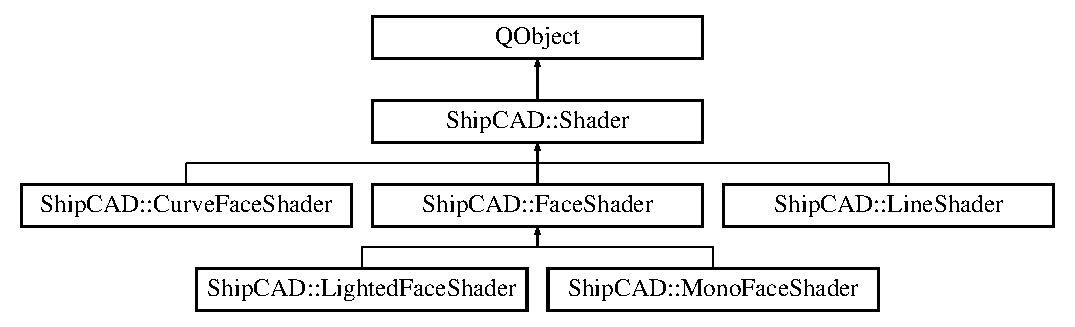
\includegraphics[height=3.950617cm]{classShipCAD_1_1Shader}
\end{center}
\end{figure}
\subsection*{Public Member Functions}
\begin{DoxyCompactItemize}
\item 
\hyperlink{classShipCAD_1_1Shader_a36bc24054e22fb965b04dae9a2b76eb7}{Shader} (\hyperlink{classShipCAD_1_1Viewport}{Viewport} $\ast$vp)
\item 
virtual \hyperlink{classShipCAD_1_1Shader_aff01df87e8a102f270b5b135a295e59d}{$\sim$\+Shader} ()
\item 
virtual void \hyperlink{classShipCAD_1_1Shader_a011fae279e362f548e8c4e4b35b7291e}{initialize} (const char $\ast$vertex\+Shader\+Source, const char $\ast$fragment\+Shader\+Source, std\+::vector$<$ std\+::string $>$ uniforms, std\+::vector$<$ std\+::string $>$ attributes)
\item 
void \hyperlink{classShipCAD_1_1Shader_ac8faec958f9d5806510d39be5f512c8e}{add\+Uniform} (const std\+::string \&name)
\item 
void \hyperlink{classShipCAD_1_1Shader_a6a298be357d7860d859aedbe397b81b9}{add\+Attribute} (const std\+::string \&name)
\item 
void \hyperlink{classShipCAD_1_1Shader_a00c06ead1e413d5d5ecbced82478f753}{bind} ()
\item 
void \hyperlink{classShipCAD_1_1Shader_a0f41d7628964320846101cf5938a928e}{release} ()
\end{DoxyCompactItemize}
\subsection*{Protected Attributes}
\begin{DoxyCompactItemize}
\item 
\hyperlink{classShipCAD_1_1Viewport}{Viewport} $\ast$ \hyperlink{classShipCAD_1_1Shader_a0ee19c28f4fd4260b70095ccd433d546}{\+\_\+viewport}
\item 
Q\+Open\+G\+L\+Shader\+Program $\ast$ \hyperlink{classShipCAD_1_1Shader_a3967404471db3284a2448c4a39b8c230}{\+\_\+program}
\item 
std\+::map$<$ std\+::string, G\+Luint $>$ \hyperlink{classShipCAD_1_1Shader_a5c98e4ae6e3403f179a3fcf204b34baf}{\+\_\+uniforms}
\item 
std\+::map$<$ std\+::string, G\+Luint $>$ \hyperlink{classShipCAD_1_1Shader_af2f710f7b4d792fea09ddd11ab0cdf25}{\+\_\+attributes}
\end{DoxyCompactItemize}


\subsection{Detailed Description}


Definition at line 45 of file shader.\+h.



\subsection{Constructor \& Destructor Documentation}
\index{Ship\+C\+A\+D\+::\+Shader@{Ship\+C\+A\+D\+::\+Shader}!Shader@{Shader}}
\index{Shader@{Shader}!Ship\+C\+A\+D\+::\+Shader@{Ship\+C\+A\+D\+::\+Shader}}
\subsubsection[{\texorpdfstring{Shader(\+Viewport $\ast$vp)}{Shader(Viewport *vp)}}]{\setlength{\rightskip}{0pt plus 5cm}Shader\+::\+Shader (
\begin{DoxyParamCaption}
\item[{{\bf Viewport} $\ast$}]{vp}
\end{DoxyParamCaption}
)\hspace{0.3cm}{\ttfamily [explicit]}}\hypertarget{classShipCAD_1_1Shader_a36bc24054e22fb965b04dae9a2b76eb7}{}\label{classShipCAD_1_1Shader_a36bc24054e22fb965b04dae9a2b76eb7}


Definition at line 42 of file shader.\+cpp.

\index{Ship\+C\+A\+D\+::\+Shader@{Ship\+C\+A\+D\+::\+Shader}!````~Shader@{$\sim$\+Shader}}
\index{````~Shader@{$\sim$\+Shader}!Ship\+C\+A\+D\+::\+Shader@{Ship\+C\+A\+D\+::\+Shader}}
\subsubsection[{\texorpdfstring{$\sim$\+Shader()}{~Shader()}}]{\setlength{\rightskip}{0pt plus 5cm}Shader\+::$\sim$\+Shader (
\begin{DoxyParamCaption}
{}
\end{DoxyParamCaption}
)\hspace{0.3cm}{\ttfamily [virtual]}}\hypertarget{classShipCAD_1_1Shader_aff01df87e8a102f270b5b135a295e59d}{}\label{classShipCAD_1_1Shader_aff01df87e8a102f270b5b135a295e59d}


Definition at line 48 of file shader.\+cpp.



\subsection{Member Function Documentation}
\index{Ship\+C\+A\+D\+::\+Shader@{Ship\+C\+A\+D\+::\+Shader}!add\+Attribute@{add\+Attribute}}
\index{add\+Attribute@{add\+Attribute}!Ship\+C\+A\+D\+::\+Shader@{Ship\+C\+A\+D\+::\+Shader}}
\subsubsection[{\texorpdfstring{add\+Attribute(const std\+::string \&name)}{addAttribute(const std::string &name)}}]{\setlength{\rightskip}{0pt plus 5cm}void Shader\+::add\+Attribute (
\begin{DoxyParamCaption}
\item[{const std\+::string \&}]{name}
\end{DoxyParamCaption}
)}\hypertarget{classShipCAD_1_1Shader_a6a298be357d7860d859aedbe397b81b9}{}\label{classShipCAD_1_1Shader_a6a298be357d7860d859aedbe397b81b9}


Definition at line 81 of file shader.\+cpp.

\index{Ship\+C\+A\+D\+::\+Shader@{Ship\+C\+A\+D\+::\+Shader}!add\+Uniform@{add\+Uniform}}
\index{add\+Uniform@{add\+Uniform}!Ship\+C\+A\+D\+::\+Shader@{Ship\+C\+A\+D\+::\+Shader}}
\subsubsection[{\texorpdfstring{add\+Uniform(const std\+::string \&name)}{addUniform(const std::string &name)}}]{\setlength{\rightskip}{0pt plus 5cm}void Shader\+::add\+Uniform (
\begin{DoxyParamCaption}
\item[{const std\+::string \&}]{name}
\end{DoxyParamCaption}
)}\hypertarget{classShipCAD_1_1Shader_ac8faec958f9d5806510d39be5f512c8e}{}\label{classShipCAD_1_1Shader_ac8faec958f9d5806510d39be5f512c8e}


Definition at line 70 of file shader.\+cpp.

\index{Ship\+C\+A\+D\+::\+Shader@{Ship\+C\+A\+D\+::\+Shader}!bind@{bind}}
\index{bind@{bind}!Ship\+C\+A\+D\+::\+Shader@{Ship\+C\+A\+D\+::\+Shader}}
\subsubsection[{\texorpdfstring{bind()}{bind()}}]{\setlength{\rightskip}{0pt plus 5cm}void Ship\+C\+A\+D\+::\+Shader\+::bind (
\begin{DoxyParamCaption}
{}
\end{DoxyParamCaption}
)\hspace{0.3cm}{\ttfamily [inline]}}\hypertarget{classShipCAD_1_1Shader_a00c06ead1e413d5d5ecbced82478f753}{}\label{classShipCAD_1_1Shader_a00c06ead1e413d5d5ecbced82478f753}


Definition at line 62 of file shader.\+h.

\index{Ship\+C\+A\+D\+::\+Shader@{Ship\+C\+A\+D\+::\+Shader}!initialize@{initialize}}
\index{initialize@{initialize}!Ship\+C\+A\+D\+::\+Shader@{Ship\+C\+A\+D\+::\+Shader}}
\subsubsection[{\texorpdfstring{initialize(const char $\ast$vertex\+Shader\+Source, const char $\ast$fragment\+Shader\+Source, std\+::vector$<$ std\+::string $>$ uniforms, std\+::vector$<$ std\+::string $>$ attributes)}{initialize(const char *vertexShaderSource, const char *fragmentShaderSource, std::vector< std::string > uniforms, std::vector< std::string > attributes)}}]{\setlength{\rightskip}{0pt plus 5cm}void Shader\+::initialize (
\begin{DoxyParamCaption}
\item[{const char $\ast$}]{vertex\+Shader\+Source, }
\item[{const char $\ast$}]{fragment\+Shader\+Source, }
\item[{std\+::vector$<$ std\+::string $>$}]{uniforms, }
\item[{std\+::vector$<$ std\+::string $>$}]{attributes}
\end{DoxyParamCaption}
)\hspace{0.3cm}{\ttfamily [virtual]}}\hypertarget{classShipCAD_1_1Shader_a011fae279e362f548e8c4e4b35b7291e}{}\label{classShipCAD_1_1Shader_a011fae279e362f548e8c4e4b35b7291e}


Definition at line 53 of file shader.\+cpp.

\index{Ship\+C\+A\+D\+::\+Shader@{Ship\+C\+A\+D\+::\+Shader}!release@{release}}
\index{release@{release}!Ship\+C\+A\+D\+::\+Shader@{Ship\+C\+A\+D\+::\+Shader}}
\subsubsection[{\texorpdfstring{release()}{release()}}]{\setlength{\rightskip}{0pt plus 5cm}void Ship\+C\+A\+D\+::\+Shader\+::release (
\begin{DoxyParamCaption}
{}
\end{DoxyParamCaption}
)\hspace{0.3cm}{\ttfamily [inline]}}\hypertarget{classShipCAD_1_1Shader_a0f41d7628964320846101cf5938a928e}{}\label{classShipCAD_1_1Shader_a0f41d7628964320846101cf5938a928e}


Definition at line 63 of file shader.\+h.



\subsection{Member Data Documentation}
\index{Ship\+C\+A\+D\+::\+Shader@{Ship\+C\+A\+D\+::\+Shader}!\+\_\+attributes@{\+\_\+attributes}}
\index{\+\_\+attributes@{\+\_\+attributes}!Ship\+C\+A\+D\+::\+Shader@{Ship\+C\+A\+D\+::\+Shader}}
\subsubsection[{\texorpdfstring{\+\_\+attributes}{_attributes}}]{\setlength{\rightskip}{0pt plus 5cm}std\+::map$<$std\+::string, G\+Luint$>$ Ship\+C\+A\+D\+::\+Shader\+::\+\_\+attributes\hspace{0.3cm}{\ttfamily [protected]}}\hypertarget{classShipCAD_1_1Shader_af2f710f7b4d792fea09ddd11ab0cdf25}{}\label{classShipCAD_1_1Shader_af2f710f7b4d792fea09ddd11ab0cdf25}


Definition at line 70 of file shader.\+h.

\index{Ship\+C\+A\+D\+::\+Shader@{Ship\+C\+A\+D\+::\+Shader}!\+\_\+program@{\+\_\+program}}
\index{\+\_\+program@{\+\_\+program}!Ship\+C\+A\+D\+::\+Shader@{Ship\+C\+A\+D\+::\+Shader}}
\subsubsection[{\texorpdfstring{\+\_\+program}{_program}}]{\setlength{\rightskip}{0pt plus 5cm}Q\+Open\+G\+L\+Shader\+Program$\ast$ Ship\+C\+A\+D\+::\+Shader\+::\+\_\+program\hspace{0.3cm}{\ttfamily [protected]}}\hypertarget{classShipCAD_1_1Shader_a3967404471db3284a2448c4a39b8c230}{}\label{classShipCAD_1_1Shader_a3967404471db3284a2448c4a39b8c230}


Definition at line 68 of file shader.\+h.

\index{Ship\+C\+A\+D\+::\+Shader@{Ship\+C\+A\+D\+::\+Shader}!\+\_\+uniforms@{\+\_\+uniforms}}
\index{\+\_\+uniforms@{\+\_\+uniforms}!Ship\+C\+A\+D\+::\+Shader@{Ship\+C\+A\+D\+::\+Shader}}
\subsubsection[{\texorpdfstring{\+\_\+uniforms}{_uniforms}}]{\setlength{\rightskip}{0pt plus 5cm}std\+::map$<$std\+::string, G\+Luint$>$ Ship\+C\+A\+D\+::\+Shader\+::\+\_\+uniforms\hspace{0.3cm}{\ttfamily [protected]}}\hypertarget{classShipCAD_1_1Shader_a5c98e4ae6e3403f179a3fcf204b34baf}{}\label{classShipCAD_1_1Shader_a5c98e4ae6e3403f179a3fcf204b34baf}


Definition at line 69 of file shader.\+h.

\index{Ship\+C\+A\+D\+::\+Shader@{Ship\+C\+A\+D\+::\+Shader}!\+\_\+viewport@{\+\_\+viewport}}
\index{\+\_\+viewport@{\+\_\+viewport}!Ship\+C\+A\+D\+::\+Shader@{Ship\+C\+A\+D\+::\+Shader}}
\subsubsection[{\texorpdfstring{\+\_\+viewport}{_viewport}}]{\setlength{\rightskip}{0pt plus 5cm}{\bf Viewport}$\ast$ Ship\+C\+A\+D\+::\+Shader\+::\+\_\+viewport\hspace{0.3cm}{\ttfamily [protected]}}\hypertarget{classShipCAD_1_1Shader_a0ee19c28f4fd4260b70095ccd433d546}{}\label{classShipCAD_1_1Shader_a0ee19c28f4fd4260b70095ccd433d546}


Definition at line 67 of file shader.\+h.



The documentation for this class was generated from the following files\+:\begin{DoxyCompactItemize}
\item 
Ship\+C\+A\+Dlib/\hyperlink{shader_8h}{shader.\+h}\item 
Ship\+C\+A\+Dlib/\hyperlink{shader_8cpp}{shader.\+cpp}\end{DoxyCompactItemize}

\hypertarget{classShipCAD_1_1ShipCADModel}{}\section{Ship\+C\+AD\+:\+:Ship\+C\+A\+D\+Model Class Reference}
\label{classShipCAD_1_1ShipCADModel}\index{Ship\+C\+A\+D\+::\+Ship\+C\+A\+D\+Model@{Ship\+C\+A\+D\+::\+Ship\+C\+A\+D\+Model}}


{\ttfamily \#include $<$shipcadmodel.\+h$>$}

Inheritance diagram for Ship\+C\+AD\+:\+:Ship\+C\+A\+D\+Model\+:\begin{figure}[H]
\begin{center}
\leavevmode
\includegraphics[height=2.000000cm]{classShipCAD_1_1ShipCADModel}
\end{center}
\end{figure}
\subsection*{Signals}
\begin{DoxyCompactItemize}
\item 
void \hyperlink{classShipCAD_1_1ShipCADModel_a036ed7f2f1f5e592c64ef8f0ccf29204}{undo\+Data\+Changed} ()
\end{DoxyCompactItemize}
\subsection*{Public Member Functions}
\begin{DoxyCompactItemize}
\item 
\hyperlink{classShipCAD_1_1ShipCADModel_abede72e53058c2ecf8dc2c4b2a7c8014}{Ship\+C\+A\+D\+Model} ()
\item 
\hyperlink{classShipCAD_1_1ShipCADModel_a9731f3987d1f1d31d9df48f129a65fea}{$\sim$\+Ship\+C\+A\+D\+Model} ()
\item 
\hyperlink{classShipCAD_1_1SubdivisionSurface}{Subdivision\+Surface} $\ast$ \hyperlink{classShipCAD_1_1ShipCADModel_a6941ad7a2b167419e844823fa8461019}{get\+Surface} ()
\item 
const \hyperlink{classShipCAD_1_1SubdivisionSurface}{Subdivision\+Surface} $\ast$ \hyperlink{classShipCAD_1_1ShipCADModel_ab0b738e5f12d8f7046570704fd801cc6}{get\+Surface} () const 
\item 
\hyperlink{classShipCAD_1_1Visibility}{Visibility} \& \hyperlink{classShipCAD_1_1ShipCADModel_a50cca4c783baeba58c8068c9b8a5d6a4}{get\+Visibility} ()
\item 
const \hyperlink{classShipCAD_1_1Visibility}{Visibility} \& \hyperlink{classShipCAD_1_1ShipCADModel_a29d8990bbd06e11c93c6639b76b9fde1}{get\+Visibility} () const 
\item 
\hyperlink{classShipCAD_1_1ProjectSettings}{Project\+Settings} \& \hyperlink{classShipCAD_1_1ShipCADModel_a94a8eed8ac8ff4ad8287a0a1113e3271}{get\+Project\+Settings} ()
\item 
\hyperlink{classShipCAD_1_1Preferences}{Preferences} \& \hyperlink{classShipCAD_1_1ShipCADModel_aa6af8872deba5b401ac575a85901a265}{get\+Preferences} ()
\item 
void \hyperlink{classShipCAD_1_1ShipCADModel_adcf0db573afa7c865de68d0b36d41f15}{new\+Model} (\hyperlink{namespaceShipCAD_ac6a7a28b4b063771afae92decb602da5}{unit\+\_\+type\+\_\+t} units, float length, float breadth, float draft, size\+\_\+t rows, size\+\_\+t cols)
\begin{DoxyCompactList}\small\item\em create a new model \end{DoxyCompactList}\item 
void \hyperlink{classShipCAD_1_1ShipCADModel_a89923c0700e57eebf85332cfc9180765}{build\+Valid\+Frame\+Table} (\hyperlink{namespaceShipCAD_a053b941b2c87049bb9380428d4d5a056}{Spline\+Vector} \&dest, bool close\+\_\+at\+\_\+deck)
\begin{DoxyCompactList}\small\item\em Assembles all stations and builds a 2D bodyplan. \end{DoxyCompactList}\item 
bool \hyperlink{classShipCAD_1_1ShipCADModel_ad2333f42cf37a754f3d29b33466e5cd2}{is\+Build} () const 
\item 
void \hyperlink{classShipCAD_1_1ShipCADModel_ab221977f2a8bd4d51d6ee777be0d7b8a}{set\+Build} (bool set)
\item 
void \hyperlink{classShipCAD_1_1ShipCADModel_a5e9e159fc6c1fcd06cc14005bb0e51c8}{scale\+Model} (const Q\+Vector3D \&scale, bool override\+\_\+lock, bool adjust\+\_\+markers)
\begin{DoxyCompactList}\small\item\em scale the entire model and all associated data such as sttions \end{DoxyCompactList}\item 
void \hyperlink{classShipCAD_1_1ShipCADModel_ac1b60be4b08de357c6a1aa0f8e1c0a9b}{move\+Faces} (std\+::vector$<$ \hyperlink{classShipCAD_1_1SubdivisionControlPoint}{Subdivision\+Control\+Point} $\ast$ $>$ \&points, const Q\+Vector3D \&vec, bool adjust\+\_\+markers)
\begin{DoxyCompactList}\small\item\em move selected faces and all associated data \end{DoxyCompactList}\item 
\hyperlink{classShipCAD_1_1Intersection}{Intersection} $\ast$ \hyperlink{classShipCAD_1_1ShipCADModel_a83e2091e476b3ea89c75ecb25f46268b}{create\+Intersection} (\hyperlink{namespaceShipCAD_aa56834b730aafdf2786ddc9a60a046fd}{intersection\+\_\+type\+\_\+t} ty, float distance)
\begin{DoxyCompactList}\small\item\em create an intersection \end{DoxyCompactList}\item 
\hyperlink{classShipCAD_1_1SubdivisionControlPoint}{Subdivision\+Control\+Point} $\ast$ \hyperlink{classShipCAD_1_1ShipCADModel_afe13cf557e067ae883433aa6f5afaf6a}{get\+Active\+Control\+Point} () const 
\begin{DoxyCompactList}\small\item\em get the active control point \end{DoxyCompactList}\item 
void \hyperlink{classShipCAD_1_1ShipCADModel_a523a7e9948d95a71e9008d386daeafee}{set\+Active\+Control\+Point} (\hyperlink{classShipCAD_1_1SubdivisionControlPoint}{Subdivision\+Control\+Point} $\ast$pt)
\begin{DoxyCompactList}\small\item\em set the active control point \end{DoxyCompactList}\item 
\hyperlink{namespaceShipCAD_ae13c7e36dfb1e2300741a631041cd915}{precision\+\_\+t} \hyperlink{classShipCAD_1_1ShipCADModel_a0835431712a18b9f83e64135486c1403}{get\+Precision} () const 
\begin{DoxyCompactList}\small\item\em get precision of model \end{DoxyCompactList}\item 
void \hyperlink{classShipCAD_1_1ShipCADModel_a6133fe12cd13b6ce24424e19a8b1e433}{set\+Precision} (\hyperlink{namespaceShipCAD_ae13c7e36dfb1e2300741a631041cd915}{precision\+\_\+t} precision)
\begin{DoxyCompactList}\small\item\em set precision of model \end{DoxyCompactList}\item 
\hyperlink{namespaceShipCAD_af3a6fa23a7318acbda7b0066b53d694f}{version\+\_\+t} \hyperlink{classShipCAD_1_1ShipCADModel_a837f41ecb002cd0e197d365edbef3d52}{get\+File\+Version} () const 
\item 
void \hyperlink{classShipCAD_1_1ShipCADModel_a44ac7a48c0c01cae73bf723120071e72}{set\+File\+Version} (\hyperlink{namespaceShipCAD_af3a6fa23a7318acbda7b0066b53d694f}{version\+\_\+t} v)
\item 
\hyperlink{namespaceShipCAD_a9910f0963197f9df6125398efd4fa139}{Intersection\+Vector} \& \hyperlink{classShipCAD_1_1ShipCADModel_a86da3ca66e90403ead21ccc67f584c52}{get\+Stations} ()
\item 
\hyperlink{namespaceShipCAD_a9910f0963197f9df6125398efd4fa139}{Intersection\+Vector} \& \hyperlink{classShipCAD_1_1ShipCADModel_a6c147a75fa02e43145de346efb9542fd}{get\+Waterlines} ()
\item 
\hyperlink{namespaceShipCAD_a9910f0963197f9df6125398efd4fa139}{Intersection\+Vector} \& \hyperlink{classShipCAD_1_1ShipCADModel_a8908d7adff0b1aa1ed118103c02c5402}{get\+Buttocks} ()
\item 
\hyperlink{namespaceShipCAD_a9910f0963197f9df6125398efd4fa139}{Intersection\+Vector} \& \hyperlink{classShipCAD_1_1ShipCADModel_a19864f7628c596553f7c89247715b10a}{get\+Diagonals} ()
\item 
\hyperlink{namespaceShipCAD_a66144e3f3a53da01f51c9bdb94fcae31}{edit\+\_\+mode\+\_\+t} \hyperlink{classShipCAD_1_1ShipCADModel_a636a331e17c59db296527d1aca0ad01d}{get\+Edit\+Mode} () const 
\item 
void \hyperlink{classShipCAD_1_1ShipCADModel_a2636160d900b8d8b00802ae78ee87925}{set\+Edit\+Mode} (\hyperlink{namespaceShipCAD_a66144e3f3a53da01f51c9bdb94fcae31}{edit\+\_\+mode\+\_\+t} mode)
\item 
size\+\_\+t \hyperlink{classShipCAD_1_1ShipCADModel_a859625224375157010421a69f96ec639}{count\+Selected\+Items} () const 
\begin{DoxyCompactList}\small\item\em count the number of currently selected items \end{DoxyCompactList}\item 
void \hyperlink{classShipCAD_1_1ShipCADModel_a690bd5621d82d15a28ea59c09ded99d8}{clear\+Selected\+Items} ()
\begin{DoxyCompactList}\small\item\em clear all selected items \end{DoxyCompactList}\item 
Q\+String \hyperlink{classShipCAD_1_1ShipCADModel_a4c29a9dd9e31c652a82b6398c8f7b983}{get\+Filename} () const 
\begin{DoxyCompactList}\small\item\em name of file \end{DoxyCompactList}\item 
void \hyperlink{classShipCAD_1_1ShipCADModel_a07daf75d876f80296f841f5c8d2327cb}{set\+Filename} (const Q\+String \&name)
\begin{DoxyCompactList}\small\item\em set the name of the file \end{DoxyCompactList}\item 
bool \hyperlink{classShipCAD_1_1ShipCADModel_a9aa140f98f5f02a30743e2b9ce3d7d28}{is\+Filename\+Set} () const 
\begin{DoxyCompactList}\small\item\em get flag for filename set \end{DoxyCompactList}\item 
void \hyperlink{classShipCAD_1_1ShipCADModel_a960f3e97ef2aa847c9bb7cdc7731cd39}{set\+Filename\+Set} (bool flag)
\begin{DoxyCompactList}\small\item\em set flag for filename set \end{DoxyCompactList}\item 
\hyperlink{namespaceShipCAD_a0c7b012d8868cbb43871cf0bf303ccc6}{Hydrostatic\+Calc\+Vector} \& \hyperlink{classShipCAD_1_1ShipCADModel_aafc30dd7d6b9db4ccfc7bf1c4e2b3b11}{get\+Hydrostatic\+Calculations} ()
\item 
\hyperlink{namespaceShipCAD_a36fff5b53986f6d6976afc749463ef22}{Marker\+Vector} \& \hyperlink{classShipCAD_1_1ShipCADModel_abc5faaa00b4b34bc1b0b1cd52af4ab3b}{get\+Markers} ()
\item 
size\+\_\+t \hyperlink{classShipCAD_1_1ShipCADModel_a6feda4dd07262d1f137f8f8a677bd23d}{number\+Of\+Markers} () const 
\item 
\hyperlink{classShipCAD_1_1Marker}{Marker} $\ast$ \hyperlink{classShipCAD_1_1ShipCADModel_ac7fd2d6607f589a20444f3efb8fde63b}{add\+Marker} ()
\item 
bool \hyperlink{classShipCAD_1_1ShipCADModel_ac7aabd58923105ec36b27d44d747aa42}{is\+Selected\+Marker} (\hyperlink{classShipCAD_1_1Marker}{Marker} $\ast$mark) const 
\item 
void \hyperlink{classShipCAD_1_1ShipCADModel_afd7e984f4070d08cb16264c1b731580f}{set\+Selected\+Marker} (\hyperlink{classShipCAD_1_1Marker}{Marker} $\ast$mark)
\item 
void \hyperlink{classShipCAD_1_1ShipCADModel_a7fb06b0a1fa75ef02597752fc3f691a2}{remove\+Selected\+Marker} (\hyperlink{classShipCAD_1_1Marker}{Marker} $\ast$mark)
\item 
size\+\_\+t \hyperlink{classShipCAD_1_1ShipCADModel_a3138ff1240e6ccc1e9072c066a0ffedf}{number\+Of\+Selected\+Markers} () const 
\item 
void \hyperlink{classShipCAD_1_1ShipCADModel_a2e6888d7b5e8d6346286d0262a93a183}{delete\+Marker} (\hyperlink{classShipCAD_1_1Marker}{Marker} $\ast$mark)
\item 
\hyperlink{classShipCAD_1_1Flowline}{Flowline} $\ast$ \hyperlink{classShipCAD_1_1ShipCADModel_a73494d53c57b4401f59f3feb3d73941b}{add\+Flowline} (const Q\+Vector2D \&pt, \hyperlink{namespaceShipCAD_aeeeb05810f2e31ef89fd4ac6b6ba9c0a}{viewport\+\_\+type\+\_\+t} ty)
\item 
\hyperlink{classShipCAD_1_1Flowline}{Flowline} $\ast$ \hyperlink{classShipCAD_1_1ShipCADModel_afc5654f671a17dd6672230648842975e}{get\+Flowline} (size\+\_\+t index)
\item 
size\+\_\+t \hyperlink{classShipCAD_1_1ShipCADModel_a7bb6418bfa20645211e6bdbf8c6ef951}{number\+Of\+Flowlines} () const 
\item 
bool \hyperlink{classShipCAD_1_1ShipCADModel_afcac043bc1d1c627e95ca1bc4aa0174e}{is\+Selected\+Flowline} (\hyperlink{classShipCAD_1_1Flowline}{Flowline} $\ast$flow) const 
\begin{DoxyCompactList}\small\item\em is the flowline selected \end{DoxyCompactList}\item 
void \hyperlink{classShipCAD_1_1ShipCADModel_a33962f53b44136c2840f8f7fa2e362f3}{set\+Selected\+Flowline} (\hyperlink{classShipCAD_1_1Flowline}{Flowline} $\ast$flow)
\begin{DoxyCompactList}\small\item\em set a flowline as selected \end{DoxyCompactList}\item 
void \hyperlink{classShipCAD_1_1ShipCADModel_a341f8be57a7cf6c04356a731b3b30c37}{remove\+Selected\+Flowline} (\hyperlink{classShipCAD_1_1Flowline}{Flowline} $\ast$flow)
\begin{DoxyCompactList}\small\item\em deselect a flowline \end{DoxyCompactList}\item 
size\+\_\+t \hyperlink{classShipCAD_1_1ShipCADModel_a4c534c40efab65e1b92481f1fa7f07a9}{number\+Of\+Selected\+Flowlines} () const 
\begin{DoxyCompactList}\small\item\em count of selected flowlines \end{DoxyCompactList}\item 
void \hyperlink{classShipCAD_1_1ShipCADModel_a7777da02744250aebce9be35063ba0f5}{delete\+Flowline} (\hyperlink{classShipCAD_1_1Flowline}{Flowline} $\ast$flow)
\begin{DoxyCompactList}\small\item\em delete a flowline from the model \end{DoxyCompactList}\item 
bool \hyperlink{classShipCAD_1_1ShipCADModel_aac25049d627953c15c5343b2f888f688}{is\+File\+Changed} () const 
\begin{DoxyCompactList}\small\item\em file changed flag \end{DoxyCompactList}\item 
void \hyperlink{classShipCAD_1_1ShipCADModel_ae8fe6d69df313f7459235de1a0614e8c}{set\+File\+Changed} (bool changed)
\begin{DoxyCompactList}\small\item\em set file changed flag \end{DoxyCompactList}\item 
\hyperlink{classShipCAD_1_1UndoObject}{Undo\+Object} $\ast$ \hyperlink{classShipCAD_1_1ShipCADModel_a0e9a74dd26baa734437aba2ee05fa940}{create\+Undo} (const Q\+String \&undotext, bool accept)
\begin{DoxyCompactList}\small\item\em create an undo object \end{DoxyCompactList}\item 
void \hyperlink{classShipCAD_1_1ShipCADModel_a7e54e8d3a1b972014a3cd71cc57c74dc}{accept\+Undo} (\hyperlink{classShipCAD_1_1UndoObject}{Undo\+Object} $\ast$\hyperlink{classShipCAD_1_1ShipCADModel_a31cd6dcb665c21c1626599d57ae73684}{undo})
\begin{DoxyCompactList}\small\item\em add an undo to the undo list \end{DoxyCompactList}\item 
void \hyperlink{classShipCAD_1_1ShipCADModel_a31cd6dcb665c21c1626599d57ae73684}{undo} ()
\begin{DoxyCompactList}\small\item\em undo the last operation \end{DoxyCompactList}\item 
void \hyperlink{classShipCAD_1_1ShipCADModel_ac7f369ecf1a53a751f8774263d3ecd95}{redo} ()
\begin{DoxyCompactList}\small\item\em redo the last undo \end{DoxyCompactList}\item 
size\+\_\+t \hyperlink{classShipCAD_1_1ShipCADModel_a6fc43771e5ab6fe985ed894f4a1f779c}{get\+Undo\+Memory} () const 
\begin{DoxyCompactList}\small\item\em get amount of memory used for undo \end{DoxyCompactList}\item 
bool \hyperlink{classShipCAD_1_1ShipCADModel_a31d65b98d41ec379ae9f27b7cf66b079}{can\+Undo} () const 
\item 
bool \hyperlink{classShipCAD_1_1ShipCADModel_a1178d14769f22603340413c416d6631f}{can\+Redo} () const 
\item 
void \hyperlink{classShipCAD_1_1ShipCADModel_ac8a3a46ed5864f651495bd450d11ef2a}{clear\+Undo} ()
\item 
float \hyperlink{classShipCAD_1_1ShipCADModel_ab16487a794947608cace81a06552b2b1}{find\+Lowest\+Hydrostatics\+Point} () const 
\begin{DoxyCompactList}\small\item\em get the lowest underwater point of hull \end{DoxyCompactList}\item 
void \hyperlink{classShipCAD_1_1ShipCADModel_ad3e49bc04c73dc221e48d15974b68f41}{load\+Binary} (\hyperlink{classShipCAD_1_1FileBuffer}{File\+Buffer} \&source)
\item 
void \hyperlink{classShipCAD_1_1ShipCADModel_a64c7c4ddffffdd1be2f27eb4210af2b7}{save\+Binary} (\hyperlink{classShipCAD_1_1FileBuffer}{File\+Buffer} \&dest)
\item 
void \hyperlink{classShipCAD_1_1ShipCADModel_a6be8a5765b6b9ee5b5dc0397bdd43be5}{load\+Preview} (\hyperlink{classShipCAD_1_1FileBuffer}{File\+Buffer} \&source, Q\+Image $\ast$image)
\begin{DoxyCompactList}\small\item\em load the preview image from a file \end{DoxyCompactList}\item 
void \hyperlink{classShipCAD_1_1ShipCADModel_a0d969a8b0f05767d6507290f118d769c}{save\+Part} (const Q\+String \&filename, \hyperlink{classShipCAD_1_1FileBuffer}{File\+Buffer} \&buffer, std\+::vector$<$ \hyperlink{classShipCAD_1_1SubdivisionControlFace}{Subdivision\+Control\+Face} $\ast$ $>$ \&faces)
\begin{DoxyCompactList}\small\item\em save selected faces as a part file \end{DoxyCompactList}\item 
bool \hyperlink{classShipCAD_1_1ShipCADModel_a167bdeeb8995f102acdbb8cdb92f34e3}{load\+Part} (\hyperlink{classShipCAD_1_1FileBuffer}{File\+Buffer} \&source, \hyperlink{namespaceShipCAD_af3a6fa23a7318acbda7b0066b53d694f}{version\+\_\+t} \&partversion)
\begin{DoxyCompactList}\small\item\em load a part \end{DoxyCompactList}\item 
void \hyperlink{classShipCAD_1_1ShipCADModel_ae03a368cf40f1781fb0ed8a60248dcc6}{load\+Chines\+From\+Text} (Q\+Text\+Stream \&file, \hyperlink{namespaceShipCAD_a053b941b2c87049bb9380428d4d5a056}{Spline\+Vector} \&splines)
\begin{DoxyCompactList}\small\item\em load splines from a text file \end{DoxyCompactList}\item 
void \hyperlink{classShipCAD_1_1ShipCADModel_a860a91c09307c71f738a75aec159e6d0}{import\+Chines} (size\+\_\+t np, \hyperlink{namespaceShipCAD_a053b941b2c87049bb9380428d4d5a056}{Spline\+Vector} \&chines)
\begin{DoxyCompactList}\small\item\em imports chines and creates developable surface \end{DoxyCompactList}\item 
void \hyperlink{classShipCAD_1_1ShipCADModel_a1b27573aab3a458f9002a7e4e327736a}{rebuild\+Model} (bool redo\+\_\+intersections)
\item 
void \hyperlink{classShipCAD_1_1ShipCADModel_aa7d2417dcc847ccf0f72d57eb333410e}{draw\+With\+Painter} (\hyperlink{classShipCAD_1_1Viewport}{Viewport} \&vp, Q\+Painter $\ast$painter)
\item 
void \hyperlink{classShipCAD_1_1ShipCADModel_abf593b803e96a1fd8e56f36b3b6d0954}{draw} (\hyperlink{classShipCAD_1_1Viewport}{Viewport} \&vp)
\item 
void \hyperlink{classShipCAD_1_1ShipCADModel_a83dbf01267c7736a8676336785178db6}{delete\+Selected} ()
\begin{DoxyCompactList}\small\item\em delete all selected items \end{DoxyCompactList}\item 
void \hyperlink{classShipCAD_1_1ShipCADModel_ad2f9dfd32667e9ac690de184b7e576f1}{clear} ()
\item 
void \hyperlink{classShipCAD_1_1ShipCADModel_a7ab84a738b747c4fcb2c3627e56d4bd0}{extents} (Q\+Vector3D \&min, Q\+Vector3D \&max)
\begin{DoxyCompactList}\small\item\em find the bounding box of the model \end{DoxyCompactList}\end{DoxyCompactItemize}
\subsection*{Protected Member Functions}
\begin{DoxyCompactItemize}
\item 
void \hyperlink{classShipCAD_1_1ShipCADModel_af719e24c12a21220c105fc7510d7b8ad}{draw\+Grid} (\hyperlink{classShipCAD_1_1Viewport}{Viewport} \&vp, Q\+Painter $\ast$painter)
\item 
\hyperlink{classShipCAD_1_1UndoObject}{Undo\+Object} $\ast$ \hyperlink{classShipCAD_1_1ShipCADModel_aa8079da42c7e5ab56ff60af82432d29d}{create\+Redo} ()
\begin{DoxyCompactList}\small\item\em create temp redo object at end of undo list \end{DoxyCompactList}\end{DoxyCompactItemize}


\subsection{Detailed Description}


Definition at line 63 of file shipcadmodel.\+h.



\subsection{Constructor \& Destructor Documentation}
\index{Ship\+C\+A\+D\+::\+Ship\+C\+A\+D\+Model@{Ship\+C\+A\+D\+::\+Ship\+C\+A\+D\+Model}!Ship\+C\+A\+D\+Model@{Ship\+C\+A\+D\+Model}}
\index{Ship\+C\+A\+D\+Model@{Ship\+C\+A\+D\+Model}!Ship\+C\+A\+D\+::\+Ship\+C\+A\+D\+Model@{Ship\+C\+A\+D\+::\+Ship\+C\+A\+D\+Model}}
\subsubsection[{\texorpdfstring{Ship\+C\+A\+D\+Model()}{ShipCADModel()}}]{\setlength{\rightskip}{0pt plus 5cm}Ship\+C\+A\+D\+Model\+::\+Ship\+C\+A\+D\+Model (
\begin{DoxyParamCaption}
{}
\end{DoxyParamCaption}
)\hspace{0.3cm}{\ttfamily [explicit]}}\hypertarget{classShipCAD_1_1ShipCADModel_abede72e53058c2ecf8dc2c4b2a7c8014}{}\label{classShipCAD_1_1ShipCADModel_abede72e53058c2ecf8dc2c4b2a7c8014}


Definition at line 53 of file shipcadmodel.\+cpp.

\index{Ship\+C\+A\+D\+::\+Ship\+C\+A\+D\+Model@{Ship\+C\+A\+D\+::\+Ship\+C\+A\+D\+Model}!````~Ship\+C\+A\+D\+Model@{$\sim$\+Ship\+C\+A\+D\+Model}}
\index{````~Ship\+C\+A\+D\+Model@{$\sim$\+Ship\+C\+A\+D\+Model}!Ship\+C\+A\+D\+::\+Ship\+C\+A\+D\+Model@{Ship\+C\+A\+D\+::\+Ship\+C\+A\+D\+Model}}
\subsubsection[{\texorpdfstring{$\sim$\+Ship\+C\+A\+D\+Model()}{~ShipCADModel()}}]{\setlength{\rightskip}{0pt plus 5cm}Ship\+C\+A\+D\+::\+Ship\+C\+A\+D\+Model\+::$\sim$\+Ship\+C\+A\+D\+Model (
\begin{DoxyParamCaption}
{}
\end{DoxyParamCaption}
)\hspace{0.3cm}{\ttfamily [inline]}}\hypertarget{classShipCAD_1_1ShipCADModel_a9731f3987d1f1d31d9df48f129a65fea}{}\label{classShipCAD_1_1ShipCADModel_a9731f3987d1f1d31d9df48f129a65fea}


Definition at line 69 of file shipcadmodel.\+h.



\subsection{Member Function Documentation}
\index{Ship\+C\+A\+D\+::\+Ship\+C\+A\+D\+Model@{Ship\+C\+A\+D\+::\+Ship\+C\+A\+D\+Model}!accept\+Undo@{accept\+Undo}}
\index{accept\+Undo@{accept\+Undo}!Ship\+C\+A\+D\+::\+Ship\+C\+A\+D\+Model@{Ship\+C\+A\+D\+::\+Ship\+C\+A\+D\+Model}}
\subsubsection[{\texorpdfstring{accept\+Undo(\+Undo\+Object $\ast$undo)}{acceptUndo(UndoObject *undo)}}]{\setlength{\rightskip}{0pt plus 5cm}void Ship\+C\+A\+D\+Model\+::accept\+Undo (
\begin{DoxyParamCaption}
\item[{{\bf Undo\+Object} $\ast$}]{undo}
\end{DoxyParamCaption}
)}\hypertarget{classShipCAD_1_1ShipCADModel_a7e54e8d3a1b972014a3cd71cc57c74dc}{}\label{classShipCAD_1_1ShipCADModel_a7e54e8d3a1b972014a3cd71cc57c74dc}


add an undo to the undo list 


\begin{DoxyParams}{Parameters}
{\em undo} & the object to put in the undo list \\
\hline
\end{DoxyParams}


Definition at line 351 of file shipcadmodel.\+cpp.

\index{Ship\+C\+A\+D\+::\+Ship\+C\+A\+D\+Model@{Ship\+C\+A\+D\+::\+Ship\+C\+A\+D\+Model}!add\+Flowline@{add\+Flowline}}
\index{add\+Flowline@{add\+Flowline}!Ship\+C\+A\+D\+::\+Ship\+C\+A\+D\+Model@{Ship\+C\+A\+D\+::\+Ship\+C\+A\+D\+Model}}
\subsubsection[{\texorpdfstring{add\+Flowline(const Q\+Vector2\+D \&pt, viewport\+\_\+type\+\_\+t ty)}{addFlowline(const QVector2D &pt, viewport_type_t ty)}}]{\setlength{\rightskip}{0pt plus 5cm}{\bf Flowline} $\ast$ Ship\+C\+A\+D\+Model\+::add\+Flowline (
\begin{DoxyParamCaption}
\item[{const Q\+Vector2D \&}]{pt, }
\item[{{\bf viewport\+\_\+type\+\_\+t}}]{ty}
\end{DoxyParamCaption}
)}\hypertarget{classShipCAD_1_1ShipCADModel_a73494d53c57b4401f59f3feb3d73941b}{}\label{classShipCAD_1_1ShipCADModel_a73494d53c57b4401f59f3feb3d73941b}


Definition at line 1127 of file shipcadmodel.\+cpp.

\index{Ship\+C\+A\+D\+::\+Ship\+C\+A\+D\+Model@{Ship\+C\+A\+D\+::\+Ship\+C\+A\+D\+Model}!add\+Marker@{add\+Marker}}
\index{add\+Marker@{add\+Marker}!Ship\+C\+A\+D\+::\+Ship\+C\+A\+D\+Model@{Ship\+C\+A\+D\+::\+Ship\+C\+A\+D\+Model}}
\subsubsection[{\texorpdfstring{add\+Marker()}{addMarker()}}]{\setlength{\rightskip}{0pt plus 5cm}{\bf Marker} $\ast$ Ship\+C\+A\+D\+Model\+::add\+Marker (
\begin{DoxyParamCaption}
{}
\end{DoxyParamCaption}
)}\hypertarget{classShipCAD_1_1ShipCADModel_ac7fd2d6607f589a20444f3efb8fde63b}{}\label{classShipCAD_1_1ShipCADModel_ac7fd2d6607f589a20444f3efb8fde63b}


Definition at line 1114 of file shipcadmodel.\+cpp.

\index{Ship\+C\+A\+D\+::\+Ship\+C\+A\+D\+Model@{Ship\+C\+A\+D\+::\+Ship\+C\+A\+D\+Model}!build\+Valid\+Frame\+Table@{build\+Valid\+Frame\+Table}}
\index{build\+Valid\+Frame\+Table@{build\+Valid\+Frame\+Table}!Ship\+C\+A\+D\+::\+Ship\+C\+A\+D\+Model@{Ship\+C\+A\+D\+::\+Ship\+C\+A\+D\+Model}}
\subsubsection[{\texorpdfstring{build\+Valid\+Frame\+Table(\+Spline\+Vector \&dest, bool close\+\_\+at\+\_\+deck)}{buildValidFrameTable(SplineVector &dest, bool close_at_deck)}}]{\setlength{\rightskip}{0pt plus 5cm}void Ship\+C\+A\+D\+Model\+::build\+Valid\+Frame\+Table (
\begin{DoxyParamCaption}
\item[{{\bf Spline\+Vector} \&}]{dest, }
\item[{bool}]{close\+\_\+at\+\_\+deck}
\end{DoxyParamCaption}
)}\hypertarget{classShipCAD_1_1ShipCADModel_a89923c0700e57eebf85332cfc9180765}{}\label{classShipCAD_1_1ShipCADModel_a89923c0700e57eebf85332cfc9180765}


Assembles all stations and builds a 2D bodyplan. 


\begin{DoxyParams}{Parameters}
{\em dest} & the spline list with assembled stations \\
\hline
{\em close\+\_\+at\+\_\+deck} & \\
\hline
\end{DoxyParams}


Definition at line 91 of file shipcadmodel.\+cpp.

\index{Ship\+C\+A\+D\+::\+Ship\+C\+A\+D\+Model@{Ship\+C\+A\+D\+::\+Ship\+C\+A\+D\+Model}!can\+Redo@{can\+Redo}}
\index{can\+Redo@{can\+Redo}!Ship\+C\+A\+D\+::\+Ship\+C\+A\+D\+Model@{Ship\+C\+A\+D\+::\+Ship\+C\+A\+D\+Model}}
\subsubsection[{\texorpdfstring{can\+Redo() const }{canRedo() const }}]{\setlength{\rightskip}{0pt plus 5cm}bool Ship\+C\+A\+D\+Model\+::can\+Redo (
\begin{DoxyParamCaption}
{}
\end{DoxyParamCaption}
) const}\hypertarget{classShipCAD_1_1ShipCADModel_a1178d14769f22603340413c416d6631f}{}\label{classShipCAD_1_1ShipCADModel_a1178d14769f22603340413c416d6631f}


Definition at line 447 of file shipcadmodel.\+cpp.

\index{Ship\+C\+A\+D\+::\+Ship\+C\+A\+D\+Model@{Ship\+C\+A\+D\+::\+Ship\+C\+A\+D\+Model}!can\+Undo@{can\+Undo}}
\index{can\+Undo@{can\+Undo}!Ship\+C\+A\+D\+::\+Ship\+C\+A\+D\+Model@{Ship\+C\+A\+D\+::\+Ship\+C\+A\+D\+Model}}
\subsubsection[{\texorpdfstring{can\+Undo() const }{canUndo() const }}]{\setlength{\rightskip}{0pt plus 5cm}bool Ship\+C\+A\+D\+Model\+::can\+Undo (
\begin{DoxyParamCaption}
{}
\end{DoxyParamCaption}
) const}\hypertarget{classShipCAD_1_1ShipCADModel_a31d65b98d41ec379ae9f27b7cf66b079}{}\label{classShipCAD_1_1ShipCADModel_a31d65b98d41ec379ae9f27b7cf66b079}


Definition at line 442 of file shipcadmodel.\+cpp.

\index{Ship\+C\+A\+D\+::\+Ship\+C\+A\+D\+Model@{Ship\+C\+A\+D\+::\+Ship\+C\+A\+D\+Model}!clear@{clear}}
\index{clear@{clear}!Ship\+C\+A\+D\+::\+Ship\+C\+A\+D\+Model@{Ship\+C\+A\+D\+::\+Ship\+C\+A\+D\+Model}}
\subsubsection[{\texorpdfstring{clear()}{clear()}}]{\setlength{\rightskip}{0pt plus 5cm}void Ship\+C\+A\+D\+Model\+::clear (
\begin{DoxyParamCaption}
{}
\end{DoxyParamCaption}
)}\hypertarget{classShipCAD_1_1ShipCADModel_ad2f9dfd32667e9ac690de184b7e576f1}{}\label{classShipCAD_1_1ShipCADModel_ad2f9dfd32667e9ac690de184b7e576f1}


Definition at line 66 of file shipcadmodel.\+cpp.

\index{Ship\+C\+A\+D\+::\+Ship\+C\+A\+D\+Model@{Ship\+C\+A\+D\+::\+Ship\+C\+A\+D\+Model}!clear\+Selected\+Items@{clear\+Selected\+Items}}
\index{clear\+Selected\+Items@{clear\+Selected\+Items}!Ship\+C\+A\+D\+::\+Ship\+C\+A\+D\+Model@{Ship\+C\+A\+D\+::\+Ship\+C\+A\+D\+Model}}
\subsubsection[{\texorpdfstring{clear\+Selected\+Items()}{clearSelectedItems()}}]{\setlength{\rightskip}{0pt plus 5cm}void Ship\+C\+A\+D\+Model\+::clear\+Selected\+Items (
\begin{DoxyParamCaption}
{}
\end{DoxyParamCaption}
)}\hypertarget{classShipCAD_1_1ShipCADModel_a690bd5621d82d15a28ea59c09ded99d8}{}\label{classShipCAD_1_1ShipCADModel_a690bd5621d82d15a28ea59c09ded99d8}


clear all selected items 



Definition at line 252 of file shipcadmodel.\+cpp.

\index{Ship\+C\+A\+D\+::\+Ship\+C\+A\+D\+Model@{Ship\+C\+A\+D\+::\+Ship\+C\+A\+D\+Model}!clear\+Undo@{clear\+Undo}}
\index{clear\+Undo@{clear\+Undo}!Ship\+C\+A\+D\+::\+Ship\+C\+A\+D\+Model@{Ship\+C\+A\+D\+::\+Ship\+C\+A\+D\+Model}}
\subsubsection[{\texorpdfstring{clear\+Undo()}{clearUndo()}}]{\setlength{\rightskip}{0pt plus 5cm}void Ship\+C\+A\+D\+Model\+::clear\+Undo (
\begin{DoxyParamCaption}
{}
\end{DoxyParamCaption}
)}\hypertarget{classShipCAD_1_1ShipCADModel_ac8a3a46ed5864f651495bd450d11ef2a}{}\label{classShipCAD_1_1ShipCADModel_ac8a3a46ed5864f651495bd450d11ef2a}


Definition at line 452 of file shipcadmodel.\+cpp.

\index{Ship\+C\+A\+D\+::\+Ship\+C\+A\+D\+Model@{Ship\+C\+A\+D\+::\+Ship\+C\+A\+D\+Model}!count\+Selected\+Items@{count\+Selected\+Items}}
\index{count\+Selected\+Items@{count\+Selected\+Items}!Ship\+C\+A\+D\+::\+Ship\+C\+A\+D\+Model@{Ship\+C\+A\+D\+::\+Ship\+C\+A\+D\+Model}}
\subsubsection[{\texorpdfstring{count\+Selected\+Items() const }{countSelectedItems() const }}]{\setlength{\rightskip}{0pt plus 5cm}size\+\_\+t Ship\+C\+A\+D\+Model\+::count\+Selected\+Items (
\begin{DoxyParamCaption}
{}
\end{DoxyParamCaption}
) const}\hypertarget{classShipCAD_1_1ShipCADModel_a859625224375157010421a69f96ec639}{}\label{classShipCAD_1_1ShipCADModel_a859625224375157010421a69f96ec639}


count the number of currently selected items 

\begin{DoxyReturn}{Returns}
number of selected items 
\end{DoxyReturn}


Definition at line 239 of file shipcadmodel.\+cpp.

\index{Ship\+C\+A\+D\+::\+Ship\+C\+A\+D\+Model@{Ship\+C\+A\+D\+::\+Ship\+C\+A\+D\+Model}!create\+Intersection@{create\+Intersection}}
\index{create\+Intersection@{create\+Intersection}!Ship\+C\+A\+D\+::\+Ship\+C\+A\+D\+Model@{Ship\+C\+A\+D\+::\+Ship\+C\+A\+D\+Model}}
\subsubsection[{\texorpdfstring{create\+Intersection(intersection\+\_\+type\+\_\+t ty, float distance)}{createIntersection(intersection_type_t ty, float distance)}}]{\setlength{\rightskip}{0pt plus 5cm}{\bf Intersection} $\ast$ Ship\+C\+A\+D\+Model\+::create\+Intersection (
\begin{DoxyParamCaption}
\item[{{\bf intersection\+\_\+type\+\_\+t}}]{ty, }
\item[{float}]{distance}
\end{DoxyParamCaption}
)}\hypertarget{classShipCAD_1_1ShipCADModel_a83e2091e476b3ea89c75ecb25f46268b}{}\label{classShipCAD_1_1ShipCADModel_a83e2091e476b3ea89c75ecb25f46268b}


create an intersection 


\begin{DoxyParams}{Parameters}
{\em type} & which type of intersection \\
\hline
{\em distance} & location of intersection \\
\hline
\end{DoxyParams}
\begin{DoxyReturn}{Returns}
the created intersection, or 0 if not created 
\end{DoxyReturn}


Definition at line 846 of file shipcadmodel.\+cpp.

\index{Ship\+C\+A\+D\+::\+Ship\+C\+A\+D\+Model@{Ship\+C\+A\+D\+::\+Ship\+C\+A\+D\+Model}!create\+Redo@{create\+Redo}}
\index{create\+Redo@{create\+Redo}!Ship\+C\+A\+D\+::\+Ship\+C\+A\+D\+Model@{Ship\+C\+A\+D\+::\+Ship\+C\+A\+D\+Model}}
\subsubsection[{\texorpdfstring{create\+Redo()}{createRedo()}}]{\setlength{\rightskip}{0pt plus 5cm}{\bf Undo\+Object} $\ast$ Ship\+C\+A\+D\+Model\+::create\+Redo (
\begin{DoxyParamCaption}
{}
\end{DoxyParamCaption}
)\hspace{0.3cm}{\ttfamily [protected]}}\hypertarget{classShipCAD_1_1ShipCADModel_aa8079da42c7e5ab56ff60af82432d29d}{}\label{classShipCAD_1_1ShipCADModel_aa8079da42c7e5ab56ff60af82432d29d}


create temp redo object at end of undo list 

\begin{DoxyReturn}{Returns}
the undo object 
\end{DoxyReturn}


Definition at line 321 of file shipcadmodel.\+cpp.

\index{Ship\+C\+A\+D\+::\+Ship\+C\+A\+D\+Model@{Ship\+C\+A\+D\+::\+Ship\+C\+A\+D\+Model}!create\+Undo@{create\+Undo}}
\index{create\+Undo@{create\+Undo}!Ship\+C\+A\+D\+::\+Ship\+C\+A\+D\+Model@{Ship\+C\+A\+D\+::\+Ship\+C\+A\+D\+Model}}
\subsubsection[{\texorpdfstring{create\+Undo(const Q\+String \&undotext, bool accept)}{createUndo(const QString &undotext, bool accept)}}]{\setlength{\rightskip}{0pt plus 5cm}{\bf Undo\+Object} $\ast$ Ship\+C\+A\+D\+Model\+::create\+Undo (
\begin{DoxyParamCaption}
\item[{const Q\+String \&}]{undotext, }
\item[{bool}]{accept}
\end{DoxyParamCaption}
)}\hypertarget{classShipCAD_1_1ShipCADModel_a0e9a74dd26baa734437aba2ee05fa940}{}\label{classShipCAD_1_1ShipCADModel_a0e9a74dd26baa734437aba2ee05fa940}


create an undo object 


\begin{DoxyParams}{Parameters}
{\em undotext} & name of object shown in gui \\
\hline
{\em accept} & whether to accept the object into undo list at creation \\
\hline
\end{DoxyParams}
\begin{DoxyReturn}{Returns}
the undo object 
\end{DoxyReturn}


Definition at line 281 of file shipcadmodel.\+cpp.

\index{Ship\+C\+A\+D\+::\+Ship\+C\+A\+D\+Model@{Ship\+C\+A\+D\+::\+Ship\+C\+A\+D\+Model}!delete\+Flowline@{delete\+Flowline}}
\index{delete\+Flowline@{delete\+Flowline}!Ship\+C\+A\+D\+::\+Ship\+C\+A\+D\+Model@{Ship\+C\+A\+D\+::\+Ship\+C\+A\+D\+Model}}
\subsubsection[{\texorpdfstring{delete\+Flowline(\+Flowline $\ast$flow)}{deleteFlowline(Flowline *flow)}}]{\setlength{\rightskip}{0pt plus 5cm}void Ship\+C\+A\+D\+Model\+::delete\+Flowline (
\begin{DoxyParamCaption}
\item[{{\bf Flowline} $\ast$}]{flow}
\end{DoxyParamCaption}
)}\hypertarget{classShipCAD_1_1ShipCADModel_a7777da02744250aebce9be35063ba0f5}{}\label{classShipCAD_1_1ShipCADModel_a7777da02744250aebce9be35063ba0f5}


delete a flowline from the model 


\begin{DoxyParams}{Parameters}
{\em flow} & the flowline to delete from the model \\
\hline
\end{DoxyParams}


Definition at line 1158 of file shipcadmodel.\+cpp.

\index{Ship\+C\+A\+D\+::\+Ship\+C\+A\+D\+Model@{Ship\+C\+A\+D\+::\+Ship\+C\+A\+D\+Model}!delete\+Marker@{delete\+Marker}}
\index{delete\+Marker@{delete\+Marker}!Ship\+C\+A\+D\+::\+Ship\+C\+A\+D\+Model@{Ship\+C\+A\+D\+::\+Ship\+C\+A\+D\+Model}}
\subsubsection[{\texorpdfstring{delete\+Marker(\+Marker $\ast$mark)}{deleteMarker(Marker *mark)}}]{\setlength{\rightskip}{0pt plus 5cm}void Ship\+C\+A\+D\+Model\+::delete\+Marker (
\begin{DoxyParamCaption}
\item[{{\bf Marker} $\ast$}]{mark}
\end{DoxyParamCaption}
)}\hypertarget{classShipCAD_1_1ShipCADModel_a2e6888d7b5e8d6346286d0262a93a183}{}\label{classShipCAD_1_1ShipCADModel_a2e6888d7b5e8d6346286d0262a93a183}


Definition at line 1121 of file shipcadmodel.\+cpp.

\index{Ship\+C\+A\+D\+::\+Ship\+C\+A\+D\+Model@{Ship\+C\+A\+D\+::\+Ship\+C\+A\+D\+Model}!delete\+Selected@{delete\+Selected}}
\index{delete\+Selected@{delete\+Selected}!Ship\+C\+A\+D\+::\+Ship\+C\+A\+D\+Model@{Ship\+C\+A\+D\+::\+Ship\+C\+A\+D\+Model}}
\subsubsection[{\texorpdfstring{delete\+Selected()}{deleteSelected()}}]{\setlength{\rightskip}{0pt plus 5cm}void Ship\+C\+A\+D\+Model\+::delete\+Selected (
\begin{DoxyParamCaption}
{}
\end{DoxyParamCaption}
)}\hypertarget{classShipCAD_1_1ShipCADModel_a83dbf01267c7736a8676336785178db6}{}\label{classShipCAD_1_1ShipCADModel_a83dbf01267c7736a8676336785178db6}


delete all selected items 



Definition at line 1164 of file shipcadmodel.\+cpp.

\index{Ship\+C\+A\+D\+::\+Ship\+C\+A\+D\+Model@{Ship\+C\+A\+D\+::\+Ship\+C\+A\+D\+Model}!draw@{draw}}
\index{draw@{draw}!Ship\+C\+A\+D\+::\+Ship\+C\+A\+D\+Model@{Ship\+C\+A\+D\+::\+Ship\+C\+A\+D\+Model}}
\subsubsection[{\texorpdfstring{draw(\+Viewport \&vp)}{draw(Viewport &vp)}}]{\setlength{\rightskip}{0pt plus 5cm}void Ship\+C\+A\+D\+Model\+::draw (
\begin{DoxyParamCaption}
\item[{{\bf Viewport} \&}]{vp}
\end{DoxyParamCaption}
)}\hypertarget{classShipCAD_1_1ShipCADModel_abf593b803e96a1fd8e56f36b3b6d0954}{}\label{classShipCAD_1_1ShipCADModel_abf593b803e96a1fd8e56f36b3b6d0954}


Definition at line 680 of file shipcadmodel.\+cpp.

\index{Ship\+C\+A\+D\+::\+Ship\+C\+A\+D\+Model@{Ship\+C\+A\+D\+::\+Ship\+C\+A\+D\+Model}!draw\+Grid@{draw\+Grid}}
\index{draw\+Grid@{draw\+Grid}!Ship\+C\+A\+D\+::\+Ship\+C\+A\+D\+Model@{Ship\+C\+A\+D\+::\+Ship\+C\+A\+D\+Model}}
\subsubsection[{\texorpdfstring{draw\+Grid(\+Viewport \&vp, Q\+Painter $\ast$painter)}{drawGrid(Viewport &vp, QPainter *painter)}}]{\setlength{\rightskip}{0pt plus 5cm}void Ship\+C\+A\+D\+Model\+::draw\+Grid (
\begin{DoxyParamCaption}
\item[{{\bf Viewport} \&}]{vp, }
\item[{Q\+Painter $\ast$}]{painter}
\end{DoxyParamCaption}
)\hspace{0.3cm}{\ttfamily [protected]}}\hypertarget{classShipCAD_1_1ShipCADModel_af719e24c12a21220c105fc7510d7b8ad}{}\label{classShipCAD_1_1ShipCADModel_af719e24c12a21220c105fc7510d7b8ad}


Definition at line 469 of file shipcadmodel.\+cpp.

\index{Ship\+C\+A\+D\+::\+Ship\+C\+A\+D\+Model@{Ship\+C\+A\+D\+::\+Ship\+C\+A\+D\+Model}!draw\+With\+Painter@{draw\+With\+Painter}}
\index{draw\+With\+Painter@{draw\+With\+Painter}!Ship\+C\+A\+D\+::\+Ship\+C\+A\+D\+Model@{Ship\+C\+A\+D\+::\+Ship\+C\+A\+D\+Model}}
\subsubsection[{\texorpdfstring{draw\+With\+Painter(\+Viewport \&vp, Q\+Painter $\ast$painter)}{drawWithPainter(Viewport &vp, QPainter *painter)}}]{\setlength{\rightskip}{0pt plus 5cm}void Ship\+C\+A\+D\+Model\+::draw\+With\+Painter (
\begin{DoxyParamCaption}
\item[{{\bf Viewport} \&}]{vp, }
\item[{Q\+Painter $\ast$}]{painter}
\end{DoxyParamCaption}
)}\hypertarget{classShipCAD_1_1ShipCADModel_aa7d2417dcc847ccf0f72d57eb333410e}{}\label{classShipCAD_1_1ShipCADModel_aa7d2417dcc847ccf0f72d57eb333410e}


Definition at line 462 of file shipcadmodel.\+cpp.

\index{Ship\+C\+A\+D\+::\+Ship\+C\+A\+D\+Model@{Ship\+C\+A\+D\+::\+Ship\+C\+A\+D\+Model}!extents@{extents}}
\index{extents@{extents}!Ship\+C\+A\+D\+::\+Ship\+C\+A\+D\+Model@{Ship\+C\+A\+D\+::\+Ship\+C\+A\+D\+Model}}
\subsubsection[{\texorpdfstring{extents(\+Q\+Vector3\+D \&min, Q\+Vector3\+D \&max)}{extents(QVector3D &min, QVector3D &max)}}]{\setlength{\rightskip}{0pt plus 5cm}void Ship\+C\+A\+D\+Model\+::extents (
\begin{DoxyParamCaption}
\item[{Q\+Vector3D \&}]{min, }
\item[{Q\+Vector3D \&}]{max}
\end{DoxyParamCaption}
)}\hypertarget{classShipCAD_1_1ShipCADModel_a7ab84a738b747c4fcb2c3627e56d4bd0}{}\label{classShipCAD_1_1ShipCADModel_a7ab84a738b747c4fcb2c3627e56d4bd0}


find the bounding box of the model 


\begin{DoxyParams}{Parameters}
{\em the} & minimum corner of the bounding box \\
\hline
{\em the} & maximum corner of the bounding box \\
\hline
\end{DoxyParams}


Definition at line 145 of file shipcadmodel.\+cpp.

\index{Ship\+C\+A\+D\+::\+Ship\+C\+A\+D\+Model@{Ship\+C\+A\+D\+::\+Ship\+C\+A\+D\+Model}!find\+Lowest\+Hydrostatics\+Point@{find\+Lowest\+Hydrostatics\+Point}}
\index{find\+Lowest\+Hydrostatics\+Point@{find\+Lowest\+Hydrostatics\+Point}!Ship\+C\+A\+D\+::\+Ship\+C\+A\+D\+Model@{Ship\+C\+A\+D\+::\+Ship\+C\+A\+D\+Model}}
\subsubsection[{\texorpdfstring{find\+Lowest\+Hydrostatics\+Point() const }{findLowestHydrostaticsPoint() const }}]{\setlength{\rightskip}{0pt plus 5cm}float Ship\+C\+A\+D\+Model\+::find\+Lowest\+Hydrostatics\+Point (
\begin{DoxyParamCaption}
{}
\end{DoxyParamCaption}
) const}\hypertarget{classShipCAD_1_1ShipCADModel_ab16487a794947608cace81a06552b2b1}{}\label{classShipCAD_1_1ShipCADModel_ab16487a794947608cace81a06552b2b1}


get the lowest underwater point of hull 

\begin{DoxyReturn}{Returns}
lowest point of hull 
\end{DoxyReturn}


Definition at line 1066 of file shipcadmodel.\+cpp.

\index{Ship\+C\+A\+D\+::\+Ship\+C\+A\+D\+Model@{Ship\+C\+A\+D\+::\+Ship\+C\+A\+D\+Model}!get\+Active\+Control\+Point@{get\+Active\+Control\+Point}}
\index{get\+Active\+Control\+Point@{get\+Active\+Control\+Point}!Ship\+C\+A\+D\+::\+Ship\+C\+A\+D\+Model@{Ship\+C\+A\+D\+::\+Ship\+C\+A\+D\+Model}}
\subsubsection[{\texorpdfstring{get\+Active\+Control\+Point() const }{getActiveControlPoint() const }}]{\setlength{\rightskip}{0pt plus 5cm}{\bf Subdivision\+Control\+Point}$\ast$ Ship\+C\+A\+D\+::\+Ship\+C\+A\+D\+Model\+::get\+Active\+Control\+Point (
\begin{DoxyParamCaption}
{}
\end{DoxyParamCaption}
) const\hspace{0.3cm}{\ttfamily [inline]}}\hypertarget{classShipCAD_1_1ShipCADModel_afe13cf557e067ae883433aa6f5afaf6a}{}\label{classShipCAD_1_1ShipCADModel_afe13cf557e067ae883433aa6f5afaf6a}


get the active control point 

\begin{DoxyReturn}{Returns}
the active control point or 0 
\end{DoxyReturn}


Definition at line 130 of file shipcadmodel.\+h.

\index{Ship\+C\+A\+D\+::\+Ship\+C\+A\+D\+Model@{Ship\+C\+A\+D\+::\+Ship\+C\+A\+D\+Model}!get\+Buttocks@{get\+Buttocks}}
\index{get\+Buttocks@{get\+Buttocks}!Ship\+C\+A\+D\+::\+Ship\+C\+A\+D\+Model@{Ship\+C\+A\+D\+::\+Ship\+C\+A\+D\+Model}}
\subsubsection[{\texorpdfstring{get\+Buttocks()}{getButtocks()}}]{\setlength{\rightskip}{0pt plus 5cm}{\bf Intersection\+Vector}\& Ship\+C\+A\+D\+::\+Ship\+C\+A\+D\+Model\+::get\+Buttocks (
\begin{DoxyParamCaption}
{}
\end{DoxyParamCaption}
)\hspace{0.3cm}{\ttfamily [inline]}}\hypertarget{classShipCAD_1_1ShipCADModel_a8908d7adff0b1aa1ed118103c02c5402}{}\label{classShipCAD_1_1ShipCADModel_a8908d7adff0b1aa1ed118103c02c5402}


Definition at line 156 of file shipcadmodel.\+h.

\index{Ship\+C\+A\+D\+::\+Ship\+C\+A\+D\+Model@{Ship\+C\+A\+D\+::\+Ship\+C\+A\+D\+Model}!get\+Diagonals@{get\+Diagonals}}
\index{get\+Diagonals@{get\+Diagonals}!Ship\+C\+A\+D\+::\+Ship\+C\+A\+D\+Model@{Ship\+C\+A\+D\+::\+Ship\+C\+A\+D\+Model}}
\subsubsection[{\texorpdfstring{get\+Diagonals()}{getDiagonals()}}]{\setlength{\rightskip}{0pt plus 5cm}{\bf Intersection\+Vector}\& Ship\+C\+A\+D\+::\+Ship\+C\+A\+D\+Model\+::get\+Diagonals (
\begin{DoxyParamCaption}
{}
\end{DoxyParamCaption}
)\hspace{0.3cm}{\ttfamily [inline]}}\hypertarget{classShipCAD_1_1ShipCADModel_a19864f7628c596553f7c89247715b10a}{}\label{classShipCAD_1_1ShipCADModel_a19864f7628c596553f7c89247715b10a}


Definition at line 157 of file shipcadmodel.\+h.

\index{Ship\+C\+A\+D\+::\+Ship\+C\+A\+D\+Model@{Ship\+C\+A\+D\+::\+Ship\+C\+A\+D\+Model}!get\+Edit\+Mode@{get\+Edit\+Mode}}
\index{get\+Edit\+Mode@{get\+Edit\+Mode}!Ship\+C\+A\+D\+::\+Ship\+C\+A\+D\+Model@{Ship\+C\+A\+D\+::\+Ship\+C\+A\+D\+Model}}
\subsubsection[{\texorpdfstring{get\+Edit\+Mode() const }{getEditMode() const }}]{\setlength{\rightskip}{0pt plus 5cm}{\bf edit\+\_\+mode\+\_\+t} Ship\+C\+A\+D\+::\+Ship\+C\+A\+D\+Model\+::get\+Edit\+Mode (
\begin{DoxyParamCaption}
{}
\end{DoxyParamCaption}
) const\hspace{0.3cm}{\ttfamily [inline]}}\hypertarget{classShipCAD_1_1ShipCADModel_a636a331e17c59db296527d1aca0ad01d}{}\label{classShipCAD_1_1ShipCADModel_a636a331e17c59db296527d1aca0ad01d}


Definition at line 159 of file shipcadmodel.\+h.

\index{Ship\+C\+A\+D\+::\+Ship\+C\+A\+D\+Model@{Ship\+C\+A\+D\+::\+Ship\+C\+A\+D\+Model}!get\+Filename@{get\+Filename}}
\index{get\+Filename@{get\+Filename}!Ship\+C\+A\+D\+::\+Ship\+C\+A\+D\+Model@{Ship\+C\+A\+D\+::\+Ship\+C\+A\+D\+Model}}
\subsubsection[{\texorpdfstring{get\+Filename() const }{getFilename() const }}]{\setlength{\rightskip}{0pt plus 5cm}Q\+String Ship\+C\+A\+D\+Model\+::get\+Filename (
\begin{DoxyParamCaption}
{}
\end{DoxyParamCaption}
) const}\hypertarget{classShipCAD_1_1ShipCADModel_a4c29a9dd9e31c652a82b6398c8f7b983}{}\label{classShipCAD_1_1ShipCADModel_a4c29a9dd9e31c652a82b6398c8f7b983}


name of file 

\begin{DoxyReturn}{Returns}
the file name 
\end{DoxyReturn}


Definition at line 259 of file shipcadmodel.\+cpp.

\index{Ship\+C\+A\+D\+::\+Ship\+C\+A\+D\+Model@{Ship\+C\+A\+D\+::\+Ship\+C\+A\+D\+Model}!get\+File\+Version@{get\+File\+Version}}
\index{get\+File\+Version@{get\+File\+Version}!Ship\+C\+A\+D\+::\+Ship\+C\+A\+D\+Model@{Ship\+C\+A\+D\+::\+Ship\+C\+A\+D\+Model}}
\subsubsection[{\texorpdfstring{get\+File\+Version() const }{getFileVersion() const }}]{\setlength{\rightskip}{0pt plus 5cm}{\bf version\+\_\+t} Ship\+C\+A\+D\+::\+Ship\+C\+A\+D\+Model\+::get\+File\+Version (
\begin{DoxyParamCaption}
{}
\end{DoxyParamCaption}
) const\hspace{0.3cm}{\ttfamily [inline]}}\hypertarget{classShipCAD_1_1ShipCADModel_a837f41ecb002cd0e197d365edbef3d52}{}\label{classShipCAD_1_1ShipCADModel_a837f41ecb002cd0e197d365edbef3d52}


Definition at line 151 of file shipcadmodel.\+h.

\index{Ship\+C\+A\+D\+::\+Ship\+C\+A\+D\+Model@{Ship\+C\+A\+D\+::\+Ship\+C\+A\+D\+Model}!get\+Flowline@{get\+Flowline}}
\index{get\+Flowline@{get\+Flowline}!Ship\+C\+A\+D\+::\+Ship\+C\+A\+D\+Model@{Ship\+C\+A\+D\+::\+Ship\+C\+A\+D\+Model}}
\subsubsection[{\texorpdfstring{get\+Flowline(size\+\_\+t index)}{getFlowline(size_t index)}}]{\setlength{\rightskip}{0pt plus 5cm}{\bf Flowline}$\ast$ Ship\+C\+A\+D\+::\+Ship\+C\+A\+D\+Model\+::get\+Flowline (
\begin{DoxyParamCaption}
\item[{size\+\_\+t}]{index}
\end{DoxyParamCaption}
)\hspace{0.3cm}{\ttfamily [inline]}}\hypertarget{classShipCAD_1_1ShipCADModel_afc5654f671a17dd6672230648842975e}{}\label{classShipCAD_1_1ShipCADModel_afc5654f671a17dd6672230648842975e}


Definition at line 210 of file shipcadmodel.\+h.

\index{Ship\+C\+A\+D\+::\+Ship\+C\+A\+D\+Model@{Ship\+C\+A\+D\+::\+Ship\+C\+A\+D\+Model}!get\+Hydrostatic\+Calculations@{get\+Hydrostatic\+Calculations}}
\index{get\+Hydrostatic\+Calculations@{get\+Hydrostatic\+Calculations}!Ship\+C\+A\+D\+::\+Ship\+C\+A\+D\+Model@{Ship\+C\+A\+D\+::\+Ship\+C\+A\+D\+Model}}
\subsubsection[{\texorpdfstring{get\+Hydrostatic\+Calculations()}{getHydrostaticCalculations()}}]{\setlength{\rightskip}{0pt plus 5cm}{\bf Hydrostatic\+Calc\+Vector}\& Ship\+C\+A\+D\+::\+Ship\+C\+A\+D\+Model\+::get\+Hydrostatic\+Calculations (
\begin{DoxyParamCaption}
{}
\end{DoxyParamCaption}
)\hspace{0.3cm}{\ttfamily [inline]}}\hypertarget{classShipCAD_1_1ShipCADModel_aafc30dd7d6b9db4ccfc7bf1c4e2b3b11}{}\label{classShipCAD_1_1ShipCADModel_aafc30dd7d6b9db4ccfc7bf1c4e2b3b11}


Definition at line 195 of file shipcadmodel.\+h.

\index{Ship\+C\+A\+D\+::\+Ship\+C\+A\+D\+Model@{Ship\+C\+A\+D\+::\+Ship\+C\+A\+D\+Model}!get\+Markers@{get\+Markers}}
\index{get\+Markers@{get\+Markers}!Ship\+C\+A\+D\+::\+Ship\+C\+A\+D\+Model@{Ship\+C\+A\+D\+::\+Ship\+C\+A\+D\+Model}}
\subsubsection[{\texorpdfstring{get\+Markers()}{getMarkers()}}]{\setlength{\rightskip}{0pt plus 5cm}{\bf Marker\+Vector}\& Ship\+C\+A\+D\+::\+Ship\+C\+A\+D\+Model\+::get\+Markers (
\begin{DoxyParamCaption}
{}
\end{DoxyParamCaption}
)\hspace{0.3cm}{\ttfamily [inline]}}\hypertarget{classShipCAD_1_1ShipCADModel_abc5faaa00b4b34bc1b0b1cd52af4ab3b}{}\label{classShipCAD_1_1ShipCADModel_abc5faaa00b4b34bc1b0b1cd52af4ab3b}


Definition at line 198 of file shipcadmodel.\+h.

\index{Ship\+C\+A\+D\+::\+Ship\+C\+A\+D\+Model@{Ship\+C\+A\+D\+::\+Ship\+C\+A\+D\+Model}!get\+Precision@{get\+Precision}}
\index{get\+Precision@{get\+Precision}!Ship\+C\+A\+D\+::\+Ship\+C\+A\+D\+Model@{Ship\+C\+A\+D\+::\+Ship\+C\+A\+D\+Model}}
\subsubsection[{\texorpdfstring{get\+Precision() const }{getPrecision() const }}]{\setlength{\rightskip}{0pt plus 5cm}{\bf precision\+\_\+t} Ship\+C\+A\+D\+::\+Ship\+C\+A\+D\+Model\+::get\+Precision (
\begin{DoxyParamCaption}
{}
\end{DoxyParamCaption}
) const\hspace{0.3cm}{\ttfamily [inline]}}\hypertarget{classShipCAD_1_1ShipCADModel_a0835431712a18b9f83e64135486c1403}{}\label{classShipCAD_1_1ShipCADModel_a0835431712a18b9f83e64135486c1403}


get precision of model 

\begin{DoxyReturn}{Returns}
precision of model 
\end{DoxyReturn}


Definition at line 144 of file shipcadmodel.\+h.

\index{Ship\+C\+A\+D\+::\+Ship\+C\+A\+D\+Model@{Ship\+C\+A\+D\+::\+Ship\+C\+A\+D\+Model}!get\+Preferences@{get\+Preferences}}
\index{get\+Preferences@{get\+Preferences}!Ship\+C\+A\+D\+::\+Ship\+C\+A\+D\+Model@{Ship\+C\+A\+D\+::\+Ship\+C\+A\+D\+Model}}
\subsubsection[{\texorpdfstring{get\+Preferences()}{getPreferences()}}]{\setlength{\rightskip}{0pt plus 5cm}{\bf Preferences}\& Ship\+C\+A\+D\+::\+Ship\+C\+A\+D\+Model\+::get\+Preferences (
\begin{DoxyParamCaption}
{}
\end{DoxyParamCaption}
)\hspace{0.3cm}{\ttfamily [inline]}}\hypertarget{classShipCAD_1_1ShipCADModel_aa6af8872deba5b401ac575a85901a265}{}\label{classShipCAD_1_1ShipCADModel_aa6af8872deba5b401ac575a85901a265}


Definition at line 77 of file shipcadmodel.\+h.

\index{Ship\+C\+A\+D\+::\+Ship\+C\+A\+D\+Model@{Ship\+C\+A\+D\+::\+Ship\+C\+A\+D\+Model}!get\+Project\+Settings@{get\+Project\+Settings}}
\index{get\+Project\+Settings@{get\+Project\+Settings}!Ship\+C\+A\+D\+::\+Ship\+C\+A\+D\+Model@{Ship\+C\+A\+D\+::\+Ship\+C\+A\+D\+Model}}
\subsubsection[{\texorpdfstring{get\+Project\+Settings()}{getProjectSettings()}}]{\setlength{\rightskip}{0pt plus 5cm}{\bf Project\+Settings}\& Ship\+C\+A\+D\+::\+Ship\+C\+A\+D\+Model\+::get\+Project\+Settings (
\begin{DoxyParamCaption}
{}
\end{DoxyParamCaption}
)\hspace{0.3cm}{\ttfamily [inline]}}\hypertarget{classShipCAD_1_1ShipCADModel_a94a8eed8ac8ff4ad8287a0a1113e3271}{}\label{classShipCAD_1_1ShipCADModel_a94a8eed8ac8ff4ad8287a0a1113e3271}


Definition at line 76 of file shipcadmodel.\+h.

\index{Ship\+C\+A\+D\+::\+Ship\+C\+A\+D\+Model@{Ship\+C\+A\+D\+::\+Ship\+C\+A\+D\+Model}!get\+Stations@{get\+Stations}}
\index{get\+Stations@{get\+Stations}!Ship\+C\+A\+D\+::\+Ship\+C\+A\+D\+Model@{Ship\+C\+A\+D\+::\+Ship\+C\+A\+D\+Model}}
\subsubsection[{\texorpdfstring{get\+Stations()}{getStations()}}]{\setlength{\rightskip}{0pt plus 5cm}{\bf Intersection\+Vector}\& Ship\+C\+A\+D\+::\+Ship\+C\+A\+D\+Model\+::get\+Stations (
\begin{DoxyParamCaption}
{}
\end{DoxyParamCaption}
)\hspace{0.3cm}{\ttfamily [inline]}}\hypertarget{classShipCAD_1_1ShipCADModel_a86da3ca66e90403ead21ccc67f584c52}{}\label{classShipCAD_1_1ShipCADModel_a86da3ca66e90403ead21ccc67f584c52}


Definition at line 154 of file shipcadmodel.\+h.

\index{Ship\+C\+A\+D\+::\+Ship\+C\+A\+D\+Model@{Ship\+C\+A\+D\+::\+Ship\+C\+A\+D\+Model}!get\+Surface@{get\+Surface}}
\index{get\+Surface@{get\+Surface}!Ship\+C\+A\+D\+::\+Ship\+C\+A\+D\+Model@{Ship\+C\+A\+D\+::\+Ship\+C\+A\+D\+Model}}
\subsubsection[{\texorpdfstring{get\+Surface()}{getSurface()}}]{\setlength{\rightskip}{0pt plus 5cm}{\bf Subdivision\+Surface}$\ast$ Ship\+C\+A\+D\+::\+Ship\+C\+A\+D\+Model\+::get\+Surface (
\begin{DoxyParamCaption}
{}
\end{DoxyParamCaption}
)\hspace{0.3cm}{\ttfamily [inline]}}\hypertarget{classShipCAD_1_1ShipCADModel_a6941ad7a2b167419e844823fa8461019}{}\label{classShipCAD_1_1ShipCADModel_a6941ad7a2b167419e844823fa8461019}


Definition at line 71 of file shipcadmodel.\+h.

\index{Ship\+C\+A\+D\+::\+Ship\+C\+A\+D\+Model@{Ship\+C\+A\+D\+::\+Ship\+C\+A\+D\+Model}!get\+Surface@{get\+Surface}}
\index{get\+Surface@{get\+Surface}!Ship\+C\+A\+D\+::\+Ship\+C\+A\+D\+Model@{Ship\+C\+A\+D\+::\+Ship\+C\+A\+D\+Model}}
\subsubsection[{\texorpdfstring{get\+Surface() const }{getSurface() const }}]{\setlength{\rightskip}{0pt plus 5cm}const {\bf Subdivision\+Surface}$\ast$ Ship\+C\+A\+D\+::\+Ship\+C\+A\+D\+Model\+::get\+Surface (
\begin{DoxyParamCaption}
{}
\end{DoxyParamCaption}
) const\hspace{0.3cm}{\ttfamily [inline]}}\hypertarget{classShipCAD_1_1ShipCADModel_ab0b738e5f12d8f7046570704fd801cc6}{}\label{classShipCAD_1_1ShipCADModel_ab0b738e5f12d8f7046570704fd801cc6}


Definition at line 72 of file shipcadmodel.\+h.

\index{Ship\+C\+A\+D\+::\+Ship\+C\+A\+D\+Model@{Ship\+C\+A\+D\+::\+Ship\+C\+A\+D\+Model}!get\+Undo\+Memory@{get\+Undo\+Memory}}
\index{get\+Undo\+Memory@{get\+Undo\+Memory}!Ship\+C\+A\+D\+::\+Ship\+C\+A\+D\+Model@{Ship\+C\+A\+D\+::\+Ship\+C\+A\+D\+Model}}
\subsubsection[{\texorpdfstring{get\+Undo\+Memory() const }{getUndoMemory() const }}]{\setlength{\rightskip}{0pt plus 5cm}size\+\_\+t Ship\+C\+A\+D\+Model\+::get\+Undo\+Memory (
\begin{DoxyParamCaption}
{}
\end{DoxyParamCaption}
) const}\hypertarget{classShipCAD_1_1ShipCADModel_a6fc43771e5ab6fe985ed894f4a1f779c}{}\label{classShipCAD_1_1ShipCADModel_a6fc43771e5ab6fe985ed894f4a1f779c}


get amount of memory used for undo 

\begin{DoxyReturn}{Returns}
memory used in mb 
\end{DoxyReturn}


Definition at line 386 of file shipcadmodel.\+cpp.

\index{Ship\+C\+A\+D\+::\+Ship\+C\+A\+D\+Model@{Ship\+C\+A\+D\+::\+Ship\+C\+A\+D\+Model}!get\+Visibility@{get\+Visibility}}
\index{get\+Visibility@{get\+Visibility}!Ship\+C\+A\+D\+::\+Ship\+C\+A\+D\+Model@{Ship\+C\+A\+D\+::\+Ship\+C\+A\+D\+Model}}
\subsubsection[{\texorpdfstring{get\+Visibility()}{getVisibility()}}]{\setlength{\rightskip}{0pt plus 5cm}{\bf Visibility}\& Ship\+C\+A\+D\+::\+Ship\+C\+A\+D\+Model\+::get\+Visibility (
\begin{DoxyParamCaption}
{}
\end{DoxyParamCaption}
)\hspace{0.3cm}{\ttfamily [inline]}}\hypertarget{classShipCAD_1_1ShipCADModel_a50cca4c783baeba58c8068c9b8a5d6a4}{}\label{classShipCAD_1_1ShipCADModel_a50cca4c783baeba58c8068c9b8a5d6a4}


Definition at line 74 of file shipcadmodel.\+h.

\index{Ship\+C\+A\+D\+::\+Ship\+C\+A\+D\+Model@{Ship\+C\+A\+D\+::\+Ship\+C\+A\+D\+Model}!get\+Visibility@{get\+Visibility}}
\index{get\+Visibility@{get\+Visibility}!Ship\+C\+A\+D\+::\+Ship\+C\+A\+D\+Model@{Ship\+C\+A\+D\+::\+Ship\+C\+A\+D\+Model}}
\subsubsection[{\texorpdfstring{get\+Visibility() const }{getVisibility() const }}]{\setlength{\rightskip}{0pt plus 5cm}const {\bf Visibility}\& Ship\+C\+A\+D\+::\+Ship\+C\+A\+D\+Model\+::get\+Visibility (
\begin{DoxyParamCaption}
{}
\end{DoxyParamCaption}
) const\hspace{0.3cm}{\ttfamily [inline]}}\hypertarget{classShipCAD_1_1ShipCADModel_a29d8990bbd06e11c93c6639b76b9fde1}{}\label{classShipCAD_1_1ShipCADModel_a29d8990bbd06e11c93c6639b76b9fde1}


Definition at line 75 of file shipcadmodel.\+h.

\index{Ship\+C\+A\+D\+::\+Ship\+C\+A\+D\+Model@{Ship\+C\+A\+D\+::\+Ship\+C\+A\+D\+Model}!get\+Waterlines@{get\+Waterlines}}
\index{get\+Waterlines@{get\+Waterlines}!Ship\+C\+A\+D\+::\+Ship\+C\+A\+D\+Model@{Ship\+C\+A\+D\+::\+Ship\+C\+A\+D\+Model}}
\subsubsection[{\texorpdfstring{get\+Waterlines()}{getWaterlines()}}]{\setlength{\rightskip}{0pt plus 5cm}{\bf Intersection\+Vector}\& Ship\+C\+A\+D\+::\+Ship\+C\+A\+D\+Model\+::get\+Waterlines (
\begin{DoxyParamCaption}
{}
\end{DoxyParamCaption}
)\hspace{0.3cm}{\ttfamily [inline]}}\hypertarget{classShipCAD_1_1ShipCADModel_a6c147a75fa02e43145de346efb9542fd}{}\label{classShipCAD_1_1ShipCADModel_a6c147a75fa02e43145de346efb9542fd}


Definition at line 155 of file shipcadmodel.\+h.

\index{Ship\+C\+A\+D\+::\+Ship\+C\+A\+D\+Model@{Ship\+C\+A\+D\+::\+Ship\+C\+A\+D\+Model}!import\+Chines@{import\+Chines}}
\index{import\+Chines@{import\+Chines}!Ship\+C\+A\+D\+::\+Ship\+C\+A\+D\+Model@{Ship\+C\+A\+D\+::\+Ship\+C\+A\+D\+Model}}
\subsubsection[{\texorpdfstring{import\+Chines(size\+\_\+t np, Spline\+Vector \&chines)}{importChines(size_t np, SplineVector &chines)}}]{\setlength{\rightskip}{0pt plus 5cm}void Ship\+C\+A\+D\+Model\+::import\+Chines (
\begin{DoxyParamCaption}
\item[{size\+\_\+t}]{np, }
\item[{{\bf Spline\+Vector} \&}]{chines}
\end{DoxyParamCaption}
)}\hypertarget{classShipCAD_1_1ShipCADModel_a860a91c09307c71f738a75aec159e6d0}{}\label{classShipCAD_1_1ShipCADModel_a860a91c09307c71f738a75aec159e6d0}


imports chines and creates developable surface 


\begin{DoxyParams}{Parameters}
{\em np} & number of control points to create per spline \\
\hline
{\em chines} & a list of chines \\
\hline
\end{DoxyParams}


Definition at line 1609 of file shipcadmodel.\+cpp.

\index{Ship\+C\+A\+D\+::\+Ship\+C\+A\+D\+Model@{Ship\+C\+A\+D\+::\+Ship\+C\+A\+D\+Model}!is\+Build@{is\+Build}}
\index{is\+Build@{is\+Build}!Ship\+C\+A\+D\+::\+Ship\+C\+A\+D\+Model@{Ship\+C\+A\+D\+::\+Ship\+C\+A\+D\+Model}}
\subsubsection[{\texorpdfstring{is\+Build() const }{isBuild() const }}]{\setlength{\rightskip}{0pt plus 5cm}bool Ship\+C\+A\+D\+::\+Ship\+C\+A\+D\+Model\+::is\+Build (
\begin{DoxyParamCaption}
{}
\end{DoxyParamCaption}
) const\hspace{0.3cm}{\ttfamily [inline]}}\hypertarget{classShipCAD_1_1ShipCADModel_ad2333f42cf37a754f3d29b33466e5cd2}{}\label{classShipCAD_1_1ShipCADModel_ad2333f42cf37a754f3d29b33466e5cd2}


Definition at line 99 of file shipcadmodel.\+h.

\index{Ship\+C\+A\+D\+::\+Ship\+C\+A\+D\+Model@{Ship\+C\+A\+D\+::\+Ship\+C\+A\+D\+Model}!is\+File\+Changed@{is\+File\+Changed}}
\index{is\+File\+Changed@{is\+File\+Changed}!Ship\+C\+A\+D\+::\+Ship\+C\+A\+D\+Model@{Ship\+C\+A\+D\+::\+Ship\+C\+A\+D\+Model}}
\subsubsection[{\texorpdfstring{is\+File\+Changed() const }{isFileChanged() const }}]{\setlength{\rightskip}{0pt plus 5cm}bool Ship\+C\+A\+D\+::\+Ship\+C\+A\+D\+Model\+::is\+File\+Changed (
\begin{DoxyParamCaption}
{}
\end{DoxyParamCaption}
) const\hspace{0.3cm}{\ttfamily [inline]}}\hypertarget{classShipCAD_1_1ShipCADModel_aac25049d627953c15c5343b2f888f688}{}\label{classShipCAD_1_1ShipCADModel_aac25049d627953c15c5343b2f888f688}


file changed flag 

\begin{DoxyReturn}{Returns}
true if file changed 
\end{DoxyReturn}


Definition at line 244 of file shipcadmodel.\+h.

\index{Ship\+C\+A\+D\+::\+Ship\+C\+A\+D\+Model@{Ship\+C\+A\+D\+::\+Ship\+C\+A\+D\+Model}!is\+Filename\+Set@{is\+Filename\+Set}}
\index{is\+Filename\+Set@{is\+Filename\+Set}!Ship\+C\+A\+D\+::\+Ship\+C\+A\+D\+Model@{Ship\+C\+A\+D\+::\+Ship\+C\+A\+D\+Model}}
\subsubsection[{\texorpdfstring{is\+Filename\+Set() const }{isFilenameSet() const }}]{\setlength{\rightskip}{0pt plus 5cm}bool Ship\+C\+A\+D\+::\+Ship\+C\+A\+D\+Model\+::is\+Filename\+Set (
\begin{DoxyParamCaption}
{}
\end{DoxyParamCaption}
) const\hspace{0.3cm}{\ttfamily [inline]}}\hypertarget{classShipCAD_1_1ShipCADModel_a9aa140f98f5f02a30743e2b9ce3d7d28}{}\label{classShipCAD_1_1ShipCADModel_a9aa140f98f5f02a30743e2b9ce3d7d28}


get flag for filename set 

\begin{DoxyReturn}{Returns}
true if filename has been set 
\end{DoxyReturn}


Definition at line 186 of file shipcadmodel.\+h.

\index{Ship\+C\+A\+D\+::\+Ship\+C\+A\+D\+Model@{Ship\+C\+A\+D\+::\+Ship\+C\+A\+D\+Model}!is\+Selected\+Flowline@{is\+Selected\+Flowline}}
\index{is\+Selected\+Flowline@{is\+Selected\+Flowline}!Ship\+C\+A\+D\+::\+Ship\+C\+A\+D\+Model@{Ship\+C\+A\+D\+::\+Ship\+C\+A\+D\+Model}}
\subsubsection[{\texorpdfstring{is\+Selected\+Flowline(\+Flowline $\ast$flow) const }{isSelectedFlowline(Flowline *flow) const }}]{\setlength{\rightskip}{0pt plus 5cm}bool Ship\+C\+A\+D\+Model\+::is\+Selected\+Flowline (
\begin{DoxyParamCaption}
\item[{{\bf Flowline} $\ast$}]{flow}
\end{DoxyParamCaption}
) const}\hypertarget{classShipCAD_1_1ShipCADModel_afcac043bc1d1c627e95ca1bc4aa0174e}{}\label{classShipCAD_1_1ShipCADModel_afcac043bc1d1c627e95ca1bc4aa0174e}


is the flowline selected 


\begin{DoxyParams}{Parameters}
{\em flow} & flowline to check \\
\hline
\end{DoxyParams}
\begin{DoxyReturn}{Returns}
true if flowline selected 
\end{DoxyReturn}


Definition at line 1140 of file shipcadmodel.\+cpp.

\index{Ship\+C\+A\+D\+::\+Ship\+C\+A\+D\+Model@{Ship\+C\+A\+D\+::\+Ship\+C\+A\+D\+Model}!is\+Selected\+Marker@{is\+Selected\+Marker}}
\index{is\+Selected\+Marker@{is\+Selected\+Marker}!Ship\+C\+A\+D\+::\+Ship\+C\+A\+D\+Model@{Ship\+C\+A\+D\+::\+Ship\+C\+A\+D\+Model}}
\subsubsection[{\texorpdfstring{is\+Selected\+Marker(\+Marker $\ast$mark) const }{isSelectedMarker(Marker *mark) const }}]{\setlength{\rightskip}{0pt plus 5cm}bool Ship\+C\+A\+D\+Model\+::is\+Selected\+Marker (
\begin{DoxyParamCaption}
\item[{{\bf Marker} $\ast$}]{mark}
\end{DoxyParamCaption}
) const}\hypertarget{classShipCAD_1_1ShipCADModel_ac7aabd58923105ec36b27d44d747aa42}{}\label{classShipCAD_1_1ShipCADModel_ac7aabd58923105ec36b27d44d747aa42}


Definition at line 1094 of file shipcadmodel.\+cpp.

\index{Ship\+C\+A\+D\+::\+Ship\+C\+A\+D\+Model@{Ship\+C\+A\+D\+::\+Ship\+C\+A\+D\+Model}!load\+Binary@{load\+Binary}}
\index{load\+Binary@{load\+Binary}!Ship\+C\+A\+D\+::\+Ship\+C\+A\+D\+Model@{Ship\+C\+A\+D\+::\+Ship\+C\+A\+D\+Model}}
\subsubsection[{\texorpdfstring{load\+Binary(\+File\+Buffer \&source)}{loadBinary(FileBuffer &source)}}]{\setlength{\rightskip}{0pt plus 5cm}void Ship\+C\+A\+D\+Model\+::load\+Binary (
\begin{DoxyParamCaption}
\item[{{\bf File\+Buffer} \&}]{source}
\end{DoxyParamCaption}
)}\hypertarget{classShipCAD_1_1ShipCADModel_ad3e49bc04c73dc221e48d15974b68f41}{}\label{classShipCAD_1_1ShipCADModel_ad3e49bc04c73dc221e48d15974b68f41}


Definition at line 928 of file shipcadmodel.\+cpp.

\index{Ship\+C\+A\+D\+::\+Ship\+C\+A\+D\+Model@{Ship\+C\+A\+D\+::\+Ship\+C\+A\+D\+Model}!load\+Chines\+From\+Text@{load\+Chines\+From\+Text}}
\index{load\+Chines\+From\+Text@{load\+Chines\+From\+Text}!Ship\+C\+A\+D\+::\+Ship\+C\+A\+D\+Model@{Ship\+C\+A\+D\+::\+Ship\+C\+A\+D\+Model}}
\subsubsection[{\texorpdfstring{load\+Chines\+From\+Text(\+Q\+Text\+Stream \&file, Spline\+Vector \&splines)}{loadChinesFromText(QTextStream &file, SplineVector &splines)}}]{\setlength{\rightskip}{0pt plus 5cm}void Ship\+C\+A\+D\+Model\+::load\+Chines\+From\+Text (
\begin{DoxyParamCaption}
\item[{Q\+Text\+Stream \&}]{file, }
\item[{{\bf Spline\+Vector} \&}]{splines}
\end{DoxyParamCaption}
)}\hypertarget{classShipCAD_1_1ShipCADModel_ae03a368cf40f1781fb0ed8a60248dcc6}{}\label{classShipCAD_1_1ShipCADModel_ae03a368cf40f1781fb0ed8a60248dcc6}


load splines from a text file 


\begin{DoxyParams}{Parameters}
{\em file} & the textstream to load from \\
\hline
{\em splines} & the vector to store loaded splines \\
\hline
\end{DoxyParams}


Definition at line 1530 of file shipcadmodel.\+cpp.

\index{Ship\+C\+A\+D\+::\+Ship\+C\+A\+D\+Model@{Ship\+C\+A\+D\+::\+Ship\+C\+A\+D\+Model}!load\+Part@{load\+Part}}
\index{load\+Part@{load\+Part}!Ship\+C\+A\+D\+::\+Ship\+C\+A\+D\+Model@{Ship\+C\+A\+D\+::\+Ship\+C\+A\+D\+Model}}
\subsubsection[{\texorpdfstring{load\+Part(\+File\+Buffer \&source, version\+\_\+t \&partversion)}{loadPart(FileBuffer &source, version_t &partversion)}}]{\setlength{\rightskip}{0pt plus 5cm}bool Ship\+C\+A\+D\+Model\+::load\+Part (
\begin{DoxyParamCaption}
\item[{{\bf File\+Buffer} \&}]{source, }
\item[{{\bf version\+\_\+t} \&}]{partversion}
\end{DoxyParamCaption}
)}\hypertarget{classShipCAD_1_1ShipCADModel_a167bdeeb8995f102acdbb8cdb92f34e3}{}\label{classShipCAD_1_1ShipCADModel_a167bdeeb8995f102acdbb8cdb92f34e3}


load a part 


\begin{DoxyParams}{Parameters}
{\em buffer} & the source of the part file \\
\hline
\end{DoxyParams}
\begin{DoxyReturn}{Returns}
true if geometry actually loaded 
\end{DoxyReturn}


Definition at line 1402 of file shipcadmodel.\+cpp.

\index{Ship\+C\+A\+D\+::\+Ship\+C\+A\+D\+Model@{Ship\+C\+A\+D\+::\+Ship\+C\+A\+D\+Model}!load\+Preview@{load\+Preview}}
\index{load\+Preview@{load\+Preview}!Ship\+C\+A\+D\+::\+Ship\+C\+A\+D\+Model@{Ship\+C\+A\+D\+::\+Ship\+C\+A\+D\+Model}}
\subsubsection[{\texorpdfstring{load\+Preview(\+File\+Buffer \&source, Q\+Image $\ast$image)}{loadPreview(FileBuffer &source, QImage *image)}}]{\setlength{\rightskip}{0pt plus 5cm}void Ship\+C\+A\+D\+Model\+::load\+Preview (
\begin{DoxyParamCaption}
\item[{{\bf File\+Buffer} \&}]{source, }
\item[{Q\+Image $\ast$}]{image}
\end{DoxyParamCaption}
)}\hypertarget{classShipCAD_1_1ShipCADModel_a6be8a5765b6b9ee5b5dc0397bdd43be5}{}\label{classShipCAD_1_1ShipCADModel_a6be8a5765b6b9ee5b5dc0397bdd43be5}


load the preview image from a file 


\begin{DoxyParams}{Parameters}
{\em source} & the filebuffer to load image from \\
\hline
{\em image} & where to put the loaded image \\
\hline
\end{DoxyParams}


Definition at line 905 of file shipcadmodel.\+cpp.

\index{Ship\+C\+A\+D\+::\+Ship\+C\+A\+D\+Model@{Ship\+C\+A\+D\+::\+Ship\+C\+A\+D\+Model}!move\+Faces@{move\+Faces}}
\index{move\+Faces@{move\+Faces}!Ship\+C\+A\+D\+::\+Ship\+C\+A\+D\+Model@{Ship\+C\+A\+D\+::\+Ship\+C\+A\+D\+Model}}
\subsubsection[{\texorpdfstring{move\+Faces(std\+::vector$<$ Subdivision\+Control\+Point $\ast$ $>$ \&points, const Q\+Vector3\+D \&vec, bool adjust\+\_\+markers)}{moveFaces(std::vector< SubdivisionControlPoint * > &points, const QVector3D &vec, bool adjust_markers)}}]{\setlength{\rightskip}{0pt plus 5cm}void Ship\+C\+A\+D\+Model\+::move\+Faces (
\begin{DoxyParamCaption}
\item[{std\+::vector$<$ {\bf Subdivision\+Control\+Point} $\ast$ $>$ \&}]{points, }
\item[{const Q\+Vector3D \&}]{vec, }
\item[{bool}]{adjust\+\_\+markers}
\end{DoxyParamCaption}
)}\hypertarget{classShipCAD_1_1ShipCADModel_ac1b60be4b08de357c6a1aa0f8e1c0a9b}{}\label{classShipCAD_1_1ShipCADModel_ac1b60be4b08de357c6a1aa0f8e1c0a9b}


move selected faces and all associated data 


\begin{DoxyParams}{Parameters}
{\em vect} & displacement vector \\
\hline
{\em adjust\+\_\+markers} & move markers if true \\
\hline
\end{DoxyParams}


Definition at line 812 of file shipcadmodel.\+cpp.

\index{Ship\+C\+A\+D\+::\+Ship\+C\+A\+D\+Model@{Ship\+C\+A\+D\+::\+Ship\+C\+A\+D\+Model}!new\+Model@{new\+Model}}
\index{new\+Model@{new\+Model}!Ship\+C\+A\+D\+::\+Ship\+C\+A\+D\+Model@{Ship\+C\+A\+D\+::\+Ship\+C\+A\+D\+Model}}
\subsubsection[{\texorpdfstring{new\+Model(unit\+\_\+type\+\_\+t units, float length, float breadth, float draft, size\+\_\+t rows, size\+\_\+t cols)}{newModel(unit_type_t units, float length, float breadth, float draft, size_t rows, size_t cols)}}]{\setlength{\rightskip}{0pt plus 5cm}void Ship\+C\+A\+D\+Model\+::new\+Model (
\begin{DoxyParamCaption}
\item[{{\bf unit\+\_\+type\+\_\+t}}]{units, }
\item[{float}]{length, }
\item[{float}]{breadth, }
\item[{float}]{draft, }
\item[{size\+\_\+t}]{rows, }
\item[{size\+\_\+t}]{cols}
\end{DoxyParamCaption}
)}\hypertarget{classShipCAD_1_1ShipCADModel_adcf0db573afa7c865de68d0b36d41f15}{}\label{classShipCAD_1_1ShipCADModel_adcf0db573afa7c865de68d0b36d41f15}


create a new model 


\begin{DoxyParams}{Parameters}
{\em units} & units to use in model \\
\hline
{\em length} & length of new hull \\
\hline
{\em breadth} & beam of new hull \\
\hline
{\em draft} & draft of new hull \\
\hline
{\em rows} & how many rows of control points \\
\hline
{\em cols} & how many cols of control points \\
\hline
\end{DoxyParams}


Definition at line 1220 of file shipcadmodel.\+cpp.

\index{Ship\+C\+A\+D\+::\+Ship\+C\+A\+D\+Model@{Ship\+C\+A\+D\+::\+Ship\+C\+A\+D\+Model}!number\+Of\+Flowlines@{number\+Of\+Flowlines}}
\index{number\+Of\+Flowlines@{number\+Of\+Flowlines}!Ship\+C\+A\+D\+::\+Ship\+C\+A\+D\+Model@{Ship\+C\+A\+D\+::\+Ship\+C\+A\+D\+Model}}
\subsubsection[{\texorpdfstring{number\+Of\+Flowlines() const }{numberOfFlowlines() const }}]{\setlength{\rightskip}{0pt plus 5cm}size\+\_\+t Ship\+C\+A\+D\+::\+Ship\+C\+A\+D\+Model\+::number\+Of\+Flowlines (
\begin{DoxyParamCaption}
{}
\end{DoxyParamCaption}
) const\hspace{0.3cm}{\ttfamily [inline]}}\hypertarget{classShipCAD_1_1ShipCADModel_a7bb6418bfa20645211e6bdbf8c6ef951}{}\label{classShipCAD_1_1ShipCADModel_a7bb6418bfa20645211e6bdbf8c6ef951}


Definition at line 211 of file shipcadmodel.\+h.

\index{Ship\+C\+A\+D\+::\+Ship\+C\+A\+D\+Model@{Ship\+C\+A\+D\+::\+Ship\+C\+A\+D\+Model}!number\+Of\+Markers@{number\+Of\+Markers}}
\index{number\+Of\+Markers@{number\+Of\+Markers}!Ship\+C\+A\+D\+::\+Ship\+C\+A\+D\+Model@{Ship\+C\+A\+D\+::\+Ship\+C\+A\+D\+Model}}
\subsubsection[{\texorpdfstring{number\+Of\+Markers() const }{numberOfMarkers() const }}]{\setlength{\rightskip}{0pt plus 5cm}size\+\_\+t Ship\+C\+A\+D\+::\+Ship\+C\+A\+D\+Model\+::number\+Of\+Markers (
\begin{DoxyParamCaption}
{}
\end{DoxyParamCaption}
) const\hspace{0.3cm}{\ttfamily [inline]}}\hypertarget{classShipCAD_1_1ShipCADModel_a6feda4dd07262d1f137f8f8a677bd23d}{}\label{classShipCAD_1_1ShipCADModel_a6feda4dd07262d1f137f8f8a677bd23d}


Definition at line 199 of file shipcadmodel.\+h.

\index{Ship\+C\+A\+D\+::\+Ship\+C\+A\+D\+Model@{Ship\+C\+A\+D\+::\+Ship\+C\+A\+D\+Model}!number\+Of\+Selected\+Flowlines@{number\+Of\+Selected\+Flowlines}}
\index{number\+Of\+Selected\+Flowlines@{number\+Of\+Selected\+Flowlines}!Ship\+C\+A\+D\+::\+Ship\+C\+A\+D\+Model@{Ship\+C\+A\+D\+::\+Ship\+C\+A\+D\+Model}}
\subsubsection[{\texorpdfstring{number\+Of\+Selected\+Flowlines() const }{numberOfSelectedFlowlines() const }}]{\setlength{\rightskip}{0pt plus 5cm}size\+\_\+t Ship\+C\+A\+D\+::\+Ship\+C\+A\+D\+Model\+::number\+Of\+Selected\+Flowlines (
\begin{DoxyParamCaption}
{}
\end{DoxyParamCaption}
) const\hspace{0.3cm}{\ttfamily [inline]}}\hypertarget{classShipCAD_1_1ShipCADModel_a4c534c40efab65e1b92481f1fa7f07a9}{}\label{classShipCAD_1_1ShipCADModel_a4c534c40efab65e1b92481f1fa7f07a9}


count of selected flowlines 

\begin{DoxyReturn}{Returns}
count 
\end{DoxyReturn}


Definition at line 232 of file shipcadmodel.\+h.

\index{Ship\+C\+A\+D\+::\+Ship\+C\+A\+D\+Model@{Ship\+C\+A\+D\+::\+Ship\+C\+A\+D\+Model}!number\+Of\+Selected\+Markers@{number\+Of\+Selected\+Markers}}
\index{number\+Of\+Selected\+Markers@{number\+Of\+Selected\+Markers}!Ship\+C\+A\+D\+::\+Ship\+C\+A\+D\+Model@{Ship\+C\+A\+D\+::\+Ship\+C\+A\+D\+Model}}
\subsubsection[{\texorpdfstring{number\+Of\+Selected\+Markers() const }{numberOfSelectedMarkers() const }}]{\setlength{\rightskip}{0pt plus 5cm}size\+\_\+t Ship\+C\+A\+D\+::\+Ship\+C\+A\+D\+Model\+::number\+Of\+Selected\+Markers (
\begin{DoxyParamCaption}
{}
\end{DoxyParamCaption}
) const\hspace{0.3cm}{\ttfamily [inline]}}\hypertarget{classShipCAD_1_1ShipCADModel_a3138ff1240e6ccc1e9072c066a0ffedf}{}\label{classShipCAD_1_1ShipCADModel_a3138ff1240e6ccc1e9072c066a0ffedf}


Definition at line 204 of file shipcadmodel.\+h.

\index{Ship\+C\+A\+D\+::\+Ship\+C\+A\+D\+Model@{Ship\+C\+A\+D\+::\+Ship\+C\+A\+D\+Model}!rebuild\+Model@{rebuild\+Model}}
\index{rebuild\+Model@{rebuild\+Model}!Ship\+C\+A\+D\+::\+Ship\+C\+A\+D\+Model@{Ship\+C\+A\+D\+::\+Ship\+C\+A\+D\+Model}}
\subsubsection[{\texorpdfstring{rebuild\+Model(bool redo\+\_\+intersections)}{rebuildModel(bool redo_intersections)}}]{\setlength{\rightskip}{0pt plus 5cm}void Ship\+C\+A\+D\+Model\+::rebuild\+Model (
\begin{DoxyParamCaption}
\item[{bool}]{redo\+\_\+intersections}
\end{DoxyParamCaption}
)}\hypertarget{classShipCAD_1_1ShipCADModel_a1b27573aab3a458f9002a7e4e327736a}{}\label{classShipCAD_1_1ShipCADModel_a1b27573aab3a458f9002a7e4e327736a}


Definition at line 192 of file shipcadmodel.\+cpp.

\index{Ship\+C\+A\+D\+::\+Ship\+C\+A\+D\+Model@{Ship\+C\+A\+D\+::\+Ship\+C\+A\+D\+Model}!redo@{redo}}
\index{redo@{redo}!Ship\+C\+A\+D\+::\+Ship\+C\+A\+D\+Model@{Ship\+C\+A\+D\+::\+Ship\+C\+A\+D\+Model}}
\subsubsection[{\texorpdfstring{redo()}{redo()}}]{\setlength{\rightskip}{0pt plus 5cm}void Ship\+C\+A\+D\+Model\+::redo (
\begin{DoxyParamCaption}
{}
\end{DoxyParamCaption}
)}\hypertarget{classShipCAD_1_1ShipCADModel_ac7f369ecf1a53a751f8774263d3ecd95}{}\label{classShipCAD_1_1ShipCADModel_ac7f369ecf1a53a751f8774263d3ecd95}


redo the last undo 



Definition at line 420 of file shipcadmodel.\+cpp.

\index{Ship\+C\+A\+D\+::\+Ship\+C\+A\+D\+Model@{Ship\+C\+A\+D\+::\+Ship\+C\+A\+D\+Model}!remove\+Selected\+Flowline@{remove\+Selected\+Flowline}}
\index{remove\+Selected\+Flowline@{remove\+Selected\+Flowline}!Ship\+C\+A\+D\+::\+Ship\+C\+A\+D\+Model@{Ship\+C\+A\+D\+::\+Ship\+C\+A\+D\+Model}}
\subsubsection[{\texorpdfstring{remove\+Selected\+Flowline(\+Flowline $\ast$flow)}{removeSelectedFlowline(Flowline *flow)}}]{\setlength{\rightskip}{0pt plus 5cm}void Ship\+C\+A\+D\+Model\+::remove\+Selected\+Flowline (
\begin{DoxyParamCaption}
\item[{{\bf Flowline} $\ast$}]{flow}
\end{DoxyParamCaption}
)}\hypertarget{classShipCAD_1_1ShipCADModel_a341f8be57a7cf6c04356a731b3b30c37}{}\label{classShipCAD_1_1ShipCADModel_a341f8be57a7cf6c04356a731b3b30c37}


deselect a flowline 


\begin{DoxyParams}{Parameters}
{\em flow} & deselect this flowline \\
\hline
\end{DoxyParams}


Definition at line 1151 of file shipcadmodel.\+cpp.

\index{Ship\+C\+A\+D\+::\+Ship\+C\+A\+D\+Model@{Ship\+C\+A\+D\+::\+Ship\+C\+A\+D\+Model}!remove\+Selected\+Marker@{remove\+Selected\+Marker}}
\index{remove\+Selected\+Marker@{remove\+Selected\+Marker}!Ship\+C\+A\+D\+::\+Ship\+C\+A\+D\+Model@{Ship\+C\+A\+D\+::\+Ship\+C\+A\+D\+Model}}
\subsubsection[{\texorpdfstring{remove\+Selected\+Marker(\+Marker $\ast$mark)}{removeSelectedMarker(Marker *mark)}}]{\setlength{\rightskip}{0pt plus 5cm}void Ship\+C\+A\+D\+Model\+::remove\+Selected\+Marker (
\begin{DoxyParamCaption}
\item[{{\bf Marker} $\ast$}]{mark}
\end{DoxyParamCaption}
)}\hypertarget{classShipCAD_1_1ShipCADModel_a7fb06b0a1fa75ef02597752fc3f691a2}{}\label{classShipCAD_1_1ShipCADModel_a7fb06b0a1fa75ef02597752fc3f691a2}


Definition at line 1105 of file shipcadmodel.\+cpp.

\index{Ship\+C\+A\+D\+::\+Ship\+C\+A\+D\+Model@{Ship\+C\+A\+D\+::\+Ship\+C\+A\+D\+Model}!save\+Binary@{save\+Binary}}
\index{save\+Binary@{save\+Binary}!Ship\+C\+A\+D\+::\+Ship\+C\+A\+D\+Model@{Ship\+C\+A\+D\+::\+Ship\+C\+A\+D\+Model}}
\subsubsection[{\texorpdfstring{save\+Binary(\+File\+Buffer \&dest)}{saveBinary(FileBuffer &dest)}}]{\setlength{\rightskip}{0pt plus 5cm}void Ship\+C\+A\+D\+Model\+::save\+Binary (
\begin{DoxyParamCaption}
\item[{{\bf File\+Buffer} \&}]{dest}
\end{DoxyParamCaption}
)}\hypertarget{classShipCAD_1_1ShipCADModel_a64c7c4ddffffdd1be2f27eb4210af2b7}{}\label{classShipCAD_1_1ShipCADModel_a64c7c4ddffffdd1be2f27eb4210af2b7}


Definition at line 1020 of file shipcadmodel.\+cpp.

\index{Ship\+C\+A\+D\+::\+Ship\+C\+A\+D\+Model@{Ship\+C\+A\+D\+::\+Ship\+C\+A\+D\+Model}!save\+Part@{save\+Part}}
\index{save\+Part@{save\+Part}!Ship\+C\+A\+D\+::\+Ship\+C\+A\+D\+Model@{Ship\+C\+A\+D\+::\+Ship\+C\+A\+D\+Model}}
\subsubsection[{\texorpdfstring{save\+Part(const Q\+String \&filename, File\+Buffer \&buffer, std\+::vector$<$ Subdivision\+Control\+Face $\ast$ $>$ \&faces)}{savePart(const QString &filename, FileBuffer &buffer, std::vector< SubdivisionControlFace * > &faces)}}]{\setlength{\rightskip}{0pt plus 5cm}void Ship\+C\+A\+D\+Model\+::save\+Part (
\begin{DoxyParamCaption}
\item[{const Q\+String \&}]{filename, }
\item[{{\bf File\+Buffer} \&}]{buffer, }
\item[{std\+::vector$<$ {\bf Subdivision\+Control\+Face} $\ast$ $>$ \&}]{faces}
\end{DoxyParamCaption}
)}\hypertarget{classShipCAD_1_1ShipCADModel_a0d969a8b0f05767d6507290f118d769c}{}\label{classShipCAD_1_1ShipCADModel_a0d969a8b0f05767d6507290f118d769c}


save selected faces as a part file 


\begin{DoxyParams}{Parameters}
{\em filename} & string stored in file as the part name \\
\hline
{\em buffer} & destination of the part data \\
\hline
{\em faces} & the faces to store as the part \\
\hline
\end{DoxyParams}


Definition at line 1307 of file shipcadmodel.\+cpp.

\index{Ship\+C\+A\+D\+::\+Ship\+C\+A\+D\+Model@{Ship\+C\+A\+D\+::\+Ship\+C\+A\+D\+Model}!scale\+Model@{scale\+Model}}
\index{scale\+Model@{scale\+Model}!Ship\+C\+A\+D\+::\+Ship\+C\+A\+D\+Model@{Ship\+C\+A\+D\+::\+Ship\+C\+A\+D\+Model}}
\subsubsection[{\texorpdfstring{scale\+Model(const Q\+Vector3\+D \&scale, bool override\+\_\+lock, bool adjust\+\_\+markers)}{scaleModel(const QVector3D &scale, bool override_lock, bool adjust_markers)}}]{\setlength{\rightskip}{0pt plus 5cm}void Ship\+C\+A\+D\+Model\+::scale\+Model (
\begin{DoxyParamCaption}
\item[{const Q\+Vector3D \&}]{scale, }
\item[{bool}]{override\+\_\+lock, }
\item[{bool}]{adjust\+\_\+markers}
\end{DoxyParamCaption}
)}\hypertarget{classShipCAD_1_1ShipCADModel_a5e9e159fc6c1fcd06cc14005bb0e51c8}{}\label{classShipCAD_1_1ShipCADModel_a5e9e159fc6c1fcd06cc14005bb0e51c8}


scale the entire model and all associated data such as sttions 


\begin{DoxyParams}{Parameters}
{\em scale} & 3D vector for scale transformation \\
\hline
{\em override\+\_\+lock} & if points are locked, scale them anyway if true \\
\hline
{\em adjust\+\_\+markers} & scale markers if true \\
\hline
\end{DoxyParams}


Definition at line 766 of file shipcadmodel.\+cpp.

\index{Ship\+C\+A\+D\+::\+Ship\+C\+A\+D\+Model@{Ship\+C\+A\+D\+::\+Ship\+C\+A\+D\+Model}!set\+Active\+Control\+Point@{set\+Active\+Control\+Point}}
\index{set\+Active\+Control\+Point@{set\+Active\+Control\+Point}!Ship\+C\+A\+D\+::\+Ship\+C\+A\+D\+Model@{Ship\+C\+A\+D\+::\+Ship\+C\+A\+D\+Model}}
\subsubsection[{\texorpdfstring{set\+Active\+Control\+Point(\+Subdivision\+Control\+Point $\ast$pt)}{setActiveControlPoint(SubdivisionControlPoint *pt)}}]{\setlength{\rightskip}{0pt plus 5cm}void Ship\+C\+A\+D\+::\+Ship\+C\+A\+D\+Model\+::set\+Active\+Control\+Point (
\begin{DoxyParamCaption}
\item[{{\bf Subdivision\+Control\+Point} $\ast$}]{pt}
\end{DoxyParamCaption}
)\hspace{0.3cm}{\ttfamily [inline]}}\hypertarget{classShipCAD_1_1ShipCADModel_a523a7e9948d95a71e9008d386daeafee}{}\label{classShipCAD_1_1ShipCADModel_a523a7e9948d95a71e9008d386daeafee}


set the active control point 


\begin{DoxyParams}{Parameters}
{\em pt} & the new active control point or 0 \\
\hline
\end{DoxyParams}


Definition at line 137 of file shipcadmodel.\+h.

\index{Ship\+C\+A\+D\+::\+Ship\+C\+A\+D\+Model@{Ship\+C\+A\+D\+::\+Ship\+C\+A\+D\+Model}!set\+Build@{set\+Build}}
\index{set\+Build@{set\+Build}!Ship\+C\+A\+D\+::\+Ship\+C\+A\+D\+Model@{Ship\+C\+A\+D\+::\+Ship\+C\+A\+D\+Model}}
\subsubsection[{\texorpdfstring{set\+Build(bool set)}{setBuild(bool set)}}]{\setlength{\rightskip}{0pt plus 5cm}void Ship\+C\+A\+D\+Model\+::set\+Build (
\begin{DoxyParamCaption}
\item[{bool}]{set}
\end{DoxyParamCaption}
)}\hypertarget{classShipCAD_1_1ShipCADModel_ab221977f2a8bd4d51d6ee777be0d7b8a}{}\label{classShipCAD_1_1ShipCADModel_ab221977f2a8bd4d51d6ee777be0d7b8a}


Definition at line 173 of file shipcadmodel.\+cpp.

\index{Ship\+C\+A\+D\+::\+Ship\+C\+A\+D\+Model@{Ship\+C\+A\+D\+::\+Ship\+C\+A\+D\+Model}!set\+Edit\+Mode@{set\+Edit\+Mode}}
\index{set\+Edit\+Mode@{set\+Edit\+Mode}!Ship\+C\+A\+D\+::\+Ship\+C\+A\+D\+Model@{Ship\+C\+A\+D\+::\+Ship\+C\+A\+D\+Model}}
\subsubsection[{\texorpdfstring{set\+Edit\+Mode(edit\+\_\+mode\+\_\+t mode)}{setEditMode(edit_mode_t mode)}}]{\setlength{\rightskip}{0pt plus 5cm}void Ship\+C\+A\+D\+Model\+::set\+Edit\+Mode (
\begin{DoxyParamCaption}
\item[{{\bf edit\+\_\+mode\+\_\+t}}]{mode}
\end{DoxyParamCaption}
)}\hypertarget{classShipCAD_1_1ShipCADModel_a2636160d900b8d8b00802ae78ee87925}{}\label{classShipCAD_1_1ShipCADModel_a2636160d900b8d8b00802ae78ee87925}


Definition at line 232 of file shipcadmodel.\+cpp.

\index{Ship\+C\+A\+D\+::\+Ship\+C\+A\+D\+Model@{Ship\+C\+A\+D\+::\+Ship\+C\+A\+D\+Model}!set\+File\+Changed@{set\+File\+Changed}}
\index{set\+File\+Changed@{set\+File\+Changed}!Ship\+C\+A\+D\+::\+Ship\+C\+A\+D\+Model@{Ship\+C\+A\+D\+::\+Ship\+C\+A\+D\+Model}}
\subsubsection[{\texorpdfstring{set\+File\+Changed(bool changed)}{setFileChanged(bool changed)}}]{\setlength{\rightskip}{0pt plus 5cm}void Ship\+C\+A\+D\+::\+Ship\+C\+A\+D\+Model\+::set\+File\+Changed (
\begin{DoxyParamCaption}
\item[{bool}]{changed}
\end{DoxyParamCaption}
)\hspace{0.3cm}{\ttfamily [inline]}}\hypertarget{classShipCAD_1_1ShipCADModel_ae8fe6d69df313f7459235de1a0614e8c}{}\label{classShipCAD_1_1ShipCADModel_ae8fe6d69df313f7459235de1a0614e8c}


set file changed flag 


\begin{DoxyParams}{Parameters}
{\em changed} & new value for flag \\
\hline
\end{DoxyParams}


Definition at line 249 of file shipcadmodel.\+h.

\index{Ship\+C\+A\+D\+::\+Ship\+C\+A\+D\+Model@{Ship\+C\+A\+D\+::\+Ship\+C\+A\+D\+Model}!set\+Filename@{set\+Filename}}
\index{set\+Filename@{set\+Filename}!Ship\+C\+A\+D\+::\+Ship\+C\+A\+D\+Model@{Ship\+C\+A\+D\+::\+Ship\+C\+A\+D\+Model}}
\subsubsection[{\texorpdfstring{set\+Filename(const Q\+String \&name)}{setFilename(const QString &name)}}]{\setlength{\rightskip}{0pt plus 5cm}void Ship\+C\+A\+D\+Model\+::set\+Filename (
\begin{DoxyParamCaption}
\item[{const Q\+String \&}]{name}
\end{DoxyParamCaption}
)}\hypertarget{classShipCAD_1_1ShipCADModel_a07daf75d876f80296f841f5c8d2327cb}{}\label{classShipCAD_1_1ShipCADModel_a07daf75d876f80296f841f5c8d2327cb}


set the name of the file 


\begin{DoxyParams}{Parameters}
{\em name} & name of the file \\
\hline
\end{DoxyParams}


Definition at line 267 of file shipcadmodel.\+cpp.

\index{Ship\+C\+A\+D\+::\+Ship\+C\+A\+D\+Model@{Ship\+C\+A\+D\+::\+Ship\+C\+A\+D\+Model}!set\+Filename\+Set@{set\+Filename\+Set}}
\index{set\+Filename\+Set@{set\+Filename\+Set}!Ship\+C\+A\+D\+::\+Ship\+C\+A\+D\+Model@{Ship\+C\+A\+D\+::\+Ship\+C\+A\+D\+Model}}
\subsubsection[{\texorpdfstring{set\+Filename\+Set(bool flag)}{setFilenameSet(bool flag)}}]{\setlength{\rightskip}{0pt plus 5cm}void Ship\+C\+A\+D\+::\+Ship\+C\+A\+D\+Model\+::set\+Filename\+Set (
\begin{DoxyParamCaption}
\item[{bool}]{flag}
\end{DoxyParamCaption}
)\hspace{0.3cm}{\ttfamily [inline]}}\hypertarget{classShipCAD_1_1ShipCADModel_a960f3e97ef2aa847c9bb7cdc7731cd39}{}\label{classShipCAD_1_1ShipCADModel_a960f3e97ef2aa847c9bb7cdc7731cd39}


set flag for filename set 


\begin{DoxyParams}{Parameters}
{\em set} & new flag for filename set \\
\hline
\end{DoxyParams}


Definition at line 192 of file shipcadmodel.\+h.

\index{Ship\+C\+A\+D\+::\+Ship\+C\+A\+D\+Model@{Ship\+C\+A\+D\+::\+Ship\+C\+A\+D\+Model}!set\+File\+Version@{set\+File\+Version}}
\index{set\+File\+Version@{set\+File\+Version}!Ship\+C\+A\+D\+::\+Ship\+C\+A\+D\+Model@{Ship\+C\+A\+D\+::\+Ship\+C\+A\+D\+Model}}
\subsubsection[{\texorpdfstring{set\+File\+Version(version\+\_\+t v)}{setFileVersion(version_t v)}}]{\setlength{\rightskip}{0pt plus 5cm}void Ship\+C\+A\+D\+Model\+::set\+File\+Version (
\begin{DoxyParamCaption}
\item[{{\bf version\+\_\+t}}]{v}
\end{DoxyParamCaption}
)}\hypertarget{classShipCAD_1_1ShipCADModel_a44ac7a48c0c01cae73bf723120071e72}{}\label{classShipCAD_1_1ShipCADModel_a44ac7a48c0c01cae73bf723120071e72}


Definition at line 1086 of file shipcadmodel.\+cpp.

\index{Ship\+C\+A\+D\+::\+Ship\+C\+A\+D\+Model@{Ship\+C\+A\+D\+::\+Ship\+C\+A\+D\+Model}!set\+Precision@{set\+Precision}}
\index{set\+Precision@{set\+Precision}!Ship\+C\+A\+D\+::\+Ship\+C\+A\+D\+Model@{Ship\+C\+A\+D\+::\+Ship\+C\+A\+D\+Model}}
\subsubsection[{\texorpdfstring{set\+Precision(precision\+\_\+t precision)}{setPrecision(precision_t precision)}}]{\setlength{\rightskip}{0pt plus 5cm}void Ship\+C\+A\+D\+Model\+::set\+Precision (
\begin{DoxyParamCaption}
\item[{{\bf precision\+\_\+t}}]{precision}
\end{DoxyParamCaption}
)}\hypertarget{classShipCAD_1_1ShipCADModel_a6133fe12cd13b6ce24424e19a8b1e433}{}\label{classShipCAD_1_1ShipCADModel_a6133fe12cd13b6ce24424e19a8b1e433}


set precision of model 


\begin{DoxyParams}{Parameters}
{\em precision} & new precision for model \\
\hline
\end{DoxyParams}


Definition at line 222 of file shipcadmodel.\+cpp.

\index{Ship\+C\+A\+D\+::\+Ship\+C\+A\+D\+Model@{Ship\+C\+A\+D\+::\+Ship\+C\+A\+D\+Model}!set\+Selected\+Flowline@{set\+Selected\+Flowline}}
\index{set\+Selected\+Flowline@{set\+Selected\+Flowline}!Ship\+C\+A\+D\+::\+Ship\+C\+A\+D\+Model@{Ship\+C\+A\+D\+::\+Ship\+C\+A\+D\+Model}}
\subsubsection[{\texorpdfstring{set\+Selected\+Flowline(\+Flowline $\ast$flow)}{setSelectedFlowline(Flowline *flow)}}]{\setlength{\rightskip}{0pt plus 5cm}void Ship\+C\+A\+D\+Model\+::set\+Selected\+Flowline (
\begin{DoxyParamCaption}
\item[{{\bf Flowline} $\ast$}]{flow}
\end{DoxyParamCaption}
)}\hypertarget{classShipCAD_1_1ShipCADModel_a33962f53b44136c2840f8f7fa2e362f3}{}\label{classShipCAD_1_1ShipCADModel_a33962f53b44136c2840f8f7fa2e362f3}


set a flowline as selected 


\begin{DoxyParams}{Parameters}
{\em flow} & set this flowline as selected \\
\hline
\end{DoxyParams}


Definition at line 1146 of file shipcadmodel.\+cpp.

\index{Ship\+C\+A\+D\+::\+Ship\+C\+A\+D\+Model@{Ship\+C\+A\+D\+::\+Ship\+C\+A\+D\+Model}!set\+Selected\+Marker@{set\+Selected\+Marker}}
\index{set\+Selected\+Marker@{set\+Selected\+Marker}!Ship\+C\+A\+D\+::\+Ship\+C\+A\+D\+Model@{Ship\+C\+A\+D\+::\+Ship\+C\+A\+D\+Model}}
\subsubsection[{\texorpdfstring{set\+Selected\+Marker(\+Marker $\ast$mark)}{setSelectedMarker(Marker *mark)}}]{\setlength{\rightskip}{0pt plus 5cm}void Ship\+C\+A\+D\+Model\+::set\+Selected\+Marker (
\begin{DoxyParamCaption}
\item[{{\bf Marker} $\ast$}]{mark}
\end{DoxyParamCaption}
)}\hypertarget{classShipCAD_1_1ShipCADModel_afd7e984f4070d08cb16264c1b731580f}{}\label{classShipCAD_1_1ShipCADModel_afd7e984f4070d08cb16264c1b731580f}


Definition at line 1100 of file shipcadmodel.\+cpp.

\index{Ship\+C\+A\+D\+::\+Ship\+C\+A\+D\+Model@{Ship\+C\+A\+D\+::\+Ship\+C\+A\+D\+Model}!undo@{undo}}
\index{undo@{undo}!Ship\+C\+A\+D\+::\+Ship\+C\+A\+D\+Model@{Ship\+C\+A\+D\+::\+Ship\+C\+A\+D\+Model}}
\subsubsection[{\texorpdfstring{undo()}{undo()}}]{\setlength{\rightskip}{0pt plus 5cm}void Ship\+C\+A\+D\+Model\+::undo (
\begin{DoxyParamCaption}
{}
\end{DoxyParamCaption}
)}\hypertarget{classShipCAD_1_1ShipCADModel_a31cd6dcb665c21c1626599d57ae73684}{}\label{classShipCAD_1_1ShipCADModel_a31cd6dcb665c21c1626599d57ae73684}


undo the last operation 



Definition at line 394 of file shipcadmodel.\+cpp.

\index{Ship\+C\+A\+D\+::\+Ship\+C\+A\+D\+Model@{Ship\+C\+A\+D\+::\+Ship\+C\+A\+D\+Model}!undo\+Data\+Changed@{undo\+Data\+Changed}}
\index{undo\+Data\+Changed@{undo\+Data\+Changed}!Ship\+C\+A\+D\+::\+Ship\+C\+A\+D\+Model@{Ship\+C\+A\+D\+::\+Ship\+C\+A\+D\+Model}}
\subsubsection[{\texorpdfstring{undo\+Data\+Changed}{undoDataChanged}}]{\setlength{\rightskip}{0pt plus 5cm}void Ship\+C\+A\+D\+::\+Ship\+C\+A\+D\+Model\+::undo\+Data\+Changed (
\begin{DoxyParamCaption}
{}
\end{DoxyParamCaption}
)\hspace{0.3cm}{\ttfamily [signal]}}\hypertarget{classShipCAD_1_1ShipCADModel_a036ed7f2f1f5e592c64ef8f0ccf29204}{}\label{classShipCAD_1_1ShipCADModel_a036ed7f2f1f5e592c64ef8f0ccf29204}


The documentation for this class was generated from the following files\+:\begin{DoxyCompactItemize}
\item 
Ship\+C\+A\+Dlib/\hyperlink{shipcadmodel_8h}{shipcadmodel.\+h}\item 
Ship\+C\+A\+Dlib/\hyperlink{shipcadmodel_8cpp}{shipcadmodel.\+cpp}\end{DoxyCompactItemize}

\hypertarget{classShipCAD_1_1Spline}{}\section{Ship\+C\+AD\+:\+:Spline Class Reference}
\label{classShipCAD_1_1Spline}\index{Ship\+C\+A\+D\+::\+Spline@{Ship\+C\+A\+D\+::\+Spline}}


spline entity used in intersections etc  




{\ttfamily \#include $<$spline.\+h$>$}

Inheritance diagram for Ship\+C\+AD\+:\+:Spline\+:\begin{figure}[H]
\begin{center}
\leavevmode
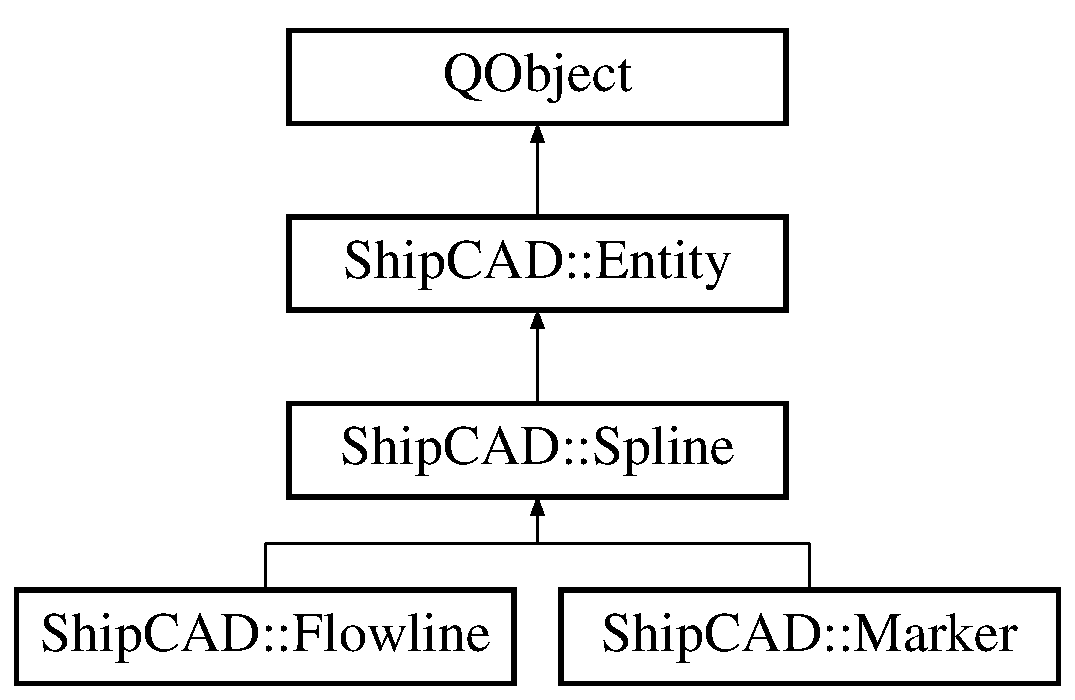
\includegraphics[height=4.000000cm]{classShipCAD_1_1Spline}
\end{center}
\end{figure}
\subsection*{Public Member Functions}
\begin{DoxyCompactItemize}
\item 
\hyperlink{classShipCAD_1_1Spline_a7ad84ea604562c7c9cb309b4e78e25c5}{Spline} ()
\begin{DoxyCompactList}\small\item\em constructor \end{DoxyCompactList}\item 
\hyperlink{classShipCAD_1_1Spline_a891b0c893b8124dca341680076854bff}{Spline} (const \hyperlink{classShipCAD_1_1Spline}{Spline} \&copied)
\begin{DoxyCompactList}\small\item\em copy constructor \end{DoxyCompactList}\item 
virtual \hyperlink{classShipCAD_1_1Spline_a20cddb0145346150b4ca30b63ef47c9b}{$\sim$\+Spline} ()
\begin{DoxyCompactList}\small\item\em destructor \end{DoxyCompactList}\item 
void \hyperlink{classShipCAD_1_1Spline_ac3d9f4514573be91b316413bf062791a}{add} (const Q\+Vector3D \&p)
\begin{DoxyCompactList}\small\item\em add a point to the spline \end{DoxyCompactList}\item 
void \hyperlink{classShipCAD_1_1Spline_a120c5530571f138daad61426053220f3}{delete\+\_\+point} (size\+\_\+t index)
\begin{DoxyCompactList}\small\item\em delete a point from the spline \end{DoxyCompactList}\item 
void \hyperlink{classShipCAD_1_1Spline_aa1ea6446e0b59d5cce88580242cd25b6}{insert} (size\+\_\+t index, const Q\+Vector3D \&p)
\begin{DoxyCompactList}\small\item\em insert a point at the index \end{DoxyCompactList}\item 
void \hyperlink{classShipCAD_1_1Spline_aa8e588b92d23c74bb6ec120624b49e54}{insert\+\_\+spline} (size\+\_\+t index, bool invert, bool duplicate\+\_\+point, const \hyperlink{classShipCAD_1_1Spline}{Spline} \&source)
\begin{DoxyCompactList}\small\item\em insert a copy of a spline at the index \end{DoxyCompactList}\item 
void \hyperlink{classShipCAD_1_1Spline_a26293a4ee636c2b968c45731425d5c94}{invert\+\_\+direction} ()
\begin{DoxyCompactList}\small\item\em invert the direction of this spline \end{DoxyCompactList}\item 
bool \hyperlink{classShipCAD_1_1Spline_a043f418b363a0dc7161b9106a72ef8b4}{simplify} (float criterium)
\begin{DoxyCompactList}\small\item\em simplify the spline by removing points \end{DoxyCompactList}\item 
virtual void \hyperlink{classShipCAD_1_1Spline_a02967f3eee8b1755eab0d7da55c3c621}{clear} ()
\item 
virtual void \hyperlink{classShipCAD_1_1Spline_a9b466ad7510032dafb0421f2d834bde6}{rebuild} ()
\item 
void \hyperlink{classShipCAD_1_1Spline_a6e932411f0f4463514f80011c58f5e6a}{set\+Build} (bool val)
\item 
float \hyperlink{classShipCAD_1_1Spline_a33226d5554ed979f264eb4c6d533145f}{coord\+\_\+length} (float t1, float t2) const 
\item 
float \hyperlink{classShipCAD_1_1Spline_a4e03c541b7c1f96c2fe8d5b1fef558c9}{chord\+\_\+length\+\_\+approximation} (float percentage) const 
\item 
float \hyperlink{classShipCAD_1_1Spline_a755e063448eccbb2714d763596630b9d}{curvature} (float parameter, Q\+Vector3D \&normal) const 
\item 
Q\+Vector3D \hyperlink{classShipCAD_1_1Spline_aff2bf1b4b2e7b5f30e5f2ca35ec93d86}{first\+\_\+derive} (float parameter) const 
\item 
Q\+Vector3D \hyperlink{classShipCAD_1_1Spline_a3c560130edff8a38ed93bf95cf759137}{second\+\_\+derive} (float parameter) const 
\item 
bool \hyperlink{classShipCAD_1_1Spline_ada8dd726a502187bf0e35022576395d3}{intersect\+\_\+plane} (const \hyperlink{classShipCAD_1_1Plane}{Plane} \&plane, \hyperlink{classShipCAD_1_1IntersectionData}{Intersection\+Data} \&output) const 
\item 
Q\+Vector3D \hyperlink{classShipCAD_1_1Spline_aa62cf7afa6461bafce7227ec31875219}{value} (float parameter) const 
\item 
void \hyperlink{classShipCAD_1_1Spline_ae90c8807fb8058d6309f47db64e2d40e}{load\+Binary} (\hyperlink{classShipCAD_1_1FileBuffer}{File\+Buffer} \&source)
\item 
void \hyperlink{classShipCAD_1_1Spline_a5abb8df513d25abe8b0ec000a7926a66}{save\+Binary} (\hyperlink{classShipCAD_1_1FileBuffer}{File\+Buffer} \&destination) const 
\item 
void \hyperlink{classShipCAD_1_1Spline_a33a6300e79043b2fee45cb0eca0696bb}{save\+To\+D\+XF} (Q\+String\+List \&strings, Q\+String layername, bool sendmirror) const 
\item 
virtual void \hyperlink{classShipCAD_1_1Spline_a6424ed433d241f566c15891cc25a74dd}{draw} (\hyperlink{classShipCAD_1_1Viewport}{Viewport} \&vp, \hyperlink{classShipCAD_1_1LineShader}{Line\+Shader} $\ast$lineshader)
\item 
virtual void \hyperlink{classShipCAD_1_1Spline_aa1dcf2a9cff6d17afd926219e3791f9f}{draw\+Starboard} (\hyperlink{classShipCAD_1_1Viewport}{Viewport} \&vp, \hyperlink{classShipCAD_1_1LineShader}{Line\+Shader} $\ast$lineshader)
\item 
bool \hyperlink{classShipCAD_1_1Spline_a2b6fa67f7463838ab2ee9d7b8381a9c5}{show\+Curvature} () const 
\item 
void \hyperlink{classShipCAD_1_1Spline_aae0f5ce3bc2aa58759abd32f3462bf16}{set\+Show\+Curvature} (bool val)
\item 
Q\+Color \hyperlink{classShipCAD_1_1Spline_a788c76b36b091f3d5b92c9cde414cb89}{get\+Curvature\+Color} () const 
\item 
void \hyperlink{classShipCAD_1_1Spline_ac40c22712433f98d657ecaed459d03a0}{set\+Curvature\+Color} (const Q\+Color \&val)
\item 
float \hyperlink{classShipCAD_1_1Spline_af82a5bc6171a9252de5e4c74bf1288e5}{get\+Curvature\+Scale} () const 
\item 
void \hyperlink{classShipCAD_1_1Spline_a17ba0378bfd4a39b4d96d914332c26e4}{set\+Curvature\+Scale} (float val)
\item 
float \hyperlink{classShipCAD_1_1Spline_a81c3cc38d6e70f968b53066bc98e1e01}{get\+Parameter} (size\+\_\+t index) const 
\item 
Q\+Vector3D \hyperlink{classShipCAD_1_1Spline_a04a94537b420a8d19dc5f78526e9a825}{get\+Point} (size\+\_\+t index) const 
\item 
Q\+Vector3D \hyperlink{classShipCAD_1_1Spline_aadd67f56435eea8bb6c74c3aa073c21d}{get\+First\+Point} () const 
\item 
Q\+Vector3D \hyperlink{classShipCAD_1_1Spline_a3e3e7413b8ca8383a93f4770931ed6ed}{get\+Last\+Point} () const 
\item 
void \hyperlink{classShipCAD_1_1Spline_ae02af8d5473f952644ac5103d7beebf2}{set\+Point} (size\+\_\+t index, const Q\+Vector3D \&p)
\item 
size\+\_\+t \hyperlink{classShipCAD_1_1Spline_a58f8c0b2fcc07931a886a85515750e59}{get\+Fragments} () const 
\item 
void \hyperlink{classShipCAD_1_1Spline_aaae6e558fad0833cde71f9ed38e4fb96}{set\+Fragments} (size\+\_\+t val)
\item 
bool \hyperlink{classShipCAD_1_1Spline_aa471e8916034ea3e11c1feb9c8bb935b}{is\+Knuckle} (size\+\_\+t index) const 
\item 
void \hyperlink{classShipCAD_1_1Spline_ad4f075e2e8f1d3ac7c2d22b5be75bbad}{set\+Knuckle} (size\+\_\+t index, bool val)
\item 
size\+\_\+t \hyperlink{classShipCAD_1_1Spline_aa15d52dbfa55ec3b1ec272104a45ebd5}{number\+Of\+Points} () const 
\item 
void \hyperlink{classShipCAD_1_1Spline_a156ffe855d149ad445b178078ee4451c}{dump} (std\+::ostream \&os) const 
\end{DoxyCompactItemize}
\subsection*{Additional Inherited Members}


\subsection{Detailed Description}
spline entity used in intersections etc 

Definition at line 53 of file spline.\+h.



\subsection{Constructor \& Destructor Documentation}
\index{Ship\+C\+A\+D\+::\+Spline@{Ship\+C\+A\+D\+::\+Spline}!Spline@{Spline}}
\index{Spline@{Spline}!Ship\+C\+A\+D\+::\+Spline@{Ship\+C\+A\+D\+::\+Spline}}
\subsubsection[{\texorpdfstring{Spline()}{Spline()}}]{\setlength{\rightskip}{0pt plus 5cm}Spline\+::\+Spline (
\begin{DoxyParamCaption}
{}
\end{DoxyParamCaption}
)\hspace{0.3cm}{\ttfamily [explicit]}}\hypertarget{classShipCAD_1_1Spline_a7ad84ea604562c7c9cb309b4e78e25c5}{}\label{classShipCAD_1_1Spline_a7ad84ea604562c7c9cb309b4e78e25c5}


constructor 



Definition at line 47 of file spline.\+cpp.

\index{Ship\+C\+A\+D\+::\+Spline@{Ship\+C\+A\+D\+::\+Spline}!Spline@{Spline}}
\index{Spline@{Spline}!Ship\+C\+A\+D\+::\+Spline@{Ship\+C\+A\+D\+::\+Spline}}
\subsubsection[{\texorpdfstring{Spline(const Spline \&copied)}{Spline(const Spline &copied)}}]{\setlength{\rightskip}{0pt plus 5cm}Spline\+::\+Spline (
\begin{DoxyParamCaption}
\item[{const {\bf Spline} \&}]{copied}
\end{DoxyParamCaption}
)\hspace{0.3cm}{\ttfamily [explicit]}}\hypertarget{classShipCAD_1_1Spline_a891b0c893b8124dca341680076854bff}{}\label{classShipCAD_1_1Spline_a891b0c893b8124dca341680076854bff}


copy constructor 



Definition at line 53 of file spline.\+cpp.

\index{Ship\+C\+A\+D\+::\+Spline@{Ship\+C\+A\+D\+::\+Spline}!````~Spline@{$\sim$\+Spline}}
\index{````~Spline@{$\sim$\+Spline}!Ship\+C\+A\+D\+::\+Spline@{Ship\+C\+A\+D\+::\+Spline}}
\subsubsection[{\texorpdfstring{$\sim$\+Spline()}{~Spline()}}]{\setlength{\rightskip}{0pt plus 5cm}virtual Ship\+C\+A\+D\+::\+Spline\+::$\sim$\+Spline (
\begin{DoxyParamCaption}
{}
\end{DoxyParamCaption}
)\hspace{0.3cm}{\ttfamily [inline]}, {\ttfamily [virtual]}}\hypertarget{classShipCAD_1_1Spline_a20cddb0145346150b4ca30b63ef47c9b}{}\label{classShipCAD_1_1Spline_a20cddb0145346150b4ca30b63ef47c9b}


destructor 



Definition at line 67 of file spline.\+h.



\subsection{Member Function Documentation}
\index{Ship\+C\+A\+D\+::\+Spline@{Ship\+C\+A\+D\+::\+Spline}!add@{add}}
\index{add@{add}!Ship\+C\+A\+D\+::\+Spline@{Ship\+C\+A\+D\+::\+Spline}}
\subsubsection[{\texorpdfstring{add(const Q\+Vector3\+D \&p)}{add(const QVector3D &p)}}]{\setlength{\rightskip}{0pt plus 5cm}void Spline\+::add (
\begin{DoxyParamCaption}
\item[{const Q\+Vector3D \&}]{p}
\end{DoxyParamCaption}
)}\hypertarget{classShipCAD_1_1Spline_ac3d9f4514573be91b316413bf062791a}{}\label{classShipCAD_1_1Spline_ac3d9f4514573be91b316413bf062791a}


add a point to the spline 


\begin{DoxyParams}{Parameters}
{\em p} & coordinates of point to add \\
\hline
\end{DoxyParams}


Definition at line 371 of file spline.\+cpp.

\index{Ship\+C\+A\+D\+::\+Spline@{Ship\+C\+A\+D\+::\+Spline}!chord\+\_\+length\+\_\+approximation@{chord\+\_\+length\+\_\+approximation}}
\index{chord\+\_\+length\+\_\+approximation@{chord\+\_\+length\+\_\+approximation}!Ship\+C\+A\+D\+::\+Spline@{Ship\+C\+A\+D\+::\+Spline}}
\subsubsection[{\texorpdfstring{chord\+\_\+length\+\_\+approximation(float percentage) const }{chord_length_approximation(float percentage) const }}]{\setlength{\rightskip}{0pt plus 5cm}float Spline\+::chord\+\_\+length\+\_\+approximation (
\begin{DoxyParamCaption}
\item[{float}]{percentage}
\end{DoxyParamCaption}
) const}\hypertarget{classShipCAD_1_1Spline_a4e03c541b7c1f96c2fe8d5b1fef558c9}{}\label{classShipCAD_1_1Spline_a4e03c541b7c1f96c2fe8d5b1fef558c9}


Definition at line 399 of file spline.\+cpp.

\index{Ship\+C\+A\+D\+::\+Spline@{Ship\+C\+A\+D\+::\+Spline}!clear@{clear}}
\index{clear@{clear}!Ship\+C\+A\+D\+::\+Spline@{Ship\+C\+A\+D\+::\+Spline}}
\subsubsection[{\texorpdfstring{clear()}{clear()}}]{\setlength{\rightskip}{0pt plus 5cm}void Spline\+::clear (
\begin{DoxyParamCaption}
{}
\end{DoxyParamCaption}
)\hspace{0.3cm}{\ttfamily [virtual]}}\hypertarget{classShipCAD_1_1Spline_a02967f3eee8b1755eab0d7da55c3c621}{}\label{classShipCAD_1_1Spline_a02967f3eee8b1755eab0d7da55c3c621}


Reimplemented from \hyperlink{classShipCAD_1_1Entity_a998d0e5d360371046fd5835ba1e0877a}{Ship\+C\+A\+D\+::\+Entity}.



Reimplemented in \hyperlink{classShipCAD_1_1Flowline_ac3bbbbd3d853214bb9c9feeb7a12314d}{Ship\+C\+A\+D\+::\+Flowline}, and \hyperlink{classShipCAD_1_1Marker_ac7c7eea8648562f3fa00a9e10af6ec97}{Ship\+C\+A\+D\+::\+Marker}.



Definition at line 790 of file spline.\+cpp.

\index{Ship\+C\+A\+D\+::\+Spline@{Ship\+C\+A\+D\+::\+Spline}!coord\+\_\+length@{coord\+\_\+length}}
\index{coord\+\_\+length@{coord\+\_\+length}!Ship\+C\+A\+D\+::\+Spline@{Ship\+C\+A\+D\+::\+Spline}}
\subsubsection[{\texorpdfstring{coord\+\_\+length(float t1, float t2) const }{coord_length(float t1, float t2) const }}]{\setlength{\rightskip}{0pt plus 5cm}float Spline\+::coord\+\_\+length (
\begin{DoxyParamCaption}
\item[{float}]{t1, }
\item[{float}]{t2}
\end{DoxyParamCaption}
) const}\hypertarget{classShipCAD_1_1Spline_a33226d5554ed979f264eb4c6d533145f}{}\label{classShipCAD_1_1Spline_a33226d5554ed979f264eb4c6d533145f}


Definition at line 379 of file spline.\+cpp.

\index{Ship\+C\+A\+D\+::\+Spline@{Ship\+C\+A\+D\+::\+Spline}!curvature@{curvature}}
\index{curvature@{curvature}!Ship\+C\+A\+D\+::\+Spline@{Ship\+C\+A\+D\+::\+Spline}}
\subsubsection[{\texorpdfstring{curvature(float parameter, Q\+Vector3\+D \&normal) const }{curvature(float parameter, QVector3D &normal) const }}]{\setlength{\rightskip}{0pt plus 5cm}float Spline\+::curvature (
\begin{DoxyParamCaption}
\item[{float}]{parameter, }
\item[{Q\+Vector3D \&}]{normal}
\end{DoxyParamCaption}
) const}\hypertarget{classShipCAD_1_1Spline_a755e063448eccbb2714d763596630b9d}{}\label{classShipCAD_1_1Spline_a755e063448eccbb2714d763596630b9d}


Definition at line 447 of file spline.\+cpp.

\index{Ship\+C\+A\+D\+::\+Spline@{Ship\+C\+A\+D\+::\+Spline}!delete\+\_\+point@{delete\+\_\+point}}
\index{delete\+\_\+point@{delete\+\_\+point}!Ship\+C\+A\+D\+::\+Spline@{Ship\+C\+A\+D\+::\+Spline}}
\subsubsection[{\texorpdfstring{delete\+\_\+point(size\+\_\+t index)}{delete_point(size_t index)}}]{\setlength{\rightskip}{0pt plus 5cm}void Spline\+::delete\+\_\+point (
\begin{DoxyParamCaption}
\item[{size\+\_\+t}]{index}
\end{DoxyParamCaption}
)}\hypertarget{classShipCAD_1_1Spline_a120c5530571f138daad61426053220f3}{}\label{classShipCAD_1_1Spline_a120c5530571f138daad61426053220f3}


delete a point from the spline 


\begin{DoxyParams}{Parameters}
{\em index} & delete point at index \\
\hline
\end{DoxyParams}


Definition at line 469 of file spline.\+cpp.

\index{Ship\+C\+A\+D\+::\+Spline@{Ship\+C\+A\+D\+::\+Spline}!draw@{draw}}
\index{draw@{draw}!Ship\+C\+A\+D\+::\+Spline@{Ship\+C\+A\+D\+::\+Spline}}
\subsubsection[{\texorpdfstring{draw(\+Viewport \&vp, Line\+Shader $\ast$lineshader)}{draw(Viewport &vp, LineShader *lineshader)}}]{\setlength{\rightskip}{0pt plus 5cm}void Spline\+::draw (
\begin{DoxyParamCaption}
\item[{{\bf Viewport} \&}]{vp, }
\item[{{\bf Line\+Shader} $\ast$}]{lineshader}
\end{DoxyParamCaption}
)\hspace{0.3cm}{\ttfamily [virtual]}}\hypertarget{classShipCAD_1_1Spline_a6424ed433d241f566c15891cc25a74dd}{}\label{classShipCAD_1_1Spline_a6424ed433d241f566c15891cc25a74dd}


Implements \hyperlink{classShipCAD_1_1Entity_aa62e306d991140dcd564360f8f6e7539}{Ship\+C\+A\+D\+::\+Entity}.



Reimplemented in \hyperlink{classShipCAD_1_1Flowline_a8b43ac96514f62c6fb0db938eccd0d44}{Ship\+C\+A\+D\+::\+Flowline}, and \hyperlink{classShipCAD_1_1Marker_a0cca647d9b32dc69b03903b024dc3091}{Ship\+C\+A\+D\+::\+Marker}.



Definition at line 507 of file spline.\+cpp.

\index{Ship\+C\+A\+D\+::\+Spline@{Ship\+C\+A\+D\+::\+Spline}!draw\+Starboard@{draw\+Starboard}}
\index{draw\+Starboard@{draw\+Starboard}!Ship\+C\+A\+D\+::\+Spline@{Ship\+C\+A\+D\+::\+Spline}}
\subsubsection[{\texorpdfstring{draw\+Starboard(\+Viewport \&vp, Line\+Shader $\ast$lineshader)}{drawStarboard(Viewport &vp, LineShader *lineshader)}}]{\setlength{\rightskip}{0pt plus 5cm}void Spline\+::draw\+Starboard (
\begin{DoxyParamCaption}
\item[{{\bf Viewport} \&}]{vp, }
\item[{{\bf Line\+Shader} $\ast$}]{lineshader}
\end{DoxyParamCaption}
)\hspace{0.3cm}{\ttfamily [virtual]}}\hypertarget{classShipCAD_1_1Spline_aa1dcf2a9cff6d17afd926219e3791f9f}{}\label{classShipCAD_1_1Spline_aa1dcf2a9cff6d17afd926219e3791f9f}


Definition at line 565 of file spline.\+cpp.

\index{Ship\+C\+A\+D\+::\+Spline@{Ship\+C\+A\+D\+::\+Spline}!dump@{dump}}
\index{dump@{dump}!Ship\+C\+A\+D\+::\+Spline@{Ship\+C\+A\+D\+::\+Spline}}
\subsubsection[{\texorpdfstring{dump(std\+::ostream \&os) const }{dump(std::ostream &os) const }}]{\setlength{\rightskip}{0pt plus 5cm}void Spline\+::dump (
\begin{DoxyParamCaption}
\item[{std\+::ostream \&}]{os}
\end{DoxyParamCaption}
) const}\hypertarget{classShipCAD_1_1Spline_a156ffe855d149ad445b178078ee4451c}{}\label{classShipCAD_1_1Spline_a156ffe855d149ad445b178078ee4451c}


Definition at line 849 of file spline.\+cpp.

\index{Ship\+C\+A\+D\+::\+Spline@{Ship\+C\+A\+D\+::\+Spline}!first\+\_\+derive@{first\+\_\+derive}}
\index{first\+\_\+derive@{first\+\_\+derive}!Ship\+C\+A\+D\+::\+Spline@{Ship\+C\+A\+D\+::\+Spline}}
\subsubsection[{\texorpdfstring{first\+\_\+derive(float parameter) const }{first_derive(float parameter) const }}]{\setlength{\rightskip}{0pt plus 5cm}Q\+Vector3D Spline\+::first\+\_\+derive (
\begin{DoxyParamCaption}
\item[{float}]{parameter}
\end{DoxyParamCaption}
) const}\hypertarget{classShipCAD_1_1Spline_aff2bf1b4b2e7b5f30e5f2ca35ec93d86}{}\label{classShipCAD_1_1Spline_aff2bf1b4b2e7b5f30e5f2ca35ec93d86}


Definition at line 479 of file spline.\+cpp.

\index{Ship\+C\+A\+D\+::\+Spline@{Ship\+C\+A\+D\+::\+Spline}!get\+Curvature\+Color@{get\+Curvature\+Color}}
\index{get\+Curvature\+Color@{get\+Curvature\+Color}!Ship\+C\+A\+D\+::\+Spline@{Ship\+C\+A\+D\+::\+Spline}}
\subsubsection[{\texorpdfstring{get\+Curvature\+Color() const }{getCurvatureColor() const }}]{\setlength{\rightskip}{0pt plus 5cm}Q\+Color Ship\+C\+A\+D\+::\+Spline\+::get\+Curvature\+Color (
\begin{DoxyParamCaption}
{}
\end{DoxyParamCaption}
) const\hspace{0.3cm}{\ttfamily [inline]}}\hypertarget{classShipCAD_1_1Spline_a788c76b36b091f3d5b92c9cde414cb89}{}\label{classShipCAD_1_1Spline_a788c76b36b091f3d5b92c9cde414cb89}


Definition at line 135 of file spline.\+h.

\index{Ship\+C\+A\+D\+::\+Spline@{Ship\+C\+A\+D\+::\+Spline}!get\+Curvature\+Scale@{get\+Curvature\+Scale}}
\index{get\+Curvature\+Scale@{get\+Curvature\+Scale}!Ship\+C\+A\+D\+::\+Spline@{Ship\+C\+A\+D\+::\+Spline}}
\subsubsection[{\texorpdfstring{get\+Curvature\+Scale() const }{getCurvatureScale() const }}]{\setlength{\rightskip}{0pt plus 5cm}float Ship\+C\+A\+D\+::\+Spline\+::get\+Curvature\+Scale (
\begin{DoxyParamCaption}
{}
\end{DoxyParamCaption}
) const\hspace{0.3cm}{\ttfamily [inline]}}\hypertarget{classShipCAD_1_1Spline_af82a5bc6171a9252de5e4c74bf1288e5}{}\label{classShipCAD_1_1Spline_af82a5bc6171a9252de5e4c74bf1288e5}


Definition at line 139 of file spline.\+h.

\index{Ship\+C\+A\+D\+::\+Spline@{Ship\+C\+A\+D\+::\+Spline}!get\+First\+Point@{get\+First\+Point}}
\index{get\+First\+Point@{get\+First\+Point}!Ship\+C\+A\+D\+::\+Spline@{Ship\+C\+A\+D\+::\+Spline}}
\subsubsection[{\texorpdfstring{get\+First\+Point() const }{getFirstPoint() const }}]{\setlength{\rightskip}{0pt plus 5cm}Q\+Vector3D Ship\+C\+A\+D\+::\+Spline\+::get\+First\+Point (
\begin{DoxyParamCaption}
{}
\end{DoxyParamCaption}
) const\hspace{0.3cm}{\ttfamily [inline]}}\hypertarget{classShipCAD_1_1Spline_aadd67f56435eea8bb6c74c3aa073c21d}{}\label{classShipCAD_1_1Spline_aadd67f56435eea8bb6c74c3aa073c21d}


Definition at line 146 of file spline.\+h.

\index{Ship\+C\+A\+D\+::\+Spline@{Ship\+C\+A\+D\+::\+Spline}!get\+Fragments@{get\+Fragments}}
\index{get\+Fragments@{get\+Fragments}!Ship\+C\+A\+D\+::\+Spline@{Ship\+C\+A\+D\+::\+Spline}}
\subsubsection[{\texorpdfstring{get\+Fragments() const }{getFragments() const }}]{\setlength{\rightskip}{0pt plus 5cm}size\+\_\+t Ship\+C\+A\+D\+::\+Spline\+::get\+Fragments (
\begin{DoxyParamCaption}
{}
\end{DoxyParamCaption}
) const\hspace{0.3cm}{\ttfamily [inline]}}\hypertarget{classShipCAD_1_1Spline_a58f8c0b2fcc07931a886a85515750e59}{}\label{classShipCAD_1_1Spline_a58f8c0b2fcc07931a886a85515750e59}


Definition at line 151 of file spline.\+h.

\index{Ship\+C\+A\+D\+::\+Spline@{Ship\+C\+A\+D\+::\+Spline}!get\+Last\+Point@{get\+Last\+Point}}
\index{get\+Last\+Point@{get\+Last\+Point}!Ship\+C\+A\+D\+::\+Spline@{Ship\+C\+A\+D\+::\+Spline}}
\subsubsection[{\texorpdfstring{get\+Last\+Point() const }{getLastPoint() const }}]{\setlength{\rightskip}{0pt plus 5cm}Q\+Vector3D Ship\+C\+A\+D\+::\+Spline\+::get\+Last\+Point (
\begin{DoxyParamCaption}
{}
\end{DoxyParamCaption}
) const\hspace{0.3cm}{\ttfamily [inline]}}\hypertarget{classShipCAD_1_1Spline_a3e3e7413b8ca8383a93f4770931ed6ed}{}\label{classShipCAD_1_1Spline_a3e3e7413b8ca8383a93f4770931ed6ed}


Definition at line 148 of file spline.\+h.

\index{Ship\+C\+A\+D\+::\+Spline@{Ship\+C\+A\+D\+::\+Spline}!get\+Parameter@{get\+Parameter}}
\index{get\+Parameter@{get\+Parameter}!Ship\+C\+A\+D\+::\+Spline@{Ship\+C\+A\+D\+::\+Spline}}
\subsubsection[{\texorpdfstring{get\+Parameter(size\+\_\+t index) const }{getParameter(size_t index) const }}]{\setlength{\rightskip}{0pt plus 5cm}float Spline\+::get\+Parameter (
\begin{DoxyParamCaption}
\item[{size\+\_\+t}]{index}
\end{DoxyParamCaption}
) const}\hypertarget{classShipCAD_1_1Spline_a81c3cc38d6e70f968b53066bc98e1e01}{}\label{classShipCAD_1_1Spline_a81c3cc38d6e70f968b53066bc98e1e01}


Definition at line 77 of file spline.\+cpp.

\index{Ship\+C\+A\+D\+::\+Spline@{Ship\+C\+A\+D\+::\+Spline}!get\+Point@{get\+Point}}
\index{get\+Point@{get\+Point}!Ship\+C\+A\+D\+::\+Spline@{Ship\+C\+A\+D\+::\+Spline}}
\subsubsection[{\texorpdfstring{get\+Point(size\+\_\+t index) const }{getPoint(size_t index) const }}]{\setlength{\rightskip}{0pt plus 5cm}Q\+Vector3D Ship\+C\+A\+D\+::\+Spline\+::get\+Point (
\begin{DoxyParamCaption}
\item[{size\+\_\+t}]{index}
\end{DoxyParamCaption}
) const\hspace{0.3cm}{\ttfamily [inline]}}\hypertarget{classShipCAD_1_1Spline_a04a94537b420a8d19dc5f78526e9a825}{}\label{classShipCAD_1_1Spline_a04a94537b420a8d19dc5f78526e9a825}


Definition at line 144 of file spline.\+h.

\index{Ship\+C\+A\+D\+::\+Spline@{Ship\+C\+A\+D\+::\+Spline}!insert@{insert}}
\index{insert@{insert}!Ship\+C\+A\+D\+::\+Spline@{Ship\+C\+A\+D\+::\+Spline}}
\subsubsection[{\texorpdfstring{insert(size\+\_\+t index, const Q\+Vector3\+D \&p)}{insert(size_t index, const QVector3D &p)}}]{\setlength{\rightskip}{0pt plus 5cm}void Spline\+::insert (
\begin{DoxyParamCaption}
\item[{size\+\_\+t}]{index, }
\item[{const Q\+Vector3D \&}]{p}
\end{DoxyParamCaption}
)}\hypertarget{classShipCAD_1_1Spline_aa1ea6446e0b59d5cce88580242cd25b6}{}\label{classShipCAD_1_1Spline_aa1ea6446e0b59d5cce88580242cd25b6}


insert a point at the index 


\begin{DoxyParams}{Parameters}
{\em index} & where to add the new point \\
\hline
{\em p} & coordinates of new point \\
\hline
\end{DoxyParams}


Definition at line 495 of file spline.\+cpp.

\index{Ship\+C\+A\+D\+::\+Spline@{Ship\+C\+A\+D\+::\+Spline}!insert\+\_\+spline@{insert\+\_\+spline}}
\index{insert\+\_\+spline@{insert\+\_\+spline}!Ship\+C\+A\+D\+::\+Spline@{Ship\+C\+A\+D\+::\+Spline}}
\subsubsection[{\texorpdfstring{insert\+\_\+spline(size\+\_\+t index, bool invert, bool duplicate\+\_\+point, const Spline \&source)}{insert_spline(size_t index, bool invert, bool duplicate_point, const Spline &source)}}]{\setlength{\rightskip}{0pt plus 5cm}void Spline\+::insert\+\_\+spline (
\begin{DoxyParamCaption}
\item[{size\+\_\+t}]{index, }
\item[{bool}]{invert, }
\item[{bool}]{duplicate\+\_\+point, }
\item[{const {\bf Spline} \&}]{source}
\end{DoxyParamCaption}
)}\hypertarget{classShipCAD_1_1Spline_aa8e588b92d23c74bb6ec120624b49e54}{}\label{classShipCAD_1_1Spline_aa8e588b92d23c74bb6ec120624b49e54}


insert a copy of a spline at the index 


\begin{DoxyParams}{Parameters}
{\em index} & where to insert a copy of the spline \\
\hline
{\em invert} & if true, invert the direction of the copied spline \\
\hline
{\em duplicate\+\_\+point} & if true, then the last point of the copied spline is not inserted into this spline \\
\hline
{\em source} & the spline to copy into this spline at the index \\
\hline
\end{DoxyParams}


Definition at line 627 of file spline.\+cpp.

\index{Ship\+C\+A\+D\+::\+Spline@{Ship\+C\+A\+D\+::\+Spline}!intersect\+\_\+plane@{intersect\+\_\+plane}}
\index{intersect\+\_\+plane@{intersect\+\_\+plane}!Ship\+C\+A\+D\+::\+Spline@{Ship\+C\+A\+D\+::\+Spline}}
\subsubsection[{\texorpdfstring{intersect\+\_\+plane(const Plane \&plane, Intersection\+Data \&output) const }{intersect_plane(const Plane &plane, IntersectionData &output) const }}]{\setlength{\rightskip}{0pt plus 5cm}bool Spline\+::intersect\+\_\+plane (
\begin{DoxyParamCaption}
\item[{const {\bf Plane} \&}]{plane, }
\item[{{\bf Intersection\+Data} \&}]{output}
\end{DoxyParamCaption}
) const}\hypertarget{classShipCAD_1_1Spline_ada8dd726a502187bf0e35022576395d3}{}\label{classShipCAD_1_1Spline_ada8dd726a502187bf0e35022576395d3}


Definition at line 666 of file spline.\+cpp.

\index{Ship\+C\+A\+D\+::\+Spline@{Ship\+C\+A\+D\+::\+Spline}!invert\+\_\+direction@{invert\+\_\+direction}}
\index{invert\+\_\+direction@{invert\+\_\+direction}!Ship\+C\+A\+D\+::\+Spline@{Ship\+C\+A\+D\+::\+Spline}}
\subsubsection[{\texorpdfstring{invert\+\_\+direction()}{invert_direction()}}]{\setlength{\rightskip}{0pt plus 5cm}void Spline\+::invert\+\_\+direction (
\begin{DoxyParamCaption}
{}
\end{DoxyParamCaption}
)}\hypertarget{classShipCAD_1_1Spline_a26293a4ee636c2b968c45731425d5c94}{}\label{classShipCAD_1_1Spline_a26293a4ee636c2b968c45731425d5c94}


invert the direction of this spline 



Definition at line 698 of file spline.\+cpp.

\index{Ship\+C\+A\+D\+::\+Spline@{Ship\+C\+A\+D\+::\+Spline}!is\+Knuckle@{is\+Knuckle}}
\index{is\+Knuckle@{is\+Knuckle}!Ship\+C\+A\+D\+::\+Spline@{Ship\+C\+A\+D\+::\+Spline}}
\subsubsection[{\texorpdfstring{is\+Knuckle(size\+\_\+t index) const }{isKnuckle(size_t index) const }}]{\setlength{\rightskip}{0pt plus 5cm}bool Ship\+C\+A\+D\+::\+Spline\+::is\+Knuckle (
\begin{DoxyParamCaption}
\item[{size\+\_\+t}]{index}
\end{DoxyParamCaption}
) const\hspace{0.3cm}{\ttfamily [inline]}}\hypertarget{classShipCAD_1_1Spline_aa471e8916034ea3e11c1feb9c8bb935b}{}\label{classShipCAD_1_1Spline_aa471e8916034ea3e11c1feb9c8bb935b}


Definition at line 154 of file spline.\+h.

\index{Ship\+C\+A\+D\+::\+Spline@{Ship\+C\+A\+D\+::\+Spline}!load\+Binary@{load\+Binary}}
\index{load\+Binary@{load\+Binary}!Ship\+C\+A\+D\+::\+Spline@{Ship\+C\+A\+D\+::\+Spline}}
\subsubsection[{\texorpdfstring{load\+Binary(\+File\+Buffer \&source)}{loadBinary(FileBuffer &source)}}]{\setlength{\rightskip}{0pt plus 5cm}void Spline\+::load\+Binary (
\begin{DoxyParamCaption}
\item[{{\bf File\+Buffer} \&}]{source}
\end{DoxyParamCaption}
)}\hypertarget{classShipCAD_1_1Spline_ae90c8807fb8058d6309f47db64e2d40e}{}\label{classShipCAD_1_1Spline_ae90c8807fb8058d6309f47db64e2d40e}


Definition at line 709 of file spline.\+cpp.

\index{Ship\+C\+A\+D\+::\+Spline@{Ship\+C\+A\+D\+::\+Spline}!number\+Of\+Points@{number\+Of\+Points}}
\index{number\+Of\+Points@{number\+Of\+Points}!Ship\+C\+A\+D\+::\+Spline@{Ship\+C\+A\+D\+::\+Spline}}
\subsubsection[{\texorpdfstring{number\+Of\+Points() const }{numberOfPoints() const }}]{\setlength{\rightskip}{0pt plus 5cm}size\+\_\+t Ship\+C\+A\+D\+::\+Spline\+::number\+Of\+Points (
\begin{DoxyParamCaption}
{}
\end{DoxyParamCaption}
) const\hspace{0.3cm}{\ttfamily [inline]}}\hypertarget{classShipCAD_1_1Spline_aa15d52dbfa55ec3b1ec272104a45ebd5}{}\label{classShipCAD_1_1Spline_aa15d52dbfa55ec3b1ec272104a45ebd5}


Definition at line 157 of file spline.\+h.

\index{Ship\+C\+A\+D\+::\+Spline@{Ship\+C\+A\+D\+::\+Spline}!rebuild@{rebuild}}
\index{rebuild@{rebuild}!Ship\+C\+A\+D\+::\+Spline@{Ship\+C\+A\+D\+::\+Spline}}
\subsubsection[{\texorpdfstring{rebuild()}{rebuild()}}]{\setlength{\rightskip}{0pt plus 5cm}void Spline\+::rebuild (
\begin{DoxyParamCaption}
{}
\end{DoxyParamCaption}
)\hspace{0.3cm}{\ttfamily [virtual]}}\hypertarget{classShipCAD_1_1Spline_a9b466ad7510032dafb0421f2d834bde6}{}\label{classShipCAD_1_1Spline_a9b466ad7510032dafb0421f2d834bde6}


Implements \hyperlink{classShipCAD_1_1Entity_a2571654319df6ad6841a437be7a75395}{Ship\+C\+A\+D\+::\+Entity}.



Reimplemented in \hyperlink{classShipCAD_1_1Flowline_a28e5d73316c6d2c8005428669a9e9b97}{Ship\+C\+A\+D\+::\+Flowline}.



Definition at line 114 of file spline.\+cpp.

\index{Ship\+C\+A\+D\+::\+Spline@{Ship\+C\+A\+D\+::\+Spline}!save\+Binary@{save\+Binary}}
\index{save\+Binary@{save\+Binary}!Ship\+C\+A\+D\+::\+Spline@{Ship\+C\+A\+D\+::\+Spline}}
\subsubsection[{\texorpdfstring{save\+Binary(\+File\+Buffer \&destination) const }{saveBinary(FileBuffer &destination) const }}]{\setlength{\rightskip}{0pt plus 5cm}void Spline\+::save\+Binary (
\begin{DoxyParamCaption}
\item[{{\bf File\+Buffer} \&}]{destination}
\end{DoxyParamCaption}
) const}\hypertarget{classShipCAD_1_1Spline_a5abb8df513d25abe8b0ec000a7926a66}{}\label{classShipCAD_1_1Spline_a5abb8df513d25abe8b0ec000a7926a66}


Definition at line 729 of file spline.\+cpp.

\index{Ship\+C\+A\+D\+::\+Spline@{Ship\+C\+A\+D\+::\+Spline}!save\+To\+D\+XF@{save\+To\+D\+XF}}
\index{save\+To\+D\+XF@{save\+To\+D\+XF}!Ship\+C\+A\+D\+::\+Spline@{Ship\+C\+A\+D\+::\+Spline}}
\subsubsection[{\texorpdfstring{save\+To\+D\+X\+F(\+Q\+String\+List \&strings, Q\+String layername, bool sendmirror) const }{saveToDXF(QStringList &strings, QString layername, bool sendmirror) const }}]{\setlength{\rightskip}{0pt plus 5cm}void Spline\+::save\+To\+D\+XF (
\begin{DoxyParamCaption}
\item[{Q\+String\+List \&}]{strings, }
\item[{Q\+String}]{layername, }
\item[{bool}]{sendmirror}
\end{DoxyParamCaption}
) const}\hypertarget{classShipCAD_1_1Spline_a33a6300e79043b2fee45cb0eca0696bb}{}\label{classShipCAD_1_1Spline_a33a6300e79043b2fee45cb0eca0696bb}


Definition at line 740 of file spline.\+cpp.

\index{Ship\+C\+A\+D\+::\+Spline@{Ship\+C\+A\+D\+::\+Spline}!second\+\_\+derive@{second\+\_\+derive}}
\index{second\+\_\+derive@{second\+\_\+derive}!Ship\+C\+A\+D\+::\+Spline@{Ship\+C\+A\+D\+::\+Spline}}
\subsubsection[{\texorpdfstring{second\+\_\+derive(float parameter) const }{second_derive(float parameter) const }}]{\setlength{\rightskip}{0pt plus 5cm}Q\+Vector3D Spline\+::second\+\_\+derive (
\begin{DoxyParamCaption}
\item[{float}]{parameter}
\end{DoxyParamCaption}
) const}\hypertarget{classShipCAD_1_1Spline_a3c560130edff8a38ed93bf95cf759137}{}\label{classShipCAD_1_1Spline_a3c560130edff8a38ed93bf95cf759137}


Definition at line 230 of file spline.\+cpp.

\index{Ship\+C\+A\+D\+::\+Spline@{Ship\+C\+A\+D\+::\+Spline}!set\+Build@{set\+Build}}
\index{set\+Build@{set\+Build}!Ship\+C\+A\+D\+::\+Spline@{Ship\+C\+A\+D\+::\+Spline}}
\subsubsection[{\texorpdfstring{set\+Build(bool val)}{setBuild(bool val)}}]{\setlength{\rightskip}{0pt plus 5cm}void Spline\+::set\+Build (
\begin{DoxyParamCaption}
\item[{bool}]{val}
\end{DoxyParamCaption}
)\hspace{0.3cm}{\ttfamily [virtual]}}\hypertarget{classShipCAD_1_1Spline_a6e932411f0f4463514f80011c58f5e6a}{}\label{classShipCAD_1_1Spline_a6e932411f0f4463514f80011c58f5e6a}


Reimplemented from \hyperlink{classShipCAD_1_1Entity_a1889198398f42bb7f77a2334031c3f33}{Ship\+C\+A\+D\+::\+Entity}.



Definition at line 65 of file spline.\+cpp.

\index{Ship\+C\+A\+D\+::\+Spline@{Ship\+C\+A\+D\+::\+Spline}!set\+Curvature\+Color@{set\+Curvature\+Color}}
\index{set\+Curvature\+Color@{set\+Curvature\+Color}!Ship\+C\+A\+D\+::\+Spline@{Ship\+C\+A\+D\+::\+Spline}}
\subsubsection[{\texorpdfstring{set\+Curvature\+Color(const Q\+Color \&val)}{setCurvatureColor(const QColor &val)}}]{\setlength{\rightskip}{0pt plus 5cm}void Ship\+C\+A\+D\+::\+Spline\+::set\+Curvature\+Color (
\begin{DoxyParamCaption}
\item[{const Q\+Color \&}]{val}
\end{DoxyParamCaption}
)\hspace{0.3cm}{\ttfamily [inline]}}\hypertarget{classShipCAD_1_1Spline_ac40c22712433f98d657ecaed459d03a0}{}\label{classShipCAD_1_1Spline_ac40c22712433f98d657ecaed459d03a0}


Definition at line 137 of file spline.\+h.

\index{Ship\+C\+A\+D\+::\+Spline@{Ship\+C\+A\+D\+::\+Spline}!set\+Curvature\+Scale@{set\+Curvature\+Scale}}
\index{set\+Curvature\+Scale@{set\+Curvature\+Scale}!Ship\+C\+A\+D\+::\+Spline@{Ship\+C\+A\+D\+::\+Spline}}
\subsubsection[{\texorpdfstring{set\+Curvature\+Scale(float val)}{setCurvatureScale(float val)}}]{\setlength{\rightskip}{0pt plus 5cm}void Ship\+C\+A\+D\+::\+Spline\+::set\+Curvature\+Scale (
\begin{DoxyParamCaption}
\item[{float}]{val}
\end{DoxyParamCaption}
)\hspace{0.3cm}{\ttfamily [inline]}}\hypertarget{classShipCAD_1_1Spline_a17ba0378bfd4a39b4d96d914332c26e4}{}\label{classShipCAD_1_1Spline_a17ba0378bfd4a39b4d96d914332c26e4}


Definition at line 141 of file spline.\+h.

\index{Ship\+C\+A\+D\+::\+Spline@{Ship\+C\+A\+D\+::\+Spline}!set\+Fragments@{set\+Fragments}}
\index{set\+Fragments@{set\+Fragments}!Ship\+C\+A\+D\+::\+Spline@{Ship\+C\+A\+D\+::\+Spline}}
\subsubsection[{\texorpdfstring{set\+Fragments(size\+\_\+t val)}{setFragments(size_t val)}}]{\setlength{\rightskip}{0pt plus 5cm}void Spline\+::set\+Fragments (
\begin{DoxyParamCaption}
\item[{size\+\_\+t}]{val}
\end{DoxyParamCaption}
)}\hypertarget{classShipCAD_1_1Spline_aaae6e558fad0833cde71f9ed38e4fb96}{}\label{classShipCAD_1_1Spline_aaae6e558fad0833cde71f9ed38e4fb96}


Definition at line 84 of file spline.\+cpp.

\index{Ship\+C\+A\+D\+::\+Spline@{Ship\+C\+A\+D\+::\+Spline}!set\+Knuckle@{set\+Knuckle}}
\index{set\+Knuckle@{set\+Knuckle}!Ship\+C\+A\+D\+::\+Spline@{Ship\+C\+A\+D\+::\+Spline}}
\subsubsection[{\texorpdfstring{set\+Knuckle(size\+\_\+t index, bool val)}{setKnuckle(size_t index, bool val)}}]{\setlength{\rightskip}{0pt plus 5cm}void Spline\+::set\+Knuckle (
\begin{DoxyParamCaption}
\item[{size\+\_\+t}]{index, }
\item[{bool}]{val}
\end{DoxyParamCaption}
)}\hypertarget{classShipCAD_1_1Spline_ad4f075e2e8f1d3ac7c2d22b5be75bbad}{}\label{classShipCAD_1_1Spline_ad4f075e2e8f1d3ac7c2d22b5be75bbad}


Definition at line 92 of file spline.\+cpp.

\index{Ship\+C\+A\+D\+::\+Spline@{Ship\+C\+A\+D\+::\+Spline}!set\+Point@{set\+Point}}
\index{set\+Point@{set\+Point}!Ship\+C\+A\+D\+::\+Spline@{Ship\+C\+A\+D\+::\+Spline}}
\subsubsection[{\texorpdfstring{set\+Point(size\+\_\+t index, const Q\+Vector3\+D \&p)}{setPoint(size_t index, const QVector3D &p)}}]{\setlength{\rightskip}{0pt plus 5cm}void Spline\+::set\+Point (
\begin{DoxyParamCaption}
\item[{size\+\_\+t}]{index, }
\item[{const Q\+Vector3D \&}]{p}
\end{DoxyParamCaption}
)}\hypertarget{classShipCAD_1_1Spline_ae02af8d5473f952644ac5103d7beebf2}{}\label{classShipCAD_1_1Spline_ae02af8d5473f952644ac5103d7beebf2}


Definition at line 103 of file spline.\+cpp.

\index{Ship\+C\+A\+D\+::\+Spline@{Ship\+C\+A\+D\+::\+Spline}!set\+Show\+Curvature@{set\+Show\+Curvature}}
\index{set\+Show\+Curvature@{set\+Show\+Curvature}!Ship\+C\+A\+D\+::\+Spline@{Ship\+C\+A\+D\+::\+Spline}}
\subsubsection[{\texorpdfstring{set\+Show\+Curvature(bool val)}{setShowCurvature(bool val)}}]{\setlength{\rightskip}{0pt plus 5cm}void Ship\+C\+A\+D\+::\+Spline\+::set\+Show\+Curvature (
\begin{DoxyParamCaption}
\item[{bool}]{val}
\end{DoxyParamCaption}
)\hspace{0.3cm}{\ttfamily [inline]}}\hypertarget{classShipCAD_1_1Spline_aae0f5ce3bc2aa58759abd32f3462bf16}{}\label{classShipCAD_1_1Spline_aae0f5ce3bc2aa58759abd32f3462bf16}


Definition at line 133 of file spline.\+h.

\index{Ship\+C\+A\+D\+::\+Spline@{Ship\+C\+A\+D\+::\+Spline}!show\+Curvature@{show\+Curvature}}
\index{show\+Curvature@{show\+Curvature}!Ship\+C\+A\+D\+::\+Spline@{Ship\+C\+A\+D\+::\+Spline}}
\subsubsection[{\texorpdfstring{show\+Curvature() const }{showCurvature() const }}]{\setlength{\rightskip}{0pt plus 5cm}bool Ship\+C\+A\+D\+::\+Spline\+::show\+Curvature (
\begin{DoxyParamCaption}
{}
\end{DoxyParamCaption}
) const\hspace{0.3cm}{\ttfamily [inline]}}\hypertarget{classShipCAD_1_1Spline_a2b6fa67f7463838ab2ee9d7b8381a9c5}{}\label{classShipCAD_1_1Spline_a2b6fa67f7463838ab2ee9d7b8381a9c5}


Definition at line 131 of file spline.\+h.

\index{Ship\+C\+A\+D\+::\+Spline@{Ship\+C\+A\+D\+::\+Spline}!simplify@{simplify}}
\index{simplify@{simplify}!Ship\+C\+A\+D\+::\+Spline@{Ship\+C\+A\+D\+::\+Spline}}
\subsubsection[{\texorpdfstring{simplify(float criterium)}{simplify(float criterium)}}]{\setlength{\rightskip}{0pt plus 5cm}bool Spline\+::simplify (
\begin{DoxyParamCaption}
\item[{float}]{criterium}
\end{DoxyParamCaption}
)}\hypertarget{classShipCAD_1_1Spline_a043f418b363a0dc7161b9106a72ef8b4}{}\label{classShipCAD_1_1Spline_a043f418b363a0dc7161b9106a72ef8b4}


simplify the spline by removing points 


\begin{DoxyParams}{Parameters}
{\em criterium} & remove each point that is weighted less than this \\
\hline
\end{DoxyParams}
\begin{DoxyReturn}{Returns}
true if spline is simplified or already simplified 
\end{DoxyReturn}


Definition at line 319 of file spline.\+cpp.

\index{Ship\+C\+A\+D\+::\+Spline@{Ship\+C\+A\+D\+::\+Spline}!value@{value}}
\index{value@{value}!Ship\+C\+A\+D\+::\+Spline@{Ship\+C\+A\+D\+::\+Spline}}
\subsubsection[{\texorpdfstring{value(float parameter) const }{value(float parameter) const }}]{\setlength{\rightskip}{0pt plus 5cm}Q\+Vector3D Spline\+::value (
\begin{DoxyParamCaption}
\item[{float}]{parameter}
\end{DoxyParamCaption}
) const}\hypertarget{classShipCAD_1_1Spline_aa62cf7afa6461bafce7227ec31875219}{}\label{classShipCAD_1_1Spline_aa62cf7afa6461bafce7227ec31875219}


Definition at line 806 of file spline.\+cpp.



The documentation for this class was generated from the following files\+:\begin{DoxyCompactItemize}
\item 
Ship\+C\+A\+Dlib/\hyperlink{spline_8h}{spline.\+h}\item 
Ship\+C\+A\+Dlib/\hyperlink{spline_8cpp}{spline.\+cpp}\end{DoxyCompactItemize}

\hypertarget{structSplineExtents}{}\section{Spline\+Extents Struct Reference}
\label{structSplineExtents}\index{Spline\+Extents@{Spline\+Extents}}
\subsection*{Public Member Functions}
\begin{DoxyCompactItemize}
\item 
\hyperlink{structSplineExtents_ade9a787a7d276d68eef2450f93c932eb}{Spline\+Extents} (Q\+Vector3D \&min, Q\+Vector3D \&max)
\item 
void \hyperlink{structSplineExtents_a8860a15f99d83fd94c3b8068789aa32e}{operator()} (\hyperlink{classShipCAD_1_1Spline}{Spline} $\ast$s)
\end{DoxyCompactItemize}
\subsection*{Public Attributes}
\begin{DoxyCompactItemize}
\item 
Q\+Vector3D \& \hyperlink{structSplineExtents_a6df01932c5ea88c084bf90c67b85afd3}{\+\_\+min}
\item 
Q\+Vector3D \& \hyperlink{structSplineExtents_a22c4af4be35b5646cd88d35b366761d1}{\+\_\+max}
\end{DoxyCompactItemize}


\subsection{Detailed Description}


Definition at line 126 of file intersection.\+cpp.



\subsection{Constructor \& Destructor Documentation}
\index{Spline\+Extents@{Spline\+Extents}!Spline\+Extents@{Spline\+Extents}}
\index{Spline\+Extents@{Spline\+Extents}!Spline\+Extents@{Spline\+Extents}}
\subsubsection[{\texorpdfstring{Spline\+Extents(\+Q\+Vector3\+D \&min, Q\+Vector3\+D \&max)}{SplineExtents(QVector3D &min, QVector3D &max)}}]{\setlength{\rightskip}{0pt plus 5cm}Spline\+Extents\+::\+Spline\+Extents (
\begin{DoxyParamCaption}
\item[{Q\+Vector3D \&}]{min, }
\item[{Q\+Vector3D \&}]{max}
\end{DoxyParamCaption}
)\hspace{0.3cm}{\ttfamily [inline]}}\hypertarget{structSplineExtents_ade9a787a7d276d68eef2450f93c932eb}{}\label{structSplineExtents_ade9a787a7d276d68eef2450f93c932eb}


Definition at line 130 of file intersection.\+cpp.



\subsection{Member Function Documentation}
\index{Spline\+Extents@{Spline\+Extents}!operator()@{operator()}}
\index{operator()@{operator()}!Spline\+Extents@{Spline\+Extents}}
\subsubsection[{\texorpdfstring{operator()(\+Spline $\ast$s)}{operator()(Spline *s)}}]{\setlength{\rightskip}{0pt plus 5cm}void Spline\+Extents\+::operator() (
\begin{DoxyParamCaption}
\item[{{\bf Spline} $\ast$}]{s}
\end{DoxyParamCaption}
)\hspace{0.3cm}{\ttfamily [inline]}}\hypertarget{structSplineExtents_a8860a15f99d83fd94c3b8068789aa32e}{}\label{structSplineExtents_a8860a15f99d83fd94c3b8068789aa32e}


Definition at line 132 of file intersection.\+cpp.



\subsection{Member Data Documentation}
\index{Spline\+Extents@{Spline\+Extents}!\+\_\+max@{\+\_\+max}}
\index{\+\_\+max@{\+\_\+max}!Spline\+Extents@{Spline\+Extents}}
\subsubsection[{\texorpdfstring{\+\_\+max}{_max}}]{\setlength{\rightskip}{0pt plus 5cm}Q\+Vector3D\& Spline\+Extents\+::\+\_\+max}\hypertarget{structSplineExtents_a22c4af4be35b5646cd88d35b366761d1}{}\label{structSplineExtents_a22c4af4be35b5646cd88d35b366761d1}


Definition at line 129 of file intersection.\+cpp.

\index{Spline\+Extents@{Spline\+Extents}!\+\_\+min@{\+\_\+min}}
\index{\+\_\+min@{\+\_\+min}!Spline\+Extents@{Spline\+Extents}}
\subsubsection[{\texorpdfstring{\+\_\+min}{_min}}]{\setlength{\rightskip}{0pt plus 5cm}Q\+Vector3D\& Spline\+Extents\+::\+\_\+min}\hypertarget{structSplineExtents_a6df01932c5ea88c084bf90c67b85afd3}{}\label{structSplineExtents_a6df01932c5ea88c084bf90c67b85afd3}


Definition at line 128 of file intersection.\+cpp.



The documentation for this struct was generated from the following file\+:\begin{DoxyCompactItemize}
\item 
Ship\+C\+A\+Dlib/\hyperlink{intersection_8cpp}{intersection.\+cpp}\end{DoxyCompactItemize}

\hypertarget{structStationAreaCalculation}{}\section{Station\+Area\+Calculation Struct Reference}
\label{structStationAreaCalculation}\index{Station\+Area\+Calculation@{Station\+Area\+Calculation}}
\subsection*{Public Member Functions}
\begin{DoxyCompactItemize}
\item 
\hyperlink{structStationAreaCalculation_aeca509dbb47e4d9eca53b5e0c959dd79}{Station\+Area\+Calculation} (\hyperlink{structShipCAD_1_1HydrostaticsData}{Hydrostatics\+Data} \&d, \hyperlink{classShipCAD_1_1ShipCADModel}{Ship\+C\+A\+D\+Model} $\ast$o)
\item 
void \hyperlink{structStationAreaCalculation_a8f6cf7b08869c75ac1c54bff232ce2ed}{operator()} (\hyperlink{classShipCAD_1_1Intersection}{Intersection} $\ast$intersect)
\end{DoxyCompactItemize}
\subsection*{Public Attributes}
\begin{DoxyCompactItemize}
\item 
\hyperlink{structShipCAD_1_1HydrostaticsData}{Hydrostatics\+Data} \& \hyperlink{structStationAreaCalculation_ad1b380c3cc7135b5d659c7efb5a961c2}{data}
\item 
\hyperlink{classShipCAD_1_1ShipCADModel}{Ship\+C\+A\+D\+Model} $\ast$ \hyperlink{structStationAreaCalculation_a84d2ad6a33b1d6e2db182bebf0a5d7af}{owner}
\end{DoxyCompactItemize}


\subsection{Detailed Description}


Definition at line 902 of file hydrostaticcalc.\+cpp.



\subsection{Constructor \& Destructor Documentation}
\index{Station\+Area\+Calculation@{Station\+Area\+Calculation}!Station\+Area\+Calculation@{Station\+Area\+Calculation}}
\index{Station\+Area\+Calculation@{Station\+Area\+Calculation}!Station\+Area\+Calculation@{Station\+Area\+Calculation}}
\subsubsection[{\texorpdfstring{Station\+Area\+Calculation(\+Hydrostatics\+Data \&d, Ship\+C\+A\+D\+Model $\ast$o)}{StationAreaCalculation(HydrostaticsData &d, ShipCADModel *o)}}]{\setlength{\rightskip}{0pt plus 5cm}Station\+Area\+Calculation\+::\+Station\+Area\+Calculation (
\begin{DoxyParamCaption}
\item[{{\bf Hydrostatics\+Data} \&}]{d, }
\item[{{\bf Ship\+C\+A\+D\+Model} $\ast$}]{o}
\end{DoxyParamCaption}
)\hspace{0.3cm}{\ttfamily [inline]}}\hypertarget{structStationAreaCalculation_aeca509dbb47e4d9eca53b5e0c959dd79}{}\label{structStationAreaCalculation_aeca509dbb47e4d9eca53b5e0c959dd79}


Definition at line 906 of file hydrostaticcalc.\+cpp.



\subsection{Member Function Documentation}
\index{Station\+Area\+Calculation@{Station\+Area\+Calculation}!operator()@{operator()}}
\index{operator()@{operator()}!Station\+Area\+Calculation@{Station\+Area\+Calculation}}
\subsubsection[{\texorpdfstring{operator()(\+Intersection $\ast$intersect)}{operator()(Intersection *intersect)}}]{\setlength{\rightskip}{0pt plus 5cm}void Station\+Area\+Calculation\+::operator() (
\begin{DoxyParamCaption}
\item[{{\bf Intersection} $\ast$}]{intersect}
\end{DoxyParamCaption}
)\hspace{0.3cm}{\ttfamily [inline]}}\hypertarget{structStationAreaCalculation_a8f6cf7b08869c75ac1c54bff232ce2ed}{}\label{structStationAreaCalculation_a8f6cf7b08869c75ac1c54bff232ce2ed}


Definition at line 908 of file hydrostaticcalc.\+cpp.



\subsection{Member Data Documentation}
\index{Station\+Area\+Calculation@{Station\+Area\+Calculation}!data@{data}}
\index{data@{data}!Station\+Area\+Calculation@{Station\+Area\+Calculation}}
\subsubsection[{\texorpdfstring{data}{data}}]{\setlength{\rightskip}{0pt plus 5cm}{\bf Hydrostatics\+Data}\& Station\+Area\+Calculation\+::data}\hypertarget{structStationAreaCalculation_ad1b380c3cc7135b5d659c7efb5a961c2}{}\label{structStationAreaCalculation_ad1b380c3cc7135b5d659c7efb5a961c2}


Definition at line 904 of file hydrostaticcalc.\+cpp.

\index{Station\+Area\+Calculation@{Station\+Area\+Calculation}!owner@{owner}}
\index{owner@{owner}!Station\+Area\+Calculation@{Station\+Area\+Calculation}}
\subsubsection[{\texorpdfstring{owner}{owner}}]{\setlength{\rightskip}{0pt plus 5cm}{\bf Ship\+C\+A\+D\+Model}$\ast$ Station\+Area\+Calculation\+::owner}\hypertarget{structStationAreaCalculation_a84d2ad6a33b1d6e2db182bebf0a5d7af}{}\label{structStationAreaCalculation_a84d2ad6a33b1d6e2db182bebf0a5d7af}


Definition at line 905 of file hydrostaticcalc.\+cpp.



The documentation for this struct was generated from the following file\+:\begin{DoxyCompactItemize}
\item 
Ship\+C\+A\+Dlib/\hyperlink{hydrostaticcalc_8cpp}{hydrostaticcalc.\+cpp}\end{DoxyCompactItemize}

\hypertarget{classShipCAD_1_1SubdivisionBase}{}\section{Ship\+C\+AD\+:\+:Subdivision\+Base Class Reference}
\label{classShipCAD_1_1SubdivisionBase}\index{Ship\+C\+A\+D\+::\+Subdivision\+Base@{Ship\+C\+A\+D\+::\+Subdivision\+Base}}


the base class for all subdivision points, edges and faces  




{\ttfamily \#include $<$subdivbase.\+h$>$}

Inheritance diagram for Ship\+C\+AD\+:\+:Subdivision\+Base\+:\begin{figure}[H]
\begin{center}
\leavevmode
\includegraphics[height=1.534247cm]{classShipCAD_1_1SubdivisionBase}
\end{center}
\end{figure}
\subsection*{Public Member Functions}
\begin{DoxyCompactItemize}
\item 
\hyperlink{classShipCAD_1_1SubdivisionBase_ad424b99e73d138f565a152ed0ee648cb}{Subdivision\+Base} (\hyperlink{classShipCAD_1_1SubdivisionSurface}{Subdivision\+Surface} $\ast$owner)
\begin{DoxyCompactList}\small\item\em Constructor. \end{DoxyCompactList}\item 
virtual \hyperlink{classShipCAD_1_1SubdivisionBase_a12b4adebcd9fb52d4d82d9ff469e144d}{$\sim$\+Subdivision\+Base} ()
\item 
\hyperlink{classShipCAD_1_1SubdivisionSurface}{Subdivision\+Surface} $\ast$ \hyperlink{classShipCAD_1_1SubdivisionBase_a0b9a68b5c7e6a20cf52a465f2387ffba}{get\+Owner} ()
\begin{DoxyCompactList}\small\item\em get the owning surface \end{DoxyCompactList}\item 
const \hyperlink{classShipCAD_1_1SubdivisionSurface}{Subdivision\+Surface} $\ast$ \hyperlink{classShipCAD_1_1SubdivisionBase_a8e98f69a132bcc75a0f6515b7a8a80f5}{get\+Owner} () const 
\begin{DoxyCompactList}\small\item\em get the owning surface \end{DoxyCompactList}\item 
virtual void \hyperlink{classShipCAD_1_1SubdivisionBase_a8f64480f79c9260facc2d27cd19a36ed}{set\+Owner} (\hyperlink{classShipCAD_1_1SubdivisionSurface}{Subdivision\+Surface} $\ast$newowner)
\begin{DoxyCompactList}\small\item\em set the owing surface \end{DoxyCompactList}\item 
virtual void \hyperlink{classShipCAD_1_1SubdivisionBase_a851bb7f1931f9dd6e53b6f9df7b5b352}{clear} ()=0
\begin{DoxyCompactList}\small\item\em reset this element to default values \end{DoxyCompactList}\item 
virtual void \hyperlink{classShipCAD_1_1SubdivisionBase_a7807e64ac8d2acc3da572e03cf0523b6}{dump} (std\+::ostream \&os, const char $\ast$prefix=\char`\"{}\char`\"{}) const 
\begin{DoxyCompactList}\small\item\em print out the element to a stream \end{DoxyCompactList}\end{DoxyCompactItemize}
\subsection*{Protected Member Functions}
\begin{DoxyCompactItemize}
\item 
void \hyperlink{classShipCAD_1_1SubdivisionBase_a024aa781bbf2e54b6fb088e33126998e}{priv\+\_\+dump} (std\+::ostream \&os, const char $\ast$prefix) const 
\begin{DoxyCompactList}\small\item\em dump the element to a stream \end{DoxyCompactList}\end{DoxyCompactItemize}
\subsection*{Protected Attributes}
\begin{DoxyCompactItemize}
\item 
\hyperlink{classShipCAD_1_1SubdivisionSurface}{Subdivision\+Surface} $\ast$ \hyperlink{classShipCAD_1_1SubdivisionBase_a164481259436bf18bc22a0626ab66c09}{\+\_\+owner}
\end{DoxyCompactItemize}


\subsection{Detailed Description}
the base class for all subdivision points, edges and faces 



Definition at line 45 of file subdivbase.\+h.



\subsection{Constructor \& Destructor Documentation}
\index{Ship\+C\+A\+D\+::\+Subdivision\+Base@{Ship\+C\+A\+D\+::\+Subdivision\+Base}!Subdivision\+Base@{Subdivision\+Base}}
\index{Subdivision\+Base@{Subdivision\+Base}!Ship\+C\+A\+D\+::\+Subdivision\+Base@{Ship\+C\+A\+D\+::\+Subdivision\+Base}}
\subsubsection[{\texorpdfstring{Subdivision\+Base(\+Subdivision\+Surface $\ast$owner)}{SubdivisionBase(SubdivisionSurface *owner)}}]{\setlength{\rightskip}{0pt plus 5cm}Subdivision\+Base\+::\+Subdivision\+Base (
\begin{DoxyParamCaption}
\item[{{\bf Subdivision\+Surface} $\ast$}]{owner}
\end{DoxyParamCaption}
)\hspace{0.3cm}{\ttfamily [explicit]}}\hypertarget{classShipCAD_1_1SubdivisionBase_ad424b99e73d138f565a152ed0ee648cb}{}\label{classShipCAD_1_1SubdivisionBase_ad424b99e73d138f565a152ed0ee648cb}


Constructor. 


\begin{DoxyParams}{Parameters}
{\em owner} & which surface this element belongs to \\
\hline
\end{DoxyParams}


Definition at line 40 of file subdivbase.\+cpp.

\index{Ship\+C\+A\+D\+::\+Subdivision\+Base@{Ship\+C\+A\+D\+::\+Subdivision\+Base}!````~Subdivision\+Base@{$\sim$\+Subdivision\+Base}}
\index{````~Subdivision\+Base@{$\sim$\+Subdivision\+Base}!Ship\+C\+A\+D\+::\+Subdivision\+Base@{Ship\+C\+A\+D\+::\+Subdivision\+Base}}
\subsubsection[{\texorpdfstring{$\sim$\+Subdivision\+Base()}{~SubdivisionBase()}}]{\setlength{\rightskip}{0pt plus 5cm}Subdivision\+Base\+::$\sim$\+Subdivision\+Base (
\begin{DoxyParamCaption}
{}
\end{DoxyParamCaption}
)\hspace{0.3cm}{\ttfamily [virtual]}}\hypertarget{classShipCAD_1_1SubdivisionBase_a12b4adebcd9fb52d4d82d9ff469e144d}{}\label{classShipCAD_1_1SubdivisionBase_a12b4adebcd9fb52d4d82d9ff469e144d}


Definition at line 46 of file subdivbase.\+cpp.



\subsection{Member Function Documentation}
\index{Ship\+C\+A\+D\+::\+Subdivision\+Base@{Ship\+C\+A\+D\+::\+Subdivision\+Base}!clear@{clear}}
\index{clear@{clear}!Ship\+C\+A\+D\+::\+Subdivision\+Base@{Ship\+C\+A\+D\+::\+Subdivision\+Base}}
\subsubsection[{\texorpdfstring{clear()=0}{clear()=0}}]{\setlength{\rightskip}{0pt plus 5cm}virtual void Ship\+C\+A\+D\+::\+Subdivision\+Base\+::clear (
\begin{DoxyParamCaption}
{}
\end{DoxyParamCaption}
)\hspace{0.3cm}{\ttfamily [pure virtual]}}\hypertarget{classShipCAD_1_1SubdivisionBase_a851bb7f1931f9dd6e53b6f9df7b5b352}{}\label{classShipCAD_1_1SubdivisionBase_a851bb7f1931f9dd6e53b6f9df7b5b352}


reset this element to default values 



Implemented in \hyperlink{classShipCAD_1_1SubdivisionControlFace_ad168e31f0ef2537b3cd0f58b0c1c54e2}{Ship\+C\+A\+D\+::\+Subdivision\+Control\+Face}, \hyperlink{classShipCAD_1_1SubdivisionFace_a413ae7e76f559780c8a69e998974fb75}{Ship\+C\+A\+D\+::\+Subdivision\+Face}, \hyperlink{classShipCAD_1_1SubdivisionLayer_a7046d17ba87dd5ce7399f22ae327fc6e}{Ship\+C\+A\+D\+::\+Subdivision\+Layer}, \hyperlink{classShipCAD_1_1SubdivisionPoint_aef22d2b6cb48e57ce69652eeb7a69711}{Ship\+C\+A\+D\+::\+Subdivision\+Point}, \hyperlink{classShipCAD_1_1SubdivisionControlCurve_aa574f77f4abc5a8eef05e7cef7f8d8a2}{Ship\+C\+A\+D\+::\+Subdivision\+Control\+Curve}, and \hyperlink{classShipCAD_1_1SubdivisionEdge_a08358ac65c2d710855b8b93c64ce9d02}{Ship\+C\+A\+D\+::\+Subdivision\+Edge}.

\index{Ship\+C\+A\+D\+::\+Subdivision\+Base@{Ship\+C\+A\+D\+::\+Subdivision\+Base}!dump@{dump}}
\index{dump@{dump}!Ship\+C\+A\+D\+::\+Subdivision\+Base@{Ship\+C\+A\+D\+::\+Subdivision\+Base}}
\subsubsection[{\texorpdfstring{dump(std\+::ostream \&os, const char $\ast$prefix="""") const }{dump(std::ostream &os, const char *prefix="") const }}]{\setlength{\rightskip}{0pt plus 5cm}void Subdivision\+Base\+::dump (
\begin{DoxyParamCaption}
\item[{std\+::ostream \&}]{os, }
\item[{const char $\ast$}]{prefix = {\ttfamily \char`\"{}\char`\"{}}}
\end{DoxyParamCaption}
) const\hspace{0.3cm}{\ttfamily [virtual]}}\hypertarget{classShipCAD_1_1SubdivisionBase_a7807e64ac8d2acc3da572e03cf0523b6}{}\label{classShipCAD_1_1SubdivisionBase_a7807e64ac8d2acc3da572e03cf0523b6}


print out the element to a stream 


\begin{DoxyParams}{Parameters}
{\em os} & the output stream \\
\hline
{\em prefix} & string to prefix on each line output \\
\hline
\end{DoxyParams}


Reimplemented in \hyperlink{classShipCAD_1_1SubdivisionControlFace_a947868fba3e9bb6c587847fb9245c9ff}{Ship\+C\+A\+D\+::\+Subdivision\+Control\+Face}, \hyperlink{classShipCAD_1_1SubdivisionControlPoint_a4a9d6e45291c27f19f0d76c9b9d19048}{Ship\+C\+A\+D\+::\+Subdivision\+Control\+Point}, \hyperlink{classShipCAD_1_1SubdivisionFace_aa5bd261ae5fc0a1c7fe8cc5328b8477f}{Ship\+C\+A\+D\+::\+Subdivision\+Face}, \hyperlink{classShipCAD_1_1SubdivisionPoint_aed72cf5e8dc67e980010d195f3a376a3}{Ship\+C\+A\+D\+::\+Subdivision\+Point}, \hyperlink{classShipCAD_1_1SubdivisionControlEdge_abdfa96ff05eff404214a92d38d7eb715}{Ship\+C\+A\+D\+::\+Subdivision\+Control\+Edge}, \hyperlink{classShipCAD_1_1SubdivisionLayer_ab41e005f720a2bba4b2efa74bfd5943e}{Ship\+C\+A\+D\+::\+Subdivision\+Layer}, \hyperlink{classShipCAD_1_1SubdivisionControlCurve_a30e8d074583a386be2ab6343cb5f8502}{Ship\+C\+A\+D\+::\+Subdivision\+Control\+Curve}, and \hyperlink{classShipCAD_1_1SubdivisionEdge_a14cc58877644ebd7b7ebffbdf8ef87f7}{Ship\+C\+A\+D\+::\+Subdivision\+Edge}.



Definition at line 51 of file subdivbase.\+cpp.

\index{Ship\+C\+A\+D\+::\+Subdivision\+Base@{Ship\+C\+A\+D\+::\+Subdivision\+Base}!get\+Owner@{get\+Owner}}
\index{get\+Owner@{get\+Owner}!Ship\+C\+A\+D\+::\+Subdivision\+Base@{Ship\+C\+A\+D\+::\+Subdivision\+Base}}
\subsubsection[{\texorpdfstring{get\+Owner()}{getOwner()}}]{\setlength{\rightskip}{0pt plus 5cm}{\bf Subdivision\+Surface}$\ast$ Ship\+C\+A\+D\+::\+Subdivision\+Base\+::get\+Owner (
\begin{DoxyParamCaption}
{}
\end{DoxyParamCaption}
)\hspace{0.3cm}{\ttfamily [inline]}}\hypertarget{classShipCAD_1_1SubdivisionBase_a0b9a68b5c7e6a20cf52a465f2387ffba}{}\label{classShipCAD_1_1SubdivisionBase_a0b9a68b5c7e6a20cf52a465f2387ffba}


get the owning surface 

\begin{DoxyReturn}{Returns}
the owning surface 
\end{DoxyReturn}


Definition at line 60 of file subdivbase.\+h.

\index{Ship\+C\+A\+D\+::\+Subdivision\+Base@{Ship\+C\+A\+D\+::\+Subdivision\+Base}!get\+Owner@{get\+Owner}}
\index{get\+Owner@{get\+Owner}!Ship\+C\+A\+D\+::\+Subdivision\+Base@{Ship\+C\+A\+D\+::\+Subdivision\+Base}}
\subsubsection[{\texorpdfstring{get\+Owner() const }{getOwner() const }}]{\setlength{\rightskip}{0pt plus 5cm}const {\bf Subdivision\+Surface}$\ast$ Ship\+C\+A\+D\+::\+Subdivision\+Base\+::get\+Owner (
\begin{DoxyParamCaption}
{}
\end{DoxyParamCaption}
) const\hspace{0.3cm}{\ttfamily [inline]}}\hypertarget{classShipCAD_1_1SubdivisionBase_a8e98f69a132bcc75a0f6515b7a8a80f5}{}\label{classShipCAD_1_1SubdivisionBase_a8e98f69a132bcc75a0f6515b7a8a80f5}


get the owning surface 

\begin{DoxyReturn}{Returns}
the owning surface 
\end{DoxyReturn}


Definition at line 65 of file subdivbase.\+h.

\index{Ship\+C\+A\+D\+::\+Subdivision\+Base@{Ship\+C\+A\+D\+::\+Subdivision\+Base}!priv\+\_\+dump@{priv\+\_\+dump}}
\index{priv\+\_\+dump@{priv\+\_\+dump}!Ship\+C\+A\+D\+::\+Subdivision\+Base@{Ship\+C\+A\+D\+::\+Subdivision\+Base}}
\subsubsection[{\texorpdfstring{priv\+\_\+dump(std\+::ostream \&os, const char $\ast$prefix) const }{priv_dump(std::ostream &os, const char *prefix) const }}]{\setlength{\rightskip}{0pt plus 5cm}void Subdivision\+Base\+::priv\+\_\+dump (
\begin{DoxyParamCaption}
\item[{std\+::ostream \&}]{os, }
\item[{const char $\ast$}]{prefix}
\end{DoxyParamCaption}
) const\hspace{0.3cm}{\ttfamily [protected]}}\hypertarget{classShipCAD_1_1SubdivisionBase_a024aa781bbf2e54b6fb088e33126998e}{}\label{classShipCAD_1_1SubdivisionBase_a024aa781bbf2e54b6fb088e33126998e}


dump the element to a stream 


\begin{DoxyParams}{Parameters}
{\em os} & the output stream \\
\hline
{\em prefix} & string to prefix on each line output \\
\hline
\end{DoxyParams}


Definition at line 57 of file subdivbase.\+cpp.

\index{Ship\+C\+A\+D\+::\+Subdivision\+Base@{Ship\+C\+A\+D\+::\+Subdivision\+Base}!set\+Owner@{set\+Owner}}
\index{set\+Owner@{set\+Owner}!Ship\+C\+A\+D\+::\+Subdivision\+Base@{Ship\+C\+A\+D\+::\+Subdivision\+Base}}
\subsubsection[{\texorpdfstring{set\+Owner(\+Subdivision\+Surface $\ast$newowner)}{setOwner(SubdivisionSurface *newowner)}}]{\setlength{\rightskip}{0pt plus 5cm}virtual void Ship\+C\+A\+D\+::\+Subdivision\+Base\+::set\+Owner (
\begin{DoxyParamCaption}
\item[{{\bf Subdivision\+Surface} $\ast$}]{newowner}
\end{DoxyParamCaption}
)\hspace{0.3cm}{\ttfamily [inline]}, {\ttfamily [virtual]}}\hypertarget{classShipCAD_1_1SubdivisionBase_a8f64480f79c9260facc2d27cd19a36ed}{}\label{classShipCAD_1_1SubdivisionBase_a8f64480f79c9260facc2d27cd19a36ed}


set the owing surface 


\begin{DoxyParams}{Parameters}
{\em newowner} & the owning surface \\
\hline
\end{DoxyParams}


Definition at line 70 of file subdivbase.\+h.



\subsection{Member Data Documentation}
\index{Ship\+C\+A\+D\+::\+Subdivision\+Base@{Ship\+C\+A\+D\+::\+Subdivision\+Base}!\+\_\+owner@{\+\_\+owner}}
\index{\+\_\+owner@{\+\_\+owner}!Ship\+C\+A\+D\+::\+Subdivision\+Base@{Ship\+C\+A\+D\+::\+Subdivision\+Base}}
\subsubsection[{\texorpdfstring{\+\_\+owner}{_owner}}]{\setlength{\rightskip}{0pt plus 5cm}{\bf Subdivision\+Surface}$\ast$ Ship\+C\+A\+D\+::\+Subdivision\+Base\+::\+\_\+owner\hspace{0.3cm}{\ttfamily [protected]}}\hypertarget{classShipCAD_1_1SubdivisionBase_a164481259436bf18bc22a0626ab66c09}{}\label{classShipCAD_1_1SubdivisionBase_a164481259436bf18bc22a0626ab66c09}
the owning surface 

Definition at line 95 of file subdivbase.\+h.



The documentation for this class was generated from the following files\+:\begin{DoxyCompactItemize}
\item 
Ship\+C\+A\+Dlib/\hyperlink{subdivbase_8h}{subdivbase.\+h}\item 
Ship\+C\+A\+Dlib/\hyperlink{subdivbase_8cpp}{subdivbase.\+cpp}\end{DoxyCompactItemize}

\hypertarget{classShipCAD_1_1SubdivisionControlCurve}{}\section{Ship\+C\+AD\+:\+:Subdivision\+Control\+Curve Class Reference}
\label{classShipCAD_1_1SubdivisionControlCurve}\index{Ship\+C\+A\+D\+::\+Subdivision\+Control\+Curve@{Ship\+C\+A\+D\+::\+Subdivision\+Control\+Curve}}


{\ttfamily \#include $<$subdivcontrolcurve.\+h$>$}

Inheritance diagram for Ship\+C\+AD\+:\+:Subdivision\+Control\+Curve\+:\begin{figure}[H]
\begin{center}
\leavevmode
\includegraphics[height=2.000000cm]{classShipCAD_1_1SubdivisionControlCurve}
\end{center}
\end{figure}
\subsection*{Public Member Functions}
\begin{DoxyCompactItemize}
\item 
\hyperlink{classShipCAD_1_1SubdivisionControlCurve_a6655333ddb8fa6c464dba4f6f7776592}{Subdivision\+Control\+Curve} (\hyperlink{classShipCAD_1_1SubdivisionSurface}{Subdivision\+Surface} $\ast$owner, \hyperlink{classShipCAD_1_1Spline}{Spline} $\ast$spline)
\item 
virtual \hyperlink{classShipCAD_1_1SubdivisionControlCurve_ab8df7be8d521f9b0bc5c7e8fd0156eef}{$\sim$\+Subdivision\+Control\+Curve} ()
\item 
void \hyperlink{classShipCAD_1_1SubdivisionControlCurve_a6e2678c3fa1885e63d11bb692af54af7}{remove\+Curve} ()
\item 
void \hyperlink{classShipCAD_1_1SubdivisionControlCurve_a078fc8820a6c0e37c475eec1897b13dd}{replace\+Vertex\+Point} (\hyperlink{classShipCAD_1_1SubdivisionPoint}{Subdivision\+Point} $\ast$oldpt, \hyperlink{classShipCAD_1_1SubdivisionPoint}{Subdivision\+Point} $\ast$newpt)
\item 
void \hyperlink{classShipCAD_1_1SubdivisionControlCurve_a0764f5d7697b76ac928a121d224733f5}{insert\+Edge\+Point} (\hyperlink{classShipCAD_1_1SubdivisionPoint}{Subdivision\+Point} $\ast$p1, \hyperlink{classShipCAD_1_1SubdivisionPoint}{Subdivision\+Point} $\ast$p2, \hyperlink{classShipCAD_1_1SubdivisionPoint}{Subdivision\+Point} $\ast$newpt)
\item 
void \hyperlink{classShipCAD_1_1SubdivisionControlCurve_abfed48331919c4d2a2bfc6363b28ebb4}{delete\+Edge} (\hyperlink{classShipCAD_1_1SubdivisionControlEdge}{Subdivision\+Control\+Edge} $\ast$edge)
\item 
void \hyperlink{classShipCAD_1_1SubdivisionControlCurve_a9469b178a88269d0f9ee3b17d5f15272}{insert\+Control\+Point} (\hyperlink{classShipCAD_1_1SubdivisionControlPoint}{Subdivision\+Control\+Point} $\ast$p1, \hyperlink{classShipCAD_1_1SubdivisionControlPoint}{Subdivision\+Control\+Point} $\ast$p2, \hyperlink{classShipCAD_1_1SubdivisionControlPoint}{Subdivision\+Control\+Point} $\ast$newpt)
\item 
void \hyperlink{classShipCAD_1_1SubdivisionControlCurve_a1155b0abe401a7128369a589b6e6ac9c}{add\+Point} (\hyperlink{classShipCAD_1_1SubdivisionControlPoint}{Subdivision\+Control\+Point} $\ast$p)
\item 
virtual void \hyperlink{classShipCAD_1_1SubdivisionControlCurve_aa574f77f4abc5a8eef05e7cef7f8d8a2}{clear} ()
\begin{DoxyCompactList}\small\item\em reset this element to default values \end{DoxyCompactList}\item 
void \hyperlink{classShipCAD_1_1SubdivisionControlCurve_a34e280e9ba6e6705577d1afd229e9f20}{reset\+Div\+Points} ()
\item 
bool \hyperlink{classShipCAD_1_1SubdivisionControlCurve_ae4a8eda1eb14cc85f336aa6b2d10753b}{is\+Selected} () const 
\item 
bool \hyperlink{classShipCAD_1_1SubdivisionControlCurve_a5ed850eb8b536f4f534adca1c9a3aca0}{is\+Visible} () const 
\item 
bool \hyperlink{classShipCAD_1_1SubdivisionControlCurve_ab1f7193c8129646d289aebf5d2d58ef7}{is\+Build} () const 
\item 
Q\+Color \hyperlink{classShipCAD_1_1SubdivisionControlCurve_a800e0d38d3cdbdc6a38aa989b5fdb3ff}{get\+Color} () const 
\item 
size\+\_\+t \hyperlink{classShipCAD_1_1SubdivisionControlCurve_ae5fbcecbf686e25e28a6b418719e8ecb}{number\+Of\+Control\+Points} () const 
\item 
size\+\_\+t \hyperlink{classShipCAD_1_1SubdivisionControlCurve_a15005a440eec6919d9fae9ff92cdf566}{number\+Of\+Subdiv\+Points} () const 
\item 
\hyperlink{classShipCAD_1_1SubdivisionControlPoint}{Subdivision\+Control\+Point} $\ast$ \hyperlink{classShipCAD_1_1SubdivisionControlCurve_a40ad888b65a29ca25d39a15f37cb53c0}{get\+Control\+Point} (size\+\_\+t index) const 
\item 
\hyperlink{classShipCAD_1_1SubdivisionPoint}{Subdivision\+Point} $\ast$ \hyperlink{classShipCAD_1_1SubdivisionControlCurve_ad34aef8d1a8bd36a68299d3eca67d056}{get\+Subdiv\+Point} (size\+\_\+t index) const 
\item 
void \hyperlink{classShipCAD_1_1SubdivisionControlCurve_ac536de424624a4ae312029fe643f4b61}{set\+Visible} (bool val)
\item 
void \hyperlink{classShipCAD_1_1SubdivisionControlCurve_afb98b225e0dc255272a69e96c14eedb7}{set\+Build} (bool val)
\item 
void \hyperlink{classShipCAD_1_1SubdivisionControlCurve_abaf7f7cfec21eedacf55b1654f3e7f2f}{set\+Selected} (bool val)
\item 
\hyperlink{classShipCAD_1_1Spline}{Spline} $\ast$ \hyperlink{classShipCAD_1_1SubdivisionControlCurve_af40e4673307d023a6763e0ba64fd47dd}{get\+Spline} () const 
\item 
void \hyperlink{classShipCAD_1_1SubdivisionControlCurve_ad2a7118ea074ce1b7f61586f08039d2a}{load\+Binary} (\hyperlink{classShipCAD_1_1FileBuffer}{File\+Buffer} \&source)
\item 
void \hyperlink{classShipCAD_1_1SubdivisionControlCurve_a6b7ecd29d30f2eb0625094e514f0e542}{save\+Binary} (\hyperlink{classShipCAD_1_1FileBuffer}{File\+Buffer} \&destination) const 
\item 
void \hyperlink{classShipCAD_1_1SubdivisionControlCurve_a9bd87373607e0b916e340f61b5c22750}{save\+To\+D\+XF} (Q\+String\+List \&strings) const 
\item 
virtual void \hyperlink{classShipCAD_1_1SubdivisionControlCurve_a4d7d8e87dc582529e763039ffe593360}{draw} (\hyperlink{classShipCAD_1_1Viewport}{Viewport} \&vp, \hyperlink{classShipCAD_1_1LineShader}{Line\+Shader} $\ast$lineshader)
\item 
virtual void \hyperlink{classShipCAD_1_1SubdivisionControlCurve_a30e8d074583a386be2ab6343cb5f8502}{dump} (std\+::ostream \&os, const char $\ast$prefix=\char`\"{}\char`\"{}) const 
\begin{DoxyCompactList}\small\item\em print out the element to a stream \end{DoxyCompactList}\end{DoxyCompactItemize}
\subsection*{Static Public Member Functions}
\begin{DoxyCompactItemize}
\item 
static \hyperlink{classShipCAD_1_1SubdivisionControlCurve}{Subdivision\+Control\+Curve} $\ast$ \hyperlink{classShipCAD_1_1SubdivisionControlCurve_a21d9226cc2fd7efcaf6f1067912a0b34}{construct} (\hyperlink{classShipCAD_1_1SubdivisionSurface}{Subdivision\+Surface} $\ast$owner)
\end{DoxyCompactItemize}
\subsection*{Protected Member Functions}
\begin{DoxyCompactItemize}
\item 
void \hyperlink{classShipCAD_1_1SubdivisionControlCurve_a48fbb761e8c85120ba7f6876d873e898}{priv\+\_\+dump} (std\+::ostream \&os, const char $\ast$prefix) const 
\end{DoxyCompactItemize}
\subsection*{Protected Attributes}
\begin{DoxyCompactItemize}
\item 
bool \hyperlink{classShipCAD_1_1SubdivisionControlCurve_a1e4dd9968f46becb714e44709d0da418}{\+\_\+build}
\item 
std\+::vector$<$ \hyperlink{classShipCAD_1_1SubdivisionControlPoint}{Subdivision\+Control\+Point} $\ast$ $>$ \hyperlink{classShipCAD_1_1SubdivisionControlCurve_ac54ea0783b3f8f2aa65d49fe489f1b4f}{\+\_\+points}
\item 
std\+::vector$<$ \hyperlink{classShipCAD_1_1SubdivisionPoint}{Subdivision\+Point} $\ast$ $>$ \hyperlink{classShipCAD_1_1SubdivisionControlCurve_af91dbc96b703fe618567326cca21d82c}{\+\_\+div\+\_\+points}
\item 
\hyperlink{classShipCAD_1_1Spline}{Spline} $\ast$ \hyperlink{classShipCAD_1_1SubdivisionControlCurve_a115a5b67ed81a3012ccb02a25b3d2c24}{\+\_\+curve}
\end{DoxyCompactItemize}


\subsection{Detailed Description}


Definition at line 56 of file subdivcontrolcurve.\+h.



\subsection{Constructor \& Destructor Documentation}
\index{Ship\+C\+A\+D\+::\+Subdivision\+Control\+Curve@{Ship\+C\+A\+D\+::\+Subdivision\+Control\+Curve}!Subdivision\+Control\+Curve@{Subdivision\+Control\+Curve}}
\index{Subdivision\+Control\+Curve@{Subdivision\+Control\+Curve}!Ship\+C\+A\+D\+::\+Subdivision\+Control\+Curve@{Ship\+C\+A\+D\+::\+Subdivision\+Control\+Curve}}
\subsubsection[{\texorpdfstring{Subdivision\+Control\+Curve(\+Subdivision\+Surface $\ast$owner, Spline $\ast$spline)}{SubdivisionControlCurve(SubdivisionSurface *owner, Spline *spline)}}]{\setlength{\rightskip}{0pt plus 5cm}Subdivision\+Control\+Curve\+::\+Subdivision\+Control\+Curve (
\begin{DoxyParamCaption}
\item[{{\bf Subdivision\+Surface} $\ast$}]{owner, }
\item[{{\bf Spline} $\ast$}]{spline}
\end{DoxyParamCaption}
)\hspace{0.3cm}{\ttfamily [explicit]}}\hypertarget{classShipCAD_1_1SubdivisionControlCurve_a6655333ddb8fa6c464dba4f6f7776592}{}\label{classShipCAD_1_1SubdivisionControlCurve_a6655333ddb8fa6c464dba4f6f7776592}


Definition at line 57 of file subdivcontrolcurve.\+cpp.

\index{Ship\+C\+A\+D\+::\+Subdivision\+Control\+Curve@{Ship\+C\+A\+D\+::\+Subdivision\+Control\+Curve}!````~Subdivision\+Control\+Curve@{$\sim$\+Subdivision\+Control\+Curve}}
\index{````~Subdivision\+Control\+Curve@{$\sim$\+Subdivision\+Control\+Curve}!Ship\+C\+A\+D\+::\+Subdivision\+Control\+Curve@{Ship\+C\+A\+D\+::\+Subdivision\+Control\+Curve}}
\subsubsection[{\texorpdfstring{$\sim$\+Subdivision\+Control\+Curve()}{~SubdivisionControlCurve()}}]{\setlength{\rightskip}{0pt plus 5cm}virtual Ship\+C\+A\+D\+::\+Subdivision\+Control\+Curve\+::$\sim$\+Subdivision\+Control\+Curve (
\begin{DoxyParamCaption}
{}
\end{DoxyParamCaption}
)\hspace{0.3cm}{\ttfamily [inline]}, {\ttfamily [virtual]}}\hypertarget{classShipCAD_1_1SubdivisionControlCurve_ab8df7be8d521f9b0bc5c7e8fd0156eef}{}\label{classShipCAD_1_1SubdivisionControlCurve_ab8df7be8d521f9b0bc5c7e8fd0156eef}


Definition at line 61 of file subdivcontrolcurve.\+h.



\subsection{Member Function Documentation}
\index{Ship\+C\+A\+D\+::\+Subdivision\+Control\+Curve@{Ship\+C\+A\+D\+::\+Subdivision\+Control\+Curve}!add\+Point@{add\+Point}}
\index{add\+Point@{add\+Point}!Ship\+C\+A\+D\+::\+Subdivision\+Control\+Curve@{Ship\+C\+A\+D\+::\+Subdivision\+Control\+Curve}}
\subsubsection[{\texorpdfstring{add\+Point(\+Subdivision\+Control\+Point $\ast$p)}{addPoint(SubdivisionControlPoint *p)}}]{\setlength{\rightskip}{0pt plus 5cm}void Subdivision\+Control\+Curve\+::add\+Point (
\begin{DoxyParamCaption}
\item[{{\bf Subdivision\+Control\+Point} $\ast$}]{p}
\end{DoxyParamCaption}
)}\hypertarget{classShipCAD_1_1SubdivisionControlCurve_a1155b0abe401a7128369a589b6e6ac9c}{}\label{classShipCAD_1_1SubdivisionControlCurve_a1155b0abe401a7128369a589b6e6ac9c}


Definition at line 92 of file subdivcontrolcurve.\+cpp.

\index{Ship\+C\+A\+D\+::\+Subdivision\+Control\+Curve@{Ship\+C\+A\+D\+::\+Subdivision\+Control\+Curve}!clear@{clear}}
\index{clear@{clear}!Ship\+C\+A\+D\+::\+Subdivision\+Control\+Curve@{Ship\+C\+A\+D\+::\+Subdivision\+Control\+Curve}}
\subsubsection[{\texorpdfstring{clear()}{clear()}}]{\setlength{\rightskip}{0pt plus 5cm}void Subdivision\+Control\+Curve\+::clear (
\begin{DoxyParamCaption}
{}
\end{DoxyParamCaption}
)\hspace{0.3cm}{\ttfamily [virtual]}}\hypertarget{classShipCAD_1_1SubdivisionControlCurve_aa574f77f4abc5a8eef05e7cef7f8d8a2}{}\label{classShipCAD_1_1SubdivisionControlCurve_aa574f77f4abc5a8eef05e7cef7f8d8a2}


reset this element to default values 



Implements \hyperlink{classShipCAD_1_1SubdivisionBase_a851bb7f1931f9dd6e53b6f9df7b5b352}{Ship\+C\+A\+D\+::\+Subdivision\+Base}.



Definition at line 137 of file subdivcontrolcurve.\+cpp.

\index{Ship\+C\+A\+D\+::\+Subdivision\+Control\+Curve@{Ship\+C\+A\+D\+::\+Subdivision\+Control\+Curve}!construct@{construct}}
\index{construct@{construct}!Ship\+C\+A\+D\+::\+Subdivision\+Control\+Curve@{Ship\+C\+A\+D\+::\+Subdivision\+Control\+Curve}}
\subsubsection[{\texorpdfstring{construct(\+Subdivision\+Surface $\ast$owner)}{construct(SubdivisionSurface *owner)}}]{\setlength{\rightskip}{0pt plus 5cm}{\bf Subdivision\+Control\+Curve} $\ast$ Subdivision\+Control\+Curve\+::construct (
\begin{DoxyParamCaption}
\item[{{\bf Subdivision\+Surface} $\ast$}]{owner}
\end{DoxyParamCaption}
)\hspace{0.3cm}{\ttfamily [static]}}\hypertarget{classShipCAD_1_1SubdivisionControlCurve_a21d9226cc2fd7efcaf6f1067912a0b34}{}\label{classShipCAD_1_1SubdivisionControlCurve_a21d9226cc2fd7efcaf6f1067912a0b34}


Definition at line 49 of file subdivcontrolcurve.\+cpp.

\index{Ship\+C\+A\+D\+::\+Subdivision\+Control\+Curve@{Ship\+C\+A\+D\+::\+Subdivision\+Control\+Curve}!delete\+Edge@{delete\+Edge}}
\index{delete\+Edge@{delete\+Edge}!Ship\+C\+A\+D\+::\+Subdivision\+Control\+Curve@{Ship\+C\+A\+D\+::\+Subdivision\+Control\+Curve}}
\subsubsection[{\texorpdfstring{delete\+Edge(\+Subdivision\+Control\+Edge $\ast$edge)}{deleteEdge(SubdivisionControlEdge *edge)}}]{\setlength{\rightskip}{0pt plus 5cm}void Subdivision\+Control\+Curve\+::delete\+Edge (
\begin{DoxyParamCaption}
\item[{{\bf Subdivision\+Control\+Edge} $\ast$}]{edge}
\end{DoxyParamCaption}
)}\hypertarget{classShipCAD_1_1SubdivisionControlCurve_abfed48331919c4d2a2bfc6363b28ebb4}{}\label{classShipCAD_1_1SubdivisionControlCurve_abfed48331919c4d2a2bfc6363b28ebb4}


Definition at line 145 of file subdivcontrolcurve.\+cpp.

\index{Ship\+C\+A\+D\+::\+Subdivision\+Control\+Curve@{Ship\+C\+A\+D\+::\+Subdivision\+Control\+Curve}!draw@{draw}}
\index{draw@{draw}!Ship\+C\+A\+D\+::\+Subdivision\+Control\+Curve@{Ship\+C\+A\+D\+::\+Subdivision\+Control\+Curve}}
\subsubsection[{\texorpdfstring{draw(\+Viewport \&vp, Line\+Shader $\ast$lineshader)}{draw(Viewport &vp, LineShader *lineshader)}}]{\setlength{\rightskip}{0pt plus 5cm}void Subdivision\+Control\+Curve\+::draw (
\begin{DoxyParamCaption}
\item[{{\bf Viewport} \&}]{vp, }
\item[{{\bf Line\+Shader} $\ast$}]{lineshader}
\end{DoxyParamCaption}
)\hspace{0.3cm}{\ttfamily [virtual]}}\hypertarget{classShipCAD_1_1SubdivisionControlCurve_a4d7d8e87dc582529e763039ffe593360}{}\label{classShipCAD_1_1SubdivisionControlCurve_a4d7d8e87dc582529e763039ffe593360}


Definition at line 213 of file subdivcontrolcurve.\+cpp.

\index{Ship\+C\+A\+D\+::\+Subdivision\+Control\+Curve@{Ship\+C\+A\+D\+::\+Subdivision\+Control\+Curve}!dump@{dump}}
\index{dump@{dump}!Ship\+C\+A\+D\+::\+Subdivision\+Control\+Curve@{Ship\+C\+A\+D\+::\+Subdivision\+Control\+Curve}}
\subsubsection[{\texorpdfstring{dump(std\+::ostream \&os, const char $\ast$prefix="""") const }{dump(std::ostream &os, const char *prefix="") const }}]{\setlength{\rightskip}{0pt plus 5cm}void Subdivision\+Control\+Curve\+::dump (
\begin{DoxyParamCaption}
\item[{std\+::ostream \&}]{os, }
\item[{const char $\ast$}]{prefix = {\ttfamily \char`\"{}\char`\"{}}}
\end{DoxyParamCaption}
) const\hspace{0.3cm}{\ttfamily [virtual]}}\hypertarget{classShipCAD_1_1SubdivisionControlCurve_a30e8d074583a386be2ab6343cb5f8502}{}\label{classShipCAD_1_1SubdivisionControlCurve_a30e8d074583a386be2ab6343cb5f8502}


print out the element to a stream 


\begin{DoxyParams}{Parameters}
{\em os} & the output stream \\
\hline
{\em prefix} & string to prefix on each line output \\
\hline
\end{DoxyParams}


Reimplemented from \hyperlink{classShipCAD_1_1SubdivisionBase_a7807e64ac8d2acc3da572e03cf0523b6}{Ship\+C\+A\+D\+::\+Subdivision\+Base}.



Definition at line 410 of file subdivcontrolcurve.\+cpp.

\index{Ship\+C\+A\+D\+::\+Subdivision\+Control\+Curve@{Ship\+C\+A\+D\+::\+Subdivision\+Control\+Curve}!get\+Color@{get\+Color}}
\index{get\+Color@{get\+Color}!Ship\+C\+A\+D\+::\+Subdivision\+Control\+Curve@{Ship\+C\+A\+D\+::\+Subdivision\+Control\+Curve}}
\subsubsection[{\texorpdfstring{get\+Color() const }{getColor() const }}]{\setlength{\rightskip}{0pt plus 5cm}Q\+Color Subdivision\+Control\+Curve\+::get\+Color (
\begin{DoxyParamCaption}
{}
\end{DoxyParamCaption}
) const}\hypertarget{classShipCAD_1_1SubdivisionControlCurve_a800e0d38d3cdbdc6a38aa989b5fdb3ff}{}\label{classShipCAD_1_1SubdivisionControlCurve_a800e0d38d3cdbdc6a38aa989b5fdb3ff}


Definition at line 106 of file subdivcontrolcurve.\+cpp.

\index{Ship\+C\+A\+D\+::\+Subdivision\+Control\+Curve@{Ship\+C\+A\+D\+::\+Subdivision\+Control\+Curve}!get\+Control\+Point@{get\+Control\+Point}}
\index{get\+Control\+Point@{get\+Control\+Point}!Ship\+C\+A\+D\+::\+Subdivision\+Control\+Curve@{Ship\+C\+A\+D\+::\+Subdivision\+Control\+Curve}}
\subsubsection[{\texorpdfstring{get\+Control\+Point(size\+\_\+t index) const }{getControlPoint(size_t index) const }}]{\setlength{\rightskip}{0pt plus 5cm}{\bf Subdivision\+Control\+Point} $\ast$ Subdivision\+Control\+Curve\+::get\+Control\+Point (
\begin{DoxyParamCaption}
\item[{size\+\_\+t}]{index}
\end{DoxyParamCaption}
) const}\hypertarget{classShipCAD_1_1SubdivisionControlCurve_a40ad888b65a29ca25d39a15f37cb53c0}{}\label{classShipCAD_1_1SubdivisionControlCurve_a40ad888b65a29ca25d39a15f37cb53c0}


Definition at line 123 of file subdivcontrolcurve.\+cpp.

\index{Ship\+C\+A\+D\+::\+Subdivision\+Control\+Curve@{Ship\+C\+A\+D\+::\+Subdivision\+Control\+Curve}!get\+Spline@{get\+Spline}}
\index{get\+Spline@{get\+Spline}!Ship\+C\+A\+D\+::\+Subdivision\+Control\+Curve@{Ship\+C\+A\+D\+::\+Subdivision\+Control\+Curve}}
\subsubsection[{\texorpdfstring{get\+Spline() const }{getSpline() const }}]{\setlength{\rightskip}{0pt plus 5cm}{\bf Spline}$\ast$ Ship\+C\+A\+D\+::\+Subdivision\+Control\+Curve\+::get\+Spline (
\begin{DoxyParamCaption}
{}
\end{DoxyParamCaption}
) const\hspace{0.3cm}{\ttfamily [inline]}}\hypertarget{classShipCAD_1_1SubdivisionControlCurve_af40e4673307d023a6763e0ba64fd47dd}{}\label{classShipCAD_1_1SubdivisionControlCurve_af40e4673307d023a6763e0ba64fd47dd}


Definition at line 86 of file subdivcontrolcurve.\+h.

\index{Ship\+C\+A\+D\+::\+Subdivision\+Control\+Curve@{Ship\+C\+A\+D\+::\+Subdivision\+Control\+Curve}!get\+Subdiv\+Point@{get\+Subdiv\+Point}}
\index{get\+Subdiv\+Point@{get\+Subdiv\+Point}!Ship\+C\+A\+D\+::\+Subdivision\+Control\+Curve@{Ship\+C\+A\+D\+::\+Subdivision\+Control\+Curve}}
\subsubsection[{\texorpdfstring{get\+Subdiv\+Point(size\+\_\+t index) const }{getSubdivPoint(size_t index) const }}]{\setlength{\rightskip}{0pt plus 5cm}{\bf Subdivision\+Point} $\ast$ Subdivision\+Control\+Curve\+::get\+Subdiv\+Point (
\begin{DoxyParamCaption}
\item[{size\+\_\+t}]{index}
\end{DoxyParamCaption}
) const}\hypertarget{classShipCAD_1_1SubdivisionControlCurve_ad34aef8d1a8bd36a68299d3eca67d056}{}\label{classShipCAD_1_1SubdivisionControlCurve_ad34aef8d1a8bd36a68299d3eca67d056}


Definition at line 130 of file subdivcontrolcurve.\+cpp.

\index{Ship\+C\+A\+D\+::\+Subdivision\+Control\+Curve@{Ship\+C\+A\+D\+::\+Subdivision\+Control\+Curve}!insert\+Control\+Point@{insert\+Control\+Point}}
\index{insert\+Control\+Point@{insert\+Control\+Point}!Ship\+C\+A\+D\+::\+Subdivision\+Control\+Curve@{Ship\+C\+A\+D\+::\+Subdivision\+Control\+Curve}}
\subsubsection[{\texorpdfstring{insert\+Control\+Point(\+Subdivision\+Control\+Point $\ast$p1, Subdivision\+Control\+Point $\ast$p2, Subdivision\+Control\+Point $\ast$newpt)}{insertControlPoint(SubdivisionControlPoint *p1, SubdivisionControlPoint *p2, SubdivisionControlPoint *newpt)}}]{\setlength{\rightskip}{0pt plus 5cm}void Subdivision\+Control\+Curve\+::insert\+Control\+Point (
\begin{DoxyParamCaption}
\item[{{\bf Subdivision\+Control\+Point} $\ast$}]{p1, }
\item[{{\bf Subdivision\+Control\+Point} $\ast$}]{p2, }
\item[{{\bf Subdivision\+Control\+Point} $\ast$}]{newpt}
\end{DoxyParamCaption}
)}\hypertarget{classShipCAD_1_1SubdivisionControlCurve_a9469b178a88269d0f9ee3b17d5f15272}{}\label{classShipCAD_1_1SubdivisionControlCurve_a9469b178a88269d0f9ee3b17d5f15272}


Definition at line 329 of file subdivcontrolcurve.\+cpp.

\index{Ship\+C\+A\+D\+::\+Subdivision\+Control\+Curve@{Ship\+C\+A\+D\+::\+Subdivision\+Control\+Curve}!insert\+Edge\+Point@{insert\+Edge\+Point}}
\index{insert\+Edge\+Point@{insert\+Edge\+Point}!Ship\+C\+A\+D\+::\+Subdivision\+Control\+Curve@{Ship\+C\+A\+D\+::\+Subdivision\+Control\+Curve}}
\subsubsection[{\texorpdfstring{insert\+Edge\+Point(\+Subdivision\+Point $\ast$p1, Subdivision\+Point $\ast$p2, Subdivision\+Point $\ast$newpt)}{insertEdgePoint(SubdivisionPoint *p1, SubdivisionPoint *p2, SubdivisionPoint *newpt)}}]{\setlength{\rightskip}{0pt plus 5cm}void Subdivision\+Control\+Curve\+::insert\+Edge\+Point (
\begin{DoxyParamCaption}
\item[{{\bf Subdivision\+Point} $\ast$}]{p1, }
\item[{{\bf Subdivision\+Point} $\ast$}]{p2, }
\item[{{\bf Subdivision\+Point} $\ast$}]{newpt}
\end{DoxyParamCaption}
)}\hypertarget{classShipCAD_1_1SubdivisionControlCurve_a0764f5d7697b76ac928a121d224733f5}{}\label{classShipCAD_1_1SubdivisionControlCurve_a0764f5d7697b76ac928a121d224733f5}


Definition at line 343 of file subdivcontrolcurve.\+cpp.

\index{Ship\+C\+A\+D\+::\+Subdivision\+Control\+Curve@{Ship\+C\+A\+D\+::\+Subdivision\+Control\+Curve}!is\+Build@{is\+Build}}
\index{is\+Build@{is\+Build}!Ship\+C\+A\+D\+::\+Subdivision\+Control\+Curve@{Ship\+C\+A\+D\+::\+Subdivision\+Control\+Curve}}
\subsubsection[{\texorpdfstring{is\+Build() const }{isBuild() const }}]{\setlength{\rightskip}{0pt plus 5cm}bool Ship\+C\+A\+D\+::\+Subdivision\+Control\+Curve\+::is\+Build (
\begin{DoxyParamCaption}
{}
\end{DoxyParamCaption}
) const\hspace{0.3cm}{\ttfamily [inline]}}\hypertarget{classShipCAD_1_1SubdivisionControlCurve_ab1f7193c8129646d289aebf5d2d58ef7}{}\label{classShipCAD_1_1SubdivisionControlCurve_ab1f7193c8129646d289aebf5d2d58ef7}


Definition at line 77 of file subdivcontrolcurve.\+h.

\index{Ship\+C\+A\+D\+::\+Subdivision\+Control\+Curve@{Ship\+C\+A\+D\+::\+Subdivision\+Control\+Curve}!is\+Selected@{is\+Selected}}
\index{is\+Selected@{is\+Selected}!Ship\+C\+A\+D\+::\+Subdivision\+Control\+Curve@{Ship\+C\+A\+D\+::\+Subdivision\+Control\+Curve}}
\subsubsection[{\texorpdfstring{is\+Selected() const }{isSelected() const }}]{\setlength{\rightskip}{0pt plus 5cm}bool Subdivision\+Control\+Curve\+::is\+Selected (
\begin{DoxyParamCaption}
{}
\end{DoxyParamCaption}
) const}\hypertarget{classShipCAD_1_1SubdivisionControlCurve_ae4a8eda1eb14cc85f336aa6b2d10753b}{}\label{classShipCAD_1_1SubdivisionControlCurve_ae4a8eda1eb14cc85f336aa6b2d10753b}


Definition at line 113 of file subdivcontrolcurve.\+cpp.

\index{Ship\+C\+A\+D\+::\+Subdivision\+Control\+Curve@{Ship\+C\+A\+D\+::\+Subdivision\+Control\+Curve}!is\+Visible@{is\+Visible}}
\index{is\+Visible@{is\+Visible}!Ship\+C\+A\+D\+::\+Subdivision\+Control\+Curve@{Ship\+C\+A\+D\+::\+Subdivision\+Control\+Curve}}
\subsubsection[{\texorpdfstring{is\+Visible() const }{isVisible() const }}]{\setlength{\rightskip}{0pt plus 5cm}bool Subdivision\+Control\+Curve\+::is\+Visible (
\begin{DoxyParamCaption}
{}
\end{DoxyParamCaption}
) const}\hypertarget{classShipCAD_1_1SubdivisionControlCurve_a5ed850eb8b536f4f534adca1c9a3aca0}{}\label{classShipCAD_1_1SubdivisionControlCurve_a5ed850eb8b536f4f534adca1c9a3aca0}


Definition at line 118 of file subdivcontrolcurve.\+cpp.

\index{Ship\+C\+A\+D\+::\+Subdivision\+Control\+Curve@{Ship\+C\+A\+D\+::\+Subdivision\+Control\+Curve}!load\+Binary@{load\+Binary}}
\index{load\+Binary@{load\+Binary}!Ship\+C\+A\+D\+::\+Subdivision\+Control\+Curve@{Ship\+C\+A\+D\+::\+Subdivision\+Control\+Curve}}
\subsubsection[{\texorpdfstring{load\+Binary(\+File\+Buffer \&source)}{loadBinary(FileBuffer &source)}}]{\setlength{\rightskip}{0pt plus 5cm}void Subdivision\+Control\+Curve\+::load\+Binary (
\begin{DoxyParamCaption}
\item[{{\bf File\+Buffer} \&}]{source}
\end{DoxyParamCaption}
)}\hypertarget{classShipCAD_1_1SubdivisionControlCurve_ad2a7118ea074ce1b7f61586f08039d2a}{}\label{classShipCAD_1_1SubdivisionControlCurve_ad2a7118ea074ce1b7f61586f08039d2a}


Definition at line 357 of file subdivcontrolcurve.\+cpp.

\index{Ship\+C\+A\+D\+::\+Subdivision\+Control\+Curve@{Ship\+C\+A\+D\+::\+Subdivision\+Control\+Curve}!number\+Of\+Control\+Points@{number\+Of\+Control\+Points}}
\index{number\+Of\+Control\+Points@{number\+Of\+Control\+Points}!Ship\+C\+A\+D\+::\+Subdivision\+Control\+Curve@{Ship\+C\+A\+D\+::\+Subdivision\+Control\+Curve}}
\subsubsection[{\texorpdfstring{number\+Of\+Control\+Points() const }{numberOfControlPoints() const }}]{\setlength{\rightskip}{0pt plus 5cm}size\+\_\+t Ship\+C\+A\+D\+::\+Subdivision\+Control\+Curve\+::number\+Of\+Control\+Points (
\begin{DoxyParamCaption}
{}
\end{DoxyParamCaption}
) const\hspace{0.3cm}{\ttfamily [inline]}}\hypertarget{classShipCAD_1_1SubdivisionControlCurve_ae5fbcecbf686e25e28a6b418719e8ecb}{}\label{classShipCAD_1_1SubdivisionControlCurve_ae5fbcecbf686e25e28a6b418719e8ecb}


Definition at line 79 of file subdivcontrolcurve.\+h.

\index{Ship\+C\+A\+D\+::\+Subdivision\+Control\+Curve@{Ship\+C\+A\+D\+::\+Subdivision\+Control\+Curve}!number\+Of\+Subdiv\+Points@{number\+Of\+Subdiv\+Points}}
\index{number\+Of\+Subdiv\+Points@{number\+Of\+Subdiv\+Points}!Ship\+C\+A\+D\+::\+Subdivision\+Control\+Curve@{Ship\+C\+A\+D\+::\+Subdivision\+Control\+Curve}}
\subsubsection[{\texorpdfstring{number\+Of\+Subdiv\+Points() const }{numberOfSubdivPoints() const }}]{\setlength{\rightskip}{0pt plus 5cm}size\+\_\+t Ship\+C\+A\+D\+::\+Subdivision\+Control\+Curve\+::number\+Of\+Subdiv\+Points (
\begin{DoxyParamCaption}
{}
\end{DoxyParamCaption}
) const\hspace{0.3cm}{\ttfamily [inline]}}\hypertarget{classShipCAD_1_1SubdivisionControlCurve_a15005a440eec6919d9fae9ff92cdf566}{}\label{classShipCAD_1_1SubdivisionControlCurve_a15005a440eec6919d9fae9ff92cdf566}


Definition at line 80 of file subdivcontrolcurve.\+h.

\index{Ship\+C\+A\+D\+::\+Subdivision\+Control\+Curve@{Ship\+C\+A\+D\+::\+Subdivision\+Control\+Curve}!priv\+\_\+dump@{priv\+\_\+dump}}
\index{priv\+\_\+dump@{priv\+\_\+dump}!Ship\+C\+A\+D\+::\+Subdivision\+Control\+Curve@{Ship\+C\+A\+D\+::\+Subdivision\+Control\+Curve}}
\subsubsection[{\texorpdfstring{priv\+\_\+dump(std\+::ostream \&os, const char $\ast$prefix) const }{priv_dump(std::ostream &os, const char *prefix) const }}]{\setlength{\rightskip}{0pt plus 5cm}void Subdivision\+Control\+Curve\+::priv\+\_\+dump (
\begin{DoxyParamCaption}
\item[{std\+::ostream \&}]{os, }
\item[{const char $\ast$}]{prefix}
\end{DoxyParamCaption}
) const\hspace{0.3cm}{\ttfamily [protected]}}\hypertarget{classShipCAD_1_1SubdivisionControlCurve_a48fbb761e8c85120ba7f6876d873e898}{}\label{classShipCAD_1_1SubdivisionControlCurve_a48fbb761e8c85120ba7f6876d873e898}


Definition at line 417 of file subdivcontrolcurve.\+cpp.

\index{Ship\+C\+A\+D\+::\+Subdivision\+Control\+Curve@{Ship\+C\+A\+D\+::\+Subdivision\+Control\+Curve}!remove\+Curve@{remove\+Curve}}
\index{remove\+Curve@{remove\+Curve}!Ship\+C\+A\+D\+::\+Subdivision\+Control\+Curve@{Ship\+C\+A\+D\+::\+Subdivision\+Control\+Curve}}
\subsubsection[{\texorpdfstring{remove\+Curve()}{removeCurve()}}]{\setlength{\rightskip}{0pt plus 5cm}void Subdivision\+Control\+Curve\+::remove\+Curve (
\begin{DoxyParamCaption}
{}
\end{DoxyParamCaption}
)}\hypertarget{classShipCAD_1_1SubdivisionControlCurve_a6e2678c3fa1885e63d11bb692af54af7}{}\label{classShipCAD_1_1SubdivisionControlCurve_a6e2678c3fa1885e63d11bb692af54af7}


Definition at line 63 of file subdivcontrolcurve.\+cpp.

\index{Ship\+C\+A\+D\+::\+Subdivision\+Control\+Curve@{Ship\+C\+A\+D\+::\+Subdivision\+Control\+Curve}!replace\+Vertex\+Point@{replace\+Vertex\+Point}}
\index{replace\+Vertex\+Point@{replace\+Vertex\+Point}!Ship\+C\+A\+D\+::\+Subdivision\+Control\+Curve@{Ship\+C\+A\+D\+::\+Subdivision\+Control\+Curve}}
\subsubsection[{\texorpdfstring{replace\+Vertex\+Point(\+Subdivision\+Point $\ast$oldpt, Subdivision\+Point $\ast$newpt)}{replaceVertexPoint(SubdivisionPoint *oldpt, SubdivisionPoint *newpt)}}]{\setlength{\rightskip}{0pt plus 5cm}void Subdivision\+Control\+Curve\+::replace\+Vertex\+Point (
\begin{DoxyParamCaption}
\item[{{\bf Subdivision\+Point} $\ast$}]{oldpt, }
\item[{{\bf Subdivision\+Point} $\ast$}]{newpt}
\end{DoxyParamCaption}
)}\hypertarget{classShipCAD_1_1SubdivisionControlCurve_a078fc8820a6c0e37c475eec1897b13dd}{}\label{classShipCAD_1_1SubdivisionControlCurve_a078fc8820a6c0e37c475eec1897b13dd}


Definition at line 381 of file subdivcontrolcurve.\+cpp.

\index{Ship\+C\+A\+D\+::\+Subdivision\+Control\+Curve@{Ship\+C\+A\+D\+::\+Subdivision\+Control\+Curve}!reset\+Div\+Points@{reset\+Div\+Points}}
\index{reset\+Div\+Points@{reset\+Div\+Points}!Ship\+C\+A\+D\+::\+Subdivision\+Control\+Curve@{Ship\+C\+A\+D\+::\+Subdivision\+Control\+Curve}}
\subsubsection[{\texorpdfstring{reset\+Div\+Points()}{resetDivPoints()}}]{\setlength{\rightskip}{0pt plus 5cm}void Subdivision\+Control\+Curve\+::reset\+Div\+Points (
\begin{DoxyParamCaption}
{}
\end{DoxyParamCaption}
)}\hypertarget{classShipCAD_1_1SubdivisionControlCurve_a34e280e9ba6e6705577d1afd229e9f20}{}\label{classShipCAD_1_1SubdivisionControlCurve_a34e280e9ba6e6705577d1afd229e9f20}


Definition at line 98 of file subdivcontrolcurve.\+cpp.

\index{Ship\+C\+A\+D\+::\+Subdivision\+Control\+Curve@{Ship\+C\+A\+D\+::\+Subdivision\+Control\+Curve}!save\+Binary@{save\+Binary}}
\index{save\+Binary@{save\+Binary}!Ship\+C\+A\+D\+::\+Subdivision\+Control\+Curve@{Ship\+C\+A\+D\+::\+Subdivision\+Control\+Curve}}
\subsubsection[{\texorpdfstring{save\+Binary(\+File\+Buffer \&destination) const }{saveBinary(FileBuffer &destination) const }}]{\setlength{\rightskip}{0pt plus 5cm}void Subdivision\+Control\+Curve\+::save\+Binary (
\begin{DoxyParamCaption}
\item[{{\bf File\+Buffer} \&}]{destination}
\end{DoxyParamCaption}
) const}\hypertarget{classShipCAD_1_1SubdivisionControlCurve_a6b7ecd29d30f2eb0625094e514f0e542}{}\label{classShipCAD_1_1SubdivisionControlCurve_a6b7ecd29d30f2eb0625094e514f0e542}


Definition at line 392 of file subdivcontrolcurve.\+cpp.

\index{Ship\+C\+A\+D\+::\+Subdivision\+Control\+Curve@{Ship\+C\+A\+D\+::\+Subdivision\+Control\+Curve}!save\+To\+D\+XF@{save\+To\+D\+XF}}
\index{save\+To\+D\+XF@{save\+To\+D\+XF}!Ship\+C\+A\+D\+::\+Subdivision\+Control\+Curve@{Ship\+C\+A\+D\+::\+Subdivision\+Control\+Curve}}
\subsubsection[{\texorpdfstring{save\+To\+D\+X\+F(\+Q\+String\+List \&strings) const }{saveToDXF(QStringList &strings) const }}]{\setlength{\rightskip}{0pt plus 5cm}void Subdivision\+Control\+Curve\+::save\+To\+D\+XF (
\begin{DoxyParamCaption}
\item[{Q\+String\+List \&}]{strings}
\end{DoxyParamCaption}
) const}\hypertarget{classShipCAD_1_1SubdivisionControlCurve_a9bd87373607e0b916e340f61b5c22750}{}\label{classShipCAD_1_1SubdivisionControlCurve_a9bd87373607e0b916e340f61b5c22750}


Definition at line 403 of file subdivcontrolcurve.\+cpp.

\index{Ship\+C\+A\+D\+::\+Subdivision\+Control\+Curve@{Ship\+C\+A\+D\+::\+Subdivision\+Control\+Curve}!set\+Build@{set\+Build}}
\index{set\+Build@{set\+Build}!Ship\+C\+A\+D\+::\+Subdivision\+Control\+Curve@{Ship\+C\+A\+D\+::\+Subdivision\+Control\+Curve}}
\subsubsection[{\texorpdfstring{set\+Build(bool val)}{setBuild(bool val)}}]{\setlength{\rightskip}{0pt plus 5cm}void Ship\+C\+A\+D\+::\+Subdivision\+Control\+Curve\+::set\+Build (
\begin{DoxyParamCaption}
\item[{bool}]{val}
\end{DoxyParamCaption}
)\hspace{0.3cm}{\ttfamily [inline]}}\hypertarget{classShipCAD_1_1SubdivisionControlCurve_afb98b225e0dc255272a69e96c14eedb7}{}\label{classShipCAD_1_1SubdivisionControlCurve_afb98b225e0dc255272a69e96c14eedb7}


Definition at line 84 of file subdivcontrolcurve.\+h.

\index{Ship\+C\+A\+D\+::\+Subdivision\+Control\+Curve@{Ship\+C\+A\+D\+::\+Subdivision\+Control\+Curve}!set\+Selected@{set\+Selected}}
\index{set\+Selected@{set\+Selected}!Ship\+C\+A\+D\+::\+Subdivision\+Control\+Curve@{Ship\+C\+A\+D\+::\+Subdivision\+Control\+Curve}}
\subsubsection[{\texorpdfstring{set\+Selected(bool val)}{setSelected(bool val)}}]{\setlength{\rightskip}{0pt plus 5cm}void Subdivision\+Control\+Curve\+::set\+Selected (
\begin{DoxyParamCaption}
\item[{bool}]{val}
\end{DoxyParamCaption}
)}\hypertarget{classShipCAD_1_1SubdivisionControlCurve_abaf7f7cfec21eedacf55b1654f3e7f2f}{}\label{classShipCAD_1_1SubdivisionControlCurve_abaf7f7cfec21eedacf55b1654f3e7f2f}


Definition at line 84 of file subdivcontrolcurve.\+cpp.

\index{Ship\+C\+A\+D\+::\+Subdivision\+Control\+Curve@{Ship\+C\+A\+D\+::\+Subdivision\+Control\+Curve}!set\+Visible@{set\+Visible}}
\index{set\+Visible@{set\+Visible}!Ship\+C\+A\+D\+::\+Subdivision\+Control\+Curve@{Ship\+C\+A\+D\+::\+Subdivision\+Control\+Curve}}
\subsubsection[{\texorpdfstring{set\+Visible(bool val)}{setVisible(bool val)}}]{\setlength{\rightskip}{0pt plus 5cm}void Ship\+C\+A\+D\+::\+Subdivision\+Control\+Curve\+::set\+Visible (
\begin{DoxyParamCaption}
\item[{bool}]{val}
\end{DoxyParamCaption}
)}\hypertarget{classShipCAD_1_1SubdivisionControlCurve_ac536de424624a4ae312029fe643f4b61}{}\label{classShipCAD_1_1SubdivisionControlCurve_ac536de424624a4ae312029fe643f4b61}


\subsection{Member Data Documentation}
\index{Ship\+C\+A\+D\+::\+Subdivision\+Control\+Curve@{Ship\+C\+A\+D\+::\+Subdivision\+Control\+Curve}!\+\_\+build@{\+\_\+build}}
\index{\+\_\+build@{\+\_\+build}!Ship\+C\+A\+D\+::\+Subdivision\+Control\+Curve@{Ship\+C\+A\+D\+::\+Subdivision\+Control\+Curve}}
\subsubsection[{\texorpdfstring{\+\_\+build}{_build}}]{\setlength{\rightskip}{0pt plus 5cm}bool Ship\+C\+A\+D\+::\+Subdivision\+Control\+Curve\+::\+\_\+build\hspace{0.3cm}{\ttfamily [protected]}}\hypertarget{classShipCAD_1_1SubdivisionControlCurve_a1e4dd9968f46becb714e44709d0da418}{}\label{classShipCAD_1_1SubdivisionControlCurve_a1e4dd9968f46becb714e44709d0da418}


Definition at line 108 of file subdivcontrolcurve.\+h.

\index{Ship\+C\+A\+D\+::\+Subdivision\+Control\+Curve@{Ship\+C\+A\+D\+::\+Subdivision\+Control\+Curve}!\+\_\+curve@{\+\_\+curve}}
\index{\+\_\+curve@{\+\_\+curve}!Ship\+C\+A\+D\+::\+Subdivision\+Control\+Curve@{Ship\+C\+A\+D\+::\+Subdivision\+Control\+Curve}}
\subsubsection[{\texorpdfstring{\+\_\+curve}{_curve}}]{\setlength{\rightskip}{0pt plus 5cm}{\bf Spline}$\ast$ Ship\+C\+A\+D\+::\+Subdivision\+Control\+Curve\+::\+\_\+curve\hspace{0.3cm}{\ttfamily [protected]}}\hypertarget{classShipCAD_1_1SubdivisionControlCurve_a115a5b67ed81a3012ccb02a25b3d2c24}{}\label{classShipCAD_1_1SubdivisionControlCurve_a115a5b67ed81a3012ccb02a25b3d2c24}


Definition at line 111 of file subdivcontrolcurve.\+h.

\index{Ship\+C\+A\+D\+::\+Subdivision\+Control\+Curve@{Ship\+C\+A\+D\+::\+Subdivision\+Control\+Curve}!\+\_\+div\+\_\+points@{\+\_\+div\+\_\+points}}
\index{\+\_\+div\+\_\+points@{\+\_\+div\+\_\+points}!Ship\+C\+A\+D\+::\+Subdivision\+Control\+Curve@{Ship\+C\+A\+D\+::\+Subdivision\+Control\+Curve}}
\subsubsection[{\texorpdfstring{\+\_\+div\+\_\+points}{_div_points}}]{\setlength{\rightskip}{0pt plus 5cm}std\+::vector$<${\bf Subdivision\+Point}$\ast$$>$ Ship\+C\+A\+D\+::\+Subdivision\+Control\+Curve\+::\+\_\+div\+\_\+points\hspace{0.3cm}{\ttfamily [protected]}}\hypertarget{classShipCAD_1_1SubdivisionControlCurve_af91dbc96b703fe618567326cca21d82c}{}\label{classShipCAD_1_1SubdivisionControlCurve_af91dbc96b703fe618567326cca21d82c}


Definition at line 110 of file subdivcontrolcurve.\+h.

\index{Ship\+C\+A\+D\+::\+Subdivision\+Control\+Curve@{Ship\+C\+A\+D\+::\+Subdivision\+Control\+Curve}!\+\_\+points@{\+\_\+points}}
\index{\+\_\+points@{\+\_\+points}!Ship\+C\+A\+D\+::\+Subdivision\+Control\+Curve@{Ship\+C\+A\+D\+::\+Subdivision\+Control\+Curve}}
\subsubsection[{\texorpdfstring{\+\_\+points}{_points}}]{\setlength{\rightskip}{0pt plus 5cm}std\+::vector$<${\bf Subdivision\+Control\+Point}$\ast$$>$ Ship\+C\+A\+D\+::\+Subdivision\+Control\+Curve\+::\+\_\+points\hspace{0.3cm}{\ttfamily [protected]}}\hypertarget{classShipCAD_1_1SubdivisionControlCurve_ac54ea0783b3f8f2aa65d49fe489f1b4f}{}\label{classShipCAD_1_1SubdivisionControlCurve_ac54ea0783b3f8f2aa65d49fe489f1b4f}


Definition at line 109 of file subdivcontrolcurve.\+h.



The documentation for this class was generated from the following files\+:\begin{DoxyCompactItemize}
\item 
Ship\+C\+A\+Dlib/\hyperlink{subdivcontrolcurve_8h}{subdivcontrolcurve.\+h}\item 
Ship\+C\+A\+Dlib/\hyperlink{subdivcontrolcurve_8cpp}{subdivcontrolcurve.\+cpp}\end{DoxyCompactItemize}

\hypertarget{classShipCAD_1_1SubdivisionControlEdge}{}\section{Ship\+C\+AD\+:\+:Subdivision\+Control\+Edge Class Reference}
\label{classShipCAD_1_1SubdivisionControlEdge}\index{Ship\+C\+A\+D\+::\+Subdivision\+Control\+Edge@{Ship\+C\+A\+D\+::\+Subdivision\+Control\+Edge}}


{\ttfamily \#include $<$subdivedge.\+h$>$}

Inheritance diagram for Ship\+C\+AD\+:\+:Subdivision\+Control\+Edge\+:\begin{figure}[H]
\begin{center}
\leavevmode
\includegraphics[height=3.000000cm]{classShipCAD_1_1SubdivisionControlEdge}
\end{center}
\end{figure}
\subsection*{Public Member Functions}
\begin{DoxyCompactItemize}
\item 
\hyperlink{classShipCAD_1_1SubdivisionControlEdge_aca48edfc1bb45a645708aecc8c8c3e04}{Subdivision\+Control\+Edge} (\hyperlink{classShipCAD_1_1SubdivisionSurface}{Subdivision\+Surface} $\ast$owner)
\item 
virtual \hyperlink{classShipCAD_1_1SubdivisionControlEdge_a34c09fb23ec57183f23f24041e74e455}{$\sim$\+Subdivision\+Control\+Edge} ()
\item 
void \hyperlink{classShipCAD_1_1SubdivisionControlEdge_abe82306f1ec030a157aa63cffdc74cfc}{remove\+Edge} ()
\item 
\hyperlink{classShipCAD_1_1SubdivisionControlPoint}{Subdivision\+Control\+Point} $\ast$ \hyperlink{classShipCAD_1_1SubdivisionControlEdge_a4839a04d67e4240b570fd23be711bc10}{insert\+Control\+Point} (const Q\+Vector3D \&p)
\item 
void \hyperlink{classShipCAD_1_1SubdivisionControlEdge_a07c67ddff486dc5e4ad830f549b32099}{trace} ()
\item 
Q\+Color \hyperlink{classShipCAD_1_1SubdivisionControlEdge_a03b64928521eb0b21145986fc76b1d5b}{get\+Color} () const 
\item 
virtual bool \hyperlink{classShipCAD_1_1SubdivisionControlEdge_addb133d29e0b48e436eb6710bb91d6bf}{is\+Boundary\+Edge} () const 
\item 
bool \hyperlink{classShipCAD_1_1SubdivisionControlEdge_ada6cf5e0cc2a27fede7eee3206940c6f}{is\+Selected} () const 
\item 
void \hyperlink{classShipCAD_1_1SubdivisionControlEdge_ae247e08eec97952d1835df03c8269829}{set\+Selected} (bool val)
\item 
bool \hyperlink{classShipCAD_1_1SubdivisionControlEdge_abdf3cc3f37064e47096fbda4c190fcd3}{is\+Visible} () const 
\item 
virtual void \hyperlink{classShipCAD_1_1SubdivisionControlEdge_a6b86017a5ea7fe487f6017071406e8c4}{draw} (\hyperlink{classShipCAD_1_1Viewport}{Viewport} \&vp, \hyperlink{classShipCAD_1_1LineShader}{Line\+Shader} $\ast$lineshader)
\item 
void \hyperlink{classShipCAD_1_1SubdivisionControlEdge_a0f48c4ce176a5de42e0a7c741aa129f5}{load\+Binary} (\hyperlink{classShipCAD_1_1FileBuffer}{File\+Buffer} \&source)
\item 
void \hyperlink{classShipCAD_1_1SubdivisionControlEdge_a3106b0bc2a14884fd5d9b007902e5bf4}{save\+Binary} (\hyperlink{classShipCAD_1_1FileBuffer}{File\+Buffer} \&destination) const 
\item 
void \hyperlink{classShipCAD_1_1SubdivisionControlEdge_a318bf4102460ba91fd9e79fbde265ee3}{load\+From\+Stream} (size\+\_\+t \&lineno, Q\+String\+List \&strings)
\item 
void \hyperlink{classShipCAD_1_1SubdivisionControlEdge_ac8a11fbfcd6228c03e46768adeff760e}{save\+To\+Stream} (Q\+String\+List \&strings) const 
\item 
virtual void \hyperlink{classShipCAD_1_1SubdivisionControlEdge_abdfa96ff05eff404214a92d38d7eb715}{dump} (std\+::ostream \&os, const char $\ast$prefix=\char`\"{}\char`\"{}) const 
\begin{DoxyCompactList}\small\item\em print out the element to a stream \end{DoxyCompactList}\end{DoxyCompactItemize}
\subsection*{Static Public Member Functions}
\begin{DoxyCompactItemize}
\item 
static \hyperlink{classShipCAD_1_1SubdivisionControlEdge}{Subdivision\+Control\+Edge} $\ast$ \hyperlink{classShipCAD_1_1SubdivisionControlEdge_a20fc507b201766b6e3d0560595946fac}{construct} (\hyperlink{classShipCAD_1_1SubdivisionSurface}{Subdivision\+Surface} $\ast$owner)
\end{DoxyCompactItemize}
\subsection*{Protected Member Functions}
\begin{DoxyCompactItemize}
\item 
void \hyperlink{classShipCAD_1_1SubdivisionControlEdge_acc4cee57db50beb1dcc6361f7f2c62af}{priv\+\_\+dump} (std\+::ostream \&os, const char $\ast$prefix) const 
\item 
void \hyperlink{classShipCAD_1_1SubdivisionControlEdge_aec6ff8caa6996ae5a9d2e58d5d2b0344}{priv\+\_\+trace} (\hyperlink{classShipCAD_1_1SubdivisionControlPoint}{Subdivision\+Control\+Point} $\ast$p)
\end{DoxyCompactItemize}
\subsection*{Protected Attributes}
\begin{DoxyCompactItemize}
\item 
bool \hyperlink{classShipCAD_1_1SubdivisionControlEdge_a8d49343e2b6ff0ab13653849af242740}{\+\_\+visible}
\end{DoxyCompactItemize}


\subsection{Detailed Description}


Definition at line 116 of file subdivedge.\+h.



\subsection{Constructor \& Destructor Documentation}
\index{Ship\+C\+A\+D\+::\+Subdivision\+Control\+Edge@{Ship\+C\+A\+D\+::\+Subdivision\+Control\+Edge}!Subdivision\+Control\+Edge@{Subdivision\+Control\+Edge}}
\index{Subdivision\+Control\+Edge@{Subdivision\+Control\+Edge}!Ship\+C\+A\+D\+::\+Subdivision\+Control\+Edge@{Ship\+C\+A\+D\+::\+Subdivision\+Control\+Edge}}
\subsubsection[{\texorpdfstring{Subdivision\+Control\+Edge(\+Subdivision\+Surface $\ast$owner)}{SubdivisionControlEdge(SubdivisionSurface *owner)}}]{\setlength{\rightskip}{0pt plus 5cm}Subdivision\+Control\+Edge\+::\+Subdivision\+Control\+Edge (
\begin{DoxyParamCaption}
\item[{{\bf Subdivision\+Surface} $\ast$}]{owner}
\end{DoxyParamCaption}
)\hspace{0.3cm}{\ttfamily [explicit]}}\hypertarget{classShipCAD_1_1SubdivisionControlEdge_aca48edfc1bb45a645708aecc8c8c3e04}{}\label{classShipCAD_1_1SubdivisionControlEdge_aca48edfc1bb45a645708aecc8c8c3e04}


Definition at line 431 of file subdivedge.\+cpp.

\index{Ship\+C\+A\+D\+::\+Subdivision\+Control\+Edge@{Ship\+C\+A\+D\+::\+Subdivision\+Control\+Edge}!````~Subdivision\+Control\+Edge@{$\sim$\+Subdivision\+Control\+Edge}}
\index{````~Subdivision\+Control\+Edge@{$\sim$\+Subdivision\+Control\+Edge}!Ship\+C\+A\+D\+::\+Subdivision\+Control\+Edge@{Ship\+C\+A\+D\+::\+Subdivision\+Control\+Edge}}
\subsubsection[{\texorpdfstring{$\sim$\+Subdivision\+Control\+Edge()}{~SubdivisionControlEdge()}}]{\setlength{\rightskip}{0pt plus 5cm}virtual Ship\+C\+A\+D\+::\+Subdivision\+Control\+Edge\+::$\sim$\+Subdivision\+Control\+Edge (
\begin{DoxyParamCaption}
{}
\end{DoxyParamCaption}
)\hspace{0.3cm}{\ttfamily [inline]}, {\ttfamily [virtual]}}\hypertarget{classShipCAD_1_1SubdivisionControlEdge_a34c09fb23ec57183f23f24041e74e455}{}\label{classShipCAD_1_1SubdivisionControlEdge_a34c09fb23ec57183f23f24041e74e455}


Definition at line 121 of file subdivedge.\+h.



\subsection{Member Function Documentation}
\index{Ship\+C\+A\+D\+::\+Subdivision\+Control\+Edge@{Ship\+C\+A\+D\+::\+Subdivision\+Control\+Edge}!construct@{construct}}
\index{construct@{construct}!Ship\+C\+A\+D\+::\+Subdivision\+Control\+Edge@{Ship\+C\+A\+D\+::\+Subdivision\+Control\+Edge}}
\subsubsection[{\texorpdfstring{construct(\+Subdivision\+Surface $\ast$owner)}{construct(SubdivisionSurface *owner)}}]{\setlength{\rightskip}{0pt plus 5cm}{\bf Subdivision\+Control\+Edge} $\ast$ Subdivision\+Control\+Edge\+::construct (
\begin{DoxyParamCaption}
\item[{{\bf Subdivision\+Surface} $\ast$}]{owner}
\end{DoxyParamCaption}
)\hspace{0.3cm}{\ttfamily [static]}}\hypertarget{classShipCAD_1_1SubdivisionControlEdge_a20fc507b201766b6e3d0560595946fac}{}\label{classShipCAD_1_1SubdivisionControlEdge_a20fc507b201766b6e3d0560595946fac}


Definition at line 425 of file subdivedge.\+cpp.

\index{Ship\+C\+A\+D\+::\+Subdivision\+Control\+Edge@{Ship\+C\+A\+D\+::\+Subdivision\+Control\+Edge}!draw@{draw}}
\index{draw@{draw}!Ship\+C\+A\+D\+::\+Subdivision\+Control\+Edge@{Ship\+C\+A\+D\+::\+Subdivision\+Control\+Edge}}
\subsubsection[{\texorpdfstring{draw(\+Viewport \&vp, Line\+Shader $\ast$lineshader)}{draw(Viewport &vp, LineShader *lineshader)}}]{\setlength{\rightskip}{0pt plus 5cm}void Subdivision\+Control\+Edge\+::draw (
\begin{DoxyParamCaption}
\item[{{\bf Viewport} \&}]{vp, }
\item[{{\bf Line\+Shader} $\ast$}]{lineshader}
\end{DoxyParamCaption}
)\hspace{0.3cm}{\ttfamily [virtual]}}\hypertarget{classShipCAD_1_1SubdivisionControlEdge_a6b86017a5ea7fe487f6017071406e8c4}{}\label{classShipCAD_1_1SubdivisionControlEdge_a6b86017a5ea7fe487f6017071406e8c4}


Definition at line 663 of file subdivedge.\+cpp.

\index{Ship\+C\+A\+D\+::\+Subdivision\+Control\+Edge@{Ship\+C\+A\+D\+::\+Subdivision\+Control\+Edge}!dump@{dump}}
\index{dump@{dump}!Ship\+C\+A\+D\+::\+Subdivision\+Control\+Edge@{Ship\+C\+A\+D\+::\+Subdivision\+Control\+Edge}}
\subsubsection[{\texorpdfstring{dump(std\+::ostream \&os, const char $\ast$prefix="""") const }{dump(std::ostream &os, const char *prefix="") const }}]{\setlength{\rightskip}{0pt plus 5cm}void Subdivision\+Control\+Edge\+::dump (
\begin{DoxyParamCaption}
\item[{std\+::ostream \&}]{os, }
\item[{const char $\ast$}]{prefix = {\ttfamily \char`\"{}\char`\"{}}}
\end{DoxyParamCaption}
) const\hspace{0.3cm}{\ttfamily [virtual]}}\hypertarget{classShipCAD_1_1SubdivisionControlEdge_abdfa96ff05eff404214a92d38d7eb715}{}\label{classShipCAD_1_1SubdivisionControlEdge_abdfa96ff05eff404214a92d38d7eb715}


print out the element to a stream 


\begin{DoxyParams}{Parameters}
{\em os} & the output stream \\
\hline
{\em prefix} & string to prefix on each line output \\
\hline
\end{DoxyParams}


Reimplemented from \hyperlink{classShipCAD_1_1SubdivisionEdge_a14cc58877644ebd7b7ebffbdf8ef87f7}{Ship\+C\+A\+D\+::\+Subdivision\+Edge}.



Definition at line 730 of file subdivedge.\+cpp.

\index{Ship\+C\+A\+D\+::\+Subdivision\+Control\+Edge@{Ship\+C\+A\+D\+::\+Subdivision\+Control\+Edge}!get\+Color@{get\+Color}}
\index{get\+Color@{get\+Color}!Ship\+C\+A\+D\+::\+Subdivision\+Control\+Edge@{Ship\+C\+A\+D\+::\+Subdivision\+Control\+Edge}}
\subsubsection[{\texorpdfstring{get\+Color() const }{getColor() const }}]{\setlength{\rightskip}{0pt plus 5cm}Q\+Color Subdivision\+Control\+Edge\+::get\+Color (
\begin{DoxyParamCaption}
{}
\end{DoxyParamCaption}
) const}\hypertarget{classShipCAD_1_1SubdivisionControlEdge_a03b64928521eb0b21145986fc76b1d5b}{}\label{classShipCAD_1_1SubdivisionControlEdge_a03b64928521eb0b21145986fc76b1d5b}


Definition at line 455 of file subdivedge.\+cpp.

\index{Ship\+C\+A\+D\+::\+Subdivision\+Control\+Edge@{Ship\+C\+A\+D\+::\+Subdivision\+Control\+Edge}!insert\+Control\+Point@{insert\+Control\+Point}}
\index{insert\+Control\+Point@{insert\+Control\+Point}!Ship\+C\+A\+D\+::\+Subdivision\+Control\+Edge@{Ship\+C\+A\+D\+::\+Subdivision\+Control\+Edge}}
\subsubsection[{\texorpdfstring{insert\+Control\+Point(const Q\+Vector3\+D \&p)}{insertControlPoint(const QVector3D &p)}}]{\setlength{\rightskip}{0pt plus 5cm}{\bf Subdivision\+Control\+Point} $\ast$ Subdivision\+Control\+Edge\+::insert\+Control\+Point (
\begin{DoxyParamCaption}
\item[{const Q\+Vector3D \&}]{p}
\end{DoxyParamCaption}
)}\hypertarget{classShipCAD_1_1SubdivisionControlEdge_a4839a04d67e4240b570fd23be711bc10}{}\label{classShipCAD_1_1SubdivisionControlEdge_a4839a04d67e4240b570fd23be711bc10}


Definition at line 525 of file subdivedge.\+cpp.

\index{Ship\+C\+A\+D\+::\+Subdivision\+Control\+Edge@{Ship\+C\+A\+D\+::\+Subdivision\+Control\+Edge}!is\+Boundary\+Edge@{is\+Boundary\+Edge}}
\index{is\+Boundary\+Edge@{is\+Boundary\+Edge}!Ship\+C\+A\+D\+::\+Subdivision\+Control\+Edge@{Ship\+C\+A\+D\+::\+Subdivision\+Control\+Edge}}
\subsubsection[{\texorpdfstring{is\+Boundary\+Edge() const }{isBoundaryEdge() const }}]{\setlength{\rightskip}{0pt plus 5cm}bool Subdivision\+Control\+Edge\+::is\+Boundary\+Edge (
\begin{DoxyParamCaption}
{}
\end{DoxyParamCaption}
) const\hspace{0.3cm}{\ttfamily [virtual]}}\hypertarget{classShipCAD_1_1SubdivisionControlEdge_addb133d29e0b48e436eb6710bb91d6bf}{}\label{classShipCAD_1_1SubdivisionControlEdge_addb133d29e0b48e436eb6710bb91d6bf}


Reimplemented from \hyperlink{classShipCAD_1_1SubdivisionEdge_ae1b7c9b23301bed5ce49abae834bd0f0}{Ship\+C\+A\+D\+::\+Subdivision\+Edge}.



Definition at line 469 of file subdivedge.\+cpp.

\index{Ship\+C\+A\+D\+::\+Subdivision\+Control\+Edge@{Ship\+C\+A\+D\+::\+Subdivision\+Control\+Edge}!is\+Selected@{is\+Selected}}
\index{is\+Selected@{is\+Selected}!Ship\+C\+A\+D\+::\+Subdivision\+Control\+Edge@{Ship\+C\+A\+D\+::\+Subdivision\+Control\+Edge}}
\subsubsection[{\texorpdfstring{is\+Selected() const }{isSelected() const }}]{\setlength{\rightskip}{0pt plus 5cm}bool Subdivision\+Control\+Edge\+::is\+Selected (
\begin{DoxyParamCaption}
{}
\end{DoxyParamCaption}
) const}\hypertarget{classShipCAD_1_1SubdivisionControlEdge_ada6cf5e0cc2a27fede7eee3206940c6f}{}\label{classShipCAD_1_1SubdivisionControlEdge_ada6cf5e0cc2a27fede7eee3206940c6f}


Definition at line 492 of file subdivedge.\+cpp.

\index{Ship\+C\+A\+D\+::\+Subdivision\+Control\+Edge@{Ship\+C\+A\+D\+::\+Subdivision\+Control\+Edge}!is\+Visible@{is\+Visible}}
\index{is\+Visible@{is\+Visible}!Ship\+C\+A\+D\+::\+Subdivision\+Control\+Edge@{Ship\+C\+A\+D\+::\+Subdivision\+Control\+Edge}}
\subsubsection[{\texorpdfstring{is\+Visible() const }{isVisible() const }}]{\setlength{\rightskip}{0pt plus 5cm}bool Subdivision\+Control\+Edge\+::is\+Visible (
\begin{DoxyParamCaption}
{}
\end{DoxyParamCaption}
) const}\hypertarget{classShipCAD_1_1SubdivisionControlEdge_abdf3cc3f37064e47096fbda4c190fcd3}{}\label{classShipCAD_1_1SubdivisionControlEdge_abdf3cc3f37064e47096fbda4c190fcd3}


Definition at line 497 of file subdivedge.\+cpp.

\index{Ship\+C\+A\+D\+::\+Subdivision\+Control\+Edge@{Ship\+C\+A\+D\+::\+Subdivision\+Control\+Edge}!load\+Binary@{load\+Binary}}
\index{load\+Binary@{load\+Binary}!Ship\+C\+A\+D\+::\+Subdivision\+Control\+Edge@{Ship\+C\+A\+D\+::\+Subdivision\+Control\+Edge}}
\subsubsection[{\texorpdfstring{load\+Binary(\+File\+Buffer \&source)}{loadBinary(FileBuffer &source)}}]{\setlength{\rightskip}{0pt plus 5cm}void Subdivision\+Control\+Edge\+::load\+Binary (
\begin{DoxyParamCaption}
\item[{{\bf File\+Buffer} \&}]{source}
\end{DoxyParamCaption}
)}\hypertarget{classShipCAD_1_1SubdivisionControlEdge_a0f48c4ce176a5de42e0a7c741aa129f5}{}\label{classShipCAD_1_1SubdivisionControlEdge_a0f48c4ce176a5de42e0a7c741aa129f5}


Definition at line 567 of file subdivedge.\+cpp.

\index{Ship\+C\+A\+D\+::\+Subdivision\+Control\+Edge@{Ship\+C\+A\+D\+::\+Subdivision\+Control\+Edge}!load\+From\+Stream@{load\+From\+Stream}}
\index{load\+From\+Stream@{load\+From\+Stream}!Ship\+C\+A\+D\+::\+Subdivision\+Control\+Edge@{Ship\+C\+A\+D\+::\+Subdivision\+Control\+Edge}}
\subsubsection[{\texorpdfstring{load\+From\+Stream(size\+\_\+t \&lineno, Q\+String\+List \&strings)}{loadFromStream(size_t &lineno, QStringList &strings)}}]{\setlength{\rightskip}{0pt plus 5cm}void Subdivision\+Control\+Edge\+::load\+From\+Stream (
\begin{DoxyParamCaption}
\item[{size\+\_\+t \&}]{lineno, }
\item[{Q\+String\+List \&}]{strings}
\end{DoxyParamCaption}
)}\hypertarget{classShipCAD_1_1SubdivisionControlEdge_a318bf4102460ba91fd9e79fbde265ee3}{}\label{classShipCAD_1_1SubdivisionControlEdge_a318bf4102460ba91fd9e79fbde265ee3}


Definition at line 584 of file subdivedge.\+cpp.

\index{Ship\+C\+A\+D\+::\+Subdivision\+Control\+Edge@{Ship\+C\+A\+D\+::\+Subdivision\+Control\+Edge}!priv\+\_\+dump@{priv\+\_\+dump}}
\index{priv\+\_\+dump@{priv\+\_\+dump}!Ship\+C\+A\+D\+::\+Subdivision\+Control\+Edge@{Ship\+C\+A\+D\+::\+Subdivision\+Control\+Edge}}
\subsubsection[{\texorpdfstring{priv\+\_\+dump(std\+::ostream \&os, const char $\ast$prefix) const }{priv_dump(std::ostream &os, const char *prefix) const }}]{\setlength{\rightskip}{0pt plus 5cm}void Subdivision\+Control\+Edge\+::priv\+\_\+dump (
\begin{DoxyParamCaption}
\item[{std\+::ostream \&}]{os, }
\item[{const char $\ast$}]{prefix}
\end{DoxyParamCaption}
) const\hspace{0.3cm}{\ttfamily [protected]}}\hypertarget{classShipCAD_1_1SubdivisionControlEdge_acc4cee57db50beb1dcc6361f7f2c62af}{}\label{classShipCAD_1_1SubdivisionControlEdge_acc4cee57db50beb1dcc6361f7f2c62af}


Definition at line 738 of file subdivedge.\+cpp.

\index{Ship\+C\+A\+D\+::\+Subdivision\+Control\+Edge@{Ship\+C\+A\+D\+::\+Subdivision\+Control\+Edge}!priv\+\_\+trace@{priv\+\_\+trace}}
\index{priv\+\_\+trace@{priv\+\_\+trace}!Ship\+C\+A\+D\+::\+Subdivision\+Control\+Edge@{Ship\+C\+A\+D\+::\+Subdivision\+Control\+Edge}}
\subsubsection[{\texorpdfstring{priv\+\_\+trace(\+Subdivision\+Control\+Point $\ast$p)}{priv_trace(SubdivisionControlPoint *p)}}]{\setlength{\rightskip}{0pt plus 5cm}void Subdivision\+Control\+Edge\+::priv\+\_\+trace (
\begin{DoxyParamCaption}
\item[{{\bf Subdivision\+Control\+Point} $\ast$}]{p}
\end{DoxyParamCaption}
)\hspace{0.3cm}{\ttfamily [protected]}}\hypertarget{classShipCAD_1_1SubdivisionControlEdge_aec6ff8caa6996ae5a9d2e58d5d2b0344}{}\label{classShipCAD_1_1SubdivisionControlEdge_aec6ff8caa6996ae5a9d2e58d5d2b0344}


Definition at line 623 of file subdivedge.\+cpp.

\index{Ship\+C\+A\+D\+::\+Subdivision\+Control\+Edge@{Ship\+C\+A\+D\+::\+Subdivision\+Control\+Edge}!remove\+Edge@{remove\+Edge}}
\index{remove\+Edge@{remove\+Edge}!Ship\+C\+A\+D\+::\+Subdivision\+Control\+Edge@{Ship\+C\+A\+D\+::\+Subdivision\+Control\+Edge}}
\subsubsection[{\texorpdfstring{remove\+Edge()}{removeEdge()}}]{\setlength{\rightskip}{0pt plus 5cm}void Subdivision\+Control\+Edge\+::remove\+Edge (
\begin{DoxyParamCaption}
{}
\end{DoxyParamCaption}
)}\hypertarget{classShipCAD_1_1SubdivisionControlEdge_abe82306f1ec030a157aa63cffdc74cfc}{}\label{classShipCAD_1_1SubdivisionControlEdge_abe82306f1ec030a157aa63cffdc74cfc}


Definition at line 437 of file subdivedge.\+cpp.

\index{Ship\+C\+A\+D\+::\+Subdivision\+Control\+Edge@{Ship\+C\+A\+D\+::\+Subdivision\+Control\+Edge}!save\+Binary@{save\+Binary}}
\index{save\+Binary@{save\+Binary}!Ship\+C\+A\+D\+::\+Subdivision\+Control\+Edge@{Ship\+C\+A\+D\+::\+Subdivision\+Control\+Edge}}
\subsubsection[{\texorpdfstring{save\+Binary(\+File\+Buffer \&destination) const }{saveBinary(FileBuffer &destination) const }}]{\setlength{\rightskip}{0pt plus 5cm}void Subdivision\+Control\+Edge\+::save\+Binary (
\begin{DoxyParamCaption}
\item[{{\bf File\+Buffer} \&}]{destination}
\end{DoxyParamCaption}
) const}\hypertarget{classShipCAD_1_1SubdivisionControlEdge_a3106b0bc2a14884fd5d9b007902e5bf4}{}\label{classShipCAD_1_1SubdivisionControlEdge_a3106b0bc2a14884fd5d9b007902e5bf4}


Definition at line 615 of file subdivedge.\+cpp.

\index{Ship\+C\+A\+D\+::\+Subdivision\+Control\+Edge@{Ship\+C\+A\+D\+::\+Subdivision\+Control\+Edge}!save\+To\+Stream@{save\+To\+Stream}}
\index{save\+To\+Stream@{save\+To\+Stream}!Ship\+C\+A\+D\+::\+Subdivision\+Control\+Edge@{Ship\+C\+A\+D\+::\+Subdivision\+Control\+Edge}}
\subsubsection[{\texorpdfstring{save\+To\+Stream(\+Q\+String\+List \&strings) const }{saveToStream(QStringList &strings) const }}]{\setlength{\rightskip}{0pt plus 5cm}void Subdivision\+Control\+Edge\+::save\+To\+Stream (
\begin{DoxyParamCaption}
\item[{Q\+String\+List \&}]{strings}
\end{DoxyParamCaption}
) const}\hypertarget{classShipCAD_1_1SubdivisionControlEdge_ac8a11fbfcd6228c03e46768adeff760e}{}\label{classShipCAD_1_1SubdivisionControlEdge_ac8a11fbfcd6228c03e46768adeff760e}


Definition at line 605 of file subdivedge.\+cpp.

\index{Ship\+C\+A\+D\+::\+Subdivision\+Control\+Edge@{Ship\+C\+A\+D\+::\+Subdivision\+Control\+Edge}!set\+Selected@{set\+Selected}}
\index{set\+Selected@{set\+Selected}!Ship\+C\+A\+D\+::\+Subdivision\+Control\+Edge@{Ship\+C\+A\+D\+::\+Subdivision\+Control\+Edge}}
\subsubsection[{\texorpdfstring{set\+Selected(bool val)}{setSelected(bool val)}}]{\setlength{\rightskip}{0pt plus 5cm}void Subdivision\+Control\+Edge\+::set\+Selected (
\begin{DoxyParamCaption}
\item[{bool}]{val}
\end{DoxyParamCaption}
)}\hypertarget{classShipCAD_1_1SubdivisionControlEdge_ae247e08eec97952d1835df03c8269829}{}\label{classShipCAD_1_1SubdivisionControlEdge_ae247e08eec97952d1835df03c8269829}


Definition at line 484 of file subdivedge.\+cpp.

\index{Ship\+C\+A\+D\+::\+Subdivision\+Control\+Edge@{Ship\+C\+A\+D\+::\+Subdivision\+Control\+Edge}!trace@{trace}}
\index{trace@{trace}!Ship\+C\+A\+D\+::\+Subdivision\+Control\+Edge@{Ship\+C\+A\+D\+::\+Subdivision\+Control\+Edge}}
\subsubsection[{\texorpdfstring{trace()}{trace()}}]{\setlength{\rightskip}{0pt plus 5cm}void Subdivision\+Control\+Edge\+::trace (
\begin{DoxyParamCaption}
{}
\end{DoxyParamCaption}
)}\hypertarget{classShipCAD_1_1SubdivisionControlEdge_a07c67ddff486dc5e4ad830f549b32099}{}\label{classShipCAD_1_1SubdivisionControlEdge_a07c67ddff486dc5e4ad830f549b32099}


Definition at line 652 of file subdivedge.\+cpp.



\subsection{Member Data Documentation}
\index{Ship\+C\+A\+D\+::\+Subdivision\+Control\+Edge@{Ship\+C\+A\+D\+::\+Subdivision\+Control\+Edge}!\+\_\+visible@{\+\_\+visible}}
\index{\+\_\+visible@{\+\_\+visible}!Ship\+C\+A\+D\+::\+Subdivision\+Control\+Edge@{Ship\+C\+A\+D\+::\+Subdivision\+Control\+Edge}}
\subsubsection[{\texorpdfstring{\+\_\+visible}{_visible}}]{\setlength{\rightskip}{0pt plus 5cm}bool Ship\+C\+A\+D\+::\+Subdivision\+Control\+Edge\+::\+\_\+visible\hspace{0.3cm}{\ttfamily [protected]}}\hypertarget{classShipCAD_1_1SubdivisionControlEdge_a8d49343e2b6ff0ab13653849af242740}{}\label{classShipCAD_1_1SubdivisionControlEdge_a8d49343e2b6ff0ab13653849af242740}


Definition at line 157 of file subdivedge.\+h.



The documentation for this class was generated from the following files\+:\begin{DoxyCompactItemize}
\item 
Ship\+C\+A\+Dlib/\hyperlink{subdivedge_8h}{subdivedge.\+h}\item 
Ship\+C\+A\+Dlib/\hyperlink{subdivedge_8cpp}{subdivedge.\+cpp}\end{DoxyCompactItemize}

\hypertarget{classShipCAD_1_1SubdivisionControlFace}{}\section{Ship\+C\+AD\+:\+:Subdivision\+Control\+Face Class Reference}
\label{classShipCAD_1_1SubdivisionControlFace}\index{Ship\+C\+A\+D\+::\+Subdivision\+Control\+Face@{Ship\+C\+A\+D\+::\+Subdivision\+Control\+Face}}


{\ttfamily \#include $<$subdivface.\+h$>$}

Inheritance diagram for Ship\+C\+AD\+:\+:Subdivision\+Control\+Face\+:\begin{figure}[H]
\begin{center}
\leavevmode
\includegraphics[height=3.000000cm]{classShipCAD_1_1SubdivisionControlFace}
\end{center}
\end{figure}
\subsection*{Public Member Functions}
\begin{DoxyCompactItemize}
\item 
\hyperlink{classShipCAD_1_1SubdivisionControlFace_a9316495869082b0e3e27092118913644}{Subdivision\+Control\+Face} (\hyperlink{classShipCAD_1_1SubdivisionSurface}{Subdivision\+Surface} $\ast$owner)
\begin{DoxyCompactList}\small\item\em Constructor. \end{DoxyCompactList}\item 
virtual \hyperlink{classShipCAD_1_1SubdivisionControlFace_a1e94611e4050ee3b5b5779f087a9ddaf}{$\sim$\+Subdivision\+Control\+Face} ()
\item 
void \hyperlink{classShipCAD_1_1SubdivisionControlFace_a24902b9fafc77d4129cab481aac22c48}{remove\+Face} ()
\begin{DoxyCompactList}\small\item\em remove this face in preparation for deleting it \end{DoxyCompactList}\item 
void \hyperlink{classShipCAD_1_1SubdivisionControlFace_a611c74ce3f346a745d4a694f5aab4ec2}{calc\+Extents} ()
\begin{DoxyCompactList}\small\item\em get min/max coordinate amongst all children \end{DoxyCompactList}\item 
virtual void \hyperlink{classShipCAD_1_1SubdivisionControlFace_ad168e31f0ef2537b3cd0f58b0c1c54e2}{clear} ()
\begin{DoxyCompactList}\small\item\em reset attributes to default values \end{DoxyCompactList}\item 
void \hyperlink{classShipCAD_1_1SubdivisionControlFace_a1501212af025c7e33ede929d50a76651}{clear\+Children} ()
\begin{DoxyCompactList}\small\item\em remove all child faces and edges \end{DoxyCompactList}\item 
void \hyperlink{classShipCAD_1_1SubdivisionControlFace_a390a79e26ced82b4a879aebd0c1dc862}{clear\+Control\+Edges} ()
\begin{DoxyCompactList}\small\item\em remove all control edges of this face \end{DoxyCompactList}\item 
\hyperlink{classShipCAD_1_1SubdivisionControlEdge}{Subdivision\+Control\+Edge} $\ast$ \hyperlink{classShipCAD_1_1SubdivisionControlFace_a864eb7e746c2e057542efe14a4bba241}{insert\+Control\+Edge} (\hyperlink{classShipCAD_1_1SubdivisionControlPoint}{Subdivision\+Control\+Point} $\ast$p1, \hyperlink{classShipCAD_1_1SubdivisionControlPoint}{Subdivision\+Control\+Point} $\ast$p2, bool \&deleteme)
\begin{DoxyCompactList}\small\item\em add a control edge \end{DoxyCompactList}\item 
void \hyperlink{classShipCAD_1_1SubdivisionControlFace_a1c5253075cbe1f05ba004bee4edb8698}{remove\+References} ()
\begin{DoxyCompactList}\small\item\em Removes this face and all edges from points. \end{DoxyCompactList}\item 
virtual void \hyperlink{classShipCAD_1_1SubdivisionControlFace_aa17b5bb33ad87a4fa1e618156c171c64}{subdivide} (std\+::vector$<$ std\+::pair$<$ \hyperlink{classShipCAD_1_1SubdivisionPoint}{Subdivision\+Point} $\ast$, \hyperlink{classShipCAD_1_1SubdivisionPoint}{Subdivision\+Point} $\ast$ $>$ $>$ \&vertexpoints, std\+::vector$<$ std\+::pair$<$ \hyperlink{classShipCAD_1_1SubdivisionEdge}{Subdivision\+Edge} $\ast$, \hyperlink{classShipCAD_1_1SubdivisionPoint}{Subdivision\+Point} $\ast$ $>$ $>$ \&edgepoints, std\+::vector$<$ std\+::pair$<$ \hyperlink{classShipCAD_1_1SubdivisionFace}{Subdivision\+Face} $\ast$, \hyperlink{classShipCAD_1_1SubdivisionPoint}{Subdivision\+Point} $\ast$ $>$ $>$ \&facepoints, std\+::vector$<$ \hyperlink{classShipCAD_1_1SubdivisionEdge}{Subdivision\+Edge} $\ast$ $>$ \&controledges)
\begin{DoxyCompactList}\small\item\em subdivide the face \end{DoxyCompactList}\item 
void \hyperlink{classShipCAD_1_1SubdivisionControlFace_a768d000d2891ca110d6eb804abf80351}{trace} ()
\begin{DoxyCompactList}\small\item\em select all control faces connected to this one \end{DoxyCompactList}\item 
\hyperlink{classShipCAD_1_1SubdivisionLayer}{Subdivision\+Layer} $\ast$ \hyperlink{classShipCAD_1_1SubdivisionControlFace_a25e4ea676adc327a430b50a81e91ef9d}{get\+Layer} () const 
\item 
void \hyperlink{classShipCAD_1_1SubdivisionControlFace_a23631dfffd1c3ad7fc59537a4684fa01}{set\+Layer} (\hyperlink{classShipCAD_1_1SubdivisionLayer}{Subdivision\+Layer} $\ast$layer)
\item 
\hyperlink{classShipCAD_1_1SubdivisionFace}{Subdivision\+Face} $\ast$ \hyperlink{classShipCAD_1_1SubdivisionControlFace_a6f015666ee5e626ce3aed4973f8d12a7}{get\+Child} (size\+\_\+t index) const 
\item 
size\+\_\+t \hyperlink{classShipCAD_1_1SubdivisionControlFace_a6a79fec036f3d7d52214a280e878a038}{number\+Of\+Children} () const 
\item 
Q\+Color \hyperlink{classShipCAD_1_1SubdivisionControlFace_aeb5f1cae973351f841a79fa23fc98f0d}{get\+Color} () const 
\item 
\hyperlink{classShipCAD_1_1SubdivisionEdge}{Subdivision\+Edge} $\ast$ \hyperlink{classShipCAD_1_1SubdivisionControlFace_a5c149807dc5891e23b463c4251e707f5}{get\+Control\+Edge} (size\+\_\+t index) const 
\item 
size\+\_\+t \hyperlink{classShipCAD_1_1SubdivisionControlFace_a3f2351019487ed20295fa8c7995b9416}{number\+Of\+Control\+Edges} () const 
\item 
\hyperlink{classShipCAD_1_1SubdivisionEdge}{Subdivision\+Edge} $\ast$ \hyperlink{classShipCAD_1_1SubdivisionControlFace_a4e082cc36a24c3bed2e163741e29cb25}{get\+Edge} (size\+\_\+t index) const 
\item 
size\+\_\+t \hyperlink{classShipCAD_1_1SubdivisionControlFace_a1c11d167b9efa21ed6c0a98ca15725f1}{number\+Of\+Edges} () const 
\item 
bool \hyperlink{classShipCAD_1_1SubdivisionControlFace_aeb3b4efb341ea48023e076e8956650ff}{is\+Selected} () const 
\item 
bool \hyperlink{classShipCAD_1_1SubdivisionControlFace_ab6e5d8b0abf8811fabf3767e5b5c5602}{is\+Visible} () const 
\item 
void \hyperlink{classShipCAD_1_1SubdivisionControlFace_a2ce580378cd200faec6a24d9d794c68e}{set\+Selected} (bool val)
\item 
Q\+Vector3D \hyperlink{classShipCAD_1_1SubdivisionControlFace_a9e205ab09b4660ab2b5377afaa620cd6}{get\+Min} () const 
\item 
Q\+Vector3D \hyperlink{classShipCAD_1_1SubdivisionControlFace_a58ee183f9aef669fe96ccf36789999c2}{get\+Max} () const 
\item 
std\+::vector$<$ \hyperlink{classShipCAD_1_1SubdivisionFace}{Subdivision\+Face} $\ast$ $>$\+::iterator \hyperlink{classShipCAD_1_1SubdivisionControlFace_ad20ed50df8ddd91c4aa04eb482ab0fa0}{children\+Begin} ()
\item 
std\+::vector$<$ \hyperlink{classShipCAD_1_1SubdivisionFace}{Subdivision\+Face} $\ast$ $>$\+::iterator \hyperlink{classShipCAD_1_1SubdivisionControlFace_acff2f413eceb70e345640c4519fb50bb}{children\+End} ()
\item 
void \hyperlink{classShipCAD_1_1SubdivisionControlFace_aa5ba43707787cde6e99cd645708e9200}{load\+Binary} (\hyperlink{classShipCAD_1_1FileBuffer}{File\+Buffer} \&source)
\item 
void \hyperlink{classShipCAD_1_1SubdivisionControlFace_ae457e09000f125b55fbabd0b847f5804}{save\+Binary} (\hyperlink{classShipCAD_1_1FileBuffer}{File\+Buffer} \&destination) const 
\item 
void \hyperlink{classShipCAD_1_1SubdivisionControlFace_afb041e8183a570059b354afb74d954c2}{save\+To\+D\+XF} (Q\+String\+List \&strings) const 
\item 
void \hyperlink{classShipCAD_1_1SubdivisionControlFace_aefdfafb7438853579979a1628b8522e7}{save\+To\+Stream} (Q\+String\+List \&strings) const 
\item 
void \hyperlink{classShipCAD_1_1SubdivisionControlFace_ae06e29e54f93c529875bbd66b32ad3e7}{load\+From\+Stream} (size\+\_\+t \&lineno, Q\+String\+List \&strings)
\item 
virtual void \hyperlink{classShipCAD_1_1SubdivisionControlFace_ac253493bccd91108d936b651e72b46f8}{draw} (\hyperlink{classShipCAD_1_1Viewport}{Viewport} \&vp, \hyperlink{classShipCAD_1_1LineShader}{Line\+Shader} $\ast$lineshader)
\item 
virtual void \hyperlink{classShipCAD_1_1SubdivisionControlFace_a45d5155a450040671ffba6cc691c79d7}{draw\+Faces} (\hyperlink{classShipCAD_1_1Viewport}{Viewport} \&vp, \hyperlink{classShipCAD_1_1FaceShader}{Face\+Shader} $\ast$shader)
\item 
virtual void \hyperlink{classShipCAD_1_1SubdivisionControlFace_a925866e18c4dddade1e77121f0b2dfb0}{draw\+Curvature\+Faces} (\hyperlink{classShipCAD_1_1CurveFaceShader}{Curve\+Face\+Shader} $\ast$shader, float Min\+Curvature, float Max\+Curvature)
\item 
virtual void \hyperlink{classShipCAD_1_1SubdivisionControlFace_a00c3b9ec166796a0d9f21f2054a2cafd}{draw\+Developable\+Faces} (\hyperlink{classShipCAD_1_1CurveFaceShader}{Curve\+Face\+Shader} $\ast$shader)
\item 
virtual void \hyperlink{classShipCAD_1_1SubdivisionControlFace_a0816cbcc14608e95b2013c80cad80bc8}{draw\+Zebra\+Faces} (\hyperlink{classShipCAD_1_1Viewport}{Viewport} \&vp, \hyperlink{classShipCAD_1_1CurveFaceShader}{Curve\+Face\+Shader} $\ast$shader)
\item 
virtual void \hyperlink{classShipCAD_1_1SubdivisionControlFace_a947868fba3e9bb6c587847fb9245c9ff}{dump} (std\+::ostream \&os, const char $\ast$prefix=\char`\"{}\char`\"{}) const 
\begin{DoxyCompactList}\small\item\em print out the element to a stream \end{DoxyCompactList}\end{DoxyCompactItemize}
\subsection*{Static Public Member Functions}
\begin{DoxyCompactItemize}
\item 
static \hyperlink{classShipCAD_1_1SubdivisionControlFace}{Subdivision\+Control\+Face} $\ast$ \hyperlink{classShipCAD_1_1SubdivisionControlFace_a4117f55ab3ec27bebd933f2992bc5dcd}{construct} (\hyperlink{classShipCAD_1_1SubdivisionSurface}{Subdivision\+Surface} $\ast$owner)
\end{DoxyCompactItemize}
\subsection*{Protected Member Functions}
\begin{DoxyCompactItemize}
\item 
void \hyperlink{classShipCAD_1_1SubdivisionControlFace_a224ce57a8d9d631eef63cccd8e0113f9}{priv\+\_\+dump} (std\+::ostream \&os, const char $\ast$prefix) const 
\item 
void \hyperlink{classShipCAD_1_1SubdivisionControlFace_aa6035e53cd1e32a9bd9e9f9800c9f7d4}{find\+Attached\+Faces} (std\+::vector$<$ \hyperlink{classShipCAD_1_1SubdivisionControlFace}{Subdivision\+Control\+Face} $\ast$ $>$ \&todo\+\_\+list, \hyperlink{classShipCAD_1_1SubdivisionControlFace}{Subdivision\+Control\+Face} $\ast$face)
\end{DoxyCompactItemize}
\subsection*{Protected Attributes}
\begin{DoxyCompactItemize}
\item 
\hyperlink{classShipCAD_1_1SubdivisionLayer}{Subdivision\+Layer} $\ast$ \hyperlink{classShipCAD_1_1SubdivisionControlFace_aee1990d4db7127ba59117a65c1a6ce7e}{\+\_\+layer}
\item 
Q\+Vector3D \hyperlink{classShipCAD_1_1SubdivisionControlFace_aac4f577da0f5203059901c5e09814e1d}{\+\_\+min}
\item 
Q\+Vector3D \hyperlink{classShipCAD_1_1SubdivisionControlFace_a22411574593283209772872bc740535b}{\+\_\+max}
\item 
std\+::vector$<$ \hyperlink{classShipCAD_1_1SubdivisionFace}{Subdivision\+Face} $\ast$ $>$ \hyperlink{classShipCAD_1_1SubdivisionControlFace_a116749a1de58ad46f68ad7e92031e673}{\+\_\+children}
\item 
std\+::vector$<$ \hyperlink{classShipCAD_1_1SubdivisionEdge}{Subdivision\+Edge} $\ast$ $>$ \hyperlink{classShipCAD_1_1SubdivisionControlFace_a390f626d9999ab3ce48878b223ea1693}{\+\_\+edges}
\item 
std\+::vector$<$ \hyperlink{classShipCAD_1_1SubdivisionEdge}{Subdivision\+Edge} $\ast$ $>$ \hyperlink{classShipCAD_1_1SubdivisionControlFace_a33d7e2ecd5f42edf5492efb83df3856b}{\+\_\+control\+\_\+edges}
\item 
size\+\_\+t \hyperlink{classShipCAD_1_1SubdivisionControlFace_a5383fb638609da875d97457db86cd4df}{\+\_\+vertices1}
\item 
size\+\_\+t \hyperlink{classShipCAD_1_1SubdivisionControlFace_a1fbe1fd20344cf8dc19bf3489f774205}{\+\_\+vertices2}
\end{DoxyCompactItemize}


\subsection{Detailed Description}


Definition at line 219 of file subdivface.\+h.



\subsection{Constructor \& Destructor Documentation}
\index{Ship\+C\+A\+D\+::\+Subdivision\+Control\+Face@{Ship\+C\+A\+D\+::\+Subdivision\+Control\+Face}!Subdivision\+Control\+Face@{Subdivision\+Control\+Face}}
\index{Subdivision\+Control\+Face@{Subdivision\+Control\+Face}!Ship\+C\+A\+D\+::\+Subdivision\+Control\+Face@{Ship\+C\+A\+D\+::\+Subdivision\+Control\+Face}}
\subsubsection[{\texorpdfstring{Subdivision\+Control\+Face(\+Subdivision\+Surface $\ast$owner)}{SubdivisionControlFace(SubdivisionSurface *owner)}}]{\setlength{\rightskip}{0pt plus 5cm}Subdivision\+Control\+Face\+::\+Subdivision\+Control\+Face (
\begin{DoxyParamCaption}
\item[{{\bf Subdivision\+Surface} $\ast$}]{owner}
\end{DoxyParamCaption}
)\hspace{0.3cm}{\ttfamily [explicit]}}\hypertarget{classShipCAD_1_1SubdivisionControlFace_a9316495869082b0e3e27092118913644}{}\label{classShipCAD_1_1SubdivisionControlFace_a9316495869082b0e3e27092118913644}


Constructor. 


\begin{DoxyParams}{Parameters}
{\em owner} & parent surface \\
\hline
\end{DoxyParams}


Definition at line 438 of file subdivface.\+cpp.

\index{Ship\+C\+A\+D\+::\+Subdivision\+Control\+Face@{Ship\+C\+A\+D\+::\+Subdivision\+Control\+Face}!````~Subdivision\+Control\+Face@{$\sim$\+Subdivision\+Control\+Face}}
\index{````~Subdivision\+Control\+Face@{$\sim$\+Subdivision\+Control\+Face}!Ship\+C\+A\+D\+::\+Subdivision\+Control\+Face@{Ship\+C\+A\+D\+::\+Subdivision\+Control\+Face}}
\subsubsection[{\texorpdfstring{$\sim$\+Subdivision\+Control\+Face()}{~SubdivisionControlFace()}}]{\setlength{\rightskip}{0pt plus 5cm}virtual Ship\+C\+A\+D\+::\+Subdivision\+Control\+Face\+::$\sim$\+Subdivision\+Control\+Face (
\begin{DoxyParamCaption}
{}
\end{DoxyParamCaption}
)\hspace{0.3cm}{\ttfamily [inline]}, {\ttfamily [virtual]}}\hypertarget{classShipCAD_1_1SubdivisionControlFace_a1e94611e4050ee3b5b5779f087a9ddaf}{}\label{classShipCAD_1_1SubdivisionControlFace_a1e94611e4050ee3b5b5779f087a9ddaf}


Definition at line 228 of file subdivface.\+h.



\subsection{Member Function Documentation}
\index{Ship\+C\+A\+D\+::\+Subdivision\+Control\+Face@{Ship\+C\+A\+D\+::\+Subdivision\+Control\+Face}!calc\+Extents@{calc\+Extents}}
\index{calc\+Extents@{calc\+Extents}!Ship\+C\+A\+D\+::\+Subdivision\+Control\+Face@{Ship\+C\+A\+D\+::\+Subdivision\+Control\+Face}}
\subsubsection[{\texorpdfstring{calc\+Extents()}{calcExtents()}}]{\setlength{\rightskip}{0pt plus 5cm}void Subdivision\+Control\+Face\+::calc\+Extents (
\begin{DoxyParamCaption}
{}
\end{DoxyParamCaption}
)}\hypertarget{classShipCAD_1_1SubdivisionControlFace_a611c74ce3f346a745d4a694f5aab4ec2}{}\label{classShipCAD_1_1SubdivisionControlFace_a611c74ce3f346a745d4a694f5aab4ec2}


get min/max coordinate amongst all children 

For each child face, update the min and max value for this face. 

Definition at line 1122 of file subdivface.\+cpp.

\index{Ship\+C\+A\+D\+::\+Subdivision\+Control\+Face@{Ship\+C\+A\+D\+::\+Subdivision\+Control\+Face}!children\+Begin@{children\+Begin}}
\index{children\+Begin@{children\+Begin}!Ship\+C\+A\+D\+::\+Subdivision\+Control\+Face@{Ship\+C\+A\+D\+::\+Subdivision\+Control\+Face}}
\subsubsection[{\texorpdfstring{children\+Begin()}{childrenBegin()}}]{\setlength{\rightskip}{0pt plus 5cm}std\+::vector$<${\bf Subdivision\+Face}$\ast$$>$\+::iterator Ship\+C\+A\+D\+::\+Subdivision\+Control\+Face\+::children\+Begin (
\begin{DoxyParamCaption}
{}
\end{DoxyParamCaption}
)\hspace{0.3cm}{\ttfamily [inline]}}\hypertarget{classShipCAD_1_1SubdivisionControlFace_ad20ed50df8ddd91c4aa04eb482ab0fa0}{}\label{classShipCAD_1_1SubdivisionControlFace_ad20ed50df8ddd91c4aa04eb482ab0fa0}


Definition at line 322 of file subdivface.\+h.

\index{Ship\+C\+A\+D\+::\+Subdivision\+Control\+Face@{Ship\+C\+A\+D\+::\+Subdivision\+Control\+Face}!children\+End@{children\+End}}
\index{children\+End@{children\+End}!Ship\+C\+A\+D\+::\+Subdivision\+Control\+Face@{Ship\+C\+A\+D\+::\+Subdivision\+Control\+Face}}
\subsubsection[{\texorpdfstring{children\+End()}{childrenEnd()}}]{\setlength{\rightskip}{0pt plus 5cm}std\+::vector$<${\bf Subdivision\+Face}$\ast$$>$\+::iterator Ship\+C\+A\+D\+::\+Subdivision\+Control\+Face\+::children\+End (
\begin{DoxyParamCaption}
{}
\end{DoxyParamCaption}
)\hspace{0.3cm}{\ttfamily [inline]}}\hypertarget{classShipCAD_1_1SubdivisionControlFace_acff2f413eceb70e345640c4519fb50bb}{}\label{classShipCAD_1_1SubdivisionControlFace_acff2f413eceb70e345640c4519fb50bb}


Definition at line 323 of file subdivface.\+h.

\index{Ship\+C\+A\+D\+::\+Subdivision\+Control\+Face@{Ship\+C\+A\+D\+::\+Subdivision\+Control\+Face}!clear@{clear}}
\index{clear@{clear}!Ship\+C\+A\+D\+::\+Subdivision\+Control\+Face@{Ship\+C\+A\+D\+::\+Subdivision\+Control\+Face}}
\subsubsection[{\texorpdfstring{clear()}{clear()}}]{\setlength{\rightskip}{0pt plus 5cm}void Subdivision\+Control\+Face\+::clear (
\begin{DoxyParamCaption}
{}
\end{DoxyParamCaption}
)\hspace{0.3cm}{\ttfamily [virtual]}}\hypertarget{classShipCAD_1_1SubdivisionControlFace_ad168e31f0ef2537b3cd0f58b0c1c54e2}{}\label{classShipCAD_1_1SubdivisionControlFace_ad168e31f0ef2537b3cd0f58b0c1c54e2}


reset attributes to default values 



Reimplemented from \hyperlink{classShipCAD_1_1SubdivisionFace_a413ae7e76f559780c8a69e998974fb75}{Ship\+C\+A\+D\+::\+Subdivision\+Face}.



Definition at line 1149 of file subdivface.\+cpp.

\index{Ship\+C\+A\+D\+::\+Subdivision\+Control\+Face@{Ship\+C\+A\+D\+::\+Subdivision\+Control\+Face}!clear\+Children@{clear\+Children}}
\index{clear\+Children@{clear\+Children}!Ship\+C\+A\+D\+::\+Subdivision\+Control\+Face@{Ship\+C\+A\+D\+::\+Subdivision\+Control\+Face}}
\subsubsection[{\texorpdfstring{clear\+Children()}{clearChildren()}}]{\setlength{\rightskip}{0pt plus 5cm}void Subdivision\+Control\+Face\+::clear\+Children (
\begin{DoxyParamCaption}
{}
\end{DoxyParamCaption}
)}\hypertarget{classShipCAD_1_1SubdivisionControlFace_a1501212af025c7e33ede929d50a76651}{}\label{classShipCAD_1_1SubdivisionControlFace_a1501212af025c7e33ede929d50a76651}


remove all child faces and edges 

Remove all child faces and edges and also remove them from the parent surface face and edge pools 

Definition at line 1158 of file subdivface.\+cpp.

\index{Ship\+C\+A\+D\+::\+Subdivision\+Control\+Face@{Ship\+C\+A\+D\+::\+Subdivision\+Control\+Face}!clear\+Control\+Edges@{clear\+Control\+Edges}}
\index{clear\+Control\+Edges@{clear\+Control\+Edges}!Ship\+C\+A\+D\+::\+Subdivision\+Control\+Face@{Ship\+C\+A\+D\+::\+Subdivision\+Control\+Face}}
\subsubsection[{\texorpdfstring{clear\+Control\+Edges()}{clearControlEdges()}}]{\setlength{\rightskip}{0pt plus 5cm}void Ship\+C\+A\+D\+::\+Subdivision\+Control\+Face\+::clear\+Control\+Edges (
\begin{DoxyParamCaption}
{}
\end{DoxyParamCaption}
)\hspace{0.3cm}{\ttfamily [inline]}}\hypertarget{classShipCAD_1_1SubdivisionControlFace_a390a79e26ced82b4a879aebd0c1dc862}{}\label{classShipCAD_1_1SubdivisionControlFace_a390a79e26ced82b4a879aebd0c1dc862}


remove all control edges of this face 



Definition at line 251 of file subdivface.\+h.

\index{Ship\+C\+A\+D\+::\+Subdivision\+Control\+Face@{Ship\+C\+A\+D\+::\+Subdivision\+Control\+Face}!construct@{construct}}
\index{construct@{construct}!Ship\+C\+A\+D\+::\+Subdivision\+Control\+Face@{Ship\+C\+A\+D\+::\+Subdivision\+Control\+Face}}
\subsubsection[{\texorpdfstring{construct(\+Subdivision\+Surface $\ast$owner)}{construct(SubdivisionSurface *owner)}}]{\setlength{\rightskip}{0pt plus 5cm}{\bf Subdivision\+Control\+Face} $\ast$ Subdivision\+Control\+Face\+::construct (
\begin{DoxyParamCaption}
\item[{{\bf Subdivision\+Surface} $\ast$}]{owner}
\end{DoxyParamCaption}
)\hspace{0.3cm}{\ttfamily [static]}}\hypertarget{classShipCAD_1_1SubdivisionControlFace_a4117f55ab3ec27bebd933f2992bc5dcd}{}\label{classShipCAD_1_1SubdivisionControlFace_a4117f55ab3ec27bebd933f2992bc5dcd}


Definition at line 432 of file subdivface.\+cpp.

\index{Ship\+C\+A\+D\+::\+Subdivision\+Control\+Face@{Ship\+C\+A\+D\+::\+Subdivision\+Control\+Face}!draw@{draw}}
\index{draw@{draw}!Ship\+C\+A\+D\+::\+Subdivision\+Control\+Face@{Ship\+C\+A\+D\+::\+Subdivision\+Control\+Face}}
\subsubsection[{\texorpdfstring{draw(\+Viewport \&vp, Line\+Shader $\ast$lineshader)}{draw(Viewport &vp, LineShader *lineshader)}}]{\setlength{\rightskip}{0pt plus 5cm}void Subdivision\+Control\+Face\+::draw (
\begin{DoxyParamCaption}
\item[{{\bf Viewport} \&}]{vp, }
\item[{{\bf Line\+Shader} $\ast$}]{lineshader}
\end{DoxyParamCaption}
)\hspace{0.3cm}{\ttfamily [virtual]}}\hypertarget{classShipCAD_1_1SubdivisionControlFace_ac253493bccd91108d936b651e72b46f8}{}\label{classShipCAD_1_1SubdivisionControlFace_ac253493bccd91108d936b651e72b46f8}


Definition at line 974 of file subdivface.\+cpp.

\index{Ship\+C\+A\+D\+::\+Subdivision\+Control\+Face@{Ship\+C\+A\+D\+::\+Subdivision\+Control\+Face}!draw\+Curvature\+Faces@{draw\+Curvature\+Faces}}
\index{draw\+Curvature\+Faces@{draw\+Curvature\+Faces}!Ship\+C\+A\+D\+::\+Subdivision\+Control\+Face@{Ship\+C\+A\+D\+::\+Subdivision\+Control\+Face}}
\subsubsection[{\texorpdfstring{draw\+Curvature\+Faces(\+Curve\+Face\+Shader $\ast$shader, float Min\+Curvature, float Max\+Curvature)}{drawCurvatureFaces(CurveFaceShader *shader, float MinCurvature, float MaxCurvature)}}]{\setlength{\rightskip}{0pt plus 5cm}void Subdivision\+Control\+Face\+::draw\+Curvature\+Faces (
\begin{DoxyParamCaption}
\item[{{\bf Curve\+Face\+Shader} $\ast$}]{shader, }
\item[{float}]{Min\+Curvature, }
\item[{float}]{Max\+Curvature}
\end{DoxyParamCaption}
)\hspace{0.3cm}{\ttfamily [virtual]}}\hypertarget{classShipCAD_1_1SubdivisionControlFace_a925866e18c4dddade1e77121f0b2dfb0}{}\label{classShipCAD_1_1SubdivisionControlFace_a925866e18c4dddade1e77121f0b2dfb0}


Definition at line 908 of file subdivface.\+cpp.

\index{Ship\+C\+A\+D\+::\+Subdivision\+Control\+Face@{Ship\+C\+A\+D\+::\+Subdivision\+Control\+Face}!draw\+Developable\+Faces@{draw\+Developable\+Faces}}
\index{draw\+Developable\+Faces@{draw\+Developable\+Faces}!Ship\+C\+A\+D\+::\+Subdivision\+Control\+Face@{Ship\+C\+A\+D\+::\+Subdivision\+Control\+Face}}
\subsubsection[{\texorpdfstring{draw\+Developable\+Faces(\+Curve\+Face\+Shader $\ast$shader)}{drawDevelopableFaces(CurveFaceShader *shader)}}]{\setlength{\rightskip}{0pt plus 5cm}void Subdivision\+Control\+Face\+::draw\+Developable\+Faces (
\begin{DoxyParamCaption}
\item[{{\bf Curve\+Face\+Shader} $\ast$}]{shader}
\end{DoxyParamCaption}
)\hspace{0.3cm}{\ttfamily [virtual]}}\hypertarget{classShipCAD_1_1SubdivisionControlFace_a00c3b9ec166796a0d9f21f2054a2cafd}{}\label{classShipCAD_1_1SubdivisionControlFace_a00c3b9ec166796a0d9f21f2054a2cafd}


Definition at line 846 of file subdivface.\+cpp.

\index{Ship\+C\+A\+D\+::\+Subdivision\+Control\+Face@{Ship\+C\+A\+D\+::\+Subdivision\+Control\+Face}!draw\+Faces@{draw\+Faces}}
\index{draw\+Faces@{draw\+Faces}!Ship\+C\+A\+D\+::\+Subdivision\+Control\+Face@{Ship\+C\+A\+D\+::\+Subdivision\+Control\+Face}}
\subsubsection[{\texorpdfstring{draw\+Faces(\+Viewport \&vp, Face\+Shader $\ast$shader)}{drawFaces(Viewport &vp, FaceShader *shader)}}]{\setlength{\rightskip}{0pt plus 5cm}void Subdivision\+Control\+Face\+::draw\+Faces (
\begin{DoxyParamCaption}
\item[{{\bf Viewport} \&}]{vp, }
\item[{{\bf Face\+Shader} $\ast$}]{shader}
\end{DoxyParamCaption}
)\hspace{0.3cm}{\ttfamily [virtual]}}\hypertarget{classShipCAD_1_1SubdivisionControlFace_a45d5155a450040671ffba6cc691c79d7}{}\label{classShipCAD_1_1SubdivisionControlFace_a45d5155a450040671ffba6cc691c79d7}


Definition at line 712 of file subdivface.\+cpp.

\index{Ship\+C\+A\+D\+::\+Subdivision\+Control\+Face@{Ship\+C\+A\+D\+::\+Subdivision\+Control\+Face}!draw\+Zebra\+Faces@{draw\+Zebra\+Faces}}
\index{draw\+Zebra\+Faces@{draw\+Zebra\+Faces}!Ship\+C\+A\+D\+::\+Subdivision\+Control\+Face@{Ship\+C\+A\+D\+::\+Subdivision\+Control\+Face}}
\subsubsection[{\texorpdfstring{draw\+Zebra\+Faces(\+Viewport \&vp, Curve\+Face\+Shader $\ast$shader)}{drawZebraFaces(Viewport &vp, CurveFaceShader *shader)}}]{\setlength{\rightskip}{0pt plus 5cm}void Subdivision\+Control\+Face\+::draw\+Zebra\+Faces (
\begin{DoxyParamCaption}
\item[{{\bf Viewport} \&}]{vp, }
\item[{{\bf Curve\+Face\+Shader} $\ast$}]{shader}
\end{DoxyParamCaption}
)\hspace{0.3cm}{\ttfamily [virtual]}}\hypertarget{classShipCAD_1_1SubdivisionControlFace_a0816cbcc14608e95b2013c80cad80bc8}{}\label{classShipCAD_1_1SubdivisionControlFace_a0816cbcc14608e95b2013c80cad80bc8}


Definition at line 656 of file subdivface.\+cpp.

\index{Ship\+C\+A\+D\+::\+Subdivision\+Control\+Face@{Ship\+C\+A\+D\+::\+Subdivision\+Control\+Face}!dump@{dump}}
\index{dump@{dump}!Ship\+C\+A\+D\+::\+Subdivision\+Control\+Face@{Ship\+C\+A\+D\+::\+Subdivision\+Control\+Face}}
\subsubsection[{\texorpdfstring{dump(std\+::ostream \&os, const char $\ast$prefix="""") const }{dump(std::ostream &os, const char *prefix="") const }}]{\setlength{\rightskip}{0pt plus 5cm}void Subdivision\+Control\+Face\+::dump (
\begin{DoxyParamCaption}
\item[{std\+::ostream \&}]{os, }
\item[{const char $\ast$}]{prefix = {\ttfamily \char`\"{}\char`\"{}}}
\end{DoxyParamCaption}
) const\hspace{0.3cm}{\ttfamily [virtual]}}\hypertarget{classShipCAD_1_1SubdivisionControlFace_a947868fba3e9bb6c587847fb9245c9ff}{}\label{classShipCAD_1_1SubdivisionControlFace_a947868fba3e9bb6c587847fb9245c9ff}


print out the element to a stream 


\begin{DoxyParams}{Parameters}
{\em os} & the output stream \\
\hline
{\em prefix} & string to prefix on each line output \\
\hline
\end{DoxyParams}


Reimplemented from \hyperlink{classShipCAD_1_1SubdivisionFace_aa5bd261ae5fc0a1c7fe8cc5328b8477f}{Ship\+C\+A\+D\+::\+Subdivision\+Face}.



Definition at line 1476 of file subdivface.\+cpp.

\index{Ship\+C\+A\+D\+::\+Subdivision\+Control\+Face@{Ship\+C\+A\+D\+::\+Subdivision\+Control\+Face}!find\+Attached\+Faces@{find\+Attached\+Faces}}
\index{find\+Attached\+Faces@{find\+Attached\+Faces}!Ship\+C\+A\+D\+::\+Subdivision\+Control\+Face@{Ship\+C\+A\+D\+::\+Subdivision\+Control\+Face}}
\subsubsection[{\texorpdfstring{find\+Attached\+Faces(std\+::vector$<$ Subdivision\+Control\+Face $\ast$ $>$ \&todo\+\_\+list, Subdivision\+Control\+Face $\ast$face)}{findAttachedFaces(std::vector< SubdivisionControlFace * > &todo_list, SubdivisionControlFace *face)}}]{\setlength{\rightskip}{0pt plus 5cm}void Subdivision\+Control\+Face\+::find\+Attached\+Faces (
\begin{DoxyParamCaption}
\item[{std\+::vector$<$ {\bf Subdivision\+Control\+Face} $\ast$ $>$ \&}]{todo\+\_\+list, }
\item[{{\bf Subdivision\+Control\+Face} $\ast$}]{face}
\end{DoxyParamCaption}
)\hspace{0.3cm}{\ttfamily [protected]}}\hypertarget{classShipCAD_1_1SubdivisionControlFace_aa6035e53cd1e32a9bd9e9f9800c9f7d4}{}\label{classShipCAD_1_1SubdivisionControlFace_aa6035e53cd1e32a9bd9e9f9800c9f7d4}


Definition at line 1438 of file subdivface.\+cpp.

\index{Ship\+C\+A\+D\+::\+Subdivision\+Control\+Face@{Ship\+C\+A\+D\+::\+Subdivision\+Control\+Face}!get\+Child@{get\+Child}}
\index{get\+Child@{get\+Child}!Ship\+C\+A\+D\+::\+Subdivision\+Control\+Face@{Ship\+C\+A\+D\+::\+Subdivision\+Control\+Face}}
\subsubsection[{\texorpdfstring{get\+Child(size\+\_\+t index) const }{getChild(size_t index) const }}]{\setlength{\rightskip}{0pt plus 5cm}{\bf Subdivision\+Face} $\ast$ Subdivision\+Control\+Face\+::get\+Child (
\begin{DoxyParamCaption}
\item[{size\+\_\+t}]{index}
\end{DoxyParamCaption}
) const}\hypertarget{classShipCAD_1_1SubdivisionControlFace_a6f015666ee5e626ce3aed4973f8d12a7}{}\label{classShipCAD_1_1SubdivisionControlFace_a6f015666ee5e626ce3aed4973f8d12a7}


Definition at line 1059 of file subdivface.\+cpp.

\index{Ship\+C\+A\+D\+::\+Subdivision\+Control\+Face@{Ship\+C\+A\+D\+::\+Subdivision\+Control\+Face}!get\+Color@{get\+Color}}
\index{get\+Color@{get\+Color}!Ship\+C\+A\+D\+::\+Subdivision\+Control\+Face@{Ship\+C\+A\+D\+::\+Subdivision\+Control\+Face}}
\subsubsection[{\texorpdfstring{get\+Color() const }{getColor() const }}]{\setlength{\rightskip}{0pt plus 5cm}Q\+Color Subdivision\+Control\+Face\+::get\+Color (
\begin{DoxyParamCaption}
{}
\end{DoxyParamCaption}
) const}\hypertarget{classShipCAD_1_1SubdivisionControlFace_aeb5f1cae973351f841a79fa23fc98f0d}{}\label{classShipCAD_1_1SubdivisionControlFace_aeb5f1cae973351f841a79fa23fc98f0d}


Definition at line 1066 of file subdivface.\+cpp.

\index{Ship\+C\+A\+D\+::\+Subdivision\+Control\+Face@{Ship\+C\+A\+D\+::\+Subdivision\+Control\+Face}!get\+Control\+Edge@{get\+Control\+Edge}}
\index{get\+Control\+Edge@{get\+Control\+Edge}!Ship\+C\+A\+D\+::\+Subdivision\+Control\+Face@{Ship\+C\+A\+D\+::\+Subdivision\+Control\+Face}}
\subsubsection[{\texorpdfstring{get\+Control\+Edge(size\+\_\+t index) const }{getControlEdge(size_t index) const }}]{\setlength{\rightskip}{0pt plus 5cm}{\bf Subdivision\+Edge} $\ast$ Subdivision\+Control\+Face\+::get\+Control\+Edge (
\begin{DoxyParamCaption}
\item[{size\+\_\+t}]{index}
\end{DoxyParamCaption}
) const}\hypertarget{classShipCAD_1_1SubdivisionControlFace_a5c149807dc5891e23b463c4251e707f5}{}\label{classShipCAD_1_1SubdivisionControlFace_a5c149807dc5891e23b463c4251e707f5}


Definition at line 1074 of file subdivface.\+cpp.

\index{Ship\+C\+A\+D\+::\+Subdivision\+Control\+Face@{Ship\+C\+A\+D\+::\+Subdivision\+Control\+Face}!get\+Edge@{get\+Edge}}
\index{get\+Edge@{get\+Edge}!Ship\+C\+A\+D\+::\+Subdivision\+Control\+Face@{Ship\+C\+A\+D\+::\+Subdivision\+Control\+Face}}
\subsubsection[{\texorpdfstring{get\+Edge(size\+\_\+t index) const }{getEdge(size_t index) const }}]{\setlength{\rightskip}{0pt plus 5cm}{\bf Subdivision\+Edge} $\ast$ Subdivision\+Control\+Face\+::get\+Edge (
\begin{DoxyParamCaption}
\item[{size\+\_\+t}]{index}
\end{DoxyParamCaption}
) const}\hypertarget{classShipCAD_1_1SubdivisionControlFace_a4e082cc36a24c3bed2e163741e29cb25}{}\label{classShipCAD_1_1SubdivisionControlFace_a4e082cc36a24c3bed2e163741e29cb25}


Definition at line 1094 of file subdivface.\+cpp.

\index{Ship\+C\+A\+D\+::\+Subdivision\+Control\+Face@{Ship\+C\+A\+D\+::\+Subdivision\+Control\+Face}!get\+Layer@{get\+Layer}}
\index{get\+Layer@{get\+Layer}!Ship\+C\+A\+D\+::\+Subdivision\+Control\+Face@{Ship\+C\+A\+D\+::\+Subdivision\+Control\+Face}}
\subsubsection[{\texorpdfstring{get\+Layer() const }{getLayer() const }}]{\setlength{\rightskip}{0pt plus 5cm}{\bf Subdivision\+Layer}$\ast$ Ship\+C\+A\+D\+::\+Subdivision\+Control\+Face\+::get\+Layer (
\begin{DoxyParamCaption}
{}
\end{DoxyParamCaption}
) const\hspace{0.3cm}{\ttfamily [inline]}}\hypertarget{classShipCAD_1_1SubdivisionControlFace_a25e4ea676adc327a430b50a81e91ef9d}{}\label{classShipCAD_1_1SubdivisionControlFace_a25e4ea676adc327a430b50a81e91ef9d}


Definition at line 307 of file subdivface.\+h.

\index{Ship\+C\+A\+D\+::\+Subdivision\+Control\+Face@{Ship\+C\+A\+D\+::\+Subdivision\+Control\+Face}!get\+Max@{get\+Max}}
\index{get\+Max@{get\+Max}!Ship\+C\+A\+D\+::\+Subdivision\+Control\+Face@{Ship\+C\+A\+D\+::\+Subdivision\+Control\+Face}}
\subsubsection[{\texorpdfstring{get\+Max() const }{getMax() const }}]{\setlength{\rightskip}{0pt plus 5cm}Q\+Vector3D Ship\+C\+A\+D\+::\+Subdivision\+Control\+Face\+::get\+Max (
\begin{DoxyParamCaption}
{}
\end{DoxyParamCaption}
) const\hspace{0.3cm}{\ttfamily [inline]}}\hypertarget{classShipCAD_1_1SubdivisionControlFace_a58ee183f9aef669fe96ccf36789999c2}{}\label{classShipCAD_1_1SubdivisionControlFace_a58ee183f9aef669fe96ccf36789999c2}


Definition at line 320 of file subdivface.\+h.

\index{Ship\+C\+A\+D\+::\+Subdivision\+Control\+Face@{Ship\+C\+A\+D\+::\+Subdivision\+Control\+Face}!get\+Min@{get\+Min}}
\index{get\+Min@{get\+Min}!Ship\+C\+A\+D\+::\+Subdivision\+Control\+Face@{Ship\+C\+A\+D\+::\+Subdivision\+Control\+Face}}
\subsubsection[{\texorpdfstring{get\+Min() const }{getMin() const }}]{\setlength{\rightskip}{0pt plus 5cm}Q\+Vector3D Ship\+C\+A\+D\+::\+Subdivision\+Control\+Face\+::get\+Min (
\begin{DoxyParamCaption}
{}
\end{DoxyParamCaption}
) const\hspace{0.3cm}{\ttfamily [inline]}}\hypertarget{classShipCAD_1_1SubdivisionControlFace_a9e205ab09b4660ab2b5377afaa620cd6}{}\label{classShipCAD_1_1SubdivisionControlFace_a9e205ab09b4660ab2b5377afaa620cd6}


Definition at line 319 of file subdivface.\+h.

\index{Ship\+C\+A\+D\+::\+Subdivision\+Control\+Face@{Ship\+C\+A\+D\+::\+Subdivision\+Control\+Face}!insert\+Control\+Edge@{insert\+Control\+Edge}}
\index{insert\+Control\+Edge@{insert\+Control\+Edge}!Ship\+C\+A\+D\+::\+Subdivision\+Control\+Face@{Ship\+C\+A\+D\+::\+Subdivision\+Control\+Face}}
\subsubsection[{\texorpdfstring{insert\+Control\+Edge(\+Subdivision\+Control\+Point $\ast$p1, Subdivision\+Control\+Point $\ast$p2, bool \&deleteme)}{insertControlEdge(SubdivisionControlPoint *p1, SubdivisionControlPoint *p2, bool &deleteme)}}]{\setlength{\rightskip}{0pt plus 5cm}{\bf Subdivision\+Control\+Edge} $\ast$ Subdivision\+Control\+Face\+::insert\+Control\+Edge (
\begin{DoxyParamCaption}
\item[{{\bf Subdivision\+Control\+Point} $\ast$}]{p1, }
\item[{{\bf Subdivision\+Control\+Point} $\ast$}]{p2, }
\item[{bool \&}]{deleteme}
\end{DoxyParamCaption}
)}\hypertarget{classShipCAD_1_1SubdivisionControlFace_a864eb7e746c2e057542efe14a4bba241}{}\label{classShipCAD_1_1SubdivisionControlFace_a864eb7e746c2e057542efe14a4bba241}


add a control edge 

T\+O\+DO\+: this shouldn\textquotesingle{}t exist here, but belongs to surface

Using 2 control points, add a control edge to this face. The edge must already exist. If the edge already exists between these points, returns this edge.


\begin{DoxyParams}{Parameters}
{\em p1} & start point of edge \\
\hline
{\em p2} & end point of edge \\
\hline
{\em deleteme} & true if this face should be deleted, it was replaced in method \\
\hline
\end{DoxyParams}
\begin{DoxyReturn}{Returns}
new control edge or 0 if no edge exists between these 2 points 
\end{DoxyReturn}


Definition at line 1021 of file subdivface.\+cpp.

\index{Ship\+C\+A\+D\+::\+Subdivision\+Control\+Face@{Ship\+C\+A\+D\+::\+Subdivision\+Control\+Face}!is\+Selected@{is\+Selected}}
\index{is\+Selected@{is\+Selected}!Ship\+C\+A\+D\+::\+Subdivision\+Control\+Face@{Ship\+C\+A\+D\+::\+Subdivision\+Control\+Face}}
\subsubsection[{\texorpdfstring{is\+Selected() const }{isSelected() const }}]{\setlength{\rightskip}{0pt plus 5cm}bool Subdivision\+Control\+Face\+::is\+Selected (
\begin{DoxyParamCaption}
{}
\end{DoxyParamCaption}
) const}\hypertarget{classShipCAD_1_1SubdivisionControlFace_aeb3b4efb341ea48023e076e8956650ff}{}\label{classShipCAD_1_1SubdivisionControlFace_aeb3b4efb341ea48023e076e8956650ff}


Definition at line 1089 of file subdivface.\+cpp.

\index{Ship\+C\+A\+D\+::\+Subdivision\+Control\+Face@{Ship\+C\+A\+D\+::\+Subdivision\+Control\+Face}!is\+Visible@{is\+Visible}}
\index{is\+Visible@{is\+Visible}!Ship\+C\+A\+D\+::\+Subdivision\+Control\+Face@{Ship\+C\+A\+D\+::\+Subdivision\+Control\+Face}}
\subsubsection[{\texorpdfstring{is\+Visible() const }{isVisible() const }}]{\setlength{\rightskip}{0pt plus 5cm}bool Subdivision\+Control\+Face\+::is\+Visible (
\begin{DoxyParamCaption}
{}
\end{DoxyParamCaption}
) const}\hypertarget{classShipCAD_1_1SubdivisionControlFace_ab6e5d8b0abf8811fabf3767e5b5c5602}{}\label{classShipCAD_1_1SubdivisionControlFace_ab6e5d8b0abf8811fabf3767e5b5c5602}


Definition at line 1101 of file subdivface.\+cpp.

\index{Ship\+C\+A\+D\+::\+Subdivision\+Control\+Face@{Ship\+C\+A\+D\+::\+Subdivision\+Control\+Face}!load\+Binary@{load\+Binary}}
\index{load\+Binary@{load\+Binary}!Ship\+C\+A\+D\+::\+Subdivision\+Control\+Face@{Ship\+C\+A\+D\+::\+Subdivision\+Control\+Face}}
\subsubsection[{\texorpdfstring{load\+Binary(\+File\+Buffer \&source)}{loadBinary(FileBuffer &source)}}]{\setlength{\rightskip}{0pt plus 5cm}void Subdivision\+Control\+Face\+::load\+Binary (
\begin{DoxyParamCaption}
\item[{{\bf File\+Buffer} \&}]{source}
\end{DoxyParamCaption}
)}\hypertarget{classShipCAD_1_1SubdivisionControlFace_aa5ba43707787cde6e99cd645708e9200}{}\label{classShipCAD_1_1SubdivisionControlFace_aa5ba43707787cde6e99cd645708e9200}


Definition at line 1168 of file subdivface.\+cpp.

\index{Ship\+C\+A\+D\+::\+Subdivision\+Control\+Face@{Ship\+C\+A\+D\+::\+Subdivision\+Control\+Face}!load\+From\+Stream@{load\+From\+Stream}}
\index{load\+From\+Stream@{load\+From\+Stream}!Ship\+C\+A\+D\+::\+Subdivision\+Control\+Face@{Ship\+C\+A\+D\+::\+Subdivision\+Control\+Face}}
\subsubsection[{\texorpdfstring{load\+From\+Stream(size\+\_\+t \&lineno, Q\+String\+List \&strings)}{loadFromStream(size_t &lineno, QStringList &strings)}}]{\setlength{\rightskip}{0pt plus 5cm}void Subdivision\+Control\+Face\+::load\+From\+Stream (
\begin{DoxyParamCaption}
\item[{size\+\_\+t \&}]{lineno, }
\item[{Q\+String\+List \&}]{strings}
\end{DoxyParamCaption}
)}\hypertarget{classShipCAD_1_1SubdivisionControlFace_ae06e29e54f93c529875bbd66b32ad3e7}{}\label{classShipCAD_1_1SubdivisionControlFace_ae06e29e54f93c529875bbd66b32ad3e7}


Definition at line 1353 of file subdivface.\+cpp.

\index{Ship\+C\+A\+D\+::\+Subdivision\+Control\+Face@{Ship\+C\+A\+D\+::\+Subdivision\+Control\+Face}!number\+Of\+Children@{number\+Of\+Children}}
\index{number\+Of\+Children@{number\+Of\+Children}!Ship\+C\+A\+D\+::\+Subdivision\+Control\+Face@{Ship\+C\+A\+D\+::\+Subdivision\+Control\+Face}}
\subsubsection[{\texorpdfstring{number\+Of\+Children() const }{numberOfChildren() const }}]{\setlength{\rightskip}{0pt plus 5cm}size\+\_\+t Ship\+C\+A\+D\+::\+Subdivision\+Control\+Face\+::number\+Of\+Children (
\begin{DoxyParamCaption}
{}
\end{DoxyParamCaption}
) const\hspace{0.3cm}{\ttfamily [inline]}}\hypertarget{classShipCAD_1_1SubdivisionControlFace_a6a79fec036f3d7d52214a280e878a038}{}\label{classShipCAD_1_1SubdivisionControlFace_a6a79fec036f3d7d52214a280e878a038}


Definition at line 310 of file subdivface.\+h.

\index{Ship\+C\+A\+D\+::\+Subdivision\+Control\+Face@{Ship\+C\+A\+D\+::\+Subdivision\+Control\+Face}!number\+Of\+Control\+Edges@{number\+Of\+Control\+Edges}}
\index{number\+Of\+Control\+Edges@{number\+Of\+Control\+Edges}!Ship\+C\+A\+D\+::\+Subdivision\+Control\+Face@{Ship\+C\+A\+D\+::\+Subdivision\+Control\+Face}}
\subsubsection[{\texorpdfstring{number\+Of\+Control\+Edges() const }{numberOfControlEdges() const }}]{\setlength{\rightskip}{0pt plus 5cm}size\+\_\+t Ship\+C\+A\+D\+::\+Subdivision\+Control\+Face\+::number\+Of\+Control\+Edges (
\begin{DoxyParamCaption}
{}
\end{DoxyParamCaption}
) const\hspace{0.3cm}{\ttfamily [inline]}}\hypertarget{classShipCAD_1_1SubdivisionControlFace_a3f2351019487ed20295fa8c7995b9416}{}\label{classShipCAD_1_1SubdivisionControlFace_a3f2351019487ed20295fa8c7995b9416}


Definition at line 313 of file subdivface.\+h.

\index{Ship\+C\+A\+D\+::\+Subdivision\+Control\+Face@{Ship\+C\+A\+D\+::\+Subdivision\+Control\+Face}!number\+Of\+Edges@{number\+Of\+Edges}}
\index{number\+Of\+Edges@{number\+Of\+Edges}!Ship\+C\+A\+D\+::\+Subdivision\+Control\+Face@{Ship\+C\+A\+D\+::\+Subdivision\+Control\+Face}}
\subsubsection[{\texorpdfstring{number\+Of\+Edges() const }{numberOfEdges() const }}]{\setlength{\rightskip}{0pt plus 5cm}size\+\_\+t Ship\+C\+A\+D\+::\+Subdivision\+Control\+Face\+::number\+Of\+Edges (
\begin{DoxyParamCaption}
{}
\end{DoxyParamCaption}
) const\hspace{0.3cm}{\ttfamily [inline]}}\hypertarget{classShipCAD_1_1SubdivisionControlFace_a1c11d167b9efa21ed6c0a98ca15725f1}{}\label{classShipCAD_1_1SubdivisionControlFace_a1c11d167b9efa21ed6c0a98ca15725f1}


Definition at line 315 of file subdivface.\+h.

\index{Ship\+C\+A\+D\+::\+Subdivision\+Control\+Face@{Ship\+C\+A\+D\+::\+Subdivision\+Control\+Face}!priv\+\_\+dump@{priv\+\_\+dump}}
\index{priv\+\_\+dump@{priv\+\_\+dump}!Ship\+C\+A\+D\+::\+Subdivision\+Control\+Face@{Ship\+C\+A\+D\+::\+Subdivision\+Control\+Face}}
\subsubsection[{\texorpdfstring{priv\+\_\+dump(std\+::ostream \&os, const char $\ast$prefix) const }{priv_dump(std::ostream &os, const char *prefix) const }}]{\setlength{\rightskip}{0pt plus 5cm}void Subdivision\+Control\+Face\+::priv\+\_\+dump (
\begin{DoxyParamCaption}
\item[{std\+::ostream \&}]{os, }
\item[{const char $\ast$}]{prefix}
\end{DoxyParamCaption}
) const\hspace{0.3cm}{\ttfamily [protected]}}\hypertarget{classShipCAD_1_1SubdivisionControlFace_a224ce57a8d9d631eef63cccd8e0113f9}{}\label{classShipCAD_1_1SubdivisionControlFace_a224ce57a8d9d631eef63cccd8e0113f9}


Definition at line 1483 of file subdivface.\+cpp.

\index{Ship\+C\+A\+D\+::\+Subdivision\+Control\+Face@{Ship\+C\+A\+D\+::\+Subdivision\+Control\+Face}!remove\+Face@{remove\+Face}}
\index{remove\+Face@{remove\+Face}!Ship\+C\+A\+D\+::\+Subdivision\+Control\+Face@{Ship\+C\+A\+D\+::\+Subdivision\+Control\+Face}}
\subsubsection[{\texorpdfstring{remove\+Face()}{removeFace()}}]{\setlength{\rightskip}{0pt plus 5cm}void Subdivision\+Control\+Face\+::remove\+Face (
\begin{DoxyParamCaption}
{}
\end{DoxyParamCaption}
)}\hypertarget{classShipCAD_1_1SubdivisionControlFace_a24902b9fafc77d4129cab481aac22c48}{}\label{classShipCAD_1_1SubdivisionControlFace_a24902b9fafc77d4129cab481aac22c48}


remove this face in preparation for deleting it 



Definition at line 446 of file subdivface.\+cpp.

\index{Ship\+C\+A\+D\+::\+Subdivision\+Control\+Face@{Ship\+C\+A\+D\+::\+Subdivision\+Control\+Face}!remove\+References@{remove\+References}}
\index{remove\+References@{remove\+References}!Ship\+C\+A\+D\+::\+Subdivision\+Control\+Face@{Ship\+C\+A\+D\+::\+Subdivision\+Control\+Face}}
\subsubsection[{\texorpdfstring{remove\+References()}{removeReferences()}}]{\setlength{\rightskip}{0pt plus 5cm}void Subdivision\+Control\+Face\+::remove\+References (
\begin{DoxyParamCaption}
{}
\end{DoxyParamCaption}
)}\hypertarget{classShipCAD_1_1SubdivisionControlFace_a1c5253075cbe1f05ba004bee4edb8698}{}\label{classShipCAD_1_1SubdivisionControlFace_a1c5253075cbe1f05ba004bee4edb8698}


Removes this face and all edges from points. 

For each point in the face, remove this face from the point. For each edge in the face, remove the face from that edge. When done, the points and edges no longer reference this face 

Definition at line 1209 of file subdivface.\+cpp.

\index{Ship\+C\+A\+D\+::\+Subdivision\+Control\+Face@{Ship\+C\+A\+D\+::\+Subdivision\+Control\+Face}!save\+Binary@{save\+Binary}}
\index{save\+Binary@{save\+Binary}!Ship\+C\+A\+D\+::\+Subdivision\+Control\+Face@{Ship\+C\+A\+D\+::\+Subdivision\+Control\+Face}}
\subsubsection[{\texorpdfstring{save\+Binary(\+File\+Buffer \&destination) const }{saveBinary(FileBuffer &destination) const }}]{\setlength{\rightskip}{0pt plus 5cm}void Subdivision\+Control\+Face\+::save\+Binary (
\begin{DoxyParamCaption}
\item[{{\bf File\+Buffer} \&}]{destination}
\end{DoxyParamCaption}
) const}\hypertarget{classShipCAD_1_1SubdivisionControlFace_ae457e09000f125b55fbabd0b847f5804}{}\label{classShipCAD_1_1SubdivisionControlFace_ae457e09000f125b55fbabd0b847f5804}


Definition at line 1222 of file subdivface.\+cpp.

\index{Ship\+C\+A\+D\+::\+Subdivision\+Control\+Face@{Ship\+C\+A\+D\+::\+Subdivision\+Control\+Face}!save\+To\+D\+XF@{save\+To\+D\+XF}}
\index{save\+To\+D\+XF@{save\+To\+D\+XF}!Ship\+C\+A\+D\+::\+Subdivision\+Control\+Face@{Ship\+C\+A\+D\+::\+Subdivision\+Control\+Face}}
\subsubsection[{\texorpdfstring{save\+To\+D\+X\+F(\+Q\+String\+List \&strings) const }{saveToDXF(QStringList &strings) const }}]{\setlength{\rightskip}{0pt plus 5cm}void Subdivision\+Control\+Face\+::save\+To\+D\+XF (
\begin{DoxyParamCaption}
\item[{Q\+String\+List \&}]{strings}
\end{DoxyParamCaption}
) const}\hypertarget{classShipCAD_1_1SubdivisionControlFace_afb041e8183a570059b354afb74d954c2}{}\label{classShipCAD_1_1SubdivisionControlFace_afb041e8183a570059b354afb74d954c2}


Definition at line 1238 of file subdivface.\+cpp.

\index{Ship\+C\+A\+D\+::\+Subdivision\+Control\+Face@{Ship\+C\+A\+D\+::\+Subdivision\+Control\+Face}!save\+To\+Stream@{save\+To\+Stream}}
\index{save\+To\+Stream@{save\+To\+Stream}!Ship\+C\+A\+D\+::\+Subdivision\+Control\+Face@{Ship\+C\+A\+D\+::\+Subdivision\+Control\+Face}}
\subsubsection[{\texorpdfstring{save\+To\+Stream(\+Q\+String\+List \&strings) const }{saveToStream(QStringList &strings) const }}]{\setlength{\rightskip}{0pt plus 5cm}void Subdivision\+Control\+Face\+::save\+To\+Stream (
\begin{DoxyParamCaption}
\item[{Q\+String\+List \&}]{strings}
\end{DoxyParamCaption}
) const}\hypertarget{classShipCAD_1_1SubdivisionControlFace_aefdfafb7438853579979a1628b8522e7}{}\label{classShipCAD_1_1SubdivisionControlFace_aefdfafb7438853579979a1628b8522e7}


Definition at line 1335 of file subdivface.\+cpp.

\index{Ship\+C\+A\+D\+::\+Subdivision\+Control\+Face@{Ship\+C\+A\+D\+::\+Subdivision\+Control\+Face}!set\+Layer@{set\+Layer}}
\index{set\+Layer@{set\+Layer}!Ship\+C\+A\+D\+::\+Subdivision\+Control\+Face@{Ship\+C\+A\+D\+::\+Subdivision\+Control\+Face}}
\subsubsection[{\texorpdfstring{set\+Layer(\+Subdivision\+Layer $\ast$layer)}{setLayer(SubdivisionLayer *layer)}}]{\setlength{\rightskip}{0pt plus 5cm}void Subdivision\+Control\+Face\+::set\+Layer (
\begin{DoxyParamCaption}
\item[{{\bf Subdivision\+Layer} $\ast$}]{layer}
\end{DoxyParamCaption}
)}\hypertarget{classShipCAD_1_1SubdivisionControlFace_a23631dfffd1c3ad7fc59537a4684fa01}{}\label{classShipCAD_1_1SubdivisionControlFace_a23631dfffd1c3ad7fc59537a4684fa01}


Definition at line 1108 of file subdivface.\+cpp.

\index{Ship\+C\+A\+D\+::\+Subdivision\+Control\+Face@{Ship\+C\+A\+D\+::\+Subdivision\+Control\+Face}!set\+Selected@{set\+Selected}}
\index{set\+Selected@{set\+Selected}!Ship\+C\+A\+D\+::\+Subdivision\+Control\+Face@{Ship\+C\+A\+D\+::\+Subdivision\+Control\+Face}}
\subsubsection[{\texorpdfstring{set\+Selected(bool val)}{setSelected(bool val)}}]{\setlength{\rightskip}{0pt plus 5cm}void Subdivision\+Control\+Face\+::set\+Selected (
\begin{DoxyParamCaption}
\item[{bool}]{val}
\end{DoxyParamCaption}
)}\hypertarget{classShipCAD_1_1SubdivisionControlFace_a2ce580378cd200faec6a24d9d794c68e}{}\label{classShipCAD_1_1SubdivisionControlFace_a2ce580378cd200faec6a24d9d794c68e}


Definition at line 1081 of file subdivface.\+cpp.

\index{Ship\+C\+A\+D\+::\+Subdivision\+Control\+Face@{Ship\+C\+A\+D\+::\+Subdivision\+Control\+Face}!subdivide@{subdivide}}
\index{subdivide@{subdivide}!Ship\+C\+A\+D\+::\+Subdivision\+Control\+Face@{Ship\+C\+A\+D\+::\+Subdivision\+Control\+Face}}
\subsubsection[{\texorpdfstring{subdivide(std\+::vector$<$ std\+::pair$<$ Subdivision\+Point $\ast$, Subdivision\+Point $\ast$ $>$ $>$ \&vertexpoints, std\+::vector$<$ std\+::pair$<$ Subdivision\+Edge $\ast$, Subdivision\+Point $\ast$ $>$ $>$ \&edgepoints, std\+::vector$<$ std\+::pair$<$ Subdivision\+Face $\ast$, Subdivision\+Point $\ast$ $>$ $>$ \&facepoints, std\+::vector$<$ Subdivision\+Edge $\ast$ $>$ \&controledges)}{subdivide(std::vector< std::pair< SubdivisionPoint *, SubdivisionPoint * > > &vertexpoints, std::vector< std::pair< SubdivisionEdge *, SubdivisionPoint * > > &edgepoints, std::vector< std::pair< SubdivisionFace *, SubdivisionPoint * > > &facepoints, std::vector< SubdivisionEdge * > &controledges)}}]{\setlength{\rightskip}{0pt plus 5cm}void Subdivision\+Control\+Face\+::subdivide (
\begin{DoxyParamCaption}
\item[{std\+::vector$<$ std\+::pair$<$ {\bf Subdivision\+Point} $\ast$, {\bf Subdivision\+Point} $\ast$ $>$ $>$ \&}]{vertexpoints, }
\item[{std\+::vector$<$ std\+::pair$<$ {\bf Subdivision\+Edge} $\ast$, {\bf Subdivision\+Point} $\ast$ $>$ $>$ \&}]{edgepoints, }
\item[{std\+::vector$<$ std\+::pair$<$ {\bf Subdivision\+Face} $\ast$, {\bf Subdivision\+Point} $\ast$ $>$ $>$ \&}]{facepoints, }
\item[{std\+::vector$<$ {\bf Subdivision\+Edge} $\ast$ $>$ \&}]{controledges}
\end{DoxyParamCaption}
)\hspace{0.3cm}{\ttfamily [virtual]}}\hypertarget{classShipCAD_1_1SubdivisionControlFace_aa17b5bb33ad87a4fa1e618156c171c64}{}\label{classShipCAD_1_1SubdivisionControlFace_aa17b5bb33ad87a4fa1e618156c171c64}


subdivide the face 


\begin{DoxyParams}{Parameters}
{\em vertexpoints} & list of Point $<$-\/$>$ Point pairs. The first point is a vertex point on this face, the second point is a copy of this point to use in the new subdivided faces\\
\hline
{\em edgepoints} & list of Edge $<$-\/$>$ Point pairs. The edge is an edge on this face. The point is the midpoint of that edge to use in the new subdivided faces\\
\hline
{\em facepoints} & list of Face $<$-\/$>$ Point pairs.\\
\hline
{\em controledges} & after subdivision, the new edges descended from control edges will be added to this list \\
\hline
\end{DoxyParams}


Definition at line 1396 of file subdivface.\+cpp.

\index{Ship\+C\+A\+D\+::\+Subdivision\+Control\+Face@{Ship\+C\+A\+D\+::\+Subdivision\+Control\+Face}!trace@{trace}}
\index{trace@{trace}!Ship\+C\+A\+D\+::\+Subdivision\+Control\+Face@{Ship\+C\+A\+D\+::\+Subdivision\+Control\+Face}}
\subsubsection[{\texorpdfstring{trace()}{trace()}}]{\setlength{\rightskip}{0pt plus 5cm}void Subdivision\+Control\+Face\+::trace (
\begin{DoxyParamCaption}
{}
\end{DoxyParamCaption}
)}\hypertarget{classShipCAD_1_1SubdivisionControlFace_a768d000d2891ca110d6eb804abf80351}{}\label{classShipCAD_1_1SubdivisionControlFace_a768d000d2891ca110d6eb804abf80351}


select all control faces connected to this one 

Select all control faces connected to this one on the same layer, that are not separated by a crease edge 

Definition at line 1465 of file subdivface.\+cpp.



\subsection{Member Data Documentation}
\index{Ship\+C\+A\+D\+::\+Subdivision\+Control\+Face@{Ship\+C\+A\+D\+::\+Subdivision\+Control\+Face}!\+\_\+children@{\+\_\+children}}
\index{\+\_\+children@{\+\_\+children}!Ship\+C\+A\+D\+::\+Subdivision\+Control\+Face@{Ship\+C\+A\+D\+::\+Subdivision\+Control\+Face}}
\subsubsection[{\texorpdfstring{\+\_\+children}{_children}}]{\setlength{\rightskip}{0pt plus 5cm}std\+::vector$<${\bf Subdivision\+Face}$\ast$$>$ Ship\+C\+A\+D\+::\+Subdivision\+Control\+Face\+::\+\_\+children\hspace{0.3cm}{\ttfamily [protected]}}\hypertarget{classShipCAD_1_1SubdivisionControlFace_a116749a1de58ad46f68ad7e92031e673}{}\label{classShipCAD_1_1SubdivisionControlFace_a116749a1de58ad46f68ad7e92031e673}
subdivided faces 

Definition at line 357 of file subdivface.\+h.

\index{Ship\+C\+A\+D\+::\+Subdivision\+Control\+Face@{Ship\+C\+A\+D\+::\+Subdivision\+Control\+Face}!\+\_\+control\+\_\+edges@{\+\_\+control\+\_\+edges}}
\index{\+\_\+control\+\_\+edges@{\+\_\+control\+\_\+edges}!Ship\+C\+A\+D\+::\+Subdivision\+Control\+Face@{Ship\+C\+A\+D\+::\+Subdivision\+Control\+Face}}
\subsubsection[{\texorpdfstring{\+\_\+control\+\_\+edges}{_control_edges}}]{\setlength{\rightskip}{0pt plus 5cm}std\+::vector$<${\bf Subdivision\+Edge}$\ast$$>$ Ship\+C\+A\+D\+::\+Subdivision\+Control\+Face\+::\+\_\+control\+\_\+edges\hspace{0.3cm}{\ttfamily [protected]}}\hypertarget{classShipCAD_1_1SubdivisionControlFace_a33d7e2ecd5f42edf5492efb83df3856b}{}\label{classShipCAD_1_1SubdivisionControlFace_a33d7e2ecd5f42edf5492efb83df3856b}
control edges (may be of \hyperlink{classShipCAD_1_1SubdivisionEdge}{Subdivision\+Edge} type if this face has been subdivided 

Definition at line 359 of file subdivface.\+h.

\index{Ship\+C\+A\+D\+::\+Subdivision\+Control\+Face@{Ship\+C\+A\+D\+::\+Subdivision\+Control\+Face}!\+\_\+edges@{\+\_\+edges}}
\index{\+\_\+edges@{\+\_\+edges}!Ship\+C\+A\+D\+::\+Subdivision\+Control\+Face@{Ship\+C\+A\+D\+::\+Subdivision\+Control\+Face}}
\subsubsection[{\texorpdfstring{\+\_\+edges}{_edges}}]{\setlength{\rightskip}{0pt plus 5cm}std\+::vector$<${\bf Subdivision\+Edge}$\ast$$>$ Ship\+C\+A\+D\+::\+Subdivision\+Control\+Face\+::\+\_\+edges\hspace{0.3cm}{\ttfamily [protected]}}\hypertarget{classShipCAD_1_1SubdivisionControlFace_a390f626d9999ab3ce48878b223ea1693}{}\label{classShipCAD_1_1SubdivisionControlFace_a390f626d9999ab3ce48878b223ea1693}
subdivided internal edges 

Definition at line 358 of file subdivface.\+h.

\index{Ship\+C\+A\+D\+::\+Subdivision\+Control\+Face@{Ship\+C\+A\+D\+::\+Subdivision\+Control\+Face}!\+\_\+layer@{\+\_\+layer}}
\index{\+\_\+layer@{\+\_\+layer}!Ship\+C\+A\+D\+::\+Subdivision\+Control\+Face@{Ship\+C\+A\+D\+::\+Subdivision\+Control\+Face}}
\subsubsection[{\texorpdfstring{\+\_\+layer}{_layer}}]{\setlength{\rightskip}{0pt plus 5cm}{\bf Subdivision\+Layer}$\ast$ Ship\+C\+A\+D\+::\+Subdivision\+Control\+Face\+::\+\_\+layer\hspace{0.3cm}{\ttfamily [protected]}}\hypertarget{classShipCAD_1_1SubdivisionControlFace_aee1990d4db7127ba59117a65c1a6ce7e}{}\label{classShipCAD_1_1SubdivisionControlFace_aee1990d4db7127ba59117a65c1a6ce7e}
which layer this face belongs to 

Definition at line 354 of file subdivface.\+h.

\index{Ship\+C\+A\+D\+::\+Subdivision\+Control\+Face@{Ship\+C\+A\+D\+::\+Subdivision\+Control\+Face}!\+\_\+max@{\+\_\+max}}
\index{\+\_\+max@{\+\_\+max}!Ship\+C\+A\+D\+::\+Subdivision\+Control\+Face@{Ship\+C\+A\+D\+::\+Subdivision\+Control\+Face}}
\subsubsection[{\texorpdfstring{\+\_\+max}{_max}}]{\setlength{\rightskip}{0pt plus 5cm}Q\+Vector3D Ship\+C\+A\+D\+::\+Subdivision\+Control\+Face\+::\+\_\+max\hspace{0.3cm}{\ttfamily [protected]}}\hypertarget{classShipCAD_1_1SubdivisionControlFace_a22411574593283209772872bc740535b}{}\label{classShipCAD_1_1SubdivisionControlFace_a22411574593283209772872bc740535b}
maximum coordinate of this face 

Definition at line 356 of file subdivface.\+h.

\index{Ship\+C\+A\+D\+::\+Subdivision\+Control\+Face@{Ship\+C\+A\+D\+::\+Subdivision\+Control\+Face}!\+\_\+min@{\+\_\+min}}
\index{\+\_\+min@{\+\_\+min}!Ship\+C\+A\+D\+::\+Subdivision\+Control\+Face@{Ship\+C\+A\+D\+::\+Subdivision\+Control\+Face}}
\subsubsection[{\texorpdfstring{\+\_\+min}{_min}}]{\setlength{\rightskip}{0pt plus 5cm}Q\+Vector3D Ship\+C\+A\+D\+::\+Subdivision\+Control\+Face\+::\+\_\+min\hspace{0.3cm}{\ttfamily [protected]}}\hypertarget{classShipCAD_1_1SubdivisionControlFace_aac4f577da0f5203059901c5e09814e1d}{}\label{classShipCAD_1_1SubdivisionControlFace_aac4f577da0f5203059901c5e09814e1d}
minimum coordinate of this face 

Definition at line 355 of file subdivface.\+h.

\index{Ship\+C\+A\+D\+::\+Subdivision\+Control\+Face@{Ship\+C\+A\+D\+::\+Subdivision\+Control\+Face}!\+\_\+vertices1@{\+\_\+vertices1}}
\index{\+\_\+vertices1@{\+\_\+vertices1}!Ship\+C\+A\+D\+::\+Subdivision\+Control\+Face@{Ship\+C\+A\+D\+::\+Subdivision\+Control\+Face}}
\subsubsection[{\texorpdfstring{\+\_\+vertices1}{_vertices1}}]{\setlength{\rightskip}{0pt plus 5cm}size\+\_\+t Ship\+C\+A\+D\+::\+Subdivision\+Control\+Face\+::\+\_\+vertices1\hspace{0.3cm}{\ttfamily [protected]}}\hypertarget{classShipCAD_1_1SubdivisionControlFace_a5383fb638609da875d97457db86cd4df}{}\label{classShipCAD_1_1SubdivisionControlFace_a5383fb638609da875d97457db86cd4df}
number of vertices drawn to size buffers for next draw 

Definition at line 360 of file subdivface.\+h.

\index{Ship\+C\+A\+D\+::\+Subdivision\+Control\+Face@{Ship\+C\+A\+D\+::\+Subdivision\+Control\+Face}!\+\_\+vertices2@{\+\_\+vertices2}}
\index{\+\_\+vertices2@{\+\_\+vertices2}!Ship\+C\+A\+D\+::\+Subdivision\+Control\+Face@{Ship\+C\+A\+D\+::\+Subdivision\+Control\+Face}}
\subsubsection[{\texorpdfstring{\+\_\+vertices2}{_vertices2}}]{\setlength{\rightskip}{0pt plus 5cm}size\+\_\+t Ship\+C\+A\+D\+::\+Subdivision\+Control\+Face\+::\+\_\+vertices2\hspace{0.3cm}{\ttfamily [protected]}}\hypertarget{classShipCAD_1_1SubdivisionControlFace_a1fbe1fd20344cf8dc19bf3489f774205}{}\label{classShipCAD_1_1SubdivisionControlFace_a1fbe1fd20344cf8dc19bf3489f774205}
number of vertices drawn to size buffers for next draw 

Definition at line 361 of file subdivface.\+h.



The documentation for this class was generated from the following files\+:\begin{DoxyCompactItemize}
\item 
Ship\+C\+A\+Dlib/\hyperlink{subdivface_8h}{subdivface.\+h}\item 
Ship\+C\+A\+Dlib/\hyperlink{subdivface_8cpp}{subdivface.\+cpp}\end{DoxyCompactItemize}

\hypertarget{classShipCAD_1_1SubdivisionControlPoint}{}\section{Ship\+C\+AD\+:\+:Subdivision\+Control\+Point Class Reference}
\label{classShipCAD_1_1SubdivisionControlPoint}\index{Ship\+C\+A\+D\+::\+Subdivision\+Control\+Point@{Ship\+C\+A\+D\+::\+Subdivision\+Control\+Point}}


Control point.  




{\ttfamily \#include $<$subdivpoint.\+h$>$}

Inheritance diagram for Ship\+C\+AD\+:\+:Subdivision\+Control\+Point\+:\begin{figure}[H]
\begin{center}
\leavevmode
\includegraphics[height=3.000000cm]{classShipCAD_1_1SubdivisionControlPoint}
\end{center}
\end{figure}
\subsection*{Public Member Functions}
\begin{DoxyCompactItemize}
\item 
\hyperlink{classShipCAD_1_1SubdivisionControlPoint_a812f4e2343926ef41bc7104f0f7b1dd9}{Subdivision\+Control\+Point} (\hyperlink{classShipCAD_1_1SubdivisionSurface}{Subdivision\+Surface} $\ast$owner)
\begin{DoxyCompactList}\small\item\em Constructor. \end{DoxyCompactList}\item 
virtual \hyperlink{classShipCAD_1_1SubdivisionControlPoint_a136b303b0e3a10d75a818ceca2878fb9}{$\sim$\+Subdivision\+Control\+Point} ()
\item 
void \hyperlink{classShipCAD_1_1SubdivisionControlPoint_adb75e163fa29e60ffbc30d7bf1005a60}{remove\+Point} ()
\begin{DoxyCompactList}\small\item\em prepare the point for being removed from model \end{DoxyCompactList}\item 
void \hyperlink{classShipCAD_1_1SubdivisionControlPoint_a3c11cf5f0a22b44cbc8674a5d82942b0}{collapse} ()
\item 
Q\+Color \hyperlink{classShipCAD_1_1SubdivisionControlPoint_ab44ade7391aa61a1971990c53ecd20c5}{get\+Color} () const 
\item 
bool \hyperlink{classShipCAD_1_1SubdivisionControlPoint_ad17995b77b12d9a8c37197d3c8460c48}{is\+Selected} () const 
\item 
bool \hyperlink{classShipCAD_1_1SubdivisionControlPoint_aaa6134e9bf93d09dfdc5a1f02b6aaf2d}{is\+Leak} () const 
\item 
bool \hyperlink{classShipCAD_1_1SubdivisionControlPoint_a804539ab78cc9b56d7a65110bc2db294}{is\+Visible} () const 
\item 
void \hyperlink{classShipCAD_1_1SubdivisionControlPoint_a5642f57c7f17e78c27ad6edb0fdb7f65}{set\+Selected} (bool val)
\item 
bool \hyperlink{classShipCAD_1_1SubdivisionControlPoint_a85c52118d96f400be4705bf419b412c6}{is\+Locked} () const 
\item 
void \hyperlink{classShipCAD_1_1SubdivisionControlPoint_a5f2cde3c54ca44c4b4d3ded0e3bc4ded}{set\+Locked} (bool val)
\item 
virtual size\+\_\+t \hyperlink{classShipCAD_1_1SubdivisionControlPoint_ae951af6a17cd9e98383f079d84ae9e2a}{get\+Index} () const 
\begin{DoxyCompactList}\small\item\em index of this point in parent surface \end{DoxyCompactList}\item 
virtual void \hyperlink{classShipCAD_1_1SubdivisionControlPoint_a54a5233e02ef34a174c24d5dcf3c6407}{set\+Coordinate} (const Q\+Vector3D \&val)
\item 
void \hyperlink{classShipCAD_1_1SubdivisionControlPoint_a989c801ca1c836ca73f77c68d719f546}{load\+\_\+binary} (\hyperlink{classShipCAD_1_1FileBuffer}{File\+Buffer} \&source)
\item 
void \hyperlink{classShipCAD_1_1SubdivisionControlPoint_a5ccb62a954fe0d8afa3231d9810f7590}{save\+\_\+binary} (\hyperlink{classShipCAD_1_1FileBuffer}{File\+Buffer} \&destination) const 
\item 
void \hyperlink{classShipCAD_1_1SubdivisionControlPoint_aba97c3c0d7ebfcd98458931645ffacd0}{load\+From\+Stream} (size\+\_\+t \&lineno, Q\+String\+List \&strings)
\item 
void \hyperlink{classShipCAD_1_1SubdivisionControlPoint_aa1f6b5f50785ab39145dd7ee09dc8e29}{save\+To\+Stream} (Q\+String\+List \&strings) const 
\item 
virtual void \hyperlink{classShipCAD_1_1SubdivisionControlPoint_a4a9d6e45291c27f19f0d76c9b9d19048}{dump} (std\+::ostream \&os, const char $\ast$prefix=\char`\"{}\char`\"{}) const 
\begin{DoxyCompactList}\small\item\em print out the element to a stream \end{DoxyCompactList}\item 
float \hyperlink{classShipCAD_1_1SubdivisionControlPoint_af6148a12f92a65efe935e70394c1a4ca}{distance\+From\+Pick\+Ray} (\hyperlink{classShipCAD_1_1Viewport}{Viewport} \&vp, const \hyperlink{structShipCAD_1_1PickRay}{Pick\+Ray} \&ray) const 
\end{DoxyCompactItemize}
\subsection*{Static Public Member Functions}
\begin{DoxyCompactItemize}
\item 
static void \hyperlink{classShipCAD_1_1SubdivisionControlPoint_a761599371138b34be2c7a2cac3699e2c}{draw\+Control\+Points} (\hyperlink{classShipCAD_1_1Viewport}{Viewport} \&vp, \hyperlink{classShipCAD_1_1SubdivisionSurface}{Subdivision\+Surface} $\ast$surface)
\item 
static \hyperlink{classShipCAD_1_1SubdivisionControlPoint}{Subdivision\+Control\+Point} $\ast$ \hyperlink{classShipCAD_1_1SubdivisionControlPoint_adc189f3e5cff85ecd1a59356e0f7d63d}{construct} (\hyperlink{classShipCAD_1_1SubdivisionSurface}{Subdivision\+Surface} $\ast$owner)
\end{DoxyCompactItemize}
\subsection*{Protected Member Functions}
\begin{DoxyCompactItemize}
\item 
void \hyperlink{classShipCAD_1_1SubdivisionControlPoint_a01e1eff38ecb4393948db0d9883cad84}{priv\+\_\+dump} (std\+::ostream \&os, const char $\ast$prefix) const 
\end{DoxyCompactItemize}
\subsection*{Protected Attributes}
\begin{DoxyCompactItemize}
\item 
bool \hyperlink{classShipCAD_1_1SubdivisionControlPoint_acf4dc0c2a3d4c52847c68a8a412669f5}{\+\_\+locked}
\end{DoxyCompactItemize}


\subsection{Detailed Description}
Control point. 

Subdivision Surfaces consist of control points which define the surface contour 

Definition at line 208 of file subdivpoint.\+h.



\subsection{Constructor \& Destructor Documentation}
\index{Ship\+C\+A\+D\+::\+Subdivision\+Control\+Point@{Ship\+C\+A\+D\+::\+Subdivision\+Control\+Point}!Subdivision\+Control\+Point@{Subdivision\+Control\+Point}}
\index{Subdivision\+Control\+Point@{Subdivision\+Control\+Point}!Ship\+C\+A\+D\+::\+Subdivision\+Control\+Point@{Ship\+C\+A\+D\+::\+Subdivision\+Control\+Point}}
\subsubsection[{\texorpdfstring{Subdivision\+Control\+Point(\+Subdivision\+Surface $\ast$owner)}{SubdivisionControlPoint(SubdivisionSurface *owner)}}]{\setlength{\rightskip}{0pt plus 5cm}Subdivision\+Control\+Point\+::\+Subdivision\+Control\+Point (
\begin{DoxyParamCaption}
\item[{{\bf Subdivision\+Surface} $\ast$}]{owner}
\end{DoxyParamCaption}
)\hspace{0.3cm}{\ttfamily [explicit]}}\hypertarget{classShipCAD_1_1SubdivisionControlPoint_a812f4e2343926ef41bc7104f0f7b1dd9}{}\label{classShipCAD_1_1SubdivisionControlPoint_a812f4e2343926ef41bc7104f0f7b1dd9}


Constructor. 

New points should be created with the static construct method


\begin{DoxyParams}{Parameters}
{\em owner} & the surface this control point belongs to \\
\hline
\end{DoxyParams}


Definition at line 534 of file subdivpoint.\+cpp.

\index{Ship\+C\+A\+D\+::\+Subdivision\+Control\+Point@{Ship\+C\+A\+D\+::\+Subdivision\+Control\+Point}!````~Subdivision\+Control\+Point@{$\sim$\+Subdivision\+Control\+Point}}
\index{````~Subdivision\+Control\+Point@{$\sim$\+Subdivision\+Control\+Point}!Ship\+C\+A\+D\+::\+Subdivision\+Control\+Point@{Ship\+C\+A\+D\+::\+Subdivision\+Control\+Point}}
\subsubsection[{\texorpdfstring{$\sim$\+Subdivision\+Control\+Point()}{~SubdivisionControlPoint()}}]{\setlength{\rightskip}{0pt plus 5cm}virtual Ship\+C\+A\+D\+::\+Subdivision\+Control\+Point\+::$\sim$\+Subdivision\+Control\+Point (
\begin{DoxyParamCaption}
{}
\end{DoxyParamCaption}
)\hspace{0.3cm}{\ttfamily [inline]}, {\ttfamily [virtual]}}\hypertarget{classShipCAD_1_1SubdivisionControlPoint_a136b303b0e3a10d75a818ceca2878fb9}{}\label{classShipCAD_1_1SubdivisionControlPoint_a136b303b0e3a10d75a818ceca2878fb9}


Definition at line 219 of file subdivpoint.\+h.



\subsection{Member Function Documentation}
\index{Ship\+C\+A\+D\+::\+Subdivision\+Control\+Point@{Ship\+C\+A\+D\+::\+Subdivision\+Control\+Point}!collapse@{collapse}}
\index{collapse@{collapse}!Ship\+C\+A\+D\+::\+Subdivision\+Control\+Point@{Ship\+C\+A\+D\+::\+Subdivision\+Control\+Point}}
\subsubsection[{\texorpdfstring{collapse()}{collapse()}}]{\setlength{\rightskip}{0pt plus 5cm}void Subdivision\+Control\+Point\+::collapse (
\begin{DoxyParamCaption}
{}
\end{DoxyParamCaption}
)}\hypertarget{classShipCAD_1_1SubdivisionControlPoint_a3c11cf5f0a22b44cbc8674a5d82942b0}{}\label{classShipCAD_1_1SubdivisionControlPoint_a3c11cf5f0a22b44cbc8674a5d82942b0}


Definition at line 642 of file subdivpoint.\+cpp.

\index{Ship\+C\+A\+D\+::\+Subdivision\+Control\+Point@{Ship\+C\+A\+D\+::\+Subdivision\+Control\+Point}!construct@{construct}}
\index{construct@{construct}!Ship\+C\+A\+D\+::\+Subdivision\+Control\+Point@{Ship\+C\+A\+D\+::\+Subdivision\+Control\+Point}}
\subsubsection[{\texorpdfstring{construct(\+Subdivision\+Surface $\ast$owner)}{construct(SubdivisionSurface *owner)}}]{\setlength{\rightskip}{0pt plus 5cm}{\bf Subdivision\+Control\+Point} $\ast$ Subdivision\+Control\+Point\+::construct (
\begin{DoxyParamCaption}
\item[{{\bf Subdivision\+Surface} $\ast$}]{owner}
\end{DoxyParamCaption}
)\hspace{0.3cm}{\ttfamily [static]}}\hypertarget{classShipCAD_1_1SubdivisionControlPoint_adc189f3e5cff85ecd1a59356e0f7d63d}{}\label{classShipCAD_1_1SubdivisionControlPoint_adc189f3e5cff85ecd1a59356e0f7d63d}


Definition at line 528 of file subdivpoint.\+cpp.

\index{Ship\+C\+A\+D\+::\+Subdivision\+Control\+Point@{Ship\+C\+A\+D\+::\+Subdivision\+Control\+Point}!distance\+From\+Pick\+Ray@{distance\+From\+Pick\+Ray}}
\index{distance\+From\+Pick\+Ray@{distance\+From\+Pick\+Ray}!Ship\+C\+A\+D\+::\+Subdivision\+Control\+Point@{Ship\+C\+A\+D\+::\+Subdivision\+Control\+Point}}
\subsubsection[{\texorpdfstring{distance\+From\+Pick\+Ray(\+Viewport \&vp, const Pick\+Ray \&ray) const }{distanceFromPickRay(Viewport &vp, const PickRay &ray) const }}]{\setlength{\rightskip}{0pt plus 5cm}float Subdivision\+Control\+Point\+::distance\+From\+Pick\+Ray (
\begin{DoxyParamCaption}
\item[{{\bf Viewport} \&}]{vp, }
\item[{const {\bf Pick\+Ray} \&}]{ray}
\end{DoxyParamCaption}
) const}\hypertarget{classShipCAD_1_1SubdivisionControlPoint_af6148a12f92a65efe935e70394c1a4ca}{}\label{classShipCAD_1_1SubdivisionControlPoint_af6148a12f92a65efe935e70394c1a4ca}


Definition at line 896 of file subdivpoint.\+cpp.

\index{Ship\+C\+A\+D\+::\+Subdivision\+Control\+Point@{Ship\+C\+A\+D\+::\+Subdivision\+Control\+Point}!draw\+Control\+Points@{draw\+Control\+Points}}
\index{draw\+Control\+Points@{draw\+Control\+Points}!Ship\+C\+A\+D\+::\+Subdivision\+Control\+Point@{Ship\+C\+A\+D\+::\+Subdivision\+Control\+Point}}
\subsubsection[{\texorpdfstring{draw\+Control\+Points(\+Viewport \&vp, Subdivision\+Surface $\ast$surface)}{drawControlPoints(Viewport &vp, SubdivisionSurface *surface)}}]{\setlength{\rightskip}{0pt plus 5cm}void Subdivision\+Control\+Point\+::draw\+Control\+Points (
\begin{DoxyParamCaption}
\item[{{\bf Viewport} \&}]{vp, }
\item[{{\bf Subdivision\+Surface} $\ast$}]{surface}
\end{DoxyParamCaption}
)\hspace{0.3cm}{\ttfamily [static]}}\hypertarget{classShipCAD_1_1SubdivisionControlPoint_a761599371138b34be2c7a2cac3699e2c}{}\label{classShipCAD_1_1SubdivisionControlPoint_a761599371138b34be2c7a2cac3699e2c}


Definition at line 833 of file subdivpoint.\+cpp.

\index{Ship\+C\+A\+D\+::\+Subdivision\+Control\+Point@{Ship\+C\+A\+D\+::\+Subdivision\+Control\+Point}!dump@{dump}}
\index{dump@{dump}!Ship\+C\+A\+D\+::\+Subdivision\+Control\+Point@{Ship\+C\+A\+D\+::\+Subdivision\+Control\+Point}}
\subsubsection[{\texorpdfstring{dump(std\+::ostream \&os, const char $\ast$prefix="""") const }{dump(std::ostream &os, const char *prefix="") const }}]{\setlength{\rightskip}{0pt plus 5cm}void Subdivision\+Control\+Point\+::dump (
\begin{DoxyParamCaption}
\item[{std\+::ostream \&}]{os, }
\item[{const char $\ast$}]{prefix = {\ttfamily \char`\"{}\char`\"{}}}
\end{DoxyParamCaption}
) const\hspace{0.3cm}{\ttfamily [virtual]}}\hypertarget{classShipCAD_1_1SubdivisionControlPoint_a4a9d6e45291c27f19f0d76c9b9d19048}{}\label{classShipCAD_1_1SubdivisionControlPoint_a4a9d6e45291c27f19f0d76c9b9d19048}


print out the element to a stream 


\begin{DoxyParams}{Parameters}
{\em os} & the output stream \\
\hline
{\em prefix} & string to prefix on each line output \\
\hline
\end{DoxyParams}


Reimplemented from \hyperlink{classShipCAD_1_1SubdivisionPoint_aed72cf5e8dc67e980010d195f3a376a3}{Ship\+C\+A\+D\+::\+Subdivision\+Point}.



Definition at line 906 of file subdivpoint.\+cpp.

\index{Ship\+C\+A\+D\+::\+Subdivision\+Control\+Point@{Ship\+C\+A\+D\+::\+Subdivision\+Control\+Point}!get\+Color@{get\+Color}}
\index{get\+Color@{get\+Color}!Ship\+C\+A\+D\+::\+Subdivision\+Control\+Point@{Ship\+C\+A\+D\+::\+Subdivision\+Control\+Point}}
\subsubsection[{\texorpdfstring{get\+Color() const }{getColor() const }}]{\setlength{\rightskip}{0pt plus 5cm}Q\+Color Subdivision\+Control\+Point\+::get\+Color (
\begin{DoxyParamCaption}
{}
\end{DoxyParamCaption}
) const}\hypertarget{classShipCAD_1_1SubdivisionControlPoint_ab44ade7391aa61a1971990c53ecd20c5}{}\label{classShipCAD_1_1SubdivisionControlPoint_ab44ade7391aa61a1971990c53ecd20c5}


Definition at line 548 of file subdivpoint.\+cpp.

\index{Ship\+C\+A\+D\+::\+Subdivision\+Control\+Point@{Ship\+C\+A\+D\+::\+Subdivision\+Control\+Point}!get\+Index@{get\+Index}}
\index{get\+Index@{get\+Index}!Ship\+C\+A\+D\+::\+Subdivision\+Control\+Point@{Ship\+C\+A\+D\+::\+Subdivision\+Control\+Point}}
\subsubsection[{\texorpdfstring{get\+Index() const }{getIndex() const }}]{\setlength{\rightskip}{0pt plus 5cm}size\+\_\+t Subdivision\+Control\+Point\+::get\+Index (
\begin{DoxyParamCaption}
{}
\end{DoxyParamCaption}
) const\hspace{0.3cm}{\ttfamily [virtual]}}\hypertarget{classShipCAD_1_1SubdivisionControlPoint_ae951af6a17cd9e98383f079d84ae9e2a}{}\label{classShipCAD_1_1SubdivisionControlPoint_ae951af6a17cd9e98383f079d84ae9e2a}


index of this point in parent surface 

\begin{DoxyReturn}{Returns}
the index of this point in parent surface 
\end{DoxyReturn}


Reimplemented from \hyperlink{classShipCAD_1_1SubdivisionPoint_a2fd3cd51aebd8554d85261788ebb05cc}{Ship\+C\+A\+D\+::\+Subdivision\+Point}.



Definition at line 570 of file subdivpoint.\+cpp.

\index{Ship\+C\+A\+D\+::\+Subdivision\+Control\+Point@{Ship\+C\+A\+D\+::\+Subdivision\+Control\+Point}!is\+Leak@{is\+Leak}}
\index{is\+Leak@{is\+Leak}!Ship\+C\+A\+D\+::\+Subdivision\+Control\+Point@{Ship\+C\+A\+D\+::\+Subdivision\+Control\+Point}}
\subsubsection[{\texorpdfstring{is\+Leak() const }{isLeak() const }}]{\setlength{\rightskip}{0pt plus 5cm}bool Subdivision\+Control\+Point\+::is\+Leak (
\begin{DoxyParamCaption}
{}
\end{DoxyParamCaption}
) const}\hypertarget{classShipCAD_1_1SubdivisionControlPoint_aaa6134e9bf93d09dfdc5a1f02b6aaf2d}{}\label{classShipCAD_1_1SubdivisionControlPoint_aaa6134e9bf93d09dfdc5a1f02b6aaf2d}


Definition at line 614 of file subdivpoint.\+cpp.

\index{Ship\+C\+A\+D\+::\+Subdivision\+Control\+Point@{Ship\+C\+A\+D\+::\+Subdivision\+Control\+Point}!is\+Locked@{is\+Locked}}
\index{is\+Locked@{is\+Locked}!Ship\+C\+A\+D\+::\+Subdivision\+Control\+Point@{Ship\+C\+A\+D\+::\+Subdivision\+Control\+Point}}
\subsubsection[{\texorpdfstring{is\+Locked() const }{isLocked() const }}]{\setlength{\rightskip}{0pt plus 5cm}bool Ship\+C\+A\+D\+::\+Subdivision\+Control\+Point\+::is\+Locked (
\begin{DoxyParamCaption}
{}
\end{DoxyParamCaption}
) const\hspace{0.3cm}{\ttfamily [inline]}}\hypertarget{classShipCAD_1_1SubdivisionControlPoint_a85c52118d96f400be4705bf419b412c6}{}\label{classShipCAD_1_1SubdivisionControlPoint_a85c52118d96f400be4705bf419b412c6}


Definition at line 234 of file subdivpoint.\+h.

\index{Ship\+C\+A\+D\+::\+Subdivision\+Control\+Point@{Ship\+C\+A\+D\+::\+Subdivision\+Control\+Point}!is\+Selected@{is\+Selected}}
\index{is\+Selected@{is\+Selected}!Ship\+C\+A\+D\+::\+Subdivision\+Control\+Point@{Ship\+C\+A\+D\+::\+Subdivision\+Control\+Point}}
\subsubsection[{\texorpdfstring{is\+Selected() const }{isSelected() const }}]{\setlength{\rightskip}{0pt plus 5cm}bool Subdivision\+Control\+Point\+::is\+Selected (
\begin{DoxyParamCaption}
{}
\end{DoxyParamCaption}
) const}\hypertarget{classShipCAD_1_1SubdivisionControlPoint_ad17995b77b12d9a8c37197d3c8460c48}{}\label{classShipCAD_1_1SubdivisionControlPoint_ad17995b77b12d9a8c37197d3c8460c48}


Definition at line 575 of file subdivpoint.\+cpp.

\index{Ship\+C\+A\+D\+::\+Subdivision\+Control\+Point@{Ship\+C\+A\+D\+::\+Subdivision\+Control\+Point}!is\+Visible@{is\+Visible}}
\index{is\+Visible@{is\+Visible}!Ship\+C\+A\+D\+::\+Subdivision\+Control\+Point@{Ship\+C\+A\+D\+::\+Subdivision\+Control\+Point}}
\subsubsection[{\texorpdfstring{is\+Visible() const }{isVisible() const }}]{\setlength{\rightskip}{0pt plus 5cm}bool Subdivision\+Control\+Point\+::is\+Visible (
\begin{DoxyParamCaption}
{}
\end{DoxyParamCaption}
) const}\hypertarget{classShipCAD_1_1SubdivisionControlPoint_a804539ab78cc9b56d7a65110bc2db294}{}\label{classShipCAD_1_1SubdivisionControlPoint_a804539ab78cc9b56d7a65110bc2db294}


Definition at line 580 of file subdivpoint.\+cpp.

\index{Ship\+C\+A\+D\+::\+Subdivision\+Control\+Point@{Ship\+C\+A\+D\+::\+Subdivision\+Control\+Point}!load\+\_\+binary@{load\+\_\+binary}}
\index{load\+\_\+binary@{load\+\_\+binary}!Ship\+C\+A\+D\+::\+Subdivision\+Control\+Point@{Ship\+C\+A\+D\+::\+Subdivision\+Control\+Point}}
\subsubsection[{\texorpdfstring{load\+\_\+binary(\+File\+Buffer \&source)}{load_binary(FileBuffer &source)}}]{\setlength{\rightskip}{0pt plus 5cm}void Subdivision\+Control\+Point\+::load\+\_\+binary (
\begin{DoxyParamCaption}
\item[{{\bf File\+Buffer} \&}]{source}
\end{DoxyParamCaption}
)}\hypertarget{classShipCAD_1_1SubdivisionControlPoint_a989c801ca1c836ca73f77c68d719f546}{}\label{classShipCAD_1_1SubdivisionControlPoint_a989c801ca1c836ca73f77c68d719f546}


Definition at line 777 of file subdivpoint.\+cpp.

\index{Ship\+C\+A\+D\+::\+Subdivision\+Control\+Point@{Ship\+C\+A\+D\+::\+Subdivision\+Control\+Point}!load\+From\+Stream@{load\+From\+Stream}}
\index{load\+From\+Stream@{load\+From\+Stream}!Ship\+C\+A\+D\+::\+Subdivision\+Control\+Point@{Ship\+C\+A\+D\+::\+Subdivision\+Control\+Point}}
\subsubsection[{\texorpdfstring{load\+From\+Stream(size\+\_\+t \&lineno, Q\+String\+List \&strings)}{loadFromStream(size_t &lineno, QStringList &strings)}}]{\setlength{\rightskip}{0pt plus 5cm}void Subdivision\+Control\+Point\+::load\+From\+Stream (
\begin{DoxyParamCaption}
\item[{size\+\_\+t \&}]{lineno, }
\item[{Q\+String\+List \&}]{strings}
\end{DoxyParamCaption}
)}\hypertarget{classShipCAD_1_1SubdivisionControlPoint_aba97c3c0d7ebfcd98458931645ffacd0}{}\label{classShipCAD_1_1SubdivisionControlPoint_aba97c3c0d7ebfcd98458931645ffacd0}


Definition at line 791 of file subdivpoint.\+cpp.

\index{Ship\+C\+A\+D\+::\+Subdivision\+Control\+Point@{Ship\+C\+A\+D\+::\+Subdivision\+Control\+Point}!priv\+\_\+dump@{priv\+\_\+dump}}
\index{priv\+\_\+dump@{priv\+\_\+dump}!Ship\+C\+A\+D\+::\+Subdivision\+Control\+Point@{Ship\+C\+A\+D\+::\+Subdivision\+Control\+Point}}
\subsubsection[{\texorpdfstring{priv\+\_\+dump(std\+::ostream \&os, const char $\ast$prefix) const }{priv_dump(std::ostream &os, const char *prefix) const }}]{\setlength{\rightskip}{0pt plus 5cm}void Subdivision\+Control\+Point\+::priv\+\_\+dump (
\begin{DoxyParamCaption}
\item[{std\+::ostream \&}]{os, }
\item[{const char $\ast$}]{prefix}
\end{DoxyParamCaption}
) const\hspace{0.3cm}{\ttfamily [protected]}}\hypertarget{classShipCAD_1_1SubdivisionControlPoint_a01e1eff38ecb4393948db0d9883cad84}{}\label{classShipCAD_1_1SubdivisionControlPoint_a01e1eff38ecb4393948db0d9883cad84}


Definition at line 914 of file subdivpoint.\+cpp.

\index{Ship\+C\+A\+D\+::\+Subdivision\+Control\+Point@{Ship\+C\+A\+D\+::\+Subdivision\+Control\+Point}!remove\+Point@{remove\+Point}}
\index{remove\+Point@{remove\+Point}!Ship\+C\+A\+D\+::\+Subdivision\+Control\+Point@{Ship\+C\+A\+D\+::\+Subdivision\+Control\+Point}}
\subsubsection[{\texorpdfstring{remove\+Point()}{removePoint()}}]{\setlength{\rightskip}{0pt plus 5cm}void Subdivision\+Control\+Point\+::remove\+Point (
\begin{DoxyParamCaption}
{}
\end{DoxyParamCaption}
)}\hypertarget{classShipCAD_1_1SubdivisionControlPoint_adb75e163fa29e60ffbc30d7bf1005a60}{}\label{classShipCAD_1_1SubdivisionControlPoint_adb75e163fa29e60ffbc30d7bf1005a60}


prepare the point for being removed from model 



Definition at line 540 of file subdivpoint.\+cpp.

\index{Ship\+C\+A\+D\+::\+Subdivision\+Control\+Point@{Ship\+C\+A\+D\+::\+Subdivision\+Control\+Point}!save\+\_\+binary@{save\+\_\+binary}}
\index{save\+\_\+binary@{save\+\_\+binary}!Ship\+C\+A\+D\+::\+Subdivision\+Control\+Point@{Ship\+C\+A\+D\+::\+Subdivision\+Control\+Point}}
\subsubsection[{\texorpdfstring{save\+\_\+binary(\+File\+Buffer \&destination) const }{save_binary(FileBuffer &destination) const }}]{\setlength{\rightskip}{0pt plus 5cm}void Subdivision\+Control\+Point\+::save\+\_\+binary (
\begin{DoxyParamCaption}
\item[{{\bf File\+Buffer} \&}]{destination}
\end{DoxyParamCaption}
) const}\hypertarget{classShipCAD_1_1SubdivisionControlPoint_a5ccb62a954fe0d8afa3231d9810f7590}{}\label{classShipCAD_1_1SubdivisionControlPoint_a5ccb62a954fe0d8afa3231d9810f7590}


Definition at line 823 of file subdivpoint.\+cpp.

\index{Ship\+C\+A\+D\+::\+Subdivision\+Control\+Point@{Ship\+C\+A\+D\+::\+Subdivision\+Control\+Point}!save\+To\+Stream@{save\+To\+Stream}}
\index{save\+To\+Stream@{save\+To\+Stream}!Ship\+C\+A\+D\+::\+Subdivision\+Control\+Point@{Ship\+C\+A\+D\+::\+Subdivision\+Control\+Point}}
\subsubsection[{\texorpdfstring{save\+To\+Stream(\+Q\+String\+List \&strings) const }{saveToStream(QStringList &strings) const }}]{\setlength{\rightskip}{0pt plus 5cm}void Subdivision\+Control\+Point\+::save\+To\+Stream (
\begin{DoxyParamCaption}
\item[{Q\+String\+List \&}]{strings}
\end{DoxyParamCaption}
) const}\hypertarget{classShipCAD_1_1SubdivisionControlPoint_aa1f6b5f50785ab39145dd7ee09dc8e29}{}\label{classShipCAD_1_1SubdivisionControlPoint_aa1f6b5f50785ab39145dd7ee09dc8e29}


Definition at line 813 of file subdivpoint.\+cpp.

\index{Ship\+C\+A\+D\+::\+Subdivision\+Control\+Point@{Ship\+C\+A\+D\+::\+Subdivision\+Control\+Point}!set\+Coordinate@{set\+Coordinate}}
\index{set\+Coordinate@{set\+Coordinate}!Ship\+C\+A\+D\+::\+Subdivision\+Control\+Point@{Ship\+C\+A\+D\+::\+Subdivision\+Control\+Point}}
\subsubsection[{\texorpdfstring{set\+Coordinate(const Q\+Vector3\+D \&val)}{setCoordinate(const QVector3D &val)}}]{\setlength{\rightskip}{0pt plus 5cm}void Subdivision\+Control\+Point\+::set\+Coordinate (
\begin{DoxyParamCaption}
\item[{const Q\+Vector3D \&}]{val}
\end{DoxyParamCaption}
)\hspace{0.3cm}{\ttfamily [virtual]}}\hypertarget{classShipCAD_1_1SubdivisionControlPoint_a54a5233e02ef34a174c24d5dcf3c6407}{}\label{classShipCAD_1_1SubdivisionControlPoint_a54a5233e02ef34a174c24d5dcf3c6407}


Reimplemented from \hyperlink{classShipCAD_1_1SubdivisionPoint_a98ab99a0ccc4709a40e05b36147c0f55}{Ship\+C\+A\+D\+::\+Subdivision\+Point}.



Definition at line 635 of file subdivpoint.\+cpp.

\index{Ship\+C\+A\+D\+::\+Subdivision\+Control\+Point@{Ship\+C\+A\+D\+::\+Subdivision\+Control\+Point}!set\+Locked@{set\+Locked}}
\index{set\+Locked@{set\+Locked}!Ship\+C\+A\+D\+::\+Subdivision\+Control\+Point@{Ship\+C\+A\+D\+::\+Subdivision\+Control\+Point}}
\subsubsection[{\texorpdfstring{set\+Locked(bool val)}{setLocked(bool val)}}]{\setlength{\rightskip}{0pt plus 5cm}void Subdivision\+Control\+Point\+::set\+Locked (
\begin{DoxyParamCaption}
\item[{bool}]{val}
\end{DoxyParamCaption}
)}\hypertarget{classShipCAD_1_1SubdivisionControlPoint_a5f2cde3c54ca44c4b4d3ded0e3bc4ded}{}\label{classShipCAD_1_1SubdivisionControlPoint_a5f2cde3c54ca44c4b4d3ded0e3bc4ded}


Definition at line 629 of file subdivpoint.\+cpp.

\index{Ship\+C\+A\+D\+::\+Subdivision\+Control\+Point@{Ship\+C\+A\+D\+::\+Subdivision\+Control\+Point}!set\+Selected@{set\+Selected}}
\index{set\+Selected@{set\+Selected}!Ship\+C\+A\+D\+::\+Subdivision\+Control\+Point@{Ship\+C\+A\+D\+::\+Subdivision\+Control\+Point}}
\subsubsection[{\texorpdfstring{set\+Selected(bool val)}{setSelected(bool val)}}]{\setlength{\rightskip}{0pt plus 5cm}void Subdivision\+Control\+Point\+::set\+Selected (
\begin{DoxyParamCaption}
\item[{bool}]{val}
\end{DoxyParamCaption}
)}\hypertarget{classShipCAD_1_1SubdivisionControlPoint_a5642f57c7f17e78c27ad6edb0fdb7f65}{}\label{classShipCAD_1_1SubdivisionControlPoint_a5642f57c7f17e78c27ad6edb0fdb7f65}


Definition at line 619 of file subdivpoint.\+cpp.



\subsection{Member Data Documentation}
\index{Ship\+C\+A\+D\+::\+Subdivision\+Control\+Point@{Ship\+C\+A\+D\+::\+Subdivision\+Control\+Point}!\+\_\+locked@{\+\_\+locked}}
\index{\+\_\+locked@{\+\_\+locked}!Ship\+C\+A\+D\+::\+Subdivision\+Control\+Point@{Ship\+C\+A\+D\+::\+Subdivision\+Control\+Point}}
\subsubsection[{\texorpdfstring{\+\_\+locked}{_locked}}]{\setlength{\rightskip}{0pt plus 5cm}bool Ship\+C\+A\+D\+::\+Subdivision\+Control\+Point\+::\+\_\+locked\hspace{0.3cm}{\ttfamily [protected]}}\hypertarget{classShipCAD_1_1SubdivisionControlPoint_acf4dc0c2a3d4c52847c68a8a412669f5}{}\label{classShipCAD_1_1SubdivisionControlPoint_acf4dc0c2a3d4c52847c68a8a412669f5}
whether point is locked 

Definition at line 267 of file subdivpoint.\+h.



The documentation for this class was generated from the following files\+:\begin{DoxyCompactItemize}
\item 
Ship\+C\+A\+Dlib/\hyperlink{subdivpoint_8h}{subdivpoint.\+h}\item 
Ship\+C\+A\+Dlib/\hyperlink{subdivpoint_8cpp}{subdivpoint.\+cpp}\end{DoxyCompactItemize}

\hypertarget{classShipCAD_1_1SubdivisionEdge}{}\section{Ship\+C\+AD\+:\+:Subdivision\+Edge Class Reference}
\label{classShipCAD_1_1SubdivisionEdge}\index{Ship\+C\+A\+D\+::\+Subdivision\+Edge@{Ship\+C\+A\+D\+::\+Subdivision\+Edge}}


{\ttfamily \#include $<$subdivedge.\+h$>$}

Inheritance diagram for Ship\+C\+AD\+:\+:Subdivision\+Edge\+:\begin{figure}[H]
\begin{center}
\leavevmode
\includegraphics[height=3.000000cm]{classShipCAD_1_1SubdivisionEdge}
\end{center}
\end{figure}
\subsection*{Public Member Functions}
\begin{DoxyCompactItemize}
\item 
\hyperlink{classShipCAD_1_1SubdivisionEdge_ab08271ed7f5d371f0495d8a7d2c96dae}{Subdivision\+Edge} (\hyperlink{classShipCAD_1_1SubdivisionSurface}{Subdivision\+Surface} $\ast$owner)
\item 
virtual \hyperlink{classShipCAD_1_1SubdivisionEdge_ac787ad1a0228f91038de9518ad217364}{$\sim$\+Subdivision\+Edge} ()
\item 
virtual void \hyperlink{classShipCAD_1_1SubdivisionEdge_a08358ac65c2d710855b8b93c64ce9d02}{clear} ()
\begin{DoxyCompactList}\small\item\em reset this element to default values \end{DoxyCompactList}\item 
virtual void \hyperlink{classShipCAD_1_1SubdivisionEdge_a26deda12672fa679b49b28f2371e728b}{draw} (bool draw\+\_\+mirror, \hyperlink{classShipCAD_1_1Viewport}{Viewport} \&vp, \hyperlink{classShipCAD_1_1LineShader}{Line\+Shader} $\ast$lineshader, const Q\+Color \&edge\+Color)
\item 
float \hyperlink{classShipCAD_1_1SubdivisionEdge_a6b1e2c1ed917c6d8faf4d571446f3f7d}{distance\+To\+Edge} (const Q\+Vector3D \&pt, const Q\+Vector3D \&dir) const 
\item 
void \hyperlink{classShipCAD_1_1SubdivisionEdge_a1b2e2b1d7e051d42250c0ad1f5eaa560}{add\+Face} (\hyperlink{classShipCAD_1_1SubdivisionFace}{Subdivision\+Face} $\ast$face)
\item 
void \hyperlink{classShipCAD_1_1SubdivisionEdge_a847a6c74d35e25fdcb46ea8b7a989836}{assign} (\hyperlink{classShipCAD_1_1SubdivisionEdge}{Subdivision\+Edge} $\ast$edge)
\item 
\hyperlink{classShipCAD_1_1SubdivisionPoint}{Subdivision\+Point} $\ast$ \hyperlink{classShipCAD_1_1SubdivisionEdge_aa1bce1c13f4911839205e812cfd0f683}{calculate\+Edge\+Point} ()
\item 
void \hyperlink{classShipCAD_1_1SubdivisionEdge_a1f4b70ab6d0c4dfec07a2d4348bc9a3e}{delete\+Face} (\hyperlink{classShipCAD_1_1SubdivisionFace}{Subdivision\+Face} $\ast$face)
\item 
void \hyperlink{classShipCAD_1_1SubdivisionEdge_ad19ddea08367fa2307e131132e36c008}{swap\+Data} ()
\item 
\hyperlink{classShipCAD_1_1SubdivisionPoint}{Subdivision\+Point} $\ast$ \hyperlink{classShipCAD_1_1SubdivisionEdge_aa6e28532f3ecc1610813844dfb385deb}{start\+Point} () const 
\item 
\hyperlink{classShipCAD_1_1SubdivisionPoint}{Subdivision\+Point} $\ast$ \hyperlink{classShipCAD_1_1SubdivisionEdge_aa65e2e10929c52fd05b6bb90317977dc}{end\+Point} () const 
\item 
virtual bool \hyperlink{classShipCAD_1_1SubdivisionEdge_ae1b7c9b23301bed5ce49abae834bd0f0}{is\+Boundary\+Edge} () const 
\item 
bool \hyperlink{classShipCAD_1_1SubdivisionEdge_afcf8f9f766c80cd90045194cde86d4c8}{is\+Control\+Edge} () const 
\item 
void \hyperlink{classShipCAD_1_1SubdivisionEdge_af48a9311daf8f3607e181922162e8c7b}{set\+Control\+Edge} (bool val)
\item 
size\+\_\+t \hyperlink{classShipCAD_1_1SubdivisionEdge_ac4004284f7ab47437b9a1fe7adbde70d}{number\+Of\+Faces} () const 
\item 
bool \hyperlink{classShipCAD_1_1SubdivisionEdge_ae649fe7169f64a8e5ede1fbb36a176fa}{is\+Crease} () const 
\item 
void \hyperlink{classShipCAD_1_1SubdivisionEdge_ad0313b8844a81c5802533376a09fce99}{set\+Crease} (bool val)
\item 
\hyperlink{classShipCAD_1_1SubdivisionControlCurve}{Subdivision\+Control\+Curve} $\ast$ \hyperlink{classShipCAD_1_1SubdivisionEdge_a46dd1e0aab4ca8b64c5db56d1796dd8e}{get\+Curve} () const 
\item 
void \hyperlink{classShipCAD_1_1SubdivisionEdge_a445c08836100060818c129ea7c694234}{set\+Curve} (\hyperlink{classShipCAD_1_1SubdivisionControlCurve}{Subdivision\+Control\+Curve} $\ast$curve)
\item 
\hyperlink{classShipCAD_1_1SubdivisionFace}{Subdivision\+Face} $\ast$ \hyperlink{classShipCAD_1_1SubdivisionEdge_afe3de434f13adfde22f2c209197902de}{get\+Face} (size\+\_\+t index) const 
\item 
bool \hyperlink{classShipCAD_1_1SubdivisionEdge_acbadf30c024c432571304aa4b787036b}{has\+Face} (const \hyperlink{classShipCAD_1_1SubdivisionFace}{Subdivision\+Face} $\ast$face) const 
\item 
\hyperlink{classShipCAD_1_1SubdivisionEdge}{Subdivision\+Edge} $\ast$ \hyperlink{classShipCAD_1_1SubdivisionEdge_a7c1fe2cad6e7b8a0e532768b4a395137}{get\+Previous\+Edge} ()
\item 
\hyperlink{classShipCAD_1_1SubdivisionEdge}{Subdivision\+Edge} $\ast$ \hyperlink{classShipCAD_1_1SubdivisionEdge_aebb50514ff119a1484f7c7505a527a2b}{get\+Next\+Edge} ()
\item 
void \hyperlink{classShipCAD_1_1SubdivisionEdge_ab86e4ccfa750684432c228ea2cc991ff}{set\+Points} (\hyperlink{classShipCAD_1_1SubdivisionPoint}{Subdivision\+Point} $\ast$p1, \hyperlink{classShipCAD_1_1SubdivisionPoint}{Subdivision\+Point} $\ast$p2)
\item 
virtual void \hyperlink{classShipCAD_1_1SubdivisionEdge_a14cc58877644ebd7b7ebffbdf8ef87f7}{dump} (std\+::ostream \&os, const char $\ast$prefix=\char`\"{}\char`\"{}) const 
\begin{DoxyCompactList}\small\item\em print out the element to a stream \end{DoxyCompactList}\end{DoxyCompactItemize}
\subsection*{Static Public Member Functions}
\begin{DoxyCompactItemize}
\item 
static \hyperlink{classShipCAD_1_1SubdivisionEdge}{Subdivision\+Edge} $\ast$ \hyperlink{classShipCAD_1_1SubdivisionEdge_ac2e94f4689d724a1d5b75c7f2619c37d}{construct} (\hyperlink{classShipCAD_1_1SubdivisionSurface}{Subdivision\+Surface} $\ast$owner)
\end{DoxyCompactItemize}
\subsection*{Protected Member Functions}
\begin{DoxyCompactItemize}
\item 
void \hyperlink{classShipCAD_1_1SubdivisionEdge_a8b33f4ae9edbd8ac4a386d9f5f5c1131}{priv\+\_\+dump} (std\+::ostream \&os, const char $\ast$prefix) const 
\end{DoxyCompactItemize}
\subsection*{Protected Attributes}
\begin{DoxyCompactItemize}
\item 
\hyperlink{classShipCAD_1_1SubdivisionPoint}{Subdivision\+Point} $\ast$ \hyperlink{classShipCAD_1_1SubdivisionEdge_a55519f9d615d6bd701c10c48259525ac}{\+\_\+points} \mbox{[}2\mbox{]}
\item 
std\+::vector$<$ \hyperlink{classShipCAD_1_1SubdivisionFace}{Subdivision\+Face} $\ast$ $>$ \hyperlink{classShipCAD_1_1SubdivisionEdge_aa1da730fcb3ac49c92e803a0b336d855}{\+\_\+faces}
\item 
bool \hyperlink{classShipCAD_1_1SubdivisionEdge_a9ea4714611e4970cf5e4014304a20190}{\+\_\+crease}
\item 
bool \hyperlink{classShipCAD_1_1SubdivisionEdge_ae933ee4901a7964ca50a83edad44e8ec}{\+\_\+control\+\_\+edge}
\item 
\hyperlink{classShipCAD_1_1SubdivisionControlCurve}{Subdivision\+Control\+Curve} $\ast$ \hyperlink{classShipCAD_1_1SubdivisionEdge_a1863a7ef84b2d73f0e1407f3536bbc9f}{\+\_\+curve}
\end{DoxyCompactItemize}


\subsection{Detailed Description}


Definition at line 54 of file subdivedge.\+h.



\subsection{Constructor \& Destructor Documentation}
\index{Ship\+C\+A\+D\+::\+Subdivision\+Edge@{Ship\+C\+A\+D\+::\+Subdivision\+Edge}!Subdivision\+Edge@{Subdivision\+Edge}}
\index{Subdivision\+Edge@{Subdivision\+Edge}!Ship\+C\+A\+D\+::\+Subdivision\+Edge@{Ship\+C\+A\+D\+::\+Subdivision\+Edge}}
\subsubsection[{\texorpdfstring{Subdivision\+Edge(\+Subdivision\+Surface $\ast$owner)}{SubdivisionEdge(SubdivisionSurface *owner)}}]{\setlength{\rightskip}{0pt plus 5cm}Subdivision\+Edge\+::\+Subdivision\+Edge (
\begin{DoxyParamCaption}
\item[{{\bf Subdivision\+Surface} $\ast$}]{owner}
\end{DoxyParamCaption}
)\hspace{0.3cm}{\ttfamily [explicit]}}\hypertarget{classShipCAD_1_1SubdivisionEdge_ab08271ed7f5d371f0495d8a7d2c96dae}{}\label{classShipCAD_1_1SubdivisionEdge_ab08271ed7f5d371f0495d8a7d2c96dae}


Definition at line 59 of file subdivedge.\+cpp.

\index{Ship\+C\+A\+D\+::\+Subdivision\+Edge@{Ship\+C\+A\+D\+::\+Subdivision\+Edge}!````~Subdivision\+Edge@{$\sim$\+Subdivision\+Edge}}
\index{````~Subdivision\+Edge@{$\sim$\+Subdivision\+Edge}!Ship\+C\+A\+D\+::\+Subdivision\+Edge@{Ship\+C\+A\+D\+::\+Subdivision\+Edge}}
\subsubsection[{\texorpdfstring{$\sim$\+Subdivision\+Edge()}{~SubdivisionEdge()}}]{\setlength{\rightskip}{0pt plus 5cm}Subdivision\+Edge\+::$\sim$\+Subdivision\+Edge (
\begin{DoxyParamCaption}
{}
\end{DoxyParamCaption}
)\hspace{0.3cm}{\ttfamily [virtual]}}\hypertarget{classShipCAD_1_1SubdivisionEdge_ac787ad1a0228f91038de9518ad217364}{}\label{classShipCAD_1_1SubdivisionEdge_ac787ad1a0228f91038de9518ad217364}


Definition at line 65 of file subdivedge.\+cpp.



\subsection{Member Function Documentation}
\index{Ship\+C\+A\+D\+::\+Subdivision\+Edge@{Ship\+C\+A\+D\+::\+Subdivision\+Edge}!add\+Face@{add\+Face}}
\index{add\+Face@{add\+Face}!Ship\+C\+A\+D\+::\+Subdivision\+Edge@{Ship\+C\+A\+D\+::\+Subdivision\+Edge}}
\subsubsection[{\texorpdfstring{add\+Face(\+Subdivision\+Face $\ast$face)}{addFace(SubdivisionFace *face)}}]{\setlength{\rightskip}{0pt plus 5cm}void Subdivision\+Edge\+::add\+Face (
\begin{DoxyParamCaption}
\item[{{\bf Subdivision\+Face} $\ast$}]{face}
\end{DoxyParamCaption}
)}\hypertarget{classShipCAD_1_1SubdivisionEdge_a1b2e2b1d7e051d42250c0ad1f5eaa560}{}\label{classShipCAD_1_1SubdivisionEdge_a1b2e2b1d7e051d42250c0ad1f5eaa560}


Definition at line 281 of file subdivedge.\+cpp.

\index{Ship\+C\+A\+D\+::\+Subdivision\+Edge@{Ship\+C\+A\+D\+::\+Subdivision\+Edge}!assign@{assign}}
\index{assign@{assign}!Ship\+C\+A\+D\+::\+Subdivision\+Edge@{Ship\+C\+A\+D\+::\+Subdivision\+Edge}}
\subsubsection[{\texorpdfstring{assign(\+Subdivision\+Edge $\ast$edge)}{assign(SubdivisionEdge *edge)}}]{\setlength{\rightskip}{0pt plus 5cm}void Ship\+C\+A\+D\+::\+Subdivision\+Edge\+::assign (
\begin{DoxyParamCaption}
\item[{{\bf Subdivision\+Edge} $\ast$}]{edge}
\end{DoxyParamCaption}
)}\hypertarget{classShipCAD_1_1SubdivisionEdge_a847a6c74d35e25fdcb46ea8b7a989836}{}\label{classShipCAD_1_1SubdivisionEdge_a847a6c74d35e25fdcb46ea8b7a989836}
\index{Ship\+C\+A\+D\+::\+Subdivision\+Edge@{Ship\+C\+A\+D\+::\+Subdivision\+Edge}!calculate\+Edge\+Point@{calculate\+Edge\+Point}}
\index{calculate\+Edge\+Point@{calculate\+Edge\+Point}!Ship\+C\+A\+D\+::\+Subdivision\+Edge@{Ship\+C\+A\+D\+::\+Subdivision\+Edge}}
\subsubsection[{\texorpdfstring{calculate\+Edge\+Point()}{calculateEdgePoint()}}]{\setlength{\rightskip}{0pt plus 5cm}{\bf Subdivision\+Point} $\ast$ Subdivision\+Edge\+::calculate\+Edge\+Point (
\begin{DoxyParamCaption}
{}
\end{DoxyParamCaption}
)}\hypertarget{classShipCAD_1_1SubdivisionEdge_aa1bce1c13f4911839205e812cfd0f683}{}\label{classShipCAD_1_1SubdivisionEdge_aa1bce1c13f4911839205e812cfd0f683}


Definition at line 287 of file subdivedge.\+cpp.

\index{Ship\+C\+A\+D\+::\+Subdivision\+Edge@{Ship\+C\+A\+D\+::\+Subdivision\+Edge}!clear@{clear}}
\index{clear@{clear}!Ship\+C\+A\+D\+::\+Subdivision\+Edge@{Ship\+C\+A\+D\+::\+Subdivision\+Edge}}
\subsubsection[{\texorpdfstring{clear()}{clear()}}]{\setlength{\rightskip}{0pt plus 5cm}void Subdivision\+Edge\+::clear (
\begin{DoxyParamCaption}
{}
\end{DoxyParamCaption}
)\hspace{0.3cm}{\ttfamily [virtual]}}\hypertarget{classShipCAD_1_1SubdivisionEdge_a08358ac65c2d710855b8b93c64ce9d02}{}\label{classShipCAD_1_1SubdivisionEdge_a08358ac65c2d710855b8b93c64ce9d02}


reset this element to default values 



Implements \hyperlink{classShipCAD_1_1SubdivisionBase_a851bb7f1931f9dd6e53b6f9df7b5b352}{Ship\+C\+A\+D\+::\+Subdivision\+Base}.



Definition at line 70 of file subdivedge.\+cpp.

\index{Ship\+C\+A\+D\+::\+Subdivision\+Edge@{Ship\+C\+A\+D\+::\+Subdivision\+Edge}!construct@{construct}}
\index{construct@{construct}!Ship\+C\+A\+D\+::\+Subdivision\+Edge@{Ship\+C\+A\+D\+::\+Subdivision\+Edge}}
\subsubsection[{\texorpdfstring{construct(\+Subdivision\+Surface $\ast$owner)}{construct(SubdivisionSurface *owner)}}]{\setlength{\rightskip}{0pt plus 5cm}{\bf Subdivision\+Edge} $\ast$ Subdivision\+Edge\+::construct (
\begin{DoxyParamCaption}
\item[{{\bf Subdivision\+Surface} $\ast$}]{owner}
\end{DoxyParamCaption}
)\hspace{0.3cm}{\ttfamily [static]}}\hypertarget{classShipCAD_1_1SubdivisionEdge_ac2e94f4689d724a1d5b75c7f2619c37d}{}\label{classShipCAD_1_1SubdivisionEdge_ac2e94f4689d724a1d5b75c7f2619c37d}


Definition at line 53 of file subdivedge.\+cpp.

\index{Ship\+C\+A\+D\+::\+Subdivision\+Edge@{Ship\+C\+A\+D\+::\+Subdivision\+Edge}!delete\+Face@{delete\+Face}}
\index{delete\+Face@{delete\+Face}!Ship\+C\+A\+D\+::\+Subdivision\+Edge@{Ship\+C\+A\+D\+::\+Subdivision\+Edge}}
\subsubsection[{\texorpdfstring{delete\+Face(\+Subdivision\+Face $\ast$face)}{deleteFace(SubdivisionFace *face)}}]{\setlength{\rightskip}{0pt plus 5cm}void Subdivision\+Edge\+::delete\+Face (
\begin{DoxyParamCaption}
\item[{{\bf Subdivision\+Face} $\ast$}]{face}
\end{DoxyParamCaption}
)}\hypertarget{classShipCAD_1_1SubdivisionEdge_a1f4b70ab6d0c4dfec07a2d4348bc9a3e}{}\label{classShipCAD_1_1SubdivisionEdge_a1f4b70ab6d0c4dfec07a2d4348bc9a3e}


Definition at line 304 of file subdivedge.\+cpp.

\index{Ship\+C\+A\+D\+::\+Subdivision\+Edge@{Ship\+C\+A\+D\+::\+Subdivision\+Edge}!distance\+To\+Edge@{distance\+To\+Edge}}
\index{distance\+To\+Edge@{distance\+To\+Edge}!Ship\+C\+A\+D\+::\+Subdivision\+Edge@{Ship\+C\+A\+D\+::\+Subdivision\+Edge}}
\subsubsection[{\texorpdfstring{distance\+To\+Edge(const Q\+Vector3\+D \&pt, const Q\+Vector3\+D \&dir) const }{distanceToEdge(const QVector3D &pt, const QVector3D &dir) const }}]{\setlength{\rightskip}{0pt plus 5cm}float Subdivision\+Edge\+::distance\+To\+Edge (
\begin{DoxyParamCaption}
\item[{const Q\+Vector3D \&}]{pt, }
\item[{const Q\+Vector3D \&}]{dir}
\end{DoxyParamCaption}
) const}\hypertarget{classShipCAD_1_1SubdivisionEdge_a6b1e2c1ed917c6d8faf4d571446f3f7d}{}\label{classShipCAD_1_1SubdivisionEdge_a6b1e2c1ed917c6d8faf4d571446f3f7d}


Definition at line 80 of file subdivedge.\+cpp.

\index{Ship\+C\+A\+D\+::\+Subdivision\+Edge@{Ship\+C\+A\+D\+::\+Subdivision\+Edge}!draw@{draw}}
\index{draw@{draw}!Ship\+C\+A\+D\+::\+Subdivision\+Edge@{Ship\+C\+A\+D\+::\+Subdivision\+Edge}}
\subsubsection[{\texorpdfstring{draw(bool draw\+\_\+mirror, Viewport \&vp, Line\+Shader $\ast$lineshader, const Q\+Color \&edge\+Color)}{draw(bool draw_mirror, Viewport &vp, LineShader *lineshader, const QColor &edgeColor)}}]{\setlength{\rightskip}{0pt plus 5cm}void Subdivision\+Edge\+::draw (
\begin{DoxyParamCaption}
\item[{bool}]{draw\+\_\+mirror, }
\item[{{\bf Viewport} \&}]{vp, }
\item[{{\bf Line\+Shader} $\ast$}]{lineshader, }
\item[{const Q\+Color \&}]{edge\+Color}
\end{DoxyParamCaption}
)\hspace{0.3cm}{\ttfamily [virtual]}}\hypertarget{classShipCAD_1_1SubdivisionEdge_a26deda12672fa679b49b28f2371e728b}{}\label{classShipCAD_1_1SubdivisionEdge_a26deda12672fa679b49b28f2371e728b}


Definition at line 316 of file subdivedge.\+cpp.

\index{Ship\+C\+A\+D\+::\+Subdivision\+Edge@{Ship\+C\+A\+D\+::\+Subdivision\+Edge}!dump@{dump}}
\index{dump@{dump}!Ship\+C\+A\+D\+::\+Subdivision\+Edge@{Ship\+C\+A\+D\+::\+Subdivision\+Edge}}
\subsubsection[{\texorpdfstring{dump(std\+::ostream \&os, const char $\ast$prefix="""") const }{dump(std::ostream &os, const char *prefix="") const }}]{\setlength{\rightskip}{0pt plus 5cm}void Subdivision\+Edge\+::dump (
\begin{DoxyParamCaption}
\item[{std\+::ostream \&}]{os, }
\item[{const char $\ast$}]{prefix = {\ttfamily \char`\"{}\char`\"{}}}
\end{DoxyParamCaption}
) const\hspace{0.3cm}{\ttfamily [virtual]}}\hypertarget{classShipCAD_1_1SubdivisionEdge_a14cc58877644ebd7b7ebffbdf8ef87f7}{}\label{classShipCAD_1_1SubdivisionEdge_a14cc58877644ebd7b7ebffbdf8ef87f7}


print out the element to a stream 


\begin{DoxyParams}{Parameters}
{\em os} & the output stream \\
\hline
{\em prefix} & string to prefix on each line output \\
\hline
\end{DoxyParams}


Reimplemented from \hyperlink{classShipCAD_1_1SubdivisionBase_a7807e64ac8d2acc3da572e03cf0523b6}{Ship\+C\+A\+D\+::\+Subdivision\+Base}.



Reimplemented in \hyperlink{classShipCAD_1_1SubdivisionControlEdge_abdfa96ff05eff404214a92d38d7eb715}{Ship\+C\+A\+D\+::\+Subdivision\+Control\+Edge}.



Definition at line 376 of file subdivedge.\+cpp.

\index{Ship\+C\+A\+D\+::\+Subdivision\+Edge@{Ship\+C\+A\+D\+::\+Subdivision\+Edge}!end\+Point@{end\+Point}}
\index{end\+Point@{end\+Point}!Ship\+C\+A\+D\+::\+Subdivision\+Edge@{Ship\+C\+A\+D\+::\+Subdivision\+Edge}}
\subsubsection[{\texorpdfstring{end\+Point() const }{endPoint() const }}]{\setlength{\rightskip}{0pt plus 5cm}{\bf Subdivision\+Point}$\ast$ Ship\+C\+A\+D\+::\+Subdivision\+Edge\+::end\+Point (
\begin{DoxyParamCaption}
{}
\end{DoxyParamCaption}
) const\hspace{0.3cm}{\ttfamily [inline]}}\hypertarget{classShipCAD_1_1SubdivisionEdge_aa65e2e10929c52fd05b6bb90317977dc}{}\label{classShipCAD_1_1SubdivisionEdge_aa65e2e10929c52fd05b6bb90317977dc}


Definition at line 76 of file subdivedge.\+h.

\index{Ship\+C\+A\+D\+::\+Subdivision\+Edge@{Ship\+C\+A\+D\+::\+Subdivision\+Edge}!get\+Curve@{get\+Curve}}
\index{get\+Curve@{get\+Curve}!Ship\+C\+A\+D\+::\+Subdivision\+Edge@{Ship\+C\+A\+D\+::\+Subdivision\+Edge}}
\subsubsection[{\texorpdfstring{get\+Curve() const }{getCurve() const }}]{\setlength{\rightskip}{0pt plus 5cm}{\bf Subdivision\+Control\+Curve}$\ast$ Ship\+C\+A\+D\+::\+Subdivision\+Edge\+::get\+Curve (
\begin{DoxyParamCaption}
{}
\end{DoxyParamCaption}
) const\hspace{0.3cm}{\ttfamily [inline]}}\hypertarget{classShipCAD_1_1SubdivisionEdge_a46dd1e0aab4ca8b64c5db56d1796dd8e}{}\label{classShipCAD_1_1SubdivisionEdge_a46dd1e0aab4ca8b64c5db56d1796dd8e}


Definition at line 83 of file subdivedge.\+h.

\index{Ship\+C\+A\+D\+::\+Subdivision\+Edge@{Ship\+C\+A\+D\+::\+Subdivision\+Edge}!get\+Face@{get\+Face}}
\index{get\+Face@{get\+Face}!Ship\+C\+A\+D\+::\+Subdivision\+Edge@{Ship\+C\+A\+D\+::\+Subdivision\+Edge}}
\subsubsection[{\texorpdfstring{get\+Face(size\+\_\+t index) const }{getFace(size_t index) const }}]{\setlength{\rightskip}{0pt plus 5cm}{\bf Subdivision\+Face} $\ast$ Subdivision\+Edge\+::get\+Face (
\begin{DoxyParamCaption}
\item[{size\+\_\+t}]{index}
\end{DoxyParamCaption}
) const}\hypertarget{classShipCAD_1_1SubdivisionEdge_afe3de434f13adfde22f2c209197902de}{}\label{classShipCAD_1_1SubdivisionEdge_afe3de434f13adfde22f2c209197902de}


Definition at line 156 of file subdivedge.\+cpp.

\index{Ship\+C\+A\+D\+::\+Subdivision\+Edge@{Ship\+C\+A\+D\+::\+Subdivision\+Edge}!get\+Next\+Edge@{get\+Next\+Edge}}
\index{get\+Next\+Edge@{get\+Next\+Edge}!Ship\+C\+A\+D\+::\+Subdivision\+Edge@{Ship\+C\+A\+D\+::\+Subdivision\+Edge}}
\subsubsection[{\texorpdfstring{get\+Next\+Edge()}{getNextEdge()}}]{\setlength{\rightskip}{0pt plus 5cm}{\bf Subdivision\+Edge} $\ast$ Subdivision\+Edge\+::get\+Next\+Edge (
\begin{DoxyParamCaption}
{}
\end{DoxyParamCaption}
)}\hypertarget{classShipCAD_1_1SubdivisionEdge_aebb50514ff119a1484f7c7505a527a2b}{}\label{classShipCAD_1_1SubdivisionEdge_aebb50514ff119a1484f7c7505a527a2b}


Definition at line 251 of file subdivedge.\+cpp.

\index{Ship\+C\+A\+D\+::\+Subdivision\+Edge@{Ship\+C\+A\+D\+::\+Subdivision\+Edge}!get\+Previous\+Edge@{get\+Previous\+Edge}}
\index{get\+Previous\+Edge@{get\+Previous\+Edge}!Ship\+C\+A\+D\+::\+Subdivision\+Edge@{Ship\+C\+A\+D\+::\+Subdivision\+Edge}}
\subsubsection[{\texorpdfstring{get\+Previous\+Edge()}{getPreviousEdge()}}]{\setlength{\rightskip}{0pt plus 5cm}{\bf Subdivision\+Edge} $\ast$ Subdivision\+Edge\+::get\+Previous\+Edge (
\begin{DoxyParamCaption}
{}
\end{DoxyParamCaption}
)}\hypertarget{classShipCAD_1_1SubdivisionEdge_a7c1fe2cad6e7b8a0e532768b4a395137}{}\label{classShipCAD_1_1SubdivisionEdge_a7c1fe2cad6e7b8a0e532768b4a395137}


Definition at line 221 of file subdivedge.\+cpp.

\index{Ship\+C\+A\+D\+::\+Subdivision\+Edge@{Ship\+C\+A\+D\+::\+Subdivision\+Edge}!has\+Face@{has\+Face}}
\index{has\+Face@{has\+Face}!Ship\+C\+A\+D\+::\+Subdivision\+Edge@{Ship\+C\+A\+D\+::\+Subdivision\+Edge}}
\subsubsection[{\texorpdfstring{has\+Face(const Subdivision\+Face $\ast$face) const }{hasFace(const SubdivisionFace *face) const }}]{\setlength{\rightskip}{0pt plus 5cm}bool Subdivision\+Edge\+::has\+Face (
\begin{DoxyParamCaption}
\item[{const {\bf Subdivision\+Face} $\ast$}]{face}
\end{DoxyParamCaption}
) const}\hypertarget{classShipCAD_1_1SubdivisionEdge_acbadf30c024c432571304aa4b787036b}{}\label{classShipCAD_1_1SubdivisionEdge_acbadf30c024c432571304aa4b787036b}


Definition at line 163 of file subdivedge.\+cpp.

\index{Ship\+C\+A\+D\+::\+Subdivision\+Edge@{Ship\+C\+A\+D\+::\+Subdivision\+Edge}!is\+Boundary\+Edge@{is\+Boundary\+Edge}}
\index{is\+Boundary\+Edge@{is\+Boundary\+Edge}!Ship\+C\+A\+D\+::\+Subdivision\+Edge@{Ship\+C\+A\+D\+::\+Subdivision\+Edge}}
\subsubsection[{\texorpdfstring{is\+Boundary\+Edge() const }{isBoundaryEdge() const }}]{\setlength{\rightskip}{0pt plus 5cm}bool Subdivision\+Edge\+::is\+Boundary\+Edge (
\begin{DoxyParamCaption}
{}
\end{DoxyParamCaption}
) const\hspace{0.3cm}{\ttfamily [virtual]}}\hypertarget{classShipCAD_1_1SubdivisionEdge_ae1b7c9b23301bed5ce49abae834bd0f0}{}\label{classShipCAD_1_1SubdivisionEdge_ae1b7c9b23301bed5ce49abae834bd0f0}


Reimplemented in \hyperlink{classShipCAD_1_1SubdivisionControlEdge_addb133d29e0b48e436eb6710bb91d6bf}{Ship\+C\+A\+D\+::\+Subdivision\+Control\+Edge}.



Definition at line 149 of file subdivedge.\+cpp.

\index{Ship\+C\+A\+D\+::\+Subdivision\+Edge@{Ship\+C\+A\+D\+::\+Subdivision\+Edge}!is\+Control\+Edge@{is\+Control\+Edge}}
\index{is\+Control\+Edge@{is\+Control\+Edge}!Ship\+C\+A\+D\+::\+Subdivision\+Edge@{Ship\+C\+A\+D\+::\+Subdivision\+Edge}}
\subsubsection[{\texorpdfstring{is\+Control\+Edge() const }{isControlEdge() const }}]{\setlength{\rightskip}{0pt plus 5cm}bool Ship\+C\+A\+D\+::\+Subdivision\+Edge\+::is\+Control\+Edge (
\begin{DoxyParamCaption}
{}
\end{DoxyParamCaption}
) const\hspace{0.3cm}{\ttfamily [inline]}}\hypertarget{classShipCAD_1_1SubdivisionEdge_afcf8f9f766c80cd90045194cde86d4c8}{}\label{classShipCAD_1_1SubdivisionEdge_afcf8f9f766c80cd90045194cde86d4c8}


Definition at line 78 of file subdivedge.\+h.

\index{Ship\+C\+A\+D\+::\+Subdivision\+Edge@{Ship\+C\+A\+D\+::\+Subdivision\+Edge}!is\+Crease@{is\+Crease}}
\index{is\+Crease@{is\+Crease}!Ship\+C\+A\+D\+::\+Subdivision\+Edge@{Ship\+C\+A\+D\+::\+Subdivision\+Edge}}
\subsubsection[{\texorpdfstring{is\+Crease() const }{isCrease() const }}]{\setlength{\rightskip}{0pt plus 5cm}bool Ship\+C\+A\+D\+::\+Subdivision\+Edge\+::is\+Crease (
\begin{DoxyParamCaption}
{}
\end{DoxyParamCaption}
) const\hspace{0.3cm}{\ttfamily [inline]}}\hypertarget{classShipCAD_1_1SubdivisionEdge_ae649fe7169f64a8e5ede1fbb36a176fa}{}\label{classShipCAD_1_1SubdivisionEdge_ae649fe7169f64a8e5ede1fbb36a176fa}


Definition at line 81 of file subdivedge.\+h.

\index{Ship\+C\+A\+D\+::\+Subdivision\+Edge@{Ship\+C\+A\+D\+::\+Subdivision\+Edge}!number\+Of\+Faces@{number\+Of\+Faces}}
\index{number\+Of\+Faces@{number\+Of\+Faces}!Ship\+C\+A\+D\+::\+Subdivision\+Edge@{Ship\+C\+A\+D\+::\+Subdivision\+Edge}}
\subsubsection[{\texorpdfstring{number\+Of\+Faces() const }{numberOfFaces() const }}]{\setlength{\rightskip}{0pt plus 5cm}size\+\_\+t Ship\+C\+A\+D\+::\+Subdivision\+Edge\+::number\+Of\+Faces (
\begin{DoxyParamCaption}
{}
\end{DoxyParamCaption}
) const\hspace{0.3cm}{\ttfamily [inline]}}\hypertarget{classShipCAD_1_1SubdivisionEdge_ac4004284f7ab47437b9a1fe7adbde70d}{}\label{classShipCAD_1_1SubdivisionEdge_ac4004284f7ab47437b9a1fe7adbde70d}


Definition at line 80 of file subdivedge.\+h.

\index{Ship\+C\+A\+D\+::\+Subdivision\+Edge@{Ship\+C\+A\+D\+::\+Subdivision\+Edge}!priv\+\_\+dump@{priv\+\_\+dump}}
\index{priv\+\_\+dump@{priv\+\_\+dump}!Ship\+C\+A\+D\+::\+Subdivision\+Edge@{Ship\+C\+A\+D\+::\+Subdivision\+Edge}}
\subsubsection[{\texorpdfstring{priv\+\_\+dump(std\+::ostream \&os, const char $\ast$prefix) const }{priv_dump(std::ostream &os, const char *prefix) const }}]{\setlength{\rightskip}{0pt plus 5cm}void Subdivision\+Edge\+::priv\+\_\+dump (
\begin{DoxyParamCaption}
\item[{std\+::ostream \&}]{os, }
\item[{const char $\ast$}]{prefix}
\end{DoxyParamCaption}
) const\hspace{0.3cm}{\ttfamily [protected]}}\hypertarget{classShipCAD_1_1SubdivisionEdge_a8b33f4ae9edbd8ac4a386d9f5f5c1131}{}\label{classShipCAD_1_1SubdivisionEdge_a8b33f4ae9edbd8ac4a386d9f5f5c1131}


Definition at line 384 of file subdivedge.\+cpp.

\index{Ship\+C\+A\+D\+::\+Subdivision\+Edge@{Ship\+C\+A\+D\+::\+Subdivision\+Edge}!set\+Control\+Edge@{set\+Control\+Edge}}
\index{set\+Control\+Edge@{set\+Control\+Edge}!Ship\+C\+A\+D\+::\+Subdivision\+Edge@{Ship\+C\+A\+D\+::\+Subdivision\+Edge}}
\subsubsection[{\texorpdfstring{set\+Control\+Edge(bool val)}{setControlEdge(bool val)}}]{\setlength{\rightskip}{0pt plus 5cm}void Ship\+C\+A\+D\+::\+Subdivision\+Edge\+::set\+Control\+Edge (
\begin{DoxyParamCaption}
\item[{bool}]{val}
\end{DoxyParamCaption}
)\hspace{0.3cm}{\ttfamily [inline]}}\hypertarget{classShipCAD_1_1SubdivisionEdge_af48a9311daf8f3607e181922162e8c7b}{}\label{classShipCAD_1_1SubdivisionEdge_af48a9311daf8f3607e181922162e8c7b}


Definition at line 79 of file subdivedge.\+h.

\index{Ship\+C\+A\+D\+::\+Subdivision\+Edge@{Ship\+C\+A\+D\+::\+Subdivision\+Edge}!set\+Crease@{set\+Crease}}
\index{set\+Crease@{set\+Crease}!Ship\+C\+A\+D\+::\+Subdivision\+Edge@{Ship\+C\+A\+D\+::\+Subdivision\+Edge}}
\subsubsection[{\texorpdfstring{set\+Crease(bool val)}{setCrease(bool val)}}]{\setlength{\rightskip}{0pt plus 5cm}void Subdivision\+Edge\+::set\+Crease (
\begin{DoxyParamCaption}
\item[{bool}]{val}
\end{DoxyParamCaption}
)}\hypertarget{classShipCAD_1_1SubdivisionEdge_ad0313b8844a81c5802533376a09fce99}{}\label{classShipCAD_1_1SubdivisionEdge_ad0313b8844a81c5802533376a09fce99}


Definition at line 168 of file subdivedge.\+cpp.

\index{Ship\+C\+A\+D\+::\+Subdivision\+Edge@{Ship\+C\+A\+D\+::\+Subdivision\+Edge}!set\+Curve@{set\+Curve}}
\index{set\+Curve@{set\+Curve}!Ship\+C\+A\+D\+::\+Subdivision\+Edge@{Ship\+C\+A\+D\+::\+Subdivision\+Edge}}
\subsubsection[{\texorpdfstring{set\+Curve(\+Subdivision\+Control\+Curve $\ast$curve)}{setCurve(SubdivisionControlCurve *curve)}}]{\setlength{\rightskip}{0pt plus 5cm}void Ship\+C\+A\+D\+::\+Subdivision\+Edge\+::set\+Curve (
\begin{DoxyParamCaption}
\item[{{\bf Subdivision\+Control\+Curve} $\ast$}]{curve}
\end{DoxyParamCaption}
)\hspace{0.3cm}{\ttfamily [inline]}}\hypertarget{classShipCAD_1_1SubdivisionEdge_a445c08836100060818c129ea7c694234}{}\label{classShipCAD_1_1SubdivisionEdge_a445c08836100060818c129ea7c694234}


Definition at line 84 of file subdivedge.\+h.

\index{Ship\+C\+A\+D\+::\+Subdivision\+Edge@{Ship\+C\+A\+D\+::\+Subdivision\+Edge}!set\+Points@{set\+Points}}
\index{set\+Points@{set\+Points}!Ship\+C\+A\+D\+::\+Subdivision\+Edge@{Ship\+C\+A\+D\+::\+Subdivision\+Edge}}
\subsubsection[{\texorpdfstring{set\+Points(\+Subdivision\+Point $\ast$p1, Subdivision\+Point $\ast$p2)}{setPoints(SubdivisionPoint *p1, SubdivisionPoint *p2)}}]{\setlength{\rightskip}{0pt plus 5cm}void Ship\+C\+A\+D\+::\+Subdivision\+Edge\+::set\+Points (
\begin{DoxyParamCaption}
\item[{{\bf Subdivision\+Point} $\ast$}]{p1, }
\item[{{\bf Subdivision\+Point} $\ast$}]{p2}
\end{DoxyParamCaption}
)\hspace{0.3cm}{\ttfamily [inline]}}\hypertarget{classShipCAD_1_1SubdivisionEdge_ab86e4ccfa750684432c228ea2cc991ff}{}\label{classShipCAD_1_1SubdivisionEdge_ab86e4ccfa750684432c228ea2cc991ff}


Definition at line 89 of file subdivedge.\+h.

\index{Ship\+C\+A\+D\+::\+Subdivision\+Edge@{Ship\+C\+A\+D\+::\+Subdivision\+Edge}!start\+Point@{start\+Point}}
\index{start\+Point@{start\+Point}!Ship\+C\+A\+D\+::\+Subdivision\+Edge@{Ship\+C\+A\+D\+::\+Subdivision\+Edge}}
\subsubsection[{\texorpdfstring{start\+Point() const }{startPoint() const }}]{\setlength{\rightskip}{0pt plus 5cm}{\bf Subdivision\+Point}$\ast$ Ship\+C\+A\+D\+::\+Subdivision\+Edge\+::start\+Point (
\begin{DoxyParamCaption}
{}
\end{DoxyParamCaption}
) const\hspace{0.3cm}{\ttfamily [inline]}}\hypertarget{classShipCAD_1_1SubdivisionEdge_aa6e28532f3ecc1610813844dfb385deb}{}\label{classShipCAD_1_1SubdivisionEdge_aa6e28532f3ecc1610813844dfb385deb}


Definition at line 75 of file subdivedge.\+h.

\index{Ship\+C\+A\+D\+::\+Subdivision\+Edge@{Ship\+C\+A\+D\+::\+Subdivision\+Edge}!swap\+Data@{swap\+Data}}
\index{swap\+Data@{swap\+Data}!Ship\+C\+A\+D\+::\+Subdivision\+Edge@{Ship\+C\+A\+D\+::\+Subdivision\+Edge}}
\subsubsection[{\texorpdfstring{swap\+Data()}{swapData()}}]{\setlength{\rightskip}{0pt plus 5cm}void Subdivision\+Edge\+::swap\+Data (
\begin{DoxyParamCaption}
{}
\end{DoxyParamCaption}
)}\hypertarget{classShipCAD_1_1SubdivisionEdge_ad19ddea08367fa2307e131132e36c008}{}\label{classShipCAD_1_1SubdivisionEdge_ad19ddea08367fa2307e131132e36c008}


Definition at line 299 of file subdivedge.\+cpp.



\subsection{Member Data Documentation}
\index{Ship\+C\+A\+D\+::\+Subdivision\+Edge@{Ship\+C\+A\+D\+::\+Subdivision\+Edge}!\+\_\+control\+\_\+edge@{\+\_\+control\+\_\+edge}}
\index{\+\_\+control\+\_\+edge@{\+\_\+control\+\_\+edge}!Ship\+C\+A\+D\+::\+Subdivision\+Edge@{Ship\+C\+A\+D\+::\+Subdivision\+Edge}}
\subsubsection[{\texorpdfstring{\+\_\+control\+\_\+edge}{_control_edge}}]{\setlength{\rightskip}{0pt plus 5cm}bool Ship\+C\+A\+D\+::\+Subdivision\+Edge\+::\+\_\+control\+\_\+edge\hspace{0.3cm}{\ttfamily [protected]}}\hypertarget{classShipCAD_1_1SubdivisionEdge_ae933ee4901a7964ca50a83edad44e8ec}{}\label{classShipCAD_1_1SubdivisionEdge_ae933ee4901a7964ca50a83edad44e8ec}


Definition at line 107 of file subdivedge.\+h.

\index{Ship\+C\+A\+D\+::\+Subdivision\+Edge@{Ship\+C\+A\+D\+::\+Subdivision\+Edge}!\+\_\+crease@{\+\_\+crease}}
\index{\+\_\+crease@{\+\_\+crease}!Ship\+C\+A\+D\+::\+Subdivision\+Edge@{Ship\+C\+A\+D\+::\+Subdivision\+Edge}}
\subsubsection[{\texorpdfstring{\+\_\+crease}{_crease}}]{\setlength{\rightskip}{0pt plus 5cm}bool Ship\+C\+A\+D\+::\+Subdivision\+Edge\+::\+\_\+crease\hspace{0.3cm}{\ttfamily [protected]}}\hypertarget{classShipCAD_1_1SubdivisionEdge_a9ea4714611e4970cf5e4014304a20190}{}\label{classShipCAD_1_1SubdivisionEdge_a9ea4714611e4970cf5e4014304a20190}


Definition at line 106 of file subdivedge.\+h.

\index{Ship\+C\+A\+D\+::\+Subdivision\+Edge@{Ship\+C\+A\+D\+::\+Subdivision\+Edge}!\+\_\+curve@{\+\_\+curve}}
\index{\+\_\+curve@{\+\_\+curve}!Ship\+C\+A\+D\+::\+Subdivision\+Edge@{Ship\+C\+A\+D\+::\+Subdivision\+Edge}}
\subsubsection[{\texorpdfstring{\+\_\+curve}{_curve}}]{\setlength{\rightskip}{0pt plus 5cm}{\bf Subdivision\+Control\+Curve}$\ast$ Ship\+C\+A\+D\+::\+Subdivision\+Edge\+::\+\_\+curve\hspace{0.3cm}{\ttfamily [protected]}}\hypertarget{classShipCAD_1_1SubdivisionEdge_a1863a7ef84b2d73f0e1407f3536bbc9f}{}\label{classShipCAD_1_1SubdivisionEdge_a1863a7ef84b2d73f0e1407f3536bbc9f}


Definition at line 108 of file subdivedge.\+h.

\index{Ship\+C\+A\+D\+::\+Subdivision\+Edge@{Ship\+C\+A\+D\+::\+Subdivision\+Edge}!\+\_\+faces@{\+\_\+faces}}
\index{\+\_\+faces@{\+\_\+faces}!Ship\+C\+A\+D\+::\+Subdivision\+Edge@{Ship\+C\+A\+D\+::\+Subdivision\+Edge}}
\subsubsection[{\texorpdfstring{\+\_\+faces}{_faces}}]{\setlength{\rightskip}{0pt plus 5cm}std\+::vector$<${\bf Subdivision\+Face}$\ast$$>$ Ship\+C\+A\+D\+::\+Subdivision\+Edge\+::\+\_\+faces\hspace{0.3cm}{\ttfamily [protected]}}\hypertarget{classShipCAD_1_1SubdivisionEdge_aa1da730fcb3ac49c92e803a0b336d855}{}\label{classShipCAD_1_1SubdivisionEdge_aa1da730fcb3ac49c92e803a0b336d855}


Definition at line 105 of file subdivedge.\+h.

\index{Ship\+C\+A\+D\+::\+Subdivision\+Edge@{Ship\+C\+A\+D\+::\+Subdivision\+Edge}!\+\_\+points@{\+\_\+points}}
\index{\+\_\+points@{\+\_\+points}!Ship\+C\+A\+D\+::\+Subdivision\+Edge@{Ship\+C\+A\+D\+::\+Subdivision\+Edge}}
\subsubsection[{\texorpdfstring{\+\_\+points}{_points}}]{\setlength{\rightskip}{0pt plus 5cm}{\bf Subdivision\+Point}$\ast$ Ship\+C\+A\+D\+::\+Subdivision\+Edge\+::\+\_\+points\mbox{[}2\mbox{]}\hspace{0.3cm}{\ttfamily [protected]}}\hypertarget{classShipCAD_1_1SubdivisionEdge_a55519f9d615d6bd701c10c48259525ac}{}\label{classShipCAD_1_1SubdivisionEdge_a55519f9d615d6bd701c10c48259525ac}


Definition at line 104 of file subdivedge.\+h.



The documentation for this class was generated from the following files\+:\begin{DoxyCompactItemize}
\item 
Ship\+C\+A\+Dlib/\hyperlink{subdivedge_8h}{subdivedge.\+h}\item 
Ship\+C\+A\+Dlib/\hyperlink{subdivedge_8cpp}{subdivedge.\+cpp}\end{DoxyCompactItemize}

\hypertarget{classShipCAD_1_1SubdivisionFace}{}\section{Ship\+C\+AD\+:\+:Subdivision\+Face Class Reference}
\label{classShipCAD_1_1SubdivisionFace}\index{Ship\+C\+A\+D\+::\+Subdivision\+Face@{Ship\+C\+A\+D\+::\+Subdivision\+Face}}


{\ttfamily \#include $<$subdivface.\+h$>$}

Inheritance diagram for Ship\+C\+AD\+:\+:Subdivision\+Face\+:\begin{figure}[H]
\begin{center}
\leavevmode
\includegraphics[height=3.000000cm]{classShipCAD_1_1SubdivisionFace}
\end{center}
\end{figure}
\subsection*{Public Member Functions}
\begin{DoxyCompactItemize}
\item 
\hyperlink{classShipCAD_1_1SubdivisionFace_a082f81f7a5750f7e53ed5a92ddc82350}{Subdivision\+Face} (\hyperlink{classShipCAD_1_1SubdivisionSurface}{Subdivision\+Surface} $\ast$owner)
\begin{DoxyCompactList}\small\item\em Constructor. \end{DoxyCompactList}\item 
virtual \hyperlink{classShipCAD_1_1SubdivisionFace_a8d6c25b6b03eddb875c25e8cee6ca976}{$\sim$\+Subdivision\+Face} ()
\item 
void \hyperlink{classShipCAD_1_1SubdivisionFace_a16d5e005d1c7c847ccf9ba72b67142fa}{flip\+Normal} ()
\begin{DoxyCompactList}\small\item\em swap normal vector to other face \end{DoxyCompactList}\item 
void \hyperlink{classShipCAD_1_1SubdivisionFace_a553df49a1137f89d2df2846ffca74842}{add\+Point} (\hyperlink{classShipCAD_1_1SubdivisionPoint}{Subdivision\+Point} $\ast$point)
\begin{DoxyCompactList}\small\item\em add a point to the face \end{DoxyCompactList}\item 
void \hyperlink{classShipCAD_1_1SubdivisionFace_aacd383eb085c4f6b92db89e25be6b3a1}{insert\+Point} (size\+\_\+t index, \hyperlink{classShipCAD_1_1SubdivisionPoint}{Subdivision\+Point} $\ast$point)
\begin{DoxyCompactList}\small\item\em insert a new point into the face \end{DoxyCompactList}\item 
virtual void \hyperlink{classShipCAD_1_1SubdivisionFace_a413ae7e76f559780c8a69e998974fb75}{clear} ()
\begin{DoxyCompactList}\small\item\em reset point attributes to default values \end{DoxyCompactList}\item 
virtual void \hyperlink{classShipCAD_1_1SubdivisionFace_a934edbf44e524a2ec250f896c3cc182d}{subdivide} (bool controlface, std\+::vector$<$ std\+::pair$<$ \hyperlink{classShipCAD_1_1SubdivisionPoint}{Subdivision\+Point} $\ast$, \hyperlink{classShipCAD_1_1SubdivisionPoint}{Subdivision\+Point} $\ast$ $>$ $>$ \&vertexpoints, std\+::vector$<$ std\+::pair$<$ \hyperlink{classShipCAD_1_1SubdivisionEdge}{Subdivision\+Edge} $\ast$, \hyperlink{classShipCAD_1_1SubdivisionPoint}{Subdivision\+Point} $\ast$ $>$ $>$ \&edgepoints, std\+::vector$<$ std\+::pair$<$ \hyperlink{classShipCAD_1_1SubdivisionFace}{Subdivision\+Face} $\ast$, \hyperlink{classShipCAD_1_1SubdivisionPoint}{Subdivision\+Point} $\ast$ $>$ $>$ \&facepoints, std\+::vector$<$ \hyperlink{classShipCAD_1_1SubdivisionEdge}{Subdivision\+Edge} $\ast$ $>$ \&interioredges, std\+::vector$<$ \hyperlink{classShipCAD_1_1SubdivisionEdge}{Subdivision\+Edge} $\ast$ $>$ \&controledges, std\+::vector$<$ \hyperlink{classShipCAD_1_1SubdivisionFace}{Subdivision\+Face} $\ast$ $>$ \&dest)
\begin{DoxyCompactList}\small\item\em subdivide the face \end{DoxyCompactList}\item 
size\+\_\+t \hyperlink{classShipCAD_1_1SubdivisionFace_abd79b6dfadd10befe94b524a34063b27}{number\+Of\+Points} () const 
\begin{DoxyCompactList}\small\item\em number of points for this face \end{DoxyCompactList}\item 
bool \hyperlink{classShipCAD_1_1SubdivisionFace_a02d048ba8de79787bc692e5f20fd276e}{has\+Point} (const \hyperlink{classShipCAD_1_1SubdivisionPoint}{Subdivision\+Point} $\ast$pt) const 
\begin{DoxyCompactList}\small\item\em does the face have this point \end{DoxyCompactList}\item 
\hyperlink{classShipCAD_1_1SubdivisionPoint}{Subdivision\+Point} $\ast$ \hyperlink{classShipCAD_1_1SubdivisionFace_a68bc7676c4f254ddb19e04f8cb5ba76f}{get\+Point} (size\+\_\+t index) const 
\begin{DoxyCompactList}\small\item\em get face point \end{DoxyCompactList}\item 
\hyperlink{classShipCAD_1_1SubdivisionPoint}{Subdivision\+Point} $\ast$ \hyperlink{classShipCAD_1_1SubdivisionFace_a5da55a479cd54b90fc0ec5d0bedb9279}{get\+Last\+Point} () const 
\begin{DoxyCompactList}\small\item\em get last point in face \end{DoxyCompactList}\item 
\hyperlink{classShipCAD_1_1SubdivisionPoint}{Subdivision\+Point} $\ast$ \hyperlink{classShipCAD_1_1SubdivisionFace_aeb9c6f01f3896dc39819265922a04892}{calculate\+Face\+Point} ()
\begin{DoxyCompactList}\small\item\em Get point on center of face for subdivision. \end{DoxyCompactList}\item 
size\+\_\+t \hyperlink{classShipCAD_1_1SubdivisionFace_a13b147bdc2d5fda0dcbc6de240bc05cd}{index\+Of\+Point} (const \hyperlink{classShipCAD_1_1SubdivisionPoint}{Subdivision\+Point} $\ast$pt) const 
\begin{DoxyCompactList}\small\item\em get index of point for this face \end{DoxyCompactList}\item 
float \hyperlink{classShipCAD_1_1SubdivisionFace_a1f27fc04bf353dd6295da574fa97c1f8}{get\+Area} () const 
\begin{DoxyCompactList}\small\item\em calculate the area of this face \end{DoxyCompactList}\item 
Q\+Vector3D \hyperlink{classShipCAD_1_1SubdivisionFace_ab22c43ec3d209a9f7b0b9bfe5d609508}{get\+Face\+Center} () const 
\begin{DoxyCompactList}\small\item\em get coordinates of the center of the face \end{DoxyCompactList}\item 
Q\+Vector3D \hyperlink{classShipCAD_1_1SubdivisionFace_a94b07cf08781a9d80caf14a8f97df148}{get\+Face\+Normal} () const 
\begin{DoxyCompactList}\small\item\em get coordinates of the face normal \end{DoxyCompactList}\item 
bool \hyperlink{classShipCAD_1_1SubdivisionFace_aba3fbf26d70b4eb3ef245c7f7cb16e03}{intersect\+With\+Ray} (const \hyperlink{structShipCAD_1_1PickRay}{Pick\+Ray} \&ray) const 
\begin{DoxyCompactList}\small\item\em does a ray intersect this face \end{DoxyCompactList}\item 
virtual void \hyperlink{classShipCAD_1_1SubdivisionFace_aa5bd261ae5fc0a1c7fe8cc5328b8477f}{dump} (std\+::ostream \&os, const char $\ast$prefix=\char`\"{}\char`\"{}) const 
\begin{DoxyCompactList}\small\item\em print out the element to a stream \end{DoxyCompactList}\end{DoxyCompactItemize}
\subsection*{Static Public Member Functions}
\begin{DoxyCompactItemize}
\item 
static \hyperlink{classShipCAD_1_1SubdivisionFace}{Subdivision\+Face} $\ast$ \hyperlink{classShipCAD_1_1SubdivisionFace_a4a6f182fa7e5cf63fc95c7614805f136}{construct} (\hyperlink{classShipCAD_1_1SubdivisionSurface}{Subdivision\+Surface} $\ast$owner)
\end{DoxyCompactItemize}
\subsection*{Protected Member Functions}
\begin{DoxyCompactItemize}
\item 
void \hyperlink{classShipCAD_1_1SubdivisionFace_ab2f647963b552728f40d8c329318676e}{priv\+\_\+dump} (std\+::ostream \&os, const char $\ast$prefix) const 
\item 
void \hyperlink{classShipCAD_1_1SubdivisionFace_a5399f7ec8ed458f6dbc733688c006cf8}{edge\+Check} (\hyperlink{classShipCAD_1_1SubdivisionPoint}{Subdivision\+Point} $\ast$p1, \hyperlink{classShipCAD_1_1SubdivisionPoint}{Subdivision\+Point} $\ast$p2, bool crease, bool controledge, \hyperlink{classShipCAD_1_1SubdivisionControlCurve}{Subdivision\+Control\+Curve} $\ast$curve, std\+::vector$<$ \hyperlink{classShipCAD_1_1SubdivisionEdge}{Subdivision\+Edge} $\ast$ $>$ \&interioredges, std\+::vector$<$ \hyperlink{classShipCAD_1_1SubdivisionEdge}{Subdivision\+Edge} $\ast$ $>$ \&controledges)
\begin{DoxyCompactList}\small\item\em check for edge between points \end{DoxyCompactList}\end{DoxyCompactItemize}
\subsection*{Protected Attributes}
\begin{DoxyCompactItemize}
\item 
std\+::vector$<$ \hyperlink{classShipCAD_1_1SubdivisionPoint}{Subdivision\+Point} $\ast$ $>$ \hyperlink{classShipCAD_1_1SubdivisionFace_ae1178fe10860c57e3e54a397b4dc7b4b}{\+\_\+points}
\end{DoxyCompactItemize}


\subsection{Detailed Description}


Definition at line 58 of file subdivface.\+h.



\subsection{Constructor \& Destructor Documentation}
\index{Ship\+C\+A\+D\+::\+Subdivision\+Face@{Ship\+C\+A\+D\+::\+Subdivision\+Face}!Subdivision\+Face@{Subdivision\+Face}}
\index{Subdivision\+Face@{Subdivision\+Face}!Ship\+C\+A\+D\+::\+Subdivision\+Face@{Ship\+C\+A\+D\+::\+Subdivision\+Face}}
\subsubsection[{\texorpdfstring{Subdivision\+Face(\+Subdivision\+Surface $\ast$owner)}{SubdivisionFace(SubdivisionSurface *owner)}}]{\setlength{\rightskip}{0pt plus 5cm}Subdivision\+Face\+::\+Subdivision\+Face (
\begin{DoxyParamCaption}
\item[{{\bf Subdivision\+Surface} $\ast$}]{owner}
\end{DoxyParamCaption}
)\hspace{0.3cm}{\ttfamily [explicit]}}\hypertarget{classShipCAD_1_1SubdivisionFace_a082f81f7a5750f7e53ed5a92ddc82350}{}\label{classShipCAD_1_1SubdivisionFace_a082f81f7a5750f7e53ed5a92ddc82350}


Constructor. 


\begin{DoxyParams}{Parameters}
{\em owner} & parent surface \\
\hline
\end{DoxyParams}


Definition at line 60 of file subdivface.\+cpp.

\index{Ship\+C\+A\+D\+::\+Subdivision\+Face@{Ship\+C\+A\+D\+::\+Subdivision\+Face}!````~Subdivision\+Face@{$\sim$\+Subdivision\+Face}}
\index{````~Subdivision\+Face@{$\sim$\+Subdivision\+Face}!Ship\+C\+A\+D\+::\+Subdivision\+Face@{Ship\+C\+A\+D\+::\+Subdivision\+Face}}
\subsubsection[{\texorpdfstring{$\sim$\+Subdivision\+Face()}{~SubdivisionFace()}}]{\setlength{\rightskip}{0pt plus 5cm}virtual Ship\+C\+A\+D\+::\+Subdivision\+Face\+::$\sim$\+Subdivision\+Face (
\begin{DoxyParamCaption}
{}
\end{DoxyParamCaption}
)\hspace{0.3cm}{\ttfamily [inline]}, {\ttfamily [virtual]}}\hypertarget{classShipCAD_1_1SubdivisionFace_a8d6c25b6b03eddb875c25e8cee6ca976}{}\label{classShipCAD_1_1SubdivisionFace_a8d6c25b6b03eddb875c25e8cee6ca976}


Definition at line 67 of file subdivface.\+h.



\subsection{Member Function Documentation}
\index{Ship\+C\+A\+D\+::\+Subdivision\+Face@{Ship\+C\+A\+D\+::\+Subdivision\+Face}!add\+Point@{add\+Point}}
\index{add\+Point@{add\+Point}!Ship\+C\+A\+D\+::\+Subdivision\+Face@{Ship\+C\+A\+D\+::\+Subdivision\+Face}}
\subsubsection[{\texorpdfstring{add\+Point(\+Subdivision\+Point $\ast$point)}{addPoint(SubdivisionPoint *point)}}]{\setlength{\rightskip}{0pt plus 5cm}void Subdivision\+Face\+::add\+Point (
\begin{DoxyParamCaption}
\item[{{\bf Subdivision\+Point} $\ast$}]{point}
\end{DoxyParamCaption}
)}\hypertarget{classShipCAD_1_1SubdivisionFace_a553df49a1137f89d2df2846ffca74842}{}\label{classShipCAD_1_1SubdivisionFace_a553df49a1137f89d2df2846ffca74842}


add a point to the face 


\begin{DoxyParams}{Parameters}
{\em point} & point to add \\
\hline
\end{DoxyParams}


Definition at line 161 of file subdivface.\+cpp.

\index{Ship\+C\+A\+D\+::\+Subdivision\+Face@{Ship\+C\+A\+D\+::\+Subdivision\+Face}!calculate\+Face\+Point@{calculate\+Face\+Point}}
\index{calculate\+Face\+Point@{calculate\+Face\+Point}!Ship\+C\+A\+D\+::\+Subdivision\+Face@{Ship\+C\+A\+D\+::\+Subdivision\+Face}}
\subsubsection[{\texorpdfstring{calculate\+Face\+Point()}{calculateFacePoint()}}]{\setlength{\rightskip}{0pt plus 5cm}{\bf Subdivision\+Point} $\ast$ Subdivision\+Face\+::calculate\+Face\+Point (
\begin{DoxyParamCaption}
{}
\end{DoxyParamCaption}
)}\hypertarget{classShipCAD_1_1SubdivisionFace_aeb9c6f01f3896dc39819265922a04892}{}\label{classShipCAD_1_1SubdivisionFace_aeb9c6f01f3896dc39819265922a04892}


Get point on center of face for subdivision. 

When subdividing a face, each edge is split, and a point is put in the center of the face, then all are connected and new faces created. If the face is a triangle and we are not using fv\+Catmull\+Clark, then a center point is not created. The face is then divided into triangles, instead of quadrilateral faces. In that case this returns a null point

\begin{DoxyReturn}{Returns}
the point at center of face, or 0 if triangle and not using fv\+Catmull\+Clark, or the number of face points is less than 3 
\end{DoxyReturn}


Definition at line 213 of file subdivface.\+cpp.

\index{Ship\+C\+A\+D\+::\+Subdivision\+Face@{Ship\+C\+A\+D\+::\+Subdivision\+Face}!clear@{clear}}
\index{clear@{clear}!Ship\+C\+A\+D\+::\+Subdivision\+Face@{Ship\+C\+A\+D\+::\+Subdivision\+Face}}
\subsubsection[{\texorpdfstring{clear()}{clear()}}]{\setlength{\rightskip}{0pt plus 5cm}void Subdivision\+Face\+::clear (
\begin{DoxyParamCaption}
{}
\end{DoxyParamCaption}
)\hspace{0.3cm}{\ttfamily [virtual]}}\hypertarget{classShipCAD_1_1SubdivisionFace_a413ae7e76f559780c8a69e998974fb75}{}\label{classShipCAD_1_1SubdivisionFace_a413ae7e76f559780c8a69e998974fb75}


reset point attributes to default values 



Implements \hyperlink{classShipCAD_1_1SubdivisionBase_a851bb7f1931f9dd6e53b6f9df7b5b352}{Ship\+C\+A\+D\+::\+Subdivision\+Base}.



Reimplemented in \hyperlink{classShipCAD_1_1SubdivisionControlFace_ad168e31f0ef2537b3cd0f58b0c1c54e2}{Ship\+C\+A\+D\+::\+Subdivision\+Control\+Face}.



Definition at line 231 of file subdivface.\+cpp.

\index{Ship\+C\+A\+D\+::\+Subdivision\+Face@{Ship\+C\+A\+D\+::\+Subdivision\+Face}!construct@{construct}}
\index{construct@{construct}!Ship\+C\+A\+D\+::\+Subdivision\+Face@{Ship\+C\+A\+D\+::\+Subdivision\+Face}}
\subsubsection[{\texorpdfstring{construct(\+Subdivision\+Surface $\ast$owner)}{construct(SubdivisionSurface *owner)}}]{\setlength{\rightskip}{0pt plus 5cm}{\bf Subdivision\+Face} $\ast$ Subdivision\+Face\+::construct (
\begin{DoxyParamCaption}
\item[{{\bf Subdivision\+Surface} $\ast$}]{owner}
\end{DoxyParamCaption}
)\hspace{0.3cm}{\ttfamily [static]}}\hypertarget{classShipCAD_1_1SubdivisionFace_a4a6f182fa7e5cf63fc95c7614805f136}{}\label{classShipCAD_1_1SubdivisionFace_a4a6f182fa7e5cf63fc95c7614805f136}


Definition at line 54 of file subdivface.\+cpp.

\index{Ship\+C\+A\+D\+::\+Subdivision\+Face@{Ship\+C\+A\+D\+::\+Subdivision\+Face}!dump@{dump}}
\index{dump@{dump}!Ship\+C\+A\+D\+::\+Subdivision\+Face@{Ship\+C\+A\+D\+::\+Subdivision\+Face}}
\subsubsection[{\texorpdfstring{dump(std\+::ostream \&os, const char $\ast$prefix="""") const }{dump(std::ostream &os, const char *prefix="") const }}]{\setlength{\rightskip}{0pt plus 5cm}void Subdivision\+Face\+::dump (
\begin{DoxyParamCaption}
\item[{std\+::ostream \&}]{os, }
\item[{const char $\ast$}]{prefix = {\ttfamily \char`\"{}\char`\"{}}}
\end{DoxyParamCaption}
) const\hspace{0.3cm}{\ttfamily [virtual]}}\hypertarget{classShipCAD_1_1SubdivisionFace_aa5bd261ae5fc0a1c7fe8cc5328b8477f}{}\label{classShipCAD_1_1SubdivisionFace_aa5bd261ae5fc0a1c7fe8cc5328b8477f}


print out the element to a stream 


\begin{DoxyParams}{Parameters}
{\em os} & the output stream \\
\hline
{\em prefix} & string to prefix on each line output \\
\hline
\end{DoxyParams}


Reimplemented from \hyperlink{classShipCAD_1_1SubdivisionBase_a7807e64ac8d2acc3da572e03cf0523b6}{Ship\+C\+A\+D\+::\+Subdivision\+Base}.



Reimplemented in \hyperlink{classShipCAD_1_1SubdivisionControlFace_a947868fba3e9bb6c587847fb9245c9ff}{Ship\+C\+A\+D\+::\+Subdivision\+Control\+Face}.



Definition at line 412 of file subdivface.\+cpp.

\index{Ship\+C\+A\+D\+::\+Subdivision\+Face@{Ship\+C\+A\+D\+::\+Subdivision\+Face}!edge\+Check@{edge\+Check}}
\index{edge\+Check@{edge\+Check}!Ship\+C\+A\+D\+::\+Subdivision\+Face@{Ship\+C\+A\+D\+::\+Subdivision\+Face}}
\subsubsection[{\texorpdfstring{edge\+Check(\+Subdivision\+Point $\ast$p1, Subdivision\+Point $\ast$p2, bool crease, bool controledge, Subdivision\+Control\+Curve $\ast$curve, std\+::vector$<$ Subdivision\+Edge $\ast$ $>$ \&interioredges, std\+::vector$<$ Subdivision\+Edge $\ast$ $>$ \&controledges)}{edgeCheck(SubdivisionPoint *p1, SubdivisionPoint *p2, bool crease, bool controledge, SubdivisionControlCurve *curve, std::vector< SubdivisionEdge * > &interioredges, std::vector< SubdivisionEdge * > &controledges)}}]{\setlength{\rightskip}{0pt plus 5cm}void Subdivision\+Face\+::edge\+Check (
\begin{DoxyParamCaption}
\item[{{\bf Subdivision\+Point} $\ast$}]{p1, }
\item[{{\bf Subdivision\+Point} $\ast$}]{p2, }
\item[{bool}]{crease, }
\item[{bool}]{controledge, }
\item[{{\bf Subdivision\+Control\+Curve} $\ast$}]{curve, }
\item[{std\+::vector$<$ {\bf Subdivision\+Edge} $\ast$ $>$ \&}]{interioredges, }
\item[{std\+::vector$<$ {\bf Subdivision\+Edge} $\ast$ $>$ \&}]{controledges}
\end{DoxyParamCaption}
)\hspace{0.3cm}{\ttfamily [protected]}}\hypertarget{classShipCAD_1_1SubdivisionFace_a5399f7ec8ed458f6dbc733688c006cf8}{}\label{classShipCAD_1_1SubdivisionFace_a5399f7ec8ed458f6dbc733688c006cf8}


check for edge between points 

This method will create edges between 2 points if it doesn\textquotesingle{}t exist.


\begin{DoxyParams}{Parameters}
{\em p1} & start point of edge \\
\hline
{\em p2} & end point of edge \\
\hline
{\em crease} & whether this edge is a crease \\
\hline
{\em controledge} & whether this edge is a control edge \\
\hline
{\em curve} & if edge is a controledge, then pass the curve to be attached \\
\hline
{\em interioredges} & if this edge is an interior edge, add it to this list \\
\hline
{\em controledges} & if this edge is a control, add it to this list \\
\hline
\end{DoxyParams}


Definition at line 245 of file subdivface.\+cpp.

\index{Ship\+C\+A\+D\+::\+Subdivision\+Face@{Ship\+C\+A\+D\+::\+Subdivision\+Face}!flip\+Normal@{flip\+Normal}}
\index{flip\+Normal@{flip\+Normal}!Ship\+C\+A\+D\+::\+Subdivision\+Face@{Ship\+C\+A\+D\+::\+Subdivision\+Face}}
\subsubsection[{\texorpdfstring{flip\+Normal()}{flipNormal()}}]{\setlength{\rightskip}{0pt plus 5cm}void Subdivision\+Face\+::flip\+Normal (
\begin{DoxyParamCaption}
{}
\end{DoxyParamCaption}
)}\hypertarget{classShipCAD_1_1SubdivisionFace_a16d5e005d1c7c847ccf9ba72b67142fa}{}\label{classShipCAD_1_1SubdivisionFace_a16d5e005d1c7c847ccf9ba72b67142fa}


swap normal vector to other face 



Definition at line 236 of file subdivface.\+cpp.

\index{Ship\+C\+A\+D\+::\+Subdivision\+Face@{Ship\+C\+A\+D\+::\+Subdivision\+Face}!get\+Area@{get\+Area}}
\index{get\+Area@{get\+Area}!Ship\+C\+A\+D\+::\+Subdivision\+Face@{Ship\+C\+A\+D\+::\+Subdivision\+Face}}
\subsubsection[{\texorpdfstring{get\+Area() const }{getArea() const }}]{\setlength{\rightskip}{0pt plus 5cm}float Subdivision\+Face\+::get\+Area (
\begin{DoxyParamCaption}
{}
\end{DoxyParamCaption}
) const}\hypertarget{classShipCAD_1_1SubdivisionFace_a1f27fc04bf353dd6295da574fa97c1f8}{}\label{classShipCAD_1_1SubdivisionFace_a1f27fc04bf353dd6295da574fa97c1f8}


calculate the area of this face 



Definition at line 93 of file subdivface.\+cpp.

\index{Ship\+C\+A\+D\+::\+Subdivision\+Face@{Ship\+C\+A\+D\+::\+Subdivision\+Face}!get\+Face\+Center@{get\+Face\+Center}}
\index{get\+Face\+Center@{get\+Face\+Center}!Ship\+C\+A\+D\+::\+Subdivision\+Face@{Ship\+C\+A\+D\+::\+Subdivision\+Face}}
\subsubsection[{\texorpdfstring{get\+Face\+Center() const }{getFaceCenter() const }}]{\setlength{\rightskip}{0pt plus 5cm}Q\+Vector3D Subdivision\+Face\+::get\+Face\+Center (
\begin{DoxyParamCaption}
{}
\end{DoxyParamCaption}
) const}\hypertarget{classShipCAD_1_1SubdivisionFace_ab22c43ec3d209a9f7b0b9bfe5d609508}{}\label{classShipCAD_1_1SubdivisionFace_ab22c43ec3d209a9f7b0b9bfe5d609508}


get coordinates of the center of the face 

\begin{DoxyReturn}{Returns}
coordinates of the face center 
\end{DoxyReturn}


Definition at line 103 of file subdivface.\+cpp.

\index{Ship\+C\+A\+D\+::\+Subdivision\+Face@{Ship\+C\+A\+D\+::\+Subdivision\+Face}!get\+Face\+Normal@{get\+Face\+Normal}}
\index{get\+Face\+Normal@{get\+Face\+Normal}!Ship\+C\+A\+D\+::\+Subdivision\+Face@{Ship\+C\+A\+D\+::\+Subdivision\+Face}}
\subsubsection[{\texorpdfstring{get\+Face\+Normal() const }{getFaceNormal() const }}]{\setlength{\rightskip}{0pt plus 5cm}Q\+Vector3D Subdivision\+Face\+::get\+Face\+Normal (
\begin{DoxyParamCaption}
{}
\end{DoxyParamCaption}
) const}\hypertarget{classShipCAD_1_1SubdivisionFace_a94b07cf08781a9d80caf14a8f97df148}{}\label{classShipCAD_1_1SubdivisionFace_a94b07cf08781a9d80caf14a8f97df148}


get coordinates of the face normal 

\begin{DoxyReturn}{Returns}
coordinates of the face normal 
\end{DoxyReturn}


Definition at line 116 of file subdivface.\+cpp.

\index{Ship\+C\+A\+D\+::\+Subdivision\+Face@{Ship\+C\+A\+D\+::\+Subdivision\+Face}!get\+Last\+Point@{get\+Last\+Point}}
\index{get\+Last\+Point@{get\+Last\+Point}!Ship\+C\+A\+D\+::\+Subdivision\+Face@{Ship\+C\+A\+D\+::\+Subdivision\+Face}}
\subsubsection[{\texorpdfstring{get\+Last\+Point() const }{getLastPoint() const }}]{\setlength{\rightskip}{0pt plus 5cm}{\bf Subdivision\+Point} $\ast$ Subdivision\+Face\+::get\+Last\+Point (
\begin{DoxyParamCaption}
{}
\end{DoxyParamCaption}
) const}\hypertarget{classShipCAD_1_1SubdivisionFace_a5da55a479cd54b90fc0ec5d0bedb9279}{}\label{classShipCAD_1_1SubdivisionFace_a5da55a479cd54b90fc0ec5d0bedb9279}


get last point in face 

\begin{DoxyReturn}{Returns}
the last point in the face 
\end{DoxyReturn}


Definition at line 154 of file subdivface.\+cpp.

\index{Ship\+C\+A\+D\+::\+Subdivision\+Face@{Ship\+C\+A\+D\+::\+Subdivision\+Face}!get\+Point@{get\+Point}}
\index{get\+Point@{get\+Point}!Ship\+C\+A\+D\+::\+Subdivision\+Face@{Ship\+C\+A\+D\+::\+Subdivision\+Face}}
\subsubsection[{\texorpdfstring{get\+Point(size\+\_\+t index) const }{getPoint(size_t index) const }}]{\setlength{\rightskip}{0pt plus 5cm}{\bf Subdivision\+Point} $\ast$ Subdivision\+Face\+::get\+Point (
\begin{DoxyParamCaption}
\item[{size\+\_\+t}]{index}
\end{DoxyParamCaption}
) const}\hypertarget{classShipCAD_1_1SubdivisionFace_a68bc7676c4f254ddb19e04f8cb5ba76f}{}\label{classShipCAD_1_1SubdivisionFace_a68bc7676c4f254ddb19e04f8cb5ba76f}


get face point 


\begin{DoxyParams}{Parameters}
{\em index} & index of point to get \\
\hline
\end{DoxyParams}
\begin{DoxyReturn}{Returns}
the point at index 
\end{DoxyReturn}


Definition at line 147 of file subdivface.\+cpp.

\index{Ship\+C\+A\+D\+::\+Subdivision\+Face@{Ship\+C\+A\+D\+::\+Subdivision\+Face}!has\+Point@{has\+Point}}
\index{has\+Point@{has\+Point}!Ship\+C\+A\+D\+::\+Subdivision\+Face@{Ship\+C\+A\+D\+::\+Subdivision\+Face}}
\subsubsection[{\texorpdfstring{has\+Point(const Subdivision\+Point $\ast$pt) const }{hasPoint(const SubdivisionPoint *pt) const }}]{\setlength{\rightskip}{0pt plus 5cm}bool Subdivision\+Face\+::has\+Point (
\begin{DoxyParamCaption}
\item[{const {\bf Subdivision\+Point} $\ast$}]{pt}
\end{DoxyParamCaption}
) const}\hypertarget{classShipCAD_1_1SubdivisionFace_a02d048ba8de79787bc692e5f20fd276e}{}\label{classShipCAD_1_1SubdivisionFace_a02d048ba8de79787bc692e5f20fd276e}


does the face have this point 


\begin{DoxyParams}{Parameters}
{\em pt} & the point to check \\
\hline
\end{DoxyParams}
\begin{DoxyReturn}{Returns}
true if the point is part of the face 
\end{DoxyReturn}


Definition at line 142 of file subdivface.\+cpp.

\index{Ship\+C\+A\+D\+::\+Subdivision\+Face@{Ship\+C\+A\+D\+::\+Subdivision\+Face}!index\+Of\+Point@{index\+Of\+Point}}
\index{index\+Of\+Point@{index\+Of\+Point}!Ship\+C\+A\+D\+::\+Subdivision\+Face@{Ship\+C\+A\+D\+::\+Subdivision\+Face}}
\subsubsection[{\texorpdfstring{index\+Of\+Point(const Subdivision\+Point $\ast$pt) const }{indexOfPoint(const SubdivisionPoint *pt) const }}]{\setlength{\rightskip}{0pt plus 5cm}size\+\_\+t Subdivision\+Face\+::index\+Of\+Point (
\begin{DoxyParamCaption}
\item[{const {\bf Subdivision\+Point} $\ast$}]{pt}
\end{DoxyParamCaption}
) const}\hypertarget{classShipCAD_1_1SubdivisionFace_a13b147bdc2d5fda0dcbc6de240bc05cd}{}\label{classShipCAD_1_1SubdivisionFace_a13b147bdc2d5fda0dcbc6de240bc05cd}


get index of point for this face 


\begin{DoxyParams}{Parameters}
{\em pt} & point to find in face \\
\hline
\end{DoxyParams}
\begin{DoxyReturn}{Returns}
index of that point in face, same as number\+Of\+Points if point not in face 
\end{DoxyReturn}


Definition at line 66 of file subdivface.\+cpp.

\index{Ship\+C\+A\+D\+::\+Subdivision\+Face@{Ship\+C\+A\+D\+::\+Subdivision\+Face}!insert\+Point@{insert\+Point}}
\index{insert\+Point@{insert\+Point}!Ship\+C\+A\+D\+::\+Subdivision\+Face@{Ship\+C\+A\+D\+::\+Subdivision\+Face}}
\subsubsection[{\texorpdfstring{insert\+Point(size\+\_\+t index, Subdivision\+Point $\ast$point)}{insertPoint(size_t index, SubdivisionPoint *point)}}]{\setlength{\rightskip}{0pt plus 5cm}void Subdivision\+Face\+::insert\+Point (
\begin{DoxyParamCaption}
\item[{size\+\_\+t}]{index, }
\item[{{\bf Subdivision\+Point} $\ast$}]{point}
\end{DoxyParamCaption}
)}\hypertarget{classShipCAD_1_1SubdivisionFace_aacd383eb085c4f6b92db89e25be6b3a1}{}\label{classShipCAD_1_1SubdivisionFace_aacd383eb085c4f6b92db89e25be6b3a1}


insert a new point into the face 


\begin{DoxyParams}{Parameters}
{\em index} & insert the new point at this index \\
\hline
{\em point} & point to add to face \\
\hline
\end{DoxyParams}


Definition at line 72 of file subdivface.\+cpp.

\index{Ship\+C\+A\+D\+::\+Subdivision\+Face@{Ship\+C\+A\+D\+::\+Subdivision\+Face}!intersect\+With\+Ray@{intersect\+With\+Ray}}
\index{intersect\+With\+Ray@{intersect\+With\+Ray}!Ship\+C\+A\+D\+::\+Subdivision\+Face@{Ship\+C\+A\+D\+::\+Subdivision\+Face}}
\subsubsection[{\texorpdfstring{intersect\+With\+Ray(const Pick\+Ray \&ray) const }{intersectWithRay(const PickRay &ray) const }}]{\setlength{\rightskip}{0pt plus 5cm}bool Subdivision\+Face\+::intersect\+With\+Ray (
\begin{DoxyParamCaption}
\item[{const {\bf Pick\+Ray} \&}]{ray}
\end{DoxyParamCaption}
) const}\hypertarget{classShipCAD_1_1SubdivisionFace_aba3fbf26d70b4eb3ef245c7f7cb16e03}{}\label{classShipCAD_1_1SubdivisionFace_aba3fbf26d70b4eb3ef245c7f7cb16e03}


does a ray intersect this face 

\begin{DoxyReturn}{Returns}
true if ray intersects face 
\end{DoxyReturn}


Definition at line 198 of file subdivface.\+cpp.

\index{Ship\+C\+A\+D\+::\+Subdivision\+Face@{Ship\+C\+A\+D\+::\+Subdivision\+Face}!number\+Of\+Points@{number\+Of\+Points}}
\index{number\+Of\+Points@{number\+Of\+Points}!Ship\+C\+A\+D\+::\+Subdivision\+Face@{Ship\+C\+A\+D\+::\+Subdivision\+Face}}
\subsubsection[{\texorpdfstring{number\+Of\+Points() const }{numberOfPoints() const }}]{\setlength{\rightskip}{0pt plus 5cm}size\+\_\+t Ship\+C\+A\+D\+::\+Subdivision\+Face\+::number\+Of\+Points (
\begin{DoxyParamCaption}
{}
\end{DoxyParamCaption}
) const\hspace{0.3cm}{\ttfamily [inline]}}\hypertarget{classShipCAD_1_1SubdivisionFace_abd79b6dfadd10befe94b524a34063b27}{}\label{classShipCAD_1_1SubdivisionFace_abd79b6dfadd10befe94b524a34063b27}


number of points for this face 

\begin{DoxyReturn}{Returns}
number of points for this face 
\end{DoxyReturn}


Definition at line 122 of file subdivface.\+h.

\index{Ship\+C\+A\+D\+::\+Subdivision\+Face@{Ship\+C\+A\+D\+::\+Subdivision\+Face}!priv\+\_\+dump@{priv\+\_\+dump}}
\index{priv\+\_\+dump@{priv\+\_\+dump}!Ship\+C\+A\+D\+::\+Subdivision\+Face@{Ship\+C\+A\+D\+::\+Subdivision\+Face}}
\subsubsection[{\texorpdfstring{priv\+\_\+dump(std\+::ostream \&os, const char $\ast$prefix) const }{priv_dump(std::ostream &os, const char *prefix) const }}]{\setlength{\rightskip}{0pt plus 5cm}void Subdivision\+Face\+::priv\+\_\+dump (
\begin{DoxyParamCaption}
\item[{std\+::ostream \&}]{os, }
\item[{const char $\ast$}]{prefix}
\end{DoxyParamCaption}
) const\hspace{0.3cm}{\ttfamily [protected]}}\hypertarget{classShipCAD_1_1SubdivisionFace_ab2f647963b552728f40d8c329318676e}{}\label{classShipCAD_1_1SubdivisionFace_ab2f647963b552728f40d8c329318676e}


Definition at line 419 of file subdivface.\+cpp.

\index{Ship\+C\+A\+D\+::\+Subdivision\+Face@{Ship\+C\+A\+D\+::\+Subdivision\+Face}!subdivide@{subdivide}}
\index{subdivide@{subdivide}!Ship\+C\+A\+D\+::\+Subdivision\+Face@{Ship\+C\+A\+D\+::\+Subdivision\+Face}}
\subsubsection[{\texorpdfstring{subdivide(bool controlface, std\+::vector$<$ std\+::pair$<$ Subdivision\+Point $\ast$, Subdivision\+Point $\ast$ $>$ $>$ \&vertexpoints, std\+::vector$<$ std\+::pair$<$ Subdivision\+Edge $\ast$, Subdivision\+Point $\ast$ $>$ $>$ \&edgepoints, std\+::vector$<$ std\+::pair$<$ Subdivision\+Face $\ast$, Subdivision\+Point $\ast$ $>$ $>$ \&facepoints, std\+::vector$<$ Subdivision\+Edge $\ast$ $>$ \&interioredges, std\+::vector$<$ Subdivision\+Edge $\ast$ $>$ \&controledges, std\+::vector$<$ Subdivision\+Face $\ast$ $>$ \&dest)}{subdivide(bool controlface, std::vector< std::pair< SubdivisionPoint *, SubdivisionPoint * > > &vertexpoints, std::vector< std::pair< SubdivisionEdge *, SubdivisionPoint * > > &edgepoints, std::vector< std::pair< SubdivisionFace *, SubdivisionPoint * > > &facepoints, std::vector< SubdivisionEdge * > &interioredges, std::vector< SubdivisionEdge * > &controledges, std::vector< SubdivisionFace * > &dest)}}]{\setlength{\rightskip}{0pt plus 5cm}void Subdivision\+Face\+::subdivide (
\begin{DoxyParamCaption}
\item[{bool}]{controlface, }
\item[{std\+::vector$<$ std\+::pair$<$ {\bf Subdivision\+Point} $\ast$, {\bf Subdivision\+Point} $\ast$ $>$ $>$ \&}]{vertexpoints, }
\item[{std\+::vector$<$ std\+::pair$<$ {\bf Subdivision\+Edge} $\ast$, {\bf Subdivision\+Point} $\ast$ $>$ $>$ \&}]{edgepoints, }
\item[{std\+::vector$<$ std\+::pair$<$ {\bf Subdivision\+Face} $\ast$, {\bf Subdivision\+Point} $\ast$ $>$ $>$ \&}]{facepoints, }
\item[{std\+::vector$<$ {\bf Subdivision\+Edge} $\ast$ $>$ \&}]{interioredges, }
\item[{std\+::vector$<$ {\bf Subdivision\+Edge} $\ast$ $>$ \&}]{controledges, }
\item[{std\+::vector$<$ {\bf Subdivision\+Face} $\ast$ $>$ \&}]{dest}
\end{DoxyParamCaption}
)\hspace{0.3cm}{\ttfamily [virtual]}}\hypertarget{classShipCAD_1_1SubdivisionFace_a934edbf44e524a2ec250f896c3cc182d}{}\label{classShipCAD_1_1SubdivisionFace_a934edbf44e524a2ec250f896c3cc182d}


subdivide the face 


\begin{DoxyParams}{Parameters}
{\em vertexpoints} & list of Point $<$-\/$>$ Point pairs. The first point is a vertex point on this face, the second point is a copy of this point to use in the new subdivided faces\\
\hline
{\em edgepoints} & list of Edge $<$-\/$>$ Point pairs. The edge is an edge on this face. The point is the midpoint of that edge to use in the new subdivided faces\\
\hline
{\em facepoints} & list of Face $<$-\/$>$ Point pairs.\\
\hline
{\em interioredges} & after subdivision, the new interior edges of the newly created faces will be added to this list\\
\hline
{\em controledges} & after subdivision, the new edges descended from control edges will be added to this list\\
\hline
{\em dest} & the new subdivided faces will be added to this list \\
\hline
\end{DoxyParams}


Definition at line 279 of file subdivface.\+cpp.



\subsection{Member Data Documentation}
\index{Ship\+C\+A\+D\+::\+Subdivision\+Face@{Ship\+C\+A\+D\+::\+Subdivision\+Face}!\+\_\+points@{\+\_\+points}}
\index{\+\_\+points@{\+\_\+points}!Ship\+C\+A\+D\+::\+Subdivision\+Face@{Ship\+C\+A\+D\+::\+Subdivision\+Face}}
\subsubsection[{\texorpdfstring{\+\_\+points}{_points}}]{\setlength{\rightskip}{0pt plus 5cm}std\+::vector$<${\bf Subdivision\+Point}$\ast$$>$ Ship\+C\+A\+D\+::\+Subdivision\+Face\+::\+\_\+points\hspace{0.3cm}{\ttfamily [protected]}}\hypertarget{classShipCAD_1_1SubdivisionFace_ae1178fe10860c57e3e54a397b4dc7b4b}{}\label{classShipCAD_1_1SubdivisionFace_ae1178fe10860c57e3e54a397b4dc7b4b}
points belonging to this face 

Definition at line 211 of file subdivface.\+h.



The documentation for this class was generated from the following files\+:\begin{DoxyCompactItemize}
\item 
Ship\+C\+A\+Dlib/\hyperlink{subdivface_8h}{subdivface.\+h}\item 
Ship\+C\+A\+Dlib/\hyperlink{subdivface_8cpp}{subdivface.\+cpp}\end{DoxyCompactItemize}

\hypertarget{classShipCAD_1_1SubdivisionLayer}{}\section{Ship\+C\+AD\+:\+:Subdivision\+Layer Class Reference}
\label{classShipCAD_1_1SubdivisionLayer}\index{Ship\+C\+A\+D\+::\+Subdivision\+Layer@{Ship\+C\+A\+D\+::\+Subdivision\+Layer}}


add Subdivision\+Control\+Faces can be assigned to a layer  




{\ttfamily \#include $<$subdivlayer.\+h$>$}

Inheritance diagram for Ship\+C\+AD\+:\+:Subdivision\+Layer\+:\begin{figure}[H]
\begin{center}
\leavevmode
\includegraphics[height=2.000000cm]{classShipCAD_1_1SubdivisionLayer}
\end{center}
\end{figure}
\subsection*{Public Member Functions}
\begin{DoxyCompactItemize}
\item 
\hyperlink{classShipCAD_1_1SubdivisionLayer_a788864a40265b764b8d97d9a9cbbbd13}{Subdivision\+Layer} (\hyperlink{classShipCAD_1_1SubdivisionSurface}{Subdivision\+Surface} $\ast$owner)
\item 
virtual \hyperlink{classShipCAD_1_1SubdivisionLayer_a4e852a07f46e57f28ffedd4a68c2f4c4}{$\sim$\+Subdivision\+Layer} ()
\item 
void \hyperlink{classShipCAD_1_1SubdivisionLayer_a234cb1ed2e4a4fceb4c7701d0a56f42e}{release\+Control\+Face} (\hyperlink{classShipCAD_1_1SubdivisionControlFace}{Subdivision\+Control\+Face} $\ast$face)
\item 
void \hyperlink{classShipCAD_1_1SubdivisionLayer_a4a4190cc8ce19c975af865d1ce435f39}{use\+Control\+Face} (\hyperlink{classShipCAD_1_1SubdivisionControlFace}{Subdivision\+Control\+Face} $\ast$newface)
\item 
size\+\_\+t \hyperlink{classShipCAD_1_1SubdivisionLayer_ad0d77de06b53814e248fc9bbfa908252}{number\+Of\+Faces} () const 
\item 
\hyperlink{classShipCAD_1_1SubdivisionControlFace}{Subdivision\+Control\+Face} $\ast$ \hyperlink{classShipCAD_1_1SubdivisionLayer_a2e1538a000268fe5f56bf2bea4973c23}{get\+Face} (size\+\_\+t index)
\item 
const \hyperlink{classShipCAD_1_1SubdivisionControlFace}{Subdivision\+Control\+Face} $\ast$ \hyperlink{classShipCAD_1_1SubdivisionLayer_a13a971f70ac8907ecaa0c083b98519e0}{get\+Face} (size\+\_\+t index) const 
\item 
bool \hyperlink{classShipCAD_1_1SubdivisionLayer_ab2d11ebf60ad6edd818eb0c42971946c}{calculate\+Intersection\+Points} (\hyperlink{classShipCAD_1_1SubdivisionLayer}{Subdivision\+Layer} $\ast$layer)
\item 
virtual void \hyperlink{classShipCAD_1_1SubdivisionLayer_a7046d17ba87dd5ce7399f22ae327fc6e}{clear} ()
\begin{DoxyCompactList}\small\item\em reset this element to default values \end{DoxyCompactList}\item 
void \hyperlink{classShipCAD_1_1SubdivisionLayer_a319ae070f596e92307671cda0a607887}{assign\+Properties} (\hyperlink{classShipCAD_1_1SubdivisionLayer}{Subdivision\+Layer} $\ast$source)
\item 
void \hyperlink{classShipCAD_1_1SubdivisionLayer_a2fc3ac326021a97479b821331e295640}{extents} (Q\+Vector3D \&min, Q\+Vector3D \&max)
\item 
void \hyperlink{classShipCAD_1_1SubdivisionLayer_a716ee3981e86d5171f392bbee9b7a9da}{unroll} (\hyperlink{classPointerVector}{Pointer\+Vector}$<$ \hyperlink{classShipCAD_1_1DevelopedPatch}{Developed\+Patch} $>$ \&destination)
\item 
\hyperlink{structShipCAD_1_1LayerProperties}{Layer\+Properties} \hyperlink{classShipCAD_1_1SubdivisionLayer_aee60763cd9524debb45f4a04e46676f2}{get\+Surface\+Properties} () const 
\item 
bool \hyperlink{classShipCAD_1_1SubdivisionLayer_adb65832883b6d2c88803d62edb48588b}{is\+Visible} () const 
\item 
bool \hyperlink{classShipCAD_1_1SubdivisionLayer_af1d37cf069e050828f42c034ada4661e}{is\+Symmetric} () const 
\item 
bool \hyperlink{classShipCAD_1_1SubdivisionLayer_a0e2bfd18bf3fa23e51f88b20da7d2ca6}{is\+Developable} () const 
\item 
bool \hyperlink{classShipCAD_1_1SubdivisionLayer_af3f52bfd03df9387d2cc294a3207cbe5}{use\+For\+Intersections} () const 
\item 
bool \hyperlink{classShipCAD_1_1SubdivisionLayer_a1d2811b35f699b4eda6a08b543863096}{use\+In\+Hydrostatics} () const 
\item 
bool \hyperlink{classShipCAD_1_1SubdivisionLayer_a3c98d0ab16464fc2e3295ad546acd2e3}{show\+In\+Linesplan} () const 
\item 
size\+\_\+t \hyperlink{classShipCAD_1_1SubdivisionLayer_a0f334fb0ec1774fbff8d60aa8a9b6889}{get\+Layer\+ID} () const 
\item 
void \hyperlink{classShipCAD_1_1SubdivisionLayer_ad6cbb87ecaadd6c31635fb86fe1a4b13}{set\+Layer\+ID} (size\+\_\+t newid)
\item 
float \hyperlink{classShipCAD_1_1SubdivisionLayer_a283686d7588a2e6e7a047c2fea65ddc6}{get\+Material\+Density} () const 
\item 
float \hyperlink{classShipCAD_1_1SubdivisionLayer_a4923525b6c8c111be4959e2fac45d24f}{get\+Thickness} () const 
\item 
Q\+String \hyperlink{classShipCAD_1_1SubdivisionLayer_a22eacfdf763840d534d45b18b789f8c7}{get\+Name} () const 
\item 
Q\+String \hyperlink{classShipCAD_1_1SubdivisionLayer_af97c006adcbaad6faa7dfcb69a2c904e}{get\+Description} () const 
\item 
Q\+String \hyperlink{classShipCAD_1_1SubdivisionLayer_a7fec6b5a8b2b4a82bd4e85e164ac138c}{get\+D\+X\+F\+Layername} () const 
\item 
Q\+Color \hyperlink{classShipCAD_1_1SubdivisionLayer_a42268e80d68448cdcfc12d1c06f20229}{get\+Color} () const 
\item 
float \hyperlink{classShipCAD_1_1SubdivisionLayer_aa39b9fb93cf15b8b9dc726f178ee9081}{get\+Alpha\+Blend} () const 
\item 
void \hyperlink{classShipCAD_1_1SubdivisionLayer_a6fdfc0d208904d821349eb7380a52411}{set\+Developable} (bool val)
\item 
void \hyperlink{classShipCAD_1_1SubdivisionLayer_af6c25ed582173a904496f0dc7a45d725}{set\+Description} (const Q\+String \&val)
\item 
void \hyperlink{classShipCAD_1_1SubdivisionLayer_a3861c77aeb283fbea6efe943ced83f41}{set\+Name} (const Q\+String \&val)
\item 
void \hyperlink{classShipCAD_1_1SubdivisionLayer_ab3c7c5072ba6cd411404651e8e0dca2f}{set\+Symmetric} (bool val)
\item 
void \hyperlink{classShipCAD_1_1SubdivisionLayer_a5494031433242c810e6e307bfef33e6d}{set\+Color} (Q\+Color col)
\item 
void \hyperlink{classShipCAD_1_1SubdivisionLayer_a4f65806f7c1a42e3a54ed13722790432}{set\+Material\+Density} (float val)
\item 
void \hyperlink{classShipCAD_1_1SubdivisionLayer_a992e177c7a4b468ab2e3549e44661f3a}{set\+Thickness} (float val)
\item 
void \hyperlink{classShipCAD_1_1SubdivisionLayer_aa58323da0043db61eaa87672755e96d2}{set\+Show\+In\+Linesplan} (bool val)
\item 
void \hyperlink{classShipCAD_1_1SubdivisionLayer_a88897eeb2b600169ca110fc4ec4aef08}{set\+Use\+In\+Hydrostatics} (bool val)
\item 
void \hyperlink{classShipCAD_1_1SubdivisionLayer_aef63325b0ef8b700b96a7cd97c501936}{set\+Use\+For\+Intersections} (bool val)
\item 
void \hyperlink{classShipCAD_1_1SubdivisionLayer_a979723de5c5cf0f4ecea8a5f9d0968d7}{set\+Visible} (bool val)
\item 
void \hyperlink{classShipCAD_1_1SubdivisionLayer_a066c619a1925ab25ecf068764e4df97c}{set\+Alpha\+Blend} (unsigned char val)
\item 
\hyperlink{structShipCAD_1_1LayerPropertiesForDialog}{Ship\+C\+A\+D\+::\+Layer\+Properties\+For\+Dialog} \hyperlink{classShipCAD_1_1SubdivisionLayer_aa3f5427f8d5dc40964721acf840b2e24}{get\+Properties} () const 
\item 
bool \hyperlink{classShipCAD_1_1SubdivisionLayer_acee4a1fcdf3b2cbf3456ed3b81d66b8b}{set\+Properties} (\hyperlink{structShipCAD_1_1LayerPropertiesForDialog}{Ship\+C\+A\+D\+::\+Layer\+Properties\+For\+Dialog} \&props)
\item 
void \hyperlink{classShipCAD_1_1SubdivisionLayer_a060357b84c0549fa7310e45680fed9bd}{load\+Binary} (\hyperlink{classShipCAD_1_1FileBuffer}{File\+Buffer} \&source)
\item 
void \hyperlink{classShipCAD_1_1SubdivisionLayer_a48cbd23cf3d5492c4341cf9cd62214cd}{save\+Binary} (\hyperlink{classShipCAD_1_1FileBuffer}{File\+Buffer} \&destination) const 
\item 
void \hyperlink{classShipCAD_1_1SubdivisionLayer_ade79d45525e51e61ad4c8a790c7fd5b3}{save\+To\+D\+XF} (Q\+String\+List \&strings)
\item 
void \hyperlink{classShipCAD_1_1SubdivisionLayer_adf79f2412e399763bf1915d10f2f2a0a}{load\+From\+Stream} (size\+\_\+t \&lineno, Q\+String\+List \&strings)
\item 
void \hyperlink{classShipCAD_1_1SubdivisionLayer_af21e024f64ce46bfbcc668a093c54d4d}{save\+To\+Stream} (Q\+String\+List \&strings) const 
\item 
virtual void \hyperlink{classShipCAD_1_1SubdivisionLayer_a86f8600ffbf3973bc31c99bdb9e5b18d}{draw} (\hyperlink{classShipCAD_1_1Viewport}{Viewport} \&vp)
\item 
virtual void \hyperlink{classShipCAD_1_1SubdivisionLayer_ab41e005f720a2bba4b2efa74bfd5943e}{dump} (std\+::ostream \&os, const char $\ast$prefix=\char`\"{}\char`\"{}) const 
\begin{DoxyCompactList}\small\item\em print out the element to a stream \end{DoxyCompactList}\item 
std\+::vector$<$ \hyperlink{classShipCAD_1_1SubdivisionControlFace}{Subdivision\+Control\+Face} $\ast$ $>$\+::const\+\_\+iterator \hyperlink{classShipCAD_1_1SubdivisionLayer_a202a70b2862a0a1f1367ccba214d21dd}{faces\+\_\+begin} () const 
\item 
std\+::vector$<$ \hyperlink{classShipCAD_1_1SubdivisionControlFace}{Subdivision\+Control\+Face} $\ast$ $>$\+::const\+\_\+iterator \hyperlink{classShipCAD_1_1SubdivisionLayer_a5247d4b0cfc3b3c036d1de2b64381dc8}{faces\+\_\+end} () const 
\end{DoxyCompactItemize}
\subsection*{Static Public Member Functions}
\begin{DoxyCompactItemize}
\item 
static void \hyperlink{classShipCAD_1_1SubdivisionLayer_a838537201ca31bc92a38585c87eb56e9}{draw\+Layers} (\hyperlink{classShipCAD_1_1Viewport}{Viewport} \&vp, \hyperlink{classShipCAD_1_1SubdivisionSurface}{Subdivision\+Surface} $\ast$surface)
\item 
static \hyperlink{classShipCAD_1_1SubdivisionLayer}{Subdivision\+Layer} $\ast$ \hyperlink{classShipCAD_1_1SubdivisionLayer_a7d41b9d0ff65032014ec52ff846f32a7}{construct} (\hyperlink{classShipCAD_1_1SubdivisionSurface}{Subdivision\+Surface} $\ast$owner)
\end{DoxyCompactItemize}
\subsection*{Protected Member Functions}
\begin{DoxyCompactItemize}
\item 
void \hyperlink{classShipCAD_1_1SubdivisionLayer_a80009b02c31a01e2de9f93d5982b9a63}{priv\+\_\+dump} (std\+::ostream \&os, const char $\ast$prefix) const 
\item 
void \hyperlink{classShipCAD_1_1SubdivisionLayer_ab5494ac4f4d15f3923ea8496b12c6239}{process\+Triangle} (const Q\+Vector3D \&p1, const Q\+Vector3D \&p2, const Q\+Vector3D \&p3, \hyperlink{structShipCAD_1_1LayerProperties}{Layer\+Properties} \&props) const 
\item 
void \hyperlink{classShipCAD_1_1SubdivisionLayer_abc2dc45d2e93e536cf198b31d8258201}{find\+Attached\+Faces} (std\+::vector$<$ \hyperlink{classShipCAD_1_1SubdivisionControlFace}{Subdivision\+Control\+Face} $\ast$ $>$ \&list, \hyperlink{classShipCAD_1_1SubdivisionControlFace}{Subdivision\+Control\+Face} $\ast$face, std\+::vector$<$ \hyperlink{classShipCAD_1_1SubdivisionControlFace}{Subdivision\+Control\+Face} $\ast$ $>$ \&todo)
\end{DoxyCompactItemize}
\subsection*{Protected Attributes}
\begin{DoxyCompactItemize}
\item 
size\+\_\+t \hyperlink{classShipCAD_1_1SubdivisionLayer_a73e4956d179d6ebd6c062e7e76bca196}{\+\_\+layerid}
\item 
Q\+Color \hyperlink{classShipCAD_1_1SubdivisionLayer_a6da22248952737662360fa3b2730a35f}{\+\_\+color}
\item 
bool \hyperlink{classShipCAD_1_1SubdivisionLayer_a2d606476aba40bbbfc115c449f46ac26}{\+\_\+visible}
\item 
Q\+String \hyperlink{classShipCAD_1_1SubdivisionLayer_a33bbfedf8f0d130d91c74a65a575eb2a}{\+\_\+desc}
\item 
bool \hyperlink{classShipCAD_1_1SubdivisionLayer_aaeddcdf1d08d84c76c5453f4a71fbe7a}{\+\_\+symmetric}
\item 
bool \hyperlink{classShipCAD_1_1SubdivisionLayer_a81dad738f58f9b4632c1575d0b59ddb0}{\+\_\+developable}
\item 
bool \hyperlink{classShipCAD_1_1SubdivisionLayer_a8213aa3e02493472fb11949f595446f2}{\+\_\+use\+\_\+for\+\_\+intersections}
\item 
bool \hyperlink{classShipCAD_1_1SubdivisionLayer_ad36d65882f0c46ff1b3ced7d48c173f4}{\+\_\+use\+\_\+in\+\_\+hydrostatics}
\item 
bool \hyperlink{classShipCAD_1_1SubdivisionLayer_a373fd987b5f973a995517e7f97fda5ac}{\+\_\+show\+\_\+in\+\_\+linesplan}
\item 
float \hyperlink{classShipCAD_1_1SubdivisionLayer_adfdd4e996a5be7147a2eeb682dd93ff8}{\+\_\+material\+\_\+density}
\item 
float \hyperlink{classShipCAD_1_1SubdivisionLayer_a00a308fdf03a0c1d9a6fa65f965e7942}{\+\_\+thickness}
\item 
unsigned char \hyperlink{classShipCAD_1_1SubdivisionLayer_a1681170da038b0708d1b4dcd2ec89b81}{\+\_\+alphablend}
\item 
std\+::vector$<$ \hyperlink{classShipCAD_1_1SubdivisionControlFace}{Subdivision\+Control\+Face} $\ast$ $>$ \hyperlink{classShipCAD_1_1SubdivisionLayer_a98b25b86a7104e4f987d34506438113f}{\+\_\+patches}
\end{DoxyCompactItemize}


\subsection{Detailed Description}
add Subdivision\+Control\+Faces can be assigned to a layer 

Each layer has common properties for displaying and calculations for faces belonging to that layer 

Definition at line 61 of file subdivlayer.\+h.



\subsection{Constructor \& Destructor Documentation}
\index{Ship\+C\+A\+D\+::\+Subdivision\+Layer@{Ship\+C\+A\+D\+::\+Subdivision\+Layer}!Subdivision\+Layer@{Subdivision\+Layer}}
\index{Subdivision\+Layer@{Subdivision\+Layer}!Ship\+C\+A\+D\+::\+Subdivision\+Layer@{Ship\+C\+A\+D\+::\+Subdivision\+Layer}}
\subsubsection[{\texorpdfstring{Subdivision\+Layer(\+Subdivision\+Surface $\ast$owner)}{SubdivisionLayer(SubdivisionSurface *owner)}}]{\setlength{\rightskip}{0pt plus 5cm}Subdivision\+Layer\+::\+Subdivision\+Layer (
\begin{DoxyParamCaption}
\item[{{\bf Subdivision\+Surface} $\ast$}]{owner}
\end{DoxyParamCaption}
)\hspace{0.3cm}{\ttfamily [explicit]}}\hypertarget{classShipCAD_1_1SubdivisionLayer_a788864a40265b764b8d97d9a9cbbbd13}{}\label{classShipCAD_1_1SubdivisionLayer_a788864a40265b764b8d97d9a9cbbbd13}


Definition at line 57 of file subdivlayer.\+cpp.

\index{Ship\+C\+A\+D\+::\+Subdivision\+Layer@{Ship\+C\+A\+D\+::\+Subdivision\+Layer}!````~Subdivision\+Layer@{$\sim$\+Subdivision\+Layer}}
\index{````~Subdivision\+Layer@{$\sim$\+Subdivision\+Layer}!Ship\+C\+A\+D\+::\+Subdivision\+Layer@{Ship\+C\+A\+D\+::\+Subdivision\+Layer}}
\subsubsection[{\texorpdfstring{$\sim$\+Subdivision\+Layer()}{~SubdivisionLayer()}}]{\setlength{\rightskip}{0pt plus 5cm}Subdivision\+Layer\+::$\sim$\+Subdivision\+Layer (
\begin{DoxyParamCaption}
{}
\end{DoxyParamCaption}
)\hspace{0.3cm}{\ttfamily [virtual]}}\hypertarget{classShipCAD_1_1SubdivisionLayer_a4e852a07f46e57f28ffedd4a68c2f4c4}{}\label{classShipCAD_1_1SubdivisionLayer_a4e852a07f46e57f28ffedd4a68c2f4c4}


Definition at line 66 of file subdivlayer.\+cpp.



\subsection{Member Function Documentation}
\index{Ship\+C\+A\+D\+::\+Subdivision\+Layer@{Ship\+C\+A\+D\+::\+Subdivision\+Layer}!assign\+Properties@{assign\+Properties}}
\index{assign\+Properties@{assign\+Properties}!Ship\+C\+A\+D\+::\+Subdivision\+Layer@{Ship\+C\+A\+D\+::\+Subdivision\+Layer}}
\subsubsection[{\texorpdfstring{assign\+Properties(\+Subdivision\+Layer $\ast$source)}{assignProperties(SubdivisionLayer *source)}}]{\setlength{\rightskip}{0pt plus 5cm}void Subdivision\+Layer\+::assign\+Properties (
\begin{DoxyParamCaption}
\item[{{\bf Subdivision\+Layer} $\ast$}]{source}
\end{DoxyParamCaption}
)}\hypertarget{classShipCAD_1_1SubdivisionLayer_a319ae070f596e92307671cda0a607887}{}\label{classShipCAD_1_1SubdivisionLayer_a319ae070f596e92307671cda0a607887}


Definition at line 240 of file subdivlayer.\+cpp.

\index{Ship\+C\+A\+D\+::\+Subdivision\+Layer@{Ship\+C\+A\+D\+::\+Subdivision\+Layer}!calculate\+Intersection\+Points@{calculate\+Intersection\+Points}}
\index{calculate\+Intersection\+Points@{calculate\+Intersection\+Points}!Ship\+C\+A\+D\+::\+Subdivision\+Layer@{Ship\+C\+A\+D\+::\+Subdivision\+Layer}}
\subsubsection[{\texorpdfstring{calculate\+Intersection\+Points(\+Subdivision\+Layer $\ast$layer)}{calculateIntersectionPoints(SubdivisionLayer *layer)}}]{\setlength{\rightskip}{0pt plus 5cm}bool Subdivision\+Layer\+::calculate\+Intersection\+Points (
\begin{DoxyParamCaption}
\item[{{\bf Subdivision\+Layer} $\ast$}]{layer}
\end{DoxyParamCaption}
)}\hypertarget{classShipCAD_1_1SubdivisionLayer_ab2d11ebf60ad6edd818eb0c42971946c}{}\label{classShipCAD_1_1SubdivisionLayer_ab2d11ebf60ad6edd818eb0c42971946c}


Definition at line 322 of file subdivlayer.\+cpp.

\index{Ship\+C\+A\+D\+::\+Subdivision\+Layer@{Ship\+C\+A\+D\+::\+Subdivision\+Layer}!clear@{clear}}
\index{clear@{clear}!Ship\+C\+A\+D\+::\+Subdivision\+Layer@{Ship\+C\+A\+D\+::\+Subdivision\+Layer}}
\subsubsection[{\texorpdfstring{clear()}{clear()}}]{\setlength{\rightskip}{0pt plus 5cm}void Subdivision\+Layer\+::clear (
\begin{DoxyParamCaption}
{}
\end{DoxyParamCaption}
)\hspace{0.3cm}{\ttfamily [virtual]}}\hypertarget{classShipCAD_1_1SubdivisionLayer_a7046d17ba87dd5ce7399f22ae327fc6e}{}\label{classShipCAD_1_1SubdivisionLayer_a7046d17ba87dd5ce7399f22ae327fc6e}


reset this element to default values 



Implements \hyperlink{classShipCAD_1_1SubdivisionBase_a851bb7f1931f9dd6e53b6f9df7b5b352}{Ship\+C\+A\+D\+::\+Subdivision\+Base}.



Definition at line 439 of file subdivlayer.\+cpp.

\index{Ship\+C\+A\+D\+::\+Subdivision\+Layer@{Ship\+C\+A\+D\+::\+Subdivision\+Layer}!construct@{construct}}
\index{construct@{construct}!Ship\+C\+A\+D\+::\+Subdivision\+Layer@{Ship\+C\+A\+D\+::\+Subdivision\+Layer}}
\subsubsection[{\texorpdfstring{construct(\+Subdivision\+Surface $\ast$owner)}{construct(SubdivisionSurface *owner)}}]{\setlength{\rightskip}{0pt plus 5cm}{\bf Subdivision\+Layer} $\ast$ Subdivision\+Layer\+::construct (
\begin{DoxyParamCaption}
\item[{{\bf Subdivision\+Surface} $\ast$}]{owner}
\end{DoxyParamCaption}
)\hspace{0.3cm}{\ttfamily [static]}}\hypertarget{classShipCAD_1_1SubdivisionLayer_a7d41b9d0ff65032014ec52ff846f32a7}{}\label{classShipCAD_1_1SubdivisionLayer_a7d41b9d0ff65032014ec52ff846f32a7}


Definition at line 51 of file subdivlayer.\+cpp.

\index{Ship\+C\+A\+D\+::\+Subdivision\+Layer@{Ship\+C\+A\+D\+::\+Subdivision\+Layer}!draw@{draw}}
\index{draw@{draw}!Ship\+C\+A\+D\+::\+Subdivision\+Layer@{Ship\+C\+A\+D\+::\+Subdivision\+Layer}}
\subsubsection[{\texorpdfstring{draw(\+Viewport \&vp)}{draw(Viewport &vp)}}]{\setlength{\rightskip}{0pt plus 5cm}void Subdivision\+Layer\+::draw (
\begin{DoxyParamCaption}
\item[{{\bf Viewport} \&}]{vp}
\end{DoxyParamCaption}
)\hspace{0.3cm}{\ttfamily [virtual]}}\hypertarget{classShipCAD_1_1SubdivisionLayer_a86f8600ffbf3973bc31c99bdb9e5b18d}{}\label{classShipCAD_1_1SubdivisionLayer_a86f8600ffbf3973bc31c99bdb9e5b18d}


Definition at line 472 of file subdivlayer.\+cpp.

\index{Ship\+C\+A\+D\+::\+Subdivision\+Layer@{Ship\+C\+A\+D\+::\+Subdivision\+Layer}!draw\+Layers@{draw\+Layers}}
\index{draw\+Layers@{draw\+Layers}!Ship\+C\+A\+D\+::\+Subdivision\+Layer@{Ship\+C\+A\+D\+::\+Subdivision\+Layer}}
\subsubsection[{\texorpdfstring{draw\+Layers(\+Viewport \&vp, Subdivision\+Surface $\ast$surface)}{drawLayers(Viewport &vp, SubdivisionSurface *surface)}}]{\setlength{\rightskip}{0pt plus 5cm}void Subdivision\+Layer\+::draw\+Layers (
\begin{DoxyParamCaption}
\item[{{\bf Viewport} \&}]{vp, }
\item[{{\bf Subdivision\+Surface} $\ast$}]{surface}
\end{DoxyParamCaption}
)\hspace{0.3cm}{\ttfamily [static]}}\hypertarget{classShipCAD_1_1SubdivisionLayer_a838537201ca31bc92a38585c87eb56e9}{}\label{classShipCAD_1_1SubdivisionLayer_a838537201ca31bc92a38585c87eb56e9}


Definition at line 463 of file subdivlayer.\+cpp.

\index{Ship\+C\+A\+D\+::\+Subdivision\+Layer@{Ship\+C\+A\+D\+::\+Subdivision\+Layer}!dump@{dump}}
\index{dump@{dump}!Ship\+C\+A\+D\+::\+Subdivision\+Layer@{Ship\+C\+A\+D\+::\+Subdivision\+Layer}}
\subsubsection[{\texorpdfstring{dump(std\+::ostream \&os, const char $\ast$prefix="""") const }{dump(std::ostream &os, const char *prefix="") const }}]{\setlength{\rightskip}{0pt plus 5cm}void Subdivision\+Layer\+::dump (
\begin{DoxyParamCaption}
\item[{std\+::ostream \&}]{os, }
\item[{const char $\ast$}]{prefix = {\ttfamily \char`\"{}\char`\"{}}}
\end{DoxyParamCaption}
) const\hspace{0.3cm}{\ttfamily [virtual]}}\hypertarget{classShipCAD_1_1SubdivisionLayer_ab41e005f720a2bba4b2efa74bfd5943e}{}\label{classShipCAD_1_1SubdivisionLayer_ab41e005f720a2bba4b2efa74bfd5943e}


print out the element to a stream 


\begin{DoxyParams}{Parameters}
{\em os} & the output stream \\
\hline
{\em prefix} & string to prefix on each line output \\
\hline
\end{DoxyParams}


Reimplemented from \hyperlink{classShipCAD_1_1SubdivisionBase_a7807e64ac8d2acc3da572e03cf0523b6}{Ship\+C\+A\+D\+::\+Subdivision\+Base}.



Definition at line 783 of file subdivlayer.\+cpp.

\index{Ship\+C\+A\+D\+::\+Subdivision\+Layer@{Ship\+C\+A\+D\+::\+Subdivision\+Layer}!extents@{extents}}
\index{extents@{extents}!Ship\+C\+A\+D\+::\+Subdivision\+Layer@{Ship\+C\+A\+D\+::\+Subdivision\+Layer}}
\subsubsection[{\texorpdfstring{extents(\+Q\+Vector3\+D \&min, Q\+Vector3\+D \&max)}{extents(QVector3D &min, QVector3D &max)}}]{\setlength{\rightskip}{0pt plus 5cm}void Subdivision\+Layer\+::extents (
\begin{DoxyParamCaption}
\item[{Q\+Vector3D \&}]{min, }
\item[{Q\+Vector3D \&}]{max}
\end{DoxyParamCaption}
)}\hypertarget{classShipCAD_1_1SubdivisionLayer_a2fc3ac326021a97479b821331e295640}{}\label{classShipCAD_1_1SubdivisionLayer_a2fc3ac326021a97479b821331e295640}


Definition at line 517 of file subdivlayer.\+cpp.

\index{Ship\+C\+A\+D\+::\+Subdivision\+Layer@{Ship\+C\+A\+D\+::\+Subdivision\+Layer}!faces\+\_\+begin@{faces\+\_\+begin}}
\index{faces\+\_\+begin@{faces\+\_\+begin}!Ship\+C\+A\+D\+::\+Subdivision\+Layer@{Ship\+C\+A\+D\+::\+Subdivision\+Layer}}
\subsubsection[{\texorpdfstring{faces\+\_\+begin() const }{faces_begin() const }}]{\setlength{\rightskip}{0pt plus 5cm}std\+::vector$<${\bf Subdivision\+Control\+Face}$\ast$$>$\+::const\+\_\+iterator Ship\+C\+A\+D\+::\+Subdivision\+Layer\+::faces\+\_\+begin (
\begin{DoxyParamCaption}
{}
\end{DoxyParamCaption}
) const\hspace{0.3cm}{\ttfamily [inline]}}\hypertarget{classShipCAD_1_1SubdivisionLayer_a202a70b2862a0a1f1367ccba214d21dd}{}\label{classShipCAD_1_1SubdivisionLayer_a202a70b2862a0a1f1367ccba214d21dd}


Definition at line 145 of file subdivlayer.\+h.

\index{Ship\+C\+A\+D\+::\+Subdivision\+Layer@{Ship\+C\+A\+D\+::\+Subdivision\+Layer}!faces\+\_\+end@{faces\+\_\+end}}
\index{faces\+\_\+end@{faces\+\_\+end}!Ship\+C\+A\+D\+::\+Subdivision\+Layer@{Ship\+C\+A\+D\+::\+Subdivision\+Layer}}
\subsubsection[{\texorpdfstring{faces\+\_\+end() const }{faces_end() const }}]{\setlength{\rightskip}{0pt plus 5cm}std\+::vector$<${\bf Subdivision\+Control\+Face}$\ast$$>$\+::const\+\_\+iterator Ship\+C\+A\+D\+::\+Subdivision\+Layer\+::faces\+\_\+end (
\begin{DoxyParamCaption}
{}
\end{DoxyParamCaption}
) const\hspace{0.3cm}{\ttfamily [inline]}}\hypertarget{classShipCAD_1_1SubdivisionLayer_a5247d4b0cfc3b3c036d1de2b64381dc8}{}\label{classShipCAD_1_1SubdivisionLayer_a5247d4b0cfc3b3c036d1de2b64381dc8}


Definition at line 147 of file subdivlayer.\+h.

\index{Ship\+C\+A\+D\+::\+Subdivision\+Layer@{Ship\+C\+A\+D\+::\+Subdivision\+Layer}!find\+Attached\+Faces@{find\+Attached\+Faces}}
\index{find\+Attached\+Faces@{find\+Attached\+Faces}!Ship\+C\+A\+D\+::\+Subdivision\+Layer@{Ship\+C\+A\+D\+::\+Subdivision\+Layer}}
\subsubsection[{\texorpdfstring{find\+Attached\+Faces(std\+::vector$<$ Subdivision\+Control\+Face $\ast$ $>$ \&list, Subdivision\+Control\+Face $\ast$face, std\+::vector$<$ Subdivision\+Control\+Face $\ast$ $>$ \&todo)}{findAttachedFaces(std::vector< SubdivisionControlFace * > &list, SubdivisionControlFace *face, std::vector< SubdivisionControlFace * > &todo)}}]{\setlength{\rightskip}{0pt plus 5cm}void Subdivision\+Layer\+::find\+Attached\+Faces (
\begin{DoxyParamCaption}
\item[{std\+::vector$<$ {\bf Subdivision\+Control\+Face} $\ast$ $>$ \&}]{list, }
\item[{{\bf Subdivision\+Control\+Face} $\ast$}]{face, }
\item[{std\+::vector$<$ {\bf Subdivision\+Control\+Face} $\ast$ $>$ \&}]{todo}
\end{DoxyParamCaption}
)\hspace{0.3cm}{\ttfamily [protected]}}\hypertarget{classShipCAD_1_1SubdivisionLayer_abc2dc45d2e93e536cf198b31d8258201}{}\label{classShipCAD_1_1SubdivisionLayer_abc2dc45d2e93e536cf198b31d8258201}


Definition at line 577 of file subdivlayer.\+cpp.

\index{Ship\+C\+A\+D\+::\+Subdivision\+Layer@{Ship\+C\+A\+D\+::\+Subdivision\+Layer}!get\+Alpha\+Blend@{get\+Alpha\+Blend}}
\index{get\+Alpha\+Blend@{get\+Alpha\+Blend}!Ship\+C\+A\+D\+::\+Subdivision\+Layer@{Ship\+C\+A\+D\+::\+Subdivision\+Layer}}
\subsubsection[{\texorpdfstring{get\+Alpha\+Blend() const }{getAlphaBlend() const }}]{\setlength{\rightskip}{0pt plus 5cm}float Ship\+C\+A\+D\+::\+Subdivision\+Layer\+::get\+Alpha\+Blend (
\begin{DoxyParamCaption}
{}
\end{DoxyParamCaption}
) const\hspace{0.3cm}{\ttfamily [inline]}}\hypertarget{classShipCAD_1_1SubdivisionLayer_aa39b9fb93cf15b8b9dc726f178ee9081}{}\label{classShipCAD_1_1SubdivisionLayer_aa39b9fb93cf15b8b9dc726f178ee9081}


Definition at line 110 of file subdivlayer.\+h.

\index{Ship\+C\+A\+D\+::\+Subdivision\+Layer@{Ship\+C\+A\+D\+::\+Subdivision\+Layer}!get\+Color@{get\+Color}}
\index{get\+Color@{get\+Color}!Ship\+C\+A\+D\+::\+Subdivision\+Layer@{Ship\+C\+A\+D\+::\+Subdivision\+Layer}}
\subsubsection[{\texorpdfstring{get\+Color() const }{getColor() const }}]{\setlength{\rightskip}{0pt plus 5cm}Q\+Color Ship\+C\+A\+D\+::\+Subdivision\+Layer\+::get\+Color (
\begin{DoxyParamCaption}
{}
\end{DoxyParamCaption}
) const\hspace{0.3cm}{\ttfamily [inline]}}\hypertarget{classShipCAD_1_1SubdivisionLayer_a42268e80d68448cdcfc12d1c06f20229}{}\label{classShipCAD_1_1SubdivisionLayer_a42268e80d68448cdcfc12d1c06f20229}


Definition at line 108 of file subdivlayer.\+h.

\index{Ship\+C\+A\+D\+::\+Subdivision\+Layer@{Ship\+C\+A\+D\+::\+Subdivision\+Layer}!get\+Description@{get\+Description}}
\index{get\+Description@{get\+Description}!Ship\+C\+A\+D\+::\+Subdivision\+Layer@{Ship\+C\+A\+D\+::\+Subdivision\+Layer}}
\subsubsection[{\texorpdfstring{get\+Description() const }{getDescription() const }}]{\setlength{\rightskip}{0pt plus 5cm}Q\+String Ship\+C\+A\+D\+::\+Subdivision\+Layer\+::get\+Description (
\begin{DoxyParamCaption}
{}
\end{DoxyParamCaption}
) const\hspace{0.3cm}{\ttfamily [inline]}}\hypertarget{classShipCAD_1_1SubdivisionLayer_af97c006adcbaad6faa7dfcb69a2c904e}{}\label{classShipCAD_1_1SubdivisionLayer_af97c006adcbaad6faa7dfcb69a2c904e}


Definition at line 104 of file subdivlayer.\+h.

\index{Ship\+C\+A\+D\+::\+Subdivision\+Layer@{Ship\+C\+A\+D\+::\+Subdivision\+Layer}!get\+D\+X\+F\+Layername@{get\+D\+X\+F\+Layername}}
\index{get\+D\+X\+F\+Layername@{get\+D\+X\+F\+Layername}!Ship\+C\+A\+D\+::\+Subdivision\+Layer@{Ship\+C\+A\+D\+::\+Subdivision\+Layer}}
\subsubsection[{\texorpdfstring{get\+D\+X\+F\+Layername() const }{getDXFLayername() const }}]{\setlength{\rightskip}{0pt plus 5cm}Q\+String Ship\+C\+A\+D\+::\+Subdivision\+Layer\+::get\+D\+X\+F\+Layername (
\begin{DoxyParamCaption}
{}
\end{DoxyParamCaption}
) const\hspace{0.3cm}{\ttfamily [inline]}}\hypertarget{classShipCAD_1_1SubdivisionLayer_a7fec6b5a8b2b4a82bd4e85e164ac138c}{}\label{classShipCAD_1_1SubdivisionLayer_a7fec6b5a8b2b4a82bd4e85e164ac138c}


Definition at line 106 of file subdivlayer.\+h.

\index{Ship\+C\+A\+D\+::\+Subdivision\+Layer@{Ship\+C\+A\+D\+::\+Subdivision\+Layer}!get\+Face@{get\+Face}}
\index{get\+Face@{get\+Face}!Ship\+C\+A\+D\+::\+Subdivision\+Layer@{Ship\+C\+A\+D\+::\+Subdivision\+Layer}}
\subsubsection[{\texorpdfstring{get\+Face(size\+\_\+t index)}{getFace(size_t index)}}]{\setlength{\rightskip}{0pt plus 5cm}{\bf Subdivision\+Control\+Face} $\ast$ Subdivision\+Layer\+::get\+Face (
\begin{DoxyParamCaption}
\item[{size\+\_\+t}]{index}
\end{DoxyParamCaption}
)}\hypertarget{classShipCAD_1_1SubdivisionLayer_a2e1538a000268fe5f56bf2bea4973c23}{}\label{classShipCAD_1_1SubdivisionLayer_a2e1538a000268fe5f56bf2bea4973c23}


Definition at line 83 of file subdivlayer.\+cpp.

\index{Ship\+C\+A\+D\+::\+Subdivision\+Layer@{Ship\+C\+A\+D\+::\+Subdivision\+Layer}!get\+Face@{get\+Face}}
\index{get\+Face@{get\+Face}!Ship\+C\+A\+D\+::\+Subdivision\+Layer@{Ship\+C\+A\+D\+::\+Subdivision\+Layer}}
\subsubsection[{\texorpdfstring{get\+Face(size\+\_\+t index) const }{getFace(size_t index) const }}]{\setlength{\rightskip}{0pt plus 5cm}const {\bf Subdivision\+Control\+Face} $\ast$ Subdivision\+Layer\+::get\+Face (
\begin{DoxyParamCaption}
\item[{size\+\_\+t}]{index}
\end{DoxyParamCaption}
) const}\hypertarget{classShipCAD_1_1SubdivisionLayer_a13a971f70ac8907ecaa0c083b98519e0}{}\label{classShipCAD_1_1SubdivisionLayer_a13a971f70ac8907ecaa0c083b98519e0}


Definition at line 90 of file subdivlayer.\+cpp.

\index{Ship\+C\+A\+D\+::\+Subdivision\+Layer@{Ship\+C\+A\+D\+::\+Subdivision\+Layer}!get\+Layer\+ID@{get\+Layer\+ID}}
\index{get\+Layer\+ID@{get\+Layer\+ID}!Ship\+C\+A\+D\+::\+Subdivision\+Layer@{Ship\+C\+A\+D\+::\+Subdivision\+Layer}}
\subsubsection[{\texorpdfstring{get\+Layer\+I\+D() const }{getLayerID() const }}]{\setlength{\rightskip}{0pt plus 5cm}size\+\_\+t Ship\+C\+A\+D\+::\+Subdivision\+Layer\+::get\+Layer\+ID (
\begin{DoxyParamCaption}
{}
\end{DoxyParamCaption}
) const\hspace{0.3cm}{\ttfamily [inline]}}\hypertarget{classShipCAD_1_1SubdivisionLayer_a0f334fb0ec1774fbff8d60aa8a9b6889}{}\label{classShipCAD_1_1SubdivisionLayer_a0f334fb0ec1774fbff8d60aa8a9b6889}


Definition at line 96 of file subdivlayer.\+h.

\index{Ship\+C\+A\+D\+::\+Subdivision\+Layer@{Ship\+C\+A\+D\+::\+Subdivision\+Layer}!get\+Material\+Density@{get\+Material\+Density}}
\index{get\+Material\+Density@{get\+Material\+Density}!Ship\+C\+A\+D\+::\+Subdivision\+Layer@{Ship\+C\+A\+D\+::\+Subdivision\+Layer}}
\subsubsection[{\texorpdfstring{get\+Material\+Density() const }{getMaterialDensity() const }}]{\setlength{\rightskip}{0pt plus 5cm}float Ship\+C\+A\+D\+::\+Subdivision\+Layer\+::get\+Material\+Density (
\begin{DoxyParamCaption}
{}
\end{DoxyParamCaption}
) const\hspace{0.3cm}{\ttfamily [inline]}}\hypertarget{classShipCAD_1_1SubdivisionLayer_a283686d7588a2e6e7a047c2fea65ddc6}{}\label{classShipCAD_1_1SubdivisionLayer_a283686d7588a2e6e7a047c2fea65ddc6}


Definition at line 99 of file subdivlayer.\+h.

\index{Ship\+C\+A\+D\+::\+Subdivision\+Layer@{Ship\+C\+A\+D\+::\+Subdivision\+Layer}!get\+Name@{get\+Name}}
\index{get\+Name@{get\+Name}!Ship\+C\+A\+D\+::\+Subdivision\+Layer@{Ship\+C\+A\+D\+::\+Subdivision\+Layer}}
\subsubsection[{\texorpdfstring{get\+Name() const }{getName() const }}]{\setlength{\rightskip}{0pt plus 5cm}Q\+String Subdivision\+Layer\+::get\+Name (
\begin{DoxyParamCaption}
{}
\end{DoxyParamCaption}
) const}\hypertarget{classShipCAD_1_1SubdivisionLayer_a22eacfdf763840d534d45b18b789f8c7}{}\label{classShipCAD_1_1SubdivisionLayer_a22eacfdf763840d534d45b18b789f8c7}


Definition at line 74 of file subdivlayer.\+cpp.

\index{Ship\+C\+A\+D\+::\+Subdivision\+Layer@{Ship\+C\+A\+D\+::\+Subdivision\+Layer}!get\+Properties@{get\+Properties}}
\index{get\+Properties@{get\+Properties}!Ship\+C\+A\+D\+::\+Subdivision\+Layer@{Ship\+C\+A\+D\+::\+Subdivision\+Layer}}
\subsubsection[{\texorpdfstring{get\+Properties() const }{getProperties() const }}]{\setlength{\rightskip}{0pt plus 5cm}{\bf Layer\+Properties\+For\+Dialog} Subdivision\+Layer\+::get\+Properties (
\begin{DoxyParamCaption}
{}
\end{DoxyParamCaption}
) const}\hypertarget{classShipCAD_1_1SubdivisionLayer_aa3f5427f8d5dc40964721acf840b2e24}{}\label{classShipCAD_1_1SubdivisionLayer_aa3f5427f8d5dc40964721acf840b2e24}


Definition at line 251 of file subdivlayer.\+cpp.

\index{Ship\+C\+A\+D\+::\+Subdivision\+Layer@{Ship\+C\+A\+D\+::\+Subdivision\+Layer}!get\+Surface\+Properties@{get\+Surface\+Properties}}
\index{get\+Surface\+Properties@{get\+Surface\+Properties}!Ship\+C\+A\+D\+::\+Subdivision\+Layer@{Ship\+C\+A\+D\+::\+Subdivision\+Layer}}
\subsubsection[{\texorpdfstring{get\+Surface\+Properties() const }{getSurfaceProperties() const }}]{\setlength{\rightskip}{0pt plus 5cm}{\bf Layer\+Properties} Subdivision\+Layer\+::get\+Surface\+Properties (
\begin{DoxyParamCaption}
{}
\end{DoxyParamCaption}
) const}\hypertarget{classShipCAD_1_1SubdivisionLayer_aee60763cd9524debb45f4a04e46676f2}{}\label{classShipCAD_1_1SubdivisionLayer_aee60763cd9524debb45f4a04e46676f2}


Definition at line 117 of file subdivlayer.\+cpp.

\index{Ship\+C\+A\+D\+::\+Subdivision\+Layer@{Ship\+C\+A\+D\+::\+Subdivision\+Layer}!get\+Thickness@{get\+Thickness}}
\index{get\+Thickness@{get\+Thickness}!Ship\+C\+A\+D\+::\+Subdivision\+Layer@{Ship\+C\+A\+D\+::\+Subdivision\+Layer}}
\subsubsection[{\texorpdfstring{get\+Thickness() const }{getThickness() const }}]{\setlength{\rightskip}{0pt plus 5cm}float Ship\+C\+A\+D\+::\+Subdivision\+Layer\+::get\+Thickness (
\begin{DoxyParamCaption}
{}
\end{DoxyParamCaption}
) const\hspace{0.3cm}{\ttfamily [inline]}}\hypertarget{classShipCAD_1_1SubdivisionLayer_a4923525b6c8c111be4959e2fac45d24f}{}\label{classShipCAD_1_1SubdivisionLayer_a4923525b6c8c111be4959e2fac45d24f}


Definition at line 101 of file subdivlayer.\+h.

\index{Ship\+C\+A\+D\+::\+Subdivision\+Layer@{Ship\+C\+A\+D\+::\+Subdivision\+Layer}!is\+Developable@{is\+Developable}}
\index{is\+Developable@{is\+Developable}!Ship\+C\+A\+D\+::\+Subdivision\+Layer@{Ship\+C\+A\+D\+::\+Subdivision\+Layer}}
\subsubsection[{\texorpdfstring{is\+Developable() const }{isDevelopable() const }}]{\setlength{\rightskip}{0pt plus 5cm}bool Ship\+C\+A\+D\+::\+Subdivision\+Layer\+::is\+Developable (
\begin{DoxyParamCaption}
{}
\end{DoxyParamCaption}
) const\hspace{0.3cm}{\ttfamily [inline]}}\hypertarget{classShipCAD_1_1SubdivisionLayer_a0e2bfd18bf3fa23e51f88b20da7d2ca6}{}\label{classShipCAD_1_1SubdivisionLayer_a0e2bfd18bf3fa23e51f88b20da7d2ca6}


Definition at line 88 of file subdivlayer.\+h.

\index{Ship\+C\+A\+D\+::\+Subdivision\+Layer@{Ship\+C\+A\+D\+::\+Subdivision\+Layer}!is\+Symmetric@{is\+Symmetric}}
\index{is\+Symmetric@{is\+Symmetric}!Ship\+C\+A\+D\+::\+Subdivision\+Layer@{Ship\+C\+A\+D\+::\+Subdivision\+Layer}}
\subsubsection[{\texorpdfstring{is\+Symmetric() const }{isSymmetric() const }}]{\setlength{\rightskip}{0pt plus 5cm}bool Ship\+C\+A\+D\+::\+Subdivision\+Layer\+::is\+Symmetric (
\begin{DoxyParamCaption}
{}
\end{DoxyParamCaption}
) const\hspace{0.3cm}{\ttfamily [inline]}}\hypertarget{classShipCAD_1_1SubdivisionLayer_af1d37cf069e050828f42c034ada4661e}{}\label{classShipCAD_1_1SubdivisionLayer_af1d37cf069e050828f42c034ada4661e}


Definition at line 86 of file subdivlayer.\+h.

\index{Ship\+C\+A\+D\+::\+Subdivision\+Layer@{Ship\+C\+A\+D\+::\+Subdivision\+Layer}!is\+Visible@{is\+Visible}}
\index{is\+Visible@{is\+Visible}!Ship\+C\+A\+D\+::\+Subdivision\+Layer@{Ship\+C\+A\+D\+::\+Subdivision\+Layer}}
\subsubsection[{\texorpdfstring{is\+Visible() const }{isVisible() const }}]{\setlength{\rightskip}{0pt plus 5cm}bool Ship\+C\+A\+D\+::\+Subdivision\+Layer\+::is\+Visible (
\begin{DoxyParamCaption}
{}
\end{DoxyParamCaption}
) const\hspace{0.3cm}{\ttfamily [inline]}}\hypertarget{classShipCAD_1_1SubdivisionLayer_adb65832883b6d2c88803d62edb48588b}{}\label{classShipCAD_1_1SubdivisionLayer_adb65832883b6d2c88803d62edb48588b}


Definition at line 84 of file subdivlayer.\+h.

\index{Ship\+C\+A\+D\+::\+Subdivision\+Layer@{Ship\+C\+A\+D\+::\+Subdivision\+Layer}!load\+Binary@{load\+Binary}}
\index{load\+Binary@{load\+Binary}!Ship\+C\+A\+D\+::\+Subdivision\+Layer@{Ship\+C\+A\+D\+::\+Subdivision\+Layer}}
\subsubsection[{\texorpdfstring{load\+Binary(\+File\+Buffer \&source)}{loadBinary(FileBuffer &source)}}]{\setlength{\rightskip}{0pt plus 5cm}void Subdivision\+Layer\+::load\+Binary (
\begin{DoxyParamCaption}
\item[{{\bf File\+Buffer} \&}]{source}
\end{DoxyParamCaption}
)}\hypertarget{classShipCAD_1_1SubdivisionLayer_a060357b84c0549fa7310e45680fed9bd}{}\label{classShipCAD_1_1SubdivisionLayer_a060357b84c0549fa7310e45680fed9bd}


Definition at line 604 of file subdivlayer.\+cpp.

\index{Ship\+C\+A\+D\+::\+Subdivision\+Layer@{Ship\+C\+A\+D\+::\+Subdivision\+Layer}!load\+From\+Stream@{load\+From\+Stream}}
\index{load\+From\+Stream@{load\+From\+Stream}!Ship\+C\+A\+D\+::\+Subdivision\+Layer@{Ship\+C\+A\+D\+::\+Subdivision\+Layer}}
\subsubsection[{\texorpdfstring{load\+From\+Stream(size\+\_\+t \&lineno, Q\+String\+List \&strings)}{loadFromStream(size_t &lineno, QStringList &strings)}}]{\setlength{\rightskip}{0pt plus 5cm}void Subdivision\+Layer\+::load\+From\+Stream (
\begin{DoxyParamCaption}
\item[{size\+\_\+t \&}]{lineno, }
\item[{Q\+String\+List \&}]{strings}
\end{DoxyParamCaption}
)}\hypertarget{classShipCAD_1_1SubdivisionLayer_adf79f2412e399763bf1915d10f2f2a0a}{}\label{classShipCAD_1_1SubdivisionLayer_adf79f2412e399763bf1915d10f2f2a0a}


Definition at line 639 of file subdivlayer.\+cpp.

\index{Ship\+C\+A\+D\+::\+Subdivision\+Layer@{Ship\+C\+A\+D\+::\+Subdivision\+Layer}!number\+Of\+Faces@{number\+Of\+Faces}}
\index{number\+Of\+Faces@{number\+Of\+Faces}!Ship\+C\+A\+D\+::\+Subdivision\+Layer@{Ship\+C\+A\+D\+::\+Subdivision\+Layer}}
\subsubsection[{\texorpdfstring{number\+Of\+Faces() const }{numberOfFaces() const }}]{\setlength{\rightskip}{0pt plus 5cm}size\+\_\+t Ship\+C\+A\+D\+::\+Subdivision\+Layer\+::number\+Of\+Faces (
\begin{DoxyParamCaption}
{}
\end{DoxyParamCaption}
) const\hspace{0.3cm}{\ttfamily [inline]}}\hypertarget{classShipCAD_1_1SubdivisionLayer_ad0d77de06b53814e248fc9bbfa908252}{}\label{classShipCAD_1_1SubdivisionLayer_ad0d77de06b53814e248fc9bbfa908252}


Definition at line 71 of file subdivlayer.\+h.

\index{Ship\+C\+A\+D\+::\+Subdivision\+Layer@{Ship\+C\+A\+D\+::\+Subdivision\+Layer}!priv\+\_\+dump@{priv\+\_\+dump}}
\index{priv\+\_\+dump@{priv\+\_\+dump}!Ship\+C\+A\+D\+::\+Subdivision\+Layer@{Ship\+C\+A\+D\+::\+Subdivision\+Layer}}
\subsubsection[{\texorpdfstring{priv\+\_\+dump(std\+::ostream \&os, const char $\ast$prefix) const }{priv_dump(std::ostream &os, const char *prefix) const }}]{\setlength{\rightskip}{0pt plus 5cm}void Subdivision\+Layer\+::priv\+\_\+dump (
\begin{DoxyParamCaption}
\item[{std\+::ostream \&}]{os, }
\item[{const char $\ast$}]{prefix}
\end{DoxyParamCaption}
) const\hspace{0.3cm}{\ttfamily [protected]}}\hypertarget{classShipCAD_1_1SubdivisionLayer_a80009b02c31a01e2de9f93d5982b9a63}{}\label{classShipCAD_1_1SubdivisionLayer_a80009b02c31a01e2de9f93d5982b9a63}


Definition at line 790 of file subdivlayer.\+cpp.

\index{Ship\+C\+A\+D\+::\+Subdivision\+Layer@{Ship\+C\+A\+D\+::\+Subdivision\+Layer}!process\+Triangle@{process\+Triangle}}
\index{process\+Triangle@{process\+Triangle}!Ship\+C\+A\+D\+::\+Subdivision\+Layer@{Ship\+C\+A\+D\+::\+Subdivision\+Layer}}
\subsubsection[{\texorpdfstring{process\+Triangle(const Q\+Vector3\+D \&p1, const Q\+Vector3\+D \&p2, const Q\+Vector3\+D \&p3, Layer\+Properties \&props) const }{processTriangle(const QVector3D &p1, const QVector3D &p2, const QVector3D &p3, LayerProperties &props) const }}]{\setlength{\rightskip}{0pt plus 5cm}void Subdivision\+Layer\+::process\+Triangle (
\begin{DoxyParamCaption}
\item[{const Q\+Vector3D \&}]{p1, }
\item[{const Q\+Vector3D \&}]{p2, }
\item[{const Q\+Vector3D \&}]{p3, }
\item[{{\bf Layer\+Properties} \&}]{props}
\end{DoxyParamCaption}
) const\hspace{0.3cm}{\ttfamily [protected]}}\hypertarget{classShipCAD_1_1SubdivisionLayer_ab5494ac4f4d15f3923ea8496b12c6239}{}\label{classShipCAD_1_1SubdivisionLayer_ab5494ac4f4d15f3923ea8496b12c6239}


Definition at line 97 of file subdivlayer.\+cpp.

\index{Ship\+C\+A\+D\+::\+Subdivision\+Layer@{Ship\+C\+A\+D\+::\+Subdivision\+Layer}!release\+Control\+Face@{release\+Control\+Face}}
\index{release\+Control\+Face@{release\+Control\+Face}!Ship\+C\+A\+D\+::\+Subdivision\+Layer@{Ship\+C\+A\+D\+::\+Subdivision\+Layer}}
\subsubsection[{\texorpdfstring{release\+Control\+Face(\+Subdivision\+Control\+Face $\ast$face)}{releaseControlFace(SubdivisionControlFace *face)}}]{\setlength{\rightskip}{0pt plus 5cm}void Subdivision\+Layer\+::release\+Control\+Face (
\begin{DoxyParamCaption}
\item[{{\bf Subdivision\+Control\+Face} $\ast$}]{face}
\end{DoxyParamCaption}
)}\hypertarget{classShipCAD_1_1SubdivisionLayer_a234cb1ed2e4a4fceb4c7701d0a56f42e}{}\label{classShipCAD_1_1SubdivisionLayer_a234cb1ed2e4a4fceb4c7701d0a56f42e}


Definition at line 456 of file subdivlayer.\+cpp.

\index{Ship\+C\+A\+D\+::\+Subdivision\+Layer@{Ship\+C\+A\+D\+::\+Subdivision\+Layer}!save\+Binary@{save\+Binary}}
\index{save\+Binary@{save\+Binary}!Ship\+C\+A\+D\+::\+Subdivision\+Layer@{Ship\+C\+A\+D\+::\+Subdivision\+Layer}}
\subsubsection[{\texorpdfstring{save\+Binary(\+File\+Buffer \&destination) const }{saveBinary(FileBuffer &destination) const }}]{\setlength{\rightskip}{0pt plus 5cm}void Subdivision\+Layer\+::save\+Binary (
\begin{DoxyParamCaption}
\item[{{\bf File\+Buffer} \&}]{destination}
\end{DoxyParamCaption}
) const}\hypertarget{classShipCAD_1_1SubdivisionLayer_a48cbd23cf3d5492c4341cf9cd62214cd}{}\label{classShipCAD_1_1SubdivisionLayer_a48cbd23cf3d5492c4341cf9cd62214cd}


Definition at line 687 of file subdivlayer.\+cpp.

\index{Ship\+C\+A\+D\+::\+Subdivision\+Layer@{Ship\+C\+A\+D\+::\+Subdivision\+Layer}!save\+To\+D\+XF@{save\+To\+D\+XF}}
\index{save\+To\+D\+XF@{save\+To\+D\+XF}!Ship\+C\+A\+D\+::\+Subdivision\+Layer@{Ship\+C\+A\+D\+::\+Subdivision\+Layer}}
\subsubsection[{\texorpdfstring{save\+To\+D\+X\+F(\+Q\+String\+List \&strings)}{saveToDXF(QStringList &strings)}}]{\setlength{\rightskip}{0pt plus 5cm}void Subdivision\+Layer\+::save\+To\+D\+XF (
\begin{DoxyParamCaption}
\item[{Q\+String\+List \&}]{strings}
\end{DoxyParamCaption}
)}\hypertarget{classShipCAD_1_1SubdivisionLayer_ade79d45525e51e61ad4c8a790c7fd5b3}{}\label{classShipCAD_1_1SubdivisionLayer_ade79d45525e51e61ad4c8a790c7fd5b3}


Definition at line 712 of file subdivlayer.\+cpp.

\index{Ship\+C\+A\+D\+::\+Subdivision\+Layer@{Ship\+C\+A\+D\+::\+Subdivision\+Layer}!save\+To\+Stream@{save\+To\+Stream}}
\index{save\+To\+Stream@{save\+To\+Stream}!Ship\+C\+A\+D\+::\+Subdivision\+Layer@{Ship\+C\+A\+D\+::\+Subdivision\+Layer}}
\subsubsection[{\texorpdfstring{save\+To\+Stream(\+Q\+String\+List \&strings) const }{saveToStream(QStringList &strings) const }}]{\setlength{\rightskip}{0pt plus 5cm}void Subdivision\+Layer\+::save\+To\+Stream (
\begin{DoxyParamCaption}
\item[{Q\+String\+List \&}]{strings}
\end{DoxyParamCaption}
) const}\hypertarget{classShipCAD_1_1SubdivisionLayer_af21e024f64ce46bfbcc668a093c54d4d}{}\label{classShipCAD_1_1SubdivisionLayer_af21e024f64ce46bfbcc668a093c54d4d}


Definition at line 674 of file subdivlayer.\+cpp.

\index{Ship\+C\+A\+D\+::\+Subdivision\+Layer@{Ship\+C\+A\+D\+::\+Subdivision\+Layer}!set\+Alpha\+Blend@{set\+Alpha\+Blend}}
\index{set\+Alpha\+Blend@{set\+Alpha\+Blend}!Ship\+C\+A\+D\+::\+Subdivision\+Layer@{Ship\+C\+A\+D\+::\+Subdivision\+Layer}}
\subsubsection[{\texorpdfstring{set\+Alpha\+Blend(unsigned char val)}{setAlphaBlend(unsigned char val)}}]{\setlength{\rightskip}{0pt plus 5cm}void Subdivision\+Layer\+::set\+Alpha\+Blend (
\begin{DoxyParamCaption}
\item[{unsigned char}]{val}
\end{DoxyParamCaption}
)}\hypertarget{classShipCAD_1_1SubdivisionLayer_a066c619a1925ab25ecf068764e4df97c}{}\label{classShipCAD_1_1SubdivisionLayer_a066c619a1925ab25ecf068764e4df97c}


Definition at line 146 of file subdivlayer.\+cpp.

\index{Ship\+C\+A\+D\+::\+Subdivision\+Layer@{Ship\+C\+A\+D\+::\+Subdivision\+Layer}!set\+Color@{set\+Color}}
\index{set\+Color@{set\+Color}!Ship\+C\+A\+D\+::\+Subdivision\+Layer@{Ship\+C\+A\+D\+::\+Subdivision\+Layer}}
\subsubsection[{\texorpdfstring{set\+Color(\+Q\+Color col)}{setColor(QColor col)}}]{\setlength{\rightskip}{0pt plus 5cm}void Subdivision\+Layer\+::set\+Color (
\begin{DoxyParamCaption}
\item[{Q\+Color}]{col}
\end{DoxyParamCaption}
)}\hypertarget{classShipCAD_1_1SubdivisionLayer_a5494031433242c810e6e307bfef33e6d}{}\label{classShipCAD_1_1SubdivisionLayer_a5494031433242c810e6e307bfef33e6d}


Definition at line 181 of file subdivlayer.\+cpp.

\index{Ship\+C\+A\+D\+::\+Subdivision\+Layer@{Ship\+C\+A\+D\+::\+Subdivision\+Layer}!set\+Description@{set\+Description}}
\index{set\+Description@{set\+Description}!Ship\+C\+A\+D\+::\+Subdivision\+Layer@{Ship\+C\+A\+D\+::\+Subdivision\+Layer}}
\subsubsection[{\texorpdfstring{set\+Description(const Q\+String \&val)}{setDescription(const QString &val)}}]{\setlength{\rightskip}{0pt plus 5cm}void Subdivision\+Layer\+::set\+Description (
\begin{DoxyParamCaption}
\item[{const Q\+String \&}]{val}
\end{DoxyParamCaption}
)}\hypertarget{classShipCAD_1_1SubdivisionLayer_af6c25ed582173a904496f0dc7a45d725}{}\label{classShipCAD_1_1SubdivisionLayer_af6c25ed582173a904496f0dc7a45d725}


Definition at line 167 of file subdivlayer.\+cpp.

\index{Ship\+C\+A\+D\+::\+Subdivision\+Layer@{Ship\+C\+A\+D\+::\+Subdivision\+Layer}!set\+Developable@{set\+Developable}}
\index{set\+Developable@{set\+Developable}!Ship\+C\+A\+D\+::\+Subdivision\+Layer@{Ship\+C\+A\+D\+::\+Subdivision\+Layer}}
\subsubsection[{\texorpdfstring{set\+Developable(bool val)}{setDevelopable(bool val)}}]{\setlength{\rightskip}{0pt plus 5cm}void Subdivision\+Layer\+::set\+Developable (
\begin{DoxyParamCaption}
\item[{bool}]{val}
\end{DoxyParamCaption}
)}\hypertarget{classShipCAD_1_1SubdivisionLayer_a6fdfc0d208904d821349eb7380a52411}{}\label{classShipCAD_1_1SubdivisionLayer_a6fdfc0d208904d821349eb7380a52411}


Definition at line 153 of file subdivlayer.\+cpp.

\index{Ship\+C\+A\+D\+::\+Subdivision\+Layer@{Ship\+C\+A\+D\+::\+Subdivision\+Layer}!set\+Layer\+ID@{set\+Layer\+ID}}
\index{set\+Layer\+ID@{set\+Layer\+ID}!Ship\+C\+A\+D\+::\+Subdivision\+Layer@{Ship\+C\+A\+D\+::\+Subdivision\+Layer}}
\subsubsection[{\texorpdfstring{set\+Layer\+I\+D(size\+\_\+t newid)}{setLayerID(size_t newid)}}]{\setlength{\rightskip}{0pt plus 5cm}void Ship\+C\+A\+D\+::\+Subdivision\+Layer\+::set\+Layer\+ID (
\begin{DoxyParamCaption}
\item[{size\+\_\+t}]{newid}
\end{DoxyParamCaption}
)\hspace{0.3cm}{\ttfamily [inline]}}\hypertarget{classShipCAD_1_1SubdivisionLayer_ad6cbb87ecaadd6c31635fb86fe1a4b13}{}\label{classShipCAD_1_1SubdivisionLayer_ad6cbb87ecaadd6c31635fb86fe1a4b13}


Definition at line 98 of file subdivlayer.\+h.

\index{Ship\+C\+A\+D\+::\+Subdivision\+Layer@{Ship\+C\+A\+D\+::\+Subdivision\+Layer}!set\+Material\+Density@{set\+Material\+Density}}
\index{set\+Material\+Density@{set\+Material\+Density}!Ship\+C\+A\+D\+::\+Subdivision\+Layer@{Ship\+C\+A\+D\+::\+Subdivision\+Layer}}
\subsubsection[{\texorpdfstring{set\+Material\+Density(float val)}{setMaterialDensity(float val)}}]{\setlength{\rightskip}{0pt plus 5cm}void Subdivision\+Layer\+::set\+Material\+Density (
\begin{DoxyParamCaption}
\item[{float}]{val}
\end{DoxyParamCaption}
)}\hypertarget{classShipCAD_1_1SubdivisionLayer_a4f65806f7c1a42e3a54ed13722790432}{}\label{classShipCAD_1_1SubdivisionLayer_a4f65806f7c1a42e3a54ed13722790432}


Definition at line 195 of file subdivlayer.\+cpp.

\index{Ship\+C\+A\+D\+::\+Subdivision\+Layer@{Ship\+C\+A\+D\+::\+Subdivision\+Layer}!set\+Name@{set\+Name}}
\index{set\+Name@{set\+Name}!Ship\+C\+A\+D\+::\+Subdivision\+Layer@{Ship\+C\+A\+D\+::\+Subdivision\+Layer}}
\subsubsection[{\texorpdfstring{set\+Name(const Q\+String \&val)}{setName(const QString &val)}}]{\setlength{\rightskip}{0pt plus 5cm}void Subdivision\+Layer\+::set\+Name (
\begin{DoxyParamCaption}
\item[{const Q\+String \&}]{val}
\end{DoxyParamCaption}
)}\hypertarget{classShipCAD_1_1SubdivisionLayer_a3861c77aeb283fbea6efe943ced83f41}{}\label{classShipCAD_1_1SubdivisionLayer_a3861c77aeb283fbea6efe943ced83f41}


Definition at line 160 of file subdivlayer.\+cpp.

\index{Ship\+C\+A\+D\+::\+Subdivision\+Layer@{Ship\+C\+A\+D\+::\+Subdivision\+Layer}!set\+Properties@{set\+Properties}}
\index{set\+Properties@{set\+Properties}!Ship\+C\+A\+D\+::\+Subdivision\+Layer@{Ship\+C\+A\+D\+::\+Subdivision\+Layer}}
\subsubsection[{\texorpdfstring{set\+Properties(\+Ship\+C\+A\+D\+::\+Layer\+Properties\+For\+Dialog \&props)}{setProperties(ShipCAD::LayerPropertiesForDialog &props)}}]{\setlength{\rightskip}{0pt plus 5cm}bool Subdivision\+Layer\+::set\+Properties (
\begin{DoxyParamCaption}
\item[{{\bf Ship\+C\+A\+D\+::\+Layer\+Properties\+For\+Dialog} \&}]{props}
\end{DoxyParamCaption}
)}\hypertarget{classShipCAD_1_1SubdivisionLayer_acee4a1fcdf3b2cbf3456ed3b81d66b8b}{}\label{classShipCAD_1_1SubdivisionLayer_acee4a1fcdf3b2cbf3456ed3b81d66b8b}


Definition at line 269 of file subdivlayer.\+cpp.

\index{Ship\+C\+A\+D\+::\+Subdivision\+Layer@{Ship\+C\+A\+D\+::\+Subdivision\+Layer}!set\+Show\+In\+Linesplan@{set\+Show\+In\+Linesplan}}
\index{set\+Show\+In\+Linesplan@{set\+Show\+In\+Linesplan}!Ship\+C\+A\+D\+::\+Subdivision\+Layer@{Ship\+C\+A\+D\+::\+Subdivision\+Layer}}
\subsubsection[{\texorpdfstring{set\+Show\+In\+Linesplan(bool val)}{setShowInLinesplan(bool val)}}]{\setlength{\rightskip}{0pt plus 5cm}void Subdivision\+Layer\+::set\+Show\+In\+Linesplan (
\begin{DoxyParamCaption}
\item[{bool}]{val}
\end{DoxyParamCaption}
)}\hypertarget{classShipCAD_1_1SubdivisionLayer_aa58323da0043db61eaa87672755e96d2}{}\label{classShipCAD_1_1SubdivisionLayer_aa58323da0043db61eaa87672755e96d2}


Definition at line 202 of file subdivlayer.\+cpp.

\index{Ship\+C\+A\+D\+::\+Subdivision\+Layer@{Ship\+C\+A\+D\+::\+Subdivision\+Layer}!set\+Symmetric@{set\+Symmetric}}
\index{set\+Symmetric@{set\+Symmetric}!Ship\+C\+A\+D\+::\+Subdivision\+Layer@{Ship\+C\+A\+D\+::\+Subdivision\+Layer}}
\subsubsection[{\texorpdfstring{set\+Symmetric(bool val)}{setSymmetric(bool val)}}]{\setlength{\rightskip}{0pt plus 5cm}void Subdivision\+Layer\+::set\+Symmetric (
\begin{DoxyParamCaption}
\item[{bool}]{val}
\end{DoxyParamCaption}
)}\hypertarget{classShipCAD_1_1SubdivisionLayer_ab3c7c5072ba6cd411404651e8e0dca2f}{}\label{classShipCAD_1_1SubdivisionLayer_ab3c7c5072ba6cd411404651e8e0dca2f}


Definition at line 174 of file subdivlayer.\+cpp.

\index{Ship\+C\+A\+D\+::\+Subdivision\+Layer@{Ship\+C\+A\+D\+::\+Subdivision\+Layer}!set\+Thickness@{set\+Thickness}}
\index{set\+Thickness@{set\+Thickness}!Ship\+C\+A\+D\+::\+Subdivision\+Layer@{Ship\+C\+A\+D\+::\+Subdivision\+Layer}}
\subsubsection[{\texorpdfstring{set\+Thickness(float val)}{setThickness(float val)}}]{\setlength{\rightskip}{0pt plus 5cm}void Subdivision\+Layer\+::set\+Thickness (
\begin{DoxyParamCaption}
\item[{float}]{val}
\end{DoxyParamCaption}
)}\hypertarget{classShipCAD_1_1SubdivisionLayer_a992e177c7a4b468ab2e3549e44661f3a}{}\label{classShipCAD_1_1SubdivisionLayer_a992e177c7a4b468ab2e3549e44661f3a}


Definition at line 188 of file subdivlayer.\+cpp.

\index{Ship\+C\+A\+D\+::\+Subdivision\+Layer@{Ship\+C\+A\+D\+::\+Subdivision\+Layer}!set\+Use\+For\+Intersections@{set\+Use\+For\+Intersections}}
\index{set\+Use\+For\+Intersections@{set\+Use\+For\+Intersections}!Ship\+C\+A\+D\+::\+Subdivision\+Layer@{Ship\+C\+A\+D\+::\+Subdivision\+Layer}}
\subsubsection[{\texorpdfstring{set\+Use\+For\+Intersections(bool val)}{setUseForIntersections(bool val)}}]{\setlength{\rightskip}{0pt plus 5cm}void Subdivision\+Layer\+::set\+Use\+For\+Intersections (
\begin{DoxyParamCaption}
\item[{bool}]{val}
\end{DoxyParamCaption}
)}\hypertarget{classShipCAD_1_1SubdivisionLayer_aef63325b0ef8b700b96a7cd97c501936}{}\label{classShipCAD_1_1SubdivisionLayer_aef63325b0ef8b700b96a7cd97c501936}


Definition at line 216 of file subdivlayer.\+cpp.

\index{Ship\+C\+A\+D\+::\+Subdivision\+Layer@{Ship\+C\+A\+D\+::\+Subdivision\+Layer}!set\+Use\+In\+Hydrostatics@{set\+Use\+In\+Hydrostatics}}
\index{set\+Use\+In\+Hydrostatics@{set\+Use\+In\+Hydrostatics}!Ship\+C\+A\+D\+::\+Subdivision\+Layer@{Ship\+C\+A\+D\+::\+Subdivision\+Layer}}
\subsubsection[{\texorpdfstring{set\+Use\+In\+Hydrostatics(bool val)}{setUseInHydrostatics(bool val)}}]{\setlength{\rightskip}{0pt plus 5cm}void Subdivision\+Layer\+::set\+Use\+In\+Hydrostatics (
\begin{DoxyParamCaption}
\item[{bool}]{val}
\end{DoxyParamCaption}
)}\hypertarget{classShipCAD_1_1SubdivisionLayer_a88897eeb2b600169ca110fc4ec4aef08}{}\label{classShipCAD_1_1SubdivisionLayer_a88897eeb2b600169ca110fc4ec4aef08}


Definition at line 209 of file subdivlayer.\+cpp.

\index{Ship\+C\+A\+D\+::\+Subdivision\+Layer@{Ship\+C\+A\+D\+::\+Subdivision\+Layer}!set\+Visible@{set\+Visible}}
\index{set\+Visible@{set\+Visible}!Ship\+C\+A\+D\+::\+Subdivision\+Layer@{Ship\+C\+A\+D\+::\+Subdivision\+Layer}}
\subsubsection[{\texorpdfstring{set\+Visible(bool val)}{setVisible(bool val)}}]{\setlength{\rightskip}{0pt plus 5cm}void Subdivision\+Layer\+::set\+Visible (
\begin{DoxyParamCaption}
\item[{bool}]{val}
\end{DoxyParamCaption}
)}\hypertarget{classShipCAD_1_1SubdivisionLayer_a979723de5c5cf0f4ecea8a5f9d0968d7}{}\label{classShipCAD_1_1SubdivisionLayer_a979723de5c5cf0f4ecea8a5f9d0968d7}


Definition at line 223 of file subdivlayer.\+cpp.

\index{Ship\+C\+A\+D\+::\+Subdivision\+Layer@{Ship\+C\+A\+D\+::\+Subdivision\+Layer}!show\+In\+Linesplan@{show\+In\+Linesplan}}
\index{show\+In\+Linesplan@{show\+In\+Linesplan}!Ship\+C\+A\+D\+::\+Subdivision\+Layer@{Ship\+C\+A\+D\+::\+Subdivision\+Layer}}
\subsubsection[{\texorpdfstring{show\+In\+Linesplan() const }{showInLinesplan() const }}]{\setlength{\rightskip}{0pt plus 5cm}bool Ship\+C\+A\+D\+::\+Subdivision\+Layer\+::show\+In\+Linesplan (
\begin{DoxyParamCaption}
{}
\end{DoxyParamCaption}
) const\hspace{0.3cm}{\ttfamily [inline]}}\hypertarget{classShipCAD_1_1SubdivisionLayer_a3c98d0ab16464fc2e3295ad546acd2e3}{}\label{classShipCAD_1_1SubdivisionLayer_a3c98d0ab16464fc2e3295ad546acd2e3}


Definition at line 94 of file subdivlayer.\+h.

\index{Ship\+C\+A\+D\+::\+Subdivision\+Layer@{Ship\+C\+A\+D\+::\+Subdivision\+Layer}!unroll@{unroll}}
\index{unroll@{unroll}!Ship\+C\+A\+D\+::\+Subdivision\+Layer@{Ship\+C\+A\+D\+::\+Subdivision\+Layer}}
\subsubsection[{\texorpdfstring{unroll(\+Pointer\+Vector$<$ Developed\+Patch $>$ \&destination)}{unroll(PointerVector< DevelopedPatch > &destination)}}]{\setlength{\rightskip}{0pt plus 5cm}void Subdivision\+Layer\+::unroll (
\begin{DoxyParamCaption}
\item[{{\bf Pointer\+Vector}$<$ {\bf Developed\+Patch} $>$ \&}]{destination}
\end{DoxyParamCaption}
)}\hypertarget{classShipCAD_1_1SubdivisionLayer_a716ee3981e86d5171f392bbee9b7a9da}{}\label{classShipCAD_1_1SubdivisionLayer_a716ee3981e86d5171f392bbee9b7a9da}


Definition at line 536 of file subdivlayer.\+cpp.

\index{Ship\+C\+A\+D\+::\+Subdivision\+Layer@{Ship\+C\+A\+D\+::\+Subdivision\+Layer}!use\+Control\+Face@{use\+Control\+Face}}
\index{use\+Control\+Face@{use\+Control\+Face}!Ship\+C\+A\+D\+::\+Subdivision\+Layer@{Ship\+C\+A\+D\+::\+Subdivision\+Layer}}
\subsubsection[{\texorpdfstring{use\+Control\+Face(\+Subdivision\+Control\+Face $\ast$newface)}{useControlFace(SubdivisionControlFace *newface)}}]{\setlength{\rightskip}{0pt plus 5cm}void Subdivision\+Layer\+::use\+Control\+Face (
\begin{DoxyParamCaption}
\item[{{\bf Subdivision\+Control\+Face} $\ast$}]{newface}
\end{DoxyParamCaption}
)}\hypertarget{classShipCAD_1_1SubdivisionLayer_a4a4190cc8ce19c975af865d1ce435f39}{}\label{classShipCAD_1_1SubdivisionLayer_a4a4190cc8ce19c975af865d1ce435f39}


Definition at line 230 of file subdivlayer.\+cpp.

\index{Ship\+C\+A\+D\+::\+Subdivision\+Layer@{Ship\+C\+A\+D\+::\+Subdivision\+Layer}!use\+For\+Intersections@{use\+For\+Intersections}}
\index{use\+For\+Intersections@{use\+For\+Intersections}!Ship\+C\+A\+D\+::\+Subdivision\+Layer@{Ship\+C\+A\+D\+::\+Subdivision\+Layer}}
\subsubsection[{\texorpdfstring{use\+For\+Intersections() const }{useForIntersections() const }}]{\setlength{\rightskip}{0pt plus 5cm}bool Ship\+C\+A\+D\+::\+Subdivision\+Layer\+::use\+For\+Intersections (
\begin{DoxyParamCaption}
{}
\end{DoxyParamCaption}
) const\hspace{0.3cm}{\ttfamily [inline]}}\hypertarget{classShipCAD_1_1SubdivisionLayer_af3f52bfd03df9387d2cc294a3207cbe5}{}\label{classShipCAD_1_1SubdivisionLayer_af3f52bfd03df9387d2cc294a3207cbe5}


Definition at line 90 of file subdivlayer.\+h.

\index{Ship\+C\+A\+D\+::\+Subdivision\+Layer@{Ship\+C\+A\+D\+::\+Subdivision\+Layer}!use\+In\+Hydrostatics@{use\+In\+Hydrostatics}}
\index{use\+In\+Hydrostatics@{use\+In\+Hydrostatics}!Ship\+C\+A\+D\+::\+Subdivision\+Layer@{Ship\+C\+A\+D\+::\+Subdivision\+Layer}}
\subsubsection[{\texorpdfstring{use\+In\+Hydrostatics() const }{useInHydrostatics() const }}]{\setlength{\rightskip}{0pt plus 5cm}bool Ship\+C\+A\+D\+::\+Subdivision\+Layer\+::use\+In\+Hydrostatics (
\begin{DoxyParamCaption}
{}
\end{DoxyParamCaption}
) const\hspace{0.3cm}{\ttfamily [inline]}}\hypertarget{classShipCAD_1_1SubdivisionLayer_a1d2811b35f699b4eda6a08b543863096}{}\label{classShipCAD_1_1SubdivisionLayer_a1d2811b35f699b4eda6a08b543863096}


Definition at line 92 of file subdivlayer.\+h.



\subsection{Member Data Documentation}
\index{Ship\+C\+A\+D\+::\+Subdivision\+Layer@{Ship\+C\+A\+D\+::\+Subdivision\+Layer}!\+\_\+alphablend@{\+\_\+alphablend}}
\index{\+\_\+alphablend@{\+\_\+alphablend}!Ship\+C\+A\+D\+::\+Subdivision\+Layer@{Ship\+C\+A\+D\+::\+Subdivision\+Layer}}
\subsubsection[{\texorpdfstring{\+\_\+alphablend}{_alphablend}}]{\setlength{\rightskip}{0pt plus 5cm}unsigned char Ship\+C\+A\+D\+::\+Subdivision\+Layer\+::\+\_\+alphablend\hspace{0.3cm}{\ttfamily [protected]}}\hypertarget{classShipCAD_1_1SubdivisionLayer_a1681170da038b0708d1b4dcd2ec89b81}{}\label{classShipCAD_1_1SubdivisionLayer_a1681170da038b0708d1b4dcd2ec89b81}


Definition at line 177 of file subdivlayer.\+h.

\index{Ship\+C\+A\+D\+::\+Subdivision\+Layer@{Ship\+C\+A\+D\+::\+Subdivision\+Layer}!\+\_\+color@{\+\_\+color}}
\index{\+\_\+color@{\+\_\+color}!Ship\+C\+A\+D\+::\+Subdivision\+Layer@{Ship\+C\+A\+D\+::\+Subdivision\+Layer}}
\subsubsection[{\texorpdfstring{\+\_\+color}{_color}}]{\setlength{\rightskip}{0pt plus 5cm}Q\+Color Ship\+C\+A\+D\+::\+Subdivision\+Layer\+::\+\_\+color\hspace{0.3cm}{\ttfamily [protected]}}\hypertarget{classShipCAD_1_1SubdivisionLayer_a6da22248952737662360fa3b2730a35f}{}\label{classShipCAD_1_1SubdivisionLayer_a6da22248952737662360fa3b2730a35f}


Definition at line 167 of file subdivlayer.\+h.

\index{Ship\+C\+A\+D\+::\+Subdivision\+Layer@{Ship\+C\+A\+D\+::\+Subdivision\+Layer}!\+\_\+desc@{\+\_\+desc}}
\index{\+\_\+desc@{\+\_\+desc}!Ship\+C\+A\+D\+::\+Subdivision\+Layer@{Ship\+C\+A\+D\+::\+Subdivision\+Layer}}
\subsubsection[{\texorpdfstring{\+\_\+desc}{_desc}}]{\setlength{\rightskip}{0pt plus 5cm}Q\+String Ship\+C\+A\+D\+::\+Subdivision\+Layer\+::\+\_\+desc\hspace{0.3cm}{\ttfamily [protected]}}\hypertarget{classShipCAD_1_1SubdivisionLayer_a33bbfedf8f0d130d91c74a65a575eb2a}{}\label{classShipCAD_1_1SubdivisionLayer_a33bbfedf8f0d130d91c74a65a575eb2a}


Definition at line 169 of file subdivlayer.\+h.

\index{Ship\+C\+A\+D\+::\+Subdivision\+Layer@{Ship\+C\+A\+D\+::\+Subdivision\+Layer}!\+\_\+developable@{\+\_\+developable}}
\index{\+\_\+developable@{\+\_\+developable}!Ship\+C\+A\+D\+::\+Subdivision\+Layer@{Ship\+C\+A\+D\+::\+Subdivision\+Layer}}
\subsubsection[{\texorpdfstring{\+\_\+developable}{_developable}}]{\setlength{\rightskip}{0pt plus 5cm}bool Ship\+C\+A\+D\+::\+Subdivision\+Layer\+::\+\_\+developable\hspace{0.3cm}{\ttfamily [protected]}}\hypertarget{classShipCAD_1_1SubdivisionLayer_a81dad738f58f9b4632c1575d0b59ddb0}{}\label{classShipCAD_1_1SubdivisionLayer_a81dad738f58f9b4632c1575d0b59ddb0}


Definition at line 171 of file subdivlayer.\+h.

\index{Ship\+C\+A\+D\+::\+Subdivision\+Layer@{Ship\+C\+A\+D\+::\+Subdivision\+Layer}!\+\_\+layerid@{\+\_\+layerid}}
\index{\+\_\+layerid@{\+\_\+layerid}!Ship\+C\+A\+D\+::\+Subdivision\+Layer@{Ship\+C\+A\+D\+::\+Subdivision\+Layer}}
\subsubsection[{\texorpdfstring{\+\_\+layerid}{_layerid}}]{\setlength{\rightskip}{0pt plus 5cm}size\+\_\+t Ship\+C\+A\+D\+::\+Subdivision\+Layer\+::\+\_\+layerid\hspace{0.3cm}{\ttfamily [protected]}}\hypertarget{classShipCAD_1_1SubdivisionLayer_a73e4956d179d6ebd6c062e7e76bca196}{}\label{classShipCAD_1_1SubdivisionLayer_a73e4956d179d6ebd6c062e7e76bca196}


Definition at line 166 of file subdivlayer.\+h.

\index{Ship\+C\+A\+D\+::\+Subdivision\+Layer@{Ship\+C\+A\+D\+::\+Subdivision\+Layer}!\+\_\+material\+\_\+density@{\+\_\+material\+\_\+density}}
\index{\+\_\+material\+\_\+density@{\+\_\+material\+\_\+density}!Ship\+C\+A\+D\+::\+Subdivision\+Layer@{Ship\+C\+A\+D\+::\+Subdivision\+Layer}}
\subsubsection[{\texorpdfstring{\+\_\+material\+\_\+density}{_material_density}}]{\setlength{\rightskip}{0pt plus 5cm}float Ship\+C\+A\+D\+::\+Subdivision\+Layer\+::\+\_\+material\+\_\+density\hspace{0.3cm}{\ttfamily [protected]}}\hypertarget{classShipCAD_1_1SubdivisionLayer_adfdd4e996a5be7147a2eeb682dd93ff8}{}\label{classShipCAD_1_1SubdivisionLayer_adfdd4e996a5be7147a2eeb682dd93ff8}


Definition at line 175 of file subdivlayer.\+h.

\index{Ship\+C\+A\+D\+::\+Subdivision\+Layer@{Ship\+C\+A\+D\+::\+Subdivision\+Layer}!\+\_\+patches@{\+\_\+patches}}
\index{\+\_\+patches@{\+\_\+patches}!Ship\+C\+A\+D\+::\+Subdivision\+Layer@{Ship\+C\+A\+D\+::\+Subdivision\+Layer}}
\subsubsection[{\texorpdfstring{\+\_\+patches}{_patches}}]{\setlength{\rightskip}{0pt plus 5cm}std\+::vector$<${\bf Subdivision\+Control\+Face}$\ast$$>$ Ship\+C\+A\+D\+::\+Subdivision\+Layer\+::\+\_\+patches\hspace{0.3cm}{\ttfamily [protected]}}\hypertarget{classShipCAD_1_1SubdivisionLayer_a98b25b86a7104e4f987d34506438113f}{}\label{classShipCAD_1_1SubdivisionLayer_a98b25b86a7104e4f987d34506438113f}


Definition at line 178 of file subdivlayer.\+h.

\index{Ship\+C\+A\+D\+::\+Subdivision\+Layer@{Ship\+C\+A\+D\+::\+Subdivision\+Layer}!\+\_\+show\+\_\+in\+\_\+linesplan@{\+\_\+show\+\_\+in\+\_\+linesplan}}
\index{\+\_\+show\+\_\+in\+\_\+linesplan@{\+\_\+show\+\_\+in\+\_\+linesplan}!Ship\+C\+A\+D\+::\+Subdivision\+Layer@{Ship\+C\+A\+D\+::\+Subdivision\+Layer}}
\subsubsection[{\texorpdfstring{\+\_\+show\+\_\+in\+\_\+linesplan}{_show_in_linesplan}}]{\setlength{\rightskip}{0pt plus 5cm}bool Ship\+C\+A\+D\+::\+Subdivision\+Layer\+::\+\_\+show\+\_\+in\+\_\+linesplan\hspace{0.3cm}{\ttfamily [protected]}}\hypertarget{classShipCAD_1_1SubdivisionLayer_a373fd987b5f973a995517e7f97fda5ac}{}\label{classShipCAD_1_1SubdivisionLayer_a373fd987b5f973a995517e7f97fda5ac}


Definition at line 174 of file subdivlayer.\+h.

\index{Ship\+C\+A\+D\+::\+Subdivision\+Layer@{Ship\+C\+A\+D\+::\+Subdivision\+Layer}!\+\_\+symmetric@{\+\_\+symmetric}}
\index{\+\_\+symmetric@{\+\_\+symmetric}!Ship\+C\+A\+D\+::\+Subdivision\+Layer@{Ship\+C\+A\+D\+::\+Subdivision\+Layer}}
\subsubsection[{\texorpdfstring{\+\_\+symmetric}{_symmetric}}]{\setlength{\rightskip}{0pt plus 5cm}bool Ship\+C\+A\+D\+::\+Subdivision\+Layer\+::\+\_\+symmetric\hspace{0.3cm}{\ttfamily [protected]}}\hypertarget{classShipCAD_1_1SubdivisionLayer_aaeddcdf1d08d84c76c5453f4a71fbe7a}{}\label{classShipCAD_1_1SubdivisionLayer_aaeddcdf1d08d84c76c5453f4a71fbe7a}


Definition at line 170 of file subdivlayer.\+h.

\index{Ship\+C\+A\+D\+::\+Subdivision\+Layer@{Ship\+C\+A\+D\+::\+Subdivision\+Layer}!\+\_\+thickness@{\+\_\+thickness}}
\index{\+\_\+thickness@{\+\_\+thickness}!Ship\+C\+A\+D\+::\+Subdivision\+Layer@{Ship\+C\+A\+D\+::\+Subdivision\+Layer}}
\subsubsection[{\texorpdfstring{\+\_\+thickness}{_thickness}}]{\setlength{\rightskip}{0pt plus 5cm}float Ship\+C\+A\+D\+::\+Subdivision\+Layer\+::\+\_\+thickness\hspace{0.3cm}{\ttfamily [protected]}}\hypertarget{classShipCAD_1_1SubdivisionLayer_a00a308fdf03a0c1d9a6fa65f965e7942}{}\label{classShipCAD_1_1SubdivisionLayer_a00a308fdf03a0c1d9a6fa65f965e7942}


Definition at line 176 of file subdivlayer.\+h.

\index{Ship\+C\+A\+D\+::\+Subdivision\+Layer@{Ship\+C\+A\+D\+::\+Subdivision\+Layer}!\+\_\+use\+\_\+for\+\_\+intersections@{\+\_\+use\+\_\+for\+\_\+intersections}}
\index{\+\_\+use\+\_\+for\+\_\+intersections@{\+\_\+use\+\_\+for\+\_\+intersections}!Ship\+C\+A\+D\+::\+Subdivision\+Layer@{Ship\+C\+A\+D\+::\+Subdivision\+Layer}}
\subsubsection[{\texorpdfstring{\+\_\+use\+\_\+for\+\_\+intersections}{_use_for_intersections}}]{\setlength{\rightskip}{0pt plus 5cm}bool Ship\+C\+A\+D\+::\+Subdivision\+Layer\+::\+\_\+use\+\_\+for\+\_\+intersections\hspace{0.3cm}{\ttfamily [protected]}}\hypertarget{classShipCAD_1_1SubdivisionLayer_a8213aa3e02493472fb11949f595446f2}{}\label{classShipCAD_1_1SubdivisionLayer_a8213aa3e02493472fb11949f595446f2}


Definition at line 172 of file subdivlayer.\+h.

\index{Ship\+C\+A\+D\+::\+Subdivision\+Layer@{Ship\+C\+A\+D\+::\+Subdivision\+Layer}!\+\_\+use\+\_\+in\+\_\+hydrostatics@{\+\_\+use\+\_\+in\+\_\+hydrostatics}}
\index{\+\_\+use\+\_\+in\+\_\+hydrostatics@{\+\_\+use\+\_\+in\+\_\+hydrostatics}!Ship\+C\+A\+D\+::\+Subdivision\+Layer@{Ship\+C\+A\+D\+::\+Subdivision\+Layer}}
\subsubsection[{\texorpdfstring{\+\_\+use\+\_\+in\+\_\+hydrostatics}{_use_in_hydrostatics}}]{\setlength{\rightskip}{0pt plus 5cm}bool Ship\+C\+A\+D\+::\+Subdivision\+Layer\+::\+\_\+use\+\_\+in\+\_\+hydrostatics\hspace{0.3cm}{\ttfamily [protected]}}\hypertarget{classShipCAD_1_1SubdivisionLayer_ad36d65882f0c46ff1b3ced7d48c173f4}{}\label{classShipCAD_1_1SubdivisionLayer_ad36d65882f0c46ff1b3ced7d48c173f4}


Definition at line 173 of file subdivlayer.\+h.

\index{Ship\+C\+A\+D\+::\+Subdivision\+Layer@{Ship\+C\+A\+D\+::\+Subdivision\+Layer}!\+\_\+visible@{\+\_\+visible}}
\index{\+\_\+visible@{\+\_\+visible}!Ship\+C\+A\+D\+::\+Subdivision\+Layer@{Ship\+C\+A\+D\+::\+Subdivision\+Layer}}
\subsubsection[{\texorpdfstring{\+\_\+visible}{_visible}}]{\setlength{\rightskip}{0pt plus 5cm}bool Ship\+C\+A\+D\+::\+Subdivision\+Layer\+::\+\_\+visible\hspace{0.3cm}{\ttfamily [protected]}}\hypertarget{classShipCAD_1_1SubdivisionLayer_a2d606476aba40bbbfc115c449f46ac26}{}\label{classShipCAD_1_1SubdivisionLayer_a2d606476aba40bbbfc115c449f46ac26}


Definition at line 168 of file subdivlayer.\+h.



The documentation for this class was generated from the following files\+:\begin{DoxyCompactItemize}
\item 
Ship\+C\+A\+Dlib/\hyperlink{subdivlayer_8h}{subdivlayer.\+h}\item 
Ship\+C\+A\+Dlib/\hyperlink{subdivlayer_8cpp}{subdivlayer.\+cpp}\end{DoxyCompactItemize}

\hypertarget{classShipCAD_1_1SubdivisionPoint}{}\section{Ship\+C\+AD\+:\+:Subdivision\+Point Class Reference}
\label{classShipCAD_1_1SubdivisionPoint}\index{Ship\+C\+A\+D\+::\+Subdivision\+Point@{Ship\+C\+A\+D\+::\+Subdivision\+Point}}


3D Point  




{\ttfamily \#include $<$subdivpoint.\+h$>$}

Inheritance diagram for Ship\+C\+AD\+:\+:Subdivision\+Point\+:\begin{figure}[H]
\begin{center}
\leavevmode
\includegraphics[height=3.000000cm]{classShipCAD_1_1SubdivisionPoint}
\end{center}
\end{figure}
\subsection*{Public Member Functions}
\begin{DoxyCompactItemize}
\item 
\hyperlink{classShipCAD_1_1SubdivisionPoint_aed60af1f2fcbc89bad438a6a131a9f52}{Subdivision\+Point} (\hyperlink{classShipCAD_1_1SubdivisionSurface}{Subdivision\+Surface} $\ast$owner)
\begin{DoxyCompactList}\small\item\em Constructor. \end{DoxyCompactList}\item 
virtual \hyperlink{classShipCAD_1_1SubdivisionPoint_afb71299c7ed96801a4f209d865aadf06}{$\sim$\+Subdivision\+Point} ()
\item 
virtual void \hyperlink{classShipCAD_1_1SubdivisionPoint_aef22d2b6cb48e57ce69652eeb7a69711}{clear} ()
\begin{DoxyCompactList}\small\item\em Reset contents of the Point to default values. \end{DoxyCompactList}\item 
void \hyperlink{classShipCAD_1_1SubdivisionPoint_acd07a93927bf7b6bfe9b4a3233efffdf}{add\+Edge} (\hyperlink{classShipCAD_1_1SubdivisionEdge}{Subdivision\+Edge} $\ast$edge)
\begin{DoxyCompactList}\small\item\em add an Edge \end{DoxyCompactList}\item 
void \hyperlink{classShipCAD_1_1SubdivisionPoint_a077ca16509feb6db73fa40a0098b72b4}{add\+Face} (\hyperlink{classShipCAD_1_1SubdivisionFace}{Subdivision\+Face} $\ast$face)
\begin{DoxyCompactList}\small\item\em add a Face \end{DoxyCompactList}\item 
void \hyperlink{classShipCAD_1_1SubdivisionPoint_a5c1e66b5a28923dca99fe856ce1dff0c}{delete\+Edge} (\hyperlink{classShipCAD_1_1SubdivisionEdge}{Subdivision\+Edge} $\ast$edge)
\begin{DoxyCompactList}\small\item\em delete an Edge \end{DoxyCompactList}\item 
void \hyperlink{classShipCAD_1_1SubdivisionPoint_a7ed94fd26e20c2e30d1f36be6b1a9b29}{delete\+Face} (\hyperlink{classShipCAD_1_1SubdivisionFace}{Subdivision\+Face} $\ast$face)
\begin{DoxyCompactList}\small\item\em delete a Face \end{DoxyCompactList}\item 
float \hyperlink{classShipCAD_1_1SubdivisionPoint_a674233e056b2450912c90b7fa26b5119}{get\+Curvature} () const 
\begin{DoxyCompactList}\small\item\em find the curvature of the surface at this point \end{DoxyCompactList}\item 
Q\+Vector3D \hyperlink{classShipCAD_1_1SubdivisionPoint_aa92112e6ca48ae0616a45d12de165c0a}{averaging} () const 
\begin{DoxyCompactList}\small\item\em find the 3D coordinates of a point \end{DoxyCompactList}\item 
\hyperlink{classShipCAD_1_1SubdivisionPoint}{Subdivision\+Point} $\ast$ \hyperlink{classShipCAD_1_1SubdivisionPoint_a92632ddbe28fb6901e445b60eab8d3ee}{calculate\+Vertex\+Point} ()
\begin{DoxyCompactList}\small\item\em Create a vertex point. \end{DoxyCompactList}\item 
\hyperlink{namespaceShipCAD_a03171cc921c53a568b778f5131a60deb}{vertex\+\_\+type\+\_\+t} \hyperlink{classShipCAD_1_1SubdivisionPoint_abb85deebb954990a04842710000bc9ac}{from\+Int} (int val) const 
\begin{DoxyCompactList}\small\item\em gets a vertex\+\_\+type\+\_\+t from integer \end{DoxyCompactList}\item 
Q\+Vector3D \hyperlink{classShipCAD_1_1SubdivisionPoint_a285325115089a1b99be4480bf6079bf1}{get\+Coordinate} () const 
\item 
virtual void \hyperlink{classShipCAD_1_1SubdivisionPoint_a98ab99a0ccc4709a40e05b36147c0f55}{set\+Coordinate} (const Q\+Vector3D \&val)
\item 
Q\+Vector3D \hyperlink{classShipCAD_1_1SubdivisionPoint_abc16b03730e723ec56184f7808f4f2a1}{get\+Normal} () const 
\begin{DoxyCompactList}\small\item\em Calculate normal vector. \end{DoxyCompactList}\item 
\hyperlink{classShipCAD_1_1SubdivisionFace}{Subdivision\+Face} $\ast$ \hyperlink{classShipCAD_1_1SubdivisionPoint_a348be9715813e54ce5895b551d46c67c}{get\+Face} (size\+\_\+t index) const 
\item 
\hyperlink{classShipCAD_1_1SubdivisionEdge}{Subdivision\+Edge} $\ast$ \hyperlink{classShipCAD_1_1SubdivisionPoint_aa45c5c41ac1f66db924a8a1e2202b5ae}{get\+Edge} (size\+\_\+t index) const 
\item 
bool \hyperlink{classShipCAD_1_1SubdivisionPoint_a98f292173998daf2747cb0f5ba7038a4}{is\+Boundary\+Vertex} () const 
\item 
virtual size\+\_\+t \hyperlink{classShipCAD_1_1SubdivisionPoint_a2fd3cd51aebd8554d85261788ebb05cc}{get\+Index} () const 
\begin{DoxyCompactList}\small\item\em index of this point in parent surface \end{DoxyCompactList}\item 
size\+\_\+t \hyperlink{classShipCAD_1_1SubdivisionPoint_af86801ec715b4967fb3facf82f3f34ac}{number\+Of\+Edges} () const 
\item 
size\+\_\+t \hyperlink{classShipCAD_1_1SubdivisionPoint_a474297f7514f867f77ac35e50e9ce6aa}{number\+Of\+Faces} () const 
\item 
size\+\_\+t \hyperlink{classShipCAD_1_1SubdivisionPoint_a7b51c4395fa9c794612f5f6031b69a1c}{number\+Of\+Curves} () const 
\item 
bool \hyperlink{classShipCAD_1_1SubdivisionPoint_a5ee6d891086bdd6a60b0b98ade2930e4}{is\+Regular\+Point} () const 
\item 
Q\+Vector3D \hyperlink{classShipCAD_1_1SubdivisionPoint_a1f0a56cd64db1ac110ddcd00075e51f6}{get\+Limit\+Point} () const 
\item 
bool \hyperlink{classShipCAD_1_1SubdivisionPoint_ad9d248f0ba925e2a03a319a4fb8ebe2d}{is\+Regular\+N\+U\+R\+B\+S\+Point} (std\+::vector$<$ \hyperlink{classShipCAD_1_1SubdivisionFace}{Subdivision\+Face} $\ast$ $>$ \&faces) const 
\item 
bool \hyperlink{classShipCAD_1_1SubdivisionPoint_a01800cb10c28285f821105ee632a7f36}{is\+Regular\+N\+U\+R\+B\+S\+Point} (std\+::vector$<$ \hyperlink{classShipCAD_1_1SubdivisionControlFace}{Subdivision\+Control\+Face} $\ast$ $>$ \&faces) const 
\item 
size\+\_\+t \hyperlink{classShipCAD_1_1SubdivisionPoint_ac1475a14c731e0234b040b8d036549fb}{index\+Of\+Face} (\hyperlink{classShipCAD_1_1SubdivisionFace}{Subdivision\+Face} $\ast$face) const 
\item 
bool \hyperlink{classShipCAD_1_1SubdivisionPoint_a3c4e0e7c499ac5a9391b66767899ae1b}{has\+Edge} (\hyperlink{classShipCAD_1_1SubdivisionEdge}{Subdivision\+Edge} $\ast$edge) const 
\item 
bool \hyperlink{classShipCAD_1_1SubdivisionPoint_ae45edc2690d3d7545141f13fba03ffd5}{has\+Face} (\hyperlink{classShipCAD_1_1SubdivisionFace}{Subdivision\+Face} $\ast$face) const 
\item 
\hyperlink{namespaceShipCAD_a03171cc921c53a568b778f5131a60deb}{vertex\+\_\+type\+\_\+t} \hyperlink{classShipCAD_1_1SubdivisionPoint_abc15cbc4faebeb138c1a4a4890a3173b}{get\+Vertex\+Type} () const 
\item 
void \hyperlink{classShipCAD_1_1SubdivisionPoint_a614259dfa2470bbbd7b8cc73039ad501}{set\+Vertex\+Type} (\hyperlink{namespaceShipCAD_a03171cc921c53a568b778f5131a60deb}{vertex\+\_\+type\+\_\+t} nt)
\item 
virtual void \hyperlink{classShipCAD_1_1SubdivisionPoint_aed72cf5e8dc67e980010d195f3a376a3}{dump} (std\+::ostream \&os, const char $\ast$prefix=\char`\"{}\char`\"{}) const 
\begin{DoxyCompactList}\small\item\em print out the element to a stream \end{DoxyCompactList}\end{DoxyCompactItemize}
\subsection*{Static Public Member Functions}
\begin{DoxyCompactItemize}
\item 
static \hyperlink{classShipCAD_1_1SubdivisionPoint}{Subdivision\+Point} $\ast$ \hyperlink{classShipCAD_1_1SubdivisionPoint_a8e907cca747b0483374d4fdde8eb4ad1}{construct} (\hyperlink{classShipCAD_1_1SubdivisionSurface}{Subdivision\+Surface} $\ast$owner)
\begin{DoxyCompactList}\small\item\em make a point \end{DoxyCompactList}\end{DoxyCompactItemize}
\subsection*{Protected Member Functions}
\begin{DoxyCompactItemize}
\item 
void \hyperlink{classShipCAD_1_1SubdivisionPoint_aa2d85a086268f335eefeaef0b48a96a1}{priv\+\_\+dump} (std\+::ostream \&os, const char $\ast$prefix) const 
\item 
float \hyperlink{classShipCAD_1_1SubdivisionPoint_adaabf18eb32ed2a91e1b43f5d4a89854}{Angle\+\_\+\+V\+V\+\_\+3D} (const Q\+Vector3D \&p1, const Q\+Vector3D \&p2, const Q\+Vector3D \&p3) const 
\end{DoxyCompactItemize}
\subsection*{Protected Attributes}
\begin{DoxyCompactItemize}
\item 
std\+::vector$<$ \hyperlink{classShipCAD_1_1SubdivisionFace}{Subdivision\+Face} $\ast$ $>$ \hyperlink{classShipCAD_1_1SubdivisionPoint_ace13688b5e2ad09c8d3f37cc0eaaaa52}{\+\_\+faces}
\item 
std\+::vector$<$ \hyperlink{classShipCAD_1_1SubdivisionEdge}{Subdivision\+Edge} $\ast$ $>$ \hyperlink{classShipCAD_1_1SubdivisionPoint_a17c5a46dc6c130259e96f49719ef3ee9}{\+\_\+edges}
\item 
Q\+Vector3D \hyperlink{classShipCAD_1_1SubdivisionPoint_a42bb8f729c7d79e594bda17f92ddb26b}{\+\_\+coordinate}
\item 
\hyperlink{namespaceShipCAD_a03171cc921c53a568b778f5131a60deb}{vertex\+\_\+type\+\_\+t} \hyperlink{classShipCAD_1_1SubdivisionPoint_a37f4626c2c18a4838f693464d93ad291}{\+\_\+vtype}
\end{DoxyCompactItemize}


\subsection{Detailed Description}
3D Point 

Used on boundaries of Faces. 

Definition at line 59 of file subdivpoint.\+h.



\subsection{Constructor \& Destructor Documentation}
\index{Ship\+C\+A\+D\+::\+Subdivision\+Point@{Ship\+C\+A\+D\+::\+Subdivision\+Point}!Subdivision\+Point@{Subdivision\+Point}}
\index{Subdivision\+Point@{Subdivision\+Point}!Ship\+C\+A\+D\+::\+Subdivision\+Point@{Ship\+C\+A\+D\+::\+Subdivision\+Point}}
\subsubsection[{\texorpdfstring{Subdivision\+Point(\+Subdivision\+Surface $\ast$owner)}{SubdivisionPoint(SubdivisionSurface *owner)}}]{\setlength{\rightskip}{0pt plus 5cm}Subdivision\+Point\+::\+Subdivision\+Point (
\begin{DoxyParamCaption}
\item[{{\bf Subdivision\+Surface} $\ast$}]{owner}
\end{DoxyParamCaption}
)\hspace{0.3cm}{\ttfamily [explicit]}}\hypertarget{classShipCAD_1_1SubdivisionPoint_aed60af1f2fcbc89bad438a6a131a9f52}{}\label{classShipCAD_1_1SubdivisionPoint_aed60af1f2fcbc89bad438a6a131a9f52}


Constructor. 

Use the static construct method to create points 

Definition at line 61 of file subdivpoint.\+cpp.

\index{Ship\+C\+A\+D\+::\+Subdivision\+Point@{Ship\+C\+A\+D\+::\+Subdivision\+Point}!````~Subdivision\+Point@{$\sim$\+Subdivision\+Point}}
\index{````~Subdivision\+Point@{$\sim$\+Subdivision\+Point}!Ship\+C\+A\+D\+::\+Subdivision\+Point@{Ship\+C\+A\+D\+::\+Subdivision\+Point}}
\subsubsection[{\texorpdfstring{$\sim$\+Subdivision\+Point()}{~SubdivisionPoint()}}]{\setlength{\rightskip}{0pt plus 5cm}virtual Ship\+C\+A\+D\+::\+Subdivision\+Point\+::$\sim$\+Subdivision\+Point (
\begin{DoxyParamCaption}
{}
\end{DoxyParamCaption}
)\hspace{0.3cm}{\ttfamily [inline]}, {\ttfamily [virtual]}}\hypertarget{classShipCAD_1_1SubdivisionPoint_afb71299c7ed96801a4f209d865aadf06}{}\label{classShipCAD_1_1SubdivisionPoint_afb71299c7ed96801a4f209d865aadf06}


Definition at line 68 of file subdivpoint.\+h.



\subsection{Member Function Documentation}
\index{Ship\+C\+A\+D\+::\+Subdivision\+Point@{Ship\+C\+A\+D\+::\+Subdivision\+Point}!add\+Edge@{add\+Edge}}
\index{add\+Edge@{add\+Edge}!Ship\+C\+A\+D\+::\+Subdivision\+Point@{Ship\+C\+A\+D\+::\+Subdivision\+Point}}
\subsubsection[{\texorpdfstring{add\+Edge(\+Subdivision\+Edge $\ast$edge)}{addEdge(SubdivisionEdge *edge)}}]{\setlength{\rightskip}{0pt plus 5cm}void Subdivision\+Point\+::add\+Edge (
\begin{DoxyParamCaption}
\item[{{\bf Subdivision\+Edge} $\ast$}]{edge}
\end{DoxyParamCaption}
)}\hypertarget{classShipCAD_1_1SubdivisionPoint_acd07a93927bf7b6bfe9b4a3233efffdf}{}\label{classShipCAD_1_1SubdivisionPoint_acd07a93927bf7b6bfe9b4a3233efffdf}


add an Edge 


\begin{DoxyParams}{Parameters}
{\em edge} & the edge to add to this point \\
\hline
\end{DoxyParams}


Definition at line 321 of file subdivpoint.\+cpp.

\index{Ship\+C\+A\+D\+::\+Subdivision\+Point@{Ship\+C\+A\+D\+::\+Subdivision\+Point}!add\+Face@{add\+Face}}
\index{add\+Face@{add\+Face}!Ship\+C\+A\+D\+::\+Subdivision\+Point@{Ship\+C\+A\+D\+::\+Subdivision\+Point}}
\subsubsection[{\texorpdfstring{add\+Face(\+Subdivision\+Face $\ast$face)}{addFace(SubdivisionFace *face)}}]{\setlength{\rightskip}{0pt plus 5cm}void Subdivision\+Point\+::add\+Face (
\begin{DoxyParamCaption}
\item[{{\bf Subdivision\+Face} $\ast$}]{face}
\end{DoxyParamCaption}
)}\hypertarget{classShipCAD_1_1SubdivisionPoint_a077ca16509feb6db73fa40a0098b72b4}{}\label{classShipCAD_1_1SubdivisionPoint_a077ca16509feb6db73fa40a0098b72b4}


add a Face 


\begin{DoxyParams}{Parameters}
{\em face} & the face to add to this point \\
\hline
\end{DoxyParams}


Definition at line 327 of file subdivpoint.\+cpp.

\index{Ship\+C\+A\+D\+::\+Subdivision\+Point@{Ship\+C\+A\+D\+::\+Subdivision\+Point}!Angle\+\_\+\+V\+V\+\_\+3D@{Angle\+\_\+\+V\+V\+\_\+3D}}
\index{Angle\+\_\+\+V\+V\+\_\+3D@{Angle\+\_\+\+V\+V\+\_\+3D}!Ship\+C\+A\+D\+::\+Subdivision\+Point@{Ship\+C\+A\+D\+::\+Subdivision\+Point}}
\subsubsection[{\texorpdfstring{Angle\+\_\+\+V\+V\+\_\+3\+D(const Q\+Vector3\+D \&p1, const Q\+Vector3\+D \&p2, const Q\+Vector3\+D \&p3) const }{Angle_VV_3D(const QVector3D &p1, const QVector3D &p2, const QVector3D &p3) const }}]{\setlength{\rightskip}{0pt plus 5cm}float Subdivision\+Point\+::\+Angle\+\_\+\+V\+V\+\_\+3D (
\begin{DoxyParamCaption}
\item[{const Q\+Vector3D \&}]{p1, }
\item[{const Q\+Vector3D \&}]{p2, }
\item[{const Q\+Vector3D \&}]{p3}
\end{DoxyParamCaption}
) const\hspace{0.3cm}{\ttfamily [protected]}}\hypertarget{classShipCAD_1_1SubdivisionPoint_adaabf18eb32ed2a91e1b43f5d4a89854}{}\label{classShipCAD_1_1SubdivisionPoint_adaabf18eb32ed2a91e1b43f5d4a89854}


Definition at line 107 of file subdivpoint.\+cpp.

\index{Ship\+C\+A\+D\+::\+Subdivision\+Point@{Ship\+C\+A\+D\+::\+Subdivision\+Point}!averaging@{averaging}}
\index{averaging@{averaging}!Ship\+C\+A\+D\+::\+Subdivision\+Point@{Ship\+C\+A\+D\+::\+Subdivision\+Point}}
\subsubsection[{\texorpdfstring{averaging() const }{averaging() const }}]{\setlength{\rightskip}{0pt plus 5cm}Q\+Vector3D Subdivision\+Point\+::averaging (
\begin{DoxyParamCaption}
{}
\end{DoxyParamCaption}
) const}\hypertarget{classShipCAD_1_1SubdivisionPoint_aa92112e6ca48ae0616a45d12de165c0a}{}\label{classShipCAD_1_1SubdivisionPoint_aa92112e6ca48ae0616a45d12de165c0a}


find the 3D coordinates of a point 

Get coordinates for this point from faces and edges attached to this point If this is a crease point, then take all opposite end points of edges If this is not a crease point, but all other kinds, then take all points on faces attached to this point, weight them and calculate an average

\begin{DoxyReturn}{Returns}
coordinates of the calculated point 
\end{DoxyReturn}


Definition at line 333 of file subdivpoint.\+cpp.

\index{Ship\+C\+A\+D\+::\+Subdivision\+Point@{Ship\+C\+A\+D\+::\+Subdivision\+Point}!calculate\+Vertex\+Point@{calculate\+Vertex\+Point}}
\index{calculate\+Vertex\+Point@{calculate\+Vertex\+Point}!Ship\+C\+A\+D\+::\+Subdivision\+Point@{Ship\+C\+A\+D\+::\+Subdivision\+Point}}
\subsubsection[{\texorpdfstring{calculate\+Vertex\+Point()}{calculateVertexPoint()}}]{\setlength{\rightskip}{0pt plus 5cm}{\bf Subdivision\+Point} $\ast$ Subdivision\+Point\+::calculate\+Vertex\+Point (
\begin{DoxyParamCaption}
{}
\end{DoxyParamCaption}
)}\hypertarget{classShipCAD_1_1SubdivisionPoint_a92632ddbe28fb6901e445b60eab8d3ee}{}\label{classShipCAD_1_1SubdivisionPoint_a92632ddbe28fb6901e445b60eab8d3ee}


Create a vertex point. 

During the subdivision process, new points are created at the same position as existing points. This method creates a new point at the same position as the old one, also replaces the original point in any curves that contain it with the newly constructed point

\begin{DoxyReturn}{Returns}
new point that is a copy of this one 
\end{DoxyReturn}


Definition at line 416 of file subdivpoint.\+cpp.

\index{Ship\+C\+A\+D\+::\+Subdivision\+Point@{Ship\+C\+A\+D\+::\+Subdivision\+Point}!clear@{clear}}
\index{clear@{clear}!Ship\+C\+A\+D\+::\+Subdivision\+Point@{Ship\+C\+A\+D\+::\+Subdivision\+Point}}
\subsubsection[{\texorpdfstring{clear()}{clear()}}]{\setlength{\rightskip}{0pt plus 5cm}void Subdivision\+Point\+::clear (
\begin{DoxyParamCaption}
{}
\end{DoxyParamCaption}
)\hspace{0.3cm}{\ttfamily [virtual]}}\hypertarget{classShipCAD_1_1SubdivisionPoint_aef22d2b6cb48e57ce69652eeb7a69711}{}\label{classShipCAD_1_1SubdivisionPoint_aef22d2b6cb48e57ce69652eeb7a69711}


Reset contents of the Point to default values. 



Implements \hyperlink{classShipCAD_1_1SubdivisionBase_a851bb7f1931f9dd6e53b6f9df7b5b352}{Ship\+C\+A\+D\+::\+Subdivision\+Base}.



Definition at line 67 of file subdivpoint.\+cpp.

\index{Ship\+C\+A\+D\+::\+Subdivision\+Point@{Ship\+C\+A\+D\+::\+Subdivision\+Point}!construct@{construct}}
\index{construct@{construct}!Ship\+C\+A\+D\+::\+Subdivision\+Point@{Ship\+C\+A\+D\+::\+Subdivision\+Point}}
\subsubsection[{\texorpdfstring{construct(\+Subdivision\+Surface $\ast$owner)}{construct(SubdivisionSurface *owner)}}]{\setlength{\rightskip}{0pt plus 5cm}{\bf Subdivision\+Point} $\ast$ Subdivision\+Point\+::construct (
\begin{DoxyParamCaption}
\item[{{\bf Subdivision\+Surface} $\ast$}]{owner}
\end{DoxyParamCaption}
)\hspace{0.3cm}{\ttfamily [static]}}\hypertarget{classShipCAD_1_1SubdivisionPoint_a8e907cca747b0483374d4fdde8eb4ad1}{}\label{classShipCAD_1_1SubdivisionPoint_a8e907cca747b0483374d4fdde8eb4ad1}


make a point 

This doesn\textquotesingle{}t add the point to the parent surface


\begin{DoxyParams}{Parameters}
{\em owner} & surface this point belongs to \\
\hline
\end{DoxyParams}


Definition at line 55 of file subdivpoint.\+cpp.

\index{Ship\+C\+A\+D\+::\+Subdivision\+Point@{Ship\+C\+A\+D\+::\+Subdivision\+Point}!delete\+Edge@{delete\+Edge}}
\index{delete\+Edge@{delete\+Edge}!Ship\+C\+A\+D\+::\+Subdivision\+Point@{Ship\+C\+A\+D\+::\+Subdivision\+Point}}
\subsubsection[{\texorpdfstring{delete\+Edge(\+Subdivision\+Edge $\ast$edge)}{deleteEdge(SubdivisionEdge *edge)}}]{\setlength{\rightskip}{0pt plus 5cm}void Subdivision\+Point\+::delete\+Edge (
\begin{DoxyParamCaption}
\item[{{\bf Subdivision\+Edge} $\ast$}]{edge}
\end{DoxyParamCaption}
)}\hypertarget{classShipCAD_1_1SubdivisionPoint_a5c1e66b5a28923dca99fe856ce1dff0c}{}\label{classShipCAD_1_1SubdivisionPoint_a5c1e66b5a28923dca99fe856ce1dff0c}


delete an Edge 


\begin{DoxyParams}{Parameters}
{\em edge} & the edge to delete from this point \\
\hline
\end{DoxyParams}


Definition at line 429 of file subdivpoint.\+cpp.

\index{Ship\+C\+A\+D\+::\+Subdivision\+Point@{Ship\+C\+A\+D\+::\+Subdivision\+Point}!delete\+Face@{delete\+Face}}
\index{delete\+Face@{delete\+Face}!Ship\+C\+A\+D\+::\+Subdivision\+Point@{Ship\+C\+A\+D\+::\+Subdivision\+Point}}
\subsubsection[{\texorpdfstring{delete\+Face(\+Subdivision\+Face $\ast$face)}{deleteFace(SubdivisionFace *face)}}]{\setlength{\rightskip}{0pt plus 5cm}void Subdivision\+Point\+::delete\+Face (
\begin{DoxyParamCaption}
\item[{{\bf Subdivision\+Face} $\ast$}]{face}
\end{DoxyParamCaption}
)}\hypertarget{classShipCAD_1_1SubdivisionPoint_a7ed94fd26e20c2e30d1f36be6b1a9b29}{}\label{classShipCAD_1_1SubdivisionPoint_a7ed94fd26e20c2e30d1f36be6b1a9b29}


delete a Face 


\begin{DoxyParams}{Parameters}
{\em face} & the face to delete from this point \\
\hline
\end{DoxyParams}


Definition at line 437 of file subdivpoint.\+cpp.

\index{Ship\+C\+A\+D\+::\+Subdivision\+Point@{Ship\+C\+A\+D\+::\+Subdivision\+Point}!dump@{dump}}
\index{dump@{dump}!Ship\+C\+A\+D\+::\+Subdivision\+Point@{Ship\+C\+A\+D\+::\+Subdivision\+Point}}
\subsubsection[{\texorpdfstring{dump(std\+::ostream \&os, const char $\ast$prefix="""") const }{dump(std::ostream &os, const char *prefix="") const }}]{\setlength{\rightskip}{0pt plus 5cm}void Subdivision\+Point\+::dump (
\begin{DoxyParamCaption}
\item[{std\+::ostream \&}]{os, }
\item[{const char $\ast$}]{prefix = {\ttfamily \char`\"{}\char`\"{}}}
\end{DoxyParamCaption}
) const\hspace{0.3cm}{\ttfamily [virtual]}}\hypertarget{classShipCAD_1_1SubdivisionPoint_aed72cf5e8dc67e980010d195f3a376a3}{}\label{classShipCAD_1_1SubdivisionPoint_aed72cf5e8dc67e980010d195f3a376a3}


print out the element to a stream 


\begin{DoxyParams}{Parameters}
{\em os} & the output stream \\
\hline
{\em prefix} & string to prefix on each line output \\
\hline
\end{DoxyParams}


Reimplemented from \hyperlink{classShipCAD_1_1SubdivisionBase_a7807e64ac8d2acc3da572e03cf0523b6}{Ship\+C\+A\+D\+::\+Subdivision\+Base}.



Reimplemented in \hyperlink{classShipCAD_1_1SubdivisionControlPoint_a4a9d6e45291c27f19f0d76c9b9d19048}{Ship\+C\+A\+D\+::\+Subdivision\+Control\+Point}.



Definition at line 493 of file subdivpoint.\+cpp.

\index{Ship\+C\+A\+D\+::\+Subdivision\+Point@{Ship\+C\+A\+D\+::\+Subdivision\+Point}!from\+Int@{from\+Int}}
\index{from\+Int@{from\+Int}!Ship\+C\+A\+D\+::\+Subdivision\+Point@{Ship\+C\+A\+D\+::\+Subdivision\+Point}}
\subsubsection[{\texorpdfstring{from\+Int(int val) const }{fromInt(int val) const }}]{\setlength{\rightskip}{0pt plus 5cm}{\bf Ship\+C\+A\+D\+::vertex\+\_\+type\+\_\+t} Subdivision\+Point\+::from\+Int (
\begin{DoxyParamCaption}
\item[{int}]{val}
\end{DoxyParamCaption}
) const}\hypertarget{classShipCAD_1_1SubdivisionPoint_abb85deebb954990a04842710000bc9ac}{}\label{classShipCAD_1_1SubdivisionPoint_abb85deebb954990a04842710000bc9ac}


gets a vertex\+\_\+type\+\_\+t from integer 

Returns the vertex\+\_\+type\+\_\+t from an integer, used in serialization


\begin{DoxyParams}{Parameters}
{\em val} & an integer representing vertex type \\
\hline
\end{DoxyParams}
\begin{DoxyReturn}{Returns}
vertex type 
\end{DoxyReturn}


Definition at line 75 of file subdivpoint.\+cpp.

\index{Ship\+C\+A\+D\+::\+Subdivision\+Point@{Ship\+C\+A\+D\+::\+Subdivision\+Point}!get\+Coordinate@{get\+Coordinate}}
\index{get\+Coordinate@{get\+Coordinate}!Ship\+C\+A\+D\+::\+Subdivision\+Point@{Ship\+C\+A\+D\+::\+Subdivision\+Point}}
\subsubsection[{\texorpdfstring{get\+Coordinate() const }{getCoordinate() const }}]{\setlength{\rightskip}{0pt plus 5cm}Q\+Vector3D Ship\+C\+A\+D\+::\+Subdivision\+Point\+::get\+Coordinate (
\begin{DoxyParamCaption}
{}
\end{DoxyParamCaption}
) const\hspace{0.3cm}{\ttfamily [inline]}}\hypertarget{classShipCAD_1_1SubdivisionPoint_a285325115089a1b99be4480bf6079bf1}{}\label{classShipCAD_1_1SubdivisionPoint_a285325115089a1b99be4480bf6079bf1}


Definition at line 140 of file subdivpoint.\+h.

\index{Ship\+C\+A\+D\+::\+Subdivision\+Point@{Ship\+C\+A\+D\+::\+Subdivision\+Point}!get\+Curvature@{get\+Curvature}}
\index{get\+Curvature@{get\+Curvature}!Ship\+C\+A\+D\+::\+Subdivision\+Point@{Ship\+C\+A\+D\+::\+Subdivision\+Point}}
\subsubsection[{\texorpdfstring{get\+Curvature() const }{getCurvature() const }}]{\setlength{\rightskip}{0pt plus 5cm}float Subdivision\+Point\+::get\+Curvature (
\begin{DoxyParamCaption}
{}
\end{DoxyParamCaption}
) const}\hypertarget{classShipCAD_1_1SubdivisionPoint_a674233e056b2450912c90b7fa26b5119}{}\label{classShipCAD_1_1SubdivisionPoint_a674233e056b2450912c90b7fa26b5119}


find the curvature of the surface at this point 

For each pair of points attached to faces attached to this point, take the dot product of the triangular face created from that pair and this point. Add these dot products together and convert from radians to degrees

\begin{DoxyReturn}{Returns}
the curvature of the surface at this point 
\end{DoxyReturn}


Definition at line 123 of file subdivpoint.\+cpp.

\index{Ship\+C\+A\+D\+::\+Subdivision\+Point@{Ship\+C\+A\+D\+::\+Subdivision\+Point}!get\+Edge@{get\+Edge}}
\index{get\+Edge@{get\+Edge}!Ship\+C\+A\+D\+::\+Subdivision\+Point@{Ship\+C\+A\+D\+::\+Subdivision\+Point}}
\subsubsection[{\texorpdfstring{get\+Edge(size\+\_\+t index) const }{getEdge(size_t index) const }}]{\setlength{\rightskip}{0pt plus 5cm}{\bf Subdivision\+Edge} $\ast$ Subdivision\+Point\+::get\+Edge (
\begin{DoxyParamCaption}
\item[{size\+\_\+t}]{index}
\end{DoxyParamCaption}
) const}\hypertarget{classShipCAD_1_1SubdivisionPoint_aa45c5c41ac1f66db924a8a1e2202b5ae}{}\label{classShipCAD_1_1SubdivisionPoint_aa45c5c41ac1f66db924a8a1e2202b5ae}


Definition at line 88 of file subdivpoint.\+cpp.

\index{Ship\+C\+A\+D\+::\+Subdivision\+Point@{Ship\+C\+A\+D\+::\+Subdivision\+Point}!get\+Face@{get\+Face}}
\index{get\+Face@{get\+Face}!Ship\+C\+A\+D\+::\+Subdivision\+Point@{Ship\+C\+A\+D\+::\+Subdivision\+Point}}
\subsubsection[{\texorpdfstring{get\+Face(size\+\_\+t index) const }{getFace(size_t index) const }}]{\setlength{\rightskip}{0pt plus 5cm}{\bf Subdivision\+Face} $\ast$ Subdivision\+Point\+::get\+Face (
\begin{DoxyParamCaption}
\item[{size\+\_\+t}]{index}
\end{DoxyParamCaption}
) const}\hypertarget{classShipCAD_1_1SubdivisionPoint_a348be9715813e54ce5895b551d46c67c}{}\label{classShipCAD_1_1SubdivisionPoint_a348be9715813e54ce5895b551d46c67c}


Definition at line 95 of file subdivpoint.\+cpp.

\index{Ship\+C\+A\+D\+::\+Subdivision\+Point@{Ship\+C\+A\+D\+::\+Subdivision\+Point}!get\+Index@{get\+Index}}
\index{get\+Index@{get\+Index}!Ship\+C\+A\+D\+::\+Subdivision\+Point@{Ship\+C\+A\+D\+::\+Subdivision\+Point}}
\subsubsection[{\texorpdfstring{get\+Index() const }{getIndex() const }}]{\setlength{\rightskip}{0pt plus 5cm}size\+\_\+t Subdivision\+Point\+::get\+Index (
\begin{DoxyParamCaption}
{}
\end{DoxyParamCaption}
) const\hspace{0.3cm}{\ttfamily [virtual]}}\hypertarget{classShipCAD_1_1SubdivisionPoint_a2fd3cd51aebd8554d85261788ebb05cc}{}\label{classShipCAD_1_1SubdivisionPoint_a2fd3cd51aebd8554d85261788ebb05cc}


index of this point in parent surface 

\begin{DoxyReturn}{Returns}
the index of this point in parent surface 
\end{DoxyReturn}


Reimplemented in \hyperlink{classShipCAD_1_1SubdivisionControlPoint_ae951af6a17cd9e98383f079d84ae9e2a}{Ship\+C\+A\+D\+::\+Subdivision\+Control\+Point}.



Definition at line 102 of file subdivpoint.\+cpp.

\index{Ship\+C\+A\+D\+::\+Subdivision\+Point@{Ship\+C\+A\+D\+::\+Subdivision\+Point}!get\+Limit\+Point@{get\+Limit\+Point}}
\index{get\+Limit\+Point@{get\+Limit\+Point}!Ship\+C\+A\+D\+::\+Subdivision\+Point@{Ship\+C\+A\+D\+::\+Subdivision\+Point}}
\subsubsection[{\texorpdfstring{get\+Limit\+Point() const }{getLimitPoint() const }}]{\setlength{\rightskip}{0pt plus 5cm}Q\+Vector3D Subdivision\+Point\+::get\+Limit\+Point (
\begin{DoxyParamCaption}
{}
\end{DoxyParamCaption}
) const}\hypertarget{classShipCAD_1_1SubdivisionPoint_a1f0a56cd64db1ac110ddcd00075e51f6}{}\label{classShipCAD_1_1SubdivisionPoint_a1f0a56cd64db1ac110ddcd00075e51f6}


Definition at line 207 of file subdivpoint.\+cpp.

\index{Ship\+C\+A\+D\+::\+Subdivision\+Point@{Ship\+C\+A\+D\+::\+Subdivision\+Point}!get\+Normal@{get\+Normal}}
\index{get\+Normal@{get\+Normal}!Ship\+C\+A\+D\+::\+Subdivision\+Point@{Ship\+C\+A\+D\+::\+Subdivision\+Point}}
\subsubsection[{\texorpdfstring{get\+Normal() const }{getNormal() const }}]{\setlength{\rightskip}{0pt plus 5cm}Q\+Vector3D Subdivision\+Point\+::get\+Normal (
\begin{DoxyParamCaption}
{}
\end{DoxyParamCaption}
) const}\hypertarget{classShipCAD_1_1SubdivisionPoint_abc16b03730e723ec56184f7808f4f2a1}{}\label{classShipCAD_1_1SubdivisionPoint_abc16b03730e723ec56184f7808f4f2a1}


Calculate normal vector. 

Find the surface normal at this point by finding the normal of each face attached to this point, and adding them together.

\begin{DoxyReturn}{Returns}
coordinates of the normal vector 
\end{DoxyReturn}


Definition at line 463 of file subdivpoint.\+cpp.

\index{Ship\+C\+A\+D\+::\+Subdivision\+Point@{Ship\+C\+A\+D\+::\+Subdivision\+Point}!get\+Vertex\+Type@{get\+Vertex\+Type}}
\index{get\+Vertex\+Type@{get\+Vertex\+Type}!Ship\+C\+A\+D\+::\+Subdivision\+Point@{Ship\+C\+A\+D\+::\+Subdivision\+Point}}
\subsubsection[{\texorpdfstring{get\+Vertex\+Type() const }{getVertexType() const }}]{\setlength{\rightskip}{0pt plus 5cm}{\bf vertex\+\_\+type\+\_\+t} Ship\+C\+A\+D\+::\+Subdivision\+Point\+::get\+Vertex\+Type (
\begin{DoxyParamCaption}
{}
\end{DoxyParamCaption}
) const\hspace{0.3cm}{\ttfamily [inline]}}\hypertarget{classShipCAD_1_1SubdivisionPoint_abc15cbc4faebeb138c1a4a4890a3173b}{}\label{classShipCAD_1_1SubdivisionPoint_abc15cbc4faebeb138c1a4a4890a3173b}


Definition at line 169 of file subdivpoint.\+h.

\index{Ship\+C\+A\+D\+::\+Subdivision\+Point@{Ship\+C\+A\+D\+::\+Subdivision\+Point}!has\+Edge@{has\+Edge}}
\index{has\+Edge@{has\+Edge}!Ship\+C\+A\+D\+::\+Subdivision\+Point@{Ship\+C\+A\+D\+::\+Subdivision\+Point}}
\subsubsection[{\texorpdfstring{has\+Edge(\+Subdivision\+Edge $\ast$edge) const }{hasEdge(SubdivisionEdge *edge) const }}]{\setlength{\rightskip}{0pt plus 5cm}bool Subdivision\+Point\+::has\+Edge (
\begin{DoxyParamCaption}
\item[{{\bf Subdivision\+Edge} $\ast$}]{edge}
\end{DoxyParamCaption}
) const}\hypertarget{classShipCAD_1_1SubdivisionPoint_a3c4e0e7c499ac5a9391b66767899ae1b}{}\label{classShipCAD_1_1SubdivisionPoint_a3c4e0e7c499ac5a9391b66767899ae1b}


Definition at line 453 of file subdivpoint.\+cpp.

\index{Ship\+C\+A\+D\+::\+Subdivision\+Point@{Ship\+C\+A\+D\+::\+Subdivision\+Point}!has\+Face@{has\+Face}}
\index{has\+Face@{has\+Face}!Ship\+C\+A\+D\+::\+Subdivision\+Point@{Ship\+C\+A\+D\+::\+Subdivision\+Point}}
\subsubsection[{\texorpdfstring{has\+Face(\+Subdivision\+Face $\ast$face) const }{hasFace(SubdivisionFace *face) const }}]{\setlength{\rightskip}{0pt plus 5cm}bool Subdivision\+Point\+::has\+Face (
\begin{DoxyParamCaption}
\item[{{\bf Subdivision\+Face} $\ast$}]{face}
\end{DoxyParamCaption}
) const}\hypertarget{classShipCAD_1_1SubdivisionPoint_ae45edc2690d3d7545141f13fba03ffd5}{}\label{classShipCAD_1_1SubdivisionPoint_ae45edc2690d3d7545141f13fba03ffd5}


Definition at line 458 of file subdivpoint.\+cpp.

\index{Ship\+C\+A\+D\+::\+Subdivision\+Point@{Ship\+C\+A\+D\+::\+Subdivision\+Point}!index\+Of\+Face@{index\+Of\+Face}}
\index{index\+Of\+Face@{index\+Of\+Face}!Ship\+C\+A\+D\+::\+Subdivision\+Point@{Ship\+C\+A\+D\+::\+Subdivision\+Point}}
\subsubsection[{\texorpdfstring{index\+Of\+Face(\+Subdivision\+Face $\ast$face) const }{indexOfFace(SubdivisionFace *face) const }}]{\setlength{\rightskip}{0pt plus 5cm}size\+\_\+t Subdivision\+Point\+::index\+Of\+Face (
\begin{DoxyParamCaption}
\item[{{\bf Subdivision\+Face} $\ast$}]{face}
\end{DoxyParamCaption}
) const}\hypertarget{classShipCAD_1_1SubdivisionPoint_ac1475a14c731e0234b040b8d036549fb}{}\label{classShipCAD_1_1SubdivisionPoint_ac1475a14c731e0234b040b8d036549fb}


Definition at line 445 of file subdivpoint.\+cpp.

\index{Ship\+C\+A\+D\+::\+Subdivision\+Point@{Ship\+C\+A\+D\+::\+Subdivision\+Point}!is\+Boundary\+Vertex@{is\+Boundary\+Vertex}}
\index{is\+Boundary\+Vertex@{is\+Boundary\+Vertex}!Ship\+C\+A\+D\+::\+Subdivision\+Point@{Ship\+C\+A\+D\+::\+Subdivision\+Point}}
\subsubsection[{\texorpdfstring{is\+Boundary\+Vertex() const }{isBoundaryVertex() const }}]{\setlength{\rightskip}{0pt plus 5cm}bool Subdivision\+Point\+::is\+Boundary\+Vertex (
\begin{DoxyParamCaption}
{}
\end{DoxyParamCaption}
) const}\hypertarget{classShipCAD_1_1SubdivisionPoint_a98f292173998daf2747cb0f5ba7038a4}{}\label{classShipCAD_1_1SubdivisionPoint_a98f292173998daf2747cb0f5ba7038a4}


Definition at line 146 of file subdivpoint.\+cpp.

\index{Ship\+C\+A\+D\+::\+Subdivision\+Point@{Ship\+C\+A\+D\+::\+Subdivision\+Point}!is\+Regular\+N\+U\+R\+B\+S\+Point@{is\+Regular\+N\+U\+R\+B\+S\+Point}}
\index{is\+Regular\+N\+U\+R\+B\+S\+Point@{is\+Regular\+N\+U\+R\+B\+S\+Point}!Ship\+C\+A\+D\+::\+Subdivision\+Point@{Ship\+C\+A\+D\+::\+Subdivision\+Point}}
\subsubsection[{\texorpdfstring{is\+Regular\+N\+U\+R\+B\+S\+Point(std\+::vector$<$ Subdivision\+Face $\ast$ $>$ \&faces) const }{isRegularNURBSPoint(std::vector< SubdivisionFace * > &faces) const }}]{\setlength{\rightskip}{0pt plus 5cm}bool Subdivision\+Point\+::is\+Regular\+N\+U\+R\+B\+S\+Point (
\begin{DoxyParamCaption}
\item[{std\+::vector$<$ {\bf Subdivision\+Face} $\ast$ $>$ \&}]{faces}
\end{DoxyParamCaption}
) const}\hypertarget{classShipCAD_1_1SubdivisionPoint_ad9d248f0ba925e2a03a319a4fb8ebe2d}{}\label{classShipCAD_1_1SubdivisionPoint_ad9d248f0ba925e2a03a319a4fb8ebe2d}


Definition at line 254 of file subdivpoint.\+cpp.

\index{Ship\+C\+A\+D\+::\+Subdivision\+Point@{Ship\+C\+A\+D\+::\+Subdivision\+Point}!is\+Regular\+N\+U\+R\+B\+S\+Point@{is\+Regular\+N\+U\+R\+B\+S\+Point}}
\index{is\+Regular\+N\+U\+R\+B\+S\+Point@{is\+Regular\+N\+U\+R\+B\+S\+Point}!Ship\+C\+A\+D\+::\+Subdivision\+Point@{Ship\+C\+A\+D\+::\+Subdivision\+Point}}
\subsubsection[{\texorpdfstring{is\+Regular\+N\+U\+R\+B\+S\+Point(std\+::vector$<$ Subdivision\+Control\+Face $\ast$ $>$ \&faces) const }{isRegularNURBSPoint(std::vector< SubdivisionControlFace * > &faces) const }}]{\setlength{\rightskip}{0pt plus 5cm}bool Subdivision\+Point\+::is\+Regular\+N\+U\+R\+B\+S\+Point (
\begin{DoxyParamCaption}
\item[{std\+::vector$<$ {\bf Subdivision\+Control\+Face} $\ast$ $>$ \&}]{faces}
\end{DoxyParamCaption}
) const}\hypertarget{classShipCAD_1_1SubdivisionPoint_a01800cb10c28285f821105ee632a7f36}{}\label{classShipCAD_1_1SubdivisionPoint_a01800cb10c28285f821105ee632a7f36}


Definition at line 285 of file subdivpoint.\+cpp.

\index{Ship\+C\+A\+D\+::\+Subdivision\+Point@{Ship\+C\+A\+D\+::\+Subdivision\+Point}!is\+Regular\+Point@{is\+Regular\+Point}}
\index{is\+Regular\+Point@{is\+Regular\+Point}!Ship\+C\+A\+D\+::\+Subdivision\+Point@{Ship\+C\+A\+D\+::\+Subdivision\+Point}}
\subsubsection[{\texorpdfstring{is\+Regular\+Point() const }{isRegularPoint() const }}]{\setlength{\rightskip}{0pt plus 5cm}bool Subdivision\+Point\+::is\+Regular\+Point (
\begin{DoxyParamCaption}
{}
\end{DoxyParamCaption}
) const}\hypertarget{classShipCAD_1_1SubdivisionPoint_a5ee6d891086bdd6a60b0b98ade2930e4}{}\label{classShipCAD_1_1SubdivisionPoint_a5ee6d891086bdd6a60b0b98ade2930e4}


Definition at line 165 of file subdivpoint.\+cpp.

\index{Ship\+C\+A\+D\+::\+Subdivision\+Point@{Ship\+C\+A\+D\+::\+Subdivision\+Point}!number\+Of\+Curves@{number\+Of\+Curves}}
\index{number\+Of\+Curves@{number\+Of\+Curves}!Ship\+C\+A\+D\+::\+Subdivision\+Point@{Ship\+C\+A\+D\+::\+Subdivision\+Point}}
\subsubsection[{\texorpdfstring{number\+Of\+Curves() const }{numberOfCurves() const }}]{\setlength{\rightskip}{0pt plus 5cm}size\+\_\+t Subdivision\+Point\+::number\+Of\+Curves (
\begin{DoxyParamCaption}
{}
\end{DoxyParamCaption}
) const}\hypertarget{classShipCAD_1_1SubdivisionPoint_a7b51c4395fa9c794612f5f6031b69a1c}{}\label{classShipCAD_1_1SubdivisionPoint_a7b51c4395fa9c794612f5f6031b69a1c}


Definition at line 156 of file subdivpoint.\+cpp.

\index{Ship\+C\+A\+D\+::\+Subdivision\+Point@{Ship\+C\+A\+D\+::\+Subdivision\+Point}!number\+Of\+Edges@{number\+Of\+Edges}}
\index{number\+Of\+Edges@{number\+Of\+Edges}!Ship\+C\+A\+D\+::\+Subdivision\+Point@{Ship\+C\+A\+D\+::\+Subdivision\+Point}}
\subsubsection[{\texorpdfstring{number\+Of\+Edges() const }{numberOfEdges() const }}]{\setlength{\rightskip}{0pt plus 5cm}size\+\_\+t Ship\+C\+A\+D\+::\+Subdivision\+Point\+::number\+Of\+Edges (
\begin{DoxyParamCaption}
{}
\end{DoxyParamCaption}
) const\hspace{0.3cm}{\ttfamily [inline]}}\hypertarget{classShipCAD_1_1SubdivisionPoint_af86801ec715b4967fb3facf82f3f34ac}{}\label{classShipCAD_1_1SubdivisionPoint_af86801ec715b4967fb3facf82f3f34ac}


Definition at line 159 of file subdivpoint.\+h.

\index{Ship\+C\+A\+D\+::\+Subdivision\+Point@{Ship\+C\+A\+D\+::\+Subdivision\+Point}!number\+Of\+Faces@{number\+Of\+Faces}}
\index{number\+Of\+Faces@{number\+Of\+Faces}!Ship\+C\+A\+D\+::\+Subdivision\+Point@{Ship\+C\+A\+D\+::\+Subdivision\+Point}}
\subsubsection[{\texorpdfstring{number\+Of\+Faces() const }{numberOfFaces() const }}]{\setlength{\rightskip}{0pt plus 5cm}size\+\_\+t Ship\+C\+A\+D\+::\+Subdivision\+Point\+::number\+Of\+Faces (
\begin{DoxyParamCaption}
{}
\end{DoxyParamCaption}
) const\hspace{0.3cm}{\ttfamily [inline]}}\hypertarget{classShipCAD_1_1SubdivisionPoint_a474297f7514f867f77ac35e50e9ce6aa}{}\label{classShipCAD_1_1SubdivisionPoint_a474297f7514f867f77ac35e50e9ce6aa}


Definition at line 160 of file subdivpoint.\+h.

\index{Ship\+C\+A\+D\+::\+Subdivision\+Point@{Ship\+C\+A\+D\+::\+Subdivision\+Point}!priv\+\_\+dump@{priv\+\_\+dump}}
\index{priv\+\_\+dump@{priv\+\_\+dump}!Ship\+C\+A\+D\+::\+Subdivision\+Point@{Ship\+C\+A\+D\+::\+Subdivision\+Point}}
\subsubsection[{\texorpdfstring{priv\+\_\+dump(std\+::ostream \&os, const char $\ast$prefix) const }{priv_dump(std::ostream &os, const char *prefix) const }}]{\setlength{\rightskip}{0pt plus 5cm}void Subdivision\+Point\+::priv\+\_\+dump (
\begin{DoxyParamCaption}
\item[{std\+::ostream \&}]{os, }
\item[{const char $\ast$}]{prefix}
\end{DoxyParamCaption}
) const\hspace{0.3cm}{\ttfamily [protected]}}\hypertarget{classShipCAD_1_1SubdivisionPoint_aa2d85a086268f335eefeaef0b48a96a1}{}\label{classShipCAD_1_1SubdivisionPoint_aa2d85a086268f335eefeaef0b48a96a1}


Definition at line 501 of file subdivpoint.\+cpp.

\index{Ship\+C\+A\+D\+::\+Subdivision\+Point@{Ship\+C\+A\+D\+::\+Subdivision\+Point}!set\+Coordinate@{set\+Coordinate}}
\index{set\+Coordinate@{set\+Coordinate}!Ship\+C\+A\+D\+::\+Subdivision\+Point@{Ship\+C\+A\+D\+::\+Subdivision\+Point}}
\subsubsection[{\texorpdfstring{set\+Coordinate(const Q\+Vector3\+D \&val)}{setCoordinate(const QVector3D &val)}}]{\setlength{\rightskip}{0pt plus 5cm}void Subdivision\+Point\+::set\+Coordinate (
\begin{DoxyParamCaption}
\item[{const Q\+Vector3D \&}]{val}
\end{DoxyParamCaption}
)\hspace{0.3cm}{\ttfamily [virtual]}}\hypertarget{classShipCAD_1_1SubdivisionPoint_a98ab99a0ccc4709a40e05b36147c0f55}{}\label{classShipCAD_1_1SubdivisionPoint_a98ab99a0ccc4709a40e05b36147c0f55}


Reimplemented in \hyperlink{classShipCAD_1_1SubdivisionControlPoint_a54a5233e02ef34a174c24d5dcf3c6407}{Ship\+C\+A\+D\+::\+Subdivision\+Control\+Point}.



Definition at line 316 of file subdivpoint.\+cpp.

\index{Ship\+C\+A\+D\+::\+Subdivision\+Point@{Ship\+C\+A\+D\+::\+Subdivision\+Point}!set\+Vertex\+Type@{set\+Vertex\+Type}}
\index{set\+Vertex\+Type@{set\+Vertex\+Type}!Ship\+C\+A\+D\+::\+Subdivision\+Point@{Ship\+C\+A\+D\+::\+Subdivision\+Point}}
\subsubsection[{\texorpdfstring{set\+Vertex\+Type(vertex\+\_\+type\+\_\+t nt)}{setVertexType(vertex_type_t nt)}}]{\setlength{\rightskip}{0pt plus 5cm}void Ship\+C\+A\+D\+::\+Subdivision\+Point\+::set\+Vertex\+Type (
\begin{DoxyParamCaption}
\item[{{\bf vertex\+\_\+type\+\_\+t}}]{nt}
\end{DoxyParamCaption}
)\hspace{0.3cm}{\ttfamily [inline]}}\hypertarget{classShipCAD_1_1SubdivisionPoint_a614259dfa2470bbbd7b8cc73039ad501}{}\label{classShipCAD_1_1SubdivisionPoint_a614259dfa2470bbbd7b8cc73039ad501}


Definition at line 170 of file subdivpoint.\+h.



\subsection{Member Data Documentation}
\index{Ship\+C\+A\+D\+::\+Subdivision\+Point@{Ship\+C\+A\+D\+::\+Subdivision\+Point}!\+\_\+coordinate@{\+\_\+coordinate}}
\index{\+\_\+coordinate@{\+\_\+coordinate}!Ship\+C\+A\+D\+::\+Subdivision\+Point@{Ship\+C\+A\+D\+::\+Subdivision\+Point}}
\subsubsection[{\texorpdfstring{\+\_\+coordinate}{_coordinate}}]{\setlength{\rightskip}{0pt plus 5cm}Q\+Vector3D Ship\+C\+A\+D\+::\+Subdivision\+Point\+::\+\_\+coordinate\hspace{0.3cm}{\ttfamily [protected]}}\hypertarget{classShipCAD_1_1SubdivisionPoint_a42bb8f729c7d79e594bda17f92ddb26b}{}\label{classShipCAD_1_1SubdivisionPoint_a42bb8f729c7d79e594bda17f92ddb26b}
3D coordinates of this point 

Definition at line 194 of file subdivpoint.\+h.

\index{Ship\+C\+A\+D\+::\+Subdivision\+Point@{Ship\+C\+A\+D\+::\+Subdivision\+Point}!\+\_\+edges@{\+\_\+edges}}
\index{\+\_\+edges@{\+\_\+edges}!Ship\+C\+A\+D\+::\+Subdivision\+Point@{Ship\+C\+A\+D\+::\+Subdivision\+Point}}
\subsubsection[{\texorpdfstring{\+\_\+edges}{_edges}}]{\setlength{\rightskip}{0pt plus 5cm}std\+::vector$<${\bf Subdivision\+Edge}$\ast$$>$ Ship\+C\+A\+D\+::\+Subdivision\+Point\+::\+\_\+edges\hspace{0.3cm}{\ttfamily [protected]}}\hypertarget{classShipCAD_1_1SubdivisionPoint_a17c5a46dc6c130259e96f49719ef3ee9}{}\label{classShipCAD_1_1SubdivisionPoint_a17c5a46dc6c130259e96f49719ef3ee9}
list of edges attached to this point 

Definition at line 193 of file subdivpoint.\+h.

\index{Ship\+C\+A\+D\+::\+Subdivision\+Point@{Ship\+C\+A\+D\+::\+Subdivision\+Point}!\+\_\+faces@{\+\_\+faces}}
\index{\+\_\+faces@{\+\_\+faces}!Ship\+C\+A\+D\+::\+Subdivision\+Point@{Ship\+C\+A\+D\+::\+Subdivision\+Point}}
\subsubsection[{\texorpdfstring{\+\_\+faces}{_faces}}]{\setlength{\rightskip}{0pt plus 5cm}std\+::vector$<${\bf Subdivision\+Face}$\ast$$>$ Ship\+C\+A\+D\+::\+Subdivision\+Point\+::\+\_\+faces\hspace{0.3cm}{\ttfamily [protected]}}\hypertarget{classShipCAD_1_1SubdivisionPoint_ace13688b5e2ad09c8d3f37cc0eaaaa52}{}\label{classShipCAD_1_1SubdivisionPoint_ace13688b5e2ad09c8d3f37cc0eaaaa52}
list of faces attached to this point 

Definition at line 192 of file subdivpoint.\+h.

\index{Ship\+C\+A\+D\+::\+Subdivision\+Point@{Ship\+C\+A\+D\+::\+Subdivision\+Point}!\+\_\+vtype@{\+\_\+vtype}}
\index{\+\_\+vtype@{\+\_\+vtype}!Ship\+C\+A\+D\+::\+Subdivision\+Point@{Ship\+C\+A\+D\+::\+Subdivision\+Point}}
\subsubsection[{\texorpdfstring{\+\_\+vtype}{_vtype}}]{\setlength{\rightskip}{0pt plus 5cm}{\bf vertex\+\_\+type\+\_\+t} Ship\+C\+A\+D\+::\+Subdivision\+Point\+::\+\_\+vtype\hspace{0.3cm}{\ttfamily [protected]}}\hypertarget{classShipCAD_1_1SubdivisionPoint_a37f4626c2c18a4838f693464d93ad291}{}\label{classShipCAD_1_1SubdivisionPoint_a37f4626c2c18a4838f693464d93ad291}
vertex type of this point 

Definition at line 195 of file subdivpoint.\+h.



The documentation for this class was generated from the following files\+:\begin{DoxyCompactItemize}
\item 
Ship\+C\+A\+Dlib/\hyperlink{subdivpoint_8h}{subdivpoint.\+h}\item 
Ship\+C\+A\+Dlib/\hyperlink{subdivpoint_8cpp}{subdivpoint.\+cpp}\end{DoxyCompactItemize}

\hypertarget{classShipCAD_1_1SubdivisionSurface}{}\section{Ship\+C\+AD\+:\+:Subdivision\+Surface Class Reference}
\label{classShipCAD_1_1SubdivisionSurface}\index{Ship\+C\+A\+D\+::\+Subdivision\+Surface@{Ship\+C\+A\+D\+::\+Subdivision\+Surface}}


{\ttfamily \#include $<$subdivsurface.\+h$>$}

Inheritance diagram for Ship\+C\+AD\+:\+:Subdivision\+Surface\+:\begin{figure}[H]
\begin{center}
\leavevmode
\includegraphics[height=3.000000cm]{classShipCAD_1_1SubdivisionSurface}
\end{center}
\end{figure}
\subsection*{Public Types}
\begin{DoxyCompactItemize}
\item 
typedef std\+::vector$<$ std\+::vector$<$ Q\+Vector3D $>$ $>$ \hyperlink{classShipCAD_1_1SubdivisionSurface_a8ed657cb7d4cd34662bd2d3e949d3e3b}{coordinate\+\_\+grid\+\_\+t}
\end{DoxyCompactItemize}
\subsection*{Public Member Functions}
\begin{DoxyCompactItemize}
\item 
\hyperlink{classShipCAD_1_1SubdivisionSurface_a507ea9cd5354e1d14fe24d52da505934}{Subdivision\+Surface} ()
\item 
virtual \hyperlink{classShipCAD_1_1SubdivisionSurface_a4f1b66a4d9e9f8ac3dbd956e2113a594}{$\sim$\+Subdivision\+Surface} ()
\item 
virtual void \hyperlink{classShipCAD_1_1SubdivisionSurface_a80ab3bd6372a8465d69f71034a353e06}{clear} ()
\item 
void \hyperlink{classShipCAD_1_1SubdivisionSurface_a13cfd2714344c9b85aad8d123538db48}{initialize} (size\+\_\+t point\+\_\+start, size\+\_\+t edge\+\_\+start)
\item 
virtual void \hyperlink{classShipCAD_1_1SubdivisionSurface_a259856fc21f2bc1eebbc52f10dd59469}{rebuild} ()
\item 
virtual void \hyperlink{classShipCAD_1_1SubdivisionSurface_aec5073750762d1f8c3ab2107a742f4a5}{set\+Build} (bool val)
\item 
\hyperlink{classShipCAD_1_1SubdivisionBase}{Subdivision\+Base} $\ast$ \hyperlink{classShipCAD_1_1SubdivisionSurface_aee7768d40a54b2d22cf604dedeec4bbc}{shoot\+Pick\+Ray} (\hyperlink{classShipCAD_1_1Viewport}{Viewport} \&vp, const \hyperlink{structShipCAD_1_1PickRay}{Pick\+Ray} \&ray)
\item 
bool \hyperlink{classShipCAD_1_1SubdivisionSurface_a8092913bd49a8a98cf96ba9485758aaf}{check} (\hyperlink{structShipCAD_1_1SurfaceCheckResult}{Ship\+C\+A\+D\+::\+Surface\+Check\+Result} \&checked, bool quiet)
\begin{DoxyCompactList}\small\item\em check a surface for consistent normal direction \end{DoxyCompactList}\item 
void \hyperlink{classShipCAD_1_1SubdivisionSurface_ab14892e66e800a795e1af3dcc781af02}{assemble\+Faces\+To\+Patches} (\hyperlink{namespaceShipCAD_aaba70dc1c80dc540bef320cb9b720a20}{assemble\+\_\+mode\+\_\+t} mode, std\+::vector$<$ \hyperlink{structShipCAD_1_1ControlFaceGrid}{Control\+Face\+Grid} $>$ \&assembled\+Patches)
\item 
bool \hyperlink{classShipCAD_1_1SubdivisionSurface_a23fcec4dbb0650c37519b908c63b58ee}{auto\+Group\+Faces} ()
\begin{DoxyCompactList}\small\item\em group faces \end{DoxyCompactList}\item 
void \hyperlink{classShipCAD_1_1SubdivisionSurface_aa4373fbdac959c595f7ef08da4d5ad60}{mirror\+Faces} (bool connect\+\_\+points, const \hyperlink{classShipCAD_1_1Plane}{Plane} \&pln, std\+::vector$<$ \hyperlink{classShipCAD_1_1SubdivisionControlFace}{Subdivision\+Control\+Face} $\ast$ $>$ \&faces)
\begin{DoxyCompactList}\small\item\em mirror selected faces around a plane \end{DoxyCompactList}\item 
void \hyperlink{classShipCAD_1_1SubdivisionSurface_a3aa7c4fd1fa84170a59e6c0549573c92}{calculate\+Gauss\+Curvature} ()
\item 
void \hyperlink{classShipCAD_1_1SubdivisionSurface_a2a984cc9ae8c78153113552cfb6321d5}{clear\+Selection} ()
\item 
void \hyperlink{classShipCAD_1_1SubdivisionSurface_a6049cf9c53f06eb02fd34cdc0653cbfd}{convert\+To\+Grid} (\hyperlink{structShipCAD_1_1ControlFaceGrid}{Control\+Face\+Grid} \&input, \hyperlink{structShipCAD_1_1PointGrid}{Point\+Grid} \&grid)
\item 
bool \hyperlink{classShipCAD_1_1SubdivisionSurface_a227aca20493edc1f3ae0039804dd693c}{edge\+Connect} ()
\begin{DoxyCompactList}\small\item\em connect edges between selected points \end{DoxyCompactList}\item 
virtual void \hyperlink{classShipCAD_1_1SubdivisionSurface_abc1cf0168290242dfbe5dd0d178fa7cb}{extents} (Q\+Vector3D \&min, Q\+Vector3D \&max)
\item 
void \hyperlink{classShipCAD_1_1SubdivisionSurface_ac19570e1402deab738d2231d6bec9650}{extrude\+Edges} (std\+::vector$<$ \hyperlink{classShipCAD_1_1SubdivisionControlEdge}{Subdivision\+Control\+Edge} $\ast$ $>$ \&edges, const Q\+Vector3D \&direction)
\item 
void \hyperlink{classShipCAD_1_1SubdivisionSurface_a9fa189058cbdc190d8847c976fd4ae06}{calculate\+Intersections} (const \hyperlink{classShipCAD_1_1Plane}{Plane} \&plane, std\+::vector$<$ \hyperlink{classShipCAD_1_1SubdivisionControlFace}{Subdivision\+Control\+Face} $\ast$ $>$ \&faces, \hyperlink{namespaceShipCAD_a053b941b2c87049bb9380428d4d5a056}{Spline\+Vector} \&destination)
\item 
void \hyperlink{classShipCAD_1_1SubdivisionSurface_a17dccf4965b49427d345bd5acce897c5}{extract\+All\+Edge\+Loops} (std\+::vector$<$ std\+::vector$<$ \hyperlink{classShipCAD_1_1SubdivisionPoint}{Subdivision\+Point} $\ast$ $>$ $>$ \&destination)
\item 
void \hyperlink{classShipCAD_1_1SubdivisionSurface_af62ba549d058dfddd4bfa1b69a577220}{extract\+Points\+From\+Faces} (std\+::vector$<$ \hyperlink{classShipCAD_1_1SubdivisionFace}{Subdivision\+Face} $\ast$ $>$ \&selectedfaces, std\+::vector$<$ \hyperlink{classShipCAD_1_1SubdivisionControlPoint}{Subdivision\+Control\+Point} $\ast$ $>$ \&points, size\+\_\+t \&lockedpoints)
\item 
void \hyperlink{classShipCAD_1_1SubdivisionSurface_af0f0d7bb979c8c8ba04b9be26e7cfe30}{extract\+Points\+From\+Selection} (std\+::vector$<$ \hyperlink{classShipCAD_1_1SubdivisionControlPoint}{Subdivision\+Control\+Point} $\ast$ $>$ \&selectedpoints, size\+\_\+t \&lockedpoints)
\item 
void \hyperlink{classShipCAD_1_1SubdivisionSurface_aa193fd28425e9846908479615e7c5bf9}{import\+Grid} (\hyperlink{classShipCAD_1_1SubdivisionSurface_a8ed657cb7d4cd34662bd2d3e949d3e3b}{coordinate\+\_\+grid\+\_\+t} \&points, \hyperlink{classShipCAD_1_1SubdivisionLayer}{Subdivision\+Layer} $\ast$layer)
\item 
bool \hyperlink{classShipCAD_1_1SubdivisionSurface_a86961ff2a6421d778814c013c3d2b8d7}{intersect\+Plane} (const \hyperlink{classShipCAD_1_1Plane}{Plane} \&plane, bool hydrostatics\+\_\+layers\+\_\+only, \hyperlink{namespaceShipCAD_a053b941b2c87049bb9380428d4d5a056}{Spline\+Vector} \&destination)
\item 
void \hyperlink{classShipCAD_1_1SubdivisionSurface_ada26b740ea1f317763b6ecd372f13ea2}{insert\+Plane} (const \hyperlink{classShipCAD_1_1Plane}{Plane} \&plane, bool add\+\_\+curves)
\item 
void \hyperlink{classShipCAD_1_1SubdivisionSurface_ad9970c667fa8e33ff8b35eb6a48b6a2e}{subdivide} ()
\item 
void \hyperlink{classShipCAD_1_1SubdivisionSurface_a362b063921c6441d8e91935226062ed5}{delete\+Selected} ()
\item 
size\+\_\+t \hyperlink{classShipCAD_1_1SubdivisionSurface_aeb28d59329d4efaa4db5f225eed4ec45}{number\+Of\+Locked\+Points} () const 
\item 
size\+\_\+t \hyperlink{classShipCAD_1_1SubdivisionSurface_add27457b6d8b5e3479c34dbb0124c606}{number\+Of\+Selected\+Locked\+Points} () const 
\item 
size\+\_\+t \hyperlink{classShipCAD_1_1SubdivisionSurface_a601a3e5ad3d65907079afc488dc5fa47}{number\+Of\+Points} () const 
\item 
size\+\_\+t \hyperlink{classShipCAD_1_1SubdivisionSurface_ae7e58fab790876b4d1108f7e7d7c65a6}{index\+Of\+Point} (const \hyperlink{classShipCAD_1_1SubdivisionPoint}{Subdivision\+Point} $\ast$pt) const 
\item 
\hyperlink{classShipCAD_1_1SubdivisionPoint}{Subdivision\+Point} $\ast$ \hyperlink{classShipCAD_1_1SubdivisionSurface_ad668fd27371f9967de28d38f250802c9}{get\+Point} (size\+\_\+t index) const 
\item 
void \hyperlink{classShipCAD_1_1SubdivisionSurface_a4117039bfd819cb28ab5cb04296fdcd7}{delete\+Point} (\hyperlink{classShipCAD_1_1SubdivisionPoint}{Subdivision\+Point} $\ast$pt)
\item 
size\+\_\+t \hyperlink{classShipCAD_1_1SubdivisionSurface_a994923f432129431b30d6b532059a6ab}{number\+Of\+Control\+Points} () const 
\item 
size\+\_\+t \hyperlink{classShipCAD_1_1SubdivisionSurface_a7c7e95d4d3f6c100204e37f45fca5636}{index\+Of\+Control\+Point} (const \hyperlink{classShipCAD_1_1SubdivisionControlPoint}{Subdivision\+Control\+Point} $\ast$pt) const 
\item 
bool \hyperlink{classShipCAD_1_1SubdivisionSurface_a41f7f2de3711c577b06afafc50df9903}{has\+Control\+Point} (const \hyperlink{classShipCAD_1_1SubdivisionControlPoint}{Subdivision\+Control\+Point} $\ast$pt) const 
\item 
void \hyperlink{classShipCAD_1_1SubdivisionSurface_aa20b9227481180329e03de8897c52933}{remove\+Control\+Point} (\hyperlink{classShipCAD_1_1SubdivisionControlPoint}{Subdivision\+Control\+Point} $\ast$pt)
\item 
\hyperlink{classShipCAD_1_1SubdivisionControlPoint}{Subdivision\+Control\+Point} $\ast$ \hyperlink{classShipCAD_1_1SubdivisionSurface_a534abfeaab8e30436c7ba4f14048472a}{get\+Control\+Point} (size\+\_\+t index) const 
\item 
\hyperlink{classShipCAD_1_1SubdivisionControlPoint}{Subdivision\+Control\+Point} $\ast$ \hyperlink{classShipCAD_1_1SubdivisionSurface_af644edd0d4ba993dbab280f036b37171}{add\+Control\+Point} (const Q\+Vector3D \&pt)
\item 
void \hyperlink{classShipCAD_1_1SubdivisionSurface_a7ac8b717bcb728da2334cc2f16c8b428}{add\+Control\+Point} (\hyperlink{classShipCAD_1_1SubdivisionControlPoint}{Subdivision\+Control\+Point} $\ast$pt)
\item 
\hyperlink{classShipCAD_1_1SubdivisionControlPoint}{Subdivision\+Control\+Point} $\ast$ \hyperlink{classShipCAD_1_1SubdivisionSurface_a7eccf33cb39ef12f56553352da34da62}{add\+Control\+Point} ()
\item 
void \hyperlink{classShipCAD_1_1SubdivisionSurface_ad4f874132a137e89a39e60572748dab0}{delete\+Control\+Point} (\hyperlink{classShipCAD_1_1SubdivisionControlPoint}{Subdivision\+Control\+Point} $\ast$point)
\item 
void \hyperlink{classShipCAD_1_1SubdivisionSurface_a8a9682720550170236c353d011d06313}{collapse\+Control\+Point} (\hyperlink{classShipCAD_1_1SubdivisionControlPoint}{Subdivision\+Control\+Point} $\ast$point)
\item 
size\+\_\+t \hyperlink{classShipCAD_1_1SubdivisionSurface_a578aeb421311cb0f0080762b403577b6}{number\+Of\+Selected\+Control\+Points} () const 
\item 
bool \hyperlink{classShipCAD_1_1SubdivisionSurface_af9a8875e925bd0703dc6ca784b171141}{has\+Selected\+Control\+Point} (const \hyperlink{classShipCAD_1_1SubdivisionControlPoint}{Subdivision\+Control\+Point} $\ast$pt) const 
\item 
void \hyperlink{classShipCAD_1_1SubdivisionSurface_a65cc43d93da8ed72af631e893057c773}{set\+Selected\+Control\+Point} (\hyperlink{classShipCAD_1_1SubdivisionControlPoint}{Subdivision\+Control\+Point} $\ast$pt)
\item 
void \hyperlink{classShipCAD_1_1SubdivisionSurface_a5be891c06dc5e441511fbdb73d71efeb}{remove\+Selected\+Control\+Point} (\hyperlink{classShipCAD_1_1SubdivisionControlPoint}{Subdivision\+Control\+Point} $\ast$pt)
\item 
\hyperlink{classOrderedPointMap}{Ordered\+Point\+Map} \& \hyperlink{classShipCAD_1_1SubdivisionSurface_abf8b8f77097b24be87696d15273611bd}{get\+Sel\+Control\+Point\+Collection} ()
\item 
size\+\_\+t \hyperlink{classShipCAD_1_1SubdivisionSurface_aa6d04be5b9c112a9968c18b3363b8d4d}{number\+Of\+Edges} () const 
\item 
\hyperlink{classShipCAD_1_1SubdivisionEdge}{Subdivision\+Edge} $\ast$ \hyperlink{classShipCAD_1_1SubdivisionSurface_aff334a802f80635026fe8d88f925d314}{get\+Edge} (size\+\_\+t index) const 
\item 
\hyperlink{classShipCAD_1_1SubdivisionEdge}{Subdivision\+Edge} $\ast$ \hyperlink{classShipCAD_1_1SubdivisionSurface_adfdeabdc19eb55a7ba4ab0b607207300}{edge\+Exists} (\hyperlink{classShipCAD_1_1SubdivisionPoint}{Subdivision\+Point} $\ast$p1, \hyperlink{classShipCAD_1_1SubdivisionPoint}{Subdivision\+Point} $\ast$p2)
\item 
void \hyperlink{classShipCAD_1_1SubdivisionSurface_abb5beb9a6fc413e8d713e18fb39bf2ba}{delete\+Edge} (\hyperlink{classShipCAD_1_1SubdivisionEdge}{Subdivision\+Edge} $\ast$edge)
\item 
void \hyperlink{classShipCAD_1_1SubdivisionSurface_aaed537a17f41b3bec950509299725edf}{isolate\+Edges} (std\+::vector$<$ \hyperlink{classShipCAD_1_1SubdivisionEdge}{Subdivision\+Edge} $\ast$ $>$ \&input, std\+::vector$<$ std\+::vector$<$ \hyperlink{classShipCAD_1_1SubdivisionPoint}{Subdivision\+Point} $\ast$ $>$ $>$ \&sorted)
\item 
size\+\_\+t \hyperlink{classShipCAD_1_1SubdivisionSurface_a1166213c5440962c118b688d1aa0aa28}{number\+Of\+Control\+Edges} () const 
\item 
\hyperlink{classShipCAD_1_1SubdivisionControlEdge}{Subdivision\+Control\+Edge} $\ast$ \hyperlink{classShipCAD_1_1SubdivisionSurface_ab25a7a80800de3a4c1eac65397ce25e0}{get\+Control\+Edge} (size\+\_\+t index) const 
\item 
bool \hyperlink{classShipCAD_1_1SubdivisionSurface_a8ad75a679b310394d5a3a6ca4f8262b9}{has\+Control\+Edge} (const \hyperlink{classShipCAD_1_1SubdivisionControlEdge}{Subdivision\+Control\+Edge} $\ast$edge) const 
\item 
\hyperlink{classShipCAD_1_1SubdivisionControlEdge}{Subdivision\+Control\+Edge} $\ast$ \hyperlink{classShipCAD_1_1SubdivisionSurface_a976358235d20a0fdc83248948bb9cf48}{add\+Control\+Edge} (\hyperlink{classShipCAD_1_1SubdivisionPoint}{Subdivision\+Point} $\ast$sp, \hyperlink{classShipCAD_1_1SubdivisionPoint}{Subdivision\+Point} $\ast$ep)
\item 
void \hyperlink{classShipCAD_1_1SubdivisionSurface_acfec50abf57a44ed47038ecc55f5a600}{add\+Control\+Edge} (\hyperlink{classShipCAD_1_1SubdivisionControlEdge}{Subdivision\+Control\+Edge} $\ast$edge)
\item 
\hyperlink{classShipCAD_1_1SubdivisionControlEdge}{Subdivision\+Control\+Edge} $\ast$ \hyperlink{classShipCAD_1_1SubdivisionSurface_a6a89be4440e3adfcb0b14c164db891ae}{control\+Edge\+Exists} (\hyperlink{classShipCAD_1_1SubdivisionPoint}{Subdivision\+Point} $\ast$p1, \hyperlink{classShipCAD_1_1SubdivisionPoint}{Subdivision\+Point} $\ast$p2)
\item 
void \hyperlink{classShipCAD_1_1SubdivisionSurface_a3aac4d6c8ad638234f88fb8b1ffa00cb}{remove\+Control\+Edge} (\hyperlink{classShipCAD_1_1SubdivisionControlEdge}{Subdivision\+Control\+Edge} $\ast$edge)
\item 
void \hyperlink{classShipCAD_1_1SubdivisionSurface_ae45fc2694977c8fbae54ac2e0e067d1f}{delete\+Control\+Edge} (\hyperlink{classShipCAD_1_1SubdivisionControlEdge}{Subdivision\+Control\+Edge} $\ast$edge)
\item 
void \hyperlink{classShipCAD_1_1SubdivisionSurface_a975c97ca338eb2aaaa3dcc0640611a95}{isolate\+Edges} (std\+::vector$<$ \hyperlink{classShipCAD_1_1SubdivisionControlEdge}{Subdivision\+Control\+Edge} $\ast$ $>$ \&input, std\+::vector$<$ std\+::vector$<$ \hyperlink{classShipCAD_1_1SubdivisionControlPoint}{Subdivision\+Control\+Point} $\ast$ $>$ $>$ \&sorted)
\item 
void \hyperlink{classShipCAD_1_1SubdivisionSurface_acb0b35c10fe6ab3c348f8435a1ca844d}{collapse\+Edge} (\hyperlink{classShipCAD_1_1SubdivisionControlEdge}{Subdivision\+Control\+Edge} $\ast$edge)
\begin{DoxyCompactList}\small\item\em collapse an edge on the surface \end{DoxyCompactList}\item 
size\+\_\+t \hyperlink{classShipCAD_1_1SubdivisionSurface_a5de7174c531ef00c607948496b3a8780}{number\+Of\+Selected\+Control\+Edges} () const 
\item 
void \hyperlink{classShipCAD_1_1SubdivisionSurface_ae1ceb8323935d0734fe4dc9c324aca16}{set\+Selected\+Control\+Edge} (\hyperlink{classShipCAD_1_1SubdivisionControlEdge}{Subdivision\+Control\+Edge} $\ast$edge)
\item 
void \hyperlink{classShipCAD_1_1SubdivisionSurface_a579077d742f9afc4e1d4ad20ef5a2184}{remove\+Selected\+Control\+Edge} (\hyperlink{classShipCAD_1_1SubdivisionControlEdge}{Subdivision\+Control\+Edge} $\ast$edge)
\item 
bool \hyperlink{classShipCAD_1_1SubdivisionSurface_a02868e9e5c98a74ce433cff169321967}{has\+Selected\+Control\+Edge} (const \hyperlink{classShipCAD_1_1SubdivisionControlEdge}{Subdivision\+Control\+Edge} $\ast$edge) const 
\item 
std\+::set$<$ \hyperlink{classShipCAD_1_1SubdivisionControlEdge}{Subdivision\+Control\+Edge} $\ast$ $>$ \& \hyperlink{classShipCAD_1_1SubdivisionSurface_ae6b7b4127e9c43273fcbf0cdeb88470d}{get\+Sel\+Control\+Edge\+Collection} ()
\item 
size\+\_\+t \hyperlink{classShipCAD_1_1SubdivisionSurface_a9f67bb8bbd3a8f61a2b4abacc0cf10e4}{number\+Of\+Faces} ()
\item 
void \hyperlink{classShipCAD_1_1SubdivisionSurface_abf11847b9df1bc590c6c51d292430dd5}{clear\+Faces} ()
\item 
size\+\_\+t \hyperlink{classShipCAD_1_1SubdivisionSurface_a6a735e1f8b3fdef0469ead5ed006e2a0}{number\+Of\+Control\+Faces} () const 
\item 
\hyperlink{classShipCAD_1_1SubdivisionControlFace}{Subdivision\+Control\+Face} $\ast$ \hyperlink{classShipCAD_1_1SubdivisionSurface_a9c7cbe0869e354a8aa43a43725abcfe8}{get\+Control\+Face} (size\+\_\+t index) const 
\item 
\hyperlink{classShipCAD_1_1SubdivisionControlFace}{Subdivision\+Control\+Face} $\ast$ \hyperlink{classShipCAD_1_1SubdivisionSurface_ad9de0db3b1f18a32edfb3bbbaed77bf0}{get\+Control\+Face} (\hyperlink{classShipCAD_1_1SubdivisionPoint}{Subdivision\+Point} $\ast$p1, \hyperlink{classShipCAD_1_1SubdivisionPoint}{Subdivision\+Point} $\ast$p2, \hyperlink{classShipCAD_1_1SubdivisionPoint}{Subdivision\+Point} $\ast$p3, \hyperlink{classShipCAD_1_1SubdivisionPoint}{Subdivision\+Point} $\ast$p4) const 
\item 
bool \hyperlink{classShipCAD_1_1SubdivisionSurface_a0a8be538bb9da87cb234ba0c33fbbeed}{has\+Control\+Face} (const \hyperlink{classShipCAD_1_1SubdivisionControlFace}{Subdivision\+Control\+Face} $\ast$face) const 
\item 
void \hyperlink{classShipCAD_1_1SubdivisionSurface_abbbb7422a86771451034d2fb7a76bb26}{add\+Control\+Face} (\hyperlink{classShipCAD_1_1SubdivisionControlFace}{Subdivision\+Control\+Face} $\ast$face)
\item 
\hyperlink{classShipCAD_1_1SubdivisionControlFace}{Subdivision\+Control\+Face} $\ast$ \hyperlink{classShipCAD_1_1SubdivisionSurface_a7c83a514f43b868b5fa286f3bc05a41e}{add\+Control\+Face} (std\+::vector$<$ Q\+Vector3D $>$ \&points)
\item 
\hyperlink{classShipCAD_1_1SubdivisionControlFace}{Subdivision\+Control\+Face} $\ast$ \hyperlink{classShipCAD_1_1SubdivisionSurface_a957b534788873921249cd1cc058b9d7e}{add\+Control\+Face} (std\+::vector$<$ \hyperlink{classShipCAD_1_1SubdivisionControlPoint}{Subdivision\+Control\+Point} $\ast$ $>$ \&points, bool check\+\_\+edges)
\item 
\hyperlink{classShipCAD_1_1SubdivisionControlFace}{Subdivision\+Control\+Face} $\ast$ \hyperlink{classShipCAD_1_1SubdivisionSurface_a07d8ca69ed3d45f6e54407fcca8264b2}{add\+Control\+Face} (std\+::vector$<$ \hyperlink{classShipCAD_1_1SubdivisionControlPoint}{Subdivision\+Control\+Point} $\ast$ $>$ \&points, bool check\+\_\+edges, \hyperlink{classShipCAD_1_1SubdivisionLayer}{Subdivision\+Layer} $\ast$layer)
\item 
void \hyperlink{classShipCAD_1_1SubdivisionSurface_a9cce3014753c0b74517b1747a80f6c2c}{remove\+Control\+Face} (\hyperlink{classShipCAD_1_1SubdivisionControlFace}{Subdivision\+Control\+Face} $\ast$face)
\item 
void \hyperlink{classShipCAD_1_1SubdivisionSurface_a394c490440fb20c37abfc2f38d6e50fd}{delete\+Control\+Face} (\hyperlink{classShipCAD_1_1SubdivisionControlFace}{Subdivision\+Control\+Face} $\ast$face)
\item 
size\+\_\+t \hyperlink{classShipCAD_1_1SubdivisionSurface_a71eed6b40f7bdf66144b4e8320f99b37}{number\+Of\+Selected\+Control\+Faces} () const 
\item 
void \hyperlink{classShipCAD_1_1SubdivisionSurface_ab21694a435e0c0dd6139de28ae543254}{set\+Selected\+Control\+Face} (\hyperlink{classShipCAD_1_1SubdivisionControlFace}{Subdivision\+Control\+Face} $\ast$face)
\item 
void \hyperlink{classShipCAD_1_1SubdivisionSurface_aef09d950b0970bd825a984effeee6224}{remove\+Selected\+Control\+Face} (\hyperlink{classShipCAD_1_1SubdivisionControlFace}{Subdivision\+Control\+Face} $\ast$face)
\item 
bool \hyperlink{classShipCAD_1_1SubdivisionSurface_aa662c62bcb12861be98da6606f46fc43}{has\+Selected\+Control\+Face} (const \hyperlink{classShipCAD_1_1SubdivisionControlFace}{Subdivision\+Control\+Face} $\ast$face) const 
\item 
std\+::set$<$ \hyperlink{classShipCAD_1_1SubdivisionControlFace}{Subdivision\+Control\+Face} $\ast$ $>$ \& \hyperlink{classShipCAD_1_1SubdivisionSurface_a5c58ee81d873069b4c347f6d35d8a88a}{get\+Sel\+Control\+Face\+Collection} ()
\item 
size\+\_\+t \hyperlink{classShipCAD_1_1SubdivisionSurface_ade9cac86770927d571fa8015093b21a0}{number\+Of\+Control\+Curves} () const 
\item 
\hyperlink{classShipCAD_1_1SubdivisionControlCurve}{Subdivision\+Control\+Curve} $\ast$ \hyperlink{classShipCAD_1_1SubdivisionSurface_a24cef63888acec403e1d938ea96b6406}{get\+Control\+Curve} (size\+\_\+t index) const 
\item 
bool \hyperlink{classShipCAD_1_1SubdivisionSurface_ae5f23d8f2a732032ca2369e2be6f145a}{has\+Control\+Curve} (const \hyperlink{classShipCAD_1_1SubdivisionControlCurve}{Subdivision\+Control\+Curve} $\ast$curve) const 
\item 
void \hyperlink{classShipCAD_1_1SubdivisionSurface_aa01ccc2ce7417960ca13075e38eb98e6}{add\+Control\+Curve} (\hyperlink{classShipCAD_1_1SubdivisionControlCurve}{Subdivision\+Control\+Curve} $\ast$curve)
\item 
void \hyperlink{classShipCAD_1_1SubdivisionSurface_ac26190e7d9525c0e93ddef2479966800}{add\+Control\+Curves} (std\+::vector$<$ \hyperlink{classShipCAD_1_1SubdivisionControlEdge}{Subdivision\+Control\+Edge} $\ast$ $>$ \&edges)
\item 
void \hyperlink{classShipCAD_1_1SubdivisionSurface_abd51f7744580144550fabc086ea991b4}{remove\+Control\+Curve} (\hyperlink{classShipCAD_1_1SubdivisionControlCurve}{Subdivision\+Control\+Curve} $\ast$curve)
\item 
void \hyperlink{classShipCAD_1_1SubdivisionSurface_a8f05e8c3af4f3afd0ced8d8098e03884}{delete\+Control\+Curve} (\hyperlink{classShipCAD_1_1SubdivisionControlCurve}{Subdivision\+Control\+Curve} $\ast$curve)
\item 
size\+\_\+t \hyperlink{classShipCAD_1_1SubdivisionSurface_a0b63ee25a8d0da862fc8f123260e4f7d}{number\+Of\+Selected\+Control\+Curves} () const 
\item 
void \hyperlink{classShipCAD_1_1SubdivisionSurface_a5614a6ea5e1b67ec516328d64574cd9e}{set\+Selected\+Control\+Curve} (\hyperlink{classShipCAD_1_1SubdivisionControlCurve}{Subdivision\+Control\+Curve} $\ast$curve)
\item 
void \hyperlink{classShipCAD_1_1SubdivisionSurface_a1666628c8232ba11d386641fa7980ed7}{remove\+Selected\+Control\+Curve} (\hyperlink{classShipCAD_1_1SubdivisionControlCurve}{Subdivision\+Control\+Curve} $\ast$curve)
\item 
bool \hyperlink{classShipCAD_1_1SubdivisionSurface_a1eebd6470c583678d5994007be6b4a9b}{has\+Selected\+Control\+Curve} (const \hyperlink{classShipCAD_1_1SubdivisionControlCurve}{Subdivision\+Control\+Curve} $\ast$curve) const 
\item 
std\+::set$<$ \hyperlink{classShipCAD_1_1SubdivisionControlCurve}{Subdivision\+Control\+Curve} $\ast$ $>$ \& \hyperlink{classShipCAD_1_1SubdivisionSurface_a8a5a47a51d20fd5ceaf2643e245331a2}{get\+Sel\+Control\+Curve\+Collection} ()
\item 
size\+\_\+t \hyperlink{classShipCAD_1_1SubdivisionSurface_a011480014cfb68430c9f60aff474936c}{number\+Of\+Layers} () const 
\item 
size\+\_\+t \hyperlink{classShipCAD_1_1SubdivisionSurface_a9d2f9e794d6c320f9603daa399e214d5}{index\+Of\+Layer} (const \hyperlink{classShipCAD_1_1SubdivisionLayer}{Subdivision\+Layer} $\ast$layer) const 
\item 
\hyperlink{classShipCAD_1_1SubdivisionLayer}{Subdivision\+Layer} $\ast$ \hyperlink{classShipCAD_1_1SubdivisionSurface_a24b230e51a0c5fb3e7f51d0e2340eb9f}{get\+Layer} (size\+\_\+t index)
\item 
const \hyperlink{classShipCAD_1_1SubdivisionLayer}{Subdivision\+Layer} $\ast$ \hyperlink{classShipCAD_1_1SubdivisionSurface_a4a88deb6d846d7ba2d4a147ed5f7b5bc}{get\+Layer} (size\+\_\+t index) const 
\item 
\hyperlink{classShipCAD_1_1SubdivisionLayer}{Subdivision\+Layer} $\ast$ \hyperlink{classShipCAD_1_1SubdivisionSurface_a5f2fbd88c0652692848f71945c6e34b8}{get\+Active\+Layer} () const 
\item 
void \hyperlink{classShipCAD_1_1SubdivisionSurface_a69bafa71111e562a52a089be99b47871}{set\+Active\+Layer} (\hyperlink{classShipCAD_1_1SubdivisionLayer}{Subdivision\+Layer} $\ast$layer)
\item 
bool \hyperlink{classShipCAD_1_1SubdivisionSurface_afca8f2be85e020c226d615f093a54aa8}{has\+Layer} (const \hyperlink{classShipCAD_1_1SubdivisionLayer}{Subdivision\+Layer} $\ast$layer) const 
\item 
void \hyperlink{classShipCAD_1_1SubdivisionSurface_a3f0dac49106056562a8b675c61918abe}{delete\+Layer} (\hyperlink{classShipCAD_1_1SubdivisionLayer}{Subdivision\+Layer} $\ast$layer)
\item 
size\+\_\+t \hyperlink{classShipCAD_1_1SubdivisionSurface_ac1efd2774e8a7e646468154ed5480f94}{last\+Used\+Layer\+ID} () const 
\item 
void \hyperlink{classShipCAD_1_1SubdivisionSurface_aa72a8cf7c5bddaaf24ec41ad3480fe70}{set\+Last\+Used\+Layer\+ID} (size\+\_\+t newid)
\item 
size\+\_\+t \hyperlink{classShipCAD_1_1SubdivisionSurface_a3af3a30b53d867b2b25f9ac9290a264a}{request\+New\+Layer\+ID} ()
\item 
\hyperlink{classShipCAD_1_1SubdivisionLayer}{Subdivision\+Layer} $\ast$ \hyperlink{classShipCAD_1_1SubdivisionSurface_a5bf8f452664e17dae636d4b66a66eba9}{add\+New\+Layer} ()
\item 
Q\+String \hyperlink{classShipCAD_1_1SubdivisionSurface_abcf2b65e206516f95021ad4f3f3aaf25}{get\+Default\+Layer\+Name} () const 
\item 
size\+\_\+t \hyperlink{classShipCAD_1_1SubdivisionSurface_ae250dca383fa87327a0ea85c933af0d2}{delete\+Empty\+Layers} ()
\item 
std\+::vector$<$ \hyperlink{classShipCAD_1_1SubdivisionLayer}{Subdivision\+Layer} $\ast$ $>$ \& \hyperlink{classShipCAD_1_1SubdivisionSurface_a2edced5f3a542be51b857e92ecfbf63e}{get\+Layers} ()
\item 
const std\+::vector$<$ \hyperlink{classShipCAD_1_1SubdivisionLayer}{Subdivision\+Layer} $\ast$ $>$ \& \hyperlink{classShipCAD_1_1SubdivisionSurface_a2b5d74a0d4ff35c80a88e3bb2a256818}{get\+Layers} () const 
\item 
\hyperlink{namespaceShipCAD_a4a9d1acfd6a2e1e9078a5dcc36f0c817}{subdiv\+\_\+mode\+\_\+t} \hyperlink{classShipCAD_1_1SubdivisionSurface_ab85cd3c9b75664e3d8dfa1bd9bfa6e9a}{get\+Subdivision\+Mode} () const 
\item 
void \hyperlink{classShipCAD_1_1SubdivisionSurface_a048dce00d2ff87aa5b31319ea41f565a}{set\+Subdivision\+Mode} (\hyperlink{namespaceShipCAD_a4a9d1acfd6a2e1e9078a5dcc36f0c817}{subdiv\+\_\+mode\+\_\+t} val)
\item 
void \hyperlink{classShipCAD_1_1SubdivisionSurface_a53271216c1be89154c08d2b2841f9a60}{set\+Desired\+Subdivision\+Level} (int val)
\item 
bool \hyperlink{classShipCAD_1_1SubdivisionSurface_ac7aaeee8df7f89aeb59f1e3f8514b872}{is\+Gauss\+Curvature\+Calculated} () const 
\item 
float \hyperlink{classShipCAD_1_1SubdivisionSurface_a71607715751aa734da85315f697c29ce}{get\+Curvature\+Scale} () const 
\item 
void \hyperlink{classShipCAD_1_1SubdivisionSurface_af0de3c1d862ddb2466effbcff0189845}{set\+Curvature\+Scale} (float val)
\item 
float \hyperlink{classShipCAD_1_1SubdivisionSurface_a485f26282ac985446cdec3a98753c2eb}{get\+Min\+Gaus\+Curvature} () const 
\item 
float \hyperlink{classShipCAD_1_1SubdivisionSurface_a61fb5c6ccba4c5491ddcc69182213831}{get\+Max\+Gaus\+Curvature} () const 
\item 
float \hyperlink{classShipCAD_1_1SubdivisionSurface_a4e1259732cf153c79e9323063bb21f0e}{get\+Gauss\+Curvature} (size\+\_\+t idx) const 
\item 
const \hyperlink{classShipCAD_1_1Plane}{Plane} \& \hyperlink{classShipCAD_1_1SubdivisionSurface_a30754b2315cbf3dd6d551bf395da91ac}{get\+Waterline\+Plane} () const 
\item 
void \hyperlink{classShipCAD_1_1SubdivisionSurface_ae063d1a2be4e227aaefb8a3578d3f52f}{set\+Waterline\+Plane} (const \hyperlink{classShipCAD_1_1Plane}{Plane} \&val)
\item 
float \hyperlink{classShipCAD_1_1SubdivisionSurface_a5cd4b62dd61e279f77dc39fd3798c46d}{get\+Mainframe\+Location} () const 
\item 
void \hyperlink{classShipCAD_1_1SubdivisionSurface_a81d5637d3b405da5975eb8e86d058bcd}{set\+Mainframe\+Location} (float val)
\item 
int \hyperlink{classShipCAD_1_1SubdivisionSurface_a374e11515db37931bbe38d097893967a}{get\+Control\+Point\+Size} () const 
\item 
void \hyperlink{classShipCAD_1_1SubdivisionSurface_ac719f8921c733e45c091b2ca0ce12237}{set\+Control\+Point\+Size} (int sz)
\item 
bool \hyperlink{classShipCAD_1_1SubdivisionSurface_af92d925b07686d3dfb93e8696f264e09}{show\+Curvature} () const 
\item 
bool \hyperlink{classShipCAD_1_1SubdivisionSurface_ac59e73ec163b7daacad94fe2d73b5776}{shade\+Under\+Water} () const 
\item 
bool \hyperlink{classShipCAD_1_1SubdivisionSurface_a34a553e1f50b7eb97a5380c817f0efb6}{show\+Control\+Net} () const 
\item 
bool \hyperlink{classShipCAD_1_1SubdivisionSurface_afbad6f61c156d26464dbdc7a22d4d607}{show\+Control\+Curves} () const 
\item 
bool \hyperlink{classShipCAD_1_1SubdivisionSurface_a4cfec985803a6cc41b3afecb2e81ede5}{show\+Interior\+Edges} () const 
\item 
bool \hyperlink{classShipCAD_1_1SubdivisionSurface_a42b3e7703acd8d51c501d7c47f09ed78}{draw\+Mirror} () const 
\item 
bool \hyperlink{classShipCAD_1_1SubdivisionSurface_aa0927937f7d321e9d564c04884b2ce54}{show\+Normals} () const 
\item 
void \hyperlink{classShipCAD_1_1SubdivisionSurface_abf6fe62614aadf1cdd4f26fb4d3fc441}{set\+Show\+Curvature} (bool val)
\item 
void \hyperlink{classShipCAD_1_1SubdivisionSurface_a797d9b728f794b7f2fc61f1c51dacc06}{set\+Shade\+Under\+Water} (bool val)
\item 
void \hyperlink{classShipCAD_1_1SubdivisionSurface_af5380f1a7932b23a5fbf400c85542381}{set\+Show\+Control\+Net} (bool val)
\item 
void \hyperlink{classShipCAD_1_1SubdivisionSurface_aabf54bc152176697a82c0eb6e47f5981}{set\+Show\+Control\+Curves} (bool val)
\item 
void \hyperlink{classShipCAD_1_1SubdivisionSurface_a5a4e5acd1bfc4d845d28513dd2dbc0cd}{set\+Show\+Interior\+Edges} (bool val)
\item 
void \hyperlink{classShipCAD_1_1SubdivisionSurface_a3605a409a102a18714e9ad7d028e7f33}{set\+Draw\+Mirror} (bool val)
\item 
void \hyperlink{classShipCAD_1_1SubdivisionSurface_a678530145785bd366316b35d2bd0ab67}{set\+Show\+Normals} (bool val)
\item 
Q\+Color \hyperlink{classShipCAD_1_1SubdivisionSurface_a1fb4babaa91950e02f5e7546ed2c1e5b}{get\+Selected\+Color} () const 
\item 
Q\+Color \hyperlink{classShipCAD_1_1SubdivisionSurface_a691650cdaa3bb201de7c16b8ac05e496}{get\+Crease\+Edge\+Color} () const 
\item 
Q\+Color \hyperlink{classShipCAD_1_1SubdivisionSurface_a6c0a87fa795f04066ca3694242a128ba}{get\+Edge\+Color} () const 
\item 
Q\+Color \hyperlink{classShipCAD_1_1SubdivisionSurface_adb2c51cef076b9d25f09ae1faf0ee043}{get\+Leak\+Color} () const 
\item 
Q\+Color \hyperlink{classShipCAD_1_1SubdivisionSurface_ac76ab946bfcba98fc7f0f8eebce43c3d}{get\+Regular\+Point\+Color} () const 
\item 
Q\+Color \hyperlink{classShipCAD_1_1SubdivisionSurface_a124cff1219d67705272458a29eefefe5}{get\+Corner\+Point\+Color} () const 
\item 
Q\+Color \hyperlink{classShipCAD_1_1SubdivisionSurface_a991d789d40dc254caadaaf22d5343963}{get\+Dart\+Point\+Color} () const 
\item 
Q\+Color \hyperlink{classShipCAD_1_1SubdivisionSurface_adbe8035c1602e8b2462e6052ffd3f3a4}{get\+Crease\+Color} () const 
\item 
Q\+Color \hyperlink{classShipCAD_1_1SubdivisionSurface_aa5f7a82fc160a3df73ca19d766843bae}{get\+Crease\+Point\+Color} () const 
\item 
Q\+Color \hyperlink{classShipCAD_1_1SubdivisionSurface_a796ee3dc45dd6d25ce8a58e65048c947}{get\+Control\+Curve\+Color} () const 
\item 
Q\+Color \hyperlink{classShipCAD_1_1SubdivisionSurface_adc7aff2be270c70963ddebbdc052b482}{get\+Layer\+Color} () const 
\item 
Q\+Color \hyperlink{classShipCAD_1_1SubdivisionSurface_a57f4c3d9ca6f842f687a882e10454524}{get\+Normal\+Color} () const 
\item 
Q\+Color \hyperlink{classShipCAD_1_1SubdivisionSurface_a18cde95f7390e52722f85f93bdc6f1f1}{get\+Curvature\+Color} () const 
\item 
Q\+Color \hyperlink{classShipCAD_1_1SubdivisionSurface_ad945a6a4c084db07b19504ce5e982a2a}{get\+Under\+Water\+Color} () const 
\item 
Q\+Color \hyperlink{classShipCAD_1_1SubdivisionSurface_a7464bc5ad79381ddc64b86266d3a8da1}{get\+Zebra\+Color} () const 
\item 
void \hyperlink{classShipCAD_1_1SubdivisionSurface_a0b6eee9984eefa4b0c3d1f229eb474ed}{set\+Under\+Water\+Color} (const Q\+Color \&c)
\item 
void \hyperlink{classShipCAD_1_1SubdivisionSurface_a6e6254ecc6fcbdadf1ff4f646caa1d59}{save\+Binary} (\hyperlink{classShipCAD_1_1FileBuffer}{File\+Buffer} \&destination)
\item 
void \hyperlink{classShipCAD_1_1SubdivisionSurface_ac8ad644e0c19ac180fd4a7368fa410a6}{load\+Binary} (\hyperlink{classShipCAD_1_1FileBuffer}{File\+Buffer} \&source)
\item 
void \hyperlink{classShipCAD_1_1SubdivisionSurface_aa7aebfa4567458829323752a96195060}{load\+From\+Stream} (size\+\_\+t \&lineno, Q\+String\+List \&strings)
\item 
void \hyperlink{classShipCAD_1_1SubdivisionSurface_add8d612c82f170869f81042520f62499}{load\+V\+R\+M\+L\+File} (const Q\+String \&filename)
\item 
void \hyperlink{classShipCAD_1_1SubdivisionSurface_adaf0a259c3cb5446c7b4481ac8d98ded}{export\+Fe\+F\+File} (Q\+String\+List \&strings) const 
\item 
void \hyperlink{classShipCAD_1_1SubdivisionSurface_aa3f1904bcec3f104cf465e3bed799406}{import\+Fe\+F\+File} (Q\+String\+List \&strings, size\+\_\+t \&lineno)
\item 
void \hyperlink{classShipCAD_1_1SubdivisionSurface_a8859af0a44d7f858d0febbd58efd2820}{export\+Obj\+File} (bool export\+\_\+control\+\_\+net, Q\+String\+List \&strings)
\item 
void \hyperlink{classShipCAD_1_1SubdivisionSurface_ac53390809ec7efe26fe7514f88b05732}{save\+To\+Stream} (Q\+String\+List \&strings) const 
\item 
virtual void \hyperlink{classShipCAD_1_1SubdivisionSurface_acfe9cc964dbe05105486b43f2dc6fc4f}{draw} (\hyperlink{classShipCAD_1_1Viewport}{Viewport} \&vp)
\item 
virtual void \hyperlink{classShipCAD_1_1SubdivisionSurface_ab1c250ff9fa7acae3ecdca4575f3e259}{draw} (\hyperlink{classShipCAD_1_1Viewport}{Viewport} \&vp, \hyperlink{classShipCAD_1_1LineShader}{Line\+Shader} $\ast$lineshader)
\item 
virtual void \hyperlink{classShipCAD_1_1SubdivisionSurface_a6ed961bbb7ca5fe94ec5566109d9b015}{dump} (std\+::ostream \&os, const char $\ast$prefix=\char`\"{}\char`\"{}) const 
\item 
\hyperlink{classPool}{Pool}$<$ \hyperlink{classShipCAD_1_1SubdivisionControlPoint}{Subdivision\+Control\+Point} $>$ \& \hyperlink{classShipCAD_1_1SubdivisionSurface_ace460b788afd5d4612be52a2600980b9}{get\+Control\+Point\+Pool} ()
\item 
\hyperlink{classPool}{Pool}$<$ \hyperlink{classShipCAD_1_1SubdivisionControlEdge}{Subdivision\+Control\+Edge} $>$ \& \hyperlink{classShipCAD_1_1SubdivisionSurface_ab0204125d7a69f89a82ea748b1f5663d}{get\+Control\+Edge\+Pool} ()
\item 
\hyperlink{classPool}{Pool}$<$ \hyperlink{classShipCAD_1_1SubdivisionControlFace}{Subdivision\+Control\+Face} $>$ \& \hyperlink{classShipCAD_1_1SubdivisionSurface_a06c7bafebafcafca20ed044f11733c48}{get\+Control\+Face\+Pool} ()
\item 
\hyperlink{classPool}{Pool}$<$ \hyperlink{classShipCAD_1_1SubdivisionControlCurve}{Subdivision\+Control\+Curve} $>$ \& \hyperlink{classShipCAD_1_1SubdivisionSurface_a2c4ae9dd2926ceabc10351863923cf41}{get\+Control\+Curve\+Pool} ()
\item 
\hyperlink{classPool}{Pool}$<$ \hyperlink{classShipCAD_1_1SubdivisionLayer}{Subdivision\+Layer} $>$ \& \hyperlink{classShipCAD_1_1SubdivisionSurface_ad124b77753880a92de21d5d16333f966}{get\+Layer\+Pool} ()
\item 
\hyperlink{classPool}{Pool}$<$ \hyperlink{classShipCAD_1_1SubdivisionPoint}{Subdivision\+Point} $>$ \& \hyperlink{classShipCAD_1_1SubdivisionSurface_aa3d1e5d4a140b127e986b13de26e67f7}{get\+Point\+Pool} ()
\item 
\hyperlink{classPool}{Pool}$<$ \hyperlink{classShipCAD_1_1SubdivisionEdge}{Subdivision\+Edge} $>$ \& \hyperlink{classShipCAD_1_1SubdivisionSurface_a899e459c7d5bd512dd2006c4c06a9b19}{get\+Edge\+Pool} ()
\item 
\hyperlink{classPool}{Pool}$<$ \hyperlink{classShipCAD_1_1SubdivisionFace}{Subdivision\+Face} $>$ \& \hyperlink{classShipCAD_1_1SubdivisionSurface_a00ddf343939772d829ac414cd976d345}{get\+Face\+Pool} ()
\item 
\hyperlink{classPool}{Pool}$<$ \hyperlink{classShipCAD_1_1Spline}{Spline} $>$ \& \hyperlink{classShipCAD_1_1SubdivisionSurface_a8dd10eab77ea0863f5f5e74d263cbae7}{get\+Spline\+Pool} ()
\item 
void \hyperlink{classShipCAD_1_1SubdivisionSurface_af052a1f171e5ee2d8048302b7e48706a}{delete\+Elements\+Collection} ()
\begin{DoxyCompactList}\small\item\em delete elements marked for permanent removal \end{DoxyCompactList}\item 
\hyperlink{classShipCAD_1_1TempVarChange}{Temp\+Var\+Change}$<$ bool $>$ \hyperlink{classShipCAD_1_1SubdivisionSurface_abbf1284012e5a2b433dbcf1ac2caaf84}{temp\+Change\+Mirror} (bool val)
\begin{DoxyCompactList}\small\item\em temporarily change draw mirror \end{DoxyCompactList}\end{DoxyCompactItemize}
\subsection*{Protected Member Functions}
\begin{DoxyCompactItemize}
\item 
void \hyperlink{classShipCAD_1_1SubdivisionSurface_a5c88eb988cc6a439242264bc54a6e3e1}{priv\+\_\+dump} (std\+::ostream \&os, const char $\ast$prefix) const 
\item 
\hyperlink{classShipCAD_1_1SubdivisionControlPoint}{Subdivision\+Control\+Point} $\ast$ \hyperlink{classShipCAD_1_1SubdivisionSurface_a251b711125d50aa51875451976e8a8d7}{new\+Control\+Point} (const Q\+Vector3D \&p)
\item 
void \hyperlink{classShipCAD_1_1SubdivisionSurface_a2e75286942677dde7ada4555a6842a43}{do\+Assemble} (\hyperlink{structShipCAD_1_1PointGrid}{Point\+Grid} \&grid, size\+\_\+t \&cols, size\+\_\+t \&rows, std\+::vector$<$ \hyperlink{classShipCAD_1_1SubdivisionFace}{Subdivision\+Face} $\ast$ $>$ \&faces)
\item 
void \hyperlink{classShipCAD_1_1SubdivisionSurface_ac609b5de32ea28568edb83439ae5261f}{do\+Assemble\+Special} (\hyperlink{structShipCAD_1_1PointGrid}{Point\+Grid} \&grid, size\+\_\+t \&cols, size\+\_\+t \&rows, \hyperlink{namespaceShipCAD_aaba70dc1c80dc540bef320cb9b720a20}{assemble\+\_\+mode\+\_\+t} mode, std\+::vector$<$ \hyperlink{classShipCAD_1_1SubdivisionControlFace}{Subdivision\+Control\+Face} $\ast$ $>$ \&checkfaces, std\+::vector$<$ \hyperlink{classShipCAD_1_1SubdivisionControlFace}{Subdivision\+Control\+Face} $\ast$ $>$ \&faces)
\item 
void \hyperlink{classShipCAD_1_1SubdivisionSurface_ab16b7b0697217616046ded3849af1f52}{assemble\+Faces} (\hyperlink{namespaceShipCAD_aaba70dc1c80dc540bef320cb9b720a20}{assemble\+\_\+mode\+\_\+t} mode, std\+::vector$<$ \hyperlink{classShipCAD_1_1SubdivisionControlFace}{Subdivision\+Control\+Face} $\ast$ $>$ \&ctrlfaces, std\+::vector$<$ \hyperlink{structShipCAD_1_1ControlFaceGrid}{Control\+Face\+Grid} $>$ \&assembled)
\item 
void \hyperlink{classShipCAD_1_1SubdivisionSurface_a2b270b878bb810d51bd7adf689db5366}{sort\+Edges} (std\+::vector$<$ \hyperlink{classShipCAD_1_1SubdivisionEdge}{Subdivision\+Edge} $\ast$ $>$ \&edges)
\item 
void \hyperlink{classShipCAD_1_1SubdivisionSurface_abb1b9223254ed3c713e860abfa4dde18}{sort\+Edges} (std\+::vector$<$ \hyperlink{classShipCAD_1_1SubdivisionPoint}{Subdivision\+Point} $\ast$ $>$ \&points, std\+::vector$<$ \hyperlink{classShipCAD_1_1SubdivisionEdge}{Subdivision\+Edge} $\ast$ $>$ \&edges)
\item 
void \hyperlink{classShipCAD_1_1SubdivisionSurface_a44fd2e4a8264e5d52ad2948fa32dfa97}{sort\+Control\+Edges} (std\+::vector$<$ \hyperlink{classShipCAD_1_1SubdivisionControlPoint}{Subdivision\+Control\+Point} $\ast$ $>$ \&points, std\+::vector$<$ \hyperlink{classShipCAD_1_1SubdivisionControlEdge}{Subdivision\+Control\+Edge} $\ast$ $>$ \&edges)
\end{DoxyCompactItemize}
\subsection*{Protected Attributes}
\begin{DoxyCompactItemize}
\item 
bool \hyperlink{classShipCAD_1_1SubdivisionSurface_ab9bb374cf1368b4a2c779f953bca88a8}{\+\_\+show\+\_\+control\+\_\+net}
\item 
bool \hyperlink{classShipCAD_1_1SubdivisionSurface_a828f85ee49e1481e95f61b919070842c}{\+\_\+initialized}
\item 
bool \hyperlink{classShipCAD_1_1SubdivisionSurface_a4458d02152bd97495938586c89e6d9e2}{\+\_\+show\+\_\+interior\+\_\+edges}
\item 
bool \hyperlink{classShipCAD_1_1SubdivisionSurface_a4ee73ae98bddfe1819419afd1d5ba029}{\+\_\+draw\+\_\+mirror}
\item 
bool \hyperlink{classShipCAD_1_1SubdivisionSurface_ac3294d41679de31e588d603e3428565e}{\+\_\+shade\+\_\+under\+\_\+water}
\item 
bool \hyperlink{classShipCAD_1_1SubdivisionSurface_a0cc840743e7afcd136ab864ace158a17}{\+\_\+show\+\_\+normals}
\item 
bool \hyperlink{classShipCAD_1_1SubdivisionSurface_abe2167085eac50c986b074635b610462}{\+\_\+show\+\_\+curvature}
\item 
bool \hyperlink{classShipCAD_1_1SubdivisionSurface_ae240b2177e0af0bd1512c94b524f22dd}{\+\_\+show\+\_\+control\+\_\+curves}
\item 
\hyperlink{namespaceShipCAD_a4a9d1acfd6a2e1e9078a5dcc36f0c817}{subdiv\+\_\+mode\+\_\+t} \hyperlink{classShipCAD_1_1SubdivisionSurface_a0af5c881dfa24574962f42d80da997ee}{\+\_\+subdivision\+\_\+mode}
\item 
int \hyperlink{classShipCAD_1_1SubdivisionSurface_aeec20f09be87e6d57d88f903853ca96f}{\+\_\+desired\+\_\+subdiv\+\_\+level}
\item 
int \hyperlink{classShipCAD_1_1SubdivisionSurface_a9e5424746eced5d0a06ccbe4055bd06f}{\+\_\+current\+\_\+subdiv\+\_\+level}
\item 
int \hyperlink{classShipCAD_1_1SubdivisionSurface_a7ad820b9d312c8ecde939b5345690d35}{\+\_\+control\+\_\+point\+\_\+size}
\item 
float \hyperlink{classShipCAD_1_1SubdivisionSurface_acf241b41a8ca897306decbbab8e44c69}{\+\_\+curvature\+\_\+scale}
\item 
float \hyperlink{classShipCAD_1_1SubdivisionSurface_ac343c30f7e4e6a5926fdfed7da3f9385}{\+\_\+min\+\_\+gaus\+\_\+curvature}
\item 
float \hyperlink{classShipCAD_1_1SubdivisionSurface_a1658374385131656d359ff373d2cb08c}{\+\_\+max\+\_\+gaus\+\_\+curvature}
\item 
float \hyperlink{classShipCAD_1_1SubdivisionSurface_a3ea08aa45ad221a1b485010ce5e8dee7}{\+\_\+main\+\_\+frame\+\_\+location}
\item 
Q\+Color \hyperlink{classShipCAD_1_1SubdivisionSurface_aaa3b772931e04f8650db2d005ae05d6a}{\+\_\+crease\+\_\+color}
\item 
Q\+Color \hyperlink{classShipCAD_1_1SubdivisionSurface_a6106aee9d086aa377d9a3a6a6291b54c}{\+\_\+crease\+\_\+edge\+\_\+color}
\item 
Q\+Color \hyperlink{classShipCAD_1_1SubdivisionSurface_a8a64eabb53fa0facaa6e59579305328b}{\+\_\+underwater\+\_\+color}
\item 
Q\+Color \hyperlink{classShipCAD_1_1SubdivisionSurface_aced3b075062f92e55b3a89729cad3fd2}{\+\_\+edge\+\_\+color}
\item 
Q\+Color \hyperlink{classShipCAD_1_1SubdivisionSurface_a3cfcbbe769216c753330f71e57a4cf4d}{\+\_\+selected\+\_\+color}
\item 
Q\+Color \hyperlink{classShipCAD_1_1SubdivisionSurface_a9602182d9a123dc267d34a2cd1b45ed7}{\+\_\+crease\+\_\+point\+\_\+color}
\item 
Q\+Color \hyperlink{classShipCAD_1_1SubdivisionSurface_afee1585e376c34aa9b3be47f3a174cdb}{\+\_\+regular\+\_\+point\+\_\+color}
\item 
Q\+Color \hyperlink{classShipCAD_1_1SubdivisionSurface_aba9fae36ed19b802707c748396c1fd63}{\+\_\+corner\+\_\+point\+\_\+color}
\item 
Q\+Color \hyperlink{classShipCAD_1_1SubdivisionSurface_a45054fd2d0065a342828bcd675e91307}{\+\_\+dart\+\_\+point\+\_\+color}
\item 
Q\+Color \hyperlink{classShipCAD_1_1SubdivisionSurface_a0833012e177dfd6cdb71174cb7baed17}{\+\_\+layer\+\_\+color}
\item 
Q\+Color \hyperlink{classShipCAD_1_1SubdivisionSurface_a62cbe24451a794c0da3660ed0f1066ca}{\+\_\+normal\+\_\+color}
\item 
Q\+Color \hyperlink{classShipCAD_1_1SubdivisionSurface_aacd1616b97a4425cc9b1051e01785596}{\+\_\+leak\+\_\+color}
\item 
Q\+Color \hyperlink{classShipCAD_1_1SubdivisionSurface_a05a83d21996abb065abe7f3109f35a73}{\+\_\+curvature\+\_\+color}
\item 
Q\+Color \hyperlink{classShipCAD_1_1SubdivisionSurface_af0385bc183e805c1adc23750747a43d7}{\+\_\+control\+\_\+curve\+\_\+color}
\item 
Q\+Color \hyperlink{classShipCAD_1_1SubdivisionSurface_a047d5d0575c944d216ada589e30ee3bd}{\+\_\+zebra\+\_\+color}
\item 
\hyperlink{classShipCAD_1_1Plane}{Plane} \hyperlink{classShipCAD_1_1SubdivisionSurface_a762de21a330588c7bfbe081637cab2f3}{\+\_\+waterline\+\_\+plane}
\item 
size\+\_\+t \hyperlink{classShipCAD_1_1SubdivisionSurface_a0ba5c4e08110400890eb60140f3e2058}{\+\_\+last\+\_\+used\+\_\+layer\+ID}
\item 
\hyperlink{classShipCAD_1_1SubdivisionLayer}{Subdivision\+Layer} $\ast$ \hyperlink{classShipCAD_1_1SubdivisionSurface_aef766e0b62189247c0f3214c56800040}{\+\_\+active\+\_\+layer}
\item 
std\+::vector$<$ \hyperlink{classShipCAD_1_1SubdivisionControlPoint}{Subdivision\+Control\+Point} $\ast$ $>$ \hyperlink{classShipCAD_1_1SubdivisionSurface_a906d5981dc482ede1bb3c7256e750945}{\+\_\+control\+\_\+points}
\item 
std\+::vector$<$ \hyperlink{classShipCAD_1_1SubdivisionControlEdge}{Subdivision\+Control\+Edge} $\ast$ $>$ \hyperlink{classShipCAD_1_1SubdivisionSurface_ac6b2950f05e07f5a7814b278a9dc1513}{\+\_\+control\+\_\+edges}
\item 
std\+::vector$<$ \hyperlink{classShipCAD_1_1SubdivisionControlFace}{Subdivision\+Control\+Face} $\ast$ $>$ \hyperlink{classShipCAD_1_1SubdivisionSurface_a69c240904f61f8181a57559d4fa548c0}{\+\_\+control\+\_\+faces}
\item 
std\+::vector$<$ \hyperlink{classShipCAD_1_1SubdivisionControlCurve}{Subdivision\+Control\+Curve} $\ast$ $>$ \hyperlink{classShipCAD_1_1SubdivisionSurface_a72da0f8a60e186e10b88f48950a490e9}{\+\_\+control\+\_\+curves}
\item 
std\+::vector$<$ \hyperlink{classShipCAD_1_1SubdivisionLayer}{Subdivision\+Layer} $\ast$ $>$ \hyperlink{classShipCAD_1_1SubdivisionSurface_a87c6c8b63f203d788b8f4b361c814c96}{\+\_\+layers}
\item 
std\+::vector$<$ float $>$ \hyperlink{classShipCAD_1_1SubdivisionSurface_a20cbcc689f7b2f8af21f502748521185}{\+\_\+gaus\+\_\+curvature}
\item 
std\+::vector$<$ \hyperlink{classShipCAD_1_1SubdivisionPoint}{Subdivision\+Point} $\ast$ $>$ \hyperlink{classShipCAD_1_1SubdivisionSurface_ab03b7f4694a63eeb3ebb831484cb1bff}{\+\_\+points}
\item 
std\+::vector$<$ \hyperlink{classShipCAD_1_1SubdivisionEdge}{Subdivision\+Edge} $\ast$ $>$ \hyperlink{classShipCAD_1_1SubdivisionSurface_a709c44779394f03c06c16adba6187ecd}{\+\_\+edges}
\item 
\hyperlink{classOrderedPointMap}{Ordered\+Point\+Map} \hyperlink{classShipCAD_1_1SubdivisionSurface_a891ade2e87969ef453edcf712b1fe276}{\+\_\+sel\+\_\+control\+\_\+points}
\item 
std\+::set$<$ \hyperlink{classShipCAD_1_1SubdivisionControlEdge}{Subdivision\+Control\+Edge} $\ast$ $>$ \hyperlink{classShipCAD_1_1SubdivisionSurface_ad0d5f7d595c9b1f878cc6406ba58e718}{\+\_\+sel\+\_\+control\+\_\+edges}
\item 
std\+::set$<$ \hyperlink{classShipCAD_1_1SubdivisionControlFace}{Subdivision\+Control\+Face} $\ast$ $>$ \hyperlink{classShipCAD_1_1SubdivisionSurface_ac169ec4cb0e9b27ce1f425502b5c5d3a}{\+\_\+sel\+\_\+control\+\_\+faces}
\item 
std\+::set$<$ \hyperlink{classShipCAD_1_1SubdivisionControlCurve}{Subdivision\+Control\+Curve} $\ast$ $>$ \hyperlink{classShipCAD_1_1SubdivisionSurface_abeb17606808d7eddb3917735bc8ac2bd}{\+\_\+sel\+\_\+control\+\_\+curves}
\item 
\hyperlink{classPool}{Pool}$<$ \hyperlink{classShipCAD_1_1SubdivisionControlPoint}{Subdivision\+Control\+Point} $>$ \hyperlink{classShipCAD_1_1SubdivisionSurface_a795f2f16f1da4aa5c0f14d441a190ce0}{\+\_\+cpoint\+\_\+pool}
\item 
\hyperlink{classPool}{Pool}$<$ \hyperlink{classShipCAD_1_1SubdivisionControlEdge}{Subdivision\+Control\+Edge} $>$ \hyperlink{classShipCAD_1_1SubdivisionSurface_ad6607443a90f57a3d67a8c6b92c0a46f}{\+\_\+cedge\+\_\+pool}
\item 
\hyperlink{classPool}{Pool}$<$ \hyperlink{classShipCAD_1_1SubdivisionControlFace}{Subdivision\+Control\+Face} $>$ \hyperlink{classShipCAD_1_1SubdivisionSurface_abdb812e2df0e8f1c80242e7e4f5d709b}{\+\_\+cface\+\_\+pool}
\item 
\hyperlink{classPool}{Pool}$<$ \hyperlink{classShipCAD_1_1SubdivisionControlCurve}{Subdivision\+Control\+Curve} $>$ \hyperlink{classShipCAD_1_1SubdivisionSurface_a5aea3b12c1d7f9903e2503f3b3cb4392}{\+\_\+ccurve\+\_\+pool}
\item 
\hyperlink{classPool}{Pool}$<$ \hyperlink{classShipCAD_1_1SubdivisionLayer}{Subdivision\+Layer} $>$ \hyperlink{classShipCAD_1_1SubdivisionSurface_ad32ad62ece5a7a0b0268913e2b314969}{\+\_\+layer\+\_\+pool}
\item 
\hyperlink{classPool}{Pool}$<$ \hyperlink{classShipCAD_1_1SubdivisionPoint}{Subdivision\+Point} $>$ \hyperlink{classShipCAD_1_1SubdivisionSurface_a58736ba52015c2d17f0c67ba12406699}{\+\_\+point\+\_\+pool}
\item 
\hyperlink{classPool}{Pool}$<$ \hyperlink{classShipCAD_1_1SubdivisionEdge}{Subdivision\+Edge} $>$ \hyperlink{classShipCAD_1_1SubdivisionSurface_a47d61792772139e74bebfb11eaea21a7}{\+\_\+edge\+\_\+pool}
\item 
\hyperlink{classPool}{Pool}$<$ \hyperlink{classShipCAD_1_1SubdivisionFace}{Subdivision\+Face} $>$ \hyperlink{classShipCAD_1_1SubdivisionSurface_a6064ab4cdadae400c79c4cbcba906b3a}{\+\_\+face\+\_\+pool}
\item 
\hyperlink{classPool}{Pool}$<$ \hyperlink{classShipCAD_1_1Spline}{Spline} $>$ \hyperlink{classShipCAD_1_1SubdivisionSurface_acfa427b1b9a8582382fcb2a7de95553f}{\+\_\+spline\+\_\+pool}
\item 
\hyperlink{classShipCAD_1_1DeleteElementsCollection}{Delete\+Elements\+Collection} \hyperlink{classShipCAD_1_1SubdivisionSurface_a7ffa4a7be62b7e5931dd70fce9c885ee}{\+\_\+deleted}
\end{DoxyCompactItemize}
\subsection*{Friends}
\begin{DoxyCompactItemize}
\item 
class \hyperlink{classShipCAD_1_1SubdivisionSurface_aac5731b90dac5ab98f6153447ce63674}{Preferences}
\end{DoxyCompactItemize}


\subsection{Detailed Description}


Definition at line 100 of file subdivsurface.\+h.



\subsection{Member Typedef Documentation}
\index{Ship\+C\+A\+D\+::\+Subdivision\+Surface@{Ship\+C\+A\+D\+::\+Subdivision\+Surface}!coordinate\+\_\+grid\+\_\+t@{coordinate\+\_\+grid\+\_\+t}}
\index{coordinate\+\_\+grid\+\_\+t@{coordinate\+\_\+grid\+\_\+t}!Ship\+C\+A\+D\+::\+Subdivision\+Surface@{Ship\+C\+A\+D\+::\+Subdivision\+Surface}}
\subsubsection[{\texorpdfstring{coordinate\+\_\+grid\+\_\+t}{coordinate_grid_t}}]{\setlength{\rightskip}{0pt plus 5cm}typedef std\+::vector$<$std\+::vector$<$Q\+Vector3D$>$ $>$ {\bf Ship\+C\+A\+D\+::\+Subdivision\+Surface\+::coordinate\+\_\+grid\+\_\+t}}\hypertarget{classShipCAD_1_1SubdivisionSurface_a8ed657cb7d4cd34662bd2d3e949d3e3b}{}\label{classShipCAD_1_1SubdivisionSurface_a8ed657cb7d4cd34662bd2d3e949d3e3b}


Definition at line 106 of file subdivsurface.\+h.



\subsection{Constructor \& Destructor Documentation}
\index{Ship\+C\+A\+D\+::\+Subdivision\+Surface@{Ship\+C\+A\+D\+::\+Subdivision\+Surface}!Subdivision\+Surface@{Subdivision\+Surface}}
\index{Subdivision\+Surface@{Subdivision\+Surface}!Ship\+C\+A\+D\+::\+Subdivision\+Surface@{Ship\+C\+A\+D\+::\+Subdivision\+Surface}}
\subsubsection[{\texorpdfstring{Subdivision\+Surface()}{SubdivisionSurface()}}]{\setlength{\rightskip}{0pt plus 5cm}Subdivision\+Surface\+::\+Subdivision\+Surface (
\begin{DoxyParamCaption}
{}
\end{DoxyParamCaption}
)\hspace{0.3cm}{\ttfamily [explicit]}}\hypertarget{classShipCAD_1_1SubdivisionSurface_a507ea9cd5354e1d14fe24d52da505934}{}\label{classShipCAD_1_1SubdivisionSurface_a507ea9cd5354e1d14fe24d52da505934}


Definition at line 78 of file subdivsurface.\+cpp.

\index{Ship\+C\+A\+D\+::\+Subdivision\+Surface@{Ship\+C\+A\+D\+::\+Subdivision\+Surface}!````~Subdivision\+Surface@{$\sim$\+Subdivision\+Surface}}
\index{````~Subdivision\+Surface@{$\sim$\+Subdivision\+Surface}!Ship\+C\+A\+D\+::\+Subdivision\+Surface@{Ship\+C\+A\+D\+::\+Subdivision\+Surface}}
\subsubsection[{\texorpdfstring{$\sim$\+Subdivision\+Surface()}{~SubdivisionSurface()}}]{\setlength{\rightskip}{0pt plus 5cm}Subdivision\+Surface\+::$\sim$\+Subdivision\+Surface (
\begin{DoxyParamCaption}
{}
\end{DoxyParamCaption}
)\hspace{0.3cm}{\ttfamily [virtual]}}\hypertarget{classShipCAD_1_1SubdivisionSurface_a4f1b66a4d9e9f8ac3dbd956e2113a594}{}\label{classShipCAD_1_1SubdivisionSurface_a4f1b66a4d9e9f8ac3dbd956e2113a594}


Definition at line 109 of file subdivsurface.\+cpp.



\subsection{Member Function Documentation}
\index{Ship\+C\+A\+D\+::\+Subdivision\+Surface@{Ship\+C\+A\+D\+::\+Subdivision\+Surface}!add\+Control\+Curve@{add\+Control\+Curve}}
\index{add\+Control\+Curve@{add\+Control\+Curve}!Ship\+C\+A\+D\+::\+Subdivision\+Surface@{Ship\+C\+A\+D\+::\+Subdivision\+Surface}}
\subsubsection[{\texorpdfstring{add\+Control\+Curve(\+Subdivision\+Control\+Curve $\ast$curve)}{addControlCurve(SubdivisionControlCurve *curve)}}]{\setlength{\rightskip}{0pt plus 5cm}void Subdivision\+Surface\+::add\+Control\+Curve (
\begin{DoxyParamCaption}
\item[{{\bf Subdivision\+Control\+Curve} $\ast$}]{curve}
\end{DoxyParamCaption}
)}\hypertarget{classShipCAD_1_1SubdivisionSurface_aa01ccc2ce7417960ca13075e38eb98e6}{}\label{classShipCAD_1_1SubdivisionSurface_aa01ccc2ce7417960ca13075e38eb98e6}


Definition at line 1573 of file subdivsurface.\+cpp.

\index{Ship\+C\+A\+D\+::\+Subdivision\+Surface@{Ship\+C\+A\+D\+::\+Subdivision\+Surface}!add\+Control\+Curves@{add\+Control\+Curves}}
\index{add\+Control\+Curves@{add\+Control\+Curves}!Ship\+C\+A\+D\+::\+Subdivision\+Surface@{Ship\+C\+A\+D\+::\+Subdivision\+Surface}}
\subsubsection[{\texorpdfstring{add\+Control\+Curves(std\+::vector$<$ Subdivision\+Control\+Edge $\ast$ $>$ \&edges)}{addControlCurves(std::vector< SubdivisionControlEdge * > &edges)}}]{\setlength{\rightskip}{0pt plus 5cm}void Subdivision\+Surface\+::add\+Control\+Curves (
\begin{DoxyParamCaption}
\item[{std\+::vector$<$ {\bf Subdivision\+Control\+Edge} $\ast$ $>$ \&}]{edges}
\end{DoxyParamCaption}
)}\hypertarget{classShipCAD_1_1SubdivisionSurface_ac26190e7d9525c0e93ddef2479966800}{}\label{classShipCAD_1_1SubdivisionSurface_ac26190e7d9525c0e93ddef2479966800}


Definition at line 1580 of file subdivsurface.\+cpp.

\index{Ship\+C\+A\+D\+::\+Subdivision\+Surface@{Ship\+C\+A\+D\+::\+Subdivision\+Surface}!add\+Control\+Edge@{add\+Control\+Edge}}
\index{add\+Control\+Edge@{add\+Control\+Edge}!Ship\+C\+A\+D\+::\+Subdivision\+Surface@{Ship\+C\+A\+D\+::\+Subdivision\+Surface}}
\subsubsection[{\texorpdfstring{add\+Control\+Edge(\+Subdivision\+Point $\ast$sp, Subdivision\+Point $\ast$ep)}{addControlEdge(SubdivisionPoint *sp, SubdivisionPoint *ep)}}]{\setlength{\rightskip}{0pt plus 5cm}{\bf Subdivision\+Control\+Edge} $\ast$ Subdivision\+Surface\+::add\+Control\+Edge (
\begin{DoxyParamCaption}
\item[{{\bf Subdivision\+Point} $\ast$}]{sp, }
\item[{{\bf Subdivision\+Point} $\ast$}]{ep}
\end{DoxyParamCaption}
)}\hypertarget{classShipCAD_1_1SubdivisionSurface_a976358235d20a0fdc83248948bb9cf48}{}\label{classShipCAD_1_1SubdivisionSurface_a976358235d20a0fdc83248948bb9cf48}


Definition at line 1559 of file subdivsurface.\+cpp.

\index{Ship\+C\+A\+D\+::\+Subdivision\+Surface@{Ship\+C\+A\+D\+::\+Subdivision\+Surface}!add\+Control\+Edge@{add\+Control\+Edge}}
\index{add\+Control\+Edge@{add\+Control\+Edge}!Ship\+C\+A\+D\+::\+Subdivision\+Surface@{Ship\+C\+A\+D\+::\+Subdivision\+Surface}}
\subsubsection[{\texorpdfstring{add\+Control\+Edge(\+Subdivision\+Control\+Edge $\ast$edge)}{addControlEdge(SubdivisionControlEdge *edge)}}]{\setlength{\rightskip}{0pt plus 5cm}void Ship\+C\+A\+D\+::\+Subdivision\+Surface\+::add\+Control\+Edge (
\begin{DoxyParamCaption}
\item[{{\bf Subdivision\+Control\+Edge} $\ast$}]{edge}
\end{DoxyParamCaption}
)}\hypertarget{classShipCAD_1_1SubdivisionSurface_acfec50abf57a44ed47038ecc55f5a600}{}\label{classShipCAD_1_1SubdivisionSurface_acfec50abf57a44ed47038ecc55f5a600}
\index{Ship\+C\+A\+D\+::\+Subdivision\+Surface@{Ship\+C\+A\+D\+::\+Subdivision\+Surface}!add\+Control\+Face@{add\+Control\+Face}}
\index{add\+Control\+Face@{add\+Control\+Face}!Ship\+C\+A\+D\+::\+Subdivision\+Surface@{Ship\+C\+A\+D\+::\+Subdivision\+Surface}}
\subsubsection[{\texorpdfstring{add\+Control\+Face(\+Subdivision\+Control\+Face $\ast$face)}{addControlFace(SubdivisionControlFace *face)}}]{\setlength{\rightskip}{0pt plus 5cm}void Subdivision\+Surface\+::add\+Control\+Face (
\begin{DoxyParamCaption}
\item[{{\bf Subdivision\+Control\+Face} $\ast$}]{face}
\end{DoxyParamCaption}
)}\hypertarget{classShipCAD_1_1SubdivisionSurface_abbbb7422a86771451034d2fb7a76bb26}{}\label{classShipCAD_1_1SubdivisionSurface_abbbb7422a86771451034d2fb7a76bb26}


Definition at line 1166 of file subdivsurface.\+cpp.

\index{Ship\+C\+A\+D\+::\+Subdivision\+Surface@{Ship\+C\+A\+D\+::\+Subdivision\+Surface}!add\+Control\+Face@{add\+Control\+Face}}
\index{add\+Control\+Face@{add\+Control\+Face}!Ship\+C\+A\+D\+::\+Subdivision\+Surface@{Ship\+C\+A\+D\+::\+Subdivision\+Surface}}
\subsubsection[{\texorpdfstring{add\+Control\+Face(std\+::vector$<$ Q\+Vector3\+D $>$ \&points)}{addControlFace(std::vector< QVector3D > &points)}}]{\setlength{\rightskip}{0pt plus 5cm}{\bf Subdivision\+Control\+Face} $\ast$ Subdivision\+Surface\+::add\+Control\+Face (
\begin{DoxyParamCaption}
\item[{std\+::vector$<$ Q\+Vector3D $>$ \&}]{points}
\end{DoxyParamCaption}
)}\hypertarget{classShipCAD_1_1SubdivisionSurface_a7c83a514f43b868b5fa286f3bc05a41e}{}\label{classShipCAD_1_1SubdivisionSurface_a7c83a514f43b868b5fa286f3bc05a41e}


Definition at line 1475 of file subdivsurface.\+cpp.

\index{Ship\+C\+A\+D\+::\+Subdivision\+Surface@{Ship\+C\+A\+D\+::\+Subdivision\+Surface}!add\+Control\+Face@{add\+Control\+Face}}
\index{add\+Control\+Face@{add\+Control\+Face}!Ship\+C\+A\+D\+::\+Subdivision\+Surface@{Ship\+C\+A\+D\+::\+Subdivision\+Surface}}
\subsubsection[{\texorpdfstring{add\+Control\+Face(std\+::vector$<$ Subdivision\+Control\+Point $\ast$ $>$ \&points, bool check\+\_\+edges)}{addControlFace(std::vector< SubdivisionControlPoint * > &points, bool check_edges)}}]{\setlength{\rightskip}{0pt plus 5cm}{\bf Subdivision\+Control\+Face} $\ast$ Subdivision\+Surface\+::add\+Control\+Face (
\begin{DoxyParamCaption}
\item[{std\+::vector$<$ {\bf Subdivision\+Control\+Point} $\ast$ $>$ \&}]{points, }
\item[{bool}]{check\+\_\+edges}
\end{DoxyParamCaption}
)}\hypertarget{classShipCAD_1_1SubdivisionSurface_a957b534788873921249cd1cc058b9d7e}{}\label{classShipCAD_1_1SubdivisionSurface_a957b534788873921249cd1cc058b9d7e}


Definition at line 1686 of file subdivsurface.\+cpp.

\index{Ship\+C\+A\+D\+::\+Subdivision\+Surface@{Ship\+C\+A\+D\+::\+Subdivision\+Surface}!add\+Control\+Face@{add\+Control\+Face}}
\index{add\+Control\+Face@{add\+Control\+Face}!Ship\+C\+A\+D\+::\+Subdivision\+Surface@{Ship\+C\+A\+D\+::\+Subdivision\+Surface}}
\subsubsection[{\texorpdfstring{add\+Control\+Face(std\+::vector$<$ Subdivision\+Control\+Point $\ast$ $>$ \&points, bool check\+\_\+edges, Subdivision\+Layer $\ast$layer)}{addControlFace(std::vector< SubdivisionControlPoint * > &points, bool check_edges, SubdivisionLayer *layer)}}]{\setlength{\rightskip}{0pt plus 5cm}{\bf Subdivision\+Control\+Face} $\ast$ Subdivision\+Surface\+::add\+Control\+Face (
\begin{DoxyParamCaption}
\item[{std\+::vector$<$ {\bf Subdivision\+Control\+Point} $\ast$ $>$ \&}]{points, }
\item[{bool}]{check\+\_\+edges, }
\item[{{\bf Subdivision\+Layer} $\ast$}]{layer}
\end{DoxyParamCaption}
)}\hypertarget{classShipCAD_1_1SubdivisionSurface_a07d8ca69ed3d45f6e54407fcca8264b2}{}\label{classShipCAD_1_1SubdivisionSurface_a07d8ca69ed3d45f6e54407fcca8264b2}


Definition at line 1603 of file subdivsurface.\+cpp.

\index{Ship\+C\+A\+D\+::\+Subdivision\+Surface@{Ship\+C\+A\+D\+::\+Subdivision\+Surface}!add\+Control\+Point@{add\+Control\+Point}}
\index{add\+Control\+Point@{add\+Control\+Point}!Ship\+C\+A\+D\+::\+Subdivision\+Surface@{Ship\+C\+A\+D\+::\+Subdivision\+Surface}}
\subsubsection[{\texorpdfstring{add\+Control\+Point(const Q\+Vector3\+D \&pt)}{addControlPoint(const QVector3D &pt)}}]{\setlength{\rightskip}{0pt plus 5cm}{\bf Subdivision\+Control\+Point} $\ast$ Subdivision\+Surface\+::add\+Control\+Point (
\begin{DoxyParamCaption}
\item[{const Q\+Vector3D \&}]{pt}
\end{DoxyParamCaption}
)}\hypertarget{classShipCAD_1_1SubdivisionSurface_af644edd0d4ba993dbab280f036b37171}{}\label{classShipCAD_1_1SubdivisionSurface_af644edd0d4ba993dbab280f036b37171}


Definition at line 173 of file subdivsurface.\+cpp.

\index{Ship\+C\+A\+D\+::\+Subdivision\+Surface@{Ship\+C\+A\+D\+::\+Subdivision\+Surface}!add\+Control\+Point@{add\+Control\+Point}}
\index{add\+Control\+Point@{add\+Control\+Point}!Ship\+C\+A\+D\+::\+Subdivision\+Surface@{Ship\+C\+A\+D\+::\+Subdivision\+Surface}}
\subsubsection[{\texorpdfstring{add\+Control\+Point(\+Subdivision\+Control\+Point $\ast$pt)}{addControlPoint(SubdivisionControlPoint *pt)}}]{\setlength{\rightskip}{0pt plus 5cm}void Subdivision\+Surface\+::add\+Control\+Point (
\begin{DoxyParamCaption}
\item[{{\bf Subdivision\+Control\+Point} $\ast$}]{pt}
\end{DoxyParamCaption}
)}\hypertarget{classShipCAD_1_1SubdivisionSurface_a7ac8b717bcb728da2334cc2f16c8b428}{}\label{classShipCAD_1_1SubdivisionSurface_a7ac8b717bcb728da2334cc2f16c8b428}


Definition at line 208 of file subdivsurface.\+cpp.

\index{Ship\+C\+A\+D\+::\+Subdivision\+Surface@{Ship\+C\+A\+D\+::\+Subdivision\+Surface}!add\+Control\+Point@{add\+Control\+Point}}
\index{add\+Control\+Point@{add\+Control\+Point}!Ship\+C\+A\+D\+::\+Subdivision\+Surface@{Ship\+C\+A\+D\+::\+Subdivision\+Surface}}
\subsubsection[{\texorpdfstring{add\+Control\+Point()}{addControlPoint()}}]{\setlength{\rightskip}{0pt plus 5cm}{\bf Subdivision\+Control\+Point} $\ast$ Subdivision\+Surface\+::add\+Control\+Point (
\begin{DoxyParamCaption}
{}
\end{DoxyParamCaption}
)}\hypertarget{classShipCAD_1_1SubdivisionSurface_a7eccf33cb39ef12f56553352da34da62}{}\label{classShipCAD_1_1SubdivisionSurface_a7eccf33cb39ef12f56553352da34da62}


Definition at line 230 of file subdivsurface.\+cpp.

\index{Ship\+C\+A\+D\+::\+Subdivision\+Surface@{Ship\+C\+A\+D\+::\+Subdivision\+Surface}!add\+New\+Layer@{add\+New\+Layer}}
\index{add\+New\+Layer@{add\+New\+Layer}!Ship\+C\+A\+D\+::\+Subdivision\+Surface@{Ship\+C\+A\+D\+::\+Subdivision\+Surface}}
\subsubsection[{\texorpdfstring{add\+New\+Layer()}{addNewLayer()}}]{\setlength{\rightskip}{0pt plus 5cm}{\bf Subdivision\+Layer} $\ast$ Subdivision\+Surface\+::add\+New\+Layer (
\begin{DoxyParamCaption}
{}
\end{DoxyParamCaption}
)}\hypertarget{classShipCAD_1_1SubdivisionSurface_a5bf8f452664e17dae636d4b66a66eba9}{}\label{classShipCAD_1_1SubdivisionSurface_a5bf8f452664e17dae636d4b66a66eba9}


Definition at line 258 of file subdivsurface.\+cpp.

\index{Ship\+C\+A\+D\+::\+Subdivision\+Surface@{Ship\+C\+A\+D\+::\+Subdivision\+Surface}!assemble\+Faces@{assemble\+Faces}}
\index{assemble\+Faces@{assemble\+Faces}!Ship\+C\+A\+D\+::\+Subdivision\+Surface@{Ship\+C\+A\+D\+::\+Subdivision\+Surface}}
\subsubsection[{\texorpdfstring{assemble\+Faces(assemble\+\_\+mode\+\_\+t mode, std\+::vector$<$ Subdivision\+Control\+Face $\ast$ $>$ \&ctrlfaces, std\+::vector$<$ Control\+Face\+Grid $>$ \&assembled)}{assembleFaces(assemble_mode_t mode, std::vector< SubdivisionControlFace * > &ctrlfaces, std::vector< ControlFaceGrid > &assembled)}}]{\setlength{\rightskip}{0pt plus 5cm}void Subdivision\+Surface\+::assemble\+Faces (
\begin{DoxyParamCaption}
\item[{{\bf assemble\+\_\+mode\+\_\+t}}]{mode, }
\item[{std\+::vector$<$ {\bf Subdivision\+Control\+Face} $\ast$ $>$ \&}]{ctrlfaces, }
\item[{std\+::vector$<$ {\bf Control\+Face\+Grid} $>$ \&}]{assembled}
\end{DoxyParamCaption}
)\hspace{0.3cm}{\ttfamily [protected]}}\hypertarget{classShipCAD_1_1SubdivisionSurface_ab16b7b0697217616046ded3849af1f52}{}\label{classShipCAD_1_1SubdivisionSurface_ab16b7b0697217616046ded3849af1f52}


Definition at line 764 of file subdivsurface.\+cpp.

\index{Ship\+C\+A\+D\+::\+Subdivision\+Surface@{Ship\+C\+A\+D\+::\+Subdivision\+Surface}!assemble\+Faces\+To\+Patches@{assemble\+Faces\+To\+Patches}}
\index{assemble\+Faces\+To\+Patches@{assemble\+Faces\+To\+Patches}!Ship\+C\+A\+D\+::\+Subdivision\+Surface@{Ship\+C\+A\+D\+::\+Subdivision\+Surface}}
\subsubsection[{\texorpdfstring{assemble\+Faces\+To\+Patches(assemble\+\_\+mode\+\_\+t mode, std\+::vector$<$ Control\+Face\+Grid $>$ \&assembled\+Patches)}{assembleFacesToPatches(assemble_mode_t mode, std::vector< ControlFaceGrid > &assembledPatches)}}]{\setlength{\rightskip}{0pt plus 5cm}void Subdivision\+Surface\+::assemble\+Faces\+To\+Patches (
\begin{DoxyParamCaption}
\item[{{\bf assemble\+\_\+mode\+\_\+t}}]{mode, }
\item[{std\+::vector$<$ {\bf Control\+Face\+Grid} $>$ \&}]{assembled\+Patches}
\end{DoxyParamCaption}
)}\hypertarget{classShipCAD_1_1SubdivisionSurface_ab14892e66e800a795e1af3dcc781af02}{}\label{classShipCAD_1_1SubdivisionSurface_ab14892e66e800a795e1af3dcc781af02}


Definition at line 822 of file subdivsurface.\+cpp.

\index{Ship\+C\+A\+D\+::\+Subdivision\+Surface@{Ship\+C\+A\+D\+::\+Subdivision\+Surface}!auto\+Group\+Faces@{auto\+Group\+Faces}}
\index{auto\+Group\+Faces@{auto\+Group\+Faces}!Ship\+C\+A\+D\+::\+Subdivision\+Surface@{Ship\+C\+A\+D\+::\+Subdivision\+Surface}}
\subsubsection[{\texorpdfstring{auto\+Group\+Faces()}{autoGroupFaces()}}]{\setlength{\rightskip}{0pt plus 5cm}bool Subdivision\+Surface\+::auto\+Group\+Faces (
\begin{DoxyParamCaption}
{}
\end{DoxyParamCaption}
)}\hypertarget{classShipCAD_1_1SubdivisionSurface_a23fcec4dbb0650c37519b908c63b58ee}{}\label{classShipCAD_1_1SubdivisionSurface_a23fcec4dbb0650c37519b908c63b58ee}


group faces 

\begin{DoxyReturn}{Returns}
true if any faces were moved to new layers 
\end{DoxyReturn}


Definition at line 852 of file subdivsurface.\+cpp.

\index{Ship\+C\+A\+D\+::\+Subdivision\+Surface@{Ship\+C\+A\+D\+::\+Subdivision\+Surface}!calculate\+Gauss\+Curvature@{calculate\+Gauss\+Curvature}}
\index{calculate\+Gauss\+Curvature@{calculate\+Gauss\+Curvature}!Ship\+C\+A\+D\+::\+Subdivision\+Surface@{Ship\+C\+A\+D\+::\+Subdivision\+Surface}}
\subsubsection[{\texorpdfstring{calculate\+Gauss\+Curvature()}{calculateGaussCurvature()}}]{\setlength{\rightskip}{0pt plus 5cm}void Subdivision\+Surface\+::calculate\+Gauss\+Curvature (
\begin{DoxyParamCaption}
{}
\end{DoxyParamCaption}
)}\hypertarget{classShipCAD_1_1SubdivisionSurface_a3aa7c4fd1fa84170a59e6c0549573c92}{}\label{classShipCAD_1_1SubdivisionSurface_a3aa7c4fd1fa84170a59e6c0549573c92}


Definition at line 1012 of file subdivsurface.\+cpp.

\index{Ship\+C\+A\+D\+::\+Subdivision\+Surface@{Ship\+C\+A\+D\+::\+Subdivision\+Surface}!calculate\+Intersections@{calculate\+Intersections}}
\index{calculate\+Intersections@{calculate\+Intersections}!Ship\+C\+A\+D\+::\+Subdivision\+Surface@{Ship\+C\+A\+D\+::\+Subdivision\+Surface}}
\subsubsection[{\texorpdfstring{calculate\+Intersections(const Plane \&plane, std\+::vector$<$ Subdivision\+Control\+Face $\ast$ $>$ \&faces, Spline\+Vector \&destination)}{calculateIntersections(const Plane &plane, std::vector< SubdivisionControlFace * > &faces, SplineVector &destination)}}]{\setlength{\rightskip}{0pt plus 5cm}void Subdivision\+Surface\+::calculate\+Intersections (
\begin{DoxyParamCaption}
\item[{const {\bf Plane} \&}]{plane, }
\item[{std\+::vector$<$ {\bf Subdivision\+Control\+Face} $\ast$ $>$ \&}]{faces, }
\item[{{\bf Spline\+Vector} \&}]{destination}
\end{DoxyParamCaption}
)}\hypertarget{classShipCAD_1_1SubdivisionSurface_a9fa189058cbdc190d8847c976fd4ae06}{}\label{classShipCAD_1_1SubdivisionSurface_a9fa189058cbdc190d8847c976fd4ae06}


Definition at line 2313 of file subdivsurface.\+cpp.

\index{Ship\+C\+A\+D\+::\+Subdivision\+Surface@{Ship\+C\+A\+D\+::\+Subdivision\+Surface}!check@{check}}
\index{check@{check}!Ship\+C\+A\+D\+::\+Subdivision\+Surface@{Ship\+C\+A\+D\+::\+Subdivision\+Surface}}
\subsubsection[{\texorpdfstring{check(\+Ship\+C\+A\+D\+::\+Surface\+Check\+Result \&checked, bool quiet)}{check(ShipCAD::SurfaceCheckResult &checked, bool quiet)}}]{\setlength{\rightskip}{0pt plus 5cm}bool Subdivision\+Surface\+::check (
\begin{DoxyParamCaption}
\item[{{\bf Ship\+C\+A\+D\+::\+Surface\+Check\+Result} \&}]{checked, }
\item[{bool}]{quiet}
\end{DoxyParamCaption}
)}\hypertarget{classShipCAD_1_1SubdivisionSurface_a8092913bd49a8a98cf96ba9485758aaf}{}\label{classShipCAD_1_1SubdivisionSurface_a8092913bd49a8a98cf96ba9485758aaf}


check a surface for consistent normal direction 


\begin{DoxyParams}{Parameters}
{\em checked} & structure to hold check results \\
\hline
\end{DoxyParams}
\begin{DoxyReturn}{Returns}
true if any faces were inverted during check 
\end{DoxyReturn}


Definition at line 3722 of file subdivsurface.\+cpp.

\index{Ship\+C\+A\+D\+::\+Subdivision\+Surface@{Ship\+C\+A\+D\+::\+Subdivision\+Surface}!clear@{clear}}
\index{clear@{clear}!Ship\+C\+A\+D\+::\+Subdivision\+Surface@{Ship\+C\+A\+D\+::\+Subdivision\+Surface}}
\subsubsection[{\texorpdfstring{clear()}{clear()}}]{\setlength{\rightskip}{0pt plus 5cm}void Subdivision\+Surface\+::clear (
\begin{DoxyParamCaption}
{}
\end{DoxyParamCaption}
)\hspace{0.3cm}{\ttfamily [virtual]}}\hypertarget{classShipCAD_1_1SubdivisionSurface_a80ab3bd6372a8465d69f71034a353e06}{}\label{classShipCAD_1_1SubdivisionSurface_a80ab3bd6372a8465d69f71034a353e06}


Reimplemented from \hyperlink{classShipCAD_1_1Entity_a998d0e5d360371046fd5835ba1e0877a}{Ship\+C\+A\+D\+::\+Entity}.



Definition at line 1691 of file subdivsurface.\+cpp.

\index{Ship\+C\+A\+D\+::\+Subdivision\+Surface@{Ship\+C\+A\+D\+::\+Subdivision\+Surface}!clear\+Faces@{clear\+Faces}}
\index{clear\+Faces@{clear\+Faces}!Ship\+C\+A\+D\+::\+Subdivision\+Surface@{Ship\+C\+A\+D\+::\+Subdivision\+Surface}}
\subsubsection[{\texorpdfstring{clear\+Faces()}{clearFaces()}}]{\setlength{\rightskip}{0pt plus 5cm}void Subdivision\+Surface\+::clear\+Faces (
\begin{DoxyParamCaption}
{}
\end{DoxyParamCaption}
)}\hypertarget{classShipCAD_1_1SubdivisionSurface_abf11847b9df1bc590c6c51d292430dd5}{}\label{classShipCAD_1_1SubdivisionSurface_abf11847b9df1bc590c6c51d292430dd5}


Definition at line 1731 of file subdivsurface.\+cpp.

\index{Ship\+C\+A\+D\+::\+Subdivision\+Surface@{Ship\+C\+A\+D\+::\+Subdivision\+Surface}!clear\+Selection@{clear\+Selection}}
\index{clear\+Selection@{clear\+Selection}!Ship\+C\+A\+D\+::\+Subdivision\+Surface@{Ship\+C\+A\+D\+::\+Subdivision\+Surface}}
\subsubsection[{\texorpdfstring{clear\+Selection()}{clearSelection()}}]{\setlength{\rightskip}{0pt plus 5cm}void Subdivision\+Surface\+::clear\+Selection (
\begin{DoxyParamCaption}
{}
\end{DoxyParamCaption}
)}\hypertarget{classShipCAD_1_1SubdivisionSurface_a2a984cc9ae8c78153113552cfb6321d5}{}\label{classShipCAD_1_1SubdivisionSurface_a2a984cc9ae8c78153113552cfb6321d5}


Definition at line 1749 of file subdivsurface.\+cpp.

\index{Ship\+C\+A\+D\+::\+Subdivision\+Surface@{Ship\+C\+A\+D\+::\+Subdivision\+Surface}!collapse\+Control\+Point@{collapse\+Control\+Point}}
\index{collapse\+Control\+Point@{collapse\+Control\+Point}!Ship\+C\+A\+D\+::\+Subdivision\+Surface@{Ship\+C\+A\+D\+::\+Subdivision\+Surface}}
\subsubsection[{\texorpdfstring{collapse\+Control\+Point(\+Subdivision\+Control\+Point $\ast$point)}{collapseControlPoint(SubdivisionControlPoint *point)}}]{\setlength{\rightskip}{0pt plus 5cm}void Subdivision\+Surface\+::collapse\+Control\+Point (
\begin{DoxyParamCaption}
\item[{{\bf Subdivision\+Control\+Point} $\ast$}]{point}
\end{DoxyParamCaption}
)}\hypertarget{classShipCAD_1_1SubdivisionSurface_a8a9682720550170236c353d011d06313}{}\label{classShipCAD_1_1SubdivisionSurface_a8a9682720550170236c353d011d06313}


Definition at line 248 of file subdivsurface.\+cpp.

\index{Ship\+C\+A\+D\+::\+Subdivision\+Surface@{Ship\+C\+A\+D\+::\+Subdivision\+Surface}!collapse\+Edge@{collapse\+Edge}}
\index{collapse\+Edge@{collapse\+Edge}!Ship\+C\+A\+D\+::\+Subdivision\+Surface@{Ship\+C\+A\+D\+::\+Subdivision\+Surface}}
\subsubsection[{\texorpdfstring{collapse\+Edge(\+Subdivision\+Control\+Edge $\ast$edge)}{collapseEdge(SubdivisionControlEdge *edge)}}]{\setlength{\rightskip}{0pt plus 5cm}void Subdivision\+Surface\+::collapse\+Edge (
\begin{DoxyParamCaption}
\item[{{\bf Subdivision\+Control\+Edge} $\ast$}]{edge}
\end{DoxyParamCaption}
)}\hypertarget{classShipCAD_1_1SubdivisionSurface_acb0b35c10fe6ab3c348f8435a1ca844d}{}\label{classShipCAD_1_1SubdivisionSurface_acb0b35c10fe6ab3c348f8435a1ca844d}


collapse an edge on the surface 


\begin{DoxyParams}{Parameters}
{\em edge} & the edge to collapse \\
\hline
\end{DoxyParams}


Definition at line 3199 of file subdivsurface.\+cpp.

\index{Ship\+C\+A\+D\+::\+Subdivision\+Surface@{Ship\+C\+A\+D\+::\+Subdivision\+Surface}!control\+Edge\+Exists@{control\+Edge\+Exists}}
\index{control\+Edge\+Exists@{control\+Edge\+Exists}!Ship\+C\+A\+D\+::\+Subdivision\+Surface@{Ship\+C\+A\+D\+::\+Subdivision\+Surface}}
\subsubsection[{\texorpdfstring{control\+Edge\+Exists(\+Subdivision\+Point $\ast$p1, Subdivision\+Point $\ast$p2)}{controlEdgeExists(SubdivisionPoint *p1, SubdivisionPoint *p2)}}]{\setlength{\rightskip}{0pt plus 5cm}{\bf Subdivision\+Control\+Edge} $\ast$ Subdivision\+Surface\+::control\+Edge\+Exists (
\begin{DoxyParamCaption}
\item[{{\bf Subdivision\+Point} $\ast$}]{p1, }
\item[{{\bf Subdivision\+Point} $\ast$}]{p2}
\end{DoxyParamCaption}
)}\hypertarget{classShipCAD_1_1SubdivisionSurface_a6a89be4440e3adfcb0b14c164db891ae}{}\label{classShipCAD_1_1SubdivisionSurface_a6a89be4440e3adfcb0b14c164db891ae}


Definition at line 2628 of file subdivsurface.\+cpp.

\index{Ship\+C\+A\+D\+::\+Subdivision\+Surface@{Ship\+C\+A\+D\+::\+Subdivision\+Surface}!convert\+To\+Grid@{convert\+To\+Grid}}
\index{convert\+To\+Grid@{convert\+To\+Grid}!Ship\+C\+A\+D\+::\+Subdivision\+Surface@{Ship\+C\+A\+D\+::\+Subdivision\+Surface}}
\subsubsection[{\texorpdfstring{convert\+To\+Grid(\+Control\+Face\+Grid \&input, Point\+Grid \&grid)}{convertToGrid(ControlFaceGrid &input, PointGrid &grid)}}]{\setlength{\rightskip}{0pt plus 5cm}void Subdivision\+Surface\+::convert\+To\+Grid (
\begin{DoxyParamCaption}
\item[{{\bf Control\+Face\+Grid} \&}]{input, }
\item[{{\bf Point\+Grid} \&}]{grid}
\end{DoxyParamCaption}
)}\hypertarget{classShipCAD_1_1SubdivisionSurface_a6049cf9c53f06eb02fd34cdc0653cbfd}{}\label{classShipCAD_1_1SubdivisionSurface_a6049cf9c53f06eb02fd34cdc0653cbfd}


Definition at line 1980 of file subdivsurface.\+cpp.

\index{Ship\+C\+A\+D\+::\+Subdivision\+Surface@{Ship\+C\+A\+D\+::\+Subdivision\+Surface}!delete\+Control\+Curve@{delete\+Control\+Curve}}
\index{delete\+Control\+Curve@{delete\+Control\+Curve}!Ship\+C\+A\+D\+::\+Subdivision\+Surface@{Ship\+C\+A\+D\+::\+Subdivision\+Surface}}
\subsubsection[{\texorpdfstring{delete\+Control\+Curve(\+Subdivision\+Control\+Curve $\ast$curve)}{deleteControlCurve(SubdivisionControlCurve *curve)}}]{\setlength{\rightskip}{0pt plus 5cm}void Subdivision\+Surface\+::delete\+Control\+Curve (
\begin{DoxyParamCaption}
\item[{{\bf Subdivision\+Control\+Curve} $\ast$}]{curve}
\end{DoxyParamCaption}
)}\hypertarget{classShipCAD_1_1SubdivisionSurface_a8f05e8c3af4f3afd0ced8d8098e03884}{}\label{classShipCAD_1_1SubdivisionSurface_a8f05e8c3af4f3afd0ced8d8098e03884}


Definition at line 1116 of file subdivsurface.\+cpp.

\index{Ship\+C\+A\+D\+::\+Subdivision\+Surface@{Ship\+C\+A\+D\+::\+Subdivision\+Surface}!delete\+Control\+Edge@{delete\+Control\+Edge}}
\index{delete\+Control\+Edge@{delete\+Control\+Edge}!Ship\+C\+A\+D\+::\+Subdivision\+Surface@{Ship\+C\+A\+D\+::\+Subdivision\+Surface}}
\subsubsection[{\texorpdfstring{delete\+Control\+Edge(\+Subdivision\+Control\+Edge $\ast$edge)}{deleteControlEdge(SubdivisionControlEdge *edge)}}]{\setlength{\rightskip}{0pt plus 5cm}void Subdivision\+Surface\+::delete\+Control\+Edge (
\begin{DoxyParamCaption}
\item[{{\bf Subdivision\+Control\+Edge} $\ast$}]{edge}
\end{DoxyParamCaption}
)}\hypertarget{classShipCAD_1_1SubdivisionSurface_ae45fc2694977c8fbae54ac2e0e067d1f}{}\label{classShipCAD_1_1SubdivisionSurface_ae45fc2694977c8fbae54ac2e0e067d1f}


Definition at line 1081 of file subdivsurface.\+cpp.

\index{Ship\+C\+A\+D\+::\+Subdivision\+Surface@{Ship\+C\+A\+D\+::\+Subdivision\+Surface}!delete\+Control\+Face@{delete\+Control\+Face}}
\index{delete\+Control\+Face@{delete\+Control\+Face}!Ship\+C\+A\+D\+::\+Subdivision\+Surface@{Ship\+C\+A\+D\+::\+Subdivision\+Surface}}
\subsubsection[{\texorpdfstring{delete\+Control\+Face(\+Subdivision\+Control\+Face $\ast$face)}{deleteControlFace(SubdivisionControlFace *face)}}]{\setlength{\rightskip}{0pt plus 5cm}void Subdivision\+Surface\+::delete\+Control\+Face (
\begin{DoxyParamCaption}
\item[{{\bf Subdivision\+Control\+Face} $\ast$}]{face}
\end{DoxyParamCaption}
)}\hypertarget{classShipCAD_1_1SubdivisionSurface_a394c490440fb20c37abfc2f38d6e50fd}{}\label{classShipCAD_1_1SubdivisionSurface_a394c490440fb20c37abfc2f38d6e50fd}


Definition at line 1147 of file subdivsurface.\+cpp.

\index{Ship\+C\+A\+D\+::\+Subdivision\+Surface@{Ship\+C\+A\+D\+::\+Subdivision\+Surface}!delete\+Control\+Point@{delete\+Control\+Point}}
\index{delete\+Control\+Point@{delete\+Control\+Point}!Ship\+C\+A\+D\+::\+Subdivision\+Surface@{Ship\+C\+A\+D\+::\+Subdivision\+Surface}}
\subsubsection[{\texorpdfstring{delete\+Control\+Point(\+Subdivision\+Control\+Point $\ast$point)}{deleteControlPoint(SubdivisionControlPoint *point)}}]{\setlength{\rightskip}{0pt plus 5cm}void Subdivision\+Surface\+::delete\+Control\+Point (
\begin{DoxyParamCaption}
\item[{{\bf Subdivision\+Control\+Point} $\ast$}]{point}
\end{DoxyParamCaption}
)}\hypertarget{classShipCAD_1_1SubdivisionSurface_ad4f874132a137e89a39e60572748dab0}{}\label{classShipCAD_1_1SubdivisionSurface_ad4f874132a137e89a39e60572748dab0}


Definition at line 236 of file subdivsurface.\+cpp.

\index{Ship\+C\+A\+D\+::\+Subdivision\+Surface@{Ship\+C\+A\+D\+::\+Subdivision\+Surface}!delete\+Edge@{delete\+Edge}}
\index{delete\+Edge@{delete\+Edge}!Ship\+C\+A\+D\+::\+Subdivision\+Surface@{Ship\+C\+A\+D\+::\+Subdivision\+Surface}}
\subsubsection[{\texorpdfstring{delete\+Edge(\+Subdivision\+Edge $\ast$edge)}{deleteEdge(SubdivisionEdge *edge)}}]{\setlength{\rightskip}{0pt plus 5cm}void Subdivision\+Surface\+::delete\+Edge (
\begin{DoxyParamCaption}
\item[{{\bf Subdivision\+Edge} $\ast$}]{edge}
\end{DoxyParamCaption}
)}\hypertarget{classShipCAD_1_1SubdivisionSurface_abb5beb9a6fc413e8d713e18fb39bf2ba}{}\label{classShipCAD_1_1SubdivisionSurface_abb5beb9a6fc413e8d713e18fb39bf2ba}


Definition at line 1270 of file subdivsurface.\+cpp.

\index{Ship\+C\+A\+D\+::\+Subdivision\+Surface@{Ship\+C\+A\+D\+::\+Subdivision\+Surface}!delete\+Elements\+Collection@{delete\+Elements\+Collection}}
\index{delete\+Elements\+Collection@{delete\+Elements\+Collection}!Ship\+C\+A\+D\+::\+Subdivision\+Surface@{Ship\+C\+A\+D\+::\+Subdivision\+Surface}}
\subsubsection[{\texorpdfstring{delete\+Elements\+Collection()}{deleteElementsCollection()}}]{\setlength{\rightskip}{0pt plus 5cm}void Subdivision\+Surface\+::delete\+Elements\+Collection (
\begin{DoxyParamCaption}
{}
\end{DoxyParamCaption}
)}\hypertarget{classShipCAD_1_1SubdivisionSurface_af052a1f171e5ee2d8048302b7e48706a}{}\label{classShipCAD_1_1SubdivisionSurface_af052a1f171e5ee2d8048302b7e48706a}


delete elements marked for permanent removal 



Definition at line 122 of file subdivsurface.\+cpp.

\index{Ship\+C\+A\+D\+::\+Subdivision\+Surface@{Ship\+C\+A\+D\+::\+Subdivision\+Surface}!delete\+Empty\+Layers@{delete\+Empty\+Layers}}
\index{delete\+Empty\+Layers@{delete\+Empty\+Layers}!Ship\+C\+A\+D\+::\+Subdivision\+Surface@{Ship\+C\+A\+D\+::\+Subdivision\+Surface}}
\subsubsection[{\texorpdfstring{delete\+Empty\+Layers()}{deleteEmptyLayers()}}]{\setlength{\rightskip}{0pt plus 5cm}size\+\_\+t Subdivision\+Surface\+::delete\+Empty\+Layers (
\begin{DoxyParamCaption}
{}
\end{DoxyParamCaption}
)}\hypertarget{classShipCAD_1_1SubdivisionSurface_ae250dca383fa87327a0ea85c933af0d2}{}\label{classShipCAD_1_1SubdivisionSurface_ae250dca383fa87327a0ea85c933af0d2}


Definition at line 999 of file subdivsurface.\+cpp.

\index{Ship\+C\+A\+D\+::\+Subdivision\+Surface@{Ship\+C\+A\+D\+::\+Subdivision\+Surface}!delete\+Layer@{delete\+Layer}}
\index{delete\+Layer@{delete\+Layer}!Ship\+C\+A\+D\+::\+Subdivision\+Surface@{Ship\+C\+A\+D\+::\+Subdivision\+Surface}}
\subsubsection[{\texorpdfstring{delete\+Layer(\+Subdivision\+Layer $\ast$layer)}{deleteLayer(SubdivisionLayer *layer)}}]{\setlength{\rightskip}{0pt plus 5cm}void Subdivision\+Surface\+::delete\+Layer (
\begin{DoxyParamCaption}
\item[{{\bf Subdivision\+Layer} $\ast$}]{layer}
\end{DoxyParamCaption}
)}\hypertarget{classShipCAD_1_1SubdivisionSurface_a3f0dac49106056562a8b675c61918abe}{}\label{classShipCAD_1_1SubdivisionSurface_a3f0dac49106056562a8b675c61918abe}


Definition at line 1207 of file subdivsurface.\+cpp.

\index{Ship\+C\+A\+D\+::\+Subdivision\+Surface@{Ship\+C\+A\+D\+::\+Subdivision\+Surface}!delete\+Point@{delete\+Point}}
\index{delete\+Point@{delete\+Point}!Ship\+C\+A\+D\+::\+Subdivision\+Surface@{Ship\+C\+A\+D\+::\+Subdivision\+Surface}}
\subsubsection[{\texorpdfstring{delete\+Point(\+Subdivision\+Point $\ast$pt)}{deletePoint(SubdivisionPoint *pt)}}]{\setlength{\rightskip}{0pt plus 5cm}void Subdivision\+Surface\+::delete\+Point (
\begin{DoxyParamCaption}
\item[{{\bf Subdivision\+Point} $\ast$}]{pt}
\end{DoxyParamCaption}
)}\hypertarget{classShipCAD_1_1SubdivisionSurface_a4117039bfd819cb28ab5cb04296fdcd7}{}\label{classShipCAD_1_1SubdivisionSurface_a4117039bfd819cb28ab5cb04296fdcd7}


Definition at line 1253 of file subdivsurface.\+cpp.

\index{Ship\+C\+A\+D\+::\+Subdivision\+Surface@{Ship\+C\+A\+D\+::\+Subdivision\+Surface}!delete\+Selected@{delete\+Selected}}
\index{delete\+Selected@{delete\+Selected}!Ship\+C\+A\+D\+::\+Subdivision\+Surface@{Ship\+C\+A\+D\+::\+Subdivision\+Surface}}
\subsubsection[{\texorpdfstring{delete\+Selected()}{deleteSelected()}}]{\setlength{\rightskip}{0pt plus 5cm}void Subdivision\+Surface\+::delete\+Selected (
\begin{DoxyParamCaption}
{}
\end{DoxyParamCaption}
)}\hypertarget{classShipCAD_1_1SubdivisionSurface_a362b063921c6441d8e91935226062ed5}{}\label{classShipCAD_1_1SubdivisionSurface_a362b063921c6441d8e91935226062ed5}


Definition at line 3552 of file subdivsurface.\+cpp.

\index{Ship\+C\+A\+D\+::\+Subdivision\+Surface@{Ship\+C\+A\+D\+::\+Subdivision\+Surface}!do\+Assemble@{do\+Assemble}}
\index{do\+Assemble@{do\+Assemble}!Ship\+C\+A\+D\+::\+Subdivision\+Surface@{Ship\+C\+A\+D\+::\+Subdivision\+Surface}}
\subsubsection[{\texorpdfstring{do\+Assemble(\+Point\+Grid \&grid, size\+\_\+t \&cols, size\+\_\+t \&rows, std\+::vector$<$ Subdivision\+Face $\ast$ $>$ \&faces)}{doAssemble(PointGrid &grid, size_t &cols, size_t &rows, std::vector< SubdivisionFace * > &faces)}}]{\setlength{\rightskip}{0pt plus 5cm}void Subdivision\+Surface\+::do\+Assemble (
\begin{DoxyParamCaption}
\item[{{\bf Point\+Grid} \&}]{grid, }
\item[{size\+\_\+t \&}]{cols, }
\item[{size\+\_\+t \&}]{rows, }
\item[{std\+::vector$<$ {\bf Subdivision\+Face} $\ast$ $>$ \&}]{faces}
\end{DoxyParamCaption}
)\hspace{0.3cm}{\ttfamily [protected]}}\hypertarget{classShipCAD_1_1SubdivisionSurface_a2e75286942677dde7ada4555a6842a43}{}\label{classShipCAD_1_1SubdivisionSurface_a2e75286942677dde7ada4555a6842a43}


Definition at line 1757 of file subdivsurface.\+cpp.

\index{Ship\+C\+A\+D\+::\+Subdivision\+Surface@{Ship\+C\+A\+D\+::\+Subdivision\+Surface}!do\+Assemble\+Special@{do\+Assemble\+Special}}
\index{do\+Assemble\+Special@{do\+Assemble\+Special}!Ship\+C\+A\+D\+::\+Subdivision\+Surface@{Ship\+C\+A\+D\+::\+Subdivision\+Surface}}
\subsubsection[{\texorpdfstring{do\+Assemble\+Special(\+Point\+Grid \&grid, size\+\_\+t \&cols, size\+\_\+t \&rows, assemble\+\_\+mode\+\_\+t mode, std\+::vector$<$ Subdivision\+Control\+Face $\ast$ $>$ \&checkfaces, std\+::vector$<$ Subdivision\+Control\+Face $\ast$ $>$ \&faces)}{doAssembleSpecial(PointGrid &grid, size_t &cols, size_t &rows, assemble_mode_t mode, std::vector< SubdivisionControlFace * > &checkfaces, std::vector< SubdivisionControlFace * > &faces)}}]{\setlength{\rightskip}{0pt plus 5cm}void Subdivision\+Surface\+::do\+Assemble\+Special (
\begin{DoxyParamCaption}
\item[{{\bf Point\+Grid} \&}]{grid, }
\item[{size\+\_\+t \&}]{cols, }
\item[{size\+\_\+t \&}]{rows, }
\item[{{\bf assemble\+\_\+mode\+\_\+t}}]{mode, }
\item[{std\+::vector$<$ {\bf Subdivision\+Control\+Face} $\ast$ $>$ \&}]{checkfaces, }
\item[{std\+::vector$<$ {\bf Subdivision\+Control\+Face} $\ast$ $>$ \&}]{faces}
\end{DoxyParamCaption}
)\hspace{0.3cm}{\ttfamily [protected]}}\hypertarget{classShipCAD_1_1SubdivisionSurface_ac609b5de32ea28568edb83439ae5261f}{}\label{classShipCAD_1_1SubdivisionSurface_ac609b5de32ea28568edb83439ae5261f}


Definition at line 395 of file subdivsurface.\+cpp.

\index{Ship\+C\+A\+D\+::\+Subdivision\+Surface@{Ship\+C\+A\+D\+::\+Subdivision\+Surface}!draw@{draw}}
\index{draw@{draw}!Ship\+C\+A\+D\+::\+Subdivision\+Surface@{Ship\+C\+A\+D\+::\+Subdivision\+Surface}}
\subsubsection[{\texorpdfstring{draw(\+Viewport \&vp)}{draw(Viewport &vp)}}]{\setlength{\rightskip}{0pt plus 5cm}void Subdivision\+Surface\+::draw (
\begin{DoxyParamCaption}
\item[{{\bf Viewport} \&}]{vp}
\end{DoxyParamCaption}
)\hspace{0.3cm}{\ttfamily [virtual]}}\hypertarget{classShipCAD_1_1SubdivisionSurface_acfe9cc964dbe05105486b43f2dc6fc4f}{}\label{classShipCAD_1_1SubdivisionSurface_acfe9cc964dbe05105486b43f2dc6fc4f}


Definition at line 2575 of file subdivsurface.\+cpp.

\index{Ship\+C\+A\+D\+::\+Subdivision\+Surface@{Ship\+C\+A\+D\+::\+Subdivision\+Surface}!draw@{draw}}
\index{draw@{draw}!Ship\+C\+A\+D\+::\+Subdivision\+Surface@{Ship\+C\+A\+D\+::\+Subdivision\+Surface}}
\subsubsection[{\texorpdfstring{draw(\+Viewport \&vp, Line\+Shader $\ast$lineshader)}{draw(Viewport &vp, LineShader *lineshader)}}]{\setlength{\rightskip}{0pt plus 5cm}void Subdivision\+Surface\+::draw (
\begin{DoxyParamCaption}
\item[{{\bf Viewport} \&}]{vp, }
\item[{{\bf Line\+Shader} $\ast$}]{lineshader}
\end{DoxyParamCaption}
)\hspace{0.3cm}{\ttfamily [virtual]}}\hypertarget{classShipCAD_1_1SubdivisionSurface_ab1c250ff9fa7acae3ecdca4575f3e259}{}\label{classShipCAD_1_1SubdivisionSurface_ab1c250ff9fa7acae3ecdca4575f3e259}


Implements \hyperlink{classShipCAD_1_1Entity_aa62e306d991140dcd564360f8f6e7539}{Ship\+C\+A\+D\+::\+Entity}.



Definition at line 2589 of file subdivsurface.\+cpp.

\index{Ship\+C\+A\+D\+::\+Subdivision\+Surface@{Ship\+C\+A\+D\+::\+Subdivision\+Surface}!draw\+Mirror@{draw\+Mirror}}
\index{draw\+Mirror@{draw\+Mirror}!Ship\+C\+A\+D\+::\+Subdivision\+Surface@{Ship\+C\+A\+D\+::\+Subdivision\+Surface}}
\subsubsection[{\texorpdfstring{draw\+Mirror() const }{drawMirror() const }}]{\setlength{\rightskip}{0pt plus 5cm}bool Ship\+C\+A\+D\+::\+Subdivision\+Surface\+::draw\+Mirror (
\begin{DoxyParamCaption}
{}
\end{DoxyParamCaption}
) const\hspace{0.3cm}{\ttfamily [inline]}}\hypertarget{classShipCAD_1_1SubdivisionSurface_a42b3e7703acd8d51c501d7c47f09ed78}{}\label{classShipCAD_1_1SubdivisionSurface_a42b3e7703acd8d51c501d7c47f09ed78}


Definition at line 326 of file subdivsurface.\+h.

\index{Ship\+C\+A\+D\+::\+Subdivision\+Surface@{Ship\+C\+A\+D\+::\+Subdivision\+Surface}!dump@{dump}}
\index{dump@{dump}!Ship\+C\+A\+D\+::\+Subdivision\+Surface@{Ship\+C\+A\+D\+::\+Subdivision\+Surface}}
\subsubsection[{\texorpdfstring{dump(std\+::ostream \&os, const char $\ast$prefix="""") const }{dump(std::ostream &os, const char *prefix="") const }}]{\setlength{\rightskip}{0pt plus 5cm}void Subdivision\+Surface\+::dump (
\begin{DoxyParamCaption}
\item[{std\+::ostream \&}]{os, }
\item[{const char $\ast$}]{prefix = {\ttfamily \char`\"{}\char`\"{}}}
\end{DoxyParamCaption}
) const\hspace{0.3cm}{\ttfamily [virtual]}}\hypertarget{classShipCAD_1_1SubdivisionSurface_a6ed961bbb7ca5fe94ec5566109d9b015}{}\label{classShipCAD_1_1SubdivisionSurface_a6ed961bbb7ca5fe94ec5566109d9b015}


Definition at line 3879 of file subdivsurface.\+cpp.

\index{Ship\+C\+A\+D\+::\+Subdivision\+Surface@{Ship\+C\+A\+D\+::\+Subdivision\+Surface}!edge\+Connect@{edge\+Connect}}
\index{edge\+Connect@{edge\+Connect}!Ship\+C\+A\+D\+::\+Subdivision\+Surface@{Ship\+C\+A\+D\+::\+Subdivision\+Surface}}
\subsubsection[{\texorpdfstring{edge\+Connect()}{edgeConnect()}}]{\setlength{\rightskip}{0pt plus 5cm}bool Subdivision\+Surface\+::edge\+Connect (
\begin{DoxyParamCaption}
{}
\end{DoxyParamCaption}
)}\hypertarget{classShipCAD_1_1SubdivisionSurface_a227aca20493edc1f3ae0039804dd693c}{}\label{classShipCAD_1_1SubdivisionSurface_a227aca20493edc1f3ae0039804dd693c}


connect edges between selected points 

\begin{DoxyReturn}{Returns}
true if successful, false if edge already exists 
\end{DoxyReturn}


Definition at line 2023 of file subdivsurface.\+cpp.

\index{Ship\+C\+A\+D\+::\+Subdivision\+Surface@{Ship\+C\+A\+D\+::\+Subdivision\+Surface}!edge\+Exists@{edge\+Exists}}
\index{edge\+Exists@{edge\+Exists}!Ship\+C\+A\+D\+::\+Subdivision\+Surface@{Ship\+C\+A\+D\+::\+Subdivision\+Surface}}
\subsubsection[{\texorpdfstring{edge\+Exists(\+Subdivision\+Point $\ast$p1, Subdivision\+Point $\ast$p2)}{edgeExists(SubdivisionPoint *p1, SubdivisionPoint *p2)}}]{\setlength{\rightskip}{0pt plus 5cm}{\bf Subdivision\+Edge} $\ast$ Subdivision\+Surface\+::edge\+Exists (
\begin{DoxyParamCaption}
\item[{{\bf Subdivision\+Point} $\ast$}]{p1, }
\item[{{\bf Subdivision\+Point} $\ast$}]{p2}
\end{DoxyParamCaption}
)}\hypertarget{classShipCAD_1_1SubdivisionSurface_adfdeabdc19eb55a7ba4ab0b607207300}{}\label{classShipCAD_1_1SubdivisionSurface_adfdeabdc19eb55a7ba4ab0b607207300}


Definition at line 2603 of file subdivsurface.\+cpp.

\index{Ship\+C\+A\+D\+::\+Subdivision\+Surface@{Ship\+C\+A\+D\+::\+Subdivision\+Surface}!export\+Fe\+F\+File@{export\+Fe\+F\+File}}
\index{export\+Fe\+F\+File@{export\+Fe\+F\+File}!Ship\+C\+A\+D\+::\+Subdivision\+Surface@{Ship\+C\+A\+D\+::\+Subdivision\+Surface}}
\subsubsection[{\texorpdfstring{export\+Fe\+F\+File(\+Q\+String\+List \&strings) const }{exportFeFFile(QStringList &strings) const }}]{\setlength{\rightskip}{0pt plus 5cm}void Subdivision\+Surface\+::export\+Fe\+F\+File (
\begin{DoxyParamCaption}
\item[{Q\+String\+List \&}]{strings}
\end{DoxyParamCaption}
) const}\hypertarget{classShipCAD_1_1SubdivisionSurface_adaf0a259c3cb5446c7b4481ac8d98ded}{}\label{classShipCAD_1_1SubdivisionSurface_adaf0a259c3cb5446c7b4481ac8d98ded}


Definition at line 2057 of file subdivsurface.\+cpp.

\index{Ship\+C\+A\+D\+::\+Subdivision\+Surface@{Ship\+C\+A\+D\+::\+Subdivision\+Surface}!export\+Obj\+File@{export\+Obj\+File}}
\index{export\+Obj\+File@{export\+Obj\+File}!Ship\+C\+A\+D\+::\+Subdivision\+Surface@{Ship\+C\+A\+D\+::\+Subdivision\+Surface}}
\subsubsection[{\texorpdfstring{export\+Obj\+File(bool export\+\_\+control\+\_\+net, Q\+String\+List \&strings)}{exportObjFile(bool export_control_net, QStringList &strings)}}]{\setlength{\rightskip}{0pt plus 5cm}void Subdivision\+Surface\+::export\+Obj\+File (
\begin{DoxyParamCaption}
\item[{bool}]{export\+\_\+control\+\_\+net, }
\item[{Q\+String\+List \&}]{strings}
\end{DoxyParamCaption}
)}\hypertarget{classShipCAD_1_1SubdivisionSurface_a8859af0a44d7f858d0febbd58efd2820}{}\label{classShipCAD_1_1SubdivisionSurface_a8859af0a44d7f858d0febbd58efd2820}


Definition at line 2089 of file subdivsurface.\+cpp.

\index{Ship\+C\+A\+D\+::\+Subdivision\+Surface@{Ship\+C\+A\+D\+::\+Subdivision\+Surface}!extents@{extents}}
\index{extents@{extents}!Ship\+C\+A\+D\+::\+Subdivision\+Surface@{Ship\+C\+A\+D\+::\+Subdivision\+Surface}}
\subsubsection[{\texorpdfstring{extents(\+Q\+Vector3\+D \&min, Q\+Vector3\+D \&max)}{extents(QVector3D &min, QVector3D &max)}}]{\setlength{\rightskip}{0pt plus 5cm}void Subdivision\+Surface\+::extents (
\begin{DoxyParamCaption}
\item[{Q\+Vector3D \&}]{min, }
\item[{Q\+Vector3D \&}]{max}
\end{DoxyParamCaption}
)\hspace{0.3cm}{\ttfamily [virtual]}}\hypertarget{classShipCAD_1_1SubdivisionSurface_abc1cf0168290242dfbe5dd0d178fa7cb}{}\label{classShipCAD_1_1SubdivisionSurface_abc1cf0168290242dfbe5dd0d178fa7cb}


Reimplemented from \hyperlink{classShipCAD_1_1Entity_a08e8e53770c85002afa45f46e7bf10f8}{Ship\+C\+A\+D\+::\+Entity}.



Definition at line 2210 of file subdivsurface.\+cpp.

\index{Ship\+C\+A\+D\+::\+Subdivision\+Surface@{Ship\+C\+A\+D\+::\+Subdivision\+Surface}!extract\+All\+Edge\+Loops@{extract\+All\+Edge\+Loops}}
\index{extract\+All\+Edge\+Loops@{extract\+All\+Edge\+Loops}!Ship\+C\+A\+D\+::\+Subdivision\+Surface@{Ship\+C\+A\+D\+::\+Subdivision\+Surface}}
\subsubsection[{\texorpdfstring{extract\+All\+Edge\+Loops(std\+::vector$<$ std\+::vector$<$ Subdivision\+Point $\ast$ $>$ $>$ \&destination)}{extractAllEdgeLoops(std::vector< std::vector< SubdivisionPoint * > > &destination)}}]{\setlength{\rightskip}{0pt plus 5cm}void Subdivision\+Surface\+::extract\+All\+Edge\+Loops (
\begin{DoxyParamCaption}
\item[{std\+::vector$<$ std\+::vector$<$ {\bf Subdivision\+Point} $\ast$ $>$ $>$ \&}]{destination}
\end{DoxyParamCaption}
)}\hypertarget{classShipCAD_1_1SubdivisionSurface_a17dccf4965b49427d345bd5acce897c5}{}\label{classShipCAD_1_1SubdivisionSurface_a17dccf4965b49427d345bd5acce897c5}


Definition at line 2728 of file subdivsurface.\+cpp.

\index{Ship\+C\+A\+D\+::\+Subdivision\+Surface@{Ship\+C\+A\+D\+::\+Subdivision\+Surface}!extract\+Points\+From\+Faces@{extract\+Points\+From\+Faces}}
\index{extract\+Points\+From\+Faces@{extract\+Points\+From\+Faces}!Ship\+C\+A\+D\+::\+Subdivision\+Surface@{Ship\+C\+A\+D\+::\+Subdivision\+Surface}}
\subsubsection[{\texorpdfstring{extract\+Points\+From\+Faces(std\+::vector$<$ Subdivision\+Face $\ast$ $>$ \&selectedfaces, std\+::vector$<$ Subdivision\+Control\+Point $\ast$ $>$ \&points, size\+\_\+t \&lockedpoints)}{extractPointsFromFaces(std::vector< SubdivisionFace * > &selectedfaces, std::vector< SubdivisionControlPoint * > &points, size_t &lockedpoints)}}]{\setlength{\rightskip}{0pt plus 5cm}void Subdivision\+Surface\+::extract\+Points\+From\+Faces (
\begin{DoxyParamCaption}
\item[{std\+::vector$<$ {\bf Subdivision\+Face} $\ast$ $>$ \&}]{selectedfaces, }
\item[{std\+::vector$<$ {\bf Subdivision\+Control\+Point} $\ast$ $>$ \&}]{points, }
\item[{size\+\_\+t \&}]{lockedpoints}
\end{DoxyParamCaption}
)}\hypertarget{classShipCAD_1_1SubdivisionSurface_af62ba549d058dfddd4bfa1b69a577220}{}\label{classShipCAD_1_1SubdivisionSurface_af62ba549d058dfddd4bfa1b69a577220}


Definition at line 2765 of file subdivsurface.\+cpp.

\index{Ship\+C\+A\+D\+::\+Subdivision\+Surface@{Ship\+C\+A\+D\+::\+Subdivision\+Surface}!extract\+Points\+From\+Selection@{extract\+Points\+From\+Selection}}
\index{extract\+Points\+From\+Selection@{extract\+Points\+From\+Selection}!Ship\+C\+A\+D\+::\+Subdivision\+Surface@{Ship\+C\+A\+D\+::\+Subdivision\+Surface}}
\subsubsection[{\texorpdfstring{extract\+Points\+From\+Selection(std\+::vector$<$ Subdivision\+Control\+Point $\ast$ $>$ \&selectedpoints, size\+\_\+t \&lockedpoints)}{extractPointsFromSelection(std::vector< SubdivisionControlPoint * > &selectedpoints, size_t &lockedpoints)}}]{\setlength{\rightskip}{0pt plus 5cm}void Subdivision\+Surface\+::extract\+Points\+From\+Selection (
\begin{DoxyParamCaption}
\item[{std\+::vector$<$ {\bf Subdivision\+Control\+Point} $\ast$ $>$ \&}]{selectedpoints, }
\item[{size\+\_\+t \&}]{lockedpoints}
\end{DoxyParamCaption}
)}\hypertarget{classShipCAD_1_1SubdivisionSurface_af0f0d7bb979c8c8ba04b9be26e7cfe30}{}\label{classShipCAD_1_1SubdivisionSurface_af0f0d7bb979c8c8ba04b9be26e7cfe30}


Definition at line 2794 of file subdivsurface.\+cpp.

\index{Ship\+C\+A\+D\+::\+Subdivision\+Surface@{Ship\+C\+A\+D\+::\+Subdivision\+Surface}!extrude\+Edges@{extrude\+Edges}}
\index{extrude\+Edges@{extrude\+Edges}!Ship\+C\+A\+D\+::\+Subdivision\+Surface@{Ship\+C\+A\+D\+::\+Subdivision\+Surface}}
\subsubsection[{\texorpdfstring{extrude\+Edges(std\+::vector$<$ Subdivision\+Control\+Edge $\ast$ $>$ \&edges, const Q\+Vector3\+D \&direction)}{extrudeEdges(std::vector< SubdivisionControlEdge * > &edges, const QVector3D &direction)}}]{\setlength{\rightskip}{0pt plus 5cm}void Subdivision\+Surface\+::extrude\+Edges (
\begin{DoxyParamCaption}
\item[{std\+::vector$<$ {\bf Subdivision\+Control\+Edge} $\ast$ $>$ \&}]{edges, }
\item[{const Q\+Vector3D \&}]{direction}
\end{DoxyParamCaption}
)}\hypertarget{classShipCAD_1_1SubdivisionSurface_ac19570e1402deab738d2231d6bec9650}{}\label{classShipCAD_1_1SubdivisionSurface_ac19570e1402deab738d2231d6bec9650}


Definition at line 2229 of file subdivsurface.\+cpp.

\index{Ship\+C\+A\+D\+::\+Subdivision\+Surface@{Ship\+C\+A\+D\+::\+Subdivision\+Surface}!get\+Active\+Layer@{get\+Active\+Layer}}
\index{get\+Active\+Layer@{get\+Active\+Layer}!Ship\+C\+A\+D\+::\+Subdivision\+Surface@{Ship\+C\+A\+D\+::\+Subdivision\+Surface}}
\subsubsection[{\texorpdfstring{get\+Active\+Layer() const }{getActiveLayer() const }}]{\setlength{\rightskip}{0pt plus 5cm}{\bf Subdivision\+Layer}$\ast$ Ship\+C\+A\+D\+::\+Subdivision\+Surface\+::get\+Active\+Layer (
\begin{DoxyParamCaption}
{}
\end{DoxyParamCaption}
) const\hspace{0.3cm}{\ttfamily [inline]}}\hypertarget{classShipCAD_1_1SubdivisionSurface_a5f2fbd88c0652692848f71945c6e34b8}{}\label{classShipCAD_1_1SubdivisionSurface_a5f2fbd88c0652692848f71945c6e34b8}


Definition at line 286 of file subdivsurface.\+h.

\index{Ship\+C\+A\+D\+::\+Subdivision\+Surface@{Ship\+C\+A\+D\+::\+Subdivision\+Surface}!get\+Control\+Curve@{get\+Control\+Curve}}
\index{get\+Control\+Curve@{get\+Control\+Curve}!Ship\+C\+A\+D\+::\+Subdivision\+Surface@{Ship\+C\+A\+D\+::\+Subdivision\+Surface}}
\subsubsection[{\texorpdfstring{get\+Control\+Curve(size\+\_\+t index) const }{getControlCurve(size_t index) const }}]{\setlength{\rightskip}{0pt plus 5cm}{\bf Subdivision\+Control\+Curve} $\ast$ Subdivision\+Surface\+::get\+Control\+Curve (
\begin{DoxyParamCaption}
\item[{size\+\_\+t}]{index}
\end{DoxyParamCaption}
) const}\hypertarget{classShipCAD_1_1SubdivisionSurface_a24cef63888acec403e1d938ea96b6406}{}\label{classShipCAD_1_1SubdivisionSurface_a24cef63888acec403e1d938ea96b6406}


Definition at line 1093 of file subdivsurface.\+cpp.

\index{Ship\+C\+A\+D\+::\+Subdivision\+Surface@{Ship\+C\+A\+D\+::\+Subdivision\+Surface}!get\+Control\+Curve\+Color@{get\+Control\+Curve\+Color}}
\index{get\+Control\+Curve\+Color@{get\+Control\+Curve\+Color}!Ship\+C\+A\+D\+::\+Subdivision\+Surface@{Ship\+C\+A\+D\+::\+Subdivision\+Surface}}
\subsubsection[{\texorpdfstring{get\+Control\+Curve\+Color() const }{getControlCurveColor() const }}]{\setlength{\rightskip}{0pt plus 5cm}Q\+Color Ship\+C\+A\+D\+::\+Subdivision\+Surface\+::get\+Control\+Curve\+Color (
\begin{DoxyParamCaption}
{}
\end{DoxyParamCaption}
) const\hspace{0.3cm}{\ttfamily [inline]}}\hypertarget{classShipCAD_1_1SubdivisionSurface_a796ee3dc45dd6d25ce8a58e65048c947}{}\label{classShipCAD_1_1SubdivisionSurface_a796ee3dc45dd6d25ce8a58e65048c947}


Definition at line 347 of file subdivsurface.\+h.

\index{Ship\+C\+A\+D\+::\+Subdivision\+Surface@{Ship\+C\+A\+D\+::\+Subdivision\+Surface}!get\+Control\+Curve\+Pool@{get\+Control\+Curve\+Pool}}
\index{get\+Control\+Curve\+Pool@{get\+Control\+Curve\+Pool}!Ship\+C\+A\+D\+::\+Subdivision\+Surface@{Ship\+C\+A\+D\+::\+Subdivision\+Surface}}
\subsubsection[{\texorpdfstring{get\+Control\+Curve\+Pool()}{getControlCurvePool()}}]{\setlength{\rightskip}{0pt plus 5cm}{\bf Pool}$<${\bf Subdivision\+Control\+Curve}$>$\& Ship\+C\+A\+D\+::\+Subdivision\+Surface\+::get\+Control\+Curve\+Pool (
\begin{DoxyParamCaption}
{}
\end{DoxyParamCaption}
)\hspace{0.3cm}{\ttfamily [inline]}}\hypertarget{classShipCAD_1_1SubdivisionSurface_a2c4ae9dd2926ceabc10351863923cf41}{}\label{classShipCAD_1_1SubdivisionSurface_a2c4ae9dd2926ceabc10351863923cf41}


Definition at line 377 of file subdivsurface.\+h.

\index{Ship\+C\+A\+D\+::\+Subdivision\+Surface@{Ship\+C\+A\+D\+::\+Subdivision\+Surface}!get\+Control\+Edge@{get\+Control\+Edge}}
\index{get\+Control\+Edge@{get\+Control\+Edge}!Ship\+C\+A\+D\+::\+Subdivision\+Surface@{Ship\+C\+A\+D\+::\+Subdivision\+Surface}}
\subsubsection[{\texorpdfstring{get\+Control\+Edge(size\+\_\+t index) const }{getControlEdge(size_t index) const }}]{\setlength{\rightskip}{0pt plus 5cm}{\bf Subdivision\+Control\+Edge} $\ast$ Subdivision\+Surface\+::get\+Control\+Edge (
\begin{DoxyParamCaption}
\item[{size\+\_\+t}]{index}
\end{DoxyParamCaption}
) const}\hypertarget{classShipCAD_1_1SubdivisionSurface_ab25a7a80800de3a4c1eac65397ce25e0}{}\label{classShipCAD_1_1SubdivisionSurface_ab25a7a80800de3a4c1eac65397ce25e0}


Definition at line 1062 of file subdivsurface.\+cpp.

\index{Ship\+C\+A\+D\+::\+Subdivision\+Surface@{Ship\+C\+A\+D\+::\+Subdivision\+Surface}!get\+Control\+Edge\+Pool@{get\+Control\+Edge\+Pool}}
\index{get\+Control\+Edge\+Pool@{get\+Control\+Edge\+Pool}!Ship\+C\+A\+D\+::\+Subdivision\+Surface@{Ship\+C\+A\+D\+::\+Subdivision\+Surface}}
\subsubsection[{\texorpdfstring{get\+Control\+Edge\+Pool()}{getControlEdgePool()}}]{\setlength{\rightskip}{0pt plus 5cm}{\bf Pool}$<${\bf Subdivision\+Control\+Edge}$>$\& Ship\+C\+A\+D\+::\+Subdivision\+Surface\+::get\+Control\+Edge\+Pool (
\begin{DoxyParamCaption}
{}
\end{DoxyParamCaption}
)\hspace{0.3cm}{\ttfamily [inline]}}\hypertarget{classShipCAD_1_1SubdivisionSurface_ab0204125d7a69f89a82ea748b1f5663d}{}\label{classShipCAD_1_1SubdivisionSurface_ab0204125d7a69f89a82ea748b1f5663d}


Definition at line 375 of file subdivsurface.\+h.

\index{Ship\+C\+A\+D\+::\+Subdivision\+Surface@{Ship\+C\+A\+D\+::\+Subdivision\+Surface}!get\+Control\+Face@{get\+Control\+Face}}
\index{get\+Control\+Face@{get\+Control\+Face}!Ship\+C\+A\+D\+::\+Subdivision\+Surface@{Ship\+C\+A\+D\+::\+Subdivision\+Surface}}
\subsubsection[{\texorpdfstring{get\+Control\+Face(size\+\_\+t index) const }{getControlFace(size_t index) const }}]{\setlength{\rightskip}{0pt plus 5cm}{\bf Subdivision\+Control\+Face} $\ast$ Subdivision\+Surface\+::get\+Control\+Face (
\begin{DoxyParamCaption}
\item[{size\+\_\+t}]{index}
\end{DoxyParamCaption}
) const}\hypertarget{classShipCAD_1_1SubdivisionSurface_a9c7cbe0869e354a8aa43a43725abcfe8}{}\label{classShipCAD_1_1SubdivisionSurface_a9c7cbe0869e354a8aa43a43725abcfe8}


Definition at line 1159 of file subdivsurface.\+cpp.

\index{Ship\+C\+A\+D\+::\+Subdivision\+Surface@{Ship\+C\+A\+D\+::\+Subdivision\+Surface}!get\+Control\+Face@{get\+Control\+Face}}
\index{get\+Control\+Face@{get\+Control\+Face}!Ship\+C\+A\+D\+::\+Subdivision\+Surface@{Ship\+C\+A\+D\+::\+Subdivision\+Surface}}
\subsubsection[{\texorpdfstring{get\+Control\+Face(\+Subdivision\+Point $\ast$p1, Subdivision\+Point $\ast$p2, Subdivision\+Point $\ast$p3, Subdivision\+Point $\ast$p4) const }{getControlFace(SubdivisionPoint *p1, SubdivisionPoint *p2, SubdivisionPoint *p3, SubdivisionPoint *p4) const }}]{\setlength{\rightskip}{0pt plus 5cm}{\bf Subdivision\+Control\+Face}$\ast$ Ship\+C\+A\+D\+::\+Subdivision\+Surface\+::get\+Control\+Face (
\begin{DoxyParamCaption}
\item[{{\bf Subdivision\+Point} $\ast$}]{p1, }
\item[{{\bf Subdivision\+Point} $\ast$}]{p2, }
\item[{{\bf Subdivision\+Point} $\ast$}]{p3, }
\item[{{\bf Subdivision\+Point} $\ast$}]{p4}
\end{DoxyParamCaption}
) const}\hypertarget{classShipCAD_1_1SubdivisionSurface_ad9de0db3b1f18a32edfb3bbbaed77bf0}{}\label{classShipCAD_1_1SubdivisionSurface_ad9de0db3b1f18a32edfb3bbbaed77bf0}
\index{Ship\+C\+A\+D\+::\+Subdivision\+Surface@{Ship\+C\+A\+D\+::\+Subdivision\+Surface}!get\+Control\+Face\+Pool@{get\+Control\+Face\+Pool}}
\index{get\+Control\+Face\+Pool@{get\+Control\+Face\+Pool}!Ship\+C\+A\+D\+::\+Subdivision\+Surface@{Ship\+C\+A\+D\+::\+Subdivision\+Surface}}
\subsubsection[{\texorpdfstring{get\+Control\+Face\+Pool()}{getControlFacePool()}}]{\setlength{\rightskip}{0pt plus 5cm}{\bf Pool}$<${\bf Subdivision\+Control\+Face}$>$\& Ship\+C\+A\+D\+::\+Subdivision\+Surface\+::get\+Control\+Face\+Pool (
\begin{DoxyParamCaption}
{}
\end{DoxyParamCaption}
)\hspace{0.3cm}{\ttfamily [inline]}}\hypertarget{classShipCAD_1_1SubdivisionSurface_a06c7bafebafcafca20ed044f11733c48}{}\label{classShipCAD_1_1SubdivisionSurface_a06c7bafebafcafca20ed044f11733c48}


Definition at line 376 of file subdivsurface.\+h.

\index{Ship\+C\+A\+D\+::\+Subdivision\+Surface@{Ship\+C\+A\+D\+::\+Subdivision\+Surface}!get\+Control\+Point@{get\+Control\+Point}}
\index{get\+Control\+Point@{get\+Control\+Point}!Ship\+C\+A\+D\+::\+Subdivision\+Surface@{Ship\+C\+A\+D\+::\+Subdivision\+Surface}}
\subsubsection[{\texorpdfstring{get\+Control\+Point(size\+\_\+t index) const }{getControlPoint(size_t index) const }}]{\setlength{\rightskip}{0pt plus 5cm}{\bf Subdivision\+Control\+Point} $\ast$ Subdivision\+Surface\+::get\+Control\+Point (
\begin{DoxyParamCaption}
\item[{size\+\_\+t}]{index}
\end{DoxyParamCaption}
) const}\hypertarget{classShipCAD_1_1SubdivisionSurface_a534abfeaab8e30436c7ba4f14048472a}{}\label{classShipCAD_1_1SubdivisionSurface_a534abfeaab8e30436c7ba4f14048472a}


Definition at line 1049 of file subdivsurface.\+cpp.

\index{Ship\+C\+A\+D\+::\+Subdivision\+Surface@{Ship\+C\+A\+D\+::\+Subdivision\+Surface}!get\+Control\+Point\+Pool@{get\+Control\+Point\+Pool}}
\index{get\+Control\+Point\+Pool@{get\+Control\+Point\+Pool}!Ship\+C\+A\+D\+::\+Subdivision\+Surface@{Ship\+C\+A\+D\+::\+Subdivision\+Surface}}
\subsubsection[{\texorpdfstring{get\+Control\+Point\+Pool()}{getControlPointPool()}}]{\setlength{\rightskip}{0pt plus 5cm}{\bf Pool}$<${\bf Subdivision\+Control\+Point}$>$\& Ship\+C\+A\+D\+::\+Subdivision\+Surface\+::get\+Control\+Point\+Pool (
\begin{DoxyParamCaption}
{}
\end{DoxyParamCaption}
)\hspace{0.3cm}{\ttfamily [inline]}}\hypertarget{classShipCAD_1_1SubdivisionSurface_ace460b788afd5d4612be52a2600980b9}{}\label{classShipCAD_1_1SubdivisionSurface_ace460b788afd5d4612be52a2600980b9}


Definition at line 374 of file subdivsurface.\+h.

\index{Ship\+C\+A\+D\+::\+Subdivision\+Surface@{Ship\+C\+A\+D\+::\+Subdivision\+Surface}!get\+Control\+Point\+Size@{get\+Control\+Point\+Size}}
\index{get\+Control\+Point\+Size@{get\+Control\+Point\+Size}!Ship\+C\+A\+D\+::\+Subdivision\+Surface@{Ship\+C\+A\+D\+::\+Subdivision\+Surface}}
\subsubsection[{\texorpdfstring{get\+Control\+Point\+Size() const }{getControlPointSize() const }}]{\setlength{\rightskip}{0pt plus 5cm}int Ship\+C\+A\+D\+::\+Subdivision\+Surface\+::get\+Control\+Point\+Size (
\begin{DoxyParamCaption}
{}
\end{DoxyParamCaption}
) const\hspace{0.3cm}{\ttfamily [inline]}}\hypertarget{classShipCAD_1_1SubdivisionSurface_a374e11515db37931bbe38d097893967a}{}\label{classShipCAD_1_1SubdivisionSurface_a374e11515db37931bbe38d097893967a}


Definition at line 316 of file subdivsurface.\+h.

\index{Ship\+C\+A\+D\+::\+Subdivision\+Surface@{Ship\+C\+A\+D\+::\+Subdivision\+Surface}!get\+Corner\+Point\+Color@{get\+Corner\+Point\+Color}}
\index{get\+Corner\+Point\+Color@{get\+Corner\+Point\+Color}!Ship\+C\+A\+D\+::\+Subdivision\+Surface@{Ship\+C\+A\+D\+::\+Subdivision\+Surface}}
\subsubsection[{\texorpdfstring{get\+Corner\+Point\+Color() const }{getCornerPointColor() const }}]{\setlength{\rightskip}{0pt plus 5cm}Q\+Color Ship\+C\+A\+D\+::\+Subdivision\+Surface\+::get\+Corner\+Point\+Color (
\begin{DoxyParamCaption}
{}
\end{DoxyParamCaption}
) const\hspace{0.3cm}{\ttfamily [inline]}}\hypertarget{classShipCAD_1_1SubdivisionSurface_a124cff1219d67705272458a29eefefe5}{}\label{classShipCAD_1_1SubdivisionSurface_a124cff1219d67705272458a29eefefe5}


Definition at line 343 of file subdivsurface.\+h.

\index{Ship\+C\+A\+D\+::\+Subdivision\+Surface@{Ship\+C\+A\+D\+::\+Subdivision\+Surface}!get\+Crease\+Color@{get\+Crease\+Color}}
\index{get\+Crease\+Color@{get\+Crease\+Color}!Ship\+C\+A\+D\+::\+Subdivision\+Surface@{Ship\+C\+A\+D\+::\+Subdivision\+Surface}}
\subsubsection[{\texorpdfstring{get\+Crease\+Color() const }{getCreaseColor() const }}]{\setlength{\rightskip}{0pt plus 5cm}Q\+Color Ship\+C\+A\+D\+::\+Subdivision\+Surface\+::get\+Crease\+Color (
\begin{DoxyParamCaption}
{}
\end{DoxyParamCaption}
) const\hspace{0.3cm}{\ttfamily [inline]}}\hypertarget{classShipCAD_1_1SubdivisionSurface_adbe8035c1602e8b2462e6052ffd3f3a4}{}\label{classShipCAD_1_1SubdivisionSurface_adbe8035c1602e8b2462e6052ffd3f3a4}


Definition at line 345 of file subdivsurface.\+h.

\index{Ship\+C\+A\+D\+::\+Subdivision\+Surface@{Ship\+C\+A\+D\+::\+Subdivision\+Surface}!get\+Crease\+Edge\+Color@{get\+Crease\+Edge\+Color}}
\index{get\+Crease\+Edge\+Color@{get\+Crease\+Edge\+Color}!Ship\+C\+A\+D\+::\+Subdivision\+Surface@{Ship\+C\+A\+D\+::\+Subdivision\+Surface}}
\subsubsection[{\texorpdfstring{get\+Crease\+Edge\+Color() const }{getCreaseEdgeColor() const }}]{\setlength{\rightskip}{0pt plus 5cm}Q\+Color Ship\+C\+A\+D\+::\+Subdivision\+Surface\+::get\+Crease\+Edge\+Color (
\begin{DoxyParamCaption}
{}
\end{DoxyParamCaption}
) const\hspace{0.3cm}{\ttfamily [inline]}}\hypertarget{classShipCAD_1_1SubdivisionSurface_a691650cdaa3bb201de7c16b8ac05e496}{}\label{classShipCAD_1_1SubdivisionSurface_a691650cdaa3bb201de7c16b8ac05e496}


Definition at line 339 of file subdivsurface.\+h.

\index{Ship\+C\+A\+D\+::\+Subdivision\+Surface@{Ship\+C\+A\+D\+::\+Subdivision\+Surface}!get\+Crease\+Point\+Color@{get\+Crease\+Point\+Color}}
\index{get\+Crease\+Point\+Color@{get\+Crease\+Point\+Color}!Ship\+C\+A\+D\+::\+Subdivision\+Surface@{Ship\+C\+A\+D\+::\+Subdivision\+Surface}}
\subsubsection[{\texorpdfstring{get\+Crease\+Point\+Color() const }{getCreasePointColor() const }}]{\setlength{\rightskip}{0pt plus 5cm}Q\+Color Ship\+C\+A\+D\+::\+Subdivision\+Surface\+::get\+Crease\+Point\+Color (
\begin{DoxyParamCaption}
{}
\end{DoxyParamCaption}
) const\hspace{0.3cm}{\ttfamily [inline]}}\hypertarget{classShipCAD_1_1SubdivisionSurface_aa5f7a82fc160a3df73ca19d766843bae}{}\label{classShipCAD_1_1SubdivisionSurface_aa5f7a82fc160a3df73ca19d766843bae}


Definition at line 346 of file subdivsurface.\+h.

\index{Ship\+C\+A\+D\+::\+Subdivision\+Surface@{Ship\+C\+A\+D\+::\+Subdivision\+Surface}!get\+Curvature\+Color@{get\+Curvature\+Color}}
\index{get\+Curvature\+Color@{get\+Curvature\+Color}!Ship\+C\+A\+D\+::\+Subdivision\+Surface@{Ship\+C\+A\+D\+::\+Subdivision\+Surface}}
\subsubsection[{\texorpdfstring{get\+Curvature\+Color() const }{getCurvatureColor() const }}]{\setlength{\rightskip}{0pt plus 5cm}Q\+Color Ship\+C\+A\+D\+::\+Subdivision\+Surface\+::get\+Curvature\+Color (
\begin{DoxyParamCaption}
{}
\end{DoxyParamCaption}
) const\hspace{0.3cm}{\ttfamily [inline]}}\hypertarget{classShipCAD_1_1SubdivisionSurface_a18cde95f7390e52722f85f93bdc6f1f1}{}\label{classShipCAD_1_1SubdivisionSurface_a18cde95f7390e52722f85f93bdc6f1f1}


Definition at line 350 of file subdivsurface.\+h.

\index{Ship\+C\+A\+D\+::\+Subdivision\+Surface@{Ship\+C\+A\+D\+::\+Subdivision\+Surface}!get\+Curvature\+Scale@{get\+Curvature\+Scale}}
\index{get\+Curvature\+Scale@{get\+Curvature\+Scale}!Ship\+C\+A\+D\+::\+Subdivision\+Surface@{Ship\+C\+A\+D\+::\+Subdivision\+Surface}}
\subsubsection[{\texorpdfstring{get\+Curvature\+Scale() const }{getCurvatureScale() const }}]{\setlength{\rightskip}{0pt plus 5cm}float Ship\+C\+A\+D\+::\+Subdivision\+Surface\+::get\+Curvature\+Scale (
\begin{DoxyParamCaption}
{}
\end{DoxyParamCaption}
) const\hspace{0.3cm}{\ttfamily [inline]}}\hypertarget{classShipCAD_1_1SubdivisionSurface_a71607715751aa734da85315f697c29ce}{}\label{classShipCAD_1_1SubdivisionSurface_a71607715751aa734da85315f697c29ce}


Definition at line 305 of file subdivsurface.\+h.

\index{Ship\+C\+A\+D\+::\+Subdivision\+Surface@{Ship\+C\+A\+D\+::\+Subdivision\+Surface}!get\+Dart\+Point\+Color@{get\+Dart\+Point\+Color}}
\index{get\+Dart\+Point\+Color@{get\+Dart\+Point\+Color}!Ship\+C\+A\+D\+::\+Subdivision\+Surface@{Ship\+C\+A\+D\+::\+Subdivision\+Surface}}
\subsubsection[{\texorpdfstring{get\+Dart\+Point\+Color() const }{getDartPointColor() const }}]{\setlength{\rightskip}{0pt plus 5cm}Q\+Color Ship\+C\+A\+D\+::\+Subdivision\+Surface\+::get\+Dart\+Point\+Color (
\begin{DoxyParamCaption}
{}
\end{DoxyParamCaption}
) const\hspace{0.3cm}{\ttfamily [inline]}}\hypertarget{classShipCAD_1_1SubdivisionSurface_a991d789d40dc254caadaaf22d5343963}{}\label{classShipCAD_1_1SubdivisionSurface_a991d789d40dc254caadaaf22d5343963}


Definition at line 344 of file subdivsurface.\+h.

\index{Ship\+C\+A\+D\+::\+Subdivision\+Surface@{Ship\+C\+A\+D\+::\+Subdivision\+Surface}!get\+Default\+Layer\+Name@{get\+Default\+Layer\+Name}}
\index{get\+Default\+Layer\+Name@{get\+Default\+Layer\+Name}!Ship\+C\+A\+D\+::\+Subdivision\+Surface@{Ship\+C\+A\+D\+::\+Subdivision\+Surface}}
\subsubsection[{\texorpdfstring{get\+Default\+Layer\+Name() const }{getDefaultLayerName() const }}]{\setlength{\rightskip}{0pt plus 5cm}Q\+String Subdivision\+Surface\+::get\+Default\+Layer\+Name (
\begin{DoxyParamCaption}
{}
\end{DoxyParamCaption}
) const}\hypertarget{classShipCAD_1_1SubdivisionSurface_abcf2b65e206516f95021ad4f3f3aaf25}{}\label{classShipCAD_1_1SubdivisionSurface_abcf2b65e206516f95021ad4f3f3aaf25}


Definition at line 1370 of file subdivsurface.\+cpp.

\index{Ship\+C\+A\+D\+::\+Subdivision\+Surface@{Ship\+C\+A\+D\+::\+Subdivision\+Surface}!get\+Edge@{get\+Edge}}
\index{get\+Edge@{get\+Edge}!Ship\+C\+A\+D\+::\+Subdivision\+Surface@{Ship\+C\+A\+D\+::\+Subdivision\+Surface}}
\subsubsection[{\texorpdfstring{get\+Edge(size\+\_\+t index) const }{getEdge(size_t index) const }}]{\setlength{\rightskip}{0pt plus 5cm}{\bf Subdivision\+Edge} $\ast$ Subdivision\+Surface\+::get\+Edge (
\begin{DoxyParamCaption}
\item[{size\+\_\+t}]{index}
\end{DoxyParamCaption}
) const}\hypertarget{classShipCAD_1_1SubdivisionSurface_aff334a802f80635026fe8d88f925d314}{}\label{classShipCAD_1_1SubdivisionSurface_aff334a802f80635026fe8d88f925d314}


Definition at line 1263 of file subdivsurface.\+cpp.

\index{Ship\+C\+A\+D\+::\+Subdivision\+Surface@{Ship\+C\+A\+D\+::\+Subdivision\+Surface}!get\+Edge\+Color@{get\+Edge\+Color}}
\index{get\+Edge\+Color@{get\+Edge\+Color}!Ship\+C\+A\+D\+::\+Subdivision\+Surface@{Ship\+C\+A\+D\+::\+Subdivision\+Surface}}
\subsubsection[{\texorpdfstring{get\+Edge\+Color() const }{getEdgeColor() const }}]{\setlength{\rightskip}{0pt plus 5cm}Q\+Color Ship\+C\+A\+D\+::\+Subdivision\+Surface\+::get\+Edge\+Color (
\begin{DoxyParamCaption}
{}
\end{DoxyParamCaption}
) const\hspace{0.3cm}{\ttfamily [inline]}}\hypertarget{classShipCAD_1_1SubdivisionSurface_a6c0a87fa795f04066ca3694242a128ba}{}\label{classShipCAD_1_1SubdivisionSurface_a6c0a87fa795f04066ca3694242a128ba}


Definition at line 340 of file subdivsurface.\+h.

\index{Ship\+C\+A\+D\+::\+Subdivision\+Surface@{Ship\+C\+A\+D\+::\+Subdivision\+Surface}!get\+Edge\+Pool@{get\+Edge\+Pool}}
\index{get\+Edge\+Pool@{get\+Edge\+Pool}!Ship\+C\+A\+D\+::\+Subdivision\+Surface@{Ship\+C\+A\+D\+::\+Subdivision\+Surface}}
\subsubsection[{\texorpdfstring{get\+Edge\+Pool()}{getEdgePool()}}]{\setlength{\rightskip}{0pt plus 5cm}{\bf Pool}$<${\bf Subdivision\+Edge}$>$\& Ship\+C\+A\+D\+::\+Subdivision\+Surface\+::get\+Edge\+Pool (
\begin{DoxyParamCaption}
{}
\end{DoxyParamCaption}
)\hspace{0.3cm}{\ttfamily [inline]}}\hypertarget{classShipCAD_1_1SubdivisionSurface_a899e459c7d5bd512dd2006c4c06a9b19}{}\label{classShipCAD_1_1SubdivisionSurface_a899e459c7d5bd512dd2006c4c06a9b19}


Definition at line 380 of file subdivsurface.\+h.

\index{Ship\+C\+A\+D\+::\+Subdivision\+Surface@{Ship\+C\+A\+D\+::\+Subdivision\+Surface}!get\+Face\+Pool@{get\+Face\+Pool}}
\index{get\+Face\+Pool@{get\+Face\+Pool}!Ship\+C\+A\+D\+::\+Subdivision\+Surface@{Ship\+C\+A\+D\+::\+Subdivision\+Surface}}
\subsubsection[{\texorpdfstring{get\+Face\+Pool()}{getFacePool()}}]{\setlength{\rightskip}{0pt plus 5cm}{\bf Pool}$<${\bf Subdivision\+Face}$>$\& Ship\+C\+A\+D\+::\+Subdivision\+Surface\+::get\+Face\+Pool (
\begin{DoxyParamCaption}
{}
\end{DoxyParamCaption}
)\hspace{0.3cm}{\ttfamily [inline]}}\hypertarget{classShipCAD_1_1SubdivisionSurface_a00ddf343939772d829ac414cd976d345}{}\label{classShipCAD_1_1SubdivisionSurface_a00ddf343939772d829ac414cd976d345}


Definition at line 381 of file subdivsurface.\+h.

\index{Ship\+C\+A\+D\+::\+Subdivision\+Surface@{Ship\+C\+A\+D\+::\+Subdivision\+Surface}!get\+Gauss\+Curvature@{get\+Gauss\+Curvature}}
\index{get\+Gauss\+Curvature@{get\+Gauss\+Curvature}!Ship\+C\+A\+D\+::\+Subdivision\+Surface@{Ship\+C\+A\+D\+::\+Subdivision\+Surface}}
\subsubsection[{\texorpdfstring{get\+Gauss\+Curvature(size\+\_\+t idx) const }{getGaussCurvature(size_t idx) const }}]{\setlength{\rightskip}{0pt plus 5cm}float Subdivision\+Surface\+::get\+Gauss\+Curvature (
\begin{DoxyParamCaption}
\item[{size\+\_\+t}]{idx}
\end{DoxyParamCaption}
) const}\hypertarget{classShipCAD_1_1SubdivisionSurface_a4e1259732cf153c79e9323063bb21f0e}{}\label{classShipCAD_1_1SubdivisionSurface_a4e1259732cf153c79e9323063bb21f0e}


Definition at line 1032 of file subdivsurface.\+cpp.

\index{Ship\+C\+A\+D\+::\+Subdivision\+Surface@{Ship\+C\+A\+D\+::\+Subdivision\+Surface}!get\+Layer@{get\+Layer}}
\index{get\+Layer@{get\+Layer}!Ship\+C\+A\+D\+::\+Subdivision\+Surface@{Ship\+C\+A\+D\+::\+Subdivision\+Surface}}
\subsubsection[{\texorpdfstring{get\+Layer(size\+\_\+t index)}{getLayer(size_t index)}}]{\setlength{\rightskip}{0pt plus 5cm}{\bf Subdivision\+Layer} $\ast$ Subdivision\+Surface\+::get\+Layer (
\begin{DoxyParamCaption}
\item[{size\+\_\+t}]{index}
\end{DoxyParamCaption}
)}\hypertarget{classShipCAD_1_1SubdivisionSurface_a24b230e51a0c5fb3e7f51d0e2340eb9f}{}\label{classShipCAD_1_1SubdivisionSurface_a24b230e51a0c5fb3e7f51d0e2340eb9f}


Definition at line 1187 of file subdivsurface.\+cpp.

\index{Ship\+C\+A\+D\+::\+Subdivision\+Surface@{Ship\+C\+A\+D\+::\+Subdivision\+Surface}!get\+Layer@{get\+Layer}}
\index{get\+Layer@{get\+Layer}!Ship\+C\+A\+D\+::\+Subdivision\+Surface@{Ship\+C\+A\+D\+::\+Subdivision\+Surface}}
\subsubsection[{\texorpdfstring{get\+Layer(size\+\_\+t index) const }{getLayer(size_t index) const }}]{\setlength{\rightskip}{0pt plus 5cm}const {\bf Subdivision\+Layer} $\ast$ Subdivision\+Surface\+::get\+Layer (
\begin{DoxyParamCaption}
\item[{size\+\_\+t}]{index}
\end{DoxyParamCaption}
) const}\hypertarget{classShipCAD_1_1SubdivisionSurface_a4a88deb6d846d7ba2d4a147ed5f7b5bc}{}\label{classShipCAD_1_1SubdivisionSurface_a4a88deb6d846d7ba2d4a147ed5f7b5bc}


Definition at line 1194 of file subdivsurface.\+cpp.

\index{Ship\+C\+A\+D\+::\+Subdivision\+Surface@{Ship\+C\+A\+D\+::\+Subdivision\+Surface}!get\+Layer\+Color@{get\+Layer\+Color}}
\index{get\+Layer\+Color@{get\+Layer\+Color}!Ship\+C\+A\+D\+::\+Subdivision\+Surface@{Ship\+C\+A\+D\+::\+Subdivision\+Surface}}
\subsubsection[{\texorpdfstring{get\+Layer\+Color() const }{getLayerColor() const }}]{\setlength{\rightskip}{0pt plus 5cm}Q\+Color Ship\+C\+A\+D\+::\+Subdivision\+Surface\+::get\+Layer\+Color (
\begin{DoxyParamCaption}
{}
\end{DoxyParamCaption}
) const\hspace{0.3cm}{\ttfamily [inline]}}\hypertarget{classShipCAD_1_1SubdivisionSurface_adc7aff2be270c70963ddebbdc052b482}{}\label{classShipCAD_1_1SubdivisionSurface_adc7aff2be270c70963ddebbdc052b482}


Definition at line 348 of file subdivsurface.\+h.

\index{Ship\+C\+A\+D\+::\+Subdivision\+Surface@{Ship\+C\+A\+D\+::\+Subdivision\+Surface}!get\+Layer\+Pool@{get\+Layer\+Pool}}
\index{get\+Layer\+Pool@{get\+Layer\+Pool}!Ship\+C\+A\+D\+::\+Subdivision\+Surface@{Ship\+C\+A\+D\+::\+Subdivision\+Surface}}
\subsubsection[{\texorpdfstring{get\+Layer\+Pool()}{getLayerPool()}}]{\setlength{\rightskip}{0pt plus 5cm}{\bf Pool}$<${\bf Subdivision\+Layer}$>$\& Ship\+C\+A\+D\+::\+Subdivision\+Surface\+::get\+Layer\+Pool (
\begin{DoxyParamCaption}
{}
\end{DoxyParamCaption}
)\hspace{0.3cm}{\ttfamily [inline]}}\hypertarget{classShipCAD_1_1SubdivisionSurface_ad124b77753880a92de21d5d16333f966}{}\label{classShipCAD_1_1SubdivisionSurface_ad124b77753880a92de21d5d16333f966}


Definition at line 378 of file subdivsurface.\+h.

\index{Ship\+C\+A\+D\+::\+Subdivision\+Surface@{Ship\+C\+A\+D\+::\+Subdivision\+Surface}!get\+Layers@{get\+Layers}}
\index{get\+Layers@{get\+Layers}!Ship\+C\+A\+D\+::\+Subdivision\+Surface@{Ship\+C\+A\+D\+::\+Subdivision\+Surface}}
\subsubsection[{\texorpdfstring{get\+Layers()}{getLayers()}}]{\setlength{\rightskip}{0pt plus 5cm}std\+::vector$<${\bf Subdivision\+Layer}$\ast$$>$\& Ship\+C\+A\+D\+::\+Subdivision\+Surface\+::get\+Layers (
\begin{DoxyParamCaption}
{}
\end{DoxyParamCaption}
)\hspace{0.3cm}{\ttfamily [inline]}}\hypertarget{classShipCAD_1_1SubdivisionSurface_a2edced5f3a542be51b857e92ecfbf63e}{}\label{classShipCAD_1_1SubdivisionSurface_a2edced5f3a542be51b857e92ecfbf63e}


Definition at line 296 of file subdivsurface.\+h.

\index{Ship\+C\+A\+D\+::\+Subdivision\+Surface@{Ship\+C\+A\+D\+::\+Subdivision\+Surface}!get\+Layers@{get\+Layers}}
\index{get\+Layers@{get\+Layers}!Ship\+C\+A\+D\+::\+Subdivision\+Surface@{Ship\+C\+A\+D\+::\+Subdivision\+Surface}}
\subsubsection[{\texorpdfstring{get\+Layers() const }{getLayers() const }}]{\setlength{\rightskip}{0pt plus 5cm}const std\+::vector$<${\bf Subdivision\+Layer}$\ast$$>$\& Ship\+C\+A\+D\+::\+Subdivision\+Surface\+::get\+Layers (
\begin{DoxyParamCaption}
{}
\end{DoxyParamCaption}
) const\hspace{0.3cm}{\ttfamily [inline]}}\hypertarget{classShipCAD_1_1SubdivisionSurface_a2b5d74a0d4ff35c80a88e3bb2a256818}{}\label{classShipCAD_1_1SubdivisionSurface_a2b5d74a0d4ff35c80a88e3bb2a256818}


Definition at line 297 of file subdivsurface.\+h.

\index{Ship\+C\+A\+D\+::\+Subdivision\+Surface@{Ship\+C\+A\+D\+::\+Subdivision\+Surface}!get\+Leak\+Color@{get\+Leak\+Color}}
\index{get\+Leak\+Color@{get\+Leak\+Color}!Ship\+C\+A\+D\+::\+Subdivision\+Surface@{Ship\+C\+A\+D\+::\+Subdivision\+Surface}}
\subsubsection[{\texorpdfstring{get\+Leak\+Color() const }{getLeakColor() const }}]{\setlength{\rightskip}{0pt plus 5cm}Q\+Color Ship\+C\+A\+D\+::\+Subdivision\+Surface\+::get\+Leak\+Color (
\begin{DoxyParamCaption}
{}
\end{DoxyParamCaption}
) const\hspace{0.3cm}{\ttfamily [inline]}}\hypertarget{classShipCAD_1_1SubdivisionSurface_adb2c51cef076b9d25f09ae1faf0ee043}{}\label{classShipCAD_1_1SubdivisionSurface_adb2c51cef076b9d25f09ae1faf0ee043}


Definition at line 341 of file subdivsurface.\+h.

\index{Ship\+C\+A\+D\+::\+Subdivision\+Surface@{Ship\+C\+A\+D\+::\+Subdivision\+Surface}!get\+Mainframe\+Location@{get\+Mainframe\+Location}}
\index{get\+Mainframe\+Location@{get\+Mainframe\+Location}!Ship\+C\+A\+D\+::\+Subdivision\+Surface@{Ship\+C\+A\+D\+::\+Subdivision\+Surface}}
\subsubsection[{\texorpdfstring{get\+Mainframe\+Location() const }{getMainframeLocation() const }}]{\setlength{\rightskip}{0pt plus 5cm}float Ship\+C\+A\+D\+::\+Subdivision\+Surface\+::get\+Mainframe\+Location (
\begin{DoxyParamCaption}
{}
\end{DoxyParamCaption}
) const\hspace{0.3cm}{\ttfamily [inline]}}\hypertarget{classShipCAD_1_1SubdivisionSurface_a5cd4b62dd61e279f77dc39fd3798c46d}{}\label{classShipCAD_1_1SubdivisionSurface_a5cd4b62dd61e279f77dc39fd3798c46d}


Definition at line 313 of file subdivsurface.\+h.

\index{Ship\+C\+A\+D\+::\+Subdivision\+Surface@{Ship\+C\+A\+D\+::\+Subdivision\+Surface}!get\+Max\+Gaus\+Curvature@{get\+Max\+Gaus\+Curvature}}
\index{get\+Max\+Gaus\+Curvature@{get\+Max\+Gaus\+Curvature}!Ship\+C\+A\+D\+::\+Subdivision\+Surface@{Ship\+C\+A\+D\+::\+Subdivision\+Surface}}
\subsubsection[{\texorpdfstring{get\+Max\+Gaus\+Curvature() const }{getMaxGausCurvature() const }}]{\setlength{\rightskip}{0pt plus 5cm}float Ship\+C\+A\+D\+::\+Subdivision\+Surface\+::get\+Max\+Gaus\+Curvature (
\begin{DoxyParamCaption}
{}
\end{DoxyParamCaption}
) const\hspace{0.3cm}{\ttfamily [inline]}}\hypertarget{classShipCAD_1_1SubdivisionSurface_a61fb5c6ccba4c5491ddcc69182213831}{}\label{classShipCAD_1_1SubdivisionSurface_a61fb5c6ccba4c5491ddcc69182213831}


Definition at line 308 of file subdivsurface.\+h.

\index{Ship\+C\+A\+D\+::\+Subdivision\+Surface@{Ship\+C\+A\+D\+::\+Subdivision\+Surface}!get\+Min\+Gaus\+Curvature@{get\+Min\+Gaus\+Curvature}}
\index{get\+Min\+Gaus\+Curvature@{get\+Min\+Gaus\+Curvature}!Ship\+C\+A\+D\+::\+Subdivision\+Surface@{Ship\+C\+A\+D\+::\+Subdivision\+Surface}}
\subsubsection[{\texorpdfstring{get\+Min\+Gaus\+Curvature() const }{getMinGausCurvature() const }}]{\setlength{\rightskip}{0pt plus 5cm}float Ship\+C\+A\+D\+::\+Subdivision\+Surface\+::get\+Min\+Gaus\+Curvature (
\begin{DoxyParamCaption}
{}
\end{DoxyParamCaption}
) const\hspace{0.3cm}{\ttfamily [inline]}}\hypertarget{classShipCAD_1_1SubdivisionSurface_a485f26282ac985446cdec3a98753c2eb}{}\label{classShipCAD_1_1SubdivisionSurface_a485f26282ac985446cdec3a98753c2eb}


Definition at line 307 of file subdivsurface.\+h.

\index{Ship\+C\+A\+D\+::\+Subdivision\+Surface@{Ship\+C\+A\+D\+::\+Subdivision\+Surface}!get\+Normal\+Color@{get\+Normal\+Color}}
\index{get\+Normal\+Color@{get\+Normal\+Color}!Ship\+C\+A\+D\+::\+Subdivision\+Surface@{Ship\+C\+A\+D\+::\+Subdivision\+Surface}}
\subsubsection[{\texorpdfstring{get\+Normal\+Color() const }{getNormalColor() const }}]{\setlength{\rightskip}{0pt plus 5cm}Q\+Color Ship\+C\+A\+D\+::\+Subdivision\+Surface\+::get\+Normal\+Color (
\begin{DoxyParamCaption}
{}
\end{DoxyParamCaption}
) const\hspace{0.3cm}{\ttfamily [inline]}}\hypertarget{classShipCAD_1_1SubdivisionSurface_a57f4c3d9ca6f842f687a882e10454524}{}\label{classShipCAD_1_1SubdivisionSurface_a57f4c3d9ca6f842f687a882e10454524}


Definition at line 349 of file subdivsurface.\+h.

\index{Ship\+C\+A\+D\+::\+Subdivision\+Surface@{Ship\+C\+A\+D\+::\+Subdivision\+Surface}!get\+Point@{get\+Point}}
\index{get\+Point@{get\+Point}!Ship\+C\+A\+D\+::\+Subdivision\+Surface@{Ship\+C\+A\+D\+::\+Subdivision\+Surface}}
\subsubsection[{\texorpdfstring{get\+Point(size\+\_\+t index) const }{getPoint(size_t index) const }}]{\setlength{\rightskip}{0pt plus 5cm}{\bf Subdivision\+Point} $\ast$ Subdivision\+Surface\+::get\+Point (
\begin{DoxyParamCaption}
\item[{size\+\_\+t}]{index}
\end{DoxyParamCaption}
) const}\hypertarget{classShipCAD_1_1SubdivisionSurface_ad668fd27371f9967de28d38f250802c9}{}\label{classShipCAD_1_1SubdivisionSurface_ad668fd27371f9967de28d38f250802c9}


Definition at line 1246 of file subdivsurface.\+cpp.

\index{Ship\+C\+A\+D\+::\+Subdivision\+Surface@{Ship\+C\+A\+D\+::\+Subdivision\+Surface}!get\+Point\+Pool@{get\+Point\+Pool}}
\index{get\+Point\+Pool@{get\+Point\+Pool}!Ship\+C\+A\+D\+::\+Subdivision\+Surface@{Ship\+C\+A\+D\+::\+Subdivision\+Surface}}
\subsubsection[{\texorpdfstring{get\+Point\+Pool()}{getPointPool()}}]{\setlength{\rightskip}{0pt plus 5cm}{\bf Pool}$<${\bf Subdivision\+Point}$>$\& Ship\+C\+A\+D\+::\+Subdivision\+Surface\+::get\+Point\+Pool (
\begin{DoxyParamCaption}
{}
\end{DoxyParamCaption}
)\hspace{0.3cm}{\ttfamily [inline]}}\hypertarget{classShipCAD_1_1SubdivisionSurface_aa3d1e5d4a140b127e986b13de26e67f7}{}\label{classShipCAD_1_1SubdivisionSurface_aa3d1e5d4a140b127e986b13de26e67f7}


Definition at line 379 of file subdivsurface.\+h.

\index{Ship\+C\+A\+D\+::\+Subdivision\+Surface@{Ship\+C\+A\+D\+::\+Subdivision\+Surface}!get\+Regular\+Point\+Color@{get\+Regular\+Point\+Color}}
\index{get\+Regular\+Point\+Color@{get\+Regular\+Point\+Color}!Ship\+C\+A\+D\+::\+Subdivision\+Surface@{Ship\+C\+A\+D\+::\+Subdivision\+Surface}}
\subsubsection[{\texorpdfstring{get\+Regular\+Point\+Color() const }{getRegularPointColor() const }}]{\setlength{\rightskip}{0pt plus 5cm}Q\+Color Ship\+C\+A\+D\+::\+Subdivision\+Surface\+::get\+Regular\+Point\+Color (
\begin{DoxyParamCaption}
{}
\end{DoxyParamCaption}
) const\hspace{0.3cm}{\ttfamily [inline]}}\hypertarget{classShipCAD_1_1SubdivisionSurface_ac76ab946bfcba98fc7f0f8eebce43c3d}{}\label{classShipCAD_1_1SubdivisionSurface_ac76ab946bfcba98fc7f0f8eebce43c3d}


Definition at line 342 of file subdivsurface.\+h.

\index{Ship\+C\+A\+D\+::\+Subdivision\+Surface@{Ship\+C\+A\+D\+::\+Subdivision\+Surface}!get\+Sel\+Control\+Curve\+Collection@{get\+Sel\+Control\+Curve\+Collection}}
\index{get\+Sel\+Control\+Curve\+Collection@{get\+Sel\+Control\+Curve\+Collection}!Ship\+C\+A\+D\+::\+Subdivision\+Surface@{Ship\+C\+A\+D\+::\+Subdivision\+Surface}}
\subsubsection[{\texorpdfstring{get\+Sel\+Control\+Curve\+Collection()}{getSelControlCurveCollection()}}]{\setlength{\rightskip}{0pt plus 5cm}std\+::set$<${\bf Subdivision\+Control\+Curve}$\ast$$>$\& Ship\+C\+A\+D\+::\+Subdivision\+Surface\+::get\+Sel\+Control\+Curve\+Collection (
\begin{DoxyParamCaption}
{}
\end{DoxyParamCaption}
)\hspace{0.3cm}{\ttfamily [inline]}}\hypertarget{classShipCAD_1_1SubdivisionSurface_a8a5a47a51d20fd5ceaf2643e245331a2}{}\label{classShipCAD_1_1SubdivisionSurface_a8a5a47a51d20fd5ceaf2643e245331a2}


Definition at line 279 of file subdivsurface.\+h.

\index{Ship\+C\+A\+D\+::\+Subdivision\+Surface@{Ship\+C\+A\+D\+::\+Subdivision\+Surface}!get\+Sel\+Control\+Edge\+Collection@{get\+Sel\+Control\+Edge\+Collection}}
\index{get\+Sel\+Control\+Edge\+Collection@{get\+Sel\+Control\+Edge\+Collection}!Ship\+C\+A\+D\+::\+Subdivision\+Surface@{Ship\+C\+A\+D\+::\+Subdivision\+Surface}}
\subsubsection[{\texorpdfstring{get\+Sel\+Control\+Edge\+Collection()}{getSelControlEdgeCollection()}}]{\setlength{\rightskip}{0pt plus 5cm}std\+::set$<${\bf Subdivision\+Control\+Edge}$\ast$$>$\& Ship\+C\+A\+D\+::\+Subdivision\+Surface\+::get\+Sel\+Control\+Edge\+Collection (
\begin{DoxyParamCaption}
{}
\end{DoxyParamCaption}
)\hspace{0.3cm}{\ttfamily [inline]}}\hypertarget{classShipCAD_1_1SubdivisionSurface_ae6b7b4127e9c43273fcbf0cdeb88470d}{}\label{classShipCAD_1_1SubdivisionSurface_ae6b7b4127e9c43273fcbf0cdeb88470d}


Definition at line 235 of file subdivsurface.\+h.

\index{Ship\+C\+A\+D\+::\+Subdivision\+Surface@{Ship\+C\+A\+D\+::\+Subdivision\+Surface}!get\+Sel\+Control\+Face\+Collection@{get\+Sel\+Control\+Face\+Collection}}
\index{get\+Sel\+Control\+Face\+Collection@{get\+Sel\+Control\+Face\+Collection}!Ship\+C\+A\+D\+::\+Subdivision\+Surface@{Ship\+C\+A\+D\+::\+Subdivision\+Surface}}
\subsubsection[{\texorpdfstring{get\+Sel\+Control\+Face\+Collection()}{getSelControlFaceCollection()}}]{\setlength{\rightskip}{0pt plus 5cm}std\+::set$<${\bf Subdivision\+Control\+Face}$\ast$$>$\& Ship\+C\+A\+D\+::\+Subdivision\+Surface\+::get\+Sel\+Control\+Face\+Collection (
\begin{DoxyParamCaption}
{}
\end{DoxyParamCaption}
)\hspace{0.3cm}{\ttfamily [inline]}}\hypertarget{classShipCAD_1_1SubdivisionSurface_a5c58ee81d873069b4c347f6d35d8a88a}{}\label{classShipCAD_1_1SubdivisionSurface_a5c58ee81d873069b4c347f6d35d8a88a}


Definition at line 263 of file subdivsurface.\+h.

\index{Ship\+C\+A\+D\+::\+Subdivision\+Surface@{Ship\+C\+A\+D\+::\+Subdivision\+Surface}!get\+Sel\+Control\+Point\+Collection@{get\+Sel\+Control\+Point\+Collection}}
\index{get\+Sel\+Control\+Point\+Collection@{get\+Sel\+Control\+Point\+Collection}!Ship\+C\+A\+D\+::\+Subdivision\+Surface@{Ship\+C\+A\+D\+::\+Subdivision\+Surface}}
\subsubsection[{\texorpdfstring{get\+Sel\+Control\+Point\+Collection()}{getSelControlPointCollection()}}]{\setlength{\rightskip}{0pt plus 5cm}{\bf Ordered\+Point\+Map}\& Ship\+C\+A\+D\+::\+Subdivision\+Surface\+::get\+Sel\+Control\+Point\+Collection (
\begin{DoxyParamCaption}
{}
\end{DoxyParamCaption}
)\hspace{0.3cm}{\ttfamily [inline]}}\hypertarget{classShipCAD_1_1SubdivisionSurface_abf8b8f77097b24be87696d15273611bd}{}\label{classShipCAD_1_1SubdivisionSurface_abf8b8f77097b24be87696d15273611bd}


Definition at line 202 of file subdivsurface.\+h.

\index{Ship\+C\+A\+D\+::\+Subdivision\+Surface@{Ship\+C\+A\+D\+::\+Subdivision\+Surface}!get\+Selected\+Color@{get\+Selected\+Color}}
\index{get\+Selected\+Color@{get\+Selected\+Color}!Ship\+C\+A\+D\+::\+Subdivision\+Surface@{Ship\+C\+A\+D\+::\+Subdivision\+Surface}}
\subsubsection[{\texorpdfstring{get\+Selected\+Color() const }{getSelectedColor() const }}]{\setlength{\rightskip}{0pt plus 5cm}Q\+Color Ship\+C\+A\+D\+::\+Subdivision\+Surface\+::get\+Selected\+Color (
\begin{DoxyParamCaption}
{}
\end{DoxyParamCaption}
) const\hspace{0.3cm}{\ttfamily [inline]}}\hypertarget{classShipCAD_1_1SubdivisionSurface_a1fb4babaa91950e02f5e7546ed2c1e5b}{}\label{classShipCAD_1_1SubdivisionSurface_a1fb4babaa91950e02f5e7546ed2c1e5b}


Definition at line 338 of file subdivsurface.\+h.

\index{Ship\+C\+A\+D\+::\+Subdivision\+Surface@{Ship\+C\+A\+D\+::\+Subdivision\+Surface}!get\+Spline\+Pool@{get\+Spline\+Pool}}
\index{get\+Spline\+Pool@{get\+Spline\+Pool}!Ship\+C\+A\+D\+::\+Subdivision\+Surface@{Ship\+C\+A\+D\+::\+Subdivision\+Surface}}
\subsubsection[{\texorpdfstring{get\+Spline\+Pool()}{getSplinePool()}}]{\setlength{\rightskip}{0pt plus 5cm}{\bf Pool}$<${\bf Spline}$>$\& Ship\+C\+A\+D\+::\+Subdivision\+Surface\+::get\+Spline\+Pool (
\begin{DoxyParamCaption}
{}
\end{DoxyParamCaption}
)\hspace{0.3cm}{\ttfamily [inline]}}\hypertarget{classShipCAD_1_1SubdivisionSurface_a8dd10eab77ea0863f5f5e74d263cbae7}{}\label{classShipCAD_1_1SubdivisionSurface_a8dd10eab77ea0863f5f5e74d263cbae7}


Definition at line 382 of file subdivsurface.\+h.

\index{Ship\+C\+A\+D\+::\+Subdivision\+Surface@{Ship\+C\+A\+D\+::\+Subdivision\+Surface}!get\+Subdivision\+Mode@{get\+Subdivision\+Mode}}
\index{get\+Subdivision\+Mode@{get\+Subdivision\+Mode}!Ship\+C\+A\+D\+::\+Subdivision\+Surface@{Ship\+C\+A\+D\+::\+Subdivision\+Surface}}
\subsubsection[{\texorpdfstring{get\+Subdivision\+Mode() const }{getSubdivisionMode() const }}]{\setlength{\rightskip}{0pt plus 5cm}{\bf subdiv\+\_\+mode\+\_\+t} Ship\+C\+A\+D\+::\+Subdivision\+Surface\+::get\+Subdivision\+Mode (
\begin{DoxyParamCaption}
{}
\end{DoxyParamCaption}
) const\hspace{0.3cm}{\ttfamily [inline]}}\hypertarget{classShipCAD_1_1SubdivisionSurface_ab85cd3c9b75664e3d8dfa1bd9bfa6e9a}{}\label{classShipCAD_1_1SubdivisionSurface_ab85cd3c9b75664e3d8dfa1bd9bfa6e9a}


Definition at line 300 of file subdivsurface.\+h.

\index{Ship\+C\+A\+D\+::\+Subdivision\+Surface@{Ship\+C\+A\+D\+::\+Subdivision\+Surface}!get\+Under\+Water\+Color@{get\+Under\+Water\+Color}}
\index{get\+Under\+Water\+Color@{get\+Under\+Water\+Color}!Ship\+C\+A\+D\+::\+Subdivision\+Surface@{Ship\+C\+A\+D\+::\+Subdivision\+Surface}}
\subsubsection[{\texorpdfstring{get\+Under\+Water\+Color() const }{getUnderWaterColor() const }}]{\setlength{\rightskip}{0pt plus 5cm}Q\+Color Ship\+C\+A\+D\+::\+Subdivision\+Surface\+::get\+Under\+Water\+Color (
\begin{DoxyParamCaption}
{}
\end{DoxyParamCaption}
) const\hspace{0.3cm}{\ttfamily [inline]}}\hypertarget{classShipCAD_1_1SubdivisionSurface_ad945a6a4c084db07b19504ce5e982a2a}{}\label{classShipCAD_1_1SubdivisionSurface_ad945a6a4c084db07b19504ce5e982a2a}


Definition at line 351 of file subdivsurface.\+h.

\index{Ship\+C\+A\+D\+::\+Subdivision\+Surface@{Ship\+C\+A\+D\+::\+Subdivision\+Surface}!get\+Waterline\+Plane@{get\+Waterline\+Plane}}
\index{get\+Waterline\+Plane@{get\+Waterline\+Plane}!Ship\+C\+A\+D\+::\+Subdivision\+Surface@{Ship\+C\+A\+D\+::\+Subdivision\+Surface}}
\subsubsection[{\texorpdfstring{get\+Waterline\+Plane() const }{getWaterlinePlane() const }}]{\setlength{\rightskip}{0pt plus 5cm}const {\bf Plane}\& Ship\+C\+A\+D\+::\+Subdivision\+Surface\+::get\+Waterline\+Plane (
\begin{DoxyParamCaption}
{}
\end{DoxyParamCaption}
) const\hspace{0.3cm}{\ttfamily [inline]}}\hypertarget{classShipCAD_1_1SubdivisionSurface_a30754b2315cbf3dd6d551bf395da91ac}{}\label{classShipCAD_1_1SubdivisionSurface_a30754b2315cbf3dd6d551bf395da91ac}


Definition at line 311 of file subdivsurface.\+h.

\index{Ship\+C\+A\+D\+::\+Subdivision\+Surface@{Ship\+C\+A\+D\+::\+Subdivision\+Surface}!get\+Zebra\+Color@{get\+Zebra\+Color}}
\index{get\+Zebra\+Color@{get\+Zebra\+Color}!Ship\+C\+A\+D\+::\+Subdivision\+Surface@{Ship\+C\+A\+D\+::\+Subdivision\+Surface}}
\subsubsection[{\texorpdfstring{get\+Zebra\+Color() const }{getZebraColor() const }}]{\setlength{\rightskip}{0pt plus 5cm}Q\+Color Ship\+C\+A\+D\+::\+Subdivision\+Surface\+::get\+Zebra\+Color (
\begin{DoxyParamCaption}
{}
\end{DoxyParamCaption}
) const\hspace{0.3cm}{\ttfamily [inline]}}\hypertarget{classShipCAD_1_1SubdivisionSurface_a7464bc5ad79381ddc64b86266d3a8da1}{}\label{classShipCAD_1_1SubdivisionSurface_a7464bc5ad79381ddc64b86266d3a8da1}


Definition at line 352 of file subdivsurface.\+h.

\index{Ship\+C\+A\+D\+::\+Subdivision\+Surface@{Ship\+C\+A\+D\+::\+Subdivision\+Surface}!has\+Control\+Curve@{has\+Control\+Curve}}
\index{has\+Control\+Curve@{has\+Control\+Curve}!Ship\+C\+A\+D\+::\+Subdivision\+Surface@{Ship\+C\+A\+D\+::\+Subdivision\+Surface}}
\subsubsection[{\texorpdfstring{has\+Control\+Curve(const Subdivision\+Control\+Curve $\ast$curve) const }{hasControlCurve(const SubdivisionControlCurve *curve) const }}]{\setlength{\rightskip}{0pt plus 5cm}bool Subdivision\+Surface\+::has\+Control\+Curve (
\begin{DoxyParamCaption}
\item[{const {\bf Subdivision\+Control\+Curve} $\ast$}]{curve}
\end{DoxyParamCaption}
) const}\hypertarget{classShipCAD_1_1SubdivisionSurface_ae5f23d8f2a732032ca2369e2be6f145a}{}\label{classShipCAD_1_1SubdivisionSurface_ae5f23d8f2a732032ca2369e2be6f145a}


Definition at line 1100 of file subdivsurface.\+cpp.

\index{Ship\+C\+A\+D\+::\+Subdivision\+Surface@{Ship\+C\+A\+D\+::\+Subdivision\+Surface}!has\+Control\+Edge@{has\+Control\+Edge}}
\index{has\+Control\+Edge@{has\+Control\+Edge}!Ship\+C\+A\+D\+::\+Subdivision\+Surface@{Ship\+C\+A\+D\+::\+Subdivision\+Surface}}
\subsubsection[{\texorpdfstring{has\+Control\+Edge(const Subdivision\+Control\+Edge $\ast$edge) const }{hasControlEdge(const SubdivisionControlEdge *edge) const }}]{\setlength{\rightskip}{0pt plus 5cm}bool Subdivision\+Surface\+::has\+Control\+Edge (
\begin{DoxyParamCaption}
\item[{const {\bf Subdivision\+Control\+Edge} $\ast$}]{edge}
\end{DoxyParamCaption}
) const}\hypertarget{classShipCAD_1_1SubdivisionSurface_a8ad75a679b310394d5a3a6ca4f8262b9}{}\label{classShipCAD_1_1SubdivisionSurface_a8ad75a679b310394d5a3a6ca4f8262b9}


Definition at line 1056 of file subdivsurface.\+cpp.

\index{Ship\+C\+A\+D\+::\+Subdivision\+Surface@{Ship\+C\+A\+D\+::\+Subdivision\+Surface}!has\+Control\+Face@{has\+Control\+Face}}
\index{has\+Control\+Face@{has\+Control\+Face}!Ship\+C\+A\+D\+::\+Subdivision\+Surface@{Ship\+C\+A\+D\+::\+Subdivision\+Surface}}
\subsubsection[{\texorpdfstring{has\+Control\+Face(const Subdivision\+Control\+Face $\ast$face) const }{hasControlFace(const SubdivisionControlFace *face) const }}]{\setlength{\rightskip}{0pt plus 5cm}bool Subdivision\+Surface\+::has\+Control\+Face (
\begin{DoxyParamCaption}
\item[{const {\bf Subdivision\+Control\+Face} $\ast$}]{face}
\end{DoxyParamCaption}
) const}\hypertarget{classShipCAD_1_1SubdivisionSurface_a0a8be538bb9da87cb234ba0c33fbbeed}{}\label{classShipCAD_1_1SubdivisionSurface_a0a8be538bb9da87cb234ba0c33fbbeed}


Definition at line 1129 of file subdivsurface.\+cpp.

\index{Ship\+C\+A\+D\+::\+Subdivision\+Surface@{Ship\+C\+A\+D\+::\+Subdivision\+Surface}!has\+Control\+Point@{has\+Control\+Point}}
\index{has\+Control\+Point@{has\+Control\+Point}!Ship\+C\+A\+D\+::\+Subdivision\+Surface@{Ship\+C\+A\+D\+::\+Subdivision\+Surface}}
\subsubsection[{\texorpdfstring{has\+Control\+Point(const Subdivision\+Control\+Point $\ast$pt) const }{hasControlPoint(const SubdivisionControlPoint *pt) const }}]{\setlength{\rightskip}{0pt plus 5cm}bool Subdivision\+Surface\+::has\+Control\+Point (
\begin{DoxyParamCaption}
\item[{const {\bf Subdivision\+Control\+Point} $\ast$}]{pt}
\end{DoxyParamCaption}
) const}\hypertarget{classShipCAD_1_1SubdivisionSurface_a41f7f2de3711c577b06afafc50df9903}{}\label{classShipCAD_1_1SubdivisionSurface_a41f7f2de3711c577b06afafc50df9903}


Definition at line 217 of file subdivsurface.\+cpp.

\index{Ship\+C\+A\+D\+::\+Subdivision\+Surface@{Ship\+C\+A\+D\+::\+Subdivision\+Surface}!has\+Layer@{has\+Layer}}
\index{has\+Layer@{has\+Layer}!Ship\+C\+A\+D\+::\+Subdivision\+Surface@{Ship\+C\+A\+D\+::\+Subdivision\+Surface}}
\subsubsection[{\texorpdfstring{has\+Layer(const Subdivision\+Layer $\ast$layer) const }{hasLayer(const SubdivisionLayer *layer) const }}]{\setlength{\rightskip}{0pt plus 5cm}bool Subdivision\+Surface\+::has\+Layer (
\begin{DoxyParamCaption}
\item[{const {\bf Subdivision\+Layer} $\ast$}]{layer}
\end{DoxyParamCaption}
) const}\hypertarget{classShipCAD_1_1SubdivisionSurface_afca8f2be85e020c226d615f093a54aa8}{}\label{classShipCAD_1_1SubdivisionSurface_afca8f2be85e020c226d615f093a54aa8}


Definition at line 1201 of file subdivsurface.\+cpp.

\index{Ship\+C\+A\+D\+::\+Subdivision\+Surface@{Ship\+C\+A\+D\+::\+Subdivision\+Surface}!has\+Selected\+Control\+Curve@{has\+Selected\+Control\+Curve}}
\index{has\+Selected\+Control\+Curve@{has\+Selected\+Control\+Curve}!Ship\+C\+A\+D\+::\+Subdivision\+Surface@{Ship\+C\+A\+D\+::\+Subdivision\+Surface}}
\subsubsection[{\texorpdfstring{has\+Selected\+Control\+Curve(const Subdivision\+Control\+Curve $\ast$curve) const }{hasSelectedControlCurve(const SubdivisionControlCurve *curve) const }}]{\setlength{\rightskip}{0pt plus 5cm}bool Subdivision\+Surface\+::has\+Selected\+Control\+Curve (
\begin{DoxyParamCaption}
\item[{const {\bf Subdivision\+Control\+Curve} $\ast$}]{curve}
\end{DoxyParamCaption}
) const}\hypertarget{classShipCAD_1_1SubdivisionSurface_a1eebd6470c583678d5994007be6b4a9b}{}\label{classShipCAD_1_1SubdivisionSurface_a1eebd6470c583678d5994007be6b4a9b}


Definition at line 1306 of file subdivsurface.\+cpp.

\index{Ship\+C\+A\+D\+::\+Subdivision\+Surface@{Ship\+C\+A\+D\+::\+Subdivision\+Surface}!has\+Selected\+Control\+Edge@{has\+Selected\+Control\+Edge}}
\index{has\+Selected\+Control\+Edge@{has\+Selected\+Control\+Edge}!Ship\+C\+A\+D\+::\+Subdivision\+Surface@{Ship\+C\+A\+D\+::\+Subdivision\+Surface}}
\subsubsection[{\texorpdfstring{has\+Selected\+Control\+Edge(const Subdivision\+Control\+Edge $\ast$edge) const }{hasSelectedControlEdge(const SubdivisionControlEdge *edge) const }}]{\setlength{\rightskip}{0pt plus 5cm}bool Subdivision\+Surface\+::has\+Selected\+Control\+Edge (
\begin{DoxyParamCaption}
\item[{const {\bf Subdivision\+Control\+Edge} $\ast$}]{edge}
\end{DoxyParamCaption}
) const}\hypertarget{classShipCAD_1_1SubdivisionSurface_a02868e9e5c98a74ce433cff169321967}{}\label{classShipCAD_1_1SubdivisionSurface_a02868e9e5c98a74ce433cff169321967}


Definition at line 1286 of file subdivsurface.\+cpp.

\index{Ship\+C\+A\+D\+::\+Subdivision\+Surface@{Ship\+C\+A\+D\+::\+Subdivision\+Surface}!has\+Selected\+Control\+Face@{has\+Selected\+Control\+Face}}
\index{has\+Selected\+Control\+Face@{has\+Selected\+Control\+Face}!Ship\+C\+A\+D\+::\+Subdivision\+Surface@{Ship\+C\+A\+D\+::\+Subdivision\+Surface}}
\subsubsection[{\texorpdfstring{has\+Selected\+Control\+Face(const Subdivision\+Control\+Face $\ast$face) const }{hasSelectedControlFace(const SubdivisionControlFace *face) const }}]{\setlength{\rightskip}{0pt plus 5cm}bool Subdivision\+Surface\+::has\+Selected\+Control\+Face (
\begin{DoxyParamCaption}
\item[{const {\bf Subdivision\+Control\+Face} $\ast$}]{face}
\end{DoxyParamCaption}
) const}\hypertarget{classShipCAD_1_1SubdivisionSurface_aa662c62bcb12861be98da6606f46fc43}{}\label{classShipCAD_1_1SubdivisionSurface_aa662c62bcb12861be98da6606f46fc43}


Definition at line 1325 of file subdivsurface.\+cpp.

\index{Ship\+C\+A\+D\+::\+Subdivision\+Surface@{Ship\+C\+A\+D\+::\+Subdivision\+Surface}!has\+Selected\+Control\+Point@{has\+Selected\+Control\+Point}}
\index{has\+Selected\+Control\+Point@{has\+Selected\+Control\+Point}!Ship\+C\+A\+D\+::\+Subdivision\+Surface@{Ship\+C\+A\+D\+::\+Subdivision\+Surface}}
\subsubsection[{\texorpdfstring{has\+Selected\+Control\+Point(const Subdivision\+Control\+Point $\ast$pt) const }{hasSelectedControlPoint(const SubdivisionControlPoint *pt) const }}]{\setlength{\rightskip}{0pt plus 5cm}bool Subdivision\+Surface\+::has\+Selected\+Control\+Point (
\begin{DoxyParamCaption}
\item[{const {\bf Subdivision\+Control\+Point} $\ast$}]{pt}
\end{DoxyParamCaption}
) const}\hypertarget{classShipCAD_1_1SubdivisionSurface_af9a8875e925bd0703dc6ca784b171141}{}\label{classShipCAD_1_1SubdivisionSurface_af9a8875e925bd0703dc6ca784b171141}


Definition at line 1354 of file subdivsurface.\+cpp.

\index{Ship\+C\+A\+D\+::\+Subdivision\+Surface@{Ship\+C\+A\+D\+::\+Subdivision\+Surface}!import\+Fe\+F\+File@{import\+Fe\+F\+File}}
\index{import\+Fe\+F\+File@{import\+Fe\+F\+File}!Ship\+C\+A\+D\+::\+Subdivision\+Surface@{Ship\+C\+A\+D\+::\+Subdivision\+Surface}}
\subsubsection[{\texorpdfstring{import\+Fe\+F\+File(\+Q\+String\+List \&strings, size\+\_\+t \&lineno)}{importFeFFile(QStringList &strings, size_t &lineno)}}]{\setlength{\rightskip}{0pt plus 5cm}void Subdivision\+Surface\+::import\+Fe\+F\+File (
\begin{DoxyParamCaption}
\item[{Q\+String\+List \&}]{strings, }
\item[{size\+\_\+t \&}]{lineno}
\end{DoxyParamCaption}
)}\hypertarget{classShipCAD_1_1SubdivisionSurface_aa3f1904bcec3f104cf465e3bed799406}{}\label{classShipCAD_1_1SubdivisionSurface_aa3f1904bcec3f104cf465e3bed799406}


Definition at line 2829 of file subdivsurface.\+cpp.

\index{Ship\+C\+A\+D\+::\+Subdivision\+Surface@{Ship\+C\+A\+D\+::\+Subdivision\+Surface}!import\+Grid@{import\+Grid}}
\index{import\+Grid@{import\+Grid}!Ship\+C\+A\+D\+::\+Subdivision\+Surface@{Ship\+C\+A\+D\+::\+Subdivision\+Surface}}
\subsubsection[{\texorpdfstring{import\+Grid(coordinate\+\_\+grid\+\_\+t \&points, Subdivision\+Layer $\ast$layer)}{importGrid(coordinate_grid_t &points, SubdivisionLayer *layer)}}]{\setlength{\rightskip}{0pt plus 5cm}void Subdivision\+Surface\+::import\+Grid (
\begin{DoxyParamCaption}
\item[{{\bf coordinate\+\_\+grid\+\_\+t} \&}]{points, }
\item[{{\bf Subdivision\+Layer} $\ast$}]{layer}
\end{DoxyParamCaption}
)}\hypertarget{classShipCAD_1_1SubdivisionSurface_aa193fd28425e9846908479615e7c5bf9}{}\label{classShipCAD_1_1SubdivisionSurface_aa193fd28425e9846908479615e7c5bf9}


Definition at line 2918 of file subdivsurface.\+cpp.

\index{Ship\+C\+A\+D\+::\+Subdivision\+Surface@{Ship\+C\+A\+D\+::\+Subdivision\+Surface}!index\+Of\+Control\+Point@{index\+Of\+Control\+Point}}
\index{index\+Of\+Control\+Point@{index\+Of\+Control\+Point}!Ship\+C\+A\+D\+::\+Subdivision\+Surface@{Ship\+C\+A\+D\+::\+Subdivision\+Surface}}
\subsubsection[{\texorpdfstring{index\+Of\+Control\+Point(const Subdivision\+Control\+Point $\ast$pt) const }{indexOfControlPoint(const SubdivisionControlPoint *pt) const }}]{\setlength{\rightskip}{0pt plus 5cm}size\+\_\+t Subdivision\+Surface\+::index\+Of\+Control\+Point (
\begin{DoxyParamCaption}
\item[{const {\bf Subdivision\+Control\+Point} $\ast$}]{pt}
\end{DoxyParamCaption}
) const}\hypertarget{classShipCAD_1_1SubdivisionSurface_a7c7e95d4d3f6c100204e37f45fca5636}{}\label{classShipCAD_1_1SubdivisionSurface_a7c7e95d4d3f6c100204e37f45fca5636}


Definition at line 1039 of file subdivsurface.\+cpp.

\index{Ship\+C\+A\+D\+::\+Subdivision\+Surface@{Ship\+C\+A\+D\+::\+Subdivision\+Surface}!index\+Of\+Layer@{index\+Of\+Layer}}
\index{index\+Of\+Layer@{index\+Of\+Layer}!Ship\+C\+A\+D\+::\+Subdivision\+Surface@{Ship\+C\+A\+D\+::\+Subdivision\+Surface}}
\subsubsection[{\texorpdfstring{index\+Of\+Layer(const Subdivision\+Layer $\ast$layer) const }{indexOfLayer(const SubdivisionLayer *layer) const }}]{\setlength{\rightskip}{0pt plus 5cm}size\+\_\+t Subdivision\+Surface\+::index\+Of\+Layer (
\begin{DoxyParamCaption}
\item[{const {\bf Subdivision\+Layer} $\ast$}]{layer}
\end{DoxyParamCaption}
) const}\hypertarget{classShipCAD_1_1SubdivisionSurface_a9d2f9e794d6c320f9603daa399e214d5}{}\label{classShipCAD_1_1SubdivisionSurface_a9d2f9e794d6c320f9603daa399e214d5}


Definition at line 1177 of file subdivsurface.\+cpp.

\index{Ship\+C\+A\+D\+::\+Subdivision\+Surface@{Ship\+C\+A\+D\+::\+Subdivision\+Surface}!index\+Of\+Point@{index\+Of\+Point}}
\index{index\+Of\+Point@{index\+Of\+Point}!Ship\+C\+A\+D\+::\+Subdivision\+Surface@{Ship\+C\+A\+D\+::\+Subdivision\+Surface}}
\subsubsection[{\texorpdfstring{index\+Of\+Point(const Subdivision\+Point $\ast$pt) const }{indexOfPoint(const SubdivisionPoint *pt) const }}]{\setlength{\rightskip}{0pt plus 5cm}size\+\_\+t Subdivision\+Surface\+::index\+Of\+Point (
\begin{DoxyParamCaption}
\item[{const {\bf Subdivision\+Point} $\ast$}]{pt}
\end{DoxyParamCaption}
) const}\hypertarget{classShipCAD_1_1SubdivisionSurface_ae7e58fab790876b4d1108f7e7d7c65a6}{}\label{classShipCAD_1_1SubdivisionSurface_ae7e58fab790876b4d1108f7e7d7c65a6}


Definition at line 1235 of file subdivsurface.\+cpp.

\index{Ship\+C\+A\+D\+::\+Subdivision\+Surface@{Ship\+C\+A\+D\+::\+Subdivision\+Surface}!initialize@{initialize}}
\index{initialize@{initialize}!Ship\+C\+A\+D\+::\+Subdivision\+Surface@{Ship\+C\+A\+D\+::\+Subdivision\+Surface}}
\subsubsection[{\texorpdfstring{initialize(size\+\_\+t point\+\_\+start, size\+\_\+t edge\+\_\+start)}{initialize(size_t point_start, size_t edge_start)}}]{\setlength{\rightskip}{0pt plus 5cm}void Subdivision\+Surface\+::initialize (
\begin{DoxyParamCaption}
\item[{size\+\_\+t}]{point\+\_\+start, }
\item[{size\+\_\+t}]{edge\+\_\+start}
\end{DoxyParamCaption}
)}\hypertarget{classShipCAD_1_1SubdivisionSurface_a13cfd2714344c9b85aad8d123538db48}{}\label{classShipCAD_1_1SubdivisionSurface_a13cfd2714344c9b85aad8d123538db48}


Definition at line 2977 of file subdivsurface.\+cpp.

\index{Ship\+C\+A\+D\+::\+Subdivision\+Surface@{Ship\+C\+A\+D\+::\+Subdivision\+Surface}!insert\+Plane@{insert\+Plane}}
\index{insert\+Plane@{insert\+Plane}!Ship\+C\+A\+D\+::\+Subdivision\+Surface@{Ship\+C\+A\+D\+::\+Subdivision\+Surface}}
\subsubsection[{\texorpdfstring{insert\+Plane(const Plane \&plane, bool add\+\_\+curves)}{insertPlane(const Plane &plane, bool add_curves)}}]{\setlength{\rightskip}{0pt plus 5cm}void Subdivision\+Surface\+::insert\+Plane (
\begin{DoxyParamCaption}
\item[{const {\bf Plane} \&}]{plane, }
\item[{bool}]{add\+\_\+curves}
\end{DoxyParamCaption}
)}\hypertarget{classShipCAD_1_1SubdivisionSurface_ada26b740ea1f317763b6ecd372f13ea2}{}\label{classShipCAD_1_1SubdivisionSurface_ada26b740ea1f317763b6ecd372f13ea2}


Definition at line 3030 of file subdivsurface.\+cpp.

\index{Ship\+C\+A\+D\+::\+Subdivision\+Surface@{Ship\+C\+A\+D\+::\+Subdivision\+Surface}!intersect\+Plane@{intersect\+Plane}}
\index{intersect\+Plane@{intersect\+Plane}!Ship\+C\+A\+D\+::\+Subdivision\+Surface@{Ship\+C\+A\+D\+::\+Subdivision\+Surface}}
\subsubsection[{\texorpdfstring{intersect\+Plane(const Plane \&plane, bool hydrostatics\+\_\+layers\+\_\+only, Spline\+Vector \&destination)}{intersectPlane(const Plane &plane, bool hydrostatics_layers_only, SplineVector &destination)}}]{\setlength{\rightskip}{0pt plus 5cm}bool Subdivision\+Surface\+::intersect\+Plane (
\begin{DoxyParamCaption}
\item[{const {\bf Plane} \&}]{plane, }
\item[{bool}]{hydrostatics\+\_\+layers\+\_\+only, }
\item[{{\bf Spline\+Vector} \&}]{destination}
\end{DoxyParamCaption}
)}\hypertarget{classShipCAD_1_1SubdivisionSurface_a86961ff2a6421d778814c013c3d2b8d7}{}\label{classShipCAD_1_1SubdivisionSurface_a86961ff2a6421d778814c013c3d2b8d7}


Definition at line 2999 of file subdivsurface.\+cpp.

\index{Ship\+C\+A\+D\+::\+Subdivision\+Surface@{Ship\+C\+A\+D\+::\+Subdivision\+Surface}!is\+Gauss\+Curvature\+Calculated@{is\+Gauss\+Curvature\+Calculated}}
\index{is\+Gauss\+Curvature\+Calculated@{is\+Gauss\+Curvature\+Calculated}!Ship\+C\+A\+D\+::\+Subdivision\+Surface@{Ship\+C\+A\+D\+::\+Subdivision\+Surface}}
\subsubsection[{\texorpdfstring{is\+Gauss\+Curvature\+Calculated() const }{isGaussCurvatureCalculated() const }}]{\setlength{\rightskip}{0pt plus 5cm}bool Subdivision\+Surface\+::is\+Gauss\+Curvature\+Calculated (
\begin{DoxyParamCaption}
{}
\end{DoxyParamCaption}
) const}\hypertarget{classShipCAD_1_1SubdivisionSurface_ac7aaeee8df7f89aeb59f1e3f8514b872}{}\label{classShipCAD_1_1SubdivisionSurface_ac7aaeee8df7f89aeb59f1e3f8514b872}


Definition at line 1172 of file subdivsurface.\+cpp.

\index{Ship\+C\+A\+D\+::\+Subdivision\+Surface@{Ship\+C\+A\+D\+::\+Subdivision\+Surface}!isolate\+Edges@{isolate\+Edges}}
\index{isolate\+Edges@{isolate\+Edges}!Ship\+C\+A\+D\+::\+Subdivision\+Surface@{Ship\+C\+A\+D\+::\+Subdivision\+Surface}}
\subsubsection[{\texorpdfstring{isolate\+Edges(std\+::vector$<$ Subdivision\+Edge $\ast$ $>$ \&input, std\+::vector$<$ std\+::vector$<$ Subdivision\+Point $\ast$ $>$ $>$ \&sorted)}{isolateEdges(std::vector< SubdivisionEdge * > &input, std::vector< std::vector< SubdivisionPoint * > > &sorted)}}]{\setlength{\rightskip}{0pt plus 5cm}void Subdivision\+Surface\+::isolate\+Edges (
\begin{DoxyParamCaption}
\item[{std\+::vector$<$ {\bf Subdivision\+Edge} $\ast$ $>$ \&}]{input, }
\item[{std\+::vector$<$ std\+::vector$<$ {\bf Subdivision\+Point} $\ast$ $>$ $>$ \&}]{sorted}
\end{DoxyParamCaption}
)}\hypertarget{classShipCAD_1_1SubdivisionSurface_aaed537a17f41b3bec950509299725edf}{}\label{classShipCAD_1_1SubdivisionSurface_aaed537a17f41b3bec950509299725edf}


Definition at line 3148 of file subdivsurface.\+cpp.

\index{Ship\+C\+A\+D\+::\+Subdivision\+Surface@{Ship\+C\+A\+D\+::\+Subdivision\+Surface}!isolate\+Edges@{isolate\+Edges}}
\index{isolate\+Edges@{isolate\+Edges}!Ship\+C\+A\+D\+::\+Subdivision\+Surface@{Ship\+C\+A\+D\+::\+Subdivision\+Surface}}
\subsubsection[{\texorpdfstring{isolate\+Edges(std\+::vector$<$ Subdivision\+Control\+Edge $\ast$ $>$ \&input, std\+::vector$<$ std\+::vector$<$ Subdivision\+Control\+Point $\ast$ $>$ $>$ \&sorted)}{isolateEdges(std::vector< SubdivisionControlEdge * > &input, std::vector< std::vector< SubdivisionControlPoint * > > &sorted)}}]{\setlength{\rightskip}{0pt plus 5cm}void Subdivision\+Surface\+::isolate\+Edges (
\begin{DoxyParamCaption}
\item[{std\+::vector$<$ {\bf Subdivision\+Control\+Edge} $\ast$ $>$ \&}]{input, }
\item[{std\+::vector$<$ std\+::vector$<$ {\bf Subdivision\+Control\+Point} $\ast$ $>$ $>$ \&}]{sorted}
\end{DoxyParamCaption}
)}\hypertarget{classShipCAD_1_1SubdivisionSurface_a975c97ca338eb2aaaa3dcc0640611a95}{}\label{classShipCAD_1_1SubdivisionSurface_a975c97ca338eb2aaaa3dcc0640611a95}


Definition at line 3098 of file subdivsurface.\+cpp.

\index{Ship\+C\+A\+D\+::\+Subdivision\+Surface@{Ship\+C\+A\+D\+::\+Subdivision\+Surface}!last\+Used\+Layer\+ID@{last\+Used\+Layer\+ID}}
\index{last\+Used\+Layer\+ID@{last\+Used\+Layer\+ID}!Ship\+C\+A\+D\+::\+Subdivision\+Surface@{Ship\+C\+A\+D\+::\+Subdivision\+Surface}}
\subsubsection[{\texorpdfstring{last\+Used\+Layer\+I\+D() const }{lastUsedLayerID() const }}]{\setlength{\rightskip}{0pt plus 5cm}size\+\_\+t Ship\+C\+A\+D\+::\+Subdivision\+Surface\+::last\+Used\+Layer\+ID (
\begin{DoxyParamCaption}
{}
\end{DoxyParamCaption}
) const\hspace{0.3cm}{\ttfamily [inline]}}\hypertarget{classShipCAD_1_1SubdivisionSurface_ac1efd2774e8a7e646468154ed5480f94}{}\label{classShipCAD_1_1SubdivisionSurface_ac1efd2774e8a7e646468154ed5480f94}


Definition at line 290 of file subdivsurface.\+h.

\index{Ship\+C\+A\+D\+::\+Subdivision\+Surface@{Ship\+C\+A\+D\+::\+Subdivision\+Surface}!load\+Binary@{load\+Binary}}
\index{load\+Binary@{load\+Binary}!Ship\+C\+A\+D\+::\+Subdivision\+Surface@{Ship\+C\+A\+D\+::\+Subdivision\+Surface}}
\subsubsection[{\texorpdfstring{load\+Binary(\+File\+Buffer \&source)}{loadBinary(FileBuffer &source)}}]{\setlength{\rightskip}{0pt plus 5cm}void Subdivision\+Surface\+::load\+Binary (
\begin{DoxyParamCaption}
\item[{{\bf File\+Buffer} \&}]{source}
\end{DoxyParamCaption}
)}\hypertarget{classShipCAD_1_1SubdivisionSurface_ac8ad644e0c19ac180fd4a7368fa410a6}{}\label{classShipCAD_1_1SubdivisionSurface_ac8ad644e0c19ac180fd4a7368fa410a6}


Definition at line 3328 of file subdivsurface.\+cpp.

\index{Ship\+C\+A\+D\+::\+Subdivision\+Surface@{Ship\+C\+A\+D\+::\+Subdivision\+Surface}!load\+From\+Stream@{load\+From\+Stream}}
\index{load\+From\+Stream@{load\+From\+Stream}!Ship\+C\+A\+D\+::\+Subdivision\+Surface@{Ship\+C\+A\+D\+::\+Subdivision\+Surface}}
\subsubsection[{\texorpdfstring{load\+From\+Stream(size\+\_\+t \&lineno, Q\+String\+List \&strings)}{loadFromStream(size_t &lineno, QStringList &strings)}}]{\setlength{\rightskip}{0pt plus 5cm}void Subdivision\+Surface\+::load\+From\+Stream (
\begin{DoxyParamCaption}
\item[{size\+\_\+t \&}]{lineno, }
\item[{Q\+String\+List \&}]{strings}
\end{DoxyParamCaption}
)}\hypertarget{classShipCAD_1_1SubdivisionSurface_aa7aebfa4567458829323752a96195060}{}\label{classShipCAD_1_1SubdivisionSurface_aa7aebfa4567458829323752a96195060}


Definition at line 3387 of file subdivsurface.\+cpp.

\index{Ship\+C\+A\+D\+::\+Subdivision\+Surface@{Ship\+C\+A\+D\+::\+Subdivision\+Surface}!load\+V\+R\+M\+L\+File@{load\+V\+R\+M\+L\+File}}
\index{load\+V\+R\+M\+L\+File@{load\+V\+R\+M\+L\+File}!Ship\+C\+A\+D\+::\+Subdivision\+Surface@{Ship\+C\+A\+D\+::\+Subdivision\+Surface}}
\subsubsection[{\texorpdfstring{load\+V\+R\+M\+L\+File(const Q\+String \&filename)}{loadVRMLFile(const QString &filename)}}]{\setlength{\rightskip}{0pt plus 5cm}void Ship\+C\+A\+D\+::\+Subdivision\+Surface\+::load\+V\+R\+M\+L\+File (
\begin{DoxyParamCaption}
\item[{const Q\+String \&}]{filename}
\end{DoxyParamCaption}
)}\hypertarget{classShipCAD_1_1SubdivisionSurface_add8d612c82f170869f81042520f62499}{}\label{classShipCAD_1_1SubdivisionSurface_add8d612c82f170869f81042520f62499}
\index{Ship\+C\+A\+D\+::\+Subdivision\+Surface@{Ship\+C\+A\+D\+::\+Subdivision\+Surface}!mirror\+Faces@{mirror\+Faces}}
\index{mirror\+Faces@{mirror\+Faces}!Ship\+C\+A\+D\+::\+Subdivision\+Surface@{Ship\+C\+A\+D\+::\+Subdivision\+Surface}}
\subsubsection[{\texorpdfstring{mirror\+Faces(bool connect\+\_\+points, const Plane \&pln, std\+::vector$<$ Subdivision\+Control\+Face $\ast$ $>$ \&faces)}{mirrorFaces(bool connect_points, const Plane &pln, std::vector< SubdivisionControlFace * > &faces)}}]{\setlength{\rightskip}{0pt plus 5cm}void Subdivision\+Surface\+::mirror\+Faces (
\begin{DoxyParamCaption}
\item[{bool}]{connect\+\_\+points, }
\item[{const {\bf Plane} \&}]{pln, }
\item[{std\+::vector$<$ {\bf Subdivision\+Control\+Face} $\ast$ $>$ \&}]{faces}
\end{DoxyParamCaption}
)}\hypertarget{classShipCAD_1_1SubdivisionSurface_aa4373fbdac959c595f7ef08da4d5ad60}{}\label{classShipCAD_1_1SubdivisionSurface_aa4373fbdac959c595f7ef08da4d5ad60}


mirror selected faces around a plane 


\begin{DoxyParams}{Parameters}
{\em connect\+\_\+points} & use existing points if true, otherwise create new \\
\hline
{\em pln} & the plane to mirror faces around \\
\hline
{\em faces} & the list of faces to mirror \\
\hline
\end{DoxyParams}


Definition at line 912 of file subdivsurface.\+cpp.

\index{Ship\+C\+A\+D\+::\+Subdivision\+Surface@{Ship\+C\+A\+D\+::\+Subdivision\+Surface}!new\+Control\+Point@{new\+Control\+Point}}
\index{new\+Control\+Point@{new\+Control\+Point}!Ship\+C\+A\+D\+::\+Subdivision\+Surface@{Ship\+C\+A\+D\+::\+Subdivision\+Surface}}
\subsubsection[{\texorpdfstring{new\+Control\+Point(const Q\+Vector3\+D \&p)}{newControlPoint(const QVector3D &p)}}]{\setlength{\rightskip}{0pt plus 5cm}{\bf Subdivision\+Control\+Point} $\ast$ Subdivision\+Surface\+::new\+Control\+Point (
\begin{DoxyParamCaption}
\item[{const Q\+Vector3D \&}]{p}
\end{DoxyParamCaption}
)\hspace{0.3cm}{\ttfamily [protected]}}\hypertarget{classShipCAD_1_1SubdivisionSurface_a251b711125d50aa51875451976e8a8d7}{}\label{classShipCAD_1_1SubdivisionSurface_a251b711125d50aa51875451976e8a8d7}


Definition at line 165 of file subdivsurface.\+cpp.

\index{Ship\+C\+A\+D\+::\+Subdivision\+Surface@{Ship\+C\+A\+D\+::\+Subdivision\+Surface}!number\+Of\+Control\+Curves@{number\+Of\+Control\+Curves}}
\index{number\+Of\+Control\+Curves@{number\+Of\+Control\+Curves}!Ship\+C\+A\+D\+::\+Subdivision\+Surface@{Ship\+C\+A\+D\+::\+Subdivision\+Surface}}
\subsubsection[{\texorpdfstring{number\+Of\+Control\+Curves() const }{numberOfControlCurves() const }}]{\setlength{\rightskip}{0pt plus 5cm}size\+\_\+t Ship\+C\+A\+D\+::\+Subdivision\+Surface\+::number\+Of\+Control\+Curves (
\begin{DoxyParamCaption}
{}
\end{DoxyParamCaption}
) const\hspace{0.3cm}{\ttfamily [inline]}}\hypertarget{classShipCAD_1_1SubdivisionSurface_ade9cac86770927d571fa8015093b21a0}{}\label{classShipCAD_1_1SubdivisionSurface_ade9cac86770927d571fa8015093b21a0}


Definition at line 266 of file subdivsurface.\+h.

\index{Ship\+C\+A\+D\+::\+Subdivision\+Surface@{Ship\+C\+A\+D\+::\+Subdivision\+Surface}!number\+Of\+Control\+Edges@{number\+Of\+Control\+Edges}}
\index{number\+Of\+Control\+Edges@{number\+Of\+Control\+Edges}!Ship\+C\+A\+D\+::\+Subdivision\+Surface@{Ship\+C\+A\+D\+::\+Subdivision\+Surface}}
\subsubsection[{\texorpdfstring{number\+Of\+Control\+Edges() const }{numberOfControlEdges() const }}]{\setlength{\rightskip}{0pt plus 5cm}size\+\_\+t Ship\+C\+A\+D\+::\+Subdivision\+Surface\+::number\+Of\+Control\+Edges (
\begin{DoxyParamCaption}
{}
\end{DoxyParamCaption}
) const\hspace{0.3cm}{\ttfamily [inline]}}\hypertarget{classShipCAD_1_1SubdivisionSurface_a1166213c5440962c118b688d1aa0aa28}{}\label{classShipCAD_1_1SubdivisionSurface_a1166213c5440962c118b688d1aa0aa28}


Definition at line 214 of file subdivsurface.\+h.

\index{Ship\+C\+A\+D\+::\+Subdivision\+Surface@{Ship\+C\+A\+D\+::\+Subdivision\+Surface}!number\+Of\+Control\+Faces@{number\+Of\+Control\+Faces}}
\index{number\+Of\+Control\+Faces@{number\+Of\+Control\+Faces}!Ship\+C\+A\+D\+::\+Subdivision\+Surface@{Ship\+C\+A\+D\+::\+Subdivision\+Surface}}
\subsubsection[{\texorpdfstring{number\+Of\+Control\+Faces() const }{numberOfControlFaces() const }}]{\setlength{\rightskip}{0pt plus 5cm}size\+\_\+t Ship\+C\+A\+D\+::\+Subdivision\+Surface\+::number\+Of\+Control\+Faces (
\begin{DoxyParamCaption}
{}
\end{DoxyParamCaption}
) const\hspace{0.3cm}{\ttfamily [inline]}}\hypertarget{classShipCAD_1_1SubdivisionSurface_a6a735e1f8b3fdef0469ead5ed006e2a0}{}\label{classShipCAD_1_1SubdivisionSurface_a6a735e1f8b3fdef0469ead5ed006e2a0}


Definition at line 242 of file subdivsurface.\+h.

\index{Ship\+C\+A\+D\+::\+Subdivision\+Surface@{Ship\+C\+A\+D\+::\+Subdivision\+Surface}!number\+Of\+Control\+Points@{number\+Of\+Control\+Points}}
\index{number\+Of\+Control\+Points@{number\+Of\+Control\+Points}!Ship\+C\+A\+D\+::\+Subdivision\+Surface@{Ship\+C\+A\+D\+::\+Subdivision\+Surface}}
\subsubsection[{\texorpdfstring{number\+Of\+Control\+Points() const }{numberOfControlPoints() const }}]{\setlength{\rightskip}{0pt plus 5cm}size\+\_\+t Ship\+C\+A\+D\+::\+Subdivision\+Surface\+::number\+Of\+Control\+Points (
\begin{DoxyParamCaption}
{}
\end{DoxyParamCaption}
) const\hspace{0.3cm}{\ttfamily [inline]}}\hypertarget{classShipCAD_1_1SubdivisionSurface_a994923f432129431b30d6b532059a6ab}{}\label{classShipCAD_1_1SubdivisionSurface_a994923f432129431b30d6b532059a6ab}


Definition at line 183 of file subdivsurface.\+h.

\index{Ship\+C\+A\+D\+::\+Subdivision\+Surface@{Ship\+C\+A\+D\+::\+Subdivision\+Surface}!number\+Of\+Edges@{number\+Of\+Edges}}
\index{number\+Of\+Edges@{number\+Of\+Edges}!Ship\+C\+A\+D\+::\+Subdivision\+Surface@{Ship\+C\+A\+D\+::\+Subdivision\+Surface}}
\subsubsection[{\texorpdfstring{number\+Of\+Edges() const }{numberOfEdges() const }}]{\setlength{\rightskip}{0pt plus 5cm}size\+\_\+t Ship\+C\+A\+D\+::\+Subdivision\+Surface\+::number\+Of\+Edges (
\begin{DoxyParamCaption}
{}
\end{DoxyParamCaption}
) const\hspace{0.3cm}{\ttfamily [inline]}}\hypertarget{classShipCAD_1_1SubdivisionSurface_aa6d04be5b9c112a9968c18b3363b8d4d}{}\label{classShipCAD_1_1SubdivisionSurface_aa6d04be5b9c112a9968c18b3363b8d4d}


Definition at line 206 of file subdivsurface.\+h.

\index{Ship\+C\+A\+D\+::\+Subdivision\+Surface@{Ship\+C\+A\+D\+::\+Subdivision\+Surface}!number\+Of\+Faces@{number\+Of\+Faces}}
\index{number\+Of\+Faces@{number\+Of\+Faces}!Ship\+C\+A\+D\+::\+Subdivision\+Surface@{Ship\+C\+A\+D\+::\+Subdivision\+Surface}}
\subsubsection[{\texorpdfstring{number\+Of\+Faces()}{numberOfFaces()}}]{\setlength{\rightskip}{0pt plus 5cm}size\+\_\+t Subdivision\+Surface\+::number\+Of\+Faces (
\begin{DoxyParamCaption}
{}
\end{DoxyParamCaption}
)}\hypertarget{classShipCAD_1_1SubdivisionSurface_a9f67bb8bbd3a8f61a2b4abacc0cf10e4}{}\label{classShipCAD_1_1SubdivisionSurface_a9f67bb8bbd3a8f61a2b4abacc0cf10e4}


Definition at line 1218 of file subdivsurface.\+cpp.

\index{Ship\+C\+A\+D\+::\+Subdivision\+Surface@{Ship\+C\+A\+D\+::\+Subdivision\+Surface}!number\+Of\+Layers@{number\+Of\+Layers}}
\index{number\+Of\+Layers@{number\+Of\+Layers}!Ship\+C\+A\+D\+::\+Subdivision\+Surface@{Ship\+C\+A\+D\+::\+Subdivision\+Surface}}
\subsubsection[{\texorpdfstring{number\+Of\+Layers() const }{numberOfLayers() const }}]{\setlength{\rightskip}{0pt plus 5cm}size\+\_\+t Ship\+C\+A\+D\+::\+Subdivision\+Surface\+::number\+Of\+Layers (
\begin{DoxyParamCaption}
{}
\end{DoxyParamCaption}
) const\hspace{0.3cm}{\ttfamily [inline]}}\hypertarget{classShipCAD_1_1SubdivisionSurface_a011480014cfb68430c9f60aff474936c}{}\label{classShipCAD_1_1SubdivisionSurface_a011480014cfb68430c9f60aff474936c}


Definition at line 282 of file subdivsurface.\+h.

\index{Ship\+C\+A\+D\+::\+Subdivision\+Surface@{Ship\+C\+A\+D\+::\+Subdivision\+Surface}!number\+Of\+Locked\+Points@{number\+Of\+Locked\+Points}}
\index{number\+Of\+Locked\+Points@{number\+Of\+Locked\+Points}!Ship\+C\+A\+D\+::\+Subdivision\+Surface@{Ship\+C\+A\+D\+::\+Subdivision\+Surface}}
\subsubsection[{\texorpdfstring{number\+Of\+Locked\+Points() const }{numberOfLockedPoints() const }}]{\setlength{\rightskip}{0pt plus 5cm}size\+\_\+t Subdivision\+Surface\+::number\+Of\+Locked\+Points (
\begin{DoxyParamCaption}
{}
\end{DoxyParamCaption}
) const}\hypertarget{classShipCAD_1_1SubdivisionSurface_aeb28d59329d4efaa4db5f225eed4ec45}{}\label{classShipCAD_1_1SubdivisionSurface_aeb28d59329d4efaa4db5f225eed4ec45}


Definition at line 1226 of file subdivsurface.\+cpp.

\index{Ship\+C\+A\+D\+::\+Subdivision\+Surface@{Ship\+C\+A\+D\+::\+Subdivision\+Surface}!number\+Of\+Points@{number\+Of\+Points}}
\index{number\+Of\+Points@{number\+Of\+Points}!Ship\+C\+A\+D\+::\+Subdivision\+Surface@{Ship\+C\+A\+D\+::\+Subdivision\+Surface}}
\subsubsection[{\texorpdfstring{number\+Of\+Points() const }{numberOfPoints() const }}]{\setlength{\rightskip}{0pt plus 5cm}size\+\_\+t Ship\+C\+A\+D\+::\+Subdivision\+Surface\+::number\+Of\+Points (
\begin{DoxyParamCaption}
{}
\end{DoxyParamCaption}
) const\hspace{0.3cm}{\ttfamily [inline]}}\hypertarget{classShipCAD_1_1SubdivisionSurface_a601a3e5ad3d65907079afc488dc5fa47}{}\label{classShipCAD_1_1SubdivisionSurface_a601a3e5ad3d65907079afc488dc5fa47}


Definition at line 177 of file subdivsurface.\+h.

\index{Ship\+C\+A\+D\+::\+Subdivision\+Surface@{Ship\+C\+A\+D\+::\+Subdivision\+Surface}!number\+Of\+Selected\+Control\+Curves@{number\+Of\+Selected\+Control\+Curves}}
\index{number\+Of\+Selected\+Control\+Curves@{number\+Of\+Selected\+Control\+Curves}!Ship\+C\+A\+D\+::\+Subdivision\+Surface@{Ship\+C\+A\+D\+::\+Subdivision\+Surface}}
\subsubsection[{\texorpdfstring{number\+Of\+Selected\+Control\+Curves() const }{numberOfSelectedControlCurves() const }}]{\setlength{\rightskip}{0pt plus 5cm}size\+\_\+t Ship\+C\+A\+D\+::\+Subdivision\+Surface\+::number\+Of\+Selected\+Control\+Curves (
\begin{DoxyParamCaption}
{}
\end{DoxyParamCaption}
) const\hspace{0.3cm}{\ttfamily [inline]}}\hypertarget{classShipCAD_1_1SubdivisionSurface_a0b63ee25a8d0da862fc8f123260e4f7d}{}\label{classShipCAD_1_1SubdivisionSurface_a0b63ee25a8d0da862fc8f123260e4f7d}


Definition at line 275 of file subdivsurface.\+h.

\index{Ship\+C\+A\+D\+::\+Subdivision\+Surface@{Ship\+C\+A\+D\+::\+Subdivision\+Surface}!number\+Of\+Selected\+Control\+Edges@{number\+Of\+Selected\+Control\+Edges}}
\index{number\+Of\+Selected\+Control\+Edges@{number\+Of\+Selected\+Control\+Edges}!Ship\+C\+A\+D\+::\+Subdivision\+Surface@{Ship\+C\+A\+D\+::\+Subdivision\+Surface}}
\subsubsection[{\texorpdfstring{number\+Of\+Selected\+Control\+Edges() const }{numberOfSelectedControlEdges() const }}]{\setlength{\rightskip}{0pt plus 5cm}size\+\_\+t Ship\+C\+A\+D\+::\+Subdivision\+Surface\+::number\+Of\+Selected\+Control\+Edges (
\begin{DoxyParamCaption}
{}
\end{DoxyParamCaption}
) const\hspace{0.3cm}{\ttfamily [inline]}}\hypertarget{classShipCAD_1_1SubdivisionSurface_a5de7174c531ef00c607948496b3a8780}{}\label{classShipCAD_1_1SubdivisionSurface_a5de7174c531ef00c607948496b3a8780}


Definition at line 231 of file subdivsurface.\+h.

\index{Ship\+C\+A\+D\+::\+Subdivision\+Surface@{Ship\+C\+A\+D\+::\+Subdivision\+Surface}!number\+Of\+Selected\+Control\+Faces@{number\+Of\+Selected\+Control\+Faces}}
\index{number\+Of\+Selected\+Control\+Faces@{number\+Of\+Selected\+Control\+Faces}!Ship\+C\+A\+D\+::\+Subdivision\+Surface@{Ship\+C\+A\+D\+::\+Subdivision\+Surface}}
\subsubsection[{\texorpdfstring{number\+Of\+Selected\+Control\+Faces() const }{numberOfSelectedControlFaces() const }}]{\setlength{\rightskip}{0pt plus 5cm}size\+\_\+t Ship\+C\+A\+D\+::\+Subdivision\+Surface\+::number\+Of\+Selected\+Control\+Faces (
\begin{DoxyParamCaption}
{}
\end{DoxyParamCaption}
) const\hspace{0.3cm}{\ttfamily [inline]}}\hypertarget{classShipCAD_1_1SubdivisionSurface_a71eed6b40f7bdf66144b4e8320f99b37}{}\label{classShipCAD_1_1SubdivisionSurface_a71eed6b40f7bdf66144b4e8320f99b37}


Definition at line 259 of file subdivsurface.\+h.

\index{Ship\+C\+A\+D\+::\+Subdivision\+Surface@{Ship\+C\+A\+D\+::\+Subdivision\+Surface}!number\+Of\+Selected\+Control\+Points@{number\+Of\+Selected\+Control\+Points}}
\index{number\+Of\+Selected\+Control\+Points@{number\+Of\+Selected\+Control\+Points}!Ship\+C\+A\+D\+::\+Subdivision\+Surface@{Ship\+C\+A\+D\+::\+Subdivision\+Surface}}
\subsubsection[{\texorpdfstring{number\+Of\+Selected\+Control\+Points() const }{numberOfSelectedControlPoints() const }}]{\setlength{\rightskip}{0pt plus 5cm}size\+\_\+t Ship\+C\+A\+D\+::\+Subdivision\+Surface\+::number\+Of\+Selected\+Control\+Points (
\begin{DoxyParamCaption}
{}
\end{DoxyParamCaption}
) const\hspace{0.3cm}{\ttfamily [inline]}}\hypertarget{classShipCAD_1_1SubdivisionSurface_a578aeb421311cb0f0080762b403577b6}{}\label{classShipCAD_1_1SubdivisionSurface_a578aeb421311cb0f0080762b403577b6}


Definition at line 198 of file subdivsurface.\+h.

\index{Ship\+C\+A\+D\+::\+Subdivision\+Surface@{Ship\+C\+A\+D\+::\+Subdivision\+Surface}!number\+Of\+Selected\+Locked\+Points@{number\+Of\+Selected\+Locked\+Points}}
\index{number\+Of\+Selected\+Locked\+Points@{number\+Of\+Selected\+Locked\+Points}!Ship\+C\+A\+D\+::\+Subdivision\+Surface@{Ship\+C\+A\+D\+::\+Subdivision\+Surface}}
\subsubsection[{\texorpdfstring{number\+Of\+Selected\+Locked\+Points() const }{numberOfSelectedLockedPoints() const }}]{\setlength{\rightskip}{0pt plus 5cm}size\+\_\+t Subdivision\+Surface\+::number\+Of\+Selected\+Locked\+Points (
\begin{DoxyParamCaption}
{}
\end{DoxyParamCaption}
) const}\hypertarget{classShipCAD_1_1SubdivisionSurface_add27457b6d8b5e3479c34dbb0124c606}{}\label{classShipCAD_1_1SubdivisionSurface_add27457b6d8b5e3479c34dbb0124c606}


Definition at line 1337 of file subdivsurface.\+cpp.

\index{Ship\+C\+A\+D\+::\+Subdivision\+Surface@{Ship\+C\+A\+D\+::\+Subdivision\+Surface}!priv\+\_\+dump@{priv\+\_\+dump}}
\index{priv\+\_\+dump@{priv\+\_\+dump}!Ship\+C\+A\+D\+::\+Subdivision\+Surface@{Ship\+C\+A\+D\+::\+Subdivision\+Surface}}
\subsubsection[{\texorpdfstring{priv\+\_\+dump(std\+::ostream \&os, const char $\ast$prefix) const }{priv_dump(std::ostream &os, const char *prefix) const }}]{\setlength{\rightskip}{0pt plus 5cm}void Subdivision\+Surface\+::priv\+\_\+dump (
\begin{DoxyParamCaption}
\item[{std\+::ostream \&}]{os, }
\item[{const char $\ast$}]{prefix}
\end{DoxyParamCaption}
) const\hspace{0.3cm}{\ttfamily [protected]}}\hypertarget{classShipCAD_1_1SubdivisionSurface_a5c88eb988cc6a439242264bc54a6e3e1}{}\label{classShipCAD_1_1SubdivisionSurface_a5c88eb988cc6a439242264bc54a6e3e1}


Definition at line 3886 of file subdivsurface.\+cpp.

\index{Ship\+C\+A\+D\+::\+Subdivision\+Surface@{Ship\+C\+A\+D\+::\+Subdivision\+Surface}!rebuild@{rebuild}}
\index{rebuild@{rebuild}!Ship\+C\+A\+D\+::\+Subdivision\+Surface@{Ship\+C\+A\+D\+::\+Subdivision\+Surface}}
\subsubsection[{\texorpdfstring{rebuild()}{rebuild()}}]{\setlength{\rightskip}{0pt plus 5cm}void Subdivision\+Surface\+::rebuild (
\begin{DoxyParamCaption}
{}
\end{DoxyParamCaption}
)\hspace{0.3cm}{\ttfamily [virtual]}}\hypertarget{classShipCAD_1_1SubdivisionSurface_a259856fc21f2bc1eebbc52f10dd59469}{}\label{classShipCAD_1_1SubdivisionSurface_a259856fc21f2bc1eebbc52f10dd59469}


Implements \hyperlink{classShipCAD_1_1Entity_a2571654319df6ad6841a437be7a75395}{Ship\+C\+A\+D\+::\+Entity}.



Definition at line 3440 of file subdivsurface.\+cpp.

\index{Ship\+C\+A\+D\+::\+Subdivision\+Surface@{Ship\+C\+A\+D\+::\+Subdivision\+Surface}!remove\+Control\+Curve@{remove\+Control\+Curve}}
\index{remove\+Control\+Curve@{remove\+Control\+Curve}!Ship\+C\+A\+D\+::\+Subdivision\+Surface@{Ship\+C\+A\+D\+::\+Subdivision\+Surface}}
\subsubsection[{\texorpdfstring{remove\+Control\+Curve(\+Subdivision\+Control\+Curve $\ast$curve)}{removeControlCurve(SubdivisionControlCurve *curve)}}]{\setlength{\rightskip}{0pt plus 5cm}void Subdivision\+Surface\+::remove\+Control\+Curve (
\begin{DoxyParamCaption}
\item[{{\bf Subdivision\+Control\+Curve} $\ast$}]{curve}
\end{DoxyParamCaption}
)}\hypertarget{classShipCAD_1_1SubdivisionSurface_abd51f7744580144550fabc086ea991b4}{}\label{classShipCAD_1_1SubdivisionSurface_abd51f7744580144550fabc086ea991b4}


Definition at line 1106 of file subdivsurface.\+cpp.

\index{Ship\+C\+A\+D\+::\+Subdivision\+Surface@{Ship\+C\+A\+D\+::\+Subdivision\+Surface}!remove\+Control\+Edge@{remove\+Control\+Edge}}
\index{remove\+Control\+Edge@{remove\+Control\+Edge}!Ship\+C\+A\+D\+::\+Subdivision\+Surface@{Ship\+C\+A\+D\+::\+Subdivision\+Surface}}
\subsubsection[{\texorpdfstring{remove\+Control\+Edge(\+Subdivision\+Control\+Edge $\ast$edge)}{removeControlEdge(SubdivisionControlEdge *edge)}}]{\setlength{\rightskip}{0pt plus 5cm}void Subdivision\+Surface\+::remove\+Control\+Edge (
\begin{DoxyParamCaption}
\item[{{\bf Subdivision\+Control\+Edge} $\ast$}]{edge}
\end{DoxyParamCaption}
)}\hypertarget{classShipCAD_1_1SubdivisionSurface_a3aac4d6c8ad638234f88fb8b1ffa00cb}{}\label{classShipCAD_1_1SubdivisionSurface_a3aac4d6c8ad638234f88fb8b1ffa00cb}


Definition at line 1069 of file subdivsurface.\+cpp.

\index{Ship\+C\+A\+D\+::\+Subdivision\+Surface@{Ship\+C\+A\+D\+::\+Subdivision\+Surface}!remove\+Control\+Face@{remove\+Control\+Face}}
\index{remove\+Control\+Face@{remove\+Control\+Face}!Ship\+C\+A\+D\+::\+Subdivision\+Surface@{Ship\+C\+A\+D\+::\+Subdivision\+Surface}}
\subsubsection[{\texorpdfstring{remove\+Control\+Face(\+Subdivision\+Control\+Face $\ast$face)}{removeControlFace(SubdivisionControlFace *face)}}]{\setlength{\rightskip}{0pt plus 5cm}void Subdivision\+Surface\+::remove\+Control\+Face (
\begin{DoxyParamCaption}
\item[{{\bf Subdivision\+Control\+Face} $\ast$}]{face}
\end{DoxyParamCaption}
)}\hypertarget{classShipCAD_1_1SubdivisionSurface_a9cce3014753c0b74517b1747a80f6c2c}{}\label{classShipCAD_1_1SubdivisionSurface_a9cce3014753c0b74517b1747a80f6c2c}


Definition at line 1136 of file subdivsurface.\+cpp.

\index{Ship\+C\+A\+D\+::\+Subdivision\+Surface@{Ship\+C\+A\+D\+::\+Subdivision\+Surface}!remove\+Control\+Point@{remove\+Control\+Point}}
\index{remove\+Control\+Point@{remove\+Control\+Point}!Ship\+C\+A\+D\+::\+Subdivision\+Surface@{Ship\+C\+A\+D\+::\+Subdivision\+Surface}}
\subsubsection[{\texorpdfstring{remove\+Control\+Point(\+Subdivision\+Control\+Point $\ast$pt)}{removeControlPoint(SubdivisionControlPoint *pt)}}]{\setlength{\rightskip}{0pt plus 5cm}void Subdivision\+Surface\+::remove\+Control\+Point (
\begin{DoxyParamCaption}
\item[{{\bf Subdivision\+Control\+Point} $\ast$}]{pt}
\end{DoxyParamCaption}
)}\hypertarget{classShipCAD_1_1SubdivisionSurface_aa20b9227481180329e03de8897c52933}{}\label{classShipCAD_1_1SubdivisionSurface_aa20b9227481180329e03de8897c52933}


Definition at line 223 of file subdivsurface.\+cpp.

\index{Ship\+C\+A\+D\+::\+Subdivision\+Surface@{Ship\+C\+A\+D\+::\+Subdivision\+Surface}!remove\+Selected\+Control\+Curve@{remove\+Selected\+Control\+Curve}}
\index{remove\+Selected\+Control\+Curve@{remove\+Selected\+Control\+Curve}!Ship\+C\+A\+D\+::\+Subdivision\+Surface@{Ship\+C\+A\+D\+::\+Subdivision\+Surface}}
\subsubsection[{\texorpdfstring{remove\+Selected\+Control\+Curve(\+Subdivision\+Control\+Curve $\ast$curve)}{removeSelectedControlCurve(SubdivisionControlCurve *curve)}}]{\setlength{\rightskip}{0pt plus 5cm}void Subdivision\+Surface\+::remove\+Selected\+Control\+Curve (
\begin{DoxyParamCaption}
\item[{{\bf Subdivision\+Control\+Curve} $\ast$}]{curve}
\end{DoxyParamCaption}
)}\hypertarget{classShipCAD_1_1SubdivisionSurface_a1666628c8232ba11d386641fa7980ed7}{}\label{classShipCAD_1_1SubdivisionSurface_a1666628c8232ba11d386641fa7980ed7}


Definition at line 1312 of file subdivsurface.\+cpp.

\index{Ship\+C\+A\+D\+::\+Subdivision\+Surface@{Ship\+C\+A\+D\+::\+Subdivision\+Surface}!remove\+Selected\+Control\+Edge@{remove\+Selected\+Control\+Edge}}
\index{remove\+Selected\+Control\+Edge@{remove\+Selected\+Control\+Edge}!Ship\+C\+A\+D\+::\+Subdivision\+Surface@{Ship\+C\+A\+D\+::\+Subdivision\+Surface}}
\subsubsection[{\texorpdfstring{remove\+Selected\+Control\+Edge(\+Subdivision\+Control\+Edge $\ast$edge)}{removeSelectedControlEdge(SubdivisionControlEdge *edge)}}]{\setlength{\rightskip}{0pt plus 5cm}void Subdivision\+Surface\+::remove\+Selected\+Control\+Edge (
\begin{DoxyParamCaption}
\item[{{\bf Subdivision\+Control\+Edge} $\ast$}]{edge}
\end{DoxyParamCaption}
)}\hypertarget{classShipCAD_1_1SubdivisionSurface_a579077d742f9afc4e1d4ad20ef5a2184}{}\label{classShipCAD_1_1SubdivisionSurface_a579077d742f9afc4e1d4ad20ef5a2184}


Definition at line 1293 of file subdivsurface.\+cpp.

\index{Ship\+C\+A\+D\+::\+Subdivision\+Surface@{Ship\+C\+A\+D\+::\+Subdivision\+Surface}!remove\+Selected\+Control\+Face@{remove\+Selected\+Control\+Face}}
\index{remove\+Selected\+Control\+Face@{remove\+Selected\+Control\+Face}!Ship\+C\+A\+D\+::\+Subdivision\+Surface@{Ship\+C\+A\+D\+::\+Subdivision\+Surface}}
\subsubsection[{\texorpdfstring{remove\+Selected\+Control\+Face(\+Subdivision\+Control\+Face $\ast$face)}{removeSelectedControlFace(SubdivisionControlFace *face)}}]{\setlength{\rightskip}{0pt plus 5cm}void Subdivision\+Surface\+::remove\+Selected\+Control\+Face (
\begin{DoxyParamCaption}
\item[{{\bf Subdivision\+Control\+Face} $\ast$}]{face}
\end{DoxyParamCaption}
)}\hypertarget{classShipCAD_1_1SubdivisionSurface_aef09d950b0970bd825a984effeee6224}{}\label{classShipCAD_1_1SubdivisionSurface_aef09d950b0970bd825a984effeee6224}


Definition at line 1330 of file subdivsurface.\+cpp.

\index{Ship\+C\+A\+D\+::\+Subdivision\+Surface@{Ship\+C\+A\+D\+::\+Subdivision\+Surface}!remove\+Selected\+Control\+Point@{remove\+Selected\+Control\+Point}}
\index{remove\+Selected\+Control\+Point@{remove\+Selected\+Control\+Point}!Ship\+C\+A\+D\+::\+Subdivision\+Surface@{Ship\+C\+A\+D\+::\+Subdivision\+Surface}}
\subsubsection[{\texorpdfstring{remove\+Selected\+Control\+Point(\+Subdivision\+Control\+Point $\ast$pt)}{removeSelectedControlPoint(SubdivisionControlPoint *pt)}}]{\setlength{\rightskip}{0pt plus 5cm}void Subdivision\+Surface\+::remove\+Selected\+Control\+Point (
\begin{DoxyParamCaption}
\item[{{\bf Subdivision\+Control\+Point} $\ast$}]{pt}
\end{DoxyParamCaption}
)}\hypertarget{classShipCAD_1_1SubdivisionSurface_a5be891c06dc5e441511fbdb73d71efeb}{}\label{classShipCAD_1_1SubdivisionSurface_a5be891c06dc5e441511fbdb73d71efeb}


Definition at line 1359 of file subdivsurface.\+cpp.

\index{Ship\+C\+A\+D\+::\+Subdivision\+Surface@{Ship\+C\+A\+D\+::\+Subdivision\+Surface}!request\+New\+Layer\+ID@{request\+New\+Layer\+ID}}
\index{request\+New\+Layer\+ID@{request\+New\+Layer\+ID}!Ship\+C\+A\+D\+::\+Subdivision\+Surface@{Ship\+C\+A\+D\+::\+Subdivision\+Surface}}
\subsubsection[{\texorpdfstring{request\+New\+Layer\+I\+D()}{requestNewLayerID()}}]{\setlength{\rightskip}{0pt plus 5cm}size\+\_\+t Subdivision\+Surface\+::request\+New\+Layer\+ID (
\begin{DoxyParamCaption}
{}
\end{DoxyParamCaption}
)}\hypertarget{classShipCAD_1_1SubdivisionSurface_a3af3a30b53d867b2b25f9ac9290a264a}{}\label{classShipCAD_1_1SubdivisionSurface_a3af3a30b53d867b2b25f9ac9290a264a}


Definition at line 1364 of file subdivsurface.\+cpp.

\index{Ship\+C\+A\+D\+::\+Subdivision\+Surface@{Ship\+C\+A\+D\+::\+Subdivision\+Surface}!save\+Binary@{save\+Binary}}
\index{save\+Binary@{save\+Binary}!Ship\+C\+A\+D\+::\+Subdivision\+Surface@{Ship\+C\+A\+D\+::\+Subdivision\+Surface}}
\subsubsection[{\texorpdfstring{save\+Binary(\+File\+Buffer \&destination)}{saveBinary(FileBuffer &destination)}}]{\setlength{\rightskip}{0pt plus 5cm}void Subdivision\+Surface\+::save\+Binary (
\begin{DoxyParamCaption}
\item[{{\bf File\+Buffer} \&}]{destination}
\end{DoxyParamCaption}
)}\hypertarget{classShipCAD_1_1SubdivisionSurface_a6e6254ecc6fcbdadf1ff4f646caa1d59}{}\label{classShipCAD_1_1SubdivisionSurface_a6e6254ecc6fcbdadf1ff4f646caa1d59}


Definition at line 3500 of file subdivsurface.\+cpp.

\index{Ship\+C\+A\+D\+::\+Subdivision\+Surface@{Ship\+C\+A\+D\+::\+Subdivision\+Surface}!save\+To\+Stream@{save\+To\+Stream}}
\index{save\+To\+Stream@{save\+To\+Stream}!Ship\+C\+A\+D\+::\+Subdivision\+Surface@{Ship\+C\+A\+D\+::\+Subdivision\+Surface}}
\subsubsection[{\texorpdfstring{save\+To\+Stream(\+Q\+String\+List \&strings) const }{saveToStream(QStringList &strings) const }}]{\setlength{\rightskip}{0pt plus 5cm}void Subdivision\+Surface\+::save\+To\+Stream (
\begin{DoxyParamCaption}
\item[{Q\+String\+List \&}]{strings}
\end{DoxyParamCaption}
) const}\hypertarget{classShipCAD_1_1SubdivisionSurface_ac53390809ec7efe26fe7514f88b05732}{}\label{classShipCAD_1_1SubdivisionSurface_ac53390809ec7efe26fe7514f88b05732}


Definition at line 3532 of file subdivsurface.\+cpp.

\index{Ship\+C\+A\+D\+::\+Subdivision\+Surface@{Ship\+C\+A\+D\+::\+Subdivision\+Surface}!set\+Active\+Layer@{set\+Active\+Layer}}
\index{set\+Active\+Layer@{set\+Active\+Layer}!Ship\+C\+A\+D\+::\+Subdivision\+Surface@{Ship\+C\+A\+D\+::\+Subdivision\+Surface}}
\subsubsection[{\texorpdfstring{set\+Active\+Layer(\+Subdivision\+Layer $\ast$layer)}{setActiveLayer(SubdivisionLayer *layer)}}]{\setlength{\rightskip}{0pt plus 5cm}void Subdivision\+Surface\+::set\+Active\+Layer (
\begin{DoxyParamCaption}
\item[{{\bf Subdivision\+Layer} $\ast$}]{layer}
\end{DoxyParamCaption}
)}\hypertarget{classShipCAD_1_1SubdivisionSurface_a69bafa71111e562a52a089be99b47871}{}\label{classShipCAD_1_1SubdivisionSurface_a69bafa71111e562a52a089be99b47871}


Definition at line 1375 of file subdivsurface.\+cpp.

\index{Ship\+C\+A\+D\+::\+Subdivision\+Surface@{Ship\+C\+A\+D\+::\+Subdivision\+Surface}!set\+Build@{set\+Build}}
\index{set\+Build@{set\+Build}!Ship\+C\+A\+D\+::\+Subdivision\+Surface@{Ship\+C\+A\+D\+::\+Subdivision\+Surface}}
\subsubsection[{\texorpdfstring{set\+Build(bool val)}{setBuild(bool val)}}]{\setlength{\rightskip}{0pt plus 5cm}void Subdivision\+Surface\+::set\+Build (
\begin{DoxyParamCaption}
\item[{bool}]{val}
\end{DoxyParamCaption}
)\hspace{0.3cm}{\ttfamily [virtual]}}\hypertarget{classShipCAD_1_1SubdivisionSurface_aec5073750762d1f8c3ab2107a742f4a5}{}\label{classShipCAD_1_1SubdivisionSurface_aec5073750762d1f8c3ab2107a742f4a5}


Reimplemented from \hyperlink{classShipCAD_1_1Entity_a1889198398f42bb7f77a2334031c3f33}{Ship\+C\+A\+D\+::\+Entity}.



Definition at line 1380 of file subdivsurface.\+cpp.

\index{Ship\+C\+A\+D\+::\+Subdivision\+Surface@{Ship\+C\+A\+D\+::\+Subdivision\+Surface}!set\+Control\+Point\+Size@{set\+Control\+Point\+Size}}
\index{set\+Control\+Point\+Size@{set\+Control\+Point\+Size}!Ship\+C\+A\+D\+::\+Subdivision\+Surface@{Ship\+C\+A\+D\+::\+Subdivision\+Surface}}
\subsubsection[{\texorpdfstring{set\+Control\+Point\+Size(int sz)}{setControlPointSize(int sz)}}]{\setlength{\rightskip}{0pt plus 5cm}void Ship\+C\+A\+D\+::\+Subdivision\+Surface\+::set\+Control\+Point\+Size (
\begin{DoxyParamCaption}
\item[{int}]{sz}
\end{DoxyParamCaption}
)\hspace{0.3cm}{\ttfamily [inline]}}\hypertarget{classShipCAD_1_1SubdivisionSurface_ac719f8921c733e45c091b2ca0ce12237}{}\label{classShipCAD_1_1SubdivisionSurface_ac719f8921c733e45c091b2ca0ce12237}


Definition at line 317 of file subdivsurface.\+h.

\index{Ship\+C\+A\+D\+::\+Subdivision\+Surface@{Ship\+C\+A\+D\+::\+Subdivision\+Surface}!set\+Curvature\+Scale@{set\+Curvature\+Scale}}
\index{set\+Curvature\+Scale@{set\+Curvature\+Scale}!Ship\+C\+A\+D\+::\+Subdivision\+Surface@{Ship\+C\+A\+D\+::\+Subdivision\+Surface}}
\subsubsection[{\texorpdfstring{set\+Curvature\+Scale(float val)}{setCurvatureScale(float val)}}]{\setlength{\rightskip}{0pt plus 5cm}void Ship\+C\+A\+D\+::\+Subdivision\+Surface\+::set\+Curvature\+Scale (
\begin{DoxyParamCaption}
\item[{float}]{val}
\end{DoxyParamCaption}
)\hspace{0.3cm}{\ttfamily [inline]}}\hypertarget{classShipCAD_1_1SubdivisionSurface_af0de3c1d862ddb2466effbcff0189845}{}\label{classShipCAD_1_1SubdivisionSurface_af0de3c1d862ddb2466effbcff0189845}


Definition at line 306 of file subdivsurface.\+h.

\index{Ship\+C\+A\+D\+::\+Subdivision\+Surface@{Ship\+C\+A\+D\+::\+Subdivision\+Surface}!set\+Desired\+Subdivision\+Level@{set\+Desired\+Subdivision\+Level}}
\index{set\+Desired\+Subdivision\+Level@{set\+Desired\+Subdivision\+Level}!Ship\+C\+A\+D\+::\+Subdivision\+Surface@{Ship\+C\+A\+D\+::\+Subdivision\+Surface}}
\subsubsection[{\texorpdfstring{set\+Desired\+Subdivision\+Level(int val)}{setDesiredSubdivisionLevel(int val)}}]{\setlength{\rightskip}{0pt plus 5cm}void Subdivision\+Surface\+::set\+Desired\+Subdivision\+Level (
\begin{DoxyParamCaption}
\item[{int}]{val}
\end{DoxyParamCaption}
)}\hypertarget{classShipCAD_1_1SubdivisionSurface_a53271216c1be89154c08d2b2841f9a60}{}\label{classShipCAD_1_1SubdivisionSurface_a53271216c1be89154c08d2b2841f9a60}


Definition at line 1457 of file subdivsurface.\+cpp.

\index{Ship\+C\+A\+D\+::\+Subdivision\+Surface@{Ship\+C\+A\+D\+::\+Subdivision\+Surface}!set\+Draw\+Mirror@{set\+Draw\+Mirror}}
\index{set\+Draw\+Mirror@{set\+Draw\+Mirror}!Ship\+C\+A\+D\+::\+Subdivision\+Surface@{Ship\+C\+A\+D\+::\+Subdivision\+Surface}}
\subsubsection[{\texorpdfstring{set\+Draw\+Mirror(bool val)}{setDrawMirror(bool val)}}]{\setlength{\rightskip}{0pt plus 5cm}void Ship\+C\+A\+D\+::\+Subdivision\+Surface\+::set\+Draw\+Mirror (
\begin{DoxyParamCaption}
\item[{bool}]{val}
\end{DoxyParamCaption}
)\hspace{0.3cm}{\ttfamily [inline]}}\hypertarget{classShipCAD_1_1SubdivisionSurface_a3605a409a102a18714e9ad7d028e7f33}{}\label{classShipCAD_1_1SubdivisionSurface_a3605a409a102a18714e9ad7d028e7f33}


Definition at line 334 of file subdivsurface.\+h.

\index{Ship\+C\+A\+D\+::\+Subdivision\+Surface@{Ship\+C\+A\+D\+::\+Subdivision\+Surface}!set\+Last\+Used\+Layer\+ID@{set\+Last\+Used\+Layer\+ID}}
\index{set\+Last\+Used\+Layer\+ID@{set\+Last\+Used\+Layer\+ID}!Ship\+C\+A\+D\+::\+Subdivision\+Surface@{Ship\+C\+A\+D\+::\+Subdivision\+Surface}}
\subsubsection[{\texorpdfstring{set\+Last\+Used\+Layer\+I\+D(size\+\_\+t newid)}{setLastUsedLayerID(size_t newid)}}]{\setlength{\rightskip}{0pt plus 5cm}void Ship\+C\+A\+D\+::\+Subdivision\+Surface\+::set\+Last\+Used\+Layer\+ID (
\begin{DoxyParamCaption}
\item[{size\+\_\+t}]{newid}
\end{DoxyParamCaption}
)\hspace{0.3cm}{\ttfamily [inline]}}\hypertarget{classShipCAD_1_1SubdivisionSurface_aa72a8cf7c5bddaaf24ec41ad3480fe70}{}\label{classShipCAD_1_1SubdivisionSurface_aa72a8cf7c5bddaaf24ec41ad3480fe70}


Definition at line 291 of file subdivsurface.\+h.

\index{Ship\+C\+A\+D\+::\+Subdivision\+Surface@{Ship\+C\+A\+D\+::\+Subdivision\+Surface}!set\+Mainframe\+Location@{set\+Mainframe\+Location}}
\index{set\+Mainframe\+Location@{set\+Mainframe\+Location}!Ship\+C\+A\+D\+::\+Subdivision\+Surface@{Ship\+C\+A\+D\+::\+Subdivision\+Surface}}
\subsubsection[{\texorpdfstring{set\+Mainframe\+Location(float val)}{setMainframeLocation(float val)}}]{\setlength{\rightskip}{0pt plus 5cm}void Ship\+C\+A\+D\+::\+Subdivision\+Surface\+::set\+Mainframe\+Location (
\begin{DoxyParamCaption}
\item[{float}]{val}
\end{DoxyParamCaption}
)\hspace{0.3cm}{\ttfamily [inline]}}\hypertarget{classShipCAD_1_1SubdivisionSurface_a81d5637d3b405da5975eb8e86d058bcd}{}\label{classShipCAD_1_1SubdivisionSurface_a81d5637d3b405da5975eb8e86d058bcd}


Definition at line 314 of file subdivsurface.\+h.

\index{Ship\+C\+A\+D\+::\+Subdivision\+Surface@{Ship\+C\+A\+D\+::\+Subdivision\+Surface}!set\+Selected\+Control\+Curve@{set\+Selected\+Control\+Curve}}
\index{set\+Selected\+Control\+Curve@{set\+Selected\+Control\+Curve}!Ship\+C\+A\+D\+::\+Subdivision\+Surface@{Ship\+C\+A\+D\+::\+Subdivision\+Surface}}
\subsubsection[{\texorpdfstring{set\+Selected\+Control\+Curve(\+Subdivision\+Control\+Curve $\ast$curve)}{setSelectedControlCurve(SubdivisionControlCurve *curve)}}]{\setlength{\rightskip}{0pt plus 5cm}void Subdivision\+Surface\+::set\+Selected\+Control\+Curve (
\begin{DoxyParamCaption}
\item[{{\bf Subdivision\+Control\+Curve} $\ast$}]{curve}
\end{DoxyParamCaption}
)}\hypertarget{classShipCAD_1_1SubdivisionSurface_a5614a6ea5e1b67ec516328d64574cd9e}{}\label{classShipCAD_1_1SubdivisionSurface_a5614a6ea5e1b67ec516328d64574cd9e}


Definition at line 1300 of file subdivsurface.\+cpp.

\index{Ship\+C\+A\+D\+::\+Subdivision\+Surface@{Ship\+C\+A\+D\+::\+Subdivision\+Surface}!set\+Selected\+Control\+Edge@{set\+Selected\+Control\+Edge}}
\index{set\+Selected\+Control\+Edge@{set\+Selected\+Control\+Edge}!Ship\+C\+A\+D\+::\+Subdivision\+Surface@{Ship\+C\+A\+D\+::\+Subdivision\+Surface}}
\subsubsection[{\texorpdfstring{set\+Selected\+Control\+Edge(\+Subdivision\+Control\+Edge $\ast$edge)}{setSelectedControlEdge(SubdivisionControlEdge *edge)}}]{\setlength{\rightskip}{0pt plus 5cm}void Subdivision\+Surface\+::set\+Selected\+Control\+Edge (
\begin{DoxyParamCaption}
\item[{{\bf Subdivision\+Control\+Edge} $\ast$}]{edge}
\end{DoxyParamCaption}
)}\hypertarget{classShipCAD_1_1SubdivisionSurface_ae1ceb8323935d0734fe4dc9c324aca16}{}\label{classShipCAD_1_1SubdivisionSurface_ae1ceb8323935d0734fe4dc9c324aca16}


Definition at line 1280 of file subdivsurface.\+cpp.

\index{Ship\+C\+A\+D\+::\+Subdivision\+Surface@{Ship\+C\+A\+D\+::\+Subdivision\+Surface}!set\+Selected\+Control\+Face@{set\+Selected\+Control\+Face}}
\index{set\+Selected\+Control\+Face@{set\+Selected\+Control\+Face}!Ship\+C\+A\+D\+::\+Subdivision\+Surface@{Ship\+C\+A\+D\+::\+Subdivision\+Surface}}
\subsubsection[{\texorpdfstring{set\+Selected\+Control\+Face(\+Subdivision\+Control\+Face $\ast$face)}{setSelectedControlFace(SubdivisionControlFace *face)}}]{\setlength{\rightskip}{0pt plus 5cm}void Subdivision\+Surface\+::set\+Selected\+Control\+Face (
\begin{DoxyParamCaption}
\item[{{\bf Subdivision\+Control\+Face} $\ast$}]{face}
\end{DoxyParamCaption}
)}\hypertarget{classShipCAD_1_1SubdivisionSurface_ab21694a435e0c0dd6139de28ae543254}{}\label{classShipCAD_1_1SubdivisionSurface_ab21694a435e0c0dd6139de28ae543254}


Definition at line 1319 of file subdivsurface.\+cpp.

\index{Ship\+C\+A\+D\+::\+Subdivision\+Surface@{Ship\+C\+A\+D\+::\+Subdivision\+Surface}!set\+Selected\+Control\+Point@{set\+Selected\+Control\+Point}}
\index{set\+Selected\+Control\+Point@{set\+Selected\+Control\+Point}!Ship\+C\+A\+D\+::\+Subdivision\+Surface@{Ship\+C\+A\+D\+::\+Subdivision\+Surface}}
\subsubsection[{\texorpdfstring{set\+Selected\+Control\+Point(\+Subdivision\+Control\+Point $\ast$pt)}{setSelectedControlPoint(SubdivisionControlPoint *pt)}}]{\setlength{\rightskip}{0pt plus 5cm}void Subdivision\+Surface\+::set\+Selected\+Control\+Point (
\begin{DoxyParamCaption}
\item[{{\bf Subdivision\+Control\+Point} $\ast$}]{pt}
\end{DoxyParamCaption}
)}\hypertarget{classShipCAD_1_1SubdivisionSurface_a65cc43d93da8ed72af631e893057c773}{}\label{classShipCAD_1_1SubdivisionSurface_a65cc43d93da8ed72af631e893057c773}


Definition at line 1348 of file subdivsurface.\+cpp.

\index{Ship\+C\+A\+D\+::\+Subdivision\+Surface@{Ship\+C\+A\+D\+::\+Subdivision\+Surface}!set\+Shade\+Under\+Water@{set\+Shade\+Under\+Water}}
\index{set\+Shade\+Under\+Water@{set\+Shade\+Under\+Water}!Ship\+C\+A\+D\+::\+Subdivision\+Surface@{Ship\+C\+A\+D\+::\+Subdivision\+Surface}}
\subsubsection[{\texorpdfstring{set\+Shade\+Under\+Water(bool val)}{setShadeUnderWater(bool val)}}]{\setlength{\rightskip}{0pt plus 5cm}void Ship\+C\+A\+D\+::\+Subdivision\+Surface\+::set\+Shade\+Under\+Water (
\begin{DoxyParamCaption}
\item[{bool}]{val}
\end{DoxyParamCaption}
)\hspace{0.3cm}{\ttfamily [inline]}}\hypertarget{classShipCAD_1_1SubdivisionSurface_a797d9b728f794b7f2fc61f1c51dacc06}{}\label{classShipCAD_1_1SubdivisionSurface_a797d9b728f794b7f2fc61f1c51dacc06}


Definition at line 330 of file subdivsurface.\+h.

\index{Ship\+C\+A\+D\+::\+Subdivision\+Surface@{Ship\+C\+A\+D\+::\+Subdivision\+Surface}!set\+Show\+Control\+Curves@{set\+Show\+Control\+Curves}}
\index{set\+Show\+Control\+Curves@{set\+Show\+Control\+Curves}!Ship\+C\+A\+D\+::\+Subdivision\+Surface@{Ship\+C\+A\+D\+::\+Subdivision\+Surface}}
\subsubsection[{\texorpdfstring{set\+Show\+Control\+Curves(bool val)}{setShowControlCurves(bool val)}}]{\setlength{\rightskip}{0pt plus 5cm}void Ship\+C\+A\+D\+::\+Subdivision\+Surface\+::set\+Show\+Control\+Curves (
\begin{DoxyParamCaption}
\item[{bool}]{val}
\end{DoxyParamCaption}
)\hspace{0.3cm}{\ttfamily [inline]}}\hypertarget{classShipCAD_1_1SubdivisionSurface_aabf54bc152176697a82c0eb6e47f5981}{}\label{classShipCAD_1_1SubdivisionSurface_aabf54bc152176697a82c0eb6e47f5981}


Definition at line 332 of file subdivsurface.\+h.

\index{Ship\+C\+A\+D\+::\+Subdivision\+Surface@{Ship\+C\+A\+D\+::\+Subdivision\+Surface}!set\+Show\+Control\+Net@{set\+Show\+Control\+Net}}
\index{set\+Show\+Control\+Net@{set\+Show\+Control\+Net}!Ship\+C\+A\+D\+::\+Subdivision\+Surface@{Ship\+C\+A\+D\+::\+Subdivision\+Surface}}
\subsubsection[{\texorpdfstring{set\+Show\+Control\+Net(bool val)}{setShowControlNet(bool val)}}]{\setlength{\rightskip}{0pt plus 5cm}void Ship\+C\+A\+D\+::\+Subdivision\+Surface\+::set\+Show\+Control\+Net (
\begin{DoxyParamCaption}
\item[{bool}]{val}
\end{DoxyParamCaption}
)\hspace{0.3cm}{\ttfamily [inline]}}\hypertarget{classShipCAD_1_1SubdivisionSurface_af5380f1a7932b23a5fbf400c85542381}{}\label{classShipCAD_1_1SubdivisionSurface_af5380f1a7932b23a5fbf400c85542381}


Definition at line 331 of file subdivsurface.\+h.

\index{Ship\+C\+A\+D\+::\+Subdivision\+Surface@{Ship\+C\+A\+D\+::\+Subdivision\+Surface}!set\+Show\+Curvature@{set\+Show\+Curvature}}
\index{set\+Show\+Curvature@{set\+Show\+Curvature}!Ship\+C\+A\+D\+::\+Subdivision\+Surface@{Ship\+C\+A\+D\+::\+Subdivision\+Surface}}
\subsubsection[{\texorpdfstring{set\+Show\+Curvature(bool val)}{setShowCurvature(bool val)}}]{\setlength{\rightskip}{0pt plus 5cm}void Ship\+C\+A\+D\+::\+Subdivision\+Surface\+::set\+Show\+Curvature (
\begin{DoxyParamCaption}
\item[{bool}]{val}
\end{DoxyParamCaption}
)\hspace{0.3cm}{\ttfamily [inline]}}\hypertarget{classShipCAD_1_1SubdivisionSurface_abf6fe62614aadf1cdd4f26fb4d3fc441}{}\label{classShipCAD_1_1SubdivisionSurface_abf6fe62614aadf1cdd4f26fb4d3fc441}


Definition at line 329 of file subdivsurface.\+h.

\index{Ship\+C\+A\+D\+::\+Subdivision\+Surface@{Ship\+C\+A\+D\+::\+Subdivision\+Surface}!set\+Show\+Interior\+Edges@{set\+Show\+Interior\+Edges}}
\index{set\+Show\+Interior\+Edges@{set\+Show\+Interior\+Edges}!Ship\+C\+A\+D\+::\+Subdivision\+Surface@{Ship\+C\+A\+D\+::\+Subdivision\+Surface}}
\subsubsection[{\texorpdfstring{set\+Show\+Interior\+Edges(bool val)}{setShowInteriorEdges(bool val)}}]{\setlength{\rightskip}{0pt plus 5cm}void Ship\+C\+A\+D\+::\+Subdivision\+Surface\+::set\+Show\+Interior\+Edges (
\begin{DoxyParamCaption}
\item[{bool}]{val}
\end{DoxyParamCaption}
)\hspace{0.3cm}{\ttfamily [inline]}}\hypertarget{classShipCAD_1_1SubdivisionSurface_a5a4e5acd1bfc4d845d28513dd2dbc0cd}{}\label{classShipCAD_1_1SubdivisionSurface_a5a4e5acd1bfc4d845d28513dd2dbc0cd}


Definition at line 333 of file subdivsurface.\+h.

\index{Ship\+C\+A\+D\+::\+Subdivision\+Surface@{Ship\+C\+A\+D\+::\+Subdivision\+Surface}!set\+Show\+Normals@{set\+Show\+Normals}}
\index{set\+Show\+Normals@{set\+Show\+Normals}!Ship\+C\+A\+D\+::\+Subdivision\+Surface@{Ship\+C\+A\+D\+::\+Subdivision\+Surface}}
\subsubsection[{\texorpdfstring{set\+Show\+Normals(bool val)}{setShowNormals(bool val)}}]{\setlength{\rightskip}{0pt plus 5cm}void Ship\+C\+A\+D\+::\+Subdivision\+Surface\+::set\+Show\+Normals (
\begin{DoxyParamCaption}
\item[{bool}]{val}
\end{DoxyParamCaption}
)\hspace{0.3cm}{\ttfamily [inline]}}\hypertarget{classShipCAD_1_1SubdivisionSurface_a678530145785bd366316b35d2bd0ab67}{}\label{classShipCAD_1_1SubdivisionSurface_a678530145785bd366316b35d2bd0ab67}


Definition at line 335 of file subdivsurface.\+h.

\index{Ship\+C\+A\+D\+::\+Subdivision\+Surface@{Ship\+C\+A\+D\+::\+Subdivision\+Surface}!set\+Subdivision\+Mode@{set\+Subdivision\+Mode}}
\index{set\+Subdivision\+Mode@{set\+Subdivision\+Mode}!Ship\+C\+A\+D\+::\+Subdivision\+Surface@{Ship\+C\+A\+D\+::\+Subdivision\+Surface}}
\subsubsection[{\texorpdfstring{set\+Subdivision\+Mode(subdiv\+\_\+mode\+\_\+t val)}{setSubdivisionMode(subdiv_mode_t val)}}]{\setlength{\rightskip}{0pt plus 5cm}void Subdivision\+Surface\+::set\+Subdivision\+Mode (
\begin{DoxyParamCaption}
\item[{{\bf subdiv\+\_\+mode\+\_\+t}}]{val}
\end{DoxyParamCaption}
)}\hypertarget{classShipCAD_1_1SubdivisionSurface_a048dce00d2ff87aa5b31319ea41f565a}{}\label{classShipCAD_1_1SubdivisionSurface_a048dce00d2ff87aa5b31319ea41f565a}


Definition at line 1467 of file subdivsurface.\+cpp.

\index{Ship\+C\+A\+D\+::\+Subdivision\+Surface@{Ship\+C\+A\+D\+::\+Subdivision\+Surface}!set\+Under\+Water\+Color@{set\+Under\+Water\+Color}}
\index{set\+Under\+Water\+Color@{set\+Under\+Water\+Color}!Ship\+C\+A\+D\+::\+Subdivision\+Surface@{Ship\+C\+A\+D\+::\+Subdivision\+Surface}}
\subsubsection[{\texorpdfstring{set\+Under\+Water\+Color(const Q\+Color \&c)}{setUnderWaterColor(const QColor &c)}}]{\setlength{\rightskip}{0pt plus 5cm}void Ship\+C\+A\+D\+::\+Subdivision\+Surface\+::set\+Under\+Water\+Color (
\begin{DoxyParamCaption}
\item[{const Q\+Color \&}]{c}
\end{DoxyParamCaption}
)\hspace{0.3cm}{\ttfamily [inline]}}\hypertarget{classShipCAD_1_1SubdivisionSurface_a0b6eee9984eefa4b0c3d1f229eb474ed}{}\label{classShipCAD_1_1SubdivisionSurface_a0b6eee9984eefa4b0c3d1f229eb474ed}


Definition at line 354 of file subdivsurface.\+h.

\index{Ship\+C\+A\+D\+::\+Subdivision\+Surface@{Ship\+C\+A\+D\+::\+Subdivision\+Surface}!set\+Waterline\+Plane@{set\+Waterline\+Plane}}
\index{set\+Waterline\+Plane@{set\+Waterline\+Plane}!Ship\+C\+A\+D\+::\+Subdivision\+Surface@{Ship\+C\+A\+D\+::\+Subdivision\+Surface}}
\subsubsection[{\texorpdfstring{set\+Waterline\+Plane(const Plane \&val)}{setWaterlinePlane(const Plane &val)}}]{\setlength{\rightskip}{0pt plus 5cm}void Ship\+C\+A\+D\+::\+Subdivision\+Surface\+::set\+Waterline\+Plane (
\begin{DoxyParamCaption}
\item[{const {\bf Plane} \&}]{val}
\end{DoxyParamCaption}
)\hspace{0.3cm}{\ttfamily [inline]}}\hypertarget{classShipCAD_1_1SubdivisionSurface_ae063d1a2be4e227aaefb8a3578d3f52f}{}\label{classShipCAD_1_1SubdivisionSurface_ae063d1a2be4e227aaefb8a3578d3f52f}


Definition at line 312 of file subdivsurface.\+h.

\index{Ship\+C\+A\+D\+::\+Subdivision\+Surface@{Ship\+C\+A\+D\+::\+Subdivision\+Surface}!shade\+Under\+Water@{shade\+Under\+Water}}
\index{shade\+Under\+Water@{shade\+Under\+Water}!Ship\+C\+A\+D\+::\+Subdivision\+Surface@{Ship\+C\+A\+D\+::\+Subdivision\+Surface}}
\subsubsection[{\texorpdfstring{shade\+Under\+Water() const }{shadeUnderWater() const }}]{\setlength{\rightskip}{0pt plus 5cm}bool Ship\+C\+A\+D\+::\+Subdivision\+Surface\+::shade\+Under\+Water (
\begin{DoxyParamCaption}
{}
\end{DoxyParamCaption}
) const\hspace{0.3cm}{\ttfamily [inline]}}\hypertarget{classShipCAD_1_1SubdivisionSurface_ac59e73ec163b7daacad94fe2d73b5776}{}\label{classShipCAD_1_1SubdivisionSurface_ac59e73ec163b7daacad94fe2d73b5776}


Definition at line 322 of file subdivsurface.\+h.

\index{Ship\+C\+A\+D\+::\+Subdivision\+Surface@{Ship\+C\+A\+D\+::\+Subdivision\+Surface}!shoot\+Pick\+Ray@{shoot\+Pick\+Ray}}
\index{shoot\+Pick\+Ray@{shoot\+Pick\+Ray}!Ship\+C\+A\+D\+::\+Subdivision\+Surface@{Ship\+C\+A\+D\+::\+Subdivision\+Surface}}
\subsubsection[{\texorpdfstring{shoot\+Pick\+Ray(\+Viewport \&vp, const Pick\+Ray \&ray)}{shootPickRay(Viewport &vp, const PickRay &ray)}}]{\setlength{\rightskip}{0pt plus 5cm}{\bf Subdivision\+Base} $\ast$ Subdivision\+Surface\+::shoot\+Pick\+Ray (
\begin{DoxyParamCaption}
\item[{{\bf Viewport} \&}]{vp, }
\item[{const {\bf Pick\+Ray} \&}]{ray}
\end{DoxyParamCaption}
)}\hypertarget{classShipCAD_1_1SubdivisionSurface_aee7768d40a54b2d22cf604dedeec4bbc}{}\label{classShipCAD_1_1SubdivisionSurface_aee7768d40a54b2d22cf604dedeec4bbc}


Definition at line 1396 of file subdivsurface.\+cpp.

\index{Ship\+C\+A\+D\+::\+Subdivision\+Surface@{Ship\+C\+A\+D\+::\+Subdivision\+Surface}!show\+Control\+Curves@{show\+Control\+Curves}}
\index{show\+Control\+Curves@{show\+Control\+Curves}!Ship\+C\+A\+D\+::\+Subdivision\+Surface@{Ship\+C\+A\+D\+::\+Subdivision\+Surface}}
\subsubsection[{\texorpdfstring{show\+Control\+Curves() const }{showControlCurves() const }}]{\setlength{\rightskip}{0pt plus 5cm}bool Ship\+C\+A\+D\+::\+Subdivision\+Surface\+::show\+Control\+Curves (
\begin{DoxyParamCaption}
{}
\end{DoxyParamCaption}
) const\hspace{0.3cm}{\ttfamily [inline]}}\hypertarget{classShipCAD_1_1SubdivisionSurface_afbad6f61c156d26464dbdc7a22d4d607}{}\label{classShipCAD_1_1SubdivisionSurface_afbad6f61c156d26464dbdc7a22d4d607}


Definition at line 324 of file subdivsurface.\+h.

\index{Ship\+C\+A\+D\+::\+Subdivision\+Surface@{Ship\+C\+A\+D\+::\+Subdivision\+Surface}!show\+Control\+Net@{show\+Control\+Net}}
\index{show\+Control\+Net@{show\+Control\+Net}!Ship\+C\+A\+D\+::\+Subdivision\+Surface@{Ship\+C\+A\+D\+::\+Subdivision\+Surface}}
\subsubsection[{\texorpdfstring{show\+Control\+Net() const }{showControlNet() const }}]{\setlength{\rightskip}{0pt plus 5cm}bool Ship\+C\+A\+D\+::\+Subdivision\+Surface\+::show\+Control\+Net (
\begin{DoxyParamCaption}
{}
\end{DoxyParamCaption}
) const\hspace{0.3cm}{\ttfamily [inline]}}\hypertarget{classShipCAD_1_1SubdivisionSurface_a34a553e1f50b7eb97a5380c817f0efb6}{}\label{classShipCAD_1_1SubdivisionSurface_a34a553e1f50b7eb97a5380c817f0efb6}


Definition at line 323 of file subdivsurface.\+h.

\index{Ship\+C\+A\+D\+::\+Subdivision\+Surface@{Ship\+C\+A\+D\+::\+Subdivision\+Surface}!show\+Curvature@{show\+Curvature}}
\index{show\+Curvature@{show\+Curvature}!Ship\+C\+A\+D\+::\+Subdivision\+Surface@{Ship\+C\+A\+D\+::\+Subdivision\+Surface}}
\subsubsection[{\texorpdfstring{show\+Curvature() const }{showCurvature() const }}]{\setlength{\rightskip}{0pt plus 5cm}bool Ship\+C\+A\+D\+::\+Subdivision\+Surface\+::show\+Curvature (
\begin{DoxyParamCaption}
{}
\end{DoxyParamCaption}
) const\hspace{0.3cm}{\ttfamily [inline]}}\hypertarget{classShipCAD_1_1SubdivisionSurface_af92d925b07686d3dfb93e8696f264e09}{}\label{classShipCAD_1_1SubdivisionSurface_af92d925b07686d3dfb93e8696f264e09}


Definition at line 321 of file subdivsurface.\+h.

\index{Ship\+C\+A\+D\+::\+Subdivision\+Surface@{Ship\+C\+A\+D\+::\+Subdivision\+Surface}!show\+Interior\+Edges@{show\+Interior\+Edges}}
\index{show\+Interior\+Edges@{show\+Interior\+Edges}!Ship\+C\+A\+D\+::\+Subdivision\+Surface@{Ship\+C\+A\+D\+::\+Subdivision\+Surface}}
\subsubsection[{\texorpdfstring{show\+Interior\+Edges() const }{showInteriorEdges() const }}]{\setlength{\rightskip}{0pt plus 5cm}bool Ship\+C\+A\+D\+::\+Subdivision\+Surface\+::show\+Interior\+Edges (
\begin{DoxyParamCaption}
{}
\end{DoxyParamCaption}
) const\hspace{0.3cm}{\ttfamily [inline]}}\hypertarget{classShipCAD_1_1SubdivisionSurface_a4cfec985803a6cc41b3afecb2e81ede5}{}\label{classShipCAD_1_1SubdivisionSurface_a4cfec985803a6cc41b3afecb2e81ede5}


Definition at line 325 of file subdivsurface.\+h.

\index{Ship\+C\+A\+D\+::\+Subdivision\+Surface@{Ship\+C\+A\+D\+::\+Subdivision\+Surface}!show\+Normals@{show\+Normals}}
\index{show\+Normals@{show\+Normals}!Ship\+C\+A\+D\+::\+Subdivision\+Surface@{Ship\+C\+A\+D\+::\+Subdivision\+Surface}}
\subsubsection[{\texorpdfstring{show\+Normals() const }{showNormals() const }}]{\setlength{\rightskip}{0pt plus 5cm}bool Ship\+C\+A\+D\+::\+Subdivision\+Surface\+::show\+Normals (
\begin{DoxyParamCaption}
{}
\end{DoxyParamCaption}
) const\hspace{0.3cm}{\ttfamily [inline]}}\hypertarget{classShipCAD_1_1SubdivisionSurface_aa0927937f7d321e9d564c04884b2ce54}{}\label{classShipCAD_1_1SubdivisionSurface_aa0927937f7d321e9d564c04884b2ce54}


Definition at line 327 of file subdivsurface.\+h.

\index{Ship\+C\+A\+D\+::\+Subdivision\+Surface@{Ship\+C\+A\+D\+::\+Subdivision\+Surface}!sort\+Control\+Edges@{sort\+Control\+Edges}}
\index{sort\+Control\+Edges@{sort\+Control\+Edges}!Ship\+C\+A\+D\+::\+Subdivision\+Surface@{Ship\+C\+A\+D\+::\+Subdivision\+Surface}}
\subsubsection[{\texorpdfstring{sort\+Control\+Edges(std\+::vector$<$ Subdivision\+Control\+Point $\ast$ $>$ \&points, std\+::vector$<$ Subdivision\+Control\+Edge $\ast$ $>$ \&edges)}{sortControlEdges(std::vector< SubdivisionControlPoint * > &points, std::vector< SubdivisionControlEdge * > &edges)}}]{\setlength{\rightskip}{0pt plus 5cm}void Subdivision\+Surface\+::sort\+Control\+Edges (
\begin{DoxyParamCaption}
\item[{std\+::vector$<$ {\bf Subdivision\+Control\+Point} $\ast$ $>$ \&}]{points, }
\item[{std\+::vector$<$ {\bf Subdivision\+Control\+Edge} $\ast$ $>$ \&}]{edges}
\end{DoxyParamCaption}
)\hspace{0.3cm}{\ttfamily [protected]}}\hypertarget{classShipCAD_1_1SubdivisionSurface_a44fd2e4a8264e5d52ad2948fa32dfa97}{}\label{classShipCAD_1_1SubdivisionSurface_a44fd2e4a8264e5d52ad2948fa32dfa97}


Definition at line 2709 of file subdivsurface.\+cpp.

\index{Ship\+C\+A\+D\+::\+Subdivision\+Surface@{Ship\+C\+A\+D\+::\+Subdivision\+Surface}!sort\+Edges@{sort\+Edges}}
\index{sort\+Edges@{sort\+Edges}!Ship\+C\+A\+D\+::\+Subdivision\+Surface@{Ship\+C\+A\+D\+::\+Subdivision\+Surface}}
\subsubsection[{\texorpdfstring{sort\+Edges(std\+::vector$<$ Subdivision\+Edge $\ast$ $>$ \&edges)}{sortEdges(std::vector< SubdivisionEdge * > &edges)}}]{\setlength{\rightskip}{0pt plus 5cm}void Subdivision\+Surface\+::sort\+Edges (
\begin{DoxyParamCaption}
\item[{std\+::vector$<$ {\bf Subdivision\+Edge} $\ast$ $>$ \&}]{edges}
\end{DoxyParamCaption}
)\hspace{0.3cm}{\ttfamily [protected]}}\hypertarget{classShipCAD_1_1SubdivisionSurface_a2b270b878bb810d51bd7adf689db5366}{}\label{classShipCAD_1_1SubdivisionSurface_a2b270b878bb810d51bd7adf689db5366}


Definition at line 2660 of file subdivsurface.\+cpp.

\index{Ship\+C\+A\+D\+::\+Subdivision\+Surface@{Ship\+C\+A\+D\+::\+Subdivision\+Surface}!sort\+Edges@{sort\+Edges}}
\index{sort\+Edges@{sort\+Edges}!Ship\+C\+A\+D\+::\+Subdivision\+Surface@{Ship\+C\+A\+D\+::\+Subdivision\+Surface}}
\subsubsection[{\texorpdfstring{sort\+Edges(std\+::vector$<$ Subdivision\+Point $\ast$ $>$ \&points, std\+::vector$<$ Subdivision\+Edge $\ast$ $>$ \&edges)}{sortEdges(std::vector< SubdivisionPoint * > &points, std::vector< SubdivisionEdge * > &edges)}}]{\setlength{\rightskip}{0pt plus 5cm}void Subdivision\+Surface\+::sort\+Edges (
\begin{DoxyParamCaption}
\item[{std\+::vector$<$ {\bf Subdivision\+Point} $\ast$ $>$ \&}]{points, }
\item[{std\+::vector$<$ {\bf Subdivision\+Edge} $\ast$ $>$ \&}]{edges}
\end{DoxyParamCaption}
)\hspace{0.3cm}{\ttfamily [protected]}}\hypertarget{classShipCAD_1_1SubdivisionSurface_abb1b9223254ed3c713e860abfa4dde18}{}\label{classShipCAD_1_1SubdivisionSurface_abb1b9223254ed3c713e860abfa4dde18}


Definition at line 2690 of file subdivsurface.\+cpp.

\index{Ship\+C\+A\+D\+::\+Subdivision\+Surface@{Ship\+C\+A\+D\+::\+Subdivision\+Surface}!subdivide@{subdivide}}
\index{subdivide@{subdivide}!Ship\+C\+A\+D\+::\+Subdivision\+Surface@{Ship\+C\+A\+D\+::\+Subdivision\+Surface}}
\subsubsection[{\texorpdfstring{subdivide()}{subdivide()}}]{\setlength{\rightskip}{0pt plus 5cm}void Subdivision\+Surface\+::subdivide (
\begin{DoxyParamCaption}
{}
\end{DoxyParamCaption}
)}\hypertarget{classShipCAD_1_1SubdivisionSurface_ad9970c667fa8e33ff8b35eb6a48b6a2e}{}\label{classShipCAD_1_1SubdivisionSurface_ad9970c667fa8e33ff8b35eb6a48b6a2e}


Definition at line 3580 of file subdivsurface.\+cpp.

\index{Ship\+C\+A\+D\+::\+Subdivision\+Surface@{Ship\+C\+A\+D\+::\+Subdivision\+Surface}!temp\+Change\+Mirror@{temp\+Change\+Mirror}}
\index{temp\+Change\+Mirror@{temp\+Change\+Mirror}!Ship\+C\+A\+D\+::\+Subdivision\+Surface@{Ship\+C\+A\+D\+::\+Subdivision\+Surface}}
\subsubsection[{\texorpdfstring{temp\+Change\+Mirror(bool val)}{tempChangeMirror(bool val)}}]{\setlength{\rightskip}{0pt plus 5cm}{\bf Temp\+Var\+Change}$<$bool$>$ Ship\+C\+A\+D\+::\+Subdivision\+Surface\+::temp\+Change\+Mirror (
\begin{DoxyParamCaption}
\item[{bool}]{val}
\end{DoxyParamCaption}
)\hspace{0.3cm}{\ttfamily [inline]}}\hypertarget{classShipCAD_1_1SubdivisionSurface_abbf1284012e5a2b433dbcf1ac2caaf84}{}\label{classShipCAD_1_1SubdivisionSurface_abbf1284012e5a2b433dbcf1ac2caaf84}


temporarily change draw mirror 



Definition at line 390 of file subdivsurface.\+h.



\subsection{Friends And Related Function Documentation}
\index{Ship\+C\+A\+D\+::\+Subdivision\+Surface@{Ship\+C\+A\+D\+::\+Subdivision\+Surface}!Preferences@{Preferences}}
\index{Preferences@{Preferences}!Ship\+C\+A\+D\+::\+Subdivision\+Surface@{Ship\+C\+A\+D\+::\+Subdivision\+Surface}}
\subsubsection[{\texorpdfstring{Preferences}{Preferences}}]{\setlength{\rightskip}{0pt plus 5cm}friend class {\bf Preferences}\hspace{0.3cm}{\ttfamily [friend]}}\hypertarget{classShipCAD_1_1SubdivisionSurface_aac5731b90dac5ab98f6153447ce63674}{}\label{classShipCAD_1_1SubdivisionSurface_aac5731b90dac5ab98f6153447ce63674}


Definition at line 496 of file subdivsurface.\+h.



\subsection{Member Data Documentation}
\index{Ship\+C\+A\+D\+::\+Subdivision\+Surface@{Ship\+C\+A\+D\+::\+Subdivision\+Surface}!\+\_\+active\+\_\+layer@{\+\_\+active\+\_\+layer}}
\index{\+\_\+active\+\_\+layer@{\+\_\+active\+\_\+layer}!Ship\+C\+A\+D\+::\+Subdivision\+Surface@{Ship\+C\+A\+D\+::\+Subdivision\+Surface}}
\subsubsection[{\texorpdfstring{\+\_\+active\+\_\+layer}{_active_layer}}]{\setlength{\rightskip}{0pt plus 5cm}{\bf Subdivision\+Layer}$\ast$ Ship\+C\+A\+D\+::\+Subdivision\+Surface\+::\+\_\+active\+\_\+layer\hspace{0.3cm}{\ttfamily [protected]}}\hypertarget{classShipCAD_1_1SubdivisionSurface_aef766e0b62189247c0f3214c56800040}{}\label{classShipCAD_1_1SubdivisionSurface_aef766e0b62189247c0f3214c56800040}


Definition at line 454 of file subdivsurface.\+h.

\index{Ship\+C\+A\+D\+::\+Subdivision\+Surface@{Ship\+C\+A\+D\+::\+Subdivision\+Surface}!\+\_\+ccurve\+\_\+pool@{\+\_\+ccurve\+\_\+pool}}
\index{\+\_\+ccurve\+\_\+pool@{\+\_\+ccurve\+\_\+pool}!Ship\+C\+A\+D\+::\+Subdivision\+Surface@{Ship\+C\+A\+D\+::\+Subdivision\+Surface}}
\subsubsection[{\texorpdfstring{\+\_\+ccurve\+\_\+pool}{_ccurve_pool}}]{\setlength{\rightskip}{0pt plus 5cm}{\bf Pool}$<${\bf Subdivision\+Control\+Curve}$>$ Ship\+C\+A\+D\+::\+Subdivision\+Surface\+::\+\_\+ccurve\+\_\+pool\hspace{0.3cm}{\ttfamily [protected]}}\hypertarget{classShipCAD_1_1SubdivisionSurface_a5aea3b12c1d7f9903e2503f3b3cb4392}{}\label{classShipCAD_1_1SubdivisionSurface_a5aea3b12c1d7f9903e2503f3b3cb4392}


Definition at line 487 of file subdivsurface.\+h.

\index{Ship\+C\+A\+D\+::\+Subdivision\+Surface@{Ship\+C\+A\+D\+::\+Subdivision\+Surface}!\+\_\+cedge\+\_\+pool@{\+\_\+cedge\+\_\+pool}}
\index{\+\_\+cedge\+\_\+pool@{\+\_\+cedge\+\_\+pool}!Ship\+C\+A\+D\+::\+Subdivision\+Surface@{Ship\+C\+A\+D\+::\+Subdivision\+Surface}}
\subsubsection[{\texorpdfstring{\+\_\+cedge\+\_\+pool}{_cedge_pool}}]{\setlength{\rightskip}{0pt plus 5cm}{\bf Pool}$<${\bf Subdivision\+Control\+Edge}$>$ Ship\+C\+A\+D\+::\+Subdivision\+Surface\+::\+\_\+cedge\+\_\+pool\hspace{0.3cm}{\ttfamily [protected]}}\hypertarget{classShipCAD_1_1SubdivisionSurface_ad6607443a90f57a3d67a8c6b92c0a46f}{}\label{classShipCAD_1_1SubdivisionSurface_ad6607443a90f57a3d67a8c6b92c0a46f}


Definition at line 485 of file subdivsurface.\+h.

\index{Ship\+C\+A\+D\+::\+Subdivision\+Surface@{Ship\+C\+A\+D\+::\+Subdivision\+Surface}!\+\_\+cface\+\_\+pool@{\+\_\+cface\+\_\+pool}}
\index{\+\_\+cface\+\_\+pool@{\+\_\+cface\+\_\+pool}!Ship\+C\+A\+D\+::\+Subdivision\+Surface@{Ship\+C\+A\+D\+::\+Subdivision\+Surface}}
\subsubsection[{\texorpdfstring{\+\_\+cface\+\_\+pool}{_cface_pool}}]{\setlength{\rightskip}{0pt plus 5cm}{\bf Pool}$<${\bf Subdivision\+Control\+Face}$>$ Ship\+C\+A\+D\+::\+Subdivision\+Surface\+::\+\_\+cface\+\_\+pool\hspace{0.3cm}{\ttfamily [protected]}}\hypertarget{classShipCAD_1_1SubdivisionSurface_abdb812e2df0e8f1c80242e7e4f5d709b}{}\label{classShipCAD_1_1SubdivisionSurface_abdb812e2df0e8f1c80242e7e4f5d709b}


Definition at line 486 of file subdivsurface.\+h.

\index{Ship\+C\+A\+D\+::\+Subdivision\+Surface@{Ship\+C\+A\+D\+::\+Subdivision\+Surface}!\+\_\+control\+\_\+curve\+\_\+color@{\+\_\+control\+\_\+curve\+\_\+color}}
\index{\+\_\+control\+\_\+curve\+\_\+color@{\+\_\+control\+\_\+curve\+\_\+color}!Ship\+C\+A\+D\+::\+Subdivision\+Surface@{Ship\+C\+A\+D\+::\+Subdivision\+Surface}}
\subsubsection[{\texorpdfstring{\+\_\+control\+\_\+curve\+\_\+color}{_control_curve_color}}]{\setlength{\rightskip}{0pt plus 5cm}Q\+Color Ship\+C\+A\+D\+::\+Subdivision\+Surface\+::\+\_\+control\+\_\+curve\+\_\+color\hspace{0.3cm}{\ttfamily [protected]}}\hypertarget{classShipCAD_1_1SubdivisionSurface_af0385bc183e805c1adc23750747a43d7}{}\label{classShipCAD_1_1SubdivisionSurface_af0385bc183e805c1adc23750747a43d7}


Definition at line 447 of file subdivsurface.\+h.

\index{Ship\+C\+A\+D\+::\+Subdivision\+Surface@{Ship\+C\+A\+D\+::\+Subdivision\+Surface}!\+\_\+control\+\_\+curves@{\+\_\+control\+\_\+curves}}
\index{\+\_\+control\+\_\+curves@{\+\_\+control\+\_\+curves}!Ship\+C\+A\+D\+::\+Subdivision\+Surface@{Ship\+C\+A\+D\+::\+Subdivision\+Surface}}
\subsubsection[{\texorpdfstring{\+\_\+control\+\_\+curves}{_control_curves}}]{\setlength{\rightskip}{0pt plus 5cm}std\+::vector$<${\bf Subdivision\+Control\+Curve}$\ast$$>$ Ship\+C\+A\+D\+::\+Subdivision\+Surface\+::\+\_\+control\+\_\+curves\hspace{0.3cm}{\ttfamily [protected]}}\hypertarget{classShipCAD_1_1SubdivisionSurface_a72da0f8a60e186e10b88f48950a490e9}{}\label{classShipCAD_1_1SubdivisionSurface_a72da0f8a60e186e10b88f48950a490e9}


Definition at line 463 of file subdivsurface.\+h.

\index{Ship\+C\+A\+D\+::\+Subdivision\+Surface@{Ship\+C\+A\+D\+::\+Subdivision\+Surface}!\+\_\+control\+\_\+edges@{\+\_\+control\+\_\+edges}}
\index{\+\_\+control\+\_\+edges@{\+\_\+control\+\_\+edges}!Ship\+C\+A\+D\+::\+Subdivision\+Surface@{Ship\+C\+A\+D\+::\+Subdivision\+Surface}}
\subsubsection[{\texorpdfstring{\+\_\+control\+\_\+edges}{_control_edges}}]{\setlength{\rightskip}{0pt plus 5cm}std\+::vector$<${\bf Subdivision\+Control\+Edge}$\ast$$>$ Ship\+C\+A\+D\+::\+Subdivision\+Surface\+::\+\_\+control\+\_\+edges\hspace{0.3cm}{\ttfamily [protected]}}\hypertarget{classShipCAD_1_1SubdivisionSurface_ac6b2950f05e07f5a7814b278a9dc1513}{}\label{classShipCAD_1_1SubdivisionSurface_ac6b2950f05e07f5a7814b278a9dc1513}


Definition at line 459 of file subdivsurface.\+h.

\index{Ship\+C\+A\+D\+::\+Subdivision\+Surface@{Ship\+C\+A\+D\+::\+Subdivision\+Surface}!\+\_\+control\+\_\+faces@{\+\_\+control\+\_\+faces}}
\index{\+\_\+control\+\_\+faces@{\+\_\+control\+\_\+faces}!Ship\+C\+A\+D\+::\+Subdivision\+Surface@{Ship\+C\+A\+D\+::\+Subdivision\+Surface}}
\subsubsection[{\texorpdfstring{\+\_\+control\+\_\+faces}{_control_faces}}]{\setlength{\rightskip}{0pt plus 5cm}std\+::vector$<${\bf Subdivision\+Control\+Face}$\ast$$>$ Ship\+C\+A\+D\+::\+Subdivision\+Surface\+::\+\_\+control\+\_\+faces\hspace{0.3cm}{\ttfamily [protected]}}\hypertarget{classShipCAD_1_1SubdivisionSurface_a69c240904f61f8181a57559d4fa548c0}{}\label{classShipCAD_1_1SubdivisionSurface_a69c240904f61f8181a57559d4fa548c0}


Definition at line 461 of file subdivsurface.\+h.

\index{Ship\+C\+A\+D\+::\+Subdivision\+Surface@{Ship\+C\+A\+D\+::\+Subdivision\+Surface}!\+\_\+control\+\_\+point\+\_\+size@{\+\_\+control\+\_\+point\+\_\+size}}
\index{\+\_\+control\+\_\+point\+\_\+size@{\+\_\+control\+\_\+point\+\_\+size}!Ship\+C\+A\+D\+::\+Subdivision\+Surface@{Ship\+C\+A\+D\+::\+Subdivision\+Surface}}
\subsubsection[{\texorpdfstring{\+\_\+control\+\_\+point\+\_\+size}{_control_point_size}}]{\setlength{\rightskip}{0pt plus 5cm}int Ship\+C\+A\+D\+::\+Subdivision\+Surface\+::\+\_\+control\+\_\+point\+\_\+size\hspace{0.3cm}{\ttfamily [protected]}}\hypertarget{classShipCAD_1_1SubdivisionSurface_a7ad820b9d312c8ecde939b5345690d35}{}\label{classShipCAD_1_1SubdivisionSurface_a7ad820b9d312c8ecde939b5345690d35}


Definition at line 427 of file subdivsurface.\+h.

\index{Ship\+C\+A\+D\+::\+Subdivision\+Surface@{Ship\+C\+A\+D\+::\+Subdivision\+Surface}!\+\_\+control\+\_\+points@{\+\_\+control\+\_\+points}}
\index{\+\_\+control\+\_\+points@{\+\_\+control\+\_\+points}!Ship\+C\+A\+D\+::\+Subdivision\+Surface@{Ship\+C\+A\+D\+::\+Subdivision\+Surface}}
\subsubsection[{\texorpdfstring{\+\_\+control\+\_\+points}{_control_points}}]{\setlength{\rightskip}{0pt plus 5cm}std\+::vector$<${\bf Subdivision\+Control\+Point}$\ast$$>$ Ship\+C\+A\+D\+::\+Subdivision\+Surface\+::\+\_\+control\+\_\+points\hspace{0.3cm}{\ttfamily [protected]}}\hypertarget{classShipCAD_1_1SubdivisionSurface_a906d5981dc482ede1bb3c7256e750945}{}\label{classShipCAD_1_1SubdivisionSurface_a906d5981dc482ede1bb3c7256e750945}


Definition at line 457 of file subdivsurface.\+h.

\index{Ship\+C\+A\+D\+::\+Subdivision\+Surface@{Ship\+C\+A\+D\+::\+Subdivision\+Surface}!\+\_\+corner\+\_\+point\+\_\+color@{\+\_\+corner\+\_\+point\+\_\+color}}
\index{\+\_\+corner\+\_\+point\+\_\+color@{\+\_\+corner\+\_\+point\+\_\+color}!Ship\+C\+A\+D\+::\+Subdivision\+Surface@{Ship\+C\+A\+D\+::\+Subdivision\+Surface}}
\subsubsection[{\texorpdfstring{\+\_\+corner\+\_\+point\+\_\+color}{_corner_point_color}}]{\setlength{\rightskip}{0pt plus 5cm}Q\+Color Ship\+C\+A\+D\+::\+Subdivision\+Surface\+::\+\_\+corner\+\_\+point\+\_\+color\hspace{0.3cm}{\ttfamily [protected]}}\hypertarget{classShipCAD_1_1SubdivisionSurface_aba9fae36ed19b802707c748396c1fd63}{}\label{classShipCAD_1_1SubdivisionSurface_aba9fae36ed19b802707c748396c1fd63}


Definition at line 441 of file subdivsurface.\+h.

\index{Ship\+C\+A\+D\+::\+Subdivision\+Surface@{Ship\+C\+A\+D\+::\+Subdivision\+Surface}!\+\_\+cpoint\+\_\+pool@{\+\_\+cpoint\+\_\+pool}}
\index{\+\_\+cpoint\+\_\+pool@{\+\_\+cpoint\+\_\+pool}!Ship\+C\+A\+D\+::\+Subdivision\+Surface@{Ship\+C\+A\+D\+::\+Subdivision\+Surface}}
\subsubsection[{\texorpdfstring{\+\_\+cpoint\+\_\+pool}{_cpoint_pool}}]{\setlength{\rightskip}{0pt plus 5cm}{\bf Pool}$<${\bf Subdivision\+Control\+Point}$>$ Ship\+C\+A\+D\+::\+Subdivision\+Surface\+::\+\_\+cpoint\+\_\+pool\hspace{0.3cm}{\ttfamily [protected]}}\hypertarget{classShipCAD_1_1SubdivisionSurface_a795f2f16f1da4aa5c0f14d441a190ce0}{}\label{classShipCAD_1_1SubdivisionSurface_a795f2f16f1da4aa5c0f14d441a190ce0}


Definition at line 484 of file subdivsurface.\+h.

\index{Ship\+C\+A\+D\+::\+Subdivision\+Surface@{Ship\+C\+A\+D\+::\+Subdivision\+Surface}!\+\_\+crease\+\_\+color@{\+\_\+crease\+\_\+color}}
\index{\+\_\+crease\+\_\+color@{\+\_\+crease\+\_\+color}!Ship\+C\+A\+D\+::\+Subdivision\+Surface@{Ship\+C\+A\+D\+::\+Subdivision\+Surface}}
\subsubsection[{\texorpdfstring{\+\_\+crease\+\_\+color}{_crease_color}}]{\setlength{\rightskip}{0pt plus 5cm}Q\+Color Ship\+C\+A\+D\+::\+Subdivision\+Surface\+::\+\_\+crease\+\_\+color\hspace{0.3cm}{\ttfamily [protected]}}\hypertarget{classShipCAD_1_1SubdivisionSurface_aaa3b772931e04f8650db2d005ae05d6a}{}\label{classShipCAD_1_1SubdivisionSurface_aaa3b772931e04f8650db2d005ae05d6a}


Definition at line 434 of file subdivsurface.\+h.

\index{Ship\+C\+A\+D\+::\+Subdivision\+Surface@{Ship\+C\+A\+D\+::\+Subdivision\+Surface}!\+\_\+crease\+\_\+edge\+\_\+color@{\+\_\+crease\+\_\+edge\+\_\+color}}
\index{\+\_\+crease\+\_\+edge\+\_\+color@{\+\_\+crease\+\_\+edge\+\_\+color}!Ship\+C\+A\+D\+::\+Subdivision\+Surface@{Ship\+C\+A\+D\+::\+Subdivision\+Surface}}
\subsubsection[{\texorpdfstring{\+\_\+crease\+\_\+edge\+\_\+color}{_crease_edge_color}}]{\setlength{\rightskip}{0pt plus 5cm}Q\+Color Ship\+C\+A\+D\+::\+Subdivision\+Surface\+::\+\_\+crease\+\_\+edge\+\_\+color\hspace{0.3cm}{\ttfamily [protected]}}\hypertarget{classShipCAD_1_1SubdivisionSurface_a6106aee9d086aa377d9a3a6a6291b54c}{}\label{classShipCAD_1_1SubdivisionSurface_a6106aee9d086aa377d9a3a6a6291b54c}


Definition at line 435 of file subdivsurface.\+h.

\index{Ship\+C\+A\+D\+::\+Subdivision\+Surface@{Ship\+C\+A\+D\+::\+Subdivision\+Surface}!\+\_\+crease\+\_\+point\+\_\+color@{\+\_\+crease\+\_\+point\+\_\+color}}
\index{\+\_\+crease\+\_\+point\+\_\+color@{\+\_\+crease\+\_\+point\+\_\+color}!Ship\+C\+A\+D\+::\+Subdivision\+Surface@{Ship\+C\+A\+D\+::\+Subdivision\+Surface}}
\subsubsection[{\texorpdfstring{\+\_\+crease\+\_\+point\+\_\+color}{_crease_point_color}}]{\setlength{\rightskip}{0pt plus 5cm}Q\+Color Ship\+C\+A\+D\+::\+Subdivision\+Surface\+::\+\_\+crease\+\_\+point\+\_\+color\hspace{0.3cm}{\ttfamily [protected]}}\hypertarget{classShipCAD_1_1SubdivisionSurface_a9602182d9a123dc267d34a2cd1b45ed7}{}\label{classShipCAD_1_1SubdivisionSurface_a9602182d9a123dc267d34a2cd1b45ed7}


Definition at line 439 of file subdivsurface.\+h.

\index{Ship\+C\+A\+D\+::\+Subdivision\+Surface@{Ship\+C\+A\+D\+::\+Subdivision\+Surface}!\+\_\+current\+\_\+subdiv\+\_\+level@{\+\_\+current\+\_\+subdiv\+\_\+level}}
\index{\+\_\+current\+\_\+subdiv\+\_\+level@{\+\_\+current\+\_\+subdiv\+\_\+level}!Ship\+C\+A\+D\+::\+Subdivision\+Surface@{Ship\+C\+A\+D\+::\+Subdivision\+Surface}}
\subsubsection[{\texorpdfstring{\+\_\+current\+\_\+subdiv\+\_\+level}{_current_subdiv_level}}]{\setlength{\rightskip}{0pt plus 5cm}int Ship\+C\+A\+D\+::\+Subdivision\+Surface\+::\+\_\+current\+\_\+subdiv\+\_\+level\hspace{0.3cm}{\ttfamily [protected]}}\hypertarget{classShipCAD_1_1SubdivisionSurface_a9e5424746eced5d0a06ccbe4055bd06f}{}\label{classShipCAD_1_1SubdivisionSurface_a9e5424746eced5d0a06ccbe4055bd06f}


Definition at line 426 of file subdivsurface.\+h.

\index{Ship\+C\+A\+D\+::\+Subdivision\+Surface@{Ship\+C\+A\+D\+::\+Subdivision\+Surface}!\+\_\+curvature\+\_\+color@{\+\_\+curvature\+\_\+color}}
\index{\+\_\+curvature\+\_\+color@{\+\_\+curvature\+\_\+color}!Ship\+C\+A\+D\+::\+Subdivision\+Surface@{Ship\+C\+A\+D\+::\+Subdivision\+Surface}}
\subsubsection[{\texorpdfstring{\+\_\+curvature\+\_\+color}{_curvature_color}}]{\setlength{\rightskip}{0pt plus 5cm}Q\+Color Ship\+C\+A\+D\+::\+Subdivision\+Surface\+::\+\_\+curvature\+\_\+color\hspace{0.3cm}{\ttfamily [protected]}}\hypertarget{classShipCAD_1_1SubdivisionSurface_a05a83d21996abb065abe7f3109f35a73}{}\label{classShipCAD_1_1SubdivisionSurface_a05a83d21996abb065abe7f3109f35a73}


Definition at line 446 of file subdivsurface.\+h.

\index{Ship\+C\+A\+D\+::\+Subdivision\+Surface@{Ship\+C\+A\+D\+::\+Subdivision\+Surface}!\+\_\+curvature\+\_\+scale@{\+\_\+curvature\+\_\+scale}}
\index{\+\_\+curvature\+\_\+scale@{\+\_\+curvature\+\_\+scale}!Ship\+C\+A\+D\+::\+Subdivision\+Surface@{Ship\+C\+A\+D\+::\+Subdivision\+Surface}}
\subsubsection[{\texorpdfstring{\+\_\+curvature\+\_\+scale}{_curvature_scale}}]{\setlength{\rightskip}{0pt plus 5cm}float Ship\+C\+A\+D\+::\+Subdivision\+Surface\+::\+\_\+curvature\+\_\+scale\hspace{0.3cm}{\ttfamily [protected]}}\hypertarget{classShipCAD_1_1SubdivisionSurface_acf241b41a8ca897306decbbab8e44c69}{}\label{classShipCAD_1_1SubdivisionSurface_acf241b41a8ca897306decbbab8e44c69}


Definition at line 429 of file subdivsurface.\+h.

\index{Ship\+C\+A\+D\+::\+Subdivision\+Surface@{Ship\+C\+A\+D\+::\+Subdivision\+Surface}!\+\_\+dart\+\_\+point\+\_\+color@{\+\_\+dart\+\_\+point\+\_\+color}}
\index{\+\_\+dart\+\_\+point\+\_\+color@{\+\_\+dart\+\_\+point\+\_\+color}!Ship\+C\+A\+D\+::\+Subdivision\+Surface@{Ship\+C\+A\+D\+::\+Subdivision\+Surface}}
\subsubsection[{\texorpdfstring{\+\_\+dart\+\_\+point\+\_\+color}{_dart_point_color}}]{\setlength{\rightskip}{0pt plus 5cm}Q\+Color Ship\+C\+A\+D\+::\+Subdivision\+Surface\+::\+\_\+dart\+\_\+point\+\_\+color\hspace{0.3cm}{\ttfamily [protected]}}\hypertarget{classShipCAD_1_1SubdivisionSurface_a45054fd2d0065a342828bcd675e91307}{}\label{classShipCAD_1_1SubdivisionSurface_a45054fd2d0065a342828bcd675e91307}


Definition at line 442 of file subdivsurface.\+h.

\index{Ship\+C\+A\+D\+::\+Subdivision\+Surface@{Ship\+C\+A\+D\+::\+Subdivision\+Surface}!\+\_\+deleted@{\+\_\+deleted}}
\index{\+\_\+deleted@{\+\_\+deleted}!Ship\+C\+A\+D\+::\+Subdivision\+Surface@{Ship\+C\+A\+D\+::\+Subdivision\+Surface}}
\subsubsection[{\texorpdfstring{\+\_\+deleted}{_deleted}}]{\setlength{\rightskip}{0pt plus 5cm}{\bf Delete\+Elements\+Collection} Ship\+C\+A\+D\+::\+Subdivision\+Surface\+::\+\_\+deleted\hspace{0.3cm}{\ttfamily [protected]}}\hypertarget{classShipCAD_1_1SubdivisionSurface_a7ffa4a7be62b7e5931dd70fce9c885ee}{}\label{classShipCAD_1_1SubdivisionSurface_a7ffa4a7be62b7e5931dd70fce9c885ee}


Definition at line 494 of file subdivsurface.\+h.

\index{Ship\+C\+A\+D\+::\+Subdivision\+Surface@{Ship\+C\+A\+D\+::\+Subdivision\+Surface}!\+\_\+desired\+\_\+subdiv\+\_\+level@{\+\_\+desired\+\_\+subdiv\+\_\+level}}
\index{\+\_\+desired\+\_\+subdiv\+\_\+level@{\+\_\+desired\+\_\+subdiv\+\_\+level}!Ship\+C\+A\+D\+::\+Subdivision\+Surface@{Ship\+C\+A\+D\+::\+Subdivision\+Surface}}
\subsubsection[{\texorpdfstring{\+\_\+desired\+\_\+subdiv\+\_\+level}{_desired_subdiv_level}}]{\setlength{\rightskip}{0pt plus 5cm}int Ship\+C\+A\+D\+::\+Subdivision\+Surface\+::\+\_\+desired\+\_\+subdiv\+\_\+level\hspace{0.3cm}{\ttfamily [protected]}}\hypertarget{classShipCAD_1_1SubdivisionSurface_aeec20f09be87e6d57d88f903853ca96f}{}\label{classShipCAD_1_1SubdivisionSurface_aeec20f09be87e6d57d88f903853ca96f}


Definition at line 425 of file subdivsurface.\+h.

\index{Ship\+C\+A\+D\+::\+Subdivision\+Surface@{Ship\+C\+A\+D\+::\+Subdivision\+Surface}!\+\_\+draw\+\_\+mirror@{\+\_\+draw\+\_\+mirror}}
\index{\+\_\+draw\+\_\+mirror@{\+\_\+draw\+\_\+mirror}!Ship\+C\+A\+D\+::\+Subdivision\+Surface@{Ship\+C\+A\+D\+::\+Subdivision\+Surface}}
\subsubsection[{\texorpdfstring{\+\_\+draw\+\_\+mirror}{_draw_mirror}}]{\setlength{\rightskip}{0pt plus 5cm}bool Ship\+C\+A\+D\+::\+Subdivision\+Surface\+::\+\_\+draw\+\_\+mirror\hspace{0.3cm}{\ttfamily [protected]}}\hypertarget{classShipCAD_1_1SubdivisionSurface_a4ee73ae98bddfe1819419afd1d5ba029}{}\label{classShipCAD_1_1SubdivisionSurface_a4ee73ae98bddfe1819419afd1d5ba029}


Definition at line 418 of file subdivsurface.\+h.

\index{Ship\+C\+A\+D\+::\+Subdivision\+Surface@{Ship\+C\+A\+D\+::\+Subdivision\+Surface}!\+\_\+edge\+\_\+color@{\+\_\+edge\+\_\+color}}
\index{\+\_\+edge\+\_\+color@{\+\_\+edge\+\_\+color}!Ship\+C\+A\+D\+::\+Subdivision\+Surface@{Ship\+C\+A\+D\+::\+Subdivision\+Surface}}
\subsubsection[{\texorpdfstring{\+\_\+edge\+\_\+color}{_edge_color}}]{\setlength{\rightskip}{0pt plus 5cm}Q\+Color Ship\+C\+A\+D\+::\+Subdivision\+Surface\+::\+\_\+edge\+\_\+color\hspace{0.3cm}{\ttfamily [protected]}}\hypertarget{classShipCAD_1_1SubdivisionSurface_aced3b075062f92e55b3a89729cad3fd2}{}\label{classShipCAD_1_1SubdivisionSurface_aced3b075062f92e55b3a89729cad3fd2}


Definition at line 437 of file subdivsurface.\+h.

\index{Ship\+C\+A\+D\+::\+Subdivision\+Surface@{Ship\+C\+A\+D\+::\+Subdivision\+Surface}!\+\_\+edge\+\_\+pool@{\+\_\+edge\+\_\+pool}}
\index{\+\_\+edge\+\_\+pool@{\+\_\+edge\+\_\+pool}!Ship\+C\+A\+D\+::\+Subdivision\+Surface@{Ship\+C\+A\+D\+::\+Subdivision\+Surface}}
\subsubsection[{\texorpdfstring{\+\_\+edge\+\_\+pool}{_edge_pool}}]{\setlength{\rightskip}{0pt plus 5cm}{\bf Pool}$<${\bf Subdivision\+Edge}$>$ Ship\+C\+A\+D\+::\+Subdivision\+Surface\+::\+\_\+edge\+\_\+pool\hspace{0.3cm}{\ttfamily [protected]}}\hypertarget{classShipCAD_1_1SubdivisionSurface_a47d61792772139e74bebfb11eaea21a7}{}\label{classShipCAD_1_1SubdivisionSurface_a47d61792772139e74bebfb11eaea21a7}


Definition at line 490 of file subdivsurface.\+h.

\index{Ship\+C\+A\+D\+::\+Subdivision\+Surface@{Ship\+C\+A\+D\+::\+Subdivision\+Surface}!\+\_\+edges@{\+\_\+edges}}
\index{\+\_\+edges@{\+\_\+edges}!Ship\+C\+A\+D\+::\+Subdivision\+Surface@{Ship\+C\+A\+D\+::\+Subdivision\+Surface}}
\subsubsection[{\texorpdfstring{\+\_\+edges}{_edges}}]{\setlength{\rightskip}{0pt plus 5cm}std\+::vector$<${\bf Subdivision\+Edge}$\ast$$>$ Ship\+C\+A\+D\+::\+Subdivision\+Surface\+::\+\_\+edges\hspace{0.3cm}{\ttfamily [protected]}}\hypertarget{classShipCAD_1_1SubdivisionSurface_a709c44779394f03c06c16adba6187ecd}{}\label{classShipCAD_1_1SubdivisionSurface_a709c44779394f03c06c16adba6187ecd}


Definition at line 471 of file subdivsurface.\+h.

\index{Ship\+C\+A\+D\+::\+Subdivision\+Surface@{Ship\+C\+A\+D\+::\+Subdivision\+Surface}!\+\_\+face\+\_\+pool@{\+\_\+face\+\_\+pool}}
\index{\+\_\+face\+\_\+pool@{\+\_\+face\+\_\+pool}!Ship\+C\+A\+D\+::\+Subdivision\+Surface@{Ship\+C\+A\+D\+::\+Subdivision\+Surface}}
\subsubsection[{\texorpdfstring{\+\_\+face\+\_\+pool}{_face_pool}}]{\setlength{\rightskip}{0pt plus 5cm}{\bf Pool}$<${\bf Subdivision\+Face}$>$ Ship\+C\+A\+D\+::\+Subdivision\+Surface\+::\+\_\+face\+\_\+pool\hspace{0.3cm}{\ttfamily [protected]}}\hypertarget{classShipCAD_1_1SubdivisionSurface_a6064ab4cdadae400c79c4cbcba906b3a}{}\label{classShipCAD_1_1SubdivisionSurface_a6064ab4cdadae400c79c4cbcba906b3a}


Definition at line 491 of file subdivsurface.\+h.

\index{Ship\+C\+A\+D\+::\+Subdivision\+Surface@{Ship\+C\+A\+D\+::\+Subdivision\+Surface}!\+\_\+gaus\+\_\+curvature@{\+\_\+gaus\+\_\+curvature}}
\index{\+\_\+gaus\+\_\+curvature@{\+\_\+gaus\+\_\+curvature}!Ship\+C\+A\+D\+::\+Subdivision\+Surface@{Ship\+C\+A\+D\+::\+Subdivision\+Surface}}
\subsubsection[{\texorpdfstring{\+\_\+gaus\+\_\+curvature}{_gaus_curvature}}]{\setlength{\rightskip}{0pt plus 5cm}std\+::vector$<$float$>$ Ship\+C\+A\+D\+::\+Subdivision\+Surface\+::\+\_\+gaus\+\_\+curvature\hspace{0.3cm}{\ttfamily [protected]}}\hypertarget{classShipCAD_1_1SubdivisionSurface_a20cbcc689f7b2f8af21f502748521185}{}\label{classShipCAD_1_1SubdivisionSurface_a20cbcc689f7b2f8af21f502748521185}


Definition at line 467 of file subdivsurface.\+h.

\index{Ship\+C\+A\+D\+::\+Subdivision\+Surface@{Ship\+C\+A\+D\+::\+Subdivision\+Surface}!\+\_\+initialized@{\+\_\+initialized}}
\index{\+\_\+initialized@{\+\_\+initialized}!Ship\+C\+A\+D\+::\+Subdivision\+Surface@{Ship\+C\+A\+D\+::\+Subdivision\+Surface}}
\subsubsection[{\texorpdfstring{\+\_\+initialized}{_initialized}}]{\setlength{\rightskip}{0pt plus 5cm}bool Ship\+C\+A\+D\+::\+Subdivision\+Surface\+::\+\_\+initialized\hspace{0.3cm}{\ttfamily [protected]}}\hypertarget{classShipCAD_1_1SubdivisionSurface_a828f85ee49e1481e95f61b919070842c}{}\label{classShipCAD_1_1SubdivisionSurface_a828f85ee49e1481e95f61b919070842c}


Definition at line 416 of file subdivsurface.\+h.

\index{Ship\+C\+A\+D\+::\+Subdivision\+Surface@{Ship\+C\+A\+D\+::\+Subdivision\+Surface}!\+\_\+last\+\_\+used\+\_\+layer\+ID@{\+\_\+last\+\_\+used\+\_\+layer\+ID}}
\index{\+\_\+last\+\_\+used\+\_\+layer\+ID@{\+\_\+last\+\_\+used\+\_\+layer\+ID}!Ship\+C\+A\+D\+::\+Subdivision\+Surface@{Ship\+C\+A\+D\+::\+Subdivision\+Surface}}
\subsubsection[{\texorpdfstring{\+\_\+last\+\_\+used\+\_\+layer\+ID}{_last_used_layerID}}]{\setlength{\rightskip}{0pt plus 5cm}size\+\_\+t Ship\+C\+A\+D\+::\+Subdivision\+Surface\+::\+\_\+last\+\_\+used\+\_\+layer\+ID\hspace{0.3cm}{\ttfamily [protected]}}\hypertarget{classShipCAD_1_1SubdivisionSurface_a0ba5c4e08110400890eb60140f3e2058}{}\label{classShipCAD_1_1SubdivisionSurface_a0ba5c4e08110400890eb60140f3e2058}


Definition at line 452 of file subdivsurface.\+h.

\index{Ship\+C\+A\+D\+::\+Subdivision\+Surface@{Ship\+C\+A\+D\+::\+Subdivision\+Surface}!\+\_\+layer\+\_\+color@{\+\_\+layer\+\_\+color}}
\index{\+\_\+layer\+\_\+color@{\+\_\+layer\+\_\+color}!Ship\+C\+A\+D\+::\+Subdivision\+Surface@{Ship\+C\+A\+D\+::\+Subdivision\+Surface}}
\subsubsection[{\texorpdfstring{\+\_\+layer\+\_\+color}{_layer_color}}]{\setlength{\rightskip}{0pt plus 5cm}Q\+Color Ship\+C\+A\+D\+::\+Subdivision\+Surface\+::\+\_\+layer\+\_\+color\hspace{0.3cm}{\ttfamily [protected]}}\hypertarget{classShipCAD_1_1SubdivisionSurface_a0833012e177dfd6cdb71174cb7baed17}{}\label{classShipCAD_1_1SubdivisionSurface_a0833012e177dfd6cdb71174cb7baed17}


Definition at line 443 of file subdivsurface.\+h.

\index{Ship\+C\+A\+D\+::\+Subdivision\+Surface@{Ship\+C\+A\+D\+::\+Subdivision\+Surface}!\+\_\+layer\+\_\+pool@{\+\_\+layer\+\_\+pool}}
\index{\+\_\+layer\+\_\+pool@{\+\_\+layer\+\_\+pool}!Ship\+C\+A\+D\+::\+Subdivision\+Surface@{Ship\+C\+A\+D\+::\+Subdivision\+Surface}}
\subsubsection[{\texorpdfstring{\+\_\+layer\+\_\+pool}{_layer_pool}}]{\setlength{\rightskip}{0pt plus 5cm}{\bf Pool}$<${\bf Subdivision\+Layer}$>$ Ship\+C\+A\+D\+::\+Subdivision\+Surface\+::\+\_\+layer\+\_\+pool\hspace{0.3cm}{\ttfamily [protected]}}\hypertarget{classShipCAD_1_1SubdivisionSurface_ad32ad62ece5a7a0b0268913e2b314969}{}\label{classShipCAD_1_1SubdivisionSurface_ad32ad62ece5a7a0b0268913e2b314969}


Definition at line 488 of file subdivsurface.\+h.

\index{Ship\+C\+A\+D\+::\+Subdivision\+Surface@{Ship\+C\+A\+D\+::\+Subdivision\+Surface}!\+\_\+layers@{\+\_\+layers}}
\index{\+\_\+layers@{\+\_\+layers}!Ship\+C\+A\+D\+::\+Subdivision\+Surface@{Ship\+C\+A\+D\+::\+Subdivision\+Surface}}
\subsubsection[{\texorpdfstring{\+\_\+layers}{_layers}}]{\setlength{\rightskip}{0pt plus 5cm}std\+::vector$<${\bf Subdivision\+Layer}$\ast$$>$ Ship\+C\+A\+D\+::\+Subdivision\+Surface\+::\+\_\+layers\hspace{0.3cm}{\ttfamily [protected]}}\hypertarget{classShipCAD_1_1SubdivisionSurface_a87c6c8b63f203d788b8f4b361c814c96}{}\label{classShipCAD_1_1SubdivisionSurface_a87c6c8b63f203d788b8f4b361c814c96}


Definition at line 465 of file subdivsurface.\+h.

\index{Ship\+C\+A\+D\+::\+Subdivision\+Surface@{Ship\+C\+A\+D\+::\+Subdivision\+Surface}!\+\_\+leak\+\_\+color@{\+\_\+leak\+\_\+color}}
\index{\+\_\+leak\+\_\+color@{\+\_\+leak\+\_\+color}!Ship\+C\+A\+D\+::\+Subdivision\+Surface@{Ship\+C\+A\+D\+::\+Subdivision\+Surface}}
\subsubsection[{\texorpdfstring{\+\_\+leak\+\_\+color}{_leak_color}}]{\setlength{\rightskip}{0pt plus 5cm}Q\+Color Ship\+C\+A\+D\+::\+Subdivision\+Surface\+::\+\_\+leak\+\_\+color\hspace{0.3cm}{\ttfamily [protected]}}\hypertarget{classShipCAD_1_1SubdivisionSurface_aacd1616b97a4425cc9b1051e01785596}{}\label{classShipCAD_1_1SubdivisionSurface_aacd1616b97a4425cc9b1051e01785596}


Definition at line 445 of file subdivsurface.\+h.

\index{Ship\+C\+A\+D\+::\+Subdivision\+Surface@{Ship\+C\+A\+D\+::\+Subdivision\+Surface}!\+\_\+main\+\_\+frame\+\_\+location@{\+\_\+main\+\_\+frame\+\_\+location}}
\index{\+\_\+main\+\_\+frame\+\_\+location@{\+\_\+main\+\_\+frame\+\_\+location}!Ship\+C\+A\+D\+::\+Subdivision\+Surface@{Ship\+C\+A\+D\+::\+Subdivision\+Surface}}
\subsubsection[{\texorpdfstring{\+\_\+main\+\_\+frame\+\_\+location}{_main_frame_location}}]{\setlength{\rightskip}{0pt plus 5cm}float Ship\+C\+A\+D\+::\+Subdivision\+Surface\+::\+\_\+main\+\_\+frame\+\_\+location\hspace{0.3cm}{\ttfamily [protected]}}\hypertarget{classShipCAD_1_1SubdivisionSurface_a3ea08aa45ad221a1b485010ce5e8dee7}{}\label{classShipCAD_1_1SubdivisionSurface_a3ea08aa45ad221a1b485010ce5e8dee7}


Definition at line 432 of file subdivsurface.\+h.

\index{Ship\+C\+A\+D\+::\+Subdivision\+Surface@{Ship\+C\+A\+D\+::\+Subdivision\+Surface}!\+\_\+max\+\_\+gaus\+\_\+curvature@{\+\_\+max\+\_\+gaus\+\_\+curvature}}
\index{\+\_\+max\+\_\+gaus\+\_\+curvature@{\+\_\+max\+\_\+gaus\+\_\+curvature}!Ship\+C\+A\+D\+::\+Subdivision\+Surface@{Ship\+C\+A\+D\+::\+Subdivision\+Surface}}
\subsubsection[{\texorpdfstring{\+\_\+max\+\_\+gaus\+\_\+curvature}{_max_gaus_curvature}}]{\setlength{\rightskip}{0pt plus 5cm}float Ship\+C\+A\+D\+::\+Subdivision\+Surface\+::\+\_\+max\+\_\+gaus\+\_\+curvature\hspace{0.3cm}{\ttfamily [protected]}}\hypertarget{classShipCAD_1_1SubdivisionSurface_a1658374385131656d359ff373d2cb08c}{}\label{classShipCAD_1_1SubdivisionSurface_a1658374385131656d359ff373d2cb08c}


Definition at line 431 of file subdivsurface.\+h.

\index{Ship\+C\+A\+D\+::\+Subdivision\+Surface@{Ship\+C\+A\+D\+::\+Subdivision\+Surface}!\+\_\+min\+\_\+gaus\+\_\+curvature@{\+\_\+min\+\_\+gaus\+\_\+curvature}}
\index{\+\_\+min\+\_\+gaus\+\_\+curvature@{\+\_\+min\+\_\+gaus\+\_\+curvature}!Ship\+C\+A\+D\+::\+Subdivision\+Surface@{Ship\+C\+A\+D\+::\+Subdivision\+Surface}}
\subsubsection[{\texorpdfstring{\+\_\+min\+\_\+gaus\+\_\+curvature}{_min_gaus_curvature}}]{\setlength{\rightskip}{0pt plus 5cm}float Ship\+C\+A\+D\+::\+Subdivision\+Surface\+::\+\_\+min\+\_\+gaus\+\_\+curvature\hspace{0.3cm}{\ttfamily [protected]}}\hypertarget{classShipCAD_1_1SubdivisionSurface_ac343c30f7e4e6a5926fdfed7da3f9385}{}\label{classShipCAD_1_1SubdivisionSurface_ac343c30f7e4e6a5926fdfed7da3f9385}


Definition at line 430 of file subdivsurface.\+h.

\index{Ship\+C\+A\+D\+::\+Subdivision\+Surface@{Ship\+C\+A\+D\+::\+Subdivision\+Surface}!\+\_\+normal\+\_\+color@{\+\_\+normal\+\_\+color}}
\index{\+\_\+normal\+\_\+color@{\+\_\+normal\+\_\+color}!Ship\+C\+A\+D\+::\+Subdivision\+Surface@{Ship\+C\+A\+D\+::\+Subdivision\+Surface}}
\subsubsection[{\texorpdfstring{\+\_\+normal\+\_\+color}{_normal_color}}]{\setlength{\rightskip}{0pt plus 5cm}Q\+Color Ship\+C\+A\+D\+::\+Subdivision\+Surface\+::\+\_\+normal\+\_\+color\hspace{0.3cm}{\ttfamily [protected]}}\hypertarget{classShipCAD_1_1SubdivisionSurface_a62cbe24451a794c0da3660ed0f1066ca}{}\label{classShipCAD_1_1SubdivisionSurface_a62cbe24451a794c0da3660ed0f1066ca}


Definition at line 444 of file subdivsurface.\+h.

\index{Ship\+C\+A\+D\+::\+Subdivision\+Surface@{Ship\+C\+A\+D\+::\+Subdivision\+Surface}!\+\_\+point\+\_\+pool@{\+\_\+point\+\_\+pool}}
\index{\+\_\+point\+\_\+pool@{\+\_\+point\+\_\+pool}!Ship\+C\+A\+D\+::\+Subdivision\+Surface@{Ship\+C\+A\+D\+::\+Subdivision\+Surface}}
\subsubsection[{\texorpdfstring{\+\_\+point\+\_\+pool}{_point_pool}}]{\setlength{\rightskip}{0pt plus 5cm}{\bf Pool}$<${\bf Subdivision\+Point}$>$ Ship\+C\+A\+D\+::\+Subdivision\+Surface\+::\+\_\+point\+\_\+pool\hspace{0.3cm}{\ttfamily [protected]}}\hypertarget{classShipCAD_1_1SubdivisionSurface_a58736ba52015c2d17f0c67ba12406699}{}\label{classShipCAD_1_1SubdivisionSurface_a58736ba52015c2d17f0c67ba12406699}


Definition at line 489 of file subdivsurface.\+h.

\index{Ship\+C\+A\+D\+::\+Subdivision\+Surface@{Ship\+C\+A\+D\+::\+Subdivision\+Surface}!\+\_\+points@{\+\_\+points}}
\index{\+\_\+points@{\+\_\+points}!Ship\+C\+A\+D\+::\+Subdivision\+Surface@{Ship\+C\+A\+D\+::\+Subdivision\+Surface}}
\subsubsection[{\texorpdfstring{\+\_\+points}{_points}}]{\setlength{\rightskip}{0pt plus 5cm}std\+::vector$<${\bf Subdivision\+Point}$\ast$$>$ Ship\+C\+A\+D\+::\+Subdivision\+Surface\+::\+\_\+points\hspace{0.3cm}{\ttfamily [protected]}}\hypertarget{classShipCAD_1_1SubdivisionSurface_ab03b7f4694a63eeb3ebb831484cb1bff}{}\label{classShipCAD_1_1SubdivisionSurface_ab03b7f4694a63eeb3ebb831484cb1bff}


Definition at line 470 of file subdivsurface.\+h.

\index{Ship\+C\+A\+D\+::\+Subdivision\+Surface@{Ship\+C\+A\+D\+::\+Subdivision\+Surface}!\+\_\+regular\+\_\+point\+\_\+color@{\+\_\+regular\+\_\+point\+\_\+color}}
\index{\+\_\+regular\+\_\+point\+\_\+color@{\+\_\+regular\+\_\+point\+\_\+color}!Ship\+C\+A\+D\+::\+Subdivision\+Surface@{Ship\+C\+A\+D\+::\+Subdivision\+Surface}}
\subsubsection[{\texorpdfstring{\+\_\+regular\+\_\+point\+\_\+color}{_regular_point_color}}]{\setlength{\rightskip}{0pt plus 5cm}Q\+Color Ship\+C\+A\+D\+::\+Subdivision\+Surface\+::\+\_\+regular\+\_\+point\+\_\+color\hspace{0.3cm}{\ttfamily [protected]}}\hypertarget{classShipCAD_1_1SubdivisionSurface_afee1585e376c34aa9b3be47f3a174cdb}{}\label{classShipCAD_1_1SubdivisionSurface_afee1585e376c34aa9b3be47f3a174cdb}


Definition at line 440 of file subdivsurface.\+h.

\index{Ship\+C\+A\+D\+::\+Subdivision\+Surface@{Ship\+C\+A\+D\+::\+Subdivision\+Surface}!\+\_\+sel\+\_\+control\+\_\+curves@{\+\_\+sel\+\_\+control\+\_\+curves}}
\index{\+\_\+sel\+\_\+control\+\_\+curves@{\+\_\+sel\+\_\+control\+\_\+curves}!Ship\+C\+A\+D\+::\+Subdivision\+Surface@{Ship\+C\+A\+D\+::\+Subdivision\+Surface}}
\subsubsection[{\texorpdfstring{\+\_\+sel\+\_\+control\+\_\+curves}{_sel_control_curves}}]{\setlength{\rightskip}{0pt plus 5cm}std\+::set$<${\bf Subdivision\+Control\+Curve}$\ast$$>$ Ship\+C\+A\+D\+::\+Subdivision\+Surface\+::\+\_\+sel\+\_\+control\+\_\+curves\hspace{0.3cm}{\ttfamily [protected]}}\hypertarget{classShipCAD_1_1SubdivisionSurface_abeb17606808d7eddb3917735bc8ac2bd}{}\label{classShipCAD_1_1SubdivisionSurface_abeb17606808d7eddb3917735bc8ac2bd}


Definition at line 481 of file subdivsurface.\+h.

\index{Ship\+C\+A\+D\+::\+Subdivision\+Surface@{Ship\+C\+A\+D\+::\+Subdivision\+Surface}!\+\_\+sel\+\_\+control\+\_\+edges@{\+\_\+sel\+\_\+control\+\_\+edges}}
\index{\+\_\+sel\+\_\+control\+\_\+edges@{\+\_\+sel\+\_\+control\+\_\+edges}!Ship\+C\+A\+D\+::\+Subdivision\+Surface@{Ship\+C\+A\+D\+::\+Subdivision\+Surface}}
\subsubsection[{\texorpdfstring{\+\_\+sel\+\_\+control\+\_\+edges}{_sel_control_edges}}]{\setlength{\rightskip}{0pt plus 5cm}std\+::set$<${\bf Subdivision\+Control\+Edge}$\ast$$>$ Ship\+C\+A\+D\+::\+Subdivision\+Surface\+::\+\_\+sel\+\_\+control\+\_\+edges\hspace{0.3cm}{\ttfamily [protected]}}\hypertarget{classShipCAD_1_1SubdivisionSurface_ad0d5f7d595c9b1f878cc6406ba58e718}{}\label{classShipCAD_1_1SubdivisionSurface_ad0d5f7d595c9b1f878cc6406ba58e718}


Definition at line 479 of file subdivsurface.\+h.

\index{Ship\+C\+A\+D\+::\+Subdivision\+Surface@{Ship\+C\+A\+D\+::\+Subdivision\+Surface}!\+\_\+sel\+\_\+control\+\_\+faces@{\+\_\+sel\+\_\+control\+\_\+faces}}
\index{\+\_\+sel\+\_\+control\+\_\+faces@{\+\_\+sel\+\_\+control\+\_\+faces}!Ship\+C\+A\+D\+::\+Subdivision\+Surface@{Ship\+C\+A\+D\+::\+Subdivision\+Surface}}
\subsubsection[{\texorpdfstring{\+\_\+sel\+\_\+control\+\_\+faces}{_sel_control_faces}}]{\setlength{\rightskip}{0pt plus 5cm}std\+::set$<${\bf Subdivision\+Control\+Face}$\ast$$>$ Ship\+C\+A\+D\+::\+Subdivision\+Surface\+::\+\_\+sel\+\_\+control\+\_\+faces\hspace{0.3cm}{\ttfamily [protected]}}\hypertarget{classShipCAD_1_1SubdivisionSurface_ac169ec4cb0e9b27ce1f425502b5c5d3a}{}\label{classShipCAD_1_1SubdivisionSurface_ac169ec4cb0e9b27ce1f425502b5c5d3a}


Definition at line 480 of file subdivsurface.\+h.

\index{Ship\+C\+A\+D\+::\+Subdivision\+Surface@{Ship\+C\+A\+D\+::\+Subdivision\+Surface}!\+\_\+sel\+\_\+control\+\_\+points@{\+\_\+sel\+\_\+control\+\_\+points}}
\index{\+\_\+sel\+\_\+control\+\_\+points@{\+\_\+sel\+\_\+control\+\_\+points}!Ship\+C\+A\+D\+::\+Subdivision\+Surface@{Ship\+C\+A\+D\+::\+Subdivision\+Surface}}
\subsubsection[{\texorpdfstring{\+\_\+sel\+\_\+control\+\_\+points}{_sel_control_points}}]{\setlength{\rightskip}{0pt plus 5cm}{\bf Ordered\+Point\+Map} Ship\+C\+A\+D\+::\+Subdivision\+Surface\+::\+\_\+sel\+\_\+control\+\_\+points\hspace{0.3cm}{\ttfamily [protected]}}\hypertarget{classShipCAD_1_1SubdivisionSurface_a891ade2e87969ef453edcf712b1fe276}{}\label{classShipCAD_1_1SubdivisionSurface_a891ade2e87969ef453edcf712b1fe276}


Definition at line 478 of file subdivsurface.\+h.

\index{Ship\+C\+A\+D\+::\+Subdivision\+Surface@{Ship\+C\+A\+D\+::\+Subdivision\+Surface}!\+\_\+selected\+\_\+color@{\+\_\+selected\+\_\+color}}
\index{\+\_\+selected\+\_\+color@{\+\_\+selected\+\_\+color}!Ship\+C\+A\+D\+::\+Subdivision\+Surface@{Ship\+C\+A\+D\+::\+Subdivision\+Surface}}
\subsubsection[{\texorpdfstring{\+\_\+selected\+\_\+color}{_selected_color}}]{\setlength{\rightskip}{0pt plus 5cm}Q\+Color Ship\+C\+A\+D\+::\+Subdivision\+Surface\+::\+\_\+selected\+\_\+color\hspace{0.3cm}{\ttfamily [protected]}}\hypertarget{classShipCAD_1_1SubdivisionSurface_a3cfcbbe769216c753330f71e57a4cf4d}{}\label{classShipCAD_1_1SubdivisionSurface_a3cfcbbe769216c753330f71e57a4cf4d}


Definition at line 438 of file subdivsurface.\+h.

\index{Ship\+C\+A\+D\+::\+Subdivision\+Surface@{Ship\+C\+A\+D\+::\+Subdivision\+Surface}!\+\_\+shade\+\_\+under\+\_\+water@{\+\_\+shade\+\_\+under\+\_\+water}}
\index{\+\_\+shade\+\_\+under\+\_\+water@{\+\_\+shade\+\_\+under\+\_\+water}!Ship\+C\+A\+D\+::\+Subdivision\+Surface@{Ship\+C\+A\+D\+::\+Subdivision\+Surface}}
\subsubsection[{\texorpdfstring{\+\_\+shade\+\_\+under\+\_\+water}{_shade_under_water}}]{\setlength{\rightskip}{0pt plus 5cm}bool Ship\+C\+A\+D\+::\+Subdivision\+Surface\+::\+\_\+shade\+\_\+under\+\_\+water\hspace{0.3cm}{\ttfamily [protected]}}\hypertarget{classShipCAD_1_1SubdivisionSurface_ac3294d41679de31e588d603e3428565e}{}\label{classShipCAD_1_1SubdivisionSurface_ac3294d41679de31e588d603e3428565e}


Definition at line 419 of file subdivsurface.\+h.

\index{Ship\+C\+A\+D\+::\+Subdivision\+Surface@{Ship\+C\+A\+D\+::\+Subdivision\+Surface}!\+\_\+show\+\_\+control\+\_\+curves@{\+\_\+show\+\_\+control\+\_\+curves}}
\index{\+\_\+show\+\_\+control\+\_\+curves@{\+\_\+show\+\_\+control\+\_\+curves}!Ship\+C\+A\+D\+::\+Subdivision\+Surface@{Ship\+C\+A\+D\+::\+Subdivision\+Surface}}
\subsubsection[{\texorpdfstring{\+\_\+show\+\_\+control\+\_\+curves}{_show_control_curves}}]{\setlength{\rightskip}{0pt plus 5cm}bool Ship\+C\+A\+D\+::\+Subdivision\+Surface\+::\+\_\+show\+\_\+control\+\_\+curves\hspace{0.3cm}{\ttfamily [protected]}}\hypertarget{classShipCAD_1_1SubdivisionSurface_ae240b2177e0af0bd1512c94b524f22dd}{}\label{classShipCAD_1_1SubdivisionSurface_ae240b2177e0af0bd1512c94b524f22dd}


Definition at line 422 of file subdivsurface.\+h.

\index{Ship\+C\+A\+D\+::\+Subdivision\+Surface@{Ship\+C\+A\+D\+::\+Subdivision\+Surface}!\+\_\+show\+\_\+control\+\_\+net@{\+\_\+show\+\_\+control\+\_\+net}}
\index{\+\_\+show\+\_\+control\+\_\+net@{\+\_\+show\+\_\+control\+\_\+net}!Ship\+C\+A\+D\+::\+Subdivision\+Surface@{Ship\+C\+A\+D\+::\+Subdivision\+Surface}}
\subsubsection[{\texorpdfstring{\+\_\+show\+\_\+control\+\_\+net}{_show_control_net}}]{\setlength{\rightskip}{0pt plus 5cm}bool Ship\+C\+A\+D\+::\+Subdivision\+Surface\+::\+\_\+show\+\_\+control\+\_\+net\hspace{0.3cm}{\ttfamily [protected]}}\hypertarget{classShipCAD_1_1SubdivisionSurface_ab9bb374cf1368b4a2c779f953bca88a8}{}\label{classShipCAD_1_1SubdivisionSurface_ab9bb374cf1368b4a2c779f953bca88a8}


Definition at line 415 of file subdivsurface.\+h.

\index{Ship\+C\+A\+D\+::\+Subdivision\+Surface@{Ship\+C\+A\+D\+::\+Subdivision\+Surface}!\+\_\+show\+\_\+curvature@{\+\_\+show\+\_\+curvature}}
\index{\+\_\+show\+\_\+curvature@{\+\_\+show\+\_\+curvature}!Ship\+C\+A\+D\+::\+Subdivision\+Surface@{Ship\+C\+A\+D\+::\+Subdivision\+Surface}}
\subsubsection[{\texorpdfstring{\+\_\+show\+\_\+curvature}{_show_curvature}}]{\setlength{\rightskip}{0pt plus 5cm}bool Ship\+C\+A\+D\+::\+Subdivision\+Surface\+::\+\_\+show\+\_\+curvature\hspace{0.3cm}{\ttfamily [protected]}}\hypertarget{classShipCAD_1_1SubdivisionSurface_abe2167085eac50c986b074635b610462}{}\label{classShipCAD_1_1SubdivisionSurface_abe2167085eac50c986b074635b610462}


Definition at line 421 of file subdivsurface.\+h.

\index{Ship\+C\+A\+D\+::\+Subdivision\+Surface@{Ship\+C\+A\+D\+::\+Subdivision\+Surface}!\+\_\+show\+\_\+interior\+\_\+edges@{\+\_\+show\+\_\+interior\+\_\+edges}}
\index{\+\_\+show\+\_\+interior\+\_\+edges@{\+\_\+show\+\_\+interior\+\_\+edges}!Ship\+C\+A\+D\+::\+Subdivision\+Surface@{Ship\+C\+A\+D\+::\+Subdivision\+Surface}}
\subsubsection[{\texorpdfstring{\+\_\+show\+\_\+interior\+\_\+edges}{_show_interior_edges}}]{\setlength{\rightskip}{0pt plus 5cm}bool Ship\+C\+A\+D\+::\+Subdivision\+Surface\+::\+\_\+show\+\_\+interior\+\_\+edges\hspace{0.3cm}{\ttfamily [protected]}}\hypertarget{classShipCAD_1_1SubdivisionSurface_a4458d02152bd97495938586c89e6d9e2}{}\label{classShipCAD_1_1SubdivisionSurface_a4458d02152bd97495938586c89e6d9e2}


Definition at line 417 of file subdivsurface.\+h.

\index{Ship\+C\+A\+D\+::\+Subdivision\+Surface@{Ship\+C\+A\+D\+::\+Subdivision\+Surface}!\+\_\+show\+\_\+normals@{\+\_\+show\+\_\+normals}}
\index{\+\_\+show\+\_\+normals@{\+\_\+show\+\_\+normals}!Ship\+C\+A\+D\+::\+Subdivision\+Surface@{Ship\+C\+A\+D\+::\+Subdivision\+Surface}}
\subsubsection[{\texorpdfstring{\+\_\+show\+\_\+normals}{_show_normals}}]{\setlength{\rightskip}{0pt plus 5cm}bool Ship\+C\+A\+D\+::\+Subdivision\+Surface\+::\+\_\+show\+\_\+normals\hspace{0.3cm}{\ttfamily [protected]}}\hypertarget{classShipCAD_1_1SubdivisionSurface_a0cc840743e7afcd136ab864ace158a17}{}\label{classShipCAD_1_1SubdivisionSurface_a0cc840743e7afcd136ab864ace158a17}


Definition at line 420 of file subdivsurface.\+h.

\index{Ship\+C\+A\+D\+::\+Subdivision\+Surface@{Ship\+C\+A\+D\+::\+Subdivision\+Surface}!\+\_\+spline\+\_\+pool@{\+\_\+spline\+\_\+pool}}
\index{\+\_\+spline\+\_\+pool@{\+\_\+spline\+\_\+pool}!Ship\+C\+A\+D\+::\+Subdivision\+Surface@{Ship\+C\+A\+D\+::\+Subdivision\+Surface}}
\subsubsection[{\texorpdfstring{\+\_\+spline\+\_\+pool}{_spline_pool}}]{\setlength{\rightskip}{0pt plus 5cm}{\bf Pool}$<${\bf Spline}$>$ Ship\+C\+A\+D\+::\+Subdivision\+Surface\+::\+\_\+spline\+\_\+pool\hspace{0.3cm}{\ttfamily [protected]}}\hypertarget{classShipCAD_1_1SubdivisionSurface_acfa427b1b9a8582382fcb2a7de95553f}{}\label{classShipCAD_1_1SubdivisionSurface_acfa427b1b9a8582382fcb2a7de95553f}


Definition at line 492 of file subdivsurface.\+h.

\index{Ship\+C\+A\+D\+::\+Subdivision\+Surface@{Ship\+C\+A\+D\+::\+Subdivision\+Surface}!\+\_\+subdivision\+\_\+mode@{\+\_\+subdivision\+\_\+mode}}
\index{\+\_\+subdivision\+\_\+mode@{\+\_\+subdivision\+\_\+mode}!Ship\+C\+A\+D\+::\+Subdivision\+Surface@{Ship\+C\+A\+D\+::\+Subdivision\+Surface}}
\subsubsection[{\texorpdfstring{\+\_\+subdivision\+\_\+mode}{_subdivision_mode}}]{\setlength{\rightskip}{0pt plus 5cm}{\bf subdiv\+\_\+mode\+\_\+t} Ship\+C\+A\+D\+::\+Subdivision\+Surface\+::\+\_\+subdivision\+\_\+mode\hspace{0.3cm}{\ttfamily [protected]}}\hypertarget{classShipCAD_1_1SubdivisionSurface_a0af5c881dfa24574962f42d80da997ee}{}\label{classShipCAD_1_1SubdivisionSurface_a0af5c881dfa24574962f42d80da997ee}


Definition at line 424 of file subdivsurface.\+h.

\index{Ship\+C\+A\+D\+::\+Subdivision\+Surface@{Ship\+C\+A\+D\+::\+Subdivision\+Surface}!\+\_\+underwater\+\_\+color@{\+\_\+underwater\+\_\+color}}
\index{\+\_\+underwater\+\_\+color@{\+\_\+underwater\+\_\+color}!Ship\+C\+A\+D\+::\+Subdivision\+Surface@{Ship\+C\+A\+D\+::\+Subdivision\+Surface}}
\subsubsection[{\texorpdfstring{\+\_\+underwater\+\_\+color}{_underwater_color}}]{\setlength{\rightskip}{0pt plus 5cm}Q\+Color Ship\+C\+A\+D\+::\+Subdivision\+Surface\+::\+\_\+underwater\+\_\+color\hspace{0.3cm}{\ttfamily [protected]}}\hypertarget{classShipCAD_1_1SubdivisionSurface_a8a64eabb53fa0facaa6e59579305328b}{}\label{classShipCAD_1_1SubdivisionSurface_a8a64eabb53fa0facaa6e59579305328b}


Definition at line 436 of file subdivsurface.\+h.

\index{Ship\+C\+A\+D\+::\+Subdivision\+Surface@{Ship\+C\+A\+D\+::\+Subdivision\+Surface}!\+\_\+waterline\+\_\+plane@{\+\_\+waterline\+\_\+plane}}
\index{\+\_\+waterline\+\_\+plane@{\+\_\+waterline\+\_\+plane}!Ship\+C\+A\+D\+::\+Subdivision\+Surface@{Ship\+C\+A\+D\+::\+Subdivision\+Surface}}
\subsubsection[{\texorpdfstring{\+\_\+waterline\+\_\+plane}{_waterline_plane}}]{\setlength{\rightskip}{0pt plus 5cm}{\bf Plane} Ship\+C\+A\+D\+::\+Subdivision\+Surface\+::\+\_\+waterline\+\_\+plane\hspace{0.3cm}{\ttfamily [protected]}}\hypertarget{classShipCAD_1_1SubdivisionSurface_a762de21a330588c7bfbe081637cab2f3}{}\label{classShipCAD_1_1SubdivisionSurface_a762de21a330588c7bfbe081637cab2f3}


Definition at line 450 of file subdivsurface.\+h.

\index{Ship\+C\+A\+D\+::\+Subdivision\+Surface@{Ship\+C\+A\+D\+::\+Subdivision\+Surface}!\+\_\+zebra\+\_\+color@{\+\_\+zebra\+\_\+color}}
\index{\+\_\+zebra\+\_\+color@{\+\_\+zebra\+\_\+color}!Ship\+C\+A\+D\+::\+Subdivision\+Surface@{Ship\+C\+A\+D\+::\+Subdivision\+Surface}}
\subsubsection[{\texorpdfstring{\+\_\+zebra\+\_\+color}{_zebra_color}}]{\setlength{\rightskip}{0pt plus 5cm}Q\+Color Ship\+C\+A\+D\+::\+Subdivision\+Surface\+::\+\_\+zebra\+\_\+color\hspace{0.3cm}{\ttfamily [protected]}}\hypertarget{classShipCAD_1_1SubdivisionSurface_a047d5d0575c944d216ada589e30ee3bd}{}\label{classShipCAD_1_1SubdivisionSurface_a047d5d0575c944d216ada589e30ee3bd}


Definition at line 448 of file subdivsurface.\+h.



The documentation for this class was generated from the following files\+:\begin{DoxyCompactItemize}
\item 
Ship\+C\+A\+Dlib/\hyperlink{subdivsurface_8h}{subdivsurface.\+h}\item 
Ship\+C\+A\+Dlib/\hyperlink{subdivsurface_8cpp}{subdivsurface.\+cpp}\end{DoxyCompactItemize}

\hypertarget{structShipCAD_1_1SurfaceCheckResult}{}\section{Ship\+C\+AD\+:\+:Surface\+Check\+Result Struct Reference}
\label{structShipCAD_1_1SurfaceCheckResult}\index{Ship\+C\+A\+D\+::\+Surface\+Check\+Result@{Ship\+C\+A\+D\+::\+Surface\+Check\+Result}}


used to collect statistics when doing the model check  




{\ttfamily \#include $<$shipcadlib.\+h$>$}

\subsection*{Public Attributes}
\begin{DoxyCompactItemize}
\item 
size\+\_\+t \hyperlink{structShipCAD_1_1SurfaceCheckResult_a781d013ead5911ba9646334c00686985}{non\+\_\+manifold}
\item 
size\+\_\+t \hyperlink{structShipCAD_1_1SurfaceCheckResult_ac5c4a6c0d87e8020e469f4c06bd8c50d}{inconsistent}
\item 
size\+\_\+t \hyperlink{structShipCAD_1_1SurfaceCheckResult_a80e73423275a12c1047605ceb59829d6}{inverted\+\_\+faces}
\item 
size\+\_\+t \hyperlink{structShipCAD_1_1SurfaceCheckResult_ac9cd6a616b54cdfc8f2de4260810e751}{double\+\_\+edges}
\item 
std\+::vector$<$ \hyperlink{classShipCAD_1_1SubdivisionControlPoint}{Subdivision\+Control\+Point} $\ast$ $>$ \hyperlink{structShipCAD_1_1SurfaceCheckResult_ac9e1040a8818a6ecb98ab8981115deeb}{leaks}
\end{DoxyCompactItemize}


\subsection{Detailed Description}
used to collect statistics when doing the model check 

Definition at line 199 of file shipcadlib.\+h.



\subsection{Member Data Documentation}
\index{Ship\+C\+A\+D\+::\+Surface\+Check\+Result@{Ship\+C\+A\+D\+::\+Surface\+Check\+Result}!double\+\_\+edges@{double\+\_\+edges}}
\index{double\+\_\+edges@{double\+\_\+edges}!Ship\+C\+A\+D\+::\+Surface\+Check\+Result@{Ship\+C\+A\+D\+::\+Surface\+Check\+Result}}
\subsubsection[{\texorpdfstring{double\+\_\+edges}{double_edges}}]{\setlength{\rightskip}{0pt plus 5cm}size\+\_\+t Ship\+C\+A\+D\+::\+Surface\+Check\+Result\+::double\+\_\+edges}\hypertarget{structShipCAD_1_1SurfaceCheckResult_ac9cd6a616b54cdfc8f2de4260810e751}{}\label{structShipCAD_1_1SurfaceCheckResult_ac9cd6a616b54cdfc8f2de4260810e751}


Definition at line 204 of file shipcadlib.\+h.

\index{Ship\+C\+A\+D\+::\+Surface\+Check\+Result@{Ship\+C\+A\+D\+::\+Surface\+Check\+Result}!inconsistent@{inconsistent}}
\index{inconsistent@{inconsistent}!Ship\+C\+A\+D\+::\+Surface\+Check\+Result@{Ship\+C\+A\+D\+::\+Surface\+Check\+Result}}
\subsubsection[{\texorpdfstring{inconsistent}{inconsistent}}]{\setlength{\rightskip}{0pt plus 5cm}size\+\_\+t Ship\+C\+A\+D\+::\+Surface\+Check\+Result\+::inconsistent}\hypertarget{structShipCAD_1_1SurfaceCheckResult_ac5c4a6c0d87e8020e469f4c06bd8c50d}{}\label{structShipCAD_1_1SurfaceCheckResult_ac5c4a6c0d87e8020e469f4c06bd8c50d}


Definition at line 202 of file shipcadlib.\+h.

\index{Ship\+C\+A\+D\+::\+Surface\+Check\+Result@{Ship\+C\+A\+D\+::\+Surface\+Check\+Result}!inverted\+\_\+faces@{inverted\+\_\+faces}}
\index{inverted\+\_\+faces@{inverted\+\_\+faces}!Ship\+C\+A\+D\+::\+Surface\+Check\+Result@{Ship\+C\+A\+D\+::\+Surface\+Check\+Result}}
\subsubsection[{\texorpdfstring{inverted\+\_\+faces}{inverted_faces}}]{\setlength{\rightskip}{0pt plus 5cm}size\+\_\+t Ship\+C\+A\+D\+::\+Surface\+Check\+Result\+::inverted\+\_\+faces}\hypertarget{structShipCAD_1_1SurfaceCheckResult_a80e73423275a12c1047605ceb59829d6}{}\label{structShipCAD_1_1SurfaceCheckResult_a80e73423275a12c1047605ceb59829d6}


Definition at line 203 of file shipcadlib.\+h.

\index{Ship\+C\+A\+D\+::\+Surface\+Check\+Result@{Ship\+C\+A\+D\+::\+Surface\+Check\+Result}!leaks@{leaks}}
\index{leaks@{leaks}!Ship\+C\+A\+D\+::\+Surface\+Check\+Result@{Ship\+C\+A\+D\+::\+Surface\+Check\+Result}}
\subsubsection[{\texorpdfstring{leaks}{leaks}}]{\setlength{\rightskip}{0pt plus 5cm}std\+::vector$<${\bf Subdivision\+Control\+Point}$\ast$$>$ Ship\+C\+A\+D\+::\+Surface\+Check\+Result\+::leaks}\hypertarget{structShipCAD_1_1SurfaceCheckResult_ac9e1040a8818a6ecb98ab8981115deeb}{}\label{structShipCAD_1_1SurfaceCheckResult_ac9e1040a8818a6ecb98ab8981115deeb}


Definition at line 205 of file shipcadlib.\+h.

\index{Ship\+C\+A\+D\+::\+Surface\+Check\+Result@{Ship\+C\+A\+D\+::\+Surface\+Check\+Result}!non\+\_\+manifold@{non\+\_\+manifold}}
\index{non\+\_\+manifold@{non\+\_\+manifold}!Ship\+C\+A\+D\+::\+Surface\+Check\+Result@{Ship\+C\+A\+D\+::\+Surface\+Check\+Result}}
\subsubsection[{\texorpdfstring{non\+\_\+manifold}{non_manifold}}]{\setlength{\rightskip}{0pt plus 5cm}size\+\_\+t Ship\+C\+A\+D\+::\+Surface\+Check\+Result\+::non\+\_\+manifold}\hypertarget{structShipCAD_1_1SurfaceCheckResult_a781d013ead5911ba9646334c00686985}{}\label{structShipCAD_1_1SurfaceCheckResult_a781d013ead5911ba9646334c00686985}


Definition at line 201 of file shipcadlib.\+h.



The documentation for this struct was generated from the following file\+:\begin{DoxyCompactItemize}
\item 
Ship\+C\+A\+Dlib/\hyperlink{shipcadlib_8h}{shipcadlib.\+h}\end{DoxyCompactItemize}

\hypertarget{structSurfIntersectionData}{}\section{Surf\+Intersection\+Data Struct Reference}
\label{structSurfIntersectionData}\index{Surf\+Intersection\+Data@{Surf\+Intersection\+Data}}
\subsection*{Public Member Functions}
\begin{DoxyCompactItemize}
\item 
\hyperlink{structSurfIntersectionData_a03090412914ee528d438e2a209ba0b84}{Surf\+Intersection\+Data} ()
\item 
\hyperlink{structSurfIntersectionData_a873573cfa09f308be70a6c7f77b85829}{Surf\+Intersection\+Data} (const Q\+Vector3D \&pt)
\end{DoxyCompactItemize}
\subsection*{Public Attributes}
\begin{DoxyCompactItemize}
\item 
Q\+Vector3D \hyperlink{structSurfIntersectionData_a789d1758e7035fdf5b902861e936113a}{point}
\item 
bool \hyperlink{structSurfIntersectionData_aa0424f338bde27885e800c649d436c52}{knuckle}
\item 
\hyperlink{classShipCAD_1_1SubdivisionEdge}{Subdivision\+Edge} $\ast$ \hyperlink{structSurfIntersectionData_a31e44618f1b59ddee1aef3dcff15fa6e}{edge}
\end{DoxyCompactItemize}


\subsection{Detailed Description}


Definition at line 2304 of file subdivsurface.\+cpp.



\subsection{Constructor \& Destructor Documentation}
\index{Surf\+Intersection\+Data@{Surf\+Intersection\+Data}!Surf\+Intersection\+Data@{Surf\+Intersection\+Data}}
\index{Surf\+Intersection\+Data@{Surf\+Intersection\+Data}!Surf\+Intersection\+Data@{Surf\+Intersection\+Data}}
\subsubsection[{\texorpdfstring{Surf\+Intersection\+Data()}{SurfIntersectionData()}}]{\setlength{\rightskip}{0pt plus 5cm}Surf\+Intersection\+Data\+::\+Surf\+Intersection\+Data (
\begin{DoxyParamCaption}
{}
\end{DoxyParamCaption}
)\hspace{0.3cm}{\ttfamily [inline]}}\hypertarget{structSurfIntersectionData_a03090412914ee528d438e2a209ba0b84}{}\label{structSurfIntersectionData_a03090412914ee528d438e2a209ba0b84}


Definition at line 2309 of file subdivsurface.\+cpp.

\index{Surf\+Intersection\+Data@{Surf\+Intersection\+Data}!Surf\+Intersection\+Data@{Surf\+Intersection\+Data}}
\index{Surf\+Intersection\+Data@{Surf\+Intersection\+Data}!Surf\+Intersection\+Data@{Surf\+Intersection\+Data}}
\subsubsection[{\texorpdfstring{Surf\+Intersection\+Data(const Q\+Vector3\+D \&pt)}{SurfIntersectionData(const QVector3D &pt)}}]{\setlength{\rightskip}{0pt plus 5cm}Surf\+Intersection\+Data\+::\+Surf\+Intersection\+Data (
\begin{DoxyParamCaption}
\item[{const Q\+Vector3D \&}]{pt}
\end{DoxyParamCaption}
)\hspace{0.3cm}{\ttfamily [inline]}}\hypertarget{structSurfIntersectionData_a873573cfa09f308be70a6c7f77b85829}{}\label{structSurfIntersectionData_a873573cfa09f308be70a6c7f77b85829}


Definition at line 2310 of file subdivsurface.\+cpp.



\subsection{Member Data Documentation}
\index{Surf\+Intersection\+Data@{Surf\+Intersection\+Data}!edge@{edge}}
\index{edge@{edge}!Surf\+Intersection\+Data@{Surf\+Intersection\+Data}}
\subsubsection[{\texorpdfstring{edge}{edge}}]{\setlength{\rightskip}{0pt plus 5cm}{\bf Subdivision\+Edge}$\ast$ Surf\+Intersection\+Data\+::edge}\hypertarget{structSurfIntersectionData_a31e44618f1b59ddee1aef3dcff15fa6e}{}\label{structSurfIntersectionData_a31e44618f1b59ddee1aef3dcff15fa6e}


Definition at line 2308 of file subdivsurface.\+cpp.

\index{Surf\+Intersection\+Data@{Surf\+Intersection\+Data}!knuckle@{knuckle}}
\index{knuckle@{knuckle}!Surf\+Intersection\+Data@{Surf\+Intersection\+Data}}
\subsubsection[{\texorpdfstring{knuckle}{knuckle}}]{\setlength{\rightskip}{0pt plus 5cm}bool Surf\+Intersection\+Data\+::knuckle}\hypertarget{structSurfIntersectionData_aa0424f338bde27885e800c649d436c52}{}\label{structSurfIntersectionData_aa0424f338bde27885e800c649d436c52}


Definition at line 2307 of file subdivsurface.\+cpp.

\index{Surf\+Intersection\+Data@{Surf\+Intersection\+Data}!point@{point}}
\index{point@{point}!Surf\+Intersection\+Data@{Surf\+Intersection\+Data}}
\subsubsection[{\texorpdfstring{point}{point}}]{\setlength{\rightskip}{0pt plus 5cm}Q\+Vector3D Surf\+Intersection\+Data\+::point}\hypertarget{structSurfIntersectionData_a789d1758e7035fdf5b902861e936113a}{}\label{structSurfIntersectionData_a789d1758e7035fdf5b902861e936113a}


Definition at line 2306 of file subdivsurface.\+cpp.



The documentation for this struct was generated from the following file\+:\begin{DoxyCompactItemize}
\item 
Ship\+C\+A\+Dlib/\hyperlink{subdivsurface_8cpp}{subdivsurface.\+cpp}\end{DoxyCompactItemize}

\hypertarget{classShipCAD_1_1TempVarChange}{}\section{Ship\+C\+AD\+:\+:Temp\+Var\+Change$<$ T $>$ Class Template Reference}
\label{classShipCAD_1_1TempVarChange}\index{Ship\+C\+A\+D\+::\+Temp\+Var\+Change$<$ T $>$@{Ship\+C\+A\+D\+::\+Temp\+Var\+Change$<$ T $>$}}


{\ttfamily \#include $<$tempvar.\+h$>$}

\subsection*{Public Member Functions}
\begin{DoxyCompactItemize}
\item 
\hyperlink{classShipCAD_1_1TempVarChange_a8ff361c6ab5ac408e571918cfd23642a}{Temp\+Var\+Change} (T new\+\_\+val, T $\ast$var\+\_\+addr)
\item 
\hyperlink{classShipCAD_1_1TempVarChange_a5b1332032b6b070a09c9b996dfe1fe87}{$\sim$\+Temp\+Var\+Change} ()
\end{DoxyCompactItemize}


\subsection{Detailed Description}
\subsubsection*{template$<$class T$>$\\*
class Ship\+C\+A\+D\+::\+Temp\+Var\+Change$<$ T $>$}



Definition at line 35 of file tempvar.\+h.



\subsection{Constructor \& Destructor Documentation}
\index{Ship\+C\+A\+D\+::\+Temp\+Var\+Change@{Ship\+C\+A\+D\+::\+Temp\+Var\+Change}!Temp\+Var\+Change@{Temp\+Var\+Change}}
\index{Temp\+Var\+Change@{Temp\+Var\+Change}!Ship\+C\+A\+D\+::\+Temp\+Var\+Change@{Ship\+C\+A\+D\+::\+Temp\+Var\+Change}}
\subsubsection[{\texorpdfstring{Temp\+Var\+Change(\+T new\+\_\+val, T $\ast$var\+\_\+addr)}{TempVarChange(T new_val, T *var_addr)}}]{\setlength{\rightskip}{0pt plus 5cm}template$<$class T$>$ {\bf Ship\+C\+A\+D\+::\+Temp\+Var\+Change}$<$ T $>$\+::{\bf Temp\+Var\+Change} (
\begin{DoxyParamCaption}
\item[{T}]{new\+\_\+val, }
\item[{T $\ast$}]{var\+\_\+addr}
\end{DoxyParamCaption}
)\hspace{0.3cm}{\ttfamily [inline]}, {\ttfamily [explicit]}}\hypertarget{classShipCAD_1_1TempVarChange_a8ff361c6ab5ac408e571918cfd23642a}{}\label{classShipCAD_1_1TempVarChange_a8ff361c6ab5ac408e571918cfd23642a}


Definition at line 38 of file tempvar.\+h.

\index{Ship\+C\+A\+D\+::\+Temp\+Var\+Change@{Ship\+C\+A\+D\+::\+Temp\+Var\+Change}!````~Temp\+Var\+Change@{$\sim$\+Temp\+Var\+Change}}
\index{````~Temp\+Var\+Change@{$\sim$\+Temp\+Var\+Change}!Ship\+C\+A\+D\+::\+Temp\+Var\+Change@{Ship\+C\+A\+D\+::\+Temp\+Var\+Change}}
\subsubsection[{\texorpdfstring{$\sim$\+Temp\+Var\+Change()}{~TempVarChange()}}]{\setlength{\rightskip}{0pt plus 5cm}template$<$class T$>$ {\bf Ship\+C\+A\+D\+::\+Temp\+Var\+Change}$<$ T $>$\+::$\sim${\bf Temp\+Var\+Change} (
\begin{DoxyParamCaption}
{}
\end{DoxyParamCaption}
)\hspace{0.3cm}{\ttfamily [inline]}}\hypertarget{classShipCAD_1_1TempVarChange_a5b1332032b6b070a09c9b996dfe1fe87}{}\label{classShipCAD_1_1TempVarChange_a5b1332032b6b070a09c9b996dfe1fe87}


Definition at line 44 of file tempvar.\+h.



The documentation for this class was generated from the following file\+:\begin{DoxyCompactItemize}
\item 
Ship\+C\+A\+Dlib/\hyperlink{tempvar_8h}{tempvar.\+h}\end{DoxyCompactItemize}

\hypertarget{structTriangle}{}\section{Triangle Struct Reference}
\label{structTriangle}\index{Triangle@{Triangle}}
\subsection*{Public Attributes}
\begin{DoxyCompactItemize}
\item 
map$<$ \hyperlink{classShipCAD_1_1SubdivisionPoint}{Subdivision\+Point} $\ast$, \hyperlink{structPointData}{Point\+Data} $>$\+::iterator \hyperlink{structTriangle_a0bd45e80838b35f6039141b54825021c}{p1}
\item 
map$<$ \hyperlink{classShipCAD_1_1SubdivisionPoint}{Subdivision\+Point} $\ast$, \hyperlink{structPointData}{Point\+Data} $>$\+::iterator \hyperlink{structTriangle_a262c0985278b81e4a35e45abc6634c77}{p2}
\item 
map$<$ \hyperlink{classShipCAD_1_1SubdivisionPoint}{Subdivision\+Point} $\ast$, \hyperlink{structPointData}{Point\+Data} $>$\+::iterator \hyperlink{structTriangle_a05641ea7149f1b30a2f9532f15f77ea2}{p3}
\item 
\hyperlink{classShipCAD_1_1Plane}{Plane} \hyperlink{structTriangle_ada7eceff17634fee881e0f679941aaaa}{plane}
\item 
size\+\_\+t \hyperlink{structTriangle_a13e8565342a2d9e5752facfed979b128}{index}
\item 
bool \hyperlink{structTriangle_aaeb1bcbff3141c314e7f9d2212cbc11c}{processed}
\end{DoxyCompactItemize}


\subsection{Detailed Description}


Definition at line 174 of file flowline.\+cpp.



\subsection{Member Data Documentation}
\index{Triangle@{Triangle}!index@{index}}
\index{index@{index}!Triangle@{Triangle}}
\subsubsection[{\texorpdfstring{index}{index}}]{\setlength{\rightskip}{0pt plus 5cm}size\+\_\+t Triangle\+::index}\hypertarget{structTriangle_a13e8565342a2d9e5752facfed979b128}{}\label{structTriangle_a13e8565342a2d9e5752facfed979b128}


Definition at line 180 of file flowline.\+cpp.

\index{Triangle@{Triangle}!p1@{p1}}
\index{p1@{p1}!Triangle@{Triangle}}
\subsubsection[{\texorpdfstring{p1}{p1}}]{\setlength{\rightskip}{0pt plus 5cm}map$<${\bf Subdivision\+Point}$\ast$, {\bf Point\+Data}$>$\+::iterator Triangle\+::p1}\hypertarget{structTriangle_a0bd45e80838b35f6039141b54825021c}{}\label{structTriangle_a0bd45e80838b35f6039141b54825021c}


Definition at line 176 of file flowline.\+cpp.

\index{Triangle@{Triangle}!p2@{p2}}
\index{p2@{p2}!Triangle@{Triangle}}
\subsubsection[{\texorpdfstring{p2}{p2}}]{\setlength{\rightskip}{0pt plus 5cm}map$<${\bf Subdivision\+Point}$\ast$, {\bf Point\+Data}$>$\+::iterator Triangle\+::p2}\hypertarget{structTriangle_a262c0985278b81e4a35e45abc6634c77}{}\label{structTriangle_a262c0985278b81e4a35e45abc6634c77}


Definition at line 177 of file flowline.\+cpp.

\index{Triangle@{Triangle}!p3@{p3}}
\index{p3@{p3}!Triangle@{Triangle}}
\subsubsection[{\texorpdfstring{p3}{p3}}]{\setlength{\rightskip}{0pt plus 5cm}map$<${\bf Subdivision\+Point}$\ast$, {\bf Point\+Data}$>$\+::iterator Triangle\+::p3}\hypertarget{structTriangle_a05641ea7149f1b30a2f9532f15f77ea2}{}\label{structTriangle_a05641ea7149f1b30a2f9532f15f77ea2}


Definition at line 178 of file flowline.\+cpp.

\index{Triangle@{Triangle}!plane@{plane}}
\index{plane@{plane}!Triangle@{Triangle}}
\subsubsection[{\texorpdfstring{plane}{plane}}]{\setlength{\rightskip}{0pt plus 5cm}{\bf Plane} Triangle\+::plane}\hypertarget{structTriangle_ada7eceff17634fee881e0f679941aaaa}{}\label{structTriangle_ada7eceff17634fee881e0f679941aaaa}


Definition at line 179 of file flowline.\+cpp.

\index{Triangle@{Triangle}!processed@{processed}}
\index{processed@{processed}!Triangle@{Triangle}}
\subsubsection[{\texorpdfstring{processed}{processed}}]{\setlength{\rightskip}{0pt plus 5cm}bool Triangle\+::processed}\hypertarget{structTriangle_aaeb1bcbff3141c314e7f9d2212cbc11c}{}\label{structTriangle_aaeb1bcbff3141c314e7f9d2212cbc11c}


Definition at line 181 of file flowline.\+cpp.



The documentation for this struct was generated from the following file\+:\begin{DoxyCompactItemize}
\item 
Ship\+C\+A\+Dlib/\hyperlink{flowline_8cpp}{flowline.\+cpp}\end{DoxyCompactItemize}

\hypertarget{classShipCAD_1_1UndoObject}{}\section{Ship\+C\+AD\+:\+:Undo\+Object Class Reference}
\label{classShipCAD_1_1UndoObject}\index{Ship\+C\+A\+D\+::\+Undo\+Object@{Ship\+C\+A\+D\+::\+Undo\+Object}}


{\ttfamily \#include $<$undoobject.\+h$>$}

Inheritance diagram for Ship\+C\+AD\+:\+:Undo\+Object\+:\begin{figure}[H]
\begin{center}
\leavevmode
\includegraphics[height=2.000000cm]{classShipCAD_1_1UndoObject}
\end{center}
\end{figure}
\subsection*{Public Member Functions}
\begin{DoxyCompactItemize}
\item 
\hyperlink{classShipCAD_1_1UndoObject_a7822f20d55e4647ad4e4508b3e3f229b}{Undo\+Object} (\hyperlink{classShipCAD_1_1ShipCADModel}{Ship\+C\+A\+D\+Model} $\ast$owner, const Q\+String \&filename, \hyperlink{namespaceShipCAD_a66144e3f3a53da01f51c9bdb94fcae31}{edit\+\_\+mode\+\_\+t} mode, bool file\+\_\+changed, bool filename\+\_\+set, bool is\+\_\+temp\+\_\+redo\+\_\+ob)
\item 
\hyperlink{classShipCAD_1_1UndoObject_abfeebd1cd99df71bea798fafe15c474f}{$\sim$\+Undo\+Object} ()
\item 
size\+\_\+t \hyperlink{classShipCAD_1_1UndoObject_a74cc90d84599a153a37e13ab35018ff6}{get\+Memory} ()
\item 
bool \hyperlink{classShipCAD_1_1UndoObject_a52d77a41fe335cea77e9cd20af930de2}{is\+Temp\+Redo\+Object} () const 
\item 
void \hyperlink{classShipCAD_1_1UndoObject_aa4fdac113fedb0d552ac69e0e653fa6f}{set\+Temp\+Redo\+Object} (bool set)
\item 
Q\+String \hyperlink{classShipCAD_1_1UndoObject_afc8ab550246acb166070e0e2379cc19a}{get\+Time} () const 
\item 
Q\+String \hyperlink{classShipCAD_1_1UndoObject_a3007b17bbc46042a21baa0b895b8f751}{get\+Undo\+Text} () const 
\item 
void \hyperlink{classShipCAD_1_1UndoObject_aa6eac6ad9b80700ed37e354f970ff812}{set\+Undo\+Text} (const Q\+String \&txt)
\item 
\hyperlink{classShipCAD_1_1FileBuffer}{File\+Buffer} \& \hyperlink{classShipCAD_1_1UndoObject_a160e77df4c6ae2bdefc5257aa8e6d85b}{get\+Undo\+Data} ()
\item 
void \hyperlink{classShipCAD_1_1UndoObject_a93bad349f284a0ff1cece56aa931f9e3}{accept} ()
\item 
void \hyperlink{classShipCAD_1_1UndoObject_a9cace556c2092492f681654d72e35ba6}{restore} ()
\end{DoxyCompactItemize}


\subsection{Detailed Description}


Definition at line 44 of file undoobject.\+h.



\subsection{Constructor \& Destructor Documentation}
\index{Ship\+C\+A\+D\+::\+Undo\+Object@{Ship\+C\+A\+D\+::\+Undo\+Object}!Undo\+Object@{Undo\+Object}}
\index{Undo\+Object@{Undo\+Object}!Ship\+C\+A\+D\+::\+Undo\+Object@{Ship\+C\+A\+D\+::\+Undo\+Object}}
\subsubsection[{\texorpdfstring{Undo\+Object(\+Ship\+C\+A\+D\+Model $\ast$owner, const Q\+String \&filename, edit\+\_\+mode\+\_\+t mode, bool file\+\_\+changed, bool filename\+\_\+set, bool is\+\_\+temp\+\_\+redo\+\_\+ob)}{UndoObject(ShipCADModel *owner, const QString &filename, edit_mode_t mode, bool file_changed, bool filename_set, bool is_temp_redo_ob)}}]{\setlength{\rightskip}{0pt plus 5cm}Undo\+Object\+::\+Undo\+Object (
\begin{DoxyParamCaption}
\item[{{\bf Ship\+C\+A\+D\+Model} $\ast$}]{owner, }
\item[{const Q\+String \&}]{filename, }
\item[{{\bf edit\+\_\+mode\+\_\+t}}]{mode, }
\item[{bool}]{file\+\_\+changed, }
\item[{bool}]{filename\+\_\+set, }
\item[{bool}]{is\+\_\+temp\+\_\+redo\+\_\+ob}
\end{DoxyParamCaption}
)\hspace{0.3cm}{\ttfamily [explicit]}}\hypertarget{classShipCAD_1_1UndoObject_a7822f20d55e4647ad4e4508b3e3f229b}{}\label{classShipCAD_1_1UndoObject_a7822f20d55e4647ad4e4508b3e3f229b}


Definition at line 36 of file undoobject.\+cpp.

\index{Ship\+C\+A\+D\+::\+Undo\+Object@{Ship\+C\+A\+D\+::\+Undo\+Object}!````~Undo\+Object@{$\sim$\+Undo\+Object}}
\index{````~Undo\+Object@{$\sim$\+Undo\+Object}!Ship\+C\+A\+D\+::\+Undo\+Object@{Ship\+C\+A\+D\+::\+Undo\+Object}}
\subsubsection[{\texorpdfstring{$\sim$\+Undo\+Object()}{~UndoObject()}}]{\setlength{\rightskip}{0pt plus 5cm}Ship\+C\+A\+D\+::\+Undo\+Object\+::$\sim$\+Undo\+Object (
\begin{DoxyParamCaption}
{}
\end{DoxyParamCaption}
)\hspace{0.3cm}{\ttfamily [inline]}}\hypertarget{classShipCAD_1_1UndoObject_abfeebd1cd99df71bea798fafe15c474f}{}\label{classShipCAD_1_1UndoObject_abfeebd1cd99df71bea798fafe15c474f}


Definition at line 52 of file undoobject.\+h.



\subsection{Member Function Documentation}
\index{Ship\+C\+A\+D\+::\+Undo\+Object@{Ship\+C\+A\+D\+::\+Undo\+Object}!accept@{accept}}
\index{accept@{accept}!Ship\+C\+A\+D\+::\+Undo\+Object@{Ship\+C\+A\+D\+::\+Undo\+Object}}
\subsubsection[{\texorpdfstring{accept()}{accept()}}]{\setlength{\rightskip}{0pt plus 5cm}void Undo\+Object\+::accept (
\begin{DoxyParamCaption}
{}
\end{DoxyParamCaption}
)}\hypertarget{classShipCAD_1_1UndoObject_a93bad349f284a0ff1cece56aa931f9e3}{}\label{classShipCAD_1_1UndoObject_a93bad349f284a0ff1cece56aa931f9e3}


Definition at line 53 of file undoobject.\+cpp.

\index{Ship\+C\+A\+D\+::\+Undo\+Object@{Ship\+C\+A\+D\+::\+Undo\+Object}!get\+Memory@{get\+Memory}}
\index{get\+Memory@{get\+Memory}!Ship\+C\+A\+D\+::\+Undo\+Object@{Ship\+C\+A\+D\+::\+Undo\+Object}}
\subsubsection[{\texorpdfstring{get\+Memory()}{getMemory()}}]{\setlength{\rightskip}{0pt plus 5cm}size\+\_\+t Undo\+Object\+::get\+Memory (
\begin{DoxyParamCaption}
{}
\end{DoxyParamCaption}
)}\hypertarget{classShipCAD_1_1UndoObject_a74cc90d84599a153a37e13ab35018ff6}{}\label{classShipCAD_1_1UndoObject_a74cc90d84599a153a37e13ab35018ff6}


Definition at line 47 of file undoobject.\+cpp.

\index{Ship\+C\+A\+D\+::\+Undo\+Object@{Ship\+C\+A\+D\+::\+Undo\+Object}!get\+Time@{get\+Time}}
\index{get\+Time@{get\+Time}!Ship\+C\+A\+D\+::\+Undo\+Object@{Ship\+C\+A\+D\+::\+Undo\+Object}}
\subsubsection[{\texorpdfstring{get\+Time() const }{getTime() const }}]{\setlength{\rightskip}{0pt plus 5cm}Q\+String Ship\+C\+A\+D\+::\+Undo\+Object\+::get\+Time (
\begin{DoxyParamCaption}
{}
\end{DoxyParamCaption}
) const\hspace{0.3cm}{\ttfamily [inline]}}\hypertarget{classShipCAD_1_1UndoObject_afc8ab550246acb166070e0e2379cc19a}{}\label{classShipCAD_1_1UndoObject_afc8ab550246acb166070e0e2379cc19a}


Definition at line 59 of file undoobject.\+h.

\index{Ship\+C\+A\+D\+::\+Undo\+Object@{Ship\+C\+A\+D\+::\+Undo\+Object}!get\+Undo\+Data@{get\+Undo\+Data}}
\index{get\+Undo\+Data@{get\+Undo\+Data}!Ship\+C\+A\+D\+::\+Undo\+Object@{Ship\+C\+A\+D\+::\+Undo\+Object}}
\subsubsection[{\texorpdfstring{get\+Undo\+Data()}{getUndoData()}}]{\setlength{\rightskip}{0pt plus 5cm}{\bf File\+Buffer}\& Ship\+C\+A\+D\+::\+Undo\+Object\+::get\+Undo\+Data (
\begin{DoxyParamCaption}
{}
\end{DoxyParamCaption}
)\hspace{0.3cm}{\ttfamily [inline]}}\hypertarget{classShipCAD_1_1UndoObject_a160e77df4c6ae2bdefc5257aa8e6d85b}{}\label{classShipCAD_1_1UndoObject_a160e77df4c6ae2bdefc5257aa8e6d85b}


Definition at line 65 of file undoobject.\+h.

\index{Ship\+C\+A\+D\+::\+Undo\+Object@{Ship\+C\+A\+D\+::\+Undo\+Object}!get\+Undo\+Text@{get\+Undo\+Text}}
\index{get\+Undo\+Text@{get\+Undo\+Text}!Ship\+C\+A\+D\+::\+Undo\+Object@{Ship\+C\+A\+D\+::\+Undo\+Object}}
\subsubsection[{\texorpdfstring{get\+Undo\+Text() const }{getUndoText() const }}]{\setlength{\rightskip}{0pt plus 5cm}Q\+String Ship\+C\+A\+D\+::\+Undo\+Object\+::get\+Undo\+Text (
\begin{DoxyParamCaption}
{}
\end{DoxyParamCaption}
) const\hspace{0.3cm}{\ttfamily [inline]}}\hypertarget{classShipCAD_1_1UndoObject_a3007b17bbc46042a21baa0b895b8f751}{}\label{classShipCAD_1_1UndoObject_a3007b17bbc46042a21baa0b895b8f751}


Definition at line 61 of file undoobject.\+h.

\index{Ship\+C\+A\+D\+::\+Undo\+Object@{Ship\+C\+A\+D\+::\+Undo\+Object}!is\+Temp\+Redo\+Object@{is\+Temp\+Redo\+Object}}
\index{is\+Temp\+Redo\+Object@{is\+Temp\+Redo\+Object}!Ship\+C\+A\+D\+::\+Undo\+Object@{Ship\+C\+A\+D\+::\+Undo\+Object}}
\subsubsection[{\texorpdfstring{is\+Temp\+Redo\+Object() const }{isTempRedoObject() const }}]{\setlength{\rightskip}{0pt plus 5cm}bool Ship\+C\+A\+D\+::\+Undo\+Object\+::is\+Temp\+Redo\+Object (
\begin{DoxyParamCaption}
{}
\end{DoxyParamCaption}
) const\hspace{0.3cm}{\ttfamily [inline]}}\hypertarget{classShipCAD_1_1UndoObject_a52d77a41fe335cea77e9cd20af930de2}{}\label{classShipCAD_1_1UndoObject_a52d77a41fe335cea77e9cd20af930de2}


Definition at line 55 of file undoobject.\+h.

\index{Ship\+C\+A\+D\+::\+Undo\+Object@{Ship\+C\+A\+D\+::\+Undo\+Object}!restore@{restore}}
\index{restore@{restore}!Ship\+C\+A\+D\+::\+Undo\+Object@{Ship\+C\+A\+D\+::\+Undo\+Object}}
\subsubsection[{\texorpdfstring{restore()}{restore()}}]{\setlength{\rightskip}{0pt plus 5cm}void Undo\+Object\+::restore (
\begin{DoxyParamCaption}
{}
\end{DoxyParamCaption}
)}\hypertarget{classShipCAD_1_1UndoObject_a9cace556c2092492f681654d72e35ba6}{}\label{classShipCAD_1_1UndoObject_a9cace556c2092492f681654d72e35ba6}


Definition at line 59 of file undoobject.\+cpp.

\index{Ship\+C\+A\+D\+::\+Undo\+Object@{Ship\+C\+A\+D\+::\+Undo\+Object}!set\+Temp\+Redo\+Object@{set\+Temp\+Redo\+Object}}
\index{set\+Temp\+Redo\+Object@{set\+Temp\+Redo\+Object}!Ship\+C\+A\+D\+::\+Undo\+Object@{Ship\+C\+A\+D\+::\+Undo\+Object}}
\subsubsection[{\texorpdfstring{set\+Temp\+Redo\+Object(bool set)}{setTempRedoObject(bool set)}}]{\setlength{\rightskip}{0pt plus 5cm}void Ship\+C\+A\+D\+::\+Undo\+Object\+::set\+Temp\+Redo\+Object (
\begin{DoxyParamCaption}
\item[{bool}]{set}
\end{DoxyParamCaption}
)\hspace{0.3cm}{\ttfamily [inline]}}\hypertarget{classShipCAD_1_1UndoObject_aa4fdac113fedb0d552ac69e0e653fa6f}{}\label{classShipCAD_1_1UndoObject_aa4fdac113fedb0d552ac69e0e653fa6f}


Definition at line 57 of file undoobject.\+h.

\index{Ship\+C\+A\+D\+::\+Undo\+Object@{Ship\+C\+A\+D\+::\+Undo\+Object}!set\+Undo\+Text@{set\+Undo\+Text}}
\index{set\+Undo\+Text@{set\+Undo\+Text}!Ship\+C\+A\+D\+::\+Undo\+Object@{Ship\+C\+A\+D\+::\+Undo\+Object}}
\subsubsection[{\texorpdfstring{set\+Undo\+Text(const Q\+String \&txt)}{setUndoText(const QString &txt)}}]{\setlength{\rightskip}{0pt plus 5cm}void Ship\+C\+A\+D\+::\+Undo\+Object\+::set\+Undo\+Text (
\begin{DoxyParamCaption}
\item[{const Q\+String \&}]{txt}
\end{DoxyParamCaption}
)\hspace{0.3cm}{\ttfamily [inline]}}\hypertarget{classShipCAD_1_1UndoObject_aa6eac6ad9b80700ed37e354f970ff812}{}\label{classShipCAD_1_1UndoObject_aa6eac6ad9b80700ed37e354f970ff812}


Definition at line 63 of file undoobject.\+h.



The documentation for this class was generated from the following files\+:\begin{DoxyCompactItemize}
\item 
Ship\+C\+A\+Dlib/\hyperlink{undoobject_8h}{undoobject.\+h}\item 
Ship\+C\+A\+Dlib/\hyperlink{undoobject_8cpp}{undoobject.\+cpp}\end{DoxyCompactItemize}

\hypertarget{classShipCAD_1_1Viewport}{}\section{Ship\+C\+AD\+:\+:Viewport Class Reference}
\label{classShipCAD_1_1Viewport}\index{Ship\+C\+A\+D\+::\+Viewport@{Ship\+C\+A\+D\+::\+Viewport}}


{\ttfamily \#include $<$viewport.\+h$>$}

Inheritance diagram for Ship\+C\+AD\+:\+:Viewport\+:\begin{figure}[H]
\begin{center}
\leavevmode
\includegraphics[height=3.000000cm]{classShipCAD_1_1Viewport}
\end{center}
\end{figure}
\subsection*{Public Slots}
\begin{DoxyCompactItemize}
\item 
void \hyperlink{classShipCAD_1_1Viewport_a578ac5ee96e36638739517fa21bf70c0}{set\+Viewport\+Mode} (\hyperlink{namespaceShipCAD_a67437198ee14f74e6c5277d761894863}{viewport\+\_\+mode\+\_\+t} mode)
\item 
void \hyperlink{classShipCAD_1_1Viewport_a554a3455c39ee5652b13c9b24c3c962e}{set\+Viewport\+Type} (\hyperlink{namespaceShipCAD_aeeeb05810f2e31ef89fd4ac6b6ba9c0a}{viewport\+\_\+type\+\_\+t} ty)
\item 
void \hyperlink{classShipCAD_1_1Viewport_a5f90a885e0204b32ff9795c4b79f824b}{set\+Camera\+Type} (\hyperlink{namespaceShipCAD_a58f51ebd2e66de5e41c2ffd6f434241e}{camera\+\_\+type\+\_\+t} val)
\item 
void \hyperlink{classShipCAD_1_1Viewport_a00ba2139fa06701b65de70d5c657f5d6}{set\+Angle} (float val)
\item 
void \hyperlink{classShipCAD_1_1Viewport_a4bda4b742dc477ed5dc2ab6ac7fe92bc}{set\+Elevation} (float val)
\item 
virtual void \hyperlink{classShipCAD_1_1Viewport_a4eeeb100fd88487215bb7794bdf5e0cb}{resize\+Event} (Q\+Resize\+Event $\ast$\hyperlink{classOpenGLWindow_a1e3045cffb900de55b7384f5091c9d94}{event})
\item 
bool \hyperlink{classShipCAD_1_1Viewport_ab247f28eb569e160142901b6eef265a3}{context\+Menu} (Q\+Mouse\+Event $\ast$\hyperlink{classOpenGLWindow_a1e3045cffb900de55b7384f5091c9d94}{event})
\end{DoxyCompactItemize}
\subsection*{Signals}
\begin{DoxyCompactItemize}
\item 
void \hyperlink{classShipCAD_1_1Viewport_a910ae7ca3acc3a55ae4920ed57305a01}{context\+Menu\+Event} (\hyperlink{classShipCAD_1_1ViewportContextEvent}{Ship\+C\+A\+D\+::\+Viewport\+Context\+Event} $\ast$\hyperlink{classOpenGLWindow_a1e3045cffb900de55b7384f5091c9d94}{event})
\end{DoxyCompactItemize}
\subsection*{Public Member Functions}
\begin{DoxyCompactItemize}
\item 
\hyperlink{classShipCAD_1_1Viewport_af6af98eae1040b82b047df5a679e891b}{Viewport} (\hyperlink{classShipCAD_1_1Controller}{Ship\+C\+A\+D\+::\+Controller} $\ast$ctl, \hyperlink{namespaceShipCAD_aeeeb05810f2e31ef89fd4ac6b6ba9c0a}{viewport\+\_\+type\+\_\+t} vtype)
\item 
virtual \hyperlink{classShipCAD_1_1Viewport_a1e18a1ff4a52be33ef63d25034561850}{$\sim$\+Viewport} ()
\item 
virtual void \hyperlink{classShipCAD_1_1Viewport_a9c35de3f7c9d7c860c494081b48309b3}{initialize} ()
\item 
virtual void \hyperlink{classShipCAD_1_1Viewport_ac0c02d6e3a0933669de2292f041c69e6}{clear\+Background} ()
\begin{DoxyCompactList}\small\item\em clear background \end{DoxyCompactList}\item 
virtual void \hyperlink{classShipCAD_1_1Viewport_ae1a93920fcaf1b6eaa46d390bbd15ce4}{render\+Open\+GL} ()
\begin{DoxyCompactList}\small\item\em render Open\+GL \end{DoxyCompactList}\item 
virtual void \hyperlink{classShipCAD_1_1Viewport_ad48bfa81c7034792f290ed47bac203c5}{render\+With\+Painter} (Q\+Painter $\ast$painter)
\begin{DoxyCompactList}\small\item\em render qpainter \end{DoxyCompactList}\item 
\hyperlink{classShipCAD_1_1Controller}{Ship\+C\+A\+D\+::\+Controller} $\ast$ \hyperlink{classShipCAD_1_1Viewport_ae8cc8dfbda37517c2af3821cd87deb74}{get\+Controller} ()
\item 
const \hyperlink{classShipCAD_1_1Controller}{Ship\+C\+A\+D\+::\+Controller} $\ast$ \hyperlink{classShipCAD_1_1Viewport_abb20c88690f8513f48f3faa010998a5f}{get\+Controller} () const 
\item 
\hyperlink{namespaceShipCAD_a67437198ee14f74e6c5277d761894863}{viewport\+\_\+mode\+\_\+t} \hyperlink{classShipCAD_1_1Viewport_a205e5082395c6d01660ffc179c57b83e}{get\+Viewport\+Mode} () const 
\item 
\hyperlink{namespaceShipCAD_aeeeb05810f2e31ef89fd4ac6b6ba9c0a}{viewport\+\_\+type\+\_\+t} \hyperlink{classShipCAD_1_1Viewport_a5f261a1925f09917013e8e532688326a}{get\+Viewport\+Type} () const 
\item 
\hyperlink{namespaceShipCAD_a58f51ebd2e66de5e41c2ffd6f434241e}{camera\+\_\+type\+\_\+t} \hyperlink{classShipCAD_1_1Viewport_a017abe5691674d1d232ad8c012b30339}{get\+Camera\+Type} () const 
\item 
const Q\+Vector3D \& \hyperlink{classShipCAD_1_1Viewport_acce571248835d8a66fcb4787c2384824}{get\+Camera} () const 
\item 
Q\+Point \hyperlink{classShipCAD_1_1Viewport_aab16013a5098f23f3f1bb9d4318c3d3b}{convert3D} (const Q\+Vector3D \&pt) const 
\item 
float \hyperlink{classShipCAD_1_1Viewport_a9f643e335e21dc9b752098e00dc5db48}{get\+Angle} () const 
\item 
float \hyperlink{classShipCAD_1_1Viewport_a719ba3bde9e3b390215c420bd62e6b20}{get\+Elevation} () const 
\item 
void \hyperlink{classShipCAD_1_1Viewport_a886ac5965b63039799827da89bf3de20}{add\+Shader} (const std\+::string \&name, \hyperlink{classShipCAD_1_1Shader}{Shader} $\ast$shader)
\item 
\hyperlink{classShipCAD_1_1LineShader}{Line\+Shader} $\ast$ \hyperlink{classShipCAD_1_1Viewport_a0720a01f8650dc4acf89aad0649d9196}{set\+Line\+Shader} ()
\item 
\hyperlink{classShipCAD_1_1FaceShader}{Face\+Shader} $\ast$ \hyperlink{classShipCAD_1_1Viewport_ad6be617bdcab76cd2f44b0528371cd5d}{set\+Mono\+Face\+Shader} ()
\item 
\hyperlink{classShipCAD_1_1FaceShader}{Face\+Shader} $\ast$ \hyperlink{classShipCAD_1_1Viewport_a03cc2ed85178b9735c80b11dceb470b5}{set\+Lighted\+Face\+Shader} ()
\item 
\hyperlink{classShipCAD_1_1CurveFaceShader}{Curve\+Face\+Shader} $\ast$ \hyperlink{classShipCAD_1_1Viewport_af4f3c9649b9d1af1b149048fc99aebe9}{set\+Curve\+Face\+Shader} ()
\item 
bool \hyperlink{classShipCAD_1_1Viewport_aa9af80400534f46e5420916a2895ead5}{shoot\+Pick\+Ray} (\hyperlink{structShipCAD_1_1PickRay}{Pick\+Ray} \&ray)
\item 
bool \hyperlink{classShipCAD_1_1Viewport_af9b33616bfc97332f37acafe48ed4c9f}{can\+Pick} () const 
\item 
bool \hyperlink{classShipCAD_1_1Viewport_a7a09a47962bcd93cff4e390206ec7560}{can\+Pick\+Face} () const 
\end{DoxyCompactItemize}
\subsection*{Protected Member Functions}
\begin{DoxyCompactItemize}
\item 
virtual void \hyperlink{classShipCAD_1_1Viewport_a7997e0e684a4f8b5709f4d98be6cebb4}{update} ()
\item 
virtual void \hyperlink{classShipCAD_1_1Viewport_a0dddc5b05c7308f8818a726b16a7d9eb}{mouse\+Press\+Event} (Q\+Mouse\+Event $\ast$)
\item 
virtual void \hyperlink{classShipCAD_1_1Viewport_a7cb6994a92d40990b58be272953b9120}{mouse\+Release\+Event} (Q\+Mouse\+Event $\ast$)
\item 
virtual void \hyperlink{classShipCAD_1_1Viewport_ab98dde7bb1d923b8cfc9a0c3cb249c2c}{mouse\+Move\+Event} (Q\+Mouse\+Event $\ast$)
\item 
virtual void \hyperlink{classShipCAD_1_1Viewport_a9ac4c18fa3454cddc5e73322c3d1afd8}{wheel\+Event} (Q\+Wheel\+Event $\ast$)
\item 
virtual void \hyperlink{classShipCAD_1_1Viewport_acc401d8a0d84810a9d695e3621e29b4e}{key\+Press\+Event} (Q\+Key\+Event $\ast$)
\end{DoxyCompactItemize}


\subsection{Detailed Description}


Definition at line 70 of file viewport.\+h.



\subsection{Constructor \& Destructor Documentation}
\index{Ship\+C\+A\+D\+::\+Viewport@{Ship\+C\+A\+D\+::\+Viewport}!Viewport@{Viewport}}
\index{Viewport@{Viewport}!Ship\+C\+A\+D\+::\+Viewport@{Ship\+C\+A\+D\+::\+Viewport}}
\subsubsection[{\texorpdfstring{Viewport(\+Ship\+C\+A\+D\+::\+Controller $\ast$ctl, viewport\+\_\+type\+\_\+t vtype)}{Viewport(ShipCAD::Controller *ctl, viewport_type_t vtype)}}]{\setlength{\rightskip}{0pt plus 5cm}Viewport\+::\+Viewport (
\begin{DoxyParamCaption}
\item[{{\bf Ship\+C\+A\+D\+::\+Controller} $\ast$}]{ctl, }
\item[{{\bf viewport\+\_\+type\+\_\+t}}]{vtype}
\end{DoxyParamCaption}
)\hspace{0.3cm}{\ttfamily [explicit]}}\hypertarget{classShipCAD_1_1Viewport_af6af98eae1040b82b047df5a679e891b}{}\label{classShipCAD_1_1Viewport_af6af98eae1040b82b047df5a679e891b}


Definition at line 54 of file viewport.\+cpp.

\index{Ship\+C\+A\+D\+::\+Viewport@{Ship\+C\+A\+D\+::\+Viewport}!````~Viewport@{$\sim$\+Viewport}}
\index{````~Viewport@{$\sim$\+Viewport}!Ship\+C\+A\+D\+::\+Viewport@{Ship\+C\+A\+D\+::\+Viewport}}
\subsubsection[{\texorpdfstring{$\sim$\+Viewport()}{~Viewport()}}]{\setlength{\rightskip}{0pt plus 5cm}Viewport\+::$\sim$\+Viewport (
\begin{DoxyParamCaption}
{}
\end{DoxyParamCaption}
)\hspace{0.3cm}{\ttfamily [virtual]}}\hypertarget{classShipCAD_1_1Viewport_a1e18a1ff4a52be33ef63d25034561850}{}\label{classShipCAD_1_1Viewport_a1e18a1ff4a52be33ef63d25034561850}


Definition at line 61 of file viewport.\+cpp.



\subsection{Member Function Documentation}
\index{Ship\+C\+A\+D\+::\+Viewport@{Ship\+C\+A\+D\+::\+Viewport}!add\+Shader@{add\+Shader}}
\index{add\+Shader@{add\+Shader}!Ship\+C\+A\+D\+::\+Viewport@{Ship\+C\+A\+D\+::\+Viewport}}
\subsubsection[{\texorpdfstring{add\+Shader(const std\+::string \&name, Shader $\ast$shader)}{addShader(const std::string &name, Shader *shader)}}]{\setlength{\rightskip}{0pt plus 5cm}void Viewport\+::add\+Shader (
\begin{DoxyParamCaption}
\item[{const std\+::string \&}]{name, }
\item[{{\bf Shader} $\ast$}]{shader}
\end{DoxyParamCaption}
)}\hypertarget{classShipCAD_1_1Viewport_a886ac5965b63039799827da89bf3de20}{}\label{classShipCAD_1_1Viewport_a886ac5965b63039799827da89bf3de20}


Definition at line 193 of file viewport.\+cpp.

\index{Ship\+C\+A\+D\+::\+Viewport@{Ship\+C\+A\+D\+::\+Viewport}!can\+Pick@{can\+Pick}}
\index{can\+Pick@{can\+Pick}!Ship\+C\+A\+D\+::\+Viewport@{Ship\+C\+A\+D\+::\+Viewport}}
\subsubsection[{\texorpdfstring{can\+Pick() const }{canPick() const }}]{\setlength{\rightskip}{0pt plus 5cm}bool Viewport\+::can\+Pick (
\begin{DoxyParamCaption}
{}
\end{DoxyParamCaption}
) const}\hypertarget{classShipCAD_1_1Viewport_af9b33616bfc97332f37acafe48ed4c9f}{}\label{classShipCAD_1_1Viewport_af9b33616bfc97332f37acafe48ed4c9f}


Definition at line 291 of file viewport.\+cpp.

\index{Ship\+C\+A\+D\+::\+Viewport@{Ship\+C\+A\+D\+::\+Viewport}!can\+Pick\+Face@{can\+Pick\+Face}}
\index{can\+Pick\+Face@{can\+Pick\+Face}!Ship\+C\+A\+D\+::\+Viewport@{Ship\+C\+A\+D\+::\+Viewport}}
\subsubsection[{\texorpdfstring{can\+Pick\+Face() const }{canPickFace() const }}]{\setlength{\rightskip}{0pt plus 5cm}bool Viewport\+::can\+Pick\+Face (
\begin{DoxyParamCaption}
{}
\end{DoxyParamCaption}
) const}\hypertarget{classShipCAD_1_1Viewport_a7a09a47962bcd93cff4e390206ec7560}{}\label{classShipCAD_1_1Viewport_a7a09a47962bcd93cff4e390206ec7560}


Definition at line 297 of file viewport.\+cpp.

\index{Ship\+C\+A\+D\+::\+Viewport@{Ship\+C\+A\+D\+::\+Viewport}!clear\+Background@{clear\+Background}}
\index{clear\+Background@{clear\+Background}!Ship\+C\+A\+D\+::\+Viewport@{Ship\+C\+A\+D\+::\+Viewport}}
\subsubsection[{\texorpdfstring{clear\+Background()}{clearBackground()}}]{\setlength{\rightskip}{0pt plus 5cm}void Viewport\+::clear\+Background (
\begin{DoxyParamCaption}
{}
\end{DoxyParamCaption}
)\hspace{0.3cm}{\ttfamily [virtual]}}\hypertarget{classShipCAD_1_1Viewport_ac0c02d6e3a0933669de2292f041c69e6}{}\label{classShipCAD_1_1Viewport_ac0c02d6e3a0933669de2292f041c69e6}


clear background 



Implements \hyperlink{classOpenGLWindow_add04ac504dabc486b3847b107e8f1384}{Open\+G\+L\+Window}.



Definition at line 198 of file viewport.\+cpp.

\index{Ship\+C\+A\+D\+::\+Viewport@{Ship\+C\+A\+D\+::\+Viewport}!context\+Menu@{context\+Menu}}
\index{context\+Menu@{context\+Menu}!Ship\+C\+A\+D\+::\+Viewport@{Ship\+C\+A\+D\+::\+Viewport}}
\subsubsection[{\texorpdfstring{context\+Menu}{contextMenu}}]{\setlength{\rightskip}{0pt plus 5cm}bool Viewport\+::context\+Menu (
\begin{DoxyParamCaption}
\item[{Q\+Mouse\+Event $\ast$}]{event}
\end{DoxyParamCaption}
)\hspace{0.3cm}{\ttfamily [slot]}}\hypertarget{classShipCAD_1_1Viewport_ab247f28eb569e160142901b6eef265a3}{}\label{classShipCAD_1_1Viewport_ab247f28eb569e160142901b6eef265a3}


Definition at line 284 of file viewport.\+cpp.

\index{Ship\+C\+A\+D\+::\+Viewport@{Ship\+C\+A\+D\+::\+Viewport}!context\+Menu\+Event@{context\+Menu\+Event}}
\index{context\+Menu\+Event@{context\+Menu\+Event}!Ship\+C\+A\+D\+::\+Viewport@{Ship\+C\+A\+D\+::\+Viewport}}
\subsubsection[{\texorpdfstring{context\+Menu\+Event}{contextMenuEvent}}]{\setlength{\rightskip}{0pt plus 5cm}void Ship\+C\+A\+D\+::\+Viewport\+::context\+Menu\+Event (
\begin{DoxyParamCaption}
\item[{{\bf Ship\+C\+A\+D\+::\+Viewport\+Context\+Event} $\ast$}]{event}
\end{DoxyParamCaption}
)\hspace{0.3cm}{\ttfamily [signal]}}\hypertarget{classShipCAD_1_1Viewport_a910ae7ca3acc3a55ae4920ed57305a01}{}\label{classShipCAD_1_1Viewport_a910ae7ca3acc3a55ae4920ed57305a01}
\index{Ship\+C\+A\+D\+::\+Viewport@{Ship\+C\+A\+D\+::\+Viewport}!convert3D@{convert3D}}
\index{convert3D@{convert3D}!Ship\+C\+A\+D\+::\+Viewport@{Ship\+C\+A\+D\+::\+Viewport}}
\subsubsection[{\texorpdfstring{convert3\+D(const Q\+Vector3\+D \&pt) const }{convert3D(const QVector3D &pt) const }}]{\setlength{\rightskip}{0pt plus 5cm}Q\+Point Viewport\+::convert3D (
\begin{DoxyParamCaption}
\item[{const Q\+Vector3D \&}]{pt}
\end{DoxyParamCaption}
) const}\hypertarget{classShipCAD_1_1Viewport_aab16013a5098f23f3f1bb9d4318c3d3b}{}\label{classShipCAD_1_1Viewport_aab16013a5098f23f3f1bb9d4318c3d3b}


Definition at line 173 of file viewport.\+cpp.

\index{Ship\+C\+A\+D\+::\+Viewport@{Ship\+C\+A\+D\+::\+Viewport}!get\+Angle@{get\+Angle}}
\index{get\+Angle@{get\+Angle}!Ship\+C\+A\+D\+::\+Viewport@{Ship\+C\+A\+D\+::\+Viewport}}
\subsubsection[{\texorpdfstring{get\+Angle() const }{getAngle() const }}]{\setlength{\rightskip}{0pt plus 5cm}float Viewport\+::get\+Angle (
\begin{DoxyParamCaption}
{}
\end{DoxyParamCaption}
) const}\hypertarget{classShipCAD_1_1Viewport_a9f643e335e21dc9b752098e00dc5db48}{}\label{classShipCAD_1_1Viewport_a9f643e335e21dc9b752098e00dc5db48}


Definition at line 139 of file viewport.\+cpp.

\index{Ship\+C\+A\+D\+::\+Viewport@{Ship\+C\+A\+D\+::\+Viewport}!get\+Camera@{get\+Camera}}
\index{get\+Camera@{get\+Camera}!Ship\+C\+A\+D\+::\+Viewport@{Ship\+C\+A\+D\+::\+Viewport}}
\subsubsection[{\texorpdfstring{get\+Camera() const }{getCamera() const }}]{\setlength{\rightskip}{0pt plus 5cm}const Q\+Vector3D \& Viewport\+::get\+Camera (
\begin{DoxyParamCaption}
{}
\end{DoxyParamCaption}
) const}\hypertarget{classShipCAD_1_1Viewport_acce571248835d8a66fcb4787c2384824}{}\label{classShipCAD_1_1Viewport_acce571248835d8a66fcb4787c2384824}


Definition at line 82 of file viewport.\+cpp.

\index{Ship\+C\+A\+D\+::\+Viewport@{Ship\+C\+A\+D\+::\+Viewport}!get\+Camera\+Type@{get\+Camera\+Type}}
\index{get\+Camera\+Type@{get\+Camera\+Type}!Ship\+C\+A\+D\+::\+Viewport@{Ship\+C\+A\+D\+::\+Viewport}}
\subsubsection[{\texorpdfstring{get\+Camera\+Type() const }{getCameraType() const }}]{\setlength{\rightskip}{0pt plus 5cm}{\bf camera\+\_\+type\+\_\+t} Viewport\+::get\+Camera\+Type (
\begin{DoxyParamCaption}
{}
\end{DoxyParamCaption}
) const}\hypertarget{classShipCAD_1_1Viewport_a017abe5691674d1d232ad8c012b30339}{}\label{classShipCAD_1_1Viewport_a017abe5691674d1d232ad8c012b30339}


Definition at line 112 of file viewport.\+cpp.

\index{Ship\+C\+A\+D\+::\+Viewport@{Ship\+C\+A\+D\+::\+Viewport}!get\+Controller@{get\+Controller}}
\index{get\+Controller@{get\+Controller}!Ship\+C\+A\+D\+::\+Viewport@{Ship\+C\+A\+D\+::\+Viewport}}
\subsubsection[{\texorpdfstring{get\+Controller()}{getController()}}]{\setlength{\rightskip}{0pt plus 5cm}{\bf Controller} $\ast$ Viewport\+::get\+Controller (
\begin{DoxyParamCaption}
{}
\end{DoxyParamCaption}
)}\hypertarget{classShipCAD_1_1Viewport_ae8cc8dfbda37517c2af3821cd87deb74}{}\label{classShipCAD_1_1Viewport_ae8cc8dfbda37517c2af3821cd87deb74}


Definition at line 72 of file viewport.\+cpp.

\index{Ship\+C\+A\+D\+::\+Viewport@{Ship\+C\+A\+D\+::\+Viewport}!get\+Controller@{get\+Controller}}
\index{get\+Controller@{get\+Controller}!Ship\+C\+A\+D\+::\+Viewport@{Ship\+C\+A\+D\+::\+Viewport}}
\subsubsection[{\texorpdfstring{get\+Controller() const }{getController() const }}]{\setlength{\rightskip}{0pt plus 5cm}const {\bf Controller} $\ast$ Viewport\+::get\+Controller (
\begin{DoxyParamCaption}
{}
\end{DoxyParamCaption}
) const}\hypertarget{classShipCAD_1_1Viewport_abb20c88690f8513f48f3faa010998a5f}{}\label{classShipCAD_1_1Viewport_abb20c88690f8513f48f3faa010998a5f}


Definition at line 77 of file viewport.\+cpp.

\index{Ship\+C\+A\+D\+::\+Viewport@{Ship\+C\+A\+D\+::\+Viewport}!get\+Elevation@{get\+Elevation}}
\index{get\+Elevation@{get\+Elevation}!Ship\+C\+A\+D\+::\+Viewport@{Ship\+C\+A\+D\+::\+Viewport}}
\subsubsection[{\texorpdfstring{get\+Elevation() const }{getElevation() const }}]{\setlength{\rightskip}{0pt plus 5cm}float Viewport\+::get\+Elevation (
\begin{DoxyParamCaption}
{}
\end{DoxyParamCaption}
) const}\hypertarget{classShipCAD_1_1Viewport_a719ba3bde9e3b390215c420bd62e6b20}{}\label{classShipCAD_1_1Viewport_a719ba3bde9e3b390215c420bd62e6b20}


Definition at line 156 of file viewport.\+cpp.

\index{Ship\+C\+A\+D\+::\+Viewport@{Ship\+C\+A\+D\+::\+Viewport}!get\+Viewport\+Mode@{get\+Viewport\+Mode}}
\index{get\+Viewport\+Mode@{get\+Viewport\+Mode}!Ship\+C\+A\+D\+::\+Viewport@{Ship\+C\+A\+D\+::\+Viewport}}
\subsubsection[{\texorpdfstring{get\+Viewport\+Mode() const }{getViewportMode() const }}]{\setlength{\rightskip}{0pt plus 5cm}{\bf viewport\+\_\+mode\+\_\+t} Ship\+C\+A\+D\+::\+Viewport\+::get\+Viewport\+Mode (
\begin{DoxyParamCaption}
{}
\end{DoxyParamCaption}
) const\hspace{0.3cm}{\ttfamily [inline]}}\hypertarget{classShipCAD_1_1Viewport_a205e5082395c6d01660ffc179c57b83e}{}\label{classShipCAD_1_1Viewport_a205e5082395c6d01660ffc179c57b83e}


Definition at line 95 of file viewport.\+h.

\index{Ship\+C\+A\+D\+::\+Viewport@{Ship\+C\+A\+D\+::\+Viewport}!get\+Viewport\+Type@{get\+Viewport\+Type}}
\index{get\+Viewport\+Type@{get\+Viewport\+Type}!Ship\+C\+A\+D\+::\+Viewport@{Ship\+C\+A\+D\+::\+Viewport}}
\subsubsection[{\texorpdfstring{get\+Viewport\+Type() const }{getViewportType() const }}]{\setlength{\rightskip}{0pt plus 5cm}{\bf viewport\+\_\+type\+\_\+t} Ship\+C\+A\+D\+::\+Viewport\+::get\+Viewport\+Type (
\begin{DoxyParamCaption}
{}
\end{DoxyParamCaption}
) const\hspace{0.3cm}{\ttfamily [inline]}}\hypertarget{classShipCAD_1_1Viewport_a5f261a1925f09917013e8e532688326a}{}\label{classShipCAD_1_1Viewport_a5f261a1925f09917013e8e532688326a}


Definition at line 97 of file viewport.\+h.

\index{Ship\+C\+A\+D\+::\+Viewport@{Ship\+C\+A\+D\+::\+Viewport}!initialize@{initialize}}
\index{initialize@{initialize}!Ship\+C\+A\+D\+::\+Viewport@{Ship\+C\+A\+D\+::\+Viewport}}
\subsubsection[{\texorpdfstring{initialize()}{initialize()}}]{\setlength{\rightskip}{0pt plus 5cm}void Viewport\+::initialize (
\begin{DoxyParamCaption}
{}
\end{DoxyParamCaption}
)\hspace{0.3cm}{\ttfamily [virtual]}}\hypertarget{classShipCAD_1_1Viewport_a9c35de3f7c9d7c860c494081b48309b3}{}\label{classShipCAD_1_1Viewport_a9c35de3f7c9d7c860c494081b48309b3}


Reimplemented from \hyperlink{classOpenGLWindow_aed4e2ee22e113b2f7e7d1eba4ef1b965}{Open\+G\+L\+Window}.



Definition at line 87 of file viewport.\+cpp.

\index{Ship\+C\+A\+D\+::\+Viewport@{Ship\+C\+A\+D\+::\+Viewport}!key\+Press\+Event@{key\+Press\+Event}}
\index{key\+Press\+Event@{key\+Press\+Event}!Ship\+C\+A\+D\+::\+Viewport@{Ship\+C\+A\+D\+::\+Viewport}}
\subsubsection[{\texorpdfstring{key\+Press\+Event(\+Q\+Key\+Event $\ast$)}{keyPressEvent(QKeyEvent *)}}]{\setlength{\rightskip}{0pt plus 5cm}void Viewport\+::key\+Press\+Event (
\begin{DoxyParamCaption}
\item[{Q\+Key\+Event $\ast$}]{event}
\end{DoxyParamCaption}
)\hspace{0.3cm}{\ttfamily [protected]}, {\ttfamily [virtual]}}\hypertarget{classShipCAD_1_1Viewport_acc401d8a0d84810a9d695e3621e29b4e}{}\label{classShipCAD_1_1Viewport_acc401d8a0d84810a9d695e3621e29b4e}


Definition at line 446 of file viewport.\+cpp.

\index{Ship\+C\+A\+D\+::\+Viewport@{Ship\+C\+A\+D\+::\+Viewport}!mouse\+Move\+Event@{mouse\+Move\+Event}}
\index{mouse\+Move\+Event@{mouse\+Move\+Event}!Ship\+C\+A\+D\+::\+Viewport@{Ship\+C\+A\+D\+::\+Viewport}}
\subsubsection[{\texorpdfstring{mouse\+Move\+Event(\+Q\+Mouse\+Event $\ast$)}{mouseMoveEvent(QMouseEvent *)}}]{\setlength{\rightskip}{0pt plus 5cm}void Viewport\+::mouse\+Move\+Event (
\begin{DoxyParamCaption}
\item[{Q\+Mouse\+Event $\ast$}]{event}
\end{DoxyParamCaption}
)\hspace{0.3cm}{\ttfamily [protected]}, {\ttfamily [virtual]}}\hypertarget{classShipCAD_1_1Viewport_ab98dde7bb1d923b8cfc9a0c3cb249c2c}{}\label{classShipCAD_1_1Viewport_ab98dde7bb1d923b8cfc9a0c3cb249c2c}


Definition at line 386 of file viewport.\+cpp.

\index{Ship\+C\+A\+D\+::\+Viewport@{Ship\+C\+A\+D\+::\+Viewport}!mouse\+Press\+Event@{mouse\+Press\+Event}}
\index{mouse\+Press\+Event@{mouse\+Press\+Event}!Ship\+C\+A\+D\+::\+Viewport@{Ship\+C\+A\+D\+::\+Viewport}}
\subsubsection[{\texorpdfstring{mouse\+Press\+Event(\+Q\+Mouse\+Event $\ast$)}{mousePressEvent(QMouseEvent *)}}]{\setlength{\rightskip}{0pt plus 5cm}void Viewport\+::mouse\+Press\+Event (
\begin{DoxyParamCaption}
\item[{Q\+Mouse\+Event $\ast$}]{event}
\end{DoxyParamCaption}
)\hspace{0.3cm}{\ttfamily [protected]}, {\ttfamily [virtual]}}\hypertarget{classShipCAD_1_1Viewport_a0dddc5b05c7308f8818a726b16a7d9eb}{}\label{classShipCAD_1_1Viewport_a0dddc5b05c7308f8818a726b16a7d9eb}


Definition at line 311 of file viewport.\+cpp.

\index{Ship\+C\+A\+D\+::\+Viewport@{Ship\+C\+A\+D\+::\+Viewport}!mouse\+Release\+Event@{mouse\+Release\+Event}}
\index{mouse\+Release\+Event@{mouse\+Release\+Event}!Ship\+C\+A\+D\+::\+Viewport@{Ship\+C\+A\+D\+::\+Viewport}}
\subsubsection[{\texorpdfstring{mouse\+Release\+Event(\+Q\+Mouse\+Event $\ast$)}{mouseReleaseEvent(QMouseEvent *)}}]{\setlength{\rightskip}{0pt plus 5cm}void Viewport\+::mouse\+Release\+Event (
\begin{DoxyParamCaption}
\item[{Q\+Mouse\+Event $\ast$}]{event}
\end{DoxyParamCaption}
)\hspace{0.3cm}{\ttfamily [protected]}, {\ttfamily [virtual]}}\hypertarget{classShipCAD_1_1Viewport_a7cb6994a92d40990b58be272953b9120}{}\label{classShipCAD_1_1Viewport_a7cb6994a92d40990b58be272953b9120}


Definition at line 345 of file viewport.\+cpp.

\index{Ship\+C\+A\+D\+::\+Viewport@{Ship\+C\+A\+D\+::\+Viewport}!render\+Open\+GL@{render\+Open\+GL}}
\index{render\+Open\+GL@{render\+Open\+GL}!Ship\+C\+A\+D\+::\+Viewport@{Ship\+C\+A\+D\+::\+Viewport}}
\subsubsection[{\texorpdfstring{render\+Open\+G\+L()}{renderOpenGL()}}]{\setlength{\rightskip}{0pt plus 5cm}void Viewport\+::render\+Open\+GL (
\begin{DoxyParamCaption}
{}
\end{DoxyParamCaption}
)\hspace{0.3cm}{\ttfamily [virtual]}}\hypertarget{classShipCAD_1_1Viewport_ae1a93920fcaf1b6eaa46d390bbd15ce4}{}\label{classShipCAD_1_1Viewport_ae1a93920fcaf1b6eaa46d390bbd15ce4}


render Open\+GL 



Implements \hyperlink{classOpenGLWindow_aa0cf1ae550a2827b513bfde10f7e97b6}{Open\+G\+L\+Window}.



Definition at line 216 of file viewport.\+cpp.

\index{Ship\+C\+A\+D\+::\+Viewport@{Ship\+C\+A\+D\+::\+Viewport}!render\+With\+Painter@{render\+With\+Painter}}
\index{render\+With\+Painter@{render\+With\+Painter}!Ship\+C\+A\+D\+::\+Viewport@{Ship\+C\+A\+D\+::\+Viewport}}
\subsubsection[{\texorpdfstring{render\+With\+Painter(\+Q\+Painter $\ast$painter)}{renderWithPainter(QPainter *painter)}}]{\setlength{\rightskip}{0pt plus 5cm}void Viewport\+::render\+With\+Painter (
\begin{DoxyParamCaption}
\item[{Q\+Painter $\ast$}]{painter}
\end{DoxyParamCaption}
)\hspace{0.3cm}{\ttfamily [virtual]}}\hypertarget{classShipCAD_1_1Viewport_ad48bfa81c7034792f290ed47bac203c5}{}\label{classShipCAD_1_1Viewport_ad48bfa81c7034792f290ed47bac203c5}


render qpainter 



Implements \hyperlink{classOpenGLWindow_a0a15a4a8fc68d4318f3a59e884db1497}{Open\+G\+L\+Window}.



Definition at line 208 of file viewport.\+cpp.

\index{Ship\+C\+A\+D\+::\+Viewport@{Ship\+C\+A\+D\+::\+Viewport}!resize\+Event@{resize\+Event}}
\index{resize\+Event@{resize\+Event}!Ship\+C\+A\+D\+::\+Viewport@{Ship\+C\+A\+D\+::\+Viewport}}
\subsubsection[{\texorpdfstring{resize\+Event}{resizeEvent}}]{\setlength{\rightskip}{0pt plus 5cm}void Viewport\+::resize\+Event (
\begin{DoxyParamCaption}
\item[{Q\+Resize\+Event $\ast$}]{event}
\end{DoxyParamCaption}
)\hspace{0.3cm}{\ttfamily [virtual]}, {\ttfamily [slot]}}\hypertarget{classShipCAD_1_1Viewport_a4eeeb100fd88487215bb7794bdf5e0cb}{}\label{classShipCAD_1_1Viewport_a4eeeb100fd88487215bb7794bdf5e0cb}


Definition at line 178 of file viewport.\+cpp.

\index{Ship\+C\+A\+D\+::\+Viewport@{Ship\+C\+A\+D\+::\+Viewport}!set\+Angle@{set\+Angle}}
\index{set\+Angle@{set\+Angle}!Ship\+C\+A\+D\+::\+Viewport@{Ship\+C\+A\+D\+::\+Viewport}}
\subsubsection[{\texorpdfstring{set\+Angle}{setAngle}}]{\setlength{\rightskip}{0pt plus 5cm}void Viewport\+::set\+Angle (
\begin{DoxyParamCaption}
\item[{float}]{val}
\end{DoxyParamCaption}
)\hspace{0.3cm}{\ttfamily [slot]}}\hypertarget{classShipCAD_1_1Viewport_a00ba2139fa06701b65de70d5c657f5d6}{}\label{classShipCAD_1_1Viewport_a00ba2139fa06701b65de70d5c657f5d6}


Definition at line 147 of file viewport.\+cpp.

\index{Ship\+C\+A\+D\+::\+Viewport@{Ship\+C\+A\+D\+::\+Viewport}!set\+Camera\+Type@{set\+Camera\+Type}}
\index{set\+Camera\+Type@{set\+Camera\+Type}!Ship\+C\+A\+D\+::\+Viewport@{Ship\+C\+A\+D\+::\+Viewport}}
\subsubsection[{\texorpdfstring{set\+Camera\+Type}{setCameraType}}]{\setlength{\rightskip}{0pt plus 5cm}void Viewport\+::set\+Camera\+Type (
\begin{DoxyParamCaption}
\item[{{\bf camera\+\_\+type\+\_\+t}}]{val}
\end{DoxyParamCaption}
)\hspace{0.3cm}{\ttfamily [slot]}}\hypertarget{classShipCAD_1_1Viewport_a5f90a885e0204b32ff9795c4b79f824b}{}\label{classShipCAD_1_1Viewport_a5f90a885e0204b32ff9795c4b79f824b}


Definition at line 120 of file viewport.\+cpp.

\index{Ship\+C\+A\+D\+::\+Viewport@{Ship\+C\+A\+D\+::\+Viewport}!set\+Curve\+Face\+Shader@{set\+Curve\+Face\+Shader}}
\index{set\+Curve\+Face\+Shader@{set\+Curve\+Face\+Shader}!Ship\+C\+A\+D\+::\+Viewport@{Ship\+C\+A\+D\+::\+Viewport}}
\subsubsection[{\texorpdfstring{set\+Curve\+Face\+Shader()}{setCurveFaceShader()}}]{\setlength{\rightskip}{0pt plus 5cm}{\bf Curve\+Face\+Shader} $\ast$ Viewport\+::set\+Curve\+Face\+Shader (
\begin{DoxyParamCaption}
{}
\end{DoxyParamCaption}
)}\hypertarget{classShipCAD_1_1Viewport_af4f3c9649b9d1af1b149048fc99aebe9}{}\label{classShipCAD_1_1Viewport_af4f3c9649b9d1af1b149048fc99aebe9}


Definition at line 271 of file viewport.\+cpp.

\index{Ship\+C\+A\+D\+::\+Viewport@{Ship\+C\+A\+D\+::\+Viewport}!set\+Elevation@{set\+Elevation}}
\index{set\+Elevation@{set\+Elevation}!Ship\+C\+A\+D\+::\+Viewport@{Ship\+C\+A\+D\+::\+Viewport}}
\subsubsection[{\texorpdfstring{set\+Elevation}{setElevation}}]{\setlength{\rightskip}{0pt plus 5cm}void Viewport\+::set\+Elevation (
\begin{DoxyParamCaption}
\item[{float}]{val}
\end{DoxyParamCaption}
)\hspace{0.3cm}{\ttfamily [slot]}}\hypertarget{classShipCAD_1_1Viewport_a4bda4b742dc477ed5dc2ab6ac7fe92bc}{}\label{classShipCAD_1_1Viewport_a4bda4b742dc477ed5dc2ab6ac7fe92bc}


Definition at line 164 of file viewport.\+cpp.

\index{Ship\+C\+A\+D\+::\+Viewport@{Ship\+C\+A\+D\+::\+Viewport}!set\+Lighted\+Face\+Shader@{set\+Lighted\+Face\+Shader}}
\index{set\+Lighted\+Face\+Shader@{set\+Lighted\+Face\+Shader}!Ship\+C\+A\+D\+::\+Viewport@{Ship\+C\+A\+D\+::\+Viewport}}
\subsubsection[{\texorpdfstring{set\+Lighted\+Face\+Shader()}{setLightedFaceShader()}}]{\setlength{\rightskip}{0pt plus 5cm}{\bf Face\+Shader} $\ast$ Viewport\+::set\+Lighted\+Face\+Shader (
\begin{DoxyParamCaption}
{}
\end{DoxyParamCaption}
)}\hypertarget{classShipCAD_1_1Viewport_a03cc2ed85178b9735c80b11dceb470b5}{}\label{classShipCAD_1_1Viewport_a03cc2ed85178b9735c80b11dceb470b5}


Definition at line 258 of file viewport.\+cpp.

\index{Ship\+C\+A\+D\+::\+Viewport@{Ship\+C\+A\+D\+::\+Viewport}!set\+Line\+Shader@{set\+Line\+Shader}}
\index{set\+Line\+Shader@{set\+Line\+Shader}!Ship\+C\+A\+D\+::\+Viewport@{Ship\+C\+A\+D\+::\+Viewport}}
\subsubsection[{\texorpdfstring{set\+Line\+Shader()}{setLineShader()}}]{\setlength{\rightskip}{0pt plus 5cm}{\bf Line\+Shader} $\ast$ Viewport\+::set\+Line\+Shader (
\begin{DoxyParamCaption}
{}
\end{DoxyParamCaption}
)}\hypertarget{classShipCAD_1_1Viewport_a0720a01f8650dc4acf89aad0649d9196}{}\label{classShipCAD_1_1Viewport_a0720a01f8650dc4acf89aad0649d9196}


Definition at line 232 of file viewport.\+cpp.

\index{Ship\+C\+A\+D\+::\+Viewport@{Ship\+C\+A\+D\+::\+Viewport}!set\+Mono\+Face\+Shader@{set\+Mono\+Face\+Shader}}
\index{set\+Mono\+Face\+Shader@{set\+Mono\+Face\+Shader}!Ship\+C\+A\+D\+::\+Viewport@{Ship\+C\+A\+D\+::\+Viewport}}
\subsubsection[{\texorpdfstring{set\+Mono\+Face\+Shader()}{setMonoFaceShader()}}]{\setlength{\rightskip}{0pt plus 5cm}{\bf Face\+Shader} $\ast$ Viewport\+::set\+Mono\+Face\+Shader (
\begin{DoxyParamCaption}
{}
\end{DoxyParamCaption}
)}\hypertarget{classShipCAD_1_1Viewport_ad6be617bdcab76cd2f44b0528371cd5d}{}\label{classShipCAD_1_1Viewport_ad6be617bdcab76cd2f44b0528371cd5d}


Definition at line 245 of file viewport.\+cpp.

\index{Ship\+C\+A\+D\+::\+Viewport@{Ship\+C\+A\+D\+::\+Viewport}!set\+Viewport\+Mode@{set\+Viewport\+Mode}}
\index{set\+Viewport\+Mode@{set\+Viewport\+Mode}!Ship\+C\+A\+D\+::\+Viewport@{Ship\+C\+A\+D\+::\+Viewport}}
\subsubsection[{\texorpdfstring{set\+Viewport\+Mode}{setViewportMode}}]{\setlength{\rightskip}{0pt plus 5cm}void Viewport\+::set\+Viewport\+Mode (
\begin{DoxyParamCaption}
\item[{{\bf viewport\+\_\+mode\+\_\+t}}]{mode}
\end{DoxyParamCaption}
)\hspace{0.3cm}{\ttfamily [slot]}}\hypertarget{classShipCAD_1_1Viewport_a578ac5ee96e36638739517fa21bf70c0}{}\label{classShipCAD_1_1Viewport_a578ac5ee96e36638739517fa21bf70c0}


Definition at line 104 of file viewport.\+cpp.

\index{Ship\+C\+A\+D\+::\+Viewport@{Ship\+C\+A\+D\+::\+Viewport}!set\+Viewport\+Type@{set\+Viewport\+Type}}
\index{set\+Viewport\+Type@{set\+Viewport\+Type}!Ship\+C\+A\+D\+::\+Viewport@{Ship\+C\+A\+D\+::\+Viewport}}
\subsubsection[{\texorpdfstring{set\+Viewport\+Type}{setViewportType}}]{\setlength{\rightskip}{0pt plus 5cm}void Viewport\+::set\+Viewport\+Type (
\begin{DoxyParamCaption}
\item[{{\bf viewport\+\_\+type\+\_\+t}}]{ty}
\end{DoxyParamCaption}
)\hspace{0.3cm}{\ttfamily [slot]}}\hypertarget{classShipCAD_1_1Viewport_a554a3455c39ee5652b13c9b24c3c962e}{}\label{classShipCAD_1_1Viewport_a554a3455c39ee5652b13c9b24c3c962e}


Definition at line 129 of file viewport.\+cpp.

\index{Ship\+C\+A\+D\+::\+Viewport@{Ship\+C\+A\+D\+::\+Viewport}!shoot\+Pick\+Ray@{shoot\+Pick\+Ray}}
\index{shoot\+Pick\+Ray@{shoot\+Pick\+Ray}!Ship\+C\+A\+D\+::\+Viewport@{Ship\+C\+A\+D\+::\+Viewport}}
\subsubsection[{\texorpdfstring{shoot\+Pick\+Ray(\+Pick\+Ray \&ray)}{shootPickRay(PickRay &ray)}}]{\setlength{\rightskip}{0pt plus 5cm}bool Viewport\+::shoot\+Pick\+Ray (
\begin{DoxyParamCaption}
\item[{{\bf Pick\+Ray} \&}]{ray}
\end{DoxyParamCaption}
)}\hypertarget{classShipCAD_1_1Viewport_aa9af80400534f46e5420916a2895ead5}{}\label{classShipCAD_1_1Viewport_aa9af80400534f46e5420916a2895ead5}


Definition at line 454 of file viewport.\+cpp.

\index{Ship\+C\+A\+D\+::\+Viewport@{Ship\+C\+A\+D\+::\+Viewport}!update@{update}}
\index{update@{update}!Ship\+C\+A\+D\+::\+Viewport@{Ship\+C\+A\+D\+::\+Viewport}}
\subsubsection[{\texorpdfstring{update()}{update()}}]{\setlength{\rightskip}{0pt plus 5cm}void Viewport\+::update (
\begin{DoxyParamCaption}
{}
\end{DoxyParamCaption}
)\hspace{0.3cm}{\ttfamily [protected]}, {\ttfamily [virtual]}}\hypertarget{classShipCAD_1_1Viewport_a7997e0e684a4f8b5709f4d98be6cebb4}{}\label{classShipCAD_1_1Viewport_a7997e0e684a4f8b5709f4d98be6cebb4}


Definition at line 185 of file viewport.\+cpp.

\index{Ship\+C\+A\+D\+::\+Viewport@{Ship\+C\+A\+D\+::\+Viewport}!wheel\+Event@{wheel\+Event}}
\index{wheel\+Event@{wheel\+Event}!Ship\+C\+A\+D\+::\+Viewport@{Ship\+C\+A\+D\+::\+Viewport}}
\subsubsection[{\texorpdfstring{wheel\+Event(\+Q\+Wheel\+Event $\ast$)}{wheelEvent(QWheelEvent *)}}]{\setlength{\rightskip}{0pt plus 5cm}void Viewport\+::wheel\+Event (
\begin{DoxyParamCaption}
\item[{Q\+Wheel\+Event $\ast$}]{event}
\end{DoxyParamCaption}
)\hspace{0.3cm}{\ttfamily [protected]}, {\ttfamily [virtual]}}\hypertarget{classShipCAD_1_1Viewport_a9ac4c18fa3454cddc5e73322c3d1afd8}{}\label{classShipCAD_1_1Viewport_a9ac4c18fa3454cddc5e73322c3d1afd8}


Definition at line 429 of file viewport.\+cpp.



The documentation for this class was generated from the following files\+:\begin{DoxyCompactItemize}
\item 
Ship\+C\+A\+Dlib/\hyperlink{viewport_8h}{viewport.\+h}\item 
Ship\+C\+A\+Dlib/\hyperlink{viewport_8cpp}{viewport.\+cpp}\end{DoxyCompactItemize}

\hypertarget{classShipCAD_1_1ViewportContextEvent}{}\section{Ship\+C\+AD\+:\+:Viewport\+Context\+Event Class Reference}
\label{classShipCAD_1_1ViewportContextEvent}\index{Ship\+C\+A\+D\+::\+Viewport\+Context\+Event@{Ship\+C\+A\+D\+::\+Viewport\+Context\+Event}}


{\ttfamily \#include $<$viewport.\+h$>$}

Inheritance diagram for Ship\+C\+AD\+:\+:Viewport\+Context\+Event\+:\begin{figure}[H]
\begin{center}
\leavevmode
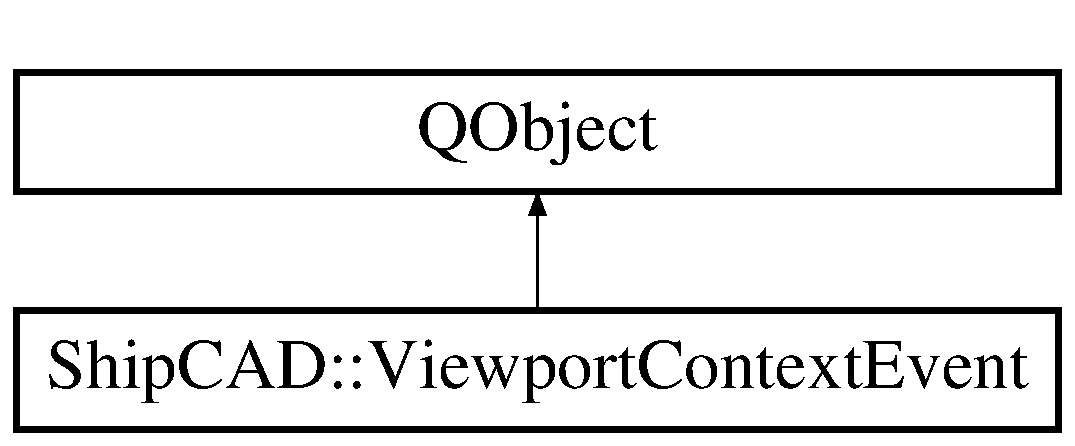
\includegraphics[height=2.000000cm]{classShipCAD_1_1ViewportContextEvent}
\end{center}
\end{figure}
\subsection*{Public Member Functions}
\begin{DoxyCompactItemize}
\item 
\hyperlink{classShipCAD_1_1ViewportContextEvent_a650e08d01b91eecaae90b3cd107ae46b}{Viewport\+Context\+Event} (\hyperlink{classShipCAD_1_1Viewport}{Viewport} $\ast$vp, Q\+Mouse\+Event $\ast$event)
\item 
\hyperlink{classShipCAD_1_1Viewport}{Viewport} $\ast$ \hyperlink{classShipCAD_1_1ViewportContextEvent_a1691135d434388eab7650f76dfb8c8f5}{get\+Viewport} ()
\item 
Q\+Mouse\+Event $\ast$ \hyperlink{classShipCAD_1_1ViewportContextEvent_aa0a673e4b6d86bf0235791827c29749e}{get\+Mouse\+Event} ()
\end{DoxyCompactItemize}


\subsection{Detailed Description}


Definition at line 54 of file viewport.\+h.



\subsection{Constructor \& Destructor Documentation}
\index{Ship\+C\+A\+D\+::\+Viewport\+Context\+Event@{Ship\+C\+A\+D\+::\+Viewport\+Context\+Event}!Viewport\+Context\+Event@{Viewport\+Context\+Event}}
\index{Viewport\+Context\+Event@{Viewport\+Context\+Event}!Ship\+C\+A\+D\+::\+Viewport\+Context\+Event@{Ship\+C\+A\+D\+::\+Viewport\+Context\+Event}}
\subsubsection[{\texorpdfstring{Viewport\+Context\+Event(\+Viewport $\ast$vp, Q\+Mouse\+Event $\ast$event)}{ViewportContextEvent(Viewport *vp, QMouseEvent *event)}}]{\setlength{\rightskip}{0pt plus 5cm}Viewport\+Context\+Event\+::\+Viewport\+Context\+Event (
\begin{DoxyParamCaption}
\item[{{\bf Viewport} $\ast$}]{vp, }
\item[{Q\+Mouse\+Event $\ast$}]{event}
\end{DoxyParamCaption}
)\hspace{0.3cm}{\ttfamily [explicit]}}\hypertarget{classShipCAD_1_1ViewportContextEvent_a650e08d01b91eecaae90b3cd107ae46b}{}\label{classShipCAD_1_1ViewportContextEvent_a650e08d01b91eecaae90b3cd107ae46b}


Definition at line 46 of file viewport.\+cpp.



\subsection{Member Function Documentation}
\index{Ship\+C\+A\+D\+::\+Viewport\+Context\+Event@{Ship\+C\+A\+D\+::\+Viewport\+Context\+Event}!get\+Mouse\+Event@{get\+Mouse\+Event}}
\index{get\+Mouse\+Event@{get\+Mouse\+Event}!Ship\+C\+A\+D\+::\+Viewport\+Context\+Event@{Ship\+C\+A\+D\+::\+Viewport\+Context\+Event}}
\subsubsection[{\texorpdfstring{get\+Mouse\+Event()}{getMouseEvent()}}]{\setlength{\rightskip}{0pt plus 5cm}Q\+Mouse\+Event$\ast$ Ship\+C\+A\+D\+::\+Viewport\+Context\+Event\+::get\+Mouse\+Event (
\begin{DoxyParamCaption}
{}
\end{DoxyParamCaption}
)\hspace{0.3cm}{\ttfamily [inline]}}\hypertarget{classShipCAD_1_1ViewportContextEvent_aa0a673e4b6d86bf0235791827c29749e}{}\label{classShipCAD_1_1ViewportContextEvent_aa0a673e4b6d86bf0235791827c29749e}


Definition at line 61 of file viewport.\+h.

\index{Ship\+C\+A\+D\+::\+Viewport\+Context\+Event@{Ship\+C\+A\+D\+::\+Viewport\+Context\+Event}!get\+Viewport@{get\+Viewport}}
\index{get\+Viewport@{get\+Viewport}!Ship\+C\+A\+D\+::\+Viewport\+Context\+Event@{Ship\+C\+A\+D\+::\+Viewport\+Context\+Event}}
\subsubsection[{\texorpdfstring{get\+Viewport()}{getViewport()}}]{\setlength{\rightskip}{0pt plus 5cm}{\bf Viewport}$\ast$ Ship\+C\+A\+D\+::\+Viewport\+Context\+Event\+::get\+Viewport (
\begin{DoxyParamCaption}
{}
\end{DoxyParamCaption}
)\hspace{0.3cm}{\ttfamily [inline]}}\hypertarget{classShipCAD_1_1ViewportContextEvent_a1691135d434388eab7650f76dfb8c8f5}{}\label{classShipCAD_1_1ViewportContextEvent_a1691135d434388eab7650f76dfb8c8f5}


Definition at line 60 of file viewport.\+h.



The documentation for this class was generated from the following files\+:\begin{DoxyCompactItemize}
\item 
Ship\+C\+A\+Dlib/\hyperlink{viewport_8h}{viewport.\+h}\item 
Ship\+C\+A\+Dlib/\hyperlink{viewport_8cpp}{viewport.\+cpp}\end{DoxyCompactItemize}

\hypertarget{classShipCAD_1_1ViewportView}{}\section{Ship\+C\+AD\+:\+:Viewport\+View Class Reference}
\label{classShipCAD_1_1ViewportView}\index{Ship\+C\+A\+D\+::\+Viewport\+View@{Ship\+C\+A\+D\+::\+Viewport\+View}}


Abstract class to calculate view, world matrices and operations using those for a viewport.  




{\ttfamily \#include $<$viewportview.\+h$>$}

Inheritance diagram for Ship\+C\+AD\+:\+:Viewport\+View\+:\begin{figure}[H]
\begin{center}
\leavevmode
\includegraphics[height=1.255605cm]{classShipCAD_1_1ViewportView}
\end{center}
\end{figure}
\subsection*{Public Member Functions}
\begin{DoxyCompactItemize}
\item 
\hyperlink{classShipCAD_1_1ViewportView_a725088d3f0e113c97ae52cccab7fce42}{Viewport\+View} (\hyperlink{classShipCAD_1_1Viewport}{Viewport} $\ast$vp)
\item 
virtual \hyperlink{classShipCAD_1_1ViewportView_a75f58efbb601f46ea20b70b1370cee1a}{$\sim$\+Viewport\+View} ()
\item 
virtual void \hyperlink{classShipCAD_1_1ViewportView_ab70e778772325a67610d983f630c2c3d}{reset\+View} ()
\item 
virtual void \hyperlink{classShipCAD_1_1ViewportView_ad1c89a6e34b7b3795a7f21e67181dc0f}{initialize\+Viewport} (const Q\+Vector3D \&min, const Q\+Vector3D \&max, int width, int height)=0
\item 
float \hyperlink{classShipCAD_1_1ViewportView_a69e218b17f56faac4fb02fec6ac9c5fb}{get\+Pick\+Dist} () const 
\item 
const Q\+Matrix4x4 \& \hyperlink{classShipCAD_1_1ViewportView_a0be1613b2ae2087da00811f2bdb0bd45}{get\+World} () const 
\item 
const Q\+Matrix4x4 \& \hyperlink{classShipCAD_1_1ViewportView_a6bffec9328b29bf40c868f2862daebe0}{get\+World\+Inv} () const 
\item 
const Q\+Matrix4x4 \& \hyperlink{classShipCAD_1_1ViewportView_af87bb73f78d5393d013708542eb184ae}{get\+Proj} () const 
\item 
const Q\+Matrix4x4 \& \hyperlink{classShipCAD_1_1ViewportView_a7e3e335818a369e64989f20d7a8dda4f}{get\+View} () const 
\item 
const Q\+Vector3D \& \hyperlink{classShipCAD_1_1ViewportView_a33150e3f757ddbbe045d7d046b4862e5}{get\+Camera} () const 
\item 
virtual bool \hyperlink{classShipCAD_1_1ViewportView_a4c2e113c5c0e58bb72576a8a802f5a29}{left\+Mouse\+Pick} (Q\+Point pos, int w, int h, \hyperlink{structShipCAD_1_1PickRay}{Pick\+Ray} \&ray)
\item 
virtual bool \hyperlink{classShipCAD_1_1ViewportView_a1e67e403d7307d3828336edbc1ded2f3}{right\+Mouse\+Pick} (Q\+Point pos, int w, int h)
\item 
virtual bool \hyperlink{classShipCAD_1_1ViewportView_ad74e96e8fef750466b2771f8fc48900a}{left\+Mouse\+Release} (Q\+Point pos, int w, int h)
\item 
virtual bool \hyperlink{classShipCAD_1_1ViewportView_aaeff27f9b32dc7ee98dbfc14b7eca804}{right\+Mouse\+Release} (Q\+Point pos, int w, int h)
\item 
virtual bool \hyperlink{classShipCAD_1_1ViewportView_a2dc46f8d032d707308cf853c70bc965a}{left\+Mouse\+Move} (Q\+Point cur, Q\+Point prev, int w, int h)
\item 
virtual bool \hyperlink{classShipCAD_1_1ViewportView_a44baf7aad8a3ba7ded04395a8765caf9}{middle\+Mouse\+Move} (Q\+Point cur, Q\+Point prev, int w, int h)
\item 
virtual bool \hyperlink{classShipCAD_1_1ViewportView_a537210f7c2872e7b8921341660e85347}{right\+Mouse\+Move} (Q\+Point cur, Q\+Point prev, int w, int h)
\item 
virtual bool \hyperlink{classShipCAD_1_1ViewportView_a77ce1c6a0216a791ee2ae79dd6674cde}{wheel\+With\+Degrees} (Q\+Point degrees, int w, int h)
\item 
Q\+Point \hyperlink{classShipCAD_1_1ViewportView_ac763be6de52b393cb0b9ff4be4c66fcf}{convert3D} (const Q\+Vector3D \&pt, int w, int h) const 
\begin{DoxyCompactList}\small\item\em convert a 3D point to viewport 2d coordinates \end{DoxyCompactList}\item 
virtual Q\+Vector2D \hyperlink{classShipCAD_1_1ViewportView_a2bc94791273d6134566a386f2a735e37}{project\+To3D} (Q\+Point pos, int w, int h)=0
\begin{DoxyCompactList}\small\item\em convert screen coordinates to 2D world coordinates \end{DoxyCompactList}\item 
virtual bool \hyperlink{classShipCAD_1_1ViewportView_a6991b6b121b609ec7d18518a8f872859}{point\+Drag} (Q\+Point pos, int w, int h, Q\+Vector3D \&newcoord)
\begin{DoxyCompactList}\small\item\em drag a point in the viewport \end{DoxyCompactList}\item 
virtual \hyperlink{structShipCAD_1_1PickRay}{Pick\+Ray} \hyperlink{classShipCAD_1_1ViewportView_a845fc1fe9fa6ec52726fba1ad350e638}{convert\+Mouse\+Coord\+To\+World} (Q\+Point pos, int width, int height) const 
\begin{DoxyCompactList}\small\item\em given mouse coordinates, find a pick ray for this view \end{DoxyCompactList}\end{DoxyCompactItemize}
\subsection*{Static Public Member Functions}
\begin{DoxyCompactItemize}
\item 
static \hyperlink{classShipCAD_1_1ViewportView}{Viewport\+View} $\ast$ \hyperlink{classShipCAD_1_1ViewportView_aec2ef49c2d2ecf9099dfbf32cd645144}{construct} (\hyperlink{namespaceShipCAD_aeeeb05810f2e31ef89fd4ac6b6ba9c0a}{viewport\+\_\+type\+\_\+t} ty, \hyperlink{classShipCAD_1_1Viewport}{Viewport} $\ast$vp)
\end{DoxyCompactItemize}
\subsection*{Protected Member Functions}
\begin{DoxyCompactItemize}
\item 
virtual void \hyperlink{classShipCAD_1_1ViewportView_a15b8dab8f55b9967feeb7b93c234053d}{finish\+Setup} ()
\end{DoxyCompactItemize}
\subsection*{Protected Attributes}
\begin{DoxyCompactItemize}
\item 
\hyperlink{classShipCAD_1_1Viewport}{Viewport} $\ast$ \hyperlink{classShipCAD_1_1ViewportView_a9d980ea46c1638d05221dc71e666da04}{\+\_\+vp}
\item 
float \hyperlink{classShipCAD_1_1ViewportView_a337e90ffddd63535bad9b8de652a455a}{\+\_\+zoom}
\item 
float \hyperlink{classShipCAD_1_1ViewportView_a3cccfb1058f0c8f66d662c1f19ed5c33}{\+\_\+panX}
\item 
float \hyperlink{classShipCAD_1_1ViewportView_aa2a8062a009ea1a9f26498a103134d3f}{\+\_\+panY}
\item 
float \hyperlink{classShipCAD_1_1ViewportView_a808cc636969188f7c04c97902ecbe9d5}{\+\_\+scale}
\item 
float \hyperlink{classShipCAD_1_1ViewportView_a4cce24be9f8367c04714cd5f091ad637}{\+\_\+margin}
\item 
float \hyperlink{classShipCAD_1_1ViewportView_a001cda888a20319d4d3b29bd9926d5e1}{\+\_\+pick\+Dist}
\item 
Q\+Vector3D \hyperlink{classShipCAD_1_1ViewportView_af4017af3ac64751ce2c5f348d2567657}{\+\_\+midpoint}
\item 
Q\+Vector3D \hyperlink{classShipCAD_1_1ViewportView_ac357a478169de078d3dc3289a15612b1}{\+\_\+camera\+\_\+location}
\item 
Q\+Matrix4x4 \hyperlink{classShipCAD_1_1ViewportView_a1b2d9753e22af2e9a071e60799478905}{\+\_\+world}
\item 
Q\+Matrix4x4 \hyperlink{classShipCAD_1_1ViewportView_a6b16d2dd6a5c1b812e9fa96dfcadebbb}{\+\_\+world\+Inv}
\item 
Q\+Matrix4x4 \hyperlink{classShipCAD_1_1ViewportView_a56588119357f01d0764219252695e9c5}{\+\_\+view}
\item 
Q\+Matrix4x4 \hyperlink{classShipCAD_1_1ViewportView_abb5933e4e5cbe5c97be2b63164cc8380}{\+\_\+proj}
\item 
Q\+Vector3D \hyperlink{classShipCAD_1_1ViewportView_af523ce78903a7c9b9d1c2e5548d8a283}{\+\_\+max}
\item 
Q\+Vector3D \hyperlink{classShipCAD_1_1ViewportView_a8d957ad40e793a09f4741200eec4a939}{\+\_\+min}
\end{DoxyCompactItemize}


\subsection{Detailed Description}
Abstract class to calculate view, world matrices and operations using those for a viewport. 

Definition at line 46 of file viewportview.\+h.



\subsection{Constructor \& Destructor Documentation}
\index{Ship\+C\+A\+D\+::\+Viewport\+View@{Ship\+C\+A\+D\+::\+Viewport\+View}!Viewport\+View@{Viewport\+View}}
\index{Viewport\+View@{Viewport\+View}!Ship\+C\+A\+D\+::\+Viewport\+View@{Ship\+C\+A\+D\+::\+Viewport\+View}}
\subsubsection[{\texorpdfstring{Viewport\+View(\+Viewport $\ast$vp)}{ViewportView(Viewport *vp)}}]{\setlength{\rightskip}{0pt plus 5cm}Viewport\+View\+::\+Viewport\+View (
\begin{DoxyParamCaption}
\item[{{\bf Viewport} $\ast$}]{vp}
\end{DoxyParamCaption}
)\hspace{0.3cm}{\ttfamily [explicit]}}\hypertarget{classShipCAD_1_1ViewportView_a725088d3f0e113c97ae52cccab7fce42}{}\label{classShipCAD_1_1ViewportView_a725088d3f0e113c97ae52cccab7fce42}


Definition at line 45 of file viewportview.\+cpp.

\index{Ship\+C\+A\+D\+::\+Viewport\+View@{Ship\+C\+A\+D\+::\+Viewport\+View}!````~Viewport\+View@{$\sim$\+Viewport\+View}}
\index{````~Viewport\+View@{$\sim$\+Viewport\+View}!Ship\+C\+A\+D\+::\+Viewport\+View@{Ship\+C\+A\+D\+::\+Viewport\+View}}
\subsubsection[{\texorpdfstring{$\sim$\+Viewport\+View()}{~ViewportView()}}]{\setlength{\rightskip}{0pt plus 5cm}virtual Ship\+C\+A\+D\+::\+Viewport\+View\+::$\sim$\+Viewport\+View (
\begin{DoxyParamCaption}
{}
\end{DoxyParamCaption}
)\hspace{0.3cm}{\ttfamily [inline]}, {\ttfamily [virtual]}}\hypertarget{classShipCAD_1_1ViewportView_a75f58efbb601f46ea20b70b1370cee1a}{}\label{classShipCAD_1_1ViewportView_a75f58efbb601f46ea20b70b1370cee1a}


Definition at line 51 of file viewportview.\+h.



\subsection{Member Function Documentation}
\index{Ship\+C\+A\+D\+::\+Viewport\+View@{Ship\+C\+A\+D\+::\+Viewport\+View}!construct@{construct}}
\index{construct@{construct}!Ship\+C\+A\+D\+::\+Viewport\+View@{Ship\+C\+A\+D\+::\+Viewport\+View}}
\subsubsection[{\texorpdfstring{construct(viewport\+\_\+type\+\_\+t ty, Viewport $\ast$vp)}{construct(viewport_type_t ty, Viewport *vp)}}]{\setlength{\rightskip}{0pt plus 5cm}{\bf Viewport\+View} $\ast$ Viewport\+View\+::construct (
\begin{DoxyParamCaption}
\item[{{\bf viewport\+\_\+type\+\_\+t}}]{ty, }
\item[{{\bf Viewport} $\ast$}]{vp}
\end{DoxyParamCaption}
)\hspace{0.3cm}{\ttfamily [static]}}\hypertarget{classShipCAD_1_1ViewportView_aec2ef49c2d2ecf9099dfbf32cd645144}{}\label{classShipCAD_1_1ViewportView_aec2ef49c2d2ecf9099dfbf32cd645144}


Definition at line 52 of file viewportview.\+cpp.

\index{Ship\+C\+A\+D\+::\+Viewport\+View@{Ship\+C\+A\+D\+::\+Viewport\+View}!convert3D@{convert3D}}
\index{convert3D@{convert3D}!Ship\+C\+A\+D\+::\+Viewport\+View@{Ship\+C\+A\+D\+::\+Viewport\+View}}
\subsubsection[{\texorpdfstring{convert3\+D(const Q\+Vector3\+D \&pt, int w, int h) const }{convert3D(const QVector3D &pt, int w, int h) const }}]{\setlength{\rightskip}{0pt plus 5cm}Q\+Point Viewport\+View\+::convert3D (
\begin{DoxyParamCaption}
\item[{const Q\+Vector3D \&}]{pt, }
\item[{int}]{w, }
\item[{int}]{h}
\end{DoxyParamCaption}
) const}\hypertarget{classShipCAD_1_1ViewportView_ac763be6de52b393cb0b9ff4be4c66fcf}{}\label{classShipCAD_1_1ViewportView_ac763be6de52b393cb0b9ff4be4c66fcf}


convert a 3D point to viewport 2d coordinates 


\begin{DoxyParams}{Parameters}
{\em pt} & the 3D point to convert \\
\hline
{\em w} & width of viewport in pixels \\
\hline
{\em h} & height of viewport in pixels \\
\hline
\end{DoxyParams}
\begin{DoxyReturn}{Returns}
point in x, y coordinates with 0,0 upper left corner of viewport 
\end{DoxyReturn}


Definition at line 86 of file viewportview.\+cpp.

\index{Ship\+C\+A\+D\+::\+Viewport\+View@{Ship\+C\+A\+D\+::\+Viewport\+View}!convert\+Mouse\+Coord\+To\+World@{convert\+Mouse\+Coord\+To\+World}}
\index{convert\+Mouse\+Coord\+To\+World@{convert\+Mouse\+Coord\+To\+World}!Ship\+C\+A\+D\+::\+Viewport\+View@{Ship\+C\+A\+D\+::\+Viewport\+View}}
\subsubsection[{\texorpdfstring{convert\+Mouse\+Coord\+To\+World(\+Q\+Point pos, int width, int height) const }{convertMouseCoordToWorld(QPoint pos, int width, int height) const }}]{\setlength{\rightskip}{0pt plus 5cm}{\bf Ship\+C\+A\+D\+::\+Pick\+Ray} Viewport\+View\+::convert\+Mouse\+Coord\+To\+World (
\begin{DoxyParamCaption}
\item[{Q\+Point}]{pos, }
\item[{int}]{width, }
\item[{int}]{height}
\end{DoxyParamCaption}
) const\hspace{0.3cm}{\ttfamily [virtual]}}\hypertarget{classShipCAD_1_1ViewportView_a845fc1fe9fa6ec52726fba1ad350e638}{}\label{classShipCAD_1_1ViewportView_a845fc1fe9fa6ec52726fba1ad350e638}


given mouse coordinates, find a pick ray for this view 


\begin{DoxyParams}{Parameters}
{\em pos} & the mouse coordinates \\
\hline
{\em width} & the viewport width in pixels \\
\hline
{\em height} & the viewport height in pixels \\
\hline
\end{DoxyParams}
\begin{DoxyReturn}{Returns}
the world coordinate system \hyperlink{structShipCAD_1_1PickRay}{Pick\+Ray} corresponding to the mouse coordinates 
\end{DoxyReturn}


Definition at line 154 of file viewportview.\+cpp.

\index{Ship\+C\+A\+D\+::\+Viewport\+View@{Ship\+C\+A\+D\+::\+Viewport\+View}!finish\+Setup@{finish\+Setup}}
\index{finish\+Setup@{finish\+Setup}!Ship\+C\+A\+D\+::\+Viewport\+View@{Ship\+C\+A\+D\+::\+Viewport\+View}}
\subsubsection[{\texorpdfstring{finish\+Setup()}{finishSetup()}}]{\setlength{\rightskip}{0pt plus 5cm}void Viewport\+View\+::finish\+Setup (
\begin{DoxyParamCaption}
{}
\end{DoxyParamCaption}
)\hspace{0.3cm}{\ttfamily [protected]}, {\ttfamily [virtual]}}\hypertarget{classShipCAD_1_1ViewportView_a15b8dab8f55b9967feeb7b93c234053d}{}\label{classShipCAD_1_1ViewportView_a15b8dab8f55b9967feeb7b93c234053d}


Definition at line 66 of file viewportview.\+cpp.

\index{Ship\+C\+A\+D\+::\+Viewport\+View@{Ship\+C\+A\+D\+::\+Viewport\+View}!get\+Camera@{get\+Camera}}
\index{get\+Camera@{get\+Camera}!Ship\+C\+A\+D\+::\+Viewport\+View@{Ship\+C\+A\+D\+::\+Viewport\+View}}
\subsubsection[{\texorpdfstring{get\+Camera() const }{getCamera() const }}]{\setlength{\rightskip}{0pt plus 5cm}const Q\+Vector3D\& Ship\+C\+A\+D\+::\+Viewport\+View\+::get\+Camera (
\begin{DoxyParamCaption}
{}
\end{DoxyParamCaption}
) const\hspace{0.3cm}{\ttfamily [inline]}}\hypertarget{classShipCAD_1_1ViewportView_a33150e3f757ddbbe045d7d046b4862e5}{}\label{classShipCAD_1_1ViewportView_a33150e3f757ddbbe045d7d046b4862e5}


Definition at line 69 of file viewportview.\+h.

\index{Ship\+C\+A\+D\+::\+Viewport\+View@{Ship\+C\+A\+D\+::\+Viewport\+View}!get\+Pick\+Dist@{get\+Pick\+Dist}}
\index{get\+Pick\+Dist@{get\+Pick\+Dist}!Ship\+C\+A\+D\+::\+Viewport\+View@{Ship\+C\+A\+D\+::\+Viewport\+View}}
\subsubsection[{\texorpdfstring{get\+Pick\+Dist() const }{getPickDist() const }}]{\setlength{\rightskip}{0pt plus 5cm}float Ship\+C\+A\+D\+::\+Viewport\+View\+::get\+Pick\+Dist (
\begin{DoxyParamCaption}
{}
\end{DoxyParamCaption}
) const\hspace{0.3cm}{\ttfamily [inline]}}\hypertarget{classShipCAD_1_1ViewportView_a69e218b17f56faac4fb02fec6ac9c5fb}{}\label{classShipCAD_1_1ViewportView_a69e218b17f56faac4fb02fec6ac9c5fb}


Definition at line 59 of file viewportview.\+h.

\index{Ship\+C\+A\+D\+::\+Viewport\+View@{Ship\+C\+A\+D\+::\+Viewport\+View}!get\+Proj@{get\+Proj}}
\index{get\+Proj@{get\+Proj}!Ship\+C\+A\+D\+::\+Viewport\+View@{Ship\+C\+A\+D\+::\+Viewport\+View}}
\subsubsection[{\texorpdfstring{get\+Proj() const }{getProj() const }}]{\setlength{\rightskip}{0pt plus 5cm}const Q\+Matrix4x4\& Ship\+C\+A\+D\+::\+Viewport\+View\+::get\+Proj (
\begin{DoxyParamCaption}
{}
\end{DoxyParamCaption}
) const\hspace{0.3cm}{\ttfamily [inline]}}\hypertarget{classShipCAD_1_1ViewportView_af87bb73f78d5393d013708542eb184ae}{}\label{classShipCAD_1_1ViewportView_af87bb73f78d5393d013708542eb184ae}


Definition at line 65 of file viewportview.\+h.

\index{Ship\+C\+A\+D\+::\+Viewport\+View@{Ship\+C\+A\+D\+::\+Viewport\+View}!get\+View@{get\+View}}
\index{get\+View@{get\+View}!Ship\+C\+A\+D\+::\+Viewport\+View@{Ship\+C\+A\+D\+::\+Viewport\+View}}
\subsubsection[{\texorpdfstring{get\+View() const }{getView() const }}]{\setlength{\rightskip}{0pt plus 5cm}const Q\+Matrix4x4\& Ship\+C\+A\+D\+::\+Viewport\+View\+::get\+View (
\begin{DoxyParamCaption}
{}
\end{DoxyParamCaption}
) const\hspace{0.3cm}{\ttfamily [inline]}}\hypertarget{classShipCAD_1_1ViewportView_a7e3e335818a369e64989f20d7a8dda4f}{}\label{classShipCAD_1_1ViewportView_a7e3e335818a369e64989f20d7a8dda4f}


Definition at line 67 of file viewportview.\+h.

\index{Ship\+C\+A\+D\+::\+Viewport\+View@{Ship\+C\+A\+D\+::\+Viewport\+View}!get\+World@{get\+World}}
\index{get\+World@{get\+World}!Ship\+C\+A\+D\+::\+Viewport\+View@{Ship\+C\+A\+D\+::\+Viewport\+View}}
\subsubsection[{\texorpdfstring{get\+World() const }{getWorld() const }}]{\setlength{\rightskip}{0pt plus 5cm}const Q\+Matrix4x4\& Ship\+C\+A\+D\+::\+Viewport\+View\+::get\+World (
\begin{DoxyParamCaption}
{}
\end{DoxyParamCaption}
) const\hspace{0.3cm}{\ttfamily [inline]}}\hypertarget{classShipCAD_1_1ViewportView_a0be1613b2ae2087da00811f2bdb0bd45}{}\label{classShipCAD_1_1ViewportView_a0be1613b2ae2087da00811f2bdb0bd45}


Definition at line 61 of file viewportview.\+h.

\index{Ship\+C\+A\+D\+::\+Viewport\+View@{Ship\+C\+A\+D\+::\+Viewport\+View}!get\+World\+Inv@{get\+World\+Inv}}
\index{get\+World\+Inv@{get\+World\+Inv}!Ship\+C\+A\+D\+::\+Viewport\+View@{Ship\+C\+A\+D\+::\+Viewport\+View}}
\subsubsection[{\texorpdfstring{get\+World\+Inv() const }{getWorldInv() const }}]{\setlength{\rightskip}{0pt plus 5cm}const Q\+Matrix4x4\& Ship\+C\+A\+D\+::\+Viewport\+View\+::get\+World\+Inv (
\begin{DoxyParamCaption}
{}
\end{DoxyParamCaption}
) const\hspace{0.3cm}{\ttfamily [inline]}}\hypertarget{classShipCAD_1_1ViewportView_a6bffec9328b29bf40c868f2862daebe0}{}\label{classShipCAD_1_1ViewportView_a6bffec9328b29bf40c868f2862daebe0}


Definition at line 63 of file viewportview.\+h.

\index{Ship\+C\+A\+D\+::\+Viewport\+View@{Ship\+C\+A\+D\+::\+Viewport\+View}!initialize\+Viewport@{initialize\+Viewport}}
\index{initialize\+Viewport@{initialize\+Viewport}!Ship\+C\+A\+D\+::\+Viewport\+View@{Ship\+C\+A\+D\+::\+Viewport\+View}}
\subsubsection[{\texorpdfstring{initialize\+Viewport(const Q\+Vector3\+D \&min, const Q\+Vector3\+D \&max, int width, int height)=0}{initializeViewport(const QVector3D &min, const QVector3D &max, int width, int height)=0}}]{\setlength{\rightskip}{0pt plus 5cm}virtual void Ship\+C\+A\+D\+::\+Viewport\+View\+::initialize\+Viewport (
\begin{DoxyParamCaption}
\item[{const Q\+Vector3D \&}]{min, }
\item[{const Q\+Vector3D \&}]{max, }
\item[{int}]{width, }
\item[{int}]{height}
\end{DoxyParamCaption}
)\hspace{0.3cm}{\ttfamily [pure virtual]}}\hypertarget{classShipCAD_1_1ViewportView_ad1c89a6e34b7b3795a7f21e67181dc0f}{}\label{classShipCAD_1_1ViewportView_ad1c89a6e34b7b3795a7f21e67181dc0f}


Implemented in \hyperlink{classShipCAD_1_1ViewportViewBodyplan_aaa33b893fbff1c2899d5779fc3b78d1e}{Ship\+C\+A\+D\+::\+Viewport\+View\+Bodyplan}, \hyperlink{classShipCAD_1_1ViewportViewProfile_ae8ac602b7c67fddbfce7ceeda85676b3}{Ship\+C\+A\+D\+::\+Viewport\+View\+Profile}, \hyperlink{classShipCAD_1_1ViewportViewPlan_a05836d5f48d28a0681a1a3214dc4aeac}{Ship\+C\+A\+D\+::\+Viewport\+View\+Plan}, and \hyperlink{classShipCAD_1_1ViewportViewPerspective_af96ca2b448d261206e360b1304510a65}{Ship\+C\+A\+D\+::\+Viewport\+View\+Perspective}.

\index{Ship\+C\+A\+D\+::\+Viewport\+View@{Ship\+C\+A\+D\+::\+Viewport\+View}!left\+Mouse\+Move@{left\+Mouse\+Move}}
\index{left\+Mouse\+Move@{left\+Mouse\+Move}!Ship\+C\+A\+D\+::\+Viewport\+View@{Ship\+C\+A\+D\+::\+Viewport\+View}}
\subsubsection[{\texorpdfstring{left\+Mouse\+Move(\+Q\+Point cur, Q\+Point prev, int w, int h)}{leftMouseMove(QPoint cur, QPoint prev, int w, int h)}}]{\setlength{\rightskip}{0pt plus 5cm}bool Viewport\+View\+::left\+Mouse\+Move (
\begin{DoxyParamCaption}
\item[{Q\+Point}]{cur, }
\item[{Q\+Point}]{prev, }
\item[{int}]{w, }
\item[{int}]{h}
\end{DoxyParamCaption}
)\hspace{0.3cm}{\ttfamily [virtual]}}\hypertarget{classShipCAD_1_1ViewportView_a2dc46f8d032d707308cf853c70bc965a}{}\label{classShipCAD_1_1ViewportView_a2dc46f8d032d707308cf853c70bc965a}


Reimplemented in \hyperlink{classShipCAD_1_1ViewportViewPerspective_a11f5f04a95646a701743804c4d7c1d10}{Ship\+C\+A\+D\+::\+Viewport\+View\+Perspective}.



Definition at line 125 of file viewportview.\+cpp.

\index{Ship\+C\+A\+D\+::\+Viewport\+View@{Ship\+C\+A\+D\+::\+Viewport\+View}!left\+Mouse\+Pick@{left\+Mouse\+Pick}}
\index{left\+Mouse\+Pick@{left\+Mouse\+Pick}!Ship\+C\+A\+D\+::\+Viewport\+View@{Ship\+C\+A\+D\+::\+Viewport\+View}}
\subsubsection[{\texorpdfstring{left\+Mouse\+Pick(\+Q\+Point pos, int w, int h, Pick\+Ray \&ray)}{leftMousePick(QPoint pos, int w, int h, PickRay &ray)}}]{\setlength{\rightskip}{0pt plus 5cm}bool Viewport\+View\+::left\+Mouse\+Pick (
\begin{DoxyParamCaption}
\item[{Q\+Point}]{pos, }
\item[{int}]{w, }
\item[{int}]{h, }
\item[{{\bf Pick\+Ray} \&}]{ray}
\end{DoxyParamCaption}
)\hspace{0.3cm}{\ttfamily [virtual]}}\hypertarget{classShipCAD_1_1ViewportView_a4c2e113c5c0e58bb72576a8a802f5a29}{}\label{classShipCAD_1_1ViewportView_a4c2e113c5c0e58bb72576a8a802f5a29}


Definition at line 92 of file viewportview.\+cpp.

\index{Ship\+C\+A\+D\+::\+Viewport\+View@{Ship\+C\+A\+D\+::\+Viewport\+View}!left\+Mouse\+Release@{left\+Mouse\+Release}}
\index{left\+Mouse\+Release@{left\+Mouse\+Release}!Ship\+C\+A\+D\+::\+Viewport\+View@{Ship\+C\+A\+D\+::\+Viewport\+View}}
\subsubsection[{\texorpdfstring{left\+Mouse\+Release(\+Q\+Point pos, int w, int h)}{leftMouseRelease(QPoint pos, int w, int h)}}]{\setlength{\rightskip}{0pt plus 5cm}bool Viewport\+View\+::left\+Mouse\+Release (
\begin{DoxyParamCaption}
\item[{Q\+Point}]{pos, }
\item[{int}]{w, }
\item[{int}]{h}
\end{DoxyParamCaption}
)\hspace{0.3cm}{\ttfamily [virtual]}}\hypertarget{classShipCAD_1_1ViewportView_ad74e96e8fef750466b2771f8fc48900a}{}\label{classShipCAD_1_1ViewportView_ad74e96e8fef750466b2771f8fc48900a}


Definition at line 108 of file viewportview.\+cpp.

\index{Ship\+C\+A\+D\+::\+Viewport\+View@{Ship\+C\+A\+D\+::\+Viewport\+View}!middle\+Mouse\+Move@{middle\+Mouse\+Move}}
\index{middle\+Mouse\+Move@{middle\+Mouse\+Move}!Ship\+C\+A\+D\+::\+Viewport\+View@{Ship\+C\+A\+D\+::\+Viewport\+View}}
\subsubsection[{\texorpdfstring{middle\+Mouse\+Move(\+Q\+Point cur, Q\+Point prev, int w, int h)}{middleMouseMove(QPoint cur, QPoint prev, int w, int h)}}]{\setlength{\rightskip}{0pt plus 5cm}bool Viewport\+View\+::middle\+Mouse\+Move (
\begin{DoxyParamCaption}
\item[{Q\+Point}]{cur, }
\item[{Q\+Point}]{prev, }
\item[{int}]{w, }
\item[{int}]{h}
\end{DoxyParamCaption}
)\hspace{0.3cm}{\ttfamily [virtual]}}\hypertarget{classShipCAD_1_1ViewportView_a44baf7aad8a3ba7ded04395a8765caf9}{}\label{classShipCAD_1_1ViewportView_a44baf7aad8a3ba7ded04395a8765caf9}


Reimplemented in \hyperlink{classShipCAD_1_1ViewportViewPerspective_a1de2fd402609b54c79c2d70390ba4a64}{Ship\+C\+A\+D\+::\+Viewport\+View\+Perspective}.



Definition at line 120 of file viewportview.\+cpp.

\index{Ship\+C\+A\+D\+::\+Viewport\+View@{Ship\+C\+A\+D\+::\+Viewport\+View}!point\+Drag@{point\+Drag}}
\index{point\+Drag@{point\+Drag}!Ship\+C\+A\+D\+::\+Viewport\+View@{Ship\+C\+A\+D\+::\+Viewport\+View}}
\subsubsection[{\texorpdfstring{point\+Drag(\+Q\+Point pos, int w, int h, Q\+Vector3\+D \&newcoord)}{pointDrag(QPoint pos, int w, int h, QVector3D &newcoord)}}]{\setlength{\rightskip}{0pt plus 5cm}bool Viewport\+View\+::point\+Drag (
\begin{DoxyParamCaption}
\item[{Q\+Point}]{pos, }
\item[{int}]{w, }
\item[{int}]{h, }
\item[{Q\+Vector3D \&}]{newcoord}
\end{DoxyParamCaption}
)\hspace{0.3cm}{\ttfamily [virtual]}}\hypertarget{classShipCAD_1_1ViewportView_a6991b6b121b609ec7d18518a8f872859}{}\label{classShipCAD_1_1ViewportView_a6991b6b121b609ec7d18518a8f872859}


drag a point in the viewport 


\begin{DoxyParams}{Parameters}
{\em pos} & the current mouse coordinates \\
\hline
{\em w} & width of viewport in pixels \\
\hline
{\em h} & height of viewport in pixels \\
\hline
{\em newcoord} & the new coordinates of the point in 3D space \\
\hline
\end{DoxyParams}
\begin{DoxyReturn}{Returns}
true if the point can be dragged in this view 
\end{DoxyReturn}


Reimplemented in \hyperlink{classShipCAD_1_1ViewportViewBodyplan_af10d2ce23c6634a6f5824e49f678998b}{Ship\+C\+A\+D\+::\+Viewport\+View\+Bodyplan}, \hyperlink{classShipCAD_1_1ViewportViewProfile_abc8adc37b3539da20124a9d1930cfc92}{Ship\+C\+A\+D\+::\+Viewport\+View\+Profile}, and \hyperlink{classShipCAD_1_1ViewportViewPlan_aaac7978a626640198a7a92daae63bc51}{Ship\+C\+A\+D\+::\+Viewport\+View\+Plan}.



Definition at line 149 of file viewportview.\+cpp.

\index{Ship\+C\+A\+D\+::\+Viewport\+View@{Ship\+C\+A\+D\+::\+Viewport\+View}!project\+To3D@{project\+To3D}}
\index{project\+To3D@{project\+To3D}!Ship\+C\+A\+D\+::\+Viewport\+View@{Ship\+C\+A\+D\+::\+Viewport\+View}}
\subsubsection[{\texorpdfstring{project\+To3\+D(\+Q\+Point pos, int w, int h)=0}{projectTo3D(QPoint pos, int w, int h)=0}}]{\setlength{\rightskip}{0pt plus 5cm}virtual Q\+Vector2D Ship\+C\+A\+D\+::\+Viewport\+View\+::project\+To3D (
\begin{DoxyParamCaption}
\item[{Q\+Point}]{pos, }
\item[{int}]{w, }
\item[{int}]{h}
\end{DoxyParamCaption}
)\hspace{0.3cm}{\ttfamily [pure virtual]}}\hypertarget{classShipCAD_1_1ViewportView_a2bc94791273d6134566a386f2a735e37}{}\label{classShipCAD_1_1ViewportView_a2bc94791273d6134566a386f2a735e37}


convert screen coordinates to 2D world coordinates 


\begin{DoxyParams}{Parameters}
{\em pos} & screen position \\
\hline
{\em w} & width of viewport in pixels \\
\hline
{\em h} & height of viewport in pixels \\
\hline
\end{DoxyParams}
\begin{DoxyReturn}{Returns}
the world coordinates of screen position 
\end{DoxyReturn}


Implemented in \hyperlink{classShipCAD_1_1ViewportViewBodyplan_a919c765ec9749814bac1ef0a3b3e8ef1}{Ship\+C\+A\+D\+::\+Viewport\+View\+Bodyplan}, \hyperlink{classShipCAD_1_1ViewportViewProfile_a6158e95a906d0b62064e72ead2263a73}{Ship\+C\+A\+D\+::\+Viewport\+View\+Profile}, \hyperlink{classShipCAD_1_1ViewportViewPlan_adcc5e44591098694df045848798be804}{Ship\+C\+A\+D\+::\+Viewport\+View\+Plan}, and \hyperlink{classShipCAD_1_1ViewportViewPerspective_afc402aace76462bb3b0431cebba6a6a5}{Ship\+C\+A\+D\+::\+Viewport\+View\+Perspective}.

\index{Ship\+C\+A\+D\+::\+Viewport\+View@{Ship\+C\+A\+D\+::\+Viewport\+View}!reset\+View@{reset\+View}}
\index{reset\+View@{reset\+View}!Ship\+C\+A\+D\+::\+Viewport\+View@{Ship\+C\+A\+D\+::\+Viewport\+View}}
\subsubsection[{\texorpdfstring{reset\+View()}{resetView()}}]{\setlength{\rightskip}{0pt plus 5cm}void Viewport\+View\+::reset\+View (
\begin{DoxyParamCaption}
{}
\end{DoxyParamCaption}
)\hspace{0.3cm}{\ttfamily [virtual]}}\hypertarget{classShipCAD_1_1ViewportView_ab70e778772325a67610d983f630c2c3d}{}\label{classShipCAD_1_1ViewportView_ab70e778772325a67610d983f630c2c3d}


Reimplemented in \hyperlink{classShipCAD_1_1ViewportViewPerspective_ab3cc69a6cdb3271cc9e79ec16aa37a33}{Ship\+C\+A\+D\+::\+Viewport\+View\+Perspective}.



Definition at line 78 of file viewportview.\+cpp.

\index{Ship\+C\+A\+D\+::\+Viewport\+View@{Ship\+C\+A\+D\+::\+Viewport\+View}!right\+Mouse\+Move@{right\+Mouse\+Move}}
\index{right\+Mouse\+Move@{right\+Mouse\+Move}!Ship\+C\+A\+D\+::\+Viewport\+View@{Ship\+C\+A\+D\+::\+Viewport\+View}}
\subsubsection[{\texorpdfstring{right\+Mouse\+Move(\+Q\+Point cur, Q\+Point prev, int w, int h)}{rightMouseMove(QPoint cur, QPoint prev, int w, int h)}}]{\setlength{\rightskip}{0pt plus 5cm}bool Viewport\+View\+::right\+Mouse\+Move (
\begin{DoxyParamCaption}
\item[{Q\+Point}]{cur, }
\item[{Q\+Point}]{prev, }
\item[{int}]{w, }
\item[{int}]{h}
\end{DoxyParamCaption}
)\hspace{0.3cm}{\ttfamily [virtual]}}\hypertarget{classShipCAD_1_1ViewportView_a537210f7c2872e7b8921341660e85347}{}\label{classShipCAD_1_1ViewportView_a537210f7c2872e7b8921341660e85347}


Reimplemented in \hyperlink{classShipCAD_1_1ViewportViewBodyplan_acbc25d95fff9310b5cf5cfa1c5dd5210}{Ship\+C\+A\+D\+::\+Viewport\+View\+Bodyplan}, \hyperlink{classShipCAD_1_1ViewportViewProfile_a8fccdc2ff4cb6021b6e810712d45b8f0}{Ship\+C\+A\+D\+::\+Viewport\+View\+Profile}, and \hyperlink{classShipCAD_1_1ViewportViewPlan_a932d06d121e39a91676053c667fc78d5}{Ship\+C\+A\+D\+::\+Viewport\+View\+Plan}.



Definition at line 130 of file viewportview.\+cpp.

\index{Ship\+C\+A\+D\+::\+Viewport\+View@{Ship\+C\+A\+D\+::\+Viewport\+View}!right\+Mouse\+Pick@{right\+Mouse\+Pick}}
\index{right\+Mouse\+Pick@{right\+Mouse\+Pick}!Ship\+C\+A\+D\+::\+Viewport\+View@{Ship\+C\+A\+D\+::\+Viewport\+View}}
\subsubsection[{\texorpdfstring{right\+Mouse\+Pick(\+Q\+Point pos, int w, int h)}{rightMousePick(QPoint pos, int w, int h)}}]{\setlength{\rightskip}{0pt plus 5cm}bool Viewport\+View\+::right\+Mouse\+Pick (
\begin{DoxyParamCaption}
\item[{Q\+Point}]{pos, }
\item[{int}]{w, }
\item[{int}]{h}
\end{DoxyParamCaption}
)\hspace{0.3cm}{\ttfamily [virtual]}}\hypertarget{classShipCAD_1_1ViewportView_a1e67e403d7307d3828336edbc1ded2f3}{}\label{classShipCAD_1_1ViewportView_a1e67e403d7307d3828336edbc1ded2f3}


Definition at line 103 of file viewportview.\+cpp.

\index{Ship\+C\+A\+D\+::\+Viewport\+View@{Ship\+C\+A\+D\+::\+Viewport\+View}!right\+Mouse\+Release@{right\+Mouse\+Release}}
\index{right\+Mouse\+Release@{right\+Mouse\+Release}!Ship\+C\+A\+D\+::\+Viewport\+View@{Ship\+C\+A\+D\+::\+Viewport\+View}}
\subsubsection[{\texorpdfstring{right\+Mouse\+Release(\+Q\+Point pos, int w, int h)}{rightMouseRelease(QPoint pos, int w, int h)}}]{\setlength{\rightskip}{0pt plus 5cm}bool Viewport\+View\+::right\+Mouse\+Release (
\begin{DoxyParamCaption}
\item[{Q\+Point}]{pos, }
\item[{int}]{w, }
\item[{int}]{h}
\end{DoxyParamCaption}
)\hspace{0.3cm}{\ttfamily [virtual]}}\hypertarget{classShipCAD_1_1ViewportView_aaeff27f9b32dc7ee98dbfc14b7eca804}{}\label{classShipCAD_1_1ViewportView_aaeff27f9b32dc7ee98dbfc14b7eca804}


Definition at line 114 of file viewportview.\+cpp.

\index{Ship\+C\+A\+D\+::\+Viewport\+View@{Ship\+C\+A\+D\+::\+Viewport\+View}!wheel\+With\+Degrees@{wheel\+With\+Degrees}}
\index{wheel\+With\+Degrees@{wheel\+With\+Degrees}!Ship\+C\+A\+D\+::\+Viewport\+View@{Ship\+C\+A\+D\+::\+Viewport\+View}}
\subsubsection[{\texorpdfstring{wheel\+With\+Degrees(\+Q\+Point degrees, int w, int h)}{wheelWithDegrees(QPoint degrees, int w, int h)}}]{\setlength{\rightskip}{0pt plus 5cm}bool Viewport\+View\+::wheel\+With\+Degrees (
\begin{DoxyParamCaption}
\item[{Q\+Point}]{degrees, }
\item[{int}]{w, }
\item[{int}]{h}
\end{DoxyParamCaption}
)\hspace{0.3cm}{\ttfamily [virtual]}}\hypertarget{classShipCAD_1_1ViewportView_a77ce1c6a0216a791ee2ae79dd6674cde}{}\label{classShipCAD_1_1ViewportView_a77ce1c6a0216a791ee2ae79dd6674cde}


Definition at line 135 of file viewportview.\+cpp.



\subsection{Member Data Documentation}
\index{Ship\+C\+A\+D\+::\+Viewport\+View@{Ship\+C\+A\+D\+::\+Viewport\+View}!\+\_\+camera\+\_\+location@{\+\_\+camera\+\_\+location}}
\index{\+\_\+camera\+\_\+location@{\+\_\+camera\+\_\+location}!Ship\+C\+A\+D\+::\+Viewport\+View@{Ship\+C\+A\+D\+::\+Viewport\+View}}
\subsubsection[{\texorpdfstring{\+\_\+camera\+\_\+location}{_camera_location}}]{\setlength{\rightskip}{0pt plus 5cm}Q\+Vector3D Ship\+C\+A\+D\+::\+Viewport\+View\+::\+\_\+camera\+\_\+location\hspace{0.3cm}{\ttfamily [protected]}}\hypertarget{classShipCAD_1_1ViewportView_ac357a478169de078d3dc3289a15612b1}{}\label{classShipCAD_1_1ViewportView_ac357a478169de078d3dc3289a15612b1}


Definition at line 131 of file viewportview.\+h.

\index{Ship\+C\+A\+D\+::\+Viewport\+View@{Ship\+C\+A\+D\+::\+Viewport\+View}!\+\_\+margin@{\+\_\+margin}}
\index{\+\_\+margin@{\+\_\+margin}!Ship\+C\+A\+D\+::\+Viewport\+View@{Ship\+C\+A\+D\+::\+Viewport\+View}}
\subsubsection[{\texorpdfstring{\+\_\+margin}{_margin}}]{\setlength{\rightskip}{0pt plus 5cm}float Ship\+C\+A\+D\+::\+Viewport\+View\+::\+\_\+margin\hspace{0.3cm}{\ttfamily [protected]}}\hypertarget{classShipCAD_1_1ViewportView_a4cce24be9f8367c04714cd5f091ad637}{}\label{classShipCAD_1_1ViewportView_a4cce24be9f8367c04714cd5f091ad637}


Definition at line 128 of file viewportview.\+h.

\index{Ship\+C\+A\+D\+::\+Viewport\+View@{Ship\+C\+A\+D\+::\+Viewport\+View}!\+\_\+max@{\+\_\+max}}
\index{\+\_\+max@{\+\_\+max}!Ship\+C\+A\+D\+::\+Viewport\+View@{Ship\+C\+A\+D\+::\+Viewport\+View}}
\subsubsection[{\texorpdfstring{\+\_\+max}{_max}}]{\setlength{\rightskip}{0pt plus 5cm}Q\+Vector3D Ship\+C\+A\+D\+::\+Viewport\+View\+::\+\_\+max\hspace{0.3cm}{\ttfamily [protected]}}\hypertarget{classShipCAD_1_1ViewportView_af523ce78903a7c9b9d1c2e5548d8a283}{}\label{classShipCAD_1_1ViewportView_af523ce78903a7c9b9d1c2e5548d8a283}


Definition at line 136 of file viewportview.\+h.

\index{Ship\+C\+A\+D\+::\+Viewport\+View@{Ship\+C\+A\+D\+::\+Viewport\+View}!\+\_\+midpoint@{\+\_\+midpoint}}
\index{\+\_\+midpoint@{\+\_\+midpoint}!Ship\+C\+A\+D\+::\+Viewport\+View@{Ship\+C\+A\+D\+::\+Viewport\+View}}
\subsubsection[{\texorpdfstring{\+\_\+midpoint}{_midpoint}}]{\setlength{\rightskip}{0pt plus 5cm}Q\+Vector3D Ship\+C\+A\+D\+::\+Viewport\+View\+::\+\_\+midpoint\hspace{0.3cm}{\ttfamily [protected]}}\hypertarget{classShipCAD_1_1ViewportView_af4017af3ac64751ce2c5f348d2567657}{}\label{classShipCAD_1_1ViewportView_af4017af3ac64751ce2c5f348d2567657}


Definition at line 130 of file viewportview.\+h.

\index{Ship\+C\+A\+D\+::\+Viewport\+View@{Ship\+C\+A\+D\+::\+Viewport\+View}!\+\_\+min@{\+\_\+min}}
\index{\+\_\+min@{\+\_\+min}!Ship\+C\+A\+D\+::\+Viewport\+View@{Ship\+C\+A\+D\+::\+Viewport\+View}}
\subsubsection[{\texorpdfstring{\+\_\+min}{_min}}]{\setlength{\rightskip}{0pt plus 5cm}Q\+Vector3D Ship\+C\+A\+D\+::\+Viewport\+View\+::\+\_\+min\hspace{0.3cm}{\ttfamily [protected]}}\hypertarget{classShipCAD_1_1ViewportView_a8d957ad40e793a09f4741200eec4a939}{}\label{classShipCAD_1_1ViewportView_a8d957ad40e793a09f4741200eec4a939}


Definition at line 137 of file viewportview.\+h.

\index{Ship\+C\+A\+D\+::\+Viewport\+View@{Ship\+C\+A\+D\+::\+Viewport\+View}!\+\_\+panX@{\+\_\+panX}}
\index{\+\_\+panX@{\+\_\+panX}!Ship\+C\+A\+D\+::\+Viewport\+View@{Ship\+C\+A\+D\+::\+Viewport\+View}}
\subsubsection[{\texorpdfstring{\+\_\+panX}{_panX}}]{\setlength{\rightskip}{0pt plus 5cm}float Ship\+C\+A\+D\+::\+Viewport\+View\+::\+\_\+panX\hspace{0.3cm}{\ttfamily [protected]}}\hypertarget{classShipCAD_1_1ViewportView_a3cccfb1058f0c8f66d662c1f19ed5c33}{}\label{classShipCAD_1_1ViewportView_a3cccfb1058f0c8f66d662c1f19ed5c33}


Definition at line 125 of file viewportview.\+h.

\index{Ship\+C\+A\+D\+::\+Viewport\+View@{Ship\+C\+A\+D\+::\+Viewport\+View}!\+\_\+panY@{\+\_\+panY}}
\index{\+\_\+panY@{\+\_\+panY}!Ship\+C\+A\+D\+::\+Viewport\+View@{Ship\+C\+A\+D\+::\+Viewport\+View}}
\subsubsection[{\texorpdfstring{\+\_\+panY}{_panY}}]{\setlength{\rightskip}{0pt plus 5cm}float Ship\+C\+A\+D\+::\+Viewport\+View\+::\+\_\+panY\hspace{0.3cm}{\ttfamily [protected]}}\hypertarget{classShipCAD_1_1ViewportView_aa2a8062a009ea1a9f26498a103134d3f}{}\label{classShipCAD_1_1ViewportView_aa2a8062a009ea1a9f26498a103134d3f}


Definition at line 126 of file viewportview.\+h.

\index{Ship\+C\+A\+D\+::\+Viewport\+View@{Ship\+C\+A\+D\+::\+Viewport\+View}!\+\_\+pick\+Dist@{\+\_\+pick\+Dist}}
\index{\+\_\+pick\+Dist@{\+\_\+pick\+Dist}!Ship\+C\+A\+D\+::\+Viewport\+View@{Ship\+C\+A\+D\+::\+Viewport\+View}}
\subsubsection[{\texorpdfstring{\+\_\+pick\+Dist}{_pickDist}}]{\setlength{\rightskip}{0pt plus 5cm}float Ship\+C\+A\+D\+::\+Viewport\+View\+::\+\_\+pick\+Dist\hspace{0.3cm}{\ttfamily [protected]}}\hypertarget{classShipCAD_1_1ViewportView_a001cda888a20319d4d3b29bd9926d5e1}{}\label{classShipCAD_1_1ViewportView_a001cda888a20319d4d3b29bd9926d5e1}


Definition at line 129 of file viewportview.\+h.

\index{Ship\+C\+A\+D\+::\+Viewport\+View@{Ship\+C\+A\+D\+::\+Viewport\+View}!\+\_\+proj@{\+\_\+proj}}
\index{\+\_\+proj@{\+\_\+proj}!Ship\+C\+A\+D\+::\+Viewport\+View@{Ship\+C\+A\+D\+::\+Viewport\+View}}
\subsubsection[{\texorpdfstring{\+\_\+proj}{_proj}}]{\setlength{\rightskip}{0pt plus 5cm}Q\+Matrix4x4 Ship\+C\+A\+D\+::\+Viewport\+View\+::\+\_\+proj\hspace{0.3cm}{\ttfamily [protected]}}\hypertarget{classShipCAD_1_1ViewportView_abb5933e4e5cbe5c97be2b63164cc8380}{}\label{classShipCAD_1_1ViewportView_abb5933e4e5cbe5c97be2b63164cc8380}


Definition at line 135 of file viewportview.\+h.

\index{Ship\+C\+A\+D\+::\+Viewport\+View@{Ship\+C\+A\+D\+::\+Viewport\+View}!\+\_\+scale@{\+\_\+scale}}
\index{\+\_\+scale@{\+\_\+scale}!Ship\+C\+A\+D\+::\+Viewport\+View@{Ship\+C\+A\+D\+::\+Viewport\+View}}
\subsubsection[{\texorpdfstring{\+\_\+scale}{_scale}}]{\setlength{\rightskip}{0pt plus 5cm}float Ship\+C\+A\+D\+::\+Viewport\+View\+::\+\_\+scale\hspace{0.3cm}{\ttfamily [protected]}}\hypertarget{classShipCAD_1_1ViewportView_a808cc636969188f7c04c97902ecbe9d5}{}\label{classShipCAD_1_1ViewportView_a808cc636969188f7c04c97902ecbe9d5}


Definition at line 127 of file viewportview.\+h.

\index{Ship\+C\+A\+D\+::\+Viewport\+View@{Ship\+C\+A\+D\+::\+Viewport\+View}!\+\_\+view@{\+\_\+view}}
\index{\+\_\+view@{\+\_\+view}!Ship\+C\+A\+D\+::\+Viewport\+View@{Ship\+C\+A\+D\+::\+Viewport\+View}}
\subsubsection[{\texorpdfstring{\+\_\+view}{_view}}]{\setlength{\rightskip}{0pt plus 5cm}Q\+Matrix4x4 Ship\+C\+A\+D\+::\+Viewport\+View\+::\+\_\+view\hspace{0.3cm}{\ttfamily [protected]}}\hypertarget{classShipCAD_1_1ViewportView_a56588119357f01d0764219252695e9c5}{}\label{classShipCAD_1_1ViewportView_a56588119357f01d0764219252695e9c5}


Definition at line 134 of file viewportview.\+h.

\index{Ship\+C\+A\+D\+::\+Viewport\+View@{Ship\+C\+A\+D\+::\+Viewport\+View}!\+\_\+vp@{\+\_\+vp}}
\index{\+\_\+vp@{\+\_\+vp}!Ship\+C\+A\+D\+::\+Viewport\+View@{Ship\+C\+A\+D\+::\+Viewport\+View}}
\subsubsection[{\texorpdfstring{\+\_\+vp}{_vp}}]{\setlength{\rightskip}{0pt plus 5cm}{\bf Viewport}$\ast$ Ship\+C\+A\+D\+::\+Viewport\+View\+::\+\_\+vp\hspace{0.3cm}{\ttfamily [protected]}}\hypertarget{classShipCAD_1_1ViewportView_a9d980ea46c1638d05221dc71e666da04}{}\label{classShipCAD_1_1ViewportView_a9d980ea46c1638d05221dc71e666da04}


Definition at line 123 of file viewportview.\+h.

\index{Ship\+C\+A\+D\+::\+Viewport\+View@{Ship\+C\+A\+D\+::\+Viewport\+View}!\+\_\+world@{\+\_\+world}}
\index{\+\_\+world@{\+\_\+world}!Ship\+C\+A\+D\+::\+Viewport\+View@{Ship\+C\+A\+D\+::\+Viewport\+View}}
\subsubsection[{\texorpdfstring{\+\_\+world}{_world}}]{\setlength{\rightskip}{0pt plus 5cm}Q\+Matrix4x4 Ship\+C\+A\+D\+::\+Viewport\+View\+::\+\_\+world\hspace{0.3cm}{\ttfamily [protected]}}\hypertarget{classShipCAD_1_1ViewportView_a1b2d9753e22af2e9a071e60799478905}{}\label{classShipCAD_1_1ViewportView_a1b2d9753e22af2e9a071e60799478905}


Definition at line 132 of file viewportview.\+h.

\index{Ship\+C\+A\+D\+::\+Viewport\+View@{Ship\+C\+A\+D\+::\+Viewport\+View}!\+\_\+world\+Inv@{\+\_\+world\+Inv}}
\index{\+\_\+world\+Inv@{\+\_\+world\+Inv}!Ship\+C\+A\+D\+::\+Viewport\+View@{Ship\+C\+A\+D\+::\+Viewport\+View}}
\subsubsection[{\texorpdfstring{\+\_\+world\+Inv}{_worldInv}}]{\setlength{\rightskip}{0pt plus 5cm}Q\+Matrix4x4 Ship\+C\+A\+D\+::\+Viewport\+View\+::\+\_\+world\+Inv\hspace{0.3cm}{\ttfamily [protected]}}\hypertarget{classShipCAD_1_1ViewportView_a6b16d2dd6a5c1b812e9fa96dfcadebbb}{}\label{classShipCAD_1_1ViewportView_a6b16d2dd6a5c1b812e9fa96dfcadebbb}


Definition at line 133 of file viewportview.\+h.

\index{Ship\+C\+A\+D\+::\+Viewport\+View@{Ship\+C\+A\+D\+::\+Viewport\+View}!\+\_\+zoom@{\+\_\+zoom}}
\index{\+\_\+zoom@{\+\_\+zoom}!Ship\+C\+A\+D\+::\+Viewport\+View@{Ship\+C\+A\+D\+::\+Viewport\+View}}
\subsubsection[{\texorpdfstring{\+\_\+zoom}{_zoom}}]{\setlength{\rightskip}{0pt plus 5cm}float Ship\+C\+A\+D\+::\+Viewport\+View\+::\+\_\+zoom\hspace{0.3cm}{\ttfamily [protected]}}\hypertarget{classShipCAD_1_1ViewportView_a337e90ffddd63535bad9b8de652a455a}{}\label{classShipCAD_1_1ViewportView_a337e90ffddd63535bad9b8de652a455a}


Definition at line 124 of file viewportview.\+h.



The documentation for this class was generated from the following files\+:\begin{DoxyCompactItemize}
\item 
Ship\+C\+A\+Dlib/\hyperlink{viewportview_8h}{viewportview.\+h}\item 
Ship\+C\+A\+Dlib/\hyperlink{viewportview_8cpp}{viewportview.\+cpp}\end{DoxyCompactItemize}

\hypertarget{classShipCAD_1_1ViewportViewBodyplan}{}\section{Ship\+C\+AD\+:\+:Viewport\+View\+Bodyplan Class Reference}
\label{classShipCAD_1_1ViewportViewBodyplan}\index{Ship\+C\+A\+D\+::\+Viewport\+View\+Bodyplan@{Ship\+C\+A\+D\+::\+Viewport\+View\+Bodyplan}}


class to calculate view, world matrices and operations using those for a Bodyplan viewport  




{\ttfamily \#include $<$viewportview.\+h$>$}

Inheritance diagram for Ship\+C\+AD\+:\+:Viewport\+View\+Bodyplan\+:\begin{figure}[H]
\begin{center}
\leavevmode
\includegraphics[height=2.000000cm]{classShipCAD_1_1ViewportViewBodyplan}
\end{center}
\end{figure}
\subsection*{Public Member Functions}
\begin{DoxyCompactItemize}
\item 
\hyperlink{classShipCAD_1_1ViewportViewBodyplan_af7c21d420e2764eca26a1b2905fc0a9c}{Viewport\+View\+Bodyplan} (\hyperlink{classShipCAD_1_1Viewport}{Viewport} $\ast$vp)
\item 
virtual \hyperlink{classShipCAD_1_1ViewportViewBodyplan_a0e5644ebc58b2b6ca144c3c1e81c826e}{$\sim$\+Viewport\+View\+Bodyplan} ()
\item 
virtual void \hyperlink{classShipCAD_1_1ViewportViewBodyplan_aaa33b893fbff1c2899d5779fc3b78d1e}{initialize\+Viewport} (const Q\+Vector3D \&min, const Q\+Vector3D \&max, int width, int height)
\item 
virtual Q\+Vector2D \hyperlink{classShipCAD_1_1ViewportViewBodyplan_a919c765ec9749814bac1ef0a3b3e8ef1}{project\+To3D} (Q\+Point pos, int w, int h)
\begin{DoxyCompactList}\small\item\em convert screen coordinates to 2D world coordinates \end{DoxyCompactList}\item 
virtual bool \hyperlink{classShipCAD_1_1ViewportViewBodyplan_acbc25d95fff9310b5cf5cfa1c5dd5210}{right\+Mouse\+Move} (Q\+Point cur, Q\+Point prev, int w, int h)
\item 
virtual bool \hyperlink{classShipCAD_1_1ViewportViewBodyplan_af10d2ce23c6634a6f5824e49f678998b}{point\+Drag} (Q\+Point pos, int w, int h, Q\+Vector3D \&newcoord)
\begin{DoxyCompactList}\small\item\em drag a point in the viewport \end{DoxyCompactList}\end{DoxyCompactItemize}
\subsection*{Additional Inherited Members}


\subsection{Detailed Description}
class to calculate view, world matrices and operations using those for a Bodyplan viewport 

Definition at line 224 of file viewportview.\+h.



\subsection{Constructor \& Destructor Documentation}
\index{Ship\+C\+A\+D\+::\+Viewport\+View\+Bodyplan@{Ship\+C\+A\+D\+::\+Viewport\+View\+Bodyplan}!Viewport\+View\+Bodyplan@{Viewport\+View\+Bodyplan}}
\index{Viewport\+View\+Bodyplan@{Viewport\+View\+Bodyplan}!Ship\+C\+A\+D\+::\+Viewport\+View\+Bodyplan@{Ship\+C\+A\+D\+::\+Viewport\+View\+Bodyplan}}
\subsubsection[{\texorpdfstring{Viewport\+View\+Bodyplan(\+Viewport $\ast$vp)}{ViewportViewBodyplan(Viewport *vp)}}]{\setlength{\rightskip}{0pt plus 5cm}Viewport\+View\+Bodyplan\+::\+Viewport\+View\+Bodyplan (
\begin{DoxyParamCaption}
\item[{{\bf Viewport} $\ast$}]{vp}
\end{DoxyParamCaption}
)\hspace{0.3cm}{\ttfamily [explicit]}}\hypertarget{classShipCAD_1_1ViewportViewBodyplan_af7c21d420e2764eca26a1b2905fc0a9c}{}\label{classShipCAD_1_1ViewportViewBodyplan_af7c21d420e2764eca26a1b2905fc0a9c}


Definition at line 505 of file viewportview.\+cpp.

\index{Ship\+C\+A\+D\+::\+Viewport\+View\+Bodyplan@{Ship\+C\+A\+D\+::\+Viewport\+View\+Bodyplan}!````~Viewport\+View\+Bodyplan@{$\sim$\+Viewport\+View\+Bodyplan}}
\index{````~Viewport\+View\+Bodyplan@{$\sim$\+Viewport\+View\+Bodyplan}!Ship\+C\+A\+D\+::\+Viewport\+View\+Bodyplan@{Ship\+C\+A\+D\+::\+Viewport\+View\+Bodyplan}}
\subsubsection[{\texorpdfstring{$\sim$\+Viewport\+View\+Bodyplan()}{~ViewportViewBodyplan()}}]{\setlength{\rightskip}{0pt plus 5cm}virtual Ship\+C\+A\+D\+::\+Viewport\+View\+Bodyplan\+::$\sim$\+Viewport\+View\+Bodyplan (
\begin{DoxyParamCaption}
{}
\end{DoxyParamCaption}
)\hspace{0.3cm}{\ttfamily [inline]}, {\ttfamily [virtual]}}\hypertarget{classShipCAD_1_1ViewportViewBodyplan_a0e5644ebc58b2b6ca144c3c1e81c826e}{}\label{classShipCAD_1_1ViewportViewBodyplan_a0e5644ebc58b2b6ca144c3c1e81c826e}


Definition at line 229 of file viewportview.\+h.



\subsection{Member Function Documentation}
\index{Ship\+C\+A\+D\+::\+Viewport\+View\+Bodyplan@{Ship\+C\+A\+D\+::\+Viewport\+View\+Bodyplan}!initialize\+Viewport@{initialize\+Viewport}}
\index{initialize\+Viewport@{initialize\+Viewport}!Ship\+C\+A\+D\+::\+Viewport\+View\+Bodyplan@{Ship\+C\+A\+D\+::\+Viewport\+View\+Bodyplan}}
\subsubsection[{\texorpdfstring{initialize\+Viewport(const Q\+Vector3\+D \&min, const Q\+Vector3\+D \&max, int width, int height)}{initializeViewport(const QVector3D &min, const QVector3D &max, int width, int height)}}]{\setlength{\rightskip}{0pt plus 5cm}void Viewport\+View\+Bodyplan\+::initialize\+Viewport (
\begin{DoxyParamCaption}
\item[{const Q\+Vector3D \&}]{min, }
\item[{const Q\+Vector3D \&}]{max, }
\item[{int}]{width, }
\item[{int}]{height}
\end{DoxyParamCaption}
)\hspace{0.3cm}{\ttfamily [virtual]}}\hypertarget{classShipCAD_1_1ViewportViewBodyplan_aaa33b893fbff1c2899d5779fc3b78d1e}{}\label{classShipCAD_1_1ViewportViewBodyplan_aaa33b893fbff1c2899d5779fc3b78d1e}


Implements \hyperlink{classShipCAD_1_1ViewportView_ad1c89a6e34b7b3795a7f21e67181dc0f}{Ship\+C\+A\+D\+::\+Viewport\+View}.



Definition at line 511 of file viewportview.\+cpp.

\index{Ship\+C\+A\+D\+::\+Viewport\+View\+Bodyplan@{Ship\+C\+A\+D\+::\+Viewport\+View\+Bodyplan}!point\+Drag@{point\+Drag}}
\index{point\+Drag@{point\+Drag}!Ship\+C\+A\+D\+::\+Viewport\+View\+Bodyplan@{Ship\+C\+A\+D\+::\+Viewport\+View\+Bodyplan}}
\subsubsection[{\texorpdfstring{point\+Drag(\+Q\+Point pos, int w, int h, Q\+Vector3\+D \&newcoord)}{pointDrag(QPoint pos, int w, int h, QVector3D &newcoord)}}]{\setlength{\rightskip}{0pt plus 5cm}bool Viewport\+View\+Bodyplan\+::point\+Drag (
\begin{DoxyParamCaption}
\item[{Q\+Point}]{pos, }
\item[{int}]{w, }
\item[{int}]{h, }
\item[{Q\+Vector3D \&}]{newcoord}
\end{DoxyParamCaption}
)\hspace{0.3cm}{\ttfamily [virtual]}}\hypertarget{classShipCAD_1_1ViewportViewBodyplan_af10d2ce23c6634a6f5824e49f678998b}{}\label{classShipCAD_1_1ViewportViewBodyplan_af10d2ce23c6634a6f5824e49f678998b}


drag a point in the viewport 


\begin{DoxyParams}{Parameters}
{\em pos} & the current mouse coordinates \\
\hline
{\em w} & width of viewport in pixels \\
\hline
{\em h} & height of viewport in pixels \\
\hline
{\em newcoord} & the new coordinates of the point in 3D space \\
\hline
\end{DoxyParams}
\begin{DoxyReturn}{Returns}
true if the point can be dragged in this view 
\end{DoxyReturn}


Reimplemented from \hyperlink{classShipCAD_1_1ViewportView_a6991b6b121b609ec7d18518a8f872859}{Ship\+C\+A\+D\+::\+Viewport\+View}.



Definition at line 584 of file viewportview.\+cpp.

\index{Ship\+C\+A\+D\+::\+Viewport\+View\+Bodyplan@{Ship\+C\+A\+D\+::\+Viewport\+View\+Bodyplan}!project\+To3D@{project\+To3D}}
\index{project\+To3D@{project\+To3D}!Ship\+C\+A\+D\+::\+Viewport\+View\+Bodyplan@{Ship\+C\+A\+D\+::\+Viewport\+View\+Bodyplan}}
\subsubsection[{\texorpdfstring{project\+To3\+D(\+Q\+Point pos, int w, int h)}{projectTo3D(QPoint pos, int w, int h)}}]{\setlength{\rightskip}{0pt plus 5cm}Q\+Vector2D Viewport\+View\+Bodyplan\+::project\+To3D (
\begin{DoxyParamCaption}
\item[{Q\+Point}]{pos, }
\item[{int}]{w, }
\item[{int}]{h}
\end{DoxyParamCaption}
)\hspace{0.3cm}{\ttfamily [virtual]}}\hypertarget{classShipCAD_1_1ViewportViewBodyplan_a919c765ec9749814bac1ef0a3b3e8ef1}{}\label{classShipCAD_1_1ViewportViewBodyplan_a919c765ec9749814bac1ef0a3b3e8ef1}


convert screen coordinates to 2D world coordinates 


\begin{DoxyParams}{Parameters}
{\em pos} & screen position \\
\hline
{\em w} & width of viewport in pixels \\
\hline
{\em h} & height of viewport in pixels \\
\hline
\end{DoxyParams}
\begin{DoxyReturn}{Returns}
the world coordinates of screen position 
\end{DoxyReturn}


Implements \hyperlink{classShipCAD_1_1ViewportView_a2bc94791273d6134566a386f2a735e37}{Ship\+C\+A\+D\+::\+Viewport\+View}.



Definition at line 563 of file viewportview.\+cpp.

\index{Ship\+C\+A\+D\+::\+Viewport\+View\+Bodyplan@{Ship\+C\+A\+D\+::\+Viewport\+View\+Bodyplan}!right\+Mouse\+Move@{right\+Mouse\+Move}}
\index{right\+Mouse\+Move@{right\+Mouse\+Move}!Ship\+C\+A\+D\+::\+Viewport\+View\+Bodyplan@{Ship\+C\+A\+D\+::\+Viewport\+View\+Bodyplan}}
\subsubsection[{\texorpdfstring{right\+Mouse\+Move(\+Q\+Point cur, Q\+Point prev, int w, int h)}{rightMouseMove(QPoint cur, QPoint prev, int w, int h)}}]{\setlength{\rightskip}{0pt plus 5cm}bool Viewport\+View\+Bodyplan\+::right\+Mouse\+Move (
\begin{DoxyParamCaption}
\item[{Q\+Point}]{cur, }
\item[{Q\+Point}]{prev, }
\item[{int}]{w, }
\item[{int}]{h}
\end{DoxyParamCaption}
)\hspace{0.3cm}{\ttfamily [virtual]}}\hypertarget{classShipCAD_1_1ViewportViewBodyplan_acbc25d95fff9310b5cf5cfa1c5dd5210}{}\label{classShipCAD_1_1ViewportViewBodyplan_acbc25d95fff9310b5cf5cfa1c5dd5210}


Reimplemented from \hyperlink{classShipCAD_1_1ViewportView_a537210f7c2872e7b8921341660e85347}{Ship\+C\+A\+D\+::\+Viewport\+View}.



Definition at line 569 of file viewportview.\+cpp.



The documentation for this class was generated from the following files\+:\begin{DoxyCompactItemize}
\item 
Ship\+C\+A\+Dlib/\hyperlink{viewportview_8h}{viewportview.\+h}\item 
Ship\+C\+A\+Dlib/\hyperlink{viewportview_8cpp}{viewportview.\+cpp}\end{DoxyCompactItemize}

\hypertarget{classShipCAD_1_1ViewportViewPerspective}{}\section{Ship\+C\+AD\+:\+:Viewport\+View\+Perspective Class Reference}
\label{classShipCAD_1_1ViewportViewPerspective}\index{Ship\+C\+A\+D\+::\+Viewport\+View\+Perspective@{Ship\+C\+A\+D\+::\+Viewport\+View\+Perspective}}


calculate view, world matrices and operations for a Perspective viewport  




{\ttfamily \#include $<$viewportview.\+h$>$}

Inheritance diagram for Ship\+C\+AD\+:\+:Viewport\+View\+Perspective\+:\begin{figure}[H]
\begin{center}
\leavevmode
\includegraphics[height=2.000000cm]{classShipCAD_1_1ViewportViewPerspective}
\end{center}
\end{figure}
\subsection*{Public Member Functions}
\begin{DoxyCompactItemize}
\item 
\hyperlink{classShipCAD_1_1ViewportViewPerspective_a670a0691b0d02fadd13bf210026efcf1}{Viewport\+View\+Perspective} (\hyperlink{classShipCAD_1_1Viewport}{Viewport} $\ast$vp)
\item 
virtual \hyperlink{classShipCAD_1_1ViewportViewPerspective_a3424a48490558e39959161ee9b5da692}{$\sim$\+Viewport\+View\+Perspective} ()
\item 
virtual void \hyperlink{classShipCAD_1_1ViewportViewPerspective_af96ca2b448d261206e360b1304510a65}{initialize\+Viewport} (const Q\+Vector3D \&min, const Q\+Vector3D \&max, int width, int height)
\item 
virtual void \hyperlink{classShipCAD_1_1ViewportViewPerspective_ab3cc69a6cdb3271cc9e79ec16aa37a33}{reset\+View} ()
\item 
float \hyperlink{classShipCAD_1_1ViewportViewPerspective_a6d48a61a324740874979d599352bef82}{get\+Angle} () const 
\item 
void \hyperlink{classShipCAD_1_1ViewportViewPerspective_ad6d853a15bc9015d43e4c052471f2cb1}{set\+Angle} (float val)
\item 
float \hyperlink{classShipCAD_1_1ViewportViewPerspective_a4baad3b4ab5a1f3fb7fd2dfa9ac49952}{get\+Elevation} () const 
\item 
void \hyperlink{classShipCAD_1_1ViewportViewPerspective_ad09e4532f81905f9ea90545b0b6d4856}{set\+Elevation} (float val)
\item 
\hyperlink{namespaceShipCAD_a58f51ebd2e66de5e41c2ffd6f434241e}{camera\+\_\+type\+\_\+t} \hyperlink{classShipCAD_1_1ViewportViewPerspective_a76e1128fb2031c44b4d04eecbeace739}{get\+Camera\+Type} () const 
\item 
void \hyperlink{classShipCAD_1_1ViewportViewPerspective_ab1a56bd7cb986e2c3163bcacd201d32d}{set\+Camera\+Type} (\hyperlink{namespaceShipCAD_a58f51ebd2e66de5e41c2ffd6f434241e}{camera\+\_\+type\+\_\+t} val)
\item 
virtual Q\+Vector2D \hyperlink{classShipCAD_1_1ViewportViewPerspective_afc402aace76462bb3b0431cebba6a6a5}{project\+To3D} (Q\+Point pos, int w, int h)
\begin{DoxyCompactList}\small\item\em convert screen coordinates to 2D world coordinates \end{DoxyCompactList}\item 
virtual bool \hyperlink{classShipCAD_1_1ViewportViewPerspective_a1de2fd402609b54c79c2d70390ba4a64}{middle\+Mouse\+Move} (Q\+Point cur, Q\+Point prev, int w, int h)
\item 
virtual bool \hyperlink{classShipCAD_1_1ViewportViewPerspective_a11f5f04a95646a701743804c4d7c1d10}{left\+Mouse\+Move} (Q\+Point cur, Q\+Point prev, int w, int h)
\end{DoxyCompactItemize}
\subsection*{Additional Inherited Members}


\subsection{Detailed Description}
calculate view, world matrices and operations for a Perspective viewport 

Definition at line 144 of file viewportview.\+h.



\subsection{Constructor \& Destructor Documentation}
\index{Ship\+C\+A\+D\+::\+Viewport\+View\+Perspective@{Ship\+C\+A\+D\+::\+Viewport\+View\+Perspective}!Viewport\+View\+Perspective@{Viewport\+View\+Perspective}}
\index{Viewport\+View\+Perspective@{Viewport\+View\+Perspective}!Ship\+C\+A\+D\+::\+Viewport\+View\+Perspective@{Ship\+C\+A\+D\+::\+Viewport\+View\+Perspective}}
\subsubsection[{\texorpdfstring{Viewport\+View\+Perspective(\+Viewport $\ast$vp)}{ViewportViewPerspective(Viewport *vp)}}]{\setlength{\rightskip}{0pt plus 5cm}Viewport\+View\+Perspective\+::\+Viewport\+View\+Perspective (
\begin{DoxyParamCaption}
\item[{{\bf Viewport} $\ast$}]{vp}
\end{DoxyParamCaption}
)\hspace{0.3cm}{\ttfamily [explicit]}}\hypertarget{classShipCAD_1_1ViewportViewPerspective_a670a0691b0d02fadd13bf210026efcf1}{}\label{classShipCAD_1_1ViewportViewPerspective_a670a0691b0d02fadd13bf210026efcf1}


Definition at line 174 of file viewportview.\+cpp.

\index{Ship\+C\+A\+D\+::\+Viewport\+View\+Perspective@{Ship\+C\+A\+D\+::\+Viewport\+View\+Perspective}!````~Viewport\+View\+Perspective@{$\sim$\+Viewport\+View\+Perspective}}
\index{````~Viewport\+View\+Perspective@{$\sim$\+Viewport\+View\+Perspective}!Ship\+C\+A\+D\+::\+Viewport\+View\+Perspective@{Ship\+C\+A\+D\+::\+Viewport\+View\+Perspective}}
\subsubsection[{\texorpdfstring{$\sim$\+Viewport\+View\+Perspective()}{~ViewportViewPerspective()}}]{\setlength{\rightskip}{0pt plus 5cm}virtual Ship\+C\+A\+D\+::\+Viewport\+View\+Perspective\+::$\sim$\+Viewport\+View\+Perspective (
\begin{DoxyParamCaption}
{}
\end{DoxyParamCaption}
)\hspace{0.3cm}{\ttfamily [inline]}, {\ttfamily [virtual]}}\hypertarget{classShipCAD_1_1ViewportViewPerspective_a3424a48490558e39959161ee9b5da692}{}\label{classShipCAD_1_1ViewportViewPerspective_a3424a48490558e39959161ee9b5da692}


Definition at line 149 of file viewportview.\+h.



\subsection{Member Function Documentation}
\index{Ship\+C\+A\+D\+::\+Viewport\+View\+Perspective@{Ship\+C\+A\+D\+::\+Viewport\+View\+Perspective}!get\+Angle@{get\+Angle}}
\index{get\+Angle@{get\+Angle}!Ship\+C\+A\+D\+::\+Viewport\+View\+Perspective@{Ship\+C\+A\+D\+::\+Viewport\+View\+Perspective}}
\subsubsection[{\texorpdfstring{get\+Angle() const }{getAngle() const }}]{\setlength{\rightskip}{0pt plus 5cm}float Ship\+C\+A\+D\+::\+Viewport\+View\+Perspective\+::get\+Angle (
\begin{DoxyParamCaption}
{}
\end{DoxyParamCaption}
) const\hspace{0.3cm}{\ttfamily [inline]}}\hypertarget{classShipCAD_1_1ViewportViewPerspective_a6d48a61a324740874979d599352bef82}{}\label{classShipCAD_1_1ViewportViewPerspective_a6d48a61a324740874979d599352bef82}


Definition at line 154 of file viewportview.\+h.

\index{Ship\+C\+A\+D\+::\+Viewport\+View\+Perspective@{Ship\+C\+A\+D\+::\+Viewport\+View\+Perspective}!get\+Camera\+Type@{get\+Camera\+Type}}
\index{get\+Camera\+Type@{get\+Camera\+Type}!Ship\+C\+A\+D\+::\+Viewport\+View\+Perspective@{Ship\+C\+A\+D\+::\+Viewport\+View\+Perspective}}
\subsubsection[{\texorpdfstring{get\+Camera\+Type() const }{getCameraType() const }}]{\setlength{\rightskip}{0pt plus 5cm}{\bf camera\+\_\+type\+\_\+t} Ship\+C\+A\+D\+::\+Viewport\+View\+Perspective\+::get\+Camera\+Type (
\begin{DoxyParamCaption}
{}
\end{DoxyParamCaption}
) const\hspace{0.3cm}{\ttfamily [inline]}}\hypertarget{classShipCAD_1_1ViewportViewPerspective_a76e1128fb2031c44b4d04eecbeace739}{}\label{classShipCAD_1_1ViewportViewPerspective_a76e1128fb2031c44b4d04eecbeace739}


Definition at line 162 of file viewportview.\+h.

\index{Ship\+C\+A\+D\+::\+Viewport\+View\+Perspective@{Ship\+C\+A\+D\+::\+Viewport\+View\+Perspective}!get\+Elevation@{get\+Elevation}}
\index{get\+Elevation@{get\+Elevation}!Ship\+C\+A\+D\+::\+Viewport\+View\+Perspective@{Ship\+C\+A\+D\+::\+Viewport\+View\+Perspective}}
\subsubsection[{\texorpdfstring{get\+Elevation() const }{getElevation() const }}]{\setlength{\rightskip}{0pt plus 5cm}float Ship\+C\+A\+D\+::\+Viewport\+View\+Perspective\+::get\+Elevation (
\begin{DoxyParamCaption}
{}
\end{DoxyParamCaption}
) const\hspace{0.3cm}{\ttfamily [inline]}}\hypertarget{classShipCAD_1_1ViewportViewPerspective_a4baad3b4ab5a1f3fb7fd2dfa9ac49952}{}\label{classShipCAD_1_1ViewportViewPerspective_a4baad3b4ab5a1f3fb7fd2dfa9ac49952}


Definition at line 158 of file viewportview.\+h.

\index{Ship\+C\+A\+D\+::\+Viewport\+View\+Perspective@{Ship\+C\+A\+D\+::\+Viewport\+View\+Perspective}!initialize\+Viewport@{initialize\+Viewport}}
\index{initialize\+Viewport@{initialize\+Viewport}!Ship\+C\+A\+D\+::\+Viewport\+View\+Perspective@{Ship\+C\+A\+D\+::\+Viewport\+View\+Perspective}}
\subsubsection[{\texorpdfstring{initialize\+Viewport(const Q\+Vector3\+D \&min, const Q\+Vector3\+D \&max, int width, int height)}{initializeViewport(const QVector3D &min, const QVector3D &max, int width, int height)}}]{\setlength{\rightskip}{0pt plus 5cm}void Viewport\+View\+Perspective\+::initialize\+Viewport (
\begin{DoxyParamCaption}
\item[{const Q\+Vector3D \&}]{min, }
\item[{const Q\+Vector3D \&}]{max, }
\item[{int}]{width, }
\item[{int}]{height}
\end{DoxyParamCaption}
)\hspace{0.3cm}{\ttfamily [virtual]}}\hypertarget{classShipCAD_1_1ViewportViewPerspective_af96ca2b448d261206e360b1304510a65}{}\label{classShipCAD_1_1ViewportViewPerspective_af96ca2b448d261206e360b1304510a65}


Implements \hyperlink{classShipCAD_1_1ViewportView_ad1c89a6e34b7b3795a7f21e67181dc0f}{Ship\+C\+A\+D\+::\+Viewport\+View}.



Definition at line 239 of file viewportview.\+cpp.

\index{Ship\+C\+A\+D\+::\+Viewport\+View\+Perspective@{Ship\+C\+A\+D\+::\+Viewport\+View\+Perspective}!left\+Mouse\+Move@{left\+Mouse\+Move}}
\index{left\+Mouse\+Move@{left\+Mouse\+Move}!Ship\+C\+A\+D\+::\+Viewport\+View\+Perspective@{Ship\+C\+A\+D\+::\+Viewport\+View\+Perspective}}
\subsubsection[{\texorpdfstring{left\+Mouse\+Move(\+Q\+Point cur, Q\+Point prev, int w, int h)}{leftMouseMove(QPoint cur, QPoint prev, int w, int h)}}]{\setlength{\rightskip}{0pt plus 5cm}bool Viewport\+View\+Perspective\+::left\+Mouse\+Move (
\begin{DoxyParamCaption}
\item[{Q\+Point}]{cur, }
\item[{Q\+Point}]{prev, }
\item[{int}]{w, }
\item[{int}]{h}
\end{DoxyParamCaption}
)\hspace{0.3cm}{\ttfamily [virtual]}}\hypertarget{classShipCAD_1_1ViewportViewPerspective_a11f5f04a95646a701743804c4d7c1d10}{}\label{classShipCAD_1_1ViewportViewPerspective_a11f5f04a95646a701743804c4d7c1d10}


Reimplemented from \hyperlink{classShipCAD_1_1ViewportView_a2dc46f8d032d707308cf853c70bc965a}{Ship\+C\+A\+D\+::\+Viewport\+View}.



Definition at line 219 of file viewportview.\+cpp.

\index{Ship\+C\+A\+D\+::\+Viewport\+View\+Perspective@{Ship\+C\+A\+D\+::\+Viewport\+View\+Perspective}!middle\+Mouse\+Move@{middle\+Mouse\+Move}}
\index{middle\+Mouse\+Move@{middle\+Mouse\+Move}!Ship\+C\+A\+D\+::\+Viewport\+View\+Perspective@{Ship\+C\+A\+D\+::\+Viewport\+View\+Perspective}}
\subsubsection[{\texorpdfstring{middle\+Mouse\+Move(\+Q\+Point cur, Q\+Point prev, int w, int h)}{middleMouseMove(QPoint cur, QPoint prev, int w, int h)}}]{\setlength{\rightskip}{0pt plus 5cm}bool Viewport\+View\+Perspective\+::middle\+Mouse\+Move (
\begin{DoxyParamCaption}
\item[{Q\+Point}]{cur, }
\item[{Q\+Point}]{prev, }
\item[{int}]{w, }
\item[{int}]{h}
\end{DoxyParamCaption}
)\hspace{0.3cm}{\ttfamily [virtual]}}\hypertarget{classShipCAD_1_1ViewportViewPerspective_a1de2fd402609b54c79c2d70390ba4a64}{}\label{classShipCAD_1_1ViewportViewPerspective_a1de2fd402609b54c79c2d70390ba4a64}


Reimplemented from \hyperlink{classShipCAD_1_1ViewportView_a44baf7aad8a3ba7ded04395a8765caf9}{Ship\+C\+A\+D\+::\+Viewport\+View}.



Definition at line 197 of file viewportview.\+cpp.

\index{Ship\+C\+A\+D\+::\+Viewport\+View\+Perspective@{Ship\+C\+A\+D\+::\+Viewport\+View\+Perspective}!project\+To3D@{project\+To3D}}
\index{project\+To3D@{project\+To3D}!Ship\+C\+A\+D\+::\+Viewport\+View\+Perspective@{Ship\+C\+A\+D\+::\+Viewport\+View\+Perspective}}
\subsubsection[{\texorpdfstring{project\+To3\+D(\+Q\+Point pos, int w, int h)}{projectTo3D(QPoint pos, int w, int h)}}]{\setlength{\rightskip}{0pt plus 5cm}Q\+Vector2D Viewport\+View\+Perspective\+::project\+To3D (
\begin{DoxyParamCaption}
\item[{Q\+Point}]{pos, }
\item[{int}]{w, }
\item[{int}]{h}
\end{DoxyParamCaption}
)\hspace{0.3cm}{\ttfamily [virtual]}}\hypertarget{classShipCAD_1_1ViewportViewPerspective_afc402aace76462bb3b0431cebba6a6a5}{}\label{classShipCAD_1_1ViewportViewPerspective_afc402aace76462bb3b0431cebba6a6a5}


convert screen coordinates to 2D world coordinates 


\begin{DoxyParams}{Parameters}
{\em pos} & screen position \\
\hline
{\em w} & width of viewport in pixels \\
\hline
{\em h} & height of viewport in pixels \\
\hline
\end{DoxyParams}
\begin{DoxyReturn}{Returns}
the world coordinates of screen position 
\end{DoxyReturn}


Implements \hyperlink{classShipCAD_1_1ViewportView_a2bc94791273d6134566a386f2a735e37}{Ship\+C\+A\+D\+::\+Viewport\+View}.



Definition at line 189 of file viewportview.\+cpp.

\index{Ship\+C\+A\+D\+::\+Viewport\+View\+Perspective@{Ship\+C\+A\+D\+::\+Viewport\+View\+Perspective}!reset\+View@{reset\+View}}
\index{reset\+View@{reset\+View}!Ship\+C\+A\+D\+::\+Viewport\+View\+Perspective@{Ship\+C\+A\+D\+::\+Viewport\+View\+Perspective}}
\subsubsection[{\texorpdfstring{reset\+View()}{resetView()}}]{\setlength{\rightskip}{0pt plus 5cm}void Viewport\+View\+Perspective\+::reset\+View (
\begin{DoxyParamCaption}
{}
\end{DoxyParamCaption}
)\hspace{0.3cm}{\ttfamily [virtual]}}\hypertarget{classShipCAD_1_1ViewportViewPerspective_ab3cc69a6cdb3271cc9e79ec16aa37a33}{}\label{classShipCAD_1_1ViewportViewPerspective_ab3cc69a6cdb3271cc9e79ec16aa37a33}


Reimplemented from \hyperlink{classShipCAD_1_1ViewportView_ab70e778772325a67610d983f630c2c3d}{Ship\+C\+A\+D\+::\+Viewport\+View}.



Definition at line 181 of file viewportview.\+cpp.

\index{Ship\+C\+A\+D\+::\+Viewport\+View\+Perspective@{Ship\+C\+A\+D\+::\+Viewport\+View\+Perspective}!set\+Angle@{set\+Angle}}
\index{set\+Angle@{set\+Angle}!Ship\+C\+A\+D\+::\+Viewport\+View\+Perspective@{Ship\+C\+A\+D\+::\+Viewport\+View\+Perspective}}
\subsubsection[{\texorpdfstring{set\+Angle(float val)}{setAngle(float val)}}]{\setlength{\rightskip}{0pt plus 5cm}void Ship\+C\+A\+D\+::\+Viewport\+View\+Perspective\+::set\+Angle (
\begin{DoxyParamCaption}
\item[{float}]{val}
\end{DoxyParamCaption}
)\hspace{0.3cm}{\ttfamily [inline]}}\hypertarget{classShipCAD_1_1ViewportViewPerspective_ad6d853a15bc9015d43e4c052471f2cb1}{}\label{classShipCAD_1_1ViewportViewPerspective_ad6d853a15bc9015d43e4c052471f2cb1}


Definition at line 156 of file viewportview.\+h.

\index{Ship\+C\+A\+D\+::\+Viewport\+View\+Perspective@{Ship\+C\+A\+D\+::\+Viewport\+View\+Perspective}!set\+Camera\+Type@{set\+Camera\+Type}}
\index{set\+Camera\+Type@{set\+Camera\+Type}!Ship\+C\+A\+D\+::\+Viewport\+View\+Perspective@{Ship\+C\+A\+D\+::\+Viewport\+View\+Perspective}}
\subsubsection[{\texorpdfstring{set\+Camera\+Type(camera\+\_\+type\+\_\+t val)}{setCameraType(camera_type_t val)}}]{\setlength{\rightskip}{0pt plus 5cm}void Viewport\+View\+Perspective\+::set\+Camera\+Type (
\begin{DoxyParamCaption}
\item[{{\bf camera\+\_\+type\+\_\+t}}]{val}
\end{DoxyParamCaption}
)}\hypertarget{classShipCAD_1_1ViewportViewPerspective_ab1a56bd7cb986e2c3163bcacd201d32d}{}\label{classShipCAD_1_1ViewportViewPerspective_ab1a56bd7cb986e2c3163bcacd201d32d}


Definition at line 317 of file viewportview.\+cpp.

\index{Ship\+C\+A\+D\+::\+Viewport\+View\+Perspective@{Ship\+C\+A\+D\+::\+Viewport\+View\+Perspective}!set\+Elevation@{set\+Elevation}}
\index{set\+Elevation@{set\+Elevation}!Ship\+C\+A\+D\+::\+Viewport\+View\+Perspective@{Ship\+C\+A\+D\+::\+Viewport\+View\+Perspective}}
\subsubsection[{\texorpdfstring{set\+Elevation(float val)}{setElevation(float val)}}]{\setlength{\rightskip}{0pt plus 5cm}void Ship\+C\+A\+D\+::\+Viewport\+View\+Perspective\+::set\+Elevation (
\begin{DoxyParamCaption}
\item[{float}]{val}
\end{DoxyParamCaption}
)\hspace{0.3cm}{\ttfamily [inline]}}\hypertarget{classShipCAD_1_1ViewportViewPerspective_ad09e4532f81905f9ea90545b0b6d4856}{}\label{classShipCAD_1_1ViewportViewPerspective_ad09e4532f81905f9ea90545b0b6d4856}


Definition at line 160 of file viewportview.\+h.



The documentation for this class was generated from the following files\+:\begin{DoxyCompactItemize}
\item 
Ship\+C\+A\+Dlib/\hyperlink{viewportview_8h}{viewportview.\+h}\item 
Ship\+C\+A\+Dlib/\hyperlink{viewportview_8cpp}{viewportview.\+cpp}\end{DoxyCompactItemize}

\hypertarget{classShipCAD_1_1ViewportViewPlan}{}\section{Ship\+C\+AD\+:\+:Viewport\+View\+Plan Class Reference}
\label{classShipCAD_1_1ViewportViewPlan}\index{Ship\+C\+A\+D\+::\+Viewport\+View\+Plan@{Ship\+C\+A\+D\+::\+Viewport\+View\+Plan}}


calculate view, world matrices and operations for a Plan viewport  




{\ttfamily \#include $<$viewportview.\+h$>$}

Inheritance diagram for Ship\+C\+AD\+:\+:Viewport\+View\+Plan\+:\begin{figure}[H]
\begin{center}
\leavevmode
\includegraphics[height=2.000000cm]{classShipCAD_1_1ViewportViewPlan}
\end{center}
\end{figure}
\subsection*{Public Member Functions}
\begin{DoxyCompactItemize}
\item 
\hyperlink{classShipCAD_1_1ViewportViewPlan_a71852fca01ee2c986927f15b37246567}{Viewport\+View\+Plan} (\hyperlink{classShipCAD_1_1Viewport}{Viewport} $\ast$vp)
\item 
virtual \hyperlink{classShipCAD_1_1ViewportViewPlan_aa00e0a2e6845f8c1382ab834879c2bfd}{$\sim$\+Viewport\+View\+Plan} ()
\item 
virtual void \hyperlink{classShipCAD_1_1ViewportViewPlan_a05836d5f48d28a0681a1a3214dc4aeac}{initialize\+Viewport} (const Q\+Vector3D \&min, const Q\+Vector3D \&max, int width, int height)
\item 
virtual Q\+Vector2D \hyperlink{classShipCAD_1_1ViewportViewPlan_adcc5e44591098694df045848798be804}{project\+To3D} (Q\+Point pos, int w, int h)
\begin{DoxyCompactList}\small\item\em convert screen coordinates to 2D world coordinates \end{DoxyCompactList}\item 
virtual bool \hyperlink{classShipCAD_1_1ViewportViewPlan_a932d06d121e39a91676053c667fc78d5}{right\+Mouse\+Move} (Q\+Point cur, Q\+Point prev, int w, int h)
\item 
virtual bool \hyperlink{classShipCAD_1_1ViewportViewPlan_aaac7978a626640198a7a92daae63bc51}{point\+Drag} (Q\+Point pos, int w, int h, Q\+Vector3D \&newcoord)
\begin{DoxyCompactList}\small\item\em drag a point in the viewport \end{DoxyCompactList}\end{DoxyCompactItemize}
\subsection*{Additional Inherited Members}


\subsection{Detailed Description}
calculate view, world matrices and operations for a Plan viewport 

Definition at line 184 of file viewportview.\+h.



\subsection{Constructor \& Destructor Documentation}
\index{Ship\+C\+A\+D\+::\+Viewport\+View\+Plan@{Ship\+C\+A\+D\+::\+Viewport\+View\+Plan}!Viewport\+View\+Plan@{Viewport\+View\+Plan}}
\index{Viewport\+View\+Plan@{Viewport\+View\+Plan}!Ship\+C\+A\+D\+::\+Viewport\+View\+Plan@{Ship\+C\+A\+D\+::\+Viewport\+View\+Plan}}
\subsubsection[{\texorpdfstring{Viewport\+View\+Plan(\+Viewport $\ast$vp)}{ViewportViewPlan(Viewport *vp)}}]{\setlength{\rightskip}{0pt plus 5cm}Viewport\+View\+Plan\+::\+Viewport\+View\+Plan (
\begin{DoxyParamCaption}
\item[{{\bf Viewport} $\ast$}]{vp}
\end{DoxyParamCaption}
)\hspace{0.3cm}{\ttfamily [explicit]}}\hypertarget{classShipCAD_1_1ViewportViewPlan_a71852fca01ee2c986927f15b37246567}{}\label{classShipCAD_1_1ViewportViewPlan_a71852fca01ee2c986927f15b37246567}


Definition at line 339 of file viewportview.\+cpp.

\index{Ship\+C\+A\+D\+::\+Viewport\+View\+Plan@{Ship\+C\+A\+D\+::\+Viewport\+View\+Plan}!````~Viewport\+View\+Plan@{$\sim$\+Viewport\+View\+Plan}}
\index{````~Viewport\+View\+Plan@{$\sim$\+Viewport\+View\+Plan}!Ship\+C\+A\+D\+::\+Viewport\+View\+Plan@{Ship\+C\+A\+D\+::\+Viewport\+View\+Plan}}
\subsubsection[{\texorpdfstring{$\sim$\+Viewport\+View\+Plan()}{~ViewportViewPlan()}}]{\setlength{\rightskip}{0pt plus 5cm}virtual Ship\+C\+A\+D\+::\+Viewport\+View\+Plan\+::$\sim$\+Viewport\+View\+Plan (
\begin{DoxyParamCaption}
{}
\end{DoxyParamCaption}
)\hspace{0.3cm}{\ttfamily [inline]}, {\ttfamily [virtual]}}\hypertarget{classShipCAD_1_1ViewportViewPlan_aa00e0a2e6845f8c1382ab834879c2bfd}{}\label{classShipCAD_1_1ViewportViewPlan_aa00e0a2e6845f8c1382ab834879c2bfd}


Definition at line 189 of file viewportview.\+h.



\subsection{Member Function Documentation}
\index{Ship\+C\+A\+D\+::\+Viewport\+View\+Plan@{Ship\+C\+A\+D\+::\+Viewport\+View\+Plan}!initialize\+Viewport@{initialize\+Viewport}}
\index{initialize\+Viewport@{initialize\+Viewport}!Ship\+C\+A\+D\+::\+Viewport\+View\+Plan@{Ship\+C\+A\+D\+::\+Viewport\+View\+Plan}}
\subsubsection[{\texorpdfstring{initialize\+Viewport(const Q\+Vector3\+D \&min, const Q\+Vector3\+D \&max, int width, int height)}{initializeViewport(const QVector3D &min, const QVector3D &max, int width, int height)}}]{\setlength{\rightskip}{0pt plus 5cm}void Viewport\+View\+Plan\+::initialize\+Viewport (
\begin{DoxyParamCaption}
\item[{const Q\+Vector3D \&}]{min, }
\item[{const Q\+Vector3D \&}]{max, }
\item[{int}]{width, }
\item[{int}]{height}
\end{DoxyParamCaption}
)\hspace{0.3cm}{\ttfamily [virtual]}}\hypertarget{classShipCAD_1_1ViewportViewPlan_a05836d5f48d28a0681a1a3214dc4aeac}{}\label{classShipCAD_1_1ViewportViewPlan_a05836d5f48d28a0681a1a3214dc4aeac}


Implements \hyperlink{classShipCAD_1_1ViewportView_ad1c89a6e34b7b3795a7f21e67181dc0f}{Ship\+C\+A\+D\+::\+Viewport\+View}.



Definition at line 345 of file viewportview.\+cpp.

\index{Ship\+C\+A\+D\+::\+Viewport\+View\+Plan@{Ship\+C\+A\+D\+::\+Viewport\+View\+Plan}!point\+Drag@{point\+Drag}}
\index{point\+Drag@{point\+Drag}!Ship\+C\+A\+D\+::\+Viewport\+View\+Plan@{Ship\+C\+A\+D\+::\+Viewport\+View\+Plan}}
\subsubsection[{\texorpdfstring{point\+Drag(\+Q\+Point pos, int w, int h, Q\+Vector3\+D \&newcoord)}{pointDrag(QPoint pos, int w, int h, QVector3D &newcoord)}}]{\setlength{\rightskip}{0pt plus 5cm}bool Viewport\+View\+Plan\+::point\+Drag (
\begin{DoxyParamCaption}
\item[{Q\+Point}]{pos, }
\item[{int}]{w, }
\item[{int}]{h, }
\item[{Q\+Vector3D \&}]{newcoord}
\end{DoxyParamCaption}
)\hspace{0.3cm}{\ttfamily [virtual]}}\hypertarget{classShipCAD_1_1ViewportViewPlan_aaac7978a626640198a7a92daae63bc51}{}\label{classShipCAD_1_1ViewportViewPlan_aaac7978a626640198a7a92daae63bc51}


drag a point in the viewport 


\begin{DoxyParams}{Parameters}
{\em pos} & the current mouse coordinates \\
\hline
{\em w} & width of viewport in pixels \\
\hline
{\em h} & height of viewport in pixels \\
\hline
{\em newcoord} & the new coordinates of the point in 3D space \\
\hline
\end{DoxyParams}
\begin{DoxyReturn}{Returns}
true if the point can be dragged in this view 
\end{DoxyReturn}


Reimplemented from \hyperlink{classShipCAD_1_1ViewportView_a6991b6b121b609ec7d18518a8f872859}{Ship\+C\+A\+D\+::\+Viewport\+View}.



Definition at line 412 of file viewportview.\+cpp.

\index{Ship\+C\+A\+D\+::\+Viewport\+View\+Plan@{Ship\+C\+A\+D\+::\+Viewport\+View\+Plan}!project\+To3D@{project\+To3D}}
\index{project\+To3D@{project\+To3D}!Ship\+C\+A\+D\+::\+Viewport\+View\+Plan@{Ship\+C\+A\+D\+::\+Viewport\+View\+Plan}}
\subsubsection[{\texorpdfstring{project\+To3\+D(\+Q\+Point pos, int w, int h)}{projectTo3D(QPoint pos, int w, int h)}}]{\setlength{\rightskip}{0pt plus 5cm}Q\+Vector2D Viewport\+View\+Plan\+::project\+To3D (
\begin{DoxyParamCaption}
\item[{Q\+Point}]{pos, }
\item[{int}]{w, }
\item[{int}]{h}
\end{DoxyParamCaption}
)\hspace{0.3cm}{\ttfamily [virtual]}}\hypertarget{classShipCAD_1_1ViewportViewPlan_adcc5e44591098694df045848798be804}{}\label{classShipCAD_1_1ViewportViewPlan_adcc5e44591098694df045848798be804}


convert screen coordinates to 2D world coordinates 


\begin{DoxyParams}{Parameters}
{\em pos} & screen position \\
\hline
{\em w} & width of viewport in pixels \\
\hline
{\em h} & height of viewport in pixels \\
\hline
\end{DoxyParams}
\begin{DoxyReturn}{Returns}
the world coordinates of screen position 
\end{DoxyReturn}


Implements \hyperlink{classShipCAD_1_1ViewportView_a2bc94791273d6134566a386f2a735e37}{Ship\+C\+A\+D\+::\+Viewport\+View}.



Definition at line 391 of file viewportview.\+cpp.

\index{Ship\+C\+A\+D\+::\+Viewport\+View\+Plan@{Ship\+C\+A\+D\+::\+Viewport\+View\+Plan}!right\+Mouse\+Move@{right\+Mouse\+Move}}
\index{right\+Mouse\+Move@{right\+Mouse\+Move}!Ship\+C\+A\+D\+::\+Viewport\+View\+Plan@{Ship\+C\+A\+D\+::\+Viewport\+View\+Plan}}
\subsubsection[{\texorpdfstring{right\+Mouse\+Move(\+Q\+Point cur, Q\+Point prev, int w, int h)}{rightMouseMove(QPoint cur, QPoint prev, int w, int h)}}]{\setlength{\rightskip}{0pt plus 5cm}bool Viewport\+View\+Plan\+::right\+Mouse\+Move (
\begin{DoxyParamCaption}
\item[{Q\+Point}]{cur, }
\item[{Q\+Point}]{prev, }
\item[{int}]{w, }
\item[{int}]{h}
\end{DoxyParamCaption}
)\hspace{0.3cm}{\ttfamily [virtual]}}\hypertarget{classShipCAD_1_1ViewportViewPlan_a932d06d121e39a91676053c667fc78d5}{}\label{classShipCAD_1_1ViewportViewPlan_a932d06d121e39a91676053c667fc78d5}


Reimplemented from \hyperlink{classShipCAD_1_1ViewportView_a537210f7c2872e7b8921341660e85347}{Ship\+C\+A\+D\+::\+Viewport\+View}.



Definition at line 397 of file viewportview.\+cpp.



The documentation for this class was generated from the following files\+:\begin{DoxyCompactItemize}
\item 
Ship\+C\+A\+Dlib/\hyperlink{viewportview_8h}{viewportview.\+h}\item 
Ship\+C\+A\+Dlib/\hyperlink{viewportview_8cpp}{viewportview.\+cpp}\end{DoxyCompactItemize}

\hypertarget{classShipCAD_1_1ViewportViewProfile}{}\section{Ship\+C\+AD\+:\+:Viewport\+View\+Profile Class Reference}
\label{classShipCAD_1_1ViewportViewProfile}\index{Ship\+C\+A\+D\+::\+Viewport\+View\+Profile@{Ship\+C\+A\+D\+::\+Viewport\+View\+Profile}}


calculate view, world matrices and operations for a Profile viewport  




{\ttfamily \#include $<$viewportview.\+h$>$}

Inheritance diagram for Ship\+C\+AD\+:\+:Viewport\+View\+Profile\+:\begin{figure}[H]
\begin{center}
\leavevmode
\includegraphics[height=2.000000cm]{classShipCAD_1_1ViewportViewProfile}
\end{center}
\end{figure}
\subsection*{Public Member Functions}
\begin{DoxyCompactItemize}
\item 
\hyperlink{classShipCAD_1_1ViewportViewProfile_aff06a8bee0af9b969e4dc7373871700e}{Viewport\+View\+Profile} (\hyperlink{classShipCAD_1_1Viewport}{Viewport} $\ast$vp)
\item 
virtual \hyperlink{classShipCAD_1_1ViewportViewProfile_a1c3101fa8a458cf3908cd865349ace08}{$\sim$\+Viewport\+View\+Profile} ()
\item 
virtual void \hyperlink{classShipCAD_1_1ViewportViewProfile_ae8ac602b7c67fddbfce7ceeda85676b3}{initialize\+Viewport} (const Q\+Vector3D \&min, const Q\+Vector3D \&max, int width, int height)
\item 
virtual Q\+Vector2D \hyperlink{classShipCAD_1_1ViewportViewProfile_a6158e95a906d0b62064e72ead2263a73}{project\+To3D} (Q\+Point pos, int w, int h)
\begin{DoxyCompactList}\small\item\em convert screen coordinates to 2D world coordinates \end{DoxyCompactList}\item 
virtual bool \hyperlink{classShipCAD_1_1ViewportViewProfile_a8fccdc2ff4cb6021b6e810712d45b8f0}{right\+Mouse\+Move} (Q\+Point cur, Q\+Point prev, int w, int h)
\item 
virtual bool \hyperlink{classShipCAD_1_1ViewportViewProfile_abc8adc37b3539da20124a9d1930cfc92}{point\+Drag} (Q\+Point pos, int w, int h, Q\+Vector3D \&newcoord)
\begin{DoxyCompactList}\small\item\em drag a point in the viewport \end{DoxyCompactList}\end{DoxyCompactItemize}
\subsection*{Additional Inherited Members}


\subsection{Detailed Description}
calculate view, world matrices and operations for a Profile viewport 

Definition at line 204 of file viewportview.\+h.



\subsection{Constructor \& Destructor Documentation}
\index{Ship\+C\+A\+D\+::\+Viewport\+View\+Profile@{Ship\+C\+A\+D\+::\+Viewport\+View\+Profile}!Viewport\+View\+Profile@{Viewport\+View\+Profile}}
\index{Viewport\+View\+Profile@{Viewport\+View\+Profile}!Ship\+C\+A\+D\+::\+Viewport\+View\+Profile@{Ship\+C\+A\+D\+::\+Viewport\+View\+Profile}}
\subsubsection[{\texorpdfstring{Viewport\+View\+Profile(\+Viewport $\ast$vp)}{ViewportViewProfile(Viewport *vp)}}]{\setlength{\rightskip}{0pt plus 5cm}Viewport\+View\+Profile\+::\+Viewport\+View\+Profile (
\begin{DoxyParamCaption}
\item[{{\bf Viewport} $\ast$}]{vp}
\end{DoxyParamCaption}
)\hspace{0.3cm}{\ttfamily [explicit]}}\hypertarget{classShipCAD_1_1ViewportViewProfile_aff06a8bee0af9b969e4dc7373871700e}{}\label{classShipCAD_1_1ViewportViewProfile_aff06a8bee0af9b969e4dc7373871700e}


Definition at line 422 of file viewportview.\+cpp.

\index{Ship\+C\+A\+D\+::\+Viewport\+View\+Profile@{Ship\+C\+A\+D\+::\+Viewport\+View\+Profile}!````~Viewport\+View\+Profile@{$\sim$\+Viewport\+View\+Profile}}
\index{````~Viewport\+View\+Profile@{$\sim$\+Viewport\+View\+Profile}!Ship\+C\+A\+D\+::\+Viewport\+View\+Profile@{Ship\+C\+A\+D\+::\+Viewport\+View\+Profile}}
\subsubsection[{\texorpdfstring{$\sim$\+Viewport\+View\+Profile()}{~ViewportViewProfile()}}]{\setlength{\rightskip}{0pt plus 5cm}virtual Ship\+C\+A\+D\+::\+Viewport\+View\+Profile\+::$\sim$\+Viewport\+View\+Profile (
\begin{DoxyParamCaption}
{}
\end{DoxyParamCaption}
)\hspace{0.3cm}{\ttfamily [inline]}, {\ttfamily [virtual]}}\hypertarget{classShipCAD_1_1ViewportViewProfile_a1c3101fa8a458cf3908cd865349ace08}{}\label{classShipCAD_1_1ViewportViewProfile_a1c3101fa8a458cf3908cd865349ace08}


Definition at line 209 of file viewportview.\+h.



\subsection{Member Function Documentation}
\index{Ship\+C\+A\+D\+::\+Viewport\+View\+Profile@{Ship\+C\+A\+D\+::\+Viewport\+View\+Profile}!initialize\+Viewport@{initialize\+Viewport}}
\index{initialize\+Viewport@{initialize\+Viewport}!Ship\+C\+A\+D\+::\+Viewport\+View\+Profile@{Ship\+C\+A\+D\+::\+Viewport\+View\+Profile}}
\subsubsection[{\texorpdfstring{initialize\+Viewport(const Q\+Vector3\+D \&min, const Q\+Vector3\+D \&max, int width, int height)}{initializeViewport(const QVector3D &min, const QVector3D &max, int width, int height)}}]{\setlength{\rightskip}{0pt plus 5cm}void Viewport\+View\+Profile\+::initialize\+Viewport (
\begin{DoxyParamCaption}
\item[{const Q\+Vector3D \&}]{min, }
\item[{const Q\+Vector3D \&}]{max, }
\item[{int}]{width, }
\item[{int}]{height}
\end{DoxyParamCaption}
)\hspace{0.3cm}{\ttfamily [virtual]}}\hypertarget{classShipCAD_1_1ViewportViewProfile_ae8ac602b7c67fddbfce7ceeda85676b3}{}\label{classShipCAD_1_1ViewportViewProfile_ae8ac602b7c67fddbfce7ceeda85676b3}


Implements \hyperlink{classShipCAD_1_1ViewportView_ad1c89a6e34b7b3795a7f21e67181dc0f}{Ship\+C\+A\+D\+::\+Viewport\+View}.



Definition at line 428 of file viewportview.\+cpp.

\index{Ship\+C\+A\+D\+::\+Viewport\+View\+Profile@{Ship\+C\+A\+D\+::\+Viewport\+View\+Profile}!point\+Drag@{point\+Drag}}
\index{point\+Drag@{point\+Drag}!Ship\+C\+A\+D\+::\+Viewport\+View\+Profile@{Ship\+C\+A\+D\+::\+Viewport\+View\+Profile}}
\subsubsection[{\texorpdfstring{point\+Drag(\+Q\+Point pos, int w, int h, Q\+Vector3\+D \&newcoord)}{pointDrag(QPoint pos, int w, int h, QVector3D &newcoord)}}]{\setlength{\rightskip}{0pt plus 5cm}bool Viewport\+View\+Profile\+::point\+Drag (
\begin{DoxyParamCaption}
\item[{Q\+Point}]{pos, }
\item[{int}]{w, }
\item[{int}]{h, }
\item[{Q\+Vector3D \&}]{newcoord}
\end{DoxyParamCaption}
)\hspace{0.3cm}{\ttfamily [virtual]}}\hypertarget{classShipCAD_1_1ViewportViewProfile_abc8adc37b3539da20124a9d1930cfc92}{}\label{classShipCAD_1_1ViewportViewProfile_abc8adc37b3539da20124a9d1930cfc92}


drag a point in the viewport 


\begin{DoxyParams}{Parameters}
{\em pos} & the current mouse coordinates \\
\hline
{\em w} & width of viewport in pixels \\
\hline
{\em h} & height of viewport in pixels \\
\hline
{\em newcoord} & the new coordinates of the point in 3D space \\
\hline
\end{DoxyParams}
\begin{DoxyReturn}{Returns}
true if the point can be dragged in this view 
\end{DoxyReturn}


Reimplemented from \hyperlink{classShipCAD_1_1ViewportView_a6991b6b121b609ec7d18518a8f872859}{Ship\+C\+A\+D\+::\+Viewport\+View}.



Definition at line 495 of file viewportview.\+cpp.

\index{Ship\+C\+A\+D\+::\+Viewport\+View\+Profile@{Ship\+C\+A\+D\+::\+Viewport\+View\+Profile}!project\+To3D@{project\+To3D}}
\index{project\+To3D@{project\+To3D}!Ship\+C\+A\+D\+::\+Viewport\+View\+Profile@{Ship\+C\+A\+D\+::\+Viewport\+View\+Profile}}
\subsubsection[{\texorpdfstring{project\+To3\+D(\+Q\+Point pos, int w, int h)}{projectTo3D(QPoint pos, int w, int h)}}]{\setlength{\rightskip}{0pt plus 5cm}Q\+Vector2D Viewport\+View\+Profile\+::project\+To3D (
\begin{DoxyParamCaption}
\item[{Q\+Point}]{pos, }
\item[{int}]{w, }
\item[{int}]{h}
\end{DoxyParamCaption}
)\hspace{0.3cm}{\ttfamily [virtual]}}\hypertarget{classShipCAD_1_1ViewportViewProfile_a6158e95a906d0b62064e72ead2263a73}{}\label{classShipCAD_1_1ViewportViewProfile_a6158e95a906d0b62064e72ead2263a73}


convert screen coordinates to 2D world coordinates 


\begin{DoxyParams}{Parameters}
{\em pos} & screen position \\
\hline
{\em w} & width of viewport in pixels \\
\hline
{\em h} & height of viewport in pixels \\
\hline
\end{DoxyParams}
\begin{DoxyReturn}{Returns}
the world coordinates of screen position 
\end{DoxyReturn}


Implements \hyperlink{classShipCAD_1_1ViewportView_a2bc94791273d6134566a386f2a735e37}{Ship\+C\+A\+D\+::\+Viewport\+View}.



Definition at line 474 of file viewportview.\+cpp.

\index{Ship\+C\+A\+D\+::\+Viewport\+View\+Profile@{Ship\+C\+A\+D\+::\+Viewport\+View\+Profile}!right\+Mouse\+Move@{right\+Mouse\+Move}}
\index{right\+Mouse\+Move@{right\+Mouse\+Move}!Ship\+C\+A\+D\+::\+Viewport\+View\+Profile@{Ship\+C\+A\+D\+::\+Viewport\+View\+Profile}}
\subsubsection[{\texorpdfstring{right\+Mouse\+Move(\+Q\+Point cur, Q\+Point prev, int w, int h)}{rightMouseMove(QPoint cur, QPoint prev, int w, int h)}}]{\setlength{\rightskip}{0pt plus 5cm}bool Viewport\+View\+Profile\+::right\+Mouse\+Move (
\begin{DoxyParamCaption}
\item[{Q\+Point}]{cur, }
\item[{Q\+Point}]{prev, }
\item[{int}]{w, }
\item[{int}]{h}
\end{DoxyParamCaption}
)\hspace{0.3cm}{\ttfamily [virtual]}}\hypertarget{classShipCAD_1_1ViewportViewProfile_a8fccdc2ff4cb6021b6e810712d45b8f0}{}\label{classShipCAD_1_1ViewportViewProfile_a8fccdc2ff4cb6021b6e810712d45b8f0}


Reimplemented from \hyperlink{classShipCAD_1_1ViewportView_a537210f7c2872e7b8921341660e85347}{Ship\+C\+A\+D\+::\+Viewport\+View}.



Definition at line 480 of file viewportview.\+cpp.



The documentation for this class was generated from the following files\+:\begin{DoxyCompactItemize}
\item 
Ship\+C\+A\+Dlib/\hyperlink{viewportview_8h}{viewportview.\+h}\item 
Ship\+C\+A\+Dlib/\hyperlink{viewportview_8cpp}{viewportview.\+cpp}\end{DoxyCompactItemize}

\hypertarget{classShipCAD_1_1Visibility}{}\section{Ship\+C\+AD\+:\+:Visibility Class Reference}
\label{classShipCAD_1_1Visibility}\index{Ship\+C\+A\+D\+::\+Visibility@{Ship\+C\+A\+D\+::\+Visibility}}


Settings class for visibility of different features.  




{\ttfamily \#include $<$visibility.\+h$>$}

Inheritance diagram for Ship\+C\+AD\+:\+:Visibility\+:\begin{figure}[H]
\begin{center}
\leavevmode
\includegraphics[height=2.000000cm]{classShipCAD_1_1Visibility}
\end{center}
\end{figure}
\subsection*{Public Slots}
\begin{DoxyCompactItemize}
\item 
void \hyperlink{classShipCAD_1_1Visibility_aa9ff89a0d825c2e5ac3fe9c08da9daec}{decrease\+Curvature\+Scale} ()
\item 
void \hyperlink{classShipCAD_1_1Visibility_af8ff6d1f77f64179f186a200ef7d056c}{increase\+Curvature\+Scale} ()
\end{DoxyCompactItemize}
\subsection*{Public Member Functions}
\begin{DoxyCompactItemize}
\item 
\hyperlink{classShipCAD_1_1Visibility_a7b3d38d4dd65392de8b2bac001afe6e8}{Visibility} (\hyperlink{classShipCAD_1_1ShipCADModel}{Ship\+C\+A\+D\+Model} $\ast$owner)
\begin{DoxyCompactList}\small\item\em constructor \end{DoxyCompactList}\item 
virtual \hyperlink{classShipCAD_1_1Visibility_a156b66ef71b8f44e15c95e14245dc7d2}{$\sim$\+Visibility} ()
\begin{DoxyCompactList}\small\item\em destructor \end{DoxyCompactList}\item 
float \hyperlink{classShipCAD_1_1Visibility_a1592aae0b63aca5b5bdc3032138cbffd}{get\+Cursor\+Inc} () const 
\begin{DoxyCompactList}\small\item\em get cursor increment \end{DoxyCompactList}\item 
void \hyperlink{classShipCAD_1_1Visibility_a0e2bff8e6bcaa36258c97e90263accd2}{set\+Cursor\+Increment} (float val)
\item 
float \hyperlink{classShipCAD_1_1Visibility_ae8cdc39bcc513f1bb66d0c39fdd1c46a}{get\+Curvature\+Scale} () const 
\begin{DoxyCompactList}\small\item\em get curvature scale \end{DoxyCompactList}\item 
void \hyperlink{classShipCAD_1_1Visibility_a5487027d259912f366351938a1a87085}{set\+Curvature\+Scale} (float val)
\begin{DoxyCompactList}\small\item\em set curvature scale \end{DoxyCompactList}\item 
bool \hyperlink{classShipCAD_1_1Visibility_a293f2a74bb76c65b7fa706e8aac353f1}{is\+Show\+Buttocks} () const 
\begin{DoxyCompactList}\small\item\em show visibility of buttocks \end{DoxyCompactList}\item 
void \hyperlink{classShipCAD_1_1Visibility_a8e7776fdc776e8fa96b7e9bce1cffdce}{set\+Show\+Buttocks} (bool show)
\begin{DoxyCompactList}\small\item\em set visibility of buttocks \end{DoxyCompactList}\item 
bool \hyperlink{classShipCAD_1_1Visibility_a177cc880657723c1cbcc4c66c16ee208}{is\+Show\+Control\+Net} () const 
\begin{DoxyCompactList}\small\item\em is control net shown \end{DoxyCompactList}\item 
void \hyperlink{classShipCAD_1_1Visibility_a7498435ee6955772713b113a63279260}{set\+Show\+Control\+Net} (bool show)
\begin{DoxyCompactList}\small\item\em set visibility of control net \end{DoxyCompactList}\item 
bool \hyperlink{classShipCAD_1_1Visibility_a36f2e03d75a5a2cfcfc3c637c08bee92}{is\+Show\+Curvature} () const 
\begin{DoxyCompactList}\small\item\em show visibility of curvature \end{DoxyCompactList}\item 
void \hyperlink{classShipCAD_1_1Visibility_a72fa3ed8c721fffe65b29c61329a1d35}{set\+Show\+Curvature} (bool show)
\begin{DoxyCompactList}\small\item\em set show curvature \end{DoxyCompactList}\item 
bool \hyperlink{classShipCAD_1_1Visibility_afa9ae51a7f178d93fe7d6b12ea5a4e63}{is\+Show\+Diagonals} () const 
\begin{DoxyCompactList}\small\item\em show visibility of diagonals \end{DoxyCompactList}\item 
void \hyperlink{classShipCAD_1_1Visibility_a02ff571862dacdbec3248a80ec42eb4f}{set\+Show\+Diagonals} (bool show)
\begin{DoxyCompactList}\small\item\em set show diagonals \end{DoxyCompactList}\item 
bool \hyperlink{classShipCAD_1_1Visibility_a39e12b36d20e2e3ad750e18c248a04f5}{is\+Show\+Flowlines} () const 
\begin{DoxyCompactList}\small\item\em show visibility of flowlines \end{DoxyCompactList}\item 
void \hyperlink{classShipCAD_1_1Visibility_a805b3f5f4a8d7c6b578a79c2539cf192}{set\+Show\+Flowlines} (bool show)
\begin{DoxyCompactList}\small\item\em set show flowlines \end{DoxyCompactList}\item 
bool \hyperlink{classShipCAD_1_1Visibility_a9aa81550e01813b9ec84b40aba5f904e}{is\+Show\+Grid} () const 
\begin{DoxyCompactList}\small\item\em is grid shown \end{DoxyCompactList}\item 
void \hyperlink{classShipCAD_1_1Visibility_a57b601879f10927beb3d466c211e6ee6}{set\+Show\+Grid} (bool show)
\begin{DoxyCompactList}\small\item\em set visibility of grid \end{DoxyCompactList}\item 
\hyperlink{namespaceShipCAD_a742f9cd95e62e207769e17467ecd5bb7}{model\+\_\+view\+\_\+t} \hyperlink{classShipCAD_1_1Visibility_a34d56f9e9467b9749c6b50adfe8a0493}{get\+Model\+View} () const 
\begin{DoxyCompactList}\small\item\em get model view setting \end{DoxyCompactList}\item 
void \hyperlink{classShipCAD_1_1Visibility_a017115fc25ec3a7363033dcca873f38f}{set\+Model\+View} (\hyperlink{namespaceShipCAD_a742f9cd95e62e207769e17467ecd5bb7}{model\+\_\+view\+\_\+t} vw)
\begin{DoxyCompactList}\small\item\em set model view \end{DoxyCompactList}\item 
bool \hyperlink{classShipCAD_1_1Visibility_a63588a3b8aa0a7dd37b19173a4802b47}{is\+Show\+Interior\+Edges} () const 
\begin{DoxyCompactList}\small\item\em is interior edges shown \end{DoxyCompactList}\item 
void \hyperlink{classShipCAD_1_1Visibility_a2ce6cd0c56750e6638b5e195e6bc5590}{set\+Show\+Interior\+Edges} (bool show)
\begin{DoxyCompactList}\small\item\em set visibility of interior edges \end{DoxyCompactList}\item 
bool \hyperlink{classShipCAD_1_1Visibility_adae35f2eb31f5d468674ab9856a39637}{is\+Show\+Markers} () const 
\begin{DoxyCompactList}\small\item\em show visibility of markers \end{DoxyCompactList}\item 
void \hyperlink{classShipCAD_1_1Visibility_a04cd6f732b4334070aef1f43b457d472}{set\+Show\+Markers} (bool show)
\begin{DoxyCompactList}\small\item\em set visiblity of markers \end{DoxyCompactList}\item 
bool \hyperlink{classShipCAD_1_1Visibility_a973f63d7828898c1499607a8d87b430d}{is\+Show\+Normals} () const 
\begin{DoxyCompactList}\small\item\em show visibility of normals \end{DoxyCompactList}\item 
void \hyperlink{classShipCAD_1_1Visibility_a78971bef725cdc53fa600589d68b628a}{set\+Show\+Normals} (bool show)
\begin{DoxyCompactList}\small\item\em set visibility of normals \end{DoxyCompactList}\item 
bool \hyperlink{classShipCAD_1_1Visibility_a02ae626d57305729ff870e14dd7f6e26}{is\+Show\+Stations} () const 
\begin{DoxyCompactList}\small\item\em show visibility of stations \end{DoxyCompactList}\item 
void \hyperlink{classShipCAD_1_1Visibility_a41a2754fcdbe69609b837fc9be26135e}{set\+Show\+Stations} (bool show)
\begin{DoxyCompactList}\small\item\em set visibility of stations \end{DoxyCompactList}\item 
bool \hyperlink{classShipCAD_1_1Visibility_a5ada95979a3d66b792b394f7c065b1fd}{is\+Show\+Waterlines} () const 
\begin{DoxyCompactList}\small\item\em show visiblity of waterlines \end{DoxyCompactList}\item 
void \hyperlink{classShipCAD_1_1Visibility_ac07b5944afd8a44c569aef09ee893450}{set\+Show\+Waterlines} (bool show)
\begin{DoxyCompactList}\small\item\em set visibility of waterlines \end{DoxyCompactList}\item 
bool \hyperlink{classShipCAD_1_1Visibility_adf96eb2133086a34056f6c0f75556f13}{is\+Show\+Control\+Curves} () const 
\begin{DoxyCompactList}\small\item\em show visibility of control curves \end{DoxyCompactList}\item 
void \hyperlink{classShipCAD_1_1Visibility_a760ef76f6db721925ee95cefaae966de}{set\+Show\+Control\+Curves} (bool show)
\begin{DoxyCompactList}\small\item\em set visibility of control curves \end{DoxyCompactList}\item 
bool \hyperlink{classShipCAD_1_1Visibility_a7f3f2b2f3dd7ddb554464969562c76ec}{is\+Show\+Hydrostatic\+Data} () const 
\begin{DoxyCompactList}\small\item\em show visibility of hydrostatic data \end{DoxyCompactList}\item 
void \hyperlink{classShipCAD_1_1Visibility_a67c7c1987fcd221ab15b2353bdb22d49}{set\+Show\+Hydrostatic\+Data} (bool show)
\begin{DoxyCompactList}\small\item\em set visibility of Hydrostatic data \end{DoxyCompactList}\item 
bool \hyperlink{classShipCAD_1_1Visibility_a8605852bf4a1967b83c8e74c62598214}{is\+Show\+Hydrostatic\+Displacement} () const 
\begin{DoxyCompactList}\small\item\em show visibility of hydrostatic displacement \end{DoxyCompactList}\item 
void \hyperlink{classShipCAD_1_1Visibility_ac4cdc562cf2f811386c4924e526acbab}{set\+Show\+Hydrostatic\+Displacement} (bool show)
\begin{DoxyCompactList}\small\item\em set visibility of Hydrostatic displacement \end{DoxyCompactList}\item 
bool \hyperlink{classShipCAD_1_1Visibility_aba30b19d4e5367a55969151c0016cbb3}{is\+Show\+Hydrostatic\+Lateral\+Area} () const 
\begin{DoxyCompactList}\small\item\em show visibility of hydrostatic lateral area \end{DoxyCompactList}\item 
void \hyperlink{classShipCAD_1_1Visibility_ae0de0c1b57dd5659f14aada72799b1eb}{set\+Show\+Hydrostatic\+Lateral\+Area} (bool show)
\begin{DoxyCompactList}\small\item\em set visibility of Hydrostatic lateral area \end{DoxyCompactList}\item 
bool \hyperlink{classShipCAD_1_1Visibility_a2e47910da716b799bbde3c68a294f45f}{is\+Show\+Hydrostatic\+Sectional\+Areas} () const 
\begin{DoxyCompactList}\small\item\em show visibility of hydrostatic section areas \end{DoxyCompactList}\item 
void \hyperlink{classShipCAD_1_1Visibility_a78f1decf3555a8a16258ebf6a15f72a1}{set\+Show\+Hydrostatic\+Sectional\+Areas} (bool show)
\begin{DoxyCompactList}\small\item\em set visibility of Hydrostatic section areas \end{DoxyCompactList}\item 
bool \hyperlink{classShipCAD_1_1Visibility_ab259b53a47e2fbc55ecd7af3c0a93723}{is\+Show\+Hydrostatic\+Metacentric\+Height} () const 
\begin{DoxyCompactList}\small\item\em show visibility of hydrostatic metacenter \end{DoxyCompactList}\item 
void \hyperlink{classShipCAD_1_1Visibility_a8ad7b1588f4de79f93744221ae3a93f4}{set\+Show\+Hydrostatic\+Metacentric\+Height} (bool show)
\begin{DoxyCompactList}\small\item\em set visibility of Hydrostatic metacenter \end{DoxyCompactList}\item 
bool \hyperlink{classShipCAD_1_1Visibility_a214f612de34acb1d51ed5687db0d0f14}{is\+Show\+Hydrostatic\+L\+CF} () const 
\begin{DoxyCompactList}\small\item\em show visibility of hydrostatic center of flotation \end{DoxyCompactList}\item 
void \hyperlink{classShipCAD_1_1Visibility_af7443d243fd0415c749e5816d6158727}{set\+Show\+Hydrostatic\+L\+CF} (bool show)
\begin{DoxyCompactList}\small\item\em set visibility of Hydrostatic center of flotation \end{DoxyCompactList}\item 
void \hyperlink{classShipCAD_1_1Visibility_a418d8fcee4c8f7c0c5c0691249ded677}{load\+Binary} (\hyperlink{classShipCAD_1_1FileBuffer}{File\+Buffer} \&source)
\item 
void \hyperlink{classShipCAD_1_1Visibility_adaf76df822f6f03a93a1b827c81fe58f}{save\+Binary} (\hyperlink{classShipCAD_1_1FileBuffer}{File\+Buffer} \&dest)
\item 
\hyperlink{classShipCAD_1_1TempVarChange}{Temp\+Var\+Change}$<$ \hyperlink{namespaceShipCAD_a742f9cd95e62e207769e17467ecd5bb7}{model\+\_\+view\+\_\+t} $>$ \hyperlink{classShipCAD_1_1Visibility_a5c794da01fd292a34ceec882678aea63}{temp\+Change\+Model\+View} (\hyperlink{namespaceShipCAD_a742f9cd95e62e207769e17467ecd5bb7}{model\+\_\+view\+\_\+t} temp)
\item 
void \hyperlink{classShipCAD_1_1Visibility_af3e925196f71caa8e8ddabd2e7210bbf}{clear} ()
\item 
void \hyperlink{classShipCAD_1_1Visibility_ab8ebd7e609781f3ded96e355b7e2b869}{copy\+\_\+from\+\_\+dialog} (\hyperlink{classShipCAD_1_1Visibility}{Visibility} \&dialog\+\_\+state)
\begin{DoxyCompactList}\small\item\em copy settings from dialog \end{DoxyCompactList}\item 
void \hyperlink{classShipCAD_1_1Visibility_a878236b2beab6140d3d9b880868eb5b7}{copy\+\_\+to\+\_\+dialog} (\hyperlink{classShipCAD_1_1Visibility}{Visibility} \&original)
\begin{DoxyCompactList}\small\item\em copy settings to dialog data \end{DoxyCompactList}\end{DoxyCompactItemize}


\subsection{Detailed Description}
Settings class for visibility of different features. 

Definition at line 49 of file visibility.\+h.



\subsection{Constructor \& Destructor Documentation}
\index{Ship\+C\+A\+D\+::\+Visibility@{Ship\+C\+A\+D\+::\+Visibility}!Visibility@{Visibility}}
\index{Visibility@{Visibility}!Ship\+C\+A\+D\+::\+Visibility@{Ship\+C\+A\+D\+::\+Visibility}}
\subsubsection[{\texorpdfstring{Visibility(\+Ship\+C\+A\+D\+Model $\ast$owner)}{Visibility(ShipCADModel *owner)}}]{\setlength{\rightskip}{0pt plus 5cm}Visibility\+::\+Visibility (
\begin{DoxyParamCaption}
\item[{{\bf Ship\+C\+A\+D\+Model} $\ast$}]{owner}
\end{DoxyParamCaption}
)\hspace{0.3cm}{\ttfamily [explicit]}}\hypertarget{classShipCAD_1_1Visibility_a7b3d38d4dd65392de8b2bac001afe6e8}{}\label{classShipCAD_1_1Visibility_a7b3d38d4dd65392de8b2bac001afe6e8}


constructor 



Definition at line 36 of file visibility.\+cpp.

\index{Ship\+C\+A\+D\+::\+Visibility@{Ship\+C\+A\+D\+::\+Visibility}!````~Visibility@{$\sim$\+Visibility}}
\index{````~Visibility@{$\sim$\+Visibility}!Ship\+C\+A\+D\+::\+Visibility@{Ship\+C\+A\+D\+::\+Visibility}}
\subsubsection[{\texorpdfstring{$\sim$\+Visibility()}{~Visibility()}}]{\setlength{\rightskip}{0pt plus 5cm}virtual Ship\+C\+A\+D\+::\+Visibility\+::$\sim$\+Visibility (
\begin{DoxyParamCaption}
{}
\end{DoxyParamCaption}
)\hspace{0.3cm}{\ttfamily [inline]}, {\ttfamily [virtual]}}\hypertarget{classShipCAD_1_1Visibility_a156b66ef71b8f44e15c95e14245dc7d2}{}\label{classShipCAD_1_1Visibility_a156b66ef71b8f44e15c95e14245dc7d2}


destructor 



Definition at line 59 of file visibility.\+h.



\subsection{Member Function Documentation}
\index{Ship\+C\+A\+D\+::\+Visibility@{Ship\+C\+A\+D\+::\+Visibility}!clear@{clear}}
\index{clear@{clear}!Ship\+C\+A\+D\+::\+Visibility@{Ship\+C\+A\+D\+::\+Visibility}}
\subsubsection[{\texorpdfstring{clear()}{clear()}}]{\setlength{\rightskip}{0pt plus 5cm}void Visibility\+::clear (
\begin{DoxyParamCaption}
{}
\end{DoxyParamCaption}
)}\hypertarget{classShipCAD_1_1Visibility_af3e925196f71caa8e8ddabd2e7210bbf}{}\label{classShipCAD_1_1Visibility_af3e925196f71caa8e8ddabd2e7210bbf}


Definition at line 42 of file visibility.\+cpp.

\index{Ship\+C\+A\+D\+::\+Visibility@{Ship\+C\+A\+D\+::\+Visibility}!copy\+\_\+from\+\_\+dialog@{copy\+\_\+from\+\_\+dialog}}
\index{copy\+\_\+from\+\_\+dialog@{copy\+\_\+from\+\_\+dialog}!Ship\+C\+A\+D\+::\+Visibility@{Ship\+C\+A\+D\+::\+Visibility}}
\subsubsection[{\texorpdfstring{copy\+\_\+from\+\_\+dialog(\+Visibility \&dialog\+\_\+state)}{copy_from_dialog(Visibility &dialog_state)}}]{\setlength{\rightskip}{0pt plus 5cm}void Visibility\+::copy\+\_\+from\+\_\+dialog (
\begin{DoxyParamCaption}
\item[{{\bf Visibility} \&}]{dialog\+\_\+state}
\end{DoxyParamCaption}
)}\hypertarget{classShipCAD_1_1Visibility_ab8ebd7e609781f3ded96e355b7e2b869}{}\label{classShipCAD_1_1Visibility_ab8ebd7e609781f3ded96e355b7e2b869}


copy settings from dialog 


\begin{DoxyParams}{Parameters}
{\em reference} & to dialog visibility state \\
\hline
\end{DoxyParams}


Definition at line 317 of file visibility.\+cpp.

\index{Ship\+C\+A\+D\+::\+Visibility@{Ship\+C\+A\+D\+::\+Visibility}!copy\+\_\+to\+\_\+dialog@{copy\+\_\+to\+\_\+dialog}}
\index{copy\+\_\+to\+\_\+dialog@{copy\+\_\+to\+\_\+dialog}!Ship\+C\+A\+D\+::\+Visibility@{Ship\+C\+A\+D\+::\+Visibility}}
\subsubsection[{\texorpdfstring{copy\+\_\+to\+\_\+dialog(\+Visibility \&original)}{copy_to_dialog(Visibility &original)}}]{\setlength{\rightskip}{0pt plus 5cm}void Visibility\+::copy\+\_\+to\+\_\+dialog (
\begin{DoxyParamCaption}
\item[{{\bf Visibility} \&}]{original}
\end{DoxyParamCaption}
)}\hypertarget{classShipCAD_1_1Visibility_a878236b2beab6140d3d9b880868eb5b7}{}\label{classShipCAD_1_1Visibility_a878236b2beab6140d3d9b880868eb5b7}


copy settings to dialog data 


\begin{DoxyParams}{Parameters}
{\em reference} & to original visibility state \\
\hline
\end{DoxyParams}


Definition at line 326 of file visibility.\+cpp.

\index{Ship\+C\+A\+D\+::\+Visibility@{Ship\+C\+A\+D\+::\+Visibility}!decrease\+Curvature\+Scale@{decrease\+Curvature\+Scale}}
\index{decrease\+Curvature\+Scale@{decrease\+Curvature\+Scale}!Ship\+C\+A\+D\+::\+Visibility@{Ship\+C\+A\+D\+::\+Visibility}}
\subsubsection[{\texorpdfstring{decrease\+Curvature\+Scale}{decreaseCurvatureScale}}]{\setlength{\rightskip}{0pt plus 5cm}void Visibility\+::decrease\+Curvature\+Scale (
\begin{DoxyParamCaption}
{}
\end{DoxyParamCaption}
)\hspace{0.3cm}{\ttfamily [slot]}}\hypertarget{classShipCAD_1_1Visibility_aa9ff89a0d825c2e5ac3fe9c08da9daec}{}\label{classShipCAD_1_1Visibility_aa9ff89a0d825c2e5ac3fe9c08da9daec}


Definition at line 138 of file visibility.\+cpp.

\index{Ship\+C\+A\+D\+::\+Visibility@{Ship\+C\+A\+D\+::\+Visibility}!get\+Cursor\+Inc@{get\+Cursor\+Inc}}
\index{get\+Cursor\+Inc@{get\+Cursor\+Inc}!Ship\+C\+A\+D\+::\+Visibility@{Ship\+C\+A\+D\+::\+Visibility}}
\subsubsection[{\texorpdfstring{get\+Cursor\+Inc() const }{getCursorInc() const }}]{\setlength{\rightskip}{0pt plus 5cm}float Ship\+C\+A\+D\+::\+Visibility\+::get\+Cursor\+Inc (
\begin{DoxyParamCaption}
{}
\end{DoxyParamCaption}
) const\hspace{0.3cm}{\ttfamily [inline]}}\hypertarget{classShipCAD_1_1Visibility_a1592aae0b63aca5b5bdc3032138cbffd}{}\label{classShipCAD_1_1Visibility_a1592aae0b63aca5b5bdc3032138cbffd}


get cursor increment 

\begin{DoxyReturn}{Returns}
cursor increment 
\end{DoxyReturn}


Definition at line 65 of file visibility.\+h.

\index{Ship\+C\+A\+D\+::\+Visibility@{Ship\+C\+A\+D\+::\+Visibility}!get\+Curvature\+Scale@{get\+Curvature\+Scale}}
\index{get\+Curvature\+Scale@{get\+Curvature\+Scale}!Ship\+C\+A\+D\+::\+Visibility@{Ship\+C\+A\+D\+::\+Visibility}}
\subsubsection[{\texorpdfstring{get\+Curvature\+Scale() const }{getCurvatureScale() const }}]{\setlength{\rightskip}{0pt plus 5cm}float Ship\+C\+A\+D\+::\+Visibility\+::get\+Curvature\+Scale (
\begin{DoxyParamCaption}
{}
\end{DoxyParamCaption}
) const\hspace{0.3cm}{\ttfamily [inline]}}\hypertarget{classShipCAD_1_1Visibility_ae8cdc39bcc513f1bb66d0c39fdd1c46a}{}\label{classShipCAD_1_1Visibility_ae8cdc39bcc513f1bb66d0c39fdd1c46a}


get curvature scale 

\begin{DoxyReturn}{Returns}
curvature scale 
\end{DoxyReturn}


Definition at line 73 of file visibility.\+h.

\index{Ship\+C\+A\+D\+::\+Visibility@{Ship\+C\+A\+D\+::\+Visibility}!get\+Model\+View@{get\+Model\+View}}
\index{get\+Model\+View@{get\+Model\+View}!Ship\+C\+A\+D\+::\+Visibility@{Ship\+C\+A\+D\+::\+Visibility}}
\subsubsection[{\texorpdfstring{get\+Model\+View() const }{getModelView() const }}]{\setlength{\rightskip}{0pt plus 5cm}{\bf model\+\_\+view\+\_\+t} Ship\+C\+A\+D\+::\+Visibility\+::get\+Model\+View (
\begin{DoxyParamCaption}
{}
\end{DoxyParamCaption}
) const\hspace{0.3cm}{\ttfamily [inline]}}\hypertarget{classShipCAD_1_1Visibility_a34d56f9e9467b9749c6b50adfe8a0493}{}\label{classShipCAD_1_1Visibility_a34d56f9e9467b9749c6b50adfe8a0493}


get model view setting 

setting of model view 

Definition at line 152 of file visibility.\+h.

\index{Ship\+C\+A\+D\+::\+Visibility@{Ship\+C\+A\+D\+::\+Visibility}!increase\+Curvature\+Scale@{increase\+Curvature\+Scale}}
\index{increase\+Curvature\+Scale@{increase\+Curvature\+Scale}!Ship\+C\+A\+D\+::\+Visibility@{Ship\+C\+A\+D\+::\+Visibility}}
\subsubsection[{\texorpdfstring{increase\+Curvature\+Scale}{increaseCurvatureScale}}]{\setlength{\rightskip}{0pt plus 5cm}void Visibility\+::increase\+Curvature\+Scale (
\begin{DoxyParamCaption}
{}
\end{DoxyParamCaption}
)\hspace{0.3cm}{\ttfamily [slot]}}\hypertarget{classShipCAD_1_1Visibility_af8ff6d1f77f64179f186a200ef7d056c}{}\label{classShipCAD_1_1Visibility_af8ff6d1f77f64179f186a200ef7d056c}


Definition at line 144 of file visibility.\+cpp.

\index{Ship\+C\+A\+D\+::\+Visibility@{Ship\+C\+A\+D\+::\+Visibility}!is\+Show\+Buttocks@{is\+Show\+Buttocks}}
\index{is\+Show\+Buttocks@{is\+Show\+Buttocks}!Ship\+C\+A\+D\+::\+Visibility@{Ship\+C\+A\+D\+::\+Visibility}}
\subsubsection[{\texorpdfstring{is\+Show\+Buttocks() const }{isShowButtocks() const }}]{\setlength{\rightskip}{0pt plus 5cm}bool Ship\+C\+A\+D\+::\+Visibility\+::is\+Show\+Buttocks (
\begin{DoxyParamCaption}
{}
\end{DoxyParamCaption}
) const\hspace{0.3cm}{\ttfamily [inline]}}\hypertarget{classShipCAD_1_1Visibility_a293f2a74bb76c65b7fa706e8aac353f1}{}\label{classShipCAD_1_1Visibility_a293f2a74bb76c65b7fa706e8aac353f1}


show visibility of buttocks 

\begin{DoxyReturn}{Returns}
true if buttocks shown 
\end{DoxyReturn}


Definition at line 86 of file visibility.\+h.

\index{Ship\+C\+A\+D\+::\+Visibility@{Ship\+C\+A\+D\+::\+Visibility}!is\+Show\+Control\+Curves@{is\+Show\+Control\+Curves}}
\index{is\+Show\+Control\+Curves@{is\+Show\+Control\+Curves}!Ship\+C\+A\+D\+::\+Visibility@{Ship\+C\+A\+D\+::\+Visibility}}
\subsubsection[{\texorpdfstring{is\+Show\+Control\+Curves() const }{isShowControlCurves() const }}]{\setlength{\rightskip}{0pt plus 5cm}bool Ship\+C\+A\+D\+::\+Visibility\+::is\+Show\+Control\+Curves (
\begin{DoxyParamCaption}
{}
\end{DoxyParamCaption}
) const\hspace{0.3cm}{\ttfamily [inline]}}\hypertarget{classShipCAD_1_1Visibility_adf96eb2133086a34056f6c0f75556f13}{}\label{classShipCAD_1_1Visibility_adf96eb2133086a34056f6c0f75556f13}


show visibility of control curves 

\begin{DoxyReturn}{Returns}
true if control curves shown 
\end{DoxyReturn}


Definition at line 218 of file visibility.\+h.

\index{Ship\+C\+A\+D\+::\+Visibility@{Ship\+C\+A\+D\+::\+Visibility}!is\+Show\+Control\+Net@{is\+Show\+Control\+Net}}
\index{is\+Show\+Control\+Net@{is\+Show\+Control\+Net}!Ship\+C\+A\+D\+::\+Visibility@{Ship\+C\+A\+D\+::\+Visibility}}
\subsubsection[{\texorpdfstring{is\+Show\+Control\+Net() const }{isShowControlNet() const }}]{\setlength{\rightskip}{0pt plus 5cm}bool Ship\+C\+A\+D\+::\+Visibility\+::is\+Show\+Control\+Net (
\begin{DoxyParamCaption}
{}
\end{DoxyParamCaption}
) const\hspace{0.3cm}{\ttfamily [inline]}}\hypertarget{classShipCAD_1_1Visibility_a177cc880657723c1cbcc4c66c16ee208}{}\label{classShipCAD_1_1Visibility_a177cc880657723c1cbcc4c66c16ee208}


is control net shown 

\begin{DoxyReturn}{Returns}
true if control net shown 
\end{DoxyReturn}


Definition at line 97 of file visibility.\+h.

\index{Ship\+C\+A\+D\+::\+Visibility@{Ship\+C\+A\+D\+::\+Visibility}!is\+Show\+Curvature@{is\+Show\+Curvature}}
\index{is\+Show\+Curvature@{is\+Show\+Curvature}!Ship\+C\+A\+D\+::\+Visibility@{Ship\+C\+A\+D\+::\+Visibility}}
\subsubsection[{\texorpdfstring{is\+Show\+Curvature() const }{isShowCurvature() const }}]{\setlength{\rightskip}{0pt plus 5cm}bool Ship\+C\+A\+D\+::\+Visibility\+::is\+Show\+Curvature (
\begin{DoxyParamCaption}
{}
\end{DoxyParamCaption}
) const\hspace{0.3cm}{\ttfamily [inline]}}\hypertarget{classShipCAD_1_1Visibility_a36f2e03d75a5a2cfcfc3c637c08bee92}{}\label{classShipCAD_1_1Visibility_a36f2e03d75a5a2cfcfc3c637c08bee92}


show visibility of curvature 

\begin{DoxyReturn}{Returns}
true if curvature visible 
\end{DoxyReturn}


Definition at line 108 of file visibility.\+h.

\index{Ship\+C\+A\+D\+::\+Visibility@{Ship\+C\+A\+D\+::\+Visibility}!is\+Show\+Diagonals@{is\+Show\+Diagonals}}
\index{is\+Show\+Diagonals@{is\+Show\+Diagonals}!Ship\+C\+A\+D\+::\+Visibility@{Ship\+C\+A\+D\+::\+Visibility}}
\subsubsection[{\texorpdfstring{is\+Show\+Diagonals() const }{isShowDiagonals() const }}]{\setlength{\rightskip}{0pt plus 5cm}bool Ship\+C\+A\+D\+::\+Visibility\+::is\+Show\+Diagonals (
\begin{DoxyParamCaption}
{}
\end{DoxyParamCaption}
) const\hspace{0.3cm}{\ttfamily [inline]}}\hypertarget{classShipCAD_1_1Visibility_afa9ae51a7f178d93fe7d6b12ea5a4e63}{}\label{classShipCAD_1_1Visibility_afa9ae51a7f178d93fe7d6b12ea5a4e63}


show visibility of diagonals 

\begin{DoxyReturn}{Returns}
true if diagonals visible 
\end{DoxyReturn}


Definition at line 119 of file visibility.\+h.

\index{Ship\+C\+A\+D\+::\+Visibility@{Ship\+C\+A\+D\+::\+Visibility}!is\+Show\+Flowlines@{is\+Show\+Flowlines}}
\index{is\+Show\+Flowlines@{is\+Show\+Flowlines}!Ship\+C\+A\+D\+::\+Visibility@{Ship\+C\+A\+D\+::\+Visibility}}
\subsubsection[{\texorpdfstring{is\+Show\+Flowlines() const }{isShowFlowlines() const }}]{\setlength{\rightskip}{0pt plus 5cm}bool Ship\+C\+A\+D\+::\+Visibility\+::is\+Show\+Flowlines (
\begin{DoxyParamCaption}
{}
\end{DoxyParamCaption}
) const\hspace{0.3cm}{\ttfamily [inline]}}\hypertarget{classShipCAD_1_1Visibility_a39e12b36d20e2e3ad750e18c248a04f5}{}\label{classShipCAD_1_1Visibility_a39e12b36d20e2e3ad750e18c248a04f5}


show visibility of flowlines 

\begin{DoxyReturn}{Returns}
true if flowlines visible 
\end{DoxyReturn}


Definition at line 130 of file visibility.\+h.

\index{Ship\+C\+A\+D\+::\+Visibility@{Ship\+C\+A\+D\+::\+Visibility}!is\+Show\+Grid@{is\+Show\+Grid}}
\index{is\+Show\+Grid@{is\+Show\+Grid}!Ship\+C\+A\+D\+::\+Visibility@{Ship\+C\+A\+D\+::\+Visibility}}
\subsubsection[{\texorpdfstring{is\+Show\+Grid() const }{isShowGrid() const }}]{\setlength{\rightskip}{0pt plus 5cm}bool Ship\+C\+A\+D\+::\+Visibility\+::is\+Show\+Grid (
\begin{DoxyParamCaption}
{}
\end{DoxyParamCaption}
) const\hspace{0.3cm}{\ttfamily [inline]}}\hypertarget{classShipCAD_1_1Visibility_a9aa81550e01813b9ec84b40aba5f904e}{}\label{classShipCAD_1_1Visibility_a9aa81550e01813b9ec84b40aba5f904e}


is grid shown 

\begin{DoxyReturn}{Returns}
true if grid shown 
\end{DoxyReturn}


Definition at line 141 of file visibility.\+h.

\index{Ship\+C\+A\+D\+::\+Visibility@{Ship\+C\+A\+D\+::\+Visibility}!is\+Show\+Hydrostatic\+Data@{is\+Show\+Hydrostatic\+Data}}
\index{is\+Show\+Hydrostatic\+Data@{is\+Show\+Hydrostatic\+Data}!Ship\+C\+A\+D\+::\+Visibility@{Ship\+C\+A\+D\+::\+Visibility}}
\subsubsection[{\texorpdfstring{is\+Show\+Hydrostatic\+Data() const }{isShowHydrostaticData() const }}]{\setlength{\rightskip}{0pt plus 5cm}bool Ship\+C\+A\+D\+::\+Visibility\+::is\+Show\+Hydrostatic\+Data (
\begin{DoxyParamCaption}
{}
\end{DoxyParamCaption}
) const\hspace{0.3cm}{\ttfamily [inline]}}\hypertarget{classShipCAD_1_1Visibility_a7f3f2b2f3dd7ddb554464969562c76ec}{}\label{classShipCAD_1_1Visibility_a7f3f2b2f3dd7ddb554464969562c76ec}


show visibility of hydrostatic data 

\begin{DoxyReturn}{Returns}
true if hydrostatic data visible 
\end{DoxyReturn}


Definition at line 229 of file visibility.\+h.

\index{Ship\+C\+A\+D\+::\+Visibility@{Ship\+C\+A\+D\+::\+Visibility}!is\+Show\+Hydrostatic\+Displacement@{is\+Show\+Hydrostatic\+Displacement}}
\index{is\+Show\+Hydrostatic\+Displacement@{is\+Show\+Hydrostatic\+Displacement}!Ship\+C\+A\+D\+::\+Visibility@{Ship\+C\+A\+D\+::\+Visibility}}
\subsubsection[{\texorpdfstring{is\+Show\+Hydrostatic\+Displacement() const }{isShowHydrostaticDisplacement() const }}]{\setlength{\rightskip}{0pt plus 5cm}bool Ship\+C\+A\+D\+::\+Visibility\+::is\+Show\+Hydrostatic\+Displacement (
\begin{DoxyParamCaption}
{}
\end{DoxyParamCaption}
) const\hspace{0.3cm}{\ttfamily [inline]}}\hypertarget{classShipCAD_1_1Visibility_a8605852bf4a1967b83c8e74c62598214}{}\label{classShipCAD_1_1Visibility_a8605852bf4a1967b83c8e74c62598214}


show visibility of hydrostatic displacement 

\begin{DoxyReturn}{Returns}
true if hydrostatic displacement visible 
\end{DoxyReturn}


Definition at line 240 of file visibility.\+h.

\index{Ship\+C\+A\+D\+::\+Visibility@{Ship\+C\+A\+D\+::\+Visibility}!is\+Show\+Hydrostatic\+Lateral\+Area@{is\+Show\+Hydrostatic\+Lateral\+Area}}
\index{is\+Show\+Hydrostatic\+Lateral\+Area@{is\+Show\+Hydrostatic\+Lateral\+Area}!Ship\+C\+A\+D\+::\+Visibility@{Ship\+C\+A\+D\+::\+Visibility}}
\subsubsection[{\texorpdfstring{is\+Show\+Hydrostatic\+Lateral\+Area() const }{isShowHydrostaticLateralArea() const }}]{\setlength{\rightskip}{0pt plus 5cm}bool Ship\+C\+A\+D\+::\+Visibility\+::is\+Show\+Hydrostatic\+Lateral\+Area (
\begin{DoxyParamCaption}
{}
\end{DoxyParamCaption}
) const\hspace{0.3cm}{\ttfamily [inline]}}\hypertarget{classShipCAD_1_1Visibility_aba30b19d4e5367a55969151c0016cbb3}{}\label{classShipCAD_1_1Visibility_aba30b19d4e5367a55969151c0016cbb3}


show visibility of hydrostatic lateral area 

\begin{DoxyReturn}{Returns}
true if hydrostatic lateral area visible 
\end{DoxyReturn}


Definition at line 251 of file visibility.\+h.

\index{Ship\+C\+A\+D\+::\+Visibility@{Ship\+C\+A\+D\+::\+Visibility}!is\+Show\+Hydrostatic\+L\+CF@{is\+Show\+Hydrostatic\+L\+CF}}
\index{is\+Show\+Hydrostatic\+L\+CF@{is\+Show\+Hydrostatic\+L\+CF}!Ship\+C\+A\+D\+::\+Visibility@{Ship\+C\+A\+D\+::\+Visibility}}
\subsubsection[{\texorpdfstring{is\+Show\+Hydrostatic\+L\+C\+F() const }{isShowHydrostaticLCF() const }}]{\setlength{\rightskip}{0pt plus 5cm}bool Ship\+C\+A\+D\+::\+Visibility\+::is\+Show\+Hydrostatic\+L\+CF (
\begin{DoxyParamCaption}
{}
\end{DoxyParamCaption}
) const\hspace{0.3cm}{\ttfamily [inline]}}\hypertarget{classShipCAD_1_1Visibility_a214f612de34acb1d51ed5687db0d0f14}{}\label{classShipCAD_1_1Visibility_a214f612de34acb1d51ed5687db0d0f14}


show visibility of hydrostatic center of flotation 

\begin{DoxyReturn}{Returns}
true if hydrostatic center of flotation visible 
\end{DoxyReturn}


Definition at line 284 of file visibility.\+h.

\index{Ship\+C\+A\+D\+::\+Visibility@{Ship\+C\+A\+D\+::\+Visibility}!is\+Show\+Hydrostatic\+Metacentric\+Height@{is\+Show\+Hydrostatic\+Metacentric\+Height}}
\index{is\+Show\+Hydrostatic\+Metacentric\+Height@{is\+Show\+Hydrostatic\+Metacentric\+Height}!Ship\+C\+A\+D\+::\+Visibility@{Ship\+C\+A\+D\+::\+Visibility}}
\subsubsection[{\texorpdfstring{is\+Show\+Hydrostatic\+Metacentric\+Height() const }{isShowHydrostaticMetacentricHeight() const }}]{\setlength{\rightskip}{0pt plus 5cm}bool Ship\+C\+A\+D\+::\+Visibility\+::is\+Show\+Hydrostatic\+Metacentric\+Height (
\begin{DoxyParamCaption}
{}
\end{DoxyParamCaption}
) const\hspace{0.3cm}{\ttfamily [inline]}}\hypertarget{classShipCAD_1_1Visibility_ab259b53a47e2fbc55ecd7af3c0a93723}{}\label{classShipCAD_1_1Visibility_ab259b53a47e2fbc55ecd7af3c0a93723}


show visibility of hydrostatic metacenter 

\begin{DoxyReturn}{Returns}
true if hydrostatic metacenter visible 
\end{DoxyReturn}


Definition at line 273 of file visibility.\+h.

\index{Ship\+C\+A\+D\+::\+Visibility@{Ship\+C\+A\+D\+::\+Visibility}!is\+Show\+Hydrostatic\+Sectional\+Areas@{is\+Show\+Hydrostatic\+Sectional\+Areas}}
\index{is\+Show\+Hydrostatic\+Sectional\+Areas@{is\+Show\+Hydrostatic\+Sectional\+Areas}!Ship\+C\+A\+D\+::\+Visibility@{Ship\+C\+A\+D\+::\+Visibility}}
\subsubsection[{\texorpdfstring{is\+Show\+Hydrostatic\+Sectional\+Areas() const }{isShowHydrostaticSectionalAreas() const }}]{\setlength{\rightskip}{0pt plus 5cm}bool Ship\+C\+A\+D\+::\+Visibility\+::is\+Show\+Hydrostatic\+Sectional\+Areas (
\begin{DoxyParamCaption}
{}
\end{DoxyParamCaption}
) const\hspace{0.3cm}{\ttfamily [inline]}}\hypertarget{classShipCAD_1_1Visibility_a2e47910da716b799bbde3c68a294f45f}{}\label{classShipCAD_1_1Visibility_a2e47910da716b799bbde3c68a294f45f}


show visibility of hydrostatic section areas 

\begin{DoxyReturn}{Returns}
true if hydrostatic section areas visible 
\end{DoxyReturn}


Definition at line 262 of file visibility.\+h.

\index{Ship\+C\+A\+D\+::\+Visibility@{Ship\+C\+A\+D\+::\+Visibility}!is\+Show\+Interior\+Edges@{is\+Show\+Interior\+Edges}}
\index{is\+Show\+Interior\+Edges@{is\+Show\+Interior\+Edges}!Ship\+C\+A\+D\+::\+Visibility@{Ship\+C\+A\+D\+::\+Visibility}}
\subsubsection[{\texorpdfstring{is\+Show\+Interior\+Edges() const }{isShowInteriorEdges() const }}]{\setlength{\rightskip}{0pt plus 5cm}bool Ship\+C\+A\+D\+::\+Visibility\+::is\+Show\+Interior\+Edges (
\begin{DoxyParamCaption}
{}
\end{DoxyParamCaption}
) const\hspace{0.3cm}{\ttfamily [inline]}}\hypertarget{classShipCAD_1_1Visibility_a63588a3b8aa0a7dd37b19173a4802b47}{}\label{classShipCAD_1_1Visibility_a63588a3b8aa0a7dd37b19173a4802b47}


is interior edges shown 

\begin{DoxyReturn}{Returns}
true if interior edges shown 
\end{DoxyReturn}


Definition at line 163 of file visibility.\+h.

\index{Ship\+C\+A\+D\+::\+Visibility@{Ship\+C\+A\+D\+::\+Visibility}!is\+Show\+Markers@{is\+Show\+Markers}}
\index{is\+Show\+Markers@{is\+Show\+Markers}!Ship\+C\+A\+D\+::\+Visibility@{Ship\+C\+A\+D\+::\+Visibility}}
\subsubsection[{\texorpdfstring{is\+Show\+Markers() const }{isShowMarkers() const }}]{\setlength{\rightskip}{0pt plus 5cm}bool Ship\+C\+A\+D\+::\+Visibility\+::is\+Show\+Markers (
\begin{DoxyParamCaption}
{}
\end{DoxyParamCaption}
) const\hspace{0.3cm}{\ttfamily [inline]}}\hypertarget{classShipCAD_1_1Visibility_adae35f2eb31f5d468674ab9856a39637}{}\label{classShipCAD_1_1Visibility_adae35f2eb31f5d468674ab9856a39637}


show visibility of markers 

\begin{DoxyReturn}{Returns}
true if markers visible 
\end{DoxyReturn}


Definition at line 174 of file visibility.\+h.

\index{Ship\+C\+A\+D\+::\+Visibility@{Ship\+C\+A\+D\+::\+Visibility}!is\+Show\+Normals@{is\+Show\+Normals}}
\index{is\+Show\+Normals@{is\+Show\+Normals}!Ship\+C\+A\+D\+::\+Visibility@{Ship\+C\+A\+D\+::\+Visibility}}
\subsubsection[{\texorpdfstring{is\+Show\+Normals() const }{isShowNormals() const }}]{\setlength{\rightskip}{0pt plus 5cm}bool Ship\+C\+A\+D\+::\+Visibility\+::is\+Show\+Normals (
\begin{DoxyParamCaption}
{}
\end{DoxyParamCaption}
) const\hspace{0.3cm}{\ttfamily [inline]}}\hypertarget{classShipCAD_1_1Visibility_a973f63d7828898c1499607a8d87b430d}{}\label{classShipCAD_1_1Visibility_a973f63d7828898c1499607a8d87b430d}


show visibility of normals 

\begin{DoxyReturn}{Returns}
true if normals visible 
\end{DoxyReturn}


Definition at line 185 of file visibility.\+h.

\index{Ship\+C\+A\+D\+::\+Visibility@{Ship\+C\+A\+D\+::\+Visibility}!is\+Show\+Stations@{is\+Show\+Stations}}
\index{is\+Show\+Stations@{is\+Show\+Stations}!Ship\+C\+A\+D\+::\+Visibility@{Ship\+C\+A\+D\+::\+Visibility}}
\subsubsection[{\texorpdfstring{is\+Show\+Stations() const }{isShowStations() const }}]{\setlength{\rightskip}{0pt plus 5cm}bool Ship\+C\+A\+D\+::\+Visibility\+::is\+Show\+Stations (
\begin{DoxyParamCaption}
{}
\end{DoxyParamCaption}
) const\hspace{0.3cm}{\ttfamily [inline]}}\hypertarget{classShipCAD_1_1Visibility_a02ae626d57305729ff870e14dd7f6e26}{}\label{classShipCAD_1_1Visibility_a02ae626d57305729ff870e14dd7f6e26}


show visibility of stations 

\begin{DoxyReturn}{Returns}
true if stations visible 
\end{DoxyReturn}


Definition at line 196 of file visibility.\+h.

\index{Ship\+C\+A\+D\+::\+Visibility@{Ship\+C\+A\+D\+::\+Visibility}!is\+Show\+Waterlines@{is\+Show\+Waterlines}}
\index{is\+Show\+Waterlines@{is\+Show\+Waterlines}!Ship\+C\+A\+D\+::\+Visibility@{Ship\+C\+A\+D\+::\+Visibility}}
\subsubsection[{\texorpdfstring{is\+Show\+Waterlines() const }{isShowWaterlines() const }}]{\setlength{\rightskip}{0pt plus 5cm}bool Ship\+C\+A\+D\+::\+Visibility\+::is\+Show\+Waterlines (
\begin{DoxyParamCaption}
{}
\end{DoxyParamCaption}
) const\hspace{0.3cm}{\ttfamily [inline]}}\hypertarget{classShipCAD_1_1Visibility_a5ada95979a3d66b792b394f7c065b1fd}{}\label{classShipCAD_1_1Visibility_a5ada95979a3d66b792b394f7c065b1fd}


show visiblity of waterlines 

\begin{DoxyReturn}{Returns}
true if waterlines visible 
\end{DoxyReturn}


Definition at line 207 of file visibility.\+h.

\index{Ship\+C\+A\+D\+::\+Visibility@{Ship\+C\+A\+D\+::\+Visibility}!load\+Binary@{load\+Binary}}
\index{load\+Binary@{load\+Binary}!Ship\+C\+A\+D\+::\+Visibility@{Ship\+C\+A\+D\+::\+Visibility}}
\subsubsection[{\texorpdfstring{load\+Binary(\+File\+Buffer \&source)}{loadBinary(FileBuffer &source)}}]{\setlength{\rightskip}{0pt plus 5cm}void Visibility\+::load\+Binary (
\begin{DoxyParamCaption}
\item[{{\bf File\+Buffer} \&}]{source}
\end{DoxyParamCaption}
)}\hypertarget{classShipCAD_1_1Visibility_a418d8fcee4c8f7c0c5c0691249ded677}{}\label{classShipCAD_1_1Visibility_a418d8fcee4c8f7c0c5c0691249ded677}


Definition at line 67 of file visibility.\+cpp.

\index{Ship\+C\+A\+D\+::\+Visibility@{Ship\+C\+A\+D\+::\+Visibility}!save\+Binary@{save\+Binary}}
\index{save\+Binary@{save\+Binary}!Ship\+C\+A\+D\+::\+Visibility@{Ship\+C\+A\+D\+::\+Visibility}}
\subsubsection[{\texorpdfstring{save\+Binary(\+File\+Buffer \&dest)}{saveBinary(FileBuffer &dest)}}]{\setlength{\rightskip}{0pt plus 5cm}void Visibility\+::save\+Binary (
\begin{DoxyParamCaption}
\item[{{\bf File\+Buffer} \&}]{dest}
\end{DoxyParamCaption}
)}\hypertarget{classShipCAD_1_1Visibility_adaf76df822f6f03a93a1b827c81fe58f}{}\label{classShipCAD_1_1Visibility_adaf76df822f6f03a93a1b827c81fe58f}


Definition at line 105 of file visibility.\+cpp.

\index{Ship\+C\+A\+D\+::\+Visibility@{Ship\+C\+A\+D\+::\+Visibility}!set\+Cursor\+Increment@{set\+Cursor\+Increment}}
\index{set\+Cursor\+Increment@{set\+Cursor\+Increment}!Ship\+C\+A\+D\+::\+Visibility@{Ship\+C\+A\+D\+::\+Visibility}}
\subsubsection[{\texorpdfstring{set\+Cursor\+Increment(float val)}{setCursorIncrement(float val)}}]{\setlength{\rightskip}{0pt plus 5cm}void Visibility\+::set\+Cursor\+Increment (
\begin{DoxyParamCaption}
\item[{float}]{val}
\end{DoxyParamCaption}
)}\hypertarget{classShipCAD_1_1Visibility_a0e2bff8e6bcaa36258c97e90263accd2}{}\label{classShipCAD_1_1Visibility_a0e2bff8e6bcaa36258c97e90263accd2}


Definition at line 269 of file visibility.\+cpp.

\index{Ship\+C\+A\+D\+::\+Visibility@{Ship\+C\+A\+D\+::\+Visibility}!set\+Curvature\+Scale@{set\+Curvature\+Scale}}
\index{set\+Curvature\+Scale@{set\+Curvature\+Scale}!Ship\+C\+A\+D\+::\+Visibility@{Ship\+C\+A\+D\+::\+Visibility}}
\subsubsection[{\texorpdfstring{set\+Curvature\+Scale(float val)}{setCurvatureScale(float val)}}]{\setlength{\rightskip}{0pt plus 5cm}void Ship\+C\+A\+D\+::\+Visibility\+::set\+Curvature\+Scale (
\begin{DoxyParamCaption}
\item[{float}]{val}
\end{DoxyParamCaption}
)}\hypertarget{classShipCAD_1_1Visibility_a5487027d259912f366351938a1a87085}{}\label{classShipCAD_1_1Visibility_a5487027d259912f366351938a1a87085}


set curvature scale 


\begin{DoxyParams}{Parameters}
{\em scale} & curvature scale \\
\hline
\end{DoxyParams}
\index{Ship\+C\+A\+D\+::\+Visibility@{Ship\+C\+A\+D\+::\+Visibility}!set\+Model\+View@{set\+Model\+View}}
\index{set\+Model\+View@{set\+Model\+View}!Ship\+C\+A\+D\+::\+Visibility@{Ship\+C\+A\+D\+::\+Visibility}}
\subsubsection[{\texorpdfstring{set\+Model\+View(model\+\_\+view\+\_\+t vw)}{setModelView(model_view_t vw)}}]{\setlength{\rightskip}{0pt plus 5cm}void Visibility\+::set\+Model\+View (
\begin{DoxyParamCaption}
\item[{{\bf model\+\_\+view\+\_\+t}}]{vw}
\end{DoxyParamCaption}
)}\hypertarget{classShipCAD_1_1Visibility_a017115fc25ec3a7363033dcca873f38f}{}\label{classShipCAD_1_1Visibility_a017115fc25ec3a7363033dcca873f38f}


set model view 


\begin{DoxyParams}{Parameters}
{\em vw} & model view setting \\
\hline
\end{DoxyParams}


Definition at line 150 of file visibility.\+cpp.

\index{Ship\+C\+A\+D\+::\+Visibility@{Ship\+C\+A\+D\+::\+Visibility}!set\+Show\+Buttocks@{set\+Show\+Buttocks}}
\index{set\+Show\+Buttocks@{set\+Show\+Buttocks}!Ship\+C\+A\+D\+::\+Visibility@{Ship\+C\+A\+D\+::\+Visibility}}
\subsubsection[{\texorpdfstring{set\+Show\+Buttocks(bool show)}{setShowButtocks(bool show)}}]{\setlength{\rightskip}{0pt plus 5cm}void Visibility\+::set\+Show\+Buttocks (
\begin{DoxyParamCaption}
\item[{bool}]{show}
\end{DoxyParamCaption}
)}\hypertarget{classShipCAD_1_1Visibility_a8e7776fdc776e8fa96b7e9bce1cffdce}{}\label{classShipCAD_1_1Visibility_a8e7776fdc776e8fa96b7e9bce1cffdce}


set visibility of buttocks 


\begin{DoxyParams}{Parameters}
{\em show} & visibility of buttocks \\
\hline
\end{DoxyParams}


Definition at line 229 of file visibility.\+cpp.

\index{Ship\+C\+A\+D\+::\+Visibility@{Ship\+C\+A\+D\+::\+Visibility}!set\+Show\+Control\+Curves@{set\+Show\+Control\+Curves}}
\index{set\+Show\+Control\+Curves@{set\+Show\+Control\+Curves}!Ship\+C\+A\+D\+::\+Visibility@{Ship\+C\+A\+D\+::\+Visibility}}
\subsubsection[{\texorpdfstring{set\+Show\+Control\+Curves(bool show)}{setShowControlCurves(bool show)}}]{\setlength{\rightskip}{0pt plus 5cm}void Visibility\+::set\+Show\+Control\+Curves (
\begin{DoxyParamCaption}
\item[{bool}]{show}
\end{DoxyParamCaption}
)}\hypertarget{classShipCAD_1_1Visibility_a760ef76f6db721925ee95cefaae966de}{}\label{classShipCAD_1_1Visibility_a760ef76f6db721925ee95cefaae966de}


set visibility of control curves 


\begin{DoxyParams}{Parameters}
{\em show} & visibility of control curves \\
\hline
\end{DoxyParams}


Definition at line 178 of file visibility.\+cpp.

\index{Ship\+C\+A\+D\+::\+Visibility@{Ship\+C\+A\+D\+::\+Visibility}!set\+Show\+Control\+Net@{set\+Show\+Control\+Net}}
\index{set\+Show\+Control\+Net@{set\+Show\+Control\+Net}!Ship\+C\+A\+D\+::\+Visibility@{Ship\+C\+A\+D\+::\+Visibility}}
\subsubsection[{\texorpdfstring{set\+Show\+Control\+Net(bool show)}{setShowControlNet(bool show)}}]{\setlength{\rightskip}{0pt plus 5cm}void Visibility\+::set\+Show\+Control\+Net (
\begin{DoxyParamCaption}
\item[{bool}]{show}
\end{DoxyParamCaption}
)}\hypertarget{classShipCAD_1_1Visibility_a7498435ee6955772713b113a63279260}{}\label{classShipCAD_1_1Visibility_a7498435ee6955772713b113a63279260}


set visibility of control net 


\begin{DoxyParams}{Parameters}
{\em show} & visiblity of control net \\
\hline
\end{DoxyParams}


Definition at line 160 of file visibility.\+cpp.

\index{Ship\+C\+A\+D\+::\+Visibility@{Ship\+C\+A\+D\+::\+Visibility}!set\+Show\+Curvature@{set\+Show\+Curvature}}
\index{set\+Show\+Curvature@{set\+Show\+Curvature}!Ship\+C\+A\+D\+::\+Visibility@{Ship\+C\+A\+D\+::\+Visibility}}
\subsubsection[{\texorpdfstring{set\+Show\+Curvature(bool show)}{setShowCurvature(bool show)}}]{\setlength{\rightskip}{0pt plus 5cm}void Visibility\+::set\+Show\+Curvature (
\begin{DoxyParamCaption}
\item[{bool}]{show}
\end{DoxyParamCaption}
)}\hypertarget{classShipCAD_1_1Visibility_a72fa3ed8c721fffe65b29c61329a1d35}{}\label{classShipCAD_1_1Visibility_a72fa3ed8c721fffe65b29c61329a1d35}


set show curvature 


\begin{DoxyParams}{Parameters}
{\em show} & visibility of curvature \\
\hline
\end{DoxyParams}


Definition at line 187 of file visibility.\+cpp.

\index{Ship\+C\+A\+D\+::\+Visibility@{Ship\+C\+A\+D\+::\+Visibility}!set\+Show\+Diagonals@{set\+Show\+Diagonals}}
\index{set\+Show\+Diagonals@{set\+Show\+Diagonals}!Ship\+C\+A\+D\+::\+Visibility@{Ship\+C\+A\+D\+::\+Visibility}}
\subsubsection[{\texorpdfstring{set\+Show\+Diagonals(bool show)}{setShowDiagonals(bool show)}}]{\setlength{\rightskip}{0pt plus 5cm}void Visibility\+::set\+Show\+Diagonals (
\begin{DoxyParamCaption}
\item[{bool}]{show}
\end{DoxyParamCaption}
)}\hypertarget{classShipCAD_1_1Visibility_a02ff571862dacdbec3248a80ec42eb4f}{}\label{classShipCAD_1_1Visibility_a02ff571862dacdbec3248a80ec42eb4f}


set show diagonals 


\begin{DoxyParams}{Parameters}
{\em show} & diagonals \\
\hline
\end{DoxyParams}


Definition at line 245 of file visibility.\+cpp.

\index{Ship\+C\+A\+D\+::\+Visibility@{Ship\+C\+A\+D\+::\+Visibility}!set\+Show\+Flowlines@{set\+Show\+Flowlines}}
\index{set\+Show\+Flowlines@{set\+Show\+Flowlines}!Ship\+C\+A\+D\+::\+Visibility@{Ship\+C\+A\+D\+::\+Visibility}}
\subsubsection[{\texorpdfstring{set\+Show\+Flowlines(bool show)}{setShowFlowlines(bool show)}}]{\setlength{\rightskip}{0pt plus 5cm}void Visibility\+::set\+Show\+Flowlines (
\begin{DoxyParamCaption}
\item[{bool}]{show}
\end{DoxyParamCaption}
)}\hypertarget{classShipCAD_1_1Visibility_a805b3f5f4a8d7c6b578a79c2539cf192}{}\label{classShipCAD_1_1Visibility_a805b3f5f4a8d7c6b578a79c2539cf192}


set show flowlines 


\begin{DoxyParams}{Parameters}
{\em show} & flowlines \\
\hline
\end{DoxyParams}


Definition at line 261 of file visibility.\+cpp.

\index{Ship\+C\+A\+D\+::\+Visibility@{Ship\+C\+A\+D\+::\+Visibility}!set\+Show\+Grid@{set\+Show\+Grid}}
\index{set\+Show\+Grid@{set\+Show\+Grid}!Ship\+C\+A\+D\+::\+Visibility@{Ship\+C\+A\+D\+::\+Visibility}}
\subsubsection[{\texorpdfstring{set\+Show\+Grid(bool show)}{setShowGrid(bool show)}}]{\setlength{\rightskip}{0pt plus 5cm}void Visibility\+::set\+Show\+Grid (
\begin{DoxyParamCaption}
\item[{bool}]{show}
\end{DoxyParamCaption}
)}\hypertarget{classShipCAD_1_1Visibility_a57b601879f10927beb3d466c211e6ee6}{}\label{classShipCAD_1_1Visibility_a57b601879f10927beb3d466c211e6ee6}


set visibility of grid 


\begin{DoxyParams}{Parameters}
{\em show} & visibility of grid \\
\hline
\end{DoxyParams}


Definition at line 221 of file visibility.\+cpp.

\index{Ship\+C\+A\+D\+::\+Visibility@{Ship\+C\+A\+D\+::\+Visibility}!set\+Show\+Hydrostatic\+Data@{set\+Show\+Hydrostatic\+Data}}
\index{set\+Show\+Hydrostatic\+Data@{set\+Show\+Hydrostatic\+Data}!Ship\+C\+A\+D\+::\+Visibility@{Ship\+C\+A\+D\+::\+Visibility}}
\subsubsection[{\texorpdfstring{set\+Show\+Hydrostatic\+Data(bool show)}{setShowHydrostaticData(bool show)}}]{\setlength{\rightskip}{0pt plus 5cm}void Visibility\+::set\+Show\+Hydrostatic\+Data (
\begin{DoxyParamCaption}
\item[{bool}]{show}
\end{DoxyParamCaption}
)}\hypertarget{classShipCAD_1_1Visibility_a67c7c1987fcd221ab15b2353bdb22d49}{}\label{classShipCAD_1_1Visibility_a67c7c1987fcd221ab15b2353bdb22d49}


set visibility of Hydrostatic data 


\begin{DoxyParams}{Parameters}
{\em show} & visibility of Hydrostatic data \\
\hline
\end{DoxyParams}


Definition at line 253 of file visibility.\+cpp.

\index{Ship\+C\+A\+D\+::\+Visibility@{Ship\+C\+A\+D\+::\+Visibility}!set\+Show\+Hydrostatic\+Displacement@{set\+Show\+Hydrostatic\+Displacement}}
\index{set\+Show\+Hydrostatic\+Displacement@{set\+Show\+Hydrostatic\+Displacement}!Ship\+C\+A\+D\+::\+Visibility@{Ship\+C\+A\+D\+::\+Visibility}}
\subsubsection[{\texorpdfstring{set\+Show\+Hydrostatic\+Displacement(bool show)}{setShowHydrostaticDisplacement(bool show)}}]{\setlength{\rightskip}{0pt plus 5cm}void Visibility\+::set\+Show\+Hydrostatic\+Displacement (
\begin{DoxyParamCaption}
\item[{bool}]{show}
\end{DoxyParamCaption}
)}\hypertarget{classShipCAD_1_1Visibility_ac4cdc562cf2f811386c4924e526acbab}{}\label{classShipCAD_1_1Visibility_ac4cdc562cf2f811386c4924e526acbab}


set visibility of Hydrostatic displacement 


\begin{DoxyParams}{Parameters}
{\em show} & visibility of Hydrostatic displacement \\
\hline
\end{DoxyParams}


Definition at line 277 of file visibility.\+cpp.

\index{Ship\+C\+A\+D\+::\+Visibility@{Ship\+C\+A\+D\+::\+Visibility}!set\+Show\+Hydrostatic\+Lateral\+Area@{set\+Show\+Hydrostatic\+Lateral\+Area}}
\index{set\+Show\+Hydrostatic\+Lateral\+Area@{set\+Show\+Hydrostatic\+Lateral\+Area}!Ship\+C\+A\+D\+::\+Visibility@{Ship\+C\+A\+D\+::\+Visibility}}
\subsubsection[{\texorpdfstring{set\+Show\+Hydrostatic\+Lateral\+Area(bool show)}{setShowHydrostaticLateralArea(bool show)}}]{\setlength{\rightskip}{0pt plus 5cm}void Visibility\+::set\+Show\+Hydrostatic\+Lateral\+Area (
\begin{DoxyParamCaption}
\item[{bool}]{show}
\end{DoxyParamCaption}
)}\hypertarget{classShipCAD_1_1Visibility_ae0de0c1b57dd5659f14aada72799b1eb}{}\label{classShipCAD_1_1Visibility_ae0de0c1b57dd5659f14aada72799b1eb}


set visibility of Hydrostatic lateral area 


\begin{DoxyParams}{Parameters}
{\em show} & visibility of Hydrostatic lateral area \\
\hline
\end{DoxyParams}


Definition at line 285 of file visibility.\+cpp.

\index{Ship\+C\+A\+D\+::\+Visibility@{Ship\+C\+A\+D\+::\+Visibility}!set\+Show\+Hydrostatic\+L\+CF@{set\+Show\+Hydrostatic\+L\+CF}}
\index{set\+Show\+Hydrostatic\+L\+CF@{set\+Show\+Hydrostatic\+L\+CF}!Ship\+C\+A\+D\+::\+Visibility@{Ship\+C\+A\+D\+::\+Visibility}}
\subsubsection[{\texorpdfstring{set\+Show\+Hydrostatic\+L\+C\+F(bool show)}{setShowHydrostaticLCF(bool show)}}]{\setlength{\rightskip}{0pt plus 5cm}void Visibility\+::set\+Show\+Hydrostatic\+L\+CF (
\begin{DoxyParamCaption}
\item[{bool}]{show}
\end{DoxyParamCaption}
)}\hypertarget{classShipCAD_1_1Visibility_af7443d243fd0415c749e5816d6158727}{}\label{classShipCAD_1_1Visibility_af7443d243fd0415c749e5816d6158727}


set visibility of Hydrostatic center of flotation 


\begin{DoxyParams}{Parameters}
{\em show} & visibility of Hydrostatic center of flotation \\
\hline
\end{DoxyParams}


Definition at line 309 of file visibility.\+cpp.

\index{Ship\+C\+A\+D\+::\+Visibility@{Ship\+C\+A\+D\+::\+Visibility}!set\+Show\+Hydrostatic\+Metacentric\+Height@{set\+Show\+Hydrostatic\+Metacentric\+Height}}
\index{set\+Show\+Hydrostatic\+Metacentric\+Height@{set\+Show\+Hydrostatic\+Metacentric\+Height}!Ship\+C\+A\+D\+::\+Visibility@{Ship\+C\+A\+D\+::\+Visibility}}
\subsubsection[{\texorpdfstring{set\+Show\+Hydrostatic\+Metacentric\+Height(bool show)}{setShowHydrostaticMetacentricHeight(bool show)}}]{\setlength{\rightskip}{0pt plus 5cm}void Visibility\+::set\+Show\+Hydrostatic\+Metacentric\+Height (
\begin{DoxyParamCaption}
\item[{bool}]{show}
\end{DoxyParamCaption}
)}\hypertarget{classShipCAD_1_1Visibility_a8ad7b1588f4de79f93744221ae3a93f4}{}\label{classShipCAD_1_1Visibility_a8ad7b1588f4de79f93744221ae3a93f4}


set visibility of Hydrostatic metacenter 


\begin{DoxyParams}{Parameters}
{\em show} & visibility of Hydrostatic metacenter \\
\hline
\end{DoxyParams}


Definition at line 301 of file visibility.\+cpp.

\index{Ship\+C\+A\+D\+::\+Visibility@{Ship\+C\+A\+D\+::\+Visibility}!set\+Show\+Hydrostatic\+Sectional\+Areas@{set\+Show\+Hydrostatic\+Sectional\+Areas}}
\index{set\+Show\+Hydrostatic\+Sectional\+Areas@{set\+Show\+Hydrostatic\+Sectional\+Areas}!Ship\+C\+A\+D\+::\+Visibility@{Ship\+C\+A\+D\+::\+Visibility}}
\subsubsection[{\texorpdfstring{set\+Show\+Hydrostatic\+Sectional\+Areas(bool show)}{setShowHydrostaticSectionalAreas(bool show)}}]{\setlength{\rightskip}{0pt plus 5cm}void Visibility\+::set\+Show\+Hydrostatic\+Sectional\+Areas (
\begin{DoxyParamCaption}
\item[{bool}]{show}
\end{DoxyParamCaption}
)}\hypertarget{classShipCAD_1_1Visibility_a78f1decf3555a8a16258ebf6a15f72a1}{}\label{classShipCAD_1_1Visibility_a78f1decf3555a8a16258ebf6a15f72a1}


set visibility of Hydrostatic section areas 


\begin{DoxyParams}{Parameters}
{\em show} & visibility of Hydrostatic section areas \\
\hline
\end{DoxyParams}


Definition at line 293 of file visibility.\+cpp.

\index{Ship\+C\+A\+D\+::\+Visibility@{Ship\+C\+A\+D\+::\+Visibility}!set\+Show\+Interior\+Edges@{set\+Show\+Interior\+Edges}}
\index{set\+Show\+Interior\+Edges@{set\+Show\+Interior\+Edges}!Ship\+C\+A\+D\+::\+Visibility@{Ship\+C\+A\+D\+::\+Visibility}}
\subsubsection[{\texorpdfstring{set\+Show\+Interior\+Edges(bool show)}{setShowInteriorEdges(bool show)}}]{\setlength{\rightskip}{0pt plus 5cm}void Visibility\+::set\+Show\+Interior\+Edges (
\begin{DoxyParamCaption}
\item[{bool}]{show}
\end{DoxyParamCaption}
)}\hypertarget{classShipCAD_1_1Visibility_a2ce6cd0c56750e6638b5e195e6bc5590}{}\label{classShipCAD_1_1Visibility_a2ce6cd0c56750e6638b5e195e6bc5590}


set visibility of interior edges 


\begin{DoxyParams}{Parameters}
{\em show} & visibility of interior edges \\
\hline
\end{DoxyParams}


Definition at line 169 of file visibility.\+cpp.

\index{Ship\+C\+A\+D\+::\+Visibility@{Ship\+C\+A\+D\+::\+Visibility}!set\+Show\+Markers@{set\+Show\+Markers}}
\index{set\+Show\+Markers@{set\+Show\+Markers}!Ship\+C\+A\+D\+::\+Visibility@{Ship\+C\+A\+D\+::\+Visibility}}
\subsubsection[{\texorpdfstring{set\+Show\+Markers(bool show)}{setShowMarkers(bool show)}}]{\setlength{\rightskip}{0pt plus 5cm}void Visibility\+::set\+Show\+Markers (
\begin{DoxyParamCaption}
\item[{bool}]{show}
\end{DoxyParamCaption}
)}\hypertarget{classShipCAD_1_1Visibility_a04cd6f732b4334070aef1f43b457d472}{}\label{classShipCAD_1_1Visibility_a04cd6f732b4334070aef1f43b457d472}


set visiblity of markers 


\begin{DoxyParams}{Parameters}
{\em show} & visibility of markers \\
\hline
\end{DoxyParams}


Definition at line 205 of file visibility.\+cpp.

\index{Ship\+C\+A\+D\+::\+Visibility@{Ship\+C\+A\+D\+::\+Visibility}!set\+Show\+Normals@{set\+Show\+Normals}}
\index{set\+Show\+Normals@{set\+Show\+Normals}!Ship\+C\+A\+D\+::\+Visibility@{Ship\+C\+A\+D\+::\+Visibility}}
\subsubsection[{\texorpdfstring{set\+Show\+Normals(bool show)}{setShowNormals(bool show)}}]{\setlength{\rightskip}{0pt plus 5cm}void Visibility\+::set\+Show\+Normals (
\begin{DoxyParamCaption}
\item[{bool}]{show}
\end{DoxyParamCaption}
)}\hypertarget{classShipCAD_1_1Visibility_a78971bef725cdc53fa600589d68b628a}{}\label{classShipCAD_1_1Visibility_a78971bef725cdc53fa600589d68b628a}


set visibility of normals 


\begin{DoxyParams}{Parameters}
{\em show} & visibility of normals \\
\hline
\end{DoxyParams}


Definition at line 196 of file visibility.\+cpp.

\index{Ship\+C\+A\+D\+::\+Visibility@{Ship\+C\+A\+D\+::\+Visibility}!set\+Show\+Stations@{set\+Show\+Stations}}
\index{set\+Show\+Stations@{set\+Show\+Stations}!Ship\+C\+A\+D\+::\+Visibility@{Ship\+C\+A\+D\+::\+Visibility}}
\subsubsection[{\texorpdfstring{set\+Show\+Stations(bool show)}{setShowStations(bool show)}}]{\setlength{\rightskip}{0pt plus 5cm}void Visibility\+::set\+Show\+Stations (
\begin{DoxyParamCaption}
\item[{bool}]{show}
\end{DoxyParamCaption}
)}\hypertarget{classShipCAD_1_1Visibility_a41a2754fcdbe69609b837fc9be26135e}{}\label{classShipCAD_1_1Visibility_a41a2754fcdbe69609b837fc9be26135e}


set visibility of stations 


\begin{DoxyParams}{Parameters}
{\em show} & visibility of stations \\
\hline
\end{DoxyParams}


Definition at line 213 of file visibility.\+cpp.

\index{Ship\+C\+A\+D\+::\+Visibility@{Ship\+C\+A\+D\+::\+Visibility}!set\+Show\+Waterlines@{set\+Show\+Waterlines}}
\index{set\+Show\+Waterlines@{set\+Show\+Waterlines}!Ship\+C\+A\+D\+::\+Visibility@{Ship\+C\+A\+D\+::\+Visibility}}
\subsubsection[{\texorpdfstring{set\+Show\+Waterlines(bool show)}{setShowWaterlines(bool show)}}]{\setlength{\rightskip}{0pt plus 5cm}void Visibility\+::set\+Show\+Waterlines (
\begin{DoxyParamCaption}
\item[{bool}]{show}
\end{DoxyParamCaption}
)}\hypertarget{classShipCAD_1_1Visibility_ac07b5944afd8a44c569aef09ee893450}{}\label{classShipCAD_1_1Visibility_ac07b5944afd8a44c569aef09ee893450}


set visibility of waterlines 


\begin{DoxyParams}{Parameters}
{\em show} & visibility of waterlines \\
\hline
\end{DoxyParams}


Definition at line 237 of file visibility.\+cpp.

\index{Ship\+C\+A\+D\+::\+Visibility@{Ship\+C\+A\+D\+::\+Visibility}!temp\+Change\+Model\+View@{temp\+Change\+Model\+View}}
\index{temp\+Change\+Model\+View@{temp\+Change\+Model\+View}!Ship\+C\+A\+D\+::\+Visibility@{Ship\+C\+A\+D\+::\+Visibility}}
\subsubsection[{\texorpdfstring{temp\+Change\+Model\+View(model\+\_\+view\+\_\+t temp)}{tempChangeModelView(model_view_t temp)}}]{\setlength{\rightskip}{0pt plus 5cm}{\bf Temp\+Var\+Change}$<${\bf model\+\_\+view\+\_\+t}$>$ Ship\+C\+A\+D\+::\+Visibility\+::temp\+Change\+Model\+View (
\begin{DoxyParamCaption}
\item[{{\bf model\+\_\+view\+\_\+t}}]{temp}
\end{DoxyParamCaption}
)\hspace{0.3cm}{\ttfamily [inline]}}\hypertarget{classShipCAD_1_1Visibility_a5c794da01fd292a34ceec882678aea63}{}\label{classShipCAD_1_1Visibility_a5c794da01fd292a34ceec882678aea63}


Definition at line 295 of file visibility.\+h.



The documentation for this class was generated from the following files\+:\begin{DoxyCompactItemize}
\item 
Ship\+C\+A\+Dlib/\hyperlink{visibility_8h}{visibility.\+h}\item 
Ship\+C\+A\+Dlib/\hyperlink{visibility_8cpp}{visibility.\+cpp}\end{DoxyCompactItemize}

\hypertarget{structVolumeCalc}{}\section{Volume\+Calc Struct Reference}
\label{structVolumeCalc}\index{Volume\+Calc@{Volume\+Calc}}


calculate the volume of underwater body  


\subsection*{Public Member Functions}
\begin{DoxyCompactItemize}
\item 
\hyperlink{structVolumeCalc_a21a672444dafcae8293fe2b8be4dc071}{Volume\+Calc} (const \hyperlink{classShipCAD_1_1Plane}{Plane} \&wl, \hyperlink{classShipCAD_1_1HydrostaticCalc}{Hydrostatic\+Calc} $\ast$hc)
\item 
Q\+Vector3D \hyperlink{structVolumeCalc_ac075a2bc2a2a39a3e89c8b3184bea996}{Rotate\+Point} (Q\+Vector3D p)
\item 
void \hyperlink{structVolumeCalc_a76b82a9e1e96365185536a8fc799e235}{Check\+Submerged\+Body} (Q\+Vector3D p, float side)
\item 
void \hyperlink{structVolumeCalc_ae4d9b88d4538df112bdf297a3c6364b8}{Process\+Triangle} (Q\+Vector3D p1, Q\+Vector3D p2, Q\+Vector3D p3)
\item 
void \hyperlink{structVolumeCalc_a9dc91b671e810b1bd4236565a89caf05}{run} ()
\end{DoxyCompactItemize}
\subsection*{Public Attributes}
\begin{DoxyCompactItemize}
\item 
Q\+Vector3D \hyperlink{structVolumeCalc_aed779c2eace630d0d41239df4d371407}{new\+\_\+origin}
\item 
Q\+Vector3D \hyperlink{structVolumeCalc_a07e433d13508d3342e7f6a50604c40d3}{keel}
\item 
float \hyperlink{structVolumeCalc_a6de823cbd9bb3aaedcb398a43b3187a5}{Cos\+Trim}
\item 
float \hyperlink{structVolumeCalc_a36511f2f033b5488a4f677586f3e8f97}{Sin\+Trim}
\item 
float \hyperlink{structVolumeCalc_a5f92422c5175c94b265581fd19f1da24}{Cos\+Heel}
\item 
float \hyperlink{structVolumeCalc_ac1612ccb79673d6800b89a1acf46a028}{Sin\+Heel}
\item 
bool \hyperlink{structVolumeCalc_a3bc27914e09f86d93cb28daad90dddc1}{first\+\_\+submerged\+\_\+point}
\item 
bool \hyperlink{structVolumeCalc_ab639da79639aeb33b3aaeb429283f8ca}{first\+\_\+point}
\item 
\hyperlink{classShipCAD_1_1HydrostaticCalc}{Hydrostatic\+Calc} $\ast$ \hyperlink{structVolumeCalc_a5b3b6d4983faa3c309ddc85981945993}{hydro\+\_\+calc}
\item 
\hyperlink{structShipCAD_1_1HydrostaticsData}{Hydrostatics\+Data} \& \hyperlink{structVolumeCalc_acb7ab639ec6e5c77daf116c6eb58693a}{data}
\end{DoxyCompactItemize}


\subsection{Detailed Description}
calculate the volume of underwater body 

Definition at line 679 of file hydrostaticcalc.\+cpp.



\subsection{Constructor \& Destructor Documentation}
\index{Volume\+Calc@{Volume\+Calc}!Volume\+Calc@{Volume\+Calc}}
\index{Volume\+Calc@{Volume\+Calc}!Volume\+Calc@{Volume\+Calc}}
\subsubsection[{\texorpdfstring{Volume\+Calc(const Plane \&wl, Hydrostatic\+Calc $\ast$hc)}{VolumeCalc(const Plane &wl, HydrostaticCalc *hc)}}]{\setlength{\rightskip}{0pt plus 5cm}Volume\+Calc\+::\+Volume\+Calc (
\begin{DoxyParamCaption}
\item[{const {\bf Plane} \&}]{wl, }
\item[{{\bf Hydrostatic\+Calc} $\ast$}]{hc}
\end{DoxyParamCaption}
)\hspace{0.3cm}{\ttfamily [inline]}}\hypertarget{structVolumeCalc_a21a672444dafcae8293fe2b8be4dc071}{}\label{structVolumeCalc_a21a672444dafcae8293fe2b8be4dc071}


Definition at line 692 of file hydrostaticcalc.\+cpp.



\subsection{Member Function Documentation}
\index{Volume\+Calc@{Volume\+Calc}!Check\+Submerged\+Body@{Check\+Submerged\+Body}}
\index{Check\+Submerged\+Body@{Check\+Submerged\+Body}!Volume\+Calc@{Volume\+Calc}}
\subsubsection[{\texorpdfstring{Check\+Submerged\+Body(\+Q\+Vector3\+D p, float side)}{CheckSubmergedBody(QVector3D p, float side)}}]{\setlength{\rightskip}{0pt plus 5cm}void Volume\+Calc\+::\+Check\+Submerged\+Body (
\begin{DoxyParamCaption}
\item[{Q\+Vector3D}]{p, }
\item[{float}]{side}
\end{DoxyParamCaption}
)\hspace{0.3cm}{\ttfamily [inline]}}\hypertarget{structVolumeCalc_a76b82a9e1e96365185536a8fc799e235}{}\label{structVolumeCalc_a76b82a9e1e96365185536a8fc799e235}


Definition at line 717 of file hydrostaticcalc.\+cpp.

\index{Volume\+Calc@{Volume\+Calc}!Process\+Triangle@{Process\+Triangle}}
\index{Process\+Triangle@{Process\+Triangle}!Volume\+Calc@{Volume\+Calc}}
\subsubsection[{\texorpdfstring{Process\+Triangle(\+Q\+Vector3\+D p1, Q\+Vector3\+D p2, Q\+Vector3\+D p3)}{ProcessTriangle(QVector3D p1, QVector3D p2, QVector3D p3)}}]{\setlength{\rightskip}{0pt plus 5cm}void Volume\+Calc\+::\+Process\+Triangle (
\begin{DoxyParamCaption}
\item[{Q\+Vector3D}]{p1, }
\item[{Q\+Vector3D}]{p2, }
\item[{Q\+Vector3D}]{p3}
\end{DoxyParamCaption}
)\hspace{0.3cm}{\ttfamily [inline]}}\hypertarget{structVolumeCalc_ae4d9b88d4538df112bdf297a3c6364b8}{}\label{structVolumeCalc_ae4d9b88d4538df112bdf297a3c6364b8}


Definition at line 740 of file hydrostaticcalc.\+cpp.

\index{Volume\+Calc@{Volume\+Calc}!Rotate\+Point@{Rotate\+Point}}
\index{Rotate\+Point@{Rotate\+Point}!Volume\+Calc@{Volume\+Calc}}
\subsubsection[{\texorpdfstring{Rotate\+Point(\+Q\+Vector3\+D p)}{RotatePoint(QVector3D p)}}]{\setlength{\rightskip}{0pt plus 5cm}Q\+Vector3D Volume\+Calc\+::\+Rotate\+Point (
\begin{DoxyParamCaption}
\item[{Q\+Vector3D}]{p}
\end{DoxyParamCaption}
)\hspace{0.3cm}{\ttfamily [inline]}}\hypertarget{structVolumeCalc_ac075a2bc2a2a39a3e89c8b3184bea996}{}\label{structVolumeCalc_ac075a2bc2a2a39a3e89c8b3184bea996}


Definition at line 709 of file hydrostaticcalc.\+cpp.

\index{Volume\+Calc@{Volume\+Calc}!run@{run}}
\index{run@{run}!Volume\+Calc@{Volume\+Calc}}
\subsubsection[{\texorpdfstring{run()}{run()}}]{\setlength{\rightskip}{0pt plus 5cm}void Volume\+Calc\+::run (
\begin{DoxyParamCaption}
{}
\end{DoxyParamCaption}
)\hspace{0.3cm}{\ttfamily [inline]}}\hypertarget{structVolumeCalc_a9dc91b671e810b1bd4236565a89caf05}{}\label{structVolumeCalc_a9dc91b671e810b1bd4236565a89caf05}


Definition at line 763 of file hydrostaticcalc.\+cpp.



\subsection{Member Data Documentation}
\index{Volume\+Calc@{Volume\+Calc}!Cos\+Heel@{Cos\+Heel}}
\index{Cos\+Heel@{Cos\+Heel}!Volume\+Calc@{Volume\+Calc}}
\subsubsection[{\texorpdfstring{Cos\+Heel}{CosHeel}}]{\setlength{\rightskip}{0pt plus 5cm}float Volume\+Calc\+::\+Cos\+Heel}\hypertarget{structVolumeCalc_a5f92422c5175c94b265581fd19f1da24}{}\label{structVolumeCalc_a5f92422c5175c94b265581fd19f1da24}


Definition at line 685 of file hydrostaticcalc.\+cpp.

\index{Volume\+Calc@{Volume\+Calc}!Cos\+Trim@{Cos\+Trim}}
\index{Cos\+Trim@{Cos\+Trim}!Volume\+Calc@{Volume\+Calc}}
\subsubsection[{\texorpdfstring{Cos\+Trim}{CosTrim}}]{\setlength{\rightskip}{0pt plus 5cm}float Volume\+Calc\+::\+Cos\+Trim}\hypertarget{structVolumeCalc_a6de823cbd9bb3aaedcb398a43b3187a5}{}\label{structVolumeCalc_a6de823cbd9bb3aaedcb398a43b3187a5}


Definition at line 683 of file hydrostaticcalc.\+cpp.

\index{Volume\+Calc@{Volume\+Calc}!data@{data}}
\index{data@{data}!Volume\+Calc@{Volume\+Calc}}
\subsubsection[{\texorpdfstring{data}{data}}]{\setlength{\rightskip}{0pt plus 5cm}{\bf Hydrostatics\+Data}\& Volume\+Calc\+::data}\hypertarget{structVolumeCalc_acb7ab639ec6e5c77daf116c6eb58693a}{}\label{structVolumeCalc_acb7ab639ec6e5c77daf116c6eb58693a}


Definition at line 690 of file hydrostaticcalc.\+cpp.

\index{Volume\+Calc@{Volume\+Calc}!first\+\_\+point@{first\+\_\+point}}
\index{first\+\_\+point@{first\+\_\+point}!Volume\+Calc@{Volume\+Calc}}
\subsubsection[{\texorpdfstring{first\+\_\+point}{first_point}}]{\setlength{\rightskip}{0pt plus 5cm}bool Volume\+Calc\+::first\+\_\+point}\hypertarget{structVolumeCalc_ab639da79639aeb33b3aaeb429283f8ca}{}\label{structVolumeCalc_ab639da79639aeb33b3aaeb429283f8ca}


Definition at line 688 of file hydrostaticcalc.\+cpp.

\index{Volume\+Calc@{Volume\+Calc}!first\+\_\+submerged\+\_\+point@{first\+\_\+submerged\+\_\+point}}
\index{first\+\_\+submerged\+\_\+point@{first\+\_\+submerged\+\_\+point}!Volume\+Calc@{Volume\+Calc}}
\subsubsection[{\texorpdfstring{first\+\_\+submerged\+\_\+point}{first_submerged_point}}]{\setlength{\rightskip}{0pt plus 5cm}bool Volume\+Calc\+::first\+\_\+submerged\+\_\+point}\hypertarget{structVolumeCalc_a3bc27914e09f86d93cb28daad90dddc1}{}\label{structVolumeCalc_a3bc27914e09f86d93cb28daad90dddc1}


Definition at line 687 of file hydrostaticcalc.\+cpp.

\index{Volume\+Calc@{Volume\+Calc}!hydro\+\_\+calc@{hydro\+\_\+calc}}
\index{hydro\+\_\+calc@{hydro\+\_\+calc}!Volume\+Calc@{Volume\+Calc}}
\subsubsection[{\texorpdfstring{hydro\+\_\+calc}{hydro_calc}}]{\setlength{\rightskip}{0pt plus 5cm}{\bf Hydrostatic\+Calc}$\ast$ Volume\+Calc\+::hydro\+\_\+calc}\hypertarget{structVolumeCalc_a5b3b6d4983faa3c309ddc85981945993}{}\label{structVolumeCalc_a5b3b6d4983faa3c309ddc85981945993}


Definition at line 689 of file hydrostaticcalc.\+cpp.

\index{Volume\+Calc@{Volume\+Calc}!keel@{keel}}
\index{keel@{keel}!Volume\+Calc@{Volume\+Calc}}
\subsubsection[{\texorpdfstring{keel}{keel}}]{\setlength{\rightskip}{0pt plus 5cm}Q\+Vector3D Volume\+Calc\+::keel}\hypertarget{structVolumeCalc_a07e433d13508d3342e7f6a50604c40d3}{}\label{structVolumeCalc_a07e433d13508d3342e7f6a50604c40d3}


Definition at line 682 of file hydrostaticcalc.\+cpp.

\index{Volume\+Calc@{Volume\+Calc}!new\+\_\+origin@{new\+\_\+origin}}
\index{new\+\_\+origin@{new\+\_\+origin}!Volume\+Calc@{Volume\+Calc}}
\subsubsection[{\texorpdfstring{new\+\_\+origin}{new_origin}}]{\setlength{\rightskip}{0pt plus 5cm}Q\+Vector3D Volume\+Calc\+::new\+\_\+origin}\hypertarget{structVolumeCalc_aed779c2eace630d0d41239df4d371407}{}\label{structVolumeCalc_aed779c2eace630d0d41239df4d371407}


Definition at line 681 of file hydrostaticcalc.\+cpp.

\index{Volume\+Calc@{Volume\+Calc}!Sin\+Heel@{Sin\+Heel}}
\index{Sin\+Heel@{Sin\+Heel}!Volume\+Calc@{Volume\+Calc}}
\subsubsection[{\texorpdfstring{Sin\+Heel}{SinHeel}}]{\setlength{\rightskip}{0pt plus 5cm}float Volume\+Calc\+::\+Sin\+Heel}\hypertarget{structVolumeCalc_ac1612ccb79673d6800b89a1acf46a028}{}\label{structVolumeCalc_ac1612ccb79673d6800b89a1acf46a028}


Definition at line 686 of file hydrostaticcalc.\+cpp.

\index{Volume\+Calc@{Volume\+Calc}!Sin\+Trim@{Sin\+Trim}}
\index{Sin\+Trim@{Sin\+Trim}!Volume\+Calc@{Volume\+Calc}}
\subsubsection[{\texorpdfstring{Sin\+Trim}{SinTrim}}]{\setlength{\rightskip}{0pt plus 5cm}float Volume\+Calc\+::\+Sin\+Trim}\hypertarget{structVolumeCalc_a36511f2f033b5488a4f677586f3e8f97}{}\label{structVolumeCalc_a36511f2f033b5488a4f677586f3e8f97}


Definition at line 684 of file hydrostaticcalc.\+cpp.



The documentation for this struct was generated from the following file\+:\begin{DoxyCompactItemize}
\item 
Ship\+C\+A\+Dlib/\hyperlink{hydrostaticcalc_8cpp}{hydrostaticcalc.\+cpp}\end{DoxyCompactItemize}

\hypertarget{structZebraIntersection}{}\section{Zebra\+Intersection Struct Reference}
\label{structZebraIntersection}\index{Zebra\+Intersection@{Zebra\+Intersection}}
\subsection*{Public Member Functions}
\begin{DoxyCompactItemize}
\item 
\hyperlink{structZebraIntersection_a27a8ed4d6b85bf2be97cc39ed9a896e5}{Zebra\+Intersection} (const Q\+Vector3D \&pt, float dp)
\end{DoxyCompactItemize}
\subsection*{Public Attributes}
\begin{DoxyCompactItemize}
\item 
Q\+Vector3D \hyperlink{structZebraIntersection_a6395a4b6dd83979bed301b4a6366ecd7}{p}
\item 
float \hyperlink{structZebraIntersection_a7da8915c55c4f1002df03c3294855a28}{dotprod}
\end{DoxyCompactItemize}


\subsection{Detailed Description}


Definition at line 506 of file subdivface.\+cpp.



\subsection{Constructor \& Destructor Documentation}
\index{Zebra\+Intersection@{Zebra\+Intersection}!Zebra\+Intersection@{Zebra\+Intersection}}
\index{Zebra\+Intersection@{Zebra\+Intersection}!Zebra\+Intersection@{Zebra\+Intersection}}
\subsubsection[{\texorpdfstring{Zebra\+Intersection(const Q\+Vector3\+D \&pt, float dp)}{ZebraIntersection(const QVector3D &pt, float dp)}}]{\setlength{\rightskip}{0pt plus 5cm}Zebra\+Intersection\+::\+Zebra\+Intersection (
\begin{DoxyParamCaption}
\item[{const Q\+Vector3D \&}]{pt, }
\item[{float}]{dp}
\end{DoxyParamCaption}
)\hspace{0.3cm}{\ttfamily [inline]}}\hypertarget{structZebraIntersection_a27a8ed4d6b85bf2be97cc39ed9a896e5}{}\label{structZebraIntersection_a27a8ed4d6b85bf2be97cc39ed9a896e5}


Definition at line 511 of file subdivface.\+cpp.



\subsection{Member Data Documentation}
\index{Zebra\+Intersection@{Zebra\+Intersection}!dotprod@{dotprod}}
\index{dotprod@{dotprod}!Zebra\+Intersection@{Zebra\+Intersection}}
\subsubsection[{\texorpdfstring{dotprod}{dotprod}}]{\setlength{\rightskip}{0pt plus 5cm}float Zebra\+Intersection\+::dotprod}\hypertarget{structZebraIntersection_a7da8915c55c4f1002df03c3294855a28}{}\label{structZebraIntersection_a7da8915c55c4f1002df03c3294855a28}


Definition at line 509 of file subdivface.\+cpp.

\index{Zebra\+Intersection@{Zebra\+Intersection}!p@{p}}
\index{p@{p}!Zebra\+Intersection@{Zebra\+Intersection}}
\subsubsection[{\texorpdfstring{p}{p}}]{\setlength{\rightskip}{0pt plus 5cm}Q\+Vector3D Zebra\+Intersection\+::p}\hypertarget{structZebraIntersection_a6395a4b6dd83979bed301b4a6366ecd7}{}\label{structZebraIntersection_a6395a4b6dd83979bed301b4a6366ecd7}


Definition at line 508 of file subdivface.\+cpp.



The documentation for this struct was generated from the following file\+:\begin{DoxyCompactItemize}
\item 
Ship\+C\+A\+Dlib/\hyperlink{subdivface_8cpp}{subdivface.\+cpp}\end{DoxyCompactItemize}

\chapter{File Documentation}
\hypertarget{backgroundimage_8cpp}{}\section{Ship\+C\+A\+Dlib/backgroundimage.cpp File Reference}
\label{backgroundimage_8cpp}\index{Ship\+C\+A\+Dlib/backgroundimage.\+cpp@{Ship\+C\+A\+Dlib/backgroundimage.\+cpp}}
{\ttfamily \#include \char`\"{}backgroundimage.\+h\char`\"{}}\\*
{\ttfamily \#include \char`\"{}filebuffer.\+h\char`\"{}}\\*

\hypertarget{backgroundimage_8h}{}\section{Ship\+C\+A\+Dlib/backgroundimage.h File Reference}
\label{backgroundimage_8h}\index{Ship\+C\+A\+Dlib/backgroundimage.\+h@{Ship\+C\+A\+Dlib/backgroundimage.\+h}}
{\ttfamily \#include $<$vector$>$}\\*
{\ttfamily \#include $<$Qt\+Core$>$}\\*
{\ttfamily \#include $<$Qt\+Gui$>$}\\*
{\ttfamily \#include \char`\"{}shipcadlib.\+h\char`\"{}}\\*
{\ttfamily \#include \char`\"{}pointervec.\+h\char`\"{}}\\*
\subsection*{Classes}
\begin{DoxyCompactItemize}
\item 
class \hyperlink{classShipCAD_1_1BackgroundImage}{Ship\+C\+A\+D\+::\+Background\+Image}
\begin{DoxyCompactList}\small\item\em Background Images for a viewport. \end{DoxyCompactList}\end{DoxyCompactItemize}
\subsection*{Namespaces}
\begin{DoxyCompactItemize}
\item 
 \hyperlink{namespaceShipCAD}{Ship\+C\+AD}
\end{DoxyCompactItemize}
\subsection*{Typedefs}
\begin{DoxyCompactItemize}
\item 
typedef \hyperlink{classPointerVector}{Pointer\+Vector}$<$ Background\+Image $>$ \hyperlink{namespaceShipCAD_ac421659cf582dda585c31351043a79d3}{Ship\+C\+A\+D\+::\+Background\+Image\+Vector}
\end{DoxyCompactItemize}

\hypertarget{controlfacegrid_8h}{}\section{Ship\+C\+A\+Dlib/controlfacegrid.h File Reference}
\label{controlfacegrid_8h}\index{Ship\+C\+A\+Dlib/controlfacegrid.\+h@{Ship\+C\+A\+Dlib/controlfacegrid.\+h}}
{\ttfamily \#include $<$vector$>$}\\*
{\ttfamily \#include $<$iosfwd$>$}\\*
\subsection*{Classes}
\begin{DoxyCompactItemize}
\item 
struct \hyperlink{structShipCAD_1_1ControlFaceGrid}{Ship\+C\+A\+D\+::\+Control\+Face\+Grid}
\end{DoxyCompactItemize}
\subsection*{Namespaces}
\begin{DoxyCompactItemize}
\item 
 \hyperlink{namespaceShipCAD}{Ship\+C\+AD}
\end{DoxyCompactItemize}
\subsection*{Functions}
\begin{DoxyCompactItemize}
\item 
std\+::ostream \& \hyperlink{controlfacegrid_8h_a0395d0c8e273e8d7d59580d81a636c18}{operator$<$$<$} (std\+::ostream \&os, const \hyperlink{structShipCAD_1_1ControlFaceGrid}{Ship\+C\+A\+D\+::\+Control\+Face\+Grid} \&grid)
\end{DoxyCompactItemize}


\subsection{Function Documentation}
\index{controlfacegrid.\+h@{controlfacegrid.\+h}!operator$<$$<$@{operator$<$$<$}}
\index{operator$<$$<$@{operator$<$$<$}!controlfacegrid.\+h@{controlfacegrid.\+h}}
\subsubsection[{\texorpdfstring{operator$<$$<$(std\+::ostream \&os, const Ship\+C\+A\+D\+::\+Control\+Face\+Grid \&grid)}{operator<<(std::ostream &os, const ShipCAD::ControlFaceGrid &grid)}}]{\setlength{\rightskip}{0pt plus 5cm}std\+::ostream\& operator$<$$<$ (
\begin{DoxyParamCaption}
\item[{std\+::ostream \&}]{os, }
\item[{const {\bf Ship\+C\+A\+D\+::\+Control\+Face\+Grid} \&}]{grid}
\end{DoxyParamCaption}
)}\hypertarget{controlfacegrid_8h_a0395d0c8e273e8d7d59580d81a636c18}{}\label{controlfacegrid_8h_a0395d0c8e273e8d7d59580d81a636c18}

\hypertarget{controller_8cpp}{}\section{Ship\+C\+A\+Dlib/controller.cpp File Reference}
\label{controller_8cpp}\index{Ship\+C\+A\+Dlib/controller.\+cpp@{Ship\+C\+A\+Dlib/controller.\+cpp}}
{\ttfamily \#include $<$iostream$>$}\\*
{\ttfamily \#include $<$Q\+Core\+Application$>$}\\*
{\ttfamily \#include $<$Q\+File$>$}\\*
{\ttfamily \#include $<$Q\+File\+Info$>$}\\*
{\ttfamily \#include $<$Q\+Color\+Dialog$>$}\\*
{\ttfamily \#include \char`\"{}controller.\+h\char`\"{}}\\*
{\ttfamily \#include \char`\"{}shipcadmodel.\+h\char`\"{}}\\*
{\ttfamily \#include \char`\"{}utility.\+h\char`\"{}}\\*
{\ttfamily \#include \char`\"{}undoobject.\+h\char`\"{}}\\*
{\ttfamily \#include \char`\"{}subdivpoint.\+h\char`\"{}}\\*
{\ttfamily \#include \char`\"{}subdivedge.\+h\char`\"{}}\\*
{\ttfamily \#include \char`\"{}viewport.\+h\char`\"{}}\\*
{\ttfamily \#include \char`\"{}viewportview.\+h\char`\"{}}\\*
{\ttfamily \#include \char`\"{}subdivlayer.\+h\char`\"{}}\\*
{\ttfamily \#include \char`\"{}subdivface.\+h\char`\"{}}\\*
{\ttfamily \#include \char`\"{}exception.\+h\char`\"{}}\\*

\hypertarget{controller_8h}{}\section{Ship\+C\+A\+Dlib/controller.h File Reference}
\label{controller_8h}\index{Ship\+C\+A\+Dlib/controller.\+h@{Ship\+C\+A\+Dlib/controller.\+h}}
{\ttfamily \#include $<$Qt\+Core$>$}\\*
{\ttfamily \#include $<$Qt\+Gui$>$}\\*
{\ttfamily \#include \char`\"{}shipcadlib.\+h\char`\"{}}\\*
{\ttfamily \#include \char`\"{}shipcadmodel.\+h\char`\"{}}\\*
{\ttfamily \#include \char`\"{}dialogdata.\+h\char`\"{}}\\*
\subsection*{Classes}
\begin{DoxyCompactItemize}
\item 
class \hyperlink{classShipCAD_1_1Controller}{Ship\+C\+A\+D\+::\+Controller}
\begin{DoxyCompactList}\small\item\em \hyperlink{namespaceShipCAD}{Ship\+C\+AD} model controller, contains editing actions. \end{DoxyCompactList}\end{DoxyCompactItemize}
\subsection*{Namespaces}
\begin{DoxyCompactItemize}
\item 
 \hyperlink{namespaceShipCAD}{Ship\+C\+AD}
\end{DoxyCompactItemize}
\subsection*{Macros}
\begin{DoxyCompactItemize}
\item 
\#define \hyperlink{controller_8h_a8bb7f32804d2ecc6b626318f5fef596b}{C\+O\+N\+T\+O\+L\+L\+E\+R\+\_\+H}
\end{DoxyCompactItemize}


\subsection{Macro Definition Documentation}
\index{controller.\+h@{controller.\+h}!C\+O\+N\+T\+O\+L\+L\+E\+R\+\_\+H@{C\+O\+N\+T\+O\+L\+L\+E\+R\+\_\+H}}
\index{C\+O\+N\+T\+O\+L\+L\+E\+R\+\_\+H@{C\+O\+N\+T\+O\+L\+L\+E\+R\+\_\+H}!controller.\+h@{controller.\+h}}
\subsubsection[{\texorpdfstring{C\+O\+N\+T\+O\+L\+L\+E\+R\+\_\+H}{CONTOLLER_H}}]{\setlength{\rightskip}{0pt plus 5cm}\#define C\+O\+N\+T\+O\+L\+L\+E\+R\+\_\+H}\hypertarget{controller_8h_a8bb7f32804d2ecc6b626318f5fef596b}{}\label{controller_8h_a8bb7f32804d2ecc6b626318f5fef596b}


Definition at line 31 of file controller.\+h.


\hypertarget{developedpatch_8cpp}{}\section{Ship\+C\+A\+Dlib/developedpatch.cpp File Reference}
\label{developedpatch_8cpp}\index{Ship\+C\+A\+Dlib/developedpatch.\+cpp@{Ship\+C\+A\+Dlib/developedpatch.\+cpp}}
{\ttfamily \#include $<$iostream$>$}\\*
{\ttfamily \#include $<$cmath$>$}\\*
{\ttfamily \#include \char`\"{}developedpatch.\+h\char`\"{}}\\*
{\ttfamily \#include \char`\"{}plane.\+h\char`\"{}}\\*
{\ttfamily \#include \char`\"{}subdivlayer.\+h\char`\"{}}\\*
{\ttfamily \#include \char`\"{}subdivface.\+h\char`\"{}}\\*
{\ttfamily \#include \char`\"{}subdivpoint.\+h\char`\"{}}\\*
{\ttfamily \#include \char`\"{}subdivsurface.\+h\char`\"{}}\\*
{\ttfamily \#include \char`\"{}subdivedge.\+h\char`\"{}}\\*
{\ttfamily \#include \char`\"{}viewport.\+h\char`\"{}}\\*
{\ttfamily \#include \char`\"{}shader.\+h\char`\"{}}\\*
{\ttfamily \#include \char`\"{}utility.\+h\char`\"{}}\\*
{\ttfamily \#include \char`\"{}shipcadlib.\+h\char`\"{}}\\*
\subsection*{Classes}
\begin{DoxyCompactItemize}
\item 
struct \hyperlink{structPatchIntersection}{Patch\+Intersection}
\item 
struct \hyperlink{structPatchPointPred}{Patch\+Point\+Pred}
\end{DoxyCompactItemize}
\subsection*{Functions}
\begin{DoxyCompactItemize}
\item 
\hyperlink{namespaceShipCAD_a69b081dd347722fb55da2f3958db5d08}{patchpt\+\_\+iter} \hyperlink{developedpatch_8cpp_a80335a9b6548a17cc7b06055cb888564}{find\+\_\+point} (\hyperlink{namespaceShipCAD_a69b081dd347722fb55da2f3958db5d08}{patchpt\+\_\+iter} start, \hyperlink{namespaceShipCAD_a69b081dd347722fb55da2f3958db5d08}{patchpt\+\_\+iter} end, \hyperlink{classShipCAD_1_1SubdivisionPoint}{Subdivision\+Point} $\ast$pt)
\item 
ostream \& \hyperlink{developedpatch_8cpp_a4adf3a9100a69b26ee73b805726a8526}{operator$<$$<$} (ostream \&os, const \hyperlink{classShipCAD_1_1DevelopedPatch}{Ship\+C\+A\+D\+::\+Developed\+Patch} \&patch)
\end{DoxyCompactItemize}


\subsection{Function Documentation}
\index{developedpatch.\+cpp@{developedpatch.\+cpp}!find\+\_\+point@{find\+\_\+point}}
\index{find\+\_\+point@{find\+\_\+point}!developedpatch.\+cpp@{developedpatch.\+cpp}}
\subsubsection[{\texorpdfstring{find\+\_\+point(patchpt\+\_\+iter start, patchpt\+\_\+iter end, Subdivision\+Point $\ast$pt)}{find_point(patchpt_iter start, patchpt_iter end, SubdivisionPoint *pt)}}]{\setlength{\rightskip}{0pt plus 5cm}{\bf patchpt\+\_\+iter} find\+\_\+point (
\begin{DoxyParamCaption}
\item[{{\bf patchpt\+\_\+iter}}]{start, }
\item[{{\bf patchpt\+\_\+iter}}]{end, }
\item[{{\bf Subdivision\+Point} $\ast$}]{pt}
\end{DoxyParamCaption}
)}\hypertarget{developedpatch_8cpp_a80335a9b6548a17cc7b06055cb888564}{}\label{developedpatch_8cpp_a80335a9b6548a17cc7b06055cb888564}


Definition at line 212 of file developedpatch.\+cpp.

\index{developedpatch.\+cpp@{developedpatch.\+cpp}!operator$<$$<$@{operator$<$$<$}}
\index{operator$<$$<$@{operator$<$$<$}!developedpatch.\+cpp@{developedpatch.\+cpp}}
\subsubsection[{\texorpdfstring{operator$<$$<$(ostream \&os, const Ship\+C\+A\+D\+::\+Developed\+Patch \&patch)}{operator<<(ostream &os, const ShipCAD::DevelopedPatch &patch)}}]{\setlength{\rightskip}{0pt plus 5cm}ostream\& operator$<$$<$ (
\begin{DoxyParamCaption}
\item[{ostream \&}]{os, }
\item[{const {\bf Ship\+C\+A\+D\+::\+Developed\+Patch} \&}]{patch}
\end{DoxyParamCaption}
)}\hypertarget{developedpatch_8cpp_a4adf3a9100a69b26ee73b805726a8526}{}\label{developedpatch_8cpp_a4adf3a9100a69b26ee73b805726a8526}


Definition at line 1066 of file developedpatch.\+cpp.


\hypertarget{developedpatch_8h}{}\section{Ship\+C\+A\+Dlib/developedpatch.h File Reference}
\label{developedpatch_8h}\index{Ship\+C\+A\+Dlib/developedpatch.\+h@{Ship\+C\+A\+Dlib/developedpatch.\+h}}
{\ttfamily \#include $<$Q\+Object$>$}\\*
{\ttfamily \#include $<$Q\+Vector2D$>$}\\*
{\ttfamily \#include $<$Q\+Vector3D$>$}\\*
{\ttfamily \#include $<$Q\+String$>$}\\*
{\ttfamily \#include $<$vector$>$}\\*
{\ttfamily \#include $<$iosfwd$>$}\\*
{\ttfamily \#include \char`\"{}plane.\+h\char`\"{}}\\*
{\ttfamily \#include \char`\"{}spline.\+h\char`\"{}}\\*
\subsection*{Classes}
\begin{DoxyCompactItemize}
\item 
struct \hyperlink{structShipCAD_1_1PatchPoints}{Ship\+C\+A\+D\+::\+Patch\+Points}
\begin{DoxyCompactList}\small\item\em Store \hyperlink{classShipCAD_1_1SubdivisionPoint}{Subdivision\+Point} to unrolled point mapping. \end{DoxyCompactList}\item 
class \hyperlink{classShipCAD_1_1DevelopedPatch}{Ship\+C\+A\+D\+::\+Developed\+Patch}
\begin{DoxyCompactList}\small\item\em Portion of developed surface. \end{DoxyCompactList}\end{DoxyCompactItemize}
\subsection*{Namespaces}
\begin{DoxyCompactItemize}
\item 
 \hyperlink{namespaceShipCAD}{Ship\+C\+AD}
\end{DoxyCompactItemize}
\subsection*{Typedefs}
\begin{DoxyCompactItemize}
\item 
typedef std\+::vector$<$ Patch\+Points $>$\+::iterator \hyperlink{namespaceShipCAD_a69b081dd347722fb55da2f3958db5d08}{Ship\+C\+A\+D\+::patchpt\+\_\+iter}
\item 
typedef std\+::vector$<$ Patch\+Points $>$\+::const\+\_\+iterator \hyperlink{namespaceShipCAD_aea0ea62a5074a9ec5618bf822480b840}{Ship\+C\+A\+D\+::const\+\_\+patchpt\+\_\+iter}
\end{DoxyCompactItemize}
\subsection*{Enumerations}
\begin{DoxyCompactItemize}
\item 
enum \hyperlink{namespaceShipCAD_a22a4489ec7a6505c3c30fa7562175ca4}{Ship\+C\+A\+D\+::\+Polygon\+Orientation} \{ \hyperlink{namespaceShipCAD_a22a4489ec7a6505c3c30fa7562175ca4a01f1428a8463fbd20d80a779e70b39cd}{Ship\+C\+A\+D\+::po\+C\+CW}, 
\hyperlink{namespaceShipCAD_a22a4489ec7a6505c3c30fa7562175ca4a785617c870ff5f0a2321ca2f6542aa7b}{Ship\+C\+A\+D\+::po\+CW}
 \}
\end{DoxyCompactItemize}
\subsection*{Functions}
\begin{DoxyCompactItemize}
\item 
std\+::ostream \& \hyperlink{developedpatch_8h_a44e5fcf91c2601621059f154ec9d53d7}{operator$<$$<$} (std\+::ostream \&os, const \hyperlink{classShipCAD_1_1DevelopedPatch}{Ship\+C\+A\+D\+::\+Developed\+Patch} \&patch)
\end{DoxyCompactItemize}


\subsection{Function Documentation}
\index{developedpatch.\+h@{developedpatch.\+h}!operator$<$$<$@{operator$<$$<$}}
\index{operator$<$$<$@{operator$<$$<$}!developedpatch.\+h@{developedpatch.\+h}}
\subsubsection[{\texorpdfstring{operator$<$$<$(std\+::ostream \&os, const Ship\+C\+A\+D\+::\+Developed\+Patch \&patch)}{operator<<(std::ostream &os, const ShipCAD::DevelopedPatch &patch)}}]{\setlength{\rightskip}{0pt plus 5cm}std\+::ostream\& operator$<$$<$ (
\begin{DoxyParamCaption}
\item[{std\+::ostream \&}]{os, }
\item[{const {\bf Ship\+C\+A\+D\+::\+Developed\+Patch} \&}]{patch}
\end{DoxyParamCaption}
)}\hypertarget{developedpatch_8h_a44e5fcf91c2601621059f154ec9d53d7}{}\label{developedpatch_8h_a44e5fcf91c2601621059f154ec9d53d7}


Definition at line 1066 of file developedpatch.\+cpp.


\hypertarget{dialogdata_8cpp}{}\section{Ship\+C\+A\+Dlib/dialogdata.cpp File Reference}
\label{dialogdata_8cpp}\index{Ship\+C\+A\+Dlib/dialogdata.\+cpp@{Ship\+C\+A\+Dlib/dialogdata.\+cpp}}
{\ttfamily \#include \char`\"{}dialogdata.\+h\char`\"{}}\\*
{\ttfamily \#include \char`\"{}subdivlayer.\+h\char`\"{}}\\*
{\ttfamily \#include \char`\"{}shipcadmodel.\+h\char`\"{}}\\*
{\ttfamily \#include \char`\"{}preferences.\+h\char`\"{}}\\*

\hypertarget{dialogdata_8h}{}\section{Ship\+C\+A\+Dlib/dialogdata.h File Reference}
\label{dialogdata_8h}\index{Ship\+C\+A\+Dlib/dialogdata.\+h@{Ship\+C\+A\+Dlib/dialogdata.\+h}}
{\ttfamily \#include $<$Qt\+Core$>$}\\*
{\ttfamily \#include $<$Q\+Color\+Dialog$>$}\\*
{\ttfamily \#include $<$Q\+Frame$>$}\\*
{\ttfamily \#include $<$vector$>$}\\*
{\ttfamily \#include \char`\"{}shipcadlib.\+h\char`\"{}}\\*
{\ttfamily \#include \char`\"{}intersection.\+h\char`\"{}}\\*
{\ttfamily \#include \char`\"{}projsettings.\+h\char`\"{}}\\*
{\ttfamily \#include \char`\"{}visibility.\+h\char`\"{}}\\*
\subsection*{Classes}
\begin{DoxyCompactItemize}
\item 
struct \hyperlink{structShipCAD_1_1InsertPlaneDialogData}{Ship\+C\+A\+D\+::\+Insert\+Plane\+Dialog\+Data}
\begin{DoxyCompactList}\small\item\em data structure for insert plane dialog exchange \end{DoxyCompactList}\item 
struct \hyperlink{structShipCAD_1_1IntersectLayersDialogData}{Ship\+C\+A\+D\+::\+Intersect\+Layers\+Dialog\+Data}
\begin{DoxyCompactList}\small\item\em data structure for intersect layer dialog exchange \end{DoxyCompactList}\item 
struct \hyperlink{structShipCAD_1_1ExtrudeEdgeDialogData}{Ship\+C\+A\+D\+::\+Extrude\+Edge\+Dialog\+Data}
\begin{DoxyCompactList}\small\item\em data structure for extrude edge dialog exchange \end{DoxyCompactList}\item 
struct \hyperlink{structShipCAD_1_1ChooseColorDialogData}{Ship\+C\+A\+D\+::\+Choose\+Color\+Dialog\+Data}
\begin{DoxyCompactList}\small\item\em data structure for color chooser dialog exchange \end{DoxyCompactList}\item 
struct \hyperlink{structShipCAD_1_1LayerPropertiesForDialog}{Ship\+C\+A\+D\+::\+Layer\+Properties\+For\+Dialog}
\begin{DoxyCompactList}\small\item\em data structure for layer properties dialog exchange \end{DoxyCompactList}\item 
struct \hyperlink{structShipCAD_1_1LayerDialogData}{Ship\+C\+A\+D\+::\+Layer\+Dialog\+Data}
\item 
struct \hyperlink{structShipCAD_1_1ChooseLayerDialogData}{Ship\+C\+A\+D\+::\+Choose\+Layer\+Dialog\+Data}
\item 
struct \hyperlink{structShipCAD_1_1MirrorDialogData}{Ship\+C\+A\+D\+::\+Mirror\+Dialog\+Data}
\begin{DoxyCompactList}\small\item\em data structure for mirror dialog exchange \end{DoxyCompactList}\item 
struct \hyperlink{structShipCAD_1_1RotateDialogData}{Ship\+C\+A\+D\+::\+Rotate\+Dialog\+Data}
\begin{DoxyCompactList}\small\item\em data structure for rotate dialog exchange \end{DoxyCompactList}\item 
struct \hyperlink{structShipCAD_1_1IntersectionsDialogData}{Ship\+C\+A\+D\+::\+Intersections\+Dialog\+Data}
\begin{DoxyCompactList}\small\item\em data structure for intersections dialog exchange \end{DoxyCompactList}\item 
struct \hyperlink{structShipCAD_1_1NewModelDialogData}{Ship\+C\+A\+D\+::\+New\+Model\+Dialog\+Data}
\begin{DoxyCompactList}\small\item\em data structure for new model dialog exchange \end{DoxyCompactList}\item 
struct \hyperlink{structShipCAD_1_1ColorChanger}{Ship\+C\+A\+D\+::\+Color\+Changer}
\begin{DoxyCompactList}\small\item\em data structure for preferences dialog exchange \end{DoxyCompactList}\item 
struct \hyperlink{structShipCAD_1_1PreferencesDialogData}{Ship\+C\+A\+D\+::\+Preferences\+Dialog\+Data}
\item 
struct \hyperlink{structShipCAD_1_1ProjectSettingsDialogData}{Ship\+C\+A\+D\+::\+Project\+Settings\+Dialog\+Data}
\begin{DoxyCompactList}\small\item\em data structure for project settings dialog exchange \end{DoxyCompactList}\end{DoxyCompactItemize}
\subsection*{Namespaces}
\begin{DoxyCompactItemize}
\item 
 \hyperlink{namespaceShipCAD}{Ship\+C\+AD}
\end{DoxyCompactItemize}
\subsection*{Enumerations}
\begin{DoxyCompactItemize}
\item 
enum \hyperlink{namespaceShipCAD_a33e1c54e3609477478431b6a4c106804}{Ship\+C\+A\+D\+::\+Layer\+Select\+Mode} \{ \hyperlink{namespaceShipCAD_a33e1c54e3609477478431b6a4c106804ade3fc9da994d6e6ab125978921665966}{Ship\+C\+A\+D\+::fs\+Faces} = 0, 
\hyperlink{namespaceShipCAD_a33e1c54e3609477478431b6a4c106804a542ad0cef590007de75623cc41a83551}{Ship\+C\+A\+D\+::fs\+Points}
 \}\begin{DoxyCompactList}\small\item\em data structure for layer chooser dialog exchange \end{DoxyCompactList}
\end{DoxyCompactItemize}

\hypertarget{entity_8cpp}{}\section{Ship\+C\+A\+Dlib/entity.cpp File Reference}
\label{entity_8cpp}\index{Ship\+C\+A\+Dlib/entity.\+cpp@{Ship\+C\+A\+Dlib/entity.\+cpp}}
{\ttfamily \#include $<$iostream$>$}\\*
{\ttfamily \#include \char`\"{}entity.\+h\char`\"{}}\\*
{\ttfamily \#include \char`\"{}utility.\+h\char`\"{}}\\*
{\ttfamily \#include \char`\"{}shipcadlib.\+h\char`\"{}}\\*
\subsection*{Functions}
\begin{DoxyCompactItemize}
\item 
ostream \& \hyperlink{entity_8cpp_adfb8ee72b82f31145e1eadb8836c6e40}{operator$<$$<$} (ostream \&os, const \hyperlink{classShipCAD_1_1Entity}{Ship\+C\+A\+D\+::\+Entity} \&entity)
\end{DoxyCompactItemize}


\subsection{Function Documentation}
\index{entity.\+cpp@{entity.\+cpp}!operator$<$$<$@{operator$<$$<$}}
\index{operator$<$$<$@{operator$<$$<$}!entity.\+cpp@{entity.\+cpp}}
\subsubsection[{\texorpdfstring{operator$<$$<$(ostream \&os, const Ship\+C\+A\+D\+::\+Entity \&entity)}{operator<<(ostream &os, const ShipCAD::Entity &entity)}}]{\setlength{\rightskip}{0pt plus 5cm}ostream\& operator$<$$<$ (
\begin{DoxyParamCaption}
\item[{ostream \&}]{os, }
\item[{const {\bf Ship\+C\+A\+D\+::\+Entity} \&}]{entity}
\end{DoxyParamCaption}
)}\hypertarget{entity_8cpp_adfb8ee72b82f31145e1eadb8836c6e40}{}\label{entity_8cpp_adfb8ee72b82f31145e1eadb8836c6e40}


Definition at line 101 of file entity.\+cpp.


\hypertarget{entity_8h}{}\section{Ship\+C\+A\+Dlib/entity.h File Reference}
\label{entity_8h}\index{Ship\+C\+A\+Dlib/entity.\+h@{Ship\+C\+A\+Dlib/entity.\+h}}
{\ttfamily \#include $<$Q\+Object$>$}\\*
{\ttfamily \#include $<$Q\+Color$>$}\\*
{\ttfamily \#include $<$Q\+Pen$>$}\\*
{\ttfamily \#include $<$Q\+Vector3D$>$}\\*
{\ttfamily \#include $<$vector$>$}\\*
{\ttfamily \#include $<$iosfwd$>$}\\*
\subsection*{Classes}
\begin{DoxyCompactItemize}
\item 
class \hyperlink{classShipCAD_1_1IntersectionData}{Ship\+C\+A\+D\+::\+Intersection\+Data}
\begin{DoxyCompactList}\small\item\em Record of geometry intersections. \end{DoxyCompactList}\item 
class \hyperlink{classShipCAD_1_1Entity}{Ship\+C\+A\+D\+::\+Entity}
\begin{DoxyCompactList}\small\item\em base class for all non-\/surface drawable elements \end{DoxyCompactList}\end{DoxyCompactItemize}
\subsection*{Namespaces}
\begin{DoxyCompactItemize}
\item 
 \hyperlink{namespaceShipCAD}{Ship\+C\+AD}
\end{DoxyCompactItemize}
\subsection*{Functions}
\begin{DoxyCompactItemize}
\item 
std\+::ostream \& \hyperlink{entity_8h_ac4a93028d71849f2043dfcd7abce7da3}{operator$<$$<$} (std\+::ostream \&os, const \hyperlink{classShipCAD_1_1Entity}{Ship\+C\+A\+D\+::\+Entity} \&entity)
\end{DoxyCompactItemize}


\subsection{Function Documentation}
\index{entity.\+h@{entity.\+h}!operator$<$$<$@{operator$<$$<$}}
\index{operator$<$$<$@{operator$<$$<$}!entity.\+h@{entity.\+h}}
\subsubsection[{\texorpdfstring{operator$<$$<$(std\+::ostream \&os, const Ship\+C\+A\+D\+::\+Entity \&entity)}{operator<<(std::ostream &os, const ShipCAD::Entity &entity)}}]{\setlength{\rightskip}{0pt plus 5cm}std\+::ostream\& operator$<$$<$ (
\begin{DoxyParamCaption}
\item[{std\+::ostream \&}]{os, }
\item[{const {\bf Ship\+C\+A\+D\+::\+Entity} \&}]{entity}
\end{DoxyParamCaption}
)}\hypertarget{entity_8h_ac4a93028d71849f2043dfcd7abce7da3}{}\label{entity_8h_ac4a93028d71849f2043dfcd7abce7da3}


Definition at line 101 of file entity.\+cpp.


\hypertarget{exception_8h}{}\section{Ship\+C\+A\+Dlib/exception.h File Reference}
\label{exception_8h}\index{Ship\+C\+A\+Dlib/exception.\+h@{Ship\+C\+A\+Dlib/exception.\+h}}
{\ttfamily \#include $<$stdexcept$>$}\\*
{\ttfamily \#include $<$string$>$}\\*
{\ttfamily \#include $<$Q\+String$>$}\\*
\subsection*{Classes}
\begin{DoxyCompactItemize}
\item 
class \hyperlink{classShipCAD_1_1ParseError}{Ship\+C\+A\+D\+::\+Parse\+Error}
\item 
class \hyperlink{classShipCAD_1_1FileSaveError}{Ship\+C\+A\+D\+::\+File\+Save\+Error}
\item 
class \hyperlink{classShipCAD_1_1FileReadError}{Ship\+C\+A\+D\+::\+File\+Read\+Error}
\end{DoxyCompactItemize}
\subsection*{Namespaces}
\begin{DoxyCompactItemize}
\item 
 \hyperlink{namespaceShipCAD}{Ship\+C\+AD}
\end{DoxyCompactItemize}

\hypertarget{filebuffer_8cpp}{}\section{Ship\+C\+A\+Dlib/filebuffer.cpp File Reference}
\label{filebuffer_8cpp}\index{Ship\+C\+A\+Dlib/filebuffer.\+cpp@{Ship\+C\+A\+Dlib/filebuffer.\+cpp}}
{\ttfamily \#include $<$Q\+File$>$}\\*
{\ttfamily \#include $<$Q\+Data\+Stream$>$}\\*
{\ttfamily \#include $<$iostream$>$}\\*
{\ttfamily \#include $<$stdexcept$>$}\\*
{\ttfamily \#include $<$climits$>$}\\*
{\ttfamily \#include \char`\"{}filebuffer.\+h\char`\"{}}\\*
{\ttfamily \#include \char`\"{}utility.\+h\char`\"{}}\\*
{\ttfamily \#include \char`\"{}backgroundimage.\+h\char`\"{}}\\*
{\ttfamily \#include \char`\"{}exception.\+h\char`\"{}}\\*
\subsection*{Classes}
\begin{DoxyCompactItemize}
\item 
union \hyperlink{unionconvert__type__t}{convert\+\_\+type\+\_\+t}
\end{DoxyCompactItemize}

\hypertarget{filebuffer_8h}{}\section{Ship\+C\+A\+Dlib/filebuffer.h File Reference}
\label{filebuffer_8h}\index{Ship\+C\+A\+Dlib/filebuffer.\+h@{Ship\+C\+A\+Dlib/filebuffer.\+h}}
{\ttfamily \#include $<$vector$>$}\\*
{\ttfamily \#include $<$Q\+File$>$}\\*
{\ttfamily \#include $<$Q\+Object$>$}\\*
{\ttfamily \#include $<$Q\+Vector3D$>$}\\*
{\ttfamily \#include $<$Q\+Color$>$}\\*
{\ttfamily \#include $<$Q\+String$>$}\\*
{\ttfamily \#include \char`\"{}version.\+h\char`\"{}}\\*
{\ttfamily \#include \char`\"{}plane.\+h\char`\"{}}\\*
{\ttfamily \#include \char`\"{}resistance.\+h\char`\"{}}\\*
\subsection*{Classes}
\begin{DoxyCompactItemize}
\item 
class \hyperlink{classShipCAD_1_1FileBuffer}{Ship\+C\+A\+D\+::\+File\+Buffer}
\begin{DoxyCompactList}\small\item\em in-\/memory buffer for a binary file (F\+R\+E\+E!\+Ship format) \end{DoxyCompactList}\end{DoxyCompactItemize}
\subsection*{Namespaces}
\begin{DoxyCompactItemize}
\item 
 \hyperlink{namespaceShipCAD}{Ship\+C\+AD}
\end{DoxyCompactItemize}

\hypertarget{flowline_8cpp}{}\section{Ship\+C\+A\+Dlib/flowline.cpp File Reference}
\label{flowline_8cpp}\index{Ship\+C\+A\+Dlib/flowline.\+cpp@{Ship\+C\+A\+Dlib/flowline.\+cpp}}
{\ttfamily \#include \char`\"{}flowline.\+h\char`\"{}}\\*
{\ttfamily \#include \char`\"{}shipcadmodel.\+h\char`\"{}}\\*
{\ttfamily \#include \char`\"{}filebuffer.\+h\char`\"{}}\\*
{\ttfamily \#include \char`\"{}viewport.\+h\char`\"{}}\\*
{\ttfamily \#include \char`\"{}shader.\+h\char`\"{}}\\*
{\ttfamily \#include \char`\"{}plane.\+h\char`\"{}}\\*
{\ttfamily \#include \char`\"{}subdivlayer.\+h\char`\"{}}\\*
{\ttfamily \#include \char`\"{}subdivface.\+h\char`\"{}}\\*
{\ttfamily \#include \char`\"{}subdivpoint.\+h\char`\"{}}\\*
{\ttfamily \#include \char`\"{}utility.\+h\char`\"{}}\\*
\subsection*{Classes}
\begin{DoxyCompactItemize}
\item 
struct \hyperlink{structPointData}{Point\+Data}
\item 
struct \hyperlink{structTriangle}{Triangle}
\end{DoxyCompactItemize}

\hypertarget{flowline_8h}{}\section{Ship\+C\+A\+Dlib/flowline.h File Reference}
\label{flowline_8h}\index{Ship\+C\+A\+Dlib/flowline.\+h@{Ship\+C\+A\+Dlib/flowline.\+h}}
{\ttfamily \#include $<$Qt\+Core$>$}\\*
{\ttfamily \#include $<$Qt\+Gui$>$}\\*
{\ttfamily \#include \char`\"{}entity.\+h\char`\"{}}\\*
{\ttfamily \#include \char`\"{}shipcadlib.\+h\char`\"{}}\\*
{\ttfamily \#include \char`\"{}spline.\+h\char`\"{}}\\*
{\ttfamily \#include \char`\"{}pointervec.\+h\char`\"{}}\\*
\subsection*{Classes}
\begin{DoxyCompactItemize}
\item 
class \hyperlink{classShipCAD_1_1Flowline}{Ship\+C\+A\+D\+::\+Flowline}
\end{DoxyCompactItemize}
\subsection*{Namespaces}
\begin{DoxyCompactItemize}
\item 
 \hyperlink{namespaceShipCAD}{Ship\+C\+AD}
\end{DoxyCompactItemize}
\subsection*{Typedefs}
\begin{DoxyCompactItemize}
\item 
typedef \hyperlink{classPointerVector}{Pointer\+Vector}$<$ Flowline $>$ \hyperlink{namespaceShipCAD_a266f1cbe13c1087079b277baa825b85d}{Ship\+C\+A\+D\+::\+Flowline\+Vector}
\item 
typedef std\+::vector$<$ Flowline $\ast$ $>$\+::iterator \hyperlink{namespaceShipCAD_adea57d928a6348cab7a6a452cca5853f}{Ship\+C\+A\+D\+::\+Flowline\+Vector\+Iterator}
\item 
typedef std\+::vector$<$ Flowline $\ast$ $>$\+::const\+\_\+iterator \hyperlink{namespaceShipCAD_af5ce87bb0e3720999cde4b18b32aeca3}{Ship\+C\+A\+D\+::\+Flowline\+Vector\+Const\+Iterator}
\end{DoxyCompactItemize}

\hypertarget{hydrostaticcalc_8cpp}{}\section{Ship\+C\+A\+Dlib/hydrostaticcalc.cpp File Reference}
\label{hydrostaticcalc_8cpp}\index{Ship\+C\+A\+Dlib/hydrostaticcalc.\+cpp@{Ship\+C\+A\+Dlib/hydrostaticcalc.\+cpp}}
{\ttfamily \#include $<$cmath$>$}\\*
{\ttfamily \#include $<$algorithm$>$}\\*
{\ttfamily \#include \char`\"{}hydrostaticcalc.\+h\char`\"{}}\\*
{\ttfamily \#include \char`\"{}shipcadmodel.\+h\char`\"{}}\\*
{\ttfamily \#include \char`\"{}projsettings.\+h\char`\"{}}\\*
{\ttfamily \#include \char`\"{}utility.\+h\char`\"{}}\\*
{\ttfamily \#include \char`\"{}plane.\+h\char`\"{}}\\*
{\ttfamily \#include \char`\"{}shipcadlib.\+h\char`\"{}}\\*
{\ttfamily \#include \char`\"{}subdivlayer.\+h\char`\"{}}\\*
{\ttfamily \#include \char`\"{}subdivface.\+h\char`\"{}}\\*
{\ttfamily \#include \char`\"{}subdivpoint.\+h\char`\"{}}\\*
\subsection*{Classes}
\begin{DoxyCompactItemize}
\item 
struct \hyperlink{structMinMaxData}{Min\+Max\+Data}
\item 
struct \hyperlink{structDraftData}{Draft\+Data}
\item 
struct \hyperlink{structVolumeCalc}{Volume\+Calc}
\begin{DoxyCompactList}\small\item\em calculate the volume of underwater body \end{DoxyCompactList}\item 
struct \hyperlink{structStationAreaCalculation}{Station\+Area\+Calculation}
\end{DoxyCompactItemize}

\hypertarget{hydrostaticcalc_8h}{}\section{Ship\+C\+A\+Dlib/hydrostaticcalc.h File Reference}
\label{hydrostaticcalc_8h}\index{Ship\+C\+A\+Dlib/hydrostaticcalc.\+h@{Ship\+C\+A\+Dlib/hydrostaticcalc.\+h}}
{\ttfamily \#include $<$vector$>$}\\*
{\ttfamily \#include $<$Qt\+Core$>$}\\*
{\ttfamily \#include $<$Qt\+Gui$>$}\\*
{\ttfamily \#include \char`\"{}shipcadlib.\+h\char`\"{}}\\*
{\ttfamily \#include \char`\"{}plane.\+h\char`\"{}}\\*
{\ttfamily \#include \char`\"{}pointervec.\+h\char`\"{}}\\*
\subsection*{Classes}
\begin{DoxyCompactItemize}
\item 
struct \hyperlink{structShipCAD_1_1HydrostaticsData}{Ship\+C\+A\+D\+::\+Hydrostatics\+Data}
\begin{DoxyCompactList}\small\item\em Structure to hold Hydrostatics Calculation results. \end{DoxyCompactList}\item 
struct \hyperlink{structShipCAD_1_1CrosscurvesData}{Ship\+C\+A\+D\+::\+Crosscurves\+Data}
\item 
class \hyperlink{classShipCAD_1_1HydrostaticCalc}{Ship\+C\+A\+D\+::\+Hydrostatic\+Calc}
\begin{DoxyCompactList}\small\item\em Initialize and execute Hydrostatics Data calculation for a waterplane. \end{DoxyCompactList}\end{DoxyCompactItemize}
\subsection*{Namespaces}
\begin{DoxyCompactItemize}
\item 
 \hyperlink{namespaceShipCAD}{Ship\+C\+AD}
\end{DoxyCompactItemize}
\subsection*{Typedefs}
\begin{DoxyCompactItemize}
\item 
typedef \hyperlink{classPointerVector}{Pointer\+Vector}$<$ Hydrostatic\+Calc $>$ \hyperlink{namespaceShipCAD_a0c7b012d8868cbb43871cf0bf303ccc6}{Ship\+C\+A\+D\+::\+Hydrostatic\+Calc\+Vector}
\item 
typedef std\+::vector$<$ Hydrostatic\+Calc $\ast$ $>$\+::iterator \hyperlink{namespaceShipCAD_a09b1b198129010214012a1cc49c98e28}{Ship\+C\+A\+D\+::\+Hydrostatic\+Calc\+Vector\+Iterator}
\item 
typedef std\+::vector$<$ Hydrostatic\+Calc $\ast$ $>$\+::const\+\_\+iterator \hyperlink{namespaceShipCAD_afd3fb43e1160083a9aee5f5d076abf43}{Ship\+C\+A\+D\+::\+Hydrostatic\+Calc\+Vector\+Const\+Iterator}
\end{DoxyCompactItemize}

\hypertarget{intersection_8cpp}{}\section{Ship\+C\+A\+Dlib/intersection.cpp File Reference}
\label{intersection_8cpp}\index{Ship\+C\+A\+Dlib/intersection.\+cpp@{Ship\+C\+A\+Dlib/intersection.\+cpp}}
{\ttfamily \#include $<$iostream$>$}\\*
{\ttfamily \#include $<$cmath$>$}\\*
{\ttfamily \#include $<$stdexcept$>$}\\*
{\ttfamily \#include $<$algorithm$>$}\\*
{\ttfamily \#include \char`\"{}intersection.\+h\char`\"{}}\\*
{\ttfamily \#include \char`\"{}filebuffer.\+h\char`\"{}}\\*
{\ttfamily \#include \char`\"{}spline.\+h\char`\"{}}\\*
{\ttfamily \#include \char`\"{}shipcadmodel.\+h\char`\"{}}\\*
{\ttfamily \#include \char`\"{}viewport.\+h\char`\"{}}\\*
{\ttfamily \#include \char`\"{}shader.\+h\char`\"{}}\\*
{\ttfamily \#include \char`\"{}projsettings.\+h\char`\"{}}\\*
{\ttfamily \#include \char`\"{}preferences.\+h\char`\"{}}\\*
{\ttfamily \#include \char`\"{}subdivsurface.\+h\char`\"{}}\\*
{\ttfamily \#include \char`\"{}utility.\+h\char`\"{}}\\*
{\ttfamily \#include \char`\"{}visibility.\+h\char`\"{}}\\*
\subsection*{Classes}
\begin{DoxyCompactItemize}
\item 
struct \hyperlink{structSplineExtents}{Spline\+Extents}
\item 
struct \hyperlink{structCalculateSplineArea}{Calculate\+Spline\+Area}
\end{DoxyCompactItemize}

\hypertarget{intersection_8h}{}\section{Ship\+C\+A\+Dlib/intersection.h File Reference}
\label{intersection_8h}\index{Ship\+C\+A\+Dlib/intersection.\+h@{Ship\+C\+A\+Dlib/intersection.\+h}}
{\ttfamily \#include $<$vector$>$}\\*
{\ttfamily \#include $<$Qt\+Core$>$}\\*
{\ttfamily \#include $<$Qt\+Gui$>$}\\*
{\ttfamily \#include \char`\"{}shipcadlib.\+h\char`\"{}}\\*
{\ttfamily \#include \char`\"{}entity.\+h\char`\"{}}\\*
{\ttfamily \#include \char`\"{}plane.\+h\char`\"{}}\\*
{\ttfamily \#include \char`\"{}pointervec.\+h\char`\"{}}\\*
{\ttfamily \#include \char`\"{}spline.\+h\char`\"{}}\\*
\subsection*{Classes}
\begin{DoxyCompactItemize}
\item 
class \hyperlink{classShipCAD_1_1Intersection}{Ship\+C\+A\+D\+::\+Intersection}
\begin{DoxyCompactList}\small\item\em List of curves intersecting hull. \end{DoxyCompactList}\item 
struct \hyperlink{structShipCAD_1_1IntersectionSorter}{Ship\+C\+A\+D\+::\+Intersection\+Sorter}
\begin{DoxyCompactList}\small\item\em comparison class for sorting intersections in an Intersection\+Vector \end{DoxyCompactList}\item 
struct \hyperlink{structShipCAD_1_1IntersectionFinder}{Ship\+C\+A\+D\+::\+Intersection\+Finder}
\end{DoxyCompactItemize}
\subsection*{Namespaces}
\begin{DoxyCompactItemize}
\item 
 \hyperlink{namespaceShipCAD}{Ship\+C\+AD}
\end{DoxyCompactItemize}
\subsection*{Typedefs}
\begin{DoxyCompactItemize}
\item 
typedef \hyperlink{classPointerVector}{Pointer\+Vector}$<$ Intersection $>$ \hyperlink{namespaceShipCAD_a9910f0963197f9df6125398efd4fa139}{Ship\+C\+A\+D\+::\+Intersection\+Vector}
\item 
typedef std\+::vector$<$ Intersection $\ast$ $>$\+::iterator \hyperlink{namespaceShipCAD_af8171e2e69ad8453d540aa87b159ad75}{Ship\+C\+A\+D\+::\+Intersection\+Vector\+Iterator}
\item 
typedef std\+::vector$<$ Intersection $\ast$ $>$\+::const\+\_\+iterator \hyperlink{namespaceShipCAD_a354810638f1643d04b62af2d08fd21bd}{Ship\+C\+A\+D\+::\+Intersection\+Vector\+Const\+Iterator}
\end{DoxyCompactItemize}

\hypertarget{marker_8cpp}{}\section{Ship\+C\+A\+Dlib/marker.cpp File Reference}
\label{marker_8cpp}\index{Ship\+C\+A\+Dlib/marker.\+cpp@{Ship\+C\+A\+Dlib/marker.\+cpp}}
{\ttfamily \#include $<$iostream$>$}\\*
{\ttfamily \#include $<$cmath$>$}\\*
{\ttfamily \#include $<$algorithm$>$}\\*
{\ttfamily \#include \char`\"{}marker.\+h\char`\"{}}\\*
{\ttfamily \#include \char`\"{}filebuffer.\+h\char`\"{}}\\*
{\ttfamily \#include \char`\"{}spline.\+h\char`\"{}}\\*
{\ttfamily \#include \char`\"{}shipcadmodel.\+h\char`\"{}}\\*
{\ttfamily \#include \char`\"{}viewport.\+h\char`\"{}}\\*
{\ttfamily \#include \char`\"{}shader.\+h\char`\"{}}\\*
{\ttfamily \#include \char`\"{}exception.\+h\char`\"{}}\\*

\hypertarget{marker_8h}{}\section{Ship\+C\+A\+Dlib/marker.h File Reference}
\label{marker_8h}\index{Ship\+C\+A\+Dlib/marker.\+h@{Ship\+C\+A\+Dlib/marker.\+h}}
{\ttfamily \#include $<$Qt\+Core$>$}\\*
{\ttfamily \#include $<$Qt\+Gui$>$}\\*
{\ttfamily \#include \char`\"{}entity.\+h\char`\"{}}\\*
{\ttfamily \#include \char`\"{}spline.\+h\char`\"{}}\\*
{\ttfamily \#include \char`\"{}pointervec.\+h\char`\"{}}\\*
\subsection*{Classes}
\begin{DoxyCompactItemize}
\item 
class \hyperlink{classShipCAD_1_1Marker}{Ship\+C\+A\+D\+::\+Marker}
\end{DoxyCompactItemize}
\subsection*{Namespaces}
\begin{DoxyCompactItemize}
\item 
 \hyperlink{namespaceShipCAD}{Ship\+C\+AD}
\end{DoxyCompactItemize}
\subsection*{Typedefs}
\begin{DoxyCompactItemize}
\item 
typedef \hyperlink{classPointerVector}{Pointer\+Vector}$<$ Marker $>$ \hyperlink{namespaceShipCAD_a36fff5b53986f6d6976afc749463ef22}{Ship\+C\+A\+D\+::\+Marker\+Vector}
\item 
typedef std\+::vector$<$ Marker $\ast$ $>$\+::iterator \hyperlink{namespaceShipCAD_a880f36455b3b35823ae14bdd62e20b31}{Ship\+C\+A\+D\+::\+Marker\+Vector\+Iterator}
\item 
typedef std\+::vector$<$ Marker $\ast$ $>$\+::const\+\_\+iterator \hyperlink{namespaceShipCAD_a6da02a910d5a7dac854646964af42933}{Ship\+C\+A\+D\+::\+Marker\+Vector\+Const\+Iterator}
\end{DoxyCompactItemize}

\hypertarget{mempool_8h}{}\section{Ship\+C\+A\+Dlib/mempool.h File Reference}
\label{mempool_8h}\index{Ship\+C\+A\+Dlib/mempool.\+h@{Ship\+C\+A\+Dlib/mempool.\+h}}
\subsection*{Classes}
\begin{DoxyCompactItemize}
\item 
class \hyperlink{classPool}{Pool$<$ T $>$}
\end{DoxyCompactItemize}
\subsection*{Macros}
\begin{DoxyCompactItemize}
\item 
\#define \hyperlink{mempool_8h_a86261d934fc0037fd4222a4bbe607fdc}{D\+E\+F\+A\+U\+L\+T\+\_\+\+C\+H\+U\+N\+K\+\_\+\+S\+I\+ZE}~1024
\item 
\#define \hyperlink{mempool_8h_a897472b9024f01f2c26aa6d6805e259f}{D\+E\+F\+A\+U\+L\+T\+\_\+\+F\+O\+R\+C\+E\+\_\+\+C\+L\+E\+AR}~true
\end{DoxyCompactItemize}


\subsection{Macro Definition Documentation}
\index{mempool.\+h@{mempool.\+h}!D\+E\+F\+A\+U\+L\+T\+\_\+\+C\+H\+U\+N\+K\+\_\+\+S\+I\+ZE@{D\+E\+F\+A\+U\+L\+T\+\_\+\+C\+H\+U\+N\+K\+\_\+\+S\+I\+ZE}}
\index{D\+E\+F\+A\+U\+L\+T\+\_\+\+C\+H\+U\+N\+K\+\_\+\+S\+I\+ZE@{D\+E\+F\+A\+U\+L\+T\+\_\+\+C\+H\+U\+N\+K\+\_\+\+S\+I\+ZE}!mempool.\+h@{mempool.\+h}}
\subsubsection[{\texorpdfstring{D\+E\+F\+A\+U\+L\+T\+\_\+\+C\+H\+U\+N\+K\+\_\+\+S\+I\+ZE}{DEFAULT_CHUNK_SIZE}}]{\setlength{\rightskip}{0pt plus 5cm}\#define D\+E\+F\+A\+U\+L\+T\+\_\+\+C\+H\+U\+N\+K\+\_\+\+S\+I\+ZE~1024}\hypertarget{mempool_8h_a86261d934fc0037fd4222a4bbe607fdc}{}\label{mempool_8h_a86261d934fc0037fd4222a4bbe607fdc}


Definition at line 4 of file mempool.\+h.

\index{mempool.\+h@{mempool.\+h}!D\+E\+F\+A\+U\+L\+T\+\_\+\+F\+O\+R\+C\+E\+\_\+\+C\+L\+E\+AR@{D\+E\+F\+A\+U\+L\+T\+\_\+\+F\+O\+R\+C\+E\+\_\+\+C\+L\+E\+AR}}
\index{D\+E\+F\+A\+U\+L\+T\+\_\+\+F\+O\+R\+C\+E\+\_\+\+C\+L\+E\+AR@{D\+E\+F\+A\+U\+L\+T\+\_\+\+F\+O\+R\+C\+E\+\_\+\+C\+L\+E\+AR}!mempool.\+h@{mempool.\+h}}
\subsubsection[{\texorpdfstring{D\+E\+F\+A\+U\+L\+T\+\_\+\+F\+O\+R\+C\+E\+\_\+\+C\+L\+E\+AR}{DEFAULT_FORCE_CLEAR}}]{\setlength{\rightskip}{0pt plus 5cm}\#define D\+E\+F\+A\+U\+L\+T\+\_\+\+F\+O\+R\+C\+E\+\_\+\+C\+L\+E\+AR~true}\hypertarget{mempool_8h_a897472b9024f01f2c26aa6d6805e259f}{}\label{mempool_8h_a897472b9024f01f2c26aa6d6805e259f}


Definition at line 5 of file mempool.\+h.


\hypertarget{nurbsurface_8cpp}{}\section{Ship\+C\+A\+Dlib/nurbsurface.cpp File Reference}
\label{nurbsurface_8cpp}\index{Ship\+C\+A\+Dlib/nurbsurface.\+cpp@{Ship\+C\+A\+Dlib/nurbsurface.\+cpp}}
{\ttfamily \#include $<$iostream$>$}\\*
{\ttfamily \#include \char`\"{}nurbsurface.\+h\char`\"{}}\\*
{\ttfamily \#include \char`\"{}viewport.\+h\char`\"{}}\\*
\subsection*{Functions}
\begin{DoxyCompactItemize}
\item 
ostream \& \hyperlink{nurbsurface_8cpp_a5bf8cac73fffeca676ea938328c28529}{operator$<$$<$} (ostream \&os, const \hyperlink{classShipCAD_1_1NURBSurface}{Ship\+C\+A\+D\+::\+N\+U\+R\+B\+Surface} \&surface)
\end{DoxyCompactItemize}


\subsection{Function Documentation}
\index{nurbsurface.\+cpp@{nurbsurface.\+cpp}!operator$<$$<$@{operator$<$$<$}}
\index{operator$<$$<$@{operator$<$$<$}!nurbsurface.\+cpp@{nurbsurface.\+cpp}}
\subsubsection[{\texorpdfstring{operator$<$$<$(ostream \&os, const Ship\+C\+A\+D\+::\+N\+U\+R\+B\+Surface \&surface)}{operator<<(ostream &os, const ShipCAD::NURBSurface &surface)}}]{\setlength{\rightskip}{0pt plus 5cm}ostream\& operator$<$$<$ (
\begin{DoxyParamCaption}
\item[{ostream \&}]{os, }
\item[{const {\bf Ship\+C\+A\+D\+::\+N\+U\+R\+B\+Surface} \&}]{surface}
\end{DoxyParamCaption}
)}\hypertarget{nurbsurface_8cpp_a5bf8cac73fffeca676ea938328c28529}{}\label{nurbsurface_8cpp_a5bf8cac73fffeca676ea938328c28529}


Definition at line 82 of file nurbsurface.\+cpp.


\hypertarget{nurbsurface_8h}{}\section{Ship\+C\+A\+Dlib/nurbsurface.h File Reference}
\label{nurbsurface_8h}\index{Ship\+C\+A\+Dlib/nurbsurface.\+h@{Ship\+C\+A\+Dlib/nurbsurface.\+h}}
{\ttfamily \#include $<$vector$>$}\\*
{\ttfamily \#include $<$iosfwd$>$}\\*
{\ttfamily \#include $<$Q\+Object$>$}\\*
{\ttfamily \#include $<$Q\+Vector3D$>$}\\*
{\ttfamily \#include \char`\"{}entity.\+h\char`\"{}}\\*
\subsection*{Classes}
\begin{DoxyCompactItemize}
\item 
class \hyperlink{classShipCAD_1_1NURBSurface}{Ship\+C\+A\+D\+::\+N\+U\+R\+B\+Surface}
\end{DoxyCompactItemize}
\subsection*{Namespaces}
\begin{DoxyCompactItemize}
\item 
 \hyperlink{namespaceShipCAD}{Ship\+C\+AD}
\end{DoxyCompactItemize}
\subsection*{Functions}
\begin{DoxyCompactItemize}
\item 
std\+::ostream \& \hyperlink{nurbsurface_8h_a1240072c66a2e64f937ec7a6424706cf}{operator$<$$<$} (std\+::ostream \&os, const \hyperlink{classShipCAD_1_1NURBSurface}{Ship\+C\+A\+D\+::\+N\+U\+R\+B\+Surface} \&surface)
\end{DoxyCompactItemize}


\subsection{Function Documentation}
\index{nurbsurface.\+h@{nurbsurface.\+h}!operator$<$$<$@{operator$<$$<$}}
\index{operator$<$$<$@{operator$<$$<$}!nurbsurface.\+h@{nurbsurface.\+h}}
\subsubsection[{\texorpdfstring{operator$<$$<$(std\+::ostream \&os, const Ship\+C\+A\+D\+::\+N\+U\+R\+B\+Surface \&surface)}{operator<<(std::ostream &os, const ShipCAD::NURBSurface &surface)}}]{\setlength{\rightskip}{0pt plus 5cm}std\+::ostream\& operator$<$$<$ (
\begin{DoxyParamCaption}
\item[{std\+::ostream \&}]{os, }
\item[{const {\bf Ship\+C\+A\+D\+::\+N\+U\+R\+B\+Surface} \&}]{surface}
\end{DoxyParamCaption}
)}\hypertarget{nurbsurface_8h_a1240072c66a2e64f937ec7a6424706cf}{}\label{nurbsurface_8h_a1240072c66a2e64f937ec7a6424706cf}


Definition at line 82 of file nurbsurface.\+cpp.


\hypertarget{openglwindow_8cpp}{}\section{Ship\+C\+A\+Dlib/openglwindow.cpp File Reference}
\label{openglwindow_8cpp}\index{Ship\+C\+A\+Dlib/openglwindow.\+cpp@{Ship\+C\+A\+Dlib/openglwindow.\+cpp}}
{\ttfamily \#include \char`\"{}openglwindow.\+h\char`\"{}}\\*
{\ttfamily \#include $<$Qt\+Core/\+Q\+Core\+Application$>$}\\*
{\ttfamily \#include $<$Qt\+Gui/\+Q\+Open\+G\+L\+Context$>$}\\*
{\ttfamily \#include $<$Qt\+Gui/\+Q\+Open\+G\+L\+Paint\+Device$>$}\\*
{\ttfamily \#include $<$Qt\+Gui/\+Q\+Painter$>$}\\*

\hypertarget{openglwindow_8h}{}\section{Ship\+C\+A\+Dlib/openglwindow.h File Reference}
\label{openglwindow_8h}\index{Ship\+C\+A\+Dlib/openglwindow.\+h@{Ship\+C\+A\+Dlib/openglwindow.\+h}}
{\ttfamily \#include $<$Qt\+Gui/\+Q\+Window$>$}\\*
{\ttfamily \#include $<$Qt\+Gui/\+Q\+Open\+G\+L\+Functions$>$}\\*
\subsection*{Classes}
\begin{DoxyCompactItemize}
\item 
class \hyperlink{classOpenGLWindow}{Open\+G\+L\+Window}
\end{DoxyCompactItemize}

\hypertarget{orderedmap_8h}{}\section{Ship\+C\+A\+Dlib/orderedmap.h File Reference}
\label{orderedmap_8h}\index{Ship\+C\+A\+Dlib/orderedmap.\+h@{Ship\+C\+A\+Dlib/orderedmap.\+h}}
{\ttfamily \#include $<$algorithm$>$}\\*
{\ttfamily \#include $<$stdexcept$>$}\\*
{\ttfamily \#include $<$vector$>$}\\*
{\ttfamily \#include $<$map$>$}\\*
\subsection*{Classes}
\begin{DoxyCompactItemize}
\item 
class \hyperlink{classOrderedPointMapIterator}{Ordered\+Point\+Map\+Iterator}
\begin{DoxyCompactList}\small\item\em Iterator for \hyperlink{classOrderedPointMap}{Ordered\+Point\+Map}. \end{DoxyCompactList}\item 
class \hyperlink{classOrderedPointMap}{Ordered\+Point\+Map}
\begin{DoxyCompactList}\small\item\em Collection of Subdivision\+Control\+Points and associated index. \end{DoxyCompactList}\end{DoxyCompactItemize}
\subsection*{Namespaces}
\begin{DoxyCompactItemize}
\item 
 \hyperlink{namespaceShipCAD}{Ship\+C\+AD}
\end{DoxyCompactItemize}

\hypertarget{plane_8cpp}{}\section{Ship\+C\+A\+Dlib/plane.cpp File Reference}
\label{plane_8cpp}\index{Ship\+C\+A\+Dlib/plane.\+cpp@{Ship\+C\+A\+Dlib/plane.\+cpp}}
{\ttfamily \#include \char`\"{}plane.\+h\char`\"{}}\\*
{\ttfamily \#include \char`\"{}shipcadlib.\+h\char`\"{}}\\*

\hypertarget{plane_8h}{}\section{Ship\+C\+A\+Dlib/plane.h File Reference}
\label{plane_8h}\index{Ship\+C\+A\+Dlib/plane.\+h@{Ship\+C\+A\+Dlib/plane.\+h}}
{\ttfamily \#include $<$Q\+Vector3D$>$}\\*
\subsection*{Classes}
\begin{DoxyCompactItemize}
\item 
class \hyperlink{classShipCAD_1_1Plane}{Ship\+C\+A\+D\+::\+Plane}
\end{DoxyCompactItemize}
\subsection*{Namespaces}
\begin{DoxyCompactItemize}
\item 
 \hyperlink{namespaceShipCAD}{Ship\+C\+AD}
\end{DoxyCompactItemize}

\hypertarget{pointervec_8h}{}\section{Ship\+C\+A\+Dlib/pointervec.h File Reference}
\label{pointervec_8h}\index{Ship\+C\+A\+Dlib/pointervec.\+h@{Ship\+C\+A\+Dlib/pointervec.\+h}}
{\ttfamily \#include $<$vector$>$}\\*
{\ttfamily \#include $<$algorithm$>$}\\*
\subsection*{Classes}
\begin{DoxyCompactItemize}
\item 
class \hyperlink{classPointerVector}{Pointer\+Vector$<$ T $>$}
\end{DoxyCompactItemize}

\hypertarget{pointgrid_8h}{}\section{Ship\+C\+A\+Dlib/pointgrid.h File Reference}
\label{pointgrid_8h}\index{Ship\+C\+A\+Dlib/pointgrid.\+h@{Ship\+C\+A\+Dlib/pointgrid.\+h}}
{\ttfamily \#include $<$vector$>$}\\*
{\ttfamily \#include $<$iosfwd$>$}\\*
\subsection*{Classes}
\begin{DoxyCompactItemize}
\item 
struct \hyperlink{structShipCAD_1_1PointGrid}{Ship\+C\+A\+D\+::\+Point\+Grid}
\item 
struct \hyperlink{structShipCAD_1_1CPointGrid}{Ship\+C\+A\+D\+::\+C\+Point\+Grid}
\end{DoxyCompactItemize}
\subsection*{Namespaces}
\begin{DoxyCompactItemize}
\item 
 \hyperlink{namespaceShipCAD}{Ship\+C\+AD}
\end{DoxyCompactItemize}
\subsection*{Functions}
\begin{DoxyCompactItemize}
\item 
std\+::ostream \& \hyperlink{pointgrid_8h_a0684536701751e8d6bf1df8e59c52055}{operator$<$$<$} (std\+::ostream \&os, const \hyperlink{structShipCAD_1_1PointGrid}{Ship\+C\+A\+D\+::\+Point\+Grid} \&grid)
\item 
std\+::ostream \& \hyperlink{pointgrid_8h_a977cf4d11a79deee310cc8e726a66e8c}{operator$<$$<$} (std\+::ostream \&os, const \hyperlink{structShipCAD_1_1CPointGrid}{Ship\+C\+A\+D\+::\+C\+Point\+Grid} \&grid)
\end{DoxyCompactItemize}


\subsection{Function Documentation}
\index{pointgrid.\+h@{pointgrid.\+h}!operator$<$$<$@{operator$<$$<$}}
\index{operator$<$$<$@{operator$<$$<$}!pointgrid.\+h@{pointgrid.\+h}}
\subsubsection[{\texorpdfstring{operator$<$$<$(std\+::ostream \&os, const Ship\+C\+A\+D\+::\+Point\+Grid \&grid)}{operator<<(std::ostream &os, const ShipCAD::PointGrid &grid)}}]{\setlength{\rightskip}{0pt plus 5cm}std\+::ostream\& operator$<$$<$ (
\begin{DoxyParamCaption}
\item[{std\+::ostream \&}]{os, }
\item[{const {\bf Ship\+C\+A\+D\+::\+Point\+Grid} \&}]{grid}
\end{DoxyParamCaption}
)}\hypertarget{pointgrid_8h_a0684536701751e8d6bf1df8e59c52055}{}\label{pointgrid_8h_a0684536701751e8d6bf1df8e59c52055}
\index{pointgrid.\+h@{pointgrid.\+h}!operator$<$$<$@{operator$<$$<$}}
\index{operator$<$$<$@{operator$<$$<$}!pointgrid.\+h@{pointgrid.\+h}}
\subsubsection[{\texorpdfstring{operator$<$$<$(std\+::ostream \&os, const Ship\+C\+A\+D\+::\+C\+Point\+Grid \&grid)}{operator<<(std::ostream &os, const ShipCAD::CPointGrid &grid)}}]{\setlength{\rightskip}{0pt plus 5cm}std\+::ostream\& operator$<$$<$ (
\begin{DoxyParamCaption}
\item[{std\+::ostream \&}]{os, }
\item[{const {\bf Ship\+C\+A\+D\+::\+C\+Point\+Grid} \&}]{grid}
\end{DoxyParamCaption}
)}\hypertarget{pointgrid_8h_a977cf4d11a79deee310cc8e726a66e8c}{}\label{pointgrid_8h_a977cf4d11a79deee310cc8e726a66e8c}

\hypertarget{predicate_8h}{}\section{Ship\+C\+A\+Dlib/predicate.h File Reference}
\label{predicate_8h}\index{Ship\+C\+A\+Dlib/predicate.\+h@{Ship\+C\+A\+Dlib/predicate.\+h}}
{\ttfamily \#include $<$vector$>$}\\*
\subsection*{Classes}
\begin{DoxyCompactItemize}
\item 
struct \hyperlink{structShipCAD_1_1FirstPointPairPredicate}{Ship\+C\+A\+D\+::\+First\+Point\+Pair\+Predicate}
\item 
struct \hyperlink{structShipCAD_1_1FirstFacePointPredicate}{Ship\+C\+A\+D\+::\+First\+Face\+Point\+Predicate}
\item 
struct \hyperlink{structShipCAD_1_1FirstEdgePointPredicate}{Ship\+C\+A\+D\+::\+First\+Edge\+Point\+Predicate}
\item 
struct \hyperlink{structShipCAD_1_1FirstCPointPairPredicate}{Ship\+C\+A\+D\+::\+First\+C\+Point\+Pair\+Predicate}
\item 
struct \hyperlink{structShipCAD_1_1CompareControlPointZOrder}{Ship\+C\+A\+D\+::\+Compare\+Control\+Point\+Z\+Order}
\end{DoxyCompactItemize}
\subsection*{Namespaces}
\begin{DoxyCompactItemize}
\item 
 \hyperlink{namespaceShipCAD}{Ship\+C\+AD}
\end{DoxyCompactItemize}

\hypertarget{preferences_8cpp}{}\section{Ship\+C\+A\+Dlib/preferences.cpp File Reference}
\label{preferences_8cpp}\index{Ship\+C\+A\+Dlib/preferences.\+cpp@{Ship\+C\+A\+Dlib/preferences.\+cpp}}
{\ttfamily \#include $<$Q\+Settings$>$}\\*
{\ttfamily \#include \char`\"{}preferences.\+h\char`\"{}}\\*
{\ttfamily \#include \char`\"{}shipcadmodel.\+h\char`\"{}}\\*
{\ttfamily \#include \char`\"{}subdivsurface.\+h\char`\"{}}\\*

\hypertarget{preferences_8h}{}\section{Ship\+C\+A\+Dlib/preferences.h File Reference}
\label{preferences_8h}\index{Ship\+C\+A\+Dlib/preferences.\+h@{Ship\+C\+A\+Dlib/preferences.\+h}}
{\ttfamily \#include $<$Qt\+Core$>$}\\*
{\ttfamily \#include $<$Qt\+Gui$>$}\\*
{\ttfamily \#include $<$map$>$}\\*
{\ttfamily \#include \char`\"{}dialogdata.\+h\char`\"{}}\\*
\subsection*{Classes}
\begin{DoxyCompactItemize}
\item 
class \hyperlink{classShipCAD_1_1Preferences}{Ship\+C\+A\+D\+::\+Preferences}
\end{DoxyCompactItemize}
\subsection*{Namespaces}
\begin{DoxyCompactItemize}
\item 
 \hyperlink{namespaceShipCAD}{Ship\+C\+AD}
\end{DoxyCompactItemize}

\hypertarget{projsettings_8cpp}{}\section{Ship\+C\+A\+Dlib/projsettings.cpp File Reference}
\label{projsettings_8cpp}\index{Ship\+C\+A\+Dlib/projsettings.\+cpp@{Ship\+C\+A\+Dlib/projsettings.\+cpp}}
{\ttfamily \#include $<$iostream$>$}\\*
{\ttfamily \#include \char`\"{}shipcadlib.\+h\char`\"{}}\\*
{\ttfamily \#include \char`\"{}projsettings.\+h\char`\"{}}\\*
{\ttfamily \#include \char`\"{}utility.\+h\char`\"{}}\\*
{\ttfamily \#include \char`\"{}shipcadmodel.\+h\char`\"{}}\\*
{\ttfamily \#include \char`\"{}hydrostaticcalc.\+h\char`\"{}}\\*
{\ttfamily \#include \char`\"{}subdivlayer.\+h\char`\"{}}\\*
{\ttfamily \#include \char`\"{}subdivsurface.\+h\char`\"{}}\\*
{\ttfamily \#include \char`\"{}filebuffer.\+h\char`\"{}}\\*
{\ttfamily \#include \char`\"{}backgroundimage.\+h\char`\"{}}\\*
\subsection*{Functions}
\begin{DoxyCompactItemize}
\item 
ostream \& \hyperlink{projsettings_8cpp_a7649d06c4b1d941b82103ea29a9e8199}{operator$<$$<$} (ostream \&os, const \hyperlink{classShipCAD_1_1ProjectSettings}{Ship\+C\+A\+D\+::\+Project\+Settings} \&settings)
\end{DoxyCompactItemize}


\subsection{Function Documentation}
\index{projsettings.\+cpp@{projsettings.\+cpp}!operator$<$$<$@{operator$<$$<$}}
\index{operator$<$$<$@{operator$<$$<$}!projsettings.\+cpp@{projsettings.\+cpp}}
\subsubsection[{\texorpdfstring{operator$<$$<$(ostream \&os, const Ship\+C\+A\+D\+::\+Project\+Settings \&settings)}{operator<<(ostream &os, const ShipCAD::ProjectSettings &settings)}}]{\setlength{\rightskip}{0pt plus 5cm}ostream\& operator$<$$<$ (
\begin{DoxyParamCaption}
\item[{ostream \&}]{os, }
\item[{const {\bf Ship\+C\+A\+D\+::\+Project\+Settings} \&}]{settings}
\end{DoxyParamCaption}
)}\hypertarget{projsettings_8cpp_a7649d06c4b1d941b82103ea29a9e8199}{}\label{projsettings_8cpp_a7649d06c4b1d941b82103ea29a9e8199}


Definition at line 582 of file projsettings.\+cpp.


\hypertarget{projsettings_8h}{}\section{Ship\+C\+A\+Dlib/projsettings.h File Reference}
\label{projsettings_8h}\index{Ship\+C\+A\+Dlib/projsettings.\+h@{Ship\+C\+A\+Dlib/projsettings.\+h}}
{\ttfamily \#include $<$vector$>$}\\*
{\ttfamily \#include $<$iosfwd$>$}\\*
{\ttfamily \#include $<$Qt\+Core$>$}\\*
{\ttfamily \#include $<$Qt\+Gui$>$}\\*
{\ttfamily \#include \char`\"{}shipcadlib.\+h\char`\"{}}\\*
\subsection*{Classes}
\begin{DoxyCompactItemize}
\item 
class \hyperlink{classShipCAD_1_1ProjectSettings}{Ship\+C\+A\+D\+::\+Project\+Settings}
\end{DoxyCompactItemize}
\subsection*{Namespaces}
\begin{DoxyCompactItemize}
\item 
 \hyperlink{namespaceShipCAD}{Ship\+C\+AD}
\end{DoxyCompactItemize}
\subsection*{Functions}
\begin{DoxyCompactItemize}
\item 
std\+::ostream \& \hyperlink{projsettings_8h_aed3b5193eb9bb31a9404fcece05c1f3f}{operator$<$$<$} (std\+::ostream \&os, const \hyperlink{classShipCAD_1_1ProjectSettings}{Ship\+C\+A\+D\+::\+Project\+Settings} \&settings)
\end{DoxyCompactItemize}


\subsection{Function Documentation}
\index{projsettings.\+h@{projsettings.\+h}!operator$<$$<$@{operator$<$$<$}}
\index{operator$<$$<$@{operator$<$$<$}!projsettings.\+h@{projsettings.\+h}}
\subsubsection[{\texorpdfstring{operator$<$$<$(std\+::ostream \&os, const Ship\+C\+A\+D\+::\+Project\+Settings \&settings)}{operator<<(std::ostream &os, const ShipCAD::ProjectSettings &settings)}}]{\setlength{\rightskip}{0pt plus 5cm}std\+::ostream\& operator$<$$<$ (
\begin{DoxyParamCaption}
\item[{std\+::ostream \&}]{os, }
\item[{const {\bf Ship\+C\+A\+D\+::\+Project\+Settings} \&}]{settings}
\end{DoxyParamCaption}
)}\hypertarget{projsettings_8h_aed3b5193eb9bb31a9404fcece05c1f3f}{}\label{projsettings_8h_aed3b5193eb9bb31a9404fcece05c1f3f}


Definition at line 582 of file projsettings.\+cpp.


\hypertarget{resistance_8h}{}\section{Ship\+C\+A\+Dlib/resistance.h File Reference}
\label{resistance_8h}\index{Ship\+C\+A\+Dlib/resistance.\+h@{Ship\+C\+A\+Dlib/resistance.\+h}}
\subsection*{Classes}
\begin{DoxyCompactItemize}
\item 
struct \hyperlink{structShipCAD_1_1DelftSeriesResistance}{Ship\+C\+A\+D\+::\+Delft\+Series\+Resistance}
\item 
struct \hyperlink{structShipCAD_1_1KAPERResistance}{Ship\+C\+A\+D\+::\+K\+A\+P\+E\+R\+Resistance}
\end{DoxyCompactItemize}
\subsection*{Namespaces}
\begin{DoxyCompactItemize}
\item 
 \hyperlink{namespaceShipCAD}{Ship\+C\+AD}
\end{DoxyCompactItemize}

\hypertarget{shader_8cpp}{}\section{Ship\+C\+A\+Dlib/shader.cpp File Reference}
\label{shader_8cpp}\index{Ship\+C\+A\+Dlib/shader.\+cpp@{Ship\+C\+A\+Dlib/shader.\+cpp}}
{\ttfamily \#include $<$stdexcept$>$}\\*
{\ttfamily \#include $<$iostream$>$}\\*
{\ttfamily \#include $<$Qt\+Gui/\+Q\+Open\+G\+L\+Shader\+Program$>$}\\*
{\ttfamily \#include \char`\"{}shader.\+h\char`\"{}}\\*
{\ttfamily \#include \char`\"{}viewport.\+h\char`\"{}}\\*

\hypertarget{shader_8h}{}\section{Ship\+C\+A\+Dlib/shader.h File Reference}
\label{shader_8h}\index{Ship\+C\+A\+Dlib/shader.\+h@{Ship\+C\+A\+Dlib/shader.\+h}}
{\ttfamily \#include $<$vector$>$}\\*
{\ttfamily \#include $<$map$>$}\\*
{\ttfamily \#include $<$string$>$}\\*
{\ttfamily \#include $<$Qt\+Core$>$}\\*
{\ttfamily \#include $<$Qt\+Gui$>$}\\*
\subsection*{Classes}
\begin{DoxyCompactItemize}
\item 
class \hyperlink{classShipCAD_1_1Shader}{Ship\+C\+A\+D\+::\+Shader}
\item 
class \hyperlink{classShipCAD_1_1LineShader}{Ship\+C\+A\+D\+::\+Line\+Shader}
\item 
class \hyperlink{classShipCAD_1_1FaceShader}{Ship\+C\+A\+D\+::\+Face\+Shader}
\item 
class \hyperlink{classShipCAD_1_1MonoFaceShader}{Ship\+C\+A\+D\+::\+Mono\+Face\+Shader}
\item 
class \hyperlink{classShipCAD_1_1LightedFaceShader}{Ship\+C\+A\+D\+::\+Lighted\+Face\+Shader}
\item 
class \hyperlink{classShipCAD_1_1CurveFaceShader}{Ship\+C\+A\+D\+::\+Curve\+Face\+Shader}
\end{DoxyCompactItemize}
\subsection*{Namespaces}
\begin{DoxyCompactItemize}
\item 
 \hyperlink{namespaceShipCAD}{Ship\+C\+AD}
\end{DoxyCompactItemize}

\hypertarget{shipcadlib_8cpp}{}\section{Ship\+C\+A\+Dlib/shipcadlib.cpp File Reference}
\label{shipcadlib_8cpp}\index{Ship\+C\+A\+Dlib/shipcadlib.\+cpp@{Ship\+C\+A\+Dlib/shipcadlib.\+cpp}}
{\ttfamily \#include $<$stdexcept$>$}\\*
{\ttfamily \#include \char`\"{}shipcadlib.\+h\char`\"{}}\\*

\hypertarget{shipcadlib_8h}{}\section{Ship\+C\+A\+Dlib/shipcadlib.h File Reference}
\label{shipcadlib_8h}\index{Ship\+C\+A\+Dlib/shipcadlib.\+h@{Ship\+C\+A\+Dlib/shipcadlib.\+h}}
{\ttfamily \#include $<$Qt\+Core$>$}\\*
{\ttfamily \#include $<$Qt\+Gui$>$}\\*
{\ttfamily \#include $<$vector$>$}\\*
\subsection*{Classes}
\begin{DoxyCompactItemize}
\item 
struct \hyperlink{structShipCAD_1_1PickRay}{Ship\+C\+A\+D\+::\+Pick\+Ray}
\begin{DoxyCompactList}\small\item\em a pick ray (line) \end{DoxyCompactList}\item 
struct \hyperlink{structShipCAD_1_1LayerProperties}{Ship\+C\+A\+D\+::\+Layer\+Properties}
\item 
struct \hyperlink{structShipCAD_1_1SurfaceCheckResult}{Ship\+C\+A\+D\+::\+Surface\+Check\+Result}
\begin{DoxyCompactList}\small\item\em used to collect statistics when doing the model check \end{DoxyCompactList}\item 
struct \hyperlink{structShipCAD_1_1JPEGImage}{Ship\+C\+A\+D\+::\+J\+P\+E\+G\+Image}
\begin{DoxyCompactList}\small\item\em struct to hold jpeg image as stored in Free!\+Ship \end{DoxyCompactList}\end{DoxyCompactItemize}
\subsection*{Namespaces}
\begin{DoxyCompactItemize}
\item 
 \hyperlink{namespaceShipCAD}{Ship\+C\+AD}
\end{DoxyCompactItemize}
\subsection*{Enumerations}
\begin{DoxyCompactItemize}
\item 
enum \hyperlink{namespaceShipCAD_a67437198ee14f74e6c5277d761894863}{Ship\+C\+A\+D\+::viewport\+\_\+mode\+\_\+t} \{ \\*
\hyperlink{namespaceShipCAD_a67437198ee14f74e6c5277d761894863a109cd328af19be260371a7e5333043f8}{Ship\+C\+A\+D\+::vm\+Wire\+Frame} = 0, 
\hyperlink{namespaceShipCAD_a67437198ee14f74e6c5277d761894863ab1258f959e2d114750dffb3f9c2e2c0c}{Ship\+C\+A\+D\+::vm\+Shade}, 
\hyperlink{namespaceShipCAD_a67437198ee14f74e6c5277d761894863aaf20984128d2e9697958fa8c329a801a}{Ship\+C\+A\+D\+::vm\+Shade\+Gauss}, 
\hyperlink{namespaceShipCAD_a67437198ee14f74e6c5277d761894863a85babb2fea8446064bbbf526b10bf36b}{Ship\+C\+A\+D\+::vm\+Shade\+Developable}, 
\\*
\hyperlink{namespaceShipCAD_a67437198ee14f74e6c5277d761894863a70fcfa9199faab53e43f138ed64ad12f}{Ship\+C\+A\+D\+::vm\+Shade\+Zebra}
 \}
\item 
enum \hyperlink{namespaceShipCAD_aeeeb05810f2e31ef89fd4ac6b6ba9c0a}{Ship\+C\+A\+D\+::viewport\+\_\+type\+\_\+t} \{ \hyperlink{namespaceShipCAD_aeeeb05810f2e31ef89fd4ac6b6ba9c0aa1bc519e3e41c233dd8e94c40af1fd36d}{Ship\+C\+A\+D\+::fv\+Bodyplan} = 0, 
\hyperlink{namespaceShipCAD_aeeeb05810f2e31ef89fd4ac6b6ba9c0aa05a0a083efb18429cbb855b2dcbf5e18}{Ship\+C\+A\+D\+::fv\+Profile}, 
\hyperlink{namespaceShipCAD_aeeeb05810f2e31ef89fd4ac6b6ba9c0aab67fb04b0624572e1567bff4caefde27}{Ship\+C\+A\+D\+::fv\+Plan}, 
\hyperlink{namespaceShipCAD_aeeeb05810f2e31ef89fd4ac6b6ba9c0aaccdacbf26c0ffe78ae55326537a28dc1}{Ship\+C\+A\+D\+::fv\+Perspective}
 \}
\item 
enum \hyperlink{namespaceShipCAD_a58f51ebd2e66de5e41c2ffd6f434241e}{Ship\+C\+A\+D\+::camera\+\_\+type\+\_\+t} \{ \\*
\hyperlink{namespaceShipCAD_a58f51ebd2e66de5e41c2ffd6f434241ea8dd7ff1f55f46fc3db3ca743a05d93af}{Ship\+C\+A\+D\+::ft\+Wide} = 0, 
\hyperlink{namespaceShipCAD_a58f51ebd2e66de5e41c2ffd6f434241eaa4100f3d3073015697dd72390b55fa44}{Ship\+C\+A\+D\+::ft\+Standard}, 
\hyperlink{namespaceShipCAD_a58f51ebd2e66de5e41c2ffd6f434241ea6f6aa44840629968cfa9815da646a9d0}{Ship\+C\+A\+D\+::ft\+Short\+Tele}, 
\hyperlink{namespaceShipCAD_a58f51ebd2e66de5e41c2ffd6f434241eae0b0ae77e52d05ac3800353808e16afe}{Ship\+C\+A\+D\+::ft\+Medium\+Tele}, 
\\*
\hyperlink{namespaceShipCAD_a58f51ebd2e66de5e41c2ffd6f434241ea849a215bd25942bb9594c0389614fafe}{Ship\+C\+A\+D\+::ft\+Far\+Tele}
 \}
\item 
enum \hyperlink{namespaceShipCAD_afea51c7ee52940acebde29bf44206fe2}{Ship\+C\+A\+D\+::hydrostatic\+\_\+type\+\_\+t} \{ \hyperlink{namespaceShipCAD_afea51c7ee52940acebde29bf44206fe2acfe164530006cd2d42457ec37a0ac24b}{Ship\+C\+A\+D\+::fh\+Short} = 0, 
\hyperlink{namespaceShipCAD_afea51c7ee52940acebde29bf44206fe2affd22dfa116c9ea2aae175feba432961}{Ship\+C\+A\+D\+::fh\+Extensive}
 \}
\item 
enum \hyperlink{namespaceShipCAD_a2c84d37615dd30be37ed0253501fb9a3}{Ship\+C\+A\+D\+::hydrostatics\+\_\+mode\+\_\+t} \{ \hyperlink{namespaceShipCAD_a2c84d37615dd30be37ed0253501fb9a3ab322857f69d00b378f611acbb12bc663}{Ship\+C\+A\+D\+::fh\+Single\+Calculation} = 0, 
\hyperlink{namespaceShipCAD_a2c84d37615dd30be37ed0253501fb9a3aee242838cf07c1950c914a44851804b5}{Ship\+C\+A\+D\+::fh\+Multiple\+Calculations}
 \}
\item 
enum \hyperlink{namespaceShipCAD_a1d801b982c24bce0cf10ffd4b995dda0}{Ship\+C\+A\+D\+::hydrostatics\+\_\+error\+\_\+t} \{ \hyperlink{namespaceShipCAD_a1d801b982c24bce0cf10ffd4b995dda0a0813d6e8a63bd1d17941b321715da4dd}{Ship\+C\+A\+D\+::fe\+Nothing\+Submerged} = 0, 
\hyperlink{namespaceShipCAD_a1d801b982c24bce0cf10ffd4b995dda0ab5378e2d38e12b21bcb9f89b4da7a024}{Ship\+C\+A\+D\+::fe\+Making\+Water}, 
\hyperlink{namespaceShipCAD_a1d801b982c24bce0cf10ffd4b995dda0aabbfd93b3daf55e537540d8d4ac8eb0c}{Ship\+C\+A\+D\+::fe\+Not\+Enough\+Buoyancy}
 \}
\item 
enum \hyperlink{namespaceShipCAD_ac9ff7fc96a52fceafa83edc0d5d06fce}{Ship\+C\+A\+D\+::hydrostatics\+\_\+calc\+\_\+t} \{ \\*
\hyperlink{namespaceShipCAD_ac9ff7fc96a52fceafa83edc0d5d06fcea286a6df9f1d51b98fcbb54f17fbe94d6}{Ship\+C\+A\+D\+::hc\+All} = 0, 
\hyperlink{namespaceShipCAD_ac9ff7fc96a52fceafa83edc0d5d06fcea10c43915dd92febe1ef5328644ea2c11}{Ship\+C\+A\+D\+::hc\+Volume}, 
\hyperlink{namespaceShipCAD_ac9ff7fc96a52fceafa83edc0d5d06fceafb6824df148d1417a4db618e6b4dc4f6}{Ship\+C\+A\+D\+::hc\+Mainframe}, 
\hyperlink{namespaceShipCAD_ac9ff7fc96a52fceafa83edc0d5d06fceaf80e166aa0cdd03c48f0633f31da8e9f}{Ship\+C\+A\+D\+::hc\+Waterline}, 
\\*
\hyperlink{namespaceShipCAD_ac9ff7fc96a52fceafa83edc0d5d06fceaad2786c707b686af79e47765eba073d0}{Ship\+C\+A\+D\+::hc\+S\+AC}, 
\hyperlink{namespaceShipCAD_ac9ff7fc96a52fceafa83edc0d5d06fcea3d6d84cee5b8c79bf4d75a5dbc084e45}{Ship\+C\+A\+D\+::hc\+Lateral\+Area}
 \}
\item 
enum \hyperlink{namespaceShipCAD_aa56834b730aafdf2786ddc9a60a046fd}{Ship\+C\+A\+D\+::intersection\+\_\+type\+\_\+t} \{ \\*
\hyperlink{namespaceShipCAD_aa56834b730aafdf2786ddc9a60a046fda8e5e5dc412191234863fae2f98709477}{Ship\+C\+A\+D\+::fi\+Free} = 0, 
\hyperlink{namespaceShipCAD_aa56834b730aafdf2786ddc9a60a046fdaf57b8e7252f2c55c001df410276926e3}{Ship\+C\+A\+D\+::fi\+Station}, 
\hyperlink{namespaceShipCAD_aa56834b730aafdf2786ddc9a60a046fdabcf8818401977200b532a1e18ec2df70}{Ship\+C\+A\+D\+::fi\+Buttock}, 
\hyperlink{namespaceShipCAD_aa56834b730aafdf2786ddc9a60a046fda44c99d1edb96c2c22b5661d927eb9041}{Ship\+C\+A\+D\+::fi\+Waterline}, 
\\*
\hyperlink{namespaceShipCAD_aa56834b730aafdf2786ddc9a60a046fda5631b7711c628bad5c561953eaac2863}{Ship\+C\+A\+D\+::fi\+Diagonal}
 \}
\item 
enum \hyperlink{namespaceShipCAD_ac6a7a28b4b063771afae92decb602da5}{Ship\+C\+A\+D\+::unit\+\_\+type\+\_\+t} \{ \hyperlink{namespaceShipCAD_ac6a7a28b4b063771afae92decb602da5a867fb274949bd7c8474546b9d0fb703f}{Ship\+C\+A\+D\+::fu\+Metric} = 0, 
\hyperlink{namespaceShipCAD_ac6a7a28b4b063771afae92decb602da5a77b7e6068aae48ecd768c4a6e7637fe7}{Ship\+C\+A\+D\+::fu\+Imperial}
 \}
\item 
enum \hyperlink{namespaceShipCAD_a9cf77f0900561de9efc572dcbad4dbbd}{Ship\+C\+A\+D\+::hydrostatic\+\_\+coeff\+\_\+t} \{ \hyperlink{namespaceShipCAD_a9cf77f0900561de9efc572dcbad4dbbdad8361f42820d1f843333d60c0523d71d}{Ship\+C\+A\+D\+::fc\+Project\+Settings} = 0, 
\hyperlink{namespaceShipCAD_a9cf77f0900561de9efc572dcbad4dbbda3ccd536b7a23b7c708cde0d5ba9633d2}{Ship\+C\+A\+D\+::fc\+Actual\+Data}
 \}
\item 
enum \hyperlink{namespaceShipCAD_ae13c7e36dfb1e2300741a631041cd915}{Ship\+C\+A\+D\+::precision\+\_\+t} \{ \hyperlink{namespaceShipCAD_ae13c7e36dfb1e2300741a631041cd915a493cc0c95c59b2a1a0ca04b7a337295b}{Ship\+C\+A\+D\+::fp\+Low} = 0, 
\hyperlink{namespaceShipCAD_ae13c7e36dfb1e2300741a631041cd915af3fadd404d6708aa5759c5c33df67abb}{Ship\+C\+A\+D\+::fp\+Medium}, 
\hyperlink{namespaceShipCAD_ae13c7e36dfb1e2300741a631041cd915a0ea3ca30ae42b68a60d3a4cd4d08fa17}{Ship\+C\+A\+D\+::fp\+High}, 
\hyperlink{namespaceShipCAD_ae13c7e36dfb1e2300741a631041cd915a1d5c86b4ae0e1bc82af908b35b29f3d6}{Ship\+C\+A\+D\+::fp\+Very\+High}
 \}
\item 
enum \hyperlink{namespaceShipCAD_a66144e3f3a53da01f51c9bdb94fcae31}{Ship\+C\+A\+D\+::edit\+\_\+mode\+\_\+t} \{ \hyperlink{namespaceShipCAD_a66144e3f3a53da01f51c9bdb94fcae31a756e1b357bd617f738749df02e51be25}{Ship\+C\+A\+D\+::em\+Select\+Items} = 0
 \}
\item 
enum \hyperlink{namespaceShipCAD_a03171cc921c53a568b778f5131a60deb}{Ship\+C\+A\+D\+::vertex\+\_\+type\+\_\+t} \{ \hyperlink{namespaceShipCAD_a03171cc921c53a568b778f5131a60deba11889066d8ae7a44f297f45684bb99de}{Ship\+C\+A\+D\+::sv\+Regular} = 0, 
\hyperlink{namespaceShipCAD_a03171cc921c53a568b778f5131a60deba79fc4e40055439350070993be28ec8ca}{Ship\+C\+A\+D\+::sv\+Crease}, 
\hyperlink{namespaceShipCAD_a03171cc921c53a568b778f5131a60debaf17373a62a5f899a61ed17d28e103d24}{Ship\+C\+A\+D\+::sv\+Dart}, 
\hyperlink{namespaceShipCAD_a03171cc921c53a568b778f5131a60deba8d802131f84b0a9edf8a419eded859d0}{Ship\+C\+A\+D\+::sv\+Corner}
 \}
\item 
enum \hyperlink{namespaceShipCAD_a4a9d1acfd6a2e1e9078a5dcc36f0c817}{Ship\+C\+A\+D\+::subdiv\+\_\+mode\+\_\+t} \{ \hyperlink{namespaceShipCAD_a4a9d1acfd6a2e1e9078a5dcc36f0c817a8b220f0a4397af67b1431a98e2f44da0}{Ship\+C\+A\+D\+::fm\+Quad\+Triangle} = 0, 
\hyperlink{namespaceShipCAD_a4a9d1acfd6a2e1e9078a5dcc36f0c817a7ae33add00d7fe33cdfac27bbddfef84}{Ship\+C\+A\+D\+::fm\+Catmull\+Clark}
 \}
\item 
enum \hyperlink{namespaceShipCAD_aaba70dc1c80dc540bef320cb9b720a20}{Ship\+C\+A\+D\+::assemble\+\_\+mode\+\_\+t} \{ \hyperlink{namespaceShipCAD_aaba70dc1c80dc540bef320cb9b720a20aeaaf4833473e9e7c408d2f02c7d112c6}{Ship\+C\+A\+D\+::am\+Regular} = 0, 
\hyperlink{namespaceShipCAD_aaba70dc1c80dc540bef320cb9b720a20a33b807b55bc385bc5d69ceb0d74d53fc}{Ship\+C\+A\+D\+::am\+N\+U\+R\+BS}
 \}
\item 
enum \hyperlink{namespaceShipCAD_a742f9cd95e62e207769e17467ecd5bb7}{Ship\+C\+A\+D\+::model\+\_\+view\+\_\+t} \{ \hyperlink{namespaceShipCAD_a742f9cd95e62e207769e17467ecd5bb7a033d1219796735edf6dbe71c266566ad}{Ship\+C\+A\+D\+::mv\+Port} = 0, 
\hyperlink{namespaceShipCAD_a742f9cd95e62e207769e17467ecd5bb7ad45c94ca5dea7f967d58f9864f49c465}{Ship\+C\+A\+D\+::mv\+Both}
 \}
\item 
enum \hyperlink{namespaceShipCAD_aa0f3f220e102a298d2e698af90f5e1fc}{Ship\+C\+A\+D\+::plane\+\_\+selected\+\_\+t} \{ \hyperlink{namespaceShipCAD_aa0f3f220e102a298d2e698af90f5e1fca98cd91131ffa92087bfcefe6fb5e4d6d}{Ship\+C\+A\+D\+::transverse} = 0, 
\hyperlink{namespaceShipCAD_aa0f3f220e102a298d2e698af90f5e1fca57120f6bafe4097088113cc547769d44}{Ship\+C\+A\+D\+::horizontal}, 
\hyperlink{namespaceShipCAD_aa0f3f220e102a298d2e698af90f5e1fcaea2a3030c56526b9d4d3675ca0d5cefe}{Ship\+C\+A\+D\+::vertical}
 \}
\end{DoxyCompactItemize}
\subsection*{Functions}
\begin{DoxyCompactItemize}
\item 
Q\+Image \hyperlink{namespaceShipCAD_a31499c415c63299daeef4a846909daae}{Ship\+C\+A\+D\+::\+Create\+From\+J\+P\+EG} (const \hyperlink{structShipCAD_1_1JPEGImage}{Ship\+C\+A\+D\+::\+J\+P\+E\+G\+Image} $\ast$image)
\begin{DoxyCompactList}\small\item\em create a Q\+Image from \hyperlink{structShipCAD_1_1JPEGImage}{J\+P\+E\+G\+Image} struct loaded from \hyperlink{namespaceShipCAD}{Ship\+C\+AD} binary \end{DoxyCompactList}\item 
Q\+String \hyperlink{namespaceShipCAD_a2d7cf2fbcca4bd1dd75fd9ceb4ff0fa9}{Ship\+C\+A\+D\+::\+Area\+Str} (\hyperlink{namespaceShipCAD_ac6a7a28b4b063771afae92decb602da5}{unit\+\_\+type\+\_\+t} units)
\item 
Q\+String \hyperlink{namespaceShipCAD_aef3e2265fc686fbe6b50b081dcc4e6ff}{Ship\+C\+A\+D\+::\+Length\+Str} (\hyperlink{namespaceShipCAD_ac6a7a28b4b063771afae92decb602da5}{unit\+\_\+type\+\_\+t} units)
\item 
Q\+String \hyperlink{namespaceShipCAD_a01d1e42109b5645919c004f6d7a30b68}{Ship\+C\+A\+D\+::\+Inertia\+Str} (\hyperlink{namespaceShipCAD_ac6a7a28b4b063771afae92decb602da5}{unit\+\_\+type\+\_\+t} units)
\item 
Q\+String \hyperlink{namespaceShipCAD_a0758fd8275aafe6ad813d2a361281bf2}{Ship\+C\+A\+D\+::\+Vol\+Str} (\hyperlink{namespaceShipCAD_ac6a7a28b4b063771afae92decb602da5}{unit\+\_\+type\+\_\+t} units)
\item 
Q\+String \hyperlink{namespaceShipCAD_af977e4008c66d1a323d105f27622991b}{Ship\+C\+A\+D\+::\+Density\+Str} (\hyperlink{namespaceShipCAD_ac6a7a28b4b063771afae92decb602da5}{unit\+\_\+type\+\_\+t} units)
\item 
Q\+String \hyperlink{namespaceShipCAD_a62749df66958d1389c3cc6f6f03d42fb}{Ship\+C\+A\+D\+::\+Weight\+Str} (\hyperlink{namespaceShipCAD_ac6a7a28b4b063771afae92decb602da5}{unit\+\_\+type\+\_\+t} units)
\end{DoxyCompactItemize}
\subsection*{Variables}
\begin{DoxyCompactItemize}
\item 
const float \hyperlink{namespaceShipCAD_a8c1484188fed1e735c5a94f64a6817ab}{Ship\+C\+A\+D\+::k\+Foot} = 0.\+3048f
\item 
const float \hyperlink{namespaceShipCAD_ad6937518d9742e268b279000d1e7a509}{Ship\+C\+A\+D\+::k\+Lbs} = 0.\+4535924f
\item 
const float \hyperlink{namespaceShipCAD_aa4319c8e7adfa68048f95c1614984036}{Ship\+C\+A\+D\+::k\+Weight\+Conversion\+Factor} = (1000/k\+Lbs)/((1/k\+Foot)$\ast$(1/k\+Foot)$\ast$(1/k\+Foot))
\item 
const int \hyperlink{namespaceShipCAD_a1c0de7dc4306d7908bd8c6f7ff69ecdc}{Ship\+C\+A\+D\+::k\+Increment\+Size} = 25
\item 
const int \hyperlink{namespaceShipCAD_ac88ffd27e117a3e612997a36a5d4616d}{Ship\+C\+A\+D\+::k\+Decimals} = 4
\item 
const int \hyperlink{namespaceShipCAD_ac8176e9d12f859826fb131b7febb8c8a}{Ship\+C\+A\+D\+::k\+Pixel\+Count\+Max} = 32768
\item 
const float \hyperlink{namespaceShipCAD_a519c591e5f5e3f60603b3133a4a2094e}{Ship\+C\+A\+D\+::k\+Z\+Buffer\+Scale\+Factor} = 1.\+004f
\item 
const float \hyperlink{namespaceShipCAD_a80babe3fef93f1117e1c410f8d3c22c2}{Ship\+C\+A\+D\+::k\+Zoomfactor} = 1.\+02f
\item 
const int \hyperlink{namespaceShipCAD_afeba968c9abef53c8d1ff63855076dec}{Ship\+C\+A\+D\+::\+File\+Buffer\+Block\+Size} = 4096
\item 
const char $\ast$ \hyperlink{namespaceShipCAD_a6461e4d91e555f0c732b53f8998b325d}{Ship\+C\+A\+D\+::k\+File\+Extension} = \char`\"{}.fbm\char`\"{}
\item 
const Q\+Vector3D \hyperlink{namespaceShipCAD_a949bc53a1634b268b43de672807480fb}{Ship\+C\+A\+D\+::\+Z\+E\+RO}
\item 
const Q\+Vector3D \hyperlink{namespaceShipCAD_ad454d484187a50b115d2e77055617816}{Ship\+C\+A\+D\+::\+O\+NE}
\item 
const Q\+Vector2D \hyperlink{namespaceShipCAD_ab47218dccdf4c94d5989b2e5b13d8603}{Ship\+C\+A\+D\+::\+Z\+E\+R\+O2}
\end{DoxyCompactItemize}

\hypertarget{shipcadmodel_8cpp}{}\section{Ship\+C\+A\+Dlib/shipcadmodel.cpp File Reference}
\label{shipcadmodel_8cpp}\index{Ship\+C\+A\+Dlib/shipcadmodel.\+cpp@{Ship\+C\+A\+Dlib/shipcadmodel.\+cpp}}
{\ttfamily \#include $<$iostream$>$}\\*
{\ttfamily \#include $<$stdexcept$>$}\\*
{\ttfamily \#include $<$cstring$>$}\\*
{\ttfamily \#include $<$Eigen/\+Dense$>$}\\*
{\ttfamily \#include \char`\"{}shipcadmodel.\+h\char`\"{}}\\*
{\ttfamily \#include \char`\"{}filebuffer.\+h\char`\"{}}\\*
{\ttfamily \#include \char`\"{}subdivsurface.\+h\char`\"{}}\\*
{\ttfamily \#include \char`\"{}undoobject.\+h\char`\"{}}\\*
{\ttfamily \#include \char`\"{}utility.\+h\char`\"{}}\\*
{\ttfamily \#include \char`\"{}subdivlayer.\+h\char`\"{}}\\*
{\ttfamily \#include \char`\"{}subdivface.\+h\char`\"{}}\\*
{\ttfamily \#include \char`\"{}flowline.\+h\char`\"{}}\\*
{\ttfamily \#include \char`\"{}viewport.\+h\char`\"{}}\\*
{\ttfamily \#include \char`\"{}subdivpoint.\+h\char`\"{}}\\*
{\ttfamily \#include \char`\"{}subdivedge.\+h\char`\"{}}\\*
{\ttfamily \#include \char`\"{}pointgrid.\+h\char`\"{}}\\*
{\ttfamily \#include \char`\"{}exception.\+h\char`\"{}}\\*
\subsection*{Classes}
\begin{DoxyCompactItemize}
\item 
struct \hyperlink{structdraw__intersection}{draw\+\_\+intersection}
\end{DoxyCompactItemize}
\subsection*{Variables}
\begin{DoxyCompactItemize}
\item 
float \hyperlink{shipcadmodel_8cpp_a757b6d0d8ecafdb202c84d8aa65aefd1}{new\+\_\+model\+\_\+pts} \mbox{[}$\,$\mbox{]}
\end{DoxyCompactItemize}


\subsection{Variable Documentation}
\index{shipcadmodel.\+cpp@{shipcadmodel.\+cpp}!new\+\_\+model\+\_\+pts@{new\+\_\+model\+\_\+pts}}
\index{new\+\_\+model\+\_\+pts@{new\+\_\+model\+\_\+pts}!shipcadmodel.\+cpp@{shipcadmodel.\+cpp}}
\subsubsection[{\texorpdfstring{new\+\_\+model\+\_\+pts}{new_model_pts}}]{\setlength{\rightskip}{0pt plus 5cm}float new\+\_\+model\+\_\+pts\mbox{[}$\,$\mbox{]}}\hypertarget{shipcadmodel_8cpp_a757b6d0d8ecafdb202c84d8aa65aefd1}{}\label{shipcadmodel_8cpp_a757b6d0d8ecafdb202c84d8aa65aefd1}


Definition at line 1175 of file shipcadmodel.\+cpp.


\hypertarget{shipcadmodel_8h}{}\section{Ship\+C\+A\+Dlib/shipcadmodel.h File Reference}
\label{shipcadmodel_8h}\index{Ship\+C\+A\+Dlib/shipcadmodel.\+h@{Ship\+C\+A\+Dlib/shipcadmodel.\+h}}
{\ttfamily \#include $<$vector$>$}\\*
{\ttfamily \#include $<$deque$>$}\\*
{\ttfamily \#include $<$set$>$}\\*
{\ttfamily \#include $<$Qt\+Core$>$}\\*
{\ttfamily \#include $<$Qt\+Gui$>$}\\*
{\ttfamily \#include \char`\"{}shipcadlib.\+h\char`\"{}}\\*
{\ttfamily \#include \char`\"{}version.\+h\char`\"{}}\\*
{\ttfamily \#include \char`\"{}hydrostaticcalc.\+h\char`\"{}}\\*
{\ttfamily \#include \char`\"{}intersection.\+h\char`\"{}}\\*
{\ttfamily \#include \char`\"{}subdivcontrolcurve.\+h\char`\"{}}\\*
{\ttfamily \#include \char`\"{}visibility.\+h\char`\"{}}\\*
{\ttfamily \#include \char`\"{}projsettings.\+h\char`\"{}}\\*
{\ttfamily \#include \char`\"{}preferences.\+h\char`\"{}}\\*
{\ttfamily \#include \char`\"{}marker.\+h\char`\"{}}\\*
{\ttfamily \#include \char`\"{}subdivsurface.\+h\char`\"{}}\\*
{\ttfamily \#include \char`\"{}resistance.\+h\char`\"{}}\\*
{\ttfamily \#include \char`\"{}flowline.\+h\char`\"{}}\\*
{\ttfamily \#include \char`\"{}backgroundimage.\+h\char`\"{}}\\*
\subsection*{Classes}
\begin{DoxyCompactItemize}
\item 
class \hyperlink{classShipCAD_1_1ShipCADModel}{Ship\+C\+A\+D\+::\+Ship\+C\+A\+D\+Model}
\end{DoxyCompactItemize}
\subsection*{Namespaces}
\begin{DoxyCompactItemize}
\item 
 \hyperlink{namespaceShipCAD}{Ship\+C\+AD}
\end{DoxyCompactItemize}

\hypertarget{spline_8cpp}{}\section{Ship\+C\+A\+Dlib/spline.cpp File Reference}
\label{spline_8cpp}\index{Ship\+C\+A\+Dlib/spline.\+cpp@{Ship\+C\+A\+Dlib/spline.\+cpp}}
{\ttfamily \#include $<$cmath$>$}\\*
{\ttfamily \#include $<$algorithm$>$}\\*
{\ttfamily \#include $<$iostream$>$}\\*
{\ttfamily \#include $<$stdexcept$>$}\\*
{\ttfamily \#include \char`\"{}spline.\+h\char`\"{}}\\*
{\ttfamily \#include \char`\"{}plane.\+h\char`\"{}}\\*
{\ttfamily \#include \char`\"{}viewport.\+h\char`\"{}}\\*
{\ttfamily \#include \char`\"{}filebuffer.\+h\char`\"{}}\\*
{\ttfamily \#include \char`\"{}utility.\+h\char`\"{}}\\*
{\ttfamily \#include \char`\"{}shader.\+h\char`\"{}}\\*
\subsection*{Functions}
\begin{DoxyCompactItemize}
\item 
ostream \& \hyperlink{spline_8cpp_ab5274146244ca19b783c80131add5128}{operator$<$$<$} (ostream \&os, const \hyperlink{classShipCAD_1_1Spline}{Ship\+C\+A\+D\+::\+Spline} \&spline)
\end{DoxyCompactItemize}


\subsection{Function Documentation}
\index{spline.\+cpp@{spline.\+cpp}!operator$<$$<$@{operator$<$$<$}}
\index{operator$<$$<$@{operator$<$$<$}!spline.\+cpp@{spline.\+cpp}}
\subsubsection[{\texorpdfstring{operator$<$$<$(ostream \&os, const Ship\+C\+A\+D\+::\+Spline \&spline)}{operator<<(ostream &os, const ShipCAD::Spline &spline)}}]{\setlength{\rightskip}{0pt plus 5cm}ostream\& operator$<$$<$ (
\begin{DoxyParamCaption}
\item[{ostream \&}]{os, }
\item[{const {\bf Ship\+C\+A\+D\+::\+Spline} \&}]{spline}
\end{DoxyParamCaption}
)}\hypertarget{spline_8cpp_ab5274146244ca19b783c80131add5128}{}\label{spline_8cpp_ab5274146244ca19b783c80131add5128}


Definition at line 876 of file spline.\+cpp.


\hypertarget{spline_8h}{}\section{Ship\+C\+A\+Dlib/spline.h File Reference}
\label{spline_8h}\index{Ship\+C\+A\+Dlib/spline.\+h@{Ship\+C\+A\+Dlib/spline.\+h}}
{\ttfamily \#include $<$vector$>$}\\*
{\ttfamily \#include $<$iosfwd$>$}\\*
{\ttfamily \#include $<$Q\+Object$>$}\\*
{\ttfamily \#include $<$Q\+Vector3D$>$}\\*
{\ttfamily \#include $<$Q\+Color$>$}\\*
{\ttfamily \#include $<$Q\+String$>$}\\*
{\ttfamily \#include \char`\"{}entity.\+h\char`\"{}}\\*
{\ttfamily \#include \char`\"{}pointervec.\+h\char`\"{}}\\*
\subsection*{Classes}
\begin{DoxyCompactItemize}
\item 
class \hyperlink{classShipCAD_1_1Spline}{Ship\+C\+A\+D\+::\+Spline}
\begin{DoxyCompactList}\small\item\em spline entity used in intersections etc \end{DoxyCompactList}\end{DoxyCompactItemize}
\subsection*{Namespaces}
\begin{DoxyCompactItemize}
\item 
 \hyperlink{namespaceShipCAD}{Ship\+C\+AD}
\end{DoxyCompactItemize}
\subsection*{Typedefs}
\begin{DoxyCompactItemize}
\item 
typedef \hyperlink{classPointerVector}{Pointer\+Vector}$<$ Spline $>$ \hyperlink{namespaceShipCAD_a053b941b2c87049bb9380428d4d5a056}{Ship\+C\+A\+D\+::\+Spline\+Vector}
\end{DoxyCompactItemize}
\subsection*{Functions}
\begin{DoxyCompactItemize}
\item 
std\+::ostream \& \hyperlink{spline_8h_a2b2273ce57731ad10e80bb84737c27c3}{operator$<$$<$} (std\+::ostream \&os, const \hyperlink{classShipCAD_1_1Spline}{Ship\+C\+A\+D\+::\+Spline} \&spline)
\end{DoxyCompactItemize}


\subsection{Function Documentation}
\index{spline.\+h@{spline.\+h}!operator$<$$<$@{operator$<$$<$}}
\index{operator$<$$<$@{operator$<$$<$}!spline.\+h@{spline.\+h}}
\subsubsection[{\texorpdfstring{operator$<$$<$(std\+::ostream \&os, const Ship\+C\+A\+D\+::\+Spline \&spline)}{operator<<(std::ostream &os, const ShipCAD::Spline &spline)}}]{\setlength{\rightskip}{0pt plus 5cm}std\+::ostream\& operator$<$$<$ (
\begin{DoxyParamCaption}
\item[{std\+::ostream \&}]{os, }
\item[{const {\bf Ship\+C\+A\+D\+::\+Spline} \&}]{spline}
\end{DoxyParamCaption}
)}\hypertarget{spline_8h_a2b2273ce57731ad10e80bb84737c27c3}{}\label{spline_8h_a2b2273ce57731ad10e80bb84737c27c3}


Definition at line 876 of file spline.\+cpp.


\hypertarget{subdivbase_8cpp}{}\section{Ship\+C\+A\+Dlib/subdivbase.cpp File Reference}
\label{subdivbase_8cpp}\index{Ship\+C\+A\+Dlib/subdivbase.\+cpp@{Ship\+C\+A\+Dlib/subdivbase.\+cpp}}
{\ttfamily \#include $<$iostream$>$}\\*
{\ttfamily \#include \char`\"{}subdivbase.\+h\char`\"{}}\\*
{\ttfamily \#include \char`\"{}subdivsurface.\+h\char`\"{}}\\*
\subsection*{Functions}
\begin{DoxyCompactItemize}
\item 
ostream \& \hyperlink{subdivbase_8cpp_a84a51d41cc05085431b75e5148141ca9}{operator$<$$<$} (ostream \&os, const \hyperlink{classShipCAD_1_1SubdivisionBase}{Ship\+C\+A\+D\+::\+Subdivision\+Base} \&base)
\end{DoxyCompactItemize}


\subsection{Function Documentation}
\index{subdivbase.\+cpp@{subdivbase.\+cpp}!operator$<$$<$@{operator$<$$<$}}
\index{operator$<$$<$@{operator$<$$<$}!subdivbase.\+cpp@{subdivbase.\+cpp}}
\subsubsection[{\texorpdfstring{operator$<$$<$(ostream \&os, const Ship\+C\+A\+D\+::\+Subdivision\+Base \&base)}{operator<<(ostream &os, const ShipCAD::SubdivisionBase &base)}}]{\setlength{\rightskip}{0pt plus 5cm}ostream\& operator$<$$<$ (
\begin{DoxyParamCaption}
\item[{ostream \&}]{os, }
\item[{const {\bf Ship\+C\+A\+D\+::\+Subdivision\+Base} \&}]{base}
\end{DoxyParamCaption}
)}\hypertarget{subdivbase_8cpp_a84a51d41cc05085431b75e5148141ca9}{}\label{subdivbase_8cpp_a84a51d41cc05085431b75e5148141ca9}


Definition at line 62 of file subdivbase.\+cpp.


\hypertarget{subdivbase_8h}{}\section{Ship\+C\+A\+Dlib/subdivbase.h File Reference}
\label{subdivbase_8h}\index{Ship\+C\+A\+Dlib/subdivbase.\+h@{Ship\+C\+A\+Dlib/subdivbase.\+h}}
{\ttfamily \#include $<$iosfwd$>$}\\*
\subsection*{Classes}
\begin{DoxyCompactItemize}
\item 
class \hyperlink{classShipCAD_1_1SubdivisionBase}{Ship\+C\+A\+D\+::\+Subdivision\+Base}
\begin{DoxyCompactList}\small\item\em the base class for all subdivision points, edges and faces \end{DoxyCompactList}\end{DoxyCompactItemize}
\subsection*{Namespaces}
\begin{DoxyCompactItemize}
\item 
 \hyperlink{namespaceShipCAD}{Ship\+C\+AD}
\end{DoxyCompactItemize}
\subsection*{Functions}
\begin{DoxyCompactItemize}
\item 
std\+::ostream \& \hyperlink{subdivbase_8h_a5aec9fa6ef8b4928ab28baca1fb490c8}{operator$<$$<$} (std\+::ostream \&os, const \hyperlink{classShipCAD_1_1SubdivisionBase}{Ship\+C\+A\+D\+::\+Subdivision\+Base} \&base)
\end{DoxyCompactItemize}


\subsection{Function Documentation}
\index{subdivbase.\+h@{subdivbase.\+h}!operator$<$$<$@{operator$<$$<$}}
\index{operator$<$$<$@{operator$<$$<$}!subdivbase.\+h@{subdivbase.\+h}}
\subsubsection[{\texorpdfstring{operator$<$$<$(std\+::ostream \&os, const Ship\+C\+A\+D\+::\+Subdivision\+Base \&base)}{operator<<(std::ostream &os, const ShipCAD::SubdivisionBase &base)}}]{\setlength{\rightskip}{0pt plus 5cm}std\+::ostream\& operator$<$$<$ (
\begin{DoxyParamCaption}
\item[{std\+::ostream \&}]{os, }
\item[{const {\bf Ship\+C\+A\+D\+::\+Subdivision\+Base} \&}]{base}
\end{DoxyParamCaption}
)}\hypertarget{subdivbase_8h_a5aec9fa6ef8b4928ab28baca1fb490c8}{}\label{subdivbase_8h_a5aec9fa6ef8b4928ab28baca1fb490c8}


Definition at line 62 of file subdivbase.\+cpp.


\hypertarget{subdivcontrolcurve_8cpp}{}\section{Ship\+C\+A\+Dlib/subdivcontrolcurve.cpp File Reference}
\label{subdivcontrolcurve_8cpp}\index{Ship\+C\+A\+Dlib/subdivcontrolcurve.\+cpp@{Ship\+C\+A\+Dlib/subdivcontrolcurve.\+cpp}}
{\ttfamily \#include $<$iostream$>$}\\*
{\ttfamily \#include $<$stdexcept$>$}\\*
{\ttfamily \#include $<$algorithm$>$}\\*
{\ttfamily \#include \char`\"{}subdivcontrolcurve.\+h\char`\"{}}\\*
{\ttfamily \#include \char`\"{}subdivsurface.\+h\char`\"{}}\\*
{\ttfamily \#include \char`\"{}subdivpoint.\+h\char`\"{}}\\*
{\ttfamily \#include \char`\"{}subdivedge.\+h\char`\"{}}\\*
{\ttfamily \#include \char`\"{}spline.\+h\char`\"{}}\\*
{\ttfamily \#include \char`\"{}viewport.\+h\char`\"{}}\\*
{\ttfamily \#include \char`\"{}filebuffer.\+h\char`\"{}}\\*
{\ttfamily \#include \char`\"{}shader.\+h\char`\"{}}\\*
{\ttfamily \#include \char`\"{}entity.\+h\char`\"{}}\\*
\subsection*{Functions}
\begin{DoxyCompactItemize}
\item 
ostream \& \hyperlink{subdivcontrolcurve_8cpp_a0a92161211ffc03f4a674dcd24fe04c2}{operator$<$$<$} (ostream \&os, const \hyperlink{classShipCAD_1_1SubdivisionControlCurve}{Ship\+C\+A\+D\+::\+Subdivision\+Control\+Curve} \&curve)
\end{DoxyCompactItemize}


\subsection{Function Documentation}
\index{subdivcontrolcurve.\+cpp@{subdivcontrolcurve.\+cpp}!operator$<$$<$@{operator$<$$<$}}
\index{operator$<$$<$@{operator$<$$<$}!subdivcontrolcurve.\+cpp@{subdivcontrolcurve.\+cpp}}
\subsubsection[{\texorpdfstring{operator$<$$<$(ostream \&os, const Ship\+C\+A\+D\+::\+Subdivision\+Control\+Curve \&curve)}{operator<<(ostream &os, const ShipCAD::SubdivisionControlCurve &curve)}}]{\setlength{\rightskip}{0pt plus 5cm}ostream\& operator$<$$<$ (
\begin{DoxyParamCaption}
\item[{ostream \&}]{os, }
\item[{const {\bf Ship\+C\+A\+D\+::\+Subdivision\+Control\+Curve} \&}]{curve}
\end{DoxyParamCaption}
)}\hypertarget{subdivcontrolcurve_8cpp_a0a92161211ffc03f4a674dcd24fe04c2}{}\label{subdivcontrolcurve_8cpp_a0a92161211ffc03f4a674dcd24fe04c2}


Definition at line 424 of file subdivcontrolcurve.\+cpp.


\hypertarget{subdivcontrolcurve_8h}{}\section{Ship\+C\+A\+Dlib/subdivcontrolcurve.h File Reference}
\label{subdivcontrolcurve_8h}\index{Ship\+C\+A\+Dlib/subdivcontrolcurve.\+h@{Ship\+C\+A\+Dlib/subdivcontrolcurve.\+h}}
{\ttfamily \#include $<$iosfwd$>$}\\*
{\ttfamily \#include $<$vector$>$}\\*
{\ttfamily \#include $<$Q\+Object$>$}\\*
{\ttfamily \#include $<$Q\+Color$>$}\\*
{\ttfamily \#include $<$Q\+String$>$}\\*
{\ttfamily \#include \char`\"{}subdivbase.\+h\char`\"{}}\\*
{\ttfamily \#include \char`\"{}pointervec.\+h\char`\"{}}\\*
\subsection*{Classes}
\begin{DoxyCompactItemize}
\item 
class \hyperlink{classShipCAD_1_1SubdivisionControlCurve}{Ship\+C\+A\+D\+::\+Subdivision\+Control\+Curve}
\end{DoxyCompactItemize}
\subsection*{Namespaces}
\begin{DoxyCompactItemize}
\item 
 \hyperlink{namespaceShipCAD}{Ship\+C\+AD}
\end{DoxyCompactItemize}
\subsection*{Typedefs}
\begin{DoxyCompactItemize}
\item 
typedef \hyperlink{classPointerVector}{Pointer\+Vector}$<$ Subdivision\+Control\+Curve $>$ \hyperlink{namespaceShipCAD_aa9dd7a826ae5254e377dac43ea19da80}{Ship\+C\+A\+D\+::\+Subdivision\+Control\+Curve\+Vector}
\end{DoxyCompactItemize}
\subsection*{Functions}
\begin{DoxyCompactItemize}
\item 
std\+::ostream \& \hyperlink{subdivcontrolcurve_8h_a5cb334fc4ad40d21dc25ffaf835c53c8}{operator$<$$<$} (std\+::ostream \&os, const \hyperlink{classShipCAD_1_1SubdivisionControlCurve}{Ship\+C\+A\+D\+::\+Subdivision\+Control\+Curve} \&curve)
\end{DoxyCompactItemize}


\subsection{Function Documentation}
\index{subdivcontrolcurve.\+h@{subdivcontrolcurve.\+h}!operator$<$$<$@{operator$<$$<$}}
\index{operator$<$$<$@{operator$<$$<$}!subdivcontrolcurve.\+h@{subdivcontrolcurve.\+h}}
\subsubsection[{\texorpdfstring{operator$<$$<$(std\+::ostream \&os, const Ship\+C\+A\+D\+::\+Subdivision\+Control\+Curve \&curve)}{operator<<(std::ostream &os, const ShipCAD::SubdivisionControlCurve &curve)}}]{\setlength{\rightskip}{0pt plus 5cm}std\+::ostream\& operator$<$$<$ (
\begin{DoxyParamCaption}
\item[{std\+::ostream \&}]{os, }
\item[{const {\bf Ship\+C\+A\+D\+::\+Subdivision\+Control\+Curve} \&}]{curve}
\end{DoxyParamCaption}
)}\hypertarget{subdivcontrolcurve_8h_a5cb334fc4ad40d21dc25ffaf835c53c8}{}\label{subdivcontrolcurve_8h_a5cb334fc4ad40d21dc25ffaf835c53c8}


Definition at line 424 of file subdivcontrolcurve.\+cpp.


\hypertarget{subdivedge_8cpp}{}\section{Ship\+C\+A\+Dlib/subdivedge.cpp File Reference}
\label{subdivedge_8cpp}\index{Ship\+C\+A\+Dlib/subdivedge.\+cpp@{Ship\+C\+A\+Dlib/subdivedge.\+cpp}}
{\ttfamily \#include $<$iostream$>$}\\*
{\ttfamily \#include $<$cmath$>$}\\*
{\ttfamily \#include $<$stdexcept$>$}\\*
{\ttfamily \#include $<$typeinfo$>$}\\*
{\ttfamily \#include \char`\"{}subdivedge.\+h\char`\"{}}\\*
{\ttfamily \#include \char`\"{}subdivsurface.\+h\char`\"{}}\\*
{\ttfamily \#include \char`\"{}subdivpoint.\+h\char`\"{}}\\*
{\ttfamily \#include \char`\"{}subdivface.\+h\char`\"{}}\\*
{\ttfamily \#include \char`\"{}subdivcontrolcurve.\+h\char`\"{}}\\*
{\ttfamily \#include \char`\"{}subdivlayer.\+h\char`\"{}}\\*
{\ttfamily \#include \char`\"{}viewport.\+h\char`\"{}}\\*
{\ttfamily \#include \char`\"{}filebuffer.\+h\char`\"{}}\\*
{\ttfamily \#include \char`\"{}utility.\+h\char`\"{}}\\*
{\ttfamily \#include \char`\"{}shader.\+h\char`\"{}}\\*
\subsection*{Functions}
\begin{DoxyCompactItemize}
\item 
ostream \& \hyperlink{subdivedge_8cpp_a0f2b8b34c4bcb84b08ca76a9a0a8362a}{operator$<$$<$} (ostream \&os, const \hyperlink{classShipCAD_1_1SubdivisionEdge}{Ship\+C\+A\+D\+::\+Subdivision\+Edge} \&edge)
\item 
ostream \& \hyperlink{subdivedge_8cpp_a8909e05a28b9fc52b38ce31b846861b5}{operator$<$$<$} (ostream \&os, const \hyperlink{classShipCAD_1_1SubdivisionControlEdge}{Ship\+C\+A\+D\+::\+Subdivision\+Control\+Edge} \&edge)
\end{DoxyCompactItemize}


\subsection{Function Documentation}
\index{subdivedge.\+cpp@{subdivedge.\+cpp}!operator$<$$<$@{operator$<$$<$}}
\index{operator$<$$<$@{operator$<$$<$}!subdivedge.\+cpp@{subdivedge.\+cpp}}
\subsubsection[{\texorpdfstring{operator$<$$<$(ostream \&os, const Ship\+C\+A\+D\+::\+Subdivision\+Edge \&edge)}{operator<<(ostream &os, const ShipCAD::SubdivisionEdge &edge)}}]{\setlength{\rightskip}{0pt plus 5cm}ostream\& operator$<$$<$ (
\begin{DoxyParamCaption}
\item[{ostream \&}]{os, }
\item[{const {\bf Ship\+C\+A\+D\+::\+Subdivision\+Edge} \&}]{edge}
\end{DoxyParamCaption}
)}\hypertarget{subdivedge_8cpp_a0f2b8b34c4bcb84b08ca76a9a0a8362a}{}\label{subdivedge_8cpp_a0f2b8b34c4bcb84b08ca76a9a0a8362a}


Definition at line 417 of file subdivedge.\+cpp.

\index{subdivedge.\+cpp@{subdivedge.\+cpp}!operator$<$$<$@{operator$<$$<$}}
\index{operator$<$$<$@{operator$<$$<$}!subdivedge.\+cpp@{subdivedge.\+cpp}}
\subsubsection[{\texorpdfstring{operator$<$$<$(ostream \&os, const Ship\+C\+A\+D\+::\+Subdivision\+Control\+Edge \&edge)}{operator<<(ostream &os, const ShipCAD::SubdivisionControlEdge &edge)}}]{\setlength{\rightskip}{0pt plus 5cm}ostream\& operator$<$$<$ (
\begin{DoxyParamCaption}
\item[{ostream \&}]{os, }
\item[{const {\bf Ship\+C\+A\+D\+::\+Subdivision\+Control\+Edge} \&}]{edge}
\end{DoxyParamCaption}
)}\hypertarget{subdivedge_8cpp_a8909e05a28b9fc52b38ce31b846861b5}{}\label{subdivedge_8cpp_a8909e05a28b9fc52b38ce31b846861b5}


Definition at line 743 of file subdivedge.\+cpp.


\hypertarget{subdivedge_8h}{}\section{Ship\+C\+A\+Dlib/subdivedge.h File Reference}
\label{subdivedge_8h}\index{Ship\+C\+A\+Dlib/subdivedge.\+h@{Ship\+C\+A\+Dlib/subdivedge.\+h}}
{\ttfamily \#include $<$iosfwd$>$}\\*
{\ttfamily \#include $<$vector$>$}\\*
{\ttfamily \#include $<$Q\+Object$>$}\\*
{\ttfamily \#include $<$Q\+Color$>$}\\*
{\ttfamily \#include \char`\"{}subdivbase.\+h\char`\"{}}\\*
\subsection*{Classes}
\begin{DoxyCompactItemize}
\item 
class \hyperlink{classShipCAD_1_1SubdivisionEdge}{Ship\+C\+A\+D\+::\+Subdivision\+Edge}
\item 
class \hyperlink{classShipCAD_1_1SubdivisionControlEdge}{Ship\+C\+A\+D\+::\+Subdivision\+Control\+Edge}
\end{DoxyCompactItemize}
\subsection*{Namespaces}
\begin{DoxyCompactItemize}
\item 
 \hyperlink{namespaceShipCAD}{Ship\+C\+AD}
\end{DoxyCompactItemize}
\subsection*{Typedefs}
\begin{DoxyCompactItemize}
\item 
typedef std\+::vector$<$ Subdivision\+Edge $\ast$ $>$\+::iterator \hyperlink{namespaceShipCAD_a7767250c742ad6114e3f076743d18461}{Ship\+C\+A\+D\+::subdivedge\+\_\+iter}
\item 
typedef std\+::vector$<$ Subdivision\+Edge $\ast$ $>$\+::const\+\_\+iterator \hyperlink{namespaceShipCAD_a42f420b898cf32478eeab87aa058e024}{Ship\+C\+A\+D\+::const\+\_\+subdivedge\+\_\+iter}
\item 
typedef std\+::vector$<$ Subdivision\+Control\+Edge $\ast$ $>$\+::iterator \hyperlink{namespaceShipCAD_a622b92c46380228698ff1e0e1d78aa3a}{Ship\+C\+A\+D\+::subdivctledge\+\_\+iter}
\item 
typedef std\+::vector$<$ Subdivision\+Control\+Edge $\ast$ $>$\+::const\+\_\+iterator \hyperlink{namespaceShipCAD_af78c33b3ea7d42b713572baf86e2b01a}{Ship\+C\+A\+D\+::const\+\_\+subdivctledge\+\_\+iter}
\end{DoxyCompactItemize}
\subsection*{Functions}
\begin{DoxyCompactItemize}
\item 
std\+::ostream \& \hyperlink{subdivedge_8h_a202b132b67c2f627ca529138155357d1}{operator$<$$<$} (std\+::ostream \&os, const \hyperlink{classShipCAD_1_1SubdivisionEdge}{Ship\+C\+A\+D\+::\+Subdivision\+Edge} \&edge)
\item 
std\+::ostream \& \hyperlink{subdivedge_8h_abe9c225e8d363635122150c0bcf855d4}{operator$<$$<$} (std\+::ostream \&os, const \hyperlink{classShipCAD_1_1SubdivisionControlEdge}{Ship\+C\+A\+D\+::\+Subdivision\+Control\+Edge} \&edge)
\end{DoxyCompactItemize}
\subsection*{Variables}
\begin{DoxyCompactItemize}
\item 
bool \hyperlink{namespaceShipCAD_ad5a157bd082e37a863f05b7c54a1d7cc}{Ship\+C\+A\+D\+::g\+\_\+edge\+\_\+verbose} = true
\end{DoxyCompactItemize}


\subsection{Function Documentation}
\index{subdivedge.\+h@{subdivedge.\+h}!operator$<$$<$@{operator$<$$<$}}
\index{operator$<$$<$@{operator$<$$<$}!subdivedge.\+h@{subdivedge.\+h}}
\subsubsection[{\texorpdfstring{operator$<$$<$(std\+::ostream \&os, const Ship\+C\+A\+D\+::\+Subdivision\+Edge \&edge)}{operator<<(std::ostream &os, const ShipCAD::SubdivisionEdge &edge)}}]{\setlength{\rightskip}{0pt plus 5cm}std\+::ostream\& operator$<$$<$ (
\begin{DoxyParamCaption}
\item[{std\+::ostream \&}]{os, }
\item[{const {\bf Ship\+C\+A\+D\+::\+Subdivision\+Edge} \&}]{edge}
\end{DoxyParamCaption}
)}\hypertarget{subdivedge_8h_a202b132b67c2f627ca529138155357d1}{}\label{subdivedge_8h_a202b132b67c2f627ca529138155357d1}


Definition at line 417 of file subdivedge.\+cpp.

\index{subdivedge.\+h@{subdivedge.\+h}!operator$<$$<$@{operator$<$$<$}}
\index{operator$<$$<$@{operator$<$$<$}!subdivedge.\+h@{subdivedge.\+h}}
\subsubsection[{\texorpdfstring{operator$<$$<$(std\+::ostream \&os, const Ship\+C\+A\+D\+::\+Subdivision\+Control\+Edge \&edge)}{operator<<(std::ostream &os, const ShipCAD::SubdivisionControlEdge &edge)}}]{\setlength{\rightskip}{0pt plus 5cm}std\+::ostream\& operator$<$$<$ (
\begin{DoxyParamCaption}
\item[{std\+::ostream \&}]{os, }
\item[{const {\bf Ship\+C\+A\+D\+::\+Subdivision\+Control\+Edge} \&}]{edge}
\end{DoxyParamCaption}
)}\hypertarget{subdivedge_8h_abe9c225e8d363635122150c0bcf855d4}{}\label{subdivedge_8h_abe9c225e8d363635122150c0bcf855d4}


Definition at line 743 of file subdivedge.\+cpp.


\hypertarget{subdivface_8cpp}{}\section{Ship\+C\+A\+Dlib/subdivface.cpp File Reference}
\label{subdivface_8cpp}\index{Ship\+C\+A\+Dlib/subdivface.\+cpp@{Ship\+C\+A\+Dlib/subdivface.\+cpp}}
{\ttfamily \#include $<$iostream$>$}\\*
{\ttfamily \#include $<$cmath$>$}\\*
{\ttfamily \#include $<$stdexcept$>$}\\*
{\ttfamily \#include $<$algorithm$>$}\\*
{\ttfamily \#include \char`\"{}subdivface.\+h\char`\"{}}\\*
{\ttfamily \#include \char`\"{}subdivsurface.\+h\char`\"{}}\\*
{\ttfamily \#include \char`\"{}subdivpoint.\+h\char`\"{}}\\*
{\ttfamily \#include \char`\"{}subdivedge.\+h\char`\"{}}\\*
{\ttfamily \#include \char`\"{}subdivcontrolcurve.\+h\char`\"{}}\\*
{\ttfamily \#include \char`\"{}subdivlayer.\+h\char`\"{}}\\*
{\ttfamily \#include \char`\"{}viewport.\+h\char`\"{}}\\*
{\ttfamily \#include \char`\"{}filebuffer.\+h\char`\"{}}\\*
{\ttfamily \#include \char`\"{}utility.\+h\char`\"{}}\\*
{\ttfamily \#include \char`\"{}shader.\+h\char`\"{}}\\*
{\ttfamily \#include \char`\"{}controlfacegrid.\+h\char`\"{}}\\*
{\ttfamily \#include \char`\"{}pointgrid.\+h\char`\"{}}\\*
{\ttfamily \#include \char`\"{}viewportview.\+h\char`\"{}}\\*
{\ttfamily \#include \char`\"{}predicate.\+h\char`\"{}}\\*
\subsection*{Classes}
\begin{DoxyCompactItemize}
\item 
struct \hyperlink{structZebraIntersection}{Zebra\+Intersection}
\end{DoxyCompactItemize}
\subsection*{Functions}
\begin{DoxyCompactItemize}
\item 
ostream \& \hyperlink{subdivface_8cpp_a9af871547d42e428e76b2642c0f3004d}{operator$<$$<$} (ostream \&os, const \hyperlink{classShipCAD_1_1SubdivisionFace}{Ship\+C\+A\+D\+::\+Subdivision\+Face} \&face)
\item 
bool \hyperlink{subdivface_8cpp_a16f34ace3eb3938950674e3fe818d23e}{check\+Extents} (const Q\+Vector3D \&fmin, const Q\+Vector3D \&fmax, const Q\+Vector3D \&p1, const Q\+Vector3D \&p2, const Q\+Vector3D \&p3)
\item 
float \hyperlink{subdivface_8cpp_a0f3a8a9a206459012fb926e66e017ece}{Fragment} (float curvature, float mincurvature, float maxcurvature)
\item 
ostream \& \hyperlink{subdivface_8cpp_a5a4c48688b141c9def2d45be8a0dbc88}{operator$<$$<$} (ostream \&os, const \hyperlink{classShipCAD_1_1SubdivisionControlFace}{Ship\+C\+A\+D\+::\+Subdivision\+Control\+Face} \&face)
\end{DoxyCompactItemize}
\subsection*{Variables}
\begin{DoxyCompactItemize}
\item 
const float \hyperlink{subdivface_8cpp_a7e934765f8f2259b618b368d8c58b1f9}{Width} = 0.\+02
\end{DoxyCompactItemize}


\subsection{Function Documentation}
\index{subdivface.\+cpp@{subdivface.\+cpp}!check\+Extents@{check\+Extents}}
\index{check\+Extents@{check\+Extents}!subdivface.\+cpp@{subdivface.\+cpp}}
\subsubsection[{\texorpdfstring{check\+Extents(const Q\+Vector3\+D \&fmin, const Q\+Vector3\+D \&fmax, const Q\+Vector3\+D \&p1, const Q\+Vector3\+D \&p2, const Q\+Vector3\+D \&p3)}{checkExtents(const QVector3D &fmin, const QVector3D &fmax, const QVector3D &p1, const QVector3D &p2, const QVector3D &p3)}}]{\setlength{\rightskip}{0pt plus 5cm}bool check\+Extents (
\begin{DoxyParamCaption}
\item[{const Q\+Vector3D \&}]{fmin, }
\item[{const Q\+Vector3D \&}]{fmax, }
\item[{const Q\+Vector3D \&}]{p1, }
\item[{const Q\+Vector3D \&}]{p2, }
\item[{const Q\+Vector3D \&}]{p3}
\end{DoxyParamCaption}
)}\hypertarget{subdivface_8cpp_a16f34ace3eb3938950674e3fe818d23e}{}\label{subdivface_8cpp_a16f34ace3eb3938950674e3fe818d23e}


Definition at line 553 of file subdivface.\+cpp.

\index{subdivface.\+cpp@{subdivface.\+cpp}!Fragment@{Fragment}}
\index{Fragment@{Fragment}!subdivface.\+cpp@{subdivface.\+cpp}}
\subsubsection[{\texorpdfstring{Fragment(float curvature, float mincurvature, float maxcurvature)}{Fragment(float curvature, float mincurvature, float maxcurvature)}}]{\setlength{\rightskip}{0pt plus 5cm}float Fragment (
\begin{DoxyParamCaption}
\item[{float}]{curvature, }
\item[{float}]{mincurvature, }
\item[{float}]{maxcurvature}
\end{DoxyParamCaption}
)}\hypertarget{subdivface_8cpp_a0f3a8a9a206459012fb926e66e017ece}{}\label{subdivface_8cpp_a0f3a8a9a206459012fb926e66e017ece}


Definition at line 891 of file subdivface.\+cpp.

\index{subdivface.\+cpp@{subdivface.\+cpp}!operator$<$$<$@{operator$<$$<$}}
\index{operator$<$$<$@{operator$<$$<$}!subdivface.\+cpp@{subdivface.\+cpp}}
\subsubsection[{\texorpdfstring{operator$<$$<$(ostream \&os, const Ship\+C\+A\+D\+::\+Subdivision\+Face \&face)}{operator<<(ostream &os, const ShipCAD::SubdivisionFace &face)}}]{\setlength{\rightskip}{0pt plus 5cm}ostream\& operator$<$$<$ (
\begin{DoxyParamCaption}
\item[{ostream \&}]{os, }
\item[{const {\bf Ship\+C\+A\+D\+::\+Subdivision\+Face} \&}]{face}
\end{DoxyParamCaption}
)}\hypertarget{subdivface_8cpp_a9af871547d42e428e76b2642c0f3004d}{}\label{subdivface_8cpp_a9af871547d42e428e76b2642c0f3004d}


Definition at line 424 of file subdivface.\+cpp.

\index{subdivface.\+cpp@{subdivface.\+cpp}!operator$<$$<$@{operator$<$$<$}}
\index{operator$<$$<$@{operator$<$$<$}!subdivface.\+cpp@{subdivface.\+cpp}}
\subsubsection[{\texorpdfstring{operator$<$$<$(ostream \&os, const Ship\+C\+A\+D\+::\+Subdivision\+Control\+Face \&face)}{operator<<(ostream &os, const ShipCAD::SubdivisionControlFace &face)}}]{\setlength{\rightskip}{0pt plus 5cm}ostream\& operator$<$$<$ (
\begin{DoxyParamCaption}
\item[{ostream \&}]{os, }
\item[{const {\bf Ship\+C\+A\+D\+::\+Subdivision\+Control\+Face} \&}]{face}
\end{DoxyParamCaption}
)}\hypertarget{subdivface_8cpp_a5a4c48688b141c9def2d45be8a0dbc88}{}\label{subdivface_8cpp_a5a4c48688b141c9def2d45be8a0dbc88}


Definition at line 1488 of file subdivface.\+cpp.



\subsection{Variable Documentation}
\index{subdivface.\+cpp@{subdivface.\+cpp}!Width@{Width}}
\index{Width@{Width}!subdivface.\+cpp@{subdivface.\+cpp}}
\subsubsection[{\texorpdfstring{Width}{Width}}]{\setlength{\rightskip}{0pt plus 5cm}const float Width = 0.\+02}\hypertarget{subdivface_8cpp_a7e934765f8f2259b618b368d8c58b1f9}{}\label{subdivface_8cpp_a7e934765f8f2259b618b368d8c58b1f9}


Definition at line 503 of file subdivface.\+cpp.


\hypertarget{subdivface_8h}{}\section{Ship\+C\+A\+Dlib/subdivface.h File Reference}
\label{subdivface_8h}\index{Ship\+C\+A\+Dlib/subdivface.\+h@{Ship\+C\+A\+Dlib/subdivface.\+h}}
{\ttfamily \#include $<$iosfwd$>$}\\*
{\ttfamily \#include $<$vector$>$}\\*
{\ttfamily \#include $<$Q\+Object$>$}\\*
{\ttfamily \#include $<$Q\+Vector3D$>$}\\*
{\ttfamily \#include $<$Q\+Color$>$}\\*
{\ttfamily \#include \char`\"{}subdivbase.\+h\char`\"{}}\\*
\subsection*{Classes}
\begin{DoxyCompactItemize}
\item 
class \hyperlink{classShipCAD_1_1SubdivisionFace}{Ship\+C\+A\+D\+::\+Subdivision\+Face}
\item 
class \hyperlink{classShipCAD_1_1SubdivisionControlFace}{Ship\+C\+A\+D\+::\+Subdivision\+Control\+Face}
\end{DoxyCompactItemize}
\subsection*{Namespaces}
\begin{DoxyCompactItemize}
\item 
 \hyperlink{namespaceShipCAD}{Ship\+C\+AD}
\end{DoxyCompactItemize}
\subsection*{Typedefs}
\begin{DoxyCompactItemize}
\item 
typedef std\+::vector$<$ Subdivision\+Face $\ast$ $>$\+::iterator \hyperlink{namespaceShipCAD_a14b9ceea38e54192b32764021161d199}{Ship\+C\+A\+D\+::subdivface\+\_\+iter}
\item 
typedef std\+::vector$<$ Subdivision\+Face $\ast$ $>$\+::const\+\_\+iterator \hyperlink{namespaceShipCAD_a6371e9995f829935912575008f969c1c}{Ship\+C\+A\+D\+::const\+\_\+subdivface\+\_\+iter}
\item 
typedef std\+::vector$<$ Subdivision\+Control\+Face $\ast$ $>$\+::iterator \hyperlink{namespaceShipCAD_a10428817114540e55d0c0b8668cb2579}{Ship\+C\+A\+D\+::subdivctlface\+\_\+iter}
\item 
typedef std\+::vector$<$ Subdivision\+Control\+Face $\ast$ $>$\+::const\+\_\+iterator \hyperlink{namespaceShipCAD_a18309973422a59f794be8aa48b9048e8}{Ship\+C\+A\+D\+::const\+\_\+subdivctlface\+\_\+iter}
\end{DoxyCompactItemize}
\subsection*{Functions}
\begin{DoxyCompactItemize}
\item 
std\+::ostream \& \hyperlink{subdivface_8h_a1d2181dda9afeb5f08a690ca96d231b8}{operator$<$$<$} (std\+::ostream \&os, const \hyperlink{classShipCAD_1_1SubdivisionFace}{Ship\+C\+A\+D\+::\+Subdivision\+Face} \&face)
\item 
std\+::ostream \& \hyperlink{subdivface_8h_a45e0806e0eb410a3d233225732b3ee56}{operator$<$$<$} (std\+::ostream \&os, const \hyperlink{classShipCAD_1_1SubdivisionControlFace}{Ship\+C\+A\+D\+::\+Subdivision\+Control\+Face} \&face)
\end{DoxyCompactItemize}


\subsection{Function Documentation}
\index{subdivface.\+h@{subdivface.\+h}!operator$<$$<$@{operator$<$$<$}}
\index{operator$<$$<$@{operator$<$$<$}!subdivface.\+h@{subdivface.\+h}}
\subsubsection[{\texorpdfstring{operator$<$$<$(std\+::ostream \&os, const Ship\+C\+A\+D\+::\+Subdivision\+Face \&face)}{operator<<(std::ostream &os, const ShipCAD::SubdivisionFace &face)}}]{\setlength{\rightskip}{0pt plus 5cm}std\+::ostream\& operator$<$$<$ (
\begin{DoxyParamCaption}
\item[{std\+::ostream \&}]{os, }
\item[{const {\bf Ship\+C\+A\+D\+::\+Subdivision\+Face} \&}]{face}
\end{DoxyParamCaption}
)}\hypertarget{subdivface_8h_a1d2181dda9afeb5f08a690ca96d231b8}{}\label{subdivface_8h_a1d2181dda9afeb5f08a690ca96d231b8}


Definition at line 424 of file subdivface.\+cpp.

\index{subdivface.\+h@{subdivface.\+h}!operator$<$$<$@{operator$<$$<$}}
\index{operator$<$$<$@{operator$<$$<$}!subdivface.\+h@{subdivface.\+h}}
\subsubsection[{\texorpdfstring{operator$<$$<$(std\+::ostream \&os, const Ship\+C\+A\+D\+::\+Subdivision\+Control\+Face \&face)}{operator<<(std::ostream &os, const ShipCAD::SubdivisionControlFace &face)}}]{\setlength{\rightskip}{0pt plus 5cm}std\+::ostream\& operator$<$$<$ (
\begin{DoxyParamCaption}
\item[{std\+::ostream \&}]{os, }
\item[{const {\bf Ship\+C\+A\+D\+::\+Subdivision\+Control\+Face} \&}]{face}
\end{DoxyParamCaption}
)}\hypertarget{subdivface_8h_a45e0806e0eb410a3d233225732b3ee56}{}\label{subdivface_8h_a45e0806e0eb410a3d233225732b3ee56}


Definition at line 1488 of file subdivface.\+cpp.


\hypertarget{subdivlayer_8cpp}{}\section{Ship\+C\+A\+Dlib/subdivlayer.cpp File Reference}
\label{subdivlayer_8cpp}\index{Ship\+C\+A\+Dlib/subdivlayer.\+cpp@{Ship\+C\+A\+Dlib/subdivlayer.\+cpp}}
{\ttfamily \#include $<$iostream$>$}\\*
{\ttfamily \#include $<$stdexcept$>$}\\*
{\ttfamily \#include $<$cmath$>$}\\*
{\ttfamily \#include \char`\"{}subdivlayer.\+h\char`\"{}}\\*
{\ttfamily \#include \char`\"{}subdivface.\+h\char`\"{}}\\*
{\ttfamily \#include \char`\"{}subdivsurface.\+h\char`\"{}}\\*
{\ttfamily \#include \char`\"{}subdivpoint.\+h\char`\"{}}\\*
{\ttfamily \#include \char`\"{}plane.\+h\char`\"{}}\\*
{\ttfamily \#include \char`\"{}subdivedge.\+h\char`\"{}}\\*
{\ttfamily \#include \char`\"{}utility.\+h\char`\"{}}\\*
{\ttfamily \#include \char`\"{}filebuffer.\+h\char`\"{}}\\*
{\ttfamily \#include \char`\"{}viewport.\+h\char`\"{}}\\*
{\ttfamily \#include \char`\"{}controlfacegrid.\+h\char`\"{}}\\*
{\ttfamily \#include \char`\"{}pointgrid.\+h\char`\"{}}\\*
{\ttfamily \#include \char`\"{}developedpatch.\+h\char`\"{}}\\*
\subsection*{Functions}
\begin{DoxyCompactItemize}
\item 
ostream \& \hyperlink{subdivlayer_8cpp_a7e5a5837d8fcd488f6f97c29c2ba3477}{operator$<$$<$} (ostream \&os, const \hyperlink{classShipCAD_1_1SubdivisionLayer}{Ship\+C\+A\+D\+::\+Subdivision\+Layer} \&layer)
\end{DoxyCompactItemize}


\subsection{Function Documentation}
\index{subdivlayer.\+cpp@{subdivlayer.\+cpp}!operator$<$$<$@{operator$<$$<$}}
\index{operator$<$$<$@{operator$<$$<$}!subdivlayer.\+cpp@{subdivlayer.\+cpp}}
\subsubsection[{\texorpdfstring{operator$<$$<$(ostream \&os, const Ship\+C\+A\+D\+::\+Subdivision\+Layer \&layer)}{operator<<(ostream &os, const ShipCAD::SubdivisionLayer &layer)}}]{\setlength{\rightskip}{0pt plus 5cm}ostream\& operator$<$$<$ (
\begin{DoxyParamCaption}
\item[{ostream \&}]{os, }
\item[{const {\bf Ship\+C\+A\+D\+::\+Subdivision\+Layer} \&}]{layer}
\end{DoxyParamCaption}
)}\hypertarget{subdivlayer_8cpp_a7e5a5837d8fcd488f6f97c29c2ba3477}{}\label{subdivlayer_8cpp_a7e5a5837d8fcd488f6f97c29c2ba3477}


Definition at line 795 of file subdivlayer.\+cpp.


\hypertarget{subdivlayer_8h}{}\section{Ship\+C\+A\+Dlib/subdivlayer.h File Reference}
\label{subdivlayer_8h}\index{Ship\+C\+A\+Dlib/subdivlayer.\+h@{Ship\+C\+A\+Dlib/subdivlayer.\+h}}
{\ttfamily \#include $<$iosfwd$>$}\\*
{\ttfamily \#include $<$vector$>$}\\*
{\ttfamily \#include $<$Q\+Object$>$}\\*
{\ttfamily \#include $<$Q\+Color$>$}\\*
{\ttfamily \#include $<$Q\+String$>$}\\*
{\ttfamily \#include $<$Q\+Vector3D$>$}\\*
{\ttfamily \#include \char`\"{}subdivbase.\+h\char`\"{}}\\*
{\ttfamily \#include \char`\"{}pointervec.\+h\char`\"{}}\\*
{\ttfamily \#include \char`\"{}dialogdata.\+h\char`\"{}}\\*
\subsection*{Classes}
\begin{DoxyCompactItemize}
\item 
class \hyperlink{classShipCAD_1_1SubdivisionLayer}{Ship\+C\+A\+D\+::\+Subdivision\+Layer}
\begin{DoxyCompactList}\small\item\em add Subdivision\+Control\+Faces can be assigned to a layer \end{DoxyCompactList}\end{DoxyCompactItemize}
\subsection*{Namespaces}
\begin{DoxyCompactItemize}
\item 
 \hyperlink{namespaceShipCAD}{Ship\+C\+AD}
\end{DoxyCompactItemize}
\subsection*{Typedefs}
\begin{DoxyCompactItemize}
\item 
typedef std\+::vector$<$ Subdivision\+Layer $\ast$ $>$\+::iterator \hyperlink{namespaceShipCAD_a2e2f532082837a6a283b3660d991a974}{Ship\+C\+A\+D\+::subdivlayer\+\_\+iter}
\item 
typedef std\+::vector$<$ Subdivision\+Layer $\ast$ $>$\+::const\+\_\+iterator \hyperlink{namespaceShipCAD_a269f54ad41c7de4f7862170413569d4d}{Ship\+C\+A\+D\+::const\+\_\+subdivlayer\+\_\+iter}
\end{DoxyCompactItemize}
\subsection*{Functions}
\begin{DoxyCompactItemize}
\item 
std\+::ostream \& \hyperlink{subdivlayer_8h_ab7a77e7fd67de80392381e04efde1dfa}{operator$<$$<$} (std\+::ostream \&os, const \hyperlink{classShipCAD_1_1SubdivisionLayer}{Ship\+C\+A\+D\+::\+Subdivision\+Layer} \&layer)
\end{DoxyCompactItemize}


\subsection{Function Documentation}
\index{subdivlayer.\+h@{subdivlayer.\+h}!operator$<$$<$@{operator$<$$<$}}
\index{operator$<$$<$@{operator$<$$<$}!subdivlayer.\+h@{subdivlayer.\+h}}
\subsubsection[{\texorpdfstring{operator$<$$<$(std\+::ostream \&os, const Ship\+C\+A\+D\+::\+Subdivision\+Layer \&layer)}{operator<<(std::ostream &os, const ShipCAD::SubdivisionLayer &layer)}}]{\setlength{\rightskip}{0pt plus 5cm}std\+::ostream\& operator$<$$<$ (
\begin{DoxyParamCaption}
\item[{std\+::ostream \&}]{os, }
\item[{const {\bf Ship\+C\+A\+D\+::\+Subdivision\+Layer} \&}]{layer}
\end{DoxyParamCaption}
)}\hypertarget{subdivlayer_8h_ab7a77e7fd67de80392381e04efde1dfa}{}\label{subdivlayer_8h_ab7a77e7fd67de80392381e04efde1dfa}


Definition at line 795 of file subdivlayer.\+cpp.


\hypertarget{subdivpoint_8cpp}{}\section{Ship\+C\+A\+Dlib/subdivpoint.cpp File Reference}
\label{subdivpoint_8cpp}\index{Ship\+C\+A\+Dlib/subdivpoint.\+cpp@{Ship\+C\+A\+Dlib/subdivpoint.\+cpp}}
{\ttfamily \#include $<$iostream$>$}\\*
{\ttfamily \#include $<$cmath$>$}\\*
{\ttfamily \#include $<$boost/math/constants/constants.\+hpp$>$}\\*
{\ttfamily \#include $<$stdexcept$>$}\\*
{\ttfamily \#include \char`\"{}subdivpoint.\+h\char`\"{}}\\*
{\ttfamily \#include \char`\"{}subdivsurface.\+h\char`\"{}}\\*
{\ttfamily \#include \char`\"{}subdivedge.\+h\char`\"{}}\\*
{\ttfamily \#include \char`\"{}subdivface.\+h\char`\"{}}\\*
{\ttfamily \#include \char`\"{}subdivcontrolcurve.\+h\char`\"{}}\\*
{\ttfamily \#include \char`\"{}subdivlayer.\+h\char`\"{}}\\*
{\ttfamily \#include \char`\"{}viewport.\+h\char`\"{}}\\*
{\ttfamily \#include \char`\"{}viewportview.\+h\char`\"{}}\\*
{\ttfamily \#include \char`\"{}filebuffer.\+h\char`\"{}}\\*
{\ttfamily \#include \char`\"{}utility.\+h\char`\"{}}\\*
{\ttfamily \#include \char`\"{}shader.\+h\char`\"{}}\\*
\subsection*{Functions}
\begin{DoxyCompactItemize}
\item 
ostream \& \hyperlink{subdivpoint_8cpp_a1c3388ee377949d0deb71462b28518e6}{operator$<$$<$} (ostream \&os, const \hyperlink{classShipCAD_1_1SubdivisionPoint}{Ship\+C\+A\+D\+::\+Subdivision\+Point} \&point)
\item 
ostream \& \hyperlink{subdivpoint_8cpp_a05f4b2615b76b6a9240219d29077fb4c}{operator$<$$<$} (ostream \&os, const \hyperlink{classShipCAD_1_1SubdivisionControlPoint}{Ship\+C\+A\+D\+::\+Subdivision\+Control\+Point} \&point)
\end{DoxyCompactItemize}


\subsection{Function Documentation}
\index{subdivpoint.\+cpp@{subdivpoint.\+cpp}!operator$<$$<$@{operator$<$$<$}}
\index{operator$<$$<$@{operator$<$$<$}!subdivpoint.\+cpp@{subdivpoint.\+cpp}}
\subsubsection[{\texorpdfstring{operator$<$$<$(ostream \&os, const Ship\+C\+A\+D\+::\+Subdivision\+Point \&point)}{operator<<(ostream &os, const ShipCAD::SubdivisionPoint &point)}}]{\setlength{\rightskip}{0pt plus 5cm}ostream\& operator$<$$<$ (
\begin{DoxyParamCaption}
\item[{ostream \&}]{os, }
\item[{const {\bf Ship\+C\+A\+D\+::\+Subdivision\+Point} \&}]{point}
\end{DoxyParamCaption}
)}\hypertarget{subdivpoint_8cpp_a1c3388ee377949d0deb71462b28518e6}{}\label{subdivpoint_8cpp_a1c3388ee377949d0deb71462b28518e6}


Definition at line 520 of file subdivpoint.\+cpp.

\index{subdivpoint.\+cpp@{subdivpoint.\+cpp}!operator$<$$<$@{operator$<$$<$}}
\index{operator$<$$<$@{operator$<$$<$}!subdivpoint.\+cpp@{subdivpoint.\+cpp}}
\subsubsection[{\texorpdfstring{operator$<$$<$(ostream \&os, const Ship\+C\+A\+D\+::\+Subdivision\+Control\+Point \&point)}{operator<<(ostream &os, const ShipCAD::SubdivisionControlPoint &point)}}]{\setlength{\rightskip}{0pt plus 5cm}ostream\& operator$<$$<$ (
\begin{DoxyParamCaption}
\item[{ostream \&}]{os, }
\item[{const {\bf Ship\+C\+A\+D\+::\+Subdivision\+Control\+Point} \&}]{point}
\end{DoxyParamCaption}
)}\hypertarget{subdivpoint_8cpp_a05f4b2615b76b6a9240219d29077fb4c}{}\label{subdivpoint_8cpp_a05f4b2615b76b6a9240219d29077fb4c}


Definition at line 920 of file subdivpoint.\+cpp.


\hypertarget{subdivpoint_8h}{}\section{Ship\+C\+A\+Dlib/subdivpoint.h File Reference}
\label{subdivpoint_8h}\index{Ship\+C\+A\+Dlib/subdivpoint.\+h@{Ship\+C\+A\+Dlib/subdivpoint.\+h}}
{\ttfamily \#include $<$vector$>$}\\*
{\ttfamily \#include $<$iosfwd$>$}\\*
{\ttfamily \#include $<$Q\+Object$>$}\\*
{\ttfamily \#include $<$Q\+Vector3D$>$}\\*
{\ttfamily \#include $<$Q\+Color$>$}\\*
{\ttfamily \#include \char`\"{}shipcadlib.\+h\char`\"{}}\\*
{\ttfamily \#include \char`\"{}subdivbase.\+h\char`\"{}}\\*
\subsection*{Classes}
\begin{DoxyCompactItemize}
\item 
class \hyperlink{classShipCAD_1_1SubdivisionPoint}{Ship\+C\+A\+D\+::\+Subdivision\+Point}
\begin{DoxyCompactList}\small\item\em 3D Point \end{DoxyCompactList}\item 
class \hyperlink{classShipCAD_1_1SubdivisionControlPoint}{Ship\+C\+A\+D\+::\+Subdivision\+Control\+Point}
\begin{DoxyCompactList}\small\item\em Control point. \end{DoxyCompactList}\end{DoxyCompactItemize}
\subsection*{Namespaces}
\begin{DoxyCompactItemize}
\item 
 \hyperlink{namespaceShipCAD}{Ship\+C\+AD}
\end{DoxyCompactItemize}
\subsection*{Typedefs}
\begin{DoxyCompactItemize}
\item 
typedef std\+::vector$<$ Subdivision\+Point $\ast$ $>$\+::iterator \hyperlink{namespaceShipCAD_a61bebf1ead1dfa9fc86ab99b1025f66a}{Ship\+C\+A\+D\+::subdivpt\+\_\+iter}
\item 
typedef std\+::vector$<$ Subdivision\+Point $\ast$ $>$\+::const\+\_\+iterator \hyperlink{namespaceShipCAD_ac2eb7686c5b725b6d2853c95bbd0a1f9}{Ship\+C\+A\+D\+::const\+\_\+subdivpt\+\_\+iter}
\item 
typedef std\+::vector$<$ Subdivision\+Control\+Point $\ast$ $>$\+::iterator \hyperlink{namespaceShipCAD_ae33d2f365316a630ce7c1eb7a889e36a}{Ship\+C\+A\+D\+::subdivctlpt\+\_\+iter}
\item 
typedef std\+::vector$<$ Subdivision\+Control\+Point $\ast$ $>$\+::const\+\_\+iterator \hyperlink{namespaceShipCAD_a8d30ac0ddba81aebfbe0589c7d25434e}{Ship\+C\+A\+D\+::const\+\_\+subdivctlpt\+\_\+iter}
\end{DoxyCompactItemize}
\subsection*{Functions}
\begin{DoxyCompactItemize}
\item 
std\+::ostream \& \hyperlink{subdivpoint_8h_a1626ea5e66132d6f53bffe1ff584cf22}{operator$<$$<$} (std\+::ostream \&os, const \hyperlink{classShipCAD_1_1SubdivisionPoint}{Ship\+C\+A\+D\+::\+Subdivision\+Point} \&point)
\item 
std\+::ostream \& \hyperlink{subdivpoint_8h_a18e6e51ef4da8dfa53db122dac4b447c}{operator$<$$<$} (std\+::ostream \&os, const \hyperlink{classShipCAD_1_1SubdivisionControlPoint}{Ship\+C\+A\+D\+::\+Subdivision\+Control\+Point} \&point)
\end{DoxyCompactItemize}
\subsection*{Variables}
\begin{DoxyCompactItemize}
\item 
bool \hyperlink{namespaceShipCAD_ae059a88fbc18c56ceee2fd1cd7f2aad0}{Ship\+C\+A\+D\+::g\+\_\+point\+\_\+verbose} = true
\end{DoxyCompactItemize}


\subsection{Function Documentation}
\index{subdivpoint.\+h@{subdivpoint.\+h}!operator$<$$<$@{operator$<$$<$}}
\index{operator$<$$<$@{operator$<$$<$}!subdivpoint.\+h@{subdivpoint.\+h}}
\subsubsection[{\texorpdfstring{operator$<$$<$(std\+::ostream \&os, const Ship\+C\+A\+D\+::\+Subdivision\+Point \&point)}{operator<<(std::ostream &os, const ShipCAD::SubdivisionPoint &point)}}]{\setlength{\rightskip}{0pt plus 5cm}std\+::ostream\& operator$<$$<$ (
\begin{DoxyParamCaption}
\item[{std\+::ostream \&}]{os, }
\item[{const {\bf Ship\+C\+A\+D\+::\+Subdivision\+Point} \&}]{point}
\end{DoxyParamCaption}
)}\hypertarget{subdivpoint_8h_a1626ea5e66132d6f53bffe1ff584cf22}{}\label{subdivpoint_8h_a1626ea5e66132d6f53bffe1ff584cf22}


Definition at line 520 of file subdivpoint.\+cpp.

\index{subdivpoint.\+h@{subdivpoint.\+h}!operator$<$$<$@{operator$<$$<$}}
\index{operator$<$$<$@{operator$<$$<$}!subdivpoint.\+h@{subdivpoint.\+h}}
\subsubsection[{\texorpdfstring{operator$<$$<$(std\+::ostream \&os, const Ship\+C\+A\+D\+::\+Subdivision\+Control\+Point \&point)}{operator<<(std::ostream &os, const ShipCAD::SubdivisionControlPoint &point)}}]{\setlength{\rightskip}{0pt plus 5cm}std\+::ostream\& operator$<$$<$ (
\begin{DoxyParamCaption}
\item[{std\+::ostream \&}]{os, }
\item[{const {\bf Ship\+C\+A\+D\+::\+Subdivision\+Control\+Point} \&}]{point}
\end{DoxyParamCaption}
)}\hypertarget{subdivpoint_8h_a18e6e51ef4da8dfa53db122dac4b447c}{}\label{subdivpoint_8h_a18e6e51ef4da8dfa53db122dac4b447c}


Definition at line 920 of file subdivpoint.\+cpp.


\hypertarget{subdivsurface_8cpp}{}\section{Ship\+C\+A\+Dlib/subdivsurface.cpp File Reference}
\label{subdivsurface_8cpp}\index{Ship\+C\+A\+Dlib/subdivsurface.\+cpp@{Ship\+C\+A\+Dlib/subdivsurface.\+cpp}}
{\ttfamily \#include $<$iostream$>$}\\*
{\ttfamily \#include $<$algorithm$>$}\\*
{\ttfamily \#include $<$stdexcept$>$}\\*
{\ttfamily \#include $<$fstream$>$}\\*
{\ttfamily \#include \char`\"{}subdivsurface.\+h\char`\"{}}\\*
{\ttfamily \#include \char`\"{}subdivpoint.\+h\char`\"{}}\\*
{\ttfamily \#include \char`\"{}subdivedge.\+h\char`\"{}}\\*
{\ttfamily \#include \char`\"{}subdivface.\+h\char`\"{}}\\*
{\ttfamily \#include \char`\"{}subdivcontrolcurve.\+h\char`\"{}}\\*
{\ttfamily \#include \char`\"{}plane.\+h\char`\"{}}\\*
{\ttfamily \#include \char`\"{}spline.\+h\char`\"{}}\\*
{\ttfamily \#include \char`\"{}subdivlayer.\+h\char`\"{}}\\*
{\ttfamily \#include \char`\"{}viewport.\+h\char`\"{}}\\*
{\ttfamily \#include \char`\"{}viewportview.\+h\char`\"{}}\\*
{\ttfamily \#include \char`\"{}filebuffer.\+h\char`\"{}}\\*
{\ttfamily \#include \char`\"{}utility.\+h\char`\"{}}\\*
{\ttfamily \#include \char`\"{}version.\+h\char`\"{}}\\*
{\ttfamily \#include \char`\"{}controlfacegrid.\+h\char`\"{}}\\*
{\ttfamily \#include \char`\"{}pointgrid.\+h\char`\"{}}\\*
{\ttfamily \#include \char`\"{}predicate.\+h\char`\"{}}\\*
\subsection*{Classes}
\begin{DoxyCompactItemize}
\item 
struct \hyperlink{structSurfIntersectionData}{Surf\+Intersection\+Data}
\end{DoxyCompactItemize}
\subsection*{Functions}
\begin{DoxyCompactItemize}
\item 
ostream \& \hyperlink{subdivsurface_8cpp_a7eaaa3e4c57fae69b3230eb6b76867cd}{operator$<$$<$} (ostream \&os, const \hyperlink{classShipCAD_1_1SubdivisionSurface}{Ship\+C\+A\+D\+::\+Subdivision\+Surface} \&surface)
\end{DoxyCompactItemize}


\subsection{Function Documentation}
\index{subdivsurface.\+cpp@{subdivsurface.\+cpp}!operator$<$$<$@{operator$<$$<$}}
\index{operator$<$$<$@{operator$<$$<$}!subdivsurface.\+cpp@{subdivsurface.\+cpp}}
\subsubsection[{\texorpdfstring{operator$<$$<$(ostream \&os, const Ship\+C\+A\+D\+::\+Subdivision\+Surface \&surface)}{operator<<(ostream &os, const ShipCAD::SubdivisionSurface &surface)}}]{\setlength{\rightskip}{0pt plus 5cm}ostream\& operator$<$$<$ (
\begin{DoxyParamCaption}
\item[{ostream \&}]{os, }
\item[{const {\bf Ship\+C\+A\+D\+::\+Subdivision\+Surface} \&}]{surface}
\end{DoxyParamCaption}
)}\hypertarget{subdivsurface_8cpp_a7eaaa3e4c57fae69b3230eb6b76867cd}{}\label{subdivsurface_8cpp_a7eaaa3e4c57fae69b3230eb6b76867cd}


Definition at line 3911 of file subdivsurface.\+cpp.


\hypertarget{subdivsurface_8h}{}\section{Ship\+C\+A\+Dlib/subdivsurface.h File Reference}
\label{subdivsurface_8h}\index{Ship\+C\+A\+Dlib/subdivsurface.\+h@{Ship\+C\+A\+Dlib/subdivsurface.\+h}}
{\ttfamily \#include $<$iosfwd$>$}\\*
{\ttfamily \#include $<$vector$>$}\\*
{\ttfamily \#include $<$set$>$}\\*
{\ttfamily \#include $<$Q\+Object$>$}\\*
{\ttfamily \#include $<$Q\+Color$>$}\\*
{\ttfamily \#include $<$Q\+Vector3D$>$}\\*
{\ttfamily \#include \char`\"{}shipcadlib.\+h\char`\"{}}\\*
{\ttfamily \#include \char`\"{}plane.\+h\char`\"{}}\\*
{\ttfamily \#include \char`\"{}spline.\+h\char`\"{}}\\*
{\ttfamily \#include \char`\"{}entity.\+h\char`\"{}}\\*
{\ttfamily \#include \char`\"{}mempool.\+h\char`\"{}}\\*
{\ttfamily \#include \char`\"{}orderedmap.\+h\char`\"{}}\\*
{\ttfamily \#include \char`\"{}tempvar.\+h\char`\"{}}\\*
\subsection*{Classes}
\begin{DoxyCompactItemize}
\item 
class \hyperlink{classShipCAD_1_1DeleteElementsCollection}{Ship\+C\+A\+D\+::\+Delete\+Elements\+Collection}
\item 
class \hyperlink{classShipCAD_1_1SubdivisionSurface}{Ship\+C\+A\+D\+::\+Subdivision\+Surface}
\begin{DoxyCompactList}\small\item\em Subdivision Surface. \end{DoxyCompactList}\end{DoxyCompactItemize}
\subsection*{Namespaces}
\begin{DoxyCompactItemize}
\item 
 \hyperlink{namespaceShipCAD}{Ship\+C\+AD}
\end{DoxyCompactItemize}
\subsection*{Functions}
\begin{DoxyCompactItemize}
\item 
std\+::ostream \& \hyperlink{subdivsurface_8h_ab408f59a4b9a66794bc5943ce2b83978}{operator$<$$<$} (std\+::ostream \&os, const \hyperlink{classShipCAD_1_1SubdivisionSurface}{Ship\+C\+A\+D\+::\+Subdivision\+Surface} \&surface)
\end{DoxyCompactItemize}
\subsection*{Variables}
\begin{DoxyCompactItemize}
\item 
bool \hyperlink{namespaceShipCAD_a45538d3cd2c9293bf0bd4b09a23670ac}{Ship\+C\+A\+D\+::g\+\_\+surface\+\_\+verbose} = true
\end{DoxyCompactItemize}


\subsection{Function Documentation}
\index{subdivsurface.\+h@{subdivsurface.\+h}!operator$<$$<$@{operator$<$$<$}}
\index{operator$<$$<$@{operator$<$$<$}!subdivsurface.\+h@{subdivsurface.\+h}}
\subsubsection[{\texorpdfstring{operator$<$$<$(std\+::ostream \&os, const Ship\+C\+A\+D\+::\+Subdivision\+Surface \&surface)}{operator<<(std::ostream &os, const ShipCAD::SubdivisionSurface &surface)}}]{\setlength{\rightskip}{0pt plus 5cm}std\+::ostream\& operator$<$$<$ (
\begin{DoxyParamCaption}
\item[{std\+::ostream \&}]{os, }
\item[{const {\bf Ship\+C\+A\+D\+::\+Subdivision\+Surface} \&}]{surface}
\end{DoxyParamCaption}
)}\hypertarget{subdivsurface_8h_ab408f59a4b9a66794bc5943ce2b83978}{}\label{subdivsurface_8h_ab408f59a4b9a66794bc5943ce2b83978}


Definition at line 3911 of file subdivsurface.\+cpp.


\hypertarget{tempvar_8h}{}\section{Ship\+C\+A\+Dlib/tempvar.h File Reference}
\label{tempvar_8h}\index{Ship\+C\+A\+Dlib/tempvar.\+h@{Ship\+C\+A\+Dlib/tempvar.\+h}}
\subsection*{Classes}
\begin{DoxyCompactItemize}
\item 
class \hyperlink{classShipCAD_1_1TempVarChange}{Ship\+C\+A\+D\+::\+Temp\+Var\+Change$<$ T $>$}
\end{DoxyCompactItemize}
\subsection*{Namespaces}
\begin{DoxyCompactItemize}
\item 
 \hyperlink{namespaceShipCAD}{Ship\+C\+AD}
\end{DoxyCompactItemize}

\hypertarget{undoobject_8cpp}{}\section{Ship\+C\+A\+Dlib/undoobject.cpp File Reference}
\label{undoobject_8cpp}\index{Ship\+C\+A\+Dlib/undoobject.\+cpp@{Ship\+C\+A\+Dlib/undoobject.\+cpp}}
{\ttfamily \#include \char`\"{}undoobject.\+h\char`\"{}}\\*
{\ttfamily \#include \char`\"{}shipcadmodel.\+h\char`\"{}}\\*

\hypertarget{undoobject_8h}{}\section{Ship\+C\+A\+Dlib/undoobject.h File Reference}
\label{undoobject_8h}\index{Ship\+C\+A\+Dlib/undoobject.\+h@{Ship\+C\+A\+Dlib/undoobject.\+h}}
{\ttfamily \#include $<$Qt\+Core$>$}\\*
{\ttfamily \#include $<$Qt\+Gui$>$}\\*
{\ttfamily \#include \char`\"{}filebuffer.\+h\char`\"{}}\\*
{\ttfamily \#include \char`\"{}shipcadlib.\+h\char`\"{}}\\*
\subsection*{Classes}
\begin{DoxyCompactItemize}
\item 
class \hyperlink{classShipCAD_1_1UndoObject}{Ship\+C\+A\+D\+::\+Undo\+Object}
\end{DoxyCompactItemize}
\subsection*{Namespaces}
\begin{DoxyCompactItemize}
\item 
 \hyperlink{namespaceShipCAD}{Ship\+C\+AD}
\end{DoxyCompactItemize}

\hypertarget{utility_8cpp}{}\section{Ship\+C\+A\+Dlib/utility.cpp File Reference}
\label{utility_8cpp}\index{Ship\+C\+A\+Dlib/utility.\+cpp@{Ship\+C\+A\+Dlib/utility.\+cpp}}
{\ttfamily \#include $<$cmath$>$}\\*
{\ttfamily \#include $<$climits$>$}\\*
{\ttfamily \#include $<$boost/math/constants/constants.\+hpp$>$}\\*
{\ttfamily \#include \char`\"{}utility.\+h\char`\"{}}\\*
{\ttfamily \#include \char`\"{}shipcadlib.\+h\char`\"{}}\\*

\hypertarget{utility_8h}{}\section{Ship\+C\+A\+Dlib/utility.h File Reference}
\label{utility_8h}\index{Ship\+C\+A\+Dlib/utility.\+h@{Ship\+C\+A\+Dlib/utility.\+h}}
{\ttfamily \#include $<$vector$>$}\\*
{\ttfamily \#include $<$Q\+Vector3D$>$}\\*
{\ttfamily \#include $<$Q\+Color$>$}\\*
{\ttfamily \#include $<$Q\+String$>$}\\*
{\ttfamily \#include \char`\"{}spline.\+h\char`\"{}}\\*
{\ttfamily \#include \char`\"{}plane.\+h\char`\"{}}\\*
{\ttfamily \#include \char`\"{}projsettings.\+h\char`\"{}}\\*
\subsection*{Namespaces}
\begin{DoxyCompactItemize}
\item 
 \hyperlink{namespaceShipCAD}{Ship\+C\+AD}
\end{DoxyCompactItemize}
\subsection*{Functions}
\begin{DoxyCompactItemize}
\item 
void \hyperlink{namespaceShipCAD_aa5d3fc63603d716d3e24244049e1e510}{Ship\+C\+A\+D\+::\+Min\+Max} (const Q\+Vector3D \&p, Q\+Vector3D \&min, Q\+Vector3D \&max)
\begin{DoxyCompactList}\small\item\em find the min and max coordinates from a point \end{DoxyCompactList}\item 
float \hyperlink{namespaceShipCAD_a69361fa79b1f818e21306f6266ee45d3}{Ship\+C\+A\+D\+::\+Distancepoint\+To\+Line} (const Q\+Vector3D \&p, const Q\+Vector3D \&l1, const Q\+Vector3D \&l2)
\begin{DoxyCompactList}\small\item\em find the distance from a point to the line \end{DoxyCompactList}\item 
Q\+Vector3D \hyperlink{namespaceShipCAD_a83f7c2b40959a0d02a2cc1085b0d07ee}{Ship\+C\+A\+D\+::\+Interpolate} (const Q\+Vector3D \&p1, const Q\+Vector3D \&p2, float param)
\begin{DoxyCompactList}\small\item\em linearly interpolate a point between 2 points \end{DoxyCompactList}\item 
Q\+Vector3D \hyperlink{namespaceShipCAD_ad1ad66c896fe763fb4603989ff1f1182}{Ship\+C\+A\+D\+::\+Mid\+Point} (const Q\+Vector3D \&p1, const Q\+Vector3D \&p2)
\begin{DoxyCompactList}\small\item\em get the midpoint between 2 points (interpolate 50\%) \end{DoxyCompactList}\item 
Q\+Vector3D \hyperlink{namespaceShipCAD_a30b09a2ad6cc05c2ce1cdc450a0857d1}{Ship\+C\+A\+D\+::\+Point\+Project\+To\+Line} (const Q\+Vector3D \&p1, const Q\+Vector3D \&p2, const Q\+Vector3D \&p)
\begin{DoxyCompactList}\small\item\em project a point to a line \end{DoxyCompactList}\item 
int \hyperlink{namespaceShipCAD_a87efc267ae07a84fb1cd55a4562c2907}{Ship\+C\+A\+D\+::\+Find\+D\+X\+F\+Color\+Index} (Q\+Color color)
\begin{DoxyCompactList}\small\item\em convert a Q\+Color to a D\+XF color index \end{DoxyCompactList}\item 
Q\+Color \hyperlink{namespaceShipCAD_a9956eca83968462fc4c48c376a10d577}{Ship\+C\+A\+D\+::\+Q\+Color\+From\+D\+X\+F\+Index} (int index)
\begin{DoxyCompactList}\small\item\em get a Q\+Color from a D\+XF color index \end{DoxyCompactList}\item 
Q\+Color \hyperlink{namespaceShipCAD_acb142056788b7a6e18e908c5b2fd8d52}{Ship\+C\+A\+D\+::\+Fill\+Color} (float parameter)
\begin{DoxyCompactList}\small\item\em calculate color on basis of wavelength (0.\+0 -\/ 1.\+0) \end{DoxyCompactList}\item 
Q\+Vector3D \hyperlink{namespaceShipCAD_a81e47e31f89000550b007c0f9a4d09aa}{Ship\+C\+A\+D\+::\+Unified\+Normal} (const Q\+Vector3D \&p1, const Q\+Vector3D \&p2, const Q\+Vector3D \&p3)
\begin{DoxyCompactList}\small\item\em find the unit normal of a plane defined by 3 points \end{DoxyCompactList}\item 
float \hyperlink{namespaceShipCAD_ac344c080c66b4394cb988cf88c726029}{Ship\+C\+A\+D\+::\+Deg\+To\+Rad} (float deg)
\begin{DoxyCompactList}\small\item\em convert degrees to radians \end{DoxyCompactList}\item 
float \hyperlink{namespaceShipCAD_a3ad1916db38fb61e8a053f944df49cee}{Ship\+C\+A\+D\+::\+Rad\+To\+Deg} (float rad)
\begin{DoxyCompactList}\small\item\em convert radians to degrees \end{DoxyCompactList}\item 
bool \hyperlink{namespaceShipCAD_ae1773f0e415446342401a67430a8b643}{Ship\+C\+A\+D\+::\+Point\+In\+Triangle} (const Q\+Vector3D \&intercept, const Q\+Vector3D \&p0, const Q\+Vector3D \&p1, const Q\+Vector3D \&p2)
\begin{DoxyCompactList}\small\item\em find if point lies inside a triangle and on the plane of the triangle \end{DoxyCompactList}\item 
void \hyperlink{namespaceShipCAD_a36b9b33181823761bc327d66c36c8d8f}{Ship\+C\+A\+D\+::\+Clip\+Triangle} (const Q\+Vector3D \&p1, const Q\+Vector3D \&p2, const Q\+Vector3D \&p3, float s1, float s2, float s3, std\+::vector$<$ Q\+Vector3D $>$ \&front, std\+::vector$<$ Q\+Vector3D $>$ \&back)
\begin{DoxyCompactList}\small\item\em clip a triangle given vertex point distances from a plane \end{DoxyCompactList}\item 
void \hyperlink{namespaceShipCAD_a41e6294f71b66bca070c744accbb3ef2}{Ship\+C\+A\+D\+::\+Clip\+Triangle} (const Q\+Vector3D \&p1, const Q\+Vector3D \&p2, const Q\+Vector3D \&p3, const \hyperlink{classShipCAD_1_1Plane}{Plane} \&plane, std\+::vector$<$ Q\+Vector3D $>$ \&front, std\+::vector$<$ Q\+Vector3D $>$ \&back)
\begin{DoxyCompactList}\small\item\em clip a triangle given a plane \end{DoxyCompactList}\item 
bool \hyperlink{namespaceShipCAD_aec056383a39d900bd079feee8bcca060}{Ship\+C\+A\+D\+::\+Lines3\+D\+Intersect} (const Q\+Vector3D \&p1, const Q\+Vector3D \&p2, const Q\+Vector3D \&p3, const Q\+Vector3D \&p4, double \&param, Q\+Vector3D \&int1)
\begin{DoxyCompactList}\small\item\em Calculate the line segment Pa\+Pb that is the shortest route between two lines P1\+P2 and P3\+P4. Calculate also the values of mua and mub where Pa = P1 + mua (P2 -\/ P1) Pb = P3 + mub (P4 -\/ P3) \end{DoxyCompactList}\item 
float \hyperlink{namespaceShipCAD_a6f9f5ac15e7e2821bba27ba06827a4e1}{Ship\+C\+A\+D\+::\+Squared\+Dist\+PP} (const Q\+Vector3D \&p1, const Q\+Vector3D \&p2)
\begin{DoxyCompactList}\small\item\em squared distance between 2 3D points \end{DoxyCompactList}\item 
float \hyperlink{namespaceShipCAD_a438e97b711c6878eba3bf7182e68a3c7}{Ship\+C\+A\+D\+::\+Dist\+P\+P3D} (const Q\+Vector3D \&p1, const Q\+Vector3D \&p2)
\begin{DoxyCompactList}\small\item\em distance between 2 3D points \end{DoxyCompactList}\item 
Q\+String \hyperlink{namespaceShipCAD_a45ba7de6922e89cbddf2a4c9c810a2e4}{Ship\+C\+A\+D\+::\+Bool\+To\+Str} (bool val)
\begin{DoxyCompactList}\small\item\em convert a bool to a string for serialization \end{DoxyCompactList}\item 
void \hyperlink{namespaceShipCAD_a2eddf75f0e29363ab81a3fb0e0211848}{Ship\+C\+A\+D\+::\+Join\+Spline\+Segments} (float join\+\_\+error, bool force\+\_\+to\+\_\+one\+\_\+segment, \hyperlink{namespaceShipCAD_a053b941b2c87049bb9380428d4d5a056}{Spline\+Vector} \&list)
\begin{DoxyCompactList}\small\item\em join a set of linesegments and connect them into as few as possible splines \end{DoxyCompactList}\item 
int \hyperlink{namespaceShipCAD_a70b238d926183460670b82d9680b5cb9}{Ship\+C\+A\+D\+::\+Read\+Int\+From\+Str} (size\+\_\+t lineno, const Q\+String \&str, size\+\_\+t \&start)
\begin{DoxyCompactList}\small\item\em convert a string to an integer value \end{DoxyCompactList}\item 
bool \hyperlink{namespaceShipCAD_af343b5a2dfd09b32b9451d35e0676384}{Ship\+C\+A\+D\+::\+Read\+Bool\+From\+Str} (size\+\_\+t lineno, const Q\+String \&str, size\+\_\+t \&start)
\begin{DoxyCompactList}\small\item\em convert a string to an boolean value \end{DoxyCompactList}\item 
float \hyperlink{namespaceShipCAD_a696bc38864a736dda734802f3cda4346}{Ship\+C\+A\+D\+::\+Read\+Float\+From\+Str} (size\+\_\+t lineno, const Q\+String \&str, size\+\_\+t \&start)
\begin{DoxyCompactList}\small\item\em convert a string to an float value \end{DoxyCompactList}\item 
float \hyperlink{namespaceShipCAD_a44025ef38e6ee9f12cbf032660f637b5}{Ship\+C\+A\+D\+::\+Find\+Water\+Viscosity} (float density, \hyperlink{namespaceShipCAD_ac6a7a28b4b063771afae92decb602da5}{unit\+\_\+type\+\_\+t} units)
\begin{DoxyCompactList}\small\item\em find water viscosity based on density \end{DoxyCompactList}\item 
Q\+String \hyperlink{namespaceShipCAD_ae416df4a72579eb3a1a418b19551eb53}{Ship\+C\+A\+D\+::\+Change\+File\+Ext} (const Q\+String \&name, const Q\+String \&ext)
\begin{DoxyCompactList}\small\item\em Append or change the file extension to that given. \end{DoxyCompactList}\item 
float \hyperlink{namespaceShipCAD_ad3ca198e79658bf065f1c1c416f23670}{Ship\+C\+A\+D\+::\+Volume\+To\+Displacement} (float volume, float density, float appcoeff, \hyperlink{namespaceShipCAD_ac6a7a28b4b063771afae92decb602da5}{unit\+\_\+type\+\_\+t} units)
\begin{DoxyCompactList}\small\item\em convert volume to displacement given density, appendage coefficient and unit type \end{DoxyCompactList}\item 
Q\+String \hyperlink{namespaceShipCAD_ae378a523725f5718c9f2b55103f08dcb}{Ship\+C\+A\+D\+::\+Make\+Length} (float value, int decimals, int des\+\_\+length)
\begin{DoxyCompactList}\small\item\em Create a formatted string from a float value. \end{DoxyCompactList}\item 
Q\+String \hyperlink{namespaceShipCAD_ab520595d533b1626c8be82c0efd24e6d}{Ship\+C\+A\+D\+::\+Make\+Length} (const Q\+String \&value, int des\+\_\+length)
\begin{DoxyCompactList}\small\item\em Create a string of a given length. \end{DoxyCompactList}\item 
Q\+String \hyperlink{namespaceShipCAD_a646812cc2b9066dfc47f2ed7e1faa955}{Ship\+C\+A\+D\+::\+Truncate} (float val, int max\+\_\+length)
\begin{DoxyCompactList}\small\item\em convert a float value to a string with max number of decimals \end{DoxyCompactList}\item 
bool \hyperlink{namespaceShipCAD_ae1b7d6603b6c5a2969befdbd629f2e8b}{Ship\+C\+A\+D\+::\+Fuzzy\+Compare} (float val1, float val2, float error)
\begin{DoxyCompactList}\small\item\em compare 2 floats, if they are sufficiently close, return true \end{DoxyCompactList}\item 
double \hyperlink{namespaceShipCAD_ad4bf48489d173fd29503cd9b511f52e9}{Ship\+C\+A\+D\+::\+Sign} (double val)
\begin{DoxyCompactList}\small\item\em get the sign of a floating point number \end{DoxyCompactList}\item 
size\+\_\+t \hyperlink{namespaceShipCAD_a26237f4689cbf7e356c7c1ce3f9c69ff}{Ship\+C\+A\+D\+::to\+\_\+size\+\_\+t} (int val)
\begin{DoxyCompactList}\small\item\em convert an int to a size\+\_\+t \end{DoxyCompactList}\item 
Q\+Color \hyperlink{namespaceShipCAD_a6bc9d2025502c6f4052b89c82c72762c}{Ship\+C\+A\+D\+::\+Random\+Color} ()
\begin{DoxyCompactList}\small\item\em get a random color \end{DoxyCompactList}\item 
Q\+Vector3D \hyperlink{namespaceShipCAD_af88f847dc1803cadbeb655783961dbfd}{Ship\+C\+A\+D\+::\+Rotate\+Vector} (const Q\+Vector3D \&coord, double sinx, double cosx, double siny, double cosy, double sinz, double cosz)
\begin{DoxyCompactList}\small\item\em rotate a vector \end{DoxyCompactList}\item 
Q\+String \hyperlink{namespaceShipCAD_ac24d97adcdf1709fc8e857f5d07395ff}{Ship\+C\+A\+D\+::\+Convert\+Dimension} (float value, \hyperlink{namespaceShipCAD_ac6a7a28b4b063771afae92decb602da5}{unit\+\_\+type\+\_\+t} units)
\begin{DoxyCompactList}\small\item\em create a string holding a dimension based on project units \end{DoxyCompactList}\end{DoxyCompactItemize}

\hypertarget{version_8cpp}{}\section{Ship\+C\+A\+Dlib/version.cpp File Reference}
\label{version_8cpp}\index{Ship\+C\+A\+Dlib/version.\+cpp@{Ship\+C\+A\+Dlib/version.\+cpp}}
{\ttfamily \#include $<$Q\+Object$>$}\\*
{\ttfamily \#include $<$stdexcept$>$}\\*
{\ttfamily \#include \char`\"{}version.\+h\char`\"{}}\\*

\hypertarget{version_8h}{}\section{Ship\+C\+A\+Dlib/version.h File Reference}
\label{version_8h}\index{Ship\+C\+A\+Dlib/version.\+h@{Ship\+C\+A\+Dlib/version.\+h}}
{\ttfamily \#include $<$Q\+String$>$}\\*
\subsection*{Namespaces}
\begin{DoxyCompactItemize}
\item 
 \hyperlink{namespaceShipCAD}{Ship\+C\+AD}
\end{DoxyCompactItemize}
\subsection*{Enumerations}
\begin{DoxyCompactItemize}
\item 
enum \hyperlink{namespaceShipCAD_af3a6fa23a7318acbda7b0066b53d694f}{Ship\+C\+A\+D\+::version\+\_\+t} \{ \\*
\hyperlink{namespaceShipCAD_af3a6fa23a7318acbda7b0066b53d694fa51d8bd5c8f27b04aab10ca53548e859c}{Ship\+C\+A\+D\+::fv100} = 0, 
\hyperlink{namespaceShipCAD_af3a6fa23a7318acbda7b0066b53d694faf700cb210a7e4b37d5d0d8652005d595}{Ship\+C\+A\+D\+::fv110}, 
\hyperlink{namespaceShipCAD_af3a6fa23a7318acbda7b0066b53d694fa83a7d69d5da0a112f916ff1688f8d6dd}{Ship\+C\+A\+D\+::fv120}, 
\hyperlink{namespaceShipCAD_af3a6fa23a7318acbda7b0066b53d694facb0b30e3da58984c321a7b65246a08f9}{Ship\+C\+A\+D\+::fv130}, 
\\*
\hyperlink{namespaceShipCAD_af3a6fa23a7318acbda7b0066b53d694fa5b4d8ad840592918aec14a3edc1df3f2}{Ship\+C\+A\+D\+::fv140}, 
\hyperlink{namespaceShipCAD_af3a6fa23a7318acbda7b0066b53d694fa9f67969ee2f8bfb5a4eb688e3847140c}{Ship\+C\+A\+D\+::fv150}, 
\hyperlink{namespaceShipCAD_af3a6fa23a7318acbda7b0066b53d694fa6128c9d19a96365fd8083d38b10de79c}{Ship\+C\+A\+D\+::fv160}, 
\hyperlink{namespaceShipCAD_af3a6fa23a7318acbda7b0066b53d694fac5c1f75352cbf5b41a4f5986c3b6b1b6}{Ship\+C\+A\+D\+::fv165}, 
\\*
\hyperlink{namespaceShipCAD_af3a6fa23a7318acbda7b0066b53d694fa10c57d7b30d8e16828373fe25fbb5808}{Ship\+C\+A\+D\+::fv170}, 
\hyperlink{namespaceShipCAD_af3a6fa23a7318acbda7b0066b53d694fad37dee2f48dd8e2dacbb6ffb3928c7ea}{Ship\+C\+A\+D\+::fv180}, 
\hyperlink{namespaceShipCAD_af3a6fa23a7318acbda7b0066b53d694fa4472e96be6523bd9fea6eb9dfc466613}{Ship\+C\+A\+D\+::fv190}, 
\hyperlink{namespaceShipCAD_af3a6fa23a7318acbda7b0066b53d694fa155bf0424294686430a251fed7e7cb83}{Ship\+C\+A\+D\+::fv191}, 
\\*
\hyperlink{namespaceShipCAD_af3a6fa23a7318acbda7b0066b53d694fa673f81f8b47fa22013c6d8e384024206}{Ship\+C\+A\+D\+::fv195}, 
\hyperlink{namespaceShipCAD_af3a6fa23a7318acbda7b0066b53d694fa17ecdb9f82754915b973717e88f0590d}{Ship\+C\+A\+D\+::fv198}, 
\hyperlink{namespaceShipCAD_af3a6fa23a7318acbda7b0066b53d694faab39c17b56b22e9e5cef08717fb38f0f}{Ship\+C\+A\+D\+::fv200}, 
\hyperlink{namespaceShipCAD_af3a6fa23a7318acbda7b0066b53d694fadfb6c2f915e2ab1d0a40f8c83a04748d}{Ship\+C\+A\+D\+::fv201}, 
\\*
\hyperlink{namespaceShipCAD_af3a6fa23a7318acbda7b0066b53d694fa067802fee608eba024414f07e484bd69}{Ship\+C\+A\+D\+::fv210}, 
\hyperlink{namespaceShipCAD_af3a6fa23a7318acbda7b0066b53d694fa7c4c293ce3a7a28767e068ce7db49db5}{Ship\+C\+A\+D\+::fv220}, 
\hyperlink{namespaceShipCAD_af3a6fa23a7318acbda7b0066b53d694faa40c53f1a6f1cb3feb2bfa7617bd7fdf}{Ship\+C\+A\+D\+::fv230}, 
\hyperlink{namespaceShipCAD_af3a6fa23a7318acbda7b0066b53d694fa33350d13e86760a85b899cbb708c2adf}{Ship\+C\+A\+D\+::fv240}, 
\\*
\hyperlink{namespaceShipCAD_af3a6fa23a7318acbda7b0066b53d694fa528cae12d19cf6d3b76e6f2b6ef25a61}{Ship\+C\+A\+D\+::fv250}, 
\hyperlink{namespaceShipCAD_af3a6fa23a7318acbda7b0066b53d694fa3e815680f28b362a51b70712e376e7d7}{Ship\+C\+A\+D\+::fv260}
 \}
\end{DoxyCompactItemize}
\subsection*{Functions}
\begin{DoxyCompactItemize}
\item 
Q\+String \hyperlink{namespaceShipCAD_a2901c6bb3e9ddd7efa9bdcc9095cc468}{Ship\+C\+A\+D\+::version\+String} (\hyperlink{namespaceShipCAD_af3a6fa23a7318acbda7b0066b53d694f}{version\+\_\+t} v)
\end{DoxyCompactItemize}
\subsection*{Variables}
\begin{DoxyCompactItemize}
\item 
const version\+\_\+t \hyperlink{namespaceShipCAD_aa3415e1acf9bdb19e24f31f5138d6a60}{Ship\+C\+A\+D\+::k\+\_\+current\+\_\+version} = fv260
\item 
const Q\+String \hyperlink{namespaceShipCAD_a833fc6d39d2f0fd7fa31d0a691b0b726}{Ship\+C\+A\+D\+::k\+\_\+released\+\_\+date} = Q\+String(\char`\"{}April 21, 2006\char`\"{})
\end{DoxyCompactItemize}

\hypertarget{viewport_8cpp}{}\section{Ship\+C\+A\+Dlib/viewport.cpp File Reference}
\label{viewport_8cpp}\index{Ship\+C\+A\+Dlib/viewport.\+cpp@{Ship\+C\+A\+Dlib/viewport.\+cpp}}
{\ttfamily \#include $<$iostream$>$}\\*
{\ttfamily \#include $<$Q\+Application$>$}\\*
{\ttfamily \#include \char`\"{}viewport.\+h\char`\"{}}\\*
{\ttfamily \#include \char`\"{}viewportview.\+h\char`\"{}}\\*
{\ttfamily \#include \char`\"{}shader.\+h\char`\"{}}\\*
{\ttfamily \#include \char`\"{}controller.\+h\char`\"{}}\\*
{\ttfamily \#include \char`\"{}entity.\+h\char`\"{}}\\*
{\ttfamily \#include \char`\"{}subdivsurface.\+h\char`\"{}}\\*
{\ttfamily \#include \char`\"{}utility.\+h\char`\"{}}\\*

\hypertarget{viewport_8h}{}\section{Ship\+C\+A\+Dlib/viewport.h File Reference}
\label{viewport_8h}\index{Ship\+C\+A\+Dlib/viewport.\+h@{Ship\+C\+A\+Dlib/viewport.\+h}}
{\ttfamily \#include $<$vector$>$}\\*
{\ttfamily \#include $<$map$>$}\\*
{\ttfamily \#include $<$Qt\+Core$>$}\\*
{\ttfamily \#include $<$Qt\+Gui$>$}\\*
{\ttfamily \#include \char`\"{}openglwindow.\+h\char`\"{}}\\*
{\ttfamily \#include \char`\"{}shipcadlib.\+h\char`\"{}}\\*
\subsection*{Classes}
\begin{DoxyCompactItemize}
\item 
class \hyperlink{classShipCAD_1_1ViewportContextEvent}{Ship\+C\+A\+D\+::\+Viewport\+Context\+Event}
\item 
class \hyperlink{classShipCAD_1_1Viewport}{Ship\+C\+A\+D\+::\+Viewport}
\end{DoxyCompactItemize}
\subsection*{Namespaces}
\begin{DoxyCompactItemize}
\item 
 \hyperlink{namespaceShipCAD}{Ship\+C\+AD}
\end{DoxyCompactItemize}

\hypertarget{viewportview_8cpp}{}\section{Ship\+C\+A\+Dlib/viewportview.cpp File Reference}
\label{viewportview_8cpp}\index{Ship\+C\+A\+Dlib/viewportview.\+cpp@{Ship\+C\+A\+Dlib/viewportview.\+cpp}}
{\ttfamily \#include $<$iostream$>$}\\*
{\ttfamily \#include $<$stdexcept$>$}\\*
{\ttfamily \#include \char`\"{}shipcadlib.\+h\char`\"{}}\\*
{\ttfamily \#include \char`\"{}viewportview.\+h\char`\"{}}\\*
{\ttfamily \#include \char`\"{}viewport.\+h\char`\"{}}\\*
{\ttfamily \#include \char`\"{}utility.\+h\char`\"{}}\\*
{\ttfamily \#include \char`\"{}subdivsurface.\+h\char`\"{}}\\*
{\ttfamily \#include \char`\"{}controller.\+h\char`\"{}}\\*

\hypertarget{viewportview_8h}{}\section{Ship\+C\+A\+Dlib/viewportview.h File Reference}
\label{viewportview_8h}\index{Ship\+C\+A\+Dlib/viewportview.\+h@{Ship\+C\+A\+Dlib/viewportview.\+h}}
{\ttfamily \#include $<$Qt\+Core$>$}\\*
{\ttfamily \#include $<$Qt\+Gui$>$}\\*
{\ttfamily \#include \char`\"{}shipcadlib.\+h\char`\"{}}\\*
\subsection*{Classes}
\begin{DoxyCompactItemize}
\item 
class \hyperlink{classShipCAD_1_1ViewportView}{Ship\+C\+A\+D\+::\+Viewport\+View}
\begin{DoxyCompactList}\small\item\em \hyperlink{classShipCAD_1_1Viewport}{Viewport} matrices. \end{DoxyCompactList}\item 
class \hyperlink{classShipCAD_1_1ViewportViewPerspective}{Ship\+C\+A\+D\+::\+Viewport\+View\+Perspective}
\begin{DoxyCompactList}\small\item\em calculate view, world matrices and operations for a Perspective viewport \end{DoxyCompactList}\item 
class \hyperlink{classShipCAD_1_1ViewportViewPlan}{Ship\+C\+A\+D\+::\+Viewport\+View\+Plan}
\begin{DoxyCompactList}\small\item\em calculate view, world matrices and operations for a Plan viewport \end{DoxyCompactList}\item 
class \hyperlink{classShipCAD_1_1ViewportViewProfile}{Ship\+C\+A\+D\+::\+Viewport\+View\+Profile}
\begin{DoxyCompactList}\small\item\em calculate view, world matrices and operations for a Profile viewport \end{DoxyCompactList}\item 
class \hyperlink{classShipCAD_1_1ViewportViewBodyplan}{Ship\+C\+A\+D\+::\+Viewport\+View\+Bodyplan}
\begin{DoxyCompactList}\small\item\em class to calculate view, world matrices and operations using those for a Bodyplan viewport \end{DoxyCompactList}\end{DoxyCompactItemize}
\subsection*{Namespaces}
\begin{DoxyCompactItemize}
\item 
 \hyperlink{namespaceShipCAD}{Ship\+C\+AD}
\end{DoxyCompactItemize}

\hypertarget{visibility_8cpp}{}\section{Ship\+C\+A\+Dlib/visibility.cpp File Reference}
\label{visibility_8cpp}\index{Ship\+C\+A\+Dlib/visibility.\+cpp@{Ship\+C\+A\+Dlib/visibility.\+cpp}}
{\ttfamily \#include \char`\"{}visibility.\+h\char`\"{}}\\*
{\ttfamily \#include \char`\"{}filebuffer.\+h\char`\"{}}\\*
{\ttfamily \#include \char`\"{}shipcadmodel.\+h\char`\"{}}\\*

\hypertarget{visibility_8h}{}\section{Ship\+C\+A\+Dlib/visibility.h File Reference}
\label{visibility_8h}\index{Ship\+C\+A\+Dlib/visibility.\+h@{Ship\+C\+A\+Dlib/visibility.\+h}}
{\ttfamily \#include $<$vector$>$}\\*
{\ttfamily \#include $<$string$>$}\\*
{\ttfamily \#include $<$Qt\+Core$>$}\\*
{\ttfamily \#include $<$Qt\+Gui$>$}\\*
{\ttfamily \#include \char`\"{}shipcadlib.\+h\char`\"{}}\\*
{\ttfamily \#include \char`\"{}tempvar.\+h\char`\"{}}\\*
\subsection*{Classes}
\begin{DoxyCompactItemize}
\item 
class \hyperlink{classShipCAD_1_1Visibility}{Ship\+C\+A\+D\+::\+Visibility}
\begin{DoxyCompactList}\small\item\em Settings for visibility of different features. \end{DoxyCompactList}\end{DoxyCompactItemize}
\subsection*{Namespaces}
\begin{DoxyCompactItemize}
\item 
 \hyperlink{namespaceShipCAD}{Ship\+C\+AD}
\end{DoxyCompactItemize}

%--- End generated contents ---

% Index
\backmatter
\newpage
\phantomsection
\clearemptydoublepage
\addcontentsline{toc}{chapter}{Index}
\printindex

\end{document}
